%%%%%%%%%%%%%%%%%%%%%%%%%%%%%%%%%%%%%%%%%%%%%%%%%%%%
%%%                                              %%%
%%%     Language Science Press Master File       %%%
%%%         follow the instructions below        %%%
%%%                                              %%%
%%%%%%%%%%%%%%%%%%%%%%%%%%%%%%%%%%%%%%%%%%%%%%%%%%%%
% Everything following a % is ignored% Some lines start with %. Remove the % to include them

\documentclass[output=book,
 nonflat,
 modfonts,
 nobabel
                 ]{langsci/langscibook}
  
   
%%%%%%%%%%%%%%%%%%%%%%%%%%%%%%%%%%%%%%%%%%%%%%%%%%%%
%%%                                              %%%
%%%          additional packages                 %%%
%%%                                              %%%
%%%%%%%%%%%%%%%%%%%%%%%%%%%%%%%%%%%%%%%%%%%%%%%%%%%%

% put all additional commands you need in the 
% following files. {I}f you do not know what this might 
% mean, you can safely ignore this section

\usepackage[ngerman]{babel}
\usepackage{qtree}
\usepackage{amsmath}
\usepackage{pst-jtree}
\usepackage{array} 
\usepackage{mdsymbol}
\usepackage{diagbox}
\usepackage{pst-3d}
\usepackage{graphicx}
\usepackage{hyperref}
\usepackage{arydshln}
\usepackage{tabularx}
\newcolumntype{x}[1]{!{\centering\arraybackslash\vrule width #1}}
\usepackage[demo]{graphicx}
\usepackage{booktabs}
\usepackage{setspace}\usepackage{threeparttable}
\usepackage{multirow}
\usepackage{makecell}


\title{Information structure in spoken Japanese} 
\subtitle{Particles, word order, and intonation}
\BackBody{Change your blurb in localmetadata.tex}
%\dedication{Change dedication in localmetadata.tex}
%\typesetter{Change typesetter in localmetadata.tex}
%\proofreader{Change proofreaders in localmetadata.tex}
\author{Natsuko Nakagawa}
% \BookDOI{}%ask coordinator for DOI
\renewcommand{\lsSeries}{tgdi} % use lowercase acronym, e.g. sidl, eotms, tgdi
\renewcommand{\lsSeriesNumber}{} %will be assigned when the book enters the proofreading stage
\renewcommand{\lsID}{178} % contact the coordinator for the right number

 
 
 
 
  

% add all extra packages you need to load to this file  
\usepackage{tabularx} 

%%%%%%%%%%%%%%%%%%%%%%%%%%%%%%%%%%%%%%%%%%%%%%%%%%%%
%%%                                              %%%
%%%           Examples                           %%%
%%%                                              %%%
%%%%%%%%%%%%%%%%%%%%%%%%%%%%%%%%%%%%%%%%%%%%%%%%%%%% 
%% to add additional information to the right of examples, uncomment the following line
% \usepackage{jambox}
%% if you want the source line of examples to be in italics, uncomment the following line
% \renewcommand{\exfont}{\itshape}
\usepackage{./langsci/styles/langsci-optional}
\usepackage{./langsci/styles/langsci-gb4e}
\usepackage{./langsci/styles/langsci-lgr}
\usepackage{./langsci/styles/langsci-glyphs}

\usepackage[english]{babel}

% \usepackage[hang,flushmargin]{footmisc}
% \setlength\footnotemargin{10pt}


\usepackage{tipa}
\usepackage{qtree,linguex,stmaryrd,hhline,bigdelim,multirow}

%\usepackage{graphicx,color,amssymb,booktabs,colortbl,amsmath,wasysym,covington,enumerate}

% Abbreviations
\usepackage{abbr}

%%% \addabbr %%%
% \addabbr[<>]{<ID>}{}


%%% styleofabbr %%%
\renewcommand{\styleofabbr}[1]{\textsc{#1}}
\renewcommand{\optstyleofabbr}[1]{\textsc{#1}}

%%% tilte %%%
\titleoftoa{List of Abbreviations}
%%% notes %%%
\noteoftoa{Abbreviations used in this paper are listed below:}

\addabbr{1}{first person}
\addabbr{2}{second person}
\addabbr{3}{third person}
\addabbr{a}{agent-like argument of canonical transitive verb}
\addabbr{abl}{ablative}
\addabbr{abs}{absolutive}
\addabbr{acc}{accusative}
\addabbr{act}{active}
\addabbr{add}{additive}
\addabbr{adj}{adjective}
\addabbr{agt}{agentive}
\addabbr{an}{animate}
\addabbr{aor}{aorist}
\addabbr{art}{article}
\addabbr{asp}{aspectual marker}
\addabbr{ass}{assertion}
\addabbr{att}{attributive}
\addabbr{cap}{capability}
\addabbr{caus}{causative}
\addabbr{cl}{classifier}
\addabbr{cl1}{noun class 1}
\addabbr{cl2}{noun class 2}
\addabbr{cl5}{noun class 5}
\addabbr{cl7}{noun class 7}
\addabbr{cl8}{noun class 8}
\addabbr{cl9}{noun class 9}
\addabbr{cl17}{noun class 17}
\addabbr{com}{comitative}
\addabbr{comp}{complementizer}
\addabbr{conc}{concessive}
\addabbr{cond}{conditional}
\addabbr{conj}{conjugation}
\addabbr{cop}{copula}
\addabbr{dat}{dative}
\addabbr{decl}{declarative}
\addabbr{def}{definite}
\addabbr{dem}{demonstrative}
\addabbr{det}{determiner}
\addabbr{df}{disfluency}
\addabbr{dimin}{diminutive}
\addabbr{dir}{direction}
\addabbr{dist}{distal}
\addabbr{do}{direct object}
\addabbr{e}{epenthetic morpheme}
\addabbr{emph}{emphatic}
\addabbr{erg}{ergative}
\addabbr{exp}{experiencer}
\addabbr{f}{feminine}
\addabbr{fl}{filler}
\addabbr{foc}{focus marker}
\addabbr{fp}{final particle}
\addabbr{frg}{fragment}
\addabbr{fut}{future}
\addabbr{gen}{genitive}
\addabbr{gl}{goal}
\addabbr{habit}{habitual}
\addabbr{hbl}{humble}
\addabbr{hdg}{hedge}
\addabbr{hon}{honorific}
\addabbr{incomp}{incomplete}
\addabbr{ind}{indicative}
\addabbr{indef}{indefinite}
\addabbr{infr}{inferential}
\addabbr{imp}{imperative}
\addabbr{impfv}{imperfective}
\addabbr{inan}{inanimate}
\addabbr{ins}{instrumentative}
\addabbr{intr}{intransitive}
\addabbr{irr}{irrealis}
\addabbr{lat}{lative}
\addabbr{lim}{limitative}
\addabbr{loc}{locative}
\addabbr{m}{masculine}
\addabbr{med}{medial}
\addabbr{n}{neuter}
\addabbr{neg}{negation}
\addabbr{neg.concord}{negative concord}
\addabbr{nom}{nominative}
\addabbr{nmlz}{nominalizer}
\addabbr{obj}{object}
\addabbr{obl}{oblique}
\addabbr{ono}{onomatopoeia}
\addabbr{ord}{ordinal}
\addabbr{p}{patient-like argument of canonical transitive verb}
\addabbr{par}{pragmatic marker}
\addabbr{pass}{passive}
\addabbr{past}{past}
\addabbr{pat}{patientive}
\addabbr{pfv}{perfective}
\addabbr{pl}{plural}
\addabbr{plt}{polite}
\addabbr{poss}{possessive}
\addabbr{pot}{potential mood}
\addabbr{pres}{present}
\addabbr{pro}{pronoun}
\addabbr{prog}{progressive}
\addabbr{prox}{proxiamal}
\addabbr{q}{question}
\addabbr{q.content}{content question}
\addabbr{q.polar}{polar question}
\addabbr{quot}{quotation}
\addabbr{refl}{reflexive}
\addabbr{rel}{relative pronoun}
\addabbr{rep}{reportative}
\addabbr{res}{resultative}
\addabbr{rsn}{reason}
%\addabbr{s}{single argument of canonical intransitive verb}
\addabbr{sbj}{subject}
\addabbr{sg}{singular}
\addabbr{state}{state}
\addabbr{top}{topic}
\addabbr{tr}{transitive}
\addabbr{vol}{volitive}
%\addabbr{}{}


%% hyphenation points for line breaks
%% Normally, automatic hyphenation in LaTeX is very good
%% If a word is mis-hyphenated, add it to this file
%%
%% add information to TeX file before \begin{document} with:
%% %% hyphenation points for line breaks
%% Normally, automatic hyphenation in LaTeX is very good
%% If a word is mis-hyphenated, add it to this file
%%
%% add information to TeX file before \begin{document} with:
%% %% hyphenation points for line breaks
%% Normally, automatic hyphenation in LaTeX is very good
%% If a word is mis-hyphenated, add it to this file
%%
%% add information to TeX file before \begin{document} with:
%% \include{localhyphenation}
\hyphenation{
affri-ca-te
affri-ca-tes
com-ple-ments
}
\hyphenation{
affri-ca-te
affri-ca-tes
com-ple-ments
}
\hyphenation{
affri-ca-te
affri-ca-tes
com-ple-ments
}
\bibliography{localbibliography} 

%%%%%%%%%%%%%%%%%%%%%%%%%%%%%%%%%%%%%%%%%%%%%%%%%%%%
%%%                                              %%%
%%%             Frontmatter                      %%%
%%%                                              %%%
%%%%%%%%%%%%%%%%%%%%%%%%%%%%%%%%%%%%%%%%%%%%%%%%%%%% 
\begin{document}     
%add all your local new commands to this file

\newcommand{\smiley}{:)}

\renewbibmacro*{index:name}[5]{%
  \usebibmacro{index:entry}{#1}
    {\iffieldundef{usera}{}{\thefield{usera}\actualoperator}\mkbibindexname{#2}{#3}{#4}{#5}}}

% \newcommand{\noop}[1]{}

\makeatletter
\def\blx@maxline{77}
\makeatother

\newcommand{\appref}[1]{Appendix \ref{#1}}
\newcommand{\fnref}[1]{Appendix \ref{#1}}
\newcommand{\regel}[1]{#1}
\newcommand{\vernacular}[1]{\emph{#1}}
\newcommand{\gloss}[1]{#1}

\newcommand{\chd}[1]{\textcolor{blue}{#1}}
\renewcommand{\chd}[1]{{#1}}
\newcommand{\src}[1]{\hfill{(\texttt{{#1}})}}
\newcommand{\dotvfill}{%
  \par\leaders\hbox{$\cdot$}\vfill}

%\makeatletter
%\newcommand{\figcaption}[1]{\def\@captype{figure}\caption{#1}}
%\newcommand{\tblcaption}[1]{\def\@captype{table}\caption{#1}}
%\makeatother

\newcommand{\iub}{\textipa{\textdoublevertline}}

\let\tblcaption\caption

\let\EM\textbf
\let\EMi\underline
\let\EMt\textit
\let\ci\textit
\let\tl\textbf
\let\code\texttt
\let\tp\textipa
\let\tcorner\textcorner
\let\ul\underline
\let\sstack\shortstack
\let\fea\textit
\let\foc\textsc
\let\cite\autocite
\let\citeA\textcite
%\let\ref\cref
\let\pk\textbf
\let\nuc\textbf
\let\dvline\textdoublevertline
\let\rt\small
 


\maketitle                
\frontmatter
% %% uncomment if you have preface and/or acknowledgements

\currentpdfbookmark{Contents}{name} % adds a PDF bookmark
\tableofcontents
\addchap{Preface}
\begin{refsection}

%content goes here

\printbibliography[heading=subbibliography]
\end{refsection}


% \include{chapters/acknowledgments}
% \addchap{Abbreviations}
% \addchap{Abbreviations and symbols}

\begin{multicols}{2} 


\begin{tabular}{lp{4.5cm}} 
...        &    ... \\
...        &    ... \\
...        &    ... \\
...        &    ... \\
\end{tabular}
%
\begin{tabular}{lp{4.5cm}} 
...        &    ... \\
...        &    ... \\
...        &    ... \\
...        &    ... \\
\end{tabular}

 
\end{multicols}  
\mainmatter         
  

%%%%%%%%%%%%%%%%%%%%%%%%%%%%%%%%%%%%%%%%%%%%%%%%%%%%
%%%                                              %%%
%%%             Chapters                         %%%
%%%                                              %%%
%%%%%%%%%%%%%%%%%%%%%%%%%%%%%%%%%%%%%%%%%%%%%%%%%%%%
 
\chapter{Einleitung}
\label{chapter:einleitung}
Untersuchungsgegenstand dieser Arbeit sind (Kombinationen von) Modalpartikeln (MPn) im Deutschen.

(1) bis (4) zeigt Beispiele für das Einzelauftreten der Partikeln, die im Laufe der Arbeit behandelt werden.

\begin{exe}
	\ex\label{1} 
		England ist \textbf{ja} eine Stunde zurück.	
\end{exe}
\vspace{-0.65cm}
\begin{exe}
	\ex\label{2} 
		\begin{xlist}
		\ex\label{2a}A: Ich muss mir dann ein Zugticket in die Stadt kaufen. \\B: Du kannst \textbf{doch} Englisch.
		\ex\label{2b}A: Ich lande erst um 22:30 Uhr in Düsseldorf.\\B: Übernachte \textbf{doch} bei uns!	
	\end{xlist}
\end{exe}
\begin{exe}
	\ex\label{3} 
		\begin{xlist}
		\ex\label{3a}A: Warum werden denn die Ausweise kontrolliert? \\B: England ist \textbf{halt/eben} nicht Teil des Schengen-Raums.
		\ex\label{3b}A: Ich habe gar nicht mehr genügend Pfund.\\B: Dann zahl \textbf{halt/eben} mit Karte!
	\end{xlist}
\end{exe}
	
\begin{exe}
	\ex\label{4} 
		\begin{xlist}
		\ex\label{4a}A: Es wird schon um 16 Uhr dunkel. \\B: Wir haben \textbf{auch} Januar.
		\ex\label{4b}Tausch \textbf{auch} Pfund um! Sonst kannst du nichts kaufen.
	\end{xlist}
\end{exe}
Zu den Eigenschaften, die diesen Ausdrücken zugeschrieben werden (vgl. für einen Überblick \citealt{Diewald2007}, \citealt[628-630]{Thurmair2013}, \citealt[Kapitel 2]{Mueller2014b}), zählen u.a., dass sie kein Flexionsparadigma bilden, in der Regel unakzentuiert sind, nur im Mittelfeld auftreten, keinen wahrheitsfunktionalen Beitrag leisten, wenig bzw. nur abstrakte lexikalische Bedeutung aufweisen und eher kommunikative, spre\-cherbezogene, diskursstrukturelle Funktion übernehmen sowie dass sie \glq Dubletten\grq {} in anderen Wortarten aufweisen, von denen es sie abzugrenzen gilt.

Das Phänomen der MPn ist gut erforscht. Es gibt eine Vielzahl von Arbeiten zu den verschiedensten Aspekten und aus den verschiedensten Perspektiven. Einen Schwerpunkt bilden hier Arbeiten, die sich mit der Bedeutung und Funktion einzelner Partikeln beschäftigen (vgl. stellvertretend für zahlreiche Arbeiten z.B. \citealt{Franck1980}, \citealt{Hentschel1986}, \citealt{Thurmair1989} sowie die Sammelbände von \citealt{Weydt1977, Weydt1979, Weydt1983a, Weydt1986} in älterer Zeit und \citealt{Karagjosova2003, Karagjosova2004}, \citealt{Zimmermann2011}, \citealt{Egg2013}, \citealt{Mueller2014a, Mueller2016a}, \citealt{Gutzmann2015} für neuere Arbeiten). Auf systematischer Ebene hat man sich neben Fragen zur Bedeutung und Funktion der Elemente z.B. auch mit ihrer internen (vgl. z.B. \citealt[50-63]{Meibauer1994}, \citealt[37-41]{Ormelius-Sandblom1997}), \citealt[99-104]{Coniglio2011}, \citealt{Struckmeier2014}) und externen (vgl. z.B. \citealt[32-36, 43-45]{Ormelius-Sandblom1997}, \citealt[104-115]{Coniglio2011}, \citealt{Abraham1995, Abraham2012}, \citealt{Gutzmann2016}) Syntax, d.h. dem syntaktischen Status der MPn sowie ihren Stellungseigenschaften, beschäftigt. Letz\-terer Aspekt interagiert auch mit informationsstrukturellen Verhältnissen (vgl. hierzu z.B. \citealt[73-87]{Meibauer1994}, \citealt[101-115]{Ormelius-Sandblom1997}. Diachrone Gesichtspunkte werden z.B. in \citet[Kapitel 3]{Hentschel1986}, \citet[158-170]{Meibauer1994}, \citet[Kapitel 4.2]{Diewald1997}; \citeyearpar{ Diewald2008} untersucht. Hier stehen vor allem Fragen zur Entstehung der MPn im Zuge eines Grammatikalisierungsprozesses sowie semantische Verbindungen zwischen den Vormodalpartikellexemen und den aktuellen Partikelverwendungen im Zentrum des Interesses. In angewandteren Teildisziplinen sind auch kontrastive Arbeiten bzw. Untersuchungen zur Übersetzung/Übersetzbarkeit (vgl. z.B. \citealt{Schubiger1965}, \citealt{Burkhardt1995}, \citealt{Masi1996}, \citealt{Diewald2010}) sowie zum Zweitspracherwerb von MPn (vgl. z.B. \citealt{Rost-Roth1999}, \citealt{Moellering2004}) durchgeführt worden.

Eine weitere typische Eigenschaft von MPn ist ihre prinzipielle Kombinierbarkeit, d.h. MPn können in Reihe vorkommen, wie (\ref{5}) bis (\ref{7}) illustrieren. 

\begin{exe}
	\ex\label{5} 
		A: Jetzt kann ich sie nicht mehr anrufen. \\
		B: Wieso? England ist \textbf{ja doch} eine Stunde zurück.
\end{exe}

\begin{exe}
	\ex\label{6} 
		A: Warum werden denn die Ausweise kontrolliert? \\
		B: England ist \textbf{halt eben} nicht Teil des Schengen-Raums.
\end{exe}

\begin{exe}
	\ex\label{7} 
		A: Es wird schon um 16 Uhr dunkel. \\
		B: Wir haben \textbf{doch auch} Januar.
\end{exe}	
Obwohl es eine Vielzahl von Arbeiten zum Phänomen der MPn an sich gibt, beschäftigen sich die wenigsten Autoren mit MP-Sequenzen. Hier sind noch viele Fragen offen.

Man ist sich in der Literatur einig, dass man es mit zwei gestuften Beschränkungen zu tun hat: Zum einen können nicht alle MPn miteinander kombiniert werden (vgl. z.B. (\ref{8}) bis (\ref{10}) für inakzeptable Fälle).

\begin{exe}
	\ex\label{8} 
		*Fährt die Fähre \textbf{doch hübsch}/\textbf{hübsch doch} an Silvester?
\end{exe}
\vspace{-0.65cm}
\begin{exe}
	\ex\label{9} 
		*Haben Melanie und Philipp \textbf{eben etwa}/\textbf{etwa eben} im Sommer geheiratet?
\end{exe}
\vspace{-0.65cm}
\begin{exe}
	\ex\label{10} 
		*Familie Dicke fährt \textbf{schon denn}/\textbf{denn schon} in den Urlaub.
	\newline
	\hbox{}\hfill\hbox{\citet[84]{Mueller2014b}}
\end{exe}	
Zum anderen gibt es die Beobachtung, dass die Abfolgen innerhalb einer prinzi\-piell zulässigen Kombination restringiert sind. Die Standardannahme ist, dass die Abfolgen fest sind, d.h. nur eine der Abfolgen als akzeptabel einzustufen ist. Zwischen (\ref{5}) bis (\ref{7}) und (\ref{11}) bis (\ref{13}) stellt sich ohne Zweifel jeweils ein Akzep\-tabilitätsverlust ein.

\begin{exe}
	\ex\label{11} 
		A: Jetzt kann ich sie nicht mehr anrufen. \\
		B: Wieso? ??England ist \textbf{doch ja} eine Stunde zurück.
\end{exe}

\begin{exe}
	\ex\label{12} 
		A: Warum werden denn die Ausweise kontrolliert? \\
		B: England ist \textbf{eben halt} nicht Teil des Schengen-Raums.
\end{exe}

\begin{exe}
	\ex\label{13} 
		A: Es wird schon um 16 Uhr dunkel. \\
		B: ??Wir haben \textbf{auch doch }Januar.
\end{exe}
Diese Arbeit beschäftigt sich mit genau diesem Aspekt des kombinierten Partikel-Auftretens. Ich beabsichtige eine Klärung der Frage, warum die eine der beiden denkbaren Abfolgen der anderen vorgezogen wird. 

Das Rätsel um die (un)möglichen Kombinationen (mit Ausnahme einiger Spezi\-alfälle) scheint gelöst. Man nimmt an, dass die Partikeln satzmodal und funktional kompatibel sein müssen (vgl. Abschnitt~\ref{sec:distributionjd} zur detaillierten Ausführung und Illustration). Hinsichtlich der zweiten Beschränkung zu den Abfolgen herrscht hingegen größere Uneinigkeit. Es sind auch hier verschiedenste Vorschläge gemacht worden, die sich mit der Frage aus Perspektive von Syntax, Semantik, Pragmatik, Phonologie, Informationsstruktur und Diachro\-nie beschäftigen (vgl. Abschnitt~\ref{sec:forschung} zu einem Überblick). \\

\noindent
Mein Programm ist es, die Reihungsbeschränkung auf der Ebene der Interpretation anzusetzen. Konkret vertrete ich, dass die Form (die der Abfolge entspricht) die Funktion (repräsentiert durch den Diskursbeitrag der MPn) widerspiegelt. Ich argumentiere somit, dass ein ikonischer Zusammenhang besteht in dem Sinne, dass die Abfolge durch den Beitrag der Partikeln im Diskurs motiviert ist. Die MPn spiegeln dabei mit ihrer Ordnung der Applikation diskursstrukturelle Verhältnisse, die als unabhängig gültig anzusehen sind. Die MP-Kombinationen stellen somit quasi Diskursverläufe auf einer \glq Mikroebene\grq {} dar. \\

\noindent
Eine Betrachtung des Diskursbeitrags der Kombinationen setzt dabei natürlich eine Auseinandersetzung mit den Einzelpartikeln voraus. Dazu gehört, dass ein bestimmter MP-Zugang gewählt wird. 

Ich vertrete hier in Anlehnung an Arbeiten von \cite{Diewald1999a, Diewald2006, Diewald2007} und \cite{Diewald1998} in Verbindung mit der formalen Modellierung von Diskursverläufen im Rahmen von \cite{Farkas2010}, dass MPn Anforderungen an die (unmittelbar) vorausgehenden Kontextzustände stellen. Die vorliegenden Konstellationen zusammen mit dem regulären diskursiven Beitrag des Äuße\-rungstyps ergeben die unterschiedlichen Interpretationen verschiedener MP-Äu\-ßerungen.

Meine MP-Modellierung fällt unter sogenannte \textit{bedeutungsminimalistische} Zu\-gänge (im Gegensatz zu \textit{-maximalistischen} \is{Bedeutungsminimalismus/-maximalismus}). Ich gehe davon aus, dass die Zuschreibung einer abstrakten MP-Bedeutung möglich ist und nicht für jede Gebrauchs\-weise, wozu auch das Vorkommen derselben Partikel in verschiedenen Äuße\-rungstypen zählt, eine eigene Interpretation formuliert werden muss. \\

\noindent
Eine kontrovers diskutierte Frage in Verbindung mit der Interpretation der MP-Kombinationen betrifft die Entscheidung, von welcher Art von Skopusverhältnis auszugehen ist, wenn beide beteiligten Partikeln im Satz Skopus nehmen. Ich werde hier vertreten, dass beide Partikeln identischen Skopus nehmen, d.h. ihren Beitrag in Bezug auf dieselbe Proposition leisten. \\

\noindent
Im Zuge der Idee um einen ikonischen Zusammenhang nehme ich darüber hi\-naus an, dass es nicht nur \emph{eine} grammatische Ordnung gibt und die andere als völlig inakzeptabel und non-existent herausgefiltert werden muss. Vielmehr vertrete ich, dass man es mit einem Markiertheitsphänomen zu tun hat. Wie für markierte und unmarkierte Strukturen generell zu erwarten ist, wird die unmarkierte Struktur von Sprechern besser bewertet, ist häufiger in Korpora zu finden und hat eine weitere Verteilung als die markierte Form. 

Für die von mir untersuchten Kombinationen werde ich deshalb auch (entgegen aller mir bekannten Ansätze) argumentieren, dass die umgekehrten Abfolgen existieren. Soweit meine derzeitigen empirischen Ergebnisse dies zulassen, gehe ich davon aus, dass sie nur deutlich seltener gebraucht werden und (zwar, weil sie) auf spezielle Kontexte beschränkt sind. Bei der Beschäftigung mit den markierten Reihungen ist es daher eine Aufgabe, diese Umgebungen zu ermitteln und Erklärungen zu finden, warum sich gerade diese speziellen Kontexte für eine Umkehr der Partikelanordnungen anbieten. 

Ich werde hier argumentieren, dass den Partikeln in den markierten Anordnungen – bedingt durch den Satzkontext – ein anderes Gewicht zukommt als in den unmarkierten Abfolgen. Dies führt dazu, dass eine Abweichung von dem Diskursprinzip, das die unmarkierte Reihung steuert, möglich wird. \\

\noindent
Grammatiktheoretisches Ziel der Arbeit ist es, für die drei untersuchten MP-Kombinationen Abfolgebeschränkungen zu formulieren und damit – vor dem Hintergrund der generellen Idee um das Vorliegen diskursstruktureller Ikoni\-zität – jeweils eine Erklärung für den Markiertheitsunterschied zwischen den zwei Abfolgen zu entwickeln. \\

\noindent
Wenngleich ich oben konstruierte Beispiele angeführt habe, werde ich mich in meiner Argumentation vorwiegend auf authentische Belege beziehen. Besonders die Beschäftigung mit den umgekehrten Abfolgen wird zeigen, dass die Betrachtung sehr großer Datenmengen vonnöten ist. Da zudem konzeptionell an der Mündlichkeit orientierte Daten vorliegen müssen, damit überhaupt MPn auftreten, habe ich vor allem das Korpus \textit{DECOW}, das Webdaten beinhaltet, als Quelle verwendet. Wo sich Korpora nicht eignen, um empirische Evidenz anzufüh\-ren, habe ich Akzeptabilitätsstudien durchgeführt. 

Ich beabsichtige, auf diesem Weg eine solide Datenbasis zu schaffen. Zu oft fehlt theoretischen Arbeiten m.E. eine empirische Vorarbeit und empirischen Arbeiten andererseits ein theoretischer und erklärender Beitrag bzw. werden diese beiden Aspekte häufig noch voneinander entkoppelt und sehen Forscher sich als \glq empirisch\grq {} \underline{oder} \glq theoretisch\grq {} arbeitend. \\

\noindent
Ich versuche in dieser Arbeit, Empirie und Theorie gerecht zu werden. An einigen Stellen werden – trotz dieses Vorhabens – allerdings auch die Grenzen empirischer Studien (zu diesem Thema) deutlich werden, so dass ich in diesen Fällen nur vorsichtige Aussagen machen kann, weil bestimmte Verhältnisse (noch) nicht auszuschließen sind und in diesem Sinne empirische Unbekannte im Spiel sind.\\

\noindent
Ich möchte folglich empirische Ergebnisse für eine formal-pragmatische Modellierung nutzen. Ich beabsichtige, generalisierbare Aussagen zu formulieren, die in vielen Fällen nur auf der Basis entsprechend großer Datenmengen zu errei\-chen sind. Im Falle der Beschäftigung mit MPn führt dies dazu, dass die Belege alle gesichtet werden müssen, da anders nicht zu entscheiden ist, ob die vorliegende Form tatsächlich als MP gebraucht wird. Absolut ist diese Entscheidung natürlich nicht. Dieses Vorgehen führt aber sicherlich zu genaueren Ergebnissen, als wenn man es ausließe.\\

\noindent
Gehen bestehende Arbeiten zu MP-Kombinationen über eine rein deskriptive Erfassung der (un)zulässigen Ordnungen hinaus, beschäftigen sie sich mit einzelnen Partikel-Kombinationen. Dies gilt auch für meine Ausführungen. Ich werde mir Kombinationen aus \textit{ja} und \textit{doch}, \textit{halt} und \textit{eben} sowie \textit{doch} und \textit{auch} im Detail anschauen und vor dem Hintergrund eines übergeordneten Erklärungsmodells seine konkrete Wirkung jeweils ausführen. Es sollte natürlich der Anspruch an einen solchen Erklärungsrahmen sein, dass er prinzipiell alle MP-Kombinationen erfassen kann. Ich schließe dies nicht aus, bin aber der Meinung, dass Detailana\-lysen notwendig sind, um dies nachzuweisen. Da von 171 möglichen MP-Kombi\-nationen ausgegangen wird, von denen ca. 50 verwendet werden (vgl. \citealt[280]{Thurmair1989}), möchte ich diese weite Behauptung nicht unüberprüft machen. Meine Einzelanalysen werden zeigen, wie viele Details zu betrachten und entscheiden sind. Dennoch möchte ich das größere Bild nicht aus dem Blick verlieren und werde die Frage nach der Übertragbarkeit auf andere Kombinationen im Schluss\-teil thematisieren. \\

\noindent
Neben der Einleitung (Kapitel~\ref{chapter:einleitung}) und dem Schlussteil (Kapitel~\ref{chapter:schluss}) besteht die Arbeit aus vier größeren Kapiteln.
 
Kapitel~\ref{chapter:hintergrund} beschäftigt sich mit einigen allgemeinen Aspekten, vor deren Hintergrund ich meine eigenen Annahmen vertreten möchte. So werden in Abschnitt~\ref{sec:forschung} bestehende Arbeiten zu den MP-Kombinationen vorgestellt. Diese Darstellung erfolgt nicht chronologisch, sondern konzeptorientiert. Trotz unterschiedlicher konkreter Ausbuchstabierungen liegen den Ansätzen oftmals prinzi\-piell die gleichen Ideen zugrunde. Abschnitt~\ref{sec:transparenz} behandelt Fragen zur Interpretation der MP-Kombinationen. Hier geht es vor allem um die Möglichkeiten einer transparenten Bedeutungszuschreibung. In Abschnitt~\ref{sec:diskursmodell} und \ref{sec:zugang} werden das Diskursmodell von \cite{Farkas2010} sowie der MP-Zugang von \cite{Diewald1998} vorgestellt, auf die ich mich bei der Modellierung des Beitrags der MPn beziehe. 

Abschnitt~\ref{sec:ikonizität} gibt einen kurzen Überblick über das Konzept von Ikonizität an sich sowie verschiedene ihrer Spielarten. Der Zweck der Darstellung ist hier, aufzu\-zeigen, welche Art von Ikonizität ich bei meiner Beschränkung der MP-Reihungen als beteiligt ansehe.

Die Kapitel~\ref{chapter:jud}, \ref{chapter:hue} und \ref{chapter:dua} stellen jeweils Detailuntersuchungen zu einzelnen Kombinationen dar.

Gegenstand von Kapitel~\ref{chapter:jud} sind Sequenzen aus \textit{ja} und \textit{doch}. Abschnitt~\ref{sec:distributionjd} be\-stimmt die selbständigen und unselbständigen Sätze, in denen diese beiden Partikeln überhaupt kombiniert werden können. Abschnitt~\ref{sec:abfolgejd} skizziert Ansätze aus der Forschung, die für die einzig zulässige Reihung \textit{ja doch} argumentiert haben, bevor Abschnitt~\ref{sec:distributiondj} drei Kontexte eröffnet, in denen sich die umgekehrte Anordnung nachweisen lässt. In Abschnitt~\ref{sec:interpretationjd} stelle ich meine Modellierung des Beitrags der Einzelpartikeln dar. Es schließen sich in Abschnitt~\ref{sec:unmarkiert} und \ref{sec:markiert} meine Ableitungen der markierten und unmarkierten Ordnungen an. Abschnitt~\ref{sec:status} thematisiert einige empirische Fragen zur Sequenz \textit{doch ja}.

Mit Kombinationen aus \textit{halt} und \textit{eben} beschäftigt sich Kapitel~\ref{chapter:hue}. Abschnitt~\ref{sec:hueinliteratur} behandelt Vorstellungen zur Auftretensweise und Bedeutung der Einzelpartikeln in der Literatur. In Abschnitt~\ref{sec:modellierung} schlage ich eine diskursstrukturelle Modellierung für den Beitrag von \textit{halt} und \textit{eben} vor. Abschnitt~\ref{sec:empirie} diskutiert unter Bericht der Ergebnisse verschiedener eigener Studien empirische Fragen zur Reihung der beiden Partikeln, die sich aus Annahmen aus der Literatur ergeben. Abschnitt~\ref{sec:interpretationkombi} beschäftigt sich mit der Interpretation der Kombination. In Abschnitt~\ref{sec:erklärunghe} stelle ich meine Ableitung des unmarkierten Status von \textit{halt eben} und der Markiertheit von \textit{eben halt} vor. Abschnitt~\ref{sec:gebrauchheeh} untersucht am Beispiel des Auftretens der beiden Partikeln und ihrer Kombinationen in Relativsätzen, inwiefern sich vertreten lässt, dass die beiden Partikel-Folgen unterschiedlich verwendet werden.

Kapitel \ref{chapter:dua} befasst sich mit dem kombinierten Vorkommen von \textit{doch} und \textit{auch}. Abschnitt~\ref{sec:präferenz} legt die Untersuchung unter Bezug auf Annahmen aus bestehenden Ansätzen und Häufigkeitsverteilungen in Korpora auf die unmarkierte Sequenz \textit{doch auch} fest. Abschnitt~\ref{sec:distributionda} bestimmt die Äuße\-rungstypen, die durch die spätere Erklärung der unmarkierten Abfolge erfasst werden müssen. Abschnitt~\ref{sec:V2} führt über die Modellierung des isolierten Auftretens von \textit{doch} und \textit{auch} und ihrer Interpretation bei gemeinsamem Auftreten zu meiner Erklärung, warum das \textit{doch} dem \textit{auch} im unmarkierten Fall vorangeht. Während Abschnitt~\ref{sec:V2} sich aus\-schließlich mit (Standard-)V2-Deklarativsätzen befasst, untersucht Abschnitt~\ref{sec:Rand} die assertiven Randtypen der \textit{Wo}-VL- und V1-Deklarativsätze. Aufgrund von Annahmen aus der Literatur zur Rolle von \textit{doch} in diesen Satztypen steht hier die Frage im Raum, ob sich meine Erklärung der unmarkierten Sequenz auf diesen Kontext übertragen lässt. Abschnitt~\ref{sec:direktive} weitet den Blick auf das Vorkommen der beiden Partikeln und ihrer Kombination in Direktiven aus. Abschnitt~\ref{sec:distributionad} führt Belege an, die aufzeigen, dass auch die umgekehrte Abfolge \textit{auch doch} nicht gänz\-lich auszuschließen ist und stellt Überlegungen an, die das Vorfinden dieser Reihung in den ausgemach\-ten Kontexten motivieren können.

Kapitel~\ref{chapter:schluss} fasst die Ergebnisse zusammen und blickt auf einige allgemeinere Aspekte und Fragen, die sich aus der speziellen Untersuchung der drei MP-Kombi\-nationen ergeben.\\

\noindent
Bevor Kapitel~\ref{chapter:hintergrund} nun allgemeinere Aspekte zum Thema der MP-Kombinationen bzw. meines Zugangs beleuchtet, möchte ich einige Hinweise zur Organisation und Darstellungen (in) der Arbeit geben.

Die Korpusbelege stellen den Originalwortlaut dar, d.h. ich habe nahezu keine Veränderungen hinsichtlich Formatierung, Grammatik, Orthographie oder Interpunktion vorgenommen. Gerade bei den Webdaten sind hier mitunter Abwei\-chungen von der Norm zu beobachten.

Da im Laufe der Arbeit gleiche Konzepte auf verschiedene Art eine Rolle spielen, wiederhole ich bestimmte Aspekte an verschiedenen Stellen in der Darstellung kurz und verweise auf ihre erste ausführlichere Darstellung. Ebenfalls wiederholen sich manche Fragen bei der Untersuchung von jeder MP-Kombination. Ich führe diese Punkte bei ihrer ersten Erwähnung ausführlicher aus als bei ihrer erneuten Thematisierung. Dies führt dazu, dass manche Aspekte am Beispiel (der Kombinationen) von \textit{ja} und \textit{doch} in Kapitel~\ref{chapter:jud} detaillierter dargestellt werden als im Zuge der Untersuchung von \textit{halt} und \textit{eben} in Kapitel~\ref{chapter:hue} bzw. \textit{doch} und \textit{auch} in Kapitel~\ref{chapter:dua}. Die größere Ausführlichkeit in der Darstellung mancher Fragen in Kapitel~\ref{chapter:jud} ist nicht nur auf die Reihenfolge, in der ich die Partikel-Kombinationen behandle, zurückzuführen, sondern auch darauf, dass die meiste Forschungslite\-ratur zu diesen beiden MPn und auch ihrer Kombination vorliegt und deshalb idealerweise zu Anfang eingeführt wird.
	

  %add a percentage sign in front of the line to exclude this chapter from book
\chapter{Hintergründe}
\label{chapter:hintergrund}
In diesem Kapitel führe ich einige Hintergrundaspekte in Isolation ein. Da ich in Bezug auf diese Aspekte im weiteren Verlauf der Arbeit meine eigene Sicht vertrete, halte ich es für wichtig, aufzuzeigen, wo diese Perspektiven verankert sind und welche denkbaren Alternativen es gibt.

Zunächst stelle ich in Abschnitt~\ref{sec:forschung} deskriptive und theoretische Arbeiten vor, die sich z.T. am Rande, z.T. als Hauptgegenstand, mit der Kombination von MPn beschäftigen. Es geht mir weniger um eine chronologische Aufarbeitung der Forschung zu diesem Thema, sondern vielmehr um eine Herausarbeitung der Kriterien, die die Ansätze erarbeitet haben. Es wird sich zeigen, dass das Phänomen der Sequenzierung von MPn in Kombinationen bisher aus ganz verschiedenen Perspektiven betrachtet worden ist. Nahezu alle Teilbereiche sprachwissenschaft\-licher Beschäftigung sind ebenso vertreten wie diachrone Aspekte. Die von mir verfolgte Überlegung, die MP-Abfolgen aus der Interpretation der Strukturen abzuleiten, ist folglich ebenfalls nur ein Blick auf die Dinge. Abschnitt~\ref{sec:transparenz} diskutiert Interpretationsmöglichkeiten, die im Zuge der Bedeutungszuschreibung von MP-Kombina\-tionen vorgeschlagen worden sind. Ich werde hier auch meine im weiteren Verlauf der Arbeit vertretene Position bereits deutlich machen, dass die MPn koordinativ miteinander verknüpft werden. In Abschnitt~\ref{sec:diskursmodell} führe ich das Diskursmodell ein, im Rahmen dessen ich die Einzelpartikeln sowie deren Kombinationen untersuche. Abschnitt~\ref{sec:zugang} führt meine Sicht auf den Beitrag der MPn ein, Anforderungen an Vorgangskontexte zu stellen. Hier wird ebenfalls erstmals deutlich, wie diese Auffassung mit der Modellierung im Diskursmodell einhergeht. Abschnitt~\ref{sec:ikonizität} beschäftigt sich mit dem Konzept der \textit{Ikonizität}. Zweck dieses Abschnitts ist es, einzuordnen, von welcher Art von Form-Funktionszusam\-menhang ich bei der Korrespondenz zwischen Abfolge und Diskursbeitrag, für die ich argumentieren werde, ausgehe.

\section{Modalpartikel-Kombinationen in der Forschung}
\label{sec:forschung}
In \citet[1542-1545]{Zifonun1997} werden in der Behandlung von MP-Kombinationen – differenziert nach verschiedenen satzmodalen Kontexten – die jeweils zulässigen MP-Abfolgen angegeben (vgl. (\ref{14}) bis (\ref{16})).\footnote{Die \citet[594]{Duden2009} begnügt sich mit dem Hinweis auf die Möglichkeit von MP-Kombinationen unter festen Abfolgen und gibt die folgende Reihung an: \\
\textit{ja} > \textit{halt} > \textit{doch} > \textit{einfach} > \textit{auch} > \textit{mal}}

\begin{exe}
	\ex\label{14} 
		Partikelfolge im Aussage-Modus \\
		ja > denn > eben > halt > doch > eben > halt > wohl > einfach > auch > schon > auch > mal 
	\begin{xlist}	
		\ex\label{14a}(\ldots) die Sache etwa kann \textbf{ja eben} nur funktionieren, wenn Rußland eben eine Macht ist wie die andere, nicht? (YAR, 22) 
		\ex\label{14b}Das stimmt \textbf{doch einfach} nicht. (XED, 62)
	\end{xlist}	
\end{exe}
\begin{exe}
	\ex\label{15} 
		Partikelfolge im Frage-Modus \\
		denn > nicht > wohl > etwa > schon > auch > schon > nur > bloß
	\begin{xlist}	
		\ex\label{15a} Was soll ich Ihnen \textbf{denn schon} groß erzählen? (Bild, 22.3.1967, 7)
		\ex\label{15b} \glqq Was ist \textbf{denn bloß} geschehen?\grqq{} fragte ein nicht eben großer Mann, der an der Tür stand, (\ldots). (TPM, 8)	
	\end{xlist}	
\end{exe}
	 	
\begin{exe}
	\ex\label{16} 
		Partikelfolge im Aufforderungs-Modus (einschließlich Wunsch-Modus) \\
		doch > halt > eben > einfach > schon > auch > nur > bloß > ruhig > mal > ja	
	\begin{xlist}	
		\ex\label{16a} (Und jetzt wollte ich natürlich den Pastor NN bitte, daß er 'n gutes Wort für uns einlegt, nicht?) – 				Machen Sie \textbf{doch bloß}. (XEZ, 24)
		\ex\label{16b} Schließ \textbf{auch JA} die Tür ab, wenn du weggehst!
	\end{xlist}			
\hfill\hbox{\citet[1542/1543]{Zifonun1997}}
\end{exe}
Wenngleich die Formulierung derartiger Partikelabfolgen innerhalb der verschie\-denen Satzmodi deskriptiv zutreffen mag, so gibt sie zum einen wenig genera\-lisierende Informationen, da der Grad der Abstraktheit sich auf den satzmodalen Kontext beschränkt. Zum anderen (und das ist der entscheidendere Punkt) bieten sie keinerlei Angaben im Hinblick auf eine \uline{Erklärung} der relativ festen Abfolgesequenzen in MP-Kombinationen.

Im Vergleich zur sehr reichhaltigen, geradezu unüberblickbaren Forschung zum Auftreten der Einzelpartikeln ist die Forschungslage zu MP-Kombinationen als recht übersichtlich einzustufen. In den folgenden Abschnitten werden bestehende Ansätze, die sich mit den Abfolgebeschränkungen in MP-Kombinationen befassen, in ihren Grundannahmen (wenn möglich gruppiert nach geteilten Zugangsarten) vorgestellt.
	 														 
\subsection{Klassenbildung}
Die erste Vorgehensweise, die sich in der Literatur zur Erfassung der Abfolgebeschränkungen von MPn in Kombinationen ausmachen lässt, ist die Gruppierung von (M)Pn zu einander geordneten Klassen. Bei gleichzeitigem Auf\-treten verschiedener Partikeln gibt die Ordnung dieser Klassen vor, in welcher Abfolge die Mitglieder der verschiedenen Klassen auftreten können. Dieses prin\-zipielle Vorgehen findet sich in verschiedenen Arbeiten. Die Ansätze unterscheiden sich einerseits in den konkreten Klassenbildungen voneinander. Andererseits wird die Klassenzugehörigkeit der jeweiligen Partikeln mehr oder weniger motiviert. Den (im Folgenden vorgestellten) Ansätzen von \citet{Engel1968}, \citet{Helbig1981}, \citet{Helbig1990} sowie \citet{Helbig1999} ist eine solche Motiviertheit der Klassenbildung abzusprechen. \citet{Thurmair1991} nennt Gründe für die Zuordnung bestimmter MPn zu gleichen Klassen. 

In \citet{Engel1968} findet sich meines Wissens der erste Vorschlag einer Klassenbildung \is{Klassenbildung}, die die Abfolge in MP-Kombinationen abzubilden beabsichtigt. Die heute als MPn eingestuften Ausdrücke zählt Engel zur Teilgruppe der Adverbiale (\textit{adjungierte Adverbialia}). Er behandelt sie im Rahmen seiner Untersuchung der Positionierung der Negationspartikel \textit{nicht} sowie der \glqq sogenannten Adverbien\grqq{} (\textit{aber}, \textit{doch}, \textit{noch}, \textit{nur}, \textit{wohl} u.a.) (\citealt[85]{Engel1968}). Der Autor nimmt die sieben Gruppen in (\ref{17}) an.

\begin{exe}
	\ex\label{17} 
		Klassen nach \citet[91-94]{Engel1968}
	\begin{xlist}	
		\ex\label{17a} \textit{denn}, \textit{doch}, \textit{ja} (alle unbetont)
		\ex\label{17b} \textit{nun}, \textit{wohl}, \textit{aber}, \textit{also}, \textit{eben}/\textit{halt} (alle unbetont)
		\ex\label{17c} \textit{doch} (betont), \textit{schon} (betont/unbetont)
		\ex\label{17d} \textit{auch} (betont, unbetont)
		\ex\label{17e} \textit{nur}, \textit{bloß}
		\ex\label{17f} \textit{noch}
		\ex\label{17f} \textit{nicht} (betont, unbetont)
	\end{xlist}	
\end{exe}
Treten in einem Satz Partikeln verschiedener Gruppen auf, gilt die Reihenfolge a-b-c-d-e-f-g. Engel führt selbst keine Beispiele an, die Daten in (\ref{17}) aus \citet{Helbig1981} (deren Klassifikation unten angeführt wird) bestätigen die Abfolge der Klassen aus (\ref{18}). 

\begin{exe}
	\ex\label{18} 
		\begin{xlist}	
			\ex\label{18a} Das ist \textbf{denn} (a) \textbf{doch} (a) \textbf{auch} (d) \textbf{nur} (e) ein kleiner Erfolg.
			\ex\label{18b} Damit ist \textbf{doch} (a) \textbf{wohl} (b) \textbf{schon} (c) der Abstieg entschieden.
			\ex\label{18c} Geh \textbf{doch} (a) \textbf{schon} (c) \textbf{mal} (?) nach Hause!
			\hfill\hbox {\citet[42]{Helbig1981}}
		\end{xlist}
\end{exe}
Die Sätze in (\ref{19}) aus Abraham (1995) sind (ebenfalls im Einklang mit der vorhergesagten Partikelabfolge nach (\ref{17}) nicht wohlgeformt (s. zum direkten Vergleich die akzeptablen Sätze in (\ref{20}).

\begin{exe}
	\ex\label{19} 
		\begin{xlist}	
			\ex\label{19a} *Er hat \textbf{doch} (a) \textbf{auch} (d) \textbf{denn} (a) nur wenig verloren.
			\ex\label{19b} *Ich kann \textbf{auch} (d) \textbf{eben} (b) \textbf{aber} (b) \textbf{bloß} 24 Stunden arbeite[n] 					[sic!].
		\end{xlist}
\end{exe}

\begin{exe}
	\ex\label{20} 
		\begin{xlist}	
			\ex\label{20a} Er hat \textbf{denn} (a) \textbf{doc}h (a) \textbf{auch} (d) nur wenig verloren.
			\ex\label{20b} Ich kann aber (b) \textbf{eben} (b) \textbf{auch} (d) \textbf{bloß} 24 Stunden im Tag arbeiten.\footnote{Da \citet{Abraham1995} (im Gegensatz zu \citealt{Engel1968} [s.u.]) korrekt zwischen MPn und anderen Wortarten unterscheidet, sind hier nur die tatsächlichen MP-Vorkommen berücksichtigt. Zu dieser generelleren Problematik mit derartigen Ansätzen s.u..}	
		\end{xlist}
		\hfill\hbox{\citet[248/249]{Abraham1995}}	
\end{exe}
Schon \citet{Engel1968} verweist auf zwei Ausnahmen: Wie (\ref{21}) illustriert, ist die Abfolge von \textit{doch} und \textit{aber} vertauschbar. Und auch \textit{nicht} folgt auf Elemente der Klassen a bis c (vgl. (\ref{22})), kann allerdings vor oder hinter Partikeln der Klassen d bis f stehen (vgl. (\ref{23})).

\begin{exe}
	\ex\label{21} 
		\begin{xlist}	
			\ex\label{21a} Das ist \textbf{aber} (b) \textbf{doch} (a) bedenklich.
			\ex\label{21b} Du hast \textbf{doch} (a) \textbf{aber} (b) keine Zeit.
		\end{xlist}
\end{exe}

\begin{exe}
	\ex\label{22} 
		\begin{xlist}	
			\ex\label{22a} die wir \textbf{nun} (b) \textbf{nicht} (g) kennen
			\ex\label{22b} Warum möchtest du \textbf{denn} (a) \textbf{nicht} (g) bestraft werden?
		\end{xlist}
\end{exe}

\begin{exe}
	\ex\label{23} 
		\begin{xlist}	
			\ex\label{23a} denn das möcht ich \textbf{auch} (d) \textbf{nicht} (g) immer
			\ex\label{23b} Is es \textbf{net} (g) \textbf{auch} (d) so?	
			\hfill\hbox {\citet[94]{Engel1968}}
		\end{xlist}
\end{exe}
Engel ist zwar bemüht, die (aus heutiger Sicht als MPn eingestuften Ausdrücke) über Interpretationsunterschiede (durch Ersatzprobe bzw. Positionierung) abzugrenzen von ihren betonten Varianten (obwohl diese z.T. in anderen Klassen auftreten) sowie von ihren gleichlautenden Formen in anderen Wortarten (in diesem Fall z.B. von Konjunktionen, (temporalen) Adverbien). Trotzdem sind in seine Betrachtung nicht nur MPn eingegangen. Er verwendet diesen Terminus gar nicht, sondern spricht von \glqq Partikeln\grqq{} bzw. \glqq Adverbien\grqq{} (\citealt[91/85]{Engel1968}). 

Das Vorgehen von \citet{Engel1968}, die Partikeln in Klassen zu gruppieren und damit bei gehäuftem Auftreten von Partikeln aus verschiedenen dieser Klassen die Abfolge entlang der Ordnung der Klassen vorherzusagen, wurde in der Folgezeit von verschiedenen Autoren aufgegriffen. Die Ansätze unterscheiden sich voneinander und von Engels ursprünglicher Formulierung in der Anzahl der angenommenen Klassen sowie der Zuordnung ihrer Mitglieder.

\citet{Helbig1981} schlagen die Klassen in (\ref{24}) vor. (\ref{25}) illustriert die Abfolge der Partikeln in Kombinationen entlang der Klassen a bis e. (\ref{26}) führt inakzep\-table Kombinationen an, die der Abfolge in (\ref{24}) nicht entsprechen. Den direkten Vergleich bietet (\ref{27}).

\begin{exe}
	\ex\label{24} 
	 Klassen nach \citet[41/42]{Helbig1981}
		\begin{xlist}	
			\ex\label{24a} \textit{denn}, \textit{doch} (unbetont), \textit{eigentlich}, \textit{etwa}, \textit{ja}
			\ex\label{24b} \textit{aber}, \textit{eben}, \textit{halt}, \textit{vielleicht}, \textit{wohl}
			\ex\label{24c} \textit{doch} (betont), \textit{schon}
			\ex\label{24d} \textit{auch}, \textit{mal}
			\ex\label{24e} \textit{bloß}, \textit{nur}
		\end{xlist}
\end{exe}

\begin{exe}
	\ex\label{25} 
		\begin{xlist}	
			\ex\label{25a} Damit ist \textbf{doc}h (a) \textbf{wohl} (b) \textbf{schon} (c) der Abstieg entschieden.
			\ex\label{25b} Er hat \textbf{eigentlich} (a) \textbf{wohl} (b) \textbf{doch} (c) \textbf{schon} (c) seine Arbeit beendet.
			\ex\label{25c} Er hat \textbf{vielleicht} (b) \textbf{doch} (c) \textbf{mal} (d) \textbf{nur} (e) zugeschaut.
		\end{xlist}
	\hfill\hbox{\citet[42]{Helbig1981}}	
\end{exe}

\begin{exe}
	\ex\label{26} 
		\begin{xlist}	
			\ex\label{26a} ??Sie haben \textbf{doch} (a) \textbf{wohl} (b) \textbf{eigentlich} (a) \textbf{schon} alles getan.
			\ex\label{26b} *Sie haben \textbf{wohl} (b) \textbf{eigentlich} (a) \textbf{doch} (a) \textbf{schon} alles getan.
		\end{xlist}
\end{exe}

\begin{exe}
	\ex\label{27} 
	Sie haben \textbf{eigentlich} (a) \textbf{doch} (a) \textbf{wohl} (b) schon alles getan.
	\newline
	\hbox{}\hfill\hbox{\citet[249]{Abraham1995}}
\end{exe}
Wie auch für die Ausführungen von \citet{Engel1968} gilt, dass die Autoren nicht zwischen MPn und dem Vorkommen der Ausdrücke in anderen Wortarten unterscheiden (vgl. z.B. das temporale Adverb \textit{schon} in (\ref{25b}) oder die Fokuspartikel \textit{nur} in (\ref{25c})). 

Einen weiteren Vorschlag der Klassenbildung \is{Klassenbildung}, die für die Abfolge von MPn in Kombinationen aufkommen soll, macht \citet{Thurmair1991}. Die Problematik der gemeinsamen Betrachtung verschiedener Wortarten scheint mir auf die hier vor\-geschlagene Gruppierung der Partikeln nicht zuzutreffen. In den angeführten Beispielen treten nur MPn auf. \citet[31]{Thurmair1991} nimmt die folgenden fünf Gruppen an:

\begin{exe}
\ex\label{199xy}
\begin{tabular}[t]{lllllllll}
  	\textit{ja} & & \textit{halt} & & \textit{wohl} & & \textit{auch} & & \textit{einfach}\\
  	\textit{denn} & > & \textit{eben} & > & \textit{eigentlich} & > & \textit{nur} & > & \textit{ruhig}\\
  	\textit{doch} & & & & \textit{vielleicht} & & \textit{bloß} & & \textit{schon}\\
  	\textit{aber} & & & & & & \textit{etwa} & & \textit{mal}\\
\end{tabular}
\end{exe}

\noindent	
In (\ref{28}) finden sich Beispiele mit akzeptablen MP-Kombinationen, die den von Thurmair vorhergesagten Abfolgen entsprechen. (\ref{29}) zeigt ungrammatische Sätze, in denen sich die Abfolgen der MPn innerhalb der Kombinationen nicht nach der von Thurmair angenommenen Ordnung richten.

\begin{exe}
	\ex\label{28} 
		\begin{xlist}	
			\ex\label{28a} War er \textbf{denn} (1) \textbf{etwa} (4)\footnote{Die Nummern beziehen sich von links nach rechts auf die Klassen von \citet{Thurmair1991} in (\ref{199xy}).} ein Engel in Kriegszeiten?
			\ex\label{28b} Du könntest \textbf{ja} (1) \textbf{ruhig} (5) \textbf{mal} (5) etwas freundlicher sein.
		\end{xlist}
\end{exe}

\begin{exe}
	\ex\label{29} 
		\begin{xlist}	
			\ex\label{29a} Du könntest *\textbf{ruhig} (5) \textbf{ja} (1) die Sachen wegräumen.
			\ex\label{29b} Die könnten *\textbf{wohl} (3) \textbf{ja} (1) \textbf{auch} (4)/*\textbf{wohl} (3) \textbf{auch} (4) \textbf{ja} (1) ihr Auto 				richten.		
	\hfill\hbox{\citet[29]{Thurmair1991}}	
	\end{xlist}
\end{exe}
Anders als die zuvor angeführten Ansätze gibt \citet{Thurmair1991} eine gewisse Motivation für die gemeinsame Klassenzugehörigkeit bestimmter Partikeln an. Sie macht die Beobachtung, dass die MPn in den jeweiligen Klassen die Wortartenzugehörigkeit ihrer \glq Dubletten\grq {} teilen. Die MPn am Anfang einer Kombination (Klasse 1/2) weisen gleichlautende Formen in den Klassen der Konjunktionen (\textit{aber}, \textit{denn}, \textit{doch}) und Diskurspartikeln (\textit{ja}, \textit{doch}, \textit{ebe}n) auf. Am rechten Rand einer Kombination (Klasse 5) treten MPn auf, die \glq Dubletten\grq {} in der Klasse der Adverbien haben (\textit{einfach}, \textit{schon}, \textit{mal}). Davor werden MPn mit gleichlautenden Formen in der Klasse der Fokuspartikeln positioniert (\textit{auch}, \textit{nur}, \textit{bloß} [Klasse 4]). Und Partikeln mit \glq Dubletten\grq {} bei Satzadverbien (\textit{wohl}, \textit{eigentlich}, \textit{vielleich}t in Klasse 3) treten in der Mitte einer Kombination auf. \citet{Thurmair1991} führt folg\-lich ein Kriterium an, das einen Hinweis auf die Gemeinsamkeiten der MPn in den jeweiligen Klassen beisteuert. Basierend auf anderen Klassenbildungen leitet \citet{Abraham1995} ganz ähnlich unter Bezug auf die Wortartenzugehörigkeit der Vorgängerlexeme der MPn zusätzlich syntaktische Stellungsklassen der MPn ab. Sein Ansatz geht deshalb in dem Sinne über Thurmairs hinaus, als dass er nicht nur die Zusammengehörigkeit der MPn zu einer Klasse motiviert, sondern darüber hinaus Gründe für die (aus der jeweiligen Wortartenzuordnung resultierenden) Abfolgen zwischen den Klassen angibt. Da \citet{Abraham1995} explizit Bezug auf die Vorgängerlexeme nimmt, wird der Ansatz in Abschnitt~\ref{sec:vormp} behandelt.\footnote{Ein weiterer Ansatz, dem man die Annahme aufeinander folgender Klassen zuschreiben kann, deren Ordnung dann die Ordnung der MPn vorgibt, ist \citet[203-206]{Verschueren2003}. Der Autor führt die feste Abfolge bestimmter Partikeln im Niederländischen auf eine generelle, aus der menschlichen Informationsverarbeitungsfähigkeit abgeleitete Tendenz zurück, dass linguistische Elemente, die konzeptuell zusammengehören, auch in der linguistischen Struktur nahe beieinander stehen. Er buchstabiert diese Idee der konzeptuellen Zusammengehörigkeit der Partikeln innerhalb der von ihm angenommenen Klassen unter Bezug auf ihre Funktion in der kontextuellen Verankerung der Äußerung aus. Die Ordnung der Klassen ergibt sich dann aus den jeweiligen Bezugselementen der Mitglieder der Klassen. Die Zuordnung der Partikeln zu den Klassen sowie die Ordnung der Klassen lässt sich folglich ebenfalls als motiviert einstufen. }
\noindent
Die in diesem Abschnitt vorgestellten Ansätze teilen die Vorgehensweise, die Partikeln in verschiedene Klassen zu gruppieren, so dass sich die MP-Abfolge in Kombinationen entlang der Ordnung der Klassen ergibt.

Neben der Problematik, dass insbesondere in älteren Ansätzen nicht präzise zwischen MPn und ihren gleichlautenden Formen unterschieden wird, geraten die Ansätze an ihre Grenzen, wenn einerseits Variabilität in der Abfolge von MPn verschiedener Klassen und andererseits feste Abfolgen von MPn innerhalb einer Klasse auftreten. Im Einklang mit den Überlegungen derartiger Ansätze finden sich Fälle, in denen Partikeln innerhalb einer Klasse umgestellt werden können (vgl. z.B. (\ref{30})). 

\begin{exe}
	\ex\label{30} 
		\begin{xlist}	
			\ex\label{30a} Hilf deiner Schwester \textbf{auch mal}!
			\ex\label{30b} Hilf deiner Schwester \textbf{mal auch}!	
			\hfill\hbox {\citet[42]{Helbig1981}}
		\end{xlist}
\end{exe}
Die Ordnung sollte zwischen den Klassen bestehen, so dass eine freiere Anordnung innerhalb der Klassen (in (\ref{30}) wäre aus \citealt{Helbig1981} Klasse d) betroffen [vgl. (\ref{24})]) eigentlich Teil der Vorhersage wäre. Eine derartige Vertauschung sollte allerdings nicht zwischen MPn verschiedener Klassen eintreten. Fälle dieser Art führt schon Engel (1968) an (vgl. (\ref{21})).

Nach der Klassenbildung aus \citet{Thurmair1991} (vgl. (\ref{199xy})) liegt ein solcher Fall auch in (\ref{30}) vor. Insgesamt scheinen derartige Fälle aber selten.

Problematischer ist, dass sich recht leicht und frequenter Abfolgen zwischen Mitgliedern derselben Klasse finden lassen, die ausgeschlossen werden müssen. Hierunter fallen Daten wie in (\ref{31}) und (\ref{32})).

\begin{exe}
	\ex\label{31} 
		\begin{xlist}	
			\ex\label{31a} *Ich kann \textbf{eben} (b) \textbf{aber} (b) \textbf{auch} (d) \textbf{bloß} 24 Stunde[n] [sic!] arbeiten.
			\ex\label{31b} *Er hat \textbf{doch} (a) \textbf{denn} (a) \textbf{auch} (d) \textbf{nur} wenig verloren.
		\end{xlist}
\end{exe}
	
\begin{exe}
	\ex\label{32} 
		\begin{xlist}	
			\ex\label{32a} Er hat \textbf{denn} (a) \textbf{doch} (a) \textbf{auch} (d) \textbf{nur} wenig verloren.
			\ex\label{32b} Ich kann \textbf{aber} (b) \textbf{eben} (b) \textbf{auch} (d) \textbf{bloß} 24 Stunden im Tag 						arbeiten.
		\end{xlist}
		\hfill\hbox {\citet[248-249]{Abraham1995}}
\end{exe}
Die Sätze in (\ref{31}) sind problematisch für \citet{Engel1968} sowie \citet{Helbig1981}. (\ref{32a}) wird auch durch \citet{Thurmair1991} nicht herausgefiltert. Alle hier bespro\-chenen Ansätze bräuchten folglich weitere Kriterien für Restriktionen innerhalb einer Klasse. 
\noindent
Folgearbeiten haben sich genauer mit den Eigenschaften beschäftigt, die die MPn in Kombinationen jeweils aufweisen, um auf diesem Wege ein Mehr an Erklärung für die Ordnung der Klassen bzw. die Reihungsbeschränkungen allgemein zu leisten. \citet{Thurmair1989, Thurmair1991} formuliert in diesem Sinne eine Reihe von Generalisie\-rungen hinsichtlich derartiger Eigenschaften.

\subsection{Katalog von Bedingungen}
\label{sec:katalog}
In \citet{Thurmair1989, Thurmair1991} ist die Absicht der Autorin in Bezug auf ihre Behandlung von MP-Kombinationen die Formulierung von Generalisierungen hinsichtlich der Eigenschaften von MPn, die steuern, in welchen Abfolgen MPn in Reihungen auftreten. 

Vorbereitend für die Bildung von fünf Hypothesen ist eine Untersuchung, an welchen Positionen bestimmte MPn in Kombinationen relativ zu anderen MPn, mit denen sie prinzipiell kombiniert werden können, stehen. (\ref{33}) bis (\ref{35}) illustrieren beispielhaft das Vorgehen der Autorin. Die Beispielsätze zeigen jeweils, wie bei Einhalten der formulierten Reihenfolgen akzeptable, bei Nicht-Einhalten inakzeptable Strukturen entstehen.
	
\begin{exe}
	\ex\label{33} \textit{ja}: \framebox{ja} – denn – doch – eben – wohl – einfach – sowieso – vielleicht – schon/auch – ruhig – mal
		\begin{xlist}	
			\ex\label{33a} Das ist \textbf{ja vielleicht} auch eine Frechheit!
			\ex\label{33b} *Er kommt \textbf{sowieso ja} morgen.
		\end{xlist}
\end{exe}
	
\begin{exe}
	\ex\label{34} \textit{mal}: ja – doch – eben – halt – einfach – wohl – auch – nur – ruhig – \framebox{mal} 
		\begin{xlist}	
			\ex\label{34a} Geh \textbf{halt einfach }mal hin!
			\ex\label{34b} *Komm \textbf{mal doch} her!
		\end{xlist}
\end{exe}
	
\begin{exe}
	\ex\label{35} \textit{auch}: ja – denn – doch – aber – eben – halt – wohl – schon – einfach – \framebox{auch} – schon
 			– einfach – nur – bloß – JA	 
		\begin{xlist}	
			\ex\label{35a} Und machen Sie \textbf{auch JA} viele Fotos – wir haben die Exklusivrechte.
			\ex\label{35b} *Mach \textbf{auch aber }das Fenster zu! 
			\hfill\hbox {\citet[286/288/287]{Thurmair1989}}
		\end{xlist}
\end{exe}															  
Auf der Basis derartiger Stellungsuntersuchungen einzelner MPn (zu weiteren Fällen vgl. \citealt[285-288]{Thurmair1989}) formuliert die Autorin die folgenden fünf Hypothesen, um abstraktere Gesetzmäßigkeiten aufzudecken (wobei anzumerken ist, dass die Hypothesen 1, 3 und 4 bereits von \citealt{Dahl1988} $[$auf weniger systematische Art$]$ formuliert wurden):

\begin{exe}
	\ex\label{36}
\begin{itemize}
	\item[H1] unspezifisch > spezifisch
	\item[H2] Bezug auf momentane Äußerung > qualitative Bewertung des Vorgän\-gerbeitrags	
	\item[H3] Flexibilität des Illokutionstyps > Festlegung des Illokutionstyps
	\item[H4] keine Modifizierung des Stärkegrades der Illokution > Modifizierung des Stärkegrades der Illokution
	\item[H5] keine besondere Beeinflussung des Gesprächspartners in seinem \linebreak (nicht-)
sprachlichen Handeln > besondere Beeinflussung des Ge\-sprächspartners in seinem (nicht-)sprachlichen Handeln  
\end{itemize}
\end{exe}
Um die Hypothesen zu illustrieren, ist es nötig, auf die Ausführungen von \citet{Thurmair1989} zum Beitrag der Einzelpartikeln einzugehen. Hypothese 1 sagt aus, dass die MP mit der unspezifischsten Bedeutung in einer Kombination an erster Stelle steht (vgl. dazu auch schon \citealt[225, 238, 242, 255, 265]{Dahl1988}). Diese These findet ihre Bestätigung beispielsweise darin, dass \textit{denn} stets vor allen anderen MPn auftritt.

\begin{exe}
	\ex\label{36} 
		\begin{xlist}	
			\ex\label{36a} Wer macht \textbf{denn nur}/*\textbf{nur denn} so einen Lärm?
			\ex\label{36b} Was wird’s \textbf{denn auch schon}/*\textbf{auch schon denn} groß sein?
		\end{xlist}
	\hfill\hbox{\citet[29]{Thurmair1991}}	
\end{exe}
Die MP \textit{denn} drückt in Fragen nach Ansicht der Autorin aus, dass sich der Anlass für die Frage im aktuellen Äußerungskontext befindet $($<KONNEX>$)$. Dazu tritt ggf. (vornehmlich in E-Fragen) das Erstaunen des Sprechers, d.h. eine (nicht-) \linebreak sprachliche Handlung des Diskurspartners war für den Sprecher unerwar\-tet \linebreak $($<UNERWARTET>$_{\textrm{V}})$\footnote{\textit{V} steht für \textit{Vorgänger}.} (vgl. (\ref{37})).

\begin{exe}
	\ex\label{37} 
			Karl: Also Fredi hat sich nicht geäußert darüber, un Kai auch nich.\\
			Iris: Hör ma, was is \textbf{denn} das für 'n komisches Geräusch im Hintergrund?\\
			Karl: Ja, ich sag dir, die Ellen näht da in ihrem Zimmer. (BA, 152)
			\newline
			\hbox{}\hfill\hbox{\citet[166]{Thurmair1989}}	
\end{exe}
Die Annahme einer unspezifischen Bedeutung lässt sich für \textit{denn} plausiblerweise nachweisen, wenn man annimmt, dass es sich bei seiner Funktion der Markierung der Anknüpfung an den Kontext um einen Beitrag handelt, der in kohärenter Kommunikation unter den Standardverlauf eines Gespräches fällt und ansonsten auch nicht weiter durch sprachliches Material kodiert wird. \citet[170]{Thurmair1989} zieht sogar in Erwägung, \textit{denn} in w-Fragen \is{w-Frage} als reine Fragepartikel, d.h. (unspezifischen) Anzeiger dieses Funktionstyps einzustufen. Vergleicht man den Beitrag von \textit{denn} z.B. mit dem, den die Autorin für \textit{nur} ansetzt (vgl. (\ref{38})), wird der Nachweis der Rolle von zunehmender Spezifizität (von links nach rechts) in einer Kombination umso nachvollziehbarer.

\begin{exe}
	\ex\label{38} 
		\glqq Wirklich ausgezeichnet, dieser Martini. Echter britischer Gordon Gin. Wo haben Sie den im vierten Kriegsjahr \textbf{nur} immer noch herbekommen, Monsieur Ferroud (\ldots)\grqq{} (Si, 334) 			
	\hfill\hbox{\citet[179]{Thurmair1989}}	
\end{exe}
Für die MP \textit{nur} nimmt die Autorin an, dass sie in w-Fragen die Illokution der Äußerung verstärkt $($<VERST\"ARKUNG>$)$. Das ganze Interesse des Sprechers sei auf den Frageakt gerichtet. Die Partikel \textit{nur} leistet dann in Fragen \is{Frage} plausiblerweise einen spezifischeren Beitrag als \textit{denn}, da sie der Frage eine spezifischere Färbung verleiht. Es handelt sich nicht mehr nur um eine Frage, sondern um eine Frage mit starker Frageillokution.

Hypothese 2 von \citet{Thurmair1989} besagt, dass Partikeln, die sich auf die momentane Äußerung beziehen, Partikeln, die eine qualitative Bewertung des Vor\-gängerbeitrags vornehmen, vorangehen. Unter diese These fällt laut Thurmair beispielsweise, dass \textit{sowieso} auf \textit{halt} folgt (vgl. (\ref{39})).

\begin{exe}
	\ex\label{39} 
	A: Nett, und jetzt habt ihr Peter nicht mal gefragt, ob er mit möchte?\\
	B: Peter ist \textbf{halt sowieso}/*\textbf{sowieso halt} immer bereits verplant.
\end{exe}
Den Beitrag von\textit{ halt} sieht die Autorin darin, die Verbindung zum Vorgängerbeitrag $($<KONNEX>$)$ anzuzeigen, sowie den ausgedrückten Sachverhalt als plausibel auszuzeichnen $($<PLAUSIBEL>$_{\textrm{H}})$:

\begin{exe}
	\ex\label{40} 
			Es war nur ein Rappel, meint der Doktor, nicht das Herz. Sie ist \textbf{halt} wetterfühlig, und die senile Demenz 					wird auch schuld sein. (= Weil sie wetterfühlig ist, war es nur ein Rappel.)
			\hbox{}\hfill\hbox{\citet[125]{Thurmair1989}}	
\end{exe}
Verwendet ein Sprecher die Partikel \textit{sowieso}, drückt er Thurmair zufolge aus, dass ihm der Sachverhalt vor dem Gespräch bereits bekannt war $($<BEKANNT$>_{\textrm{S}})$. 

Dazu schränkt er den Vorgängerbeitrag in seiner Relevanz ein \linebreak $($<RELEVANZEINSCHRÄNKUNG>$_{\textrm{V}})$ und gibt eine Korrekturanweisung an den Hörer, den Sachverhalt zu berücksichtigen $($<KORREKTUR>$)$ (vgl. \citealt[136-137]{Thurmair1989} und das Beispiel in (\ref{41})).

\begin{exe}
	\ex\label{41} 
			Max: Das Bier war leider nicht im Kühlschrank.\\
			Rolf: Macht nichts ich hab \textbf{sowieso} nen empfindlichen Magen.
			\newline
			\hbox{}\hfill\hbox{\citet[138]{Thurmair1989}}	
\end{exe}
Thurmairs Hypothese 2 bestätigt sich im Falle der Abfolge von \textit{halt} und \textit{sowieso}, wenn man annimmt, dass sich die Einschätzung von Plausibilität auf die \textit{halt}-Äußerung selbst (und damit die momentane Äußerung) bezieht, während die eingeschränkte Relevanz dem Vorgängerbeitrag zugeschrieben wird.

Hypothese 3 besagt, dass MPn, die den Illokutionstyp \is{Illokutionstyp} festlegen, in einer Kombination an letzter Stelle stehen (vgl. hierzu schon \citealt[222, 225]{Dahl1988}). Die MP \textit{mal} tritt z.B. stets an der letzten Stelle einer Kombination auf (vgl. (\ref{42})). 

\begin{exe}
	\ex\label{42} 
		\begin{xlist}	
			\ex\label{42a} Geh \textbf{doch mal}/*\textbf{mal doch} zur Seite.
			\ex\label{42b} Geh \textbf{halt mal}/*\textbf{mal halt} hin.
			\end{xlist}
\end{exe}
Für diese Partikel gilt, dass sie nur in Sätzen auftritt, die als Aufforderungen \is{Aufforderung} zu interpretieren sind (vgl. (\ref{43})).

\begin{exe}
	\ex\label{43} 
		\begin{xlist}	
			\ex\label{43a} Ich richte den Reissalat her. Du könntest \textbf{mal} nach den Getränken schauen.
			\ex\label{43b} Gehst du \textbf{mal} ans Telefon?
			\hfill\hbox {\citet[184/185]{Thurmair1989}}
		\end{xlist}
\end{exe}
Den Beitrag von \textit{mal} sieht Thurmair darin, die Aufforderungsillokution abzu-schwächen $($<ABSCHW\"ACHUNG>$)$. Eine Festlegung auf einen bestimmten Illokutionstyp wie im Falle von \textit{mal} auf die Aufforderung ist bei den MPn, die \textit{mal} in Kombinationen vorangehen, nicht nachzuweisen (\textit{doch} in Aussagen, Wünschen, Aufforderungen, Fragen, Ausrufen, \textit{halt} in Aussagen, Aufforderungen). In \citet[30]{Thurmair1991} differenziert sie diese Hypothese weiter. Sie nimmt an, dass eine MP umso weiter rechts auftritt, je spezifischer sie den Illokutionstyp bestimmt. Diese Formulierung erlaubt die Positionierung einer MP, die den Illokutionstyp festlegt, am linken Rand einer MP-Kombination. Beispielsweise steht \textit{denn} (wie oben gesehen) stets vorne in Kombinationen, legt aber den Illokutionstyp der Frage fest. Die differenziertere Version von Hypothese 3 erfasst nun, dass weitere MPn, die zusammen mit \textit{denn} auftreten, auf \textit{denn} folgen, weil sie illokutionär spezifischer sind in dem Sinne, dass sie speziellere Fragetypen kodieren. Wie oben bereits erläutert, ist \textit{denn} eine Partikel, die mit dem Anzeigen der Frageillokution und der Anbindung an den Kontext einen relativ unspezifi\-schen Beitrag leistet. Andere MPn, die zusammen mit \textit{denn} auftreten können, bestimmen genauer, um welche Art von Frage es sich handelt. Wie (\ref{44}) illustriert, legen \textit{auch} und \textit{etwa} beispielsweise Antworterwartungen \is{Antworterwartung} konkreter nahe, wie sie für (\ref{45}) nicht anzunehmen sind.
\begin{exe}
	\ex\label{44} 
		\begin{xlist}	
			\ex\label{44a} Ist das Kleid \textbf{auch} durchsichtig?
			\ex\label{44b} Ist das Kleid \textbf{etwa} durchsichtig?
			\hfill\hbox {\citet[27]{Thurmair1991}}
		\end{xlist}
\end{exe}

\begin{exe}
	\ex\label{45} 
	Ist das Kleid \textbf{denn} durchsichtig?
\end{exe}						          
In (\ref{44a}) ist die bevorzugte Antwort \textit{ja}, in (\ref{44b}) \textit{nein}. Da \textit{auch} und\textit{ etwa} den Illokutionstyp \is{Illokutionstyp} \textit{Frage} \is{Frage} (anders als \textit{denn}) weiter einschränken auf Fragen mit bestimmten Antworterwartungen, folgen sie im Einklang mit Thurmairs Differenzierung der These 3 der MP \textit{denn} (vgl. auch \citealt[238]{Dahl1988}).

\begin{exe}
	\ex\label{46} 
		\begin{xlist}	
			\ex\label{46a} Ist das Kleid \textbf{denn auch}/*\textbf{auch denn} durchsichtig?
			\ex\label{46b} Ist das Kleid \textbf{denn etwa}/*\textbf{etwa denn} durchsichtig?
		\end{xlist}
\end{exe}
Hypothese 4 formuliert die von Thurmair beobachtete Verteilung, dass MPn, die die Illokution abschwächen bzw. verstärken, am rechten Rand der Kombination auftreten. Dies trifft z.B. auf das betonte \textit{JA} zu (vgl. (\ref{47})).

\begin{exe}
	\ex\label{47} 
		\begin{xlist}	
			\ex\label{47a} Mach mir \textbf{auch JA}/*\textbf{JA auch} immer deine Aufgabe ordentlich!
			\ex\label{47b} Ich darf \textbf{doch JA}/*\textbf{JA doch} meine Autoschlüssel nicht vergessen.
		\end{xlist}
	\hfill\hbox{\citet[286]{Thurmair1989}, (\citeyear[109]{Thurmair1991})}	
\end{exe}
Bei der Einzelbetrachtung von \textit{JA} nimmt Thurmair an, dass diese Partikel in der Regel in Imperativsätzen \is{Imperativsatz} auftritt. In diesem sprachlichen Kontext verstärke sie den Sprecherwillen $($<VERSTÄRKUNG>$)$, so dass die Aufforderung als Warnung oder Drohung verstanden werde (vgl. (\ref{48})).

\begin{exe}
	\ex\label{48} 
	Mutter zu Tochter: Komm \textbf{JA} nicht zu spät heim!
	\hfill\hbox {\citet[109]{Thurmair1989}}
\end{exe}
Für die der MP \textit{JA} in (\ref{47}) vorangehenden Partikeln \textit{auch} bzw. \textit{doch} ist hingegen nicht anzunehmen, dass sie einen Beitrag zur Verstärkung oder Abschwächung des Illokutionstyps leisten (vgl. \citealt[118/119]{Thurmair1989} bzw. 158 zu \textit{doch} bzw. \textit{auch} in Imperativsätzen).

In ihrer fünften These hält Thurmair fest, dass MPn, die eine besondere Be\-einflussung des Gesprächspartners in seinem (nicht-)sprachlichen Handeln bewirken, am rechten Rand einer MP-Kombination auftreten. Dies lässt sich erneut anhand des Auftretens von MPn in Fragen illustrieren. Wie oben ausgeführt, legt eine Frage \is{Frage} mit \textit{denn} keine spezielle Antworterwartung nahe. Anderes gilt hier für Fragen mit beispielsweise \textit{etwa} oder \textit{schon}. Fragen mit \textit{etwa} weisen eine ne\-gative Antworterwartung auf, d.h. die bevorzugte Antwort ist \textit{nein} (s.o.). Tritt \textit{schon} in w-Fragen \is{w-Frage} auf, wirkt diese MP als Indikator für rhetorische Fragen \is{rhetorische Frage}. Die Lücke, die der w-Ausdruck eröffnet, wird entweder durch einen negierenden Ausdruck (vgl. (\ref{49})) oder genau \underline{eine} mögliche lexikalische Füllung geschlossen (vgl. (\ref{50})) – wobei in beiden Fällen (wie generell in rhetorischen Fragen) vom Sprecher angenommen wird, dass die Antwort für die Beteiligten klar/bekannt ist.

\begin{exe}
	\ex\label{49} 
	Keine Frage: Kinder müssen gesund essen. Aber wer kommt \textbf{schon} gegen Pommes
 	und Schokolade, Limonade und Naschereien an? (SZ)
\end{exe}
	
\begin{exe}
	\ex\label{50} 
		Uwe: Was hast du denn heute gemacht? \\
		Mara: Na, was werd ich \textbf{schon} gemacht haben? (Gearbeitet natürlich.)
			\newline
			\hbox{}\hfill\hbox{\citet[154]{Thurmair1989}}	
\end{exe}
Anders als \textit{denn}-Fragen bringen \textit{etwa}- und \textit{schon}-Fragen folglich Antworterwar\-tungen \is{Antworterwartung}mit sich. In diesem Sinne beeinflussen diese beiden MPn den Gesprächs\-partner mehr, weshalb sie im Einklang mit Thurmairs fünfter These in der Kombination mit \textit{denn} am rechten Rand stehen (vgl. (\ref{51}), (\ref{52})).

\begin{exe}
	\ex\label{51} 
	Ist das Kleid \textbf{denn etwa}/*\textbf{etwa denn} durchsichtig?
\end{exe}
\vspace{-0.65cm}
\begin{exe}
	\ex\label{52} 
	Na, was werd ich \textbf{denn schon}/*\textbf{schon denn} gemacht haben?
\end{exe}	
Neben diesen fünf Hypothesen, die auf verschiedene interpretatorische Aspekte Bezug nehmen, formuliert \citet[289]{Thurmair1989}, \citealt[31]{Thurmair1991} schließlich die übergeordnete These, dass die letzte Partikel in einer Kombination die wichtigere sei. Diese Annahme spiegelt sich zumindest in vier der fünf konkreten Thesen wider: Am rechten Rand einer Kombination steht die spezifischere Partikel (H1), wird der Illokutionstyp festgelegt (H3), entscheidet sich der Stärkegrad der Illokution (H4) und findet die Beeinflussung des Kommunikationspartners statt (H5).

\citet{Abraham1991a} buchstabiert diese Generalisierung von Thurmair im Rahmen eines generativ-syntaktischen Zugangs aus. Er nimmt eine Satzstruktur wie in (\ref{53}) an. Wie dem Strukturbaum zu entnehmen ist, gibt es drei Positions\-möglichkeiten für MPn: Sie können inkorporiert ins Verb, an einer $\textrm{V}^{\prime}$-Ebene oder adjungiert an IP auftreten.

\begin{exe}
	\ex\label{53}   
\begin{jtree}
\! = {CP}
:({Spec CP} <vert>{Er}) \jtwide {$\textrm{C}^{\prime}$}
:({COMP}<vert>{hat}) {IP}
:({MP}<vert>{\textbf{eben}}) \jtwide {IP}
:{Spec IP} {$\textrm{I}^{\prime}$}
:{$\textrm{I}^{0}$} {VP}
:{MP} {VP}
:({IO}<vert>{Vater}) {$\textrm{V}^{\prime}$}
:({MP}<vert>{\textbf{eben}}){$\textrm{V}^{\prime}$}
:({DO}<vert>{ein Auto}) \jtwide {$\textrm{V}^{0}$}
:({MP}<vert>{\textbf{eben}}) ({$\textrm{V}^{0}$}<vert>{gegeben})
.
\end{jtree}
\end{exe}
\citet{Abraham1991a} baut auf der heutzutage zum Standard gewordenen Annahme auf, dass MPn die ganze Proposition des Satzes in ihren Skopus \is{Skopus}nehmen, d.h. auf Ebene der \textit{Logischen Form} \is{Logische Form} weisen MPn Satzskopus \is{Satzskopus} auf. Ferner nimmt er an, dass der Skopus in diesem Fall dieselbe Rektionsrichtung \is{Rektionsrichtung} nimmt wie das Verb in der VP, d.h. der Skopus verläuft nach links. Unter Bezug auf diese Konzepte sieht \citet[118]{Abraham1991a} auf folgende Weise die Möglichkeit, die fünf Beschränkungen Thurmairs zu vereinen:

\begin{quotation}
[...] it is no less than plausible that the more specific MP constraints \\ govern (in its formal, syntactic sense) the less specific ones, since they must be available for the interpretation of the sentence from the very first compositional step onward. Only when the specificity constraints are equal is there linear symmetry, that is, linear interchangeability.
\end{quotation}
Wenngleich sich Abraham hier nur auf die Eigenschaft der Spezifizität bezieht (und damit so erstmal nur für Thurmairs Beschränkung 1 $[$bestenfalls noch 3 und 4$]$ aufkommt) (vgl. auch die Kritik von \citealt[229]{Rinas2006}), so lässt sich seine Überlegung dennoch auf Thurmairs eigene Generalisierung ausweiten, dass das wichtigste Element in einer Kombination am Endrand auftritt. \citet[229]{Rinas2006} stellt hier in Frage, warum die spezifischere MP in der Derivation zuerst verfügbar sein sollte. Geht man aber hier allgemeiner von der frühen Verfügbarkeit der wichtigeren MP (was auf die spezifischere in diesem Fall ebenfalls zu\-treffen würde) aus, ist Abrahams Überlegung nachvollziehbar, wenn man sie so auslegt, dass die wichtigere MP früh im Strukturaufbau eingefügt wird und die andere MP (im syntaktischen Sinne) regiert. D.h. beispielsweise unter Bezug auf Thurmairs Beschränkung 3 würde früh in der Derivation festgelegt, welcher Illokutionstyp vorliegt, da die letzte MP einer Kombination in einer bottom-up-Derivation zuerst in die Struktur gelangen würde. Die MP, die diese Information einbringt, kann dann eine weitere MP zu sich nehmen, die mit dieser Eigenschaft (des Satzes) kompatibel ist. Oder in Bezug auf Beschränkung 4 ist es durchaus plausibel, anzunehmen, dass der Stärkegrad der Illokution früh im Satzbau festgelegt ist und die MP, die diese Eigenschaft festlegt, anschließend weitere (hinsichtlich dieser Information weniger konkrete, aber mit ihr kompatible) MPn zu sich neh\-men kann.

\citet[118]{Abraham1991a} schätzt seinen Ansatz Thurmairs Generalisierungen gegen\-über als überlegen ein:
\begin{quotation}
If we accept that a formal (not 'formalized'!) account is to be preferred over a pragmatic one (disregarding its vagueness) and any account is to be preferred that connects to other established accounts, the explanation of the observational facts would have preferences over Thurmair’s.
\end{quotation}
Die von \citet{Thurmair1989, Thurmair1991} formulierten Beschränkungen stellen einen ersten Vorschlag für eine Erklärung der (relativ festen) Abfolgen in MP-Kombinationen dar. Wie Thurmairs eigene Generalisierung über ihre fünf Prinzipien sowie die Uniformierungsabsichten der einzelnen Beschränkungen von \citet{Abraham1991a} zeigen, stellt sich ausgehend von Einzelbeobachtungen wie Thurmair sie macht, weiter die Frage nach (abstrakteren) Kriterien, über die sich die Reihungen erfassen lassen. Dies geht in der Forschung zum Thema der MP-Kombinationen mit theoretischeren Zugängen einher. Ein Ansatz, der mit der \textit{assertiven Kraft} ein solches Kriterium vorschlägt, ist \citet{Doherty1985, Doherty1987}.

\subsection{Assertive Kraft}
\label{sec:ass}
\subsubsection{Doherty (1985)}
\label{sec:doh85}
\citet{Doherty1985} beschäftigt sich mit der Abfolge der MPn \textit{ja}, \textit{doch} und \textit{wohl} in Kombination. Das Kriterium, das die Abfolge dieser MPn in MP-Sequenzen vorgibt, ist in (\ref{54}) formuliert. \is{assertive Kraft}

\begin{exe}
	\ex\label{54} 
		Die Partikel mit der größeren assertiven Stärke muss der Partikel mit der geringeren assertiven Stärke übergeordnet sein.   
			\hfill\hbox {\citet[83]{Doherty1985}}
\end{exe}
Voraussetzung für die Illustration der Wirkungsweise dieses Kriteriums ist die Einführung einiger Grundannahmen der sehr komplexen Theorie Dohertys über die sprachliche Kodierung und Interaktion verschiedener Typen von \textit{Einstellungen}. \is{Einstellung}\\

\noindent
\textbf{Hintergrundannahmen}\\
Generell geht es in Dohertys Arbeit um den Ausdruck von Einstellungen durch sprachliche Mittel wie z.B. \is{Matrixverb} Matrixverben, Satzadverbien, MPn \is{Satzadverb} oder \is{Modalverb} Modalverben. Sie spricht hier von \textit{positionaler Bedeutung} \is{positionale Bedeutung}. Die Mittel, die des Ausdrucks dieser Bedeutung dienen, sind \textit{positionale Ausdrucksmittel} \is{positionale Ausdrucksmittel}. In (\ref{55}) wird die Einstellung (E) der Vermutung ausgedrückt – in  (\ref{55a}) satzartig, in (\ref{55b}) nicht satzartig.

\begin{exe}
	\ex\label{55} 
		\begin{xlist}	
			\ex\label{55a} Miriam \textbf{\textit{vermutet}}, dass der Gasableser vormittags kommt. 
			\ex\label{55b} Der Gasableser kommt \textbf{\textit{vermutlich}} vormittags. \hfill\hbox{(E: Vermutung)}
		\end{xlist}
\end{exe}
Neben solchen spezifischen Einstellungen nimmt Doherty auch \glq basalere\grq {} Einstellungen  an: eine positive Haltung (Bestätigung) bzw. negative Haltung (Ableh\-nung) gegenüber einer Proposition oder einer weiteren Einstellung. Diese Arten von positionalen Einstellungen kommen in der affirmativen bzw. negativen Variante eines Satzes (vgl. (\ref{56})) zum Ausdruck.

\begin{exe}
	\ex\label{56} 
		\begin{xlist}	
			\ex\label{56a} Ulrich ist müde. $(\textrm{E: pos}_{\textrm{S}}(\textrm{p}))$
			\ex\label{56b} Ulrich ist nicht müde. $(\textrm{E: neg}_{\textrm{S}}(\textrm{p}))$
		\end{xlist}
\end{exe}
Von derartigen Einstellungen unterscheidet Doherty den \textit{Einstellungsmodus} \is{Einstellungsmodus} (EM), der die Werte \textit{assertiv} und \textit{nicht-assertiv} annehmen kann. Im assertiven Fall bestätigt der Sprecher die Richtigkeit einer Einstellung E zu einer Proposition p. Im nicht-assertiven Fall bestätigt der Sprecher die Richtigkeit einer Einstellung E zu einer Proposition p nicht und lässt die gegenteilige Einstellung zu. Der Einstellungsmodus kann lexikalisch (vgl. (\ref{57})), syntaktisch (vgl. (\ref{58})) und phonologisch (vgl. (\ref{59})) realisiert werden.

\begin{exe}
	\ex\label{57} 
		\begin{xlist}	
			\ex\label{57a} Stefan vermutet, dass der Trockner geliefert wurde. (EM: assertiv)
			\ex\label{57b} Guste fragt, ob der Trockner geliefert wurde. (EM: nicht-assertiv)
		\end{xlist}
\end{exe}

\begin{exe}
	\ex\label{58} 
		\begin{xlist}	
			\ex\label{58a} Nummer 5 ist das schönste Haus in der Straße. (EM: assertiv)
			\ex\label{58b} Ist Nummer 5 das schönste Haus in der Straße? (EM: nicht-assertiv)
		\end{xlist}
\end{exe}	 
			
\begin{exe}
	\ex\label{59} 
		\begin{xlist}	
			\ex\label{59a} In Tallinn sind minus 19 Grad. (EM: assertiv)
			\ex\label{59b} In Tallinn sind minus 19 Grad? (EM: nicht-assertiv)	
		\end{xlist}
\end{exe}
Das Beispiel in (\ref{60}) dient der weiteren Illustration der bis hierhin eingeführten Komponenten und Notationsweisen. Wie die Notation zeigt, fasst Doherty Einstellungen und Einstellungsmodi als Prädikate auf, die Argumente zu sich nehmen. Die Hierarchisierung entspricht stets: EM > E > p. Die Einstellung E benötigt einen Einstellungsträger. In komplexen Sätzen ist dies das Matrixsubjekt, in selbständigen Sätzen ist es in der Regel der Sprecher. 

\begin{exe}
	\ex\label{60} 
		\begin{xlist}	
			\ex\label{60a} Stefan ist müde.
			\ex\label{60b} Ass$(\textrm{pos}_{\textrm{S}}$(\textrm{p})$)$	
			\ex\label{60c} Der Sprecher bestätigt (Ass), dass er eine positive Einstellung $(\textrm{pos}_{\textrm{S}}$) zum durch die Proposition 				p (= Stefan ist müde) ausgedrückten Sachverhalt hat.
		\end{xlist}
\end{exe}
Innerhalb der positionalen Bedeutung unterscheidet Doherty weiter zwischen \textit{propositionaler} \is{propositionale Bedeutung} und \textit{nicht-propositionaler} Bedeutung \is{nicht-propositionale Bedeutung} sowie zwischen \textit{wörtlicher} \is{wörtliche Bedeutung} und \is{implizite Bedeutung} \textit{impliziter} Bedeutung. Unter die propositionale Bedeutung fasst sie die positionale Bedeutung, die durch satzwertige positionale Ausdrucksmittel wie Matrixverben + Komplementsatz kodiert wird (vgl. z.B. (\ref{55a})). Zur nicht-propositio\-nalen Bedeutung gehört die durch Satzadverbien (vgl. (\ref{55b}), MPn, affirmative/ne\-gierte Satzform (vgl. (\ref{56})) und die Satzintonation vermittelte positionale Bedeutung. Im Rahmen (eines Aspektes) von Dohertys späterer Ableitung der Beschrän\-kungen von MPn in Kombinationen ist der folgende Unterschied zwischen der propositionalen und nicht-propositionalen Bedeutung relevant: Wie (\ref{61}) illustriert, kann nur einer propositional positionalen Einstellung eine weitere Einstellung entgegengebracht werden.
\begin{exe}
	\ex\label{61} 
		\begin{xlist}	
			\ex\label{61a} Paul \textbf{\textit{vermutet}} nicht, dass Maria gekocht hat. 
			\ex\label{61b} *Maria hat nicht \textbf{\textit{vermutlich}} gekocht.	
		\end{xlist}
\end{exe}
Neben den bis hierher angeführten Einstellungen, die wörtliche Bedeutungsanteile der Sätze darstellen, nimmt sie auch indirekte, d.h. implizierte Einstellungen an, denen sie den Status von \textit{konventionellen Implikaturen} \is{konventionelle Implikatur} zuschreibt. Eine implizierte Einstellung liegt beispielsweise in (\ref{62}) vor.

\begin{exe}
	\ex\label{62} 
		\begin{xlist}	
			\ex\label{62a} \{-ade\} ist ein Morphem?
			\ex\label{62b} Nicht-Ass$(\textrm{pos}_{\textrm{X}}(\textrm{p})) \textrm{und} \ \textrm{IM(neg}_{\textrm{S}}(\textrm{p}))$
		\end{xlist}
\end{exe}
Syntaktisch liegt ein affirmativer Deklarativsatz vor, der normalerweise asserti\-ven EM aufweist. Phonologisch wird durch die steigende Satzintonation der nicht-assertive EM zugeordnet. Die Bedeutungszuschreibung in (\ref{62b}) beinhaltet eine wört\-liche Einstellung (Der Sprecher bestätigt nicht, dass jemand eine positive Haltung gegenüber p einnimmt.) und eine implizierte Einstellung (Der Sprecher nimmt in Bezug auf p eine negative Haltung ein.). 

Bevor Dohertys Ableitung der Abfolgebeschränkungen von \textit{ja}, \textit{doch} und \textit{wohl} schließlich skizziert werden kann, ist – wie in allen Ansätzen, die auf der Interpretation der MPn basieren, – ein Blick auf ihre Modellierung der Einzelbedeutungen nötig.\\

\noindent
\textbf{Einzelbeschreibungen der MPn \textit{ja}, \textit{doch} und \textit{wohl}}\\
Dohertys Bedeutungszuschreibung an die MP \textit{ja} findet sich in (\ref{63}).

\begin{exe}
	\ex\label{63} 
		\textit{ja}: Ass$(\textrm{E}_{\textrm{S}}$(\textrm{p})$)$ und I\textrm{M}$(\textrm{E}_{\textrm{X}}$(\textrm{p})$)$
		\hfill\hbox {\citet[80]{Doherty1985}}
\end{exe}
(\ref{64b}) illustriert eine Ausbuchstabierung dieses allgemeinen Formats unter Bezug auf die Äußerung in (\ref{64a}).

\begin{exe}
	\ex\label{64} 
		\begin{xlist}	
			\ex\label{64a} Im März sind \textbf{ja} noch Semesterferien.
			\ex\label{64b} Ass$\textrm{(pos}_{\textrm{S}}$(\textrm{p})$)$ und IM$(\textrm{pos}_{\textrm{X}}$(\textrm{p})$)$
		\end{xlist}
\end{exe}
Wörtlich bestätigt der Sprecher (Ass) seine positive Einstellung $(\textrm{pos}_{\textrm{S}})$ hinsichtlich der ausgedrückten Proposition p (= Im März sind noch Semesterferien). Zu\-sätzlich wird durch eine konventionelle Implikatur die indirekte Einstellung ausgedrückt, dass eine andere Person p ebenfalls die vom Sprecher vertretene wörtliche Einstellung entgegenbringt $(\textrm{pos}_{\textrm{X}}$(\textrm{p})$)$. Festzuhalten ist an dieser Stelle, dass die Partikel den Sprecher nicht nur auf E $\textrm{(pos}_{\textrm{S}}$(\textrm{p})$)$ festlegt, sondern auch auf den assertiven EM (Ass). Diese Tatsache trägt entscheidend zu Dohertys Beschränkung über Kombinationen bei (s.u.).

Für \textit{doch} formuliert Doherty die Bedeutung in (\ref{65}). Der Sprecher legt sich \underline{potenziell} auf die Einstellung E fest, womit die Autorin die Tatsache auffängt, dass eine \textit{doch}-Äußerung assertiv interpretiert werden \underline{kann}.

\begin{exe}
	\ex\label{65} 
	\textit{doch}: $\textrm{Ass}^{\prime} (\textrm{E}_{\textrm{S}}(\textrm{p})) \textrm{und IM(neg}_{\textrm{X}}(\textrm{p}))$	
	\hfill\hbox {\citet[71]{Doherty1985}}
\end{exe}
Im affirmativen Deklarativsatz in (\ref{66a}) ist dies auch der Fall: Der Sprecher bestätigt seine positive Einstellung zu p. Zusätzlich wird implizit ausgedrückt, dass jemand anders p negativ bewertet. 

\begin{exe}
	\ex\label{66} 
		\begin{xlist}	
			\ex\label{66a} Das Semester beginnt \textbf{doch} vor Ostern.
			\ex\label{66b} Ass$\textrm{(pos}_{\textrm{S}}(\textrm{p})) \textrm{und IM(neg}_{\textrm{X}}\textrm{(p))}$
		\end{xlist}
\end{exe}
Die Option des möglichen nicht-assertiven Einstellungsmodus ist relevant, weil \textit{doch} auch in einer \textit{Sekundärfrage} \is{Sekundärfrage} (vgl. \citealt[68]{Doherty1985}) wie in (\ref{67a}) auftreten kann. Doherty nimmt die Bedeutungszuschreibung in (\ref{67b}) an.
\begin{exe}
	\ex\label{67} 
		\begin{xlist}	
			\ex\label{67a} Das Semester beginnt \textbf{doch} vor Ostern?
			\ex\label{67b} Nicht-Ass$\textrm{(pos}_{\textrm{X}}$(\textrm{p})$)$ \textrm{und IM}$(\textrm{pos}_{\textrm{S}}$(\textrm{p})$)$
		\end{xlist}
\end{exe}
Wörtlich wird der nicht-assertive EM kodiert, d.h. der Sprecher bestätigt nicht, dass jemand p eine positive Einstellung entgegen bringt. Die Sprecher\-einstellung (hier die positive Haltung gegenüber p) wird in dieser Konstruktion impliziert. 

Im Gegensatz zur Bedeutungsbeschreibung bei der MP \textit{ja} wird der Sprecher im Fall von \textit{doch} nicht auf die Assertion von E festgelegt, sondern schwächer nur auf E (vgl. (\ref{65})). Der EM kann aufgrund der nur potenziellen Assertion assertiv (vgl. (\ref{66})) oder nicht-assertiv (vgl. (\ref{67})) sein.

Für \textit{wohl} setzt Doherty die Bedeutung in (\ref{68}) an.

\begin{exe}
	\ex\label{68} 
	$\textrm{Pres}(\alpha (\textrm{p})) \ \textrm{und}\ \textrm{Ass}^{\prime} \textrm{(VERMUTUNG}_{\textrm{S}}(\alpha = \textrm{E}))$
	\hfill\hbox{\citet[82]{Doherty1985}}
\end{exe}
Die potenzielle Assertion in der Bedeutungszuschreibung erklärt sich in Analogie zu dieser Annahme bei \textit{doch}: \textit{wohl} kann sowohl in Aussagen mit assertivem EM wie in (\ref{69a}) als auch in Sekundärfragen wie in (\ref{70a}) auftreten.

\begin{exe}
	\ex\label{69} 
		\begin{xlist}	
			\ex\label{69a} Das Semester beginnt \textbf{wohl} vor Ostern.
			\ex\label{69b} $\textrm{Pres}(\alpha(\textrm{p})) \ \textrm{und Ass (VERMUTUNG}_{\textrm{S}}(\alpha = \textrm{pos}))$
		\end{xlist}
\end{exe}

\begin{exe}
	\ex\label{70} 
		\begin{xlist}	
			\ex\label{70a} Das Semester beginnt \textbf{wohl} vor Ostern?
			\ex\label{70b} $\textrm{Pres}(\alpha(\textrm{p})) \ \textrm{und nicht-Ass(pos}_{\textrm{X}}(\textrm{p})) \  \textrm{und IM(VERMUTUNG}_{\textrm{S}}(\alpha = \textrm{pos}))$
		\end{xlist}
\end{exe}
Da sich auch Daten wie (\ref{71}) finden, in denen die Vermutung offensichtlich(er) (als in (\ref{69}) und (\ref{70})) der durch \textit{wirklich} kodierten Einstellung gilt, geht auch in die Bedeutungsbeschreibungen in (\ref{69b}) und (\ref{70b}) ein, dass die Vermutung der positiven Einstellung gilt ($\alpha$ = \textrm{pos}).

\begin{exe}
	\ex\label{71} 
	Das Semester beginnt \textbf{wohl} \textbf{\textit{wirklich}} vor Ostern.\\
	Ass > Vermutung > (Wirklich > p)	
\end{exe}
Die Einstellung der Vermutung lässt sich noch genauer fassen, indem man sie als eine \textit{opake} \is{opake Einstellung} (im Gegensatz zur \textit{transparenten}) \is{transparente Einstellung} Einstellung auffasst. Der Unterschied zwischen diesen beiden Typen von Einstellungen lässt sich illustrieren unter Bezug auf die Beispiele in (\ref{72}), in denen mit \textit{wirklich} ein Satzadverb vorliegt, für das man annimmt, dass es eine transparente Einstellung zum Ausdruck bringt, und mit \textit{vermutlich} ein Satzadverb, das eine opake Einstellung kodiert.

\begin{exe}
	\ex\label{72} 
		\begin{xlist}	
			\ex\label{72a} Bielefeld ist \textbf{\textit{wirklich}} besser als sein Ruf.
			\ex\label{72b} Bielefeld ist \textbf{\textit{vermutlich}} besser als sein Ruf.
		\end{xlist}
\end{exe}	
Ob transparente und opake Einstellungen vorliegen, zeigt sich daran, ob der Sachverhalt, dem die Einstellung entgegengebracht wird, im Fall der Bestätigung der Einstellung (es ist Wirklichkeit, dass Bielefeld besser als sein Ruf ist vs. es ist eine Vermutung, dass Bielefeld besser als sein Ruf ist) ebenfalls bestätigt wird oder nicht. In (\ref{72}) gilt, dass das Bestehen des Sachverhalts ausgedrückt wird, wenn bestätigt wird, dass der Sachverhalt als wirklich ausgegeben wird. Der Sachverhalt wird jedoch nur in einem eingeschränkten Sinn bestätigt, wenn die Einstellung der Vermutung bestätigt wird. 

Diese typischerweise bei Satzadverbien auftretende Unterscheidung lässt sich auch auf MPn übertragen: Die MP \textit{doch} kann in diesem Sinne als transparent, \textit{wohl} als opak eingestuft werden. Für (\ref{73a}) gilt, dass ein Sprecher mit der Bestätigung der positiven Einstellung gegenüber p auch p selbst bestätigt. Letzteres tritt in (\ref{73b}) nur eingeschränkt ein.
\begin{exe}
	\ex\label{73} 
		\begin{xlist}	
			\ex\label{73a} Astrid kommt \textbf{doch} mit dem Zug.
			\ex\label{73b} Astrid kommt \textbf{wohl} mit dem Zug.
		\end{xlist}
\end{exe}
Den Beitrag der MP \textit{wohl} fasst Doherty deshalb als opake Sprechereinstellung auf, die der Richtigkeit der Einstellung im Skopus der Partikel gilt. In (\ref{73b}) ist dies die positive Haltung gegenüber p (vgl. (\ref{74a})), in (\ref{71}) die Wirklichkeit von p (vgl. (\ref{74b})).
\begin{exe}
	\ex\label{74} 
		\begin{xlist}	
			\ex\label{74a} $\textrm{Pres}(\alpha(\textrm{p})) \ \textrm{und Ass(VERMUTUNG}_{\textrm{S}}(\alpha = \textrm{pos}))$	(s. (\ref{73b}))
			\ex\label{74b} $\textrm{Pres}(\alpha(\textrm{p})) \ \textrm{und Ass(VERMUTUNG}_{\textrm{S}}(\alpha = \textrm{WIRKLICH}))$\footnote{Die Erläuterungen zu der von \citet{Doherty1985} angenommenen Bedeutungsbeschreibung von \textit{wohl} haben bis hierhin den linken Ausdruck $\textrm{Pres}(\alpha(\textrm{p}))$ (für \textit{Präsupposition}) sowie die Variable $\alpha$ im rechten Teil der Beschreibung ausgeklammert. Doherty fängt über diese Komponenten die besondere Eigenschaft des opaken \textit{wohl} auf, andere transparente Einstellungen ohne kontrastive Lesart in seinen Skopus zu nehmen (vgl. S. 40-54). Bei Dohertys Modell handelt es sich um ein komplexes System, dem man im Rahmen einer kurzen Skizze nicht gerecht werden kann. Da die Rolle dieser Bedeutungsanteile und ihre Modellierung als \textit{Propositionalisierungseffekt} für Dohertys Ableitung der Beschränkungen der MP-Kombinationen nicht entscheidend sind, soll an dieser Stelle ein Verweis auf die Ausführungen der Autorin zu diesen Aspekten ausreichen (vgl. \citealt[81-82]{Doherty1985}). Relevant ist für die Diskussion der MP-Kombinationen die Annahme, dass mit \textit{wohl} ggf. (d.h. unter Vorliegen des assertiven EM) die opake Einstellung gegenüber einer anderen Einstellung bestätigt wird.} (s. (\ref{71}))
\end{xlist}
\end{exe}

\noindent
\textbf{Modalpartikel-Abfolgen: Grade assertiver Stärke}\\
Nach der Einführung einiger Grundkonzepte aus Dohertys Modell und ihrer Auffassung zu den Einzelbeschreibungen der MPn (die auch für die Ausführungen in Abschnitt~\ref{subsec:input} Voraussetzung sind) ist es nun möglich, ihre Ableitung der Abfolgebeschränkung der Partikeln \textit{ja}, \textit{doch} und \textit{wohl} (vgl. (\ref{75}) bis (\ref{77})) zu erläutern.

\begin{exe}
	\ex\label{75} 
	Konrad ist \textbf{ja doch}/\textbf{*doch ja} verreist.		
\end{exe}
\vspace{-0.65cm}
\begin{exe}
	\ex\label{76} 
	Konrad ist \textbf{ja wohl}/\textbf{*wohl ja} verreist.	
\end{exe}
\vspace{-0.65cm}
\begin{exe}
	\ex\label{77} 
	Konrad ist \textbf{doch wohl}/\textbf{*wohl doch} verreist.
	\hfill\hbox {\citet[83]{Doherty1985}}
\end{exe}
Die Generalisierung der Autorin zur Erfassung der (un)zulässigen Abfolgen ist in (\ref{78}) erneut notiert.

\begin{exe}
	\ex\label{78} 
	Die Partikel mit der größeren assertiven Stärke muss der Partikel mit der geringeren assertiven Stärke übergeordnet sein.	
	\hfill\hbox {\citet[83]{Doherty1985}}
\end{exe}
Dass die in (\ref{75}) bis (\ref{77}) zu beobachtende (relative) Ordnung von \textit{ja} > \textit{doch} > \textit{wohl} der Generalisierung aus (\ref{78}) entspricht, zeigt sich, wenn man erneut einen Blick auf die von Doherty angenommenen Einzelbeschreibungen wirft:

\begin{exe}
	\ex\label{79} 
	\textit{ja}: $\textrm{Ass(E}_{\textrm{S}}(\textrm{p})) \ \textrm{und IM(E}_{\textrm{X}}(\textrm{p}))$
\end{exe}
\vspace{-0.65cm}	
\begin{exe}
	\ex\label{80} 
	\textit{doch}: $\textrm{Ass}^{\prime}(\textrm{E}_{\textrm{S}}(\textrm{p})) \  \textrm{und IM(neg}_{\textrm{X}}(\textrm{p}))$
\end{exe}	
\vspace{-0.65cm}	
\begin{exe}
	\ex\label{81} 
	\textit{wohl}: $\textrm{Pres}(\alpha(\textrm{p})) \  \textrm{und Ass}^{\prime}(\textrm{VERMUTUNG}_{\textrm{S}}(\alpha=\textrm{E}))$
\end{exe}	

Die Sprecherhaltungen, die durch die MPn jeweils bestimmt werden, weisen unterschiedliche Grade der Verbindlichkeit auf: Mit der Verwendung von \textit{ja} wird der Sprecher auf die assertive Haltung zur Einstellung im Skopus der MP festgelegt (Ass(E)). Im Falle von \textit{doch} legt er sich auf die Einstellung im Skopus der Partikel fest (E) (weil der EM je nach Auftretensweise assertiv oder nicht-assertiv sein kann). Durch die Verwendung von \textit{wohl} wird der Sprecher auf eine opake Einstellung zur Einstellung im Skopus der Partikel festgelegt $(\textrm{VERMU\-TUNG}_{\textrm{S}}$(\textrm{E})$)$. D.h. von \textit{ja} zu \textit{doch} zu \textit{wohl} nimmt der Sprecher entlang dieser Bedeutungsmodellierungen eine immer weniger verbindliche Haltung ein. Diese unterschiedlichen Grade der Verbindlichkeit der Sprecherhaltung wie sie durch MPn vermittelt werden, bezeichnet Doherty als \textit{assertive Stärke} \is{assertive Stärke} (\citeyear[83]{Doherty1985}) der MPn. Die Skala in (\ref{81}), die die relativen Ordnungen aus (\ref{75}) bis (\ref{77})) abbildet, drückt gleichzeitig (absteigend) die Verhältnisse hinsichtlich des den MPn zuzu\-schreibenden Grades assertiver Stärke aus.

\begin{exe}
	\ex\label{82} 
	$\underrightarrow{\text{\textit{ja} > \textit{doch} > \textit{wohl}}}$\\
	abnehmende assertive Stärke
\end{exe}	
Die Relevanz der assertiven Stärke der an Kombinationen beteiligten MPn für ihre Anordnung vertritt die Autorin auch in \citet{Doherty1987}.

\subsubsection{Doherty (1987)}
Diese Arbeit ist die überarbeitete und erweiterte Version von \citet{Doherty1985}. Da die semantischen Beschreibungen der MPn von den Bedeutungszuschreibungen in \citet{Doherty1985} abweichen, ergeben sich die unterschiedlichen Grade assertiver Stärke auf etwas andere Art als in der Vorgängerversion.\\

\noindent
\textbf{Hintergrundannahmen}\\
Wie in der Skizzierung der Ableitung von \citet{Doherty1985} sind vorweg einige Grundannahmen der Modellierung von Einstellungen sowie ihre Annahmen zur Bedeutung der Einzelpartikeln anzuführen. Entsprechend der Dreiteilung aus \citet{Doherty1985} in \textit{Einstellungsmodus} (EM), \textit{Einstellung} (E) und \textit{Proposition} (p) unterscheidet die Autorin zwischen \textit{attitudinal mood} \is{attitudinal mood} (AM), \textit{attitude} \is{attitude} (A) und \textit{proposition} (p). Die propositionale Bedeutung ist der Teil der Satzbedeutung, der \textit{evaluierbar} \is{evaluierbar} ist, d.h. z.B. eine Bewertung hinsichtlich wahr und falsch zulässt. Wenn Sätze sich hinsichtlich ihrer propositionalen Bedeutung voneinander unterscheiden, werden verschiedene Sachverhalte ausgedrückt. Die anderen beiden Typen von Bedeutung sind non-propositional und evaluieren selbst. AM und A sind zwei verschiedene Arten von Einstellungsbedeutungen. AM wird durch Wortstellung, Intonation oder Konnektoren realisiert. A wird durch Adverbiale oder Hauptsatzverben kodiert. Entlang dieser Dreiteilung unterscheiden sich die Sätze in (\ref{83}) in ihrer propositionalen Bedeutung, die Sätze in (\ref{84}) und (\ref{85}) hinsichtlich ihrer Einstellungsbedeutung. In (\ref{84}) bleibt AM konstant bei wechselndem A. In (\ref{85}) variiert AM bei gleich bleibendem A.

\begin{exe}
	\ex\label{83} 
		\begin{xlist}	
			\ex\label{83a} Conrad is \textbf{\textit{really}} abroad.
			\ex\label{83b} Lily is \textbf{\textit{really}} abroad.
			\ex\label{83c} Conrad is \textbf{\textit{really}} at home.
		\end{xlist}
\end{exe}

\begin{exe}
	\ex\label{84} 
		\begin{xlist}	
			\ex\label{84a} Conrad is \textbf{\textit{really}} at home. (AM: Ass, A: Wirklichkeit)
			\ex\label{84b} Conrad is \textbf{\textit{probably}} at home. (AM: Ass, A: Wahrscheinlichkeit)
			\ex\label{84c} I \textbf{\textit{suppose}} Conrad is at home. (AM: Ass, A: Vermutung)
		\end{xlist}
\end{exe}

\begin{exe}
	\ex\label{85} 
		\begin{xlist}	
			\ex\label{85a} Conrad is \textbf{\textit{really}} abroad. (AM: Ass, A: Wirklichkeit)
			\ex\label{85b} Conrad is \textbf{\textit{really}} abroad? (AM: O, A: Wirklichkeit)
			\hfill\hbox {\citet[14]{Doherty1987}}
		\end{xlist}
\end{exe}				           
Diese drei Dimensionen sind in jedem Satz obligatorisch vorhanden. Sie sind hie\-rarchisch geordnet entlang der Ordnung AM > A > p. A bildet dabei die \textit{propositionale Bedeutung} \is{propositionale Bedeutung} auf eine \textit{semievaluier\-te propositionale Bedeutung} \is{semievaluiert} ab. Dieser Schritt produziert nach Doherty einen \textit{potenziellen Gedanken} und involviert, dass eine Einstellungsbeziehung zwischen einem unspezifizierten Subjekt k und der propositionalen Bedeutung p hergestellt wird (A(k,p)). AM bildet eine \underline{semi}evalu\-ierte propositionale Bedeutung auf eine \underline{komplett} evaluierte propositionale Bedeutung ab. Der potenzielle Gedanke wird vervollständigt, indem er an ein Subjekt gebunden wird. Der Unterschied zwischen semievaluierter und komplett evaluierter propositionaler Bedeutung lässt sich anhand des Unterschieds zwischen (83) und (84) illustrieren.

\begin{exe}
	\ex\label{86} 
		(\ldots) Conrad has \textbf{\textit{really}} left.
\end{exe}
\vspace{-0.65cm}
\begin{exe}
	\ex\label{87} 
		\begin{xlist}	
			\ex\label{87a} Conrad has \textbf{\textit{really}} left.
			\ex\label{87b} Conrad has \textbf{\textit{really}} left?
		\end{xlist}
\end{exe}
In allen Sätzen liegt eine Proposition vor (Konrad ist abgereist.) und auch eine Einstellung (Wirklichkeit). D.h. eine Bewertung von p liegt zwar sowohl in (\ref{86}) als auch in (\ref{87}) vor, der bewertende Teil kann in (\ref{86}) aber noch auf verschiedene Art komplettiert werden, z.B. durch Konnektoren (z.B.\textit{ that}, \textit{whether}, \textit{because}, \textit{if}) im Falle eines abhängigen Satzes oder indem die Lücke frei bleibt und ein selbständiger Satz (wie in (\ref{87})) resultiert. In (\ref{86}) liegt zwar eine bestimmte Einstellung vor, es ist jedoch offen, wer der Träger der Einstellung ist. Je nach Füllung kann es der Sprecher oder das Matrixsubjekt sein. In diesem Sinne liegt in (\ref{86}) eine semievaluierte propositionale Bedeutung vor (A hat auf p bereits appliziert), auf die AM angewendet wird, und dann eine komplett evaluierte propositionale Bedeutung ausgibt, die in (\ref{87}) bereits vorliegt.

Die Unterscheidung zwischen diesen drei Ebenen und die unterschiedliche Natur der Strukturen, die die Applikationsgrundlage der nächst höheren Ebene darstellen, ist für die Betrachtung von MPn von daher relevant, als dass MPn semievaluierte Propositionen und nicht \glq reine\grq {} Propositionen als ihre Argumente nehmen. Semievaluierte Propositionen sind hinsichtlich des Evaluierungsprozes\-ses \glq komplettere\grq {} Propositionen als \glq einfache\grq {} Propositionen (s.o.). Dieser Status der Argumente von MPn zeigt sich daran, dass Satzadverbien in ihrem Skopus stehen können. MPn können folglich Ausdrücke in ihren Skopus nehmen, denen schon eine Einstellung entgegengebracht wird (vgl. (\ref{88})). D.h. es liegen bereits evaluierte Propositionen im Skopus der Partikeln vor, die noch nicht von AM komplettierend bewertet wurden.

\begin{exe}
	\ex\label{88} 
	Konrad ist \textbf{ja}/\textbf{doch} \textbf{\textit{wahrscheinlich}} verreist.
\end{exe}
\noindent
\textbf{Einzelbeschreibungen der Modalpartikeln \textit{ja}, \textit{doch} und \textit{wohl}}\\
Die Einzelbedeutungen der MPn modelliert Doherty je derart, dass diese eine implizite Evaluation in Bezug auf A vornehmen.

Tritt \textit{ja} in einem Deklarativsatz \is{Deklarativsatz} auf wie in (\ref{89a}), bezieht der Satz eine explizite Evaluierung (hier die positive Evaluierung von p) auf eine implizite: Der Sprecher impliziert, dass es möglich ist, dass der Hörer um den vom Sprecher assertierten Inhalt bereits weiß.

\begin{exe}
	\ex\label{89} 
		\begin{xlist}	
			\ex\label{89a} Konrad ist \textbf{ja} verreist.	
			\ex\label{89b} \textit{ja}:	$\textrm{IM}(\Diamond \textrm{KNOW}_{\textrm{h}}(\textrm{POS(p)}))$	
			\hfill\hbox {\citet[101]{Doherty1987}}
		\end{xlist}
\end{exe}
Tritt ein Satzadverb \is{Satzadverb} auf, das eine Einstellung ausdrückt wie in (\ref{90a}), gilt das dem Hörer potenziell zugeschriebene Wissen der Wahrscheinlichkeit des Sachverhalts (vgl. (\ref{90b}). Die explizite Evaluierung sieht in diesem Falle so aus, dass der Sprecher p für wahrscheinlich hält.

\begin{exe}
	\ex\label{90} 
		\begin{xlist}	
			\ex\label{90a} Konrad ist \textbf{ja \textit{wahrscheinlic}h} verreist.	
			\ex\label{90b} $\textrm{IM}(\Diamond \textrm{KNOW}_{\textrm{h}}(\textrm{PROB(p)}))$
			\hfill\hbox {\citet[101]{Doherty1987}}
		\end{xlist}
\end{exe}
Die Partikel \textit{doch} führt nach Dohertys Modellierung zu der expliziten Bewertung eine alternative Bewertung ein. Tritt \textit{doch} in einem assertiven Deklarativsatz \is{Deklarativsatz} auf wie in (\ref{91a}), bewertet der Sprecher p selbst explizit positiv ($\textrm{Ass(POS}_{\textrm{S}})$). 

Weiter nimmt er an, dass die Bewertung des Hörers seiner eigenen möglicherweise entgegengesetzt ist $(\textrm{IM(POS}_{\textrm{h}}(\textrm{p}) \lor \sim\textrm{POS}_{\textrm{h}}(\textrm{p})))$.

\begin{exe}
	\ex\label{91} 
		\begin{xlist}	
			\ex\label{91a} Konrad ist \textbf{doch} verreist.
			\ex\label{91b} \textit{doch}: $\textrm{IM(POS}_{\textrm{h}}(\textrm{p})  \lor \sim\textrm{POS}_{\textrm{h}}(\textrm{p}))$
			\hfill\hbox {\citet[106]{Doherty1987}}
		\end{xlist}
\end{exe}
In Sekundärfragen \is{Sekundärfrage} wie in (\ref{92a}) liegt eine explizite Bewertung durch den Sprecher vor ($\textrm{O(POS}_{\textrm{S}})$) sowie eine implizite Bewertung der gleichen semievaluierten propositionalen Bedeutung (in (\ref{92a}) $\textrm{IM(POS}_{\textrm{h}}(\textrm{p}))$).

\begin{exe}
	\ex\label{92} 
		\begin{xlist}	
			\ex\label{92a} Konrad ist \textbf{doch} verreist?
			\ex\label{92b} $\textrm{IM(POS}_{\textrm{h}}(\textrm{p}))$
			\hfill\hbox {\citet[107]{Doherty1987}}
		\end{xlist}
\end{exe}
Für \textit{wohl} nimmt Doherty an, dass es aus einer semievaluierten propositionalen Bedeutung eine Hypothese macht. Mit (\ref{93a}) assertiert der Sprecher bei\-spielsweise, dass er es für eine Hypothese hält, dass der Sachverhalt, dass Konrad verreist ist, Realität ist (vgl. (\ref{93b})).
\begin{exe}
	\ex\label{93} 
		\begin{xlist}	
			\ex\label{93a} Konrad ist \textbf{wohl \textit{wirklich}} verreist.
			\ex\label{93b} $\textrm{ASS(H} \ \textrm{REAL}_{\textrm{S}}(\textrm{p}))$
			\hfill\hbox {\citet[112]{Doherty1987}}
		\end{xlist}
\end{exe}
In einer Sekundärfrage \is{Sekundärfrage} (vgl. (\ref{94a})) ist dieser Bedeutungsanteil impliziert (vgl. (\ref{94b})).
\begin{exe}
	\ex\label{94} 
		\begin{xlist}	
			\ex\label{94a} Konrad ist \textbf{wohl} verreist?
			\ex\label{94b} $\textrm{O(REAL}_{\textrm{S}}(\textrm{p}))  \textrm{und IM(H} \ \textrm{REAL}_{\textrm{S}}(\textrm{p}))$
			\hfill\hbox {\citet[112]{Doherty1987}}
		\end{xlist}
\end{exe}
\noindent
\textbf{Modalpartikel-Abfolgen: Grade assertiver Stärke}\\
Wie schon in \citet{Doherty1985} beabsichtigt die Autorin eine Ableitung der Abfolgebeschränkungen in (\ref{95}) bis (\ref{97}).

\begin{exe}
	\ex\label{95} 
	Konrad ist \textbf{ja doch}/\textbf{*doch ja} verreist.
\end{exe}
\vspace{-0.65cm}
\begin{exe}
	\ex\label{96} 
	Konrad ist \textbf{ja wohl}/\textbf{*wohl ja} verreist.
\end{exe}
\vspace{-0.65cm}
\begin{exe}
	\ex\label{97} 
	Konrad ist \textbf{doch wohl}/\textbf{*wohl doch }verreist.
			\hfill\hbox {\citet[114]{Doherty1987}}
\end{exe}
Sie macht dasselbe Kriterium für die (In)akzeptabilität der Reihungen verantwortlich wie in \citet{Doherty1985}. Die Partikeln sind in Kombinationen nach ihrer \textit{assertiven Kraft} \is{assertive Kraft} angeordnet: Eine Partikel mit höherer assertiver Kraft geht einer Partikel mit geringerer assertiver Kraft voran. \textit{Assertive Kraft} deutet \citet{Doherty1987} als Entfernung einer Bewertung vom Status des Wissens aus, d.h. je näher die Bewertung dem Wissen kommt, desto größer ist die assertive Kraft.

Dohertys Einzelbeschreibungen sind wiederholt in (\ref{98}).
\begin{exe}
	\ex\label{98} 
		\begin{xlist}	
			\ex\label{98a} \textit{ja}: $\textrm{IM}(\Diamond \textrm{KNOW}_{\textrm{h}}(\textrm{p}))$
			\ex\label{98b} \textit{doch}: $\textrm{IM}(\varepsilon_{\textrm{h}} \lor \sim\varepsilon_{\textrm{h}})$ (im Deklarativsatz mit Aussageintonation), IM$(\varepsilon_{\textrm{s}})$ (im Deklarativsatz mit Frageintonation)
			\ex\label{98c} \textit{wohl}: $\textrm{AM(H}\varepsilon_{\textrm{s}}$)\footnote{$\varepsilon$ steht für eine semievaluierte propositionale Bedeutung, d.h. 																			letztlich eine Einheit des Typs A(p).}			
		\end{xlist}
\end{exe}
Für die Ordnung \textit{ja} > \textit{doch} > \textit{wohl} motiviert sie nun folgendermaßen abnehmende assertive Kraft: Die höchste assertive Kraft ist \textit{ja} zuzuschreiben. Teil der Bedeutung von \textit{ja} ist, dass der Sprecher implizit eine Annahme über das Wissen des Hörers macht. Der Inhalt des angenommenen Hörerwissens gehört folglich auch zum Wissen des Sprechers (vgl. \citealt[103]{Doherty1987}). Sie nimmt konkret an, dass \textit{es ist möglich für den Hörer p} (bzw. genauer die Einstellung zu p) \textit{zu wissen} genauso wie \textit{p} (bzw. die Einstellung zu p) \textit{zu wissen} p präsupponiert. Wenn \textit{ja} also das Wissen um (die Einstellung) zur Proposition im Skopus der Partikel durch den Sprecher impliziert, liegt hier der denkbar engste Bezug zum Wissen vor. 

In einem Satz, in dem \textit{doch} auftritt, wird A – je nach AM – assertiert oder impliziert. Es besteht folglich kein Bezug zum Wissen um A, weshalb es plausibel ist, \textit{doch} im Vergleich zu \textit{ja} geringere assertive Stärke zuzuschreiben. Diese Abgrenzung zwischen Wissen um die Wahrheit von A und der Assertion von A ist  vor dem Hintergrund zu sehen, wie Doherty assertive AM verstanden wissen möchte. In Dohertys Modell handelt es sich hierbei nicht um ein illokutives Konzept im sprechakttheoretischen Sinne. Sie vertritt eine abstraktere Auffassung, die sich mit \glq Entscheidung\grq {} des Sprechers (assertive AM) vs. \glq Unentschiedenheit\grq {} des Sprechers (offene AM) umschreiben lässt (vgl. \citealt[19]{Doherty1987}). Sich als Sprecher für A zu entscheiden im Zuge einer expliziten bzw. impliziten Evaluie\-rung von A lässt plausiblerweise Distanz zu einer Evaluierung, die (die Wahrheit um) A als Wissensinhalt einstuft. A in diesem Sinne zu assertieren bzw. implizieren ist auf einer Skala, deren oberstes Ende die Einstufung einer Einstellung als Wissen ist, jedoch immer noch höher einzuordnen, als eine Hypothese (d.h. eine opake Einstellung) in Bezug auf A auszudrücken. 

Da die Autorin\textit{ wohl} genau diesen Beitrag zuschreibt, ist die Einordnung von \textit{doch} zwischen \textit{ja} und \textit{wohl} auf einer Skala der assertiven Stärke \is{assertive Stärke} plausibel nachzuvollziehen (vgl. (\ref{99})).

\begin{exe}
	\ex\label{99} 
	$\underrightarrow{\text{\textit{ja} > \textit{doch} > \textit{wohl}}}$\\
	abnehmende assertive Stärke
\end{exe}
Wie durch den von Doherty angenommenen Zusammenhang zwischen Abfolgen von MPn in Kombinationen und dem Grad der assertiven Stärke der beteiligten Einzelpartikeln vorhergesagt, ist der Verlauf der assertiven Stärke innerhalb der wohlgeformten Kombinationen in (\ref{95}) bis (\ref{97}) jeweils absteigend. Die ungrammatischen Kombinationen folgen hingegen nicht dem Prinzip abnehmender assertiver Stärke vom linken zum rechten Sequenzrand.

Mit dem Kriterium der \textit{assertiven Stärke} geht Doherty auf Bedeutungsanteile der einzelnen MPn einer Kombination ein. In der Form, wie ihr Ansatz hier präsentiert wurde, spielt die Bedeutung der MP-Kombinationen, d.h. insbesondere welche Art von Bezug zwischen den MPn in einer Sequenz besteht, in ihrer Ableitung der Abfolgebeschränkungen zunächst einmal keine Rolle. Die Ansätze, die im folgenden Abschnitt angeführt werden, leiten die akzeptablen Reihungen in Sequenzen von MPn aus der (ihrer Ansicht nach zuzuschreibenden) Interpretation der MP-Kombinationen ab.\footnote{Dies soll nicht bedeuten, dass \citet{Doherty1985, Doherty1987} zur Frage der Interpretation der MP-Kombinationen keinen Beitrag leistet. Ganz im Gegenteil macht sie hier sehr konkrete Annahmen, die dazu einen deutlichen Gegenpol zu den hier betrachteten Ansätzen von \citet{Ormelius-Sandblom1997} und \citet{Rinas2006, Rinas2007} darstellen. Dohertys Ausführungen zur Frage der Bedeutung von MP-Kombinationen werden in Abschnitt~\ref{subsec:input} erläutert.}

\subsection{Korrelation von Oberflächenabfolgen und Skopusverhältnissen}
\label{sec:skopus}
Sowohl \citet{Ormelius-Sandblom1997} als auch \citet{Rinas2006, Rinas2007} gehen dabei davon aus, dass zwischen den einzelnen MPn in einer Kombination interpretatorisch ein Skopusverhältnis \is{Skopus} besteht, d.h. eine weiter links stehende Partikel nimmt Skopus über eine weiter rechts stehende Partikel. Die Oberflächenabfolgen in einer MP-Sequenz spiegeln diese Interpretationsverhältnisse syntaktisch wider. Die Ansätze unterscheiden sich in den jeweils zugrundegelegten Bedeutungsbeschreibungen der Einzelpartikeln, vor allem in der Natur der Bedeutung, die die Autoren jeweils für den MP-Beitrag ansetzen. Es wird sich zeigen, dass diese Annahmen für eine Argumentation, die auf Skopusverhältnisse Bezug nimmt, von besonderer Relevanz sind. 

\subsubsection{\citet{Ormelius-Sandblom1997}}
\label{sec:os}
\citet{Ormelius-Sandblom1997} beschäftigt sich mit den MPn \textit{ja}, \textit{doch} und \textit{schon}\footnote{Ich beschränke mich in der Skizzierung ihres Ansatzes auf die MPn \textit{ja} und \textit{doch}.} und versucht, Abfolgebeschränkungen (wie in (\ref{100})) auf die Interpretation, die sie den MP-Sequenzen zuschreibt, zurückzuführen. Wie einleitend bereits angeführt, nimmt sie dabei konkret an, dass die Partikel am linken Rand Skopus \is{Skopus} über die Partikel am rechten Rand der Kombination nimmt.	

\begin{exe}
	\ex\label{100} 
	(Was sind denn die finanziellen Konsequenzen eines solchen Schrittes?) wir können \textbf{ja doch}/\textbf{*doch ja} nicht übersehen, daß \ldots
	\newline
	\hbox{}\hfill\hbox{\citet[93]{Ormelius-Sandblom1997}}	
\end{exe}
Um die Argumentation Ormelius-Sandbloms darzulegen, ist (wie bei allen Ansätzen) zunächst ein Blick auf die Modellierung der Bedeutung der Einzelpartikeln zu werfen.

Die MPn \textit{ja} und \textit{doch} ähneln sich der Autorin zufolge darin, dass sie (wenn auch zu unterschiedlichen Graden) affirmativ wirken. Aufgrund dieser Gemeinsamkeit nimmt sie als Bedeutungskern dieser MPn \textit{Faktizität} \is{Faktizität} an. Unter Verwendung von \textit{ja} und \textit{doch} weise der Sprecher auf den \glqq Faktizitätsaspekt\grqq{} der Instantiierung der Proposition durch einen Sachverhalt (\citeyear[80]{Ormelius-Sandblom1997}) hin, wobei es sich bei einem Sachverhalt nicht um das objektive Geschehen selbst, sondern um den Sachverhalt wie vom Sprecher wahrgenommen handelt (vgl. \citealt[99]{Rehbock1992}). Eine Proposition versteht Ormelius-Sandblom als Beschreibung eines Sachverhalts. Wenn eine Proposition (p) durch einen Sachverhalt (e) instantiiert wird (INST) ([e INST p]) (vgl. \citealt[23]{Bierwisch1988}, \citealt[35-36]{Brandt1992b} zum Operator INST), bedeutet dies, dass ein (wie vom Sprecher wahrgenommener) Sachverhalt der Beschreibung entspricht, die die Proposition abgibt. Mit den MPn charakterisiert ein Sprecher dann die Beziehung zwischen Propositionen (d.h. Beschreibungen von Sachverhalten) und seiner Vorstellung über die Welt. Der Hinweis auf die Faktizität der Instantiierung der Proposition durch einen Sachverhalt (s.o.) (\glq p ist FAKT\grq {}) meint unter Berücksichtigung der skizzierten Auffassungen, dass der Sprecher ausdrückt, dass es Tatsache ist, dass die Situation, wie er sie wahrnimmt, mit der Beschreibung der Proposition übereinstimmt (FAKT [e INST p]), d.h. der Sprecher von der Existenz des Sachverhalts ausgeht.

In ihrer Modellierung des semantischen Beitrags von \textit{ja} und \textit{doch} fasst Ormelius-Sandblom die MPn als Operatorenausdrücke auf und setzt als Basis ihrer Bedeutung einen Operator \is{Operator} FAKT an. Dieser Operator ist Teil einer Dualitätsgruppe, so dass aus \textit{FAKT} durch die Operationen der inneren (vgl. (\ref{101a})), äußeren (vgl. (\ref{101b})) und dualen Negation (vgl. (\ref{101c})) ein neuer Operator geformt werden kann. Aus einigen dieser Operatoren bildet sich die Bedeutung der MPn (s.u.).

\begin{exe}
	\ex\label{101} 
		\begin{xlist}	
			\ex\label{101a} FAKT$\neg$p (innere Negation)
			\ex\label{101b} $\neg$FAKTp (äußere Negation)
			\ex\label{101c} $\neg$FAKT$\neg$p (duale Negation)
		\end{xlist}
\end{exe}
Standardmäßig treten \textit{ja} und \textit{doch} in Assertionen auf (aber vgl. \citealt[87-92]{Ormelius-Sandblom1997} auch zum Auftreten dieser MPn in anderen Äußerungstypen). 

(\ref{102}) gibt Ormelius-Sandbloms Modellierung der Bedeutung von \textit{ja} sowie die Paraphrase derer wider.

\begin{exe}
	\ex\label{102} 
		\begin{xlist}	
			\ex\label{102a} $\lambda \textrm{p[FAKTp]}$
			\ex\label{102b} Hinweis auf die Faktizität der Instantiierung der Proposition durch einen Sachverhalt 
			\hfill\hbox {\citet[82]{Ormelius-Sandblom1997}}
		\end{xlist}
\end{exe}
Wendet man diese Bedeutungsbeschreibung auf das Auftreten von \textit{ja} in der konkre\-ten Assertion in (\ref{103a}) an, ergibt sich als Gesamtbedeutung der Äußerung (\ref{103b}), die sich wie in (\ref{103c}) umschreiben lässt.
\begin{exe}
	\ex\label{103} 
		\begin{xlist}	
			\ex\label{103a} Er wird \textbf{ja} kommen.  
			\ex\label{103b} $\exists \textrm{e [FAKT[e INST[KOMM ER}]]]$
			\ex\label{103c} \glq Es gibt einen Sachverhalt e derart, daß es ein FAKT ist, daß e die Proposition \glq er wird kommen\grq {} instantiiert\grq 			{}.                                    
			\hfill\hbox {\citet[89]{Ormelius-Sandblom1997}}
		\end{xlist}		
\end{exe}
(\ref{104}) illustriert Ormelius-Sandbloms Modellierung der Semantik von \textit{doch}.

\begin{exe}
	\ex\label{104} 
		$\lambda \textrm{p[FAKTp}]$\\
		\textsc{Implikatur}$[\exists \textrm{q[q} \rightarrow \neg \textrm{p}]]$
			\hfill\hbox {\citet[83]{Ormelius-Sandblom1997}}
\end{exe}
Die MP \textit{doch} wirkt ebenfalls affirmativ. Hinzu tritt eine adversative Komponente (von Ormelius-Sandblom modelliert \is{konventionelle Implikatur} als \textit{konventionelle Implikatur}), die darauf verweist, dass die in der MP-Äußerung ausgedrückte Proposition p im Kontrast zu einer (im Kontext auftretenden/aus dem Kontext abzuleitenden) anderen Proposition q steht, aus der die Negation von p folgt. Im Dialog in (\ref{105a}) führen diese Bedeutungsannahmen dazu, dass B ausdrückt, dass es Fakt ist, dass p gilt, d.h. die Proposition p \textit{dass Patricks Auto da ist} gibt die Vorstellung von B korrekt wider. Weiter verweist B auf den Kontrast zwischen dieser Proposition p und der Proposition q aus As Äußerung \textit{dass Patrick nicht zu Hause ist}: Wenn Patrick nicht zu Hause ist, sollte sein Auto nicht da sein (vgl. (\ref{105b}) und (\ref{105c})).

\begin{exe}
	\ex\label{105} 
		\begin{xlist}	
			\ex\label{105a} A: Patrick ist nicht zu Hause.\\
			 				B: Aber sein Auto ist \textbf{doch} da.                                   
			\hfill\hbox {\citet[83]{Ormelius-Sandblom1997}}
			\ex\label{105b} $\exists \textrm{e[FAKT [e INST [DASEIN AUTO}]]]$ \\
							\textsc{Implikatur} $[\exists \textrm{q [q} \rightarrow \neg [\textrm{e INST [DASEIN AUTO}]]]]$			
			\ex\label{105c} \glq Es gibt einen Sachverhalt e derart, dass es ein FAKT ist, dass e die Proposition \glq sein Auto ist da\grq {} instantiiert 							und es gibt eine Proposition q im Kontext, die impliziert, dass es nicht der Fall ist, dass der Sachverhalt e die Proposition 								\glq sein Auto ist da\grq {} instantiiert.\grq {}
		\end{xlist}
\end{exe}
\textbf{Reihenfolgebeschränkungen: Skopus in Modalpartikel-Kombinationen}\\
\citet[92-93]{Ormelius-Sandblom1997} vertritt explizit die Annahme, dass zwischen den von ihr untersuchten MPn in Kombinationen ein Skopusverhältnis \is{Skopus} besteht. Aus diesem Skopusverhältnis ist die feste Abfolge der MPn in Reihung abzuleiten, indem die Oberflächenabfolge als direkter Reflex der Skopusrelationen aufgefasst wird: 

\begin{quotation}
Was das Verhältnis zwischen zwei MPn im selben Satz betrifft, so will ich davon ausgehen, dass eine MP $\alpha$, die eine MP $\beta$ \is{c-Kommando} c-kommandiert, diese semantisch in ihren Skopus nimmt und entsprechend auf sie einwirkt. Für diese Annahme spricht, dass beim Auftreten mehrerer MPn in einem Satz gewisse Abfolgen entweder unakzeptabel erscheinen oder wenigstens deutlich schlechter zu sein scheinen als andere.
\end{quotation}
Die Tatsache, dass \textit{ja} (Ormelius-Sandbloms Ansicht nach) in Kombination mit \textit{doch} stets an erster Stelle stehen muss (vgl. (\ref{106})), führt die Autorin darauf zurück, dass die korrekte Bedeutungszuschreibung an das kombinierte Auftreten dieser Partikeln diejenige sei, in der \textit{ja} Skopus über \textit{doch} nimmt (vgl. (\ref{107}) und (\ref{108})).

\begin{exe}
	\ex\label{106}
	(Was sind denn die finanziellen Konsequenzen eines solchen Schrittes?) 
		\begin{xlist}	
			\ex\label{106a} wir können \textbf{ja doch} nicht übersehen, daß \ldots                                  
			\ex\label{106b} *wir können \textbf{doch ja} nicht übersehen, daß \ldots
		\end{xlist}
\end{exe}

\begin{exe}
	\ex\label{107}														 
	ja(doch(p))
\end{exe}

\begin{exe}
	\ex\label{108}														 
	$[\textrm{FAKT[FAKTr]]}$\\
	\textsc{Implikatur}$ [\exists \textrm{q [q} \rightarrow \neg \textrm{r}]]$
	\hfill\hbox {\citet[93]{Ormelius-Sandblom1997}}
\end{exe}
Die Skopusinterpretation aus (\ref{108}) setzt sich auf die folgende Weise aus den Einzelbedeutungen von \textit{ja} und \textit{doch} (vgl. zur Wiederholung (\ref{109})) zusammen.

\begin{exe}
	\ex\label{109} 
		\begin{xlist}	
			\ex\label{109a} \textit{ja}: $[\textrm{FAKTr}]$
			\ex\label{109b}  \textit{doch}: $[\textrm{FAKTr}]$ \\
							\textsc{Implikatur} $[\exists \textrm{q [q} \rightarrow \neg \textrm{r}]]$			
		\end{xlist}
\end{exe}
Aufgrund der Annahme des Skopusverhältnisses zwischen \textit{ja }und \textit{doch} wird für die Variable r hier der Ausdruck $\textrm{[FAKTr]}$ eingesetzt. Beim Einzelauftreten von \textit{ja} entspricht r in (\ref{109a}) der Proposition p. Dieser Ausdruck entspricht der Proposition r, die durch \textit{doch} bereits modifiziert ist. Aus dieser Schachtelung der Bedeutungsanteile ergibt sich die komplexere Bedeutung \glq Es ist Fakt, dass es Fakt ist, dass r.\grq {}. Die Implikatur behält die Gestalt, die sie auch aufweist, wenn \textit{doch} alleine auftritt.
 
Ormelius-Sandblom argumentiert, der umgekehrte Skopus von \textit{ja} und \textit{doch} würde nicht der Interpretation von (\ref{106}) entsprechen. Die Bedeutung dieser Interpretation ist in (\ref{111}) angegeben.

\begin{exe}
	\ex\label{110}														 
	doch(ja(p))
\end{exe}
\vspace{-0.65cm}
\begin{exe}
	\ex\label{111}														 
	$\textrm{[FAKT[FAKTr}]]$\\
	\textsc{Implikatur} $[\exists \textrm{q [q} \rightarrow \neg \textrm{FAKTr}]]$
	\hfill\hbox {\citet[93]{Ormelius-Sandblom1997}}
\end{exe}
Der erste Teil der Bedeutungszuschreibung ist identisch mit der Bedeutung in (\ref{108}), die Implikatur ist jedoch eine andere, weil für r die bereits durch \textit{ja} modifizierte Proposition eingesetzt wird, d.h. $\textrm{[FAKTr}]$.

Die Argumentation für \glq \textit{ja} nimmt Skopus über \textit{doch}\grq {} und gegen \glq \textit{doch} nimmt Skopus über \textit{ja}\grq {} macht Ormelius-Sandblom von der Implikatur abhängig, die die adversative Relation kodiert. Unter der Interpretation in (\ref{111}) wendet sich der Sprecher gegen die Proposition \glq es ist nicht Fakt, dass r\grq {}. Die Autorin möchte allerdings annehmen, dass sich der ausgedrückte Widerspruch in (\ref{106}) auf die Proposition \glq wir können übersehen, dass \ldots \grq {} , d.h. auf $\neg$r bezieht. Dieser Kontrast ergebe sich jedoch nur aus dem Skopusverhältnis, in dem \textit{ja} Skopus über \textit{doch} nimmt, da die Implikatur in diesem Falle die passende Gestalt \glq aus q folgt $\neg$r \grq {} annimmt (vgl. (\ref{108})).\footnote{Mit derselben prinzipiellen Argumentation, dass die MP, die die andere MP in einer Kombination in ihren Skopus nimmt, dieser MP vorangeht, leitet Ormelius-Sandblom ab, wieso \textit{doch} in der Kombination aus \textit{doch} und \textit{schon} an erster Stelle auftreten muss (vgl. \citealt[93-94]{Ormelius-Sandblom1997}).}

Das Kriterium, das die Abfolge der MPn in Kombinationen steuert, ist nach Ormelius-Sandblom folglich der Verlauf des Skopus der beteiligten MPn: Diejenige MP, die eine andere MP in ihren Skopus nimmt, geht dieser MP an der syntakti\-schen Oberfläche linear voran bzw. ist ihr in der hierarchischen Dimension übergeordnet, so dass die Reihung der Partikeln (bzw. ihre c-Kommandorelationen) \is{c-Kommando} den direkten Reflex der semantischen Skopusrelation darstellt.\\

\noindent
Auch der im folgenden Abschnitt skizzierte Ansatz von \citet{Rinas2006, Rinas2007} bringt die Seria\-lisierungsbeschränkungen von MPn in einer Kombination mit den Skopusverhältnissen in Verbindung.

\subsubsection{\citet{Rinas2007}}
\label{sec:ri}
Ebenso wie Ormelius-Sandblom argumentiert der Autor für den denkbar direktesten Zusammenhang zwischen der Abfolge der Partikeln und ihrem Skopus: Die in (lineare Abfolge übersetzte) hierarchische syntaktische Struktur korreliert direkt mit dem Skopus, den syntaktisch hierarchisch höher positionierte MPn über strukturell tiefer verankerte MPn nehmen.\\

\noindent
\textbf{Hierarchische Verhältnisse zwischen Präsuppositionen von Modalpartikeln}\\
Rinas modelliert die Bedeutung von MPn, indem er annimmt, dass sie \textit{semanti\-sche Präsuppositionen} \is{Präsupposition} auslösen. Dem Autor zufolge setzt ein Sprecher durch die Verwendung von MPn beim Hörer gewisse Einstellungen oder Kenntnisse voraus, d.h. mit anderen Worten \textit{präsupponiert} er bestimmte Annahmen (vgl. \citealt[421-422]{Rinas2007}). (\ref{112}) und (\ref{113}) illustrieren exemplarisch zwei Bedeutungszuschreibungen wie von \citet[420 bzw. 425]{Rinas2007} vorgeschlagen.  

\begin{exe}
	\ex\label{112} 
			\textit{ja}: JA(p) $»$ NICHT-GLAUBT(H, NICHT-p)	
\end{exe}
\vspace{-0.65cm}
\begin{exe}
	\ex\label{113} 
			\textit{auch}: AUCH(p) $»$ NICHT-ÜBERRASCHEND (q) WEIL (p)	
\end{exe}
Da Rinas (wie eingangs erläutert) ebenso wie Ormelius-Sandblom von einem Skopusverhältnis \is{Skopus} zwischen den Partikeln in einer Kombination ausgehen möchte, ist für seine Ableitung das Verhalten von Präsuppositionen im Skopus anderer Präsuppositionen von Bedeutung. Anhand der Präsuppositionen, die die Sätze in (\ref{114a}) (ausgelöst durch die lexikalische Bedeutung von \textit{aufhören}) und (\ref{115a}) (ausgelöst durch das faktive Verb \textit{bedauern}) in Isolation jeweils aufweisen (vgl. (\ref{114b}) und (\ref{115b})), weist er nach, dass sich präsupponierte Inhalte schachteln lassen. 

\begin{exe}
	\ex\label{114} 
		\begin{xlist}	
			\ex\label{114a} Franz hat aufgehört zu rauchen. $»$ Franz hat vorher geraucht.
			\ex\label{114b} $\textrm{AUFHÖRT}_{\textrm{ti}}(\textrm{RAUCHEN(F))} \ » \ \textrm{RAUCHEN}_{\textrm{ta} < \textrm{ti}}(\textrm{F})$ \\
			$[\textrm{t}_{\textrm{i}} = \text{Zeitpunkt}, \textrm{t}_{\textrm{a}} < \textrm{t}_{\textrm{i}} = \text{vor} \ \textrm{t}_{\textrm{i}}  \text{liegender Zeitpunkt} \ \textrm{t}_{\textrm{a}}]$ \\
			\glq Wenn zu einem Zeitpunkt $\textrm{t}_{\textrm{i}}$ gilt, dass Franz aufhört zu rauchen, dann präsupponiert dies, dass es einen vor $\textrm{t}_{\textrm{i}}$ \ liegenden Zeitpunkt $\textrm{t}_{\textrm{a}}$ gibt, zu dem Fritz raucht.\grq {}
		\end{xlist}
\end{exe}

\begin{exe}
	\ex\label{115} 
		\begin{xlist}	
			\ex\label{115a} Paul bedauert, dass Otto erkältet ist. $»$ Otto ist erkältet.
			\ex\label{115b} BEDAUERT(P, ERKÄLTET(O)) $»$ WAHR(ERKÄLTET(O))\\
			\glq Wenn gilt, dass Paul bedauert, dass Otto erkältet ist, dann präsupponiert dies, dass Otto erkältet ist.\grq {}
			\hfill\hbox {\citet[421]{Rinas2007}}
		\end{xlist}
\end{exe}	  
Für den Satz in (\ref{116a}) setzt er die Bedeutung in (\ref{116b}) an und schreibt: \glqq Die beiden Präsuppositionen \is{Präsupposition} stehen demnach in einem hierarchischen Verhältnis zueinander. Die faktive Präsupposition \glq dominiert\grq {} gewissermaßen die andere.\grqq{} (\citealt[421]{Rinas2007})

\begin{exe}
	\ex\label{116} 
		\begin{xlist}	
			\ex\label{116a} Paul bedauert, dass Fritz aufgehört hat zu rauchen.
			\ex\label{116b} $\textrm{BEDAUERT}(\textrm{P}, \text{AUFHÖRT}_{\textrm{ti}}(\textrm{RAUCHEN(F))} \  » \  \textrm{RAUCHEN}_{\textrm{ta} < \textrm{ti}}(\textrm{F}))\\ 
			» \textrm{WAHR}(\textrm{AUFHÖRT}_{\textrm{ti}}(\textrm{RAUCHEN(F))} \ » \ \textrm{RAUCHEN}_{\textrm{ta} < \textrm{ti}}(\textrm{F}))$\\
			\hbox{}\hfill\hbox{\citet[421]{Rinas2007}}\\
			Paul bedauert, dass Fritz aufgehört hat zu rauchen. $»$ Fritz hat aufgehört zu rauchen. $»$ Es gibt einen Zeitpunkt vor dem Aufhören, zu dem Fritz geraucht hat.
		\end{xlist}
\end{exe}
\textbf{Interpretation von Modalpartikel-Kombinationen}\\
\noindent
Obwohl Rinas sich prinzipiell für ein Skopusverhältnis \is{Skopus} zwischen MPn in Kombinationen ausspricht, illustriert er die daraus resultierende Interpretation im Detail eigentlich nur am Beispiel in (\ref{117}).

\begin{exe}
	\ex\label{117} 
		A: Das Menü war ausgezeichnet!\\ 
		– B: Es war \textbf{ja auch} das teuerste Essen auf der Speisekarte.
		\hfill\hbox {\citet[242]{Rinas2007}}
\end{exe}
Er schließt sich \citet[155]{Thurmair1989} zum Beitrag der Einzelpartikeln an. Für \textit{auch} gelte demnach: \glqq Der Sprecher \ldots signalisiert, daß der dort geäußerte Sachverhalt für ihn durchaus erwartbar war \ldots; die Äußerung, in der \textit{auch} steht, liefert dafür die Begründung oder Erklärung.\grqq{} (\citealt[209]{Thurmair1989}) Der Beitrag von \textit{ja} ist es, anzuzeigen, dass der Sachverhalt bekannt ist (bzw. wie \citealt[243-244]{Rinas2007} Thurmairs Beschreibung erweitert, als bekannt unterstellt ist). Rinas nimmt an, dass die Bedeutung der MP-Kombination in (\ref{117}) durch die Paraphrase in (\ref{118}) erfasst wird. 

\begin{exe}
	\ex\label{118} 
		Es ist bekannt/evident, dass die Begründung für das gute Essen die Tatsache ist, dass das Essen das teuerste auf der Karte ist.
\end{exe}
Der Begründungszusammenhang zwischen der Qualität des Essens und seinem Preis wird als bekannt/evident ausgezeichnet. 

Unter Anwendung seiner Bedeutungsmodellierung für \textit{ja} und \textit{auch} (vgl. (\ref{112}) und (\ref{113})), weist Rinas der MP-Kombination \textit{ja auch} die Bedeutung in (\ref{120}) zu.

\begin{exe}
	\ex\label{120} 
		ja $>$ auch\\
		$\textrm{JA(AUCH(p)} \  » \ \textrm{NICHT-ÜBERRASCHEND(q) WEIL(p))} \\ » \ \textrm{NICHT-GLAUBT(H, NICHT(AUCH(p)} » \\ 					\textrm{NICHT-ÜBERRASCHEND(q)WEIL(p)))}$\\
		\glq Es ist unkontrovers (es ist nicht der Fall, dass der Hörer daran zweifelt), dass q nicht überraschend ist, weil p.\grq {}\\
		\glq Es ist bekannt/evident für den Hörer, dass q aufgrund von p erwartbar ist.\grq {} 
		\hbox{}\hfill\hbox{\citet[425]{Rinas2007}}
\end{exe}
Er schreibt (\citeyear[425]{Rinas2007}): 
\begin{quotation}
[...] \textit{ja} und \textit{auch} [stehen] in dieser Kombination also nicht jeweils in einer unmittelbaren Beziehung zur Proposition, sondern sind  \glq hierarchisch\grq {}  oder  \glq asymmetrisch\grq {}  aufeinander bezogen. Damit wird auch verständlich, wa\-rum die Abfolge dieser Abtönungspartikeln nicht umkehrbar ist [...]
\end{quotation}
Er verweist hier auf (\ref{121}).

\begin{exe}
	\ex\label{121} 
	*Es war \textbf{auch ja} das teuerste Essen auf der Speisekarte. 
			\hfill\hbox {\citet[425]{Rinas2007}}
\end{exe}
Genau wie Ormelius-Sandblom postuliert er folglich einen direkten Zusammenhang zwischen Oberflächenabfolge und Skopusverhältnis. Alle weiteren Fälle von MP-Kombinationen, die er betrachtet, werden auf die Interpretation der Sequenz von \textit{ja} und \textit{auch} rückbezogen. (Außer in wenigen Ausnahmen) argumentiert Rinas für ein Skopusverhältnis zwischen den Partikeln, das die feste Abfolge der Partikeln in Kombinationen auffangen soll (vgl. \citeyear[432-448]{Rinas2007}).\\

\noindent 
Sowohl \citet{Ormelius-Sandblom1997} als auch \citet{Rinas2006, Rinas2007} leisten zu der Frage nach der Erfassung und Ableitung der Abfolgebeschränkungen in MP-Kombinationen einen Beitrag, indem sie einen Zusammenhang herstellen zwi\-schen der Interpretation der MP-Sequenzen und ihrer syntaktischen Abfolge. Sie fassen letztere dabei als Reflex der Bedeutungszuschreibung auf bzw. nehmen an, dass sich die Interpretation aus dem hierarchischen syntaktischen Verhältnis ergibt. Rinas' Ausführungen entsprechen hierbei eher der Sicht, dass sich die syntaktische Abfolge aus der Interpretation ergibt (vgl. z.B. die folgende Aussage des Autors:  \glqq Es wird dafür argumentiert, dass die Berücksichtigung der Skopus-Verhältnisse \is{Skopus} auch eine Erklärung des syntaktischen Verhaltens der Abtönungspartikel-Kombinationen ermöglicht.\grqq{} (\citealt[408]{Rinas2007}), während Or\-melius-Sandblom aus dem syntaktischen c-Kommando-Verhältnis \is{c-Kommando} auf das Skopusverhältnis schließt (vgl. das folgende Zitat:  \glqq Was das Verhältnis zwischen zwei MPn im selben Satz betrifft, so will ich davon ausgehen, dass eine MP $\alpha$, die eine MP $\beta$ c-kommandiert, diese semantisch in ihren Skopus nimmt und entsprechend auf sie einwirkt.\grqq{} (\citealt[92-93]{Ormelius-Sandblom1997})). Beiden Ansätze gehen auf jeden Fall von einer Korrelation zwischen der Abfolge und der Interpretation (in) einer MP-Kombination aus.\\

\noindent
Eine solche Art der Argumentation lässt m.E. zwei Fragen offen. So scheint mir eine Annahme zu fehlen, die auf irgendeine Art begründet, \underline{warum} die MP-Abfolge mit der Interpretation der MP-Kombination überhaupt korrelieren soll. Sicherlich ist es eine weit akzeptierte Annahme, dass die c-Kommando-Verhältnis\-se zwischen sprachlichen Einheiten (auf Ebene der Logischen Form!) \is{Logische Form} den Skopusverhältnissen zwischen diesen Elementen entsprechen. Wenngleich diese Korrelation oftmals auch an der syntaktischen Oberfläche bereits gegeben ist, lassen sich dennoch relativ einfach verschiedenste Strukturen anführen, bei denen die Oberflächensyntax die Skopusverhältnisse im Satz nicht reflektiert.

Insbesondere unter gereihtem Auftreten von Ausdrücken, die Sprechereinstellungen kodieren, hat man es im Deutschen sicherlich nicht mit einer direkten Zuordnung von Oberflächensyntax (d.h. c-Kommandorelationen) und Interpretation (d.h. Skopusverhältnissen) zu tun. Der Satz in (\ref{122}) bedeutet nicht, dass es notwendig/zukünftig der Fall ist, dass es bekannt ist, dass Konrad verreist ist.

\begin{exe}
	\ex\label{122} 
	Konrad \textit{\textbf{muss}}/\textit{\textbf{wird}} \textbf{ja} verreist sein.
			\hfill\hbox {\citet[100]{Doherty1987}}
\end{exe}
Die Interpretation läuft hier den strukturellen Verhältnissen gerade zuwider: Es ist bekannt, dass es notwendigerweise/zukünftig der Fall ist, dass Konrad verreist ist (zu weiteren Beispielen dieser Art unter Auftreten von Modalverben, MPn und Satzadverbien vgl. \citealt[121-128]{Doherty1985}).				

Wie die Sätze in (\ref{123}) zeigen, können auch Sätze, in denen Satzadverbien \is{Satzadverb} gehäuft auftreten, entgegen der syntaktischen Abfolgen interpretiert werden.

\begin{exe}
	\ex\label{123} 
		\begin{xlist}	
			\ex\label{123a} Hans schläft \textit{\textbf{leider wahrscheinlich}} hier.
			\ex\label{123b} Hans schläft \textit{\textbf{wahrscheinlich leider}} hier.
			\ex\label{123c} \textit{\textbf{Wahrscheinlich}} schläft Hans \textit{\textbf{leider}} hier.
			\hfill\hbox {\citet[205]{Lang1979}}
		\end{xlist}
\end{exe}
So nimmt \citet[205]{Lang1979} für alle Sätze in (\ref{123}) (unabhängig der Abfolge der auftretenden Satzadverbien) dieselbe Skopusstruktur \is{Skopus} an:\\ $\textrm{LEIDER[WAHRSCHEINLICH[p]}]$.

Und auch im Bereich der Strukturposition und Skopusinterpretation von w-Phrasen und Fokuspartikeln finden sich durchaus Fälle, bei denen die c-Komman\-doverhältnisse an der syntaktischen Oberfläche und die Skopusinterpretation nicht einhergehen (vgl. z.B. \citealt[94]{Reis1992}, \citealt[29-30]{Brandt1992b}, \citealt[167]{Lohnstein2000}, \citealt[54]{Hoeksema1991}), wenngleich dieser Zusammenhang in der Regel vorliegt.

Wenn man einen (durchaus plausiblen) Zusammenhang zwischen Oberflächenabfolge (c-Kommando) und Interpretation (Skopus) für die MP-Abfolgen aufma\-chen möchte wie Ormelius-Sandblom und Rinas es vorschlagen, fehlt in den Ansätzen die Annahme eines Prinzips, das diese Form von Isomorphismus \is{Isomorphismus} zwischen Struktur und Interpretation motiviert. Wie oben erwähnt geht es den Autoren nicht darum, den Zusammenhang zwischen c-Kommando- und Skopusverhältnissen auf der Ebene der Logischen Form anzusiedeln, für die man tatsächlich annimmt, dass sie einhergehen. D.h. es wäre für die beiden Autoren nötig, im Bereich der Abfolge von MPn in Kombinationen im Deutschen auf ein Prinzip der Art der \textit{Scope Transparency} (ScoT) \is{Scope Transparency} (If the order of two elements at LF is A » B, the order at PF is A $»$ B.) aus \citet[92]{Wurmbrandt2008} bzw. \citet[373]{Wurmbrandt2012} oder ähnlichen Prinzipien wie \textit{Minimize (PF:LF) Mismatch} \is{Minimize (PF:LF) Mismatch} (\citealt{Bobaljik1995, Bobaljik2002}) oder dem \textit{Scope Principle} \is{Scope Principle} (\citealt{Diesing1997}) zu bauen.\\

\noindent
Ein weiterer Aspekt, der mir bei diesen beiden Versionen eines Skopusansatzes unberücksichtigt erscheint, ist, dass die Autoren allenfalls für die \underline{akzeptable} Reihung der MPn aufkommen. Sie bieten in diesem Sinne keine Erklärung für den Ausschluss der umgekehrten Abfolge. Bei \citet[425 bzw. 434]{Rinas2007} liest man dazu z.B.: \glqq Damit wird auch verständlich, warum die Abfolge dieser Abtönungspartikeln (\textit{ja} und \textit{auch} [S.M.]) nicht umkehrbar ist [...].\grqq{} Selbst wenn hier eine Korrelation von syntaktischer Struktur und Skopusinterpretation vorliegt, stellt sich mir die Frage, was ausschließt, dass die umgekehrte MP-Abfolge mit einem anderen Skopusverhältnis und somit einer anderen Interpretation auftreten kann. Keiner behauptet, dass die Kombinationen \textit{ja doch} und \textit{doch ja}, \textit{ja eben} und \textit{eben ja} etc. dieselbe Bedeutung haben. Für Ansätze, die aufgrund der Skopusinterpretation auf die syntaktische Struktur schließen bzw. andersherum aus der Abfolge in der Syntax die Bedeutung ableiten, wäre es ja geradezu ihre Vorhersage, dass je nach Abfolge eine andere Bedeutung vorliegt. Sowohl Ormelius-Sandblom als auch Rinas lösen vor diesem Hintergrund folglich letztlich (auf ihre Art) nur das halbe Puzzle der Abfolgebeschränkungen in MP-Kombinationen. Das Skopusverhältnis, \is{Skopus} das unter der inakzeptablen Abfolge eintritt, müsste im Rahmen der beiden Arbeiten plausiblerweise aus semantischen Gründen ausgeschlossen werden können. Dieser offene Punkt in den Ableitungen von Orme\-lius-Sandblom und Rinas wird umso offensichtlicher, nimmt man hinzu, dass sich die Interpretation der umgekehrten MP-Abfolgen in den Modellen der beiden Autoren problemlos abbilden ließe. In Analogie zur Bedeutung in (\ref{124}), die Rinas der Kombination \textit{ja doch} auf der Basis der Einzelbedeutungen in (\ref{125}) und (\ref{126}) zuschreibt, ließe sich die Interpretation der Abfolge \textit{doch ja} (entlang der von ihm verwendeten Notation) wie in (\ref{127}) modellieren.\footnote{Ormelius-Sandbloms Ausführungen zum Ausschluss der Abfolge \textit{schon doch} kommen dem Kritikpunkt der fehlenden Erklärung für die Inakzeptabilität der umgekehrten Abfolge dagegen nach. Sie verweist hier auf die prinzipielle Unsinnigkeit der Interpretation.}

\begin{exe}
	\ex\label{124} 
		\begin{xlist}	
			\ex\label{124a} JA(DOCH(p) $»$ WIDERSPRICHT(p,q) \& KENNT(H,p) $\lor$ KENNT(H,q))
				$»$ NICHT GLAUBT(H, NICHT(DOCH(p) $»$ WIDERSPRICHT(p,q) \& KENNT(H,p) $\lor$ KENNT(H,q)))
			\ex\label{124b} \glq Es ist unkontrovers (es ist nicht der Fall, dass der Hörer daran zweifelt), dass p im Widerspruch zu einer anderen Proposition q steht und dass dem Hörer p oder q bekannt ist.\grq {}
			\hfill\hbox {\citet[431]{Rinas2007}}
		\end{xlist}
\end{exe}

\begin{exe}
	\ex\label{125} 	
	\textit{ja}: JA(p) $»$ NICHT-GLAUBT(H, NICHT-p)	
\end{exe}
\vspace{-0.65cm}
\begin{exe}
	\ex\label{126} 	
	\textit{doch}: DOCH(p) $»$ WIDERSPRICHT(p,q) \& (KENNT(H,p) $\lor$ KENNT(H,q))
\end{exe}

\begin{exe}
	\ex\label{127}
		\begin{xlist}	
			\ex\label{127a} DOCH(JA(p) $»$ NICHT-GLAUBT(H, NICHT-p))\\
			$»$ WIDERSPRICHT((JA(p) $»$ NICHT-GLAUBT(H, NICHT-p)),q) \& \\(KENNT(H, JA(p) $»$ NICHT-GLAUBT(H, NICHT-p)) $\lor$ KENNT(H,q))
			\ex\label{1247}  \glq Dass p unkontrovers ist, steht im Widerspruch zu einer anderen Proposition q und dem Hörer ist bekannt, dass p unkontrovers ist oder q.\grq {} 
		\end{xlist}
\end{exe}
Die beiden hier diskutierten Aspekte ( a) die Annahme eines Prinzips zur Erfassung der nicht selbstverständlichen Korrelation von syntaktischer Abfolge und Skopusverhältnissen und b) der (semantische) Ausschluss des umgekehrten Skopusverhältnisses in den umgekehrten Abfolgen), die in den Arbeiten von Ormelius-Sandblom und Rinas weitestgehend offen bleiben, finden eine Berücksichtigung in der im nächsten Abschnitt dargestellten Arbeit von \citet{Vismans1994}.

\subsection{Ebenenzugehörigkeit}
\label{sec:ebenen}
Die beiden im Folgenden ausgeführten Ansätze zur Beschränkung der Reihung von MPn in Kombinationen basieren auf der Idee, die Abfolgen der MPn als Reflex ihrer Zugehörigkeit zu verschiedenen Ebenen abzuleiten. MPn wirken dieser Auffassung nach auf verschiedenen Schichten. Da die jeweiligen Schichten (unabhängig) einer Ordnung folgen, entspricht auch die Reihung der MPn der Hie\-rarchisierung dieser Ebenen. Die Ableitungen von \citet{Vismans1994} und \citet{Ickler1994} unterscheiden sich darin, welche Ebenen sie annehmen und welche Zuordnungen zwischen MPn und Schichten sie deshalb vornehmen. Bei Vismans handelt es sich hierbei um Schichten des Satzes, die im Paradigma der \textit{Funktionalen Grammatik} \is{Funktionale Grammatik} unabhängig Bestand haben. Ickler baut weniger auf grammatiktheoretisch begründeten Ebenen auf. Er nimmt Ebenen an, die er durch die Bedeutung und Funktion der jeweils zugeordneten Einzelpartikeln motiviert.

\subsubsection{Satz, Proposition, Prädikation, Illokution}
\label{sec:vismans}
\textbf{Reihung von Modalpartikeln in niederländischen Direktiven}\\
Untersuchungsgegenstand in \citet{Vismans1994} (vgl. auch \citealt{Vismans1992, Vismans1996}) sind MPn in Direktiven \is{Direktiv} im Niederländischen. Wenn MPn in direktiven Sprechakten in Kombinationen auftreten, entspricht ihre Abfolge – differenziert nach Satztypen, in denen die betrachteten MPn prinzipiell (d.h. in Isolation) lizensiert sind – der Reihenfolge in (\ref{128}) (vgl. \citealt[5]{Vismans1994}).\footnote{Ich gebe an dieser Stelle unter Bezug auf die Grammatik von \citet[160-165]{Verheyen2010} Übersetzungen der Einzelpartikeln an. Dies können jedoch nur ungefähre Übersetzungen sein, da sich MPn nur schwer in andere Sprachen übersetzen lassen. Ebenso wie im Deutschen kann die Bedeutung bzw. Funktion der Partikeln z.B. auch je nach Satztyp variieren. Zur Übersetzung von MPn vgl. für eine Vielzahl von Arbeiten beispielsweise \citet{Schubiger1965}, \citet{Burkhardt1995} oder \citet{Masi1996}.}

\begin{exe}
	\ex\label{128}
	\scriptsize
     \begin{tabular}[t]{|l|l|}
     	\hline
      	Typ & Reihenfolge in Kombinationen\\
                \hline
                Dekl & \textit{ook} (\glq auch\grq {}), \textit{maar} (\glq nur\grq {}), \textit{eens} (\glq mal\grq {}), \textit{even} (\glq mal (eben)\grq {})\\
                \hline
                Int & \textit{nou} (\glq nun\grq {}), \textit{misschien}/\textit{soms}* (\glq vielleicht\grq {}), \textit{ook} (\glq auch\grq {}), \textit{eens} (\glq mal\grq {}), \textit{even} ((\glq mal (eben)\grq {})\\
                \hline
                Imp & \textit{dan} (\glq auch\grq {})/\textit{nou}* (\glq nun\grq {}), \textit{toch} (\glq doch\grq {}), \textit{maar} (\glq nur\grq {}), \textit{eens} (\glq mal\grq {}), \textit{even} (\glq mal(eben)\grq {})\\
       		    \hline
                \end{tabular}\\
                * = austauschbar
\end{exe}
Der Imperativ in (\ref{129}) dient der Illustration der Serialisierungsbeschränkung über das gereihte Auftreten der niederländischen MPn aus (\ref{128}).
		
\begin{exe}
	\ex\label{129} 
	\gll Geef de boeken \textbf{dan} \textbf{nu} \textbf{toch} \textbf{maar} \textbf{'es} \textbf{even} hier.\\
	\textit{Gib} \textit{die} \textit{Bücher} MP MP MP MP MP MP \textit{her}\\
	\hfill\hbox{\citet[98]{Hoogvliet1903}}	
\end{exe}		
(\ref{129}) ist ein in Arbeiten zu MPn im Niederländischen gern angeführtes Beispiel, das (mit sechs MPn in Reihung) das maximale Cluster von MPn in niederländi\-schen Direktiven darstellt. Während \textit{dan} und \textit{nu} in ihrer Abfolge umkehrbar sind, ist die Abfolge der übrigen hier auftretenden MPn fest.\\
\newline
\noindent
\textbf{Funktionale Grammatik und das Prinzip der zentripetalen Orientierung}\\
Die Ableitung der Abfolgebeschränkung Vismans’ erfolgt im Rahmen der \textit{Funktionalen Grammatik} \is{Funktionale Grammatik} wie entwickelt in \citet{Dik1978}, \citet{Dik1989}, \citet{Dik1997} bzw. wie in Anlehnung an diese Darstellungen fortgeführt. (\ref{130} zeigt eines von in \citet[Kapitel 16]{Dik1997} formulierten neun so genannten \textit{Generellen Prinzipien}.

\begin{exe}
	\ex\label{130} 
			Generelles Prinzip 3: The Principle of Centripetal Orientation\\
	Constituents conform to (GP3) when their ordering is determined by their relative distance from the head, which may lead to \glqq mirror-image\grqq{}		ordering around the head.
			\hbox{}\hfill\hbox{\citet[401]{Dik1997}}	
\end{exe}
Das \textit{Prinzip der zentripetalen Orientierung} \is{Prinzip der zentripetalen Orientierung} spiegelt die Zusammengehörigkeit des Kopfes und der von ihm abhängigen Elemente wider. Ein weiteres Prinzip (Prinzip 9) aus der Menge von 18 angenommenen \textit{Spezifischen Prinzipien} \is{Spezifische Prinzipien}, das eng mit dem obigen Prinzip 3 aus (\ref{130}) verbunden ist, ist in (\ref{131}) formuliert.

\begin{exe}
	\ex\label{131} 
	$\pi$-operators prefer centripetal orientation according to the schema:\\
 	$\pi_{\textrm{4}}\pi_{\textrm{3}}\pi_{\textrm{2}}\pi_{\textrm{1}}\textrm{[stem]}\pi_{\textrm{1}}\pi_{\textrm{2}}\pi_{\textrm{3}}\pi_{\textrm{4}}$ 
 	\newline
 	\hbox{}\hfill\hbox{\citet[414]{Dik1997}, ursprünglich \citet[141]{Hengeveld1989}}
\end{exe}
Voraussetzung für die Illustration der Wirkungsweise des Prinzips in (\ref{131}) ist zum einen die Klärung des funktional-grammatischen Verständnisses von Ope\-ratoren ($\pi$ in (\ref{131})) \is{Operator} (die die Entitäten darstellen, für die (\ref{131}) die Präferenzregel formuliert) und zum anderen eine Erläuterung der im funktionalen Paradigma vertretenen Auffassung der Existenz verschiedener hierarchisch geordneter Satz\-\glq schichten\grq {}, auf die sich in (\ref{131}) die Indizes beziehen.\\
\newline
\noindent
\textbf{Die Schichten des Satzes}\\
\noindent
Die Annahme verschiedener Satzschichten, die in das Prinzip in (\ref{131}) eingeht, ist zu verstehen als Spezifikation einer älteren Annahme über die Zweiteilung des Satzes in einen Teil, der sich auf die Darstellung des \underline{Sachverhalts} bezieht und einen anderen, der sich auf die Darstellung des \underline{Sprechaktes} bezieht. \citet{Hengeveld1989} unterscheidet hier zwischen zwei Ebenen: \textit{representational level} \is{representational level} und \is{interpersonal level} \textit{interpersonal level}.
 
Im Rahmen eines mehrschichtigen Satzmodells tragen die Bestandteile zu der einen oder anderen (Sachverhalt vs. Sprechakt) übergeordneten Schicht bei. In \citet[4]{Hengeveld1990} sind die angenommenen Schichten \textit{Satz} \is{Satz}, \textit{Proposition} \is{Proposition}, \textit{Prädikation} \is{Prädikation} und \textit{Term} \is{Term}, die dadurch zu unterscheiden sind, welche Einheiten sie jeweils bezeichnen. \textit{Terme} bezeichnen \textit{Individuen} oder \textit{Entitäten}, \textit{Prädikate} (je nach Stelligkeit) \textit{Eigenschaften} von Individuen oder Entitäten bzw. \textit{Relationen} zwischen Individuen und/oder Entitäten. Im Zusammenspiel dienen sie der Konstitution der \textit{Prädikation}, deren Denotat \textit{Sachverhalte} sind. Diese beiden Teilschichten des Satzes dienen folglich der Darstellung eines Sachverhalts. Die \textit{Proposition} be\-zeichnet den \textit{propositionalen Inhalt}, der zusammen mit Sprecher (S) und Adressat (A) Argument des \textit{Sprechaktes} ist, der auf der höchsten Satzebene bezeichnet wird. Auf der \textit{interpersonellen Ebene} wird folglich der Sprechakt dargestellt, indem ein Satz mit Hilfe eines abstrakten illokutionären Prädikats (\textit{ILL}) gebildet wird, das die kommunikative Relation zwischen Sprecher, Adressat und der Proposition spezifiziert. (\ref{132}) bietet einen Überblick über die angenommenen Schichten, die Denotate und die Zuordnung zu den zwei Ebenen.

\begin{exe}
	\ex\label{132}
     \begin{tabular}[t]{|l|l|l|l|}
     		\hline
     		Ebene & Schicht & Denotat & Variable\\
            \hline
            interpersonell & Satz & Sprechakt & $\textrm{E}_{\textrm{1}}$\\
             \hline
             & Proposition & propositionaler Inhalt & $\textrm{X}_{\textrm{1}}$\\
             \hline
             repräsentationell & Prädikation & Sachverhalt & $\textrm{e}_{\textrm{1}}$\\
             \hline
             & Prädikat & Eigenschaft oder Relation & $\textrm{pred}_{\beta}$\\
             \hline
             & Term & Individuum oder Entität & $\textrm{x}_{\textrm{1}}..\textrm{x}_{\textrm{n}}$\\
       		 \hline
      \end{tabular}\\
      \hbox{}\hfill\hbox{\citet[46]{Dik1989} und \citet[130]{Hengeveld1989}}
\end{exe}
(\ref{133}) dient der Illustration der Schichten (vgl. \citealt[4]{Hengeveld1990}).

\begin{exe}
	\ex\label{133}
	Illustration der Schichten\\
	\begin{tabular}[t]{ll}
  	Satz & ($\textrm{E}_{\textrm{1}}$: Ist Stephan gegangen? ($\textrm{E}_{\textrm{1}}$))\\
  	Proposition & ($\textrm{X}_{\textrm{1}}$: Stephan ist gegangen ($\textrm{X}_{\textrm{1}}$))\\
  	Prädikation & ($\textrm{e}_{\textrm{1}}$: Stephans Gehen ($\textrm{e}_{\textrm{1}}$))\\
	Prädikat & (pred: gehen)\\
	Term & ($\textrm{x}_{\textrm{1}}$: Stephan ($\textrm{x}_{\textrm{1}}$))\\  	
\end{tabular}
\end{exe}
Die Proposition $\textrm{X}_{\textrm{1}}$ (\glq Stephan ist gegangen\grq {}) macht den Inhalt aus, der in der Entscheidungsfrage $\textrm{E}_{\textrm{1}}$ (\textit{Ist Stephan gegangen?}) erfragt wird. Innerhalb der Proposition $\textrm{X}_{\textrm{1}}$ wird Bezug genommen auf den Sachverhalt $\textrm{e}_{\textrm{1}}$ (\glq Stephans Gehen\grq {}), der sich durch das einstellige Prädikat (\textit{gehen}) und das Individuum \textit{Stephan} konstituiert.\\
\newline
\noindent
\textbf{(Die Ordnung von) Operatoren (auf den Schichten des Satzes)}\\
\noindent
Auf diesen einzelnen Schichten eines Satzes können nun Objekte zweier Naturen wirken: \textit{Operatoren} \is{Operator} und \textit{Satelliten} \is{Satellit}. Diese beiden Einheiten unterscheiden sich im Wesentlichen darin, dass erstere grammatische und letztere lexikalische Ausdrucksmittel darstellen. Wird das Tempus beispielsweise morphosyntaktisch durch die Flexion markiert, wird diese grammatische Kategorie im Satz durch einen Operator realisiert. Tritt ein Adverb zur Tempusmarkierung auf, liegt die Kodierung durch einen Satelliten vor.

Grammatische Ausdrucksmittel, die z.B. Aspektunterschiede kodieren, werden zu den Operatoren gezählt, die auf der Satzschicht des Prädikats wirken. In (\ref{134}) beeinflusst die Perfektiv/Imperfektiv-Unterscheidung die Momenthaftigkeit des Sachverhalts, die im Falle des imperfektiven Progressivs nicht gegeben ist (vgl. \citealt[134]{Hengeveld1989} unter Bezug auf \citealt[43]{Comrie1976}). 

\begin{exe}
	\ex\label{134} 
	Prädikat
		\begin{xlist}	
			\ex\label{134a} The soldiers reached the summit. $[\textrm{+ momentan}]$ ($\pi_{\textrm{1}}$)
			\ex\label{134b} The soldiers were reaching the summit. $[\textrm{−momentan}]$ ($\pi_{\textrm{1}}$) 
		\end{xlist}
	\hfill\hbox{\citet[134]{Hengeveld1989}}	
\end{exe}														
Auf der Ebene der \textit{Prädikation} \is{Prädikation} werden nicht interne Eigenschaften des Sachverhalts modifiziert und spezifiziert. Die ausgedrückten Unterscheidungen beziehen sich hier auf das Auftreten des Sachverhalts in der realen bzw. erdachten Welt. Zu den \textit{Prädikationsoperatoren} ($\pi_{\textrm{2}}$) \is{Prädikationsoperator} zählen deshalb z.B. die Tempusmarkierung (vgl. (\ref{135})), die Häufigkeit des Auftretens und Ausdrücke der \textit{objektiven Modalität} \is{objektive Modalität} (vgl. \citealt[135-138]{Hengeveld1989}).

\begin{exe}
	\ex\label{135} 
	Prädikation
		\begin{xlist}	
			\ex\label{135a} I crossed the street. ($\pi_{\textrm{2}}$)
			\ex\label{135b} I had crossed the street. ($\pi{\textrm{2}}$) 
	\hfill\hbox{\citet[136]{Hengeveld1989}}	
	\end{xlist}
\end{exe}
\textit{Propositionsoperatoren} ($\pi{\textrm{3}}$)) \is{Propositionsoperator} werden vom Sprecher verwendet, um anzugeben, zu welchem Grad er sich zur Wahrheit des vermittelten Inhalts bekennt. Unter Propositionsoperatoren fallen grammatische Ausdrucksmittel der \textit{subjektiven Mo\-dalität}, die anzeigen, wie \is{subjektive Modalität} sicher sich der Sprecher seines vermittelten Inhaltes ist (vgl. die Markierung \textit{ski} (\glq sicher\grq {} (\textsc{cert}) in (\ref{136})) sowie Evidenzialitätsmarker, die Angaben über die Quelle der Information machen (vgl. \citealt[138-140]{Hengeveld1989}). 

\begin{exe}
	\ex\label{136}
	Proposition\\
	\gll wac\'{e}o \'{u}ixi        a   \'{a}ciwi         \textbf{\textit{ski}} ($\pi_{\textrm{3}}$) (Hidatsa, \citealt{Matthews1964})\\
	Mann Antilope er aufgespürt \textsc{cert}\\
	\glt Der Mann hat gewiss eine Antilope aufgespürt.	
\hfill\hbox {\citet[139]{Hengeveld1989}}	
\end{exe}
Durch Illokutionsoperatoren ($\pi_{\textrm{4}}$) \is{Illokutionsoperator} kann der illokutionäre Wert eines Satzes modifiziert oder spezifiziert werden. Zwei Strategien der Verwendung von Operatoren auf dieser Ebene sind die Verstärkung und Abschwächung von Sprechakten (vgl. \citealt[140-141]{Hengeveld1989}). Das Beispiel aus dem Chinesischen in (\ref{137}) illustriert die letztere Art der Modifikation eines Sprechaktes. Die abschwächende Partikel \textit{a} bzw. \textit{ya} reduziert die Kraft des Sprechaktes. In diesem Fall geht dies mit einer Wirkung einher, die – im Vergleich mit den jeweils unmodifizierten Versionen – von \citet[140]{Hengeveld1989} als \glqq viel freundlicher\grqq{} und \glqq viel weicher\grqq{} beschrieben wird. 

\begin{exe}
	\ex\label{137}
	Illokution\\
	\gll Chi-fan          a/ya ($\pi_{\textrm{4}}$) (Mandarin Chinesisch, \citealt{Li1981})\\
	essen-Nahrung \textsc{mit}\\
	\glt Iss, OK?!	
\hfill\hbox {\citet[140-141]{Hengeveld1989}}	
\end{exe}
Treten Operatoren in einem Satz nun gereiht auf, folgt ihre Abfolge dem \textit{Prinzip der zentripetalen Orientierung} (vgl. (\ref{130})) \is{Prinzip der zentripetalen Orientierung} bzw. dem \textit{Spezifischen Prinzip} \is{Spezifische Prinzipien} aus (\ref{131}). So steuert die Präferenzregel beispielsweise, dass die Abfolge der Kodierung von Aktionsart, Tempus und Evidenzialität in Beispiel (\ref{138}) genau entlang dieser Reihenfolge erfolgt.
	
\begin{exe}
	\jamwidth=5cm\relax
	\ex\label{138}
	\gll W\'{i}ra   i   \'{a}p\'{a}ari   ki    stao          wareac. \\
	Baum es wächst \textsc{ingr} \textsc{rem.past} \textsc{quot}\\
	\glt Sie sagen, der Baum fing vor langem an zu wachsen.
	\newline
\hbox{}\hfill\hbox {\citet[141]{Hengeveld1989}}	
\end{exe}	
\textit{\'{A}p\'{a}ari} ist das Prädikat ($\textrm{pred}_{\beta}$), \textit{ki} kodiert die inchoative Aktionsart (= Beginn), \textit{stao} markiert das Tempus (= Vergangenheit) und \textit{wareac} ist ein Evidenzialitätsmarker, der anzeigt, dass es sich um ein Zitat handelt. Die vorliegenden Kodierer der jeweiligen Information werden alle als Operatoren aufgefasst. Entlang der obigen Ausführungen zur Wirkungsweise von Operatoren auf den verschiedenen Satzschichten entlang der jeweils kodierten Information handelt es sich bei dem Aspektmarker \textit{ki} um einen Prädikatsoperator ($\pi_{\textrm{1}}$), \textit{stao} ist als Tempuskodierer ein Prädikationsoperator ($\pi_{\textrm{2}}$) und \textit{wareac}, das Evidenzialität ausdrückt, zählt zu den Propositionsoperatoren ($\pi_{\textrm{3}}$). Das Prädikat (\textit{\'{a}p\'{a}ari}) entspricht in (\ref{138}) dem Stamm.

Vergleicht man die durch das Prinzip der zentripetalen Orientierung vorhergesagte Ordnung mit der tatsächlich in (\ref{138}) auftretenden Reihung der Operatoren, entspricht die Abfolge der Vorhersage.

\begin{exe}
	\ex\label{139} 
		$\textrm{Pred}_{\beta}\pi_{\textrm{1}} \pi_{\textrm{2}} \pi_{\textrm{3}}$	
\end{exe}
Die Abfolgebeschränkungen der MPn bringt Vismans mit dem Prinzip aus (\ref{130}) in Verbindung, indem er MPn den Status von Operatoren zuschreibt (zur Motivation dieser Annahme vgl. \citealt[129-139]{Vismans1994}) und weiter argumentiert, dass MPn als Operatoren nicht alle auf derselben Schicht anzusetzen sind. Es lassen sich verschiedene Typen von MPn ausmachen, die je einer von drei der angenommenen Satzschichten zugeordnet werden können. Die festen Abfolgen ergeben sich dann wiederum unter Bezug auf (\ref{130}), da die verschiedenen MP-Typen (wie alle Operatoren) hinsichtlich des Stammes zentripetal geordnet sind, wobei der Stamm hierbei der Fokuskonstituente des Satzes entspricht (vgl. \citealt[142]{Vismans1994}). In diesem Sinne entspricht die Abfolge in einer MP-Kombination der Zugehörigkeit zu den (ebenfalls) (hierarchisch) geordneten Satzschichten.\\
\newline
\noindent
\textbf{Zuordnung von Modalpartikeln und Satzschichten}\\
Wie bereits angeführt, nimmt Vismans an, dass sich verschiedene Typen von MPn ausmachen lassen, in dem Sinne, dass sie zu Klassen zusammengefasst werden können, die sich dadurch konstituieren, dass ihre Mitglieder auf verschiedenen Satzschichten wirken. Die konkrete Zuordnung der untersuchten MPn und ihrer Schichten ist in (\ref{140}) notiert.

\begin{exe}
	\ex\label{140}
	\begin{tabular}[t]{|l|l|}
	\hline
  	MP & Operatortyp\\
  	\hline
  	\textit{eens}, \textit{even} & Prädikation ($\pi_{\textrm{2}}$)\\
  	\hline
  	\textit{ook}, \textit{toch}, \textit{maar} & Proposition ($\pi_{\textrm{3}}$)\\
  	\hline
	\textit{dan}, \textit{nou}, \textit{misschien}, \textit{soms} & Illokution ($\pi_{\textrm{4}}$)\\  	
	\hline
\end{tabular}
\end{exe}
Vismans' Methode, die ihn zur Ordnung in (\ref{140}) führt und die im Folgenden anhand einiger weniger Beispiele illustriert wird, ist die Nebensatzeinbettung von MPn. Da angenommen wird, dass die Schichten des Satzes hierarchisch geordnet sind, enthalten sie sich in absteigender Reihenfolge (Illokution > Proposition > Prädikation > Prädikat). Wenn eine Schicht vorhanden ist, sind auch alle dieser Ebene untergeordneten Schichten vorhanden. Für eingebettete Nebensätze wird angenommen, dass je nach Nebensatztyp nicht stets alle Schichten des Satzmo\-dells auftreten. Prinzipiell gilt, dass keine Operatoren einer nicht vorhandenen Schicht auftreten können. D.h. ein der jeweils hierarchisch höchsten Schicht zugeordneter Operator, der im betrachteten Komplementsatz lizensiert ist, zeigt an, welche maximale Schicht vorliegt bzw. dass er dieser Schicht zuzuordnen ist. 

Die drei Komplemente, die für Vismans' weitere Argumentation relevant sind, sind Illokutions-, Propositions- und Prädikationskomplemente. Zu den Prädikationskomplementen \is{Illokutionskomplement} werden \is{Propositionskomplement} beispielsweise \textit{te}-Infinitive \is{Prädikationskomplement} gezählt (vgl. (\ref{141})).

\begin{exe}
	\ex\label{141}
	\gll Ik heb besloten [(om) er een boek over te schrijven].\\
	Ich habe beschlossen (für) es ein Buch über zu schreiben\\
	\glt Ich habe beschlossen, darüber ein Buch zu schreiben.
	\newline
	\hbox{}\hfill\hbox {\citet[152]{Vismans1994}}	
\end{exe}
Dass das Komplement hier eine reduzierte Satzschicht aufweist (die höchste vorliegende Schicht ist die der Prädikation) lässt sich darüber ableiten, dass zwar temporale Satelliten \is{Satellit} (Satelliten des Typs ($\phi_{\textrm{2}}$)) (vgl. (\ref{142a})), nicht aber propositionale Satelliten wie die Angabe der Quelle in (\ref{142b}) (Typ $\phi_{\textrm{3}}$-Satelliten) der hierarchisch höheren propositionalen Satzschicht auftreten können.

\begin{exe}
	\ex\label{142} 
	\begin{xlist}	
			\ex\label{142a} 
			\gll Ik heb besloten [(om) er op vakantje een boek over te schrijven].\\
			 Ich habe beschlossen (für) es im Urlaub ein Buch über zu schreiben\\
			\glt Ich habe beschlossen, darüber im Urlaub ein Buch zu schreiben.
			\ex\label{142b}
			\gll *Ik heb besloten [er volgens Piet een boek over te schrijven].\\
			 Ich habe beschlossen es nach Piet ein Buch über zu schreiben\\
			\glt Ich habe beschlossen, Piet zufolge, ein Buch darüber zu schreiben.		
	\end{xlist}
	\hfill\hbox{\citet[152]{Vismans1994}}
\end{exe}
Die maximal vertretene Schicht ist im Falle des \textit{te}-Infinitivsatzes folglich \is{Prädikation} die Prädikation. 

Mit dieser Methode (vgl. \citealt[148-155]{Vismans1994}) leitet Vismans ab, dass es sich bei infiniten Komplementen wie in (\ref{143}) um Propositionen handelt, d.h. die Schicht der Proposition die höchste vertretene Satzschicht ist, sowie dass in (\ref{144}) ein Illokutionskomplement vorliegt. (\ref{145}) ist ein weiteres Beispiel für ein Prädikationskomplement.

\begin{exe}
	\ex\label{143}
	Propositionskomplement\\
	\gll Ik heb je gezegd me te SCHRIJven.\\
	Ich habe dir gesagt  mir zu schreiben\\
	\glt Ich habe dir angeordnet, mir zu schreiben.	
\end{exe}

\begin{exe}
	\ex\label{144}
	Illokutionskomplement\\
	\gll Ik heb je gevraagd of je me wilt SCHRIJven.\\
	Ich habe dich gefragt ob du mir willst schreiben\\
	\glt Ich habe dich gefragt, ob du mir schreiben willst.	
\end{exe}

\begin{exe}
	\ex\label{145}
	Prädikationskomplement\\
	\gll Ik heb je gevraagd om me te SCHRIJven.\\
	Ich habe dich gefragt um mir zu schreiben\\
	\glt Ich habe dich gebeten, mir zu schreiben.	
	\hbox{}\hfill\hbox {\citet[156]{Vismans1994}}
\end{exe}		
Ausgehend von den Annahmen, dass sich verschiedene Typen von Komplement\-sätzen unterscheiden lassen sowie (abgeleitet über Auftretensmöglichkeiten von Operatoren und Satelliten) Schlüsse auf die Schichtenzugehörigkeit erlaubt sind, bestimmt Vismans, welche der von ihm betrachteten MPn auf der Ebene der Prädikation, der Proposition oder der Illokution anzusiedeln sind.

Wenn MPn auf der Ebene der Prädikation anzusiedeln sind, sollten sie in allen drei Typen von Komplementsätzen einzusetzen sein. Sie wirken dann auf der Prädikationsschicht \is{Prädikationsschicht}, die aber ebenfalls vorhanden ist, wenn zusätzlich die Proposi\-tions- und Illokutionsschicht auftreten. Wenn eine MP auf der Ebene der Proposition anzusiedeln ist, sollte sie in Propositions- und Illokutionskomplementen \is{Propositionsschicht} auftreten \is{Illokutionsschicht}können. Handelt es sich bei den jeweiligen MPn um Illokutionsope\-ratoren \is{Illokutionsoperator}, sollten sie nur dann einsetzbar sein, wenn ein Illokutionskomplement vorliegt.

Unter einer solchen Überlegung über den Zusammenhang zwischen in der Struktur vorhandenen Satzschichten und dem Auftreten verschiedener Typen von Operatoren gilt es letztlich herauszufinden, welche MP auf einer bestimmten Schicht nicht, wohl aber auf der (nächst) höhe\-ren Ebene auftreten kann. In Prädikationskomplementen \is{Prädikationskomplement} können beispielsweise \textit{eens} und \textit{even} vorkommen (vgl. (\ref{146})). Abgesehen von satzmodalen Inkompatibilitäten im Falle von \textit{dan}, \textit{toch} und \textit{maar}, die zum unabhängigen Ausschluss führen, folgert Vismans, dass die MPn, die im Prädikationskomplement \is{Prädikationskomplement} nicht auftreten können, auf einer höhe\-ren Schicht anzusiedeln sind, die in (\ref{146}) nicht auftritt.

\begin{exe}
	\ex\label{146} 
	Ik heb je gevraagd me eens te SCHRIJven.\\
	Ik heb je gevraagd me even te SCHRIJven.\\
	Ik heb je gevraagd me *dan te SCHRIJven.\\
	Ik heb je gevraagd me *nou te SCHRIJven.\\
	Ik heb je gevraagd me *ook te SCHRIJven.\\
	Ik heb je gevraagd me *toch te SCHRIJven.\\
	Ik heb je gevraagd me *maar te SCHRIJven.\\
	Ik heb je gevraagd me *misschien te SCHRIJven.\\
	Ik heb je gevraagd me *soms te SCHRIJven.
	\hfill\hbox {\citet[157]{Vismans1994}}
\end{exe}
In einem Propositionskomplement \is{Propositionskomplement} können (neben \textit{eens} und \textit{even}) auch \textit{maar}, \textit{ook} und \textit{toch} auftreten (vgl. (\ref{147})), woraus Vismans' Argumentation nach zu folgern ist, dass diese Propositionsoperatoren \is{Propositionsoperator} darstellen. In (\ref{146}) können sie nicht auftreten, weil die Sätze die Propositionsschicht nicht aufweisen. Die Prädikationsschicht ist in der Propositionsschicht aber enthalten, weshalb \textit{eens} und \textit{even} in (\ref{147}) ebenfalls auftreten können (vgl. (\ref{143})).

\begin{exe}
	\ex\label{147} 
	Ik   heb   je  gezegd me eens te SCHRIJven.\\
	Ik   heb   je  gezegd me even te SCHRIJven.\\
	Ik   heb   je  gezegd me toch te SCHRIJven.\\
	Ik   heb   je  gezegd me ook te SCHRIJven.\\
	Ik   heb   je  gezegd me maar te SCHRIJven.\\
	Ik   heb   je  gezegd me *dan te SCHRIJven.\\
	Ik   heb   je  gezegd me *nou te SCHRIJven.\\
	Ik   heb   je  gezegd me *misschien te SCHRIJven.\\
	Ik   heb   je  gezegd me *soms te SCHRIJven.
	\hfill\hbox {\citet[158]{Vismans1994}}
\end{exe}
Vismans weist mit derselben Argumentation ebenfalls nach, dass \textit{dan}, \textit{nou}, \textit{misschien} und \textit{soms} auf Ebene der Illokution anzusiedeln sind (vgl. \citealt[159]{Vismans1994}). Die MPn tieferer Ebenen (Proposition, Prädikation) können erneut auftreten, weil die tieferen Satzschichten in den höheren enthalten sind. 

Unter Anwendung der hier erläuterten Methode gelangt Vismans zur Zuordnung aus (\ref{140})).\\
\newline
\noindent
\textbf{Die Anordnung der Modalpartikeln in Kombinationen}\\
Unter der nun motivierten Annahme dass MPn Operatoren sind und entlang ihrer Schichtenzuordnung einem von drei Typen von Operatoren angehören, gelten auch die Prinzipien, die für Operatoren generell gelten. Insbesondere sind sie entsprechend dem \textit{Principle of Centripetal Orientation} \is{Prinzip der zentripetalen Orientierung} (s.o.) aus \citet{Dik1997} geordnet (vgl. (\ref{131})).

Die separat motivierten Annahmen zusammengeführt, sagt Vismans in Kombinationen die Ordnungen in (\ref{149}) voraus. Der Typ (Deklarativ, Interrogativ, Imperativ) unterscheidet hier verschiedene Strukturtypen, mit denen sich Direktive, die Vismans ausschließlich betrachtet, realisieren lassen.
					    
\begin{exe}
	\ex\label{149}
	\scriptsize
	\begin{tabular}[t]{|l|l|}
	\hline
  	Typ & Reihenfolge in Kombination\\
  	\hline
  	Deklarativsatz & \textit{ook} ($\pi_{\textrm{3}}$), \textit{maar} ($\pi_{\textrm{3}}$), \textit{eens} ($\pi_{\textrm{2}}$), \textit{even} ($\pi_{\textrm{2}}$)\\
  	\hline
  	Interrogativsatz & \textit{nou} ($\pi_{\textrm{4}}$), \textit{misschien}/\textit{soms}* ($\pi_{\textrm{4}}$), \textit{ook} ($\pi_{\textrm{3}}$), \textit{eens} ($\pi_{\textrm{2}}$), 			\textit{even} ($\pi_{\textrm{2}}$)\\
  	\hline 
  	Imperatisatz & \textit{dan}/\textit{nou}* ($\pi_{\textrm{4}}$), \textit{toch} ($\pi_{\textrm{3}}$), \textit{maar} ($\pi_{\textrm{3}}$), \textit{eens} ($\pi_{\textrm{2}}$), \textit{even} ($\pi_{\textrm{2}}$)\\
  	\hline
\end{tabular}\\
* = austauschbar
\end{exe}
Wenn MPn der verschiedenen Schichten (4 = Illokution, 3 = Proposition, 2 = Prädikation) auftreten, d.h. $\pi_{\textrm{4}}$-, $\pi_{\textrm{3}}$- oder $\pi_{\textrm{2}}$-Operatoren, tritt stets eine Ordnung entlang der drei Satzebenen ein. Dies ist z.B. der Fall im anfangs angeführten Beispielen in (\ref{150}) sowie in (\ref{151}).

\begin{exe}
	\ex\label{150} 
	Geef de boeken \textbf{dan} ($\textrm{MP}_{\pi\textrm{4}}$) \textbf{nu} ($\textrm{MP}_{\pi\textrm{4}}$) \textbf{toch} ($\textrm{MP}_{\pi\textrm{3}}$) \textbf{maar} ($\textrm{MP}_{\pi\textrm{3}}$) \textbf{'es} ($\textrm{MP}_{\pi\textrm{2}}$) \textbf{even} ($\textrm{MP}_{\pi\textrm{2}}$) hier.\\
	Gib die Bücher her!
	\hbox{}\hfill\hbox{\citet[98]{Hoogvliet1903}}
\end{exe}

\begin{exe}
	\ex\label{151} 
	Doe de deur \textbf{nou} ($\textrm{MP}_{\pi\textrm{4}}$) \textbf{toch} ($\textrm{MP}_{\pi\textrm{3}}$) \textbf{eens} ($\textrm{MP}_{\pi\textrm{2}}$) DICHT.\\
	Mach die Tür zu!
	\hbox{}\hfill\hbox{\citet[163]{Vismans1994}}	
\end{exe}

\subsubsection{Sprechakt, Thema, Argumentation, Inhalt}
\label{sec:stai}
Die in \citet{Vismans1994} ausgearbeitete und funktionsgrammatisch modellierte Idee, die Abfolge von MPn über das (in der Ordnung vorbestimmte) Aufeinandertreffen von Elementen verschiedener hierarchischer Ebenen abzuleiten, findet sich in ihrer Grundintuition auch in \citet{Ickler1994} wieder. 

Der Autor diskutiert in seiner Betrachtung der Bedeutung von Einzelpartikeln auch die seiner Meinung nach unmögliche Umkehrung von \textit{denn eigentlich} (vgl. \citealt[384]{Ickler1994}) und \textit{ja doch} (vgl. \citealt[404]{Ickler1994}) (vgl. (\ref{152}), (\ref{153})). 

\begin{exe}
	\ex\label{152} 
	Wie spät ist es \textbf{denn eigentlich}?
\end{exe}
\vspace{-0.65cm}	
\begin{exe}
	\ex\label{153} 
	Wir sind \textbf{ja doch} alte Bekannte.
\end{exe}		
Ickler vertritt die Annahme, dass nicht alle MPn von der gleichen interpretatorischen Natur sind in dem Sinne, dass sie nicht alle auf der gleichen Ebene wirken (vgl. \citealt[379]{Ickler1994}). Über die unterschiedlichen Ebenenzugehörigkeiten argumentiert er, unter welchen Abfolgen die Kombinationen interpretierbar sind bzw. eben nicht.

Für Fragen, in denen \textit{denn} auftritt (vgl. (\ref{154})), nimmt der Autor an, dass sie durch Bestandteile der Gesprächssituation veranlasst sind. 
	
\begin{exe}
	\ex\label{154} 
	Wie spät ist es \textbf{denn}?
\end{exe}	
Fragen mit \textit{eigentlich} (vgl. (\ref{155})) führen Ickler zufolge die Interpretation herbei, dass die Frage als Vertiefung eines Themas verstanden wird. Das Thema der Frage sei im Großen und Ganzen gegeben und werde nur modifiziert (vgl. \citealt[384]{Ickler1994}).

\begin{exe}
	\ex\label{155} 
	Wie spät ist es \textbf{eigentlich}?
\end{exe}
In beiden Fällen sind die Fragen demnach im Vorgängerkontext verankert. In diesem Sinne ist die Funktion von \textit{denn} und \textit{eigentlich} eine ähnliche. Trotz funktionaler Ähnlichkeit unter dieser Perspektive operieren die beiden MPn jedoch auf unterschiedlichen Ebenen: Die Partikel \textit{eigentlich} wirkt auf der Ebene des thematischen Zusammenhangs, d.h. der Inhalt der Frage motiviert sich aus dem Kontext. Tritt \textit{denn} in einer Frage auf, geht es um die Motivation der Frage an sich (d.h. der Frage als Zug im Diskurs) und die MP wirkt in diesem Sinne auf der Ebene des Sprechaktes. 

Die Kombination von \textit{denn} und \textit{eigentlich} in Fragen führt nach Ickler zu folgender Interpretation der Fragen: Eine Frage, die inhaltlich als Vertiefung eines gegebenen Themas verstanden wird (\textit{eigentlich}), ist als diskursiver Zug an sich durch den Vorgängerkontext motiviert (\textit{denn}). Icklers Grundannahme, dass MPn auf verschiedenen Ebenen wirken, spiegelt sich im Falle von \textit{denn} und \textit{eigentlich} folglich darin wider, dass \textit{eigentlich} auf der \textit{Inhaltsebene} \is{Inhaltsebene} und \textit{denn} auf der \textit{Sprech\-aktebene} \is{Sprechaktebene} wirkt. In Icklers Ableitung der festen Abfolge von \textit{denn} und \textit{eigentlich} geht neben der konkreten Einzelbeschreibung der beteiligten MPn und ihrer Zuordnung zu der jeweiligen Ebene die folgende grundsätzliche Annahme ein: \glqq Jedenfalls liegen die weiter rechts stehenden Modalpartikeln im Operationsbereich der weiter links stehenden.\grqq{} (\citealt[379]{Ickler1994}) Wenngleich Ickler keine präzise Ausbuchstabierung der Gestalt bzw. Ordnung verschiedener derartiger Schichten (\glqq Operationsbereich\grqq{}) vornimmt, ist es eine intuitiv plausible Annahme, dass die Sprechaktebene der thematischen Ebene übergeordnet ist und die MP \textit{eigentlich}, die auf Ebene des Frageinhalts operiert, im Wirkungsbereich von \textit{denn} liegt und deshalb wiederum die Sprechakt-MP der Thema-MP vorangeht. Die feste Reihenfolge ergibt sich nach Ickler schließlich aus der unmöglichen Interpretation der umgekehrten Abfolge (vgl. \citealt[384]{Ickler1994}). Die sich unter der umgekehrten Abfolge einstellende Interpretation führt er nicht weiter aus, aber unter der Annahme der Geordnetheit der Schichten, auf denen die MPn wirken, scheint plausibel, dass die untergeordnete themati\-sche Ebene nicht die übergeordnete Sprechaktebene in ihren Wirkungsbereich nehmen kann. 

Während die relevanten Ebenen im Falle von \textit{denn} und \textit{eigentlich} als Sprech\-aktebene und thematische Ebene angenommen werden, führt Ickler in der Ablei\-tung der Abfolge \textit{ja doch} zwar prinzipiell eine analoge Argumentation, er nimmt mit den Ebenen der \textit{Argumentation} \is{Argumentationsebene} und des \textit{Inhalts} \is{Inhaltsebene} allerdings Wirkungsbereiche anderer Formate an, die ebenso wie \textit{Sprechakt} \is{Sprechaktebene} und \textit{Thema} \is{Themaebene} in Interaktion treten. Für \textit{ja} nimmt Ickler an, dass es einer Aussage in der Argumentation ihren Stellenwert zuweist (vgl. \citeyear[404]{Ickler1994}). In einem argumentativen Zusammenhang werde eine Aussage bestätigt/bekräftigt und in diesem Sinne auf ihre Gültigkeit bestanden (vgl. \citeyear[399]{Ickler1994}). Der Wirkungsbereich von \textit{ja} ist dieser Auffassung zufolge die Ebene der Argumentation. 
	
Die MP \textit{doch} kennzeichnet nach Ickler einen inhaltlichen Gegensatz (vgl. \citeyear[493]{Ickler1994}). In den einzelnen Verwendungsfällen gilt es deshalb, den konkreten adversativen Bezugspunkt herauszufinden. In einem Dialog wie in (\ref{156}) lässt sich der Gegensatz so auffassen, dass der Adressat den Sachverhalt der \textit{doch}-Äußerung nicht berücksichtigt hat.

\begin{exe}
	\ex\label{156} 
	A: Wir müssen noch Peter abholen.\\
	B: Peter ist \textbf{doch} krank. Der kommt ganz sicherlich nicht mit.
\end{exe}
Da der Autor den Beitrag von \textit{doch} als Konstitution eines inhaltlichen Gegensatzes auffasst, lässt sich die Inhaltsebene als Wirkungsbereich dieser MP auffassen. Für die Kombination aus \textit{ja} und \textit{doch} argumentiert Ickler nun, dass sich die Abfolge \textit{ja doch} daraus ableiten lässt, dass die Inhaltsebene in den Wirkungsbereich der Argumentationsebene falle. Nach dieser Interpretation wird in der Argumentation auf die Gültigkeit der Aussage bestanden, die inhaltlich einen Gegensatz ausdrückt. Erst drückt das \textit{doch} einen inhaltlichen Gegensatz aus, anschließend wird der derart modifizierten Aussage ihr entsprechender Stellenwert im argumentativen Zusammenhang zugewiesen. Im gleichen Sinne, in dem die Sprechaktebene der Themaebene übergeordnet ist, ist die Inhaltsebene der Argumentationsebene untergeordnet. Mit diesem Verhältnis geht wiederum einher, dass das \textit{ja} dem \textit{doch} in der Kombination vorangeht. Die umgekehrte Abfolge \textit{doch ja} schließt Ickler aus, da er das umgekehrte Verhältnis und somit die umgekehrte Interaktion zwischen Inhalts- und Argumentationsebene \is{Inhaltsebene} für \is{Argumentationsebene} nicht möglich hält (vgl. \citeyear[404]{Ickler1994}).

\subsection{Inputbedingungen}
\label{subsec:input}
Während bei \citet{Vismans1994} und \citet{Ickler1994} die Zuordnung der MPn zu verschiedenen semantischen Ebenen für die Abfolgen in Kombinationen entscheidend ist, macht der Ansatz von \citet{Doherty1985} und (in einem bestimmten Einzelfall, auf den ich nur verweisen werde) auch \citet{Rinas2007}, die bereits in anderen Zusammenhängen in Abschnitt~\ref{sec:ass} und \ref{sec:skopus} behandelt wurden, die Art der jeweils verfügbaren Bedeutung für die Sequenzierung verantwortlich. Die MPn erfordern für ihre erfolgreiche Applikation im Satz die Verfügbarkeit bestimmter Bedeutungsanteile. Je nach Anordnung der Abfolge des Wirkens der MPn, sind die nötigen semantischen Objekte/Interpretationen verfügbar oder nicht. Im ersten Fall resultieren akzeptable Abfolgen, im zweiten inakzeptable Reihungen. In diesem Sinne spiegeln die zulässigen Sequenzen akzeptable Anwendungsordnungen der Partikeln wider.

In Abschnitt~\ref{sec:ass} wurden die Ableitungen aus \citet{Doherty1985, Doherty1987} zu den Abfolgebeschränkungen bei der Kombination von \textit{ja}, \textit{doch} und \textit{wohl} ausgeführt. Das entscheidende Kriterium ist in diesen Ansätzen die assertive Stärke \is{assertive Stärke} der ge\-reihten MPn. Innerhalb einer Kombination muss der Grad der assertiven Stärke abnehmen. Im Falle der drei MPn \textit{ja}, \textit{doch} und \textit{wohl} verläuft die Skala abnehmender Assertivität entlang der Ordnung in (\ref{157}). Diese Ordnung entspricht wiederum der relativen Abfolge dieser MPn in Kombinationen.

\begin{exe}
	\ex\label{157} 
	Relative Ordnung\\
	$\underrightarrow{\text{\textit{ja} > \textit{doch} > \textit{wohl}}}$\\
	abnehmende assertive Stärke
\end{exe}	
Die Zuweisung der unterschiedlichen Grade assertiver Stärke nimmt \citet{Doherty1985} unter Bezug auf die von ihr vorgeschlagenen Einzelbeschreibungen der MPn in (\ref{158}) bis (\ref{160}) vor.

\begin{exe}
	\ex\label{158} 
		\textit{ja}: Ass$(\textrm{E}_{\textrm{S}}$(\textrm{p})$)$ und IM$(\textrm{E}_{\textrm{X}}$(\textrm{p})$)$
			\hfill\hbox {\citet[80]{Doherty1985}}
\end{exe}
\vspace{-0.65cm}
\begin{exe}
	\ex\label{159} 
	\textit{doch}: $\textrm{Ass}^{\prime} (\textrm{E}_{\textrm{S}}(\textrm{p})) \textrm{und IM(neg}_{\textrm{X}}(\textrm{p}))$	
	\hfill\hbox {\citet[71]{Doherty1985}}
\end{exe}
\vspace{-0.65cm}
\begin{exe}
	\ex\label{160} 
	\textit{wohl}: $\textrm{Pres}(\alpha (\textrm{p})) \ \textrm{und}\ \textrm{Ass}^{\prime} (\textrm{VERMUTUNG}_{\textrm{S}}(\alpha = \textrm{E}))$
	\hfill\hbox{\citet[82]{Doherty1985}}
\end{exe}
Mit dem Kriterium der \textit{assertiven Stärke} \is{assertive Stärke} fängt sie die jeweils zu beobachtenden unterschiedlichen Grade der Verbindlichkeit der Sprecherhaltungen auf. Von (\ref{158}) nach (\ref{160}) legt sich der Sprecher zunehmend weniger fest: In (\ref{158}) ist er festgelegt auf die assertive Haltung zur Einstellung im Skopus von \textit{ja} (Ass$(\textrm{E}_{\textrm{S}}$(\textrm{p})$)$), in (\ref{159}) aufgrund des \underline{potenziellen} assertiven EM schwächer auf die Einstellung E und in (\ref{160}) erneut abgeschwächt lediglich auf die Vermutungshaltung zur Einstellung im Skopus der Partikel. 

Eine derartige Reihung entlang des Kriteriums der assertiven Stärke wirkt auf den ersten Blick wie ein oberflächliches Kriterium, das allenfalls eine deskriptive Generalisierung darstellt. Betrachtet man jedoch die konkrete Anwendung des Kriteriums in \citet{Doherty1985}, wenn sie komplexe Beispiele durchrechnet, also genaue Bedeutungsangaben macht und aufschlüsselt, welche Bedeutungskomponenten durch die MPn sowie andere sprachliche Ausdrucksmittel in die Struktur gelangen, lässt sich ihr Kriterium der assertiven Stärke abstrakter als generellere Beschränkung über die Interaktion von Einstellungen auffassen. Bei diesen Interaktionen spielt vor allem eine Rolle, auf welcher Art von Einstellungsausdruck die MPn applizieren. Gilt es, den Bedeutungsbeitrag mehrerer Partikeln nacheinander in die Gesamtstruktur zu integrieren, ist entscheidend, welcher Typ von Einstellung bereits in der Struktur vorhanden ist, wenn die jeweilige MP zur Wirkung kommt.

Als Gesamtbedeutung der Struktur in (\ref{161a}), die in umgekehrter Abfolge von \textit{ja} und \textit{doch} Doherty zufolge ungrammatisch ist (vgl. (\ref{162})), nimmt sie (\ref{161b}) an.

\begin{exe}
	\ex\label{161} 
		\begin{xlist}	
			\ex\label{161a} Konrad ist \textbf{ja}/\textbf{doch} \textbf{\textit{wahrscheinlich}} verreist.
			\ex\label{161b} $\textrm{Ass(WAHRSCHEINLICH(p)})$ und $\textrm{IM(neg}_{\textrm{x}}(\textrm{p})$ \\ und $\textrm{WAHRSCHEINLICH}_{\textrm{y}}(\textrm{p}))$
			\hfill\hbox {\citet[85]{Doherty1985}}
		\end{xlist}
\end{exe}

\begin{exe}
	\ex\label{162} 
		*Konrad ist \textbf{doch ja \textit{wahrscheinlich}} verreist.
\end{exe}      
Im Einvernehmen mit ihren bisherigen Annahmen zur Bedeutung von \textit{doch} (vgl. (\ref{159})), nimmt die Autorin an, dass der Sprecher in diesem assertiven Kontext mit $\textrm{WAHRSCHEINLICH}_{\textrm{S}}(\textrm{p})$ auf die Einstellung im Skopus des \textit{doch} festgelegt wird. Die MP \textit{ja} leistet den Beitrag, die Einstellung in ihrem Skopus zu bestätigen (vgl. $\textrm{Ass(E}_{\textrm{S}}(\textrm{p}))$ in (\ref{158})). Prinzipiell würde sich als diese Einstellung hier der durch \textit{doch} modifizierte Ausdruck anbieten. Da \textit{doch} jedoch der Autorin zufolge keine \underline{Einstellung} ausdrückt, sondern eine \underline{Haltung} gegenüber einer Einstellung und \textit{ja} als Argument aber ein Objekt des Typs E benötigt, lege \textit{ja} den Sprecher (ebenso wie \textit{doch}) auf die Einstellung \textit{WAHRSCHEINLICH(p)} fest. Sowohl \textit{ja} als auch \textit{doch} assertieren in (\ref{161a}) demnach wörtlich, dass p wahrscheinlich ist. Neben dieser wörtlichen Bedeutung implizieren die Partikeln zusätzlich verschie\-dene Inhalte: Die indirekte Einstellung, die \textit{doch} zugeschrieben wird, ist, dass eine andere Person dem durch p ausgedrückten Sachverhalt eine negative Haltung entgegenbringt (vgl. (\ref{159}) und (\ref{161b}))). Für \textit{ja} gilt in dieser Hinsicht, dass impliziert wird, dass die Einstellung im Skopus des \textit{ja} von jemand anderem geteilt wird (vgl. (\ref{159})). Für (\ref{161a}) bedeutet dies, dass auch eine andere Person p für wahrscheinlich hält. Dies sind die Bedeutungsanteile, die Doherty im Falle der akzeptablen Abfolge annimmt.\footnote{An dieser Stelle von Dohertys Argumentation wird deutlich, dass sie von einem inkrementellen bottom-to-top Struktur- und Bedeutungsaufbau ausgeht.}

Werden die beiden MPn entgegen ihrer assertiven Stärke geordnet, wirkt zu\-nächst das \textit{ja}. Es leistet den wörtlichen Beitrag, die Wahrscheinlichkeit von p zu assertieren ($\textrm{Ass(WAHRSCHEINLICH}_{\textrm{S}}(\textrm{p})$). Im nächsten Schritt gilt es dann, die Bedeutung von \textit{doch} in die Gesamtbedeutung zu integrieren. Unter Auftreten von \textit{doch} legt sich der Sprecher auf eine Einstellung E fest, die er in diesem Fall bestätigt (assertiver EM). D.h. \textit{doch} fordert eine Einstellung in seinem Skopus. Ein Einstellungs\underline{modus} (wie von \textit{ja} eingeführt) kann diese Forderung nicht erfüllen. 

Aus dieser Perspektive ist das Kriterium, das die Abfolge von \textit{ja} und \textit{doch} beschränkt, ein tiefer liegendes als das der Assertivität. Letztlich lassen sich Dohertys Ausführungen als eine Beschränkung über zulässigen und unzulässigen Input in der Anwendung von \textit{doch} und \textit{ja}, d.h. konkret erlaubten Argumenten der Prädikate, ausdeuten. In der akzeptablen Kombination \textit{ja doch} hat \textit{doch} mit \textit{WAHRSCHEINLICH(p)} [= E(p)] eine Inputform, auf der sie applizieren kann, d.h. der sie eine positive Haltung entgegenbringen kann. Gleiches gilt für \textit{ja}, das eine Einstellung benötigt, die dann im Skopus des assertiven EM auftritt ($\textrm{Ass(WAHRSCHEINLICH}_{\textrm{S}}(\textrm{p})$). In der inakzeptablen Abfolge in (\ref{162}) ist \textit{WAHRSCHEINLICH(p)} ein zulässiger Input für \textit{ja}; \textit{doch}, das sich nur auf eine Einstellung beziehen kann, hat deshalb keine Verwendung für einen EM (hier \textit{Ass}), der nach Applikation des \textit{ja} vorliegt.

Deutet man die Beschränkungen über die im Skopus der MPn erlaubten Objekte als Inputbedingungen, wie hier von mir angenommen, liegt eine Art von Regelordnung vor, die auf zulässigem Input der Wirkungsmöglichkeiten der MPn basiert. Die Argumentation zum Ausschluss mancher Abfolgen ist dann mit phonologischen Regelanordnungen vergleichbar. Im inakzeptablen Fall in (\ref{162}) liegt in dieser Analogie ein Fall von \textit{Bleeding} vor: Nach Wirken von \textit{ja} liegt (mit $\textrm{Ass(E}_{\textrm{S}}(\textrm{p})$)) Material vor, das nicht als Input des anschließend operierenden \textit{doch} dienen kann. Da \textit{doch} kein zulässiges Material finden kann, können die beiden MPn nicht in dieser Abfolge Anwendung finden. Dieses Problem ergibt sich bei der Abfolge in (\ref{161a}) nicht. Sowohl \textit{ja} als auch \textit{doch} finden mit $\textrm{E}_{\textrm{S}}(\textrm{p})$ (= $\textrm{WAHRSCHEINLICH}_{\textrm{S}}(\textrm{p})$) angemessenen Input. Beide Partikeln legen sich auf diese Vermutungseinstellung fest.

Unter solch einer Auffassung der Ableitung der Abfolgebeschränkungen in MP-Kombinationen spielt das Kriterium der Assertivität \is{Assertivität} letztlich nicht mehr die primäre Rolle. Im Vordergrund steht vielmehr die Natur \is{positionale Bedeutung} der positionalen Bedeutung. Dies gilt sowohl für die konkrete Bedeutungszuschreibung an die akzep\-table Abfolge als auch für die Ableitung der schlechten Abfolge in der umgekehrten Anordnung der Partikeln.\footnote{Wenn das Kriterium der assertiven Stärke in diesem Sinne abstrakter ausgelegt wird (weil die von den MPn semantisch geforderten Argumente jeweils andere sind), lassen sich unter allgemeinerer Fassung des Kriteriums (Natur von positionaler Bedeutung) auch weitere Fälle in die derart argumentierende Ableitung aufnehmen. Vgl. hierzu \citet[83-84]{Doherty1985} zu \textit{ja/doch nicht etwa}. Vgl. auch die Ableitung der Abfolge \textit{doch nicht etwa} in \citet[447]{Rinas2007}.}				
Bis hierhin wurden verschiedene Ansätze angeführt, die in ihren Erklärungen für die Abfolgebeschränkungen von MPn in Kombinationen auf die Interpretation der Einzelpartikeln bzw. der Kombinationen Bezug nehmen. Hierbei standen mit Aspekten wie assertiver Stärke, verschiedenen Arten von Einstellungsbedeutung, Skopusverhältnissen und Ebenen ihrer Wirkung im Satzmodell die wörtliche Bedeutung bzw. je nach Modellierung ggf. indirektere Bedeutungsbeiträge der MPn im Mittelpunkt, d.h. der Fokus lag eher auf dem inhärenten Bedeutungskern der MPn selbst. Auch in dem im folgenden Abschnitt ausgeführten Ansatz von \citet{Vriendt1991} argumentieren die Autoren unter Bezug auf interpretatorische Verhältnisse. Anders als die bisher angeführten Arbeiten nehmen sie allerdings eher pragmatische Wirkungsweisen der MPn in den Blick, indem sie sich die Rolle der Partikeln in der informationsstrukturellen Gliederung von Sätzen für ihre Ableitung der Abfolgebeschränkungen in MP-Sequenzen zu Nutze machen. Untersuchungsgegenstand der Arbeit sind MP-Kombinationen im Niederländischen.

\subsection{Thema-Rhema-Gliederung}
Es ist eine bekannte Annahme, dass sich die Bedingungen für die Serialisierung von Konstituenten im Mittelfeld nicht rein strukturell fassen lassen, sondern Aspekte der Organisation von Information Einfluss nehmen. Als ein solches informationsstrukturelles Kriterium führen \citet[44]{Vriendt1991} das \textit{Thematic Principle} \is{Thematic Principle} (vgl. (\ref{163})) an.

\begin{exe}
	\ex\label{163} 
		Thematic Principle\\
		The greater the communicative content of a constituent, the further to the right in the middle field: thematic information precedes rhematic 				information.
\end{exe} 		
Zur Illustration dieser Generalisierung führen die Autoren die Sätze in (\ref{164}) und (\ref{165}) an.

\begin{exe}
    \ex\label{164}
        \gll Ik  wou [zijn vriendin]$_{\textrm{definit}}$ [een keer]$_{\textrm{indefinit}}$ ontmoeten.\\
        Ich wollte seine Freundin ein Mal treffen\\
        \glt Ich wollte einmal seine Freundin treffen.
\end{exe}

\begin{exe}
    \ex\label{165}
        \gll Hij wou [die keer]$_{\textrm{definit}}$ [een vriendin]$_{\textrm{indefinit}}$ ontmoeten.\\
        Er wollte dieses Mal eine Freundin treffen\\
        \glt Er wollte dieses Mal eine Freundin treffen.
\end{exe}
\citet{Vriendt1991} entwickeln eine informationsstrukturelle Ableitung der festen Abfolgen von MPn in Kombinationen, die darauf fußt, dass die Abfolge von MPn in Kombinationen den Regularitäten gehorcht, die für die Serialisierung anderer Mittelfeldkonstituenten angenommen worden sind. Dies bedeutet, dass das thematische Prinzip greift. Konkret folgt aus diesen Überlegungen, dass sich für einzelne MPn nachweisen lässt, dass es thematische(re) und rhematische(re) Mitglieder dieser Klasse gibt.

Um die Abfolge in kleineren (vgl. (\ref{166})) und größeren Clustern (vgl. (\ref{167})) zu erfassen, ordnen sie die MPn in die drei Klassen in (\ref{168}).

\begin{exe}
	\ex\label{166} 
		\begin{xlist}	
			\ex\label{18a} \textit{dan maar}, \textit{toch 'es}, \textit{toch 'es even}
			\ex\label{18b} *\textit{maar toch}, *\textit{'es maar}, *\textit{even 'es}
		\end{xlist}
\end{exe}

\begin{exe}
	\ex\label{167} 
	\gll Geef de boeken dan nu toch maar eens een keertje hier.\\
         Gib die Bücher dann nun sicher nur einmal ein Mal hier\\
    \glt 
\hfill\hbox {\citet[47]{Vriendt1991}}
\end{exe}

\begin{exe}
	\ex\label{168} 
		\begin{xlist}	
			\ex\label{168a} Deiktisch-anaphorische Gruppe: \is{deiktisch-anaphorische Gruppe} \textit{dan}, \textit{nu}, \textit{toch}
			\ex\label{168b} Modale Abtönungspartikeln: \is{modale Abtönungspartikeln} \textit{maar}, \textit{wel}
			\ex\label{168c} Existenziell quantifizierende Gruppe: \is{existenziell quantifizierende Gruppe} \textit{eens}, \textit{even}
		\end{xlist}
\end{exe}
In Bezug auf die Zuordnungen in (\ref{168}) gilt, dass die Abfolge in Kombinationen der Ordnung (a) > (b) > (c) folgt. Die Klassenbildungen und entsprechenden Ka\-tegorisierungen aus (\ref{168}) motivieren die Autoren sowohl über den Bedeutungsbeitrag der MPn selbst als auch über den semantischen Beitrag ihrer jeweiligen gleichlautenden Pendants in anderen Wortarten. \citet{Vriendt1991} gehen von der Annahme aus, dass die MPn und gleichlautenden Formen im Verhältnis der Homonymie zueinander stehen und sich deshalb semantische Bezüge ausmachen lassen, die in diesem Fall ggf. in die Argumentation zur Klassenordnung eingehen. Die oben angeführte Grundidee des Ansatzes der Autoren vorausgesetzt, gilt es zu motivieren, dass die MPn der deiktisch-anaphorischen Gruppe (vgl. (\ref{168a})), die in Kombination stets am linken Rand auftreten, einen hohen Grad an Thematizität \is{Thematizität} aufweisen. Für die Klasse der e\-xistenziell quantifizierenden MPn aus (\ref{168c}) muss gezeigt werden, inwiefern sie informationsstrukturell als rhematisch einzustufen sind. Neben diesen beiden  \glq Extrema\grq {} hinsichtlich ihres Grades von Thematizität bzw. Rhematizität \is{Rhematizität} ist ebenfalls die Zwischenstellung der modalen Abtönungspartikeln aus (\ref{168b}) zu motivieren.\footnote{ Wenngleich mir die prinzipielle Idee der Autoren sehr plausibel erscheint, muss man doch sagen, dass sie keine besonders explizite Ausbuchstabierung der Motivation der Klassenbildung und Kategorisierung vornehmen. Die folgenden Ausführungen sind in dem Sinne weitestgehend als meine eigene Rekonstruktion dieser Motivation unter Festhalten an der übergeordneten Idee zur informationsstrukturellen Ableitung der festen Abfolgen der MPn in Kombinationen zu sehen.}

Die MPn der deiktisch-anaphorischen Gruppe (\textit{dan}, \textit{nu}, \textit{toch}) sind in dem Sinne thematisch, als dass sie Rahmenbedingungen setzen. Die MP \textit{dan} ist z.B. homonym \is{Homonymie} mit dem anaphorischen konditionalen Adverb \textit{dan} (vgl. (\ref{169})).

\begin{exe}
	\ex\label{169} 
	\gll Zijn we morgen vrij \textbf{\textit{dan}} gaan we uit.\\
	Wenn wir morgen frei dann gehen wir aus\\
    \glt Wenn wir morgen Zeit haben, gehen wir aus. 
\newline
\hbox{}\hfill\hbox {\citet[50]{Vriendt1991}}
\end{exe}
Als MP tritt \textit{dan} häufig in Fragen auf (vgl. (\ref{170})). Fürs Deutsche ist angenommen worden, dass Fragen mit \textit{denn} Fragen sind, die sich aus dem Vorgängerkontext motivieren (vgl. z.B. \citealt[164, 166]{Thurmair1989}, \citealt[420]{Diewald2006}). 

\begin{exe}
	\ex\label{170} 
	\gll Waarom \textbf{dan}?\\
	 warum   denn \\
    \glt Warum denn?
\hfill\hbox {\citet[50]{Vriendt1991}}
\end{exe}
Betrachtet man diese sprachlichen Kontexte, in denen die MP und ihr Homonym auftreten, lässt sich unter einer genügend abstrakten Perspektive zwischen den beiden Ausdrücken im folgenden Sinne eine Verbindung ziehen: Die MP zeichnet den Sprechakt der Frage, in der sie auftritt, als im Vorgängerkontext motiviert aus. Das konditionale Adverb \textit{dan} bedeutet so viel wie \glq unter diesen Umständen\grq {}, \glq in diesem Fall\grq {}. Unter beiden Verwendungen von \textit{dan} werden die sprachlichen Strukturen somit auf den Kontext bezogen, indem sie in Relation zur \glq Szene\grq {} gesetzt werden. \textit{Dan} lässt sich hier als Element der deiktisch-anaphorischen Klasse \is{deiktisch-anaphorische Gruppe} als  \glq rahmensetzend\grq {}  und somit thematisch einstufen.

Die MPn der existenziell quantifizierenden Gruppe \is{existenziell quantifizierende Gruppe} stehen in Kombinationen am rechten Rand. Sie sind nach der Idee der Autoren deshalb als rhematisch(er)e MPn einzustufen. Wird z.B. \textit{even} nicht als MP interpretiert, bedeutet es  \glq ein kurzes Mal\grq {} (vgl. (\ref{171})).

\begin{exe}
	\ex\label{171} 
	\gll Wil je \textbf{\textit{even}} in de spiegel kijken?\\
	 Willst du mal in den Spiegel gucken\\
    \glt Willst du einen kurzen Blick in den Spiegel werfen?
\newline
\hbox{}\hfill\hbox {\citet[53]{Vriendt1991}}
\end{exe}
Unter dieser Interpretation quantifiziert die Partikel direkt über den durch das Prädikat ausgedrückten Sachverhalt. Das Eintreten des Sachverhalts in (\ref{171}) ist einmalig und von kurzer Dauer. Unter der Deutung von \textit{even} als MP wird die illokutionäre Kraft (z.B. eines Direktivs) abgeschwächt (vgl. (\ref{172})). 

\begin{exe}
	\ex\label{172} 
	\gll Kom \textbf{even} hier.\\
	 Komm kurz her\\
	 \glt
\hfill\hbox {\citet[54]{Vriendt1991}}
\end{exe}
Als MP ist \textit{even} nicht rückverweisend. Möglicherweise kann es genau deshalb diskurseröffnend verwendet werden. Wird über einen Sachverhalt ausgesagt, dass er einmalig auftritt und/oder von kurzer Dauer ist, lässt er sich (in vielen Fällen) womöglich als neu im Diskurs annehmen. Er ist nicht schon zuvor bereits vorgekommen oder vermutlich handelt es sich nicht um einen Sachverhalt, der sich regelmäßig wiederholt. 

Für die Mitglieder der Klasse der modalen MPn (\textit{maar}, \textit{wel}) gilt es, zu motivieren, in welchem Sinne sie zwischen den (nach Einschätzung der Autoren) eindeutig thematischen und rhematischen MPn positioniert werden. Über diese Klasse von MPn schreiben die Autoren (\citeyear[58]{Vriendt1991}): \glqq The purely modal downtoners are to be interpreted against a presuppositional background.\grqq{}  Der in diesem Zitat angesprochene präsupponierende \is{Präsupposition} Charakter von \textit{maar} und \textit{wel} lässt sich auf die folgende Art ableiten: Der Partikel \textit{maar} schreiben \citet{Vriendt1991} die Funktion zu, Resignation anzuzeigen und damit eine negative Haltung zu kodieren. Der Partikel \textit{wel} wird eine versichernde Wirkung zugesprochen. Sie bringt eine positive Haltung zum Ausdruck. (\ref{173}) werde in diesem Sinne als eine neutrale Absicht verstanden, (\ref{174}) wirke selbst-ermahnend und potenziell resigniert, während der Sprecher sich in (\ref{175}) dazu bekenne, die Handlung auszuführen und damit ein versichernder Ton vorliege.

\begin{exe}
	\ex\label{173} 
	\gll Ik zal dat in orde brengen.\\
	 Ich werde das in Ordnung bringen \\
\end{exe}

\begin{exe}
	\ex\label{174} 
	\gll Ik zal dat (dan) \textbf{maar} (eens) in orde brengen.\\
	 Ich werde das MP MP MP in Ordnung bringen \\
	 \glt Ich werde das dann wohl mal in Ordnung bringen. 
\end{exe}

\begin{exe}
	\ex\label{175} 
	\gll Ik zal dat \textbf{wel} in orde brengen.\\
	 Ich werde das MP in Ordnung bringen \\
	 \glt Ich werde das schon in Ordnung bringen. 
	 \newline
	 \hbox{}\hfill\hbox{\citet[55]{Vriendt1991}}
\end{exe}
Die Präsupposition \is{Präsupposition} des ausgedrückten Sachverhalts ist nun derartig nachzuwei\-sen, dass eine Sache, die ein Sprecher positiv oder negativ bewertet, plausiblerweise zu einem gewissen Grad vorausgesetzt und somit Teil des Hintergrundes sein muss. Über die Eigenschaft, den Sachverhalt, über den sie eine Bewertung ausdrücken, zu präsupponieren, lassen sich die MPn der Klasse der modalen Abtönungspartikeln \is{modale Abtönungspartikeln} im folgenden Sinne zwischen thematischen und rhematischen MPn einordnen: Präsuppositionen, die in vielen Fällen anaphorischen Charakter haben, lassen sich problemlos als thematisch auslegen. Sie stellen in einer solchen Argumentation alte Information im Hintergrund \is{Hintergrund} dar, auf die sich die Diskursteilnehmer bereits geeinigt haben. Auf der Basis dieser Information werden weitere, neue Informationen verankert. Präsupponierte Inhalte gestalten in diesem Sinne den Rahmen mit, innerhalb dessen neue Informationen ausge\-wertet werden. Es ist ebenfalls ein bekanntes Phänomen, dass Präsuppositionen nicht notwendigerweise alte und bekannte Inhalte darstellen. Unter der informativen Verwendung von Präsuppositionen – bekannt als Phänomen der \textit{Akko\-mmodation} \is{Akkommodation} – handelt es sich bei den präsupponierten Inhalten um neue, d.h. rhematische Informationen. Ein Inhalt wird als gegeben vorgegeben, obwohl er es nicht ist. Unter Bezug auf diese zwei Verwendungen von Präsuppositionen würde sich folglich die Einordnung der Klasse der modalen Abtönungspartikeln zwischen den eindeutig thematischen (deiktisch-anaphorische MPn) und den eindeutig rhematischen MPn (existenziell quantifizierende MPn) erklären. 

Die Abfolgen von MPn in Kombinationen folgen (wie erläutert) der Ordnung der drei Klassen entlang (a) > (b) > (c). Die MPn gliedern das Mittelfeld unter dieser Perspektive nicht in einen thematischen und rhematischen Bereich, sondern sie haben selbst Teil an einer Ordnung der Mittelfeldelemente entlang des Kriteriums ihres Grades an Thematizität \is{Thematizität} bzw. Rhematizität \is{Rhematizität}: Thematische(re) E\-lemente gehen rhematische(re)n voran. 

Der Ansatz von \citet{Vriendt1991} fällt unter diejenigen Arbeiten, die die Abfolgebeschränkungen in MP-Kombinationen auf interpretatorische Gegebenheiten zurückführen – seien dies nun eher inhärente Bedeutungsaspekte der MPn oder eher funktionale Wirkungsweisen hinsichtlich infomationsstruktureller Gliederungen. Auf die eine oder andere Art beziehen sich alle diese Autoren auf Bedeutungs-/Funktionsaspekte der einzelnen MPn bzw. der MP-Kombinationen. Dies gilt auch für die Kriterien aus \citet{Thurmair1989, Thurmair1991}. 

Im folgenden Abschnitt wird mit \citet{Lindner1991} ein von dieser Argumentationsweise abweichender Ansatz vorgestellt. Wenngleich sie sich auch mit der Interpretation der \textit{ja doch}-Kombination beschäftigt, bezieht sie sich mit ihrem Kriterium zur Ableitung der (in)akzeptablen Abfolge der beiden MPn mit der Phonologie auf eine ganz andere Ebene des Grammatiksystems als alle bisher angeführten Arbeiten.

\subsection{Eine phonologische Beschränkung}
\label{sec:phon}
Der Ansatz von \citet{Lindner1991} ist prinzipiell zu den Skopusansätzen (vgl. Abschnitt~\ref{sec:skopus}) zu rechnen. Sie spielt verschiedene Skopusverhältnisse \is{Skopus} zwischen den MPn durch und sieht diese auch durchaus als Kriterium an, um die Abfolgen zu motivieren. Da sie letztlich jedoch keine der mit verschiedenen Skopoi modellierten Interpretationen für gänzlich passend hält und zudem gerade diejenige Skopusinterpretation als am adäquatesten einstuft, bei der die Oberflächenabfolge gerade nicht die Skopusrelationen widerspiegelt, motiviert sie die zu beobachtende Abfolge schließlich unter Annahme phonologischer Verhältnisse.\footnote{Ich beschränke mich hier auf das phonologische Kriterium. Lindners Skopusannahmen werden in Abschnitt~\ref{sec:skopusexp} in die Diskussion eingebunden.} Die Ausführungen Lindners beziehen sich auf die Kombination der Partikeln \textit{ja} und \textit{doch} wie in einer Äußerung in (\ref{176}).

\begin{exe}
	\ex\label{176} 
	Wir sind \textbf{ja doch} alte Bekannte.
\end{exe}
Lindner nimmt an, dass die Sequenz \textit{ja doch} in schneller Sprache gegenüber \textit{doch ja} präferiert ist, da in letzterer Abfolge zwei Frikative mit einem geringen Unterschied hinsichtlich der \textit{Stärke der Konsonanten} \is{konsonantische Stärke} aufeinander treffen. Um diese Erklärung nachvollziehen zu können, sind einige Erläuterungen zum Konzept der \textit{konsonantischen Stärke} und seiner Rolle im Silbenaufbau vonnöten.

Die \textit{Stärkehierarchie der Sprachlaute der deutschen Standardsprache} (vgl. (\ref{177}), \citealt[284]{Vennemann1982}) verläuft genau entgegengesetzt der übliche(re)n \is{Sonoritätshierarchie} \textit{Sonori\-tätshierarchie}.

\begin{exe}
	\ex\label{177} 
	Hierarchie konsonantischer Stärke \is{konsonantische Stärke}\\
	Vokale < Liquide < Nasale < stimmhafte Frikative < stimmhafte Plosive/ \\ stimmlose Frikative < stimmlose Plosive
\end{exe}
\citet[283]{Vennemann1982} formuliert sechs \textit{Präferenzgesetze} \is{Präferenzgesetz} für den Silbenbau und die Silbenverkettung, die auf dem Konzept der konsonantischen Stärke beruhen. Für den von Lindner betrachteten Fall ist das \textit{Silbenkontaktgesetz} \is{Silbenkontaktgesetz} das relevante Präferenzgesetz. Im Falle des Aufeinandertreffens zweier Silben sieht es vor, dass der letzte Laut der ersten Silbe und der erste Laut der zweiten Silbe eine große Differenz hinsichtlich ihrer konsonantischen Stärke aufweisen. Aus dem \textit{Endrandgesetz} \is{Endrandgesetz} und dem \textit{Anfangsrandgesetz} \is{Anfangsrandgesetz} folgt weiterhin, dass der letzte Laut der ersten Silbe wenig, der erste Laut der zweiten Silbe große konsonantische Stärke aufweisen sollte. 

Unter Bezug auf Vennemanns Präferenzgesetze sowie der Klassifikation von /x/ als stimmlosem velarem Frikativ und /j/ als stimmhaftem palatalem Frikativ (vgl. \citealt[284]{Vennemann1982}) liegt zwischen diesen beiden Lauten, wenn die Silben \textit{doch} und \textit{ja} aufeinander treffen, ein schlechter Silbenkontakt vor, da sich die beiden Laute hinsichtlich ihrer konsonantischen Stärke wenig voneinander unterscheiden. Der Silbenkontakt ist jedoch als nahezu optimal zu bewerten, wenn im Falle des Aufeinandertreffens zweier Silben der letzte Laut der ersten Silbe ein tiefer Vokal (hier /a:/ ist $[$der den geringsten Grad konsonantischer Stärke aufweist, der möglich ist$]$) und der erste Laut der zweiten Silbe ein stimmhafter Plosiv (/d/) ist, dem nur ein stimmloser Plosiv auf der Skala konsonantischer Stärke übergeordnet ist. 

Lindner macht folglich phonologische Gründe dafür verantwortlich, dass die Abfolge \textit{doch ja} an der syntaktischen Oberfläche nicht auftritt, begründet über das Kriterium der Differenz von konsonantischer Stärke von Lauten im End- bzw. Anfangsrand von Silben. Unter einer derartigen Begründung stellt die Oberflächenabfolge keinen Indikator für ein Skopusverhältnis \is{Skopus} dar. 

Eine derartige phonologische Motivation der Abfolge wäre für Lindner auch dann weiterhin denkbar, wenn eine andere Interpretation der MP-Kombinationen angenommen würde. 	

\subsection{Zusammenhang mit Vormodalpartikellexemen}
\label{sec:vormp}
Allen bis hierhin angeführten Ansätzen zur Ableitung der Abfolgebeschränkungen in MP-Kombinationen, die über eine rein deskriptive Erfassung hinausgehen (vgl. Abschnitt~\ref{sec:katalog} bis \ref{sec:phon}), ist gemein, dass ihre Erklärungen jeweils auf einer der linguistischen Beschreibungsebenen verankert sind. Unabhängig davon, ob eine phonologische Beschränkung formuliert wird, das Verhältnis zwischen Syntax und Semantik bemüht wird, semantische Argumentanforderungen oder semantische Eigenschaften der MPn verantwortlich gemacht werden, auf verschie\-dene Beschreibungsebenen von Sätzen Bezug genommen wird oder ob funktional-pragmatische Aspekte der Verwendung von MP-Äußerungen beleuchtet werden, so erfolgen die Erklärungen der beschränkten Sequenzierungen in allen Fällen aus dem Grammatiksystem selbst heraus. Aus diesem Zugang folgt insbesondere, dass die Perspektive auf den Gegenstandsbereich eine rein synchrone \is{Synchronie} ist. Von anderen Autoren sind ebenso diachrone \is{Diachronie} Faktoren benannt worden, die in einer Ableitung der beschränkten Sequenzierungen eine Rolle spielen sollen.

Die (Aspekte der) Ansätze von \citet{Vismans1994} und \citet{Abraham1995}, die dieser Idee folgen, sind Gegenstand des nächsten Abschnitts.

\subsubsection{Syntaktische Stellungsklassen}
\citet{Abraham1995} präsentiert einen Ansatz, der die MP-Abfolge in Kombinatio\-nen unter Bezug auf die entsprechenden Vormodalpartikellexeme \is{Vormodalpartikellexem} abzuleiten versucht.\footnote{Für die folgende Darstellung der Kernideen Abrahams muss angemerkt werden, dass es sich an manchen Stellen um meine eigene Rekonstruktion handelt, weil der Aufsatz die präsentierten Ideen wenig konkret und unzusammenhängend ausbuchstabiert. Wenn ich die Annahmen aufgrund dieses Umstands falsch auslege und einschätze, ist dies unbeabsichtigt und dieser Rekonstruktion geschuldet.} Er folgt dabei der von vielen Autoren vertretenen Annahme, dass sich die als MPn eingestuften Formen aus den (synchron vorhandenen) gleichlautenden Formen in anderen Wortarten im Zuge eines Grammatikalisierungsprozesses \is{Grammatikalisierung} herausgebildet haben. Er macht sich in seiner Ableitung der Abfolgebeschränkungen konkret semantische Zusammenhänge zwischen den MPn und ihren Vormodalpartikellexemen zu Nutze. 

Die Kernidee des Autors ist die Annahme, Abfolgebeschränkungen wie in (\ref{178}) bis (\ref{180}) ließen sich ableiten über eine Zuordnung der MPn zu drei syntaktischen Stellungsklassen, denen Strukturpositionen in der Satzhierarchie entsprechen. 

\begin{exe}
	\ex\label{178} 
	Was soll das \textbf{denn nur}?
\end{exe}
\vspace{-0.65cm}
\begin{exe}
	\ex\label{179} 
	Was ist \textbf{denn auch schon} dabei, wenn sie mit diesem Typen ins Kino geht?
\end{exe}
\vspace{-0.65cm}
\begin{exe}
	\ex\label{180} 
	*Mach \textbf{auch aber} das Fenster zu!
	\hfill\hbox {\citet[286-287]{Thurmair1989}}
\end{exe}
Die Stellungsklassen werden durch die Vormodalpartikellexeme \is{Vormodalpartikellexem} konstituiert und basieren auf syntaktischen Eigenschaften dieser. Die Zuordnung der MPn zu den Klassen erfolgt allein auf der Basis der jeweiligen Vormodalpartikellexeme, denen aufgrund ihrer Klassenzugehörigkeit bereits eine Strukturposition zugeordnet ist. Entlang der Abbildung der zueinander hierarchisch geordneten (Elemente der) drei Stellungsklassen auf die lineare Reihung dieser Klassenmitglieder ergeben sich die Abfolgen der MPn in Sequenzen in Parallelität zur Abfolge der ansonsten diese Positionen füllenden Elemente (d.h. mitunter auch der Vormodalpartikellexeme).

Abraham stuft die Vormodalpartikellexeme als MP-Homonyme \is{Homonymie} ein (vgl. \citeyear[95]{Abraham1995}) und geht davon aus, dass sich die spezifischen illokutiven MP-Funktionen aus den lexikalischen Bedeutungen der MP-Homonyme ergeben. Diese Auffassung lässt sich auf die MPn \textit{denn} und \textit{nur}/\textit{bloß} auf die folgende Weise anwenden: Als beiordnende Konjunktion ist \textit{denn} ein kausaler Verknüpfer. Als MP tritt \textit{denn} in Fragen auf (vgl. (\ref{181a})), in denen die Partikel nach Abraham ausdrückt, dass es einen Grund gibt, die Frage zu stellen (vgl. \citeyear[101]{Abraham1995}). Gemeinsamer Nenner der MP \textit{denn} und ihrem Homonym \textit{denn} ist folglich der Bedeutungsaspekt der Kausalität.

\begin{exe}
	\ex\label{181a} 
	Wie spät ist es \textbf{denn}?
	\hfill\hbox {\citet[99]{Abraham1995}}
\end{exe}
Als Vormodalpartikellexeme treten \textit{nur} und \textit{bloß} als Fokuspartikeln \is{Fokuspartikel} auf (vgl. (\ref{181})).

\begin{exe}
	\ex\label{181} 
	Du arbeitest \textit{\textbf{bloß}}/\textit{\textbf{nur}} als Nachtwächter.
	\hfill\hbox {\citet[101]{Abraham1995}}
\end{exe}	
Der Beitrag dieser Fokuspartikeln lässt sich derart fassen, dass sie anzeigen, dass es eine größere  Dimension mit geordneten Werten gibt, innerhalb derer die je\-weils thematisierte Sache bei einem unteren Grenzwert angesetzt wird. In (\ref{181}) ist etwa von einer Skala sozialer Arbeitsplatzwerte auszugehen (vgl. (\ref{182})), auf der es höhere Werte als die Auswahl des Nachtwächters gibt.

\begin{exe}
	\ex\label{182} 
	Pilot > Arzt > Lehrer > Nachtwächter > Schuhputzer
\end{exe}	
Treten \textit{nur} und \textit{bloß} als MPn auf wie in der Frage in (\ref{183}), geht Abraham davon aus, dass sie anzeigen, dass es einen Grund für das Stellen der Frage gibt. Diese Frage nach dem Grund weise aber – im Gegensatz zur \textit{denn}-Fragen – eine gestei\-gerte Qualität auf, deren Richtung durch die homonyme Fokuspartikel vorgezeichnet sei.

\begin{exe}
	\ex\label{183} 
	Wie spät IST es \textbf{nur}/\textbf{bloß}?
	\hfill\hbox {\citet[101]{Abraham1995}}
\end{exe}												        		       
Es handelt sich bei (\ref{183}) nicht nur um eine Frage nach der Zeit, sondern sie legt nahe, dass ein besonderer Anlass vorliegt, nach der Zeit zu fragen (wie z.B. dass der Fragende denkt, er sei zu spät oder habe vergessen, die Frage rechtzeitig zu stellen). Die Skala, die die größere Dimension (= die Angemessenheit des Zeitpunkts der Frage) aufspannt, könnte als Pole \textit{rechtzeitig} und \textit{zu spät} aufweisen und der Zeitpunkt des Stellens der Frage wäre dann in einem unteren Bereich (= zu spät) zu verankern. Der gemeinsame Nenner, über den der Zusammenhang zwischen Fokuspartikel \is{Fokuspartikel} und MP hergestellt wird, ist dann die (semantische) Eigenschaft, dass eine größere (skalar) organisierte Dimension eröffnet wird, in/auf der der Inhalt, auf den die Partikel sich bezieht, im unteren Bereich (d.h. unter Verweis auf höher geordnete Alternativen innerhalb der Dimension) verankert wird.

Wie eingangs angeführt, teilt Abraham die MPn – mit dem Ziel über die Abfolgebeschränkungen zu abstrahieren – in drei syntaktische Stellungsklassen ein: \textit{C1}, \textit{C2}, \textit{C3}. Die drei Klassen wiederum entsprechen drei unterschiedlichen Positionen im Strukturbaum. Diese Auffassung ist im Zusammenhang mit einer anderen Annahme von Abraham zu sehen: Er versteht eine MP als \textit{Satzoperator} \is{Satzoperator}, der in einer \textit{Topikphrase} \is{Topikphrase} (TopP) die Sprechaktfunktion des Satzes festlegt (vgl. \citealt[96-97]{Abraham1995}). Dies geschieht nicht an der Satzoberfläche, sondern auf der Ebene der LF \is{Logische Form}, denn MPn verbleiben sichtbar im Mittelfeld und können an der Satzoberfläche in der Regel nicht an der Satzspitze stehen. Konkret steuert eine MP Abraham zufolge eine $\textrm{Top}^{0}$-Position auf LF an, aus der heraus das Element unter c-Kommando \is{c-Kommando} Skopus über den Satz hat. Die Abfolgen der Einzelpartikeln in den Kombinationen gehorchen dann den Hierarchisierungen bzw. linearen Abfolgen dieser drei Klassen. Es gibt letztlich drei TopP-Domänen, die die CP dominieren.

\begin{exe}
	\ex\label{184}   
\begin{jtree}
\! = {$\textrm{TopP}_{1}$}
:({$\textrm{Top}^{0}_{1}$} {\textbf{C1}}) {$\textrm{TopP}_{2}$}
:({$\textrm{Top}^{0}_{2}$} {\textbf{C2}}) {$\textrm{TopP}_{3}$}
:({${\textrm{Top}^{0}_{3}}$} {\textbf{C3}}){CP}
:{$\textrm{C}^{0}$} {IP} {...}.
\end{jtree}
\end{exe}
(\ref{185}) fasst Abrahams konkreten Angaben zur Füllung der drei Topik-Kopfpositionen zusammen (vgl. \citeyear[103]{Abraham1995}).
	
\begin{exe}
	\ex\label{185}   
		\textbf{C1}: \textit{denn}\\
		\textbf{C2}: \textit{nur}, \textit{bloß}, \textit{JA}, \textit{etwa}, \textit{schon}, \textit{nicht}\\
		\textbf{C3}: \textit{mal}, \textit{ruhig}, \textit{schon}, \textit{auch}, \textit{JA}
\end{exe}	
Wie bereits angesprochen, ergibt sich die Klassenzugehörigkeit zu C1, C2 und C3 aus den syntaktischen Eigenschaften der \is{Homonymie} MP-Homonyme. $\textrm{Top}^{0}_{3}$ (= C3) sieht Abraham z.B. durch die subordinierende Konjunktion \textit{dass} gefüllt. Die Konjunktion \textit{dass} hat sich diachron \is{Diachronie} aus dem Demonstrativum bzw. Korrelat \textit{das} herausgebildet. Die MPn in dieser Position sind in ihrer Vormodalpartikelfunktion \is{Vormodalpartikellexem} Fokuspartikeln \is{Fokuspartikel}, die einen Wertebereich ausmessen (s.o.). Über genau diesen Aspekt zieht der Autor die Verbindung zur Konjunktion \textit{dass} bzw. genauer zu ihren Vorkonjunktionslexemen: Der lokale Bezug, wie er zwischen einer Fokuspartikel und ihrem Bezugswort gegeben ist, lässt sich auch hier annehmen, da sich das Kor\-relat  (unter Adjazenz) auf den folgenden Nebensatz, das Artikelwort auf eine folgende DP bezieht (vgl. \citealt[105-106]{Abraham1995}). 

In $\textrm{Top}^{0}_{2}$ (= C2) steht in w-Fragen \is{w-Frage} das finite Verb, in $\textrm{SpecTop}_{2}\textrm{P}$ eine w-Konstitu\-ente. w-Wörter stehen grundsätzlich für Satzglieder, d.h. Subjekte, Objekte, Adverbiale. Die MPn, die er C2 zuordnet, haben Vormodalpartikellexeme, die Adverbien \is{Adverb} sind. Der intendierte Zusammenhang könnte hier sein, dass Adverbien nun in Funktion von Adverbialen verwendet werden, so dass der gemeinsame Nenner über die parallele Satzgliedfunktion zustandekommt. 

Für die Besetzung von C1 gilt, dass in dieser linken Satzposition koordinierende Adverbien wie \textit{denn} oder \textit{aber} auftreten (vgl. (\ref{186})).

\begin{exe}
	\ex\label{186} 
		\begin{xlist}	
			\ex\label{186a} Und/denn/aber (C1) wie (C2) hat er das gesehen?
			\ex\label{186b} Und/denn/aber (C1) wie (C2) daß (C3) er sie gesehen hat!
		\end{xlist}
	\hfill\hbox{\citet[106]{Abraham1995}}	
\end{exe}
Um die Abfolgebeschränkungen in MP-Kombinationen abzuleiten (vgl. (\ref{187a}) bis (\ref{189})) ist es unter der Perspektive, die Abraham hier einschlägt, nicht nötig, semantische Kriterien der MPn einzubeziehen. 

\begin{exe}
	\ex\label{187a} 
	Was soll das \textbf{denn} (C1) \textbf{nur} (C2)?
\end{exe}
\vspace{-0.65cm}
\begin{exe}
	\ex\label{187} 
	Was ist \textbf{denn} (C1) \textbf{auch} (C3) \textbf{schon} (C3) dabei, wenn sie mit diesem Typen ins Kino geht?
\end{exe}
\vspace{-0.65cm}
\begin{exe}
	\ex\label{189} 
	*Mach \textbf{auch} (C3) \textbf{aber} (C1) das Fenster zu!
	\hfill\hbox {\citet[286-287]{Thurmair1989}}
\end{exe}												    		   

\noindent
\citet{Abraham1995} bezieht diachrone \is{Diachronie} Erkenntnisse in seine Ableitung der Abfolgebeschränkungen von MPn in Kombinationen ein, indem er sich den Zusammenhang zwischen den MPn und ihren jeweiligen Vormodalpartikellexemen \is{Vormodalpartikellexem} zu Nutze macht.\footnote{Die Zuordnung der MPn zu den drei Stellungsklassen basiert in \citet{Abraham1995} zum einen auf syntaktischen Eigenschaften der Vormodalpartikellexeme. Er motiviert die Klassifikation dazu ebenfalls synchron unter Bezug auf den funktionalen Beitrag der MPn. Er stützt sich hier auf die Kriterien in \citet{Thurmair1989, Thurmair1991} Kriterien und bildet ihre Vorhersagen zur Positionierung von MPn in Kombinationen auf die drei Stellungsklassen ab. Aus Thurmairs diskursiven Charakterisierungen der MPn mit Graden \textit{illokutiven Gewichts} leitet er zudem ein weiteres Kriterium ab, das seiner Argumentation nach bei der Sequenzierung von MPn in Kombinationen eine Rolle spielt. Die Bestimmung eines größeren oder geringeren illokutiven Gewichts einer MP erfolgt ebenfalls unter Einbezug von Eigenschaften der jeweiligen Vormodalpartikellexeme \is{Vormodalpartikellexem} (vgl. \citealt[104]{Abraham1995}).} Auf eine andere Art fließen auch in den Ansatz von \citet{Vismans1994}, der in Abschnitt~\ref{sec:ebenen} als eine Arbeit, die über die Zuordnung der MPn zu verschiedenen Ebenen des Satzes argumentiert, dargestellt wird, Aspekte der Ent\-wicklungsgeschichte der MPn ein. Er betrachtet jedoch nicht allein die Verbin\-dung zwischen den MPn und ihren Vormodalpartikellexemen, sondern sieht die unterschiedliche Entstehungszeit der Einzelpartikeln in einer Kombination als beteiligt bei der Frage nach dem Zustandekommen der festen Sequenzbildungen.

\subsubsection{Entstehungszeit}
Wie in Abschnitt~\ref{sec:vismans} ausgeführt, leitet Vismans die Abfolgen in MP-Kombinatio\-nen (vgl. (\ref{190})) aus der Zuordnung der (als Operatoren \is{Operator} aufgefassten) MPn zu verschiedenen Satzschichten und der festen Ordnung eben dieser Ebenen des Satzes ab.

\begin{exe}
	\ex\label{190} 
	\begin{xlist}	
			\ex\label{190a} 
				Doe de deur \textbf{nou} ($\textrm{MP}_{\pi4}$) \textbf{toch} ($\textrm{MP}_{\pi3}$) \textbf{eens} ($\textrm{MP}_{\pi2}$) DICHT.\\
				Mach die Tür zu!
			\ex\label{190b} 
				Kun je \textbf{misschien} ($\textrm{MP}_{\pi4}$) \textbf{eens} ($\textrm{MP}_{\pi2}$) lángs komen?\\
				Kannst du vorbeikommen?				
	\hfill\hbox{\citet[163/201]{Vismans1994}}
	\end{xlist}
\end{exe}
Da die Hierarchisierung der (hier relevanten) Satzschichten der Ordnung \is{Illokution} Illokution (Ebene 4) > Proposition \is{Proposition} (Ebene 3) > Prädikation \is{Prädikation} (Ebene 2) entspricht, gehen in (\ref{190}) auch $\pi_{4}$-Operatoren $\pi_{3}$- bzw. $\pi_{2}$-Operatoren linear voran. Wie für alle Ansätze, die die Abfolgen in MP-Kombinationen abstrakter über die Ordnung von Klassen, denen die einzelnen MPn zugeordnet sind, zu fassen versuchen, gilt auch für Vismans' Ansatz, dass sich die Frage stellt, wie die ebenfalls zu beobachtenden Abfolgebeschränkungen \underline{innerhalb} einer der Klassen aufzufangen sind. Die Partikeln \textit{eens} und \textit{even} werden von Vismans beispielsweise beide auf der Ebene der Prädikation \is{Prädikation} verankert. Dennoch handelt es sich nur bei (\ref{191a}) um eine akzeptable Reihung.

\begin{exe}
	\ex\label{191} 
	\begin{xlist}	
			\ex\label{191a} 
				Kom \textbf{eens} ($\textrm{MP}_{\pi2}$) \textbf{even} ($\textrm{MP}_{\pi2}$).\\
				Komm!
			\ex\label{191b} 
				*Kom \textbf{even} \textbf{eens}.			
	\hfill\hbox{\citet[163]{Vismans1994}}
	\end{xlist}
\end{exe}
Das Phänomen tritt auch auf den anderen Satzschichten auf. Die Abfolgemöglich\-keiten sind in (\ref{192}) (aus \citealt[5]{Vismans1994}) wiederholt unter Angabe des jeweiligen Typs von Operator. 

\begin{exe}
	\ex\label{192}
	\scriptsize
	\begin{tabular}[t]{|l|l|}
	\hline
  	Typ & Reihenfolge in Kombination\\
  	\hline
  	Dek. & \textit{ook} ($\pi_{3}$), \textit{maar} ($\pi_{3}$), \textit{eens} ($\pi_{2}$), \textit{even} ($\pi_{2}$)\\
  	\hline
  	Inter. & \textit{nou} ($\pi_{4}$), \textit{misschien}/\textit{soms}* ($\pi_{4}$), \textit{ook} ($\pi_{3}$), \textit{eens} ($\pi_{2}$), 			\textit{even} ($\pi_{2}$)\\
  	\hline 
  	Imp. & \textit{dan}/\textit{nou}* ($\pi_{4}$), \textit{toch} ($\pi_{3}$), \textit{maar} ($\pi_{3}$), \textit{eens} ($\pi_{2}$), \textit{even} ($\pi_{2}$)\\
  	\hline
\end{tabular}\\
* = austauschbar
\end{exe}
Der Datenbereich, für dessen Erfassung Vismans die von ihm angestellte dia\-chrone \is{Diachronie} Betrachtung nutzbar zu machen beabsichtigt, sind MP-Abfolgen, in denen beide MPn der gleichen Satzschicht zugeordnet sind. Eine grundsätzliche Unterscheidung, die Vismans in Anlehnung an \citet{Hengeveld1989} macht, ist die zwischen MPn, die der \underline{Verstärkung} des vorliegenden Sprechaktes \is{Sprechakt} dienen, und solchen, die entgegengesetzt eine \underline{Abschwächung} des Sprechaktes bewirken. Zur Funktion der Verstärkung gehöre der Ausdruck von Sicherheit, Entschlossenheit, Positivität, Bedeutsamkeit oder Spezifizität, mit Abschwächung gehe umgekehrt der Ausdruck von Zweifel, Unentschlossenheit, Generalität, Unbedeutsamkeit und Negativität einher. In (\ref{193}) und (\ref{194}) findet sich jeweils Vismans' Zuordnung der von ihm untersuchten MPn in Direktiven \is{Direktiv} zu diesen beiden Effekten auf Sprechakte.
		
\begin{exe}
	\ex\label{193} 
	Verstärker\\
	\textit{dan}, \textit{eens}, \textit{nou}, \textit{ook}, \textit{toch}
\end{exe}		
	
\begin{exe}
	\ex\label{194} 
	Abschwächer\\
	\textit{even}, \textit{maar}, \textit{misschien}, \textit{soms}
	\hfill\hbox {\citet[73]{Vismans1994}}
\end{exe}		
Die Klassifikation einer MP als Verstärker oder Abschwächer geht zurück auf die Bedeutung \is{Vormodalpartikellexem} der Vormodalpartikellexeme. 

Die modale Verwendung von \textit{dan} z.B. (vgl. (\ref{195})), die von \citet[605]{Dale1992} als Ausdruck von Ungeduld und Missfallen beschrieben wird, geht u.a. zurück auf die temporale Verwendung (vgl. (\ref{196})).

\begin{exe}
	\ex\label{195} 
	\gll Doe je werk \textbf{dan}!\\
	Tu deine Arbeit MP\\
\end{exe}

\begin{exe}
	\ex\label{196} 
	\gll Ik ga morgen naar Amsterdam. Ben jij daar \textbf{\textit{dan}} óók?\\
	Ich gehe morgen nach Amsterdam Bist du dort dann auch\\
	\glt Ich fahre morgen nach Amsterdam. Wirst du dann auch dort sein?
	\newline
	\hbox{}\hfill\hbox {\citet[62/61]{Vismans1994}}
\end{exe}	
Als temporales Adverb bezeichnet \textit{dan} einen spezifischen Zeitpunkt. Im Bedeutungsaspekt dieser Spezifizität sieht \citet[58-60]{Vismans1994} die Funktion der Verstärkung verankert. Wenngleich das Adverb in der Entwicklung zur MP seine temporale Bedeutung verliere, bleibe die zugrunde liegende verstärkende Bedeutung erhalten, weshalb die MP in einem Kontext auftreten könne, in dem die Funktion der Verstärkung gefordert ist.\footnote{Zur Motivation der Zuordnung der anderen MPn zur Klasse der Abschwächer oder Verstärker in (\ref{193}) und (\ref{194}) vgl. \citet[61-73]{Vismans1994}.}

Bei der Unterscheidung zwischen Abschwächern und Verstärkern handelt es sich um einen Faktor, der bei Vismans' Erfassung der Reihung von MPn, die derselben Satzschicht angehören, eine Rolle spielt. Ein anderer Aspekt, der dort beteiligt ist, ist das Alter einzelner MPn. Vismans nimmt in seiner Arbeit auch eine diachrone Untersuchung \is{Diachronie} vor, deren Ergebnis ist, dass nicht alle MPn, die heutzutage in Direktiven \is{Direktiv} auftreten, diese Funktion zur selben Zeit aufgenommen haben. Insbesondere stellt er fest, dass sich die MPn, die zu den Verstärkern zählen, vor den MPn, die unter die Abschwächer fallen, entwickelt haben (vgl. \citeyear[103]{Vismans1994} zu einer Übersicht). Gründe für diese Entwicklung sieht Vismans in sozialen und gesellschaftlichen Veränderungen im 16./17. Jahrhundert, die auch mit dem erstmaligen Aufkommen anderer linguistischer Ausdrücke (betroffen ist hier das Pronominalsystem) einhergehen (vgl. \citealt[102-106]{Vismans1994}).

Für die Ordnung von MPn, die derselben Satzschicht angehören, spielen die Unterscheidung zwischen Abschwächern und Verstärkern sowie die Erkenntnisse zum Alter der MPn nun insofern eine Rolle, als dass Vismans annimmt, dass in einer solchen Kombination stets die Verstärker den Abschwächern vo\-rangehen. Diese Voraussage bestätigt sich im Beispiel in (\ref{197}).
	
\begin{exe}
	\ex\label{197} 
	Geef de boeken \textbf{dan} ($MP_{\pi4}$) \textbf{nu} ($MP_{\pi4}$) \textbf{toch} ($MP_{\pi3}$) \textbf{maar} ($MP_{\pi3}$) \textbf{'es} ($MP_{\pi2}$) \textbf{even} ($MP_{\pi2}$) hier.\\
	Gib die Bücher her!
	\hbox{}\hfill\hbox{\citet[98]{Hoogvliet1903}}
\end{exe}	
Die Partikeln \textit{dan} und \textit{nou}, die beide auf der Illokutionsschicht \is{Illokutionsschicht} verankert sind und nach (\ref{193}) und (\ref{194}) zu den Verstärkern zählen, lassen sich laut (\ref{192}) austauschen. Für die beiden MPn der Ebene der Proposition \is{Propositionsschicht} (\textit{toch}, \textit{maar}) und der Prädikation \is{Prädikationsschicht} ('\textit{es} (\textit{eens}), \textit{even}) gilt Vismans' Generalisierung, da der Verstärker (\textit{toch} bzw. '\textit{es} (\textit{eens})) dem Abschwächer (\textit{maar} bzw. \textit{even}) vorangeht. 

Die Ordnung von MPn derselben Satzschicht entlang der Abfolge \textit{Verstärker} > \textit{Abschwächer} bringt Vismans mit den Ergebnissen seiner historischen Be\-trachtung in Verbindung. Da sich die Abschwächer erst entwickelt haben, nachdem sich das Verstärkersystem ausgebildet hatte, spiegelt die Ordnung der MPn innerhalb einer Beschreibungsebene des Satzes auch die historische Ordnung wider. Die älteren (verstärkenden) MPn stehen vor den neueren (abschwächenden) MPn.\\

\noindent
Dieser Überblick zeigt, dass Arbeiten, die Ableitungen der beschränkten MP-Abfolgen vorgeschlagen haben, auf verschiedene Beschreibungsebenen Bezug nehmen (Phonologie, Syntax, Semantik, Pragmatik) und auch diachrone Überlegungen eingeflossen sind. Ein Schwerpunkt liegt hier sicherlich im Bereich interpretatorischer Kriterien.

Mein eigener Zugang reiht sich in derartige Modellierungen ein, da ich vertre\-ten werde, dass die MP-Abfolgen gewünschte Diskursverläufe spiegeln. Ich gehe hier\-bei von einem inhärenten, diskursstrukturellen Beitrag der MPn aus und argumentiere im Zuge der m.E. vorliegenden Form-Funktions-Korrespondenz unter Bezug auf Gebrauchsbedingungen der Äußerungen. Die Perspektive ist somit eine pragmatische.

Der nächste Abschnitt dieses Teils der Arbeit, der einige grundsätzliche Aspekte anspricht und in diesem Sinne Hintergrundinformation liefert, beschäftigt sich mit Fragen zur Interpretation von MP-Kombinationen.

\section{(Non-)Transparenz der Interpretation}
\label{sec:transparenz}
\setcounter{equation}{0}
Unabhängig von der Tatsache, dass in der Literatur kein Konsens über die Modellierung der Bedeutung der Einzelpartikeln besteht, wird in Bezug auf MP-Sequen\-zen kontrovers diskutiert, von welchen Skopusverhältnissen \is{Skopus} auszugehen ist. Es steht zur Diskussion, ob die MPn jeweils den gleichen Skopusbereich aufweisen oder ob asymmetrische Verhältnisse bestehen, indem sie übereinander Skopus nehmen (s.u.). Da dieser Aspekt zum einen mit den beschränkten Abfolgemög\-lichkeiten in Zusammenhang gebracht wird und zum anderen für die Bedeutungszuschreibung der Kombinationen entscheidend ist, behandle ich diese Frage in einem se\-paraten Kapitel und somit unabhängig der von mir im Detail untersuchten MPn. Sie wird in den Kapiteln~\ref{chapter:jud}, \ref{chapter:hue} und \ref{chapter:dua} bei den Einzeluntersuchungen zu \textit{ja doch}, \textit{halt eben} und \textit{doch auch} jeweils aufgegriffen. 

Wenngleich Uneinigkeit besteht, wie genau der Skopus in den Strukturen verläuft, so teilen die Arbeiten i.d.R. eine kompositionelle Perspektive, d.h. sie gehen (wenn auch auf verschiedene Art) davon aus, dass sich die Bedeutung der Kombination transparent rekonstruieren lässt aus dem Beitrag der beteiligten Einzelpartikeln und ihrem Bezug auf die Proposition. Mit derartigen Ansätzen beschäftigen sich die Abschnitte~\ref{sec:skopusexp} und \ref{sec:skopusimp}. Es ist allerdings auch die gegensätzliche Sicht vertreten worden, dass bestimmte MP-Kombinationen holistische Einheiten sind, deren Gesamtbedeutung nicht auf ihre Bestandteile und die Relation zwi\-schen diesen zurückzuführen ist (vgl. z.B. \citealt[487]{Eroms2000}, \citealt{Lemnitzer2001}).

\subsection{Explizite Skopusannahmen}
\label{sec:skopusexp}
Explizite Annahmen zum Skopus in MP-Kombinationen werden z.B. in \citet{Thurmair1989, Thurmair1991} gemacht. Wie in Abschnitt~\ref{sec:katalog} bereits gesehen, bildet die Autorin die Bedeutung der MPn anhand von Merkmalen \is{semantisches Merkmal} ab: Sie nimmt eine begrenzte Menge relevanter Merkmale an (z.B. $<$BEKANNT$>$, $<$EVIDENT$>$, $<$ERWARTET$>$, \\ $<$KORREKTUR$>$) (vgl. \citealt[100-101, 200]{Thurmair1989}), die z.T. auf den Sprecher oder Hörer ausgerichtet werden. Die MP \textit{ja} erhält dann beispiels\-weise das Merkmal $<$BEKANNT$>_{\textrm{H}}$ (\glq bekannt für den Hörer\grq {}). In ihrem Beispiel (\ref{198a}) wissen die Kollegen, dass es \glqq hoher Besuch\grqq{} war und nehmen an, dass die Lehrerin es auch weiß.

\begin{exe}
	\ex\label{198a} 
	Eine bekannte Schauspielerin kommt zur Lehrerin ihres Sohnes in die Sprechstunde. Die Kollegen, die das beobachtet haben, sagen später zu der 				Lehrerin: \glqq Sie haben heute \textbf{ja} hohen Besuch gehabt.\grqq{}
	\hfill\hbox {\citet[104]{Thurmair1989}}
\end{exe}
Für \textit{auch} nimmt sie z.B. an, dass es eine Beziehung zur Vorgängeräußerung herstellt, indem der Sprecher ausdrückt, dass der Inhalt der Vorgängeräußerung erwartbar war. Für diese Erwartetheit gibt der Sprecher einen Grund/eine Er\-klärung.

\begin{exe}
	\ex\label{198} 
	Elke: Stell dir vor, der Peter hat eine Eins im Staatsexamen!\\
	Gisi: Der hat \textbf{auch} ziemlich viel dafür geschuftet.
	\hfill\hbox {\citet[155]{Thurmair1989}}
\end{exe}
Die Partikel \textit{auch} wird deshalb charakterisiert durch die Merkmale $<$KONNEX$>$ und $<$\textrm{ERWARTET}$>_{\textrm{V}}$.

Werden MPn kombiniert, führt dies i.E. dazu, dass ihre semantischen Merkmale \is{semantisches Merkmal} addiert werden. Treten \textit{ja} und \textit{auch} zusammen auf, addieren sich die Merkmale nach Thurmair deshalb zu: ja + auch = $<$KONNEX$>$, $<$\textrm{ERWARTET}$>_{\textrm{V}}$, \\$<$\textrm{BEKANNT}$>_{\textrm{H}}$. Die Autorin geht folglich von der Möglichkeit einer kompositionellen Ableitung der Bedeutung der MP-Kombinationen aus und nimmt konkret an, dass sich die Bedeutung der Kombination additiv aus der Bedeutung der Bestandteile ergibt. Sie thematisiert die Skopusfrage nicht und diskutiert auch keine Alternativen. In jedem Fall weisen die MPn in einer Kombination dieser Sicht nach aber den glei\-chen Bezugsbereich auf: Die Merkmale der einen MP beziehen sich auf genau den gleichen dargestellten Sachverhalt wie die Merkmale der anderen MP.\\

\noindent
Eine ganz andere Antwort auf die Skopusfrage \is{Skopus} geben die beiden Arbeiten, die ich in Abschnitt~\ref{sec:skopus} vorgestellt habe. \citet{Ormelius-Sandblom1997} und \citet{Rinas2007} gehen von einer Korrelation der syntaktischen Oberflächenabfolge und dem asymmetrischen Skopusverhältnis zwischen den beiden Partikeln aus. Für ein Beispiel wie in (\ref{199}) nimmt Thurmair an, dass sich der Beitrag von \textit{ja} derart in die Struktur einfügt, dass der Sachverhalt, der als Begründung fungiert, ebenfalls bekannt ist bzw. als solcher vom Sprecher ausgegeben wird. D.h. es ergibt sich eine Paraphrase wie in (\ref{200}).

\begin{exe}
	\ex\label{199} 
	A: Das Menü war ausgezeichnet!\\
	B: Es war \textbf{ja auch} das teuerste Essen auf der Speisekarte.
	\hfill\hbox {\citet[424]{Rinas2007}}
\end{exe}	

\begin{exe}
	\ex\label{200} 
	\glq Dass das Essen das teuerste auf der Karte war, ist bekannt/evident und ist die Begründung dafür, dass erwartbar war, dass das Essen ausgezeichnet 	war.\grq {}
\end{exe}
Rinas stellt in Frage, dass sich die Bekanntheit oder Evidenz tatsächlich auf den Sachverhalt bezieht, dass das Essen das teuerste auf der Karte war. Er geht anders von der Interpretation in (\ref{201}) aus.

\begin{exe}
	\ex\label{201} 
	\glq Es ist bekannt/evident, dass die Begründung für das gute Essen die Tatsache ist, dass das Essen das teuerste auf der Karte ist.\grq {}
\end{exe}				
Zwischen \textit{ja} und \textit{auch} besteht s.E. ein asymmetrisches Skopusverhältnis \is{Skopus}: auch(p) fällt in den Skopusbereich von \textit{ja}:

\begin{exe}
	\ex\label{202} 
	JA(AUCH(p))
\end{exe}
Das Pendat zu (\ref{202}) entlang von Thurmairs Analyse ist (\ref{203}). \textit{Ja} und \textit{auch} steuern ihre Merkmale jeweils in Bezug auf den ausgedrückten Sachverhalt bei.

\begin{exe}
\ex\label{203}
\begin{tabular}[t]{l@{}l@{}l@{}l@{}l@{}}
  	& & p & & \\
  	& $\nearrow$ & & $\nwarrow$ &\\
  	JA & & & & AUCH\\
\end{tabular}
\end{exe}
Konkret ergibt sich aus der Modellierung für \textit{auch} (vgl. (\ref{204})) und \textit{ja} (vgl. (\ref{205})) in \citet{Rinas2007} die Gesamtbedeutung in (\ref{206}) für die \textit{ja auch}-Sequenz.

\begin{exe}
	\ex\label{204} 
			\textit{auch}: AUCH(p) $»$ NICHT-ÜBERRASCHEND (q) WEIL (p)\\
			\glq Eine Proposition ist erwartbar, weil p gilt.\grq {}
\end{exe}

\begin{exe}
	\ex\label{205} 
			\textit{ja}: JA(p) $»$ NICHT-GLAUBT(H, NICHT-p)\\
			\glq Der Hörer glaubt nicht non-p.\grq {}
\hfill\hbox{\citet[425/420]{Rinas2007}}			
\end{exe}

\begin{exe}
\ex\label{206}
	ja > auch\\
	JA(AUCH (p) $»$ NICHT-ÜBERRASCHEND(q) $»$ WEIL(p)) $»$\\
	NICHT-GLAUBT(H, NICHT(AUCH(p) >> NICHT-ÜBERRASCHEND(q) \\ WEIL(p)))\\
	\glq Es ist unkontrovers (es ist nicht der Fall, dass der Hörer daran zweifelt), dass q nicht überraschend ist, weil p.\grq {}	
	\hfill\hbox {\citet[425]{Rinas2007}}
\end{exe}
Genauso wie Thurmair grundsätzlich davon ausgeht, dass sich die Bedeutung der Kombinationen additiv aus der Bedeutung der Einzelpartikeln ergibt, vertritt auch Rinas nahezu lückenlos, dass zwischen den Partikeln einer Zweiersequenz ein asymmetrisches Skopusverhältnis besteht. Für die von ihr untersuchten Kombinationen \textit{ja doch} und \textit{doch schon} argumentiert \citet{Ormelius-Sandblom1997} paral\-lel (vgl. Abschnitt~\ref{sec:os}). 

Der Ansatz von \citet{Lindner1991} (vgl. Abschnitt~\ref{sec:phon}) bringt nun noch eine weitere Interpretationsmöglichkeit ins Spiel. Sie beschäftigt sich mit der Kombination \textit{ja doch}, für deren Bestandteile sie die Bedeutungszuschreibungen in (\ref{207}) und (\ref{208}) zugrunde legt ($\alpha$ entspricht in Assertionen \is{Assertion} der ausgedrückten Proposition.).

\begin{exe}
	\ex\label{207} 
		($\textrm{P}_{\textrm{ja}}$) The speaker assumes that p is not controversial for the addressee (in the eyes
			of the speaker).	
		\hfill\hbox {gekürzte Variante aus \citet[178]{Lindner1991}}		
\end{exe}

\begin{exe}
	\ex\label{208} 
		($\textrm{P}_{\textrm{doch common core}}$) (It is necessary that) If the speaker uses MP \textit{doch} in an illocution type IT referring to $\alpha$ then s/he assumes at the time of speaking that it is not the case that $\alpha$ is being taken into consideration.
		\newline
		\hbox{}\hfill\hbox {\citet[190]{Lindner1991}}		
\end{exe}		
Für eine kompositionelle Ableitung schlägt sie die zwei Hypothesen in (\ref{209}) und (\ref{210}) vor.

\begin{exe}
	\ex\label{209} 
	H3 If the MPs \textit{ja} and \textit{doch} are both associated with one illocution type, then they make their contributions one after the other.
\end{exe}
	
\begin{exe}
	\ex\label{210} 
	H4 If the MPs \textit{ja} and \textit{doch} are both associated with one illocution type, then they make their contributions simultaneously.
	\hfill\hbox {\citet[194]{Lindner1991}}		
\end{exe}	
H4 lässt sich der Auffassung Thurmairs zuordnen (wenngleich Lindner selbst etwas ratlos in Bezug auf diese Interpretation ist) (vgl. \citeyear[196]{Lindner1991}): Die MPn leisten gleichwertig ihren Beitrag zur Proposition. Die Reihenfolge spielt keine Rolle, weil sich die Interpretation additiv ergibt. H3 entspricht bei Lindner der Skopusannahme: Die beiden MPn applizieren sequenziell und unterscheiden sich (deshalb) hinsichtlich ihres Skopus. 

Für die \textit{ja doch}-Äußerung im Kontext in (\ref{212}) nimmt sie an, dass die Interpretation korrekt erfasst wird, wenn \textit{doch} Skopus \is{Skopus} über \textit{ja} nimmt, wie in (\ref{213}) paraphrasiert.

\begin{exe}
	\ex\label{212} 
	Teil eines Gesprächs zwischen Graf Hans Karl Bühl und der Magd der Dame Agathe (Komödie \textit{Der Schwierige} von Hugo von Hofmannsthal, Akt 1, 			Szene 6)\\
	H.K.: Guten Abend, Agathe.\\
	A.:	Daß ich Sie sehe, Eure Gnaden Erlaucht! Ich zittre ja.\\
	H.K.: Wollen Sie sich nicht setzen?\\
	A.: (stehend) Oh, Euer Gnaden, seien nur nicht ungehalten darüber, daß ich gekommen bin statt dem Brandstätter.\\
	H.K.: Aber liebe Agathe, \textbf{wir sind \underline{ja doch} alte Bekannte}. Was bringt Sie denn zu mir?\\
	A.:	Mein Gott, das wissen doch Erlaucht. Ich komm wegen der Briefe.	
\end{exe}
		
\begin{exe}
	\ex\label{213} 
	The speaker assumes that the addressee is not taking into consideration that it is not 
	controversial (in the eyes of the speaker) that they are old friends. 
	\hfill\hbox{\citet[195]{Lindner1991}}
\end{exe}
Unter dieser Interpretation entspricht die Oberflächensyntax folglich nicht den Skopusverhältnissen \is{Skopus}, was Lindner dazu veranlasst, andere Gründe (in ihrem Fall phonologische) für die Oberflächenabfolge verantwortlich zu machen (vgl. Abschnitt~\ref{sec:skopus}). Für die Frage nach dem in MP-Kombinationen vorliegenden Skopusverhältnis liefert dieser Ansatz den Beitrag, dass genau umgekehrte Skopusverhältnisse vorliegen als durch die Syntax vorhergesagt. Im Moment haben wir es folglich mit den drei Möglichkeiten in (\ref{214}) zu tun.
	
\begin{exe}
	\ex\label{214} 
	Skopus der Abfolge $\textrm{MP}_{1}$, $\textrm{MP}_{2}$
		\begin{xlist}	
			\ex\label{214a} $\textrm{MP}_{1}(\textrm{p}) \ \& \ \textrm{MP}_{2}(\textrm{p})$ (gleicher Skopus) (\citealt{Thurmair1989, Thurmair1991})
			\ex\label{214b} $\textrm{MP}_{1}(\textrm{MP}_{2}(\textrm{p}))$ (verschiedener Skopus) $[\textrm{Korrelation mit Syntax}]$
			\newline 
			\hbox{}\hfill\hbox{\citet{Ormelius-Sandblom1997}, \citet{Rinas2007}}
			\ex\label{214c} $\textrm{MP}_{2}(\textrm{MP}_{1}(\textrm{p}))$ (verschiedener Skopus) $[\textrm{keine Korrelation mit Syntax}]$
			\newline
			\hbox{}\hfill\hbox{\citet{Lindner1991}}		
		\end{xlist}	
\end{exe}
Lindner assoziiert das in H3 beschriebene Verhältnis mit der Skopuslesart, für die es prinzipiell zwei Möglichkeiten gibt ((\ref{214b}) und (\ref{214c})), von denen sie (\ref{214c}) für zutreffender hält. Für meine Begriffe muss mit einer sequenziellen Applikation der MPn auf die Proposition aber gar nicht einhergehen, dass die Partikeln Skopus übereinander nehmen. Ich halte eine aufeinander folgende Applikation auf dem gleichen Input für ebenso denkbar. 

Für Lindner sind in (\ref{215hh}) nur (\ref{215s}) und (\ref{215t}) sequenziell. Ich möchte annehmen, dass sich $\textrm{MP}_{1}$ und $\textrm{MP}_{2}$ auch gleichermaßen auf p beziehen können, obwohl sie nacheinander und nicht gleichzeitig applizieren. Auch hier ist es wieder denkbar, dass $\textrm{MP}_{1}$ vor oder nach $\textrm{MP}_{2}$ ihren Beitrag leistet (vgl. (\ref{215v}) und (\ref{215w})).\footnote{Mit der Formulierung in (\ref{215b}) (vgl. auch schon (\ref{214a}) möchte ich ausdrücken, dass sich $\textrm{MP}_{1}$ und $\textrm{MP}_{2}$ beide auf p beziehen, aber dennoch erst die eine und dann die andere Partikel zur Wirkung kommt. Alternativ könnte man dies auch repräsentieren als $[\textrm{MP}_{1} \ \& \ \textrm{MP}_{2}]$(p). Dies suggeriert aber, dass die beiden MPn zusammen eine Einheit bilden, wovon ich nicht ausgehe. Ich halte die MP-Kombinationen nicht für ein komplexes Lexem o.ä. (s.u.). Die Bedeutungszuschreibung entspricht (\ref{203}).	
}

\begin{exe}
	\ex\label{215hh} 
	Kompositionelle Ableitung
		\begin{xlist}	
			\ex\label{215a} Skopus (Asymmetrie)
				\begin{xlist}
						\ex\label{215s} $\textrm{MP}_{1} > \textrm{MP}_{2} \ [\textrm{MP}_{1}(\textrm{MP}_{2}(\textrm{p}))]$
						\ex\label{215t} $\textrm{MP}_{2} > \textrm{MP}_{1} \ [\textrm{MP}_{2}(\textrm{MP}_{1}(\textrm{p}))]$
				\end{xlist}			
			\ex\label{215b} Additiv (Symmetrie)
				\begin{xlist} 		
						\ex\label{215u} $\textrm{MP}_{1} $+$ \textrm{MP}_{2} \ [\textrm{MP}_{1}(\textrm{p}) \ \& \ \textrm{MP}_{2}(\textrm{p}) = \textrm{MP}_{2}(\textrm{p}) \ \& \ \textrm{MP}_{1}(\textrm{p})]$
						\ex\label{215v} $\textrm{MP}_{1}, \textrm{MP}_{2} \ [1. \textrm{MP}_{1}(\textrm{p}), 2. \textrm{MP}_{2}(\textrm{p})]$
						\ex\label{215w} $\textrm{MP}_{2}, \textrm{MP}_{1} \ [1. \textrm{MP}_{2}(\textrm{p}), 2. \textrm{MP}_{1}(\textrm{p})]$
				\end{xlist}
		\end{xlist}	
\end{exe}
Die Annahme der Sequenzierung der beiden Partikeln muss folglich nicht zu unterschiedlichem (hierarchisiertem) Skopus \is{Skopus} führen. Betrachtet man den Aspekt aus Perspektive von H4, entspricht bei Lindner Simultanität gleichem Skopus. Gleicher Skopus kann aber nicht nur durch simultane Applikation zustande kommen, sondern kann auch durch aufeinander folgende Applikation unter gleichem Input eintreten. Die Zuordnung von \textit{simultan} und \textit{gleichem Skopus} sowie \textit{sequenziell} und \textit{verschiedenem Skopus} erschöpft in meinen Augen nicht die Möglichkei\-ten. Unter dieser meiner Sicht entstehen zwei weitere Fälle unter der nach Thurmair additiven Interpretation. Ich werde in meinen Einzelanalysen die Interpretation in (\ref{215v}) bzw. (\ref{215w}) vertreten. Ich bin der Meinung, dass zwischen den Partikeln kein Skopusverhältnis besteht, dass es aber dennoch Gründe gibt, die die Reihung motivieren. Je nachdem welchen Beitrag die Partikeln leisten, gibt es Gründe, die jeweilige Bedeutung früher oder später einzuführen.

Die Zuordnung von \textit{Skopus} und \textit{Sequenzierung} einerseits und \textit{Koordination} und \textit{Simultanität} andererseits steckt in der Darstellung nach \citet{Lindner1991}. \citet{Thurmair1989, Thurmair1991} kann eigentlich nicht davon ausgehen, dass sich die MPn glei\-chzeitig auf p beziehen. Sie formuliert mit ihren Thesen (vgl. Abschnitt~\ref{sec:katalog}) schließlich auch Generalisierungen darüber, welche Arten von Beiträgen vor welchen anderen beigesteuert werden, d.h. auch bei ihr gibt es – unter koordinativer Interpretation – Präferenzen für die Reihenfolge der Präsentation der MP-Beiträge und die Kriterien bauen darauf, dass die verschieden gearteten Einschätzungen des Sachverhalts nacheinander applizieren.\footnote{Auch bei der Reihung von Adjektiven zeigt sich, dass koordinative Interpretationen von Se\-rialisierungsbeschränkungen begleitet sein können. Eine Unterscheidung aus der Literatur zu diesem Thema ist die zwischen \textit{gestuften} und \textit{gereihten} Adjektiven (vgl. z.B. \citealt[348-350]{Trost2006}). Bei ersteren wird von einem Skopusverhältnis gesprochen. In (\ref{xyz}) hat \textit{neue} Skopus über das Nomen, das Adjektiv \textit{falsche} nimmt wiederum Skopus über dieses Nomen. Aus der Menge neuer Scheine wird der falsche Schein ausgewählt.

\begin{exe}
	\ex\label{xyz} 
	der falsche neue Fünfzigeuroschein
	\hfill\hbox{\citet[438]{Trost2006}}
\end{exe}
In (\ref{abc}) hingegen verändern sich die Skopusverhältnisse auf die Art, dass jetzt der neu hinzugekommene Schein der falschen Serie bezeichnet wird.

\begin{exe}
	\ex\label{abc} 
	der neue falsche Fünfzigeuroschein
	\hfill\hbox{\citet[349]{Trost2006}}
\end{exe}
Unter Reihung, wie in (\ref{ghj}) und (\ref{jkl}), haben sowohl \textit{falsche} als auch \textit{neue} Skopus über das Nomen. Gesucht wird der Schein, der falsch und neu ist.

\begin{exe}
	\ex\label{ghj} 
	der falsche, neue Fünfzigeuroschein
\end{exe}
\vspace{-0.65cm}
\begin{exe}
	\ex\label{jkl} 
	der falsche und neue Fünfzigeuroschein
	\hfill\hbox{\citet[349]{Trost2006}}
\end{exe}
In zahlreichen Arbeiten werden syntaktische, semantische und pragmatische Faktoren für Serialisierungsbeschränkungen in Adjektivclustern formuliert (vgl. z.B. \citealt{Posner1980}, \citealt{Eichinger1991}, \citealt{Trost2006}, \citealt{Eroms2011}). Meist werden dabei nur gestufte Adjektive betrachtet. 

\citet[381-383]{Trost2006} weist allerdings nach, dass auch die gereihten Adjektive in seinem Korpus den von ihm aufgestellten Serialisierungsprinzipien für die gestuften Adjektive folgen (wenngleich hier insgesamt eine größere Stellungsfreiheit vorzuliegen scheint). 

Auch wenn sich mehrere Adjektive gleichermaßen auf das Nomen beziehen, greifen scheinbar Abfolgebeschränkungen. Ich habe dazu den Eindruck, dass die Annahme verschiedener Skopusverhältnisse bei gestuften und gereihten Adjektiven in einem anderen Sinne gemeint ist als ich \textit{unterschiedlichen Skopus} oben im Text verstehe. Die Interpretation verschiedener Typen von Adjektiven ist mitunter ein schwieriger Gegenstand. Gestufte und gereihte Adjektive werden, wenn sie jeweils in Bezug auf das Nomen eine intersektive Interpretation zulassen, auch beide intersektiv interpretiert. \citet[60-61]{Posner1980} zeigt auf (und dem stimme ich zu), dass (\ref{bnm}), das ebenfalls nicht ohne Weiteres zu (\ref{cvb}) umgekehrt werden kann, interpretatorisch keinen Unterschied zu (\ref{cvb}) aufweist.

\begin{exe}
	\ex\label{bnm} 
	ein runder weißer Tisch
\end{exe}
\vspace{-0.65cm}
\begin{exe}
	\ex\label{cvb} 
	?ein weißer runder Tisch
	\hfill\hbox{\citet[63]{Posner1980}}
\end{exe}
Eine intersektive Interpretation der Adjektive scheint mir auch hier vorzuliegen. Es handelt sich folglich nicht um ein Skopusverhältnis zwischen den Adjektiven in dem Sinne, dass es um einen auf falsche Art neuen oder auf neue Art falschen Schein geht, genauso wenig wie der Tisch auf weiße Art rund oder auf runde Art weiß ist. Beide Adjektive schränken die durch das Nomen bezeichneten Objekte weiter ein auf Exemplare, die sowohl die vom einen Adjektiv als auch vom anderen Adjektiv bezeichnete Eigenschaft aufweisen.}
 
\subsection{Störfaktoren bei der Bedeutungszuschreibung}
Ich halte es für recht verwunderlich, dass bisher keine Einigung hergestellt werden konnte hinsichtlich der Skopusfrage. Welches Skopusverhältnis anzunehmen ist, ist schließlich eine empirische Frage in dem Sinne, dass zu entscheiden sein sollte, welche Interpretation einer bestimmten Kombination zukommt, insbesondere unter Betrachtung authentischer Beispiele. Ich schließe nicht aus, dass die Interpretation je nach konkreter Kombination eine andere ist (weshalb ich den breiten Generalisierungen von Thurmair $[$Koordination$]$ und Rinas $[$Skopus$]$ eher skeptisch gegenüberstehe). Für ein und dieselbe Sequenz sollten aber nicht verschiedene Alternativen verfügbar sein. Diese Situation ist meiner Meinung nach verschiedenen Aspekten geschuldet, die die Entscheidung über die zu\-treffende Bedeutungszuschreibung stören. Z.B. variieren die zugrundegelegten Mo\-dellierungen der Einzelpartikeln natürlich. Sollte dies der ausschlaggebende Punkt sein, verwundert aber auch dies. Welche Skopusverhältnisse vorliegen, sollte keine Frage bestimmter Modellierungen sein. 

Die Entscheidung ist nur zu fällen, wenn ein Ansatz es vermag, die drei Möglich\-keiten aus (\ref{214}) zu modellieren (zwei Skopusverhältnisse, Addition). Es darf auch nicht sein, dass die technische Ausstattung eines Ansatzes Lesarten prinzipiell ausschließt. Das gilt für \citet{Doherty1985} (vgl. Abschnitt~\ref{sec:doh85}): Weil die Partikeln in ihrem Modell unterschiedliche Anforderungen an die semantischen Objekte in ihrem Skopus stellen, können die Varianten in (\ref{215}) allein aus diesem Grund gar nicht alle formuliert, geschweige denn anhand von Beispielen getestet werden. Ähnlich verhindert eine Modellierung über Merkmale bei \citet{Thurmair1989, Thurmair1991} in gewissem Sinne das Vorliegen von asymmetrischem Skopus, weil sich bei ihnen eine additive Verknüpfung grundsätzlich plausibler anbietet. Auch in der Modellierung in \citet{Ormelius-Sandblom1997} nimmt die Natur ihrer semantischen Beschreibung Einfluss auf ihre konkrete Modellierung von Skopus. In Abschnitt~\ref{sec:skopus} habe ich ihren Ansatz dargestellt. Die Bedeutung von \textit{ja} findet sich in (\ref{215}), von \textit{doch} in (\ref{216}).

\begin{exe} 
	\ex\label{215} 
			\textit{ja}: $\textrm{[FAKTr]}$
\end{exe}
\vspace{-0.65cm}
\begin{exe}
	\ex\label{216} 
		\textit{doch}: $\textrm{[FAKTr}]$\\
		\textsc{Implikatur}$[\exists \textrm{q[q} \rightarrow \neg \textrm{r}]]$
\end{exe}
Für die Abfolge \textit{ja doch} leitet sie hieraus unter Skopus von \textit{ja} über \textit{doch} (\ref{217}) ab.

\begin{exe}
	\ex\label{217}
		\textit{ja} $>$ \textit{doch}\\										
		$[\textrm{FAKT[FAKTr]]}$\\
		\textsc{Implikatur}$[\exists \textrm{q[q} \rightarrow \neg \textrm{r}]]$
\end{exe}
Die Implikatur liegt hier nicht im Skopus von \textit{ja}. Es handelt sich um die gleiche Implikatur, die vorliegt, wenn das \textit{ja} nicht zum \textit{doch} hinzutritt. Im Skopus stünde die Implikatur dann, wenn sie in den Skopus des äußeren FAKT-Operators fiele.

Bei der Modellierung des umgekehrten Skopusverhältnisses, das sie für \textit{doch ja} ansetzt (vgl. (\ref{218})), steht der \textit{ja}-Beitrag anders tatsächlich auch im Skopus der Implikatur.

\begin{exe}
	\ex\label{218}									 
	$\textrm{[FAKT[FAKTr}]]$\\
	\textsc{Implikatur}$[\exists \textrm{q[q} \rightarrow \neg \textrm{FAKTr}]]$
\end{exe}
FAKT r (ja(p)) wird hier für $\neg$p auch in der Implikatur eingesetzt. Ohne es zu explizieren,  scheint Ormelius-Sandblom anzunehmen, dass die Implikatur einer MP \is{Implikatur} nicht in den Skopus einer über diese MP Skopus nehmenden MP fällt.

Das Verhältnis von (konventionellen) Implikaturen \is{konventionelle Implikatur} (und auch Präsuppositionen \is{Präsupposition}) in eingebetteten Kontexten ist sicherlich ein viel diskutiertes und komplexes Thema, dem ich an dieser Stelle nicht gerecht werden kann. Es soll al\-lerdings der Hinweis darauf gegeben werden, dass auch Bedeutungen, die als konventionelle Implikaturen behandelt werden, prinzipiell in den Wirkungsbereich anderer Skopus nehmender Elemente fallen können und dann auch lokal, d.h. im Skopus dieses Elementes, interpretiert werden können bzw. gar derart interpretiert werden müssen. In (\ref{219}) tritt ein non-restriktiver Relativsatz \is{non-restriktiver Relativsatz} auf, der von \citet{Potts2005} zu den konventionellen Implikaturen gezählt wird, und dessen Inhalt hier Gültigkeit innerhalb von Joans Glaubenssystem hat und nicht auf den glo\-balen Diskurskontext bezogen wird (zu weiteren Beispielen vgl. \citealt[733-739]{Amaral2007}, vgl. auch \citealt{Harris2009}).

\begin{exe}
	\ex\label{219}									 
	Joan is crazy. She's hallucinating that some geniuses in Silicon Valley have invented a new brain chip that's been installed in her left temporal lobe 	[...]. Joan believes that her chip, \textbf{which she had installed last month}, has a twelve year guarantee.
	\hfill\hbox{\citet[735-736]{Amaral2007}}	
\end{exe}
Durch den Kontext ist klar, dass der Sprecher gerade nicht davon ausgeht, dass Joan der Chip eingepflanzt wurde. Nur Joan geht davon aus.

Ormelius-Sandblom kann deshalb – wenn sie sich darauf festlegt, dass konventionell implikatierte Inhalte beteiligt sind – nicht grundsätzlich ausschließen, dass sie lokal, d.h. im Skopus des sie einbettenden Elements, interpretiert werden. Ich frage mich deshalb, wie motiviert ist, dass die Skopuslesart nicht ist: 

\begin{exe}
	\ex\label{220}									 
	\glq Es ist Fakt, dass r Fakt ist und dass es eine andere Proposition gibt, aus der das Gegenteil von r folgt.\grq {}
\end{exe}
Wenn solche Aspekte wie unabhängig (un)zulässige Einbettungsmöglichkeiten beteiligt sein können, spricht dies dafür, die MP-Bedeutung möglichst neutral hinsichtlich der Annahme der beteiligten Natur von Bedeutung anzusetzen bzw. andernfalls diese Arten von Bedeutung mit all ihren Konsequenzen zu behandeln.

Generell stellt sich mir bei manchen Skopusmodellierungen auch die Frage, wie die Entscheidung möglich sein soll, ob (eher unhandliche) Beschreibungen wie in (\ref{221}) zutreffen oder nicht.
	
\begin{exe}
	\ex\label{221} 
		\textit{ja ruhig}
		\begin{xlist}	
			\ex\label{221a} JA(RUHIG(p) $»$ KEINE-BEDENKEN (S,(REALISIERT (H,p)))\\ \& WILL(H,(REALISIERT(H,p))))
			$»$ NICHT-GLAUBT(H,\\ NICHT(RUHIG(p) $»$ KEINE-BEDENKEN (S,(REALISIERT (H,p))) \\ \& WILL(H,(REALISIERT(H,p)))))		
			\ex\label{221b} \glq Es ist unkontrovers (es ist nicht der Fall, dass der Hörer daran zweifelt), dass der Sprecher S keine Bedenken dagegen hat, dass der Hörer H p realisiert und dass H p realisieren will.\grq {}
			\hfill\hbox {\citet[436]{Rinas2007}}
		\end{xlist}
\end{exe}
Rinas weist (abgesehen von der Sequenz \textit{ja auch}) nicht nach, dass seine anderen Skopusmodellierungen zutreffen. Er vertritt diese Bedeutungszuschreibung viel\-mehr pauschal. Man sollte aber in Kontexte schauen und die verschiedenen Lesarten durchspielen.\\

\noindent
Neben diesen angeführten Arbeiten, die explizit Aussagen über die auftretenden Skopusverhältnisse machen und diese zumindest teilweise für ihre Ableitung (un)zulässiger Abfolgen zu Nutze machen, kann man die Skopusfrage auch in Bezug auf Ansätze stellen, die gar nicht direkt unter Bezug auf Skopus argumentieren.

\subsection{Implizite Skopusannahmen}
\label{sec:skopusimp}
Beispielsweise ist der Ansatz von \citet{Vismans1994} (vgl. Abschnitt~\ref{sec:vismans} .E. eine Arbeit, die nicht explizit unter Bezug auf Skopus argumentiert in dem Sinne, dass sie zwar nicht aus den Skopusverhältnissen selbst die Abfolgen ableitet, das zugrundegelegte Prinzip aber sehr deutliche Vorhersagen macht, weil an dieses bestimmte Skopusannahmen \is{Skopus} gebunden sind.

Vismans stützt sich in seiner Ableitung auf die Prinzipien in (\ref{222}) und (\ref{223}).

\begin{exe}
	\ex\label{222} 
		Generelles Prinzip 3: The Principle of Centripetal Orientation \is{Prinzip der zentripetalen Orientierung}\\
		Constituents conform to (GP3) when their ordering is determined by their relative distance from the head, which may lead to  mirror-image  					ordering around the head.
		\hfill\hbox {\citet[401]{Dik1997}}
\end{exe}

\begin{exe}
	\ex\label{223} 
	$\pi$-operators prefer centripetal orientation according to the schema:\\
 	$\pi_{\textrm{4}}\pi_{\textrm{3}}\pi_{\textrm{2}}\pi_{\textrm{1}}\textrm{[stem]}\pi_{\textrm{1}}\pi_{\textrm{2}}\pi_{\textrm{3}}\pi_{\textrm{4}}$ 
 	\newline
 	\hbox{}\hfill\hbox{\citet[414]{Dik1997}, ursprünglich \citet[141]{Hengeveld1989}}
\end{exe}
Wie in Abschnitt~\ref{sec:vismans} ausführlicher erläutert, beziehen sich die Nummerierungen auf verschiedene Satzschichten \is{Satzschichten} (4: Illokution \is{Illokutionsschicht}, 3: Proposition \is{Propositionsschicht}, 2: Prädikation \is{Prädikationsschicht}, 1: Prädikat \is{Prädikat}). Vismans behandelt MPn als Operatoren \is{Operator} und verankert sie auf verschiedenen dieser Ebenen.

Bei \citet[402]{Dik1997} heißt es, dass die zentripetale Orientierung der Konstituen\-ten die Nähe des Bundes zwischen den Abhängigen und dem Kopf widerspiegelt und die Skopusrelationen zwischen den Abhängigen: Die $\pi_{\textrm{4}}$-Operatoren haben den weitesten Skopus und nehmen die anderen Operatoren in ihren Wirkungsbereich. $\pi_{\textrm{3}}$-Operatoren nehmen Skopus über $\pi_{\textrm{2}}$ und $\pi_{\textrm{1}}$. Dies bedeutet, dass zwi\-schen MPn, die man verschiedenen Schichten zuordnet, Skopus besteht.

Vismans spielt nicht an Beispielen durch, dass/ob die Interpretation auf seine Beispiele zutrifft. Die Annahme um Skopus zwischen den Schichten folgt vielmehr aus dem Festhalten an dem Prinzip und ist in diesem Sinne motiviert aus der Architektur des Modells. Wie ich oben erläutert habe, ist das Prinzip nicht über MPn motiviert worden, sondern über Fälle, wie z.B. in (\ref{224}), für die tatsächlich von geschachtelten Skopoi auszugehen ist.

\begin{exe}
	\ex\label{224} 
	Sie sagen, der Baum fing vor langem an zu wachsen.
\end{exe}
\vspace{-0.65cm}
\begin{exe}
	\ex\label{225} 
	Evidenzialität ($\pi_{\textrm{3}}$) > Tempus ($\pi_{\textrm{2}}$) > Aktionsart ($\pi_{\textrm{1}}$)
\end{exe}
Zumindest zwischen den MP-Klassen müsste Vismans ein Skopusverhältnis \is{Skopus} ansetzen.\footnote{Analog müsste auch \citet{Ickler1994} von einem Skopusverhältnis ausgehen (vgl. Abschnitt~\ref{sec:stai}).}

Ähnlich kann man auch mit anderen Ansätzen vorgehen. \citet{Abraham1995} geht davon aus, dass sich die MPn auf LF in Top-Kopfpositionen bewegen. Motiviert über die Vormodalpartikellexeme \is{Vormodalpartikellexem} werden die MPn drei verschiedenen Klassen zugeordnet, denen je andere Domänen der TopP entsprechen, die wiederum in einem hierarchischen Verhältnis zueinander stehen. Ganz genau führt er nicht aus, wie er sich die Ordnung vorstellt. Er spricht aber auch von den Specs der drei Top-Domänen. Wenn jede Domäne einen Kopf und einen Spec hat, wäre es plausibel, anzunehmen, dass sich die Top-Phrasen gegenseitig selegieren (vgl. (\ref{226})).

\begin{exe}
	\ex\label{226}   
\begin{jtree}
\! = {$\textrm{\textbf{TopP}}_{1}$}
:{$\textrm{SpecTopP}_{1}$} {$\textrm{Top}^{\prime}_{1}$}
:({$\textrm{Top}^{0}_{1}$} {\textbf{C1}}) {$\textrm{\textbf{TopP}}_{\textbf{2}}$}
:{$\textrm{SpecTopP}_{2}$} {$\textrm{Top}^{\prime}_{2}$}
:({$\textrm{Top}^{0}_{2}$} {\textbf{\textbf{C2}}}) {$\textrm{\textbf{TopP}}_{\textbf{3}}$}
:{$\textrm{SpecTopP}_{3}$} {$\textrm{Top}^{\prime}_{3}$}
:({${\textrm{Top}^{0}_{3}}$} {\textbf{C3}}){CP}
:{$\textrm{C}^{0}$} {IP}.
\end{jtree}
\end{exe}
Dann stehen C1, C2 und C3 in einem hierarchischen Verhältnis zueinander. Und wenn er (wie er schreibt) der klassischen Sicht folgt, dass Skopus \is{Skopus} unter c-Komman\-do \is{c-Kommando} eintritt (er schreibt dies für Operatoren und sieht die MPn als Sprechaktope\-ratoren gerade in Parallelität zum Skopus von w-Phrasen), sollte zwischen MPn, die nicht der gleichen Klasse angehören, auf LF Skopus bestehen.

Auch aus Abrahams Architektur folgt somit, dass er letztlich von einem Skopusverhältnis zwischen den (drei Klassen von) MPn ausgehen muss. Welche Skopusannahmen für Partikeln der gleichen Klasse anzunehmen sind, ist eine Frage, die sich sowohl für Vismans' als auch Abrahams Ansatz stellt (dazu s.u. Vismans).\\

\noindent
Dieser Blick auf Ansätze, die explizite Skopusannahmen machen bzw. denen Vorstellungen zuzuschreiben sind, zeigt, dass in den meisten Fällen von einem Skopusverhältnis ausgegangen wird. Aus Bedeutungsperspektive (womit ich nicht die konkrete Betrachtung von Beispielen im Kontext meine – was die meisten Ansätze gerade nicht tun) scheint man sich schnell für ein asymmetrisches Verhältnis zu entscheiden (Ausnahme ist hier nur \citealt{Thurmair1989}) und auch im Zusammenhang mit syntaktischen Modellierungen scheint Skopus nahezuliegen. Dies ist aber darin begründet, dass in der Syntax in den meisten Modellen von hie\-rarchischem Strukturaufbau ausgegangen wird. Sobald MP-Sequenzen auf diese Strukturen abgebildet werden, \glq kaufen\grq {} die Arbeiten die syntaktischen Skopusverhältnisse (ob zwischen Schichten oder Phrasen), die sich dann auch semantisch spiegeln sollten.\footnote{Es gibt allerdings auch syntaktische Vorschläge, die gerade die additive Lesart aufzufangen beabsichtigen. \citet[98]{Coniglio2011} geht z.B. für offene und geschlossene Kombinationen davon aus, dass MPn nicht übereinander Skopus nehmen. Er fasst MPn als defekte maximale Projektionen auf, die in einer funktionalen IP-internen Projektion basisgeneriert werden. In Kombinationen adjungieren MPn aneinander und bilden dadurch komplexe Cluster (vgl. \citeyear[119]{Coniglio2011}). Diese sind als Ganzes in der IP basisgeneriert und können sich als Ganzes oder in Teilen bewegen. Das additive Verhältnis ergibt sich somit aus der Adjunktions\-relation. Für den Fall einer offenen Kombination scheint mir die Annahme gleichen Skopus im Rahmen von Coniglios Modellierung allerdings schon wieder unplausibler, wenn sich die Partikel aus dem Cluster in eine höhere Position bewegt. \citet[121]{Coniglio2011} schreibt: \glqq die höhere Partikel einer Kombination [modifiziert] die niedrigere Partikel durch Adjunktion\grqq{}. Mir ist nicht klar, wie syntaktischer und semantischer Skopus hier einhergehen würden. Vielleicht ist aber auch genau dies der Grund dafür, dass gerne auch im Bereich der Interpretation von Skopus ausgegangen wird, obwohl eigentlich das syntaktische Skopusverhältnis angedacht ist.

Zu einer anderen syntaktischen Repräsentation von MP-Kombinationen aus Perspektive von Dependenz und Valenz, deren Bedeutungszuschreibung sich mir jedoch nicht erschließt, vgl. \citet[1021]{Eroms2006}.
} 
Ob diese Interpretation wirklich zutrifft, wird dann in den meisten Fällen jedoch nicht überprüft oder diskutiert.\\

\noindent
Wenngleich die verschiedenen Arbeiten durchaus unterschiedliche Skopusannahmen machen, gehen sie alle von der Möglichkeit einer transparenten Bedeutungszuschreibung aus: Die Bedeutung der Kombination ergibt sich aus der Bedeutung der Einzelpartikeln und ihrer jeweils angenommenen Verknüpfung. Ich werde bei der Analyse der Kombinationen aus \textit{ja} \& \textit{doch} und \textit{halt} \& \textit{eben} sowie \textit{doch} \& \textit{auch} ebenfalls von einer kompositionellen Analyse ausgehen. Genauer werde ich in allen drei Fällen für die Lesart unter gleichem Skopus argumentieren.\\

\noindent
Meine Bedeutungszuschreibung an die drei betrachteten MP-Kombinationen neh\-me ich in den Kapiteln~\ref{chapter:jud}, \ref{chapter:hue} und \ref{chapter:dua} in Form einer Beschreibung des Diskursbeitrags der Äußerungen vor. Im nächsten Abschnitt wird das Diskursmodell nach \citet{Farkas2010} vorgestellt, im Rahmen dessen ich diese Beschreibung leisten werde.

\section{Das Diskursmodell}
\label{sec:diskursmodell}
Das Modell steht in der Tradition von Arbeiten, die eine \textit{dynamische Bedeutungstheorie} \is{dynamische Bedeutungstheorie} zur Bestimmung/Modellierung der Bedeutung von Sätzen/Äußerungen verfolgen (vgl. z.B. auch \citealt{Hamblin1971}, \citealt{Stalnaker1978}, \citealt{Ginzburg1996}, \citealt{Roberts1996}, \citealt{Giannakidou1998}, \citealt{Bartels1999}, \citealt{Stalnaker2002}, \citealt{Buering2003}, \citealt{Farkas2003}, \citealt{Gunlogson2003}, \citealt{Caponigro2007}, \citealt{Malamud2011}). Derartige Ansätze teilen die Perspektive, dass es sich bei einem Diskurs um eine Sequenz von Informationszuständen handelt. Jeder Äußerungskontext stellt einen bestimmten Informationszustand dar, der durch Äußerungen der Gesprächsteil\-nehmer verändert werden kann. Es handelt sich bei diesen Theorien folglich deshalb um dynamische Bedeutungstheorien, weil sich die Bedeutung von Sätzen/Äußerungen durch ihren Einfluss auf den Kontext einer Konversation bestimmt. Genauer werden die jeweils im Kontext hervorgerufenen Veränderungen betrachtet. Bestimmt wird das sogenannte \textit{Kontextwechselpotential} \is{Kontextwechselpotential} von sprachlichen Ausdrücken. Wenngleich die Arbeiten diese Grundannahme teilen, unterscheiden sie sich (je nach Absicht der Untersuchung) darin, wie viele und welche Komponenten das jeweilige Diskursmodell aufweist. \citet{Farkas2010} nehmen die vier Komponenten in (\ref{227}) an.

\begin{exe}
	\ex\label{227} 
		Komponenten des Diskursmodells
		\begin{xlist}	
			\ex\label{227a} Common Ground \is{Common Ground}
			\ex\label{227b} Diskursbekenntnismenge (discourse commitment set) \is{Diskursbekenntnismenge (discourse commmittment set)}
			\ex\label{227c} Tisch (table)	\is{Tisch (table)}
			\ex\label{227d} Projektionsmenge (projected set) \is{Projektionsmenge (projected set)}
		\end{xlist}
\end{exe}
Die Rolle dieser Komponenten in der Bestimmung des Kontextwechselpotentials einer Äußerung wird im folgenden Abschnitt erläutert.

\subsection{Die Komponenten des Diskursmodells}
Eine der Komponenten, die in jedem Diskursmodell im Mittelpunkt steht, ist der \textit{Common Ground} (cg), der über eine Menge von Propositionen modelliert wird. Die Inhalte des cg sind bei \citet{Farkas2010} die bewusst geteilten \underline{öffentlichen Diskursbekenntnisse} der Gesprächspartner. Die Propositionen des cg sind die Inhalte, zu denen sich die Konversationspartner öffentlich bekannt haben, hinsichtlich derer sie sich einig sind und von denen sie gegenseitig wissen, dass sie sich auf sie geeinigt haben. Hinzu kommt ebenfalls bewusst geteiltes Hintergrundwissen (allgemeine\-rer Natur).\\

\noindent 
Neben dieser Gesamtmenge an Diskursbekenntnissen nehmen die Autoren auch individuelle Systeme für die Diskursbekenntnisse der einzelnen Gesprächs\-teilnehmer an. Neben dem cg gibt es somit das \textit{discourse commitment set}, eine Diskursbekenntnismenge \is{Diskursbekenntnismenge} ($\textrm{DC}_{\textrm{X}}$) von jedem einzelnen Diskursteilnehmer X. Das DC beinhaltet die Propositionen, zu denen sich der jeweilige Teilnehmer im Verlauf des bisherigen Kontextes öffentlich bekannt hat und die (noch) nicht geteilte Bekenntnisse sind. Die kompletten Diskursbekenntnisse eines Teilnehmers X werden folglich erfasst durch: $\textrm{DC}_{\textrm{X}}$ $\cup$ cg.

Für alle im Modell auftretenden Diskursbekenntnisse gilt, dass sie nicht wirklich wahr sein müssen, sondern dass sie aus der Perspektive der Konversation als wahr angesehen werden. Genauso müssen Diskursbekenntnisse auch nicht wirklich von den Beteiligten für wahr gehalten werden, wenngleich die Menge von Diskursbekenntnissen eines Teilnehmers standardmäßig (d.h. unter Berufung auf die Grice'sche Qualitätsmaxime \is{Maxime der Qualität} $[\textit{\textrm{Sage nichts, was du für falsch hältst!}}]$ (\citealt{Grice1989}) der Teilmenge seines privaten Glaubenssystems entsprechen sollte.

Wenngleich Diskursbekenntnisse sowohl in cg als auch $\textrm{DC}_{\textrm{X}}$ enthalten sein können, ist allein cg die Ebene, die der Erfüllung von Präsuppositionen \is{Präsupposition} dient. Vorausgesetzt werden kann nur, was sich in cg befindet. Hat A sich in (\ref{228a}) beispielsweise dazu bekannt, dass Christoph früher einmal bei Melitta gearbeitet hat, und haben sich A und B darauf geeinigt, dass sie sich in dieser Sache nicht einig sind, d.h. p ist nicht cg geworden, kann A nicht (\ref{228b}) äußern.

\begin{exe}
	\ex\label{228} 
		Komponenten des Diskursmodells
		\begin{xlist}	
			\ex\label{228a} $\textrm{DC}_{\textrm{A}}$ = ${\textrm{Christoph hat früher einmal bei Melitta gearbeitet}}$\\
							$\textrm{DC}_{\textrm{B}}$ = ${\textrm{Christoph hat nicht früher einmal bei Melitta gearbeitet}}$	
			\ex\label{228b} A: Christoph arbeitet jetzt \textbf{\textit{wieder}} bei Melitta.  
		\end{xlist}
\end{exe}

\noindent
Eine weitere Diskurskomponente ist der \textit{Tisch} \is{Tisch} (\textit{table}). Dieser hält die offenen Themen des Gesprächs fest (vgl. die \textit{Question Under Discussion} \is{Question Under Discussion} $[\textrm{QUD}]$ z.B. in den Diskursmodellierungen in \citealt{Ginzburg1996}, \citealt{Roberts1996}, \citealt{Buering2003}). In dem Modell von \citet{Farkas2010} sind auf dem Tisch platzierte Elemente Paare von syntaktischen Objekten und ihren Denotaten. 

Wird eine Assertion \is{Assertion} getätigt, liegt nach ihrer Äußerung auf dem Tisch die syntaktische Information, dass es sich um einen Deklarativsatz handelt, sowie die semantische Information, dass das Denotat die Proposition p ist (vgl. (\ref{229})).

\begin{exe}
	\ex\label{229} 
			Assertion: Astrid ist zu Hause.\\
			Tisch: $\langle \textrm{Astrid ist zu Hause}[\textrm{D}]; \lbrace \textrm{p}\rbrace \rangle$
\end{exe}
Nachdem eine Entscheidungsfrage \is{E-Frage} gestellt wurde, ist auf dem Tisch sowohl die syntaktische Information, dass es sich um einen Interrogativsatz handelt, als auch die semantische Information, dass das Denotat der Frage der Menge der Propositionen aus p und $\neg$p entspricht, verfügbar (vgl. (\ref{230})).

\begin{exe}
	\ex\label{230} 
			Entscheidungsfrage: Ist Astrid zu Hause?\\
			Tisch: $\langle \textrm{Astrid ist zu Hause} [\textrm{I}];\lbrace \textrm{p},\neg \textrm{p}\rbrace\rangle$
\end{exe}
Dazu kommt die Annahme, dass die Elemente auf dem Tisch einen Stapel formen, innerhalb dessen das aktuellste \glq Problem\grq {} oben aufliegt. Der Tisch speichert folglich, was in der Konversation zur Debatte steht, d.h. aktuelles Gesprächsthema ist/offen ist/gerade ausgehandelt wird. Solange sich Elemente auf dem Tisch befinden, gibt es zu regelnde Themen.

Unter Bezug auf die Belegung des Tisches lassen sich zwei Kontextzustände unterscheiden: Eine Konversation befindet sich in einem \textit{stabilen} Kontextzustand \is{stabiler Kontextzustand (stable state)} (\textit{stable state}), wenn der Tisch leer ist. Sie befindet sich in einem \textit{instabilen} Kontextzustand, \is{instabiler Kontextzustand} wenn Objekte auf dem Tisch liegen. Damit geht einher, dass eine Konversation sich nur an einem natürlichen Endpunkt befindet, wenn der Kontextzustand stabil ist.\\

\noindent
Die vierte Komponente im Diskursmodell ist die \textit{Projektionsmenge} (\textit{projected set} \is{Projektionsmenge (projected set)} $[\textrm{ps}]$). Die Funktion dieser Komponente ist vor dem Hintergrund der Überlegung der Autoren zu sehen, dass es auf zwei Arten kanonische Verhaltensweisen in der Konversation gibt. Die eine gilt für Gespräche allgemein, die andere bezieht sich konkret auf bestimmte Sprechakte. 

Zum einen wird Konversation \citeauthor{Farkas2010} zufolge generell durch zwei Aspekte getrieben: Der erste ist, dass Teilnehmer dem Bedürfnis folgen, den cg zu erweitern. Weil sie danach streben, platzieren sie überhaupt Elemente auf dem Tisch. Der zweite ist, dass Teilnehmer danach streben, einen stabilen Kontextzustand zu erreichen, d.h. einen Zustand, in dem keine Frage offen ist oder (mit den Komponenten sprechend) nichts auf dem Tisch liegt. Aufgrund dieser Bestrebung entfernen die Teilnehmer die Elemente dann so vom Tisch, dass der cg erweitert wird. Dies sind kanonische Verhaltensweisen für Gespräche allgemein. \citet{Farkas2010} nehmen darüber hinaus konkreter an, dass es für einzelne Sprechakte kanonische Reaktionen gibt. Jeder Zug im Diskurs, der ein Element auf dem Tisch platziert, ist deshalb mit einem kanonischen Zug verbunden, um dieses  Element vom Tisch zu entfernen. Der kanonische Weg, ein Thema vom Tisch zu entfernen, ist, einen Diskurszustand zu erreichen, in dem das Thema \textit{entschieden} (\textit{decided}) \is{Entschiedenheit} ist. Eine Proposition p gilt relativ zum cg als entschieden, wenn p oder $\neg$p Teil des cg ist.  Züge, die Elemente auf dem Tisch platzieren, definieren Zielzustände der Konversation (oder ggf. Mengen solcher Zustände), die erreicht sind, wenn das betroffene Element auf die Art vom Tisch entfernt wird, die den cg erweitert. Diese Idee des kanonischen Zuges, um ein Element vom Tisch zu entfernen, wird mit der \textit{Projektionsmenge} (ps) \is{Projektionsmenge (projected set)} durch eine eigene Komponente aufgefangen. Ein Zug im Diskurs, der ein Element auf dem Tisch platziert, projiziert simultan eine Menge von zukünftigen cgs, relativ zu denen das Thema auf dem Tisch entschieden ist. Diese Mengen im ps sind Obermengen des aktuellen cg. 

\subsection{Illustration des Zusammenspiels der Komponenten: Der assertive Kontextwechsel}
Um die Rolle dieser Komponenten in der Modellierung von Diskurssituationen zu veranschaulichen, werden in diesem Abschnitt die Schritte des Kontextwechsels unter Äußerung einer Assertion \is{Assertion} durchgespielt. In Kapitel~\ref{chapter:hue} werde ich das Mo\-dell erweitern, um Direktive erfassen zu können. In \citet{Farkas2010} werden neben Assertionen auch Entscheidungsfragen behandelt.

Betrachtet wird im Folgenden der Effekt, den eine Standardassertion, die \citet{Farkas2010} durch einen V2-Deklarativsatz mit fallender Intonation realisiert sehen, auf den Kontext ausübt. 

Bevor die Assertion in (\ref{232}) getätigt wird, besteht der Kontextzustand $\textrm{K}_{1}$ (vgl. (\ref{231})).

\newcolumntype{C}[1]{>{\centering}p{#1}} 
\begin{exe}
\ex\label{231} K$_1$: initialer Kontextzustand\\[-1em]
\begin{tabular}[t]{| C{6em}|p{6em}|p{6em}|  C{6em}|}
\hline
 $\textrm{DC}_{\textrm{A}}$ & \multicolumn{2}{C{12em}|}{Table} &  $\textrm{DC}_{\textrm{B}}$ \tabularnewline
\hline
{} & \multicolumn{2}{p{12em}|}{} & {}  \tabularnewline
\hline
\multicolumn{2}{|p{12em}|}{Common Ground $\textrm{s}_{1}$}&\multicolumn{2}{|p{12em}|}{Projected Set $\textrm{ps}_{1} = \lbrace \textrm{s}_{1} \rbrace$} \tabularnewline
\hline
\end{tabular}
\end{exe}

\begin{exe}
	\ex\label{232}
	A: Astrid ist zu Hause.
\end{exe}
Der Effekt, den die Äußerung der Assertion aus (\ref{232}) auf den Kontext nimmt, ist, dass die ausgedrückte Proposition p $\textrm{DC}_{\textrm{A}}$ hinzugefügt wird, sowie, dass die syntaktische Struktur des Satzes und sein Denotat oben auf den Stapel auf dem Tisch abgelegt werden. Am Zustand des cg ändert sich nichts: Der neue Zustand $\textrm{s}_{2}$ ist identisch mit dem vorherigen (vgl. (\ref{233})).

\begin{exe}
\ex\label{233} $\textrm{K}_{2}$: A hat relativ zu $\textrm{K}_{1}$ assertiert: \textit{Astrid ist zu Hause}.\\[-1em]
\begin{tabular}[t]{| C{6em}|p{6em}|p{6em}|  C{6em}|}
\hline
 $\textrm{DC}_{\textrm{A}}$ & \multicolumn{2}{C{12em}|}{Table} &  $\textrm{DC}_{\textrm{B}}$ \tabularnewline
\hline
{p} & \multicolumn{2}{p{12em}|}{$\langle \textrm{Astrid ist zu Hause} [\textrm{D}];\lbrace\textrm{p}\rbrace\rangle$} & {}  \tabularnewline
\hline
\multicolumn{2}{|p{12em}|}{Common Ground $\textrm{s}_{2}$ = $\textrm{s}_{1}$}&\multicolumn{2}{|p{12em}|}{Projected Set $\textrm{ps}_{2} = \lbrace \textrm{s}_{1} \cup \lbrace \textrm{p} \rbrace \rbrace$} \tabularnewline
\hline
\end{tabular}
\end{exe}
Der Inhalt dieser Assertion kann jetzt cg-Inhalt werden, indem B ihn annimmt/\\bestätigt/akzeptiert, etwa durch Äußerungen bzw. non-verbale Handlungen wie in (\ref{234}).

\begin{exe}
	\ex\label{234}
	B: Ah ok./Ah./Alles klar./Ja, das stimmt./nicken/schweigen etc.
\end{exe}
Bevor B eine derartige Reaktion nicht zeigt, bleibt p allein As Beitrag, zu dem er sich öffentlich bekannt hat.

Aus dieser Situation, die sich nach der Äußerung von (\ref{232}) einstellt, leiten \citet{Farkas2010} ab, dass Assertionen ein Thema eröffnen können, indem sie ein Element auf den Tisch legen. Zu \is{Assertion} assertieren, \underline{dass} p bedeutet unter dieser Sicht, das Thema aufzumachen, \underline{ob} p gilt. Mit anderen Worten, wird $\langle[\textrm{D}]; \lbrace \textrm{p}\rbrace \rangle$ auf den Tisch gelegt, steht die Frage zur Debatte, ob p, d.h. letztlich p $\vee$ $\neg$p. In diesem Sinne hat eine Assertion die gleiche Funktion wie eine \is{E-Frage} Entscheidungsfrage. Der einzige Unterschied ist, dass eine Entscheidungsfrage kein Sprecherbekenntnis beinhaltet, sondern sich in dieser Hinsicht neutral verhält.

Akzeptiert B p durch eine Art von bestätigender Reaktion (vgl. (\ref{234})), weist auch B ein Diskursbekenntnis zu p auf, d.h. beide Gesprächspartner haben ein Diskursbekenntnis zu p (vgl. Teil 1 in (\ref{235a})). Anschließend gelangt p in den cg als bewusst geteiltes öffentliches Bekenntnis beider Gesprächspartner und das Thema wird vom Tisch entfernt (vgl. (\ref{235b})).

\begin{exe}
	\ex\label{235} 
		$\textrm{K}_{3}$: Reaktion durch B \& Verlauf
		\begin{xlist}	
			\ex\label{235a} Teil 1: B hat As Inhalt bestätigt\\[-1em]
				\begin{tabular}[t]{| C{6em}|p{6em}|p{6em}|  C{6em}|}
				\hline
 				$\textrm{DC}_{\textrm{A}}$ & \multicolumn{2}{C{12em}|}{Table} &  $\textrm{DC}_{\textrm{B}}$ \tabularnewline
				\hline
				{p} & \multicolumn{2}{p{12em}|}{$\langle \textrm{Astrid ist zu Hause} [\textrm{D}];\lbrace\textrm{p}\rbrace\rangle$} & {p}  								\tabularnewline
				\hline
				\multicolumn{2}{|p{12em}|}{Common Ground $\textrm{s}_{3}$ = $\textrm{s}_{2}$}&\multicolumn{2}{|p{12em}|}{Projected Set $\textrm{ps}_{3} = 					\lbrace \textrm{s}_{1} \cup \lbrace \textrm{p} \rbrace \rbrace$} \tabularnewline
				\hline
				\end{tabular}

			\ex\label{235b} Teil 2: p wird cg\\[-1em]
				\begin{tabular}[t]{| C{6em}|p{6em}|p{6em}|  C{6em}|}
				\hline
 				$\textrm{DC}_{\textrm{A}}$ & \multicolumn{2}{C{12em}|}{Table} &  $\textrm{DC}_{\textrm{B}}$ \tabularnewline
				\hline
				{} & \multicolumn{2}{p{12em}|}{} & {}  								\tabularnewline
				\hline
				\multicolumn{2}{|p{14em}|}{Common Ground $\textrm{s}_{4}$ = $\lbrace \textrm{s}_{1} \cup \lbrace \textrm{p} \rbrace \rbrace$}&\multicolumn{2}{|p{10em}|} {Projected Set $\textrm{ps}_{4} = \lbrace \textrm{s}_{4}\rbrace$} \tabularnewline
				\hline
				\end{tabular}			
		\end{xlist}
\end{exe}
Der Vergleich der Füllung von ps von (\ref{231}) über (\ref{233}) und (\ref{235a}) zu (\ref{235b}) illustriert auch konkret die Vorstellung der kanonischen Reaktion auf Züge im Diskurs (hier Assertionen) nach \citet{Farkas2010}. Da der Kontextzustand in $\textrm{K}_{1}$ (vgl. (\ref{231})) noch nicht verändert wurde, tritt auch weiter keine Veränderung beim ps ein. Die Menge entspricht ihrer Beschaffenheit, die Resultat des letzten Kontextwechsels ist. Wie bereits erläutert, machen Assertionen Vorschläge, indem ein Sprecher ein öffentliches Bekenntnis abgibt, wodurch er das Thema auf dem Tisch eröffnet. Ist es das Ziel eines Gesprächs, die offene(n) Frage(n) des Tisches zu entscheiden, tut man dies, wenn das Thema durch das öffentliche Bekenntnis von p eröffnet wurde, als Adressat möglichst direkt, indem man das Angebot des ersten Sprechers annimmt. Die kanonische Reaktion auf Assertionen ist nach \citet{Farkas2010} deshalb die Bestätigung der Assertion. Widerspruch und Ablehnung sind natürlich zulässige Reaktionen, doch es handelt sich den Autoren zufolge nicht um Standardzüge. Es gibt im Falle der Äußerung von Assertionen folglich so etwas wie einen konversationellen Druck, den cg anzureichern, indem veröffentlichte Bekenntnisse zu bewusst geteilten Bekenntnissen gemacht werden. Um diesen Zustand zu erreichen, muss der Gesprächspartner den Inhalt annehmen (zur weiteren Motivation dieser Annahme vgl. \citealt[85]{Farkas2010}). 

Eine Assertion projiziert folglich Bestätigung: Sie projiziert einen zukünftigen cg, in dem die assertierte Proposition enthalten ist. Dies sieht man an der Füllung in $\textrm{K}_{2}$. Eine Assertion weist in diesem Sinne eine Voreingenommenheit zugunsten der ausgedrückten Proposition auf. Vergleicht man die Füllung von cg und ps, sieht man, wie der vorweggenommene cg aus ps (vgl. $\textrm{K}_{2}$ in (\ref{233})) in $\textrm{K}_{3}$ Teil 2 (vgl. \ref{235b}) dem tatsächlichen neuen cg-Zustand entspricht. Das ps entspricht nach Aufnahme von p in den cg dem aktuellen cg (wenn der Tisch leer ist) bzw. projiziert im Einvernehmen mit den Elementen, die sich nach diesem Kontext\-wechsel noch immer auf dem Tisch befinden, die Menge denkbarer cgs, die eine Auflösung der offenen Themen auf dem Tisch relativ zum aktuellen cg darstellen (würden).

Die Autoren formalisieren die beschriebenen Kontextveränderungen wie in (\ref{236}) notiert. 

\begin{exe}
	\ex\label{236} 
		S($[\textrm{D}], \textrm{a}, \textrm{K}_{\textrm{i}}) = \textrm{K}_{\textrm{o}}$ such that
		\begin{xlist}	
			\ex\label{236a} $\textrm{DC}_{\textrm{a,o}} = \textrm{DC}_{\textrm{a, i}} \cup \lbrace\textrm{p}\rbrace$
			\ex\label{236b} $\textrm{T}_{\textrm{o}} = \textrm{push}(\langle \textrm{S}[\textrm{D}]; \lbrace \textrm{p} \rbrace \rangle, \textrm{T}						_{\textrm{i}})$
			\ex\label{236c} $\textrm{ps}_{\textrm{o}} = \textrm{ps}_{\textrm{i}} \ \overline\cup \ \lbrace \textrm{p} \rbrace$
			\hfill\hbox {\citet[92]{Farkas2010}}
		\end{xlist}
\end{exe}
Sie nehmen einen Sprechaktoperator A an, dessen Argument ein Satz ist ($\textrm{S}[\textrm{D}]$), der von Autor a in Kontext $\textrm{K}_{\textrm{i}}$ (i = input) geäußert wird und $\textrm{K}_{\textrm{i}}$ dadurch zu einem Kontext $\textrm{K}_{\textrm{o}}$ (o = output) verändert, für den gilt: Das neue Diskursbekenntnissystem ($\textrm{D}_{(\textrm{a,o})}$) entspricht dem Diskursbekenntnissystem des Vorzustandes ($\textrm{D}_{(\textrm{a,i})}$) plus Aufnahme der mit der Assertion ausgedrückten Proposition ($\textrm{DC}_{\textrm{a,i}} \cup \lbrace \textrm{p} \rbrace$). Die Assertion ($\textrm{S}[\textrm{D}]; \textrm{p}$) wird auf den alten Tisch ($\textrm{T}_{\textrm{i}}$) oben aufgelegt (durch die Operation \textit{push}), so dass sie auf dem neuen Tisch ($\textrm{T}_{\textrm{o}}$) oben auf dem Stapel liegt. Jede Teilmenge aus ps ($\textrm{ps}_{\textrm{i}}$) wird mit p vereint, wobei die inkonsistenten neu entstehenden Teilmengen entfernt werden. Die projizierte Zukunft des cg beinhaltet folglich p unter Bewahrung der Konsistenz eines jeden denkbaren cg.\\

\noindent
Im nächsten Abschnitt wird der von mir verfolgte Zugang zur Modellierung des MP-Beitrags erläutert. Hierbei handelt es sich um eine Auffassung, die von Diewald in verschiedenen Arbeiten vertreten wird (vgl. \citealt{Diewald1997, Diewald2006, Diewald2007}, \citealt{Diewald1998}, \citealt{Diewald2010}), und die ich in den Kapiteln~\ref{chapter:jud}, \ref{chapter:hue} und \ref{chapter:dua} in das Diskursmodell von \citet{Farkas2010} integrieren werde. In Abschnitt~\ref{sec:vorteile} werde ich aufzeigen, warum es sich anbietet, Diewalds Konzeption der MP-Bedeutung und Farkas \& Bruce'  Modellierung von Diskursbeiträgen zusammenzuführen und warum genau diese beiden Zugänge (aus der großen Menge prinzipiell zur Verfügung stehender Ansätze) als geeignet erscheinen.

\section{Der Modalpartikel-Zugang}
\label{sec:zugang}
Da meine Ableitung der Abfolgebeschränkungen von MPn in Kombinationen auf der Interpretation der Kombinationen basieren soll, ist die Festlegung auf eine Beschreibung der Einzelbedeutungen der MPn notwendig. Ich lege eine Auffassung zur Modellierung des Beitrags der MPn zugrunde, wie sie von Diewald in einer Reihe von (kooperativen) Arbeiten vertreten wird (vgl. \citealt{Diewald1997, Diewald1999a, Diewald2006, Diewald2007, Diewald1998, Diewald2010}). 

\subsection{Modalpartikeln als genuin grammatische Einheiten}
Die Grundüberlegung von Diewalds Ausführungen ist, dass MPn (wie andere grammatische Kategorien) eine relationale Komponente aufweisen, wie z.B. Tempus, Modus, Konjunktionen oder Pronomen, und dass sie damit gleichermaßen zu den grammatischen Einheiten zu rechnen sind. Das anaphorische Pronomen \is{anaphorisches Pronomen} \textit{er} in (\ref{237}) bezieht sich beispielsweise zurück auf einen Referenzpunkt (den Eigennamen \textit{Ulrich}).
	
\begin{exe}
	\ex\label{237} 
	Ulrich hatte Hunger. Er ging in die Küche und machte sich ein Brot.
\end{exe}	
In (\ref{238}) verortet die verbale Kategorie des Tempus \is{Tempus} das beschriebene Geschehnis relativ zur Äußerungszeit. 

\begin{exe}
	\ex\label{238} 
	Zu Ostern besuchte sie die Eltern.
\end{exe}
Und in (\ref{239}) verweist die Konjunktion \is{Konjunktion} \textit{aber} zurück auf den Vorgängersatz und bezieht ihn auf den folgenden Nebensatz.

\begin{exe}
	\ex\label{239} 
	Sie wollte länger bleiben, aber sie hatte keine Zeit.
\end{exe}
Für alle hier angeführten zweifelsohne grammatischen Zeichen lässt sich folglich relationales Potential nachweisen. Sie verbinden sprachliche Einheiten unter\-einander (wie im Falle des anaphorischen Pronomens oder der Konjunktion) oder beziehen sprachliche Einheiten auf non-sprachliche Entitäten (wie im Falle von Tempus und auch Modus).

Diese \textit{relationale} oder auch \textit{indexikalische} Komponente grammatischer Zeichen fasst Diewald wie in (\ref{240}) zusammen.

\begin{exe}
	\ex\label{240} 
	point of reference $\leftarrow$ (grammatical sign \& unit modified by grammatical sign)
	\hfill\hbox{\citet[415]{Diewald2006}}
\end{exe}
(\ref{241}) bis (\ref{243}) formulieren ihre konkreten Ausbuchstabierungen für die drei Fälle aus (\ref{237}) bis (\ref{239}). 
	
\begin{exe}
	\ex\label{241} 
	preceding noun phrase $\leftarrow$ (pronoun \& syntactic function)
\end{exe}	
\vspace{-0.65cm}
\begin{exe}
	\ex\label{242} 
	utterance time $\leftarrow$ (tense marker \& proposition)
\end{exe}		
\vspace{-0.65cm}		
\begin{exe}
	\ex\label{243} 
	proposition 1 $\leftarrow$ (conjunction \& proposition 2)
	\hfill\hbox {\citet[415]{Diewald2006}}
\end{exe}															
Das grammatische Element (Pronomen, Tempus, Konjunktion) bezieht jeweils die Einheit, die es modifiziert (syntaktische Funktion, Proposition, weitere Proposition) auf ein anderes Element (vorweggehende NP, Äußerungszeit, andere Pro\-position).

Da Diewald davon ausgehen möchte, dass MPn gleichermaßen wie Konjunktionen, Pronomen und Tempus zu grammatischen Elementen zu rechnen sind und sie als Kerncharakteristik dieser ihre relationale Komponente ansieht, gilt es, analog zu (\ref{237}) bis (\ref{239}) die modifizierte Einheit und die Einheit, auf die diese bezogen wird, auszumachen. Weder verorten MPn die Propositionen, auf die sie sich beziehen, in Bezug auf die Sprecherorigo (wie z.B. das Tempus) noch beziehen sie sich auf explizit versprachlichtes Material (wie Konjunktionen und Pronomen es tun). Sie geht deshalb davon aus, dass es sich hierbei um eine \textit{pragmatisch gegebene Einheit} handelt. Diese Annahme lässt sich nachvollziehen, vergleicht man die Sätze in (\ref{244}) und (\ref{245}) miteinander. Während (\ref{244}) nicht in einen bestimmten Kontext eingepasst ist, d.h. nicht Bezug nimmt auf andere sprachliche Einheiten (und sich in diesem Sinne zum Kontext neutral verhält), führt das Auftreten der MP \textit{eben} dazu, dass die Proposition p = \textit{dass Deutsch schwer ist} als kontextuell gegeben verstanden wird. Auf diese bereits vorgegebene Einheit nimmt der Sprecher mit der aktuellen Äußerung in (\ref{245}) Bezug (vgl. \citealt[416]{Diewald2006}).

\begin{exe}
	\ex\label{244} 
	Deutsch ist schwer.
\end{exe}
\vspace{-0.65cm}
\begin{exe}
	\ex\label{245} 
	Deutsch ist \textbf{eben} schwer.
\end{exe}
Diese relationale Funktion, auf eine pragmatisch, also nicht explizit gegebene Proposition zu verweisen, sieht Diewald als die Kernfunktion aller MPn an. Da es aber natürlich Bedeutungsunterschiede zwischen verschiedenen MPn gibt, geht die Autorin zusätzlich von einer je nach MP spezifischen Lexembedeutung aus, die die Art der Relation genauer charakterisiert. 
	
Für \textit{eben} ist das nach Diewald beispielsweise eine iterative Relation, d.h. die ausgedrückte Proposition stimmt mit einer Annahme überein, die der Sprecher bereits zu einem früheren Zeitpunkt vertreten hat. Im Falle von \textit{aber} (vgl. (\ref{246})) besteht die konkrete Lexembedeutung darin, dass der Sprecher der gegenteiligen Annahme des pragmatisch Gegebenen ist. Die Relation ist eine adversative.

\begin{exe}
	\ex\label{246} 
	Deutsch ist \textbf{aber} schwer.
\end{exe}
Durch den Verweis auf die pragmatische Gegebenheit derjenigen Proposition, die der in der aktuellen Äußerung ausgedrückten Proposition identisch ist, bezieht sich die MP stets zurück. Sie markiert die aktuelle Äußerung als non-initial, reaktiv. Die Proposition, auf die eine MP verweist, ist dabei nicht notwendigerweise explizit gegeben. \citet[417]{Diewald2006} geht davon aus, dass die Proposition, die in der MP-Äußerung enthalten ist und als im Kontext gegeben markiert wird, in der MP-Äußerung typischerweise tatsächlich erstmalig erwähnt wird. In diesem Sinne sind MPn nicht textverknüpfend wie Konjunktionen, die eine Verbindung zwischen zwei wirklich benannten und dazu unterschiedlichen Propositionen herstellen. In Analogie zu (\ref{241}) bis (\ref{243}) formuliert Diewald (\ref{247}).

\begin{exe}
	\ex\label{247} 
	pragmatically given unit $\leftarrow$ (MP \& utterance in the scope of the MP)
	\newline
	\hbox{}\hfill\hbox{\citet[417]{Diewald2006}}
\end{exe}
Das folgende Zitat aus \citet[130]{Diewald2007} fasst die Auffassung der Autorin sehr klar zusammen: 		
\begin{quotation}			
Durch diesen Verweis auf eine pragmatisch präsupponierte Einheit erscheint die partikelhaltige Äußerung als zweiter, d.h. reaktiver Gesprächszug in einer unterstellten dialogischen Sequenz. Dies muss nicht der tatsächlichen Situation entsprechen. Ganz im Gegenteil: durch das Setzen einer Abtönungspartikel kann der Sprecher einen nicht-initialen Zug simulieren und damit die unterschiedlichsten pragmatischen Wirkungen erzielen (höflicher, stärker partnerorientiert, unsicher, ungeduldig usw.).
\end{quotation}
Dass die Einheit, auf die die MP-Äußerung Bezug nimmt, bei Diewald nicht die ausgedrückte Proposition ist, sondern sie abstrakter von der \glqq pragmatisch gegebenen Einheit\grqq{} spricht, ist darauf zurückzuführen, dass es sich bei der gegebenen Einheit auch um eine Proposition + Sprechakt handeln kann (s.u.), d.h. das Bezugselement kann größer sein als eine Proposition – wenngleich es sich oftmals allein um die in der MP-Äußerung ausgedrückte Proposition handelt.

\subsection{Ein dreistufiges Beschreibungsmodell}
Um ihre Überlegungen zur relationalen Bedeutung von MPn zu operationalisieren, nimmt die Autorin ein dreistufiges Modell an. (\ref{248}) zeigt das Basisschema.

\begin{exe}
	\ex\label{248} Grundschema zur Bedeutungsbeschreibung der MPn\\[-0.5em]
     \begin{tabular}[t]{|l|p{7cm}|}
     	\hline
      	pragmatischer Prätext & im Raum steht: Proposition/ggf. Sprechakttyp\\
        \hline
        relevante Situation & Sprecherbewertung bezüglich der im Raum stehenden Proposition/ggf. Sprechakttyp\\
        \hline
        $\rightarrow$ Äußerung & Modifizierte Proposition mit Partikel\\
        \hline
     \end{tabular}\\
     \hbox{}\hfill\hbox{\citet[84]{Diewald1998}, ergänzt um \citet[418]{Diewald2006}}
\end{exe}
Der \textit{pragmatische Prätext} \is{pragmatischer Prätext} entspricht der \textit{pragmatisch gegebenen Einheit} \is{pragmatisch gegebene Einheit} aus\\ \citet{Diewald2006} wie oben erläutert. Die \textit{relevante Situation} \is{relevante Situation} steht für den Anlass der MP-Äußerung des Sprechers. Er beabsichtigt eine Bewertung der pragmatisch gegebenen Einheit, was zur MP-Äußerung führt.

Wie oben erläutert, nimmt die Autorin an, dass die relationale/indexikalische Komponente jeder MP zukommt, dass jede MP aber weiterhin einen lexemspe\-zifischen Beitrag einbringt. Für eine Darstellung entlang von (\ref{248}) bedeutet dies, dass das Grundschema hinsichtlich der je nach MP anzunehmenden konkreten Relationen angepasst wird. Im Folgenden sollen exemplarisch verschiedene Füllungen der Komponenten illustriert werden. Dabei wird sich auch zeigen, wie das Modell mit verschiedenen Bezugsgrößen im pragmatischen Prätext sowie mit unterschiedlichen Sprechakttypen umgeht.

Im Falle der \textit{aber}-Äußerung in (\ref{249}) entspricht die Haltung des Sprechers der ausgedrückten Proposition. Die MP bringt zum Ausdruck, dass der Sprecher mit seiner Position in Bezug auf die (bis auf die Polarität) identische Proposition im Prätext die entgegengesetzte Annahme vertritt. Die MP \textit{aber} markiert nach dieser Interpretation eine adversative Relation.

\begin{exe}
	\ex\label{249} 
	Das ist \textbf{aber} keine gute Konstruktion.
\end{exe}
\vspace{-0.65cm}	
\begin{exe}
	\ex\label{250} Bedeutungsschema der MP \textit{aber}\\[-0.5em]
     \begin{tabular}[t]{|l|p{7cm}|}
     	\hline
      	pragmatischer Prätext & im Raum steht: daß das eine gute Konstruktion ist\\
        \hline
        relevante Situation & ich denke: das ist keine gute Konstruktion\\
        \hline
        $\rightarrow$ Äußerung & Das ist \textbf{aber} keine gute Konstruktion\\
        \hline
     \end{tabular}\\
     \hbox{}\hfill\hbox{\citet[84]{Diewald1998}}
\end{exe}
Der Ausdruck \textit{im Raum steht} ist nach \citet[85]{Diewald1998} eine neutrale Formulierung, um auf die pragmatisch gegebene Einheit zu verweisen, ohne eine Festlegung zu treffen, wer die Quelle dieser Information ist und wie sie in den Kontext gelangt ist. Dies schließt nicht aus, dass sich ggf. konkreter angeben lässt, auf wen diese Angabe zurückgeht.

Anfänglich wurde bereits erwähnt, dass das pragmatisch Gegebene komplexer sein kann als Propositionen. Ein solcher Fall liegt \citet[135]{Diewald2007} zufolge z.B. bei \textit{denn} vor in einer Verwendung wie in (\ref{251}).

\begin{exe}
	\ex\label{251} 
	Zeuge:	Und wir fahren, nicht wahr, und dann mit der Geschwindigkeit achtzig bis hundert.\\
	Richter: Warum fahren Sie \textbf{denn} so schnell?
    \hbox{}\hfill\hbox{\citet[61]{Hoffmann1994}}
\end{exe}
Sie nimmt an, dass das \textit{denn} in der Frage anzeigt, dass diese aus dem Vorgängerbeitrag motiviert ist. Obwohl Fragen in der Regel Dialogsequenzen eröffnen, ist sie hier reaktiv, da an den pragmatischen Prätext angeknüpft. Pragmatisch gegeben ist, dass die Frage \textit{Warum fahren Sie so schnell?} aus dem vorangehenden Beitrag folgt (vgl. (\ref{252})). Die pragmatisch vorgegebene Einheit ist in diesem Fall somit keine Proposition, sondern ein Sprechakt. Die durch \textit{denn} angezeigte Relation ist eine konsekutive.

\begin{exe}
	\ex\label{252} Bedeutungsschema der MP \textit{denn}\\[-0.5em]
     \begin{tabular}[t]{|l|p{7cm}|}
     	\hline
      	pragmatischer Prätext & Aus dem Gesagten folgt: Ich frage: Warum fahren Sie so schnell?\\
        \hline
        relevante Situation & Ich frage: Warum fahren Sie so schnell?\\
        \hline
        $\rightarrow$ Äußerung & Warum fahren Sie \textbf{denn} so schnell?\\
        \hline
     \end{tabular}\\
     \hbox{}\hfill\hbox{\citet[136]{Diewald2007}}
\end{exe}
(\ref{252}) illustriert auch, dass Zeile 2 je nach ausgeführtem Sprechakt variieren kann. Der Ausdruck \textit{ich denke} (vgl. (\ref{250})) zeigt an, dass der Sprecher einen assertiven Sprechakt \is{Assertion} tätigt, die Formulierung \textit{ich frage} verweist in (\ref{252}) entsprechend auf \is{erotetischer Illokutionstyp} einen erotetischen Illokutionstyp.\\

\noindent
Ohne andere Ansätze in allen Belangen ausschließen zu müssen, halte ich Diewalds Zugang als Basis für eine Bearbeitung meiner Fragestellung aus verschiedenen Gründen für geeignet. 

\subsection{Vorteile der Modellierung im Rahmen von Diewalds Zugang und Farkas \& Bruce' Diskursmodell}
\label{sec:vorteile}
Diewalds Modellierung der MP-Bedeutung gehört zu den \textit{bedeutungsminimalisti\-schen} \is{Bedeutungsminimalismus/-maximalismus} Arbeiten (vs. \textit{-maximalistischen}). Eine Frage, die in alten wie neuen Beschreibungen von MPn auftritt, ist, wie konkret oder abstrakt die MP-Bedeutung gefasst werden muss. Beschränkt man sich auf MP-Verwendungen, können die meisten Partikeln in verschiedenen Äußerungstypen auftreten.\footnote{Erweitert man die Betrachtung um gleichlautende Formen anderer Wortarten, verschärft sich der hier beschriebene Aspekt zusätzlich.}\textit{Doch} tritt z.B. in Assertionen, aber auch Direktiven, Fragen, Wünschen, Ausrufen (vgl. (\ref{253})) auf.

\begin{exe}
	\ex\label{253} 
		\begin{xlist}	
			\ex\label{253a} A: Wir sind Mitte September auf den Azoren.\\
							B: Da hast du \textbf{doch} Geburtstag.
			\ex\label{253b} Fahr \textbf{doch} an die Nordsee!
			\ex\label{153c} Wie heißt der Ort \textbf{doch} (noch)?
			\ex\label{253d} Hätte ich \textbf{doch} mehr Ruhe!
			\ex\label{153e} Wie schön es \textbf{doch} am Meer ist!
		\end{xlist}
\end{exe}
Weitere Differenzierungen sind denkbar entlang von Dimensionen wie z.B., ob ein Sprecherwechsel beteiligt ist, eine monologische Verwendung vorliegt, die MP-Äußerung reaktiv oder initial erfolgt. Für eine MP ergibt sich eine gewisse Palette von Auftretenskontexten. Für jeden MP-Zugang stellt sich vor diesem Hintergrund die Frage, als wie selbständig diese Varianten zu behandeln sind. Eine (extreme) bedeutungsmaximalistische Position geht davon aus, dass pro Auftretensweise ein eigenes Lexem mit eigener Bedeutung anzusetzen ist und zwischen den Bedeutungen keine Verbindung besteht. Unter der bedeutungsminimalistischen Perspektive \is{Bedeutungsminimalismus/-maximalismus} wird eine invariante Grundbedeutung angesetzt. Die Variation ist auf andere Faktoren zurückzuführen. Aus theoretischer Sicht ist ein minimalistischer Ansatz sicherlich zu bevorzugen. Eine völlige Unabhängigkeit der Bedeutungsvarianten trifft nicht zu. Wer die Meinung vertritt, es gebe verschiedene Lexeme für jede Verwendung (z.B. $doch_{1}$ bis $doch_{7}$ in \citealt[33-34]{Helbig1981} oder gar 1 bis 42 in \citealt{Volmert1991}) mit je eigener Bedeutung, die nicht in Relation zueinander stehen, muss sich die Frage gefallen lassen, warum sich die Effekte auch überlappen. 

Es ist generell nicht wünschenswert, von vielen verschiedenen Einzelverwendungen auszugehen. Diese Vorstellung ist aber noch weniger wünschenswert, wenn man Kombinationen von MPn betrachtet: Die Verwendungen würden sich noch potenzieren. Eine solche Annahme scheint mir unplausibel und eher störend, außer, es lässt sich feststellen, dass diese Verwendungsweisen für diese Fragestellung relevant sind, weil die Einzelpartikeln in den Kombinationen jeweils nur in ganz bestimmten Verwendungen auftreten können.

Wenngleich ich eine abstrakte Zuschreibung bevorzuge, muss diese aber natürlich dennoch für die Einzelverwendungen aufkommen können. Ich glaube, dass Diewalds Ansatz (bzw. meine in das Diskursmodell integrierte Version) variabel genug ist, dies zu leisten. 

An den obigen Beispielen sieht man z.B. auch, dass die Autorin unterschiedliche Sprechakttypen \is{Sprechakt} auffangen kann, indem verschiedene Sprechereinstellungen \is{Einstellung} angesetzt werden (\textit{ich denke}, \textit{ich frage}, \textit{ich will} (vgl. (\ref{250}), (\ref{252})).\footnote{In meiner Modellierung von Assertionen und Direktiven werden sich diese verschiedenen Sprechereinstellungen in unterschiedlichen Komponenten des Diskursmodells wiederfinden.}

Der pragmatische Prätext \is{pragmatischer Prätext} kann für eine bestimmte Partikel aber gleich bleiben. Ich werde in den Einzelanalysen vor allem ausnutzen, dass undefiniert bleibt, warum etwas z.B. im Raum steht oder warum jemand anderes etwas denkt.

Ein weiterer Pluspunkt von Diewalds Modellierung der MP-Bedeutung ist, dass sie keine Skopusmöglichkeiten von vornherein ausschließt. Interessant ist erst die Betrachtung von konkreten Fällen, aber die Situationen im pragma\-tischen Prätext, die (neben dem Äußerungstyp in der relevanten Situation) die Unterschiede zwischen Partikeln auffangen, können im Prinzip additiv oder geschach\-telt aufeinander bezogen werden. Ich habe in Abschnitt~\ref{sec:skopusexp} gezeigt, dass die Model\-lierungen von Doherty und Thurmair es nicht erlauben, alle denkbaren Skopusrelationen abzubilden.

Anders als Diewald möchte ich mich allerdings nicht festlegen, dass es sich bei der Information im pragmatischen Prätext um eine pragmatische Präsupposition \is{Präsupposition} handelt. Wie in Abschnitt~\ref{sec:skopusexp} anhand des Ansatzes von Ormelius-Sandblom gesehen, stört eine solche Festlegung hinsichtlich der Natur des Bedeutungsbeitrags ggf. nur die Entscheidung über die Interpretation der MP-Kombination. Obwohl dies natürlich eine wichtige Frage ist, möchte ich die Beschreibung mög\-lichst neutral halten, um zu versuchen, unvoreingenommen eine Entscheidung über die geeignetste Bedeutungszuschreibung der MP-Kombinationen zu treffen. 

Diewalds Ansatz erlaubt darüber hinaus auch eine Betrachtung des Phänomens aus Diskurssicht. Der pragmatische Prätext stellt im Grunde den der MP-Äuße\-rung vorangehenden Kontextzustand dar. MPn ist aus dieser Sicht gemein, dass sie Anforderungen an die Kontexte stellen, in denen sie passend geäußert werden können. Diese theoretische Behandlung fängt den reaktiven Aspekt der Partikeln auf. Ich fasse MP-Äußerungen in meinen Einzelanalysen deshalb als \glq rückwärtsgerichtete Kontextwechsel\grq {} auf: Während man für MP-lose Äußerungen vorwärtsgerichtet ihre Auswirkungen auf den Kontext beschreibt, charakte\-risiert man für MP-Äußerungen die vorangehenden Kontextzustände, auf die die folgenden Äußerungen erst reagieren. 

Es gibt zwei Aspekte des in Abschnitt~\ref{sec:diskursmodell} skizzierten Diskursmodells, aufgrund derer es sich m.E. von anderen Modellen (s.o.) unterscheidet\footnote{Dies soll nicht heißen, dass die von \citet{Farkas2010} angenommenen Komponenten nicht unter gleichen/ähnlichen Funktionen und ggf. anderen Bezeichnungen auch in anderen Ansätzen auftreten. Ganz im Gegenteil: Bei \citet{Ginzburg1995a, Ginzburg1995b, Ginzburg1996}, \citet{Roberts1996}, \citet{Buering2003} findet sich mit der \textit{Question Under Discussion} eine dem \textit{Tisch} vergleichbare Komponente. Bei \citet{Hamblin1971}, \citet{Bartels1999}, \citet{Gunlogson2003} und \citet{Caponigro2007} werden neben dem cg ebenfalls individualisierte Systeme der einzelnen Diskursteilnehmer angenommen.}, und es für die Analyse des diskursiven Beitrags von MPn geeignet macht: Zum einen ist dies die Aufsplittung der Diskursbekenntnisse und zum anderen die Annahme kano\-nischer Reaktionen auf \is{Sprechakt} Sprechakte. Der erste Aspekt spiegelt sich in der Annahme der Komponenten $\textrm{DC}_{\textrm{A}}$, $\textrm{D}_{\textrm{CB}}$ und cg wider und erlaubt die Rückverfolgung sowie (im Falle der Uneinigkeit) das Festhalten der diskursiven Beiträge der Beteiligten. Da MPn auf Sprechereinstellungen und -erwartungen sowie den diskursiven Status von Information Bezug nehmen, ist es notwendig, dass in einer Modellierung zwischen Sprecher-, Hörer- und geteiltem Wissen unterschieden werden kann. Der zweite Aspekt bildet die Überlegung ab, dass in Sprechakten gewünschte zukünftige Gegenzüge angelegt sind, die den Zielzustand herbeiführen, das zur Diskussion stehende Thema aufzulösen, damit vom Tisch zu entfernen und möglichst direkt eine cg-Erweiterung zu erreichen. Diese Überlegung im Umgang mit Sprechakten ist für die Modellierung von MP-Bedeu\-tung sehr wichtig, da MPn Äußerungstypen auf die Art modifizieren können, dass sie bestimmte spezifischere Versionen dieser Typen herbeiführen. Es wird sich zeigen, dass MPn auf genau diese gewünschten Zielzustände verweisen können. Auch die Unterscheidung von Standardtypen eines Äußerungstyps und weniger prototy\-pischen Varianten desselben wird sich als relevant herausstellen. Ein weiterer Vorteil der beiden unabhängig entwickelten Zugänge ist, dass sich konkrete Komponenten m.E. leicht aufeinander beziehen lassen. Dies gilt für Diewalds etwas unspezifisches \textit{im Raum stehen} und den \textit{Tisch} sowie ihr \textit{ich denke/\\jemand denkt} und die Diskursbekenntnisse von Sprecher und Hörer.\\

\noindent 
Da ich anhand der (dis)präferierten Abfolgen von \textit{ja} \& \textit{doch}, \textit{halt} \& \textit{eben} sowie \textit{doch} \& \textit{auch} dafür argumentieren werde, dass es eine Korrespondenz zwischen der Form und der (Diskurs-)funktion der MP-Sequenzen gibt, möchte ich im letz\-ten Abschnitt dieses Kapitels eine Einordnung dieses Zusammenhangs vor dem Hintergrund des Konzepts der \textit{Ikoni\-zität} \is{Ikonizität} vornehmen.

\section{Ikonizität}
\label{sec:ikonizität}
\textit{Ikonizität} ist ein Konzept, mit dem sich verschiedene Disziplinen beschäftigen. Linguistisch berührt es systematische Aspekte auf allen Beschreibungsebenen. Genauso stellen sich aber auch Untersuchungsfragen in angewandte(re)n Gebie\-ten der linguistischen Forschung, wie in \is{Typologie} der Typologie, in \is{Schriftsystem} Schriftsystemen, bei \is{Sprachwandel} Sprachwandel, \is{Sprachevolution} -evolution, \is{Spracherwerb} -erwerb, -störungen \is{Sprachstörung} oder der \is{Pidgin-Sprache} Entstehung von Pidgin-Sprachen. Das Phänomen wird ebenfalls bearbeitet in der Gestenforschung, Psychologie, Philosophie und Literaturwissenschaft. Blickt man über das sprachliche Zeichen hinaus, eröffnen sich noch weitere Bereiche, in denen Ikonizität eine Rolle spielt, wie z.B. Kunst, Film, Musik, Synästhesie und Marketing. 

Meine Absicht ist es an dieser Stelle, einzuordnen, wo die Art von Ikonizität, für die ich in dieser Arbeit argumentiere, im Verhältnis zu anderen Typen der Ikonizität steht. 

\citet[129]{Croft1995} definiert Ikonizität in der Sprache wie folgt:
\begin{quotation} 
[...] the principle that the structure of language should, as closely as possible, reflect the structure of experience, that is, the structure of what is being expressed by language.
\end{quotation}
Es besteht dieser Auffassung nach somit eine Ähnlichkeitsbeziehung zwischen Sprache und Konzepten. Die Beschaffenheit sprachlicher Zeichen bzw. Strukturen ist extern motiviert. Der Zusammenhang zwischen Form und Funktion wird nicht als arbiträr \is{arbiträr} angesehen.

Eine grundsätzliche Unterscheidung, die in der Ikonizitätsliteratur getroffen wird und die auf \citet[2.277]{Peirce1960})) zurückgeht, ist die zwischen \textit{bildhafter Ikonizität} \is{bildhafte Ikonizität} und \is{diagrammatische Ikonizität} \textit{diagrammatischer Ikonizität}. Erstere spielt sich auf der Ebene eines einzelnen sprachlichen Zeichens ab, für das gilt, dass zwischen seiner Form und seinem Inhalt eine Ähnlichkeit besteht. B-Ikonizität wird klassischerweise durch lautsymbolische Phänomene \is{Lautsymbolik} wie Onomatopoetika \is{Onomatopoesie} (\textit{klatsch}, \textit{boing}, \textit{kikeriki}), Pho\-naesteme \is{Phonaestem} (im Deutschen z.B. die Assoziation von /gl/ \& Leuchten $[$\textit{glänzen}, \textit{glühen}, \textit{glimmen}$]$) oder Vokal-/Konsonantenqualität (z.B. hintere Vokale, stimmhafte Konsonanten \& große, schwere, runde Dinge vs. Vordervokale, stimmlose Konsonanten \& kleinere, gezackte Dinge (\citealt{Koehler1929}, \citealt{Ramachandran2001})) (vgl. die schematische \is{Signifikat} \is{Signifikant} Darstellung in (\ref{254})).

\begin{exe}
\ex\label{254}
\begin{tabular}[t]{ccccc}
  	Signifikant & & miau & &\\
 	$\updownarrow$ & & $\updownarrow$ & & \scriptsize(direkte Ähnlichkeit in Laut-/Wort-Form)\\
 	Signifikat & & \multicolumn{3}{l}{\glq von Katze hervorgerufener Laut\grq {}}\\
\end{tabular}\\
\hbox{}\hfill\hbox{\citet[xxii]{Fischer1999}}
\end{exe}
Bei der \textit{diagrammatischen Ikonizität} geht es nicht um das isolierte sprachliche Zeichen, sondern um komplexere Strukturen. Es liegt eine Motivation der Relationen zwischen Zeichen vor. Man hat es nicht mit einer direkten (vertikalen) Relation zwischen Signifikat und Signifikant zu tun. Die Verbindung besteht anders zwischen der (horizontalen) Relation auf Ebene des Signifikats und der horizontalen Ebene des Signifikants. Diese Verhältnisse können strukturell (oft syntaktisch, aber auch morphologisch) oder semantisch realisiert sein. In (\ref{255}) entspricht die Reihenfolge der drei Formen im bekannten Cäsar-Zitat der Abfolge der Ereignisse in der realen Welt.

\begin{exe}
\ex\label{255}
\begin{tabular}[t]{ccccccccc}
  	Signifikant & & veni & & $\rightarrow$ & vidi & & $\rightarrow$ & vici\\
  	$\nupdownarrow$ & & & & $\updownarrow$ & & & $\updownarrow$ & \\
  	Signifikat & & \glq Ereignis\grq {} & & $\rightarrow$  & \glq Ereignis\grq {} & & $\rightarrow$ & \glq Ereignis\grq {}\\
  	& & & \multicolumn{5}{c}{(in der realen Welt)} &\\	
\end{tabular}\\
\hbox{}\hfill\hbox{\citet[xxii]{Fischer1999}}
\end{exe}
Im Rahmen meiner Argumentation ist die \textit{strukturelle diagrammatische Ikoni\-zität} \is{strukturell diagrammatische Ikonizität} von Interesse. Auch hier werden – zurückgehend auf \citet{Haiman1980} – zwei Typen unterschieden: \textit{Isomorphie} \is{Isomorphie} und \is{ikonische Motivierung} \textit{ikonische Motivierung}. Der für meine Ausführungen relevante (und dazu in der Syntax generell entscheidende ikonische Zusammenhang) ist der zweite (zum ersten vgl. \citealt[516]{Haiman1980}, \citealt{Schachter1973}, \citealt{Bickel1995}). \citet[516]{Haiman1980} fasst ihn folgendermaßen: \glqq a gramma\-tical structure, like an onomatopoeic word, reflects its meaning directly\grqq{}. Klassischerweise werden unter diesen Typ struktureller diagrammatischer Ikonizität Sequenzierungsbeschrän\-kungen gefasst.

Unter diesen Ordnungen markiert die temporale Abfolge wiederum den Klassiker, neben konsekutiven, kausalen oder finalen Zusammenhängen. So besteht die Tendenz, Sätze im Diskurs entsprechend der zeitlichen Abfolge der beschriebenen Ereignisse anzuordnen, wie in (\ref{256}) bis (\ref{259}), wobei in (\ref{257}) zusätzlich Finalität, in (\ref{258}) Kausalität und in (\ref{259}) ein Bedingungs-Folge-Verhältnis kodiert werden.

\begin{exe}
	\ex\label{256} 
		\begin{xlist}	
			\ex\label{256a} He opened the door, came in, sat and ate.
			\ex\label{256b} *He sat, came in, ate and opened the door.
			\hfill\hbox {\citet[92]{Givon1991}}
		\end{xlist}
\end{exe}

\begin{exe}
	\ex\label{257} 
		\begin{xlist}	
			\ex\label{257a} 
			\gll Zh\={a}ngs\={a}n sh\`{a}ng-l\'{o}u shu\`{i}-ji\`{a}o\\
			{} {$\textrm{VP}_{1}$} {$\textrm{VP}_{2}$}\\
			\ex\label{257b}
			\gll *Zh\={a}ngs\={a}n sh\`{a}ng-l\'{o}u shu\`{i}-ji\`{a}o\\
			{} {$\textrm{VP}_{1}$} {$\textrm{VP}_{2}$}\\
			\glt John went upstairs to sleep.
			\hfill\hbox {\citet[51]{Tai1985}}
		\end{xlist}
\end{exe}

\begin{exe}
	\ex\label{258} 
		\begin{xlist}	
			\ex\label{258a} He shot and killed her.
			\ex\label{258b} *He killed and shot her.
			\hfill\hbox {\citet[92]{Givon1991}}
		\end{xlist}
\end{exe}

\begin{exe}
	\ex\label{259} 
		\begin{xlist}	
			\ex\label{259a} If he comes, we'll do it.
			\ex\label{259b} We'll do it if he comes. (wenig frequent)
			\hfill\hbox {\citet[93]{Givon1991}}
		\end{xlist}
\end{exe}
Zwei weitere Relationen und Strukturen, die unter diesen Typ von Ikonizität gefasst werden können, zeigen (\ref{260}) und (\ref{261a}).

\begin{exe}
	\ex\label{260} 
		\begin{xlist}	
			\ex\label{260a} Berg und Tal/*Tal und Berg
			\ex\label{260b} Hand und Fuß/*Fuß und Hand	
			\hfill\hbox {\citet[140-141]{Plank1979}}
		\end{xlist}
\end{exe}

\begin{exe}
	\ex\label{261a} 
		Nimm dieses Buch und bring es mir!
		\hfill\hbox {nach \citet[161]{Simone1995}}
\end{exe}
Es gibt z.B. \is{irreversible Binomiale} \textit{irreversible Binomiale}, wie in (\ref{260}), bei denen sich die Ordnung der Komponenten aus der Oben-Unten-Konzeptualisierung ergibt. Äußerungen wie in (\ref{261a}) sind nur zu verstehen, wenn die Teilsätze wie die Handlungen, die ausgeführt werden sollen, angeordnet sind.

\textit{Ikonische Motivierung} \is{ikonische Motivierung} ist der \is{strukturell diagrammatische Ikonizität} Typ \textit{strukturell diagrammatischer Ikonizität}, dem ich diskursstrukturell motivierte Ordnungen von MPn unterordnen werde. 

Neben Phänomenen wie den obigen, deren Gemeinsamkeit Sequenzierungen sind, sind hier auch andere Fälle angeführt worden. \citet[191]{Haiman1992} verweist z.B. auch auf \is{Alienation} \textit{Alienation}. Sprachliches Material, das eng zusammen steht, gehört auch konzeptuell eng zusammen. Andersherum gehört Material, das durch andere Elemente getrennt wird, auch konzeptuell weniger eng zusammen. 

Ein weiterer Typ ikonischer Motivierung \is{The unexpected} (\textit{The unexpected}) (vgl. \citealt[194]{Haiman1992}) fängt den Zusammenhang auf, dass markierter Inhalt auch mit markierten Formen \is{Markiertheit} einhergeht. Je vorhersagbarer ein Referent ist, umso weniger Aufwand wird für seine Realisierung aufgebracht.\footnote{Vgl. auch die Prinzipien in \citet{Givon1991}, die sich z.T. zuordnen lassen: \textit{The quantity principle} (S. 87), \textit{The proximity principle} (S. 89), \textit{Semantic principle of linear order} (S. 92), \textit{Pragmatic principle of linear order} (S. 93).}

(\ref{261}) zeigt die Ikonizitätstypen im Überblick.

\begin{exe}
\ex\label{261}
\begin{jtree}[xunit=2, yunit=1]
\! = {Ikonizität}
       :{Bildhafte Ikonizität}() [scaleby=2 1]{Diagrammatische Ikonizität}
       :{strukturell}!a {semantisch}.
\!a = : {Isomorphie} {ikonische Motivierung}.
\end{jtree}
\end{exe}
\hfill{\scriptsize(\textbf{Sequenzierung}, Alienation, Unerwartetheit (z.B.))}\\

\noindent
Es versteht sich von selbst, dass derartige Annahmen über ikonische Zusammenhänge in funktionalen Schulen und Modellen verankert sind, da sprachliche Strukturen dort unter Bezug auf Gebrauchsbedingungen motiviert werden. Systemextern verankerte Kriterien wie Erfahrungen und Erwartungen werden als Einfluss nehmend angesehen, so dass die non-linguistische Realität letztlich I\-mitation in linguistischer Struktur erfährt. Die angeführten Beispiele zeigen auch, dass in der Literatur sowohl Strukturen aus der Sicht von Ikonizität behandelt worden sind, bei denen man es mit deutlichen Akzeptabilitätsunterschieden zu tun hat, als auch Sätze, Äußerungen und Ausdrücke, für die \glq nur\grq {} ein weniger frequentes Auftreten bei völliger Akzeptabilität anzunehmen ist. Dieser Aspekt ist wichtig, da für zwei der von mir untersuchten MP-Kombinationen (\textit{ja doch} – \textit{doch ja}, \textit{doch auch} – \textit{auch doch}) gilt, dass zwischen den beiden Abfolgen ein deutlicher Markiertheitsunterschied \is{Markiertheitsunterschied} besteht, der im Falle der Reihungen von \textit{halt} und \textit{eben} nicht derart ausgeprägt ist. Die von mir untersuchten Strukturen fügen sich in dieser Hinsicht folglich in das Gesamtbild der Ikonizitätsforschung. Insbesondere ist es nicht der Fall, dass aus der Perspektive dieser zugrundeliegend funktionalen Sicht nur leichte Markiertheits- oder Frequenzunterschiede behandelt worden sind.

Die Annahme um ikonische Zusammenhänge ist natürlich nicht kritiklos (vgl. z.B. \citealt{Haiman1983}, \citealt{Haspelmath2008a, Haspelmath2008b}). Der Typ von Ikonizität, auf den ich mich in meiner Argumentation beziehe (strukturell diagrammatische Ikonizität \is{strukturell diagrammatische Ikonizität}, genauer ikonische Motivierung \is{ikonische Motivierung}), darf hier allerdings als etabliert gelten. Er zählt auch nicht zu den von \citet{Haspelmath2008a} angezweifelten Fällen. Im Gegenteil, diese Form der Ikonizität (wenn auch in allgemeinerer Form als von mir konkret vertre\-ten) fällt unter die sprachlichen Universalien \is{sprachliche Universalien} bei \citet[103]{Greenberg1963}: \glqq the order of elements in language parallels that in physical experience or the order of know\-ledge\grqq{}. Ich werde in den Kapiteln~\ref{chapter:jud}, \ref{chapter:hue} und \ref{chapter:dua} jeweils ausführen, inwiefern die markierte und unmarkierte Abfolge der behandelten MPn in Kombination für meine Begriffe diskursstrukturelle Verhältnisse spiegelt, von denen unabhängig auszugehen ist.  
 
Gegenstand von Kapitel~\ref{chapter:jud} sind zunächst Sequenzen aus \textit{ja} und \textit{doch}.










\chapter{Kombinationen aus \textit{ja} und \textit{doch}}
\label{chapter:jud}
\section{Distribution von \textit{ja}, \textit{doch} und \textit{ja doch}}
\label{sec:distributionjd}
Es ist aus der Literatur bekannt, dass sich bestimmte MPn nur in bestimmten Domänen kombinieren lassen, wobei \textit{Domäne} hier im Sinne von \textit{Satztyp}, \textit{Satzmodus} bzw. \textit{Illokutionstyp} zu verstehen ist. Welches der drei genannten Konzepte das Kriterium ist, ist unklar. Die Annahmen unterscheiden sich je nach betrachte\-ten MPn. Dazu kommt, dass es in der Literatur keinen Konsens in Bezug auf die Auffassung der drei Konzepte gibt sowie dass im Einzelfall Uneinigkeit darüber besteht, wie bestimmte Konstruktionstypen zu klassifizieren sind. Auf konkrete Fälle dieser generellen Problematik verweise ich im Laufe des Kapitels. Trotz dieser Problematik muss einer Analyse der Abfolge von MPn in Kombinationen aber eine Bestimmung der beteiligten sprachlichen Kontexte, in denen die Kombination der betrachteten MPn überhaupt möglich ist, vorangehen. Neben der Festlegung derartiger (eher) struktureller Domänen ist dazu verschiedentlich beobachtet worden, dass auch semantische und pragmatische Faktoren Einfluss auf zulässige Domänen der Kombination nehmen. 

\subsection{Syntaktische Schnittmengenbedingung}
\label{sec:synschnitt}
\citet[20]{Thurmair1991} definiert die Beobachtung, dass sich MPn nur in bestimmten Umgebungen miteinander kombinieren lassen, über eine satzmodale Schnittmengenbedingung \is{satzmodale Schnittmengenbedingung}:
\begin{quotation}
[...] a modal particle A, which may only appear with sentence mood Z, and a modal particle B, which may only appear with sentence mood Y (Z $\neq$ Y), should not be combinable, and [...] a modal particle A, which appears in sentence mood X and Y, may co-occur with a modal particle B, which appears in sentence moods Y and Z, only in sentence mood Y, that is in the intersection. 
\end{quotation}
MPn können demnach nur in den Satzmodi \is{Satzmodus} miteinander kombiniert werden, in denen sie auch allein auftreten können. Thurmair geht hierbei von der Satzmoduskonzeption nach \citet{Altmann1984, Altmann1987} aus. Er trennt bei der Beschreibung von Sätzen/Äußerungen zwischen Form und Funktion; der Satzmodus ist die regelmäßige Verbindung aus Formtyp \is{Formtyp} und Funktionstyp \is{Funktionstyp} (vgl. \citealt[22]{Altmann1987}). Die von ihm angenommenen Formtypen lassen sich entlang grammatischer Eigenschaften (wie Verbstellung, Verbmorphologie, Tonmuster, Obligatorizität eines w-Elements, Exklamativakzent) beschreiben. Diesen Formtypen wird je\-weils ein Funktionstyp zugeordnet.\footnote{Ich verwende hier im Folgenden Thurmairs Terminologie, da ich mich an ihrer Darstellung orientiere, wähle ansonsten in der Arbeit aber selbst die üblichen Satzmodusbezeichnungen \textit{Deklarativ}-, \textit{Interrogativ}-, \textit{Imperativ}-, \textit{Optativ}- und \textit{Exklamativsatz} bzw. nehme die Betrachtung ab Abschnitt~\ref{sec:nonkan} aus der Perspektive des Diskursbeitrags, und damit der Illokution, der Äußerungen vor. Für die Fälle, in denen man es mit einer 1:1-Zuordnung von Satztyp, Satzmodus und Illokution zu tun hat, ist die Unterscheidung zwischen den Konzepten auch unerheblich für meine Argumentation.}

\begin{exe}
\ex\label{262}
\begin{tabular}[t]{lll}
  	\textbf{Formtypen} & & \textbf{Funktionstypen}\\
  	Aussagesatz & \scriptsize{\textit{Anja hat eine schöne Wohnung.}} & Assertion\\
  	E-Fragesatz & \scriptsize{\textit{Wohnt Anja alleine hier?}} & Frage\\
  	w-Fragesatz & \scriptsize{\textit{Wer wohnt in dieser Wohnung?}} & Frage\\
  	Imperativsatz & \scriptsize{\textit{Putz die Wohnung!}} & Aufforderung\\
  	Wunschsatz & \scriptsize{\textit{Hätte ich doch auch so eine Wohnung!}} & Wunsch\\
  	(Satz)Exklamativsatz & \scriptsize{\textit{Hast DU eine schöne Wohnung!}} & Exklamativ\\
  	w-Exklamativsatz & \scriptsize{\textit{Wie HELL ist die Wohnung!}} & Exklamativ
\end{tabular}
\end{exe}
Basierend auf den Formtypen setzt \citet[49]{Thurmair1989} die Verteilung von \textit{ja} und \textit{doch} (und damit das gemeinsame Auftreten) wie in (\ref{263}) an.\footnote{Übersichten dieser Art finden sich z.B. auch in \citet[59]{Karagjosova2004} und \citet[183]{Kwon2005}. Wie anfänglich erwähnt, können derartige Klassifikationen je nach Arbeit anders aussehen. Zu den Gründen, die ich dafür anführe, s.o. Am Beispiel der Verteilung von \textit{ja} und \textit{doch} lassen sich konkrete Unterschiede in der Zuordnung illustrieren: Bei \citet{Karagjosova2004} beispielsweise tritt \textit{ja} (anders als bei \citealt{Thurmair1989}) in Satz- und \textit{dass}-Exklamativsätzen auf. Bei \citet[157]{Hentschel1986} stellen hingegen nicht Formtypen, sondern Funktionstypen (Assertionen und Exkla\-mationen) die zulässige Domäne dar.}

\begin{exe}
	\ex\label{263}
	\tiny
     \begin{tabular}[t]{|l|l|l|l|l|l|l|l|}
     		\hline
     		& Aussagesatz & E-Fragesatz & w-Fragesatz & Imperativsatz & Wunschsatz & (Satz-)Exklamativsatz & w-Exklamativsatz\\
            \hline
            \textit{doch} & $\plus$ & $\minus$ & $\plus$ & $\plus$ & $\plus$ & $\minus$ & $\plus$\\
             \hline
             \textit{ja} & $\plus$ & $\minus$ & $\minus$ & $\minus$ & $\minus$ & $\minus$ & $\minus$\\
             \hline
      \end{tabular}\\
\end{exe}
Nach Thurmairs satzmodaler Schnittmengenbedingung (s.o.) sollten \textit{ja} und \textit{doch} gemeinsam nur im Aussagesatz auftreten können. Die Beispiele in den folgenden zwei Abschnitten bestätigen diese Vorhersage.

\subsubsection{Deklarativ-, Interrogativ-, Imperativ- und Optativ- und Exklamativsatz}
\label{sec:exkl}
Da weder \textit{doch} noch \textit{ja} im E-Fragesatz auftreten kann, ist auch die Kombination ausgeschlossen (vgl. (\ref{264})).

\begin{exe}
	\ex\label{264} 
	*Hast du \textbf{doch}/\textbf{ja}/\textbf{ja doch} am Wochenende Zeit?
\end{exe}
Der w-Fragesatz \is{w-Fragesatz}, Imperativsatz \is{Imperativsatz} und Wunschsatz \is{Wunschsatz} erlauben das Auftreten von \textit{doch}. Die Unzulässigkeit der Kombination folgt jedoch, da \textit{ja} in diesen satzmodalen Umgebungen nicht lizensiert ist (vgl. (\ref{265}) bis (\ref{267})).
	
\begin{exe}
	\ex\label{265} 
	Wie heißt \textbf{doch gleich}/*\textbf{ja gleich}/*\textbf{ja doch gleich} die Straße, in der du wohnst?
\end{exe}	
\vspace{-0.65cm}	
\begin{exe}
	\ex\label{266} 
	Mach' \textbf{doch}/*\textbf{ja}/*\textbf{ja doch} die Heizung an!
\end{exe}
\vspace{-0.65cm}	
\begin{exe}
	\ex\label{267} 
	Hätte ich \textbf{doch}/*\textbf{ja}/*\textbf{ja doch} am Gewinnspiel teilgenommen!
\end{exe}
In allen Fällen aus (\ref{265}) bis (\ref{267}) bleibt die Schnittmenge der Satzmodi, in denen die beiden MPn je in Isolation auftreten können, leer, weshalb die Kombination von \textit{ja} und \textit{doch} im Einvernehmen mit Thurmairs Beschränkung (s.o.) nicht akzep\-tabel ist.

Da \textit{ja} und \textit{doch} aber unabhängig voneinander in Aussagesätzen stehen können, führt auch ihr kombiniertes Auftreten zu einer wohlgeformten Struktur (vgl. (\ref{268})).

\begin{exe}
	\ex\label{268} 
	In Hamburg ist \textbf{doch}/\textbf{ja}/\textbf{ja doch} Hafenfest.
\end{exe}
Die in (\ref{265}) bis (\ref{268}) illustrierten Distributionsverhältnisse von \textit{ja}, \textit{doch} und \textit{ja doch} in E-Frage, w-Frage-, Imperativ-, Wunsch- und Aussagesätzen sind als unkontrovers einzustufen. Ausführlichere Ausführungen sind nötig in Bezug auf die Satz- und w-Exklamativsätze aus der Übersicht in (\ref{262}).\\

\noindent
In w-Exklamativsätzen, \is{w-Exklamativsatz} die nach \citet[45]{Thurmair1989} charakterisiert werden durch indikativischen Verbmodus, ein w-Element im Vorfeld, das mit einem wertenden Adjektiv/Adverb verbunden ist, das einen Akzent trägt, sowie fallenden Tonverlauf, kann \textit{doch}, nicht aber \textit{ja} auftreten. Dies gilt sowohl für w-V2-Exklamativsätze als auch für die VL-Variante dieses Konstruktionstyps (vgl. (\ref{269}) und (\ref{270})).

\begin{exe}
	\ex\label{269} 
		\begin{xlist}	
			\ex\label{269a} Was BIST du \textbf{doch}/*\textbf{ja bloß} für ein Mensch!
			\ex\label{269b} Was für eine Wohltat ist \textbf{doch}/*\textbf{ja} dieses Buch!
		\end{xlist}
\end{exe}

\begin{exe}
	\ex\label{270} 
		\begin{xlist}	
			\ex\label{270a} Wie SCHÖN du \textbf{doch}/*\textbf{ja} bist!	
			\hfill\hbox {\citet[218-219]{Rinas2006}}
			\ex\label{270b} Was für ein TOLLER KERL er \textbf{doch}/*\textbf{ja} ist!
			\newline
			\hbox{}\hfill\hbox {\citet[37]{Kwon2005}, (TAZ, 02.10.1996, VI)}
		\end{xlist}
\end{exe}
Da die Schnittmenge der Satzmodi hinsichtlich des Einzelauftretens von \textit{ja} und \textit{doch} leer ist, ist folglich auch die Kombination nicht möglich (vgl. (\ref{271})).

\begin{exe}
	\ex\label{271} 
		\begin{xlist}	
			\ex\label{271a} *Wie schön du \textbf{ja doch} bist!	
			\ex\label{271b} *Was für ein TOLLER KERL er \textbf{ja doch} ist!
			\ex\label{271c} *Was BIST du \textbf{ja doch bloß} für ein Mensch!	
			\ex\label{271d} *Was für eine Wohltat ist \textbf{ja doch} dieses Buch!
		\end{xlist}
\end{exe}
Zu den Satzexklamativsätzen \is{Satzexklamativsatz} zählen bei Thurmair Strukturen wie in (\ref{272}).

\begin{exe}
	\ex\label{272} 
		\begin{xlist}	
			\ex\label{272a} Hast DU eine schöne Wohnung!	
			\ex\label{271b} DU hast (vielleicht) eine schöne Wohnung!
		\end{xlist}
\end{exe}
Dieser Satztyp weist nach \citet[45]{Thurmair1989} die folgenden Charakteristika auf: V1- oder V2-Stellung, indikativischer Verbmodus, fallendes Tonmuster, Exklamativakzent. \citet[49]{Thurmair1989} vertritt die Annahme, dass in diesem satzmodalen Kontext weder \textit{ja} noch \textit{doch} auftreten können (vgl. auch \citealt[40]{Altmann1987}). 

Die Anwesenheit von \textit{doch} scheint wirklich ausgeschlossen (vgl. (\ref{273}) (vs. (\ref{274}))).

\begin{exe}
	\ex\label{273} 
	*DER hat \textbf{doch} einen Bart!
\end{exe}
\vspace{-0.65cm}	
\begin{exe}
	\ex\label{274} 
	DER hat \textbf{aber}/\textbf{vielleicht} einen Bart!	
			\hfill\hbox {\citet[218]{Rinas2006}}
\end{exe}																	     
\citet[141]{Hentschel1986} hält die Verwendung von \textit{doch} hier für veraltet. Nach \citet[26]{Weydt1969} ist (\ref{275}) grammatisch.

\begin{exe}
	\ex\label{275} 
	Kommst du \textbf{doch} spät!
\end{exe}
\citet[141]{Hentschel1986} hält die Sätze in (\ref{276}) für \glqq möglich\grqq{}, mit Akzent auf \textit{das} allerdings für  \glqq problematisch\grqq{}. 

\begin{exe}
	\ex\label{276} 
		\begin{xlist}	
			\ex\label{276a} War das \textbf{doch} ein Fest!	
			\ex\label{276b} Ist das \textbf{doch} schön!
		\end{xlist}
\end{exe}
M.E. sind die Strukturen in (\ref{273}), (\ref{275}) und (\ref{276}) alle ungrammatisch, wie auch schon von Thurmair und Rinas derart angenommen. Thurmairs Annahme widersprechend scheint mir \textit{ja} in diesem Kontext aber problemlos auftreten zu können (vgl. (\ref{277}) sowie den authentischen Beleg in (\ref{278a}), bei dem \textit{der} in diesem Kontext plausiblerweise akzentuiert wird).

\begin{exe}
	\ex\label{277} 
	DER hat \textbf{ja} einen Bart!	
			\hfill\hbox {\citet[221]{Rinas2006}}
\end{exe}
\vspace{-0.65cm}
\begin{exe}
	\ex\label{278a}
	\scriptsize
	 Bevor der Unterricht begann, mussten sich die Mädchen Kittelschürzen anziehen und die Jungen Westen, denn früher durften sich die Kinder nicht 			schmutzig machen. Außerdem bekamen wir alle Holzpantinen. Dann zeigte uns das Fräulein Lehrerin den Klassenraum. \glqq \textbf{Der ist \underline{ja} 		klein!}\grqq{}, riefen einige Kinder. 
	\hfill\hbox {(BRZ09/APR.06684 Braunschweiger Zeitung, 17.04.2009)} 
\end{exe}	
Im Einvernehmen mit Thurmairs satzmodaler Schnittmengenbedingung lassen sich \textit{ja} und \textit{doch} in dieser Domäne aufgrund der leeren Schnittmenge hinsichtlich ihres Einzelauftretens in Satzexklamativsätzen nicht kombinieren.\footnote{Interessanterweise findet man in diesem Typ von Exklamativsatz gelegentlich die Partikel \textit{mal} (vgl. (\ref{278})).

\begin{exe}
	\ex\label{278} 
	Dick sein ist doch gesund?\\
	Na, \textbf{das ist \underline{ja mal} eine Schlagzeile.} \glqq Übergewichtige Patienten leben länger\grqq{}.\\ Zu diesem Schluss kommt ein deutscher 		Arzt bei der diesjährigen Jahrestagung der \glqq Österreichischen Adipositas Gesellschaft\grqq{}. 	
	\newline
	\hbox{}\hfill\hbox {(BVZ08/NOV.02111 Burgenländische Volkszeitung, 26.11.2008)}
\end{exe}
Parallele Fälle findet man auch mit \textit{doch} (vgl. (\ref{279})).

\begin{exe}
	\ex\label{279} 
	STUTTGART Udo Jürgens statt Queen – \textbf{das ist \underline{doch mal} ein Tausch!} Ab Herbst 2010 soll nach Medienberichten \glqq Ich war noch 			niemals in New York\grqq{} in Stuttgart aufgeführt werden und die \glqq We Will Rock You\grqq{}-Show ersetzen [...].      	
	\newline
	\hbox{}\hfill\hbox {(HMP09/DEZ.00272 Hamburger Morgenpost, 03.12.2009)}
\end{exe}					             
Im Einklang mit Thurmairs Bedingung über zulässiges kombiniertes Auftreten halte ich die Kombination aus \textit{ja} $\plus$ \textit{doch} $\plus$ \textit{mal} (vgl. (\ref{280}) und (\ref{281})) wieder für grammatisch.

\begin{exe}
	\ex\label{280} 
	Na, \textbf{das ist \underline{ja doch mal} eine Schlagzeile.} \glqq Übergewichtige Patienten leben länger\grqq{}.
\end{exe}
\vspace{-0.4cm}
\begin{exe}
	\ex\label{281} 
	Udo Jürgens statt Queen – \textbf{das ist \underline{ja doch mal} ein Tausch!} 
\end{exe}
An dieser Stelle kann ich den Verweis auf derartige akzeptable Strukturen nur als Beobachtung stehen lassen und muss offen lassen, welchen Einfluss das \textit{mal} in diesem Kontext nimmt und welche Konsequenzen die Existenz dieser Struktur für die weitere Untersuchung der Abfolge von \textit{ja} und \textit{doch} in Kombinationen nimmt. Für die Betrachtung in Abschnitt~\ref{sec:unmarkiert} würde dies bedeuten, dass sie auch derartige exklamative Satztypen und damit deren Effekt auf den Äußerungskontext in die Analyse aufnehmen müsste.

Ähnliche Beobachtungen lassen sich dazu auch für Wunschsätze machen. Wie schon gezeigt, kann \textit{doch} im Gegensatz zu \textit{ja} in diesem Satzkontext auftreten (vgl. (\ref{282}) und (\ref{283})).

\begin{exe}
	\ex\label{282} 
	Wenn \textbf{doch} schon alles vorbei wäre!
	\hfill\hbox {\citet[140]{Hentschel1986}}
\end{exe}
\vspace{-0.5cm}
\begin{exe}
	\ex\label{283} 
	*Wenn \textbf{ja} schon alles vorbei wäre!
\end{exe}
Tritt \textit{mal} hinzu, scheint das Auftreten von \textit{ja} wiederum lizensiert (vgl. (\ref{284})).

\begin{exe}
	\ex\label{284} 
	Guten Morgen Perfektes Wetter...\\
	\textbf{Wenn das \underline{ja mal} immer so ginge!} Aber für unsere Leserinnen und Leser tun wir schließlich alles.
	\hfill\hbox{(RHZ05/OKT.11812 Rhein-Zeitung, 10.10.2005)}	
\end{exe}
Da \textit{doch} ebenfalls in dieser Umgebung stehen kann (vgl. (\ref{285})), steht auch dem gemeinsamen Auftreten von \textit{ja} und \textit{doch} nichts im Wege (vgl. (\ref{286}) und (\ref{287})).
		
\begin{exe}
	\ex\label{285} 
	Aufrechter sitzen! Mitschwingen! Schultern mitnehmen! Diese Signalwörter kennt wohl jeder aus dem Unterricht. Ach, \textbf{wenn das \underline{doch 		mal} so einfach wäre!} 
	\newline
	\hbox{}\hfill\hbox{(www.pferdemarkt.de/?page\_id=292999), (Google-Suche, eingesehen am 07.05.2013)}	
\end{exe}		

\begin{exe}
	\ex\label{286} 
	Wenn das \underline{\textbf{ja doch mal}} immer so ginge!
\end{exe}
\vspace{-0.4cm}
\begin{exe}
	\ex\label{287} 
	Ach, wenn das \underline{\textbf{ja doch mal}} so einfach wäre!
\end{exe}
Eine Erklärung muss an dieser Stelle offen bleiben.} Die Genera\-lisierung, dass \textit{ja} und \textit{doch} in Satzexklamativsätzen nicht kombiniert werden können, bliebe ebenfalls bestehen, wenn auch \textit{ja} (wie Thurmair argumentiert) in dieser Umgebung nicht auftreten könnte. 
									        
Aus dieser Verteilung ergibt sich, dass Exklamativsätze für \textit{ja} und \textit{doch} keine Umgebung darstellen, in der sie sich kombinieren können.\footnote{\label{Fn4}An dieser Stelle sei angemerkt, dass Thurmairs Unterscheidung zwischen w- und Satzexklamativsätzen auf formalen und nicht interpretatorischen Kriterien beruht. Aus semantischer Perspektive ist es eine gängige Annahme, Exklamativsätze, die ein Staunen über das Wie (d.h. zu welchem Grad/Ausmaß etwas der Fall ist) ausdrücken, zu unterscheiden von solchen, die ein Staunen über das Dass ausdrücken (d.h. über die Tatsache, dass ein Sachverhalt an sich gültig ist). w-Exklamative können prinzipiell nur Erstaunen über das Wie ausdrücken. Die angeführten Satzexklamative sind jedoch nicht (wie man vermuten könnte) der Lesart \glq staunen, dass\grq {} zuzuordnen. Auch sie drücken Erstaunen über Grad oder Ausmaß aus. Aufgrund der Distribution von \textit{ja} und \textit{doch} in Bezug auf diese zwei Interpretationen von Exklamativsätzen kann die Annahme aus \citet[161]{Hentschel1986}, dass sowohl \textit{ja} als auch \textit{doch} nicht auf das Wie, sondern nur das Dass Bezug nehmen können, nicht aufrechterhalten werden.}
	
Für \textit{dass}-Exklamativsätze \is{dass-Exklamativsatz} wie in (\ref{288}) gilt, dass \textit{doch}, aber nicht \textit{ja} auftreten kann (vgl. (\ref{289}) und (\ref{290})) (vgl. auch \citealt[109, Fn 49]{Doherty1985}, \citealt[152]{Zaefferer1988}, \citealt[135]{Meibauer1994}, \citealt[222]{Kwon2005}).

\begin{exe}
	\ex\label{288} 
		\begin{xlist}	
			\ex\label{288a} Daß ich dich hier treffen würde!
			\ex\label{288b} Daß ich das noch erleben muß!
		\end{xlist}
\end{exe}

\begin{exe}
	\ex\label{289} 
		\begin{xlist}	
			\ex\label{289a} Daß du dir das \textbf{doch} nie merken kannst!
			\hfill\hbox {\citet[56]{Thurmair1989}}
			\ex\label{289b} *Dass du dir das \textbf{ja} nie merken kannst!
		\end{xlist}
\end{exe}

\begin{exe}
	\ex\label{290} 
		\begin{xlist}	
			\ex\label{290a} Daß der mir \textbf{doch} die Vorfahrt nimmt!
			\ex\label{290b} *Dass der mir \textbf{ja} die Vorfahrt nimmt!
			\hfill\hbox {\citet[152]{Zaefferer1988}}
		\end{xlist}
\end{exe}
\citet[40-41]{Altmann1987} geht stattdessen davon aus, dass \textit{ja} und \textit{doch} in \textit{dass}-VL-Exklamativsätzen \is{dass-VL-Exklamativsatz} gar nicht (und somit auch nicht kombiniert) stehen können. In der Übersicht in \citet[59]{Karagjosova2004} findet man in dieser Domäne auch \textit{ja}. In ihrer Arbeit führt sie für diese Auftretensweise aber kein Beispiel an. Die Suche nach authentischen Belegen für \textit{ja} in dieser Umgebung im DeReKo und COW-Korpus (wobei es sich um die größten mir zugänglichen Korpora handelt), gestaltet sich erfolglos.

\textit{Dass-ja}-VL-Exklamativsätze sind anscheinend nicht aufzufinden und mit Ausnahme von \citet{Karagjosova2004} ist mir keine Arbeit bekannt, die von ihrer Existenz ausgeht. Allerdings ist an dieser Stelle anzumerken, dass auch \textit{doch}-VL-Exklamativsätze nur wenig frequent auftreten. Über das COW-Korpus lassen sich lediglich acht Treffer ausfindig machen, im DeReKo befindet sich gar kein Beleg. Und selbst da, wo Belege ausfindig zu machen sind, handelt es sich überwiegend um alte Texte (vgl. (\ref{291}) bis (\ref{293})).
 
\begin{exe}
	\ex\label{291} 
	\scriptsize
		An meiner Beschreibung dazu war ein Druckfehler, der die Säulen des Napoleon mit der troianischen in Rom verglich, das interessanteste. 					\textbf{Daß \underline{doch} immer die Setzer die witzigsten sind!}
			\newline
			\hbox{}\hfill\hbox{(http://www.hausen-im-wiesental.de/jphebel/briefe/brief\_hendel\_sch\%C3\%BCtz\_1809\_I.htm)}
			\newline
			\hbox{}\hfill\hbox{(1809: Brief von J.P. Hebel)}	
\end{exe}
\vspace{-0.65cm}
\begin{exe}
	\ex\label{292} 
	\scriptsize
		Daß mir \textbf{doch} dies alles so lebendig geblieben ist!
			\newline
			\hbox{}\hfill\hbox{(http://bfriends.brigitte.de/foren/allgemeines-forum/89544-gedicht-des-tages-17-a-18-print.html)}
			\newline
			\hbox{}\hfill\hbox{(19./erstes Drittel 20 Jhd.: Arno Holz)}		 
\end{exe}
			   
\begin{exe}
	\ex\label{293} 
	\scriptsize
		Täglich wird mir die Geschichte theurer. Ich habe diese Woche eine Geschichte des dreißigjährigen Kriegs gelesen, und mein Kopf ist mir noch ganz warm davon. \textbf{Daß \underline{doch} die Epoche des höchsten Nationen-Elends auch zugleich die glänzendste Epoche menschlicher Kraft ist!} Wie viele große Männer giengen aus dieser Nacht hervor! 		
			\newline
			\hbox{}\hfill\hbox{(http://www.kuehnle-online.de/literatur/schiller/briefe/1786/178604152.htm)} 
			\newline
			\hbox{}\hfill\hbox{(1786: Brief von Schiller)}			
\end{exe}
Die Struktur scheint folglich antiquiert, was vermutlich auch für den Satztyp \textit{dass}-VL-Exklamativsatz insgesamt angenommen werden kann. Auch \citet[140]{Hentschel1986} merkt schon an, dass \textit{dass-doch}-VL-Sätze außer in einigen wenigen konventionalisierten Verwendungen archaisch sind.

Ein weiterer Satztyp, in dem \textit{doch} auftritt und für den Thurmair annimmt, dass er zwar nicht unter die Exklamativsätze fällt, aber nah an diesen Typ heranreicht, ist in (\ref{294}) illustriert.

\begin{exe}
	\ex\label{294} 
	Stellt der \textbf{doch} glatt den Rotwein in den Kühlschrank!
			\hfill\hbox {\citet[115]{Thurmair1989}}
\end{exe}
Derartige Sätze weisen in der Regel V1-Stellung auf, V2-Stellung ist aber auch möglich (vgl. (\ref{295})).

\begin{exe}
	\ex\label{295} 
		\begin{xlist}	
			\ex\label{295a} (Da) LÄSST der sich \textbf{doch einfach} 'nen Bart wachsen!
			\ex\label{295b} BOHRT der sich \textbf{doch} in aller Öffentlichkeit in der Nase!
			\hfill\hbox {\citet[217]{Rinas2006}}
		\end{xlist}
\end{exe}
Die Partikel \textit{ja} kann in diesen Sätzen nicht auftreten wie (\ref{296}) zeigt.

\begin{exe}
	\ex\label{296} 
		\begin{xlist}	
			\ex\label{296a} *(Da) LÄSST der sich \textbf{ja einfach} 'nen Bart wachsen!
			\ex\label{296b} *BOHRT der sich \textbf{ja} in aller Öffentlichkeit in der Nase!
			\hfill\hbox {\citet[218]{Rinas2006}}
		\end{xlist}
\end{exe}
Wie von Thurmairs Schnittmengenbedingung vorhergesagt, ist aufgrund der Distribution von \textit{ja} und \textit{doch} das kombinierte Auftreten der beiden MPn ausgeschlossen (vgl. (\ref{297})).

\begin{exe}
	\ex\label{297} 
	*Bohrt der sich \textbf{ja doch} in aller Öffentlichkeit in der Nase!  
	\hfill\hbox {\citet[235]{Rinas2006}}
\end{exe}

\subsubsection{Emphatische Aussagen}
\label{sec:empha}
\citet{Thurmair1989} nimmt über die im letzten Abschnitt beschriebenen Satz- und w-Exklamativsätze hinaus keine weiteren Typen von Exklamativsätzen an. Doch verweist sie auf Sätze der Art \is{emphatische Aussage} in (\ref{298}) bis (\ref{302}).

\begin{exe}
	\ex\label{298} 
	Das Kind kommt vom Spielen heim. Die Mutter: \glqq Du blutest \textbf{ja}!\grqq{}
\end{exe}

\begin{exe}
	\ex\label{299} 
	Du hast \textbf{ja} grüne Augen!
\end{exe}	

\begin{exe}
	\ex\label{300} 
	Nelli: Feiert ihr vor Silvester noch ma?\\
	Bea: Ja!\\
	Nelli: Ach, du has \textbf{ja} Geburtstag!
\end{exe}	

\begin{exe}
	\ex\label{301} 
	Anna: Wir ham nach fünfeinhalb Jahren noch keins [Kind].\\
	Lisa: Mensch, ist das schon solange her?\\
	Anna: Ja!\\
	Lisa: Poh! Is \textbf{ja} Wahnsinn!
\end{exe}	
	
\begin{exe}
	\ex\label{302} 
	Da kommt \textbf{ja} der Heinz!
	\hfill\hbox {\citet[107-108/215]{Thurmair1989}}
\end{exe}
In den Klassifikationen mancher Autoren (vgl. z.B. \citealt[13]{Weydt1983b}, \citealt[157]{Hentschel1986}, \citealt[313]{Foolen1989}, \citealt[166-167]{Helbig1990}, \citealt[197]{Karagjosova2004}, \citealt[160-168]{Rinas2006}) zählen auch diese zu den Exklamativsätzen, die Staunen über das Dass ausdrücken.\footnote{Hier liegt ein weiterer konkreter Fall der anfänglich angeführten Problematik in der Angabe der Distribution von MPn und ihrer Kombinationen vor. Wenn die hier genannten Autoren Sätze der Art in (\ref{298}) bis (\ref{302}) als Exklamativsätze einstufen, ergeben sich für das Auftreten von \textit{ja} und \textit{doch} natürlich andere Klassifikationen. An dieser Stelle ist folglich Vorsicht geboten, wenn es zu entscheiden gilt, ob sich Ansätze tatsächlich widersprechen. Gerade im Bereich der Exklamativsätze gehen die Klassifikationen deutlich auseinander.} \citet[107-108]{Thurmair1989} zufolge (genauso auch \citealt[77-80]{Doherty1985}, \citealt[37]{Kwon2005}) liegen hier keine Exklamativsätze vor, sondern Aussagesätze – wenngleich sich die Funktion in Richtung Ausruf bewegt. Das gilt für alle Typen in (\ref{298}) bis (\ref{302}), der Typ in (\ref{298}) bis (\ref{300}) ist aufgrund der Unmöglichkeit der Kombination von \textit{ja} und \textit{doch} in dieser Umgebung für die weitere Untersuchung allerdings weniger interessant. Thurmair begründet ihre Entscheidung rein auf der Basis grammatischer Merkmale, d.h. Merkmale, die sie für Satzex\-klamativsätze als konstitutiv ansetzt, treffen nicht zu. Da sich die Formtypen, die Teil des Form-Funktionspaares des jeweiligen Satzmodus sind, ebenfalls auf der Basis bestimmter grammatischer Eigenschaften konstituieren, ist diese Argumentation plausibel und kohärent. So weisen Strukturen wie in (\ref{298}) bis (\ref{302}) keinen Exklamativakzent \is{Exklamativakzent} auf (wie etwa (\ref{303})).

\begin{exe}
	\ex\label{303} 
		\begin{xlist}	
			\ex\label{303a} Hast DU \textbf{aber} große Füße!
			\ex\label{303b} Hat DIE \textbf{vielleicht} einen kurzen Rock an!
			\ex\label{303c} Was hast DU \textbf{bloß} für komische Ansichten!
		\end{xlist}
\end{exe}	
V1-und V2-Stellung lässt sich nicht variieren (vgl. (\ref{304}) vs. (\ref{305})).

\begin{exe}
	\ex\label{304} 
		\begin{xlist}	
			\ex\label{304a} *Blutest du \textbf{ja}!	
			\ex\label{304b} *Hast du \textbf{ja} grüne Augen!
			\ex\label{304c} *Hast du \textbf{ja} Geburtstag!
			\ex\label{304d} *Ist das \textbf{ja} Wahnsinn!
			\ex\label{304e} *Kommt da \textbf{ja} der Heinz!
		\end{xlist}
\end{exe}
\begin{exe}
	\ex\label{305} 
		\begin{xlist}	
			\ex\label{305a} Hast DU eine schöne Wohnung!	
			\ex\label{305b} DU hast \textbf{(vielleicht)} eine schöne Wohnung!
		\end{xlist}
\end{exe}
Da sie für ihre beiden Typen von Exklamativsätzen \is{Exklamativsatz} ansetzt, dass sie die Sprecher\-einstellung kodieren, dass der Sprecher erstaunt ist, in welchem Maße etwas der Fall ist, handelt es sich auch aus dieser Perspektive nicht um Exklamativsätze. Sofern Staunen involviert ist, handelt es sich um das Staunen darüber, dass der beschriebene Sachverhalt zutrifft (aber vgl. Fußnote~\ref{Fn4}). Zuletzt kann \textit{ja} in den typi\-schen Exklamativsätzen (\textit{was für}/\textit{welch}/\textit{wie}-V2/VL) nicht auftreten (s.o. und (\ref{306})), was dann entsprechend merkwürdig erschiene, wenn es sich bei (\ref{298}) bis (\ref{302}) tatsächlich um Exklamativsätze handelte.

\begin{exe}
	\ex\label{306} 
		\begin{xlist}	
			\ex\label{306a} Was für eine Wohltat ist (*\textbf{ja}) dieses Buch!
			\ex\label{306b} Welch eine Simulation war (*\textbf{ja}) diese Wirklichkeit!	
			\hfill\hbox {\citet[37]{Kwon2005}}
		\end{xlist}
\end{exe}
Weitere Stützung für Thurmairs Entschluss, (\ref{298}) bis (\ref{302}) nicht zu den Exklamativsätzen zu zählen, liefert die Tatsache, dass das Kriterium des Staunens über das Dass zudem nicht einmal für alle diese Sätze gilt. Bei Äußerungen der Art in (\ref{301}) geht es nicht um den Ausdruck von Staunen, dass ein Sachverhalt besteht, sondern ein Sachverhalt wird bewertet. Der Sachverhalt, auf den sich die Be\-wertung bezieht, wird in dem Satz selbst nicht einmal ausgedrückt.
 
Für Thurmair sind die Sätze in (\ref{298}) bis (\ref{302}) \is{emphatische Aussage} \textit{emphatische Aussagen}. Z.T. finden sich hier auch zu (\ref{298}) bis (\ref{302}) parallele Fälle mit \textit{doch}. An dieser Stelle ist vor dem Hintergrund von Thurmairs satzmodaler Schnittmengenbedingung anzuführen, dass \textit{ja} und \textit{doch} in den Typen von emphatischen Aussagen, in denen sie prinzi\-piell in Isolation auftreten können, auch in Kombination zulässig sind. Dies trifft beispielsweise auf Bewertungen wie in (\ref{301}) zu. In derartigen Kontexten, in denen der Sprecher eine(n) erstaunliche(n) Vorgängerhandlung/Sachverhalt kommentiert/bewertet, kann \textit{doch} problemlos stehen (vgl. (\ref{307}) bis (\ref{309})).

\begin{exe}
	\ex\label{307} 
	Bin ich ja froh, dass das Kind nich mitgefahren war, stell dir das mal vor. Is doch Wahnsinn! (...) Das ist \textbf{doch} Wahnsinn!
\end{exe}
\vspace{-0.65cm}	
\begin{exe}
	\ex\label{308} 
	Das ist \textbf{doch} das Letzte!
\end{exe}	
\vspace{-0.65cm}
\begin{exe}
	\ex\label{309} 
	Jetzt nörgel nicht so rum! Das ist \textbf{doch} wirklich traumhaft hier!
	\newline
	\hbox{}\hfill\hbox{\citet[114-115]{Thurmair1989}}	
\end{exe}
Im Einklang mit Thurmairs Schnittmengenbedingung können sich \textit{ja} und \textit{doch} hier auch kombinieren. \citet[235]{Rinas2006} hält (\ref{310}) für fraglich. M.E. sind derartige Belege völlig akzeptabel.

\begin{exe}
	\ex\label{310} 
	?Das ist \textbf{ja doch} die Höhe!	
\end{exe}
Äußerungen der Art in (\ref{310}) lassen sich dazu recht einfach sowohl im heutigen Deutsch (vgl. (\ref{311}) und (\ref{312})) als auch in älteren Quellen finden (vgl. (\ref{313})).
\begin{exe}
	\ex\label{311} 
	\scriptsize
	\textbf{Oh man das ist \underline{ja doch} der Hammer.} Da sieht man mal wieder das Arzt nicht gleich Arzt ist. 
	\newline
	\hbox{}\hfill\hbox{(http://www.meerschwein-community.de/archive/index.php?thread-2607.html)}	
	\newline
	\hbox{}\hfill\hbox{(Google-Suche, eingesehen am 31.3.2013)}	
\end{exe}
	      
\begin{exe}
	\ex\label{312} 
	\scriptsize
	\textbf{Das ist \underline{ja doch} die Höhe}, meint eine großformatige, bunte deutsche Zeitung: \glqq Wie ein leichtes Mädchen\grqq{} habe sich Sarah 	Ferguson alias Fergie \glqq verkauft\grqq{}. 
	\hfill\hbox{(K96/NOV.24120 Kleine Zeitung, 03.11.1996)}	
\end{exe}
	
\begin{exe}
	\ex\label{313} 
	\scriptsize
	Es wurde ihm unbehaglich heiß.\\
	- \textbf{Aber das ist \underline{ja doch} niederträchtig!} Das ist ja Diebstahl! Pfui Teufel! ...
	- Und, wenn sie's beim Abrechnen merken? ...
	\newline
	\hbox{}\hfill\hbox{(Otto Julius Bierbaum: Stilpe – Kapitel 11, 1897) (eingesehen über: http://gutenberg.spiegel.de/)}	
\end{exe}								                       
Inwieweit sich die Funktion und Verwendung derartiger emphatischer Aussagen von denen von typischeren Aussagesätzen (vgl. Abschnitt~\ref{sec:synschnitt}) unterscheidet, wird in Abschnitt~\ref{sec:markiert} diskutiert. An dieser Stelle ist die Annahme entscheidend, dass diese Satztypen nicht zu den Exklamativsätzen zu rechnen sind, so dass an der Generalisierung festgehalten werden kann, dass sich \textit{ja} und \textit{doch} im Formtyp des Aussagesatzes kombinieren lassen.

\subsection{Semantische/pragmatische Schnittmengenbedingung}
Neben der im letzten Abschnitt erläuterten syntaktisch-distributionellen Schnitt\-mengenbedingung gibt es weitere Auftretensbeschränkungen, die Autoren (vgl. z.B. \citealt[218, 222-223]{Dahl1988}, \citealt[25-31]{Thurmair1991}) zu einer Verschärfung der Schnittmengenbedingung veranlasst haben. Es handelt sich hierbei um die Beobachtung, dass die Kompatibilität auch auf Ebene der Interpretation der Einzelpartikeln gegeben sein muss, damit die MP-Kombination zulässig ist. \citet[26-27]{Thurmair1991} führt beispielsweise die folgenden Sätze an.	 

\begin{exe}
	\ex\label{314} 
		\begin{xlist}	
			\ex\label{314a} Ist das Kleid \textbf{auch} durchsichtig?
			\ex\label{314b} Ist das Kleid \textbf{etwa} durchsichtig?
		\end{xlist}
\end{exe}

\begin{exe}
	\ex\label{315} 
		\begin{xlist}	
			\ex\label{315a} *Ist das Kleid \textbf{etwa auch} durchsichtig?
			\hfill\hbox {\citet[27]{Thurmair1991}}
			\ex\label{315b} *Ist das Kleid \textbf{auch etwa} durchsichtig?
		\end{xlist}
\end{exe}
Obwohl \textit{auch} und \textit{etwa} jeweils für sich in E-Fragesätzen auftreten können (vgl. (\ref{314})), ist ihre Kombination in diesem Satzmodus trotzdem ausgeschlossen (vgl. (\ref{315})). Verhältnisse wie in (\ref{314}) und (\ref{315}) legen deshalb nahe, dass eine geteilte satzmodale Umgebung als Kriterium nicht ausreichend ist. Thurmairs Anwendung der semantischen/pragmatischen Schnittmengenbedingung basiert auf den unterschiedlichen Antworterwartungen, die E-Fragen mit \textit{auch} bzw. \textit{etwa} mit sich bringen. Eine Frage wie (\ref{314a}) weist Thurmair zufolge eine positive Erwartung auf, d.h. sie legt die Reaktion der Zustimmung (bevorzugte Antwort  \textit{Ja.}) nahe. Die Frage in (\ref{314b}) hingegen bringt eine negative Erwartung mit sich, d.h. die bevorzugte Antwort ist \textit{Nein}. Die Unverträglichkeit der beiden MPn in E-Fragesät\-zen führt die Autorin nun darauf zurück, dass es keine sinnvolle Frage geben kann, die gleichzeitig eine positive und negative Antworterwartung aufweist. Auf dieser Ebene sind die Bedeutungen der beiden MPn inkompatibel und produzieren eine leere Schnittmenge.			        
								               
Auf ähnliche Art, wie das Kriterium der Kompatibilität der an einer Kombination beteiligten MPn in (\ref{315a}) und (\ref{315b}) über die rein satzmodale Verträglichkeit hinausgeht, lassen sich auch für das gemeinsame Auftreten von \textit{ja} und \textit{doch} restringiertere Auftretenskontexte formulieren als die (strukturelle) Domäne des Aussagesatzes. Im Folgenden wird dies aufgezeigt anhand der im letzten Abschnitt bereits angesprochenen \is{emphatische Aussage} emphatischen Aussagen. Diese Aussagen unterscheiden sich von typischeren Aussagen darin, dass sie auf funktionaler Ebene Eigenschaften mit Exklamativsätzen zu teilen scheinen, weil sie eine gewisse emotionale Färbung aufweisen, d.h. der Sprecher zu einem gewissen Grad Überraschung/Erstaunen über einen unmittelbar wahrgenommenen Sachverhalt zum Ausdruck bringt.
			   					         
In der Literatur werden kontroverse Annahmen zu der prinzipiellen Frage gemacht, ob \textit{doch} in Äußerungen, die sich durch eine gewisse Spontanität, den Bezug auf direkt Wahrgenommenes und den Bedeutungsas\-pekt der Überraschung charakterisieren, auftreten kann (vgl. für diese Annahme z.B. \citealt[26]{Weydt1969} (\textit{Kommst du \textbf{doch} spät!}), \citealt[37]{Helbig1977} (\textit{Kommst du \textbf{doch} unpünktlich!}, \textit{War das \textbf{doch} eine Überraschung!}), \citealt[116]{Helbig1990} (\textit{Du SCHNARCHST \textbf{doch}!}, \textit{Das war \textbf{doch} unsere ehemalige Studentin!})\footnote{Bei einigen der zitierten Strukturen handelt es sich um echte V1-Exklamativsätze, wenn man an den Kriterien zur Klassifikation von emphatischen Aussagen (s.o.) festhält. Dennoch eignen sich auch diese Daten dazu, zu diskutieren, ob man es bei der Interaktion von Staunen und dem MP-Beitrag von \textit{doch} mit einer semantischen/pragmatischen Inkompatibilität zu tun hat, die das kombinierte Auftreten von \textit{ja} und \textit{doch} in den emphatischen Aussagen deshalb unterbindet.} vs. dagegen \citealt[141]{Hentschel1986} (Beispiele von \citealt[26]{Weydt1969}, \citealt[37]{Helbig1977} [s.o.], \citealt[216]{Rinas2006} (*\textit{Du ISST \textbf{doch} gar nichts!})). \citet[141]{Hentschel1986} zufolge handelt es sich hierbei \glqq um einen veralteten Gebrauch von \textit{doch} [...], der zwar möglich, in der modernen Umgangssprache aber nicht mehr zu beobachten ist\grqq{}. Ob \textit{doch} in dieser Umgebung tatsächlich kate\-gorisch ausgeschlossen werden kann oder den Intuitionen aus \citet{Weydt1969} und \citet{Helbig1977, Helbig1990} zuzustimmen ist, bleibt noch zu klären (s.u.). Die Einschätzung der genannten Autoren, die sich gegen die Verträglichkeit von \textit{doch} und dem Aspekt des Erstaunens äußern, läuft konform mit der Annahme aus \citet[193]{Lindner1991}, dass \textit{doch} (anders als \textit{ja}) nicht auftreten kann, wenn die Äußerung das Bedeutungsmoment der Überraschung trägt. Die Beobachtung Lindners basiert auf der Adäquatheit der \textit{ja}-Äußerung und der Inadäquatheit der \textit{doch}-Äußerung im Kontext in (\ref{316}).  
	         
\begin{exe}
	\ex\label{316} 
	Im Kaufhaus: Ein kleines Mädchen betrachtet sich mit ihrem neuen Kleid im Spiegel. Ihre Mutter beobachtet sie.\\
	Mutter (überrascht):\\
	Das ist \textbf{ja}/*\textbf{doch}/*\textbf{ja doc}h ein hübsches Kleid. 
	\hfill\hbox {nach \citet[193]{Lindner1991}}
\end{exe}							
Angenommen, \textit{doch} kann in Kontexten, die die Komponente der Überraschung beinhalten, (anders als \textit{ja}) tatsächlich nicht auftreten, hätte man es hier wo\-möglich mit einem Fall zu tun, bei dem die beiden MPn nicht syntaktisch, sondern (ähnlich wie in (\ref{315a}) und (\ref{315b})) semantisch/pragmatisch inkompatibel sind, da nicht beide mit dem Bedeutungsas\-pekt von Überraschung verträglich sind. Im Einvernehmen mit dieser auf die Kompatibilität von Interpretation Bezug nehmenden (leeren) Schnittmengenbildung lassen sich \textit{ja} und \textit{doch} in dieser Umgebung auch nicht kombinieren.

Die Einschätzung Lindners hinsichtlich der Adäquatheit der \textit{ja}-, \textit{doch}- bzw. \textit{ja doch}-Äußerungen in (\ref{316}) ist zu teilen. Dennoch stellt sich die Frage, ob hier tatsächlich eine prinzipielle Unverträglichkeit der MP \textit{doch} mit dem Bedeutungsaspekt der Überraschung vorliegt. Dies scheint schon unplausibel vor dem Hintergrund, dass \textit{doch} in w-Exklamativsätzen (wie gesehen in Abschnitt~\ref{sec:exkl}) im Gegensatz zu \textit{ja} auftreten kann. Betrachtet man verschiedene Typen von emphatischen Aussagen (vgl. (\ref{298}) bis (\ref{302})), für die anzunehmen ist, dass ein Überraschungsmoment/Erstaunen/Spontanität beteiligt ist (s.o.), spricht die Datenlage für eine subtilere Verteilung von \textit{doch} in derartigen \glq Staunens\grq {}kontexten.  

In emphatischen Aussagen der Art in (\ref{317}) scheint \textit{doch} tatsächlich nicht auftre\-ten zu können. Für \textit{ja} lassen sich hier leicht Belege finden (vgl. z.B. (\ref{318}) und (\ref{319}) für Strukturen der Art \textit{Der hat \textbf{ja} x!}). 

\begin{exe}
	\ex\label{317}
	Du hast \textbf{ja} grüne Augen! 
	\hfill\hbox {\citet[108]{Thurmair1989}}
\end{exe}

\begin{exe}
	\ex\label{318}
	\scriptsize 
	Das war kein Gewitter! Das war Müller, und seine hellblauen Augen funkelten wie Laserblitze.
	\glqq Auweia, wie sieht der denn aus? \textbf{Der hat \underline{ja} weiße Wimpern!}\grqq{}, stellte Alfi fest.
	\newline
	\hbox{}\hfill\hbox{(RZ08/AUG.07411 Braunschweiger Zeitung, 16.08.2008)}	
\end{exe}

\begin{exe}
	\ex\label{319}
	\scriptsize 
	Bei der Kanzel müssen die Eltern ihre Kerzen hochhalten, damit alle die Mutter Gottes auf der Mondsichel sehen können. Beim Engel der Hoffnung fällt 		einem Kind auf: \glqq \textbf{Der hat \underline{ja} einen Anker in der Hand!}\grqq{}      
	\hfill\hbox{(BRZ09/APR.07349 Braunschweiger Zeitung, 18.04.2009)}	
\end{exe}							                                      							      
Für \textit{doch} liefern parallele Suchanfragen zwar durchaus Treffer (vgl. z.B. (\ref{320})). Allerdings deutet man in der Tat keine der zu findenden \textit{doch}-Äußerungen als spontane Reaktion des Erstaunens über das direkt Wahrgenommene.

\begin{exe}
	\ex\label{320}
	\scriptsize 
	Seinen großen Auftritt bei dieser WM hatte Thomas Hitzlsperger beim Achtelfinale gegen Schweden. Hä? Hitzlsperger?! \textbf{Der hat \underline{doch} 		gar nicht gespielt!}     
	\newline
	\hbox{}\hfill\hbox{(HMP06/JUN.02920 Hamburger Morgenpost, 27.06.2006)}	
\end{exe}						   
Die gleiche Beobachtung trifft auch auf strukturell anders, funktional aber sehr ähnliche Äußerungen zu. Strukturen des Musters \textit{Du bist ja x!} finden sich recht einfach (vgl. (\ref{321}) und (\ref{322})). Mit der gleichen Suchanfrage lassen sich jedoch keine vergleichbaren \textit{doch}-Äußerungen finden.

\begin{exe}
	\ex\label{321}
	\scriptsize 
	 \glqq Ist alles in Ordnung mit dir, Missy? \textbf{Du bist \underline{ja} ganz weiß im Gesicht!}\grqq{}    
	\newline
	\hbox{}\hfill\hbox{(BRZ08/JUL.06127 Braunschweiger Zeitung, 11.07.2008)}	
\end{exe}
\vspace{-0.65cm}
\begin{exe}
	\ex\label{322}
	\scriptsize 
	 \glqq \textbf{Du bist \underline{ja} völlig außer Atem!} Was ist passiert?\grqq{}    
	\newline
	\hbox{}\hfill\hbox{(DIV/APR.00001 Planert, Angela: Rubor Seleno. – Föritz, 2005 $[$S. 46$]$)}	
\end{exe}	 
Es ist nicht möglich, \textit{ja} in den belegten Beispielen durch \textit{doch} zu ersetzen unter Beibehaltung der Interpretation der Äußerung im Kontext (vgl. (\ref{323}) bis (\ref{326})). Und auch die Kombination aus \textit{ja} und \textit{doch} ist in diesen Kontexten auszuschließen.

\begin{exe}
	\ex\label{323}
	\glqq Auweia, wie sieht der denn aus? \#\textbf{Der hat \underline{doch}/\underline{ja doch} weiße Wimpern!}\grqq{}, stellte Alfi fest.
\end{exe}	

\begin{exe}
	\ex\label{324}
	Beim Engel der Hoffnung fällt einem Kind auf: \glqq \#\textbf{Der hat \underline{doch}/\underline{ja doch} einen Anker in der Hand!}\grqq{}
\end{exe}	

\begin{exe}
	\ex\label{325}
	\glqq Ist alles in Ordnung mit dir, Missy? \#\textbf{Du bist \underline{doch}/\underline{ja doch} ganz weiß im Gesicht!}\grqq{}
\end{exe}

\begin{exe}
	\ex\label{326}
	\glqq \#\textbf{Du bist \underline{doch}/\underline{ja doch} völlig außer Atem!} Was ist passiert?\grqq{}
\end{exe}
Hinsichtlich dieses Typus von emphatischer Aussage \is{emphatische Aussage} ist den Annahmen der oben angeführten Autoren hinsichtlich der Verträglichkeit von \textit{doch} und dem Aspekt der Überraschung somit zuzustimmen. 

Für den Typ der emphatischen Aussage in (\ref{327}) finden sich allerdings durchaus auch \textit{doch}-Belege.
	
\begin{exe}
	\ex\label{327} 
	Da kommt \textbf{ja} der Heinz!
	\hfill\hbox {\citet[215]{Thurmair1989}}
\end{exe}		            		
(\ref{328}) und (\ref{329}) sind Beispiele aus der Literatur.

\begin{exe}
	\ex\label{328} 
	Das ist \textbf{doch} mein ehemaliger Klassenlehrer!	
	\hfill\hbox {\citet[196]{Rinas2006}}
\end{exe}
\vspace{-0.65cm}
\begin{exe}
	\ex\label{329} 
	Das sind \textbf{doch} Klaus und Maria!	
	\hfill\hbox {\citet[86]{Dahl1988}}
\end{exe}											         
Funktional entsprechen die Sätze in (\ref{328}) und (\ref{329}) den emphatischen Aussagen aus (\ref{317}) bis (\ref{319}). Äußert ein Sprecher einen Satz der Art in (\ref{328}) oder (\ref{329}), bringt er in der Situation unmittelbar Erstaunen/Überraschung zum Ausdruck, die ge\-nannten Personen zu sehen/zu erkennen, genauso wie er mit Äußerungen wie in (\ref{317}) bis (\ref{319}) und (\ref{321}) und (\ref{322}) mit Erstaunen unmittelbar wahrnimmt und spontan die Erkenntnis/Beobachtung ausdrückt, dass die Person außer Atem ist, weiß im Gesicht ist, weiße Wimpern hat etc. Für diese Art der emphatischen Aussage finden sich auch authentische Belege (vgl. z.B. (\ref{330}) und (\ref{331})), die weder auf das Muster \textit{Das ist doch + Eigenname/definite Kennzeichnung!} noch auf die Struktur \textit{Das ist doch x!} beschränkt sind, wie (\ref{332}) und (\ref{333}) illustrieren.
	
\begin{exe}
	\ex\label{330}
	\scriptsize 
	Da kommt jemand hinter dem nächsten Pfeiler hervor und geht geradewegs auf mich zu. Es ist eine kleine rundliche Frau mit einem auffallend rosigen 			Gesicht. Sie trägt eine dunkelrote Wintermütze. \textbf{Das ist \underline{doch} Fräulein M.!}     
	\hfill\hbox{(NUZ05/FEB.02073 Nürnberger Zeitung, 18.02.2005)}	
\end{exe}	
	
\begin{exe}
	\ex\label{331}
	\scriptsize 
	Der Reisegruppe aus Thüringen ist sehr schnell klar, daß da politische Prominenz anrollt: Ein Troß Männer in dunklen Anzügen, umrandet von sportlichen 	Sicherheitsleuten [...].  \glqq \textbf{Das ist \underline{doch} der von der FDP!}\grqq{}, schallt es aus der Thüringer Touristengruppe, als der 			hessische Ministerpräsident und seine Begleitung vorbeihetzen.	     
	\hfill\hbox{(R99/JUL.54611 Frankfurter Rundschau, 09.07.1999)}	
\end{exe}				
							
\begin{exe}
	\ex\label{332}
	\scriptsize 
	Es ist die zweite Gemeinsamkeit, die Auma am Bruder entdeckt, den sie erst mit Ende 20 kennenlernt, weil er bei der Mutter auf Hawaii aufwächst, sie beim Vater in Kenia. Die erste flatterte mit der Post aus Amerika ins Haus. \glqq \textbf{Das ist \underline{doch} Vaters Schrift!}\grqq{}, durchfuhr es sie, als sie 1984 Baracks ersten Brief in der Hand hielt.        
	\hfill\hbox{(HMP10/SEP.02590 Hamburger Morgenpost, 26.09.2010)}	
\end{exe}
		
\begin{exe}
	\ex\label{333}
	\scriptsize 
	Mensch, \textbf{da geht \underline{doch} der Johnny Depp!} Kreisch, das ist er! – ruhig Blut, er ist es nicht.    
	\newline
	\hbox{}\hfill\hbox{(RHZ09/DEZ.02188 Rhein-Zeitung, 03.12.2009)}	
\end{exe}	                                                                
Da das \textit{doch} in (\ref{330}) bis (\ref{333}) jeweils problemlos durch \textit{ja} ersetzt werden kann, ist auch die Kombination wieder möglich. Beide MPn scheinen isoliert in diesem \glq Überraschungs\grq {}kontext auftreten zu können, so dass auch der Kombination nichts im Wege steht (vgl. (\ref{334}) bis (\ref{337}) sowie den Beleg in (\ref{338})).

\begin{exe}
	\ex\label{334}
	\scriptsize 
	Da kommt jemand hinter dem nächsten Pfeiler hervor und geht geradewegs auf mich zu. [...] \textbf{Das ist \underline{ja doch} Fräulein M.!}	
\end{exe}	

\begin{exe}
	\ex\label{335}
	\scriptsize 
	Der Reisegruppe aus Thüringen ist sehr schnell klar, daß da politische Prominenz anrollt: [...]  \glqq \textbf{Das ist \underline{ja doch} der von der FDP!}			\grqq{}, schallt es aus der Thüringer Touristengruppe [...].
\end{exe}

\begin{exe}
	\ex\label{336}
	\scriptsize 
	Es ist die zweite Gemeinsamkeit, die Auma am Bruder entdeckt [...]. Die erste flatterte mit der Post aus Amerika ins Haus. \glqq \textbf{Das ist 			\underline{ja doch} Vaters Schrift!}\grqq{}, durchfuhr es sie, als sie 1984 Baracks ersten Brief in der Hand hielt.
\end{exe}
	
\begin{exe}
	\ex\label{337}
	\scriptsize 
	Mensch, \textbf{da geht \underline{ja doch} der Johnny Depp!} Kreisch, das ist er! – ruhig Blut, er ist es nicht.
\end{exe}

\begin{exe}
	\ex\label{338}
	\scriptsize 
	Re: Kirmes in Wissel 2012\\
	\glqq Antwort \# 2 am: 24. Juli2012, 19:22:11\grqq{}\\
	\textbf{Das ist \underline{ja doch} der Star Light Petter, der Autoscooter.} Der sieht auch immer wieder klasse aus. Danke für die Bilder!	
	\hfill\hbox{(http://rummelforum.de/index.php?topic=8294.0)}
	\newline	
	\hbox{}\hfill\hbox{(Google-Suche, eingesehen am 30.05.2013)}	
\end{exe}									       
Der Beitrag in (\ref{338}) folgt unmittelbar als Reaktion auf eine Reihe von Fotos der Kirmes mit der einzigen Information desjenigen, der die Bilder eingestellt hat, dass und wann er diese Kirmes besucht hat, zzgl. einiger weniger Angaben zum Ort. D.h. andere Aspekte der Kirmes (insbesondere den Autoscooter betreffend) werden nicht diskutiert. Es lässt sich somit annehmen, dass die \textit{ja doch}-Äußerung in (\ref{338}) ebenso wie die Sätze in (\ref{334}) bis (\ref{337}) direkt Bezug nimmt auf das unmittelbar zuvor gesehene Bild und der Sprecher das Sehen des bestimmten Autoscooter spontan und unter Beteiligung eines gewissen Erstauntseins über das Wahrgenommene zum Ausdruck bringt.

Ein weiterer (möglicher) Fall, bei dem man es im Kontext der Kombination von \textit{ja} und \textit{doch} aufgrund der semantischen/pragmatischen Verteilung der beiden Partikeln mit einer leeren Schnittmenge zu tun hat, findet sich in (\ref{339}).

\begin{exe}
	\ex\label{339} 
		\begin{xlist}	
			\ex\label{339a} Da IST er \textbf{ja}!
			\ex\label{339b} \glqq Da bist du \textbf{ja}, Walter, ich dachte schon, du bist zu deinem Campari verschwunden!\grqq{}  	         
			\hfill\hbox {Frisch 1957: 136, zitiert nach \citet[167]{Rinas2006}}
		\end{xlist}
\end{exe}										      	     
Die Verwendung von \textit{ja} ist in diesem Kontext obligatorisch (vgl. (\ref{340})). 

\begin{exe}
	\ex\label{340} 
		\begin{xlist}	
			\ex\label{340a} Da IST er \textbf{ja}!/*Da IST er.
			\ex\label{340b} Weißt du, wo mein Stift ist? Ich kann ihn nirgendwo finden. – Ach, da IST er \textbf{ja}!/*Ach, da IST er!	         
			\hfill\hbox {\citet[167]{Rinas2006}}
		\end{xlist}
\end{exe}
Die MP kann \citet[168]{Rinas2006} zufolge nur ausgelassen werden, wenn der Haupt\-akzent verschoben wird (vgl. (\ref{341})). 

\begin{exe}
	\ex\label{341} 
	Weißt du, wo mein Stift ist? Ich kann ihn nirgendwo finden. – Ach, DA ist er!
	\hfill\hbox{\citet[168]{Rinas2006}}	
\end{exe}
Nach \citet[217]{Rinas2006} kann \textit{doch} in dieser Umgebung nicht auftreten, d.h. in den angeführten Verwendungen lässt sich \textit{ja} nicht durch \textit{doch} austauschen. Interessanterweise ist der interpretatorische Faktor, den Rinas als entscheidend ausmacht, wiederum das Staunen. Auch in Abgrenzung zum akzeptablen (\ref{342}) kann ihm zufolge \textit{doch} dann nicht auftreten, wenn der Satz allein Staunen ausdrücken soll. 

\begin{exe}
	\ex\label{342} 	
	Da IST er \textbf{ja}/*\textbf{doch}!	
	\hfill\hbox {\citet[217]{Rinas2006}}
\end{exe}											     
In Isolation oder mit wenig Kontext erscheint mir ein Urteil über eine \textit{da} $\plus$ Kopula $\plus$ Subjekt $\plus$ \textit{doch}-Äußerung schwierig, Recherchen bestätigen Rinas Annahme jedoch. Es lassen sich Belege für \textit{ja}-Äußerungen der Art in (\ref{340}) finden wie z.B. in (\ref{343}).

\begin{exe}
	\ex\label{343} 
	\scriptsize
	Ein elektronischer Poltergeist\\
	Es war genau 23 Uhr, als ein leises Piepsen mich aufschrecken ließ. Es kam vom Telefontisch her, steigerte sich in Lautstärke und Frequenz und 				verstummte erst nach einer Minute. Ich wunderte mich kurz und vergaß es über dem extrakniffligen Kreuzworträtsel. Bis zum nächsten Abend um 23 Uhr. Da 	piepste es wieder. Ich hob den Telefonhörer ab, drückte sämtliche Knöpfe auch an Feststation und Anrufbeantworter. [...]
	Vielleicht mal die Akkus tauschen, meinte er. Oder den Gerätehersteller fragen. Das mit den Akkus erwies sich als glatte Fehlinvestition. Es piepste 		weiter. Was Kundenservice, Konstruktionsabteilung, Verkaufsleitung und PR-Zentrale von Siemens glatt in Abrede stellten. – Aber es piepste. So langsam 	wollte ich schon an Poltergeister glauben. Bis gestern Abend, 23 Uhr. Da betrat meine Frau das Wohnzimmer, hörte das Piepsen, rollte das 					Telefontischchen beiseite, bückte sich und präsentierte ihn, mit einem strahlenden \glqq \textbf{Da ist er \underline{ja}!}\grqq{}: den seit Tagen 			vermissten Mini-Funkwecker... 
	\hfill\hbox{(RHZ01/OKT.07303 Rhein-Zeitung, 10.10.2001)}	
\end{exe}					
Die MP \textit{ja} scheint mir hier in der Tat nicht durch \textit{doch} ersetzt werden zu können. Im Einklang mit der Schnittmengenbedingung ist eine \textit{ja doch}-Äußerung in allen Kontexten, in denen \textit{doch} alleine nicht auftreten kann, ebenfalls nicht akzeptabel. Dies lässt sich durch Modifikation von (\ref{343}) nachweisen (vgl. (\ref{344})).

\begin{exe}
	\ex\label{344} 
	\scriptsize
	Da betrat meine Frau das Wohnzimmer, hörte das Piepsen, rollte das Telefontischchen beiseite, bückte sich und präsentierte ihn, mit einem strahlenden  	\glqq *\textbf{Da ist er \underline{ja doch}!}\grqq{}: den seit Tagen vermissten Mini-Funkwecker... 
\end{exe}	
Da auch hier der Bedeutungsaspekt \glq Staunen\grq {} als relevant ausgemacht wird, stellt sich die Frage, was die emphatischen Aussagen des Typs in (\ref{345}) und (\ref{346}) von den anderen angeführten Kontexten unterscheidet und was die Lizensierung des \textit{doch} – trotz der Bedeutungsaspekte von Erstaunen/Überraschung/spontaner Reaktion auf direkt Wahrgenommenes – lizensiert. Ich habe derzeit keine Antwort auf diese Frage.

\begin{exe}
	\ex\label{345} 
	Das ist \textbf{doch} mein ehemaliger Klassenlehrer!
	\hfill\hbox {\citet[196]{Rinas2006}}
\end{exe}
\vspace{-0.65cm}
\begin{exe}
	\ex\label{346} 
	Das sind \textbf{doch} Klaus und Maria!	
	\hfill\hbox {\citet[86]{Dahl1988}}
\end{exe}											         
Die in diesem Abschnitt betrachteten Daten zeigen deutlich, dass auch für die MPn \textit{ja} und \textit{doch} gilt, dass ihre prinzipielle Kombinierbarkeit nicht ausschließlich durch eine satzmodale Kompatibilität gesteuert wird, sondern die Forderung nach Kompatibilität auf interpretatorischer Ebene verschärft sein kann. Diese (zweite) semantische/pragmatische Schnittmengenbedingung greift, wenn die (erste) syn\-taktisch-distributionelle Voraussetzung bereits erfüllt ist. Die Verhältnisse bei der Kombination von \textit{ja} und \textit{doch}, wie hier beschrieben, entsprechen somit den Verhältnissen anderer Kombinationen, anhand derer \citet[26-27]{Thurmair1991} (vgl. auch \citealt[Kapitel 3]{Thurmair1989}) das gestaffelte Greifen dieser Schnittmengenbedingungen aufzeigt. 

Die Betrachtung in Abschnitt~\ref{sec:distributionjd} zeigt, dass die geteilte Umgebung von \textit{ja} und \textit{doch} (wenngleich es weitere interpretatorische Beschrän\-kungen gibt) Aussagesätze sind. Man hat es mit dem Formtyp zu tun, der sich durch ein $[\minus$w$]$ gefülltes Vorfeld, V2-Stellung, ein nicht-imperativisches finites Verb, keinen Exklamativakzent und einen fallenden Tonhöhenverlauf (vgl. \citealt[44]{Thurmair1989}, \citealt[176-177]{Oppenrieder1987}) auszeichnet. Der dem Aussagesatz zugeordnete Funktionstyp ist im Altmann'schen (\citeyear{Altmann1984, Altmann1987}) Satzmodusmodell die Assertion. Meine weitere Betrachtung untersucht die Funktion von \textit{ja}-, \textit{doch}- und \textit{ja doch}-Äußerun\-gen im Diskurs, d.h. ihren Effekt auf den Kontext sowie ihre kommunikativen Absichten. Die Generalisierung, auf die sich die folgende Argumentation im weiteren Verlauf stützt, ist deshalb, dass die relevante Domäne der Kombination dieser MPn aus Sicht des Funktionstyps die Assertion \is{Assertion} ist.

Die bisherigen Illustrationen zeigen allerdings auch, dass man es bei den Aussagesätzen, in denen sich die beiden Partikeln kombinieren lassen, nicht aus\-schließlich mit Standardassertionen (vgl. (\ref{347}), (\ref{348})) zu tun hat, sondern dass Äuße\-rungen auftreten, die funktional in den Bereich der Exklamativsätze (vgl. Abschnitt~\ref{sec:empha}) übergehen (vgl. (\ref{349}), (\ref{350})). Mit \citet[77-80]{Doherty1985}, \citet[107-108]{Thurmair1989} und \citet[37]{Kwon2005} (s.o.) gehe ich davon aus, dass es sich hierbei um Aussagen und somit ihrer Funktion nach ebenfalls Assertionen handelt.

\begin{exe}
	\ex\label{347} 
	Konrad ist \textbf{ja doch} verreist.	
\end{exe}
\vspace{-0.65cm}
\begin{exe}
	\ex\label{348} 
	\scriptsize
	A: Darfst das Bierglas nicht anfassen, weil du sonst eine Sehnenscheidenentzündung bekommst.\\
	B: \textbf{Die Sehnenscheidenentzündung war \underline{ja doch} von der Gitarre.}
	\newline
	\hbox{}\hfill\hbox{(FOLK\_E\_00039\_SE\_01\_T\_02) (Beleg bereinigt S.M.)}	
\end{exe}
\vspace{-0.65cm}
\begin{exe}
	\ex\label{349} 
	Das sind \textbf{ja doch} Paul und Maria! Was machen die denn hier?	
\end{exe}		
\vspace{-0.65cm}
\begin{exe}
	\ex\label{350} 
	Das ist \textbf{ja doch} die Höhe!
\end{exe}	
Inwiefern sich das assertive Potential in (\ref{347}) und (\ref{348}) von dem in (\ref{349}) und (\ref{350}) beteiligten unterscheidet, ist ein Aspekt, der in der weiteren Betrachtung aufgegriffen und in der Analyse der Abfolge von \textit{ja} und \textit{doch} entscheidend wird. 

Dass sich innerhalb der Assertionen weitere Untertypen ausmachen lassen, lässt sich auch beobachten, wenn man neben dem klassischen (assertiven) Formtyp auch andere assertive selbständige Sätze in die Betrachtung miteinbezieht, in denen die beiden MPn \textit{ja} und \textit{doch} jeweils einzeln und somit auch gemeinsam auftreten können. Auch diese Typen von Assertionen und ihre konkreten Funktionen spielen bei der Diskussion der (un)zulässigen Abfolgen der zwei Partikeln in Abschnitt~\ref{sec:unmarkiert} und \ref{sec:markiert} eine entscheidende Rolle.
				  
\subsection{Non-kanonische Deklarativsätze}
\label{sec:nonkan}
Eine Randerscheinung selbständiger Aussagesätze sind V1-Sätze des Typs in (\ref{351}) und (\ref{352}).

\begin{exe}
	\ex\label{351} 
	Zählt das Münster \textbf{doch} zu den wenigen romanischen Gotteshäusern, welche ...
	\hfill\hbox{\citet[294]{Oennerfors1997}}	
\end{exe}

\begin{exe}
	\ex\label{352} 
	\scriptsize
	Aufschlussreich sind Haiders Ausfälle allemal. \textbf{Bestätigt er \underline{doch} einmal mehr sein originelles Demo\-kratieverständnis:} Er glaubt 		immer noch, alles anordnen zu können, selbst Fußballsiege.  
	\newline
	\hbox{}\hfill\hbox{(A01/Nov. 40827, St. Galler Tagblatt, 06.11.2001) \citet[157]{Pittner2011}}	
\end{exe}
In Arbeiten zu diesen Strukturen wird angenommen, dass das Auftreten von \textit{doch} in diesem Satztyp obligatorisch ist (vgl. z.B. \citealt[295]{Oennerfors1997}, \citealt[172]{Pittner2011}). \citet[174]{Rinas2006} möchte für (satzintegrierte) Sätze dieses Typs aufgrund der Obligatorizität von \textit{doch} von einer idiomatisierten Konstruktion ausgehen (vgl. allerdings \citealt[162-169]{Pittner2011}, die aufzeigt, dass der Beitrag von \textit{doch} in dieser Umgebung kein anderer ist als in anderen Auftretenskontexten der Partikel, vgl. auch meine eigenen Ausführungen in Kapitel~\ref{chapter:dua}, Abschnitt~\ref{sec:Rand} sowie \citealt{MuellerimDruck})).

\citet[174]{Rinas2006} wie auch \citet[90]{Kwon2005} nehmen an, dass \textit{ja} in V1-Aussagesät\-zen \is{V1-Deklarativsatz} nicht möglich ist. \citet[158]{Oennerfors1997} geht davon aus, dass \textit{ja} in älteren Sprachstufen in dieser Umgebung auftreten konnte. Er verweist für Nachweise derartiger Beispiele auf alte Arbeiten wie \citet[74-75]{Sanders1883}, \citet[36-37]{Stenstad1917} und \citet[70-71]{Mattausch1965}. Entsprechende Daten sind aber auch durch\-aus im heutigen Deutschen zu finden wie die Belege in (\ref{353}) und (\ref{354}) aufzeigen.

\begin{exe}
	\ex\label{353} 
	\scriptsize
	\glqq Ich habe gute Kontakte zum Canisianum in Innsbruck\grqq{}, erzählt Kaplan Emil Bonetti. \textbf{Hat er dort \underline{ja} selbst während seinen 	Studienjahren gewohnt. }
	\newline
	\hbox{}\hfill\hbox{(V00/DEZ.60670 Vorarlberger Nachrichten, 04.12.2000)}	
\end{exe}

\begin{exe}
	\ex\label{354} 
	\scriptsize
	Dass die Züge voll sind, ist ein Problem, aber eigentlich ein gutes. \textbf{War es \underline{ja} das erklärte Ziel der Verkehrspolitik der letzten 		Jahre der Umwelt zuliebe die Bahn zu fördern.}
	\newline
	\hbox{}\hfill\hbox{(A11/APR.01450 St. Galler Tagblatt, 05.04.2011)}	
\end{exe}
Die Fälle sind eindeutig abzugrenzen von V2-Sätzen mit Vorfeld-Ellipse, die auf den ersten Blick für V1-Aussagesätze gehalten werden können und in denen das im Vorfeld ausgelassene Argument entweder später im Satz rechtsversetzt (vgl. (\ref{355})) oder gar nicht genannt wird (vgl. \ref{(356})).
	
\begin{exe}
	\ex\label{355} 
	\scriptsize
	Seit einigen Tagen weist ein brandneues Schild in den Signalfarben Rot und Weiß [...] auf die steilste Standseilbahn Deutschlands hin. \textbf{Ist 			\underline{ja} auch ein Schmuckstückchen, die Kurwaldbahn,} und noch dazu befördert sie die Fahrgäste in luftige Höhen über Bad Ems [...].
	\newline
	\hbox{}\hfill\hbox{(RHZ12/MAI.12144 Rhein-Zeitung, 11.05.2012)}	
\end{exe}

\begin{exe}
	\ex\label{356} 
	\scriptsize
	Bin gespannt, ob die jungen Alten vier Wochen durchhalten. Der Bundes-Berti ist davon überzeugt. \textbf{Hat \underline{ja} auch aus gutem Grund alle Positionen 		doppelt besetzt. }
	\newline
	\hbox{}\hfill\hbox{(RHZ98/JUN.14334 Rhein-Zeitung, 09.06.1998)}	
\end{exe}					                                   
Da auch \textit{ja} in diesem Randtyp von Aussagesatz auftreten kann, ist es nicht verwunderlich, dass in dieser Umgebung auch die Kombination von \textit{ja} und \textit{doch} zulässig ist. (\ref{357}) und (\ref{358}) sind völlig problemlos möglich und man muss auch hier nicht davon ausgehen, dass selbständige assertive V1-Sätze nur auf älteren Sprachstufen die \textit{ja doch}-Kombination erlaubten, wie das Beispiel in (\ref{359}) aus \citet{Oppenrieder1987} nahelegen könnte, auf das \citet[158, Fn 186]{Oennerfors1997} verweist.
 
\begin{exe}
	\ex\label{357} 
	\scriptsize
	Gründler geht davon aus, dass Peter S. die damals 27-jährige Arzthelferin am Tatmorgen in der Tiefgarage abfing, um sie in dieser Angelegenheit zur Rede zu stellen und letztlich mundtot zu machen. \textbf{\textit{Musste} S. \underline{ja doch} befürchten, dass Susanne M. tatsächlich Anzeige gegen ihn erstatten würde. }		   
	\newline
	\hbox{}\hfill\hbox{(NUZ09/DEZ.01570 Nürnberger Zeitung, 15.12.2009) (modifiziert durch S.M.)}	
\end{exe} 		
 		
\begin{exe}
	\ex\label{358} 
	\scriptsize
	Verliehen wird die Auszeichnung an Bürger, die sich besondere Verdienste erworben haben. Und da fand der Bürstädter Bürgermeister Alfons Haag viel 			Kurzweiliges. \textbf{\textit{Ist} Deckenbach \underline{ja doch} weit über die dörfliche Grenze hinaus als \glqq Kerwe-Opa\grqq{} bekannt}, der seit 		vielen Jahren dem \glqq Kerwevadder\grqq{} die Reden reimt.		   
	\hfill\hbox{(M09/DEZ.97728 Mannheimer Morgen, 09.12.2009) (modifiziert durch S.M.)}	
\end{exe} 	
							                               	
\begin{exe}
	\ex\label{359} 
	Stahl sie \textbf{ja doch}, dem Gatten zulieb, die Götzen des finsteren Vaters.	   
	\newline
	\hbox{}\hfill\hbox{\citet[187, Anm. 26]{Oppenrieder1987}}	
\end{exe}		
Wenn Önnerfors davon ausgeht, dass \textit{ja }nur zu früheren Zeiten hier auftreten konnte, würde sich auch das nur damalige kombinierte Auftreten plausibel in seine Argumentation einfügen. (\ref{353}) und (\ref{354}) sowie die akzeptablen (\ref{357}) und (\ref{358}) weisen allerdings darauf hin, dass die Beschränkung auf ältere Sprachstufen nicht angenommen werden muss. 

Ein anderer Randtyp eines Aussagesatzes ist \is{Wo-VL-Deklarativsatz} der \textit{wo}-VL-Satz, der hier weder lokal noch temporal interpretiert wird (vgl. auch zu diesem Satztyp ausführlich Kapitel~\ref{chapter:dua}, Abschnitt~\ref{sec:Rand} sowie \citealt{MuellerimDruck}). (\ref{360}) zeigt, dass \textit{doch} in dieser Umgebung aufzufinden ist, wenngleich es in diesem Satztyp nicht obligatorisch ist (vgl. z.B. \citealt[152]{Pasch1999} sowie \citealt[324]{Guenthner2002}).

\begin{exe}
	\ex\label{360} 
	\scriptsize
	Wobei sich die zuständige Stadträtin Karin Gutmann scherzhaft beschwerte: \glqq Es ist beinahe unfair, dass die Männer einen meist niedrigeren 				Cholesterinwert haben als die Frauen. \textbf{\textit{Wo} sie \underline{doch} sonst nicht so auf Gesundheit bedacht sind ...}\grqq{}    
	\newline
	\hbox{}\hfill\hbox{(NON12/APR.18615 Niederösterreichische Nachrichten, 26.04.2012)}	
\end{exe} 	
\textit{Ja} lässt sich ebenfalls belegen, auch wenn beispielsweise \citet[194]{Kwon2005} Gegenteiliges behauptet.

\begin{exe}
	\ex\label{361} 
	\scriptsize
	\glqq Wir sind schon sehr stolz darauf, dass wir das in dieser Saison erreicht haben. \textbf{\textit{Wo} wir \underline{ja} zu Beginn als Abstiegskandidat gehandelt wurden}\grqq{}, sagte Coach Mario Graf.    
	\newline
	\hbox{}\hfill\hbox{(NON07/MAI.03947 Niederösterreichische Nachrichten, 07.05.2007)}	
\end{exe}

\begin{exe}
	\ex\label{362} 
	\scriptsize
	Diese Heimspielrechnung wollte Bayer-Coach Klaus Toppmöller nicht mit aufmachen. \textbf{\textit{Wo} Bayer \underline{ja} auch nur noch ein Spiel in 		der BayArena hat} [...].   
	\hfill\hbox{(RHZ02/FEB.15088 Rhein-Zeitung, 21.02.2002)}	
\end{exe}
Das \textit{wo} wird in den Sätzen in (\ref{360}) bis (\ref{362}) jeweils im Sinne von \textit{denn}, \textit{weil}, \textit{da}, \textit{zumal} bzw. \textit{obwohl} verstanden, d.h. es wird kausal bzw. konzessiv interpretiert.

Im Einklang mit der syntaktischen Schnittmengenbedingung lassen sich \textit{ja} und \textit{doch} auch in diesem Typ von Aussagesatz kombinieren (vgl. (\ref{363})).

\begin{exe}
	\ex\label{363} 
	\scriptsize
	Es könnte ja komisch anmuten, sich ins Kino zu setzen und sich das jugendliche Leben reinzuziehen. \textbf{\textit{Wo} man es \underline{ja doch} 			täglich in Plattengeschäften, in Einkaufspassagen oder auf Pausenplätzen vorgeführt bekommt.}
	\hfill\hbox{(E97/SEP.22830 Zürcher Tagesanzeiger, 24.09.1997)}	
\end{exe}
Ausgehend von der Generalisierung, dass Assertionen die zulässige Domäne für Kombinationen aus \textit{ja} und \textit{doch} darstellen, zeigt der letzte Abschnitt, dass auch die Form der Assertionen von Standardassertionen in Gestalt von $[ \minus \textrm{w}]$, V2-Sätzen abweichen kann. Auch die Randtypen von V1- bzw. \textit{wo}-VL-Aussagesätzen sind in die Betrachtung einzubeziehen. In Abschnitt~\ref{sec:markiert} werden Besonderheiten in der Interpretation dieser Sätze genauer beleuchtet. 

Formuliert man die zulässige Domäne des Auftretens der MP-Kombination unter Bezug auf den Funktionstyp der Assertion, bringt dies den Vorteil mit sich, dass auch Nebensätze, in denen \textit{ja}, \textit{doch} und somit \textit{ja doch} auftreten können, in die Untersuchung einbezogen werden können. 

\subsection{Eingebettete Kontexte}
\label{sec:eingkon}
Die beiden Partikeln können z.B. in kausalen Nebensätzen\footnote{Ich erhebe an dieser Stelle keinen Anspruch auf Vollständigkeit der Auftretenskontexte. Zweck ist, das Auftreten in Nebensätzen soweit zu motivieren, wie es für die Ausführungen in Abschnitt~\ref{sec:markiert} relevant ist. Neben den verschiedenen Kausalsätzen erlauben auch Konzessiv-, non-restriktive Relativsätze sowie manche Komplementsätze das Auftreten von \textit{ja}, \textit{doch} und \textit{ja doch}. Ich klammere diese Typen aus der Darstellung aus, das sie für die weitere Betrachtung nur eine untergeordnete Rolle spielen. Gleiches gilt für unzulässige Kontexte wie restriktive Re\-lativsätze, Temporalsätze oder Konditionalsätze (vgl. z.B.: \citealt[11]{Borst1985}, \citealt[76]{Thurmair1989} \citealt[166]{Helbig1994}, \citealt[115]{Coniglio2007}, \citealt[139/152/147/152]{Coniglio2011}, \citealt[59]{Frey2011}).} auftreten, die durch verschiedene Konnektoren eingeleitet sein können.

\begin{exe}
	\ex\label{364} 
	Hans sollte Inge lieber nicht reizen, \textit{\textbf{da}} sie ihn \textbf{ja}/\textbf{doch} neulich geohrfeigt hat.
\end{exe}
\vspace{-0.65cm}	
\begin{exe}
	\ex\label{365} 
	Sie fürchtet sich, \textit{\textbf{weil}} ihr Vater sie \textbf{ja}/\textbf{doch} immer schlägt.
	\newline
	\hbox{}\hfill\hbox {nach \citet[77/81]{Borst1985}}
\end{exe}
\vspace{-0.65cm}
\begin{exe}
	\ex\label{366} 
	Der Kurzbesuch ist deinen Eltern hoch anzurechnen, \textit{\textbf{zumal}} sie \textbf{ja}/\textbf{doch} eine Anreise von 200km zurückzulegen haben.
\end{exe}
Im Einvernehmen mit der Schnittmengenbedingung ist dann jeweils auch das kombinierte Auftreten zulässig (vgl. (\ref{367}) bis (\ref{369})).

\begin{exe}
	\ex\label{367} 
	\scriptsize
	Ich würde eine schriftliche(e-mail reicht auch)Nachfrist setzen und dabei gleich mein Befremden zum Ausdruck bringen, über die Abwicklung und 				bezüglich der Ehrlichkeit gegenüber dem Kunden, \textbf{\textit{zumal}} du \textbf{ja doch} ein Stammkunde bist.
	\hfill\hbox {(DECOW 2012: 1188552685)}
\end{exe}
\vspace{-0.65cm}
\begin{exe}
	\ex\label{368} 
	da ist mir jedesmal zum heulen zumute wenn ich das sehe \textbf{\textit{da}} ich \textbf{ja doch} so leidenschaftlich koche.	
	\hfill\hbox {(DECOW 2012: 4194727)}
\end{exe}									                                 
\vspace{-0.65cm}
\begin{exe}
	\ex\label{369} 
	Das wäre schade, \textbf{\textit{weil}} das Trio \textbf{ja doch} genauso schön ist wie der Hauptteil.	
	\newline
	\hbox{}\hfill\hbox {(DECOW 2012: 199984396)}
\end{exe}		                                       
Gleiche Verhältnisse stellen sich bei kausalen \textit{wo}-Sätzen ein: \textit{doch} kann auftreten, genauso wie \textit{ja} (Gegenteiliges behaupten \citealt[63]{Thurmair1989} und \citealt[213]{Rinas2006}), weshalb auch das kombinierte Auftreten keine Überraschung darstellt.

\begin{exe}
	\ex\label{370} 
	Hans sollte Inge lieber nicht reizen, \textbf{\textit{wo}} sie ihn \textbf{doch} neulich geohrfeigt hat.	
	\hfill\hbox {\citet[77]{Borst1985}}
\end{exe}	

\begin{exe}
	\ex\label{371} 
	\scriptsize
	Es ist daher sehr unwahrscheinlich, dass Ihr Kleiner auf die Früchte in unseren Gläschen reagiert, \textit{\textbf{wo}} er sie \textbf{ja} sogar roh 		bereits vertragen hat.	
	\hfill\hbox {(http://www.hipp.de/forum/viewtopic.php?f=12\&t=4608)}
	\newline
	\hbox{}\hfill\hbox {(Google-Recherche 23.4.2012)}
\end{exe}

\begin{exe}
	\ex\label{372} 
	Können die mir denn eine Karte überhaupt verweigern \textbf{\textit{wo}} ich \textbf{ja doch} versichert bin?
	\hfill\hbox {(DECOW 2012: 1109601892)}
\end{exe}
Zu diesem Typ von Kausalsatz wurde in Abschnitt~\ref{sec:nonkan} bereits die selbständige Variante angeführt. Auch der dort im gleichen Zuge eingeführte selbständige V1-Satz weist ein unselbständiges Pendant auf. \textit{Doch} ist in diesen Sätzen möglich (nach Ansicht von \citealt[77-80]{Borst1985} und \citealt[13]{Rinas2006} sogar obligatorisch). Entgegen der Einschätzung von \citet[213]{Rinas2006} lässt sich auch \textit{ja} gut belegen, so dass auch dem kombinierten Auftreten nichts im Wege steht.
	
\begin{exe}
	\ex\label{373} 
	\scriptsize
	Auch die praktische Arbeit und Anschauung kamen nicht zu kurz, \textbf{\textit{verfügte}} Neustadt \textbf{doch} über eine günstige Lage [...].	
	\hfill\hbox {(DECOW-2012: 218534182)}
\end{exe}	
	
\begin{exe}
	\ex\label{374} 
	\scriptsize
	Eigentlich schade, den Bass nicht deutlicher in den Vordergrund zu stellen, \textbf{\textit{war}} Dixon \textbf{ja} nicht nur Komponist, sondern vor 		allem auch Bassist. 
	\hfill\hbox {(M11/OKT.08329 Mannheimer Morgen, 26.10.2011)}
\end{exe}

\begin{exe}
	\ex\label{375} 
	\scriptsize
	Öffentliche Gebäude gehören vermehrt genutzt, \textbf{\textit{werden}} sie \textbf{ja doch} vom Steuergeld unserer Bür\-gerInnen errichtet. 	
	\hfill\hbox {(NON08/MAI.05354 Niederösterreichische Nachrichten, 12.05.2008)}
\end{exe}
In der Literatur werden diejenigen Nebensätze, die MPn erlauben, zu den sogenannten \textit{peripheren Nebensätzen} \is{peripherer Nebensatz} gezählt.\footnote{Ich werde diese globale Zuordnung in Kapitel~\ref{chapter:hue} im Rahmen der Untersuchung des Auftretens von \textit{halt} und \textit{eben} in Relativsätzen in Frage stellen.} Diesen (adverbialen) Nebensätzen will man eine gewisse illokutive Selbständigkeit zuschreiben, während dem \glq Pendant\grq {} - den \textit{zentralen Adverbialsätzen} \is{zentraler Nebensatz} - diese Eigenschaft abgesprochen wird (vgl. \citealt{Haegeman2002, Haegeman2004, Haegeman2006}). Die Annahme, dass peripheren Nebensätzen eine gewisse illokutionäre Selbständigkeit zugeschrieben wird, geht auf die Beobachtung zurück, dass bestimmte Phänomene (die sogenannten \is{Wurzelphänomen} \textit{Wurzelphänomene}, die eigentlich auf Hauptsätze beschränkt sind, (je nach Sprache mehr oder weniger restringiert) auch in diesen Nebensätzen vorkommen können (vgl. \citealt{Emonds1969}, \citealt{Rutherford1970}, \citealt{Hooper1973}, für einen Überblick vgl. \citealt{Heycock2005}). \citet{Coniglio2011} und \citet{Abraham2012} vertreten, dass auch MPn zu den Wurzelphänomenen zu zählen sind. Coniglios Erklärung dafür ist, dass MPn illokutive/diskursive Funktion haben (Sprechereinstellungen kodieren, Illokuti\-onstypen modifizieren) und deshalb für die Domäne des Auftretens fordern, dass illokutive Selbständigkeit besteht. Gilt es nun zu entscheiden, welche Illokution in den die MPn lizensierenden Nebensätzen vorliegt, handelt es sich plausiblerweise um Assertivität. \citet[120]{Doherty1987} und \citet[93]{Kwon2005} behaupten auch schon vor der Diskussion um Wurzelphänomene und der Unterscheidung zwi\-schen peripheren und zentralen Nebensätzen -- ohne große Elaboration dieses Aspektes --, dass man es hier mit assertiven Kontexten zu tun hat.\\

\noindent
Es lässt sich also festhalten, dass mit \textit{ja}, \textit{doch} und \textit{ja doch} in selbständigen und eingebetteten assertiven Kontexten zu rechnen ist (vgl. auch schon \citealt[167-170]{Mueller2014a}; \citeyear[205-207]{Mueller2017b}). Da die Festlegung auf Assertionen möglich ist, wird auch meine eigene Ableitung der Abfolge von \textit{ja} und \textit{doch} auf Eigenschaften von Assertionen abheben. Der folgende Abschnitt skizziert auf diesem Weg zunächst bestehende Ansätze aus der Literatur zu dieser Frage. 

\section{Die Abfolge \textit{ja doch} und bestehende Erklärungsversuche}
\label{sec:abfolgejd}
In Arbeiten, die sich mit der konkreten Kombination aus \textit{ja} und \textit{doch} beschäftigen, fallen die Urteile so aus, dass das \textit{ja} dem \textit{doch} vorangeht (vgl. z.B. (\ref{376}) bis (\ref{378}), vgl. z.B. auch die Bewertungen in \citealt[101]{Meibauer1994}, \citealt[93]{Ormelius-Sandblom1997}, \citealt[431]{Rinas2007}).
\setcounter{equation}{0}
\begin{exe}
	\ex\label{376} 
	Konrad ist \textbf{ja doch}/*\textbf{doch ja} verreist.
\hfill\hbox {\citet[114]{Doherty1987}}
\end{exe}
\vspace{-0.5cm}
\begin{exe}
	\ex\label{377} 
	Er hat \textbf{ja doch}/??\textbf{doch ja} getanzt.
\hfill\hbox {\citet[20]{Struckmeier2014}}
\end{exe}
\vspace{-0.5cm}
\begin{exe}
	\ex\label{378} 
	Er hat sich \textbf{ja doch}/?\textbf{doch ja} sehr um sie bemüht.
\hfill\hbox {\citet[157]{Jacobs1991}}
\end{exe}
Wenngleich die Einschätzungen zwischen *, ?? und ? etwas schwanken, gilt für alle mir bekannten Betrachtungen, die Erklärungsvorschläge anbieten, dass sie beabsichtigen, die Abfolge \textit{doch ja} als ungrammatisch auszuschließen, und in der Regel im Rahmen der Modelle auch keine Möglichkeit besteht, die umgekehrte Reihung überhaupt zuzulassen.

Um diesen Aspekt der Ausgangslage meiner eigenen Betrachtung zu verdeutlichen, seien im Folgenden vor diesem Hintergrund einige Vorschläge (erneut) skizziert (zu ausführlichen Darstellungen s. Abschnitt~\ref{sec:forschung} in Kapitel~\ref{chapter:hintergrund}). \citet{Doherty1985, Doherty1987}, \citet{Ickler1994}, \citet{Ormelius-Sandblom1997} und \citet{Rinas2007}, die Erklärungsmodelle für die Ordnung von \textit{ja} und \textit{doch} vorschlagen, argumentieren dabei auf verschiedene Art unter Bezug auf die Interpretation der MP-Kombination, während \citet{Lindner1991} eine phonologische Beschränkung verantwortlich macht. Der entscheidende Punkt an dieser Stelle ist, dass eigentlich nur Lindner überhaupt die Möglichkeit für die Existenz der \textit{doch ja}-Abfolge zulässt (wenngleich sie sie auch nicht in Betracht zieht).

\citet{Doherty1985, Doherty1987} zufolge ordnen sich die Partikeln \textit{ja} und \textit{doch} entlang des Kriteriums der \is{assertive Stärke} abnehmenden assertiven Stärke, d.h. entlang unterschiedlicher Grade der Verbindlichkeit der Sprecherhaltung. \textit{Ja}-Äußerungen weisen einen höheren Grad an assertiver Stärke auf als \textit{doch}-Äußerungen, so dass die MP \textit{ja} der MP \textit{doch} stets vorangeht. Doherty nimmt diese Zuschreibung auf der Basis des jeweils angenommenen MP-Beitrags vor (vgl. (\ref{379})): \textit{ja} legt den Sprecher anders als \textit{doch} stets auf eine assertive Haltung zur Einstellung im Skopus der Partikel fest.

\begin{exe}
	\ex\label{379} 
		\textit{ja}: Ass$(\textrm{E}_{\textrm{S}}$(\textrm{p})$)$ und I\textrm{M}$(\textrm{E}_{\textrm{X}}$(\textrm{p})$)$\\
		\textit{doch}: $\textrm{Ass}^{\prime} (\textrm{E}_{\textrm{S}}(\textrm{p})) \ \textrm{und IM(neg}_{\textrm{X}}(\textrm{p}))$
		\hfill\hbox {\citet[80/71]{Doherty1985}}
\end{exe}
Da sie hier die inhärente, wörtliche Bedeutung der MPn modelliert, die durch nichts beeinflussbar sein sollte, ist in ihrem Modell nicht angelegt, dass sich an diesen Verhältnissen unterschiedlicher Grade von assertiver Stärke etwas ändert. Sobald von der MP-Ordnung \textit{ja doch} abgewichen wird, folgen die MPn auch nicht mehr der Stärkehierarchie von Assertivität und es sollte zu Akzeptabilitätsverlusten kommen.

Dieser Aspekt der Invarianz ihres Kriteriums bei der Ableitung der Abfolgen wird noch deutlicher, wenn man in ihre tiefere Ausdeutung dieses oberflächennahen Kriteriums schaut, die Bezug nimmt auf die Interaktion verschiedener Typen von Einstellungen (vgl. Abschnitt~\ref{subsec:input}). Der Beitrag von \textit{ja} ist es, in einer Äußerung die Einstellung in ihrem Skopus zu bestätigen Ass$(\textrm{E}_{\textrm{S}}$(\textrm{p})$)$. \textit{Ja} benötigt als Argument ein Objekt des Typs E. Da \textit{doch} keine Einstellung ausdrückt, sondern eine \underline{Haltung} zu einer Einstellung (in Assertionen ebenfalls \textit{Ass}), eignet sich der Ausdruck, der \textit{doch(p)} entspricht, nicht als Input für den Ausdruck von \textit{ja(p)}. Beide MPn assertieren, wenn sie gemeinsam auftreten, deshalb die Einstellung in ihrem Skopus. Sie nehmen den gleichen Skopus. Liegt die umgekehrte Abfolge vor, assertiert das \textit{ja} zunächst die Einstellung in seinem Skopus Ass$(\textrm{E}_{\textrm{S}}$(\textrm{p})$)$. Genau wie \textit{ja} benötigt \textit{doch} eine Einstellung als Argument, die es im Fall einer Assertion bestätigt. \textit{Ja(p)} kann an dieser Stelle der Berechnung jedoch nur den assertiven Einstellungs\underline{modus} beisteuern, der sich als Objekt im Skopus \is{Skopus} von \textit{doch} nicht eignet. Doherty zufolge scheidet diese MP-Abfolge somit aus, weil an diesem Punkt die Bedeutungszuschreibung scheitert (vgl. \citealt[84-85]{Doherty1985}). Wie in Abschnitt~\ref{subsec:input} ausgeführt, lässt sich Dohertys Ableitung als Erfüllung bzw. Verstoß von durch die beteiligten Objekte geforderten Inputbedingungen auffassen. Da es sich hierbei um semantische Anforderungen handelt, besteht keine Möglichkeit, den Verstoß im Falle der Abfolge \textit{doch ja} zu umgehen. Sie sollte folglich stets als ungrammatisch herausgefiltert werden.

Mit der Annahme, dass für \textit{doch} in der Abfolge \textit{doch ja} nach Applikation von \textit{ja} kein geeignetes semantisches Objekt vorliegt, auf das \textit{doch} Bezug nehmen kann, benennt Doherty einen Grund für den Ausschluss von \textit{doch ja}. Es bleibt aber ungeklärt, warum es hier nicht ebenfalls möglich ist, dass sich – wie im Falle von \textit{ja doch} (wo unter Skopus das gleiche Problem auftritt) – beide Partikeln auf die Einstellung E beziehen können.\footnote{Die einzige Erklärung, die mir plausibel scheint, ist, dass der Einstellungsmodus EM im Falle von \textit{doch ja} im Stadium der Verrechnung von \textit{doch} bereits festgelegt ist (\textit{Ass} durch \textit{ja}) und der Zugriff auf E in dessen Skopus nicht mehr möglich ist. Im Falle von \textit{ja doch} hingegen ist der EM nach der Integration von \textit{doch} noch nicht entschieden und \textit{ja} kann deshalb auf E zugreifen.}

Sowohl \citet{Ormelius-Sandblom1997} als auch \citet{Rinas2006, Rinas2007} schließen die Abfolge \textit{doch ja} aus, indem sie auf die vorliegenden syntaktischen/semantischen Skopusverhältnisse eingehen. Beide gehen davon aus, dass eine direkte Korrelation zwischen syntaktischer Struktur und semantischem Skopus besteht. Strukturell tiefer positionierte MPn stehen im Skopus von hierarchisch höher verankerten MPn. (\ref{380}) und (\ref{381}) zeigen erneut die Modellierung der Bedeutung der Einzelpartikeln nach \citet[420]{Rinas2007}.

\begin{exe}
	\ex\label{380} 
	\textit{ja}: JA(p) $»$ NICHT-GLAUBT(H, NICHT-p)
\end{exe}
\vspace{-0.65cm}
\begin{exe}
	\ex\label{381} 	
	\textit{doch}: DOCH(p) $»$ WIDERSPRICHT(p,q) \& (KENNT(H,p) $\lor$ KENNT(H,q))
	\newline
	\hbox{}\hfill\hbox{\citet[425/420]{Rinas2007}}	
\end{exe}
(\ref{382}) gibt nach Rinas die Bedeutung der MP-Kombination \textit{ja doch} adäquat wieder.
\begin{exe}
	\ex\label{382} 
		\begin{xlist}	
			\ex\label{382a} JA(DOCH(p) $»$ WIDERSPRICHT(p,q) \& KENNT(H,p) $\lor$ KENNT(H,q))
				$»$ NICHT GLAUBT(H, NICHT(DOCH(p) $»$ WIDERSPRICHT(p,q) \& \\ KENNT(H,p) $\lor$ KENNT(H,q)))
			\ex\label{382b} \glq Es ist unkontrovers (es ist nicht der Fall, dass der Hörer daran zweifelt), dass p im 							Widerspruch zu einer anderen Proposition q steht und dass dem Hörer p oder q bekannt ist.\grq {}
			\hfill\hbox {\citet[431]{Rinas2007}}
		\end{xlist}
\end{exe}
Aus dieser Bedeutungszuschreibung, der zufolge \textit{ja} Skopus über \textit{doch} nimmt, folgt s.E., dass \textit{ja} in der Struktur hierarchisch höher positioniert ist als \textit{doch}, was sich wiederum in der linearen Abfolge \textit{ja doch} niederschlage. Aufgrund dieses hierarchischen/asymmetrischen Verhältnisses zwischen den beiden MPn sei abzuleiten, dass die Umkehr der Reihung von \textit{ja} und \textit{doch} nicht möglich sei. Die Abfolge \textit{doch ja} existiert nach Rinas folglich nicht, weil diese Reihung nicht die Interpretation widerspiegelt, in der \textit{doch} im Skopus von \textit{ja} steht.

Wenngleich von Doherty und Rinas vertreten wird, dass \textit{doch ja} als ungrammatisch auszuschließen ist, unterscheiden sich die beiden Ansätze m.E. insofern, als dass es in Rinas' Modell nichts gibt, was die umgekehrte Abfolge ausschließt. Wenn man von einer Korrelation zwischen Skopus und linearer Abfolge ausgeht, spricht nichts dagegen (und eher einiges dafür), dass bei anderer Anordnung derselben MPn schlichtweg eine andere Interpretation vorliegt. In diesem Fall nimmt dann die Partikel \textit{doch} die Partikel \textit{ja} in ihren Skopus. Diese mögliche Interpretation wird von Rinas nicht in Betracht gezogen, obwohl sie – wie (\ref{383}) zeigt – unter Verwendung seiner Bedeutungszuschreibungen ohne Weiteres zu modellieren wäre.

\begin{exe}
	\ex\label{383} 
		\begin{xlist}	
			\ex\label{383a} DOCH(JA(p) $»$ NICHT-GLAUBT(H,NICHT-p))
				$»$ \\ WIDERSPRICHT((JA(p) $»$ NICHT-GLAUBT(H,NICHT-p)),q) \& \\
				(KENNT(H,JA(p) $»$ NICHT-GLAUBT(H,NICHT-p)) 
				\\ $\lor$ KENNT(H,q))
			\ex\label{383b} \glq Die Tatsache, dass p unkontrovers ist, steht im Widerspruch zu einer anderen Proposition q und 				dem Hörer ist bekannt, dass p unkontrovers ist oder q. \grq {}
			\hfill\hbox {\citet[431]{Rinas2007}}
		\end{xlist}
\end{exe}
Wollte Rinas die Kombination \textit{doch ja} im Rahmen seines Modells ausschließen, müsste er prinzipiellere Gründe gegen die Bedeutungszuschreibung in (\ref{383}) anführen. Auch wenn zwischen \textit{ja} und \textit{doch} in der Kombination \textit{ja doch} semantisch ein Skopusverhältnis besteht, mit dem ein hierarchisch-syntaktischer Strukturunterschied bzw. eine bestimmte Linearisierung einhergeht, berechtigt die Logik seiner Ableitung eigentlich nicht den Ausschluss von \textit{doch ja} bzw. fehlt die Angabe eines echten Grundes für diese Entscheidung. Parallele Annahmen können auch für die Ableitung von \citet{Ormelius-Sandblom1997} gemacht werden. Mit einer anderen Modellierung der Einzelpartikeln kommt sie zum gleichen Schluss wie Rinas: \textit{ja} geht doch voran, weil diese Abfolge dem Skopusverhältnis zwischen den beiden MPn entspricht (vgl. \citealt[92-93]{Ormelius-Sandblom1997}).

Ihre Überlegung hinsichtlich dieses Zusammenhangs schließt aber ebenso we\-nig wie bei Rinas aus, dass \textit{doch ja} in der Bedeutung \textit{doch(ja)} auftritt.

Auch \citet{Ickler1994} geht davon aus, dass allein \textit{ja doch} die akzeptable Kombination der zwei Partikeln darstellt. Er macht ebenfalls die Interpretation der Kombination für diese Annahme verantwortlich. Und es gilt ebenfalls, dass zwischen den MPn ein Skopusverhältnis vorliegt. Aus seinen Ausführungen ist allerdings ein Grund für den Ausschluss von \textit{doch ja} herauszulesen. Wie auch \citet{Vismans1994} geht \citet{Ickler1994} davon aus, dass verschiedene MPn auf unterschiedlichen (interpretatorischen) Ebenen wirken. Dadurch, dass die angenommenen Ebenen relativ zueinander hierarchisch angeordnet sind, ergeben sich für die diesen Ebenen zugeordneten MPn invariante Abfolgen. In diesem Sinne sind nur bestimmte MP-Abfolgen überhaupt interpretierbar.

In seiner Modellierung wirkt \textit{ja} auf der Ebene der Argumentation: Die Partikel weise einer Aussage in einer Argumentation ihren Stellenwert zu, indem diese bestätigt und bekräftigt werde (\citeyear[399]{Ickler1994}). \textit{Doch} zeige einen inhaltlichen Gegensatz an (\citeyear[401]{Ickler1994}), weshalb diese Partikel der Inhaltsebene zugeordnet ist. Die beiden beteiligten Ebenen sind derart geordnet, dass die Argumentationsebene \is{Argumentationsebene} der Inhaltsebene \is{Inhaltsebene} übergeordnet ist und erstere letztere somit in ihren Wirkungsbereich nimmt. In einer \textit{ja doch}-Äußerung werde durch \textit{doch} auf einen inhaltlichen Gegensatz verwiesen, \textit{ja} bekräftige diese Aussage anschließend und weise ihr damit ihren Stellenwert in der Argumentation zu. Interpretatorisch geht die Inhaltsebene der Argumentationsebene voran. Aus der Hierarchie \textit{Argumentation(Inhalt)} folgt dann (neben der (Skopus-)Interpretation \textit{ja(doch))} die Abfolge \textit{ja doch}. Der Ausschluss der umgekehrten Abfolge ist in Icklers Zugang auf die Art motiviert, dass er das umgekehrte Zusammenspiel zwischen den zwei Ebenen nicht für möglich hält (\citeyear[404]{Ickler1994}). Wenn zwischen den Ebenen das Ordnungsverhältnis \textit{Argumentation(Inhalt)} besteht, ist nicht denkbar, dass die mit der höheren Ebene assoziierte MP (\textit{ja}) in den Wirkungsbereich der der tieferen Ebene zugeschriebenen MP (\textit{doch}) fällt. Dies würde eine Umkehr des zwischen Inhalts- und Argumentationsebene bestehenden hierarchischen Verhältnisses bedeuten. Da diese Ordnung sowie die Zuordnung der beiden Partikeln zu den Ebenen invariant ist, ist die umgekehrte Abfolge \textit{doch ja} generell ausgeschlossen.

Anders als die vier angeführten Arbeiten, argumentiert \citet{Lindner1991} unter Bezug auf ein phonologisches Kriterium. Entscheidend für ihre konkrete Er\-klärung ist zum einen die \textit{Hierarchie konsonantischer Stärke} \is{konsonantische Stärke} und zum anderen drei \textit{Präferenzgesetze} \is{Präferenzgesetz} für den Silbenbau und die Silbenverkettung, die auf diesem Konzept basieren (vgl. \citealt[283/284]{Vennemann1982}). (\ref{384}) zeigt die Skala konsonantischer Stärke, die genau entgegen der üblicheren \textit{Sonoritätshierarchie} \is{Sonoritätshierarchie} verläuft.

\begin{exe}
	\ex\label{384} 
	Hierarchie konsonantischer Stärke\\
	Vokale < Liquide < Nasale < stimmhafte Frikative < stimmhafte Plosive/\\stimmlose Frikative < stimmlose Plosive
\end{exe}
Zu den sechs Präferenzgesetzen, die Vennemann formuliert, gehört z.B. \is{Silbenkontaktgesetz} das \textit{Silbenkontaktgesetz}. Es besagt, dass wenn zwei Silben aufeinander treffen, der letzte Laut der ersten Silbe und der erste Laut der zweiten Silbe eine große Differenz hinsichtlich ihrer konsonantischen Stärke aufweisen. Das \textit{Endrandgesetz} \is{Endrandgesetz} und das \textit{Anfangsrandgesetz} \is{Anfangsrandgesetz} beschreiben ferner, dass der letzte Laut der ersten Silbe wenig und der erste Laut der zweiten Silbe viel konsonantische Stärke aufweist.

Die Präferenz für die Abfolge \textit{ja doch} (gegenüber \textit{doch ja}) führt Lindner nun darauf zurück, dass der Silbenkontakt im ersten Fall besser ist als im zweiten: Sie klassifiziert /x/ als stimmlosen velaren Frikativ und /j/ als stimmhaften palatalen Frikativ. Nach der Hierarchie in (\ref{384}) folgen der stimmhafte und stimmlose Frikativ direkt aufeinander, während zwischen dem Vokal /a:/ und dem stimmhaften Plosiv /d/ drei Stufen liegen. Die Differenz konsonantischer Stärke zwischen dem Endrand der Vorsilbe und dem Anfangsrand der Folgesilbe ist bei \textit{ja doch} somit deutlich größer, so dass ein nahezu optimaler Silbenkontakt vorliegt. Nach \citet{Lindner1991} ist folglich der schlechtere Silbenkontakt bei \textit{doch ja} und der bessere Silbenkontakt im Falle von \textit{ja doch} dafür verantwortlich, dass die Abfolge \textit{ja doch} die präferierte ist.

An dieser Stelle erachte ich es für relevant, dass Lindners Ableitung des bevor\-zugten \textit{ja doch} (im Gegensatz zu den Modellen von Doherty, Ickler, Rinas und Ormelius-Sandblom) die umgekehr\-te Abfolge nicht kategorisch ausschließt. Sie selbst geht auf diese Möglichkeit zwar nicht ein, doch ihr Erklärungsmodell erlaubt sie prinzi\-piell, wenngleich es (korrekterweise) die Bevorzugung von \textit{ja doch} vorhersagt. Nicht-optimaler Silbenkontakt lässt sich schließlich generell \\ durchaus beobachten (vgl. z.B. \textit{himmlisch} $[/m/–/l/]$, \textit{Ampel} $[/m/–/p/]$ und \textit{Alpen} $[/l/–/p/]$). Und wie \citet[430]{Rinas2007}) bemerkt, ist auch das direkte Aufein\-andertreffen von /x/ und /j/ zu belegen: \textit{Ach ja!}, \textit{Ich mach ja gar nichts.}

Dieser erneute Blick auf Ansätze, die sich mit der MP-Kombination aus \textit{ja} und \textit{doch} beschäftigen, zeigt, dass die Arbeiten derart ausgerichtet sind, Gründe für die Abfolge \textit{ja doch} anzuführen. Die Sequenzierung \textit{doch ja} wird als inakzeptable Reihung angesehen, die es gilt herauszufiltern. Die Existenz der Reihung \textit{doch ja} wird in keiner der mir bekannten Arbeiten in Betracht gezogen und sie lassen in der Regel auch keine Option, die ihre E\-xistenz zulassen würde (vgl. auch schon \citealt[170-175]{Mueller2014a}).

\section{Die Distribution von \textit{doch ja}}
\label{sec:distributiondj}
Auf der Basis der Betrachtung großer Datenmengen in verschiedenen Korpora (DeReKo, DECOW, deWac, DWDS, Projekt Gutenberg) sowie \glq wilderen\grq {} Google-Suchen möchte ich neue Daten ins Feld führen, die die Annahme, dass die umge\-kehrte Abfolge \textit{doch ja} non-existent und kategorisch auszuschließen ist, herausfordern. Es gibt rund um diese Daten Aspekte, die als gesichert gelten können. An anderen Stellen sind auch sicherlich Fragen offen, die ich hier nicht alle beantworten kann und die auch die Grenzen der empirischen Möglichkeiten aufzeigen. Der Punkt des folgenden Abschnitts ist, dass sich deskriptiv drei Klassen ergeben, in die sich die Belege einordnen lassen. Basis dieser Klassenbildung sind ca. 150 Belege, die größtenteils, aber nicht ausschließlich, aus Webdaten stammen (DECOW). Da die Annahme der Belegbarkeit der umgekehrten Abfolge bisher nicht unternommen wurde, gebe ich viele Beispiele an. Ich bin nicht der Meinung, dass \textit{doch ja} in den angegebenen Kontexten akzeptabler ist als \textit{ja doch}. Diese Abfolge wird auch in diesen Kontexten deutlich bevorzugt. Auch ist die umgekehrte Abfolge in Korpora (im Vergleich zu den \textit{ja doch}-Treffern) unterrepräsentiert. Die Belege, die man finden kann, unterliegen aber entscheidenderweise einer Syste\-matik, was sie für mich zu einem interessanten Untersuchungsgegenstand macht. In Abschnitt~\ref{sec:status} diskutiere ich einige Aspekte und Fragen zum Status dieser Abfolge.
  
Ich gehe von den folgenden drei Klassen aus (vgl. auch schon \citealt[175-177]{Mueller2014a}; \citeyear[207-210]{Mueller2017b}): a) \is{Bewertung} Bewertungen, b) \is{epistemische Modalisierung} epistemisch modalisierte Sätze, c) \is{epistemischer Kausalsatz} \is{illokutionärer Kausalsatz} epistemisch bzw. illokutionär interpretierte Kausalsätze. In (\ref{385}) bis (\ref{387}) finden sich einige Beispiele für jede Klasse. Wie ich in Abschnitt~\ref{sec:markiert} erläutern werde, kann man verschiedene konkrete Realisierungen dieser Klassen ausmachen, d.h. das Auftreten verschiedener lexikalischer Mittel kann für die jeweilige Klassenzuordnung verantwortlich sein. 

In die erste Klasse der Bewertungen fallen Äußerungen, mit denen der Sprecher ein qualitatives Urteil über einen Sachverhalt abgibt, in (\ref{385}) bis (\ref{387}) anhand \is{evaluatives Adjektiv} eva\-luativer Adjektive.

\begin{exe}
	\ex\label{385}
	\scriptsize
	 \textbf{Das ist \underline{doch ja} wieder \textit{typisch}.} Ein \glqq Nerd\grqq{} läuft Amok wegen Frust auf Weib \&
 		Lehrer.
 	\newline
	\hbox{}\hfill\hbox{(http://webcache.googleusercontent.com/search?q=ca\_ch4Rz\\lhWolBoJ:identi.ca/notice/}
	\newline
	\hbox{}\hfill\hbox{66906092+\%22doc\_h+ja\%22\&cd=825\&hl=de\&ct=clnk\&gl=de\&source=www.google.-de)}
	\newline
	\hbox{}\hfill\hbox{(Beitrag vom 13.03.2011) (eingesehen über WebasCorpus am 21.09.2011)}						
	\newline
	\hbox{}\hfill\hbox{\citet[176]{Mueller2014a}}	 
\end{exe}

\begin{exe}
	\ex\label{386}
	\scriptsize
	Dann habe ich noch ein Problem. jetzt werden meine Beiträge die ich geschrieben habe auch als neu erkannt. \textbf{Das ist \underline{doch ja} 				\textit{falsch}}, für mich sind sie nicht neu. 
	\hfill\hbox{(DECOW2012-03X: 141373874)}	 
\end{exe}

\begin{exe}
	\ex\label{387}
	\scriptsize
	Ich denke, auch die meisten Frauen merken schon irgendwann rechtzeitig, dass sie selbst weiblich sind und wenn sie dann mal als Mann angesprochen 			werden, ist es wohl auch keine Kränkung. \glqq Sehr geehrte Frau Minister!\grqq{} \textbf{Ist \underline{doch ja} auch ganz \textit{hübsch}.} 
	\hfill\hbox{(DECOW2012-06: 697189512)}	 
	\newline
	\hbox{}\hfill\hbox{\citet[201]{Mueller2014a}}	
\end{exe}
Die zweite Klasse der epistemisch modalisierten Sätze wird durch (\ref{388}) bis (\ref{392}) illustriert. Hier tritt die \textit{doch ja}-Abfolge in Kontexten auf, die beispielsweise durch \is{epistemisches Modalverb} epistemisch interpretierte Modalverben (wie in (\ref{388}) \textit{sollten}, in (\ref{389}) \textit{müssten}), \is{epistemisches Adverb} modalisierende Adverbien (vgl. (\ref{390}), (\ref{391})) oder \is{Tag-Frage} auch Tag-Fragen (vgl. (\ref{392})) charakterisiert sind.
													         	     
\begin{exe}
	\ex\label{388}
	\scriptsize
	Nur zur Vollständigkeit: Was muss beim löschen des Computerkontos im AD denn noch beachtet werden? Einfach danach wieder in die Domäne bringen und 			fertig?\\
	\textbf{Benutzerrechte \textit{sollten} [sich] \underline{doch ja} nicht ändern} – gibt es noch Fallen? 
	\newline
	\hbox{}\hfill\hbox{(http://www.benutzer.de/Neuer\_Client\_unter\_gleichem\_}	
	\newline
	\hbox{}\hfill\hbox{Namen\_wieder\_in\_die\_Dom\%C3\%A4ne\_-\_geht\_das)}	
	\newline
	\hbox{}\hfill\hbox{(Google-Suche, eingesehen am 09.06.2012)}
\end{exe}																   	

\begin{exe}
	\ex\label{389}
	\scriptsize
	Wenn der Overmind schon Psi hat, wieso kann er nicht einen kollektiven Psi-Pool erstellen? \textbf{Die Eigenschaften \textit{müssten} \underline{doch 		ja} vererbbar sein...} Wieso können die Hellen Tepmler dann nicht kollektiv einen Zerebraten angreifen?                                               
	\hfill\hbox{(DECOW2012-05: 1062987308)}	
\end{exe}
	
\begin{exe}
	\ex\label{390}
	\scriptsize
	Wer aber sitzt, sieht kaum noch etwas von den stilvollen Leinwandfotos. Man sollte also einmal versuchen, seine Wandbilder etwas niedriger zu hängen. 		\textbf{Das trifft \underline{doch ja} \textit{eigentlich} auf jegliche Deko zu.} Schließlich stellt man um ein Beispiel zu nennen eine Blumenvase ja 		auch auf keinen Fall auf den Schrank, sondern drapiert sie auf einem schicken Sideboard. 
	\newline
	\hbox{}\hfill\hbox{(http://neueinrichtenjedentag.want2blog.net/2012/07/25/keine}	
	\newline
	\hbox{}\hfill\hbox{-behausung-ohne-wandbilder/, Beitrag vom 11.10.2005)}	
	\newline
	\hbox{}\hfill\hbox{(Google-Suche, eingesehen am 24.07.2012)}
\end{exe}	
	
\begin{exe}
	\ex\label{391}
	\scriptsize
	Oh je wer das wirklich denkt ist Blind...!!
	\textbf{Im VISA Werbespot das ist \underline{doch ja} \textit{nun wirklich} eindeutig ein S2.}
	Die Rahmenbreite stimmt, vordere Cam, Lautsprecher und Schrift stimmen, Powerknopf an der Seite stimmt und die Klinkenbuchse stimmt auch!
	\newline
	\hbox{}\hfill\hbox{(http://www.areamobile.de/b/1546-samsung-galaxy-}	
	\newline
	\hbox{}\hfill\hbox{s3-die-angeblichen-leaks-und-konzepte)}	
	\newline
	\hbox{}\hfill\hbox{(Google-Suche, eingesehen am 24.07.2012)}
\end{exe}						
							               	
\begin{exe}
	\ex\label{392}
	\scriptsize
	Meine alte Grafikkarte hatte ich so ausgebaut, ohne vorher auf irgendwelche Deinstallationen zu achten. Allerdings habe ich dann die Festplatte 			formatiert und ein frisches Windows installiert. \textbf{Demnach habe ich \underline{doch ja} beim Grafikkartenwechsel nichts falsch gemacht, 				\textit{oder??}}
	\newline
	\hbox{}\hfill\hbox{(http://www.drwindows.de/hardware-and-treiber/53 }	
	\newline
	\hbox{}\hfill\hbox{120-treiber-fuer-radeon-hd7850-mit-aero.html)}	
	\newline
	\hbox{}\hfill\hbox{(Google-Suche, eingesehen am 24.07.2012)}
	\newline
	\hbox{}\hfill\hbox{\citet[201]{Mueller2014a}}
\end{exe}		     
Es handelt sich hierbei um sprachliche Elemente, die ein eingeschränktes Sprecherbekenntnis kodieren. Oftmals treten derartige Markierungen auch in Kombination auf, wie in (\ref{393}) z.B. (hier: Adverb \textit{eigentlich} + epistemisches Modalverb \textit{sollte} + MP \textit{wohl} + \is{Diskursmarker} Diskursmarker \textit{denke ich}).
\begin{exe}
	\ex\label{393}
	\scriptsize
	Ich persönlich halte \glqq Alles für eine umfassendere und nicht ausschließende Einstellung. Aber bestätigen kann ich Dir das erst nach vielen Testfahrten ;-). \textbf{\textit{Eigentlich sollte} sich ein solches Gerät bei der Einstellung \glqq Sendersuche: automatisch\grqq{} \underline{doch ja} \textit{wohl} den besten, aber empfangbaren Sender nehmen, so \textit{denke ich}.}
	\hfill\hbox{(http://www.gopal-navigator.de/archive/index.php/t-5689.html)                                                                      }
	\newline
	\hbox{}\hfill\hbox{120-treiber-fuer-radeon-hd7850-mit-aero.html)}	
	\newline
	\hbox{}\hfill\hbox{(Google-Suche, eingesehen am 21.07.2014)}
	\newline
	\hbox{}\hfill\hbox{\citet[208]{Mueller2017b}}
\end{exe}
Die dritte Klasse konstituiert sich durch Kausalsätze, die keine Ursache-Wirkung-Relation ausdrücken, sondern erklären, warum der Sprecher eine bestimmte Annahme macht (bzw. allgemeiner eine bestimmte Einstellung vertritt) oder warum er einen bestimmten Sprechakt ausführt. 

In (\ref{394}) begründet der \textit{denn}-Satz die Einschätzung aus dem ersten Teil des Satzes, der zudem epistemisch modalisiert ist (\textit{dürfte}), wie es für Hauptsätze, auf die sich epistemische Kausalsätze beziehen, typisch ist. 
        
\begin{exe}
	\ex\label{394}
	\scriptsize
	Bei seiner letzen Sendung am 21.01.09 schalten wieder 10,63 Millionen TV  Zuschauer eine Sendung ein. Zur gleichen Zeit lief bei RTL \glqq Ich bin ein 	Star (Rentnerin \glqq Ingrid van Bergen\grqq{}) holt mich hier raus\grqq{}. \emph{Am 28.02.09 dürfte er dann noch einige junge Zuschauer weniger haben}, 		\textbf{\textit{denn} diese möchten \underline{doch ja} garantiert DSDS sehen}, da geht es ja um \glqq Alles oder Nichts\grqq{} bei den 15 DSDS 				Sternchen. 	
	\newline
	\hbox{}\hfill\hbox{(http://www.deutschlands-superstar.de/2009/02/27/                                                                                     	wettendass-gegen-dsds-die-entscheidung/)}	
	\newline
	\hbox{}\hfill\hbox{(eingesehen am 09.06.2011)}
	\newline
	\hbox{}\hfill\hbox{\citet[176]{Mueller2014a}}
\end{exe}        
Ähnlich begründet der Sprecher in (\ref{395}) seine Annahme, dass für die Liga kein Problem entstünde.

\begin{exe}
	\ex\label{395}
	\scriptsize
	Wenn Mannheim jetzt in die OL durchmüsste... \emph{wär das doch für die RL kein Problem...} \textbf{dann kann die \underline{doch ja} auch wieder mit 		18 Teams spielen}... je nachdem was mit den Abstiegern geregelt wär... ach warum nur alles so kompliziert!? 	
	\hfill\hbox{(DECOW2012-01: 956951068)}
\end{exe} 
(\ref{396}) und (\ref{397}) zeigen Beispiele für illokutionär \is{illokutionärer Kausalsatz} verwendete Kausalsätze.
 
\begin{exe}
	\ex\label{396}
	\scriptsize
	Für das Anfang Januar durch ein Feuer stark beschädigte CapaHaus in der Jahnallee 61 besteht immer noch akute Einsturzgefahr. [...] 
	Um das Capa-Haus schlussendlich zu retten, müsste es umfassend saniert werden, unter anderem durch die Abdichtung des Daches und die Instandsetzung 		der durch das Feuer beschädigten Teile. Die Veranlassung dieser Arbeiten obliegt aber dem Eigentümer, so das Amt weiter.\\
	Gepostet: 01.02.2012 12:31 anonym\\
	\emph{einfach abreißen!} 
	\textbf{\textit{denn} es fehlen \underline{doch ja} schon sämtliche zwischen decken} [...] 		
	\newline
	\hbox{}\hfill\hbox{(http://www.leipzigfernsehen.de/default.aspx?ID=5846\&showNews=}	
	\newline
	\hbox{}\hfill\hbox{1107962, Beitrag vom 01.02.2012) (eingesehen am 24.07.2012)}
	\newline
	\hbox{}\hfill\hbox{\citet[176]{Mueller2014a}}
\end{exe}        

\begin{exe}
	\ex\label{397}
	\scriptsize
	\emph{zu \glqq wie vielt\grqq{} müssen wir sein, damits als guild run zählt}, \textbf{\textit{weil} mc \underline{doch ja} solo machbar wär}^^ -– aber 	nichtsdesdotrotz bin ich dabei -– wird sicher n 	spaß!
	\newline
	\hbox{}\hfill\hbox{(http://webcache.googleusercontent.com/search?q=cache:ta5}	
	\newline
	\hbox{}\hfill\hbox{\%3Ff\%3D63\%26p\%3D29269+\%22doch+ja\%22\&cd=440\&}
	\newline
	\hbox{}\hfill\hbox{hl=de\&ct=clnk\&gl=de\&source=www.google.de)}
	\newline
	\hbox{}\hfill\hbox{(Google-Suche, eingesehen am 09.06.2012)}
\end{exe} 

In (\ref{396}) macht der Sprecher den Vorschlag, das Gebäude abzureißen und gibt dann an, warum er diesen Vorschlag macht: Die Zwischendecken fehlen schon. Hier wird folglich ein direktiver Sprechakt begründet. In (\ref{397}) handelt es sich bei dem zu begründenden Sprechakt um eine Frage: Die Aussage, dass das Beispiel allein machbar sei, ist das Motiv für die Frage, wie viele Spieler benötigt werden.\\

\noindent	
Ich nehme an, dass es nicht der Fall ist, dass \textit{ja doch} die grammatische Abfolge und \textit{doch ja} die ungrammatische Reihung ist, wie in den in Abschnitt~\ref{sec:abfolgejd} skizzier\-ten Ansätzen und überhaupt allen mir bekannten Arbeiten vertreten wird, sondern dass \textit{ja doch} die \underline{unmarkierte} \is{Markiertheit} und \textit{doch ja} die \underline{markierte} Abfolge ist. Letztere tritt deshalb seltener auf und ist vor allem auf bestimmte Kontexte beschränkt, die sich präzise benennen und auf der Basis von kookurrierendem sprachlichen Material charakterisieren lassen. Ich nehme an, dass \textit{ja doch} in jedem Kontext auftreten kann, in dem auch \textit{doch ja} auftritt. Allerdings kann \textit{doch ja} nicht in jedem Kontext auftreten wie \textit{ja doch}. Dies zeigen die Beispiele aus der Literatur in (\ref{376}) bis (\ref{378}) (hier wiederholt in (\ref{398}) bis (\ref{400})), deren Beurteilung ich teile.

\begin{exe}
	\ex\label{398} 
	Konrad ist \textbf{ja doch}/*\textbf{doch ja} verreist.
	\hfill\hbox {\citet[114]{Doherty1987}}
\end{exe}
\vspace{-0.5cm}	
\begin{exe}
	\ex\label{399} 
	Er hat \textbf{ja doch}/??\textbf{doch ja} getanzt.
	\hfill\hbox {\citet[20]{Struckmeier2014}}
\end{exe}
\vspace{-0.5cm}	
\begin{exe}
	\ex\label{400} 
	Er hat sich \textbf{ja doch}/?\textbf{doch ja} sehr um sie bemüht.
	\hfill\hbox {\citet[157]{Jacobs1991}}
\end{exe}
Die zwei Fragen, die ich im Folgenden auf der Basis dieser Ausgangslage beantworten möchte, sind: a) Warum ist \textit{ja doch} die unmarkierte Abfolge, die in allen assertiven Kontexten auftreten kann? b) Warum lässt sich die Abfolge in den drei charakterisierten Kontexten umkehren?
	
\section{Der interpretatorische Beitrag von \textit{ja}, \textit{doch} sowie ihrer Kombination}		
\label{sec:interpretationjd}			
Die im Folgenden beschriebene Analyse (vgl. auch \citealt[183-197]{Mueller2014a}; \citeyear[214-223]{Mueller2017b}) fußt zum einen auf dem Effekt, den MP-lose Assertionen auf den Diskurs\-kontext nehmen und zum anderen auf einer Modellierung des kontextuellen Effektes von \textit{ja} und \textit{doch} in Isolation, auf den ich die Interpretation der Kombination aufbauen werde. In Abschnitt~\ref{sec:diskursmodell}, Kapitel~\ref{chapter:hintergrund} wird das zugrunde gelegte formale Diskursmodell nach \citet{Farkas2010} ausführlich eingeführt. Der besseren Lesbarkeit halber seien an dieser Stelle die für die weitere Argumentation relevanten Aspekte des Modells bzw. der MP-Auffassung erneut angeführt (vgl. die Abschnitte~\ref{sec:mplass} und \ref{sec:mpn}), bevor sich Abschnitt~\ref{sec:inkdm} mit dem Bedeutungseffekt von \textit{ja}- und \textit{doch}-Äußerungen beschäftigt und in Abschnitt~\ref{sec:kombi} das kombinierte Auftreten betrachtet wird.
								
\subsection{Modalpartikellose Assertionen}
\label{sec:mplass}
Wird eine Assertion wie beispielsweise in (\ref{402}) im Diskurs geäußert, führt dies nach \citet{Farkas2010} vor dem Hintergrund des Ausgangszustands K$_{1}$ (vgl. (\ref{401})) die im Folgenden beschriebenen Kontextveränderungen mit sich.
     
\newcolumntype{C}[1]{>{\centering}p{#1}} 
\begin{exe}
\ex\label{401} K$_1$: initialer Kontextzustand\\[-0.6em]
\begin{tabular}[t]{| C{6em}|p{6em}|p{6em}|  C{6em}|}
\hline
 $\textrm{DC}_{\textrm{A}}$ & \multicolumn{2}{C{12em}|}{Tisch} &  $\textrm{DC}_{\textrm{B}}$ \tabularnewline
\hline
{} & \multicolumn{2}{p{12em}|}{} & {}  \tabularnewline
\hline
\multicolumn{2}{|p{12em}|}{cg $\textrm{s}_{1}$}&\multicolumn{2}{|p{12em}|}{$\textrm{ps}_{1} = \lbrace \textrm{s}_{1} \rbrace$} \tabularnewline
\hline
\end{tabular}
\end{exe}		                              
								  
\begin{exe}
	\ex\label{402} 
	A: Die Spieler der 2. Geige sind die wahren Geiger.
\end{exe}									         						   
Die ausgedrückte Proposition p wird dem Diskursbekenntnissystem \is{Diskursbekenntnissystem (discourse commitment set)} (\textit{discourse commitment set}) von Diskursteilnehmer A (DC$_{\textrm{A}}$) hinzugefügt. Die Proposition wird samt ihrer Negation auf den Tisch \is{Tisch} obenauf gelegt. Der cg-Zustand bleibt im Vergleich zu K$_{1}$ unverändert. Die projizierte Zukunft des cg, das \is{Projektionsmenge (projected set)} \textit{projected set} (ps), wird um p erweitert, da die kanonische Reaktion auf eine Assertion die Bestätigung dieser Assertion ist.

\newcolumntype{C}[1]{>{\centering}p{#1}} 
\begin{exe}
\ex\label{403} K$_{2}$: A hat assertiert: \textit{Die Spieler der 2. Geige sind die wahren Geiger.} relativ zu K$_{1}$\\[-0.6em]
\begin{tabular}[t]{| C{6em}|p{6em}|p{6em}|  C{6em}|}
\hline
 $\textrm{DC}_{\textrm{A}}$ & \multicolumn{2}{C{12em}|}{Tisch} &  $\textrm{DC}_{\textrm{B}}$ \tabularnewline
\hline
p & \multicolumn{2}{C{12em}|}{p $\vee$ $\neg$p} & {}  \tabularnewline
\hline
\multicolumn{2}{|p{12em}|}{cg $\textrm{s}_{2}$ = $\textrm{s}_{1}$}&\multicolumn{2}{|p{12em}|}{$\textrm{ps}_{2} = \lbrace \textrm{s}_{1} \cup \lbrace \textrm{p} \rbrace \rbrace$} \tabularnewline
\hline
\end{tabular}
\end{exe}		
Wenn Diskursteilnehmer B den Inhalt der Äußerung in (\ref{402}) annimmt/bestä\-tigt/ak\-zeptiert, wird p ebenfalls zu einem Diskursbekenntnis von Gesprächs\-teilnehmer B (vgl. (\ref{404a})). Als bewusst geteiltes öffentliches Diskursbekenntnis wird p zu einem cg-Inhalt und das Thema wird (da p $\vee$ $\neg$p nun nicht mehr zur Diskussion steht) vom Tisch geräumt (vgl. (\ref{404b})).


\newcolumntype{C}[1]{>{\centering}p{#1}} 
\begin{exe}
\ex\label{404} K$_{3}$: B bestätigt As Beitrag \\[-1em]
\begin{xlist}	
			\ex\label{404a} 
			Teil 1\\[-1em]
			\begin{tabular}[t]{| C{6em}|p{6em}|p{6em}|  C{6em}|}
			\hline
 			$\textrm{DC}_{\textrm{A}}$ & \multicolumn{2}{C{12em}|}{Tisch} &  $\textrm{DC}_{\textrm{B}}$ \tabularnewline
			\hline
			p & \multicolumn{2}{C{12em}|}{p $\vee$ $\neg$ p} & {p}  \tabularnewline
			\hline
			\multicolumn{2}{|p{12em}|}{cg $\textrm{s}_{3}$ = $\textrm{s}_{1}$}&\multicolumn{2}{|p{12em}|}{$\textrm{ps}_{3} = \textrm{ps}_{2}$} 							\tabularnewline
			\hline
			\end{tabular}
\end{xlist}

\begin{xlist}	
			\ex\label{404b} 
			Teil 2\\[-1em]
			\begin{tabular}[t]{| C{6em}|p{6em}|p{6em}|  C{6em}|}
			\hline
 			$\textrm{DC}_{\textrm{A}}$ & \multicolumn{2}{C{12em}|}{Tisch} &  $\textrm{DC}_{\textrm{B}}$ \tabularnewline
			\hline
			{} & \multicolumn{2}{C{12em}|}{} & {}  \tabularnewline
			\hline
			\multicolumn{2}{|p{12em}|}{cg $\textrm{s}_{4} = \lbrace \textrm{s}_{1} \cup \lbrace \textrm{p} \rbrace \rbrace$}&\multicolumn{2}{|p{12em}|}{$				\textrm{ps}_{4} = \lbrace \textrm{s}_{4} \rbrace$} \tabularnewline
			\hline
			\end{tabular}
\end{xlist}
\end{exe}
Entscheidend für meine Antwort auf die zwei Fragen vom Anfang ist Farkas \& Bruce' Überlegung zu kanonischen Verhaltensweisen in der Konversation (vgl. auch hierzu ausführlicher Abschnitt~\ref{sec:diskursmodell} in Kapitel~\ref{chapter:hintergrund}). Prinzipiell wird Konversation ihrer Ansicht nach durch die zwei Aspekte in (\ref{405}) getrieben (vgl. \citealt [87]{Farkas2010}).

\begin{exe}
	\ex\label{405} 
		Zwei fundamentale Antriebe für Gespräche
		\begin{xlist}	
			\ex\label{405a} Erweiterung des cg
			\ex\label{405b} Herstellung eines stabilen Kontextzustands
		\end{xlist}
\end{exe}
Gesprächsteilnehmer folgen dem Bedürfnis, den cg zu erweitern. Aus diesem Grund legen sie Elemente auf dem Tisch ab. Ferner streben sie danach, einen Kontextzustand zu schaffen, in dem sich kein Element auf dem Tisch befindet.

Neben diesen allgemeinen Diskursbestreben formulieren die Autoren zudem kanoni\-sche Reaktionen, die mit einzelnen Sprechakten verbunden sind. Die kanonische Reaktion auf Assertionen ist die Bestätigung der Assertion. In dem Sinne, dass der Sprecher der Assertion ein öffentliches Diskursbekenntnis zu ihrem Inhalt macht und die enthaltene Proposition mit ihrer Alternative auf den Tisch gelegt wird, machen Assertionen Vorschläge. Durch die Annahme dieses Vor\-schlags, d.h. die Akzeptanz/Zustimmung durch den Gesprächsteilnehmer, wird diese Proposition auf direktem Wege zu einem cg-Inhalt. Diese Überlegung lässt sich auffassen als Vorliegen einer Art von konversationellem Druck, den cg anzurei\-chern, indem veröffentlichte Bekenntnisse zu geteilten Bekenntnissen gemacht werden. Um dies zu erfüllen, muss der Gesprächspartner den Inhalt annehmen. In diesem Sinne hat eine Assertion eine Voreingenommenheit zugunsten der ausgedrückten Proposition. Vor dem Hintergrund dieser Überlegungen formulieren die Autoren Kriterien, die von prototypischen und weniger prototypischen Assertionen \is{prototypische Assertion} in unterschiedlichem Maße erfüllt werden. (\ref{406}) zeigt die formalisierte Version der Autoren, (\ref{407}) eine Paraphrasierung dieser Darstellung.

\begin{exe}
	\ex\label{406} 
		S($[\textrm{D}], \textrm{a}, \textrm{K}_{\textrm{i}}) = \textrm{K}_{\textrm{o}}$ so that
		\begin{xlist}	
			\ex\label{406a} $\textrm{DC}_{\textrm{a,o}} = \textrm{DC}_{\textrm{a, i}} \cup \lbrace\textrm{p}\rbrace$
			\ex\label{406b} $\textrm{T}_{\textrm{o}} = \textrm{push}(\langle \textrm{S}[\textrm{D}]; \lbrace \textrm{p} \rbrace \rangle, \textrm{T}_{\textrm{i}})$
			\ex\label{406c} $\textrm{ps}_{\textrm{o}} =  \textrm{ps}_{\textrm{i}} \ \overline\cup \ \lbrace \textrm{p} \rbrace$
			\hfill\hbox {\citet[92]{Farkas2010}}
		\end{xlist}
\end{exe}

\begin{exe}
	\ex\label{407} 
	Nachdem ein Sprecher eine Assertion mit Proposition p geäußert hat, gilt:
		\begin{xlist}	
			\ex\label{407a} Die neue Diskursbekenntnismenge des Sprechers beinhaltet p.
			\ex\label{407b} Die Proposition p (vs. $\neg$p) wird oben auf den Stapel des alten Tisches gelegt.
			\ex\label{407c} Die projizierte Zukunft des alten cg beinhaltet p (unter Bewahrung der Konsistenz des cg).
		\end{xlist}
\end{exe}
Wichtig für meine Ableitung der Markiertheit von \textit{doch ja} und Unmarkiertheit von \textit{ja doch} ist, dass der Effekt in (\ref{407a}) auf alle Assertionen zutrifft, d.h. alle Äußerungen, die man als assertiv einstuft, haben den Effekt im Kontext, dass die Diskursbekenntnismenge des Autors der Assertion mit der ausgedrückten Proposition angereichert wird. Dieser Effekt trifft auf prototypische Assertionen (s.u.) genauso zu wie auf weniger prototypische und auf selbständige Sätze genauso wie auf assertive Nebensätze. Eine als Standardassertion oder mit anderen Worten \textit{prototypische Assertion} eingestufte Äußerung muss hingegen alle drei Kriterien erfüllen: Der Sprecher der Assertion bekennt sich zu ihrem propositionalen Inhalt, die Assertion eröffnet ein Thema, indem sie ein Element auf den Tisch legt und sie lenkt die Konversation in die Richtung einer Auflösung des Themas durch die Bestätigung der ausgedrückten Proposition. Eine kano\-nische Assertion führt zu einem Kontext, der kategorisch voreingenommen ist hinsichtlich einer Bestätigung der assertierten Proposition. 

Ein Aspekt, den ich in der Beschreibung des Diskursmodells in Abschnitt~\ref{sec:diskursmodell} ausgelassen habe, betrifft die Art von Information, die auf dem Tisch liegt und somit im Diskurs zur Diskussion stehen kann. In den bisher angeführten Beispielen handelte es sich um wörtliche Bedeutungsanteile, die mitgeteilt und zum Thema des Gesprächs werden. Assertionen und andere Sprechakte sind bekannt\-lich nicht nur mit wörtlichem Inhalt assoziiert, sondern beispielsweise auch mit implikatiertem. \citet[94]{Farkas2010} nehmen an, dass auch dieser auf dem Tisch abgelegt werden kann. Weitere Diskursbeiträge können sowohl auf wörtlichen als auch implikatierten Inhalt Bezug nehmen.\footnote{\citet[94]{Farkas2010} machen für die Zwecke des von ihnen untersuchten Phänomens einen Unterschied hinsichtlich der Art, mit der derartige Inhalte auf dem Tisch liegen. Im\-plikatierter Inhalt sei zwar verbunden mit, aber getrennt von wörtlichem Inhalt. Damit meinen die Autoren, dass nur der wörtliche Inhalt mit syntaktischem Material auf dem Tisch verbunden ist. Da die syntaktische Information für die von mir untersuchten Strukturen nicht relevant ist, ist es für meine Argumentation unerheblich, ob implikatierte Inhalte auf die gleiche oder eine andere Art auf dem Tisch verfügbar sind wie wörtliche Inhalte.} Dass implikatierte Inhalte auf dem Tisch liegen können, lässt sich leicht dadurch zeigen, dass Implikaturen \is{Implikatur} thematisiert und in Frage gestellt werden können (vgl. (\ref{408})).

\begin{exe}
	\ex\label{408} 
	A: Peter hat Maria mit einem Mann in der Stadt gesehen.\\
	B: Aha. Interessant. Vor allem, dass sie nicht mit ihrem Ehemann in die Stadt geht.\\
	A: Oh nein nein, es war schon ihr Ehemann.
\end{exe}
In (\ref{408}) hat die Äußerung von Sprecher A (mit p = dass Peter Maria mit einem Mann in der Stadt gesehen hat) die Implikatur $\neq$q (= dass Peter Maria nicht mit ihrem Ehemann in der Stadt gesehen hat). Genau diesen Inhalt kann B thematisieren und somit gelangt über p auch $\neg$q auf den Tisch und q $\vee$ $\neg$q kann ein potenzielles Thema sein.\footnote{\label{Fn16}Eine offene Frage ist, ob man annehmen möchte, dass Sprecher sich auch stets zu den Implikaturen ihrer Äußerungen bekennen, d.h. ob A in diesem Fall auch ein Bekenntnis zu $\neg$q hat. Ich halte ein Bekenntnis zu implikatierten Inhalten nicht für plausibel und zwar insbesondere aus dem Grund, dass sich die Frage zuspitzt, je pragmatischer (d.h. auch kontextgebundener) derartige Inferenzen werden. Die gleiche Frage kann man stellen zu Präsuppositionen und konventionellen Implikaturen. Wenn ein öffentliches Diskursbekenntnis auch beinhaltet, dass ein Sprecher sich dieser gegebenen Information bewusst ist, möchte ich doch in Frage stellen, dass ein Sprecher sich aller Schlüsse seiner Äußerungen bewusst ist. Die Antwort auf diese Frage ist an dieser Stelle aber auch nicht entscheidend, anders als die unkontroverse Annahme, dass eine derartige implikatierte (oder auch präsupponierte) Information ebenfalls auf dem Tisch liegen kann und die Gesprächsteilnehmer auf diese reagieren können.}
	
\begin{exe}
	\ex\label{409}
     \begin{tabular}[t]{ll}
     		A: & Peter hat Maria mit einem Mann in der Stadt gesehen.\\
            DC$_{\textrm{A}}$: & p\\
            Tisch: & p $\vee$ $\neg$p\\
 			 & q $\vee$ $\neg$q\\
 			DC$_{\textrm{B}}$: & --
      \end{tabular}
\end{exe}	
Denn Sprecher B kann auch auf diese implikatierte \is{Implikatur} Information reagieren. Nach Bs Äußerung in (\ref{408}) liegt ein Bekenntnis von B zu p vor sowie zu $\neg$q. Da beide Diskursteilnehmer ein Bekenntnis zu p haben, wird diese Proposition zu einem cg-Inhalt. Sprecher A streitet $\neg$q ab, weshalb das Thema q vs. $\neg$q unentschieden auf dem Tisch zurückbleibt. 

\begin{exe}
	\ex\label{410}
     \begin{tabular}[t]{lp{20em}}
     		B: & Aha. Interessant. Vor allem, dass sie nicht mit ihrem Ehe-\\
     		& mann in die Stadt geht.\\
            DC$_{\textrm{A}}$: & p\\
            Tisch: & q $\vee$ $\neg$q\\
 			DC$_{\textrm{B}}$: & p, $\neg$q\\
 			cg = & $\lbrace \textrm{p} \rbrace$
      \end{tabular}
\end{exe}	
Um den Effekt von MP-Äußerungen auf den Kontext auf die gleiche Art wie den Diskursbeitrag von MP-losen Assertionen zu be\-schreiben, werde ich im Folgenden die MP-Auffassung und -Modellierung nach Arbeiten von Diewald in das Diskursmodell nach Farkas \& Bruce integrieren.

\subsection{Die rückverweisende Funktion von Modalpartikeln}
\label{sec:mpn}
Wie in Abschnitt~\ref{sec:zugang} in Kapitel~\ref{chapter:hintergrund} ausführlich beschrieben, folgt Diewald in einer Reihe von Arbeiten der generellen Auffassung, dass MPn wie andere grammatische Ka\-tegorien eine relationale Komponente aufweisen: Sie nehmen Bezug auf pragmatisch präsupponierte Einheiten im Vorgängerkontext der tatsächlichen MP-Äußerung (vgl. \citealt[414-415]{Diewald2006}). Die genau vorliegende Relation unterscheidet sich je nach MP. Als Operationalisierung dieser grundsätzlichen Funktion verwendet Diewald ein dreistufiges Beschreibungsmodell. 

Für \textit{ja} und \textit{doch} nehmen \citet{Diewald1998} die folgenden konkreten Relationen an. Als Beispiel dient die \textit{doch}-Äußerung in (\ref{411}).

\begin{exe}
	\ex\label{411} 
	Das war \textbf{doch} richtig.
\end{exe}
\vspace{-0.65cm}	
\begin{exe}
	\ex\label{412} Bedeutungsschema der MP \textit{doch}\\[-0.6em]
     \begin{tabular}[t]{|l|p{7cm}|}
     	\hline
      	pragmatischer Prätext & im Raum steht: ob das richtig war\\
        \hline
        relevante Situation & ich denke: das war richtig\\
        \hline
        $\rightarrow$ Äußerung & Das war \textbf{doch} richtig.\\
        \hline
     \end{tabular}\\
     \hbox{}\hfill\hbox{\citet[92]{Diewald1998}}
\end{exe}
Einer \textit{doch}-Äußerung geht eine Situation voran, in der die Frage offen ist, ob p gilt, d.h. hier ist möglich \glq es war richtig\grq {} oder \glq es war nicht richtig\grq {}. Vor dem Hintergrund dieser zwei im Kontext bestehenden Alternativen vertritt der Sprecher eine der beiden Möglichkeiten. Die Partikel \textit{doch} indiziert hier \\ letztlich eine konzessive Relation: Der Sprecher entscheidet sich für die in seiner Äußerung ausgedrückte Proposition, obwohl die gegenteilige Annahme ebenfalls kontextuell aktiviert ist.

 \begin{exe}
	\ex\label{413} 	
	Es soll \textbf{ja} fliegen.
	\hfill\hbox {\citet[93-94]{Diewald1998}}
\end{exe}
\vspace{-0.65cm}	
\begin{exe}
	\ex\label{414} Bedeutungsschema der MP \textit{ja}\\[-0.6em]
     \begin{tabular}[t]{|l|p{7cm}|}
     	\hline
      	pragmatischer Prätext & im Raum steht: jmd. denkt, dass es fliegen soll\\
        \hline
        relevante Situation & ich denke: es soll fliegen\\
        \hline
        $\rightarrow$ Äußerung & Es soll \textbf{ja} fliegen.\\
        \hline
     \end{tabular}\\
     \hbox{}\hfill\hbox{\citet[84]{Diewald1998}}
\end{exe}
Für eine \textit{ja}-Äußerung wie in (\ref{413}) setzen die Autoren an, dass im Kontext vor der MP-Äußerung jemand anders (in der Regel der Angesprochene) genau die Proposition vertritt, die in der (kommenden) \textit{ja}-Assertion enthalten ist. Der Sprecher schließt sich somit einer bereits bestehenden Annahme an.

\subsection{Das Einzelauftreten von \textit{ja} und \textit{doch}}
\label{sec:inkdm}
Um im Rahmen des Modells von Farkas \& Bruce auch MP-Äußerungen zu beschrei\-ben, gebe ich im Folgenden zwei Kontextzustände an: die Beschaffenheit des Kontextes vor der MP-Äußerung und nach der MP-Äußerung.\footnote{Der Übersichtlichkeit halber verzichte ich auf die Füllung des \textit{projected set}.}

\subsubsection{\textit{doch}}
\label{sec:doch1}
Für eine \textit{doch}-Äußerung nehme ich an, dass im Kontext vor der MP-Äußerung die Bipartition p $\vee$ $\neg$p auf dem Tisch liegt (entspricht bei Diewald: es steht im Raum, ob p) (vgl. (\ref{415})). Der cg ist unverändert im Vergleich zum Vorgängerkontext.

\begin{exe}
	\ex\label{415} Kontext vor der \textit{doch}-Äußerung\\[-1em]	
 \begin{tabular}[t]{|C{6em}|C{6em}|C{6em}|} 
 \hline 	
   $\textrm{DC}_{\textrm{A}}$ & {Tisch} & $\textrm{DC}_{\textrm{B}}$ \tabularnewline
  \hline
    & p $\vee$ $\neg$p & \tabularnewline
  \hline      
   \multicolumn{3}{|l|}{cg s$_{1}$} \tabularnewline 
   \hline
 \end{tabular}
\end{exe}
Im Kontext nach der Äußerung einer \textit{doch}-Assertion liegt (durch die Assertion) ein Sprecherbekenntnis zu p vor, das der Sprecher vor dem Hintergrund macht, dass zwei Möglichkeiten offen sind und somit auch das gegenteilige Bekenntnis denkbar wäre (entspricht bei Diewald: \textit{ich denke p, obwohl die beiden Alternativen offen sind}). Der cg bleibt unverändert.

\begin{exe}
	\ex\label{416} Kontext nach der \textit{doch}-Äußerung\\[-1em]	
 \begin{tabular}[t]{|C{6em}|C{6em}|C{6em}|} 
 \hline 	
   $\textrm{DC}_{\textrm{A}}$ & {Tisch} & $\textrm{DC}_{\textrm{B}}$ \tabularnewline
  \hline
    p & p $\vee$ $\neg$p & \tabularnewline
  \hline      
   \multicolumn{3}{|l|}{cg s$_{2}$ = s$_{1}$} \tabularnewline 
   \hline
 \end{tabular}
\end{exe}
Ein wichtiger Punkt ist an dieser Stelle, dass die Modellierungen in (\ref{415}) und (\ref{416}) Minimalanforderungen beschreiben. In konkreten Dialogen kann es durchaus so sein, dass ggf. auch die anderen Systeme \underline{zusätzlich} gefüllt sind. Die Charak\-terisierungen beabsichtigen nicht, jegliche denkbaren Szenarien abzudecken. Auch können mit der Füllung der Komponenten im konkreten Kontext weitere pragmatische Effekte verbunden sein (z.B. direkter Widerspruch, Erinnerung). Meine Hypothese hinsichtlich der Modellierung des Diskursbeitrags der beiden betrachte\-ten MPn ist allein, dass die Komponenten mit diesen Inhalten minimal beteiligt sind. Man hat es hier folglich (wie auch bei Diewalds Beschreibung) mit einer \textit{bedeutungsminimalistischen} (vs. -\textit{maximalistischen}) Auffassung \is{Bedeutungsminimalismus/-maximalismus} zu tun.

Eine abstrakte Bedeutungszuschreibung, wie ich sie vorschlage, bleibt natürlich den Nachweis schuldig, dass sie den Beitrag der MP-Äußerungen in konkreten Fällen erfassen kann.

Typische Beispiele für eine \textit{doch}-Assertion finden sich in (\ref{417}) bis (\ref{419}).

\begin{exe}
	\ex\label{417} 
	A: Patrick ist nicht zu Hause.\\
	B: Aber sein Auto ist \textbf{doch} da.	
	\hfill\hbox {\citet[83]{Ormelius-Sandblom1997}}
\end{exe}

\begin{exe}
	\ex\label{418} 
	A: Peter wird auch mitkommen.\\
	B: Er ist \textbf{doch} krank.
	\hfill\hbox {\citet[126]{Egg2013}}
\end{exe}

\begin{exe}
	\ex\label{419} 
	Ich habe wieder Schnupfen. Dabei lebe ich \textbf{doch} ganz vernünftig.
	\newline
	\hbox{}\hfill\hbox{\citet[84]{Dahl1988}}	
\end{exe}
Die \textit{doch}-Äußerung bezieht sich hier in gewissem Sinne auf Konsequenzen aus der ersten Äußerung. 

\begin{exe}
	\ex\label{420} 
	Patrick ist nicht zu Hause. ($\neg$p) $>$ Patricks Auto ist nicht da. ($\neg$q)\\
	Wenn Patrick nicht zu Hause ist, ist sein Auto normalerweise nicht da. 	
\end{exe}

\begin{exe}
	\ex\label{421} 
	Peter wird auch mitkommen. $>$ Peter ist nicht krank.\\
	Wenn eine Person mitkommt, ist sie normalerweise nicht krank. 
\end{exe}		
		 
\begin{exe}
	\ex\label{422} 
	Ich habe wieder Schnupfen. $>$ Ich lebe nicht vernünftig.\\
	Wenn eine Person wiederholt erkältet ist, lebt sie normalerweise nicht vernünftig.  	
\end{exe}
Die beiden beteiligten Propositionen stehen sicherlich nicht in der Relation einer logischen Folgerung. Ich schließe mich Ormelius-Sandbloms Annahme an, dass ein pragmatischer Schluss beteiligt ist, der die zwei Propositionen hier in einen plausiblen Zusammenhang bringt und auf Hintergrund- oder Weltwissen basiert. Da der abgeleitete Inhalt in diesem Fall leicht tilgbar oder verstärkbar ist und Wissen um Patricks Fortbewegungsvorlieben vonnöten sind, handelt es sich vermutlich um eine \is{konversationelle Implikatur} konversationelle Implikatur. Der Bezug der \textit{doch}-Äußerung auf die Implikatur der ersten Äußerung lässt sich mit der in Abschnitt~\ref{sec:mplass} vorgeschlagenen Modellierung gut erfassen, da - wie wir gesehen haben - auch implikatierte Inhalte auf dem Tisch liegen können.

\begin{exe}
	\ex\label{423} Kontext nach As Äußerung\\
	A: Patrick ist nicht zu Hause. (= $\neg$p) $>$ Patricks Auto ist nicht da. (= $\neg$q)\\[-1em]	
 \begin{tabular}[t]{|C{6em}|C{6em}|C{6em}|} 
 \hline 	
   $\textrm{DC}_{\textrm{A}}$ & {Tisch} & $\textrm{DC}_{\textrm{B}}$ \tabularnewline
  \hline
    $\neg$p & p $\vee$ $\neg$p & \tabularnewline
    {} & q $\vee$ $\neg$q & \tabularnewline
  \hline      
   \multicolumn{3}{|l|}{cg s$_{1}$} \tabularnewline   
   \hline
 \end{tabular}
\end{exe}
In (\ref{423}) hat Sprecher A ein Bekenntnis zu $\neg$p, so dass auf dem Tisch die Frage eröffnet wird, ob p $\vee$ $\neg$p. Da aus $\neg$p $\neg$q ableitbar ist, öffnet sich auf dem Tisch auch die Frage q $\vee$ $\neg$q. Der cg ist nicht beeinflusst. B reagiert nun mit seinem öffentlichen Bekenntnis zu q auf die offene Frage q $\vee$ $\neg$q auf dem Tisch  (vgl. (\ref{424})).

\begin{exe}
	\ex\label{424} Kontext nach Bs Äußerung\\
	B: Aber sein Auto ist \textbf{doch} da. (= q)\\[-1em]	
 \begin{tabular}[t]{|C{6em}|C{6em}|C{6em}|} 
 \hline 	
   $\textrm{DC}_{\textrm{A}}$ & {Tisch} & $\textrm{DC}_{\textrm{B}}$ \tabularnewline
  \hline
    $\neg$p & p $\vee$ $\neg$p & \tabularnewline
    {} & q $\vee$ $\neg$q & q\tabularnewline
  \hline      
   \multicolumn{3}{|l|}{cg s$_{2}$ = s$_{1}$} \tabularnewline   
   \hline
 \end{tabular}
\end{exe}
Eine \textit{doch}-Äußerung kann sich auch auf Glückensbedingungen \is{Glückensbedingung} eines vorangehenden Sprechaktes \is{Sprechakt} beziehen.
\begin{exe}
	\ex\label{425} 
	A: Übersetze mir bitte diesen Brief.\\
	B: Ich kann \textbf{doch} kein Englisch. ($\neg$q)
\end{exe}

\begin{exe}
	\ex\label{426} 
	A: Bestell dir die Schweinshaxe.\\
	B: Ich bin \textbf{doch} Vegetarier.(q)
	\hfill\hbox {\citet[133]{Egg2013}}
\end{exe}
Die \textit{doch}-Äußerung thematisiert hier die 1. Einleitungsregel für Aufforderungen bzw. Raten.

\begin{exe}
	\ex\label{427} 
	1. Einleitungsregel Aufforderung \is{Aufforderung}\\
	\glqq H ist in der Lage, A zu tun. S glaubt, daß H in der Lage ist, A zu tun.\grqq{}
\end{exe}

\begin{exe}
	\ex\label{428} 
	1. Einleitungsregel Raten \is{Rat}\\
	\glqq S hat Grund zu glauben, daß A H nützen wird.\grqq{}
	\hfill\hbox {\citet[100/104]{Searle1971}}
\end{exe}		  
Nimmt man an, dass nach As Aufforderung bzw. Rat q $\vee$ $\neg$q auf dem Tisch liegt, bezieht sich B mit seiner \textit{doch}-Äußerung auf eine dieser beiden Propositionen. Dass es sich hierbei um die Disjunktionen \textit{Du kannst Englisch.} vs. \textit{Du kannst kein Englisch.} und \textit{Du bist Vegetarier.} vs. \textit{Du bist kein Vegetarier.} handelt, ergibt sich über weitere Schlussprozesse: Wenn der Brief auf Englisch ist und B den Brief übersetzen soll, beherrscht B in As Augen Englisch. Wenn die Empfehlung an B lautet, Schweinshaxe zu bestellen, nimmt S an, dass B kein Vegetarier ist.

Neben Implikaturen und Sprechaktbedingungen kann sich eine \textit{doch}-Assertion auch auf eine Implikation \is{Implikation} beziehen, wie das Beispiel in (\ref{429}) nahelegt.

\begin{exe}
	\ex\label{429} 
	A: Ich bin oft krank.(= p)\\
	B: Du bist \textbf{doch} immer gesund.(= q)
	\hfill\hbox {\citet[132]{Egg2013}}
\end{exe}
$\neg$q ist eine logische Folgerung aus p. Durch die Assertion von p gelangt neben p $\vee$ $\neg$p auch q $\vee$ $\neg$q auf den Tisch. Die \textit{doch}-Assertion von B nimmt in der Reaktion auf As Beitrag Bezug auf q.

\textit{Doch}-Äußerungen können nicht nur reaktiv auftreten, sondern es gibt auch Verwendungen wie in (\ref{430}) und (\ref{431}).

\begin{exe}
	\ex\label{430} 
	Dein Bruder ist \textbf{doch} Arzt. Ich habe nämlich da dieses Ziehen im Arm... 
	\newline
	\hbox{}\hfill\hbox {\citet[133-134]{Hentschel1986}}
\end{exe}	
\vspace{-0.65cm}
\begin{exe}
	\ex\label{431} 
	Sie sind \textbf{doch} Paul Meier.
	\hfill\hbox {\citet[126]{Egg2013}}
\end{exe}
Die \textit{doch}-Äußerungen in (\ref{430}) und (\ref{431}) treten diskursinitial auf. Zumindest explizit (s.u.) fehlt ihnen das reaktive Moment. Es handelt sich hierbei um ein Auftreten von \textit{doch}, das in jeder mir bekannten \textit{doch}-Beschreibung zu Problemen führt und oftmals auf eher fragwürdige Art in ansonsten plausible Analysen integriert wird.\footnote{Ein Beispiel für einen solchen Fall ist die Bedeutungsmodellierung von \textit{doch} bei \citet[68]{Koenig1997}. Prinzipiell nimmt er an, dass die MP \textit{doch} auf einen Widerspruch verweist. Zu Verwendungen der Art in (\ref{430}) und (\ref{431}) schreibt er nach der Diskussion klassischer Beispiele:  \glqq Da es sich $[$...$]$ hier nicht um einen reaktiven Gebrauch von \textit{doch} handelt, kann es noch keine Widersprüche geben, die durch das Verhaltens $[$sic!$]$ des Hörers ausgelöst wurden. Was in diesen Fällen geschieht, ist eine Ausformulierung des Kontextes, die für spätere Züge des Hö\-rers relevant sind. $[$...$]$ Im Unterschied zu den Standardfällen der Verwendung von \textit{doch} erfolgt $[$...$]$ kein Rückverweis auf Inkonsistenzen zwischen neuer Information und bestehenden Annahmen, sondern ein Vorverweis auf mögliche Inkonsistenzen zwischen Zustimmung zu einer Äußerung und späteren Interaktionsschritten.\grqq{}}

Wenngleich eine Vorgängeräußerung, auf die sich die \textit{doch}-Äußerung bezieht, hier sicherlich nicht explizit vorliegt, gilt es als ein bekanntes Phänomen, dass MPn auch verwendet werden können, um das Vorhandensein anderer Information im Kontext vorzugeben, d.h. zu suggerieren. Genau dies trifft auf die Fälle in (\ref{430}) und (\ref{431}) zu. \citet[Fn 14]{Repp2013} beschreibt den Eindruck, dass derartige Äußerungen ohne \textit{doch} sehr unhöflich wirken würden. \citet[138]{Egg2013} schreibt, der Sprecher teile dem Diskurspartner diesem bereits Bekanntes mit. Diese Eindrücke lassen sich auffangen, wenn man annimmt, dass der Sprecher die Offenheit des Themas (der Bruder ist Arzt vs. der Bruder ist nicht Arzt bzw. es ist Paul Meier vs. es ist nicht Paul Meier) suggeriert und sich mit der \textit{doch}-Äußerung zu p bekennt. Mein Eindruck ist, dass derartige Assertionen defensiver wirken. Und diese Wirkungsweise folgt aus der suggerierten reaktiven Verwendung. Der Sprecher sagt etwas, das der Gesprächspartner weiß, präsentiert es aber als Reaktion auf ein bereits eröffnetes Thema, zu dem seine Reaktion gewünscht ist. Er hat dieses Thema im Diskurs folglich nicht selbst eröffnet. Mit einer MP-losen Assertion würde er sich bei diskursinitialer Verwendung der Assertion zu p bekennen, damit selbst ein neues Thema eröffnen und den Hörer dazu auffordern, eine Antwort zu geben bzw. zu drängen, die Proposition zu bestätigen. Es ist recht plausibel, dass es unhöflich wirkt, wenn ein Sprecher Information, von der er weiß, dass sie bekannt ist, von sich aus präsentiert, als stünde sie zur Diskussion. Der Eindruck der Unhöflichkeit und der Bekanntheitsstatus des Asser\-tionsgehaltes hängen meiner Beschreibung der Situation nach folglich zusammen. Darüber hinaus ist jede Gesprächseröffnung potenziell gesichtsbedrohend, da der Angesprochene das Vorhaben des Sprechers auch abblocken kann. Ein suggeriertes offenes Thema weicht dieser Gefahr aus, da der Gesprächsrahmen zwi\-schen Sprecher und Hörer als bereits bestehend ausgegeben wird und nicht erst etabliert werden muss.

Eine Unklarheit/Kontroverse, auf die ich an dieser Stelle hinweisen möchte, die ich allerdings nicht beseitigen kann, ist, ob davon auszugehen ist, dass die Disjunktion, für die ich annehme, dass sie im Kontext vor der \textit{doch}-Äußerung auf dem Tisch liegt, zum offenen Thema wird, weil der Sprecher sich zu p bzw. $\neg$p bekennt (vgl. auch \ref{Fn16}). Ich halte diese Frage nicht für leicht entscheidbar: Für die diskursinitialen \textit{doch}-Assertionen scheint mir dies äußerst unplausibel. Sicherlich möchte man hier nicht annehmen, dass der Sprecher beim Gesprächs\-partner ein Bekenntnis suggeriert, dass sein Bruder nicht Arzt ist oder er nicht Paul Meier ist. Für die anderen angeführten Beispiele wäre dies eher denkbar. In (\ref{425}) und (\ref{429}) spricht erstmal nichts dagegen, dass Sprecher A im Zuge seiner Äußerung auch ein Diskursbekenntnis zu q (\textit{Du kannst Englisch.}) und $\neg$q (\textit{Der Sprecher ist nicht immer gesund.}) macht. Fraglicher scheint dies schon wieder in (\ref{419}) und (\ref{417}). In (\ref{419}) müsste der Sprecher sich dann zuerst dazu bekennen, dass er nicht vernünftig lebt, um im direkten Anschluss das Gegenteil mitzuteilen. In (\ref{417}) ist es auch durchaus denkbar, dass A gar nicht um den Zusammenhang weiß, aufgrund dessen B seine Äußerung macht. 

Die generellere Frage, die sich hier auftut, ist, ob der Sprecher einer Äußerung sich auch zu mit dieser eingeführten \is{Implikation} Implikationen, Implikaturen \is{Implikatur} und Sprechaktbedingungen \is{Sprech\-aktbedingung} bekennt bzw. ob es sich hierbei um Bekenntnisse des Gesprächspartners oder sogar cg-Inhalt handelt. Diese steuern in den hier angeführten Beispielen die Proposition bei, auf deren entgegengesetzte Polarität sich die \textit{doch}-Äuße\-rung bezieht. Wenn es sich bei Diskursbekenntnissen \is{Diskursbekenntnis} um Inhalte handelt, derer der Sprecher sich bewusst ist, halte ich es (zumindest bei Implikaturen) nicht für plausibel, anzunehmen, dass ein Sprecher stets um diese vermittelten Inhalte weiß. Jingyang Xue (p.c.) hat mich darauf hingewiesen, dass es ebenfalls möglich ist, dass der Gesprächspartner die Implikatur erst durch die \textit{doch}-Äußerung etabliert. Für (\ref{417}) wäre dies denkbar. Dann könnte nicht davon ausgegangen werden, dass A mit seiner Äußerung auch ein Diskursbekenntnis zur implikatierten Proposition macht, aber B von diesem Zusammenhang ausgeht und sich aus seiner Sicht das Thema eröffnet.

Folglich ist im Einzelfall zu entscheiden, in welchem der Systeme die Proposition, die an der Disjunktion auf dem Tisch beteiligt ist, zu verankern ist. Die Beobachtung, dass je nach Szenario aber DC$_{\textrm{A}}$, DC$_\textrm{B}$ und/oder der cg in Frage kommen, spricht deutlich dafür, diese Verankerung der der \textit{doch}-Proposition entgegengesetzten Proposition nicht zur Bedeutungsbeschreibung von \textit{doch} zu machen. Viele Arbeiten (z.B. \citealt[71]{Doherty1985}, \citealt[83]{Ormelius-Sandblom1997}) gehen davon aus, dass aus der Vorgängeräußerung die Negation der \textit{doch}-Asser\-tion abzuleiten ist und demnach ein adversatives Moment beteiligt ist. Die obigen Überlegungen zeigen, dass davon nicht generell auszugehen ist und diese Formulierung deshalb zu stark ist. Entscheidend und klar scheint mir aber zu sein, dass die Disjunktion auf dem Tisch zu liegen kommt, d.h. die Frage steht zur Diskussion und kann durch die \textit{doch}-Äußerung thematisiert werden. Das Vorhandensein dieser beiden offenen Alternativen im Kontext – unabhängig von ihrem Zustandekommen – ist die Anforderung, die meiner Modellierung des Diskursbeitrags der \textit{doch}-Assertion nach erfüllt sein muss. In Abschnitt~\ref{sec:direktive} in Kapitel~\ref{chapter:dua} wird sich zeigen, dass sich auch weitere Auftretensweisen von \textit{doch} mit dieser Modellierung erfassen lassen.

\subsubsection{\textit{ja}}
\label{sec:ja}
Um auch den Diskursbeitrag einer \textit{ja}-Äußerung im Rahmen des Modells von Farkas \& Bruce unter Rückbezug auf Diewalds MP-Charakterisierung aufzufangen, übersetze ich Diewalds \textit{jemand denkt, dass p} im Prätext derart, dass der Diskuspartner im Kontext vor der \textit{ja}-Äußerung ein öffentliches Bekenntnis zu p hat.
\begin{exe}
	\ex\label{432} Kontext vor der \textit{ja}-Äußerung \\[-1em]	
 		\begin{tabular}[t]{|C{6em}|C{6em}|C{6em}|} 
 		\hline 	
   		$\textrm{DC}_{\textrm{A}}$ & {Tisch} & $\textrm{DC}_{\textrm{B}}$ \tabularnewline
  		\hline
   		{} & {} & p \tabularnewline
  		\hline      
   		\multicolumn{3}{|l|}{cg s$_{1}$} \tabularnewline   
  		 \hline
 		\end{tabular}
\end{exe}
Wie bei \textit{doch} verstehe ich dies als die minimale Anforderung an den Kontext und schließe damit aber nicht aus, dass in konkreten Dialogen weitere Komponenten beteiligt sind. Mehr Anforderungen müssen allerdings nicht erfüllt sein. Im Kontext nach der \textit{ja}-Äußerung entspricht Diewalds \textit{ich denke p} in meiner Mo\-dellierung dem öffentlichen Diskursbekenntnis des Sprechers zu p. Durch dieses Bekenntnis öffnet sich auf dem Tisch das Thema p $\vee$ $\neg$p (Teil 1) (vgl. (\ref{433a})) und wird aber sofort vom Tisch entfernt, da B bereits das Bekenntnis zu p hat, das benötigt wird, um diese Proposition zum Teil des cg zu machen. Die Frage auf dem Tisch wird somit sofort zugunsten von p entschieden (Teil 2) (vgl. (\ref{433b})).

\begin{exe}
	\ex\label{433} Kontext nach der \textit{ja}-Äußerung\\[-1em]
	\begin{xlist}
		\ex\label{433a} Teil 1\\[-1em]
 			\begin{tabular}[t]{|C{6em}|C{6em}|C{6em}|} 
 			\hline 	
   			$\textrm{DC}_{\textrm{A}}$ & {Tisch} & $\textrm{DC}_{\textrm{B}}$ \tabularnewline
  			\hline
   			p & p $\vee$ $\neg$p & p \tabularnewline
  			\hline      
   			\multicolumn{3}{|l|}{cg s$_{2}$ = s$_{1}$} \tabularnewline   
  			 \hline
 			\end{tabular}
 		\ex\label{433b}	Teil 2\\[-1em]
 			\begin{tabular}[t]{|C{6em}|C{6em}|C{6em}|} 
 			\hline 	
   			$\textrm{DC}_{\textrm{A}}$ & {Tisch} & $\textrm{DC}_{\textrm{B}}$ \tabularnewline
  			\hline
   			{} & {} & {} \tabularnewline
  			\hline      
   			\multicolumn{3}{|l|}{cg $\textrm{s}_{2} = \lbrace \textrm{s}_{1} \cup \lbrace \textrm{p} \rbrace \rbrace$} \tabularnewline   
  			 \hline
 			\end{tabular} 			
 	\end{xlist}	
\end{exe}
Bei der Auftretensweise von \textit{ja} lassen sich drei prinzipielle Fälle unterscheiden.

In der ersten Situation hat der Diskurspartner tatsächlich ein Bekenntnis zu p und p wird nach der Äußerung in den cg aufgenommen. Es handelt sich hierbei um Sequenzen, in denen es Gründe dafür gibt, dem Gesprächspartner ein Diskursbekenntnis zuschreiben zu können. Dies kann beispielsweise daran liegen, dass Sprecher und Hörer die Wahrnehmungsebene teilen, wie im folgenden Beispiel.

\begin{exe}
	\ex\label{433} 
	Oh dann mußt du es \textbf{ja} nochmal abmachen.
	\hfill\hbox {\citet[93]{Diewald1998}}
\end{exe}																		        
Die Äußerung erfolgt in einem Kontext, in dem ein Sprecher nach Anweisung eines anderen ein Flugzeugmodell zusammenbaut. Beide Diskursteilnehmer sehen dabei die gleichen Dinge. Der Sprecher der Assertion in (\ref{433}) weiß folglich, dass der Angesprochene (ebenfalls) sehen kann, dass das angesprochene (oder ein späteres) Teil nicht passt und das bezeichnete Teil deshalb abgemacht werden muss. Nur weil die Gesprächsteilnehmer die gleiche Wahrnehmungssituation haben, kann der Sprecher dem Adressaten das öffentliche Bekenntnis zur in (\ref{433}) ausgedrückten Proposition zuschreiben. Hierbei handelt es sich nach meiner Modellierung in (\ref{432}) und (\ref{433}) um die Voraussetzung für die Verwendung von \textit{ja}.

Unter diese Verwendungsweise von \textit{ja} fasse ich auch Beispiele wie in (\ref{434}).

\begin{exe}
	\ex\label{434} 
	\begin{xlist}
		\ex\label{434a} Du bist \textbf{ja} ganz nass.	
 		\ex\label{434b}	Du hast \textbf{ja} einen Fleck auf dem Hemd.
 		\ex\label{434c}	Du blutest \textbf{ja}.				
 	\end{xlist}	
\end{exe}	
Derartige Äußerungen beziehen sich auf Sachverhalte, die der Sprecher in der Situation feststellt und bei denen er davon ausgehen kann, dass diese für die Wahrnehmung des Hörers ebenfalls aktuell zugänglich sind. An diesen Beispielen sieht man auch, dass das vorweggenommene Hörerbekenntnis nicht nur durch Äußerungen zu kommunizieren ist. Wenn der Angesprochene z.B. in (\ref{434a}) nass in einen Raum kommt, kann ihm auch das Bekenntnis zugeschrieben werden, nass zu sein; genauso wie ihm in (\ref{434b}) transparent das Bekenntnis einen Fleck auf dem Hemd zu haben oder in (\ref{434c}) zu bluten zuzuschreiben ist. Möchte der Sprecher diese Inhalte im aktuellen Gespräch offiziell zu geteiltem Wissen machen, würde es auch recht merkwürdig anmuten, wenn er diese Sachverhalte als für den Gesprächspartner neue Information in den Diskurs einführen würde und als offenes Thema zur Diskussion stellen würde, ohne dem Angesprochenen eine Haltung zu diesem Sachverhalt zuzuschreiben.
		
In einer weiteren Verwendung von \textit{ja} \underline{unterstellt} der Sprecher dem Adressaten ein Bekenntnis zu p und p wird ebenfalls zu einem cg-Inhalt. Es handelt sich hierbei um Situationen, in denen der Sprecher sich darauf beruft, dass der Angesprochene die gleiche Annahme teilt, d.h. ein öffentliches Bekenntnis hat, obwohl der Kontext nahelegt, dass er dieses Diskursbekenntnis gerade nicht vorweist, sondern es ihm vom Sprecher unterstellt wird. (\ref{435}) zeigt ein Beispiel, in dem diese Unterstellung einen harmlosen Effekt mit sich führt. Es handelt sich um den Ausschnitt aus einem Interview. Die Gesprächspartner kennen sich \\ folglich nicht. Da die Proposition \textit{dass ich als Halbwaise aufgewachsen bin} im Kontext nicht vorerwähnt ist, ist davon auszugehen, dass der Reporter p nicht wissen kann.

\begin{exe}
	\ex\label{435} 
	\scriptsize
	[...] Meine Frau hat sowas mit den Kindern geklärt. Sie war für die Erziehung zuständig, ich habe mich nur eingemischt, wenn es wichtig war. \textbf{Ich selbst bin \underline{ja} als Halbwaise aufgewachsen.} Mein Vater starb, als ich zwölf war.   
	\hfill\hbox {\citet[204]{Rinas2006}}
\end{exe}
Obwohl klar ist, dass der Interviewer nicht schon wissen kann, dass der Sprecher Halbwaise ist, beabsichtigt der Sprecher hier nicht, den Inhalt zur Diskussion zu stellen. Er verfolgt das Ziel, ihn auf direktem Weg in den cg einzufügen, was er dadurch erreicht, dass er das Bekenntnis des Hörers zu p voraussetzt. Ich bezeichne diesen Gebrauch von \textit{ja} oben als \glqq harmlos\grqq{}, da es auch perfide Verwendungen (vgl. \citealt{Reiter1980}) gibt wie in (\ref{436}) und (\ref{437}).

\begin{exe}
	\ex\label{436} 
	\begin{xlist}
		\ex\label{436a} Du bist \textbf{ja} ein Versager.	
		\hfill\hbox {\citet[134]{Dahl1988}}	
 		\ex\label{436b}	Bist \textbf{ja} doof.		
 		\hfill\hbox {\citet[345]{Reiter1980}}		
 	\end{xlist}	
\end{exe}	

\begin{exe}
	\ex\label{437} 
(gesungen + Tanz) Ätschibätsch, wir gehn \textbf{ja} heut ins Kino.	
	\newline
 	\hbox{}\hfill\hbox {nach \citet[346]{Reiter1980}}		
\end{exe}	
Der Effekt des unterstellten Bekenntnisses wird hier in dem Sinne \glq ausgebeutet\grq {}, dass ein Hörerbekenntnis angenommen wird, obwohl der Adressat sich in (\ref{436}) mit Sicherheit nicht dazu bekannt hat oder freiwillig bekennen wird, dass er ein Versager oder doof ist. Ähnlich erlangt die Äußerung in (\ref{437}) ihre abwertende kommunikative Funktion erst dadurch, dass der Sprecher auf Seiten des Hörers ein Wissen ansetzt, das dieser sicherlich nicht hat, weil er nicht wissen kann, was der Sprecher vorhat. Der Sprecher suggeriert dem Adressaten absichtlich, dass er etwas weiß, was er de facto nicht weiß, um ihn als ausgeschlossen hinzustellen.

In der dritten Gebrauchweise von \textit{ja}, die ich unterscheiden möchte und die oft als Standardfall behandelt wird, ist die ausgedrückte Proposition bereits Teil des cg und der Sprecher verweist auf diese, um sie zu bestimmten rhetorischen Zwecken in der aktuellen Gesprächssituation zu aktivieren. In diesem Fall befindet sich p im Kontext vor der \textit{ja}-Äußerung unter den Diskursbekenntnissen beider Gesprächsteilnehmer. Der Sprecher macht p somit zum Thema im Gespräch, indem er auf eine Proposition verweist, für die im Diskurs bereits Einigkeit unter den Beteiligten hergestellt worden ist. Die Proposition wird auf den Tisch gelegt, die offene Frage wird aber im gleichen Zug reduziert, da p in diesem Kontext nicht mehr zur Diskussion gestellt werden muss.

Es scheint mir schwierig, Fälle anzuführen, die eindeutig und ausschließlich diese Verwendung widerspiegeln. Ein plausibler Gesprächszug sind Begründungen der Art in (\ref{438}).

\begin{exe}
	\ex\label{438} 
	Ich gehe nicht schwimmen. Das Wasser ist \textbf{ja} noch zu kalt.  
 		\hfill\hbox {\citet[132]{Dahl1988}}		
\end{exe}																						
Sicherlich muss dieses Beispiel nicht so interpretiert werden (Kontext 1 und 2 sind auch denkbar), doch handelt es sich um eine plausible Interpretation, dass Sprecher und Adressat sich hinsichtlich des Sachverhalts, dass das Wasser kalt ist, einig sind und dies zu einem späteren Zeitpunkt des Gesprächs als Begründung für das Nicht-Schwimmen wieder aktivieren. Die Bekanntheit des Inhalts einer Äußerung, die als Begründung beabsichtigt ist, scheint mir für den intendierten Argumentationsverlauf durchaus förderlich. 

Unter diese Gebrauchsweise von \textit{ja} können auch Äußerungen gefasst werden, die der Fremderinnerung dienen. 

\begin{exe}
	\ex\label{439} 
	\begin{xlist}
		\ex\label{439a} Du warst \textbf{ja} damals nicht dabei.	
 		\ex\label{439b}	Ich hab's dir \textbf{ja} gesagt.		
 		\hfill\hbox {\citet[344/345]{Reiter1980}}		
 	\end{xlist}	
\end{exe}
Hier kann davon ausgegangen werden, dass der Sprecher auf Sachverhalte verweist, die dem Gegenüber tatsächlich bekannt sein sollten, weil sie Teil der gemeinsamen Wissensbasis sind. 

Plausibel wäre die Annahme, dass p tatsächlich eine cg-Information ist, auch in (\ref{440}).

\begin{exe}
	\ex\label{440} 
	A: Soll ich dir beim Tragen helfen?\\
	B: Das ist \textbf{ja} viel zu schwer für dich.
	\hfill\hbox {\citet[141]{Dahl1988}}
\end{exe}
Hier wird von B eine Voraussetzung zurückgewiesen, die der Partner macht, indem er seinen Sprechakt äußert. Es ist durchaus denkbar, dass die Gesprächspartner sich tatsächlich schon geeinigt haben, welche Last A tragen kann und B diese Assertion an dieser Stelle im Gespräch anführt, um eine Voraussetzung des Angebots von A und damit das Angebot selbst zurückzuweisen. Zu den Voraussetzungen der Annahme eines Angebots kann plausiblerweise gezählt werden, dass der Inhalt des Angebots für den Sprecher machbar ist und keine Nachteile mit sich bringt. Ein kooperativer bzw. anständiger Sprecher wird den Diskurspartner auf die Nicht-Erfülltheit dieses Aspektes hinweisen. Auch in diesem Fall nutzt der Sprecher den cg-Inhalt für die Zwecke seiner Argumentation: Unter Ausdruck der Einigung in Bezug auf den Sachverhalt, dass die Sache für den Hörer zu schwer ist, kann das Angebot sofort als zurückgewiesen gelten.\footnote{Diese Modellierung baut auf der gleichen Bedeutungszuschreibung auf wie sie z.B: auch von \citet[101]{Doherty1987}, \citet[104]{Thurmair1989} oder \citet[425]{Rinas2007} vertreten wird. Andere Autoren setzen eine leicht andere \textit{ja}-Bedeutung an, die etwas schwächer nicht von der Bekannt\-heit der Proposition auf Seiten des Hörers ausgeht. \citet[146]{Jacobs1991} und \citet[178]{Lindner1991} formulieren den Beitrag der Partikel z.B. derart, dass der Hörer nicht Gegenteiliges glaubt und in der aktuellen Situation auch nicht die Falschheit von p überhaupt in Betracht zieht. Ich glaube nicht, dass meine Modellierung zu stark ist und diesen Charakterisierungen nicht nachkommen kann: Das Diskursmodell erlaubt vielmehr gerade die Abbildung dieser Situation, in der die Zustimmung auf Seiten des Hörers durch den Sprecher präsupponiert wird, und p somit akkommodiert  wird, weil der Sprecher nicht mit der Inanspruchnahme des Hö\-rers rechnet. Problematischer scheint es mir, bedeutungsminimalistisch nur den Aspekt der Kontroverse zu modellieren, der dann in vielen Fällen zum stärkeren Bedeutungsmoment der Bekanntheit erweitert werden muss.}

Mit dem Diskursmodell nach \citet{Farkas2010}, das es vermag, den Einfluss von Assertionen auf den Diskurskontext zu erfassen, sowie einer MP-Beschrei\-bung, die ich in dieses Modell integriert habe, liegen die zwei Komponenten vor, auf deren Basis ich im Folgenden meinen Vorschlag zur Beantwortung der zwei Fragen aus Abschnitt~\ref{sec:distributiondj} erläutern werde.

Meine Absicht ist es, ein Erklärungsmodell für die Beschränktheit der MP-Abfolge vorzuschlagen. Da sich diese Ableitung auf die Interpretation der Kombination gründen soll, setzt dies eine Klärung der Frage voraus, wie die MP-Kombination(en) aus \textit{ja} und \textit{doch} interpretiert werden. 	

\subsection{Das kombinierte Auftreten von \textit{ja} und \textit{doch}}
\label{sec:kombi}
Wie bereits in Abschnitt~\ref{sec:transparenz} in Kapitel~\ref{chapter:hintergrund} ausgeführt, ist ein in der Literatur kontrovers diskutierter Aspekt in diesem Zusammenhang, welche Skopusrelationen \is{Skopus} in MP-Kombi\-nationen vorliegen. Unzweifelhaft ist, dass beide MPn Skopus nehmen, was sie bei isoliertem Auftreten schließlich auch tun (vgl. (\ref{441})).

\begin{exe}
	\ex\label{441} 
	\begin{xlist}
		\ex\label{441a} Fritz wurde von einem Golfball getroffen. (p)	
 		\ex\label{441b}	Fritz wurde \textbf{ja} von einem Golfball getroffen. (ja(p))		
		\ex\label{441c}	Fritz wurde \textbf{doch} von einem Golfball getroffen. (doch(p))	
 	\end{xlist}	
\end{exe}
Die offene Frage ist allerdings, ob bei ihrem kombinierten Auftreten (vgl. (\ref{442})) zwischen ihnen eine hierarchische Relation besteht (wie in (\ref{443})) oder ob die beiden MPn den gleichen Skopus nehmen, wie in (\ref{444})\footnote{In Abschnitt~\ref{sec:transparenz} habe ich im Falle der additiven Interpretation auch die Möglichkeit erwogen, dass sich die Partikeln gleichzeitig auf p beziehen. Da ich beabsichtige, aus der Applikation der Partikeln die Abfolge abzuleiten, führe ich diese Möglichkeit nicht weiter an. Die grund\-sätzliche Interpretation, von der ich ausgehe, ist die Interpretation in (\ref{444}): Die Bedeutungen der beiden MPn addieren sich. Erneut möchte ich darauf hinweisen, dass ich nicht beabsichtige, anzunehmen, dass p selbst mehrfach in die Bedeutungskonstitution eingeht \textit{(ja \& doch)(p)} suggeriert m.E. die Annahme eines MP-Clusters, von dem ich nicht ausgehe.}.

\begin{exe}
	\ex\label{442} 
	Fritz wurde \textbf{ja doch} von einem Golfball getroffen.
\end{exe}
\vspace{-0.65cm}	
\begin{exe}
	\ex\label{443} Skopusrelation zwischen \textit{ja} und \textit{doch}\\[-1em]
	\begin{xlist}
		\ex\label{443a} ja(doch(p))	
 		\ex\label{443b}	doch(ja(p))		
 	\end{xlist}	
\end{exe}

\begin{exe}
	\ex\label{444} Keine Skopusrelation zwischen \textit{ja} und \textit{doch}\\[-1em]
	\begin{xlist}
		\ex\label{443a} 1. ja(p), 2. doch(p)	
 		\ex\label{443b}	1. doch(p), 2. ja(p)		
 	\end{xlist}	
\end{exe}
Bei den Alternativen in (\ref{443}) und (\ref{444}) handelt es sich um vier prinzipiell denkbare Möglichkeiten der Relation zwischen zwei Partikeln, vorausgesetzt sie nehmen beide Skopus in einer Äußerung, in der sie kombiniert auftreten. Jede dieser Möglichkeiten entspricht dabei einer eigenen Interpretation. Umso verwunderlicher ist es, dass verschiedene dieser Bedeutungen für die konkrete Kombination \textit{ja doch} vorgeschlagen wurden (vgl. die Zuordnungen in (\ref{445})).

\begin{exe}
	\ex\label{445} Keine Skopusrelation zwischen \textit{ja} und \textit{doch}\\[-1em]
	\begin{xlist}
		\ex\label{445a} ja(doch(p))
		\hfill\hbox {\citet{Ormelius-Sandblom1997}, \citet{Rinas2007}}	
 		\ex\label{445b}	doch(ja(p))	
 		\hfill\hbox {\citet{Lindner1991}}	
 		\ex\label{445c} 1. ja(p), 2. doch(p)
 		\hfill\hbox {\citet{Thurmair1989}}		
 		\ex\label{445d}	1. doch(p), 2. ja(p) 	
 		\hfill\hbox {\citet{Doherty1985}}		
 	\end{xlist}	
\end{exe}									
Selbst wenn die in (\ref{445}) zugeordneten Arbeiten sich natürlich in ihren Bedeutungszuschreibungen an die Einzelpartikeln unterscheiden, halte ich es für äußerst unplausibel, dass alle vier Interpretationen zutreffen können. Eine Analyse kann erst dann eine Entscheidung zwischen den Möglichkeiten in (\ref{445}) treffen, wenn sie in der Lage ist, alle diese Fälle abzubilden und wenn sie sie nach ihrer Gene\-rierung an konkreten Beispielen für das kombinierte Auftreten von \textit{ja} und \textit{doch} gegeneinander abwägt, um zu entscheiden, welcher Skopusverlauf den Diskursbeitrag am passendsten erfasst. Für bestehende Ansätze, die sich hinsichtlich dieser Frage äußern, gilt, dass sie teilweise aufgrund ihres Verfahrens der Model\-lierung der MP-Bedeutung nicht alle vier Möglichkeiten abbilden können, d.h. I\-diosynkrasien der Erklärungsmodelle schließen Lesarten aus, gegen die es prinzi\-piell keine Einwände gäbe. Bzw. es werden manche Lesarten von den Autoren nicht in Betracht gezogen, obwohl diese Bedeutungen sich mit dem verwendeten Instrumentarium durchaus formulieren ließen. 

Ich möchte im Folgenden versuchen, mit meiner eigenen Analyse diesen Forde\-rungen nachzukommen (vgl. auch schon \citealt[192-197]{Mueller2014a}; \citeyear[221-223]{Mueller2017b}). Ich halte es für möglich, mit meinem Modell alle vier Varianten aus (\ref{445}) abzubilden.
	
(\ref{446}) bis (\ref{449}) bilden die vier denkbaren Interaktionen zwischen den Skopoi von \textit{ja} und \textit{doch} im Kontext vor der \textit{ja doch}-Äußerung ab.

Dass \textit{ja} über \textit{doch} Skopus \is{Skopus} nimmt (vgl. (\ref{446})), würde dann bedeuten, dass der Kontextzustand vor der MP-Äußerung derart beschaffen ist, dass Gesprächsteilnehmer B ein Bekenntnis dazu hat, dass p $\vee$ $\neg$p auf dem Tisch liegt. Zunächst appliziert \textit{doch} auf p (p $\vee$ $\neg$p liegt auf dem Tisch), anschließend dient diese komplexe Struktur als Input für \textit{ja} (B hat ein Bekenntnis zu p bzw. hier dazu, dass p $\vee$ $\neg$p auf dem Tisch liegt).
 
\begin{exe}
	\ex\label{446} Kontext vor der MP-Äußerung: ja(doch(p))\\[-1em]	
 		\begin{tabular}[t]{|C{6em}|C{6em}|C{6em}|} 
 		\hline 	
   		$\textrm{DC}_{\textrm{A}}$ & {Tisch} & $\textrm{DC}_{\textrm{B}}$ \tabularnewline
  		\hline
   		{} & {} & (p $\vee$ $\neg$p) $\in$ T \tabularnewline
  		\hline      
   		\multicolumn{3}{|l|}{cg s$_{1}$} \tabularnewline   
  		 \hline
 		\end{tabular}
\end{exe}
Das umgekehrte Skopusverhältnis führt zu der Lesart, dass auf dem Tisch liegt, dass B ein Bekenntnis zu p hat oder dass B kein Bekenntnis zu p hat (vgl. (\ref{447})). Das zuerst zur Anwendung kommende \textit{ja} schreibt B ein Bekenntnis zu p zu, wes\-halb dieser Ausdruck im Skopus von \textit{doch} dazu führt, dass er zum Teil der Disjunktion auf dem Tisch wird.

\begin{exe}
	\ex\label{447} Kontext vor der MP-Äußerung: doch(ja(p))\\[-1em]	
 		\begin{tabular}[t]{|C{6em}|C{6em}|C{6em}|} 
 		\hline 	
   		$\textrm{DC}_{\textrm{A}}$ & {Tisch} & $\textrm{DC}_{\textrm{B}}$ \tabularnewline
  		\hline
   		{} & {} & (p $\in$ $\textrm{DC}_{\textrm{B}}$) $\vee$ $\neg$(p $\in$ $\textrm{DC}_{\textrm{B}}$) \tabularnewline
  		\hline      
   		\multicolumn{3}{|l|}{cg s$_{1}$} \tabularnewline   
  		 \hline
 		\end{tabular}
\end{exe}
Haben \textit{ja} und \textit{doch} den gleichen Wirkungsbereich und applizieren in dieser Reihenfolge, führt dies zu einem Kontextzustand, in dem Diskursteilnehmer B ein Bekenntnis zu p hat (Beitrag von \textit{ja}) und zusätzlich auf dem Tisch liegt p $\vee$ $\neg$p (Beitrag von \textit{doch}) (vgl. (\ref{448})).

\begin{exe}
	\ex\label{448} Kontext vor der MP-Äußerung: 1. ja(p), 2. doch(p)\\[-1em]	
 		\begin{tabular}[t]{|C{6em}|C{6em}|C{6em}|} 
 		\hline 	
   		$\textrm{DC}_{\textrm{A}}$ & {Tisch} & $\textrm{DC}_{\textrm{B}}$ \tabularnewline
  		\hline
   		{} & p $\vee$ $\neg$p & p \tabularnewline
  		\hline      
   		\multicolumn{3}{|l|}{cg s$_{1}$} \tabularnewline   
  		 \hline
 		\end{tabular}
\end{exe}
Wirkt erst \textit{doch} und dann \textit{ja} (vgl. (\ref{449})), ist die Situation, was den hier jeweils beschriebenen Vorzustand angeht, die gleiche wie in (\ref{448}), da bei Zuständen als statische Objekte die Reihenfolge erst einmal keine Rolle spielt. Auch in diesem Fall hat Teilnehmer B ein Bekenntnis zu p und auf dem Tisch liegt p $\vee$ $\neg$p. 

\begin{exe}
	\ex\label{449} Kontext vor der MP-Äußerung: 1. doch(p), 2. ja(p)\\[-1em]	
 		\begin{tabular}[t]{|C{6em}|C{6em}|C{6em}|} 
 		\hline 	
   		$\textrm{DC}_{\textrm{A}}$ & {Tisch} & $\textrm{DC}_{\textrm{B}}$ \tabularnewline
  		\hline
   		{} & p $\vee$ $\neg$p & p \tabularnewline
  		\hline      
   		\multicolumn{3}{|l|}{cg s$_{1}$} \tabularnewline   
  		 \hline
 		\end{tabular}
\end{exe}
(\ref{446}) bis (\ref{449}) sowie meine Erläuterungen zeigen folglich, dass meine Beschreibung der Einzelpartikeln es vermag, die denkbaren Skopusverläufe und -interaktionen prinzipiell abzubilden.

Im Folgenden möchte ich dafür argumentieren, dass die Interpretation unter gleichem Skopus zu der angemessenen Interpretation führt, wenn man die Verwendung von \textit{ja doch}-Äußerungen im Kontext betrachtet (s.u.). Als prinzipielles Argument gegen die Skopusinterpretation ist auch die Tatsache anzusehen, dass die umgekehr\-te Abfolge der MPn belegt ist. Autoren, die (\ref{445a}) als die adäquate Interpretation ansehen, argumentieren, dass die (angeblich) feste Abfolge ein Reflex der Skopusrelation \is{Skopus} ist bzw. dass deshalb nur die Interpretation unter Skopus in Frage kommt, weil die MPn in dieser Abfolge auftreten. Wenn es so ist, dass in der Abfolge \textit{ja doch} das \textit{ja} über \textit{doch} Skopus nimmt, müssten die Vertreter dieser Annahme plausiblerweise auch annehmen, dass in der Abfolge \textit{doch ja} das \textit{doch} über \textit{ja} Skopus nimmt. Da es sich meiner Meinung nach so verhält, dass sich \textit{doch ja} stets durch \textit{ja doch} austauschen lässt, der umgekehrte Ersatz aber nicht gegeben ist, halte ich es nicht für haltbar, dass für die beiden Abfolgen im Sinne der beiden Skopusmöglichkeiten eine andere Bedeutung anzunehmen ist. Wie ich in Abschnitt~\ref{sec:unmarkiert} und \ref{sec:markiert} ausführen werde, möchte ich die verschiedenen Abfolgen auf verschiedene kommunikative Absichten zurückführen, die sich in der Reihenfolge der Applikation der beiden MPn widerspiegeln. Die Bedeutung im Sinne des reinen Diskursbeitrags ist aber in beiden Fällen die gleiche. Ich gehe dabei konkret von der Interpretation in (\ref{448}) bzw. (\ref{449}) aus. Warum ich diese Interpretation für passend halte, zeige ich im Folgenden anhand zweier Auftretensweisen der MP-Kombination. 

Der erste Fall, der auch schon in \citet{Lindner1991} und \citet{Rinas2007} diskutiert worden ist, ist ein Ausschnitt aus Hofmannsthals \textit{Der Schwierige}.

\begin{exe}
\scriptsize
	\ex\label{450} Teil eines Gesprächs zwischen Graf Hans Karl Bühl und der Magd der Dame Agathe.\\
			(Komödie \textit{Der Schwierige} von Hugo von Hofmannsthal, Akt 1, Szene 6)\\
			\begin{tabular}[t]{ll} 
 				Hans Karl: & Guten Abend, Agathe. \tabularnewline
				Agathe: & Daß ich Sie sehe, Eure Gnaden Erlaucht! Ich zittre ja. \tabularnewline
				Hans Karl: & Wollen Sie sich nicht setzen? \tabularnewline
				Agathe (stehend): & Oh, Euer Gnaden, seien nur nicht ungehalten darüber,  \tabularnewline
				& daß ich gekommen bin statt dem Brandstätter. \tabularnewline
				Hans Karl: & Aber liebe Agathe, \textbf{wir sind \underline{ja doch} alte Bekannte}.  \tabularnewline
				& Was bringt Sie denn zu mir? \tabularnewline
 				Agathe: & Mein Gott, das wissen doch Erlaucht. Ich komm \tabularnewline 	
 				& wegen der Briefe.  		
 			\end{tabular}		
\end{exe}
Ich sehe die zwei Propositionen in (\ref{451}) an der Analyse als beteiligt an.

\begin{exe}
	\ex\label{451} 
	\begin{xlist}
		\ex\label{451a} p = dass Agathe sich ergeben zeigen muss
 		\ex\label{451b}	q = dass wir alte Bekannte sind	
 	\end{xlist}	
\end{exe}		
Die \textit{doch}-Äußerung nimmt Bezug auf q. Agathe macht in dieser Szene durch ihr Verhalten (sie zittert, sie sagt, dass Hans Karl nicht ungehalten sein soll, weil sie gekommen ist und nicht der Brandstätter) ein Diskursbekenntnis zu p, d.h. sie muss sich ergeben zeigen. Dadurch öffnet sich auf dem Tisch p $\vee$ $\neg$p. Ihre devote Haltung bringt nun die plausible Voraussetzung mit sich, dass Grund zu einer solchen Haltung besteht. Eine derartige Voraussetzung für devotes Verhalten ist z.B., dass die Beteiligten nicht auf einer Ebene stehen. Dies ist hier in der vorliegenden sozialen Hierarchie tatsächlich der Fall. Ein solcher Unterschied kann sich nun aus anderen Gründen auflösen. Hierzu kann beispielsweise gehören, dass man sich gut kennt und deshalb den offiziellen Gepflogenheiten nicht nachkommen muss. Für die hier betrachtete Szene heißt dies, dass wenn Hans Karl und Agathe alte Bekannte sind, sie ihm gegenüber nicht ergeben sein muss. Da sie diesen offiziellen Gepflogenheiten aber nachkommt und sich devot gibt, lässt sich aus der auf dem Tisch liegenden Proposition p ableiten, dass sie nicht alte Bekannte sind ($\neg$q). Diese Proposition beschreibt den Sachverhalt, der eine pragmatische Folgerung von p ist (wenn sich jemand devot verhält, kennt er den Interaktionspartner nicht gut) (p $>$ $\neg$q) bzw. handelt es sich hier (schwächer) um einen Sachverhalt, der in Frage gestellt wird (Kennen sie sich gut?). Sie zeigt definitiv kein Verhalten, aus dem q pragmatisch folgen würde. Das in dieser Situation offene Thema q $\vee$ $\neg$q ist auch problemlos angreifbar (vgl. (\ref{452})), wodurch Agathes untergebenes Verhalten als unangebracht zurückgewiesen werden kann.

\begin{exe}
	\ex\label{452} 
	Benimm dich mal nicht so. Wir kennen uns schon so lange. Warum machst du dich hier so klein?
\end{exe}
Ich gehe auf der Basis der obigen Erläuterungen sowie (\ref{452}) deshalb davon aus, dass auch q $\vee$ $\neg$q auf den Tisch gelangt. Die Folgerung aus p ($\neg$q) ist diskutierbar. Für diesen konkreten Dialog ist auch anzunehmen, dass der Schluss p $>$ $\neg$q Teil des cg ist. Agathe macht mit dem Bekenntnis zu p somit ebenfalls ein Diskursbekenntnis zu $\neg$q. Vor diesem Hintergrund äußert Hans Karl (\ref{453}).

\begin{exe}
	\ex\label{453} 
	Aber liebe Agathe, wir sind \textbf{ja doch} alte Bekannte.
\end{exe}
Es stellt sich der Eindruck ein, dass er damit Agathes ergebenes Verhalten als unnötig zurückweist. Die MP-Äußerung bezieht sich folglich auf die Folgerung aus der Devotheit, die mit q $\vee$ $\neg$q offenes Thema ist und die Hans Karl dadurch angreift, dass er aus dieser Disjunktion q auswählt. Ich habe den Eindruck, dass eine \textit{ja doch}-Äußerung stärker wirkt als die gleiche Assertion ohne \textit{ja}. Ich führe dies darauf zurück bzw. erfasse dies dadurch, dass q im Kontext vor der \textit{ja doch}-Äußerung in Agathes Bekenntnissystem verankert ist. Dadurch macht Hans Karl q im Zuge der \textit{ja doch}-Assertion zu einem cg-Inhalt bzw. verweist er in diesem Dialog sogar wiederholt darauf, dass sie eigentlich weiß, dass q der Fall ist. Die Proposition q scheint einen Sachverhalt zu beschreiben, über den sie sich eigentlich einig sind. Dies lässt sich schließen aus vorangehenden und folgenden Szenen: Beispielsweise sagt Agathe später, dass sie den Sekretär von früher kennt. Hans Karl nennt sie immer wieder \glqq liebe Agathe\grqq{}. Agathe weiß um die Briefe, die sie von der Gräfin überbringt. Und wenn sie sagt, die Gräfin habe ihr eingeschärft, sie solle nichts verderben, ist klar, dass sie mit der Gräfin in Kontakt steht. Aus den Anschlussszenen ist abzulesen, dass Agathe und Hans Karl sich bereits lange kennen und sich vertrauter sind als dies zwischen Leuten dieser Standesunterschiede der Fall sein müsste. In diesem Sinne kann q hier auch plausibel bereits im cg sein und zu Zwecken der Argumentation hervorgeholt werden.

\begin{exe}
	\ex\label{454} Kontext vor der \textit{ja doch}-Äußerung\\[-1em]	
 		\begin{tabular}[t]{|C{6em}|C{6em}|C{6em}|} 
 		\hline 	
   		$\textrm{DC}_{\textrm{Hans Karl}}$ & {Tisch} & $\textrm{DC}_{\textrm{Agathe}}$ \tabularnewline
  		\hline
   		{} & p $\vee$ $\neg$p & p \tabularnewline
   		{} & q $\vee$ $\neg$q & $\neg$q \tabularnewline
  		\hline      
   		\multicolumn{3}{|l|}{cg s$_{1}$ = $\lbrace$ p $<$ $\neg$q, q $\rbrace$} \tabularnewline   
  		 \hline
 		\end{tabular}
\end{exe}
\pagebreak
\begin{exe}
	\ex\label{455} Kontext nach der \textit{ja doch}-Äußerung\\[-1em]
		\begin{xlist}	
			\ex\label{455a} Teil 1\\[-1em]
 				\begin{tabular}[t]{|C{6em}|C{6em}|C{6em}|} 
 				\hline 	
   				$\textrm{DC}_{\textrm{Hans Karl}}$ & {Tisch} & $\textrm{DC}_{\textrm{Agathe}}$ \tabularnewline
  				\hline
   				{} & p $\vee$ $\neg$p & p \tabularnewline
   				q & q $\vee$ $\neg$q & $\neg$q \tabularnewline
  				\hline      
   				\multicolumn{3}{|l|}{cg s$_{2}$ = s$_{1}$} \tabularnewline   
  				 \hline
 				\end{tabular}
 			\ex\label{455b} Teil 2\\[-1em]	
 				\begin{tabular}[t]{|C{6em}|C{6em}|C{6em}|} 
 				\hline 	
   				$\textrm{DC}_{\textrm{Hans Karl}}$ & {Tisch} & $\textrm{DC}_{\textrm{Agathe}}$ \tabularnewline
  				\hline
   				{} & p $\vee$ $\neg$p & p \tabularnewline
  				\hline      
   				\multicolumn{3}{|l|}{cg s$_{3}$ = s$_{1}$} \tabularnewline   
  				 \hline
 				\end{tabular}
 		\end{xlist}		
\end{exe}
Ein in (\ref{454}) und (\ref{455}) unberücksichtigter Effekt, der für die Interpretation der MP-Äußerung aber nicht direkt relevant ist, ist, dass wenn q im cg enthalten ist bzw. zu einem cg-Inhalt wird, und dazu der Schluss p $>$ $\neg$q im cg ist, auch $\neg$q im cg sein müsste: Hans Karl \glq überschreibt\grq {} dann sowohl Agathes Bekenntnis zu $\neg$q als auch ihr Bekenntnis zu p. In diesem Sinne findet sich der Eindruck wieder, dass Hans Karl Agathes von ihr vermittelte Ergebenheit als unnötig zurückweist.

Ich möchte folglich vertreten, dass eine \textit{ja doch}-Äußerung eine sinnvolle Interpretation erfährt, wenn man davon ausgeht, dass die beteiligten Partikeln sich beide gleichermaßen auf die gleiche Proposition beziehen, d.h. den gleichen Skopus nehmen. Dies entspricht der Bedeutungszuschreibung aus (\ref{445c}/\ref{445d}) bzw. den diskursstrukturellen Modellierungen in (\ref{448}) und (\ref{449}).

In diesem Sinne soll die Verwendung der beiden MPn in dem Kontext in (\ref{450}) nicht darauf verweisen, dass zur Diskussion steht, ob Agathe ein Bekenntnis zu q oder $\neg$q hat. Dies entspricht der Lesart, in der \textit{doch} Skopus über \textit{ja} nimmt. Für genauso unpassend halte ich die Interpretation, unter der Hans Karl sich mit seiner \textit{ja doch}-Äußerung auf ein Bekenntnis von Agathe bezieht, das beinhaltet, dass q vs. $\neg$q auf dem Tisch liegt. Diese Lesart entsteht, wenn \textit{doch} im Skopus von \textit{ja} steht. In beiden Fällen müsste das Thema (Sind sie alte Bekannte?) nicht einmal wirklich auf dem Tisch liegen. Es würde sich allein um die von ihr vertretene Annahme handeln bzw. es stünde zur Diskussion, was sie vertritt. Mir scheinen diese Lesarten zu schwach. Das Thema q $\vee$ $\neg$q steht hier tatsächlich zur Diskussion, auf der Basis ihres Verhaltens. Auch unter der von mir zugeschriebenen Bedeutung kann Agathe durchaus ebenfalls annehmen, dass auf dem Tisch liegt, ob q gilt bzw. dass (aufgrund ihres Bekenntnisses zu $\neg$q) zur Diskussion steht, ob sie q annimmt oder nicht. Beides beschreibt aber nicht den erforderlichen Kontextzustand für die MP-Äußerung von Hans Karl. Setzt man die additive Lesart an, können diese Verhältnisse ebenfalls eintreten. Sie können aber nicht als Minimalanforderung an den Vorkontext einer \textit{ja doch}-Assertion angesehen werden. Ich halte hier die non-Skopus-Lesart für korrekt. Und dies ist genau die Frage, die es zu entscheiden gilt: Wie sieht der Kontext aus, auf den ein Sprecher mit einer \textit{ja doch}-Äußerung reagiert? Mit anderen Worten, was muss vorliegen, damit Hans Karl sich zu dieser Äußerung veranlasst sieht? Da die Kontextanforderungen, wie ich sie formuliert habe, Minimalanforderungen abbilden, gilt dies gleichermaßen für die Modellierungsmöglichkeiten der Kombinationen.

(\ref{456}) zeigt ein authentisches Beispiel einer \textit{ja doch}-Assertion aus dem FOLK-Korpus der DGD2. EL und NO, die dem Gespräch nach zu urteilen beide Friseure sind, unterhalten sich über Sehnenscheidenentzündungen und das Risiko für ihre berufliche Tätigkeit.

EL hat bisher nur mit leichten Entzündungen zu tun gehabt, NO berichtet, dass er sich jeden Abend den Arm mit Voltaren eincremt. Schließlich kommt das Thema auf eine Sehnenscheidenentzündung, wobei nicht klar ersichtlich ist, wen von beiden sie betraf.\footnote{Für meine Analyse ist dies allerdings auch unerheblich. Ich gehe davon aus, dass NO betroffen war.}

\begin{exe}
	\ex\label{456} 
		\begin{tabular}[t]{lll} 
 		1172 & NO & oder darfst\_s (.) bierglas nich falsch anfassen kriegst ooch \tabularnewline
 		& & $[$ne sehnenschei$]$denent$[$zündung (.) ne$]$ \tabularnewline
 		1173 & EL & $[$hm\_hm$]$ \tabularnewline
 		1174 & EL & $[$((lacht))$]$ \tabularnewline
 		1175 &	& (0.31) \tabularnewline
		1176 & EL &	\textbf{na det war \underline{ja doch} (.) von der gitarre} \tabularnewline
		1177 &	& (0.31) \tabularnewline
		1178 & NO & ((lacht)) \tabularnewline
 		1179 &	& (1.84) \tabularnewline
		1180 & EL & die sehnenscheidengitarre \tabularnewline
		1181 & & (0.2) \tabularnewline
		1182 & NO & hm\_h$[$m \tabularnewline
		1183 & EL & $[$((lacht))
		\hfill\hbox {(FOLK\_E\_00039\_SE\_01\_T\_02)}			
  		\end{tabular} 						
\end{exe}	
NOs Äußerung suggeriert, dass besagte Entzündung vom Heben eines Bierglases stammt (= p). Damit macht er ein Bekenntnis zu p und legt p mit seiner Alternative auf den Tisch. Die Proposition p \is{Implikation} impliziert, dass die Entzündung nicht auf einen anderen Umstand zurückzuführen ist, wie z.B. auf eine Gitarre ($\neg$q) (wenn man davon ausgeht, dass es nur einen Grund gibt). p $\rightarrow$ $\neg$q kann als cg-Wissen angesehen werden. Durch das Bekenntnis zu p bekennt NO sich auch zu $\neg$q, wodurch sich auch das Thema q $\vee$ $\neg$q eröffnet. Aus dem Folgekontext ist zudem klar, dass beide wissen, dass die Entzündung durch die Gitarre bzw. ein als solches benutztes Objekt zustandegekommen ist, d.h. q ist im cg.

\begin{exe}
	\ex\label{457} Kontext vor der \textit{ja doch}-Äußerung\\[-1em]	
 		\begin{tabular}[t]{|C{6em}|C{6em}|C{6em}|} 
 		\hline 	
   		$\textrm{DC}_{\textrm{EL}}$ & {Tisch} & $\textrm{DC}_{\textrm{NO}}$ \tabularnewline
  		\hline
   		{} & p $\vee$ $\neg$p & p \tabularnewline
   		{} & q $\vee$ $\neg$q & $\neg$q \tabularnewline
  		\hline      
   		\multicolumn{3}{|l|}{cg s$_{1}$ = $\lbrace$ p $\rightarrow$ $\neg$q, q $\rbrace$} \tabularnewline   
  		 \hline
 		\end{tabular}
\end{exe}
EL äußert die \textit{ja doch}-Assertion und reagiert damit auf das offene Thema, ob es die Gitarre war. q kann transparent als bekannt ausgegeben werden, wodurch NOs Bekenntnis zu p, das überhaupt Anlass für die \textit{doch}-Verwendung ist, \glq überschrieben\grq {} und zurückgewiesen wird. Wenn Einigkeit hinsichtlich der Implikation \is{Implikation} besteht und hinsichtlich q, kann nur $\neg$p gelten. Dies entspricht auch der Realität, weil NO eigentlich sehr genau weiß, dass die Gitarre der Grund für die Entzündung ist, d.h. er meint seinen Beitrag sicherlich nicht ganz ernst.

Die Non-Skopus-Lesart führt erneut zu einer adäquaten Interpretation der Szene. EL reagiert nicht derart, weil NO annimmt, dass zur Diskussion steht, ob die Sehnenscheidenentzündung von der Gitarre herrührt oder nicht (ja(doch(q))) und auch nicht, weil auf dem Tisch liegt, ob NO davon ausgeht, dass die Gitarre der Grund ist oder dass er nicht davon ausgeht (doch(ja(q))). Wie in (\ref{450}) ist mein Punkt nicht, zu vertreten, dass diese Bedeutungsaspekte undenkbar und unmöglich beteiligt sein können. Aber ich bin der Meinung, dass ja(q) \& doch(q) die Absichten der MP-Äußerung am besten auffängt. Es geht in erster Linie darum, im Kontext q selbst zu klären.\\

\noindent
Anhand dieser zwei \textit{ja doch}-Assertionen im Kontext möchte ich folglich dafür argumentieren, dass auch – neben der Tatsache, dass die umgekehrte Abfolge in nicht abweichender Skopuslesart belegbar ist – die Betrachtung derartiger Äußerungen im Kontext die Entscheidung zugunsten der additiven Lesart nahelegt.

Angenommen die additive Lesart bildet die Interpretation der \textit{ja doch}-Äußerung korrekt ab, bleibt dennoch die Frage bestehen, wie die Präferenz der Reihung \textit{ja doch} zustande kommt. Unabhängig davon, ob zuerst \textit{ja} und anschließend \textit{doch} seinen Beitrag leistet oder \textit{doch} vor \textit{ja} appliziert, bleibt die Interpretation hinsichtlich der Bezugsbereiche schließlich gleich.

\section{Erklärung der unmarkierten Abfolge}
\label{sec:unmarkiert} 
\subsection{Ikonizität}
Den Markiertheitsunterschied zwischen \textit{ja doch} und \textit{doch ja} möchte ich im Folgenden über die Annahme einer Form von \textit{Ikonizität} \is{Ikonizität} ableiten (vgl. \citealt[197-200]{Mueller2014a}; \citeyear[223-226]{Mueller2017b}). Ich gehe davon aus, dass die syntaktische Oberflächenabfolge die Verwendung der Elemente widerspiegelt. Diese prinzipielle Überlegung wird auch in anderen funktionalen Erklärungen zur Wortstellung vertreten. \citet[399]{Dik1997} formuliert beispielsweise das Prinzip in (\ref{458}).
\setcounter{equation}{0}
\begin{exe}
	\ex\label{458} Generelles Prinzip 1\\
 		The Principle of Iconic Ordering\\
		Constituents \is{The Principle of Iconic Ordering} conform to (GP1) when their ordering in one way or another iconically reflects the semantic 				content of the expression in which they occur. 
	\hfill\hbox {\citet[399]{Dik1997}}
\end{exe}
Ich habe in Abschnitt~\ref{sec:ikonizität} in Kapitel~\ref{chapter:hintergrund} diese Form von Ikonizität als \textit{diagrammatische ikonische Motivation} (\citealt[516]{Haiman1980}) \is{diagrammatische ikonische Motivation} als einen Typus von Ikonizität eingeordnet (zu einer ausführlicheren Darstellung des Konzeptes vgl. diesen Abschnitt).

Dieses Prinzip äußert sich nach \citet[399]{Dik1997} z.B. darin, dass die Ordnung von Sätzen in einem Text im unmarkierten Fall die Reihenfolge der Ereignisse widerspiegelt, die sie beschreiben. Je nach temporaler Konjunktion \is{Konjunktion} ergeben sich z.B. Unterschiede hinsichtlich der Markiertheit der Abfolge von Haupt- und Nebensatz. Im unmarkierten Fall gehen Nebensätze mit der Bedeutung \glq nachdem p\grq {} dem Hauptsatz deshalb voran (vgl. (\ref{459})), während Nebensätze mit der Bedeutung \glq bevor p\grq {} dem Hauptsatz folgen (vgl. (\ref{460}), vgl. auch \citealt{Diessel2008}).

\begin{exe}
	\ex\label{459} 
		\begin{xlist}
			\ex\label{459a} After John had arrived, the meeting started. (unmarkiert)
 			\ex\label{459b}	The meeting started after John had arrived. (markiert)
 		\end{xlist}		
\end{exe}

\begin{exe}
	\ex\label{460}
 		\begin{xlist}
			\ex\label{460a} The meeting started before John arrived. (unmarkiert)
 			\ex\label{460b}	Before John arrived, the meeting started. (markiert)	
 		\hfill\hbox {\citet[400]{Dik1997}}	
 		\end{xlist}				
\end{exe}
\citet{Dik1997} argumentiert ähnlich für markierte und unmarkierte Abfolgen von Haupt- und Nebensatz bei Konditional- und \is{Konditionalsatz} \is{Finalsatz} Finalsätzen (vgl. (\ref{461}), (\ref{462})).

\begin{exe}
	\ex\label{461}
 		\begin{xlist}
			\ex\label{461a} If you are hungry, you must eat. (unmarkiert)
 			\ex\label{461b}	You must eat if you are hungry. (markiert)
 		\end{xlist}			
\end{exe}

\begin{exe}
	\ex\label{462}
 		\begin{xlist}
			\ex\label{462a} John went to the forest in order to catch a deer. (unmarkiert)
 			\ex\label{462b}	In order to catch a deer, John went to the forest. (markiert)	
 		\end{xlist}			
	\hfill\hbox {\citet[400]{Dik1997}}
\end{exe}
Die Überlegung ist, dass die Bedingung der Konsequenz in gewissem Sinne konzep\-tuell überlegen ist, ähnlich wie die Ausführung der Handlung ihrem finalen Ziel.

In Abschnitt~\ref{sec:ikonizität} habe ich auch gezeigt, dass ikonische Erklärungen nicht nur für prinzipiell akzeptable, lediglich weniger frequente Strukturen herangezogen worden sind, sondern durchaus auch stärkere Akzeptabilitätsabfälle zu beobachten sind (vgl. (\ref{464}) und (\ref{465})).

\begin{exe}
	\ex\label{464}
 		\begin{xlist}
			\ex\label{464a} *He killed and shot her.
 			\ex\label{464b}	He shot and killed her.	
 		\hfill\hbox {\citet[92]{Givon1991}}	
 		\end{xlist}				
\end{exe}

\begin{exe}
	\ex\label{465}
 		\begin{xlist}
			\ex\label{465a} Herz und Nieren
 			\ex\label{465b}	*Nieren und Herz
 			\hfill\hbox {\citet[140]{Plank1979}}	
 		\end{xlist}			
\end{exe}
Im Folgenden möchte ich der Idee nachgehen, zu sagen, dass die Abfolge der MPn in einem Sinne motiviert ist, in dem motiviert ist, warum z.B. temporale Abfolgen Einfluss auf markierte und unmarkierte Anordnungen von Haupt- und Nebensatz nehmen. In dem von mir untersuchten Fall sind nicht temporale Relationen beteiligt oder Konzeptualisierungen von oben nach unten, die sich in \is{irreversible Binomiale} Binomialen spiegeln, sondern es geht um die direkteste Abbildung des Diskursverlaufs, d.h. die Reihenfolge der Kontextaktualisierungen mit den beiden MPn.

\subsection{Stabile und instabile Kontextzustände}
In Abschnitt~\ref{sec:mplass} habe ich die zwei generellen Antriebe für Gespräche nach \citet{Farkas2010} angeführt (vgl. (\ref{466})).

\begin{exe}
	\ex\label{466} Zwei fundamentale Antriebe für Gespräche
 		\begin{xlist}
			\ex\label{466a} Erweiterung des cg
 			\ex\label{466b}	Herstellen eines stabilen Kontextzustands
 		\end{xlist}			
\end{exe}
Zum einen folgen Teilnehmer dem Bedürfnis, den cg zu erweitern. Zum anderen streben sie danach, einen stabilen Kontextzustand zu erreichen, d.h. einen Zustand, in dem kein offenes Thema zur Diskussion auf dem Tisch liegt. Die Gesprächsteilnehmer beabsichtigen somit, die Elemente auf die Art vom Tisch zu entfernen, dass der cg erweitert wird. 

Betrachtet man die Diskursbeiträge, die ich in Abschnitt~\ref{sec:inkdm} für \textit{ja}- und \textit{doch}-Äußerungen formuliert habe, vor dem Hintergrund der Stabilität von Kontextzuständen, bezieht sich \textit{doch} stets auf einen instabilen Kontextzu\-stand: Die Disjunktion p $\vee$ $\neg$p liegt vor der MP-Äußerung auf dem Tisch. Der Sprecher bekennt sich im Zuge der \textit{doch}-Äußerung zu einer der beiden Propositionen. Mit einer \textit{doch}-Äußerung kann aber nie Einigung hergestellt werden, so dass das Thema vor und nach der MP-Äußerung offen ist. Der Kontext bleibt instabil. Die Verwendung von \textit{ja} resultiert hingegen immer in einem stabilen Kontextzustand. Im Kontext vor der MP-Äußerung ist im Diskursbekenntnissystem des Gesprächspartners bereits genau die Annahme enthalten, die die Assertion im nächsten Kontextzustand einführen wird. Als Resultat haben Sprecher und Hörer das gleiche öffentliche Bekenntnis und die Proposition gelangt in den cg. Die Partikel \textit{ja} involviert in diesem Sinne stets einen stabilen Kontextzustand, \textit{ja} fordert nie, dass p zur Debatte steht. 

Wenn \textit{ja} und \textit{doch} zusammen auftreten, ist somit immer ein Element beteiligt, das einen stabilen Kontextzustand herstellt (\textit{ja}) und ein Element, das auf einen instabilen Zu\-stand Bezug nimmt (\textit{doch}), der auch bestehen bleiben würde, wenn es allein aufträte (d.h. ohne \textit{ja}).

\subsection{Diskursstrukturelle Ikonizität}
Wenn es nun die oberste Absicht eines Gespräches ist, den cg zu erweitern und einen stabilen Kontextzustand zu erreichen, kommt ein Sprecher diesem obersten kommunikativen Ziel am direktesten nach, wenn er das Element, das die Stabilität des Kontextes herbeiführen kann und die Proposition zu cg-Material machen kann, sofort einführt und zur Wirkung bringen lässt.

Führt er erst das \textit{ja} ein, wird das, was er wünscht, nämlich Stabilität, direkt hergestellt, da er dadurch ausdrückt, dass die Diskursteilnehmer sich hinsichtlich der zur Diskussion stehenden Proposition einig sind. Führt der Sprecher zuerst das \textit{doch} ein, bringt er zunächst nur die konzessive Relation zum Ausdruck (trotz der beiden zur Diskussion stehenden Optionen p $\vee$ $\neg$p vertritt der Sprecher p). Und erst im nächsten Schritt vermittelt er, dass es sich bei diesem Inhalt um eine Annahme handelt, die auch der Gesprächspartner vertritt, weshalb sie sich hinsichtlich p einig sind und p Teil des cgs ist. 

Vor diesem Hintergrund halte ich es für unmarkiert, weil ikonisch, das \textit{ja} vor dem \textit{doch} einzuführen, da das \textit{ja} den von \textit{doch} vorausgesetzten instabilen Zustand sofort auflöst. Der eigentliche Diskursbeitrag ist zwar unter beiden Abfolgen der gleiche, am direktesten, d.h. \is{Isomorphie} isomorph, kommt aber die Reihenfolge \textit{ja doch} dem kommunikativen Ziel nach. Diese Reihenfolge ist folglich motiviert in dem Sinne, dass sie unter Auftreten dieser beiden MPn die direkteste Möglichkeit darstellt, den gewünschten Kontextzustand herbeizuführen.

Die Anordnung der MPn leite ich hier aus der Annahme ab, dass die Anrei\-cherung des cg sowie die Herstellung eines stabilen Kontextzustandes von den Gesprächsteilnehmern beabsichtigt ist. Hierbei handelt es sich um ein übergeordnetes Prinzip, das im Diskurs wirkt. Es macht eine sehr allgemeine Annahme über Diskursabsichten, die zunächst nicht an bestimmte Sprechakte oder Konstruktionstypen gebunden ist. Deshalb verwundert es nicht, dass dieses Prinzip über alle assertiven Kontexte hinweg greift, wann immer \textit{ja} und \textit{doch} gemeinsam auftreten. Die Reihung \textit{ja doch} ist folglich stets die bevorzugte Abfolge. Dies gilt sowohl für die Beispiele, die ich zu Beginn von Abschnitt~\ref{sec:abfolgejd} aus der Literatur angeführt habe, als auch für die sprachlichen Kontexte, in denen sich die umgekehrte Abfolge \textit{doch ja} finden lässt (vgl. Abschnitt~\ref{sec:distributiondj}). 

\subsection{Prototypische Assertionen}
Wenngleich es sich bei (\ref{466}) um ein übergeordnetes Prinzip kommunikativer Absichten handelt, wird es dennoch durch konkrete Konstruktions- bzw. Sprechakttypen \is{Sprechakt} realisiert.

Diese Typen sind zwar in dem Sinne gleich, dass sie assertiv \is{Assertivität} sind, sie unterscheiden sich aber auch auf die Art, dass sie auch eigene Absichten mitbringen (s.u.). Genau diese Anforderungen oder kommunikativen Absichten von Äußerungen sind der Aspekt, über den ich ableiten möchte, warum die Abfolge von \textit{ja} und \textit{doch} vornehmlich in ganz bestimmten Fällen umkehrbar zu sein scheint. Die Idee ist, dass es Sprechakttypen gibt, deren Eigenschaften sowieso – d.h. unabhängig des Auftretens jeglicher MPn – den Diskurseigenschaften entsprechen, die die \textit{ja doch}-Abfolge dem allgemeinen Prinzip in (\ref{466}) nach widerspiegelt. Hierbei handelt es sich \is{prototypische Assertion} um prototypische Assertionen, d.h. Assertionen, die alle drei Kriterien aus (\ref{467}) erfüllen.

\begin{exe}
	\ex\label{467} Prototypische Assertion
 		\begin{xlist}
			\ex\label{467a} Bekenntnis des Autors zu p.
 			\ex\label{467b}	p (vs. non-p) wird auf dem Tisch oben auf gelegt.
 			\ex\label{467c}	Projektion eines zukünftigen cg, der p beinhaltet.
 		\end{xlist}			
 		\hfill\hbox{\citet[92]{Farkas2010}}
\end{exe}
Dieser Typ von Assertion hält sich, wenn \textit{ja} und \textit{doch} zusammen auftreten, sehr einfach an das übergeordnete Diskursprinzip, weil es dem Charakter dieses assertiven Typus entspricht: Es ist die Absicht einer solchen MP-losen Assertion, p zum Inhalt des cg zu machen. Da dieser Typ Assertion p sowieso in den cg einfügen möchte, ist es nur natürlich, dass – wenn zwei Lexeme auftreten, von denen eines diese Forderung erfüllen kann (\textit{ja}) und das andere nicht (\textit{doch}) – der Sprecher ersteres (das \textit{ja}) durch seine unmittelbare Einführung sofort zur Wirkung bringt, um dem Ziel der cg-Herstellung auf direktestem Wege nach\-zukommen.

\section{Erklärung der markierten Abfolge}
\label{sec:markiert} 
Nun ist die prototypische Assertion nur \underline{ein} Typ von Assertion im Diskurs. Meiner Meinung nach lassen sich manchen der als assertiv eingestuften Konstruktionen eigene Absichten zuschreiben, die von der prototypischen Assertion abweichen. In diesen Fällen ist es nicht die oberste Absicht der assertiven Äußerung, die ausgedrückte Proposition zu einem cg-Inhalt zu machen. Aus diesem Grund ist es auch nicht ihre oberste Absicht, den cg-Marker \textit{ja} möglichst früh applizieren zu lassen. Die eigenen Eigenschaften dieses Typs von Assertion entsprechen folg\-lich nicht sowieso der Diskursveränderung, die die \textit{ja doch}-Abfolge unmarkiert abbildet – dem möglichst unmittelbaren und direkten Schaffen eines stabilen Kontextes. Liegt ein solcher assertiver Typ vor, der nicht primär dieses Ziel verfolgt, lässt sich die Abfolge am leichtesten umkehren. Meine Vorhersage ist somit, dass die Abfolge \textit{doch ja} nicht in prototypischen Assertionen auftritt, deren Absicht es ist, die ausgedrückte Proposition zum Inhalt des cg zu machen, d.h. zu bewusst geteiltem Inhalt zwischen den Diskurspartnern.

Die Frage, die sich an dieser Stelle auftut, ist nun, inwiefern die drei Kontexte, für die ich in Abschnitt~\ref{sec:distributiondj} argumentiere, dass \textit{doch ja} dort aufzufinden ist, diese Überlegung bestätigen. Es gilt nachzuweisen, inwiefern es nicht das oberste kommunikative Ziel dieser Assertionen ist, die enthaltene Proposition zu geteiltem Inhalt zu machen. Ich werde im Folgenden die drei Kontexte nacheinander beschreiben, um anschließend ihren gemeinsamen Nenner im Sinne der obigen Überlegung zu formulieren (vgl. auch schon \citealt[200-204]{Mueller2014a}; \citealt[226-231]{Mueller2017b}). 

Der erste Kontext sind Bewertungen. (\ref{468}) bis (\ref{475}) zeigen erneut Beispiele aus Abschnitt~\ref{sec:distributiondj} bzw. weitere Belege.

\begin{exe}
	\ex\label{468} 
	\textbf{Das ist \underline{doch ja} wieder \textit{typisch}.} Ein \glqq Nerd\grqq{} läuft Amok wegen Frust auf Weib \& Lehrer. 
\end{exe}

\begin{exe}
	\ex\label{469} 
	\scriptsize
	Ich denke, auch die meisten Frauen merken schon irgendwann rechtzeitig, dass sie selbst weiblich sind und wenn sie dann mal als Mann angesprochen 			werden, ist es wohl auch keine Kränkung. \glqq Sehr geehrte Frau Minister!\grqq{} \textbf{Ist \underline{doch ja} auch ganz \textit{hübsch}.}		
\end{exe}	

\begin{exe}
	\ex\label{470} 
	\scriptsize
	die FR hat als bollwerkspresse in diesem fall mal wieder genau im richtigen moment die gelegenheit ergriffen zu initiieren! bravo, danke! dass bronski 	jetzt auch noch so genial ist das mit dem thema kultur überhaupt zu verflechetn, \textbf{ist \underline{doch ja} schon \textit{die speerspitze der europäischen bewegung}} (*grins)
	\newline		
	\hbox{}\hfill\hbox{(DECOW2012-00:B00: 331498526)}		
\end{exe}

\begin{exe}
	\ex\label{471} 
	\scriptsize
	Davon ab: für uns KLingonen seit IHR die Aliens! ( hrhr ) eben und ihr von der Förderation seit ja sooo bööööseeeeeeeeeee : D \textbf{Das ist 				\underline{doch ja} auch \textit{einer der interessanten Aspekte an Star Trek}}, dass es so eine klare Trennung zwischen Gut und Böse nicht gibt.		
	\hfill\hbox{(DECOW2012-03:B03: 254862193)}	
	\newline		
	\hbox{}\hfill\hbox{\citet[227]{Mueller2017b}}	
\end{exe}

\begin{exe}
	\ex\label{472} 
	\scriptsize
	Wir Verbraucher sind doch so leicht zu manipulieren, würden uns auch in der Wüste eine Heizung aufschwatzen lassen (\textbf{klar 8 h ist \underline{doch ja} auch \textit{mal recht kalt}}). HiHi wie doof der Otto-Normal Verbraucher doch zu weilen ist.		
	\hfill\hbox{(http://www.motor-talk.de/forum/ab-heute-}	
	\newline		
	\hbox{}\hfill\hbox{13-08-in-der--dacia-duster-gegen-lada-niva-}	
	\newline		
	\hbox{}\hfill\hbox{t2847278.html?page=2, Beitrag vom 20.08.2010)}	
	\newline		
	\hbox{}\hfill\hbox{(Google-Recherche vom 24.07.2012)}
\end{exe} 
							                    
\begin{exe}
	\ex\label{473} 
	warum sollte EA schwache Screenshots vom PC veröffentlichen – \textbf{das passt \underline{doch ja} \textit{irgendwie} nicht}?!
	\hbox{}\hfill\hbox{(DECOW2012-00:B00: 693856613)}
\end{exe} 
		               		 		        
\begin{exe}
	\ex\label{474} 
	Mittlerweile bin ich gar nicht mehr so abgeneigt. Frischer Wind kann ja nur gut tun und \textbf{viel schlimmer als Rosi letzte Saison \textit{wird} er \underline{doch ja} nich sein}.
	\hbox{}\hfill\hbox{(DECOW2012-00:B00: 972050785)}
\end{exe} 	
	
\begin{exe}
	\ex\label{475} 
	US Termin ist noch unbekannt, wird aber vor dem UK/ EU release sein. \textbf{aber das war \underline{doch ja} \textit{klar}} das es in eu kommen 			wuerde.    
	\newline		                                              
	\hbox{}\hfill\hbox{(DECOW2012-02:B02: 346714563)}
\end{exe} 
Mit allen diesen Äußerungen gibt der Sprecher eine Bewertung eines Sachverhalts ab. In fast allen Fällen dieser Art, die ich gefunden habe, handelt es sich um Kopula-Konstruktionen mit der Struktur \textit{das ist + X}. Typischerweise wird das Prädikat durch ein eva\-luatives Adjektiv realisiert, wie in den Beispielen vom Anfang (vgl. (\ref{468}) $[$\textit{typisch}$]$, (\ref{469}) $[$\textit{hübsch}$]$) oder wie in (\ref{475}) $[$\textit{klar}$]$). Es können hier aber auch Nominalphrasen stehen, die entweder selbst bewertende Bedeutungsanteile haben (vgl. (\ref{470}) $[$\textit{Speerspitze}$]$) oder die – da selbst semantisch relativ bedeutungsarm – in Verbindung mit einem bewertenden Adjektiv (vgl. (\ref{471}) mit dem semantisch relativ leeren Nomen \textit{Aspekte}) auftreten. Der (be)wertende Aspekt geht dann entweder auf das Nomen selbst zurück (vgl. (\ref{470})) oder auf ein bewertendes attribuierendes Adjektiv (vgl. (\ref{471})). Gelegentlich treten in Äußerungen dieser Art auch Abschwächer oder Relativierer auf wie in (\ref{472}) und (\ref{473}) \textit{mal}, \textit{recht} oder \textit{irgendwie}, die zu den \textit{Heckenausdrücken} (engl. \textit{hedge}) \is{Heckenausdruck (hedge)} gezählt werden können. Der Terminus geht ursprünglich auf \citet{Lakoff1973} zurück und be\-zeichnet Ausdrücke, die anzeigen, in welchem Maß ein Sprecher eine Sache einer Kategorie zuordnet. In auf Lakoffs Arbeit folgende Forschung ist die Klasse erweitert worden und – wie so häufig – hat man es hier mittlerweile mit den verschiedensten Klassifikationen und damit verbunden Abgrenzungs- und Terminologieproblemen zu tun (zu einem Überblick vgl. \citealt[Kapitel 3]{Clemen1998}). Für die in (\ref{472}) und (\ref{473}) auftretenden Ausdrücke scheint es mir allerdings unproblematisch, zu behaupten, dass sie, da sie eine \glqq gewisse Reserve gegenüber einer eindeutigen Einordnung\grqq{} (\citealt[10]{Clemen1998}) anzeigen, zur subjektiven Färbung \is{Subjektivierung} der Äußerung beitragen. 

In Beleg (\ref{474}) tritt auch \textit{werden} in epistemischem Gebrauch \is{epistemisches Modalverb} auf, für das angenommen wird, dass es eine \glqq subjektive Prognose\grqq{}  (\citealt[39]{Clemen1998}) oder eine \glqq Inferenz aus subjektiven Annahmen oder Überzeugungen\grqq{} (\citealt[1901]{Zifonun1997}) anzeigt. 

Bewertet ein Sprecher einen Sachverhalt, wie ich für derartige Beispiele annehmen möchte, dann verfolgt er mit dem Ausdruck solch eines Urteils nicht in erster Linie, den Hörer dazu zu bewegen, diese Bewertung zu teilen. Und in diesem Sinne ist es nicht das oberste Ziel dieses Typs von Äußerung, den cg um diese Information zu erweitern. Es besteht deshalb nicht die Notwendigkeit, die MP, die den Zustand der cg-Erweiterung direkt herbeiführen kann, frühst möglich zur Anwendung zu bringen. Der mit einer Bewertung \is{Bewertung} ausgedrückte Inhalt wird natürlich dennoch geteilte Information zwischen den Diskursteilnehmern (andernfalls müsste \textit{ja} schließlich überhaupt nicht verwendet werden), dies ist jedoch nicht das oberste Ziel solch einer Äußerung.

Ein weiterer Kontext, in dem sich die markierte Abfolge \textit{doch ja} belegen lässt, sind epistemisch \is{epistemische Modalisierung} modalisierte Sätze. Hier findet sich eine große Bandbreite der konkreten Realisierungen. In Abschnitt~\ref{sec:distributiondj} habe ich Beispiele angeführt, in denen \is{epistemisches Modalverb} epistemische Modalverben, modalisierende Adverbien \is{epistemisches Adverb} und Tag-Fragen \is{Tag-Frage} die epistemische Modalisierung bedingen. (\ref{476}) bis (\ref{485}) zeigt einige andere Beispiele, in denen diese sprachlichen Mittel auftreten.

\begin{exe}
	\ex\label{476} 
	\scriptsize
	Dazu kam also ein schlechtes Gewissen – ändern konnte ich ja nichts mehr daran, was ich den Ohren der Menschen \glqq angetan\grqq{} habe. Die Einzige, 	die mir da Mut gemacht hat, war meine Logopädin, die mir sagte, ich hätte auch ohne CI mein Sprechen gut kontrollierte, \textbf{es \textit{konnte} 			\underline{doch ja} also so schlimm nicht gewesen sein}. 	
	\hfill\hbox{http://www.kestner.de/n/elternhilfe/berichte/nf2.htm)}	
	\newline		
	\hbox{}\hfill\hbox{(eingesehen am 9.6.2012, Google-Recherche)}	
	\newline		
	\hbox{}\hfill\hbox{\citet[228]{Mueller2017b}}
\end{exe} 

\begin{exe}
	\ex\label{477} 
	\scriptsize
	Ist das der Luke der in der aktuellen Reptilia einen Bericht veröffentlicht hat? höchstwahrscheinlich wenn man die Nachnamen vergleicht war der schon 		out of order als er gefunden worden war? ich mein wenn \textbf{der \textit{musste} \underline{doch ja} noch zeit gehabt haben}, telefoniert oder 			jemanden bescheid gegeben haben das er gebissen worden ist. 	
	\hfill\hbox{(DECOW2012-04: 445498466)}	
\end{exe}

\begin{exe}
	\ex\label{478} 
	\scriptsize
	Exklusivinterview mit Josh Bazell\\
	Was danach kommt ... mhhh ... im Grunde finde ich den Gedanken ausgesprochen reizvoll, diese Figur bis zum Gehtnichtmehr auszuquetschen (lacht) und 		wenn ich es recht überlege, werde ich wahrscheinlich noch über Pietro schreiben, wenn ich achtzig bin (lacht noch mehr). Warum nicht? \textbf{\textit{Könnte} \underline{doch ja} gut sein}, dass die Leute dann immer noch seine Geschichten hören wollen ...			
	\newline		
	\hbox{}\hfill\hbox{(http://www.krimi-forum.de/Datenbank/Interviews/fi002279.html)}	
	\newline		
	\hbox{}\hfill\hbox{(Google-Recherche vom 24.07.2012)}	
\end{exe} 

\begin{exe}
	\ex\label{479} 
	\scriptsize
	Bei einem Abenteuer in z.B. Haelgard sollte ich ja jetzt nicht zuviel Gefahr haben, daß hier eine Orkarmee alles kurz und klein schlägt. \textbf{Wir 		haben \underline{doch ja} \textit{nun wirklich} bei Gott genügend weiße Flecken auf der Karte wo was plaziert werden kann und auch sollte.} 		
	\hfill\hbox{(DECOW2012-00: 618521882)}	
	\newline		
	\hbox{}\hfill\hbox{\citet[228]{Mueller2017b}}	
\end{exe} 		      

\begin{exe}
	\ex\label{480} 
	\scriptsize
	Aber damit hat man noch keinen Unterschied definiert. \textbf{Vorallem ist es \underline{doch ja} \textit{eigentlich} abhängig vom Hörenden ob jetzt ne Glocke schellt oder glocknet.}
	\newline
	\hbox{}\hfill\hbox{(http://kumanomori.wordpress.com/2008/08/20/glocke-triichle-schelle-und-balolzeli/)}	
	\newline		
	\hbox{}\hfill\hbox{(Google-Recherche vom 24.07.2012)}	
	\newline		
	\hbox{}\hfill\hbox{\citet[201]{Mueller2014a}}	
\end{exe} 	
\vspace{-0.65cm}
\begin{exe}
\ex\label{481}
\scriptsize
\begin{tabular}[t]{ll}
	SPIEGEL: & Aber die Grenze selbst war noch nicht erreicht? \tabularnewline
	SCHILLER: & Ich sage ja. entlang der Grenze. \tabularnewline 
	SPIEGEL: &	Können Sie uns ein paar Grenzsteine nennen. \textbf{Sie haben \underline{doch ja} auch \textit{gewiß} Vor-} \tabularnewline
	& stellungen, wo die stehen. \tabularnewline
	SCHILLER: & Sicherlich, aber die leuchtet man nicht an. 
\end{tabular}
	\newline		
	\hbox{}\hfill\hbox{(http://www.spiegel.de/spiegel/print/d-42928443.html)}
	\newline		
	\hbox{}\hfill\hbox{(eingesehen am 05.10.2015)}
\end{exe}

\begin{exe}
	\ex\label{482} 
	\scriptsize
	Während der Installation wurde dann mein Benutzername gefragt (\textbf{\textit{eigentlich} hatte ich \underline{doch ja} schon einen!?}).
	\hfill\hbox{(http://www.computerhilfen.de/hilfen-5-86354-0.html, Beitrag vom 11.10.2005)}	
	\newline		
	\hbox{}\hfill\hbox{(eingesehen am 31.7.2014)}	
\end{exe} 		
	
\begin{exe}
	\ex\label{483} 
	\scriptsize
	Wir sollen was machen? Aufgabe? Pflicht? Wirkung? Jetzt? Ähm, liebe Öffentlichkeit ... ... ... ... tut doch bitte einfach so, als wären wir nicht da . 	: ) \textbf{Wir sind \underline{doch ja} auch gar nicht da, \textit{oder}?}
	\newline		
	\hbox{}\hfill\hbox{(DECOW2012-00: 384726199)}	
\end{exe} 		
				        		                        
\begin{exe}
	\ex\label{484} 
	\scriptsize
	sagt mal es gibt ja eine rassen kunde für hunde und katzen und nager, \textbf{für schweinchen gibt es das \underline{doch ja} auch \textit{oder}?}
	\hfill\hbox{(DECOW2012-03:B03: 64250787)}	
\end{exe} 									                        
 
\begin{exe}
	\ex\label{485} 
	\scriptsize
	Hoffe das sich hier in geraumer Zeit etwas ändert!. Gegen wenn soll sich die Bluray durchsetzen? \textbf{Sie hat \underline{doch ja} schon gegen HDDVD 	gewonnen \textit{oder}?}    
	\hfill\hbox{(DECOW2012-02: 568050573)}	
	\newline		
	\hbox{}\hfill\hbox{(Google-Recherche vom 24.07.2012)}	
	\newline		
	\hbox{}\hfill\hbox{\citet[228]{Mueller2017b}}	
\end{exe} 									   		                 
Der Effekt von derartigen epistemischen Modalausdrücken ist, anzuzeigen, dass der Sprecher der Realisierung des beschriebenen Sachverhalts eine größere oder kleinere Wahrscheinlichkeit zuschreibt. Im Zentrum solcher Sätze steht für den Sprecher nicht, p zu geteiltem Wissen zu machen, sondern seine Einschätzung hinsichtlich der Proposition kund zu tun. In diesem Sinne ähneln die in (\ref{476}) bis (\ref{485}) auftretenden Mittel den expliziten Bewertungen des oben angeführten ersten \textit{doch ja}-Kontextes, in dem sich das Bedeutungsmoment der Bewertung aus dem Inhalt ergibt. Diese Verhältnisse, die ich im Folgenden für die einzelnen sprachlichen Mittel konkreter ausführen werde, liefern die Begründung, anzunehmen, dass das Eigenbedürfnis des Äußerungstyps nicht derart beschaffen ist, unabhängig die Voranstellung von \textit{ja} und dessen direkte Anwendung vor der anderen MP (\textit{doch}) zu präferieren, weil es die oberste Absicht des Sprechers ist, cg herzustellen.

In (\ref{476}) bis (\ref{478}) treten epistemische Modalverben \is{epistemisches Modalverb} auf. \citet[26]{Mache2009} zählt zu diesen Verben: \textit{kann}, \textit{könnte}, \textit{muss}, \textit{müsste}, \textit{dürfte}, \textit{sollte}, \textit{mag}, (\textit{will}) und (\textit{möchte}). (\ref{486}) zeigt einige Beispiele für die Verwendung dieser Verben.
	
\begin{exe}
	\ex\label{486} 
		\begin{xlist}	
			\ex\label{486a} Sie \textit{\textbf{dürfte}} inzwischen fertig sein.
			\ex\label{486b} Sie \textbf{\textit{kann}} mit dem Auto gefahren sein.
			\ex\label{486c} Sie \textit{\textbf{mag}} recht haben.
			\ex\label{486d} Sie \textit{\textbf{muß}} in der Stadt sein.	
			\hfill\hbox {\citet[220]{Diewald1999b}}
			\ex\label{486e} Morgen \textit{\textbf{dürfte}}/\textit{\textbf{sollte}} das Wetter besser sein.			
		\end{xlist}
\end{exe}	
Trotz ansonsten deutlich abweichender Beschreibung und Analyse der Modalverben in der Literatur, scheint in Bezug auf die Klasse der epistemischen Modalverben \is{Modalverb} Einigkeit zu bestehen, dass sie vermitteln, dass der Sprecher dem Sachverhalt eine mehr oder weniger große Wahrscheinlichkeit zuschreibt. \citet[25]{Diewald1997} beispielsweise spricht von einer \glqq sprecherabhängige$[$n$]$ Einschätzung der Rea\-lität des dargestellten Sachverhalts\grqq{}. Ähnlich heißt es bei \citet[28]{Oehlschlaeger1989} \glqq $[$...$]$ daß die Modalverben hier eine Einstellung des Sprechers hinsichtlich des Bestehens eines Sachverhalts ausdrücken, Grade der Gewissheit des Sprechers, daß ein bestimmter Sachverhalt besteht\grqq{}. \citet[350]{Loetscher1991} fasst den Bedeutungsbeitrag als \glqq durch epistemische Inferenzen gewonnene relative Sicherheitsgrade bezüglich einer Behauptung\grqq{}. Die verschiedenen Modalverben werden dann gerne entlang einer Skala der Gewissheit, wie z.B. in (\ref{487}) geordnet. Hier nimmt der Gewissheitsgrad von links nach rechts ab. 

\begin{exe}
	\ex\label{487} 
	müssen $>$ werden $>$ dürfen $>$ mögen $>$ können
	\hfill\hbox {\citet[206]{Oehlschlaeger1989}}
\end{exe}
\citet[108]{Liedke2000} spricht hier mit \citet[21]{Buscha1981[1971]} von der \glqq Vermutungsbedeutung\grqq{}. Dazu wird manchmal davon ausgegangen, dass man es generell mit einer \glqq Abschwächung des Wahrheitsanspruchs\grqq{} (\citealt[109]{Liedke2000}) zu tun hat (vgl. auch \citealt[222]{Diewald1993}, \citealt[205]{Diewald1999b}).

In den \textit{doch ja}-Beispielen (s.o.) treten mit \textit{können} und \textit{müssen} Verben auf, deren epistemische Verwendung unter obiger Interpretation niemand anzweifeln würde. Es finden sich aber auch Belege mit \textit{sollen} in einem Gebrauch wie in (\ref{488}) und (\ref{489}) (vgl. schon Abschnitt~\ref{sec:distributiondj}).

\begin{exe}
	\ex\label{488} 
	\scriptsize
	Nur zur Vollständigkeit: Was muss beim löschen des Computerkontos im AD denn noch beachtet werden? Einfach danach wieder in die Domäne bringen und fertig? \textbf{Benutzerrechte \textit{sollten} [sich] \underline{doch ja} nicht ändern} – gibt es noch Fallen?
\end{exe}

\begin{exe}
	\ex\label{489} 
	\scriptsize
	Ich persönlich halte \glqq Alles für eine umfassendere und nicht ausschließende Einstellung. Aber bestätigen kann ich Dir das erst nach vielen Testfahrten ;-). \textbf{\textit{Eigentlich} \textit{sollte} sich ein solches Gerät bei der Einstellung \glqq Sendersuche: automatisch\grqq{} \underline{doch ja} \textit{wohl} den besten, aber empfangbaren Sender nehmen, so \textit{denke ich}.}
\end{exe}
Mit \citet[33]{Heine1995} schreibe ich auch \textit{sollen} in dieser Verwendung eine epistemische Interpretation zu (vgl. auch die Beispiele in \citealt[350]{Loetscher1991}; vgl. auch \citealt[27, Fn 4]{Mache2009}). Heine führt hier das Beispiel in (\ref{490}) an, dessen epistemische Lesart er paraphrasiert als \glq Ich habe Grund zur Annahme, dass das vor mir stehende Bier kalt ist.\grq {} (im Gegensatz zur non-epistemischen Interpretation \glq Ich möchte, dass das Bier kalt ist. Deshalb solltest du es besser wieder in den Kühlschrank tun.\grq {}).

\begin{exe}
	\ex\label{490} 
	Das Bier \textbf{\textit{sollte}} kalt sein.
\end{exe}
\citet[202, Fn 32-34]{Diewald1999b} möchte dieses epistemische \textit{sollen} anders nicht anerkennen.

Modalverben stellen ein \is{epistemisches Modalverb} sprachliches Mittel dar, um eine epistemische Modalisierung zu bewirken. Eine andere Möglichkeit ist die Verwendung von \is{epistemisches Adverb} Adverbien (vgl. (\ref{491})).

\begin{exe}
	\ex\label{491} 
		\begin{xlist}	
			\ex\label{491a} Sie ist \textit{\textbf{wahrscheinlich}}/\textit{\textbf{vermutlich}} inzwischen zu hause.
			\newline
			\hbox{}\hfill\hbox {\citet[29]{Diewald1997}}
			\ex\label{491b} \textit{\textbf{Vielleicht}} habe ich mich getäuscht.	
			\hfill\hbox {\citet[278]{Diewald1999b}}
			\ex\label{491c} Hier hat es \textit{\textbf{sicher}} mal Wasser gegeben.
			\hfill\hbox {\citet[67]{Dietrich1992}}			
		\end{xlist}
\end{exe}
Die \glqq sprecherbasierte Faktizitätsbewertung\grqq{} (\citealt[14]{Diewald1999b}), die ich oben mit verschiedenen Autoren den epistemischen Modalverben zugeschrieben habe, ist hier noch offensichtlicher auf die lexikalische Bedeutung der Ausdrücke zurückzuführen (bei den Modalverben beeinflussen auch weitere grammatische und kontextuelle Faktoren $[$vgl. z.B. \citealt[223-229]{Diewald1993}, \citealt[23-33]{Heine1995}$]$). Die Adverbien dienen dem Zweck, die Proposition als mehr oder weniger (un)gewiss auszuzeichnen. Für die Exemplare in (\ref{491}) ist wohl die Skala in (\ref{492}) anzunehmen.

\begin{exe}
	\ex\label{492} 
	sicher $>$ wahrscheinlich/vermutlich $>$ vielleicht
\end{exe}
Ohne behaupten zu wollen, dass zwischen den (a)-, (b)- und (c)-Beispielen in (\ref{491}) und (\ref{493}) jeweils Bedeutungsidentität besteht, werden diese Adverbien gerade herangezogen, um den epistemischen Gebrauch der Modalverben wiederzugeben.

\begin{exe}
	\ex\label{493} 
		\begin{xlist}	
			\ex\label{493a} Sie \textit{\textbf{dürfte}} inzwischen zu hause sein.
			\hfill\hbox {\citet[29]{Diewald1997}}
			\ex\label{493b} Ich \textit{\textbf{kann}} mich getäuscht haben.	
			\hfill\hbox {\citet[278]{Diewald1999b}}
			\ex\label{493c} Hier \textit{\textbf{muß}} es mal Wasser gegeben haben.
			\hfill\hbox {\citet[67]{Dietrich1992}}			
		\end{xlist}
\end{exe}
Ein Adverb, das sehr auffällig vertreten ist unter den \textit{doch ja}-Belegen, ist \textit{eigentlich}. Die Charakterisierungen seiner Verwendung als Satzadverb \is{Satzadverb} aus der Literatur fügen sich gut in meine Überlegung, warum die Abfolge der Partikeln bei einem Kovorkommen hier in umgekehrter Abfolge auftritt. \textit{Eigentlich} wird in dieser Verwendung die Funktion zugeschrieben, den Gültigkeitsanspruch des dargestellten Sachverhalts einzuschränken oder zu relativieren (vgl. z.B. \citealt[26]{Albrecht1977}, \citealt[77]{Koenig1990}). Es trete eine \glqq Abschwächung der Assertion\grqq{} ein (\citealt[26]{Albrecht1977}) und es würden Behauptungen eingeleitet, \glqq die dem Sprecher selbst $[$...$]$ zweifelhaft vorkommen\grqq{} (\citealt[340]{Reiners1943}. Der Sprecher bekennt sich folglich nicht vorbehaltlos zum ausgedrückten Sachverhalt, von dem er den Adressaten zu überzeugen beabsichtigt. Vielmehr nimmt er eine reserviertere Haltung ein und präsentiert somit – wie im Falle der obigen klassischen epistemischen Modalisierungen – seine subjektive \is{Subjektivierung} Sicht auf die Dinge. Die Nähe zu Modalisierungen zeigt sich auch in der von \citet[26]{Albrecht1977} vorgeschlagenen Paraphrasierung von \textit{eigentlich p} durch \textit{p sollte gelten}. Da es deshalb auch in diesem Fall nicht das oberste Ziel der Äußerungen ist, p zu einem cg-Inhalt zu machen, erklärt sich, weshalb \textit{ja} in der Kombination auch erst später zur Wirkung gebracht werden \underline{kann}.
 
In (\ref{483}) bis (\ref{485}) treten Tag-Fragen \is{Tag-Frage} auf, die in deutschen Arbeiten als \glqq Rückversicherungssignale\grqq{} (\citealt{Schwitalla2002}), \glqq Vergewisserungssignale\grqq{} (\citealt{Weinrich2005[1993]}) oder \glqq Vergewisserungsfragen\grqq{} (\citealt{Willkop1988}) bezeichnet werden. Willkop sieht derartige \glq Fragen\grq {} (worunter sie keinen formalen Fragetyp verstanden wissen will) durch die \glqq frageähnlich verwendete$[$n$]$ Partikeln\grqq{} bzw. \glqq ste\-reotype$[$n$]$ Wendungen\grqq{} (\citeyear[70]{Willkop1988}) \textit{ne}, \textit{nich}, \textit{nicht}, \textit{nicht wahr}, \textit{gell}, \textit{ge}, \textit{oder}, \textit{ja}, \textit{hm}, \textit{nein} realisiert (\citeyear[71]{Willkop1988}). Es lassen sich auch regionale (\textit{gell?}, \textit{odr?}, \textit{wa?}, \textit{woll?}) oder jugendsprachliche (\textit{ey}) Varianten ausmachen (vgl. \citealt[265]{Schwitalla2002}, \citealt[128]{Imo2011}, \citealt{Frey2010}).
 
Als die zwei Kernfunktionen derartiger Ausdrücke gelten a) das Einleiten eines Sprecherwechsels und b) die Anregung zu einem Hörer-Feedback (ohne Wechsel der Sprecherrolle). Während b) das Heischen um Aufmerksamkeit oder die Verständnissicherung zum Zweck hat, ist mit a) die Erwartung verbunden, dass dem Sprecher fehlendes Wissen geliefert wird oder der Angesprochene die Ansicht des Sprechers teilt (nach \citealt[146]{Hagemann2009}, vgl. auch die metakommunikativen Fragen, die \citealt[73]{Willkop1988} den Vergewisserungssignalen zuordnet $[$z.B. \textit{Stimmt es, daß...}; \textit{Hörst du mir zu?}$]$). 

Insbesondere aufgrund der beim Adressaten eingeforderten Bestätigung der Sicht/Einstellung des Sprechers werden Frage-Tags \is{Tag-Frage} mitunter (vorschnell) kategorisch mit epistemischer Unsicherheit in Verbindung gebracht, wie z.B. im folgenden Zitat aus \citet[146]{Imo2011} 146): \glqq Das eigene Gesicht wird dadurch gewahrt, dass man durch ein Vergewisserungssignal die eigene Aussage zur Diskussion stellt und ihren Wahrheitsanspruch abschwächt.\grqq{} Es ist allerdings vielmehr so, dass hier zwischen verschiedenen Tags unterschieden werden muss, da sie Gebrauchsunterschiede aufweisen (z.B. verschiedenen Äußerungstypen angehängt werden können) und es je nach Ausdruck gerade nicht der Fall ist, dass der Sprecher die Absicht verfolgt, sich nicht zum Gesagten bekennen zu wollen (vgl. die Einzelanalysen in \citealt[125-134]{Bublitz1978}, \citealt[253-261, 262-270, 271-275]{Willkop1988}). \citet{Hagemann2009} macht auch darauf aufmerksam, dass die Position eines Tags (redezugintern vs. -final) Einfluss auf seine interaktive Funktion nimmt. Es gibt durchaus Ausdrücke, die gerade Nachdrücklichkeit (vs. ein abgeschwächtes Be\-kenntnis) indizieren und die die Sprecherrolle sichern (vs. sie übergeben) wollen. 

Die alleinige Tatsache, dass die Abfolge \textit{doch ja} in meinen Belegen auch gerne von Frage-Tags begleitet wird, fügt sich deshalb noch nicht in das Bild, dass epistemische Modalisierungen \is{epistemische Modalisierung} die Umkehr der unmarkierten \textit{ja doch}-Abfolge begünstigen. Entscheidend ist, dass es sich um das Vergewisserungssignal \textit{oder?} handelt (teilweise auch begleitet von (übermäßig) vielen Fragezeichen oder Frage- und Ausrufezeichen).

\textit{Oder?} wird in seiner Funktion als Frage-Tag nämlich genau mit der Ver\-mittlung epistemischer Unsicherheit auf Seiten des Sprechers in Verbindung gebracht. \citet[273]{Willkop1988} beschreibt den Effekt dieses Vergewisserungssignals derart, dass die vorweggehende Behauptung teilweise zurückgenommen werde. Der Sachverhalt werde \glqq nachträglich als lediglich wahrscheinlich gekennzeichnet\grqq{} (\citeyear[271]{Willkop1988}) und der Sprecher markiere seine Behauptung als Vermutung (\citeyear[272]{Willkop1988}). In diese Charakterisierung fügt sich die Einschätzung aus \citet[131]{Bublitz1978}, dass \textit{oder?} nicht auftreten kann, wenn der Sprecher von seiner Aussage sehr überzeugt ist. Es deute eine \glqq Alternative zum Vordersatz an\grqq{} (\citeyear[126]{Bublitz1978}) (wobei \citealt[276]{Willkop1988} auch betont, dass – wie im Falle anderer Vergewisserungsfragen – eine affirmative Reaktion erwartet werde). Aus diesem Grund könne \textit{oder?} ebenfalls nicht gut stehen, wenn die Alternative unmittelbar zuvor ausgeschlossen worden ist.

\begin{exe}
	\ex\label{494} 
	So, das freut mich; ihr habt jetzt also doch endlich geheiratet, \textit{\textbf{ja}}?/*\textit{\textbf{oder}}?
	\newline
	\hbox{}\hfill\hbox {\citet[127]{Bublitz1978}}			
\end{exe}
Der Sprecher ist sich der Gültigkeit seiner Assertion nicht sicher, es handelt sich um eine \is{Assertion} abgeschwächte Assertion. Mit dem sprecherseitig vertretenen einge\-schränkten Gültigkeitsanspruch gegenüber p und der durch den Adressaten benö\-tigten Bestätigung geht Willkops weitere Beschreibung einher, dass vom Adressaten eine Stellungnahme konkret erwartet werde (\citeyear[272]{Willkop1988}), in dem Sinne, dass sein Gebrauch i.d.R. der Übergabe der Sprecherrolle diene. Der Sprecher wünsche eine Auflösung durch den Hörer. Sie sieht hier sogar die Nähe zu Informationsfragen (auch im Unterschied zu \textit{ne}, \textit{gell}).

Wie bei den Bewertungen und epistemischen Modalisierungen durch Modalverben oder Adverbien sowie beim Auftreten von \textit{eigentlich} liegt folglich wiederum eine gewisse Distanzierung des Sprechers vom ausgedrückten Inhalt vor, was meiner Ansicht nach die Umkehr der unmarkierten MP-Abfolge ermöglicht. Es handelt sich zwar um die Einschätzung des Sprechers, dass p gilt, er beabsichtigt aber kein cg-Update mit der beteiligten Proposition. Er vertritt eine abwartendere Haltung als mit einer unmodalisierten Assertion, in dem Sinne, dass die Entscheidung, ob p Gültigkeit hat, von der Hörerreaktion abhängig ist. Prinzipiell erlaubt der Sprecher auch noch die Alternative, was bei einer Standardassertion ausgeschlossen ist. Es steht somit nicht im Mittelpunkt, p zu geteiltem Wissen zu machen, was durch das nachgestellte \textit{ja} (und nicht seine frühest mögliche Ap\-plikation) gespiegelt wird.

Neben diesen drei sprachlichen Mitteln, für die ich in Abschnitt~\ref{sec:distributiondj} bereits Beispie\-le angeführt habe, finden sich auch funktional verwandte Erscheinungen, die durch (\ref{495}) bis (\ref{500}) illustriert werden.

\begin{exe}
	\ex\label{495} 
	\scriptsize
	Das gibt ja n Problem, wenn ich evtl. noch gar kein Zimmer habe, wenn das Studium schon losgehtb:crazy: \textbf{V.a. müssen wir \underline{doch ja} 		nicht nur zur Uni, sondern auch mal ins Oberwiesenfeld oder nach Oberschleißheim, \textit{seh ich das richtig?}}
	\hfill\hbox{(DECOW2012-07: 515043714)}	
\end{exe}

\begin{exe}
	\ex\label{496} 
	\scriptsize
	Sowie Gast 5 meine ich das. Man sollte ja versuchen die angegebene Auflösung zu nutzen. \textbf{Das trifft \underline{doch ja} wohl auch für Spiele 		zu, \textit{\textbf{oder irre ich da?}}}   
	\hfill\hbox{(DECOW2012-07: 333693059)}	
\end{exe}
In (\ref{495}) und (\ref{496}) treten andere Rückfragen \is{Rückfrage} auf, die durch ganze Phrasen realisiert sind, die gerade lexikalisch die fragende Interpretation nahelegen, die anzeigt, dass der Sprecher vom dargestellten Sachverhalt nicht vollends überzeugt ist und ihn nicht – ohne ein Hörerstatement abzuwarten – zu geteiltem Wissen machen möchte. 

Ein weiteres Realisierungsmittel epistemischer Modalisierung, das in Ab\-schnitt~\ref{sec:distributiondj} bei einem kombinierten Vorkommen erwähnt wurde, sind \is{Diskursmarker} Diskursmarker. In (\ref{497}) tritt ein solcher Ausdruck in Isolation auf und markiert die vorweggehende Äußerung offensichtlich einerseits überhaupt als subjektive Einschätzung des Sprechers und stuft sie andererseits in der Mitte einer Commitment-Skala ein (vgl. \citealt[18]{Aijmer1997}, vgl. auch \citeyear[24]{Aijmer1997} zu \textit{I think} in finaler Position).	

\begin{exe}
	\ex\label{497} 
	\scriptsize
	So rein spekulativ nur, aber von der Theorie her, damit ich weiß ob ich es richtig verstehe. Aber, so ganz sinnvoll würde mir das ja nicht erscheinen, 	\textbf{würde \underline{doch ja} auch die Notebooks betreffen, \textit{denke ich}}, ich kenn mich da nicht aus $[$...$]$.  
	\hfill\hbox{(DECOW201200: 304543630)}	
\end{exe}
Ebenfalls zu den Mitteln der Realisierung epistemischer Modalität möchte ich Distanzierungen zählen, mit Hilfe derer ein Sprecher anzeigt, dass die Quelle der Information ein anderer Sprecher ist. Ausgedrückt werden kann diese \is{quotative Lesart} quotative/reportative \is{reportative Lesart}Interpretation beispielsweise durch eine Lesart des Modalverbs \textit{sollen} (wie in (\ref{498}) und (\ref{500})) sowie durch Adverbien wie \textit{angeblich} (vgl. (\ref{499}), (\ref{500})).

\begin{exe}
	\ex\label{498} 
	\scriptsize
	Das Tempo in dem Du diese Quallität ablieferst ist einfach atemberaubend. Vielen Dank für die tolle Beschreibung. \textbf{\textit{Soll} 					\underline{doch ja} eigentlich ganz einfach sein}, wenn man Deinen SBS folgt.  
	\newline
	\hbox{}\hfill\hbox{(DECOW2012-01: 931561866)}	
\end{exe}

\begin{exe}
	\ex\label{499} 
	\scriptsize
	Mit welchen Recht darf nur die Frau allein entscheiden, ob sie sich einem Kind mit Herztönen erledigen möchte? Und die Babyklappe? Warum wird in allen 	Punkten der Vater nicht in die Entscheidung mit einbezogen? \textbf{Er hat \underline{doch ja} \textit{angeblich} auch das \glqq Sorgerrecht\grqq{}}, 		zumindest wenn man verheiratet ist.
	\hfill\hbox{(DECOW2012-01: 253859941)}	
\end{exe}
												                    
\begin{exe}
	\ex\label{500} 
	\scriptsize
	Im Horizontalmodus war ich bisher nicht unterwegs da er mir trotz sauber eingestellter TS immer sehr stark nach links weg driftet. Eigenartigerweise 		macht er das im Pos Mod oberhalb 15 meter nicht so stark, \textbf{wo er \underline{doch ja} \textit{angeblich} dann in den Horizontalmod automatisch 		umschalten \textit{soll}}. 	
	\newline
	\hbox{}\hfill\hbox{(DECOW2012-00: 536949567)}	
\end{exe}		      								   				  
Neben \textit{sollen} hat auch \textit{wollen} eine ähnliche quotative Verwendung (vgl. (\ref{501})).

\begin{exe}
	\ex\label{501} 
	Sie \textbf{\textit{will}} den Betrag vor einer Woche überwiesen haben.
\end{exe}	
Je nach Autor werden diese reportativen Gebrauchsweisen auch zu den epistemischen Lesarten \is{epistemisches Modalverb} gezählt (vgl. z.B. \citealt[235]{Oehlschlaeger1989}, \citealt[218, 119-220]{Diewald1993}, \citealt[20]{Heine1995}). In dem Sinne, dass epistemische Modalverben \glqq besagen, daß es dem Sprecher nicht möglich ist, den dargestellten Sachverhalt als faktisch einzuschätzen\grqq{} (\citealt[221]{Diewald1993}), ist dies sicherlich zutreffend, wenn\-gleich hier natürlich keine Vermutungseinschätzung kund getan wird (was in anderen Arbeiten wiederum der Grund ist, diese Verwendungen nicht als i.e.S. epistemisch einzustufen $[$vgl. z.B. \citealt[41]{Mache2009}$]$), sondern die Verantwortung für die Faktizität des Inhalts einer anderen Person zugeschrieben wird. Diese ausdrückliche Entbindung von der Verpflichtung, für die Gültigkeit des Sachverhalts selbst einzutreten, kann man als Distanzierung (vgl. \citealt[49]{Bruenner1983}) bzw. \glqq Abschwächung der Assertion\grqq{} (\citealt[103]{Glas1984}) verstehen. Diese Charakterisierung von \textit{sollen} und \textit{wollen} in der epistemischen Lesart lässt sich auf \textit{angeblich} übertragen, dessen Bedeutung durch \glq wie behauptet/gesagt wird\grq {}, \glq scheinbar\grq {}, \glq wohl\grq {} charakterisiert wird (vgl. den Eintrag auf www.duden.de zu \textit{angeblich}). 

Auch durch diese Ausdrücke wird folglich ein eingeschränktes Sprecherbekennt\-nis zur Proposition bewirkt, was zu dem Eindruck einer abgeschwächten Assertion führt, deren Inhalt der Sprecher nicht vorbehaltlos zu geteiltem Wissen zwischen den Diskurspartnern zu machen beabsichtigt.

Und wie auch eingangs bereits erwähnt, finden sich zudem zahlreiche Beispiele, in denen diese sprachlichen Mittel kombiniert werden. Teilweise betrifft dies schon die obigen Belege. Weitere Fälle kombinierten Auftretens zeigen die folgenden Beispiele.

\begin{exe}
	\ex\label{502} 
	\scriptsize
	das fragst ausgerechnet ! a u s g e r e c h n e t ! du ? ! \textbf{\textit{müsstest} du \underline{doch ja} \textit{eigentlich} am besten wissen} 			WARUM man provoziert und stänkert.		 		 
	\hfill\hbox{(DECOW2012-02: 359345024)}	
\end{exe}

\begin{exe}
	\ex\label{503} 
	\scriptsize
	Nur habe ich jetzt was vergessen worauf ich auch noch achten muss? \textbf{Und eine logo/sps darf \underline{doch ja} \textit{eig.} nicht die Stanze 		direkt ansteuern \textit{oder?}} Bzw. das Ventil und das ventil die Stanze.		 		 
	\newline
	\hbox{}\hfill\hbox{(DECOW2012-05: 986319955)}	
\end{exe}
			              
\begin{exe}
	\ex\label{504} 
	\scriptsize
	Habe mal günstig Hering in Sahnesoße ergattert....nun läuft er in 4 Tagen ab...wollte fragen ob man diesen einfrieren kann?
	hm, \textbf{es kann \underline{doch ja} \textit{eigentlich} nichts passieren \textit{oder?????}} 
	\newline
	\hbox{}\hfill\hbox {(http://www.chefkoch.de/forum/2,56,281434/Hering-in-Sahnesosse-einfrieren.html)}
	\newline
	\hbox{}\hfill\hbox {(Google-Recherche vom 24.07.2012)}
\end{exe}	

\begin{exe}
	\ex\label{505} 
	\scriptsize
	Ihr fragt euch wahrscheinlich, weshalb ich in der letzten Zeit so wenige News über JC schreibe. \textbf{Der \textit{sollte} \underline{doch ja} 			\textit{eigentlich} fleissig im Training sein und riesen Fortschritte machen, \textit{\textbf{oder}?}} Leider nein.	
	\hfill\hbox {(http://www.myreininghorse.ch/, Beitrag vom 11.02.2012)}
	\newline
	\hbox{}\hfill\hbox {(eingesehen am 24.07.2012)}
	\newline
	\hbox{}\hfill\hbox {\citet[176]{Mueller2014a}}
\end{exe}        	        
Generell sehe ich die fördernde Wirkung epistemischer Modalisierungen (unter die ich hier verschiedene sprachliche Mittel gefasst habe) auf das Zulassen der umgekehrten Abfolge von \textit{ja} und \textit{doch} folglich – wie bei den expliziten Bewertungen – darin, dass der Sprecher kein uneingeschränktes Bekenntnis zu p abgibt, das er in den cg hinzufügen möchte, sondern, dass seine subjektive Einschätzung \is{Bewertung} im Mittelpunkt steht. Es besteht deshalb kein erhöhter Bedarf, die Partikel ja, die ein cg-Update bewirkt, unmittelbar einzuführen.		
	
Der dritte Kontext, in dem die umgekehrte Abfolge zu finden ist, sind \is{modaler Kausalsatz} modal interpretierte Kausalsätze (vgl. (\ref{506}) bis (\ref{510})), d.h. Kausalsätze, die keine Sachverhalte, sondern Annahmen, Einstellungen oder Sprechakte begründen.

\begin{exe}
	\ex\label{506} 
	\scriptsize
	Terror, Afghanistan-Krieg, Koalitionskrise: \emph{Ärgert Sie}, dass das Jubiläum unter diesen Vorzeichen steht? \emph{Nein}\textbf{, \textit{denn} das ist \underline{doch ja} gerade das Spannende am Bundespresseball.} Er ist aufregend, weil es immer ein Überraschungsmoment gibt, da man nie weiß, unter welchen Vorzeichen der Abend stattfinden wird.	 		 
	\hfill\hbox{(unbekannt, in: Der Tagespiegel 2001-11-14, S. -1)}	
\end{exe}

\begin{exe}
	\ex\label{507} 
	\scriptsize
	Trotzdem nehm ich mich vom Vorwurf aus, verhätschelt zu sein, gewiss nicht :D \emph{Mir schlägt dieses Thema sauer auf}\textbf{, \textit{da} viele \underline{doch ja} heutzutage bis 25 nur Party, Spaß und Blödsinn im Kopf haben}, im Alter von 16,17,18 ganz zu schweigen.  		 
	\hfill\hbox{(DECOW2012-02: 355741630)}	
\end{exe}			 

\begin{exe}
	\ex\label{508} 
	\scriptsize
	\textbf{\emph{warum}} hat keiner mal vorher die Gerüchte über Krell Morat überprüft und untersucht, \textbf{\textit{wo} \underline{doch ja} 				anscheinend alle Daten vorhanden waren? }
	\newline
	\hbox{}\hfill\hbox{(http://www.scifi-forum.de/archive/index.php/t-227.html)}
	\newline
	\hbox{}\hfill\hbox{(eingesehen am 09.06.2012)}	
	\newline
	\hbox{}\hfill\hbox{\citet[203]{Mueller2014a}}	
\end{exe}	                 

\begin{exe}
	\ex\label{509} 
	\scriptsize
	Ich habe mir ja auch sagen lassen, dass man auch mit MS-Frontpage gute Homepages machen kann. Habt ihr schon mit dem Erfahrungen gemacht? 					\emph{Ist MS-Frontpage für ne ganz einfache Homepage vor Dreamweaver zu bevorzugen.} \textbf{\textit{Denn} MS-Frontpage verwendet 					\underline{doch ja} auch ne HTML-Oberfläche.}
	\newline
	\hbox{}\hfill\hbox{(http://www.informatik-forum.at/showthread.php?43549-Typo3-vs-Dreamweaver)}
	\newline
	\hbox{}\hfill\hbox{(eingesehen am 09.06.2012)}	
\end{exe}	                 

\begin{exe}
	\ex\label{510} 
	\scriptsize
	Wenn ich bloß ne Erklärung hätte für die Ursache, aber ich weiß es nicht:mauer: PS: Auf gute Freundschaft Pietbear und Danke Als Anhang noch den Kleinschaden: @ Heli-Player, mal so ne Frage und an alle natürlich auch. \emph{Muss da echt das Heckrohr gewechselt werden?} \emph{Wenn der Riemen noch schön läuft?} \textbf{Die Heckabspannung ist \underline{doch ja} auch nur für die Optik.}
	\hfill\hbox{(DECOW2012-02: 318143690)}
	\newline
	\hbox{}\hfill\hbox{\citet[230]{Mueller2017b}}	
\end{exe}	                 
In (\ref{506}) ist dies die Einstellung des Sprechers, sich nicht zu ärgern, in (\ref{507}) die Haltung, warum ihn das Thema sauer macht. In (\ref{508}) motiviert die Angabe, dass alle Daten vorhanden zu sein schienen, die Frage, warum die Überprüfung ausblieb. In (\ref{509}) ist die Information, dass MS-Frontpage auch eine HTML-Oberfläche verwendet, das Motiv für die vorweggehende Frage, ob MS-Frontpage zu bevorzugen sei. In beiden Beispielen fehlen die Fragezeichen, die Äußerungen sind im Kontext aber als Fragen zu erkennen. Und auch in (\ref{510}) begründet die letzte Aussage die Frage nach der Notwendigkeit des Austausches des Heckrohrs.

Der Unterschied der oben angesprochenen drei Typen von Kausalsätzen lässt sich anhand von (\ref{507a}) erklären.

\begin{exe}
	\ex\label{507a} 
	Peter bleibt zu /HAU\textbackslash se, // weil es so stark /REG\textbackslash net. 		 
	\hfill\hbox{\citet[265]{Bluehdorn2006}}	
\end{exe}
Nach Blühdorn kann man diesen Satz auf drei Arten lesen, die er \is{dipositioneller Kausalsatz} als \textit{dispositionell} (eine geläufigere Bezeichnung ist \is{propositionaler Kausalsatz} \textit{propositional}), \textit{epistemisch} \is{epistemischer Kausalsatz} und \textit{deontisch-illokutionär} \is{deontisch-illokutionärer Kausalsatz} bezeichnet (m.E. ist \textit{illokutionär} passender, weil die deontische Lesart sicherlich nicht stets vorliegt). Die jeweiligen Interpretationen werden durch die Paraphrasen in (\ref{508}) erfasst.	
 		                   							   
\begin{exe}
	\ex\label{508} 
		\begin{xlist}	
			\ex\label{508a} dispositionell/propositional\\
			Peter bleibt zu Hause, und der Grund dafür ist die Tatsache, dass es so stark  regnet.
			\ex\label{508b} epistemisch\\
			Ich bin überzeugt davon, dass Peter zu Hause bleibt, und der Grund für diese Überzeugung ist mein Wissen um die Tatsache, dass es so stark 					regnet.	
			\ex\label{508c} deontisch-illokutionär/illokutionär\\
			Ich ordne an, dass Peter zu Hause bleibt, und der Grund für diese Anordnung ist meine Bewertung der Tatsache, dass es so stark regnet.
			\hfill\hbox {\citet[265]{Bluehdorn2006}}			
		\end{xlist}
\end{exe}	
Die epistemische und illokutionäre Lesart werden als \textit{modale} Lesarten \is{modaler Kausalsatz} zusammengefasst, im Gegensatz zur \textit{nicht-modalen} propositionalen Lesart (vgl. \citealt[265-266]{Bluehdorn2006}).

Es ist also die prominente Funktion der modalen Kausalsätze, ihren Bezugssatz zu begründen und zu motivieren. Oberstes Ziel ihres Auftretens ist aber nicht, zu bewirken, dass Einigung zwischen den Beteiligten in Bezug auf ihren eigenen Inhalt hergestellt wird. Wenngleich es ihre Funktion ist, zu stützen (womit einhergeht, dass keine neue Kontroverse geschaffen werden soll), steht die Vorgänger\-äußerung im Zentrum. In den Fällen, in denen im Vorgängersatz tatsächlich eine Proposition vorliegt, hinsichtlich derer eine gemeinsame Übereinkunft beabsichtigt ist, wäre der Sprecher vermutlich auch zufrieden, wenn der Hörer diese annähme – auch wenn er die Evidenz oder das Motiv zurückweisen würde. Dies sind andere Umstände als sie bei den propositional interpretierten Kausalsätzen mit Ursache-Wirkung-Relation vorliegen. In diesem Fall ist das kommunikative Ziel nämlich, tatsächlich p und q, d.h. den begründeten und begründenden Sachverhalt, zu geteiltem Wissen zu machen. Der Sprecher erhebt hier einen Wahrheitsanspruch auf p und q (vgl. auch \citealt[140]{Pasch1999}). Die modalen Kausalsätze tun das, was Äußerungen tun, denen man zuschreibt, \textit{illokutiv subsidiär} \is{illokutiv subsidiär} zu sein (vgl. \citealt[58]{Motsch1987}, \citealt[21]{Brandt1992a}, \citealt[54]{Pittner2007}, \citealt[178]{Pittner2011} zu diesem Konzept). Sie dienen der Erfolgssicherung eines anderen \is{Illokutionstyp} Illokutionstyps, womit genau meine Einschätzung aufgefangen wird, dass der Fokus auf der Äußerung liegt, für die die Kausalsätze Begründungen/Motive anführen und nicht auf ihnen selbst.
	
Für den Eigenbedarf dieser Äußerungen ist es – wie auch in den Kontexten 1 (Bewertungen) und 2 (epistemische Modalisierungen) – wieder nicht so entscheidend, dass \textit{ja} früh in der Kombination eingeführt wird: Die Einigung auf den Inhalt des Kausalsatzes ist nicht das prominente Diskursziel. Dies ermöglicht die Umkehr der Abfolge. 
	
In allen drei angeführten Fällen steht gerade nicht die Sachverhaltsbeschreibung im Mittelpunkt, sondern das Gewicht liegt auf der Sprecherhaltung. Es handelt sich in allen drei Fällen letztlich um epistemische Kontexte: Es liegt eine als solche markierte Bewertung/Einschätzung des Sprechers vor. Diese kann sich inhaltlich ergeben, die Sätze können epistemisch modalisiert sein oder es können modal interpretierte Kausalsätze auftreten. Die Kontexte weisen folglich alle einen gewissen Grad an Subjektivierung \is{Subjektivierung} auf.

Vorausgesetzt, für prototypische Assertionen gilt, dass der Sprecher sich zur Wahrheit des ausgedrückten Sachverhalts bekennt und die Absicht verfolgt, ihren Inhalt zu geteiltem Wissen zu machen (vgl. (\ref{509}) und (\ref{510})), teilen Äußerungen, in denen die Abfolge \textit{doch ja} zu finden ist, die Eigenschaft, keine prototypischen Assertionen zu sein.

\begin{exe}
	\ex\label{509} 
		S($[\textrm{D}], \textrm{a}, \textrm{K}_{\textrm{i}}) = \textrm{K}_{\textrm{o}}$ so that
		\begin{xlist}	
			\ex\label{509a} $\textrm{DC}_{\textrm{a,o}} = \textrm{DC}_{\textrm{a, i}} \cup \lbrace\textrm{p}\rbrace$
			\ex\label{509b} $\textrm{T}_{\textrm{o}} = \textrm{push}(\langle \textrm{S}[\textrm{D}]; \lbrace \textrm{p} \rbrace \rangle, \textrm{T}_{\textrm{i}})$
			\ex\label{509c} $\textrm{ps}_{\textrm{o}} = \textrm{ps}_{\textrm{i}} \ \overline\cup \ \lbrace \textrm{p} \rbrace$
			\hfill\hbox {\citet[92]{Farkas2010}}
		\end{xlist}
\end{exe}

\begin{exe}
	\ex\label{510} 
	Nachdem ein Sprecher eine Assertion mit Proposition p geäußert hat, gilt:
		\begin{xlist}	
			\ex\label{510a} Die neue Diskursbekenntnismenge des Sprechers beinhaltet p.
			\ex\label{510b} Die Proposition p (vs. $\neg$p) wird oben auf den Stapel des alten Tisches gelegt.
			\ex\label{510c} Die projizierte Zukunft des alten cg beinhaltet p (unter Bewahrung der Konsistenz des cg).
		\end{xlist}
\end{exe}
Es geht folglich nicht prominent darum, den Gesprächspartner von dieser Einschätzung zu überzeugen. Und wenn Einigung nicht das oberste Ziel ist (was \textit{ja} unmittelbar bewirkt), ist auch motiviert, warum es in der Kombination nicht vorn stehen muss. In allen drei Fällen ist aber nicht ausgeschlossen, dass der Sprecher dem übergeordneten Diskursprinzip (vgl. (\ref{511})) folgt und einen stabilen Kontextzustand herstellt, sobald es ihm möglich ist. 

\begin{exe}
	\ex\label{511} Zwei fundamentale Antriebe für Gespräche
		\begin{xlist}	
			\ex\label{511a} Erweiterung des cg
			\ex\label{511b} Herstellung eines stabilen Kontextzustands
			\hfill\hbox {\citet[87]{Farkas2010}}
		\end{xlist}
\end{exe}
In diesem Fall wählt er die unmarkierte Abfolge \textit{ja doch}.
								         
\section{Der Status der Abfolge \textit{doch ja}}
\label{sec:status}
Da sich meines Wissens nach noch kein Autor für die Existenz der umgekehrten Abfolge \textit{doch ja} ausgesprochen hat und ohnehin äußerst selten darauf hingewie\-sen wird, dass die Sequenzierungen nicht absolut sind (vgl. z.B. \citealt[289]{Thurmair1989}), bin ich über Kritik nicht überrascht. Ich möchte in diesem Kapitel deshalb einige Aspekte zum Status der Abfolge \textit{doch ja} ausführen. In Abschnitt~\ref{sec:ort} geht es insbesondere um den Fundort der Daten, d.h. die Frage, welche Bedeutung (positiv oder negativ) der Tatsache zuzuschreiben ist, dass viele Belege aus Webdaten stammen.\footnote{Ich danke den Gutachtern zu \citet{Mueller2017b} für einige dieser potenziellen Einwände.} Wenngleich ich von der Existenz der Abfolge \textit{doch ja} überzeugt bin und besagte Einwände nur für bedingt berechtigt halte, gibt es darüber hi\-naus auch Lücken, auf die ich verweisen möchte, weil ich sie mit meinen bisherigen empirischen Bemühungen noch nicht vollends schließen kann und deshalb wei\-tere Untersuchungen nötig sind. Abschnitt~\ref{sec:akz} präsentiert anschließend die Ergebnisse einer Akzeptabilitätsstudie, die zu einer der vorher aufgeworfenen Fragen einen Beitrag leistet.

\subsection{Der Fundort}
\label{sec:ort}
Mein Hauptargument für die Behauptung der Existenz der umgekehrten Abfolge von \textit{ja} und \textit{doch} ist entscheidenderweise, dass sich bei der Durchsicht der aufgefundenen Belege eine Systematik in Form der drei angeführten Kontexte offenbart. Aus diesem Grund greift meiner Ansicht nach der Einwand nicht, dass die Daten im Wesentlichen ‚nur‘ aus Webdaten stammen und deshalb als Unachtsamkeiten, Schlampigkeit oder Performanzfehler abgetan werden können, da sich im Internet sowieso nahezu alles finden lässt, wenn man nur danach sucht. Egal, um welches Phänomen es sich handelt, eine Systematik sollte aufhorchen lassen.

Man sieht, dass die Daten mitunter abweichende Orthografie und fehlende Interpunktion aufweisen sowie umgangssprachlichen Stil haben. Ich halte diesen Umstand nicht für ein wirkliches Problem, sondern eher einen Aspekt, den es in Kauf zu nehmen gilt, wenn man ein seltenes Phänomen der (konzeptionellen) Mündlichkeit untersuchen möchte. Scheinbar \glq seriösere\grq {} Alternativen wie Zei\-tungssprache oder Protokolle von politischen Reden/Debatten, die diesen \glq Makel\grq {} nicht aufweisen, eignen sich für meine Fragestellung nicht besser. MPn sind ein Phäno\-men der konzeptionellen Mündlichkeit und treten deshalb in der gesprochenen Umgangs\-sprache auf bzw. da, wo diese simuliert werden soll. Die einzig sinn\-volle Alternative wären gesprochene Daten. Hierbei hat man es aber zum einen ebenso mit \glq unsaubererer\grq {} Sprache zu tun, und zum anderen kann man auch nicht auf Orthografie und Interpunktion bauen. Ein zusätzliches Problem, das sich beim Arbeiten mit gesprochenen Daten einstellt, ist, dass diese im Ver\-gleich zu zugängli\-chen geschriebenen Daten in viel geringerer Anzahl vorliegen. Da MP-Kombina\-tionen an sich schon seltener sind als man meinen mag, ist es umso schwieriger, für eine markierte Struktur bei einem ohnehin markierten Phänomen genügend Belege zu finden. Die Datenmenge muss zunächst einmal genug \textit{ja doch}s zu Tage fördern, bevor mit einem \textit{doch ja} zu rechnen ist. Im \textit{FOLK}-Korpus der DGD2 (Gespräche von 34,5 Stunden zwischen 2007–2011) gibt es zwei relevante \textit{ja doch}-Treffer, im \textit{Wendekorpus} (Gespräche zwischen 1993–1996) finden sich 22 Belege und im \textit{Freiburger Korpus} (Gespräche 68 Stunden zwischen 1960–1974) sind 37 \textit{ja doch}-Belege enthalten. Auch im \textit{Dortmunder Chat-Korpus}, das mit medial schriftlichen Daten bei konzeptioneller Mündlichkeit den Webdaten mehr entspricht als viele andere Korpora, findet man nur eine \textit{ja doch}-Äußerung.\footnote{Der Angabe dieser Zahlen geht natürlich die Betrachtung der Strukturen im Kontext bzw. eine Überprüfung der Hörbelege voraus, um gleichlautende Formen (insbesondere akzentuiertes \textit{doch}) auszuschließen.} Es liegt nahe, auf dieser Schiene gegen die Daten argumentieren zu wollen. Wenngleich natürlich jedes Vorgehen auch Mankos mit sich bringt (derer man sich bewusst sein sollte), bin ich der Meinung, dass man gerade das Potenzial dieser noch wenig genutzten Daten sehen sollte. Webdaten geben ein realistisches Bild von konzeptioneller Mündlichkeit \is{konzeptionelle Mündlichkeit} im geschriebenen Medium ab. Möchte man herausfinden, wie Spre\-cher Strukturen in authentischen Kontexten verwenden, muss man die obigen \glq Makel\grq {} der Daten wohl in Kauf nehmen. Dazu kommt, dass es auch sein kann, dass man es hier mit sprachlichen Veränderungen zu tun hat (s.u.). Unter dieser Prämisse liegt dann auch ein Genre vor, in dem man die Struktur beobachten sollte, bevor man sie in Zeitungen oder Protokollen findet. Nicht zuletzt erlauben Webdaten das Durchsuchen sehr großer Datenmengen, was in diesem Fall unbedingt vonnöten ist. 

Dass man die umgekehrten Abfolgen hier findet, ist meiner Ansicht nach folg\-lich nicht auf einen umgangssprachlichen Stil oder eine schlampige Sprache zurückzuführen, die man im Internet vermutet. Wer die Umgangssprache so sehr als negativen Aspekt wertet, hat möglicherweise auch eine falsche Vorstellung davon, wie im Internet geschrieben wird. Einerseits kann man von den umgangssprachli\-chen, orthografisch abweichenden und interpunktionsarmen Belegen nicht behaupten, dass sie schwer ungrammatisch und unverständlich sind, weshalb sie nicht als Beispiele dienen können. Nur weil man Webdaten verwendet, verliert man nicht seinen Sachverstand, völlig abgebrochene Sätze etc. nicht zum Gegenstand der Betrachtung zu machen. Dies gilt analog für gesprochene Sprache. Andererseits werden mit Webkorpora oder auch schlichten Google-Suchen auch nicht nur Foren oder Wikipedia-Diskussionen durchsucht (woran man zunächst denken mag), sondern genauso sonstige Erzähltexte, Berichte, Artikel und Interviews, in denen MPn eben auftreten. Es gibt folglich auch innerhalb dieses Teilgenres Unterschiede zwischen verschiedenen Graden an \is{Umgangssprache} Umgangssprache, in der MPn vorkommen. Kritik allein auf der Ebene der Qualität der Daten möchte ich folglich zurückweisen. 

Es ist aber sicherlich so, dass das Phänomen der MPn/MP-Kombinationen stärker als andere Untersuchungsgegenstände für falsche Einschätzungen anfällig ist. Dieser Aspekt gilt allerdings relativ unabhängig vom verwendeten Datentyp.

Ein Klassiker, mit dem man sich bei der Untersuchung von MPn stets konfrontiert sieht, ist, dass man die Bestandteile der Kombination als MPn behandle, obwohl gleichlautende Formen anderer Wortarten vorlägen. Die einfachste Variante, gegen die Existenz der \textit{doch ja}-Abfolge zu argumentieren, ist aus dieser Perspektive, zu sagen, dass das auftretende \textit{doch} das betonte Adverb \is{Adverb} ist. \citet[209]{Thurmair1989} schreibt über \textit{ja doch}, dass schwer zu entscheiden ist, ob zwei MPn vorliegen. Sie meint sogar, dass das betonte \textit{doch} häufiger auftritt und die Kombination zweier Partikeln hier selten sei. Ich glaube, dass es generell fast unmöglich ist, das Vorkommen von \glq Dubletten\grq {} in schriftlich vorliegenden Daten auszuschließen. Es ist deshalb ebenso nahezu unmöglich, zu behaupten, dass man die Adverb-Verwendung von \textit{doch} ausschließen kann, und zwar in der Abfolge \textit{ja doch} wie in der Reihung \textit{doch ja}. Je nach MP-Kombination ist dieser Ausschluss unterschiedlich schwierig. Einfacher wird es, wenn sich die Bedeutungen von MP und Non-MP ferner sind als im Falle des betonten und unbetonten \textit{doch}. Trotz dieser Problematik ist für mich – genauso wie im Falle von \textit{ja doch} – relevant, ob die MP-Lesart plausibel verfügbar ist. Wenn man weiß, dass die Formen in den unmarkierten MP-Abfolgen prinzipiell ambig sein können, kann man nicht für die umgekehrte Abfolge fordern, dass dies nicht so ist. Die Argumentation kann nicht so verlaufen, dass man sich in der umgekehrten Abfolge sicher ist, dass die Form \underline{nicht} die MP ist, während man der unmarkierten Ordnung potenzielle Ambiguität zuschreibt. Ich habe viele Belege angeführt, so dass es dem Leser frei steht, diese dahingehend durchzusehen, ob er sich sicher ist, dass es sich stets eindeutig um das betonte \textit{doch} handelt. Ich glaube dies nicht und halte die Lesart in manchen Fällen sogar für unmöglich. Ich gehe folglich nicht davon aus, dass dieser Aspekt, der die Beschäftigung mit MPn generell begleitet, die \textit{doch ja}-Belege erklärt. Das Problem lässt sich verkleinern mit gesprochenen Daten oder konstruierten Beispielen. Im ersten Fall findet man aus Frequenzgründen nicht genügend Treffer. Letztere eignen sich nicht gut, um für eine Struktur zu argumentieren, deren Existenz bisher abgesprochen wurde. Mein Punkt ist es, zu zeigen, dass beide Abfolgen verwendet werden (s.u. zu Akzeptabilitäts\-urteilen), weshalb auch auf Korpusdaten zurückgegriffen werden muss. In Kapitel~\ref{chapter:dua} wird sich bei der Beschäftigung mit Kombinationen aus \textit{doch} und \textit{auch} zeigen, dass die gleichlautenden Adverbien unbedingt im Blick behalten werden müssen. Im vorliegenden Fall halte ich das Intervenieren des Adverbs \is{Adverb} allerdings für weniger wahrscheinlich. Über \textit{doch halt}/\textit{eben} und \textit{halt}/\textit{eben doch} schreibt \citet[216]{Thurmair1989}, dass die Voranstellung von \textit{doch} mit seiner Unakzentuiertheit einhergeht, die Nachstellung mit der betonten Form.\footnote{Ich kann dies bestätigen für die Kombination aus \textit{doch} und \textit{auch}, deren Untersuchung dadurch erschwert wird, dass beide Partikeln eine Verwendung als Adverb haben. Das weiter rechts stehende Element wird i.d.R. als das Adverb interpretiert.} Die Frage wäre also, warum sich \textit{doch} in Verbindung mit \textit{ja} in dieser Hinsicht anders verhalten sollte. \citet[215-216]{Thurmair1989} nimmt zudem an, dass sowohl \textit{doch halt}/\textit{eben} als auch \textit{halt}/\textit{eben doch} zwei Partikeln enthalten können. Die MP-Lesart sei klarer beim vorangestellten \textit{doch}. 

Die Argumentation eines Kritikers kann nun natürlich weiterlaufen unter Berufung auf Autoren, die vertreten, dass Adverbien scrambeln können. Dann hätte man es hier in allen \textit{doch ja}-Belegen mit einem gescrambelten \is{Scrambling} Adverb zu tun. Diese Annahme scheint grundsätzlich auch nicht unsinnig aus der Perspektive, dass Autoren den Akzent auf \textit{doch} mit Kontrast \is{Kontrast} in Verbindung gebracht haben (wie z.B. \citealt{Meibauer1994}) und kontrastiertes Material im Mittelfeld umgestellt werden kann. Es ergibt sich dann aber die Frage, warum \textit{doch} gerade in diesen drei Kontexten scrambelt und nicht auch in Standardassertionen. Bringt man diesen Aspekt mit der obigen Annahme zu schlampiger Sprache im Internet zusammen, würde man hier auch einen Zusammenhang zu gescrambelten Strukturen aufmachen, den man vermutlich nicht eröffnen möchte. Da man auch hier sicherlich eher davon ausgehen möchte, dass diese Umstellung durch einen gewissen Informationsstatus/Prosodie etc. bedingt ist und nicht Performanzfehler vorliegen, sollte die Annahme um vorliegendes Scrambling den obigen Einwand zur Qua\-lität der Daten auch auflösen. Abgesehen davon, dass ich nicht glaube, dass stets das betonte \textit{doch} auftritt, scheint mir auch nicht genug über die Interaktion von Adverbien und MPn bekannt zu sein, um die Möglichkeit gescrambelter Adverbien als sicheres Gegenargument vertreten zu können. Ich halte die Datenlage hier eher für unklar (vgl. z.B. \citealt{Coniglio2007}). Auch gibt es durchaus Ansätze, die nicht von gescrambelten Adverbien, sondern umgestellten MPn ausgehen (vgl. \citealt{Coniglio2007}). Unter diesem Blickwinkel müsste man dann zunächst um die Basisposition von betontem \textit{doch} wissen, um entscheiden zu können, wie \textit{ja} relativ zu diesem positioniert werden kann.

Ein anderer Einwand zu \citet{Mueller2017b}) war, dass es sich nicht um die Sequenz \textit{doch ja} handelt, sondern \is{Konstruktion} um \textit{Konstruktionen}, in denen \textit{ja} mit dem folgenden Material eine Einheit bildet: \textit{xxx doch + ja xxx}. Ich möchte nicht gänz\-lich zurückweisen, dass Umstände dieser Art eine Rolle spielen können (s. auch meine Ausführungen zu \textit{auch doch} in Abschnitt~\ref{sec:distributionad} in Kapitel~\ref{chapter:dua}). Man müsste im Fall von \textit{ja} und \textit{doch} aber dann natürlich eine handhabbare Definition dazu geben können, dass/wann/ob/warum eine Konstrution (nicht) vorliegt. Schaut man auf die Daten, die ich angeführt habe, müssten ziemlich viele Abfolgen als Konstruktionen klassifiziert werden (\textit{ist-\textbf{doch}} + \textit{\textbf{ja}-wieder-typisch}, \textit{müssen-\textbf{doch}} + \textit{\textbf{ja}-vererbbar}, \textit{trifft-\textbf{doch}} + \textit{\textbf{ja}-eigentlich}, \textit{habe-ich-\textbf{doch}} + \textit{\textbf{ja}-beim-Grafikkartenwech\-sel}, \textit{möchte-\textbf{doch}} + \textit{\textbf{ja}-garantiert}, \textit{kann-die-\textbf{doch}} + \textit{\textbf{ja}-auch}, \textit{weil-mc-\textbf{doch}} + \textit{\textbf{ja}-solo} usw.). Ich halte das sprachliche Material, das ich aufgedeckt habe, für zu vielfältig, um hier von Konstruktionen zu sprechen. Aber natürlich ist es auch schwierig, zu sagen, wo ein/e Muster/Systematik endet und eine eingefrorene Konstruktion anfängt. Ich gehe gerade vom Kovorkommen bestimmten lexikali\-schen Materials aus, und diese sprachlichen Mittel sind z.T. auch an feste Positionen gebunden, so dass nicht weiter verwunderlich ist, dass \textit{ja} oftmals einem Adjektiv oder Adverb vorangeht. Dazu kommt, dass \textit{ja} dann auch nur über seine Konstruktion Skopus nehmen würde. Ich denke aber, dass beide Partikeln weiten Skopus \is{Skopus} nehmen; enger Skopus wäre für MPn generell sehr unüblich.

Aus der Diskussion ist mitzunehmen, dass aufgrund der manchmal unklaren Wortartzugehörigkeit/Funktionen der Elemente bei der Untersuchung von MPn sicherlich Vorsicht geboten ist. Dies spricht aber nicht gegen die Arbeit mit Webdaten. Genauso wenig ist die umgekehrte Abfolge eine Illusion, deren Nachweis sich anderweitig erklären lässt.\footnote{Vgl. auch \citet[232]{Mueller2017b} zu Gegenargumenten zum Vorschlag, es handle sich bei \textit{doch ja} um eine Selbst-Korrektur des Sprechers/Schreibers.}

In der Forschung wird von vielen Autoren (z.B. \citealt{Abraham1991b}, \citealt{Diewald1997}, \citealt{Wegener2002}) vertreten, dass MPn das Ergebnis eines Grammatikalisierungspro\-zesses sind. Mir ist keine Untersuchung zur Diachronie von MP-Kombinationen im Deutschen bekannt (zum Niederländischen vgl. \citealt{Hoeksema2008}). Ich sehe aber keinen Grund, warum hier nicht ebenfalls mit Veränderungen zu rechnen sein sollte. Bevor man die Untersuchung nicht vorgenommen hat, ist nicht auszu\-schließen, dass die umgekehrte Abfolge deshalb in den Webdaten so präsent ist, weil es sich um eine neue Entwicklung handelt. Potenzielle Ambiguität \is{Ambiguität} gilt als wichtiger Zwischenschritt in \is{Grammatikalisierung} Grammatikalisierungsprozessen (vgl. z.B. \citealt[137-138, 141, 144]{Diewald2008})  und ist demzufolge auch in den Kombinationen zu erwarten. Es ist aber auch möglich, die umgekehrte Abfolge in älteren Daten zu belegen. Die ältesten Belege, die ich gefunden habe, sind von 1545, vermehrte Tref\-fer habe ich ab dem 19. Jahrhundert finden können (vornehmlich über \textit{Projekt Gutenberg}, \textit{zeno.org} bzw. fanden sich Belege unter den DECOW-Treffern). (\ref{512}) bis (\ref{522}) zeigen einige Beispiele aus verschiedenen Jahrhunderten.

\begin{exe}
	\ex\label{512} 
	\scriptsize
	Aber vmb deines Namens willen / \emph{las vns nicht geschendet werden} / \emph{Las den Thron deiner Herrligkeit nicht verspottet 			werden} / \emph{Gedenck doch} / \emph{vnd las deinen Bund mit vns} / \emph{nicht auffhören}. 22 \textbf{Es ist \underline{doch ja} vnter der Heiden Götzen keiner} / der Regen künd geben / 
	\hfill\hbox{Jeremia 14.22}
\end{exe}	

\begin{exe}
	\ex\label{513} 
	\scriptsize
	\emph{Warumb stellestu dich} / \emph{als ein Helt der verzagt ist} / \emph{vnd als ein Rise} / \emph{der nicht 						helffen kan?} \textbf{Du bist \underline{doch ja} vnter vns HERR} / vnd wir heissen nach deinem Namen / verlas vns nicht. 
	\hfill\hbox{Jeremia 14.9}
\end{exe}	

\begin{exe}
	\ex\label{514} 
	\scriptsize
	Sie gebirt vnd hat doch keine wehe / als were sie nicht schwanger? \emph{Kan auch} / \emph{ehe denn ein Land die wehe kriegt} / 			\emph{ein Volck zu gleich geborn werden?} \textbf{Nu hat \underline{doch ja} Zion jre Kinder on die wehe geboren.}Jesaja 66.8			
	\hfill\hbox{(1545, Martin Luther: Luther-Bibel)}
	\newline
	\hbox{}\hfill\hbox{(eingesehen über http://www.bibel-online.net/)}
\end{exe}
\vspace{-0.65cm}	
\begin{exe}
	\ex\label{515} 
	\scriptsize
	O Jesu! der du hoch am Creutz stehst aufgericht:\\
	Mein Heyland! \emph{ach neig  ab dein blutig Angesicht!}\\
	\textbf{Ich bin \underline{doch ja} der Preiß}/ \textbf{um welchen du gerungen}/\\
	Als du durch deinen Tod hast meinen Tod verschlungen.
	\newline
	\hbox{}\hfill\hbox{(Literatur im Volltext: Andreas Gryphius: Gesamtausgabe der}
	\newline
	\hbox{}\hfill\hbox{deutschsprachigen Werke. Band 3, Tübingen 1963, S. 93-95.:}
	\newline
	\hbox{}\hfill\hbox{So walt es Gott) (eingesehen über zeno.org)}
\end{exe}           
	
\begin{exe}
	\ex\label{516} 
	\scriptsize
	Sie betrachteten diesen Mann, dem ein so großer Ruf vorangegangen war, \emph{vielleicht} nicht mit geringerem Interesse als wir, wenn wir die kaiserlichen oder königlichen Söhne des Mars die Dienste eines Feldherrn verrichten sahen. \textbf{\textit{Knüpft} sich \underline{doch ja} gerade an die Person eines ausgezeichneten Führers das Interesse, das dem ganzen Heer gilt}, ja, wir meinen oft, die Schlachten, von denen uns die Sage oder die öffentlichen Blätter erzählen, um so deutlicher zu verstehen, wenn wir uns die Gestalt des Heerführers vor das Auge zurückrufen können.
	\newline
	\hbox{}\hfill\hbox{(1826 $[$1981$]$ Wilhelm Hauff: Lichtenstein – Kapitel 10)}
	\newline
	\hbox{}\hfill\hbox{(eingesehen über http://gutenberg.spiegel.de/)}
\end{exe}		
							  
\begin{exe}
	\ex\label{517} 
	\scriptsize
	Seine Sorgen hatte er zurückgelassen, sie folgten ihm nicht durch das Tor der Träume; nur liebliche Erinnerungen verschmolzen und mischten sich zu 			neuen reizenden Bildern; das Mädchen aus der St.-Séverin-Straße mit ihrer schmelzenden Stimme schwebte zu ihm her, und erzählte ihm von ihrer Mutter; 		\emph{er schalt sie, daß sie so lange auf sich habe warten lassen}, \textbf{\textit{da} er \underline{doch ja} den Ersten und Fünf\-zehnten gekommen sei}; er wollte sie küssen zur Strafe, sie sträubte sich, er hob den Schleier auf, er hob das schöne Gesichtchen am Kinn empor, und siehe – 		es war Don Pedro, der sich in des Mädchens Gewänder gesteckt hatte, und Diego sein Diener wollte sich totlachen über den herrlichen Spaß. 
	\newline
	\hbox{}\hfill\hbox{(1828 $[$1970$]$ Wilhelm Hauff: Novellen – Kapitel 31)}
	\newline
	\hbox{}\hfill\hbox{(eingesehen über http://gutenberg.spiegel.de/)}
\end{exe}	
						    	        
\begin{exe}
	\ex\label{518} 
	\scriptsize
	11$]$ \emph{Daher also geht mit Mir}, damit ihr zu eurem großen Troste solches alles ehedem erfahrt denn alle die andern in der Hütte der 			Purista; \textbf{\textit{denn} ihr habt für die Errettung der Tiefe vor dem Untergange Meines Wissens \underline{doch ja} auch in dieser Zeit am 			meisten und am lebendigsten zu Gott Tag und Nacht gefleht!}	
	\hfill\hbox{(1842 $[$k.A.$]$ Jakob Lorber: Die Haushaltung Gottes Bd.)}
	\newline
	\hbox{}\hfill\hbox{(DECOW2012-02: 263034439)}
\end{exe}								                        
											  
\begin{exe}
	\ex\label{519} 
	\scriptsize
	Ob eine solche Empfänglichkeit sich in Tat oder auch nur in Begierde äußert, hängt von Nebenumständen ab, Umständen, die von der Tugend unabhängig 			sind. \textbf{So viel \textit{wird} \underline{doch ja} Herr Dr. TAUBERT uns zugeben}, daß das Wesen der Tugend eine Gesinnung ist.	
	\newline
	\hbox{}\hfill\hbox{(1874 $[$k.A.$]$ Frederickn Anthony Hartsen: Die Moral des Pessimismus)}
	\newline
	\hbox{}\hfill\hbox{(DE2012-02: 858568178)}
\end{exe}						                        
		      
\begin{exe}
	\ex\label{520} 
	\scriptsize
	Er sollte gleich am ersten Tage herausfühlen, daß ich nicht so dumm sei, seine Natur, seine Gaben, seine Vorzüge zu knechten und zu knebeln. 				\textbf{\textit{Das war} \underline{doch ja} \textit{das beste Mittel}, diese Gaben und Vorzüge kennen zu lernen!}			
	\hfill\hbox{(1887 $[$k.A.$]$ Karl May: Deutsche Herzen, deutsche Helden)}
	\newline
	\hbox{}\hfill\hbox{(DECOW2012-02: 248350430)}
\end{exe}									 

\begin{exe}
	\ex\label{521} 
	\scriptsize
	Der erstaunte Graf tröstete sie freundlich, zeigte ihr den Grafenring und sagte, sie solle gleich das Hennenmädel in den Saal kommen lassen. – \glqq 		Aber, mein lieber Himmel! \textbf{\textit{die ist} \underline{doch ja} \textit{so garstig und schmutzig}!}\grqq{} meinte die Köchin.
	\newline
	\hbox{}\hfill\hbox{(1911 Ignaz und Josef Zingerle: Kinder- und Hausmärchen aus Tirol)}
	\newline
	\hbox{}\hfill\hbox{(DECOW2012-07: 750624)}
\end{exe}				             								            
  
\begin{exe}
	\ex\label{522} 
	\scriptsize
	\glqq Konstantin Dmitritsch,\grqq{} begann sie zu Lewin, \glqq sagt mir doch, ich bitte recht schön – was hat das zu 				bedeuten – \textbf{Ihr wißt 			\underline{doch ja} alles.} Bei uns in Kaluga haben alle die Bauern und alle die 			Weiber alles vertrunken, was sie hatten, und zahlen uns jetzt keine Steuern mehr. Was hat das zu bedeuten? Ihr lobt doch die 	Bauern sonst stets!\grqq{} – 
	\hfill\hbox{(1920 [1920] Lew Tolstoi: Anna Karenina – 1 – Kapitel 15)}
	\newline
	\hbox{}\hfill\hbox{ (eingesehen über http://gutenberg.spiegel.de/)}
\end{exe}					 
In (\ref{512}) bis (\ref{515}) und (\ref{522}) tritt \textit{doch ja} in nicht weiter sprachlich markierten V2-Deklarativsätzen auf, die plausibel als Begründungen des vorweggehenden Sprech\-aktes interpretiert werden können. In (\ref{512}), (\ref{515}) und (\ref{522}) ist dies ein Direktiv, in (\ref{513}) und (\ref{514}) gehen jeweils Fragen vorweg. Als Sprechaktbegründungen \is{illokutionärer Kausalsatz} lassen sich auch der \textit{da}- und \textit{denn}-Satz in (\ref{517}) und (\ref{518}) einstufen. In (\ref{517}) wird dann der wiedergegebene \is{Vorwurf} Vorwurf, in (\ref{518}) ebenfalls ein Direktiv \is{Direktiv} motiviert. In (\ref{516}) tritt ein V1-Satz auf, der die vorangehende Annahme (markiert durch \textit{vielleicht}) begründet. In (\ref{519}) liegt mit dem Modalverb \textit{werden} eine epistemische Modalisierung \is{epistemische Modalisierung} vor, während die \textit{doch ja}-Äußerungen in (\ref{520}) und (\ref{521}) als lexikalisch als solche markierten Bewertungen gelesen werden können. 

Ich habe nicht den Eindruck, dass hier jeweils klar das betonte \textit{doch} vorliegt. In (\ref{523}) habe ich einige weitere Werke gelistet, in denen ich \textit{doch ja}-Belege gefunden habe.
								                        
\begin{exe}
	\ex\label{523}
	\tiny
     \begin{tabular}[t]{|p{5em}|p{18em}|p{5em}|}
     		\hline
     		Jahr & Quelle & Kontext\\
            \hline
            1545 $[$1888$]$ & Martin Luther: Wider das Papsttum zu Rom, vom Teufel gestiftet & Bewertung\\
            \hline
            1582 $[$1845$]$ & Anonym: Das Ambraser Liederbuch vom Jahre 1582. $[$Der mond der scheint so helle$]$  & 							illokutionär kausal\\
            \hline
            1658 $[$1996$]$ & Andreas Gryphius: Absurda Comica Oder Herr Peter Squentz – Kapitel 6  & Bewertung\\
            \hline
            1789 (eigentlich: 300–700 n. Chr.) & Hermes Trismegistos (dt.): Das andere Buch, Hermetis: Das Gemüt am Hermes & 					illokutionär kausal\\
            \hline
            1817 $[$1984$]$ & E.T.A. Hoffmann: Das Gelübde – Kapitel 1 & illokutionär kausal\\
            \hline
            1838 $[$1898$]$ & Jeremias Gotthelf: Leiden und Freuden eines Schulmeisters & Bewertung\\
            \hline
            1839 $[$k.A.$]$ & Ludwig I. von Bayern: Gedichte – Kapitel 125 & illokutionär kausal\\
            \hline
            1847 $[$1991$]$ & Franz Grillparzer: Libussa – Kapitel 4  & epistemisch kausal\\
            \hline
            19. Jhd. (1810–1976) $[$k.A.$]$ & Ferdinand Freiligrath: Ein Glaubensbekenntnis & illokutionär kausal\\
            \hline
            1909 $[$1985$]$ & Robert Walser: Jakob von Gunten & illokutionär kausal\\             
            \hline
      \end{tabular}\\
\end{exe}
Auch hier ist Vorsicht geboten, da ich nicht die Erstausgaben eingesehen habe, sondern die in den genannten Korpora eingespeisten Ausgaben (soweit bekannt in (\ref{512}) bis (\ref{522}) und (\ref{523}) in Klammern hinzugefügt). Inwiefern hier ggf. Text geändert wurde, kann ich nicht kontrollieren. Für diese wenigen alten Belege gilt, dass selten tatsächlich explizit sprachliches Material beteiligt ist, wie ich es in Abschnitt~\ref{sec:markiert} identifiziert habe. Es verhält sich eher so, dass sich die Interpretation anbietet – aus der Perspektive der Kontexte, in denen ich die Abfolge in aktuelleren Daten finde. Sprachliches Material stellt man in diesen Beispielen erstmalig 1826 fest. 

Ob die umgekehrte Abfolge neu ist, kann ich im Rahmen dieser Arbeit nicht klären. Belegbar ist sie bereits in älteren Quellen. Möglicherweise hat man es auch mit einer Frequenzzunahme zu tun (vgl. auch \citealt[2]{Imo2010} zum Aufdecken \glqq neuer\grqq{} Daten im Sinne von \glqq neu für die traditionellen Grammatiken\grqq{}; vgl. auch \citealt[279]{Freywald2008} zur \textit{dass}-V2-Struktur). Diese Aspekte muss man gesondert untersuchen. 

Neben der historischen Dimension, die ein Forschungsdesiderat darstellt, gibt es auch aus synchroner Perspektive offene empirische Fragen. Insbesondere halte ich für untersuchenswert, inwiefern die Kontexte, in denen ich die umgekehr\-te Abfolge finde, wirklich genuin mit dieser Abfolge verbunden sind. Zu sagen, man findet \textit{doch ja} in diesen Kontexten, ist eine Annahme, die ich für richtig halte. Die sich anschließende schwierige Frage ist, wie man nachweist, dass sie sich im gegenpoligen Kontext, d.h. in Strukturen, in denen der Sprecher es darauf anlegt, den Inhalt zu geteiltem Wissen zu machen, nicht auftreten kann – anders als \textit{ja doch}, das eine weitere Verwendung vorweist (vgl. Abschnitt~\ref{sec:akz} zu einer Untersuchung, die diese Absicht über Akzeptabilitätsurteile verfolgt). Für diesen Äußerungskontext kommt vor allem die V2-Standardassertion in Frage. Da ich nicht glaube (wie vielfach angenommen wird), dass MPn auf periphere Nebensätze beschränkt sind (vgl. hierzu detaillierter Abschnitt~\ref{sec:rs} in Kapitel~\ref{chapter:hue}), stellen auch propositionale \textit{weil}-Sätze einen solchen Testkontext dar.

Man findet \textit{doch ja} nicht in Standardassertionen und man würde generell erwarten, dass diese häufig vorkommen – zumal modalisierte Strukturen im Grunde auch bereits markierte Assertionen sind. Meine bisherigen Untersuchungen können noch nicht ausschließen, dass das auffällige Auftreten in diesen drei Kontexten nicht durch den Datentyp bzw. die Kombination dieser beiden MPn bedingt ist. Betrachtet man Beispiele aus der Literatur, sucht Belege oder konstruiert neue Beispiele, kann \textit{ja doch} natürlich prinzipiell in mehr Kontexten als den subjektivierten auftreten. In diesen erscheint \textit{doch ja} in konstruierten Beispielen merkwürdig, was entsprechend zur Annahme seines Ausschlusses in der Lite\-ratur geführt hat. Ich habe nun allerdings Verwendungsweisen untersucht. Und aus der Annahme, dass \textit{ja doch} prinzipiell auch in non-modalisierten Kontexten gebraucht werden \underline{kann}, ist nicht zu folgern, dass es auch so verwendet \underline{wird}. Wahrscheinlich tritt auch diese Abfolge gerne in modalisierten Kontexten auf. Es ist verschiedentlich beobachtet worden, dass sich Modalisierungen auch anderweitig modale Umgebungen suchen (vgl. z.B. \citealt[26]{Albrecht1977}, \citealt[26]{Aijmer1997}, \citealt[278-279]{Bluehdorn2006}). Die modalisierten Kontexte sind wiederum ggf. auch an die Textsorte gebunden, in denen man überhaupt MPn findet oder möglicherweise auch genau diese beiden. Ich glaube, dies ist ein Aspekt, der oft nicht berücksichtigt wird, wenn Behauptungen über das Auftreten bestimmter Phänomene in bestimmten Domänen gemacht werden (je nach Phänomen/Domä\-ne und Datensatz ist dieser Aspekt auch mit überschaubarem Aufwand zu kontrollieren, vgl. Abschnitt~\ref{sec:gebrauchheeh}). Die Kombinationen aus \textit{ja} und \textit{doch} betreffend, halte ich es aber für sehr schwierig, diesen Aspekt aufzufangen. Um festzustellen, ob \textit{ja doch} nicht auch bevorzugt (vielleicht gar ausschließlich) in den drei Kontexten auftritt, müsste man eine sehr große Menge von \textit{ja doch}s durchsehen, weil diese Abfolge sehr viel häufiger in den Korpora vertreten ist als \textit{doch ja}. Stellt man hier einen Unterschied fest, ist immer noch nicht geklärt, ob das Auftreten in diesen Kontexten nicht dadurch bedingt ist, dass sie sehr häufig in diesen Textsorten zu finden sind. Dies herauszufinden halte ich für fast nicht praktizierbar. Stellt man keinen Unterschied fest, ist die Nicht-Existenz der \textit{doch ja}-Abfolge dennoch nicht nachgewiesen. Auf der Basis meines Vorgehens, alle auffindbaren \textit{doch ja}-Treffer in verschiedenen Korpora zu sammeln, ist es zudem im Grunde nicht möglich, aus diesen Korpora auch alle \textit{ja doch}s zu untersuchen. Stichproben zu untersuchen gestaltet sich auch schwierig, wenn mehr als ein Korpus die Belege für \textit{doch ja} liefert. Man bräuchte eine finite Menge von Daten, in denen man nach \textit{ja doch} und \textit{doch ja} suchen kann, und in denen ei\-nerseits genug \textit{doch ja}s auftreten und man es andererseits mit einer durchsehbaren Menge von \textit{ja doch}s zu tun hat. Diese Menge ist aber schwierig zu bekommen, da man die relevante Menge von \textit{doch ja}s erst erreicht, wenn man sich sehr große Datenmengen anschaut.

Man könnte die Untersuchung zu den beiden MP-Abfolgen folglich definitiv noch ausbauen. Es gilt bei diesem Vorhaben dann, die schwierige Frage zu beantworten, ob die Prominenz der drei Kontexte von a) der Textsorte (Sind die drei Kontexte nicht sowieso typisch für \is{konzeptionelle Mündlichkeit} konzeptionelle Mündlichkeit?) und b) dem Auftreten von \textit{ja} und \textit{doch} (Sind dies nicht auch beliebte Kontexte für \textit{ja doch}?) gelöst werden kann.

Weitere Evidenz könnte auch die Untersuchung der Partikel-Kombinationen mit Distanzstellung erbringen (vgl. z.B. (\ref{524}) und (\ref{525})).
	
\begin{exe}
	\ex\label{524} 
	Aber das \textit{\textbf{wird}} \underline{\textbf{doch}} beim Internisten \underline{\textbf{ja}} gar nicht lange dauern 			\textbf{\textit{oder?}}
	\newline
	\hbox{}\hfill\hbox{(DECOW2012-06X: 685575138)}
\end{exe}		

\begin{exe}
	\ex\label{525} 
	wenn das klappt \textbf{\textit{müsste}} sich das \underline{\textbf{doch}} im prinzip \underline{\textbf{ja}} auf jedes 			model von u1 bis mw ausweiten lassen, \textbf{\textit{oder?}}                                                 
	\hfill\hbox{(DECOW2012-06X: 999332683)}
\end{exe}		
Es wird manchmal angeführt, dass bei Distanzstellung \is{Distanzstellung} Kombinationen akzep\-tabler werden, die es bei Kontaktstellung \is{Kontaktstellung} nicht sind (vgl. \citealt[219]{Dahl1988}). Es wäre eine Untersuchung wert, zu schauen, ob sich die drei Kontexte auch dann als Domäne herauskristallisieren, wenn die Abfolge auf Distanz ohnehin weniger Restriktionen unterliegt. Die beiden oben aufgeworfenen Fragen stehen dann aber immer noch im Raum.

Mit der bisher geleisteten Empirie kann ich noch nicht alle diese Fragen beantworten. Die Ausführungen stellen den derzeitigen Stand meiner Untersuchungen dar.

Der nächste Abschnitt stellt eine Akzeptabilitätsstudie\footnote{Ich danke Thomas Weskott für seinen Rat bei der Planung des Experiments sowie Sandra Pappert für ihre Hilfe bei der statistischen Auswertung.} vor, die mit der Absicht durchgeführt wurde, der obigen Frage nach dem ausgeschlossenen Kontext der \textit{doch ja}-Abfolge nachzugehen.

\subsection{Akzeptabilitätsurteile}
\label{sec:akz}
Getestet wurden ein \glq besserer\grq {} und ein \glq schlechterer\grq {} Kontext, d.h. in einem Kontext sollte sich die Abfolge schlechter umkehren lassen als im anderen. 70 deutsche Muttersprachler haben Urteile zu \textit{ja doch}- und \textit{doch ja}-Sätzen auf einer 5er Skala abgegeben. Der \glq schlechte\grq {} Kontext wurde durch eine Standardassertion \is{Standardassertion} repräsentiert, d.h. völlig unmarkierte $[$-w$]$, V2-Sätze. Insbesondere liegt keine Modalisierung vor und der Kontext schließt auch kausale Interpretationen aus. Epistemische oder illokutionäre Begründungen \is{epistemischer Kausalsatz} \is{illokutionärer Kausalsatz} bieten sich nicht an. Die Standardassertion zeichnet sich gerade dadurch aus, dass keine besonderen Markierungen vorliegen. Die Testitems sind so konstruiert, dass die MP-Äußerung auf eine Implikatur \is{Implikatur} aus dem Vorgängerkontext reagiert, d.h. es liegt ein typischer Kontext für eine \textit{doch}-Äußerung vor. Die Partikel \textit{ja} tritt hier in der Akkommoda\-tions-Verwendung \is{Akkommodation} auf. (\ref{528}) und (\ref{529}) zeigen zwei Testitems (mit den Implikaturen in (\ref{530}) und (\ref{531})).

\begin{exe}
	\ex\label{528} 
	\begin{tabular}[t]{p{2em} p{25em}}
	\multicolumn{2}{l}{D1 Ein wichtiges Spiel}\\
    Olli: & Am Samstag steigt das wichtigste Spiel der Saison. Der Kader ist zum Glück komplett. Alexander spielt im Sturm.\\
	Stefan: & \underline{Er ist ja doch noch verletzt}.\\
	& \underline{Er ist doch ja noch verletzt.} \\		
    \end{tabular}
\end{exe}

\begin{exe}
	\ex\label{529} 
	\begin{tabular}[t]{p{3em} p{25em}}
	\multicolumn{2}{l}{D8 Kochen}\\
    Marina: & Die Tomate dort auf dem Tisch kannst du auch noch waschen, schneiden und dann in den Salat geben.\\
	Sophie: & \underline{Sie ist ja doch ganz verfault.}\\
	& \underline{Sie ist doch ja ganz verfault.}\\	
    \end{tabular}
\end{exe}
	
\begin{exe}
	\ex\label{530}
	Alexander spielt. $>$ Er ist nicht verletzt.\\
	\glq Wenn man spielt, ist man normalerweise nicht verletzt.\grq {}
\end{exe}		
		
\begin{exe}
	\ex\label{531}
	Tomate zum Essen geben. $>$ Die Tomate ist nicht verfault.\\
	\glq Wenn eine Tomate mit in den Salat soll, ist sie normalerweise nicht verfault.\grq {}
\end{exe}
Das Material bestand aus acht Lexikalisierungen, wobei die Testsätze dem Muster in (\ref{532}) entsprechen.

\begin{exe}
	\ex\label{532}
	Pronomen $\plus$ ist $\plus$ \textit{ja doch}/\textit{doch ja} $\plus$ schwaches Element (\textit{noch}/\textit{ganz}) + 			Partizip Perfekt (zweite Silbe akzentuiert)
\end{exe}
Hierbei handelt es sich meiner Argumentation nach um einen \glq schlechten\grq {} Kontext, da eine normale Assertion vorliegt. Vor dem Hintergrund der Charakterisie\-rung nach \citet{Farkas2010} stellt sich die Situation ein, dass der Sprecher p mitzuteilen beabsichtigt und den Diskurspartner von dieser Information über\-zeugen möchte. In diesem Kontext sollte die Abfolge der beiden Partikeln folglich nicht (bzw. schlechter als an anderer Stelle) umkehrbar sein. Der \glq gute\grq {} Kontext wird durch illokutionär interpretierte Kausalsätze \is{illokutionärer Kausalsatz} dargestellt, d.h. durch Kausalsätze, die einen Sprechakt \is{Sprechakt} begründen: Der Sprecher nennt das Motiv, aufgrund dessen er den Sprechakt äußert. Für die möglichst eindeutige Modellierung derart interpretierter Kausalsätze habe ich mir die Erkenntnis aus der Literatur zu Nutze gemacht, dass mit manchen Konnektoren bestimmte kausale Lesarten einhergehen. Mit ihnen können nur Interpretationen auf manchen der drei Ebenen, auf denen kausale Zusammenhänge prinzipiell möglich sind, kodiert werden. Entscheidend ist hier, dass angenommen wurde, dass \textit{denn} keine propositionale Verwendung hat, d.h. es wirkt nicht auf der Sachverhaltsebene (vgl. \citealt[320]{Volodina2010}), bzw. – selbst wenn der Sachverhaltsbezug nicht generell auszuschließen ist (vgl. \citealt[141]{Schmidhauser1995}) – bevorzugt es zumindest die \is{epistemischer Kausalsatz} \is{illokutionärer Kausalsatz} epistemische/illokutionäre Lesart (vgl. \citealt[270]{Bluehdorn2006}; \citeyear[29]{Bluehdorn2008}). Wenn zusätzlich ein non-assertiver Sprechakt vorangeht, liegt sehr deutlich die illokutionäre Lesart vor.

(\ref{533}) und (\ref{534}) zeigen auch für diesen Kontext je ein Item.

\begin{exe}
	\ex\label{533} 
	\begin{tabular}[t]{p{3em} p{22em}}
	\multicolumn{2}{l}{C1 Go-Go-Tänzerin}\\
    Janina:	& Mein Chef hat herausbekommen, dass ich im Club frei\-tags abends als Go-Go-Tänzerin arbeite. Er hält das für unseriös und droht mit der 			Kündigung, wenn ich diese Tätigkeit nicht aufgebe. Jetzt habe ich aber schon zugesagt, am Wochenende auf der Bühne zu stehen. Was soll ich jetzt nur 		machen?\\
	Kristina: & Na, hör mal. Sag den Auftritt ab!\\
	& \underline{Denn du riskierst ja doch sonst deinen Job.}\\
	& \underline{Denn du riskierst doch ja sonst deinen Job.}
    \end{tabular}
\end{exe}

\begin{exe}
	\ex\label{534} 
	\begin{tabular}[t]{p{2em} p{25em}}
	\multicolumn{2}{l}{C5 Ansehen}\\
    Nina: & Erst gestern habe ich erfahren, dass Erik Gruber im Ort als jemand gilt, der jede Frau abschleppt und anschließend 			sofort wieder fallen lässt. Von dem sollte man sich also fernhalten, wenn man nicht ins Gerede kommen möchte. Nun habe ich 			aber nichts ahnend zugestimmt, als er mich für Freitag zum Cocktailtrinken eingeladen hat. Was soll ich jetzt nur machen?\\
	Ida: & Na, hör mal. Sag das Date ab!\\
	& \underline{Denn du ruinierst ja doch sonst deinen Ruf.}\\
	& \underline{Denn du ruinierst doch ja sonst deinen Ruf.}
    \end{tabular}
\end{exe}
Inhaltlich folgen die Lexikalisierungen für diesen Kontext dem Muster, dass der erste Sprecher ein Problem mitteilt und den Gesprächspartner fragt, was er tun soll. Der zweite Sprecher rät von der geplanten problematischen Handlung ab und begründet, warum er dies rät. Strukturell weisen die zu bewertenden Sätze (bzw. ihr unmittelbarer Vorkontext) die Form in (\ref{535}) auf.

\begin{exe}
	\ex\label{535} 
	(Was soll ich jetzt nur machen? – Na, hör mal. Sag X ab!\\
	\textit{Denn} $\plus$ \textit{du} $\plus$ finites Verb auf $\lbrace$-ierst$\rbrace$ (letzte Silbe akzentuiert) \textit{ja doch}/\textit{doch ja} $\plus$ \textit{sonst} $\plus$ \textit{deinen} $\plus$ Nomen (einsilbig)
\end{exe}
Da die beiden getesteten Kontexte sich gerade interpretatorisch und sprachlich unterscheiden müssen, ist die Bildung von ,echten\grq {} lexikalischen Sets unmöglich. Die Testzusammensetzung einer jeden Version ist beschaffen wie in (\ref{536}).

\begin{exe}
	\ex\label{536} Items pro Testant\\[-0.6em]
     \begin{tabular}[t]{|l|l|l|}
     		\hline
     		 \diagbox{Satzkontext:}{Partikelfolge:} &
     		 \textit{ja doch} & \textit{doch ja}\\
            \hline
            Standardassertion & 4 & 4\\
            \hline
            Sprechaktbegründung & 4 & 4\\
            \hline
      \end{tabular}\\
\end{exe}
Jeder Testant hat vier verschiedene Sätze in jeder der vier Bedingungen gesehen, d.h. insgesamt 16 Testitems. Dazu kamen 32 andere Dialoge. Unter den Fillern fanden sich ganz verschiedene Phänomene (aus den Bereichen Wortstellung, Nebensätze, Korrelate, Extraktionsstrukturen, Satzmodus, Flexion), für die zudem Bewertungen von \glq hart schlecht\grq {}, \glq schlecht\grq {} , \glq leicht schlecht\grq {}  und \glq gut\grq {} anzunehmen sind. Auf ähnliche Art (an die Darbietung der Testitems und Aufgabenstellung/Art der Bewertung angepasst) waren sie Teil der in \citet{Mueller2012} beschriebenen Studie zu w-Fragen mit imperativischer Verbmorphologie. Einige Sätze sind auch unter Bezug auf ein sechsstufiges Ranking, das in \citet{Featherston2009} getestet wurde, konstruiert. Ich gehe deshalb davon aus, dass die Filler nicht nur bestimmte Stufen der Skala abdecken.

(\ref{537}) zeigt die arithmetischen Mittel für alle Bedingungen über alle 70 Teilnehmer der Studie. Die Urteile erfolgten auf einer 5er Skala, wobei \glq 1\grq {} das untere Ende der Skala darstellte (\glq völlig inakzeptabel\grq {} ) und \glq 5\grq {}  das obere Ende (\glq völlig akzeptabel\grq {}).

\begin{exe}
	\ex\label{537} Arithmetisches Mittel\\[-0.6em]
     \begin{tabular}[t]{|l|l|l|l|}
     		\hline
     		70 Teilnehmer & \textit{ja doch} & \textit{doch ja} & Unterschied\\
            \hline
            Standardassertion & 2,44 & 1,86 & $-$0,58\\
            \hline
            Sprechaktbegründung & 2,51 & 2,28 & $-$0,23\\
            \hline
            Unterschied & $+$0,07 & $+$0,42 & \\
            \hline
      \end{tabular}\\
\end{exe}
Im schlechten Kontext beträgt der Unterschied zwischen \textit{ja doch} und \textit{doch ja} 0,58, im guten Kontext liegt er bei 0,23.

Wenngleich die Sätze insgesamt recht niedrige Urteile erhalten haben (dazu s.u.), zeigen die Bewertungen dennoch, dass der Unterschied zwischen der Abfolge \textit{ja doch} und \textit{doch ja} in der Sprechaktbegründung \is{illokutionärer Kausalsatz} kleiner ist als in der \is{Standardassertion} Standardassertion. Sprecher können die Abfolge im gutem Kontext scheinbar etwas besser umdrehen als im schlechten. Darüber hinaus liegt ein sehr kleiner Unterschied von 0,07 zwischen den \textit{ja doch}-Auftreten in den zwei Kontexten vor und ein Unterschied von 0,42 zwischen den \textit{doch ja}-Äußerungen in den beiden Kontexten. Sprecher akzeptieren \textit{doch ja} also scheinbar etwas leichter im guten als im schlechten Kontext.

Eine zweifaktorielle Varianzanalyse mit Messwiederholung ergab sowohl für die by-subject- als auch die by-item-Analyse einen Effekt von \glqq Kontext\grqq{} (F$_{1}$(1,69) = 10,24, p $<$ 0,01, $\eta_{\textrm{p}}^{2}$ = 0,13; F$_{2}$(1,14) = 21,28, p $<$ 0,001, $\eta_{\textrm{p}}^{2}$ = 0,60), \glqq Abfolge\grqq{} (F$_{1}$(1,69) = 44,04, p $<$ 0,001, $\eta_{\textrm{p}}^{2}$ = 0,39; F$_{2}$(1,14) = 64,33, p $<$ 0,001, $\eta_{\textrm{p}}^{2}$ = 0,82) und der Interaktion von \glqq Kontext\grqq{} und \glqq Abfolge\grqq{} (F$_{1}$(1,69) = 7,71, p $<$ 0,01, $\eta_{\textrm{p}}^{2}$ = 0,10; F$_{2}$(1,14) = 11,39, p $<$ 0,01, 
$\eta_{\textrm{p}}^{2}$ = 0,45).

Interessant für meine Argumentation ist insbesondere die Feststellung, dass die Interaktion der beiden Faktoren einen Effekt auf die Bewertung nimmt. Aufgrund dieser signifikanten Interaktion wurde ein Scheff\'{e}-Test (p $<$ 0,05) als Post-hoc-Test kalkuliert. 

Der Test gibt aus, dass \textit{ja doch} in Standardassertionen signifikant besser be\-wertet wird als \textit{doch ja} in Standardassertionen und dass \textit{ja doch} in illokutionär interpretierten Kausalsätzen höhere Bewertungen erhält als \textit{doch ja} in illokutionären Kausalsätzen. Dies sind die Verhältnisse, wie sie zu erwarten sind, wenn zwi\-schen \textit{ja doch} und \textit{doch ja} ein Markiertheitsunterschied \is{Markiertheit} besteht. Der für meine Hypothese wichtige Aspekt ist, dass ebenfalls \textit{doch ja} in Sprechaktbegründungen \is{illokutionärer Kausalsatz} besser bewertet wird als in \is{Standardassertion} Standardassertionen, während sich der Unterschied zwischen \textit{ja doch} in den beiden Kontexten nicht als signifikant herausstellt. Die Ergebnisse der Studie zeigen auf, dass die Unterschiede subtil sind\footnote{M.E. lehren die feinen Unterschiede auch, dass sich zwischen der unmarkierten und markierten Partikelabfolge keine sehr stark voneinander abweichenden Urteile einstellen, die zu der Annahme veranlassen müssten, dass die umgekehrte Abfolge im Gegensatz zur üblicheren Ordnung gar als ungrammatisch angesehen werden muss. Wie der Blick auf andere Ansätze in Abschnitt~\ref{sec:abfolgejd} gezeigt hat, ist dies aber eine Ansicht, die den Arbeiten zu Partikelabfolgen in der Regel zugrunde liegt. Letztlich scheint mir aber auch hier Vorsicht geboten, weil Unterschiede auch je nach Methode ggf. unterschiedlich deutlich erscheinen können. D.h. ein Unterschied, der auf der 5-Punkt-Skala klein aussieht, kann in Paarvergleichen ggf. nach einem deutlicheren Kontrast aussehen.} und \glq Abfolge\grq {}  klar ein dominanter Faktor ist. Doch da die umgekehrte Abfolge nur gefunden werden kann, wenn sehr große Datenmengen betrachtet werden, ist sicherlich auch nicht mit großen Effekten zu rechnen. Dies gilt insbesondere dann, wenn die Urteile zusätzlich Interpretationen im Kontext involvieren, die eine prinzi\-pielle Unsicherheit beisteuern. Nichtsdestotrotz weisen die statistischen Auswertungen darauf hin, dass man nicht annehmen kann, dass \glq Abfolge\grq {}  der einzige relevante Faktor ist. \glq Abfolge abhängig von Kontext\grq {} ist ebenfalls relevant für den Unterschied zwischen den Mittelwerten. Die Ergebnisse sind folglich konform mit meiner Hypothese: Es macht einen Unterschied, ob/wie gut sich die Abfolge umkehren lässt, abhängig vom Kontext. Der hier betrachtete Kontext sind Sprechaktbegründungen. Dies ist einer der Kontexte, in dem ich die Abfolge \textit{doch ja} (vornehmlich) in den Webdaten gefunden habe. Ich sehe das Ergebnis dieser Akzeptabilitätsstudie deshalb als Stützung meiner Annahme, dass es sich hierbei um einen Kontext handelt, in dem die Abfolge einfacher umgekehrt werden kann als in \is{prototypische Assertion} prototypischen Assertionen, die in den \textit{doch ja}-Treffern aus den Korpusdaten nicht belegt sind. Beide Untersuchungen weisen folglich in die gleiche Richtung. Die Frage nach der Qualität der Webdaten möchte ich in Bezug auf dieses konkrete Phänomen deshalb so beantworten, dass die Webdaten eine genauso gute oder schlechte Quelle für linguistische Analysen sind wie die Akzeptabilitätsbewertungen. 

Als Grund für die prinzipiell recht niedrigen Bewertungen kommen m.E. verschiedene Aspekte in Frage, die nicht alle mit dem Phänomen an sich zusammenhängen. Sprecher nutzen z.B. selten die gesamte Spanne der Skala aus. Wenige Sprecher verwenden 1 und wenige 5. Die Skala wird in der Realität folglich bei vielen Sprechern zu einer 3er Skala. Ein weiterer Aspekt ist, dass unter den Filler-Sätzen auch absolut wohlgeformte deutsche Sätze waren. Wenn Sprecher diesen lediglich eine Bewertung von 2 oder 3 zuordnen, erhalten MP-Äußerungen natürlich niedrigere Urteile. Was man auch nicht unterschätzen sollte, ist, dass MP-Kombinationen gar nicht so häufig auftreten, wie man denken mag. Es würde aus dieser Sicht nicht verwundern, wenn derartige Äußerungen für Sprecher \\ deshalb schon generell einen gewissen Markiertheitsgrad \is{Markiertheit} aufwiesen. Und selbst wenn die Bewertungen insgesamt etwas höher ausfielen, würde die Subtilität der Unterschiede dennoch bestehen bleiben. An dem grundsätzlich sicherlich kleinen Unterschied würde sich auch nichts ändern, wenn die Ergebnisse im 3er- oder 4er-Bereich der Skala lägen. Wie ich schon angeführt habe, ist mit größeren Unterschieden nicht zu rechnen. Vielleicht ist es deshalb auch nur die impressionistische Sicht, die sich über die recht niedrigen Bewertungen wundert. Statistisch ergeben sich schließlich nur an manchen (und zwar an durch meine Analyse vorhergesehenen) Stellen Effekte.\\

\noindent
Mit diesen Ausführungen zum Status der Abfolge \textit{doch ja} schließe ich die Betrachtung von \textit{ja}, \textit{doch} sowie ihren Kombinationen. Der nächs\-te Teil der Arbeit beschäftigt sich mit zwei anderen MPn: \textit{halt} und \textit{eben}. Zum einen stellen sich für ihr kombiniertes Auftreten gleiche Fragen, wie sie in Bezug auf \textit{ja doch} und \textit{doch ja} aufgeworfen wurden, zum anderen gibt es aber auch spezielle Themen, die der Betrachtung dieser beiden Partikeln eigen sind.


\chapter{Kombinationen aus \textit{halt} und \textit{eben}}
\label{chapter:hue}
\section{Die Einzelpartikeln \textit{halt} und \textit{eben} in der Literatur}
\label{sec:hueinliteratur}
M.E. lassen sich in der Literatur zu den Einzelpartikeln \textit{halt} und \textit{eben} zwei generel\-le Ansichten unterscheiden: Die eine vertritt die Idee, dass die Bedeutung der beiden MPn identisch ist und der Unterschied zwischen ihnen in ihrer regional verschiedenen Verwendung liegt. Die andere geht davon aus, dass die Bedeutung zwar ähnlich ist, es aber auch Unterschiede gibt. Ich schließe mich der letzteren Ansicht an, wenngleich man anerkennen muss, dass es früher regionale Unterschiede gegeben hat. Da der Aspekt der regionalen Unterschiede dem Thema anhaftet und es (wie wir in Abschnitt~\ref{sec:anlit} sehen werden) auch Aussagen über die Kombination von \textit{halt} und \textit{eben} vor diesem Hintergrund gibt, möchte ich im folgenden Abschnitt einige Annahmen zu dem Thema regionaler Varianten skizzieren.

\subsection{Regionale Varianten}
\label{sec:regio}
Es gibt ältere Untersuchungen, die zu zeigen behaupten, dass es regionale Unterschiede zwischen dem \textit{halt}- und \textit{eben}-Gebrauch im deutschsprachigen Raum gegeben hat. Die meines Wissens erste Beobachtung dieser Art geht zurück auf \citet{Eichhoff1978} im \textit{Wortatlas der deutschen Umgangssprache}. Es handelt sich hierbei um eine Erhebung (vor allem im Lexembereich), die die Absicht verfolgte, regionale Verwendungsunterschiede in Deutschland, Österreich und der Schweiz zu erfassen. In Form der Frage in (\ref{538}) waren auch \textit{halt} und \textit{eben} Teil dieser Untersuchung.

\begin{exe}
	\ex\label{538} Frage 113\\
    Setzt man \textit{halt} oder \textit{eben} oder einen anderen Ausdruck in einem Satz wie: \glqq Der Zug fährt erst in einer Stunde, da muß ich .......... so lange warten?\grqq{} Wenn ja, bitte setzen Sie ein.
\hfill\hbox{\citet[31]{Eichhoff1978}}    
\end{exe}
Die Ergebnisse werden in \citet{Eichhoff1978} jeweils durch Karten der Art in Abbildung \ref{Abbildung 1} präsentiert.

\begin{figure}[h]
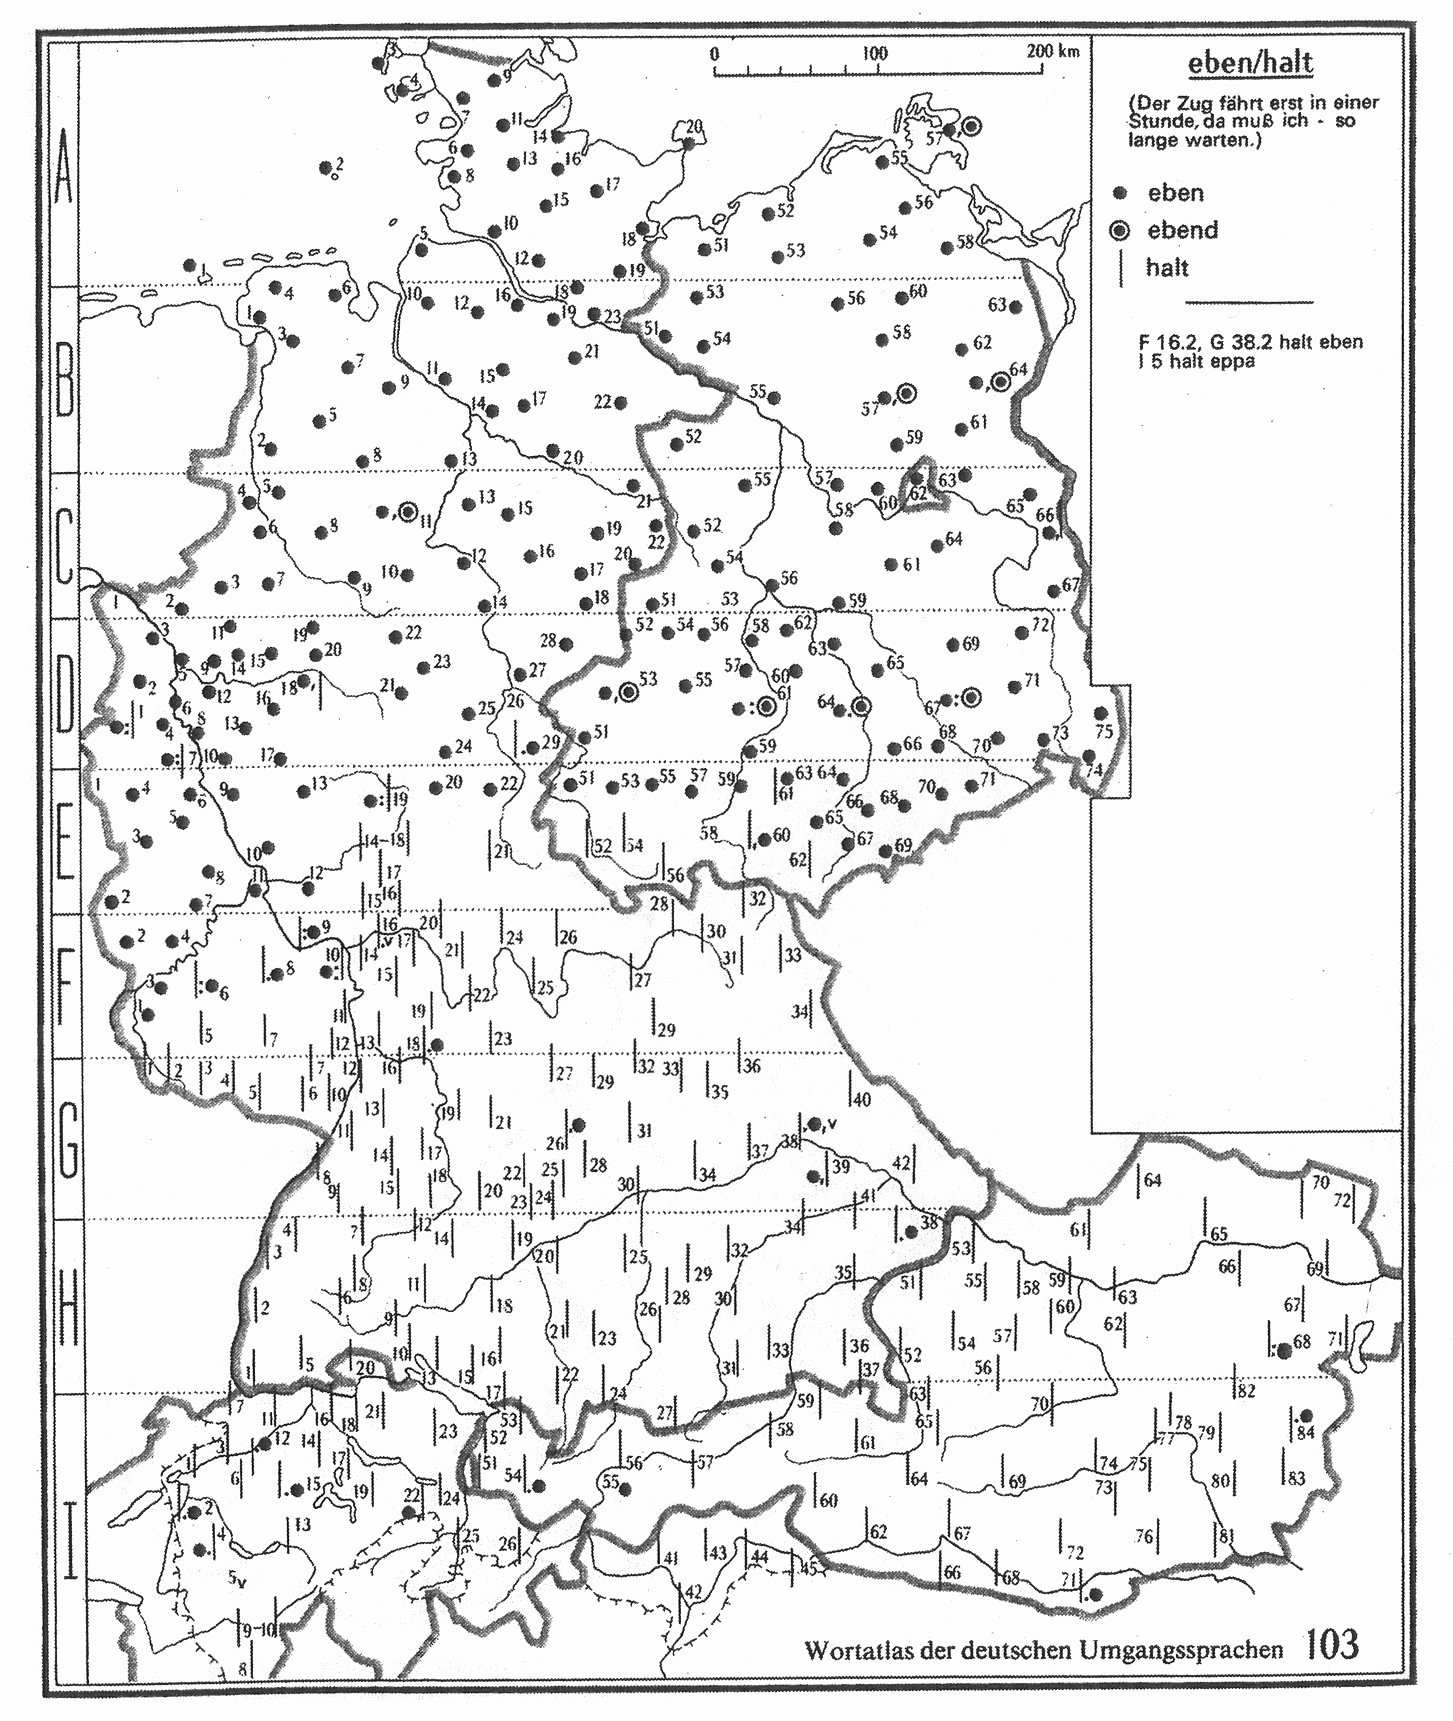
\includegraphics[width=0.7\textwidth]{he1.png}
\caption{Abbildung 1}
\label{Abbildung 1}
\hbox{}\hfill\hbox{\citet[103]{Eichhoff1978}}
\end{figure}	
\noindent
Man sieht hier eine relativ klare Trennung mit \textit{eben} in der oberen Landeshälfte und \textit{halt} in der unteren. Die Grenze verläuft nördlich der Main-Linie. Wenn andere Autoren diese Ergebnisse zusammenfassen, heißt es für die Verteilung in Deutschland, dass \textit{eben} im Norden und \textit{halt} im Süden des Landes auftritt (vgl. z.B. \citealt[212]{Dittmar2000}). Allerdings sieht man an \ref{Abbildung 1} auch, dass \textit{eben} im Süden durchaus vertreten ist, während \textit{halt} nicht im Norden auftritt.

Im Hinblick auf meine eigenen Datenerhebungen, die ich in Abschnitt~\ref{sec:spu} vorstellen werde, ist zu bedenken, dass Eichhoffs Erhebung in den 70er Jahren durchgeführt wurde (1971–1978). D.h. die damaligen Testanten sind heutzutage mindestens 60 Jahre alt (vgl. auch \citealt[2]{Elspass2005}, der hier 2005 von der Eltern- und Großelterngeneration seiner Studenten ausgeht). 

\citet{Elspass2005} berichtet von einer Nacherhebung im Stile von \citet{Eichhoff1978} in Form einer Onlinebefragung, die 2002 stattgefunden hat. Diese Untersuchung ergab die Karte in \ref{Abbildung 2}.

\begin{figure}[h]
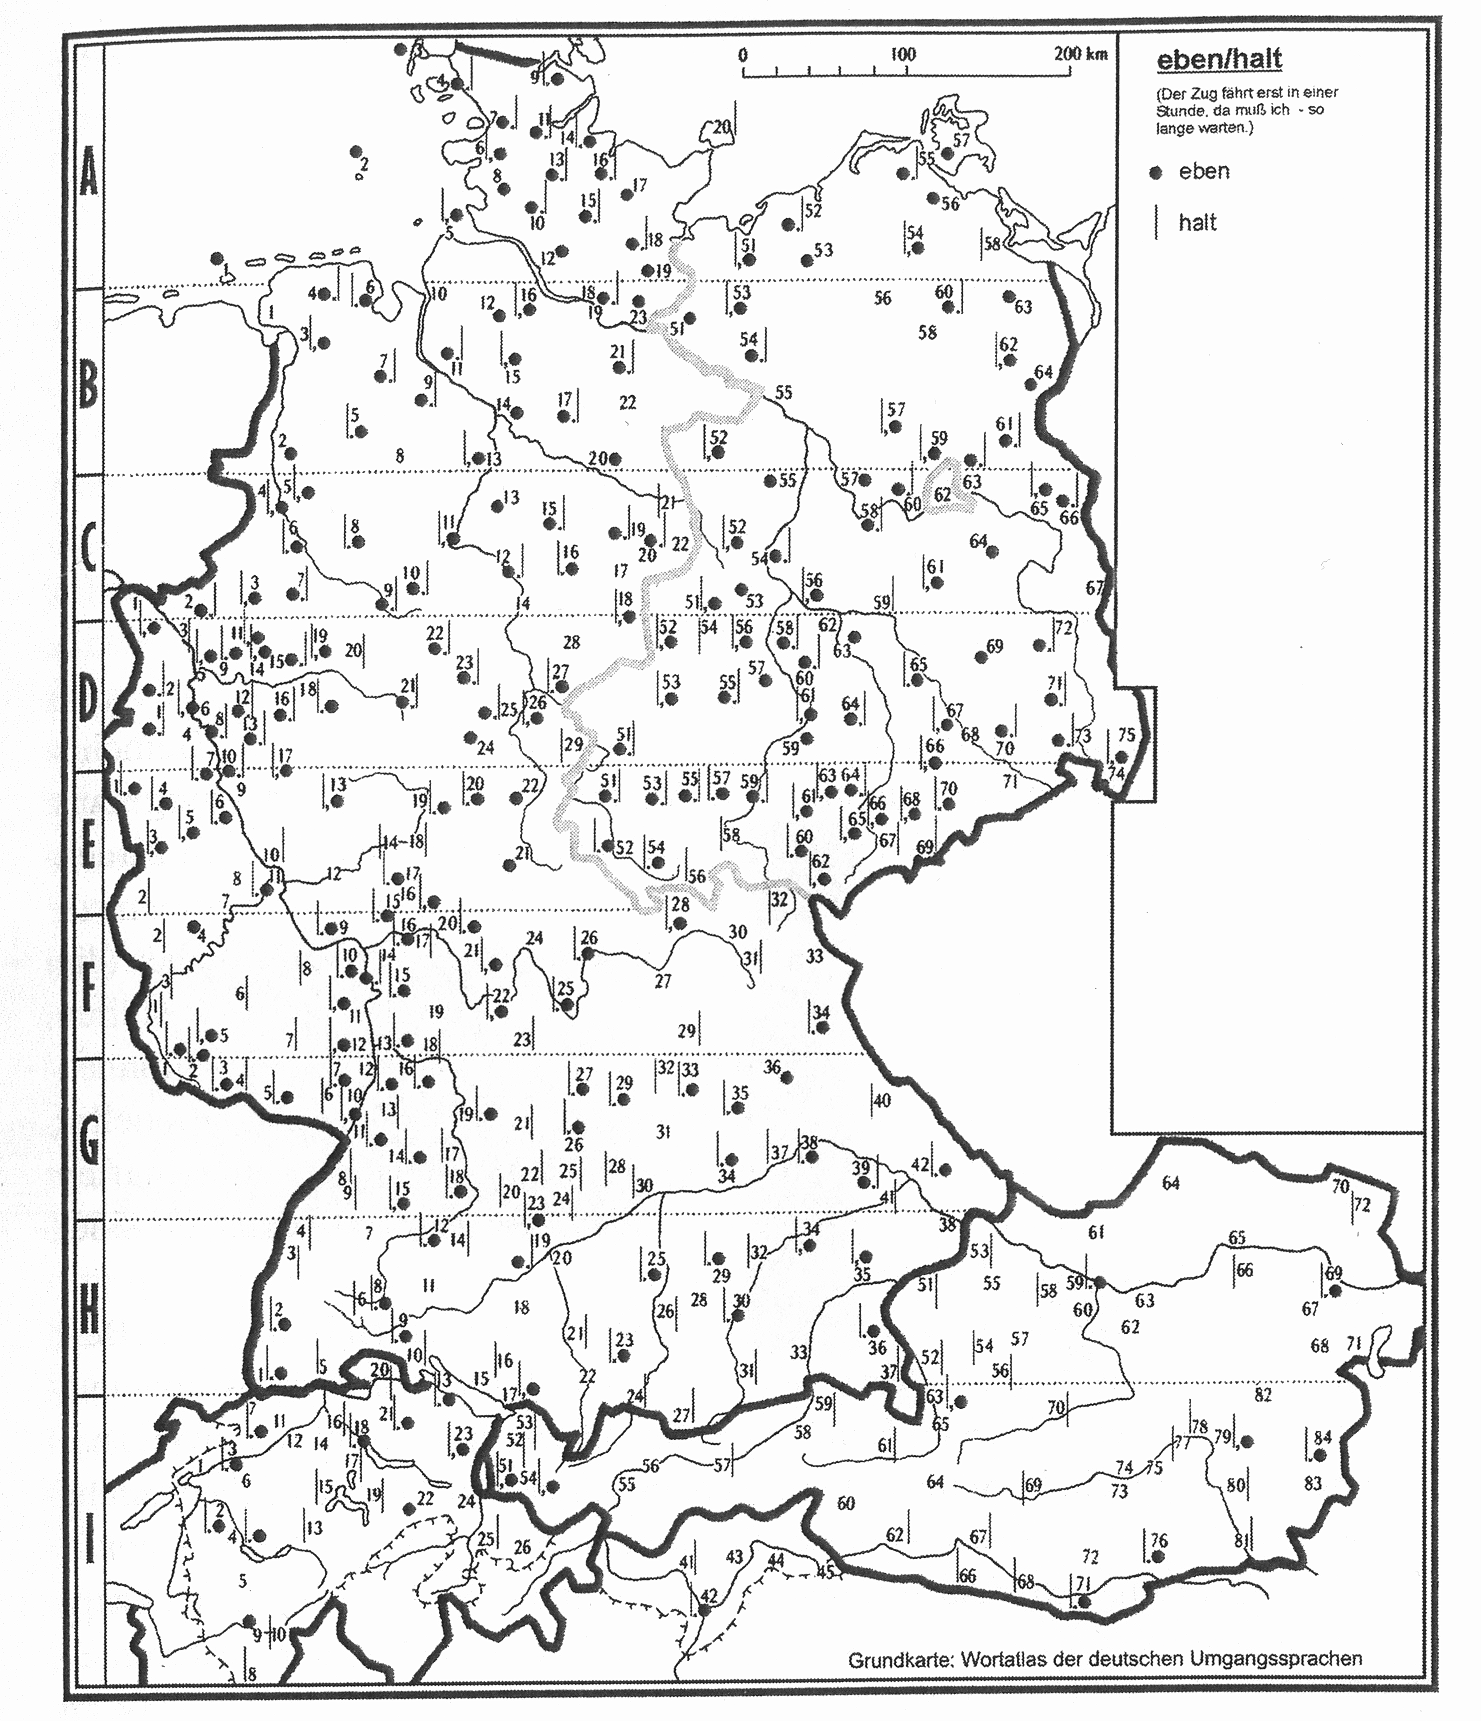
\includegraphics[width=0.7\textwidth]{he2.png}
\caption{Abbildung 2}
\label{Abbildung 2}
\hbox{}\hfill\hbox{\citet[51]{Elspass2005}}
\end{figure}
\noindent
Sie zeigt, dass sich die \textit{halt}-Verwendung in den Norden ausgeweitet hat, sowie dass \textit{eben} (wenn auch weniger) auch in anderen Gebieten auftritt.

Aus diesen Untersuchungen hat man abgeleitet, dass man es bei der Verwendung von \textit{halt} und \textit{eben} mit einem Nord-Süd-Gefälle zu tun hatte, das sich aber abgebaut zu haben scheint. Im Süden Deutschlands (bzw. in der Schweiz und Österreich) existieren \textit{halt} und \textit{eben} bereits zur Zeit der ersten Untersuchungen nebeneinander (wenngleich \textit{halt} nach \ref{Abbildung 1} zu überwiegen scheint $[$s.u. weiteres dazu$]$). Im Norden gab es Zeiten, in denen nur \textit{eben} gebräuchlich war; \textit{halt} hat aber Eingang in den Sprachgebrauch dort gefunden. Für das Gegenwartsdeutsche ist somit davon auszugehen, dass die beiden MPn im gesamten Sprachgebiet nebeneinander existieren. Dies schreiben sogar auch schon Autoren, die in den 80er Jahren auf die erste Untersuchung von Eichhoff blicken (z.B. \citealt[78]{Hartog1982}, \citealt[97]{Dahl1988}, \citealt[124]{Thurmair1989}; vgl. auch \citealt[93]{Autenrieth2002}). Die Etablierung des \textit{halt}-Gebrauchs in der oberen Landeshälfte scheint also in den 80er Jahren eingetreten zu sein.

Ähnliche Verteilungsunterschiede wurden auch für die West-Ost-Achse ange\-nommen. \citet{Protze1997} berichtet von einer Untersuchung aus der zweiten Hälfte der 70er Jahre bis 1980. Es handelt sich um Umfragen wie bei \citet{Eichhoff1977}; (\citeyear{Eichhoff1978}) die in 296 Städten der ehemaligen DDR durchgeführt wurden. Die \textit{eben}/\textit{halt}-Verteilungen, die sich auf der Basis des Testsatzes in (\ref{539}) ergaben, sind in der Karte in \ref{Abbildung 3} dargestellt.

\begin{figure}[h]
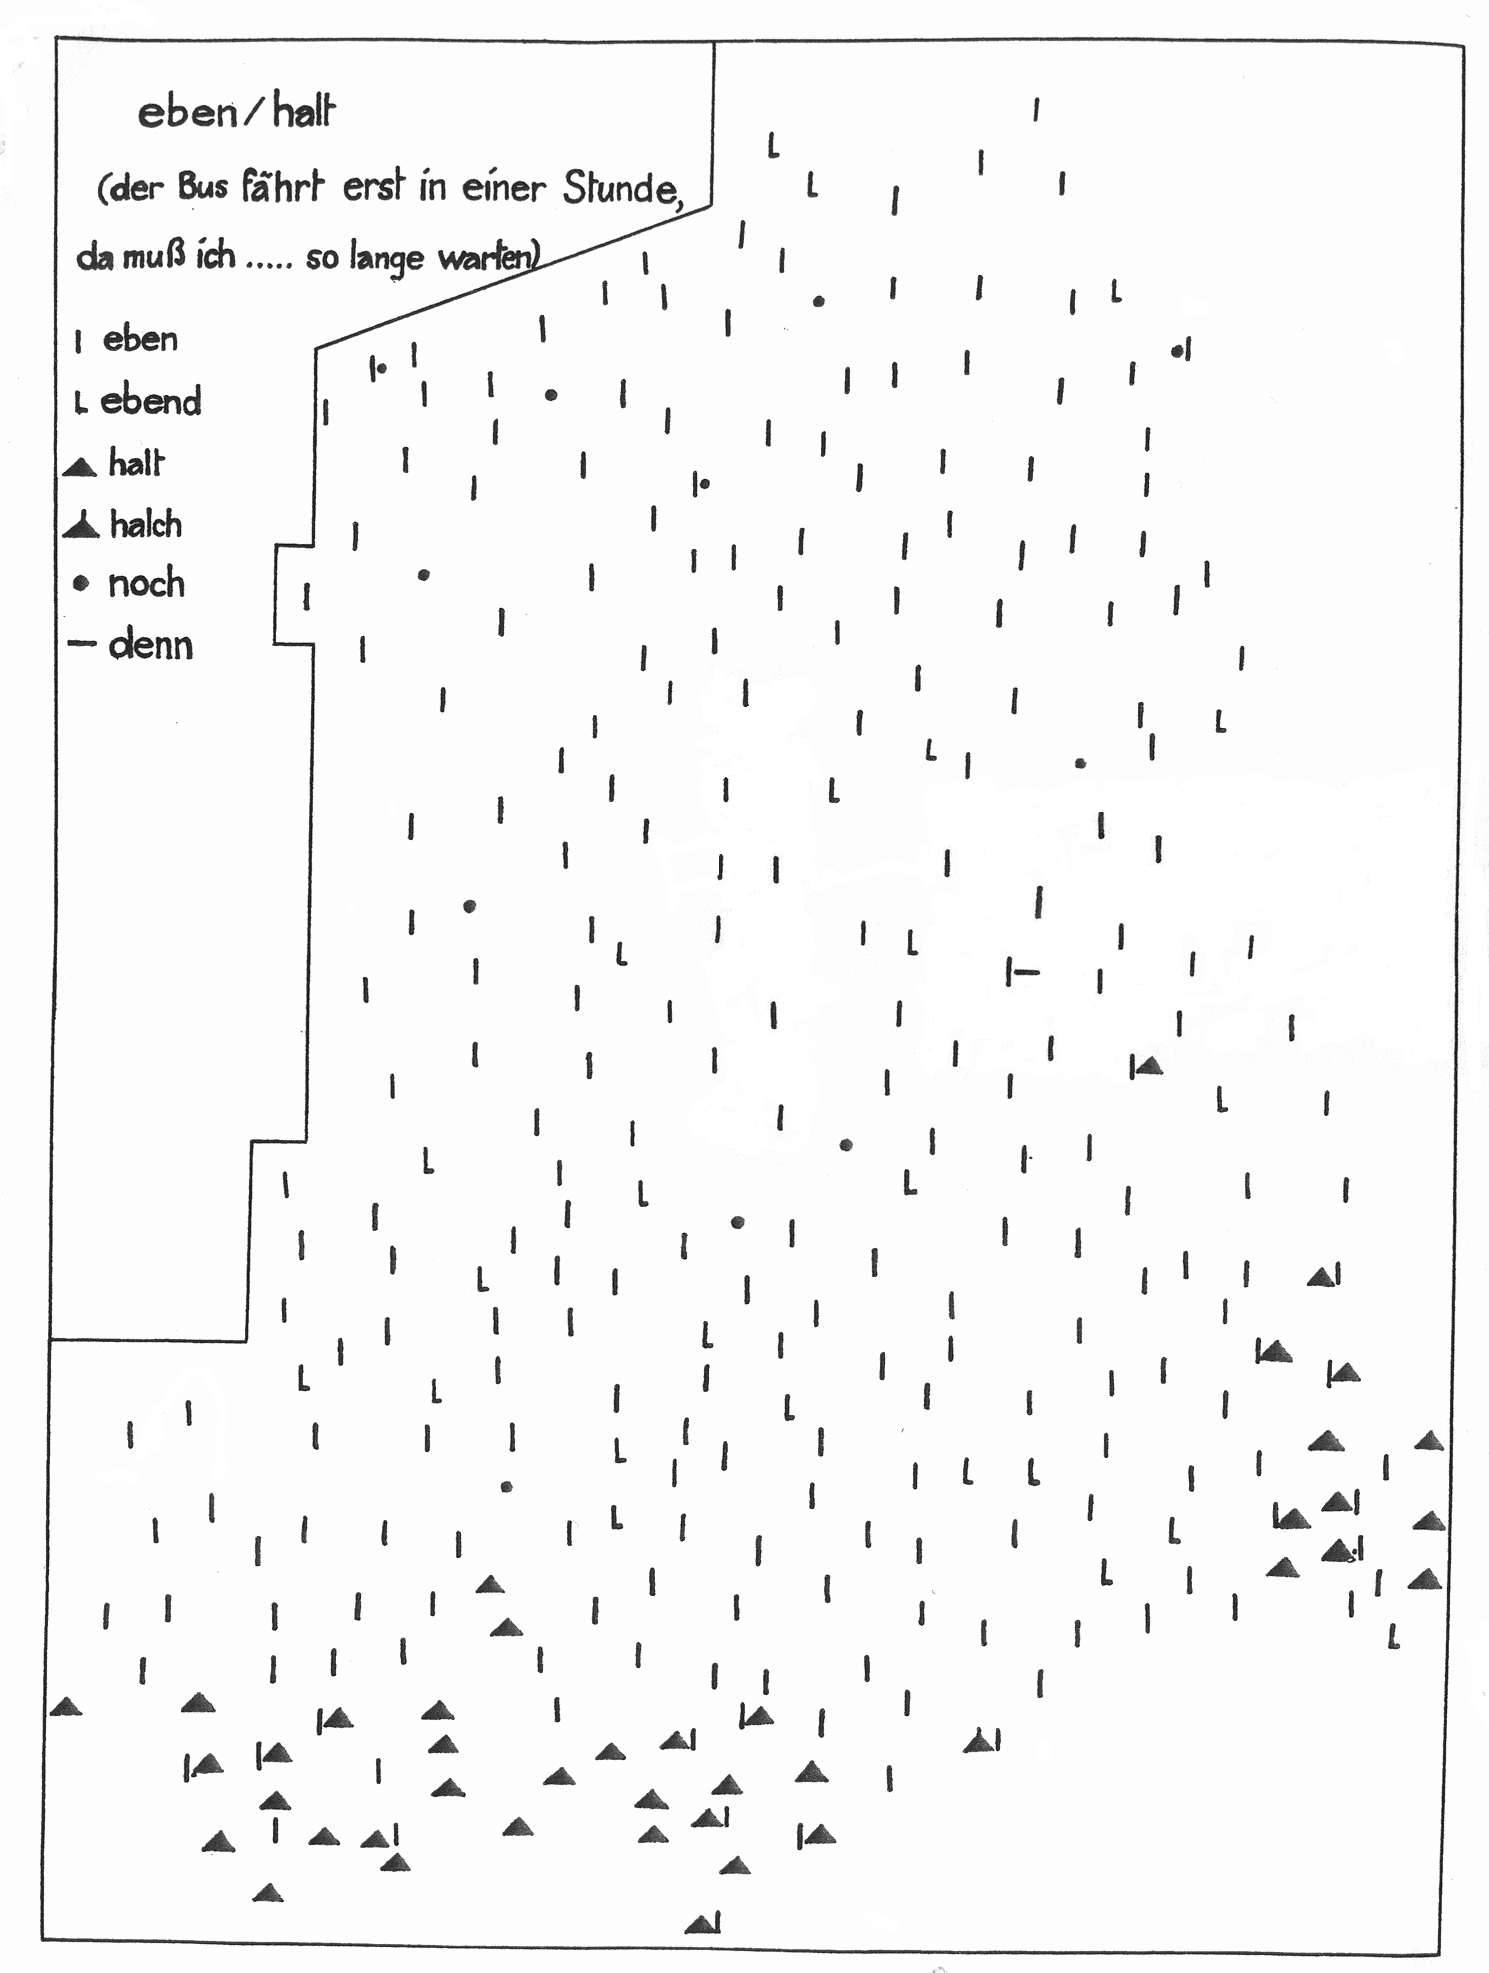
\includegraphics[width=0.5\textwidth]{he3.png}
\caption{Abbildung 3}
\label{Abbildung 3}
\hbox{}\hfill\hbox{\citet[266]{Protze1997}}
\end{figure}

\begin{exe}
	\ex\label{539} 
    Der Bus fährt erst in einer Stunde; da muß ich ... so lange warten. 
    \newline		
	\hbox{}\hfill\hbox{\citet[167]{Protze1997}}    
\end{exe}
Man sieht, dass in den neuen Bundesländern fast flächendeckend \textit{eben} verwendet wurde. Ausnahmen sind Südthüringen, das Vogtland (Südsachsen) und die Oberlausitz (Nord-Ost-Sachsen), wo \textit{halt} als gebräuchlichste Form genannt wurde.

Eine spätere Untersuchung zur unterschiedlichen Verteilung von \textit{halt} und \textit{eben} in Ost- und Westdeutschland findet sich in \citet{Dittmar2000}. Er beschäftigt sich mit den Auswirkungen von Mauerfall und Wiedervereinigung auf den Sprachgebrauch in den neuen Bundesländern. Die Datenbasis sind Interviews in Ost- und Westberlin zwischen 1993 und 1996, in denen die Befragten von ihren persönlichen Erfahrungen mit dem 09.11.1989, der Zeit danach sowie den Auswirkungen der Ereignisse auf ihre aktuelle Situation berichten. Der zentraler Punkt in \citet[213]{Dittmar2000} ist, dass die Verwendung von \textit{halt} vs. \textit{eben} einen soziolinguistischen Grund hat, in dem Sinne, dass \textit{halt} als sozialprestigeträchtig angesehen worden sei. Prinzipiell hätten die Westberliner in den Interviews häufiger \textit{halt} verwendet als die Ostberliner (s.u.). Dazu habe die \textit{halt}-Verwendung nach der \glq Wende \grq {} in Ost-Berlin und den neuen Bundesländern zugenommen. Evidenz für den hohen sozialen Status des \textit{halt}-Gebrauchs und die (daraus resultierende) Anpassung der östlichen an die westliche Sprachgemeinschaft geben metalinguistische Äußerungen wie die folgenden aus \citet[230]{Dittmar2000}.
\begin{exe}
	\ex\label{540} 
		\begin{tabular}[t]{ll} 
 		B & jo also mir' ich zucke auch zusammen eh wenn mit das \textbf{halt} raus-   \tabularnewline
 		 & rutscht;   \tabularnewline
 		I & warum? \tabularnewline
 		B & eh weil ich natürlich ganz genau weiß dieses \textbf{halt} is son marker, den' \tabularnewline
 		& den man eh bewusst setzen kann dass man \textbf{eben} sich integriert oder \tabularnewline
 		& oder dass es \textbf{eben} einfach dass es übernommen wird. \tabularnewline
 		I & wohin? \tabularnewline
 		B &	na in ein' in eine sprachgemeinschaft west;	
  		\end{tabular}				
\end{exe}																	
Dittmar gibt Häufigkeiten für jeden Sprecher zum Gebrauch von \textit{halt} und \textit{eben} in diesen Interviews an. In der Tabelle in (\ref{541}) lässt sich ablesen, dass sowohl die West- als auch die Ostberliner insgesamt häufiger \textit{eben} als \textit{halt} verwenden und dass dieses Gefälle bei den Ostberlinern außerdem stärker ausgeprägt war als bei den Westberlinern.

\begin{exe}
	\ex\label{541} 
		\begin{tabular}[t]{|l|l|l:cx{1pt}l|} 
		\hline
 		& \textit{\textbf{eben}} & \textit{\textbf{ebent}} & \textit{\textbf{eben}} & \textit{\textbf{halt}}   \tabularnewline
 		\hline
 		& & & (\textbf{gesamt}) & \tabularnewline
 		\hline
 		\textbf{31 Ostberliner} & 245 & 372 & 617 & 204 \tabularnewline
 		\hline
 		\textbf{25 Westberliner} & 213 & 96 & 309 & 161 \tabularnewline
 		\hline
  		\end{tabular}			
\end{exe}	
 		\hfill\hbox {\citet[221]{Dittmar2000}}\\
Dieser Eindruck bestätigt sich auch, wenn man die Verwendung bei den einzelnen Sprechern betrachtet. Von den 31 Ostberlinern verwenden 17, also mehr als die Hälfte, \textit{halt} gar nicht. Es gibt nur fünf Sprecher, die häufiger \textit{halt} als \textit{eben} gebrauchen, und lediglich drei, die sowohl \textit{eben} als auch \textit{halt} etwa gleich häufig verwenden. Unter den 25 Westberlinern befinden sich acht Sprecher (ca. ein Drittel), die \textit{halt} gar nicht äußern, fünf verwenden \textit{halt} häufiger als \textit{eben} und bei sechs weiteren Sprechern finden \textit{halt} und \textit{eben} etwa gleich häufig Verwendung (vgl. die Daten in \citealt[121-122]{Dittmar2000}).

Fasst man die Ergebnisse der hier skizzierten Untersuchungen zusammen, lässt sich – bis in die 70er Jahre rückblickend – sagen, dass \textit{halt} und \textit{eben} einmal regional verteilt waren: Das Süddeutsche kennt seit dieser Zeit sowohl \textit{halt} als auch \textit{eben}, das Nord- und Ostdeutsche verwendete \textit{eben} (mit einigen \textit{halt}-Flecken in Ostdeutschland). Dazu ist eine Bewegung von \textit{halt} von Süden nach Norden und von Westen nach Osten zu verzeichnen. Für das heutige Deutsch ist davon auszugehen, dass im gesamten deutschen Sprachgebiet \textit{halt} und \textit{eben} nebeneinander existieren.

\subsection{Zur Validität der dialektalen Erhebungen}
\label{sec:val}
Bei den hier skizzierten dialektalen Annahmen zu \textit{halt} und \textit{eben} handelt es sich um Aspekte, die sich bei dieser Thematik etabliert haben und die deshalb immer wieder in Arbeiten angeführt werden. Gerade deshalb halte ich es für wichtig, auch auf einige Kritikpunkte und fragliche Basen von Aussagen hinzuweisen, die z.T. auch bereits in anderen Arbeiten angeführt worden sind. Sie betreffen die Art der Fragestellung, die Auswertung und Darstellung der Ergebnisse, die Auswahl der Testsätze sowie die Repräsentativität der Ergebnisse.

Beispielsweise kritisiert \citet[16-17]{Elspass2005} mit \citet[174-178]{Hentschel1986} die Fragestellung von \citet{Eichhoff1978}, der danach fragte, ob \textit{halt}, \textit{eben} oder ein anderer Ausdruck in (\ref{542a}) verwendet werde.

\begin{exe}
	\ex\label{542a} 
 Der Zug fährt erst in einer Stunde, da muß ich .......... so lange warten.
\end{exe}																
Da es im Süddeutschen auch dialektale Formen gibt (wie \textit{ebe}, \textit{eaba}), ist es \citet[174]{Hentschel1986} zufolge unplausibel, dass der Gebrauch von \textit{halt} derart überwiegen soll. Sie nimmt an, dass \textit{halt} im Süden als mundartlicher gilt. Da die Testanten wussten, dass es sich um eine dialektale Erhebung handelt und dass \textit{halt} im Norddeutschen bzw. generell im Standarddeutschen unüblich ist, hätten sie sich (da sie sich für eine Form entscheiden mussten) für \textit{halt} entschieden, obwohl sie \textit{eben} gleichermaßen kannten. Unter dieser Sicht wären also die Art der Abfrage und die Umstände, unter denen sie stattfand, mit dafür verantwortlich, dass \textit{eben} auf der Karte in \ref{Abbildung 2} im süddeutschen Raum unterrepräsentiert zu sein scheint. Neben dem Bewusstsein um den dialektalen Status von \textit{halt}, führt \citet[176]{Hentschel1986} ebenfalls die Möglichkeit an, dass die Befragten sich für \textit{halt} entschieden, weil es positivere Konnotationen (wie \textit{weich}, \textit{warm}) aufweise. Um derartige mögliche Störfaktoren zu umgehen, beabsichtigte \citet{Elspass2005} eine Fragestellung, die die Testanten nicht zur Auswahl einer der beiden Formen zwang. Seine Formulierung lautete deshalb: \glqq Setzt man \textit{halt} oder \textit{eben}, beides oder einen anderen Ausdruck ...?\grqq{}  (\citealt[17, Fn 41]{Elspass2005} 17). Doch wie er selbst bemerkt, ist diese Version nicht eindeutig, da er mit \textit{beides} nicht auf die Nennung der Kombination der beiden MPn abzielen wollte (d.h. \textit{halt eben} oder \textit{eben halt}), sondern auf die Gleichwertigkeit der beiden Formen. Auch diese Formulierung ist nicht vollständig geglückt.

Wie die Art der Befragung bzw. die anschließende Aufarbeitung in Form der Karten Ergebnisse beeinflussen kann, zeigt auch die neueste Untersuchung zur Thematik von Elspaß \& Möller (2012) (unter http://www.atlas-alltagssprache.de/\\runde-9/). Betrachtet man die Karte in Abbildung \ref{Abbildung 4}, gewinnt man den Eindruck, \textit{eben} werde in Süddeutschland, Österreich und der Schweiz überhaupt nicht verwendet.
\begin{figure}[h]
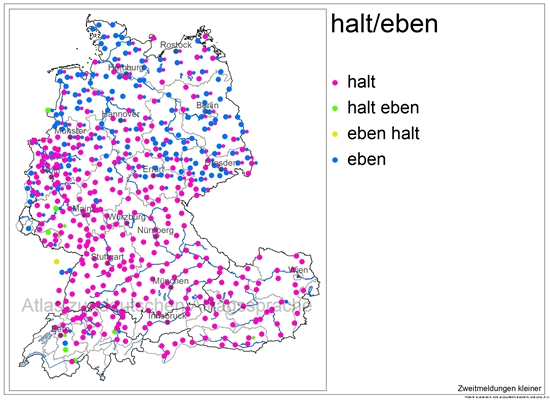
\includegraphics[width=0.7\textwidth]{he4.png}
\caption{Abbildung 4}
\label{Abbildung 4}
\hbox{}\hfill\hbox{(http://www.atlas-alltagssprache.de/halt-eben/)}
\hbox{}\hfill\hbox{(eingesehen am 05.05.2014)}
\end{figure}
\noindent																                       										
Dies verwundert, zumal dies in keiner Weise den Ergebnissen/Darstellungen der älteren Untersuchungen (weder \citealt{Eichhoff1978} noch \citealt{Elspass2005}) entspricht. Die Lösung dieses überraschenden Ergebnisses präsentieren die Autoren selbst:			
\begin{quotation}														                       										Zur Kartierung: Bei verschiedenen Antworten aus ein und demselben Ort ist die häufiger genannte Variante kartiert, in vielen Karten daneben auch (kleiner) die seltener genannte Variante, sofern sie mehr als 35\% der Nennungen ausmacht. Bei gleich häufiger Nennung musste nach dem Zufalls\-prinzip entschieden werden, welche Variante als Erst- bzw. Zweitvariante kartiert wurde. In Karten, bei denen die Wiedergabe der Zweitvarianten vor allem zur Verunklarung der regionalen Unterschiede geführt hätte, wurde der Übersichtlichkeit zuliebe darauf verzichtet. Insofern erscheinen die Unterschiede hier – gegenüber dem tatsächlichen \glqq durchschnittlichen\grqq{} Gebrauch – etwas stärker betont; dies ergibt sich aber auch schon allein aus der Art der Befragung.
\hfill\hbox{(eingesehen am 05.05.2014)}
\newline
\hbox{}\hfill\hbox{(http://www.atlas-alltagssprache.de/halt-eben)}
\end{quotation}
Wieder ist also deutlich zu sehen, dass das Ergebnis (diesmal vornehmlich durch die Art der Auswertung) verzerrt, und zwar in diesem Fall überzeichnet, wird.

Einen weiteren Aspekt gilt es in der Darstellung aus \citet{Dittmar2000} zu berücksichtigen. Er weist selbst darauf hin, dass seine Ergebnisse nur bedingt aussagekräftig sind, da einerseits die Informantenzahl verschieden (25 West- vs. 31 Ostberliner) und andererseits die Interviewausschnitte unterschiedlich lang waren (vgl. \citealt[222]{Dittmar2000}). Vor diesem Kritikpunkt ist Dittmars Ergebnis, dass mehr Westberliner \textit{halt} überhaupt benutzen, allerdings auch umso bedeutender, da die Interviews mit den Ostberlinern sogar länger sind und sie somit mehr Möglichkeiten hatten, \textit{halt} zu verwenden (wenn sie es überhaupt verwenden) (vgl. \citealt[222]{Dittmar2000}).

Ein letzter Aspekt, der in den Untersuchungen von Eichhoff, Elspaß und Protze nicht genügend Beachtung findet, ist die Frage, ob in dem einen (!) vorgegebenen Testitem tatsächlich \textit{halt} und \textit{eben} gleichermaßen verwendet werden können. Ich möchte meine konkreten Bedenken auf Abschnitt~\ref{sec:spu} verschieben, um unter Bezug auf meine Bedeutungsmodellierung präziser argumentieren zu können. An dieser Stelle sei aber bereits angemerkt, dass der regionale Charakter (insbesondere bei prinzipieller Bekanntheit beider Formen) wohl nur nachweisbar ist, wenn die beiden MPn in der vorliegenden Äußerung tatsächlich beide gleichermaßen plausibel auftreten können. Im Rahmen ihrer Analyse der Interpretation von \textit{halt} und \textit{eben} bezweifelt auch schon \citet[174]{Hentschel1986} dies in Bezug auf Eichhoffs Testsatz. Nach der Autorin ist \textit{halt} emotionaler konnotiert als \textit{eben} und der Kontext in (\ref{542a}) lege diese Lesart nahe.

\subsection{Die Bedeutung von \textit{halt} und \textit{eben}}
\label{sec:bedhe}
Wenn Autoren annehmen, dass es die zwei Formen \textit{halt} und \textit{eben} deshalb gibt, weil sie regional verteilt sind, geht diese Sicht damit einher, dass sie ihre Bedeutung und Verwendung für identisch halten (vgl. z.B. \citealt[10]{Becker1978}, \citealt[358]{Luetten1977}, \citealt[81]{Bublitz1978}, \citealt[202]{Karagjosova2004}). Es wird dann eine Bedeutung für \textit{eben} angegeben, die auf \textit{halt} gleichermaßen zutreffen soll. Wenige Autoren beschäftigen sich hingegen mit der Bedeutung von \textit{halt} und betrachten es in Differenz zu \textit{eben}. Die Bedeutung, die von ersteren Autoren sowohl für \textit{halt} als auch für \textit{eben} angesetzt wird, ist dann in der Regel diejenige, die Autoren, die sich für einen Unterschied zwischen den beiden Partikeln aussprechen, für \textit{eben} formulieren.

\subsubsection{Gemeinsamkeiten}
Die Illokutionstypen, in denen \textit{halt} und \textit{eben} auftreten können, sind Assertionen \is{Assertion} und \is{Direktiv} Direktive.\footnote{Die beiden Partikeln können auch in verschiedenen Nebensatztypen auftreten, vor allem \textit{halt} scheint hier
sehr frei verwendet werden zu können (z.B. Kausalsätze, Konditionalsätze, Temporalsätze, Instrumentalsätze $[$zu einem Überblick vgl. \citealt[202-203]{Hentschel1986}$]$). Ich gehe auf die Nebensatzverwendungen an dieser Stelle nicht ein, betrachte in Abschnitt~\ref{sec:rs} allerdings ihr Auftreten in Relativsätzen sehr detailliert.}

\begin{exe}
	\ex\label{542} Assertion\\
	A: Peter sieht sehr schlecht aus. (= q)\\
	B: Er war \textbf{eben}/\textbf{halt} lange krank gewesen. (= p)		
\end{exe}	

\begin{exe}
	\ex\label{543} Direktiv\\
	A: Ich schaffe es nicht bis morgen! (= q)\\
	B: Arbeite eben/halt schneller! (= p)	
	\hfill\hbox{\citet[340/215]{Karagjosova2004}} 	
\end{exe}				    
Die klassischen Merkmale, die in Beschreibungen dieser zwei Partikeln genannt werden (vgl. auch \citealt[150-152]{Mueller2016a}; \citeyear[165-169]{Mueller2016b}, \citeyear[239-243]{Mueller2017a}), sind zum einen die \textit{Rückorientierung} von \textit{eben}/\textit{halt}-Äußerungen und zum anderen der Aspekt der \textit{Kategorizität}. Die Eigenschaft der Rückorientierung (vgl. z.B. \citealt[98, 224]{Dahl1988}, \citealt[120, 125-126]{Thurmair1989}, \citealt[340]{Karagjosova2003}; \citeyear[208]{Karagjosova2004}) zeigt sich generell darin, dass diese MP-Äußerungen immer Reaktionen auf eine vorausgehende Äußerung oder Situation sind. Wie in Abschnitt~\ref{sec:zugang} in Kapitel~\ref{chapter:hintergrund} erläutert, sind MPn prinzipiell reaktiver Natur. Diese Eigenschaft trifft auf \textit{halt} und \textit{eben} aber umso mehr zu, da die Bedingung bzw. das Begründende vorerwähnt sein muss. Sie können nicht redeeinleitend verwendet werden und eignen sich nicht zum Themenwechsel. Konkreter wird für diese Relation angenommen, dass die MP-Äußerung und eine andere Äußerung in einem kausalen Verhältnis \is{kausale Relation} zueinander stehen oder eine Bedingungs-Folge-Relation \is{Bedingungs-Folge-Relation} vorliegt (vgl. z.B. \citealt[40]{Weydt1969}, \citealt[101, 288 Fn 60, 125]{Dahl1988}, \citealt[121]{Helbig1990}, \citealt[67]{Koenig1997}). 

In (\ref{542}) beispielsweise ist das Kranksein die Begründung für das schlechte Aussehen. Die MP-Äußerung gibt hier den Grund für den Inhalt der vorausgehenden Äußerung an (vgl. (\ref{544})).

\begin{exe}
	\ex\label{544} Weil er lange krank gewesen ist (= p), sieht Peter schlecht aus (= q).		
\end{exe}
Mit dieser Funktion der \textit{eben}/\textit{halt}-Äußerung ist gut verträglich, dass einer solchen Äußerung gerne eine Frage nach dem Grund vorweggeht (vgl. (\ref{545}), (\ref{546}) (vgl. \citealt[121]{Thurmair1989})).
\begin{exe}
	\ex\label{545} 
	Hans: Warum sind nur die Frauen so hinter dir her?\\
	Peter: Ich bin \textbf{eben} unwiderstehlich.
	\hfill\hbox{\citet[121]{Thurmair1989}} 	
\end{exe}	

\begin{exe}
	\ex\label{546} 
	Warum bist du denn so fad?\\
	Ich bin \textbf{halt} krank.	
	\hfill\hbox{\citet[312]{Schlieben-Lange1979}} 	
\end{exe}	
Eine Äußerung ohne Partikel ist hier situativ unangemessen und das Auftreten einer kausalen Konjunktion ist in diesem Fall notwendig (vgl. (\ref{547})).

\begin{exe}
	\ex\label{547} 
	Hans: Warum sind nur die Frauen so hinter dir her?\\
	Peter: ?Ich bin unwiderstehlich./Weil ich unwiderstehlich bin.	
	\newline
	\hbox{}\hfill\hbox{\citet[121]{Thurmair1989}} 	
\end{exe}
Bei den \glq Begründungen\grq {} muss es sich dabei nicht um tatsächliche Begründungen handeln. In (\ref{548}) und (\ref{549}) liegen keine oder nur sehr oberflächliche Begründungen vor (vgl. \citealt[322]{Troemel-Ploetz1979}).

\begin{exe}
	\ex\label{548} 
	Wieso muss man denn hier fünf Fragebögen ausfüllen? – Das ist \textbf{eben} so.	
	\newline
	\hbox{}\hfill\hbox{\citet[312]{Schlieben-Lange1979}} 	
\end{exe}	
\begin{exe}
	\ex\label{549} 
	Warum esst ihr denn mit Stäbchen? – Das gefällt uns \textbf{eben}.
	\newline
	\hbox{}\hfill\hbox{\citet[322]{Troemel-Ploetz1979}} 	
\end{exe}																	              
Ein Beispiel für eine Bedingungs-Folge-Relation findet sich in (\ref{550}).

\begin{exe}
	\ex\label{550} 
	Evi: Du, das ist ganz blöd heute, ich hab noch so wahnsinnig viel zu tun. 
	\newline
	\hbox{}\hfill\hbox{(= q)}\\
	Pit: Gut, komm ich \textbf{halt}/\textbf{eben} morgen. (= p) So dringend ist es ja nicht.
	\newline
	\hbox{}\hfill\hbox{nach \citet[122]{Thurmair1989}} 	
\end{exe}

\begin{exe}
	\ex\label{551} 
	\glq Wenn du so viel zu tun hast (= q), dann komme ich morgen (= p).\grq {} 	
\end{exe}
Assertive Fälle können sowohl den Grund (vgl. (\ref{542})) als auch (wie in (\ref{550})) die Folge angeben. In Direktiven scheint mir der MP-Teilsatz immer die Folge auszumachen (vgl. (\ref{543}) und (\ref{552})).

\begin{exe}
	\ex\label{552} 
	Wenn du es nicht bis morgen schaffst (= q), musst du schneller arbeiten. 
	\newline
	\hbox{}\hfill\hbox{(= p)} 	
\end{exe}
Ein anderes Merkmal, das bei der Charakterisierung von \textit{eben} (und ggf. auch \textit{halt}) angeführt wird, ist das der \textit{Kategorizität}. 

Bei \citet[120-121]{Helbig1990} und \citet[340]{Karagjosova2003} heißt es über \textit{halt} und \textit{eben}, der Sachverhalt werde als \textit{unabänderlich}, \textit{kategorisch} und \textit{Thema beendend} ausgegeben. \citet[80/83]{Autenrieth2002} spricht von \textit{Absolutheit} und \textit{Kategorizität}. \citet[120]{Thurmair1989} schreibt, der Sachverhalt sei \textit{evident} (zu \textit{eben}). In Direktiven entspricht dies dem Verhältnis, dass die Handlung, zu der aufgefordert wird, \textit{offensichtlich} ist und die \textit{einzig mögliche Lösung des Problems} darstellt (vgl. \citealt[122]{Thurmair1989}, vgl. auch \citealt[169]{Hentschel1986}). Wie für alle mit MPn erreichten Effekte gilt auch hier, dass die Bedeutungsmomente \textit{Evidenz} und \textit{Faktum} auch nur vorgegeben sein können. \citet[320-323]{Troemel-Ploetz1979} nimmt für \textit{eben} an, die MP gebe die Proposition als \textit{generell gültig} und als \textit{Faktum} aus. Der Hörer könne die Annahme nicht in Frage stellen oder ihr widersprechen. Weitere Diskussionen würden sich erübrigen. Die Aussage werde als \textit{axiomatisch} dargestellt und die Behauptung somit \textit{immunisiert}. Auch die Auffassung von \citet[130]{Diewald1997} zu \textit{eben}, die Proposition sei \glqq bereits gegeben und aktuell wiederholt\grqq{} fügt sich in dieses Bild ein. \citet{Autenrieth2002} weist anhand von Beispielen der Art in (\ref{553}) darauf hin, dass die Charakterisierung \textit{unabänderlich} ggf. auch zu stark ausfalle, da auf solche Äußerungen eher verwandte, aber schwächere Bedeutungs\-zuschreibungen wie \textit{unspektakulär}, \textit{unproblematisch} und \textit{gewöhnlich} zutreffen würden.

\begin{exe}
	\ex\label{553} 
	(S zeigt Foto)\\
	Und auf DIEsem Foto ist Beates Kuchen dann \textbf{halt}/\textbf{eben} fertig und steht auf dem Tisch.		
	\hfill\hbox{nach \citet[99]{Autenrieth2002}} 
\end{exe}
Es ist auch darauf hingewiesen worden, dass sich die Bedeutungseffekte \textit{Evidenz} und \textit{Kategorizität} ebenfalls auf die Relation und nicht (nur) auf die Proposition der MP-Äußerung beziehen können (vgl. \citealt[99]{Dahl1988}). In (\ref{554}) wird nach Dahls Argumentation (zu \textit{eben} und \textit{halt}) nicht der Sachverhalt, dass der Nachbar Choleriker ist, als kategorisch/axiomatisch ausgegeben, sondern die Relation zwi\-schen den Propositionen (der Nachbar macht Krach und der Nachbar ist Choleriker).

\begin{exe}
	\ex\label{554} 
	A: Unser Nachbar hat heute wieder Krach gemacht.\\
	B: Er ist \textbf{eben} ein Choleriker.		
	\hfill\hbox{nach \citet[98]{Dahl1988}} 
\end{exe}
In (\ref{555}) ist der Zusammenhang bekannt:
\begin{exe}
	\ex\label{555} 
	Wenn jemand Choleriker ist, wird es bei ihm auch manchmal laut.
\end{exe}
Dahl nimmt dazu an, die \textit{eben}-Äußerung wirke \textit{abqualifizierend} (\citeyear[100]{Dahl1988}), in dem Sinne, dass B die Berechtigung der vorausgehenden Äußerung bestreitet. B widerspricht den Erwartungen, die A mit seiner Äußerung ausdrückt. Im Falle einer Assertion wie in (\ref{554}) ist dies die Annahme, dass er B etwas mitteilt, das wissenswert ist. Diese Erwartung wird in (\ref{554}) gestört, weil die Proposition aus As Äußerung ableitbar ist. Parallele Verhältnisse liegen auch in Direktiven wie in (\ref{556}) vor.
\begin{exe}
	\ex\label{556} 
	A: Mein Zahn tut mir weh.\\
	B: Dann geh \textbf{eben} zum Zahnarzt!
	\hfill\hbox{nach \citet[101]{Dahl1988}} 
\end{exe}
A müsste hier selbst zum Schluss der \textit{eben}-Äußerung kommen, da der Zusammenhang in (\ref{557}) bekannt ist.
\begin{exe}
	\ex\label{557} 
	Wenn dein Zahn weh tut, musst du zum Zahnarzt gehen.
\end{exe}
Es besteht kein Grund zum Klagen für A und die Mitteilung von A ist für die Eröffnung eines Problemlösungsszenarios irrelevant. Auch hier bestreitet B die Berechtigung des vorweggehenden Sprechaktes.

Diese Überlegungen stammen aus \citet[98-101]{Dahl1988} und werden in \citet[340]{Karagjosova2003}; (\citeyear[202-220]{Karagjosova2004}) übernommen, um die Bedeutung von \textit{eben} und \textit{halt} in einem formalen Diskursmodell zu erfassen. Da ich auf ihre Bedeutungszuschreibung in Abschnitt~\ref{sec:modellierung} zurückgreifen werde, seien ihre Annahmen an dieser Stelle bereits angeführt.

Auf der Basis der beiden Kriterien a) Rückorientierung und b) Kategorizität fasst die Autorin den Beitrag von \textit{eben} und \textit{halt} folgendermaßen auf: Zum einen ist die Proposition der MP-Äußerung bekannt. Dies kann p oder q sein (s.u.). Zum anderen ist unter den Diskurspartnern die Inferenzrelation p $>$ q (\glq Normalerweise, wenn p, dann q.\grq {}) bekannt. p $>$ q hat in \citet{Asher1991}, auf die sich Karagjosova hier bezieht, den Status \is{defeasible rule} einer \textit{defeasible rule}. Fungiert die \textit{eben}/\textit{halt}-Äußerung als Begründung der vorweggehenden Äußerung wie in (\ref{558}), ist p bekannt sowie die Inferenzrelation p $>$ q.
\begin{exe}
	\ex\label{558} 
	A: Unser Nachbar hat heute wieder Krach gemacht. (= q)\\
	B: Er ist \textbf{eben} ein Choleriker. (= p)
\end{exe}
Über \textit{modus ponens} \is{modus ponens} unter Beteiligung dieser (pragmatischen) Inferenzrelation, an dem nor\-malerweise ein \underline{logischer} Zusammenhang zwischen p und q beteiligt ist, ist abzuleiten, dass auch q bekannt ist (\textit{deafisible modus ponens} \is{deafisible modus ponens} in \citealt[387]{Asher1991}). 

Stellt die MP-Äußerung die Folge in einem Bedingungs-Folge-Gefüge dar wie in (\ref{559}), dreht sich die Inferenzrelation um. D.h. die Relation q $>$ p ist bekannt, ebenso die Proposition p.\footnote{Alternativ bleibt die Inferenzrelation p $>$ q und die MP bezieht sich auf q (und nicht p).}

\begin{exe}
	\ex\label{559} 
	A: Ich schaffe es nicht bis morgen. (= q)\\
	B: Arbeite \textbf{eben}/\textbf{halt} schneller! (= p)
\end{exe}	
Nach As Äußerung sind A und B sich hinsichtlich q einig. (A ist von q aufgrund seiner Äußerung überzeugt, B gibt einen Rat unter den Umständen von q, was auf seine Akzeptanz von q schließen lässt.) Ebenfalls bekannt ist der Zusammenhang zwischen q und p (\glq Wenn du etwas nicht bis zum nächsten Tag schaffst, musst du schneller arbeiten.\grq {}). Wenn q und q $>$ p bekannt ist, ist auch klar, dass zu p geraten wird.

Karagjosova setzt den hier beschriebenen Effekt sowohl für \textit{halt} als auch für \textit{eben} an. Wie eingangs angeführt, gibt es allerdings auch Autoren, die in ihrer Charakterisierung einen Unterschied zwischen den beiden Partikeln machen.

\subsubsection{Unterschiede}
\label{sec:untersch}
\citet[124]{Thurmair1989} geht davon aus, dass die beiden MPn zwar eine ähnliche Bedeutung haben, es sich aber nicht um Synonyme handelt. Auch \citet[254]{Dahl1988} schreibt schon, \glqq daß es sich eher um funktionale Ähnlichkeit als Äquivalenz\grqq{}  handelt. Eines der Argumente für diese Annahme ist bei \citet{Thurmair1989}, dass \textit{eben} und \textit{halt} nicht beliebig austauschbar sind. So gibt es Kontexte, in denen \textit{eben} im Gegensatz zu \textit{halt} nicht gut stehen kann (vgl. (\ref{5600}) und (\ref{561})).\footnote{Ein Gutachter weist korrekterweise darauf hin, dass ein Beispiel wie (\ref{5600}) zeigt, dass die beteiligte Begründung nicht einer vorher explizit genannten Proposition gelten muss, sondern eine \textit{halt}-/\textit{eben}-Äußerung sich auch auf eine Implikatur der Vorgängeräußerung beziehen kann. In (\ref{5600}) werde nicht die Proposition dass der Adressat seine Freunde mitbringen kann begründet, sondern der durch \textit{schon} ausgedrückte Vorbehalt gegenüber weiteren Gästen.}

\begin{exe}
	\ex\label{5600} Du kannst deine Freunde schon mitbringen.
		\begin{xlist}	
			\ex\label{560a} Wir haben \textbf{halt} kein Bier mehr.
			\ex\label{560b} *Wir haben \textbf{eben} kein Bier mehr.
		\end{xlist}
\end{exe}

\begin{exe}
	\ex\label{560} Monika will Hans um einen Gefallen bitten, zögert aber, ihn anzurufen. Nach einiger Zeit sagt ihre Freundin.
		\begin{xlist}	
			\ex\label{560a} Jetzt ruf den Hans \textbf{halt} an!
			\ex\label{560b} *Jetzt ruf den Hans \textbf{eben} an!
			\hfill\hbox {\citet[124]{Thurmair1989}}
		\end{xlist}
\end{exe}
Umgekehrt sind ihrer Ansicht nach schwieriger Fälle zu finden, in denen \textit{eben} angemessen ist und \textit{halt} unpassend erscheint. Thurmair gibt die Beispiele in (\ref{561}) und (\ref{562}).

\begin{exe}
	\ex\label{561} 
		\begin{xlist}	
			\ex\label{561a} Der Wal ist \textbf{eben} ein Säugetier.
			\ex\label{561b} ?Der Wal ist \textbf{halt} ein Säugetier.
		\end{xlist}
\end{exe}
\begin{exe}
	\ex\label{562} 
		\begin{xlist}	
			\ex\label{562a} Der Krieg ist \textbf{eben} unmoralisch.
			\ex\label{562b} ?Der Krieg ist \textbf{halt} unmoralisch.
			\hfill\hbox {\citet[124]{Thurmair1989}}
		\end{xlist}
\end{exe}
Und auch wenn beide Partikeln in einem Kontext prinzipiell stehen können (vgl. (\ref{563}), (\ref{564})), geht das Auftreten der ein oder anderen Partikel der Autorin zufolge mit einem Interpretationsunterschied einher.

\begin{exe}
	\ex\label{563} 
		\begin{xlist}	
			\ex\label{563a} Männer sind \textbf{eben} so.
			\ex\label{563b} Männer sind \textbf{halt} so.
		\end{xlist}
\end{exe}
\begin{exe}
	\ex\label{564} Ich hab dich doch gewarnt. 
		\begin{xlist}	
			\ex\label{564a} Horrorvideos sind \textbf{eben} grausam.	
			\ex\label{564b} Horrorvideos sind \textbf{halt} grausam.
			\hfill\hbox {\citet[124]{Thurmair1989}}
		\end{xlist}
\end{exe}
Eine \textit{halt}-Äußerung wirke im Vergleich zu einer \textit{eben}-Äußerung abgeschwächter und weniger apodiktisch (vgl. \citealt[125]{Thurmair1989}, vgl. auch schon \citealt[309]{Schlieben-Lange1979}). Wie oben erläutert, zeigen \textit{halt} und \textit{eben} hinsichtlich des Kriteriums des Rückbezugs dasselbe Verhalten. Im Falle von \textit{halt} ist der Sachverhalt (bzw. die Relation) nicht evident/kategorisch/die einzige Möglichkeit, sondern nur plausibel. Die \textit{halt}-Äußerung ist eine plausible Erklärung/Begründung für den Vorgängerbeitrag oder eine plausible Folge aus diesem. Im Falle einer \textit{halt}-Begründung/Erklärung sind alternative Begründungen zugelassen. Der Sprecher vertritt lediglich die von ihm präsentierte Erklärung. Insgesamt wirken \textit{halt}-Assertionen somit abgeschwächter im Vergleich zu \textit{eben}-Assertionen. \textit{Halt}-Auffor\-derungen, \is{Aufforderung} die die Folge aus dem zuvor gesagten darstellen, sind schwächer als \textit{eben}-Aufforderungen. Sie präsentieren nicht apodiktisch die einzig denkbare Lösung, sondern es handelt sich aus Sprechersicht um eine plausible Lösung für das Problem aus dem Vorgängerbeitrag (vgl. \citealt[125-126]{Thurmair1989}, vgl. auch \citealt[316]{Schlieben-Lange1979}, \citealt[74-75]{Hartog1982}, \citealt[235]{Meibauer1994}, \citealt[312]{Rost-Roth1998}, \citealt[98]{Autenrieth2002}).

Unter der Annahme dieses Unterschieds in der Interpretation von \textit{eben}- und \textit{halt}-Äußerungen leitet \citet{Thurmair1989} die Beispiele aus (\ref{560}) und (\ref{561}), in denen die beiden MPn situativ nicht gleichermaßen angemessen sind, auf die folgende Art ab: Sie argumentiert, dass \textit{eben} dann inakzeptabel ist, wenn Alternativen relevant sind und anerkannt werden. In Beispielen der Art in (\ref{560}) und (\ref{561}) stellt der Sachverhalt der MP-Äußerung eine plausible Begründung dar, der Sprecher bzw. der Adressat handelt aber nicht danach. In (\ref{560}) ist es beispielsweise plausibel für den Sprecher, dass, wenn man kein Bier mehr hat, man nicht weitere Gäste einlädt. Dies scheint aber nicht der einzige Zusammenhang zu sein: Wenn dies der einzige denkbare Zusammenhang wäre, könnte er die Freunde schließlich nicht zulassen. Ist die MP-Äußerung die Folge wie im Falle der Aufforderung in (\ref{561}), handelt es sich bei der Handlung, zu der geraten wird, um eine plausible, aber wiederum nicht einzig mögliche Lösung. Den Gesprächspartner anzurufen, ist \underline{eine} Möglichkeit, es ist aber nicht die einzige. Aus dem Kontext ist bekannt, dass der Vorschlag gerade nicht evident ist, da der Adressat genau diese Handlung nicht favorisiert (vgl. \citealt[127]{Thurmair1989}).

In Abschnitt~\ref{sec:modellierung} werde ich erläutern, wie sich diese Fälle in meine Bedeutung\-smodellierung fügen. Die entscheidende Erkenntnis von Thurmair an dieser Stelle, die es m.E. bei jeder Modellierung des Beitrags von \textit{halt}- und \textit{eben}-Äußerungen zu berücksichtigen gilt, ist, dass sich Beispiele finden lassen, in denen \textit{halt} stehen kann, in denen das Auftreten von \textit{eben} aber hingegen nicht angemessen ist. Es handelt sich um Situationen, in denen nicht von Evidenz/Kategorizität, sondern schwächer von Plausibilität auszugehen ist. Umgekehrt ist \textit{halt} dann nicht passend, wenn der ausgedrückte Sachverhalt evident ist. Es ist in diesem Fall nicht angemessen, Alternativen offen zu halten; \textit{halt} ist in diesem Sinne dann zu schwach. Es scheint äußerst unwahrscheinlich, dass nur der Sprecher davon ausgeht, dass der Wal ein Säugetier oder Krieg unmoralisch ist (vgl. (\ref{560}) und (\ref{561})). In Äußerungen dieser Art ist somit nur \textit{eben} zu verwenden. Die Fälle, in denen das Auftreten von \textit{halt} im Gegensatz zu \textit{eben} unangemessen ist, sind allerdings sehr selten (vgl. \citealt[128]{Thurmair1989}).

Die MP \textit{eben} lässt sich folglich in der Regel durch \textit{halt} ersetzen. Der umgekehrte Austausch ist hingegen nicht immer möglich (vgl. \citealt[128]{Thurmair1989}, \citealt[392]{Ickler1994}). Wenn \textit{eben} (mit Thurmair, s.o.) Evidenz anzeigt und \textit{halt} Plausibilität, sind die obigen Verhältnisse folgendermaßen zu erklären: Ein evidenter Sachverhalt ist auch plausibel, eine plausible Sachlage ist aber nicht notwendigerweise evident. In diesem Sinne schließt die Bedeutung von \textit{eben} die Bedeutung von \textit{halt} ein, der Beitrag von \textit{halt} schließt aber nicht den Beitrag von \textit{eben} ein (vgl. \citealt[128]{Thurmair1989}). Ich greife diese Zusammenhänge zu einem späteren Zeitpunkt der Betrachtung wieder auf. Sie sind zentral für meine Argumentation in Abschnitt~\ref{sec:impli}.

\section{Modellierung im Diskursmodell}
\label{sec:modellierung}
Ich bilde die Interpretation der MPn in dieser Arbeit ab, indem ich ihren Diskursbeitrag im Rahmen des formalen Diskursmodells aus \citet{Farkas2010} be\-schreibe. Im Falle von \textit{eben} und \textit{halt} baue ich dabei auf Annahmen und die Analyse von \citet{Karagjosova2003}; (\citeyear{Karagjosova2004}), die ebenfalls mit einem formalen Diskurs\-modell arbeitet. Im Gegensatz zu Karagjosova gehe ich allerdings von einem Unterschied zwischen \textit{eben} und \textit{halt} aus. 

\subsection{Direktive im Diskursmodell}
\label{sec:dirdm}
In der Form, wie von \citet{Farkas2010} entworfen, kann das Diskursmodell (vgl. Abschnitt~\ref{sec:diskursmodell}, Kapitel~\ref{chapter:hintergrund} für eine ausführliche Darstellung) nur Assertionen und E-Fragen erfassen. Da \textit{eben} und \textit{halt} auch in Direktiven \is{Direktiv} auftreten können, ist es nötig, das Modell zu erweitern, um auch diese Illokutionstypen im gleichen Rahmen behandeln zu können. Wenngleich Imperative noch nicht ausführlich aus der Perspektive ihres Diskurseffektes betrachtet worden sind, gibt es Autoren, die Diskursmodelle für diese Zwecke erweitert haben. Ich werde im Folgenden bei diesen Arbeiten Anleihen machen, ohne einem Ansatz konsequent zu folgen.\footnote{Dies gilt selbst für die Arbeit von \citet{Farkas2011}, die ihren eigenen Ansatz aus \citet{Farkas2010} ausbaut.} Der Hauptgrund für dieses Vorgehen ist, dass die Arbeiten – je nach behandeltem Phänomen – jeweils verschiedene Aspekte in ihre Modellierung aufnehmen und gleichzeitig andere ausklammern.

Bei \citet{Potts2003}, \citet{Portner2004}; (\citeyear{Portner2007}), \citet{Ninan2005}, \citet{Beyssade2006}, \citet{Farkas2011} (vgl. auch \citealt[211-215]{Roberts2004}) wird eine \textit{To-Do-Liste} \is{To-Do-Liste} eingeführt (vgl. auch schon das \textit{Plan Set} \is{Plan Set} bei \citet{Han1998}, um den Diskurseffekt von Direktiven aufzufangen. Die Etablierung dieser Komponente trägt der unkontroversen Annahme Rechnung, dass Direktive weniger an Wahrheitsbedingungen \is{Wahrheitsbedingungen}(und damit an Bekenntnisse zur beteiligten Proposition) gebunden sind, sondern vielmehr mit Erfüllensbedingungen \is{Erfüllensbedingungen} (und damit Vorhaben und Absichten) assoziiert werden.

Hinsichtlich der konkreten Ausbuchstabierungen dieser To-Do-Liste gibt es zwischen den Ansätzen zwar durchaus Abweichungen, die Grundidee lässt sich allerdings derart fassen, dass diese Komponente die Absicht des jeweiligen Diskurs\-teilnehmers beinhaltet, einen bestimmten Zustand hervorzubringen.\footnote{Die Arbeiten unterscheiden sich, je nachdem von welcher semantischen Natur die Inhalte der Liste sind. In Portners Arbeiten werden beispielsweise nicht \textit{Propositionen}, sondern \textit{Eigenschaften} in dieser Diskurskomponente gespeichert, während Han, Potts, Ninan und Farkas mit Propositionen arbeiten. Beyssade \& Marandin zufolge denotieren Imperative wieder anders \textit{outcomes}.}

Ich nehme an, dass, genauso wie es die Diskursbekenntnisse der einzelnen Gesprächsteilnehmer $\textrm{DC}_{\textrm{X}}$ gibt, jedem Diskurspartner X zusätzlich eine To-Do-Liste $\textrm{TDL}_{\textrm{X}}$ zugewiesen ist. Diese Liste beinhaltet Sachverhaltsbeschreibungen, deren Aktualisierung vom Inhaber der Liste abhängen. 

Wird im Kontext ein Direktiv geäußert, wird die ausgedrückte Proposition dieser Komponente hinzugefügt, sofern der Adressat keinen Einspruch einlegt.\footnote{\label{Fn6}Obwohl Autoren auf diesen Aspekt hin und wieder verweisen (vgl. z.B. \citealt[374]{Portner2007}, \citealt[214]{Roberts2004}), wird er m.E. nicht weiter beachtet. Dies erinnert an die früheren Charakterisierungen des Diskurseffektes von Assertionen, bei denen dem Adressaten die prinzi\-pielle Ablehnung zwar eingeräumt, aufgrund der Beschaffenheit der Diskursmodelle aber nie so recht ermöglicht wurde. Im Grunde müsste auch eine direktive Äußerung in dem Sinne zunächst als Vorschlag, die TDL zu erweitern, eingeführt werden können. Farkas selbst (\citeyear[323]{Farkas2011}) nimmt an, dass auch ein Imperativ auf den Tisch gelegt wird und das Gespräch in einen Zustand gelenkt wird, in dem p der TDL des Adressaten hinzugefügt wird. S.u. zu inwiefern ein Imperativ m.E. mit dem Tisch interagiert.}

Um diese Proposition notationell von anderen Propositionen abgrenzen zu können, setze ich ein Ausrufezeichen ! vor sie (vgl. \citealt[54-55, 59 Fn 27]{Beyssade2006}). Den Zusammenhang zwischen p und !p sehe ich mit den Autoren so, dass p wahr ist in einer Situation, in der !p erfüllt ist.\footnote{\label{Fn7}Man sieht hier am Beispiel meiner eigenen Modellierung, dass auch bei Autoren, die behaupten, die Elemente in TDL hätten den gleichen Status wie die Inhalte in $\textrm{DC}_{\textrm{X}}$ \glq durch die Hintertür\grq {} ein Unterschied eingeführt wird. M.E. tut sich nicht viel, ob man annimmt, dass die Komponenten sich nicht grundsätzlich unterscheiden, wohl aber die Elemente in den Mengen/Listen, oder ob man die Beschaffenheit der Komponenten für unterschiedlich hält und keine semantischen Unterschiede für die Objekte selbst postuliert. In TDL ist auch in meinem Ansatz schließlich !p enthalten und nicht p. Es führt m.E. kein Weg daran vorbei, einen Unterschied zwischen den wahrheitsbedingungsaffinen Assertionen und erfüllungsbedingungsnahen Direktiven abzubilden. Dieser Unterschied entsteht selbst bei \citet[323]{Farkas2011}, die betont, dass die Elemente in TDL bei ihr den parallelen Status zu Elementen in DC haben. In ihrem Fall tritt dieser Unterschied dadurch auf, dass sich in TDL$_{\textrm{B}}$ z.B. p befindet und sich der Autor des Direktivs (A) dann auch zu p bekennt (weil er davon ausgeht, dass der Adressat den Imperativ akzeptieren wird). In diesem Kontext schreibt sie aber: \glqq the author of the imperative [...] assumes that the future oriented proposition radical is true\grqq{}  (\citeyear[324]{Farkas2011}) Genau den gleichen Status hat p hier folglich auch nicht. Gleiches lässt sich ablesen aus ihrer Auffassung des Zusammenhangs zwischen p in TDL$_{\textrm{X}}$ und p in DC$_{X}$:  \glqq If a proposition p is an element of TODO$_{\textrm{X}}$ at a particular time t$_{1}$ in a conversation c, X is publicly committed to bringing about e$_{p}$, the minimal event that exemplifies p at some time t$_{n}$ that is subsequent to t$_{1}$. It follows that X is also publicly committed to the truth of p.\grqq{} }

Weist B den Direktiv nicht zurück, wird er als !p zum Teil seiner TDL der noch zur Realisierung stehenden Sachverhalte.

Wird ein Direktiv in den Kontext eingeführt, eröffnet sich m.E. auf dem Tisch auch die Frage, ob p Gültigkeit hat. p trifft zu, sobald !p realisiert wurde und p $\vee$ $\neg$p wird erst dann vom Tisch entfernt.

Äußert A \textit{Geh nach Hause!}, resultiert unter diesen Annahmen der Kontextzu\-stand in (\ref{565}) (s.u. zu Erweiterungen).

\newcolumntype{C}[1]{>{\centering}p{#1}}
\begin{exe}
\ex\label{565} K$_1$: A äußert Direktiv: Geh nach Hause! (= !p)\\[-0.6em]
\begin{tabular}[t]{|C{6em}|C{12em}|C{6em}|}
\hline
$\textrm{DC}_{\textrm{A}}$ & Tisch &  $\textrm{DC}_{\textrm{B}}$ \tabularnewline
\hline
{} & p $\vee$ $\neg$p & {}  \tabularnewline
\cline{1-1}\cline{3-3}
$\textrm{TDL}_{\textrm{A}}$ & {} & $\textrm{TDL}_{\textrm{B}}$  \tabularnewline
\cline{1-1}\cline{3-3}
{} & {} & {!p}  \tabularnewline
\hline
\multicolumn{3}{|l|}{cg s$_{1}$} \tabularnewline
\hline
\end{tabular}
\end{exe}
Die Annahme, dass die Äußerung von Direktiven einen Effekt auf den Tisch hat, mag etwas merkwürdig erscheinen (in \citealt[6]{Portner2004} und \citealt[60]{Beyssade2006} interagieren die Komponenten z.B. auch nicht). Insbesondere die Be\-trachtung von \textit{doch} in Imperativen in Abschnitt~\ref{sec:direktive} in Kapitel~\ref{chapter:dua} bietet allerdings Evidenz für diesen Effekt. Im Rahmen einer etwas anderen Diskursmodellierung wird diese Annahme auch in \citet{Gutzmann2011} motiviert. Die Autoren untersuchen den Diskurseffekt des \is{Verum Fokus} \textit{Verum-Fokus} (VF), der u.a. auftritt, wenn das finite Verb fokussiert wird. I.E. ist es der Beitrag verumfokussierter Äußerungen, die aktuell diskutierte Frage aus der Menge der \textit{Question under Discussion} \is{Question Under Discussion} (\textsc{qud}) (die als Komponente in anderen Diskursmodellen etablierter ist und den offenen Themen auf Farkas \& Bruce' \textit{Tisch} entspricht) zu entfernen. Es erfolgt letztlich die Instruktion/der Wunsch, die Diskussion um diesen Aspekt mit der angegebenen Lösung zu beenden (vgl. (\ref{566}) für die relevanten Charakterisierungen rund um die \textsc{qud}, vgl. \citealt[159-162]{Gutzmann2011} für Illustrationen dieses Effektes).

\begin{exe}
	\ex\label{566} Question under Discussion \is{Question Under Discussion}
		\begin{xlist}	
			\ex\label{566a} \textsc{qud}: A partially ordered set that specifies the currently discussable issues. If
	 		a question \textit{q} is \textsc{qud}, it is permissible to provide any information specific to q using (optionally) 			a short answer.
			\ex\label{566b} \textsc{qud} update: Put any question that arises from an utterance on \textsc{qud}.
			\ex\label{566c} \textsc{qud} downdate: When an answer a is uttered, remove all questions resolved by \textit{a} from 			\textsc{qud}.	
			\hfill\hbox {\citet[95]{Engdahl2006}}
		\end{xlist}
\end{exe}
Für eine adäquate Verwendung eines Satzes mit VF muss den beiden Autoren zufolge das Thema, zu dem die verumfokussierte Äußerung einen Beitrag leistet, bereits zur Debatte stehen, d.h. mit anderen Worten \textsc{qud} sein. Andernfalls könne ein verumfokussierter Satz nicht angemessen geäußert werden. Hieraus leiten sie z.B. die Inadäquatheit eines out-of-the-blue geäußerten Satzes mit VF ab. Interessant für die Integration von Direktiven in eine formale Beschreibung von Diskurs ist nun ihre Überlegung, dass auch ein VF-Imperativ bewirkt, dass die \textsc{qud} entfernt wird. Die Instruktion des \textit{Downdating} \is{Downdating} entlang von (\ref{566c}) setzt dann aber voraus, dass der Inhalt des Direktivs schon zur Diskussion steht. Ein Impe\-rativ mit VF ist u.a. akzeptabel, wenn die Anordnung bereits mehrfach gegeben wurde, wie in (\ref{567}).

\begin{exe}
	\ex\label{567}  
	A: John, please, take the chair.\\
	B: (No reaction)\\
	A: Honey, will you please take the chair?\\
	B: (No reaction)\\
	A: \textsc{nimm} dir endlich den Stuhl!
\hfill\hbox {\citet[163]{Gutzmann2011}}
\end{exe}
Sie nehmen deshalb an, dass nach der Äußerung eines Imperativs \is{Imperativ} wie in (\ref{568}) in der \textsc{qud} die Frage enthalten ist: \textit{Nimmt der Adressat den Stuhl oder nimmt er nicht den Stuhl?} (vgl. \citealt[163]{Gutzmann2011}).

\begin{exe}
	\ex\label{568}  
	Nimm den Stuhl!
\end{exe}
Sie gehen ferner davon aus, dass die Frage aus der \textsc{qud} genommen wird, sofern der Adressat mit \textit{Ja}. reagiert. M.E. kann das Thema aber erst als entschieden angesehen werden, wenn der Adressat den Sachverhalt tatsächlich realisiert hat. Da nach meiner Modellierung p wahr ist in einer Situation, in der !p realisiert ist, ist von der Wahrheit von p schließlich noch nicht auszugehen, wenn !p erfolg\-reich in der TDL verankert wird (vgl. auch \citealt[7]{Potts2003}).\footnote{Ist diese Überlegung plausibel, wäre zu überlegen, ob der Diskurseffekt des VF wirklich das Downdating ist, oder ob er nicht eher dem Adressaten die Möglichkeit des Widerspruchs nimmt und !p in dessen TDL verankert. Hierfür spricht auch die Paraphrase des Effektes von VF in Imperativen aus \citet[119]{Hoehle1992} (\textit{Mach es endlich wahr, dass p.}). Wie jeder Imperativ ist auch ein VF-Imperativ abhängig von seiner Realisierung.}

Wie in Fußnote \ref{Fn6} angeführt, legt \citet[323]{Farkas2011} den Direktiv (Imperativsatz + Denotat) auf den Tisch. Sie behandelt diesen Äußerungstyp somit parallel zu Assertionen wie in \citet{Farkas2010} entworfen. Ich habe ihre Modellierung in meiner Darstellung etwas abgewandelt, um das Verhältnis hervorzuheben, dass die Assertion von p die Frage eröffnet, ob p gilt. Da die Annahme bzw. Zurückweisung einer Assertion mit einem Bekenntnis des Adressaten zur ausgedrückten Proposition bzw. zur gleichen Proposition mit entgegengesetzter Polarität einhergeht, ergibt sich m.E. kein Unterschied zwischen der Zustimmung/Ablehnung der Assertion und der Aufnahme von p/$\neg$p in die Diskursbekenntnisse des Hörers bzw. der Entfernung des Deklarativsatzes plus seinem Denotat oder der Disjunktion p $\vee$ $\neg$p vom Tisch. 

Im Falle des Imperativsatzes \is{Imperativsatz} ergibt sich hier allerdings ein Unterschied. Wie oben beschrieben, argumentiere ich, dass sich durch die Äußerung eines Direktivs !p auf dem Tisch die Frage eröffnet, ob p gilt. Anders als bei der Assertion fällt die Akzeptanz des Direktivs hier aber nicht zusammen mit der Annahme von p. p entscheidet sich erst, wenn !p wahr gemacht worden ist. Möchte man die Möglichkeit der Zurückweisung des Direktivs auf dem Tisch abbilden, müsste man neben p $\vee$ $\neg$ p auf dem Tisch ablegen: Wird p zu einem Element von Bs TDL? (etwa p $\in$ $\textrm{TDL}^{\prime}_{\textrm{B}}$ $\vee$ $\neg$(p $\in$ $\textrm{TDL}^{\prime}_{\textrm{B}}$)). Akzeptiert B den Direktiv, nimmt er !p in seine TDL auf. Damit bekennt er sich nicht zu p, sondern zu der Tatsache, dass er p realisieren wird, d.h. dass !p Teil seiner TDL ist. Wenn !p auf Bs TDL steht, befindet sich folglich auch p $\in$ $\textrm{TDL}^{\prime}_{\textrm{B}}$ in $\textrm{DC}_{\textrm{B}}$. Ich denke, dass diese Überlegung letztlich die Motivation in \citet[223/324]{Farkas2011} war, die TDLen als Teilmengen der DC-Systeme anzusehen (vgl. auch schon Fußnote \ref{Fn7}):

\begin{quotation}
I assume that these lists are distinguished subsets of the discourse commitments of participants in the conversation. If a proposition p is an element of $\textrm{TODO}_{\textrm{X}}$ at a particular time $\textrm{t}_{1}$ in a conversation c, X is publicly committed to bringing about $\textrm{e}_{\textrm{p}}$, the minimal event that exemplifies p at some time $\textrm{t}_{\textrm{n}}$ that is subsequent to $\textrm{t}_{1}$. It follows that X is also publicly committed to the truth of p.\\
\newline
The propositional content of the sentence radical is also added to the discourse commitments of the author of the imperative since the author of the imperative assumes acceptance of the imperative by the addressee and therefore assumes that the future oriented proposition radical is true.
\end{quotation}
Angenommen der Sprecher des Imperativs bekennt sich im Zuge der Äußerung dazu, dass p Teil der TDL von B werden wird, kann nach Bs Annahme des Imperativs p $\in$ $\textrm{TDL}_{\textrm{B}}$ auch cg werden, da sich beide Diskursteilnehmer hinsichtlich dieses offenen Aspektes einig sind. Auf die Entscheidung p $\vee$ $\neg$p nimmt diese Kontextentwicklung aber gar keinen Einfluss. Bevor B !p nicht tatsächlich nach\-kommt, steht die Frage \textit{ob p} im Raum. p klärt sich somit erst, wenn B p realisiert hat und damit ein Bekenntnis zu p abgibt, das der andere Sprecher annehmen kann, z.B. wenn B wirklich geht und A die Handlung als solche akzeptiert. (\ref{569}) bis (\ref{571}) fassen die Kontexteffekte zusammen.

\newcolumntype{C}[1]{>{\centering}p{#1}}
\begin{exe}
\ex\label{569} K$_1$: Kontextzustand vor Äußerung des Direktivs\\[-1em]
\begin{tabular}[t]{|C{6em}|C{12em}|C{6em}|}
\hline
$\textrm{DC}_{\textrm{A}}$ & Tisch &  $\textrm{DC}_{\textrm{B}}$ \tabularnewline
\hline
{} & {} & {}  \tabularnewline
\cline{1-1}\cline{3-3}
$\textrm{TDL}_{\textrm{A}}$ & {} & $\textrm{TDL}_{\textrm{B}}$  \tabularnewline
\cline{1-1}\cline{3-3}
{} & {} & {}  \tabularnewline
\hline
\multicolumn{3}{|l|}{cg s$_{1}$} \tabularnewline
\hline
\end{tabular}
\end{exe}

\newcolumntype{C}[1]{>{\centering}p{#1}}
\begin{exe}
\ex\label{570} K$_2$: Kontextzustand nach Äußerung des Direktivs:\\ A: Geh nach Hause! (!p)\footnote{Streng genommen geht es darum, dass !p ein Element der \underline{aktualisierten} TDL wird, d.h. der TDL des Folgekontextzustands.}\\[-1em]
\begin{tabular}[t]{|C{6em}|C{12em}|C{6em}|}
\hline
$\textrm{DC}_{\textrm{A}}$ & Tisch &  $\textrm{DC}_{\textrm{B}}$ \tabularnewline
\hline
!p $\in$ $\textrm{TDL}_{\textrm{B}}$ & !p $\in$ $\textrm{TDL}_{\textrm{B}}$ $\vee$ $\neg$(!p $\in$ $\textrm{TDL}_{\textrm{B}}$)\\ p $\vee$ $\neg$p & {}  \tabularnewline
\cline{1-1}\cline{3-3}
$\textrm{TDL}_{\textrm{A}}$ & {} & $\textrm{TDL}_{\textrm{B}}$  \tabularnewline
\cline{1-1}\cline{3-3}
{} & {} & {}  \tabularnewline
\hline
\multicolumn{3}{|l|}{cg s$_{2}$ = s$_{1}$} \tabularnewline
\hline
\end{tabular}
\end{exe}
\pagebreak
\newcolumntype{C}[1]{>{\centering}p{#1}}
\begin{exe}
	\ex\label{571} Akzeptanz des Direktivs durch B\\[-1.75em]
		\begin{xlist}	
			\ex\label{571a} Teil 1\\[-1em]
			\begin{tabular}[t]{|C{6em}|C{12em}|C{6em}|}
			\hline
			$\textrm{DC}_{\textrm{A}}$ & Tisch &  $\textrm{DC}_{\textrm{B}}$ \tabularnewline
			\hline
			!p $\in$ $\textrm{TDL}_{\textrm{B}}$ & !p $\in$ $\textrm{TDL}_{\textrm{B}}$ $\vee$ $\neg$(!p $\in$ $\textrm{TDL}					_{\textrm{B}}$) {} & !p $\in$ $\textrm{TDL}_{\textrm{B}}$  \tabularnewline
			\cline{1-1}\cline{3-3}
			$\textrm{TDL}_{\textrm{A}}$ & p $\vee$ $\neg$p & $\textrm{TDL}_{\textrm{B}}$  \tabularnewline
			\cline{1-1}\cline{3-3}
			{} & {} & !p  \tabularnewline
			\hline
			\multicolumn{3}{|l|}{cg s$_{3}$ = s$_{2}$} \tabularnewline
			\hline
			\end{tabular}

			\ex\label{571b} Teil 2\\[-1em]
			\begin{tabular}[t]{|C{6em}|C{12em}|C{6em}|}
			\hline
			$\textrm{DC}_{\textrm{A}}$ & Tisch &  $\textrm{DC}_{\textrm{B}}$ \tabularnewline
			\hline
			{}  & p $\vee$ $\neg$p & {}  \tabularnewline
			\cline{1-1}\cline{3-3}
			$\textrm{TDL}_{\textrm{A}}$ & {} & $\textrm{TDL}_{\textrm{B}}$  \tabularnewline
			\cline{1-1}\cline{3-3}
			{} & {} & !p  \tabularnewline
			\hline
			\multicolumn{3}{|l|}{cg s$_{4}$ = $\lbrace \textrm{s}_{2} \cup \lbrace \textrm{!p} \in \textrm{TDL}_{\textrm{B}} 					\rbrace \rbrace$}		
			\tabularnewline
			\hline
			\end{tabular}	
		\end{xlist}
\end{exe}
Lehnt B den Direktiv ab, fügt er !$\neg$p in seine TDL ein (vgl. \citealt[325]{Farkas2011}). Die beiden Diskursteilnehmer können sich in diesem Fall hinsichtlich \textit{p $\in$ $\textrm{TDL}_{\textrm{B}}$}? nicht einigen.

Meine Modellierung bildet die Intuitionen aus den beiden Ansätzen (\citealt{Gutzmann2011} und \citealt{Farkas2011}) ab, die hinsichtlich des Diskurseffektes von Direktiven mehr beisteuern als die Komponente der TDL überhaupt einzuführen. Sie fängt gleichzeitig den Aspekt auf, den ich an beiden kritisiere, nämlich dass man zwischen der Frage, ob der Adressat den Direktiv akzeptiert, und der Frage, ob die im Direktiv enthaltene Proposition wahr ist, trennen sollte.

Die Erweiterung des Diskursmodells um die Komponente TDL erlaubt es mir also, sowohl den Einfluss von Assertionen als auch Direktiven auf den Kontext innerhalb desselben Modells abzubilden.\footnote{Sicherlich bleiben einige beteiligte Aspekte unberücksichtigt bei einer solchen Integration der Komponente der TDL in das Modell aus \citet{Farkas2010}. Insbesondere in \citet{Portner2007} findet sich eine formale Modellierung dieser Diskurskomponente. Er formuliert beispielsweise auch die Interaktion der TDLen mit dem cg und nimmt je nach Illokution unterschiedlich \glqq gefärbte\grqq{} TDLen an. Auch in \citet{Farkas2011} wird dieser Aspekt integriert und die Autorin spezifiziert (u.a. zu diesem Zweck) in den Imperativen weiter \textit{source} und \textit{dependent} nach \citet{Gunlogson2008}. Meine Absicht ist an dieser Stelle, den Diskurseffekt von Direktiven (vor allem in Kontrast zum Effekt von Assertionen) im Rahmen der hier vertretenen Modellierung von Diskursveränderungen zu beschreiben und nicht eine ausgefeilte Imperativsemantik abzubilden. Je nach untersuchtem Phänomen spielen die obigen Aspekte (und vermutlich auch einige weitere) ggf. eine Rolle.}

Abschnitt~\ref{sec:kontexte} diskutiert nun, inwiefern sich MP-lose Assertionen und Direktive von \textit{eben}/\textit{halt}-Assertionen und \textit{eben}/\textit{halt}-Direktiven unterscheiden.

\subsection{\textit{halt}-/\textit{eben}-Äußerungen und ihre Kontextzustände}
\label{sec:kontexte}
Meine Analyse von \textit{eben}- und \textit{halt}-Äußerungen baut auf den oben bereits angeführten Annahmen von \citet{Karagjosova2003}; (\citeyear{Karagjosova2004}) auf, die ebenfalls eine Modellierung in einem formalen Diskursmodell vorgeschlagen hat (vgl. auch \citealt[152-159]{Mueller2016a}). Für die Autorin leisten die beiden MPn einen identi\-schen Beitrag. Ich werde anders für einen Unterschied argumentieren und unter Bezug auf die in Abschnitt~\ref{sec:untersch} erläuterten deskriptiven Aspekte Differenzierungen ihres jeweiligen Diskurseffektes modellieren.

Die Kontextsituation, in der eine \textit{eben}-Äußerung wie in (\ref{572}) gemacht wird, modelliert \citet[208]{Karagjosova2004} derart, dass die \textit{eben}-Proposition (p) sowie die Inferenzrelation p $>$ q (\glq Wenn man lange krank war, sieht man schlecht aus.\grq {}) den Diskursteilnehmern bewusst bekannt ist, weshalb über den \textit{Modus Ponens} \is{modus ponens} auf der Basis von a) \textit{bekannt ist p} und b) \textit{bekannt ist p $>$ q} die Bekanntheit von q abzuleiten ist.\footnote{Wenn man es ganz genau nimmt, müsste man annehmen, dass die beiden im Dialog auftretenden Propositionen konkrete Instantiierungen des eigentlich generischen Zusammenhangs der Inferenzrelation sind. Ich vernachlässige diesen Aspekt im Folgenden aber ebenfalls. In den meisten Fällen ist die Inferenzrelation tatsächlich allgemeinerer Natur als die im Dialog beteiligten Propositionen.
}

\begin{exe}
	\ex\label{572} \textit{eben}-Begründung/Erklärung\\
	B: Peter sieht schlecht aus. (= q)\\
	A: Er war \textbf{eben} lange krank. (= p)	
\end{exe}
Im Kontext vor der \textit{eben}-Äußerung (vgl. (\ref{573})) ist die Inferenzrelation p $>$ q (\glq Wenn man lange krank war, sieht man schlecht aus.\grq {}) Teil des cg\footnote{Ein Gutachter wirft die Frage auf, warum eine derartige Relation nicht auch bei der Modellierung von \textit{doch} im cg angenommen wird. In Abschnitt~\ref{sec:doch1} habe ich gezeigt, dass die Offenheit des Themas auf verschiedene Arten zustandekommen kann. Es muss nicht eine Implikatur beteiligt sein. Im Fall von \textit{eben} ist eine derartige Relation m.E. aber immer beteiligt. Es wäre für meine Begriffe nicht korrekt, die Relation im cg zum Teil der Kontextanforderung (und somit inhärenten Bedeutung) einer \textit{doch}-Äußerung zu machen.} und in Bs Bekenntnissystem ist p (= er war lange krank) verankert. Dies sind die Füllungen der Komponenten wie sie von der MP verlangt werden. B assertiert q, wodurch er ein öffentliches Diskursbekenntnis zu q macht und auf dem Tisch die Frage eröffnet wird, ob q, d.h. dort liegt nach Bs Äußerung die Disjunktion q $\vee$ $\neg$q. 
\pagebreak
\newcolumntype{C}[1]{>{\centering}p{#1}}
\begin{exe}
	\ex\label{573} Kontext vor der \textit{eben}-Äußerung: B: \textit{Peter sieht schlecht aus.} (= q)\\[-1em]
 		\begin{tabular}[t]{|C{6em}|C{6em}|C{6em}|} 
 		\hline 	
   		$\textrm{DC}_{\textrm{A}}$ & {Tisch} & \textbf{$\textrm{DC}_{\textrm{B}}$} \tabularnewline
  		\hline
   		{} & q $\vee$ $\neg$q & \textbf{q}\\\textbf{p} \tabularnewline
  		\hline      
   		\multicolumn{3}{|l|}{\textbf{cg s$_{1}$ = $\lbrace$p $>$ q$\rbrace$}} \tabularnewline   
  		 \hline
 		\end{tabular}
\end{exe}
Vor dem Hintergrund dieses Kontextzustands äußert A p (= er war lange krank). Dadurch macht A ein öffentliches Diskursbekenntnis zu p und legt p (zunächst mit seiner Alternative) auf den Tisch (vgl. (\ref{574a})). Da B bereits ein Diskursbe\-kenntnis zu p hat (das gebraucht wird, um den Inhalt der Assertion von A zu einem cg-Inhalt zu machen), gelangt p direkt in den cg (vgl. (\ref{574b}). Dieses Verhältnis entspricht dem Beitrag von \textit{ja} (vgl. Abschnitt~\ref{sec:ja}). Da im cg ein pragmatischer Zusammenhang zwischen p und q besteht, ist qua Modus Ponens \is{modus ponens} auch q cg. A hat folglich auch ein Bekenntnis zu q, denn der cg ist eine Teilmenge der individuellen Diskursbekenntnisse der Gesprächsteilnehmer. D.h. es ist nicht möglich, dass sich Propositionen im cg befinden, aber nicht in den individuellen Bekenntnismengen.

Diese Verhältnisse bedeuten, q hat sowieso Gültigkeit und B hätte dies auch wissen können. Schließlich sind p und p $>$ q unter seinen Bekenntnissen. Da keine Themen mehr zur Verhandlung stehen, ist der Tisch leer und ebenso leeren sich die Diskursbekenntnissysteme von A und B (vgl. (\ref{574c})).

\newcolumntype{C}[1]{>{\centering}p{#1}}
\begin{exe}
	\ex\label{574} Kontext nach der \textit{eben}-Äußerung: A: \textit{Er war \textbf{eben} lange krank.} (= p)\\[-1.75em]
		\begin{xlist}	
			\ex\label{574a} Teil 1\\[-1em]
			\begin{tabular}[t]{|C{6em}|C{12em}|C{6em}|}
			\hline
			$\textrm{DC}_{\textrm{A}}$ & Tisch &  $\textrm{DC}_{\textrm{B}}$ \tabularnewline
			\hline
			p\\q  & p $\vee$ $\neg$p\\q $\vee$ $\neg$q & p\\q  \tabularnewline
			\cline{1-1}\cline{3-3}
			\hline
			\multicolumn{3}{|l|}{cg s$_{2}$ = s$_{1}$}		
			\tabularnewline
			\hline
			\end{tabular}	

			\ex\label{574b} Teil 2\\[-1em]
			\begin{tabular}[t]{|C{6em}|C{12em}|C{6em}|}
			\hline
			$\textrm{DC}_{\textrm{A}}$ & Tisch &  $\textrm{DC}_{\textrm{B}}$ \tabularnewline
			\hline
			q  & q $\vee$ $\neg$q & q  \tabularnewline
			\cline{1-1}\cline{3-3}
			\hline
			\multicolumn{3}{|l|}{cg $\textrm{s}_{3} = \lbrace \textrm{s}_{2} \cup \lbrace \textrm{p} \rbrace \rbrace$}		
			\tabularnewline
			\hline
			\end{tabular}
			
			\ex\label{574c} Teil 3\\[-1em]
			\begin{tabular}[t]{|C{6em}|C{12em}|C{6em}|}
			\hline
			$\textrm{DC}_{\textrm{A}}$ & Tisch &  $\textrm{DC}_{\textrm{B}}$ \tabularnewline
			\hline
			{} & {} & {}  \tabularnewline
			\cline{1-1}\cline{3-3}
			\hline
			\multicolumn{3}{|l|}{cg s$_{4}$ = $\lbrace$ p $>$ q, p, q$\rbrace$}		
			\tabularnewline
			\hline
			\end{tabular}			
		\end{xlist}
\end{exe}
(\ref{575}) und (\ref{576}) fassen den diskursiven Effekt der \textit{eben}-Assertion zusammen.
\pagebreak
\newcolumntype{C}[1]{>{\centering}p{#1}}
\begin{exe}
	\ex\label{575} Kontext vor der \textit{eben}-Äußerung\\[-1em]
			\begin{tabular}[t]{|C{6em}|C{12em}|C{6em}|}
			\hline
			$\textrm{DC}_{\textrm{A}}$ & Tisch &  $\textrm{DC}_{\textrm{B}}$ \tabularnewline
			\hline
			{} & {} & p \tabularnewline
			(q) & {} & (q)  \tabularnewline
			\hline
			\multicolumn{3}{|l|}{cg s$_{1}$ = $\lbrace$p $>$ q$\rbrace$}		
			\tabularnewline
			\hline
			\end{tabular}	
\end{exe}

\newcolumntype{C}[1]{>{\centering}p{#1}}
\begin{exe}
	\ex\label{576} Kontext nach der \textit{eben}-Äußerung\\[-1em]
			\begin{tabular}[t]{|C{6em}|C{12em}|C{6em}|}
			\hline
			$\textrm{DC}_{\textrm{A}}$ & Tisch &  $\textrm{DC}_{\textrm{B}}$ \tabularnewline
			\hline
			{}  & {} & {}  \tabularnewline
			\hline
			\multicolumn{3}{|l|}{cg s$_{2}$ = $\lbrace$s$_{1}$ $\cup$ $\lbrace$p$\rbrace\rbrace$}		
			\tabularnewline
			\hline
			\end{tabular}	
\end{exe}
Diese Modellierung erfasst die Eigenschaften, die ich in Abschnitt~\ref{sec:bedhe} deskriptiv angeführt habe. Der Aspekt der Rückorientierung wird durch die Inferenzrelation, an der eine andere Proposition beteiligt ist, aufgefangen.

In monologischen Kontexten (vgl. (\ref{578})), ist q Teil von $\textrm{DC}_{\textrm{A}}$, in dialogischen (vgl. (\ref{572})) von $\textrm{DC}_{\textrm{B}}$. 

\begin{exe}
	\ex\label{578} 						
	\glqq Um mich ausleben zu können, wie ich es will, bleibt mir nichts anderes übrig, als
 	das Alleinsein. (= q) Es ist eben so, daß Nähe mich tötet. (= p)\grqq{} 	
 	\newline
	\hbox{}\hfill\hbox {\citet[100]{Dahl1988}}	
 \end{exe}
Denkbar ist ebenfalls, dass q bereits im cg enthalten ist. In (\ref{579}), wobei es sich um einen ganz typischen Kontext für eine \textit{eben}-Assertion handelt, ist q durch die \textit{wieso}-Frage präsupponiert \is{Präsupposition} und somit Teil des cg.	Unter diesen Umständen befindet sich q sowohl in $\textrm{DC}_{\textrm{A}}$ als auch $\textrm{DC}_{\textrm{B}}$.

\begin{exe}
	\ex\label{579} 						
	B: Wieso braucht denn dein Mann immer so lang zum Abspülen?\\
	A: Er kann sich \textbf{eben} nicht konzentrieren.	
 	\hfill\hbox {\citet[322]{Troemel-Ploetz1979}}	
 \end{exe}
Die minimale Anforderung ist somit, dass q mindestens in einem der beiden DC-Systeme enthalten ist. Um welches es sich handelt, ist abhängig von der konkreten Dialogsituation.\footnote{Dieser Aspekt wird in (\ref{575}) durch die runden Klammern angezeigt.}

Die konkrete Art der Relation ist hier ein kausaler Zusammenhang. Urteile wie \textit{kategorisch}, \textit{absolut}, \textit{Thema beendend}, \textit{widerspruchslos}, \textit{evident} und \textit{wiederholt} in Bezug auf die \textit{eben}-Proposition bzw. die Relation p $>$ q ergeben sich dadurch, dass p und p $>$ q cg sind bzw. cg werden.\footnote{Man kann sich sicherlich auch fragen, ob die Inferenzrelation – genauso wie p – im Zuge der \textit{eben}-Assertion erst zum Teil des cg werden kann und dies nicht schon im Vorgängerkontext ist. Ich denke, dies ist prinzipiell möglich. In diesem Fall würde auch die Relation p $>$ q mit ihrer Alternative (dass sie nicht besteht: $\neg$(p $>$ q)) auf den Tisch gelegt und würde aufgrund des vorweggenommenen Hörerbekenntnisses zum Teil des cg werden. Diese Modellierung würde an meiner weiteren Argumentation auch nichts ändern. Es handelt sich bei der beteiligten Inferenzrelation in der Regel aber tatsächlich um stereotype Zusammenhänge, die deshalb als Teil des cg angesehen werden können. Und dies unterscheidet sie vom Status der Proposition p, die durchaus erst durch die \textit{eben}-Assertion zum Bestand des cg werden kann. Dies spiegelt sich auch in Beispieldialogen wider. Die Durchsicht der in der Literatur angeführten Beispiele führt mich zu der Ansicht, dass p vor der MP-Äußerung ggf. durchaus noch nicht cg ist, weil p vom Sprecher entweder akkommodiert wird oder einfach noch keine Einigkeit hinsichtlich dieser Proposition hergestellt worden ist, dass dies aber nicht in gleicher Weise für die Relation p $>$ q gilt. Es scheint mir beispielsweise nur schwer vorstellbar, dass ein Diskurs derart verläuft, dass der Hörer in einem bestimmten Stadium ein Bekenntnis zu p $>$ q äußert, dieser Aspekt aber im Kontext offen bleibt, und der Diskurspartner im späteren Verlauf eine \textit{eben}-Äußerung macht, durch die die Relation p $>$ q zu einem cg-Inhalt wird. Analoges halte ich aber für durchaus plausibel in Bezug auf p allein.}

Ebenfalls erfasst wird der von \citet{Dahl1988} geäußerte Eindruck, die vorweggehende Äußerung werde vom Sprecher der MP-Äußerung abgewertet: Da q cg ist bzw. cg wird, handelt es sich bei dieser Proposition nicht um einen Inhalt, den B mit seiner Assertion als neue und zur Verhandlung stehende Information in den Diskurs einführen kann (vgl. auch \citealt[340-341]{Karagjosova2003}; \citeyear[208-209]{Karagjosova2004}).

Aus der Modellierung, bei der \textit{eben} p zum Teil des cg macht bzw. p aus dem cg hervorholt, sind auch die Ergebnisse aus \citet[185]{Hentschel1986} zu emotionalen/ex\-pressiven Konnotationen von \textit{eben} abzuleiten (vgl. auch \citealt[125, Fn 47]{Thurmair1989}). Ihr zufolge assoziiert man mit \textit{eben} Adjektive wie \textit{hart}, \textit{klar}, \textit{stark}, \textit{aktiv}, \textit{selbstbewusst} und \textit{egoistisch}. Dies sind Eigenschaften, die zutreffend sind, wenn ein Sachverhalt als Teil des cg ausgegeben wird und deshalb nicht weiter zur Verhandlung steht.\\

\noindent
Die Modellierung der bei einer \textit{halt}-Äußerung (vgl. (\ref{580})) beteiligten Effekte ist meiner Auffassung nach leicht anders. Genau diese Änderung fängt aber die in Abschnitt~\ref{sec:untersch} beschriebenen unterschiedlichen Interpretationen auf, die ebenfalls nur leicht vom Beitrag der MP \textit{eben} abweichen.

\begin{exe}
	\ex\label{580} \textit{halt}-Begründung/Erklärung\\					
	B: Peter sieht schlecht aus. (= q)\\
	A: Er war \textbf{halt} lange krank. (= p)	
\end{exe}
(\ref{581}) zeigt, wie ich die Diskurskomponenten im Kontextzustand vor der \textit{halt}-Äußerung in (\ref{580}) gefüllt sehe.
\pagebreak
\newcolumntype{C}[1]{>{\centering}p{#1}}
\begin{exe}
	\ex\label{581} Kontext vor der \textit{halt}-Äußerung\\[-1em]
			\begin{tabular}[t]{|C{6em}|C{12em}|C{6em}|}
			\hline
			\textbf{$\textrm{DC}_{\textrm{A}}$} & Tisch &  \textbf{$\textrm{DC}_{\textrm{B}}$}\tabularnewline
			\hline
			\textbf{p $>$ q} & & \tabularnewline
			& q $\vee$ $\neg$q & \textbf{q}  \tabularnewline	
			\hline
			\multicolumn{3}{|l|}{cg s$_{1}$}		
			\tabularnewline
			\hline
			\end{tabular}	
\end{exe}
Im Bekenntnissystem von A ist die Inferenzrelation p $>$ q (\glq Wenn man lange krank war, sieht man normalerweise schlecht aus.\grq {}) enthalten. D.h. ich nehme an, dass es sich bei der Inferenzrelation anders als bei \textit{eben} nicht um einen Inhalt handelt, über den sich Sprecher und Hörer einig sind (zur Evidenz für diese Annahme s.u.). Die Relation ist deshalb nicht Teil des cg. Ich argumentiere dafür, dass sie nur dem Sprecher der MP-Äußerung zugeschrieben werden können muss. Ebenfalls ist p nicht im System von B verankert, so dass p von A im Zuge der MP-Äußerung erstmals in den Kontext eingeführt wird. Aufgrund von Bs vorweggehender Assertion mit propositionalem Gehalt q in der konkreten Dialogsituation in (\ref{580}), hat B im Kontext vor der MP-Äußerung hier ein öffentliches Diskursbekenntnis zu q. Durch die Assertion wird q auf den Tisch gelegt und seine Alternative öffnet sich.

Der Effekt von As sich anschließender \textit{halt}-Äußerung (mit p = er war lange krank) ist, dass p zu einem öffentlichen Diskursbekenntnis von A wird und p ($\vee$ $\neg$p) auf den Tisch gelangt (vgl. (\ref{582a})).

Wenn A p assertiert, führt dies mit sich, dass für A gilt, dass auch q der Fall ist. Aus As Sicht ist klar, dass Peter schlecht aussieht, weil er lange krank war. A bekennt sich folglich zu p und zu q, weil A q aus p und p $>$ q schlussfolgert. Diesen Zusammenhang hält aber (anders als bei \textit{eben}) nur A für gegeben, für B werden keine Entscheidungen mitgetroffen. 

Die Proposition q wird hier aber cg, da B ebenfalls ein Bekenntnis zu q hat. Dass q sowieso Gültigkeit hat, gilt hier allerdings nur für die Ansichten von A, d.h. es handelt sich in As Augen um keine Neuigkeit, dass Peter schlecht aussieht. Das Thema p $\vee$ $\neg$p (war Peter lange krank oder war er es nicht) ist folglich weiterhin offen (vgl. (\ref{582b})). A geht zwar von p aus, es gibt aber keinen Grund zur Annahme, dass B p auch annehmen muss.

\newcolumntype{C}[1]{>{\centering}p{#1}}
\begin{exe}
	\ex\label{582} Kontext nach der \textit{halt}-Assertion\\[-1.75em]
		\begin{xlist}
		\ex\label{582a} Teil 1\\[-1em]
			\begin{tabular}[t]{|C{6em}|C{12em}|C{6em}|}
			\hline
			$\textrm{DC}_{\textrm{A}}$ & Tisch & $\textrm{DC}_{\textrm{B}}$ \tabularnewline
			\hline
			p $>$ q & & \tabularnewline
			p & p $\vee$ $\neg$p & \tabularnewline
			q & p $\vee$ $\neg$q & q \tabularnewline
			\hline
			\multicolumn{3}{|l|}{cg s$_{2}$ = s$_{1}$}		
			\tabularnewline
			\hline
			\end{tabular}	
			
		\ex\label{582b} Teil 2\\[-1em]
			\begin{tabular}[t]{|C{6em}|C{12em}|C{6em}|}
			\hline
			$\textrm{DC}_{\textrm{A}}$ & Tisch & $\textrm{DC}_{\textrm{B}}$ \tabularnewline
			\hline
			p & p $\vee$ $\neg$p & \tabularnewline
			p $>$ q &  & \tabularnewline
			\hline
			\multicolumn{3}{|l|}{cg s$_{3}$ = $\lbrace$s$_{2}$ $\cup$ $\lbrace$q$\rbrace\rbrace$}		
			\tabularnewline
			\hline
			\end{tabular}		
		\end{xlist}
\end{exe}
Mit diesem Verhältnis geht der Effekt einher, dass der Informativitätswert \is{Informativität} von Bs Äußerung (die die Proposition q enthält) nicht – wie im Falle der \textit{eben}-Äußerung – derart herabgestuft wird. Wie oben illustriert, drückt A dort aus, dass auch für B q sowieso gelten sollte, weil p und p $>$ q im cg enthalten sind. Im Kontext einer \textit{halt}-Äußerung ist q für den Sprecher abzuleiten, nicht aber für B. Meine Füllung der Diskurskomponenten im Kontext einer \textit{halt}-Assertion erfasst somit, warum \textit{halt}-Äußerungen weniger harsch, schwächer und eher angreifbar etc. wirken (s.o.). Hier fügen sich auch die von \citet[193]{Hentschel1986} angenommenen Konnotationen wie \textit{warm}, \textit{herzlich}, \textit{persönlich}, \textit{anteilnehmend} ein. \textit{Halt}-Äußerungen sind sprecherorientierter und beziehen sich unaufdringlicher als \textit{eben}-Äußerungen allein auf die Annahmen des Sprechers. (\ref{583}) und (\ref{584}) fassen den \textit{halt}-Beitrag in den Diskurskomponenten zusammen.

\newcolumntype{C}[1]{>{\centering}p{#1}}
\begin{exe}
	\ex\label{583} Kontext vor der \textit{halt}-Assertion\\[-1em]
			\begin{tabular}[t]{|C{6em}|C{12em}|C{6em}|}
			\hline
			$\textrm{DC}_{\textrm{A}}$ & Tisch &  $\textrm{DC}_{\textrm{B}}$ \tabularnewline
			\hline
			p $>$ q & & \tabularnewline
			(q) & & (q) \tabularnewline
			\hline
			\multicolumn{3}{|l|}{cg s$_{1}$}		
			\tabularnewline
			\hline
			\end{tabular}	
\end{exe}

\newcolumntype{C}[1]{>{\centering}p{#1}}
\begin{exe}
	\ex\label{584} Kontext nach der \textit{halt}-Assertion\\[-1em]
			\begin{tabular}[t]{|C{6em}|C{12em}|C{6em}|}
			\hline
			$\textrm{DC}_{\textrm{A}}$ & Tisch &  $\textrm{DC}_{\textrm{B}}$ \tabularnewline
			\hline
			p $>$ q & p $\vee$ $\neg$p & \tabularnewline
			p & &  \tabularnewline
			q & & \tabularnewline
			\hline
			\multicolumn{3}{|l|}{cg s$_{2}$ = s$_{1}$}		
			\tabularnewline
			\hline
			\end{tabular}	
\end{exe}
Wie im Fall von \textit{eben} kann die für den (kausalen) Rückverweis notwendige Proposition q in DC$_{\textrm{A}}$, DC$_{B}$ oder im cg enthalten sein. Hinsichtlich der Verankerung dieser Proposition unterscheiden sich \textit{halt} und \textit{eben} folglich nicht. Aufgrund der unterschiedlichen Füllung der anderen Systeme, gelangt q allerdings in verschiedene Komponenten. Ist q Teil von DC$_{A}$ (in monologischen Fällen $[$vgl. (\ref{585})$]$, ist q nach der \textit{halt}-Äußerung lediglich in DC$_{A}$).

\begin{exe}
	\ex\label{585}
	Es war nur ein Rappel, meint der Doktor, nicht das Herz. (=q) Sie ist \textbf{halt} wetterfühlig (= p), und die senile 				Demenz wird auch schuld sein.  
	\newline
	\hbox{}\hfill\hbox {\citet[125]{Thurmair1989}}
\end{exe}	
Liegt ein dialogischer Kontext vor wie in (\ref{580}), ist q in DC$_{\textrm{B}}$ enthalten und wird im Zuge der \textit{halt}-Assertion cg. Aufgrund des Implikationsverhältnisses \is{Implikation} zwischen cg und DC$_{A/B}$ ist q dann aber auch auf jeden Fall unter As Bekenntnissen.

Die leichten Interpretationsunterschiede zwischen \textit{halt}- und \textit{eben}-Äußerungen (vgl. Abschnitt~\ref{sec:untersch}) fange ich dadurch auf, dass \textit{halt}-Äußerungen ihre Proposition \is{Assertion} \underline{assertieren}, während \textit{eben}-Äußerungen \is{Präsupposition} sie \underline{präsupponieren}. Im Falle von \textit{halt} macht der Sprecher ein Bekenntnis zu p und eröffnet damit das Thema. Mit \textit{eben} greift er auf eine bekannte Proposition zurück bzw. bewirkt die Aufnahme von p in den cg. Der Zusammenhang zwischen p und q ist dazu im einen Fall (bei \textit{eben}) geteiltes Wissen im cg, im anderen (bei \textit{halt}) allein Annahme des Spre\-chers. Das Kriterium, das die beiden MP-Äußerungen teilen (Rückbezug und (hier) Begründung/Erklärung), trifft auf \textit{halt} in meiner Modellierung genauso zu wie auf \textit{eben} (s.o.). Die Inferenzrelation \is{Inferenzrelation} p $>$ q ist schließlich jeweils gleichermaßen beteiligt, sie ist nur in einer anderen Komponente verankert. 

Wie schon in Kapitel~\ref{chapter:jud} in Abschnitt~\ref{sec:inkdm} erläutert, handelt es sich bei der Mo\-dellierung des Beitrags der MPn um einen \textit{bedeutungsminimalistischen} \is{Bedeutungsminimalismus/-maximalismus} Zugang, d.h. intendiert ist die denkbar restriktivste Füllung der Diskurskomponenten, die des\-halb auf alle \textit{halt}/\textit{eben}-Verwendungen zutrifft. Wie anhand der Abbildung der Beispiele in diesem Modell oben zu sehen war, werden die Komponenten in konkreten Äußerungssituationen natürlich ggf. weiter gefüllt. Die Annahme ist aber, dass die Füllungen aus (\ref{575}) und (\ref{576}) bzw. (\ref{583}) und (\ref{584}) immer beteiligt sind, während die übrigen diskursiven Verhältnisse ggf. auch variieren können. Ich würde deshalb beispielsweise auch nicht \textit{halt}-Verwendungen prinzipiell aus\-schließen, in denen die Relation zwischen p und q im cg enthalten ist. Dies ist in (\ref{586}) beispielsweise denkbar. Meiner Analyse nach genügt es allerdings, dass sie Teil der Sprecherbekenntnisse ist.	

\begin{exe}
	\ex\label{586} Du kannst deine Freunde schon mitbringen.
		\begin{xlist}	
			\ex\label{586a} Wir haben \textbf{halt} kein Bier mehr.
			\ex\label{586b} *Wir haben \textbf{eben} kein Bier mehr. 
		\end{xlist}
\end{exe}
Obwohl die \textit{eben}-Äußerung, bei der meiner Analyse nach p $>$ q im cg sein muss, unangemessen ist, kann hier dennoch Einigkeit zwischen den Diskursteilnehmern darüber bestehen, dass man keine weiteren Gäste einlädt, wenn kein Bier mehr da ist. In (\ref{586}) ergibt sich die Differenz zwischen der \textit{eben}- und der \textit{halt}-Verwendung dadurch, dass p (= wir haben kein Bier mehr) beim Gesprächspartner (aufgrund seiner Frage nach dem Mitbringen weiterer Gäste) nicht als bekannt angenommen werden kann. D.h. p wird vom Sprecher assertiert \is{Assertion} und kann aufgrund des Kontextes nicht plausibel präsupponiert \is{Präsupposition} sein bzw. dem Hörer als Bekenntnis zugeschrieben werden.

Die bisher in diesem Abschnitt besprochenen Fälle waren Beispiele, in denen die MP-Äußerung als Begründung/Erklärung fungiert. M.E. lassen sich unter Annahme der gleichen Diskurseffekte von \textit{eben} und \textit{halt} auch Beispiele erfassen, in denen die MP-Äußerungen die Folge in einem Bedingungs-Folge-Gefüge \is{Bedingungs-Folge-Gefüge} darstellen.

Folge ist die \textit{eben}-Äußerung z.B. in (\ref{587}).

\begin{exe}
	\ex\label{587} \textit{eben}-Folge\\
	B: Ich schaffe es nicht bis morgen! (= q)\\
	A: Arbeite \textbf{eben} schneller! (= !p)
\end{exe}	
Genauso wie im Falle der \textit{eben}-Begründung ist die Inferenzrelation q $>$ !p im Kontext vor der \textit{eben}-Äußerung Teil des cg (vgl. (\ref{588a})). B hat ein Bekenntnis zu q, weshalb sich auf dem Tisch die Frage eröffnet, ob von q auszugehen ist. Da q $>$ !p im cg ist und B sich zu q bekennt, folgt qua \is{modus ponens} Modus Ponens, dass auch !p auf Bs To-Do-Liste stehen sollte. In DC$_{\textrm{B}}$ ist deshalb auch das Bekenntnis enthalten, dass p in TDL$_{\textrm{B}}$ verankert ist. Sofern A q nicht ablehnt (und damit bestätigt) (vgl. (\ref{588b})), wird q in den cg aufgenommen (vgl. (\ref{588c})) und das Thema wird vom Tisch entfernt. A und B sind sich einig, dass das Problem besteht, dass B seine Arbeit nicht bis zum nächsten Tag fertig stellen wird.

\newcolumntype{C}[1]{>{\centering}p{#1}}
\begin{exe}
	\ex\label{588} Kontext vor der \textit{eben}-Äußerung: B: \textit{Ich schaffe es nicht bis morgen!} (= q)\\[-1.75em]
	\begin{xlist}
		\ex\label{588a} Teil 1\\[-1em]
			\begin{tabular}[t]{|C{6em}|C{12em}|C{6em}|}
			\hline
			$\textrm{DC}_{\textrm{A}}$ & Tisch &  \textbf{$\textrm{DC}_{\textrm{B}}$} \tabularnewline
			\hline
			{} & q $\vee$ $\neg$q & \textbf{q}\\!p $\in$ TDL$_{\textrm{B}}$  \tabularnewline
			\cline{1-1}\cline{3-3}
			$\textrm{TDL}_{\textrm{A}}$ & p $\vee$ $\neg$p & \textbf{$\textrm{TDL}_{\textrm{B}}$}  \tabularnewline
			\cline{1-1}\cline{3-3}
			{} & {} & {\textbf{!p}}  \tabularnewline
			\hline
			\multicolumn{3}{|l|}{\textbf{cg s$_{1}$ = $\lbrace$q $>$ !p$\rbrace$}} \tabularnewline
			\hline
			\end{tabular}

	\ex\label{588b} Teil 2\\[-1em]
			\begin{tabular}[t]{|C{6em}|C{12em}|C{6em}|}
			\hline
			$\textrm{DC}_{\textrm{A}}$ & Tisch &  $\textrm{DC}_{\textrm{B}}$ \tabularnewline
			\hline
			q & q $\vee$ $\neg$q & q\\!p $\in$ TDL$_{\textrm{B}}$  \tabularnewline
			\cline{1-1}\cline{3-3}
			$\textrm{TDL}_{\textrm{A}}$ & p $\vee$ $\neg$p & $\textrm{TDL}_{\textrm{B}}$  \tabularnewline
			\cline{1-1}\cline{3-3}
			{} & {} & !p  \tabularnewline
			\hline
			\multicolumn{3}{|l|}{cg s$_{2}$ = s$_{1}$} \tabularnewline
			\hline
			\end{tabular}

	\ex\label{588c} Teil 3\\[-1em]
			\begin{tabular}[t]{|C{6em}|C{12em}|C{6em}|}
			\hline
			$\textrm{DC}_{\textrm{A}}$ & Tisch &  $\textrm{DC}_{\textrm{B}}$ \tabularnewline
			\hline
			{} & {} & !p $\in$ TDL$_{\textrm{B}}$  \tabularnewline
			\cline{1-1}\cline{3-3}
			$\textrm{TDL}_{\textrm{A}}$ & p $\vee$ $\neg$p & $\textrm{TDL}_{\textrm{B}}$  \tabularnewline
			\cline{1-1}\cline{3-3}
			{} & {} & !p  \tabularnewline
			\hline
			\multicolumn{3}{|l|}{cg s$_{3}$ = $\lbrace$s$_{2}$ $\cup$ $\lbrace$q$\rbrace\rbrace$} \tabularnewline
			\hline
			\end{tabular}
\end{xlist}		
\end{exe}
Vor diesem Hintergrund äußert A den Direktiv !p und führt damit eine zu realisierende Proposition in den Kontext ein, die sich bereits auf der TDL von B befindet. A fordert B zu einer Handlung auf, die B sowieso vorhaben sollte zu tun. Da !p bereits in TDL$_{\textrm{B}}$ enthalten ist, besteht für B keine Möglichkeit der Ablehnung (vgl. (\ref{589a})). Da B ebenfalls bereits ein Bekenntnis dazu hat, dass !p auf seiner TDL steht, kann dieses Thema, das A mit seiner Äußerung des Direktivs eröffnet, auch direkt (d.h. ohne Bestätigung durch B abzuwarten) dem cg hinzugefügt werden.

\newcolumntype{C}[1]{>{\centering}p{#1}}
\begin{exe}
	\ex\label{589} Kontext nach der \textit{eben}-Äußerung: A: \textit{Arbeite \textbf{eben} schneller!} (= !p)\\[-1.75em]
	\begin{xlist}
		\ex\label{589a} Teil 1\\[-1em]
			\begin{tabular}[t]{|C{6em}|C{12em}|C{6em}|}
			\hline
			$\textrm{DC}_{\textrm{A}}$ & Tisch &  $\textrm{DC}_{\textrm{B}}$ \tabularnewline
			\hline
			!p $\in$ TDL$_{\textrm{B}}$ & p $\vee$ $\neg$p & !p $\in$ TDL$_{\textrm{B}}$  \tabularnewline
			\cline{1-1}\cline{3-3}
			$\textrm{TDL}_{\textrm{A}}$ & !p $\in$ TDL$_{\textrm{B}}$ $\vee$ $\neg$(!p $\in$ TDL$_{\textrm{B}}$) & $\textrm{TDL}_{\textrm{B}}$  \tabularnewline
			\cline{1-1}\cline{3-3}
			{} & {} & !p  \tabularnewline
			\hline
			\multicolumn{3}{|l|}{cg s$_{4}$ = $\lbrace$ q $>$ !p, q, !p $\in$ TDL$_{\textrm{B}}$ $\rbrace$} \tabularnewline
			\hline
			\end{tabular}
	\ex\label{588b} Teil 2\\[-1em]
			\begin{tabular}[t]{|C{6em}|C{12em}|C{6em}|}
			\hline
			$\textrm{DC}_{\textrm{A}}$ & Tisch &  $\textrm{DC}_{\textrm{B}}$ \tabularnewline
			\hline
			{} & p $\vee$ $\neg$p & {}  \tabularnewline
			\cline{1-1}\cline{3-3}
			$\textrm{TDL}_{\textrm{A}}$ & {} & $\textrm{TDL}_{\textrm{B}}$  \tabularnewline
			\cline{1-1}\cline{3-3}
			{} & {} & !p  \tabularnewline
			\hline
			\multicolumn{3}{|l|}{cg s$_{5}$ = s$_{4}$} \tabularnewline
			\hline
			\end{tabular}
\end{xlist}		
\end{exe}
Dass p zu tun ist, um sein Problem zu lösen, sollte B folglich selber wissen, sobald er q äußert. Er müsste dies schließlich selber ableiten können auf der Basis von q $>$ !p und seinem Anliegen q. Mit Ausnahme der Beteiligung einer neuen Diskurskomponente unterscheidet meine \textit{eben}-Modellierung folglich nicht zwi\-schen den beteiligten \is{Illokutionstyp} Illokutionstypen. 

Der entscheidende Unterschied ist, dass im \textit{eben}-Direktiv die Realisierung von !p durch B noch aussteht. Im Falle der \textit{eben}-Assertion gelangt p in den cg.\\

\noindent
Das Pendant zum monologischen Fall der \textit{ebe}n- (und auch \textit{halt}-)Assertion scheint es mir beim Direktiv nicht zu geben. Beispiele wie in (\ref{590}) sind ganz typisch in der Literatur.

\begin{exe}
	\ex\label{590} 
		\begin{xlist}	
			\ex\label{590a} B: Es sind keine sauberen Tassen mehr da.\\
							A: Dann nimm \textbf{eben} ein Glas.
			\ex\label{590b} B: Mein Zahn tut mir weh.\\
							A: Dann geh \textbf{eben} zum Zahnarzt.
			\ex\label{590c} B: Die Wohnzimmertür quietscht schrecklich.\\
							A: Dann öl sie \textbf{eben}!
			\hfill\hbox {\citet[105/101/101]{Dahl1988}}
		\end{xlist}
\end{exe}
Beispiele wie in (\ref{591}) sind denkbar. Die konditionalen Nebensätze nehmen hier ebenfalls Bezug auf ein zuvor vermitteltes (ggf. auch vom Adressaten geäußertes) Verhalten, Geschehen oder auf einen Umstand des Adressaten und werden nicht allein als Annahme des Sprechers gelesen.
\begin{exe}
	\ex\label{591} 
		\begin{xlist}	
			\ex\label{591a} Arbeite \textbf{eben} schneller! (wenn es nicht anders geht)
			\ex\label{591b} Dann steh \textbf{eben} etwas früher auf! (wenn du mehr schaffen willst)
			\ex\label{591c} Bleib \textbf{eben} zu Hause! (wenn du dich nicht wohl fühlst)
			\hfill\hbox {\citet[122]{Helbig1990}}
		\end{xlist}
\end{exe}
Zu diesem Eindruck passen auch die Beschreibungen zu \textit{eben}-Aufforderungen aus \citet[121]{Helbig1990}: \glqq die Handlung (zu der aufgefordert wird) $[$ergibt$]$ sich als (einzig mögliche) Konsequenz aus dem vorhergehenden Geschehen\grqq{}  und \citet[169]{Hentschel1986}: \glqq $[$es wird$]$ eine Handlung gekennzeichnet, die sich als einzig mögliche Konsequenz aus dem vorangegangen verbalen oder situativen Kontext ergibt\grqq{}. Plausiblerweise ist dieses Geschehen, das der \textit{eben}-Äußerung vorweggeht, Teil der Wahrnehmung dessen, an den der Direktiv gerichtet ist. Ich nehme deshalb an, dass q im Kontext vor dem \textit{ebe}n-Direktiv minimal unter Bs Bekenntnissen ist. Ein Szenario, in dem sich q nur unter As Bekenntnissen befindet und A den Direktiv an den Diskurspartner richtet, scheint eher abwegig. Ein Argument für diese Annahme lässt sich auch aus der konkreten Illokution der \textit{eben}-Direktive ableiten: \citet[102]{Dahl1988} und \citet[122]{Thurmair1989} zufolge handelt es sich weniger um Befehle \is{Befehl} denn um (rechthaberische/besserwisserische) \is{Ratschlag} Ratschläge. Ratschlag setzt ein Problem voraus, das auf Seiten des Adressaten vorhanden ist oder als existent vorausgesetzt wird (vgl. z.B. \citealt[186]{Rolf1997}: \glqq  Beim Erteilen eines Ratschlags präsupponiert der Sprecher, daß der Hörer ein technisch-praktisches oder moralisch-praktisches Problem hat $[$...$]$\grqq{} (vgl. ähnlich auch \citealt[409]{Hindelang1978}; \citeyear[59]{Hindelang2010}).

Wieder ist natürlich nicht ausgeschlossen, dass p bereits cg ist (vgl. (\ref{592}) und (\ref{593})).

\begin{exe}
	\ex\label{592}
	B: Es sind \textbf{\textit{ja}} gar keine sauberen Tassen mehr da.\\
	A: Dann nimm \textbf{eben} ein Glas!  
	\hfill\hbox {nach \citet[105]{Dahl1988}}
\end{exe}

\begin{exe}
	\ex\label{593}
	B: \textbf{\textit{Du weißt}}, dass ich heute morgen schon wieder die S-Bahn verpasst habe.\\
	A: Steh \textbf{eben} morgen früher auf!	  
	\hfill\hbox {nach \citet[122]{Thurmair1989}}
\end{exe}			
Die Eindrücke von \textit{Vorwurf}, \textit{Rechthaberei} und \textit{einzig möglicher Problemlösung}, die in deskriptiven Beschreibungen angeführt worden sind (s.o.), fängt man mit dieser Analyse auf, weil die Gesprächsteilnehmer sich einig sind, dass im Falle von q !p anstehen sollte und sie sich darüber hinaus auch hinsichtlich q einig sind/werden.\\
\newline
Wie im deskriptiven Teil angeführt, kann die Folgeinterpretation auch bei einer Assertion auftreten (vgl. (\ref{594})).
\begin{exe}
	\ex\label{594}
	B: Du, das ist ganz blöd heute, ich hab noch so wahnsinnig viel zu tun.
	\newline
	\hbox{}\hfill\hbox{(= q)} \\
	A: Gut, komm ich \textbf{eben} morgen. (= p)
	\hfill\hbox {\citet[121]{Thurmair1989}}
\end{exe}
Vor der \textit{eben}-Äußerung assertiert B q, wodurch sich q $\vee$ $\neg$q auf dem Tisch eröffnet.\footnote{Hier zeigt sich auch, dass es Inhalte gibt, die vermutlich nur schlecht ein Thema auf dem Tisch eröffnen. Bei q handelt es sich schließlich um einen Inhalt, der nur schwer zurückgewiesen werden könnte von A.} Da im cg eine Relation der Art enthalten ist, dass man Besuche verschiebt, wenn der Gastgeber keine Zeit hat, vertritt B auch p (vgl. (\ref{595a})). Im Zuge dessen, dass A mit seiner kommenden Äußerung auf den Umstand q reagiert, akzeptiert er ihn (vgl. (\ref{595b})).

\newcolumntype{C}[1]{>{\centering}p{#1}}
\begin{exe}
	\ex\label{595} Kontext vor einer \textit{eben}-Assertion (Folge)\\[-1.75em]
		\begin{xlist}	
			\ex\label{595a} Teil 1\\[-1em]
			\begin{tabular}[t]{|C{6em}|C{12em}|C{6em}|}
			\hline
			$\textrm{DC}_{\textrm{A}}$ & Tisch &  \textbf{$\textrm{DC}_{\textrm{B}}$} \tabularnewline
			\hline
			{}  & q $\vee$ $\neg$q & \textbf{q}  \tabularnewline
			{} & {} & p \tabularnewline
			\hline
			\multicolumn{3}{|l|}{cg s$_{1}$ = $\lbrace$q $>$ p$\rbrace$}		
			\tabularnewline
			\hline
			\end{tabular}	

			\ex\label{595b} Teil 2\\[-1em]
			\begin{tabular}[t]{|C{6em}|C{12em}|C{6em}|}
			\hline
			$\textrm{DC}_{\textrm{A}}$ & Tisch &  $\textrm{DC}_{\textrm{B}}$ \tabularnewline
			\hline
			q  & q $\vee$ $\neg$q & q  \tabularnewline
			{} & {} & p \tabularnewline
			\hline
			\multicolumn{3}{|l|}{cg $\textrm{s}_{2} = \lbrace \textrm{s}_{1} \cup \lbrace \textrm{q} \rbrace \rbrace$}		
			\tabularnewline
			\hline
			\end{tabular}			
		\end{xlist}
\end{exe}
Die \textit{eben}-Äußerung kann q nun als kategorisch ausgeben, weil A und B p ableiten können, da beide von q $>$ p und von p ausgehen. A legt p folglich auf den Tisch und entfernt das Thema sofort, weil das Hörerbekenntnis vorweggenommen (hier bereits cg) ist (vgl. (\ref{596})).

\newcolumntype{C}[1]{>{\centering}p{#1}}
\begin{exe}
	\ex\label{596} Kontext nach der \textit{eben}-Assertion (Folge)\\[-1.75em]
		\begin{xlist}	
			\ex\label{596a} Teil 1\\[-1em]
			\begin{tabular}[t]{|C{6em}|C{12em}|C{6em}|}
			\hline
			$\textrm{DC}_{\textrm{A}}$ & Tisch &  $\textrm{DC}_{\textrm{B}}$ \tabularnewline
			\hline
			p  & p $\vee$ $\neg$p & p  \tabularnewline
			\hline
			\multicolumn{3}{|l|}{cg s$_{3}$ = $\lbrace$q, q $>$ p, p$\rbrace$}		
			\tabularnewline
			\hline
			\end{tabular}	

			\ex\label{596b} Teil 2\\[-1em]
			\begin{tabular}[t]{|C{6em}|C{12em}|C{6em}|}
			\hline
			$\textrm{DC}_{\textrm{A}}$ & Tisch &  $\textrm{DC}_{\textrm{B}}$ \tabularnewline
			\hline
			{} & {} & {}  \tabularnewline
			\hline
			\multicolumn{3}{|l|}{cg $\textrm{s}_{4} = \textrm{s}_{3}$}		
			\tabularnewline
			\hline
			\end{tabular}			
		\end{xlist}
\end{exe}
Hier führt B q ein und A akzeptiert q. Es wäre genauso denkbar, dass hinsichtlich q bereits Einigkeit besteht. Ein Szenario, in dem A q assertiert und es sich nicht um Inhalt handelt, für den Bs Zustimmung (ggf. stillschweigend) angenommen wird, erscheint mir merkwürdig. Auffallend ist, dass im Falle der assertiven \textit{eben}- (und auch \textit{halt}-)Folge Handlungsvorschläge/-entscheidungen des Sprechers ausgedrückt werden. Es handelt sich somit um sprachliche Handlungen, die in die Nähe von \textit{Promissiv} \is{Promissiva} rücken (vgl. \citealt{Pak2008} zum Koreanischen). Möglicherweise wäre es deshalb plausibler, in diesen Fällen die To-Do-Liste des Sprechers zu aktualisieren und nicht seine Diskursbekenntnisse (vgl. \citealt[5, 11-12]{Portner2004}, \citealt[55]{Beyssade2006}). Es handelt sich bei den nicht-direktiven Folgen durchweg um Vorhaben des Sprechers, von Sprecher und Adressat (ähnlich Hortativen \is{Hortativ} $[$vgl. (\ref{597})$]$) oder auch um modalisierte Handlungsanweisungen an den Adressaten (vgl. (\ref{598})).

\begin{exe}
	\ex\label{597} 
		Macht nichts, (wenn die letzte U-Bahn schon weg ist,) nehmen wir \textbf{eben} ein Taxi.
		\hfill\hbox{\citet[169]{Hentschel1986}}	
\end{exe}

\begin{exe}
	\ex\label{598} 
		(A kommt völlig verkatert an den Frühstückstisch; B sagt zu ihm:\\
		Du darfst \textbf{eben} nicht so viel trinken.
			\hfill\hbox {\citet[287, Fn 55]{Dahl1988}}
\end{exe}			
Die assertiven \textit{eben}/\textit{halt}-Folgen ähneln den direktiven \textit{eben}-/\textit{halt}-Folgen mehr als den assertiven \textit{eben}-/\textit{halt}-Begründungen.	

Wie (\ref{599}), (\ref{600}) und (\ref{601}) im Vergleich zeigen, liegen in allen drei Fällen im Kontext vor der \textit{eben}-Äußerung parallele Verhältnisse vor.

\begin{exe}
	\ex\label{599} Kontext vor der \textit{eben}-Assertion (Begründung) (eben(p))\\[-1em]	
			\begin{tabular}[t]{|C{6em}|C{12em}|C{6em}|}
			\hline
			$\textrm{DC}_{\textrm{A}}$ & Tisch &  $\textrm{DC}_{\textrm{B}}$ \tabularnewline
			\hline
			(q) & {} & (q)  \tabularnewline
			{} & {} & p \tabularnewline
			\hline
			\multicolumn{3}{|l|}{cg s$_{1}$ = $\lbrace$p $>$ q$\rbrace$}		
			\tabularnewline
			\hline
			\end{tabular}	
\end{exe}

\begin{exe}
	\ex\label{600} Kontext vor der \textit{eben}-Assertion (Folge) (eben(p))\\[-1em]	
			\begin{tabular}[t]{|C{6em}|C{12em}|C{6em}|}
			\hline
			$\textrm{DC}_{\textrm{A}}$ & Tisch &  $\textrm{DC}_{\textrm{B}}$ \tabularnewline
			\hline
			{}  & {} & q  \tabularnewline
			{} & {} & p \tabularnewline
			\hline
			\multicolumn{3}{|l|}{cg s$_{1}$ = $\lbrace$q $>$ p$\rbrace$}		
			\tabularnewline
			\hline
			\end{tabular}	
\end{exe}

\newcolumntype{C}[1]{>{\centering}p{#1}}
\begin{exe}
\ex\label{601} Kontext vor einem \textit{eben}-Direktiv (Folge) (eben(p))\\[-1em]
\begin{tabular}[t]{|C{6em}|C{12em}|C{6em}|}
\hline
$\textrm{DC}_{\textrm{A}}$ & Tisch &  $\textrm{DC}_{\textrm{B}}$ \tabularnewline
\hline
{} & {} & q  \tabularnewline
\cline{1-1}\cline{3-3}
$\textrm{TDL}_{\textrm{A}}$ & {} & $\textrm{TDL}_{\textrm{B}}$  \tabularnewline
\cline{1-1}\cline{3-3}
{} & {} & !p  \tabularnewline
\hline
\multicolumn{3}{|l|}{cg s$_{1}$ = $\lbrace$q $>$ !p$\rbrace$} \tabularnewline
\hline
\end{tabular}
\end{exe}
Die Inferenzrelation ist jeweils Teil des cg. Die Proposition der \textit{eben}-Äußerung ist im relevanten System des Hörers bereits vor der MP-Äußerung verankert bzw. !p in DC$_{\textrm{B}}$ $[$(\ref{601})$]$). Die Proposition q der Vorgängeräußerung ist mindestens in DC$_{\textrm{B}}$ enthalten. Die Ausnahme sind monologische Begründungsfälle, in denen q auch allein ein Sprecherbekenntnis sein kann.
	
Parallel zu den \textit{halt}-Begründungen unterscheidet sich auch meine Modellierung der \textit{halt}-Folge (vgl. (\ref{602})) im Diskurs nur leicht von der Charakterisierung der \textit{eben}-Folge.

\begin{exe}
	\ex\label{602} \textit{halt}-Folge\\
	B: Ich schaffe es nicht bis morgen! (= q)\\
	A: Arbeite \textbf{halt} schneller! (= !p)		
\end{exe}
Im Kontext vor der \textit{halt}-Äußerung ist die Inferenzrelation q $>$ !p unter den Diskursbekenntnissen von A. Im konkreten Fall in (\ref{602}) hat B dazu ein Bekenntnis zu q, wodurch sich auf dem Tisch die Frage eröffnet, ob q im Kontext für die Beteiligten Gültigkeit hat. Widerspricht A nicht, gilt dies als Bestätigung von q und q wird somit in den cg aufgenommen. D.h. A und B sind sich einig darüber, dass es sich bei q um ein Problem von B handelt.
\pagebreak
\newcolumntype{C}[1]{>{\centering}p{#1}}
\begin{exe}
\ex\label{603} Kontext vor dem \textit{halt}-Direktiv (Folge)\\[-1.75em]
\begin{xlist}
\ex\label{603a} Teil 1\\[-1em]
\begin{tabular}[t]{|C{6em}|C{12em}|C{6em}|}
\hline
\textbf{$\textrm{DC}_{\textrm{A}}$} & Tisch &  \textbf{$\textrm{DC}_{\textrm{B}}$} \tabularnewline
\hline
\textbf{q $>$ !p} & q $\vee$ $\neg$q & \textbf{q}  \tabularnewline
\cline{1-1}\cline{3-3}
$\textrm{TDL}_{\textrm{A}}$ & {} & $\textrm{TDL}_{\textrm{B}}$  \tabularnewline
\cline{1-1}\cline{3-3}
{} & {} & {}  \tabularnewline
\hline
\multicolumn{3}{|l|}{cg s$_{1}$} \tabularnewline
\hline
\end{tabular}

\ex\label{603b} Teil 2\\[-1em]
\begin{tabular}[t]{|C{6em}|C{12em}|C{6em}|}
\hline
$\textrm{DC}_{\textrm{A}}$ & Tisch &  $\textrm{DC}_{\textrm{B}}$ \tabularnewline
\hline
q $>$ !p &  &   \tabularnewline
\cline{1-1}\cline{3-3}
$\textrm{TDL}_{\textrm{A}}$ & {} & $\textrm{TDL}_{\textrm{B}}$  \tabularnewline
\cline{1-1}\cline{3-3}
{} & {} & {}  \tabularnewline
\hline
\multicolumn{3}{|l|}{cg s$_{2}$ = $\lbrace$s$_{1}$ $\cup$ $\lbrace$q$\rbrace\rbrace$} \tabularnewline
\hline
\end{tabular}
\end{xlist}
\end{exe}
Im nächsten Schritt tätigt A den Direktiv !p und sofern B die Handlungsanweisung nicht zurückweist (vgl. (\ref{604a}) und (\ref{604b}), gelangt diese zu realisierende Proposition auf die TDL von B. Auf dem Tisch eröffnet sich somit die Frage, ob p gilt (vgl. (\ref{604c})).

\newcolumntype{C}[1]{>{\centering}p{#1}}
\begin{exe}
\ex\label{604} Kontext nach dem \textit{halt}-Direktiv (Folge)\\[-1.75em]
\begin{xlist}
\ex\label{604a} Teil 1\\[-1em]
\begin{tabular}[t]{|C{6em}|C{12em}|C{6em}|}
\hline
$\textrm{DC}_{\textrm{A}}$ & Tisch &  $\textrm{DC}_{\textrm{B}}$ \tabularnewline
\hline
q $>$ !p\\!p $\in$ TDL$_{\textrm{B}}$ & p $\vee$ $\neg$p\\!p $\in$ TDL$_{\textrm{B}}$ $\vee$ $\neg$(!p $\in$ TDL$_{\textrm{B}}$) & {}  \tabularnewline
\cline{1-1}\cline{3-3}
$\textrm{TDL}_{\textrm{A}}$ & {} & $\textrm{TDL}_{\textrm{B}}$  \tabularnewline
\cline{1-1}\cline{3-3}
{} & {} & {}  \tabularnewline
\hline
\multicolumn{3}{|l|}{cg s$_{3}$ = s$_{2}$} \tabularnewline
\hline
\end{tabular}

\ex\label{604b} Teil 2\\[-1em]
\begin{tabular}[t]{|C{6em}|C{12em}|C{6em}|}
\hline
$\textrm{DC}_{\textrm{A}}$ & Tisch &  $\textrm{DC}_{\textrm{B}}$ \tabularnewline
\hline
q $>$ !p\\!p $\in$ TDL$_{\textrm{B}}$ & p $\vee$ $\neg$p\\!p $\in$ TDL$_{\textrm{B}}$ $\vee$ $\neg$(!p $\in$ TDL$_{\textrm{B}}$) & {}\\!p $\in$ TDL$_{\textrm{B}}$  \tabularnewline
\cline{1-1}\cline{3-3}
$\textrm{TDL}_{\textrm{A}}$ & {} & $\textrm{TDL}_{\textrm{B}}$  \tabularnewline
\cline{1-1}\cline{3-3}
{} & {} & {!p}  \tabularnewline
\hline
\multicolumn{3}{|l|}{cg s$_{4}$ = s$_{3}$} \tabularnewline
\hline
\end{tabular}

\ex\label{604c} Teil 3\\[-1em]
\begin{tabular}[t]{|C{6em}|C{12em}|C{6em}|}
\hline
$\textrm{DC}_{\textrm{A}}$ & Tisch &  $\textrm{DC}_{\textrm{B}}$ \tabularnewline
\hline
q $>$ !p & p $\vee$ $\neg$p & {} \tabularnewline
\cline{1-1}\cline{3-3}
$\textrm{TDL}_{\textrm{A}}$ & {} & $\textrm{TDL}_{\textrm{B}}$  \tabularnewline
\cline{1-1}\cline{3-3}
{} & {} & {!p}  \tabularnewline
\hline
\multicolumn{3}{|l|}{cg s$_{5}$ = $\lbrace$s$_{4}$ $\cup$ $\lbrace$!p $\in$ TDL$_{\textrm{B}}\rbrace\rbrace$} \tabularnewline
\hline
\end{tabular}
\end{xlist}
\end{exe}
Unter Bezug auf (\ref{602}) bis (\ref{604}) ist es möglich, die Interpretationen zu erfassen, dass A eine \underline{mögliche} Lösung des Problems von B anbietet. Es handelt sich hierbei um eine Lösung, die A für plausibel hält, da A sowohl q $>$ !p als auch q annimmt. Es handelt sich bei !p aber (anders als im Fall von \textit{eben}) nicht um die einzige Lösung, weil q $>$ !p nicht im cg enthalten ist, d.h. B muss unter der Annahme von q nicht von sich aus auf !p kommen.

Aufgrund der gleichen Argumentation wie für \textit{eben}-Direktive scheint mir q stets mindestens unter den Diskursbekenntnissen von B zu sein. Die durch den Sprecher angebotene Lösung ist in seinen Augen plausibel, das entworfene Problem ist aber mindestens eines vom Adressaten als solches ausgegebenes.\\

\noindent
Ein Punkt, in dem sich die Beiträge von \textit{halt} und \textit{eben} nach meiner Modellierung voneinander unterscheiden, ist, dass sie den Eindruck widerspiegelt, dass Sprecher und Hörer sich im Falle von \textit{halt} hinsichtlich der Relation nicht einig sein müssen. Gute Evidenz für diesen Unterschied wären deshalb Kontexte, aus denen hervorgeht, dass die Diskurspartner tatsächlich entgegengesetzte Ansichten hinsichtlich dieser Relation vertreten. Für (\ref{605}) bietet sich eine solche Interpretation an.

\begin{exe}
	\ex\label{605} Monika will Hans um einen Gefallen bitten (= q), zögert aber, ihn anzurufen. Nach einiger Zeit sagt ihre 			Freundin
		\begin{xlist}	
			\ex\label{605a} Jetzt ruf den Hans \textbf{halt} an! (= !p)
			\ex\label{605b} \#Jetzt ruf den Hans \textbf{eben} an!
		\end{xlist}
\end{exe}
Wenngleich in diesem Beispiel Monika nicht explizit das Gegenteil hinsichtlich des Zusammenhangs \glq Wenn du jemanden um einen Gefallen bitten willst, ruf ihn an!\grq {} behauptet, ist aus der Kontextangabe, dass sie (anders als der Sprecher der \textit{halt}-Äußerung) zögert, Hans anzurufen, abzuleiten, dass sie gerade nicht für diese Relation einsteht. Andernfalls würde sie dieser Handlung schließlich nachkommen, um ihr Problem zu lösen. Da aus der Kontextinformation klar ist, dass Monika von q ausgeht, bietet sich als Erklärung der Differenz zwi\-schen (a) und (b) nicht die Ableitung an, die ich für Begründungsfälle wie in (\ref{606}) vorgeschlagen habe.

\begin{exe}
	\ex\label{606} 
		\begin{xlist}	
			\ex\label{606a} Wir haben \textbf{halt} kein Bier mehr.
			\ex\label{606b} \#Wir haben \textbf{eben} kein Bier mehr.
		\end{xlist}
\end{exe}
Dort habe ich angenommen, dass zwar Einigkeit hinsichtlich des Zusammenhangs der zwei beteiligten Propositionen bestehen kann (p $>$ q), dann jedoch nicht hinsichtlich p, was wiederum verhindert, dass der Schluss auf q für beide Partner zwingend wird. In (\ref{605}) vertritt B aber q, d.h. wenn A und B sich auch hinsichtlich q $>$ !p einig wären, müsste B !p ableiten können. A müsste folglich einen \textit{eben}-Direktiv, der genau darauf verweist, adäquat äußern können. Dies ist nicht der Fall und leicht zu erfassen, wenn q $>$ !p nicht cg sein kann, weil die Relation nur von A vertreten wird, der (anders als B) !p für einen angemessenen Vorschlag hält, um das Problem zu lösen.\\
\newline
Die Akzeptabilität der \textit{halt}-Äußerung und die Inakzeptabilität der \textit{eben}-Äußerung lassen sich unter Bezug auf die oben vorgeschlagene Charakterisierung der Kontextzustände in Dialogen wie in (\ref{605}) und (\ref{606}) folglich erklären. Gleiches gilt m.E. auch für die sehr seltenen Fälle, bei denen gegenüber (\ref{605}) und (\ref{606}) umgekehrte Verhältnisse vorliegen. Hierbei handelt es sich um Kontexte, in denen \textit{halt} im Gegensatz zu \textit{eben} unangemessen scheint (vgl. z.B. (\ref{607})).
	
\begin{exe}
	\ex\label{607} Du kannst deine Freunde schon mitbringen.
		\begin{xlist}	
			\ex\label{607a} Der Wal ist \textbf{eben} ein Säugetier.
			\ex\label{607b} ?Der Wal ist \textbf{halt} ein Säugetier.
		\end{xlist}
\end{exe}	
In Beispielen dieser Art ist der ausgedrückte Sachverhalt derart eindeutig, dass man ihn als Teil des cg ausgeben \underline{muss} und seine Assertion (und damit erstmalige Einführung in den Kontext) als eine zu schwache Behandlung im Diskurs anzunehmen ist. Da kein weiterer Kontext gegeben ist, lässt sich über die Relation, an der p teilhat, keine Aussage machen. In (\ref{608}) ist sie hingegen erkenntlich. Hier nehme ich an, dass \textit{halt} weniger angemessen ist als \textit{eben}, weil die Relation zwischen Goretex tragen und trocken bleiben derart bekannt ist, dass sie cg sein muss und es nicht ausreicht, diesen Zusammenhang allein als Sprecherannahme zu präsentieren.

\begin{exe}
	\ex\label{608} 
		Tim: Mensch, du bist ja ganz trocken! (= q)\\
		Hans: Das ist \textbf{eben} Goretex. vs. (?) Das ist \textbf{halt} Goretex. (= p)
		\newline
		\hbox{}\hfill\hbox{\citet[125]{Thurmair1989}}	
\end{exe}
Die Proposition p selbst (= das ist Goretex) scheint mir akkommodiert \is{Akkommodation} zu werden (d.h. ist vor der \textit{eben}-Äußerung in DC$_{\textrm{B}}$ verankert), da zumindest aus diesem Kontext heraus nicht ableitbar ist, dass der Hörer um die Beschaffenheit des Stoffes wissen muss.

Die Verhältnisse bei der assertiven \textit{halt}-Folge entsprechen denen unter Auftre\-ten von \textit{eben} in diesem Kontext. Der einzige Unterschied ist – wie bei den \textit{halt}- und \textit{eben}-Direktiven –, dass die Relation nur unter den Sprecherbekenntnissen ist. (\ref{609}) zeigt ein Beispiel.

\begin{exe}
	\ex\label{609} 
	\scriptsize
	Der Reim hätte gern den Mark angestellt aber auf ne (...) richtige Stelle und da hat sich . die Personalstelle 						quergelegt (...) Ja, und dann hab ich gesagt, dann geb ich \textbf{halt} dem Mark, bis die nächste Viertelstelle, die 				wär im 	März freigeworden, (...) Geb ich dem solang meine Viertelstelle. (BA, 64)
	\newline
	\hbox{}\hfill\hbox{\citet[125]{Thurmair1989}}
\end{exe}
Die \textit{halt}-Äußerung ist hier Teil eines Berichts. In der ursprünglichen Situation ist q (= Mark hat keine richtige Stelle) plausiblerweise im cg, d.h. die Beteiligten wissen um diesen Sachverhalt. Der Sprecher vertritt q $>$ p (mit p = ich gebe Mark meine Viertelstelle). Bei diesem Zusammenhang handelt es sich vermutlich nicht um eine etablierte Bedingungs-Folge-Relation, die prinzipiell oder am beteiligten Lehrstuhl als gesetzt anzusehen ist. Es ist vielmehr ein Zusammenhang, den der Sprecher individuell für sich sieht und sich deshalb auf der Basis von q für p entscheidet (vgl. (\ref{610})).\footnote{Auch bei p hat man es mit einem Inhalt zu tun, für den vielleicht gar nicht angenommen werden sollte, dass er zur Diskussion gestellt wird.}
\newcolumntype{C}[1]{>{\centering}p{#1}}
\begin{exe}
	\ex\label{610} Kontext nach der \textit{halt}-Assertion (Folge) (halt(p))\\[-1em]
 		\begin{tabular}[t]{|C{6em}|C{6em}|C{6em}|} 
 		\hline 	
   		$\textrm{DC}_{\textrm{A}}$ & {Tisch} & $\textrm{DC}_{\textrm{B}}$ \tabularnewline
  		\hline
   		{q $>$ p} & {} & {} \tabularnewline
   		p &  p $\vee$ $\neg$p & {} \tabularnewline
  		\hline      
   		\multicolumn{3}{|l|}{cg s$_{2}$ = $\lbrace$q $\rbrace$} \tabularnewline   
  		 \hline
 		\end{tabular}
\end{exe}
In (\ref{609}) befindet sich p zum Zeitpunkt der \textit{halt}-Äußerung bereits im cg. In (\ref{611}) führt der Sprecher der späteren \textit{halt}-Äußerung q selbst zunächst ein (die Bieringer kamen). 
			
\begin{exe}
	\ex\label{611} 
	\scriptsize
	Und dann kamen auch noch die Bieringer, plötzlich, vier Mann hoch. Da hab ich \textbf{halt} schnell noch einen Topf Nudeln 			gekocht und das Fleisch kleiner geschnitten. [...] 	
	\hfill\hbox {\citet[235]{Franck1980}}
\end{exe}			
Es ist jedoch nicht davon auszugehen, dass der Gesprächspartner q nicht zustimmen würde. Ich gehe deshalb auch für die assertive \textit{halt}-Folge davon aus, dass q mindestens in DC$_{\textrm{B}}$ enthalten ist.

Die erforderlichen Vorkontextzustände für eine sich anschließende \textit{halt}-Äuße\-rung unterscheiden sich zwischen Assertion und Direktiv bzw. Folge und Begründung somit unwesentlich (vgl. (\ref{612}), (\ref{613}) und (\ref{614})).

\newcolumntype{C}[1]{>{\centering}p{#1}}
\begin{exe}
	\ex\label{612} Kontext vor der \textit{halt}-Assertion (Begründung) (halt(p))\\[-1em]
 		\begin{tabular}[t]{|C{6em}|C{6em}|C{6em}|} 
 		\hline 	
   		$\textrm{DC}_{\textrm{A}}$ & {Tisch} & $\textrm{DC}_{\textrm{B}}$ \tabularnewline
  		\hline
  		(q) & {} & (q) \tabularnewline
   		{p $>$ q} & {} & {} \tabularnewline
  		\hline      
   		\multicolumn{3}{|l|}{cg s$_{1}$} \tabularnewline   
  		 \hline
 		\end{tabular}
\end{exe}

\newcolumntype{C}[1]{>{\centering}p{#1}}
\begin{exe}
	\ex\label{613} Kontext vor der \textit{halt}-Assertion (Folge) (halt(p))\\[-1em]
 		\begin{tabular}[t]{|C{6em}|C{6em}|C{6em}|} 
 		\hline 	
   		$\textrm{DC}_{\textrm{A}}$ & {Tisch} & $\textrm{DC}_{\textrm{B}}$ \tabularnewline
  		\hline
   		{q $>$ p} & {} & q \tabularnewline
  		\hline      
   		\multicolumn{3}{|l|}{cg s$_{1}$} \tabularnewline   
  		 \hline
 		\end{tabular}
\end{exe}

\newcolumntype{C}[1]{>{\centering}p{#1}}
\begin{exe}
\ex\label{614} Kontext vor einem \textit{halt}-Direktiv (Folge) (halt(p))\\[-1em]
\begin{tabular}[t]{|C{6em}|C{12em}|C{6em}|}
\hline
$\textrm{DC}_{\textrm{A}}$ & Tisch &  $\textrm{DC}_{\textrm{B}}$ \tabularnewline
\hline
q $>$ !p & {} & q  \tabularnewline
\cline{1-1}\cline{3-3}
$\textrm{TDL}_{\textrm{A}}$ & {} & $\textrm{TDL}_{\textrm{B}}$  \tabularnewline
\cline{1-1}\cline{3-3}
{} & {} & {}  \tabularnewline
\hline
\multicolumn{3}{|l|}{cg s$_{1}$} \tabularnewline
\hline
\end{tabular}
\end{exe}
Die Unterschiede, die sich einstellen, sind nicht auf verschiedene \textit{halt}-Beiträge, sondern auf die bei Begründung und Folge bzw. Assertion und Direktiv beteiligten Konstellationen zurückzuführen.

\section{Empirische Fragen zur Kombination von \textit{halt} und \textit{eben}}
\label{sec:empirie}
Für die Sequenzen aus diesen Einzelpartikeln gilt, dass prinzipiell beide denkbaren Kombinationen (\textit{eben halt} und \textit{halt eben}) mit Korpora einfach zu belegen sind (vgl. (\ref{615}) bis (\ref{618})).

\begin{exe}
	\ex\label{615} 
	\scriptsize
	2:1 vorne gegen neun Mann und einen Stürmer Jan Koller als Torhüter, zog es der Branchenführer vor, den Ball in den 				eigenen Reihen zu halten, statt für klare Verhältnisse zu sorgen. \textbf{In der Krise geht Vorsicht \underline{halt 				eben} über alles.}
	\hfill\hbox{(RHZ02/NOV.07350 Rhein-Zeitung, 11.11.2002)}
\end{exe}

\begin{exe}
	\ex\label{616} 
	\scriptsize
	\textbf{Wir kamen \underline{halt eben} eine Viertelstunde zu spät}, und wie wir reinkommen in die
 	Sch/ Klasse, da hat wohl schon der Lehrer die ersten Bänke das Pult zugemacht $[$...$]$. 	
 	\hfill\hbox{(OS$\minus\minus$\_E\_00067\_SE\_01\_T\_01)}
\end{exe}
	
\begin{exe}
	\ex\label{617} 
	\scriptsize
	Vorher ließ sich das Portal weder von meinem Rechner zu Hause aus, noch von meinem Rechner auf Arbeit öffnen. 						\textbf{So reibungslos wie dieses Forum funktioniert es \underline{eben halt} nicht.}
	\newline
	\hbox{}\hfill\hbox{(DECOW2012$-$00: 4616684)}
\end{exe}
											    		                			      			       
\begin{exe}
	\ex\label{618}
	\scriptsize 
	Ich bin entlassen worden, nicht? Und, äh, \textbf{da hat man \underline{eben halt} geguckt, wie man sich einmal 					vorläufig durchschlägt.}    
	\hfill\hbox{(ZW$\minus\minus$\_E\_00587\_SE\_01\_T\_01)}                         	
\end{exe}	
Auch in der Literatur finden sich zwar Beispiele für beide Abfolgen, es herrscht aber keine Einigkeit, wie mit der Varianz der Reihung umzugehen ist. Vielmehr ergeben sich aus den (wie im Folgenden gezeigt werden wird) sich widersprechenden Annahmen diverse empirische Fragen, wie z.B.: Wird eine (und wenn ja welche) Abfolge bevorzugt? Wie kommt die Varianz überhaupt zustande (d.h. gibt es z.B. regionale Gründe oder spielt der Satzmodus eine Rolle)? (vgl. auch \citealt[144-165]{Mueller2016b}; \citeyear[233-238]{Mueller2017a}).

\subsection{Annahmen in der Literatur}
\label{sec:anlit}
In einigen Arbeiten liest man, der Satzmodus \is{Satzmodus} sei ausschlaggebend für das Auftreten der ein oder anderen Abfolge. In \citet[1542-1543]{Zifonun1997} heißt es z.B., die Partikelfolge im \glqq Aussagemodus\grqq{} \is{Aussagemodus} sei \textit{eben halt}, im \is{Aufforderungsmodus}  \glqq Aufforderungsmodus\grqq{} \textit{halt eben}. An anderer Stelle liest man hingegen, sowohl im Aussage- als auch im Aufforderungsmodus sei die Reihung \textit{halt eben} (vgl. \citealt[908-909]{Zifonun1997}). \citet[227/230/234]{Dahl1988} wiederum geht davon aus, dass in \glqq Konstativsätzen\grqq{} \textit{halt eben} uneingeschränkt zulässig sei (\textit{eben halt} erhält ein Fragezeichen), während in \glqq Imperativsätzen\grqq{} die Wahl zwischen \textit{halt eben} und \textit{eben halt} bestehe. Er schreibt dazu: \glqq erstaunlicherweise sind \textit{eben halt} in Imperativsätzen eher akzeptabel als in Konstativsätzen\grqq{} (\citealt[250]{Dahl1988}). Diese wenigen miteinander inkompatiblen Aussagen lassen den Leser verwundert zurück und es ergibt sich die zunächst einmal empirisch zu klärende Frage, ob das Auftreten der Ordnungen \textit{halt eben} und \textit{eben halt} durch den je\-weiligen Satzmodus bzw. Illokutionstyp bedingt ist. Die Klärung dieser Frage ist im Rahmen dieser Arbeit ein zentraler Punkt. Ich beabsichtige eine Ableitung der Abfolgebeschränkungen von MPn basierend auf dem diskurssemantischen Beitrag der MP-Äußerung. Sollte es sich ergeben, dass der Illokutionstyp Einfluss auf die Sequenzierung von \textit{halt} und \textit{eben} nimmt, wäre dies ein Aspekt, den es in der Analyse zu berücksichtigen gilt.

Es gibt wenige Aussagen über die beiden Abfolgen \textit{halt eben} und \textit{eben halt} auf der Basis authentischer Daten. \citet[257, Fn 32]{Thurmair1989} hat in ihrem Korpus nur Treffer für \textit{halt eben}. Die Reihung \textit{eben halt} ist ihr zufolge in diesem Korpus nicht belegt und ihr auch nicht geläufig. Sie verweist auf \textit{eben halt}-Treffer bei \citet[256]{Hentschel1986}, die die Autorin in einem Diskurs vermehrt von einem Sprecher gehört hat. In \citet[78]{Hartog1982} finden sich zwei authenti\-sche Belege für \textit{eben halt} und auch \citet[310]{Rost-Roth1998} führt ein solches Beispiel an. \citet[221]{Dittmar2000} findet in seinem Korpus (vgl. Abschnitt~\ref{sec:regio}) überwiegend \textit{eben halt}. In den Interviews der 31 Ostberliner fallen 13 x \textit{eben halt} und kein \textit{halt eben}. Die 25 Westberliner verwenden 17 x \textit{eben halt} und 8 x \textit{halt eben}. \citet[468]{Braber2010} finden in dem von ihnen durchsuchten Korpus 23 Tref\-fer für \textit{eben halt} und einen für \textit{halt eben}. Es handelt sich bei \textit{eben halt} in ihrer Untersuchung um die zweit häufigst auftretende Zweierkombination (23 aus 286 Kombinationen). Bei den von Braber \& McLelland untersuchten Daten handelt es sich um die gleichen Daten wie bei Dittmar.\footnote{ Mir ist nicht ganz klar, wieso beide Studien nicht zu identischen Frequenzangaben gelangen. Ich gehe davon aus, dass \citet{Braber2010} nur ein Teil der ursprünglichen Daten von \citet{Dittmar2000} zur Verfügung stand.} Das Ergebnis verwundert demnach nicht. 

Auch diese Ergebnisse veranlassen nicht zu einer Generalisierung. Die Tatsache, dass \citet{Thurmair1989}, die nur \textit{halt eben} findet, Korpora des Bairischen benutzt und \citet[224]{Dittmar2000} (und somit auch \citealt{Braber2010}) in seinen Berliner Interviews überwiegend \textit{eben halt} nachweist, veranlasst \citet[17, Fn 41]{Elspass2005} zu der Aussage, diese Verhältnisse sprächen dafür, dass man es mit einem regionalen Unterschied zu tun habe. Er erläutert nicht näher, wie der Zusammenhang zwischen der (einmal vorherrschenden) Verteilung der Einzelpartikeln und der (seiner Ansicht nach) regionalen Verteilung der Kombination aussehen soll. Möchte man dieser Ansicht folgen, scheint es so zu sein, dass \textit{halt eben} da zu finden ist, wo einmal \textit{halt} überwog (Süddeutschland). Und \textit{eben halt} ist dort zu finden, wo einmal vorwiegend \textit{eben} bekannt war (Ostdeutschland). Plausiblerweise wäre Letzteres dann auch für den Norden Deutschlands anzunehmen.

Wenngleich die Annahme regionaler Unterschiede eine naheliegende Erklärung für die unterschiedlichen Korpusrechercheergebnisse zu sein scheint, möchte ich in Bezug auf die Ergebnisse aus \citet{Dittmar2000} einige Bedenken äußern. Zum einen ist der Unterschied von 13 (\textit{eben halt}) : 0 (\textit{halt eben}) (31 Ostberliner) und 17 (\textit{eben halt}) : 8 (\textit{halt eben}) (25 Westberliner) nur im ersten Fall statistisch signifikant. Die Abfolgen \textit{halt eben} und \textit{eben halt} treten nur bei den Ostberlinern überzufällig häufig auf ($\chi^{2}$(1, n = 13) = 11,077, p $<$ 0,001, V = 0,92). Der Unterschied von 17:8 ist nicht statistisch signifikant ($\chi^{2}$(1, n = 25) = 2,56, p = 0,1096). Meine späteren Korpusuntersuchungen werden zeigen, dass in vielen Fällen bei diesem Phänomen eher mit Tendenzen und höchstens kleineren statistischen Effekten zu rechnen ist. Dies ist deshalb nicht mein Hauptkritikpunkt. Zum anderen verteilen sich die auftretenden Kombinationen allerdings auch auf sehr wenige Sprecher. Der Übersicht auf Seite 221 lässt sich entnehmen, dass von den 31 Ost\-berlinern nur drei Sprecher die Kombination \textit{eben halt} verwenden, wobei von den 13 Treffern 11 auf einen dieser drei Sprecher zurückgehen (11–1–1). Bei den 25 Westberlinern verteilen sich die 17 \textit{eben halt}-Treffer auf nur zwei Sprecher, von denen einer 15x die Kombination verwendet. Die \textit{halt eben}-Belege gehen auch nur auf zwei Sprecher zurück (2–6). Man sollte mit Annahmen wie von \citet{Elspass2005} auf dieser Datenbasis folglich vorsichtig sein, da es genau genommen nur sieben Sprecher unter den 46 interviewten Berlinern gibt, die überhaupt eine Kombination aus \textit{halt} und \textit{eben} verwenden. Nur zwei dieser Sprecher benutzen die Sequenzen dazu mit einer gewissen Häufigkeit. Aus dieser Datenlage auf regionale Unterschiede zu schließen halte ich für etwas gewagt. Ich werde diese prinzipielle Überlegung allerdings dennoch am Rande in meine eigenen Untersuchungen bzw. ihre Auswertung einfließen lassen (vgl. Abschnitt~\ref{sec:spu}).

Eine letzte Annahme, die in der Literatur gemacht wird, ist, MP-Kombinationen als Fehlleistungen einzustufen. \citet[96]{Autenrieth2002} vertritt die Ansicht, keines der Beispiele von Thurmair sei \glqq wirklich\grqq{} akzeptabel . Die Autorin schreibt: \glqq Vielmehr scheint es sich um für die gesprochene Sprache typische \glq Fehlleistungen\grq {} zu handeln, die auf mangelnde Planung der Rede von Seiten des Sprechers zurückzuführen sind.\grqq{} Für diese Annahme spreche auch gerade, dass sich beide Abfolgen finden lassen, weil bei \glqq regelhaften MP-Kombinationen [...] die Reihenfolge [...] stets dieselbe\grqq{} sei.

Dieser Blick auf Annahmen, die in anderen Arbeiten zu Kombinationen aus \textit{halt} und \textit{eben} gemacht werden, zeigt einerseits, dass sich diese Ansichten widersprechen (spezifische Satzmodus-/Illokutionstypenverteilung, Relevanz der Be\-lege vs. Fehlleistung) bzw. andererseits, dass eine haltbare empirische Generalisierung zum Verhältnis von \textit{halt eben} und \textit{eben halt} bisher nicht vorliegt (Korpusrecher\-chen mit entgegengesetzten Ergebnissen). 

Um diese Fragen einer Lösung näher zu bringen, habe ich sowohl Korpusrecherchen durchgeführt (vgl. Abschnitt~\ref{sec:häufko}) als auch Sprecherurteile erhoben (vgl. die Abschnitt~\ref{sec:spu} und \ref{sec:stressclash}). Das Ziel dieser Untersuchungen soll eine empirisch valide Generalisierung über die beiden Kombinationen aus \textit{halt} und \textit{eben} sowie ihr Verhältnis zueinander sein, auf der Basis derer dann eine grammatiktheoretische Ableitung entwickelt werden kann.

\subsection{Häufigkeiten in Korpora}
\label{sec:häufko}
Um die auf der Basis bestehender Ansätze nicht zu beantwortenden Fragen anzugehen, habe ich anhand der größten mir zugänglichen Korpora das Verhältnis von \textit{halt eben}- und \textit{eben halt}-Äußerungen bestimmt, mit dem Ziel, zu sehen, ob die beiden Kombinationen gleichermaßen verwendet werden oder ob ein Häufigkeitsgefälle zu beobachten ist (vgl. auch \citealt[148-155]{Mueller2016b}; \citeyear[233-235]{Mueller2017a}). Im Einzelnen handelt es sich um das DeReKo, die DGD2 sowie das DECOW2012. Das DeReKo ist das größte zugängliche Korpus geschriebener Daten des Deutschen, DGD2 enthält die größte Menge gesprochener Daten, DECOW2012 ist ein Web\-korpus, das mit 8 Mio. Tokens die größte Datenmenge aufweist, die mir zum Zeitpunkt meiner Untersuchung zugänglich ist. DeReKo und DGD2 erfassen hier\-bei traditionellere Daten, während DECOW mit Webdaten zusätzlich einen neueren Datentyp in die Betrachtung einbezieht. Man sollte an dieser Stelle allerdings auch bedenken, dass gerade das DeReKo zwar medial schriftlich ist, die Daten konzeptionell aber auch durchaus mündlich einzustufen sind (z.B. Protokolle von Parlamentsreden, Zitate aus Interviews, Diskussionen aus Wikipedia). Nach Sichtung aller Belege und Aussortierung aller Fälle, in denen \textit{halt} und \textit{eben} nicht als MPn auftreten, liegen in den drei Korpora die Verteilungen in (\ref{619}) vor.

\begin{exe}
	\ex\label{619} Häufigkeiten \textit{halt eben}/\textit{eben halt} in allen Korpora\\[-1em]
     \begin{tabular}[t]{|l|l|l|}
     \hline
     & \textit{halt eben} & \textit{eben halt}\\
     \hline
     DeReKo & 715 & 117\\
     \hline
     DGD2 & 63 & 10\\
     \hline
     DECOW2012 & 7328 & 2291\\
     \hline
     \end{tabular}
\end{exe}
Der Unterschied zwischen den Häufigkeiten der beiden Abfolgen ist innerhalb der Korpora jeweils hochsignifikant (p $<$ 0,001) und es liegen in allen drei Fällen starke Effekte vor.\footnote{DeReKo: $\chi^2$(1, n = 832) = 429,81, p $<$ 0,001, V = 0,719\\
DGD2: $\chi^2$(1, n = 73) = 38,48, p $<$ 0,001, V = 0,726\\
DECOW2012: $\chi^2$(1, n = 9619) = 2637,63, p $<$ 0,001, V = 0,524} In allen drei Korpora findet man folglich klare Häufigkeits\-unterschiede: \textit{halt eben} ist jeweils deutlich häufiger belegt als \textit{eben halt}. Für die Daten, für die Informationen über die Herkunft der Sprecher verfügbar sind (dies betrifft Teile der gesprochenen Daten) habe ich entsprechende Aufschlüsselungen vorgenommen. Genauso habe ich die Zeitungen den deutschsprachigen Ländern zugeordnet (Deutschland, Österreich, Schweiz) und innerhalb Deutschlands Untergruppen mit Nord-/Ost-/Süd- und Westdeutschland eröffnet. Die Ergebnisse der Häufigkeitsunterschiede liefern mir keinen Grund, anzunehmen, dass es regionale Unterschiede in der Verteilung gibt. Die Tabelle in (\ref{620}) zeigt hier die Frequenzen für die Zeitungen, sortiert nach Ländern. In den Fällen, in denen genügend Daten vorliegen, dass statistische Auswertungen möglich sind (\glqq -\grqq{} zeigt hier an, wenn dies nicht gegeben ist), sind die Unterschiede (mit einer Ausnahme im Falle der \textit{Nürnberger Nachrichten}, in der aber auch sehr wenige Daten vorliegen) signifikant und die Effektstärken hoch.
\pagebreak
\begin{exe}
	\ex\label{620} Häufigkeiten \textit{halt eben} und \textit{eben halt} in DeReKo (Zeitungen)\\[-0.5em]
	\scriptsize
     \begin{tabular}[t]{|l|l|l|l|}
     \hline
	 Zeitungen & \textit{halt eben} & \textit{eben halt} &  \\
	 \hline
	 St. Galler Tagblatt & 112 & 5 & $\chi^2$(1, n = 117) = 97,855, p $<$ 0,001, V = 0,915\\
	 \hline
	 Die Südostschweiz & 49 &3 & $\chi^2$(1, n = 52) = 40,692, p $<$ 0,001, V = 0,885\\
	 \hline
	 Zürcher Tageszeitung & 20 & 2 & $\chi^2$(1, n = 22) = 13,136, p $<$ 0,001, V = 0,773\\
	 \hdashline
	 \textbf{Gesamt Schweiz} & \textbf{181} & \textbf{1}0 & $\chi^2$(1, n = 191) = 153,094, p $<$ 0,001, V = 0,895\\
	 \hline\hline
	 Vorarlberger Nachrichten & 14 & 1 & $\chi^2$(1, n = 15) = 9,6, p $<$ 0,01, V = 0,8\\
	 \hline
	 Kleine Zeitung & 1 & 1 & -\\
	 \hline
	 Die Presse & 6 & 1 & -\\
	 \hline
	 Tiroler Tageszeitung & 5 & 1 & -\\
	 \hline
	 Salzburger Nachrichten & 4 & - & - \\
	 \hline
	 Neue Kronen-Zeitung & 8 & - & -\\
	 \hline
	 Niederösterreichische Nachrichten & 6 & 1 & -\\
	 \hdashline
	 \textbf{Gesamt Österreich} & \textbf{44} & \textbf{5} & $\chi^2$(1, n = 49) = 31,041, p $<$ 0,001, V = 0,796\\
	 \hline\hline
	 Nürnberger Nachrichten & 8 & 5 & ns\\
	 \hline
	 Nürnberger Zeitung & 7 & - & -\\
	 \hline
	 Mannheimer Morgen & 17 & 2 & $\chi^2$(1, n = 19) = 10,316, p $<$ 0,01, V = 0,737\\
	 \hline
	 Frankfurter Rundschau & 6 & 1 & -\\
	 \hline
	 Rhein-Zeitung & 195 & 10 & $\chi^2$(1, n = 205) = 166,95, p $<$ 0,001, V = 0,902\\
	 \hline
	 Hannoversche Allgemeine & 1 & - & -\\
	 \hline
	 Braunschweiger Zeitung & 4 & 6 & -\\
	 \hline
	 Berliner Morgenpost & 1 & 1 & -\\
	 \hline
	 Hamburger Morgenpost & 1 & 1 & -\\
	 \hdashline
	 \textbf{Gesamt Deutschland} & \textbf{240} & \textbf{26} & $\chi^2$(1, n = 266) = 172,17, p $<$ 0,001, V = 0,805\\
	 \hline\hline
     \end{tabular}
\end{exe}
Die Zeitungen dürfen dabei wohl als standardsprachlich gelten (wenngleich eine Definition von \textit{Standardsprache} \is{Standardsprache} sicherlich auch nicht ohne Probleme ist), wes\-halb es vielleicht merkwürdig erscheint, aus Zeitungsdaten regionale Unterschiede ableiten zu wollen. Die Betrachtung beansprucht nicht, eine explizite dialektale/regiolektale Studie zu sein. Meine Überlegung ist, dass, wenn gewisse Ausdrücke in bestimmten Gebieten gar nicht bekannt wären,  auch davon auszugehen ist, dass sie nicht in entsprechenden Zeitungen auftreten (abgesehen von direkten Zitaten z.B.). Würde man bei der Durchsicht der Belege feststellen, dass \textit{halt eben} nur in südlichen und ggf. westlichen Zeitungen zu finden ist, während in allen nördlichen und östlichen Zeitungen \textit{eben halt} verwendet wird, hätte ich dies (mit aller Vorsicht) als Hinweis auf eine etwaige regionale Verteilung ge\-wertet, die man weiter verfolgen könnte.

Neben den Zeitungen aus dem DeReKo habe ich fünf westdeutsche und sechs nördlichere Zeitungen auf die Kombinationen hin durchsucht, da man in (\ref{620}) sieht, dass generell mehr Treffer für die Kombinationen aus südlichen Zeitungen stammen. Das Ergebnis sind 82 x \textit{halt eben} : 19 x \textit{eben halt} bei den westdeutschen Zeitungen und 22:11 bei den nördlicheren Zeitungen\footnote{Die Auswahl der Zeitungen habe ich auf der Basis praktischer Kriterien vorgenommen. Es sind Zeitungen, die im Internet frei zugänglich sind und die eine Stringsuche erlauben. Ich bin mir dessen bewusst, dass es weitere norddeutsche Zeitungen gibt, die ggf. auch besser geeignet sind.} (vgl. (\ref{621}) und (\ref{622}) für eine detailliertere Übersicht). 

\begin{exe}
	\ex\label{621}Häufigkeiten \textit{halt eben} und \textit{eben halt} westdeutsche Zeitungen\\[-0.6em]
	\scriptsize
     \begin{tabular}[t]{|l|l|l|l|}
     \hline
	 \textbf{Zeitungen (West)} & \textit{halt eben} & \textit{eben halt} & {} \\
	 \hline
	 Westdeutsche Zeitung & 5 & 2 & -\\
	 \hline
	 Westdeutsche Allgemeine Zeitung & 43 & 9 & $\chi^2$(1, n = 52) = 22,231, p $<$ 0,001, V = 0,654\\
	 \hline
	 Rheinische Post & 22 & 7 & $\chi^2$(1, n = 28) = 6,759, p $<$ 0,01, V = 0,483\\
	 \hline
	 Ruhrnachrichten & 5 & 1 & -\\
	 \hline
	 Kölner Stadtanzeiger & 11 & 2 & $\chi^2$(1, n = 13) = 4,923, p $<$ 0,05, V = 0,615\\
	 \hline
	 \textbf{West gesamt} & \textbf{82} & \textbf{19} & $\chi^2$(1, n = 101) = 39,30, p $<$ 0,001, V = 0,624\\
	 \hline 
     \end{tabular}
\end{exe}

\begin{exe}
	\ex\label{622}Häufigkeiten \textit{halt eben} und \textit{eben halt} norddeutsche Zeitungen\\[-0.6em]
	\scriptsize
     \begin{tabular}[t]{|l|l|l|l|}
     \hline
	 \textbf{Zeitungen (Nord)} & \textit{halt eben} & \textit{eben halt} & {} \\
	 \hline
	 Hamburger Morgenpost & 4 & 1 & -\\
	 \hline
	 Weser Kurier & 1 & 1 & -\\
	 \hline
	 Münsterländer Volkszeitung & 9 & 5 & ns\\
	 \hline
	 Münstersche Zeitung & 5 & 1 & -\\
	 \hline
	 Schleswig-Holsteinischer Zeitungsverlag & 1 & 3 & -\\
	 \hline
	 Hannoversche Allgemeine & 2 & 0 & -\\
	 \hline 
	 \textbf{Nord gesamt} & \textbf{22} & \textbf{11} & ns\\
	 \hline
     \end{tabular}
\end{exe}
Man sieht, dass auch hier das prinzipielle Verhältnis der \textit{halt eben}-Ordnung zur Sequenz \textit{eben halt} bestehen bleibt. Es scheint mir allerdings, als würden Kombinationen aus \textit{eben} und \textit{halt} in norddeutschen Zeitungen generell weniger verwendet werden. Das obige Verhältnis von 22:11 (das nicht signifikant ist) deutet auch darauf hin, dass das Gefälle zwischen den beiden Sequenzen möglicherweise weniger groß ist; wobei mir für diese Zeitungen auch die geringsten Datenmengen vorliegen. Es ist aber definitiv nicht so, dass sich das Verhältnis der beiden Kombinationen zueinander etwa umdreht.

Eine positive Aussage hinsichtlich möglicher regionaler Verteilungen bleibt auf dieser Datenbasis schwierig (s. auch oben). Sie wird dadurch erschwert, dass im DeReKo insgesamt eine deutlich größere Anzahl von Treffern in südliche Gebiete fällt (süddeutsche, österreichische, Schweizer Zeitungen). Meine Absicht ist es nicht, explizit gegen die regionale Annahme zu argumentieren. Es stellt sich mir lediglich die Frage, ob es sich hierbei um einen Aspekt handelt, den es zu berücksichtigen gilt – zumal es auch nicht wirklich empirische Evidenz \underline{für} diese Annahme gibt. Auch wenn die Unterschiede bei den nord-/ostdeutschen Zeitungen nicht derart deutlich sind, sehe ich sie nicht als Grund an, von der Annahme abzuweichen, die prinzipiell über das DeReKo abzuleiten ist, dass \textit{halt eben} deutlich häufiger auftritt als \textit{eben halt}.

Auch bei den gesprochenen Daten sind insgesamt mehr Treffer in südlichen Varietäten zu verzeichnen. Es sind allerdings auch westdeutsche Daten sowie ostdeutsche Dialekte vertreten. Und es ist nicht so, dass die \textit{eben halt}-Fälle, die auftreten, explizit nur von nord- und/oder ostdeutschen Sprechern produziert werden. (\ref{623}) zeigt die Verteilungen auch für diese Daten in der Übersicht. Sofern bekannt, habe ich in den Fußnoten den Aufnahmeort angegeben.\footnote{Drei Treffer aus dem Teilkorpus \glqq Biographische und Reiseerzählungen\grqq{} (1 x \textit{halt eben}, 2 x \textit{eben halt}) habe ich aufgrund der Korpusbeschreibung (\glqq überwiegend junge Frauen und Männer aus Ostdeutschland, Polen und der Tschechoslowakei\grqq{}) nicht in die Auswertung genommen, da mir nicht genügend Informationen vorliegen, um sagen zu können, ob der Beleg einem deutschen Sprecher zuzuschreiben ist.}

\begin{exe}
	\ex\label{623}Häufigkeiten \textit{halt eben} und \textit{eben halt} gesprochene Daten (DGD2)\\[-0.6em]
	\scriptsize
     \begin{tabular}[t]{|l|l|l|l|}
     \hline
	 \textbf{Korpora} & \textit{halt eben} & \textit{eben halt} & {} \\
	 \hline
	 \textbf{FOLK} (2006–2011) & 6\footnotemark & - & -\\
	 \hline
	 \textbf{elizitierte Konfliktgespräche}  & 4 & - & -\\
	 (1988–1990) & & & \\
	 \hline
	 \textbf{Deutsche Mundarten: ehemalige}  & 19\footnotemark & 1\footnotemark & $\chi^2$(1, n = 20) = 14,45, p $<$ 0,001, \\
	 \textbf{deutsche Ostgebiete} (1962–1965)\footnotemark & & & V = 0,85\\
	 \hline
	 \textbf{Dialogstrukturen} (1960–1977)\footnotemark & 2 & 1 & -\\
	 \hline
	 \textbf{Pfefferkorpus} (1961)\footnotemark & 2 & - & -\\
	 \hline
	 \textbf{Grundstrukturen:}  & - & 3\footnotemark & -\\
	 \textbf{Freiburger Korpus} (1969–1974)\footnotemark & & & \\
	 \hline
	 \textbf{Zwirner Korpus} & 28 & 5 & $\chi^2$(1, n = 33) = 14,67, p $<$ 0,001, \\
	 (1955–1972)\footnotemark & & & V = 0,667\\
	 \hline
	 \textbf{Elizitierte Konfliktgespräche}  & 2 & - & -\\
	 (1988–1990) & & &\\
	 \hline
	 \textbf{gesprochen gesamt} & \textbf{63} & \textbf{10} & $\chi^2$(1, n = 73) = 38,48, p $<$ 0,001,\\
	 & & & V = 0,726\\
	 \hline
     \end{tabular}
     \footnotetext[19]{alemannisch: 3 (Baden-Württemberg, Bayern), obersächsisch: 2 (Sachsen), rheinfränkisch: 1 (Hessen, 			 Baden-Württemberg, Saarland, Rheinland-Pfalz, Bayern)}
     \footnotetext[20] {\glqq Sprecher ost- und südostdeutscher Dialekte, die den Sprachstand von 1945 repräsentieren\grqq{}  		(Korpusinformation unter: http://dgd.ids-mannheim.de)}
     \footnotetext[21] {Die regionalen Angaben beziehen sich auf den Wohnort der Befragten zum Zeitpunkt der Befragung. Von 			 Interesse war bei der Erhebung, dass es sich bei den Sprechern um Bewohner der ehemaligen deutschen Ostgebiete 				handelte (Territorien östlich der Oder-Neiße-Linie, die seit nach dem 2. Weltkrieg zu Polen und Russland gehören). 				Nordrhein-Westfalen: 7, Bayern: 9, Hessen: 2, Schleswig-Holstein: 1}
     \footnotetext[22] {Bayern: 1}    
     \footnotetext[23] {\glqq Sprecher der Standardsprache bzw. standardnahen Sprache\grqq{}(Korpusbeschreibung auf \underline http://dgd.ids-mannheim.de)}
     \footnotetext[24] {Bayern (Nürnberg, München): 2}
     \footnotetext[25] {\glqq Sprecher der Standardsprache bzw. standardnahen Sprache\grqq{} (Korpusbeschreibung auf http://dgd.ids-mannheim.de)}
 	 \footnotetext[26] {Bayern: 4:1, Rheinland-Pfalz: 3:2, Baden-Württemberg: 16:1, Nordrhein-Westfalen: 3:1, Schleswig-				  Holstein: 2:0, Hessen: 1:0}
     \footnotetext[27] {Baden-Württemberg (Freiburg): 2}
\end{exe}
Für erwähnenswert halte ich im Zuge dieser Korpusuntersuchung auch, dass im DeReKo ein deutlich größerer Anteil der \textit{eben halt}-Vorkommen (76 aus 117 $[$ $\approx$ 65\%$]$) als der \textit{halt eben}-Vorkommen (249 aus 715 $[$ $\approx$ 35\%$]$) aus den Webdaten stammen, die Teil des DeReKo sind.\footnote{Ich möchte an dieser Stelle generell den Aspekt hervorheben, dass das DeReKo mit Wikipedia-Diskussionen Webdaten enthält. Das Korpus wird im Vergleich zu speziellen Webkorpora oder gar Google-Recherchen als seriöser angesehen. Wir sehen hier aber, dass auch in diesen Daten ein großer Anteil der MP-Kombinationen auf den Webdatentyp zurückgeht.} (\ref{624}) zeigt die Verhältnisse der beiden Abfolgen nach Auftreten in Zeitungen und in den Wikipedia-Diskussionen.

\begin{exe}
	\ex\label{624} Verteilungen in DeReKo\\[-1em]
     \begin{tabular}[t]{|l|l|l|}
     \hline
     DeReKo & \textit{halt eben} & \textit{eben halt}\\
     \hline
     Wikipedia & 249 & 76\\
     \hline
     Zeitungen & 466 & 41\\
     \hline
     \end{tabular}
\end{exe}
Der Unterschied zwischen den Häufigkeiten von \textit{halt eben} und \textit{eben halt} ist je\-weils statistisch signifikant und von hohen Effektstärken begleitet.\footnote{$\chi^2$(1, n = 325) = 92,09, p $<$ 0,001, V = 0,532), $\chi^2$(1, n = 507) = 356,26, p $<$ 0,001, V = 0,838} Dennoch sieht man, dass das Verhältnis der zwei Abfolgen zueinander in den Wikipedia-Daten ungefähr 77\%-23\% beträgt, während es in den Zeitungsdaten bei 92\%-8\% liegt.\footnote{$\chi^2$(1, n = 832) = 38,35, p $<$ 0,001, V = 0,215} Wenngleich auch möglicherweise nicht verwunderlich, liefern die Frequenzen einen Hinweis darauf, dass der Unterschied zwischen den zwei Abfolgen für das normorientiertere Medium noch größer ist.

(\ref{625}) zeigt erneut die Verteilungen der zwei Kombinationen innerhalb der Webdaten, die in DECOW2012 enthalten sind.\footnote{96 \textit{halt eben}-Belege habe ich nicht in die Darstellung der Verteilung aufgenommen. Es handelt sich hierbei um eine sehr extreme Verwendung durch ein und denselben Sprecher in einem Transkript eines Gespräches.}

\begin{exe}
	\ex\label{625} Verteilungen in DECOW2012\\[-1em]
     \begin{tabular}[t]{|l|l|l|}
     \hline
     & \textit{halt eben} & \textit{eben halt}\\
     \hline
     DECOW2012 & 7328 & 2291\\
     \hline
     \end{tabular}
\end{exe}
Bei den von mir durchsuchten Korpora handelt es sich um die größten Korpora für geschriebene, gesprochene sowie als neueren Datentyp webbasierte Daten. Das Ergebnis der Untersuchung zu der Kombination aus \textit{halt} und \textit{eben} auf dieser weiten Datenbasis ist, dass die Abfolge \textit{halt eben} der Reihung \textit{eben halt} deutlich (und zwar auch in statistischem Sinne relevant) überwiegt. Die Untersuchung macht wenige positive Aussagen zur Frage der regionalen Verteilung. Unter den Treffern sind wenige norddeutsche Daten. Ob dies darauf zurückzuführen ist, dass schlicht wenige norddeutsche Daten in den Korpora vertreten sind oder ob die Struktur weniger verwendet wird, kann ich nicht klären. Auch da, wo norddeutsche Daten auftreten, stellt man nicht fest, dass sich die Verhältnisse völlig umdrehen. Dazu liegen auch westdeutsche Daten in größerer Anzahl vor, in denen \textit{halt eben} gleichermaßen wie in den südlicheren Daten überwiegt. Auch in den ostdeutschen Daten überwiegt \textit{halt eben}, obwohl in Ostdeutschland in den 70er/80er Jahren weitestgehend \textit{eben} verbreitet gewesen sein soll (vgl. Abschnitt~\ref{sec:regio}). Wenn die gesprochenen Daten (\textit{Deutsche Mundarten: ehemalige deutsche Ostgebiete}) den Stand des Ostdeutschen um 1945 widerspiegeln, sollte es sich erst recht um eine Zeit handeln, in der \textit{halt} in Ostdeutschland wenig verbreitet war. Deutlich wird m.E. auch, dass in den Gebieten, in denen \textit{eben} und \textit{halt} den in Abschnitt~\ref{sec:regio} skizzierten Untersuchungen zufolge schon seit den 70er/80er Jahren verwendet werden, \textit{halt eben} bevorzugt wird und die weniger auftretenden \textit{eben halt}-Treffer aber ebenfalls von süddeutschen Sprechen stammen. D.h. es verhält sich nicht so, dass die vereinzelten \textit{eben halt}-Folgen Einstreuungen nord- oder ostdeutscher Sprecher sind. Von Interesse wäre es sicherlich, entsprechend große Mengen aktueller nord- und ostdeutscher Daten auf diese Fragestellung hin zu untersuchen. 

Die Verteilung der beiden Abfolgen bleibt auch bestehen, wenn man dialektale Formen mit in die Suche aufnimmt. Ich habe in DeReKo und DGD2 Suchen durchgeführt für Kombinationen aus \textit{haut} (Westen der deutschsprachigen Schweiz), \textit{hait}, \textit{hoet}, \textit{hoit}, \textit{halter} (Österreich), \textit{halch} (Sachsen) bzw. \textit{halt} und \textit{ebent} (Ost-Berlin),\textit{ eem}, \textit{ebe} (Schweiz $[$gesprochen$]$), \textit{eaba} (Süddeutsch) bzw. \textit{eben} (zu den Formen und ihren Zuordnungen vgl. \citealt[167]{Protze1997}, \citealt[16]{Elspass2005}, \citealt[31]{Eichhoff1978}, Elspaß \& Möller 2012). In der DGD finden sich zwar Treffer für \textit{ebent} und \textit{ebe}, aber keine Kombination mit \textit{halt} oder einer ihrer Varianten. Das DeReKo liefert vier Treffer für \textit{halt ebe} im Schweizer Deutschen, d.h. die Trefferzahl würde sich unter Hinzunahme dieser Formen sogar noch etwas erhöhen.

Für regionale Unterschiede im Gebrauch der zwei MP-Kombinationen aus \textit{halt} und \textit{eben} lässt sich in den von mir untersuchten Korpora keine Evidenz finden, wenngleich die Untersuchung natürlich keine dialektale/regiolektale Untersuchung ersetzen kann und soll, sondern ich diese Anmerkung am Rande machen möchte, um die regionale Information der Daten zu nutzen. Über die be\-trachteten sehr großen Datenmengen leite ich ab, dass hinsichtlich des Gebrauchs der MP-Kombi\-nationen \textit{halt eben} unmarkierter ist als \textit{eben halt}. Die von \citet{Autenrieth2002} hervorgebrachte Einschätzung, es handle sich bei den Kombinationen prinzipiell um Fehlleistungen, nämlich Planungsfehler, möchte ich entschieden ablehnen. Die Kombinationen treten in allen drei Korpora in sehr großer Anzahl auf. Von einem sporadischen Gebrauch, den man dann ggf. mit solcherart Fehlplanung in gesprochener Sprache assoziieren könnte, kann hier m.E. nicht die Rede sein. Dazu treten die Abfolgen auch nicht ausschließlich in medial mündlicher Sprache auf. Man müsste sich auch fragen, wie man die deutlich häufigere Verwendung der Abfolge \textit{halt eben} gegenüber der Reihung \textit{eben halt} unter dieser Sicht erfassen wollte. D.h. man müsste sich fragen, warum die Planungsfehler präferiert durch die Sequenz \textit{halt eben} realisiert werden. Es scheint mir deshalb plausibler, davon auszugehen, dass die Kombinationen aus \textit{halt} und \textit{eben} im Sprachsystem ernstzunehmende Formen darstellen, die ein Sprecher zu Zwecken ganz bestimmter kommunikativer Absichten im Gespräch verwendet. Die in Abschnitt~\ref{sec:anlit} eröff\-nete Frage, ob das Auftreten der Ordnung \textit{halt eben} oder \textit{eben halt} durch den Satzmodus \is{Satzmodus} bzw. den Illokutionstyp \is{Illokutionstyp} bedingt ist, lässt sich auf der Basis dieser Daten nicht gut beantworten, da u.a. prinzipiell sehr wenige Direktive auftreten. Dazu müsste man sich überlegen, mit welchen Strukturen man diese vergleichen wollte, um etwaige Verteilungsunterschiede auszumachen. Da \textit{halt} und \textit{eben} nur in Assertionen und Direktiven auftreten können, sind alle non-direktiven Äußerungen somit erst einmal assertiv. Man könnte sich deshalb vorstellen, \textit{halt eben}-Direktive \textit{halt eben}-Assertionen und \textit{eben halt}-Direktive \textit{eben halt}-Assertio\-nen gegenüberzustellen und die Verteilung der beiden Verteilungen zu vergleichen. Allerdings finden sich aber auch viele Nebensätze, Ellipsen, lose Anschlüsse, Nachträge oder modalisierte Strukturen unter den Daten, für die man klären müsste, ob man sie den Direktiven wirklich gegenüberstellen möchte, da es zu ihnen kein direktives \glq Pendant\grq {} gibt. Selbst wenn man hier einen Weg fände, ist eine gute Bewertung der festzustellenden Verteilungen von \textit{halt eben} und \textit{eben halt} dann nur möglich, wenn man angeben kann, wie das Verhältnis von Direktiven und Assertionen im Korpus überhaupt aussieht. Es erscheint mir nahezu unmöglich, hier einen Wert zu ermitteln, der eine sehr gute (und deshalb erst brauchbare) Näherung darstellt (d.h. mit einer möglichst kleinen Streuung). Für die Frage nach einer etwaigen satzmodalen bzw. illokutionär ge\-steuerten Verteilung erscheinen mir Korpusuntersuchungen aus den oben angeführten Gründen ungeeignet.

Um weitere Evidenz für den Markiertheitsstatus von \textit{eben halt} zu finden sowie eine Antwort auf die Frage nach dem potenziellen Einfluss des Satzmodus/Illoku\-tionstyps auf die Abfolge geben zu können, habe ich Akzeptabilitätsurteile erhoben, deren Ergebnisse Gegenstand des folgenden Abschnitts sind.

\subsection{Sprecherurteile}
\label{sec:spu}
Durchgeführt wurden zunächst zwei verschiedene Akzeptabilitätsstudien, die jeweils Urteile für 48 Sätze am Ende kleinerer Kontexte eingeholt haben (vgl. auch \citealt[155-161]{Mueller2016b}; \citeyear[235-238]{Mueller2017a}). Die 48 Sätze setzen sich zusammen aus 12 Testsätzen und 36 Fillern (s.u.). Es handelt sich jeweils um Paarvergleiche, d.h. den Testanten wurden Minimalpaare vorgelegt und sie hatten die Auswahl zu treffen zwischen \glqq Satz a) ist besser als Satz b)\grqq{} und \glqq Satz b) ist besser als Satz a)\grqq{}. Die 12 Testsätze setzen sich zusammen aus sechs Assertionen ($[$-w$]$, V2-Deklarativsätze) bzw. sechs Direktiven (Imperativsätze), in denen die Abfolgen \textit{halt eben} und \textit{eben halt} gegenübergestellt werden, und sechs Testitems, die ein Phänomen untersuchen, das ich in Abschnitt~\ref{sec:verstimpli} einführen werde.

Sowohl in den Deklarativ- als auch in den Imperativsätzen habe ich versucht, zu garantieren, dass die Partikeln \textit{halt} und \textit{eben} gleichermaßen plausibel stehen können. Ist dies nicht gewährleistet, kann die Präferenz für die ein oder andere Abfolge auch leicht dadurch zustande kommen, dass die Einzelverwendung der jeweiligen MP präferiert ist.

Im Falle der Assertion kann der in der MP-Äußerung ausgedrückte Sachverhalt plausibel als schon bekannte Information ausgegeben werden (\textit{eben}), er ist aber nicht explizit vorerwähnt (andernfalls wäre \textit{halt} ggf. unangemessen). D.h. p kann präsupponiert sein (\textit{eben}), es kann aber auch ebenso plausibel assertiert sein (\textit{halt}). Der Zusammenhang zwischen den zwei Propositionen p und q könnte prinzipiell im cg stehen (\textit{eben}), er ist aber nicht derart beschaffen, dass er dort stehen muss, d.h. es kann sich auch um zwei Sachverhalte handeln, die nur der Sprecher als zusammenhängend ansieht (\textit{halt}). 

Dazu wird die temporale Lesart von \textit{eben} dadurch ausgeschlossen, dass jeweils Sachverhalte ausgedrückt werden, die nicht ausschließlich temporär vorliegen können, sondern vielmehr inhärent anhaften. (\ref{626}) zeigt die Testsätze.

\begin{exe}
	\ex\label{626} 
	 Er ist \textbf{halt eben}/\textbf{eben halt} Maurer/Brite/Moslem/Waage/Schwabe/Kölner.
\end{exe}
Sternzeichen, Nationalitäten, Berufe, Religionen oder Herkunft gelten in der Regel nicht nur für eine überschaubare Zeit oder einen Moment \glqq kurz einmal\grqq{} oder \glqq gerade eben\grqq{}, d.h. \textit{eben} kann in (\ref{626}) nicht als temporales Adverb gelesen werden. Um den Zusammenhang p $>$ q in die Situation einzufügen, habe ich Stereotype in die Kontexte eingebaut, wie \glqq Schwaben sind sparsam\grqq{}, \glqq Menschen mit dem Sternzeichen Waage lieben die Gerechtigkeit\grqq{} oder \glqq Kölner feiern Karneval\grqq{}. Strukturell sind die Testsätze alle gleich aufgebaut (vgl. (\ref{627})).

\begin{exe}
	\ex\label{627} 
	 \textit{Er} $\plus$ \textit{ist} $\plus$ \textit{halt eben}/\textit{eben halt} $\plus$ nackte NP (zweisilbig, erste Silbe akzentuiert).
\end{exe}	
Ebenso sind die vorweggehenden Kontexte gleich beschaffen, indem der Gesprächs\-partner nach dem Grund für eine Eigenschaft fragt. Der Testsatz ist die Antwort auf diese Frage. (\ref{628}) und (\ref{629}) sind Beispiele für zwei Testitems.

\begin{exe}
	\ex\label{628} 
	 A5 Geiz\\
	Kathrin: Warum ist Andreas eigentlich immer so sparsam?\\
	Daniel: \underline{Er ist halt eben Schwabe.}/\underline{Er ist eben halt Schwabe.}
\end{exe}	

\begin{exe}
	\ex\label{629} 
	A1 Umbauarbeiten\\
	Fritz: Warum will Herr Dicke die Wand im Esszimmer eigentlich selber versetzen?\\
	Phillip: \underline{Er ist halt eben Maurer.}/\underline{Er ist eben halt Maurer.}
\end{exe}	
Die MP-Äußerung enthält p, der Sachverhalt q wird durch die Vorgangsfrage eingeführt. D.h. in (\ref{629}) z.B. gelten die konkreten Verhältnisse in (\ref{630}).

\begin{exe}
	\ex\label{630} 
	p = dass er Maurer ist\\
	Inferenzrelation: Wenn er Maurer ist (p), versetzt er die Wand im eigenen Esszimmer plausiblerweise selber (q). $[$p $>$q		$]$
\end{exe}
Fritz könnte prinzipiell wissen, welchen Beruf Herr Dicke ausübt ($\rightarrow$ \textit{eben}), diese Information ist aber auch nicht vorerwähnt und kann demzufolge neu assertiert werden ($\rightarrow$ \textit{halt}). Der Zusammenhang zwischen p und q ist denkbar, d.h. er kann durchaus im cg sein ($\rightarrow$ \textit{eben}), es muss aber auch nicht zwingend Einigkeit über ihn bestehen. Natürlich erledigen nicht alle Berufsgruppen Dinge, die sie tun können, selbst. 

Bei den Fillern handelt es sich zur Hälfte um grammatische Phänomene und zur Hälfte um \is{Kohärenzrelation} Kohärenzrelationen. Unter die 18 grammatischen Phänomene aus Syntax, Semantik und Pragmatik fallen z.B. die Selektion von verschiedenen Komplementsätzen, Korrelate, Tempora in Imperativen und die Wortstellung in Adverbialsätzen. In acht Fällen liegen deutliche Unterschiede vor, in sieben Fällen leichtere Unterschiede, in drei Fällen sind beide der gegenübergestellten Sätze gleich gut bzw. schlecht. In den übrigen 18 Fillersätzen liegen temporale bzw. kausale Kohärenzrelationen zwischen zwei Teilsätzen vor, die Auswirkungen auf die Abfolge der Sätze nehmen sollten. In fünf Fällen liegt kein Unterschied zwischen den zwei Sätzen vor. Der Grund für die Aufnahme der 18 Filler, die nicht im engeren Sinne grammatische Phänomene betreffen, wird deutlich, wenn in Abschnitt~\ref{sec:verstimpli} das mit den weiteren sechs Testitems untersuchte Phäno\-men in die Diskussion eingeführt wird.

Es gab acht verschiedene Versionen des Tests, in denen jeweils dieselben 12 Testitems zur Bewertung standen. Vier dieser acht Versionen wurden zudem in zwei verschiedenen Randomisierungen dargeboten. In diesen 12 resultierenden Varianten sind die Antworten a) und b) sowohl bei den Testsätzen als auch den Fillern ausbalanciert und wechseln zwischen den Tests.

Genauso wie in den Deklarativsätzen habe ich auch in den Imperativen die temporale Lesart von \textit{eben} dadurch möglichst ausgeschlossen, dass der Gesprächs\-partner im Beitrag vor der MP-Äußerung ein Problem ausdrückt, das fortwährend besteht. D.h. etwas ist \textit{immer}, \textit{seit Langem}, \textit{morgens}, \textit{jedes Mal} der Fall. Der Sprecher gibt daraufhin mit der MP-Äußerung einen Rat, was der Diskurspartner zur Lösung des Problems tun soll. Da das vorweggehende Problem als sich wiederholend oder andauernd beschrieben wird, scheint mir \textit{eben} nicht als temporales Adverb \is{Temporaladverb} interpretiert werden zu können. (\ref{631}) und (\ref{632}) sind Beispiele für Testitems.

\begin{exe}
	\ex\label{631} 
	C1 Probe\\
	Ferdinand: Ich komme jedes Mal zu spät zur Orchesterprobe.\\
	Wolfgang: \underline{Dann lauf halt eben früher los!}/\underline{Dann lauf eben halt früher los!}
\end{exe}

\begin{exe}
	\ex\label{632} 
	C4 Schulnöte\\
	Peter: Ich bin schon immer der schlechteste Schüler der Klasse.\\
	Astrid: \underline{Dann pass halt eben besser auf!}/\underline{Dann pass eben halt besser auf!}
\end{exe}
Die Struktur der zu bewertenden Sätze ist auch hier immer dieselbe (vgl. (\ref{633})).

\begin{exe}
	\ex\label{633} 
	\textit{Dann} $\plus$ finites Verb im Imperativ (einsilbig) $\plus$ \textit{halt eben}/\textit{eben halt} $\plus$ Adverb 		(zweisilbig, endet auf \{-er\}) $\plus$ Verbpartikel (einsilbig)!
\end{exe}
Ein inhaltliches Kriterium, das sicherstellen soll, dass \textit{halt} und \textit{eben} gleichermaßen verwendet werden können, ist, dass es Alternativen zu der vom Sprecher geratenen Handlung geben kann (\textit{halt}), dass die Lösung, die der Sprecher empfiehlt, aber eine naheliegende ist, auf die der Adressat auch selber hätte kommen können (\textit{eben}). In (\ref{632}) z.B. ist für den Hörer zwar einfach einzusehen, dass früheres Loslaufen (= !p) das erwünschte Resultat bringen kann, es sind aber auch alternative Zusammenhänge wie schnelleres Laufen, mit Rad/Bus/Bahn fahren oder einen anderen Weg nehmen denkbar, um das Problem des Zuspätkommens (= q) zu beseitigen. D.h. der Hörer muss mit dem Sprecher der MP-Äußerung nicht darin übereinstimmen, dass genau dieser Zusammenhang vorliegt und er deshalb früher loslaufen sollte (\textit{halt}).

Wie schon in Abschnitt~\ref{sec:val} angesprochen bin ich der Meinung, dass dieser Aspekt in den einzigen Testitems der dialektalen Erhebungen von \citet{Eichhoff1978}, \citet{Elspass2005} und \citet{Protze1997} bei der Untersuchung des Auftretens der Einzelpartikeln nicht genügend berücksichtigt worden ist. M.E. handelt es sich bei dem Satz in (\ref{634}), der in allen Studien verwendet wurde, um einen Kontext, in dem eher \textit{halt} verwendet wird.

\begin{exe}
	\ex\label{634} 
	Der Zug fährt erst in einer Stunde, da muß ich \hrulefill \ so lange warten.
\end{exe}
Diese Intuition teilt auch schon \citet[174]{Hentschel1986} unter Bezug auf die Konnotationen, die sie \textit{halt} und \textit{eben} zuschreibt (vgl. Abschnitt~\ref{sec:untersch}). Sie nimmt an, \textit{halt} sei emotionaler konnotiert als \textit{eben} und der Kontext in (\ref{634}) lege eine entsprechend emotionale Verbindung zum Geschehen nahe. Im Rahmen meiner Analyse von \textit{halt} und \textit{eben} ist \textit{halt} sprecherorientierter als \textit{eben}, weil es Bezug nimmt auf einen Zusammenhang, den der Sprecher als bestehend annimmt, über den sich die Dialogpartner (anders als im Falle von \textit{eben}) aber nicht einig sein müssen. Gilt es für einen Sprecher wie in (\ref{634}), sein \underline{eigenes} Problem zu lösen, und ist aus dem Kontext heraus nicht einmal ersichtlich, dass ein weiterer Gesprächs\-partner beteiligt ist, mit dem er einen cg teilt, scheint es mir naheliegender, \textit{halt} zu verwenden. Die Partikel \textit{eben} ist natürlich zulässig (der Zusammenhang ist ja tatsächlich recht offensichtlich), sie scheint mir aber dispräferiert zu sein. Die überwiegenden \textit{halt}-Nennungen im südlichen Sprachraum (trotz Bekanntheit von \textit{eben}) können folglich auch ein Reflex dieses hinsichtlich des \textit{halt}- und \textit{eben}-Gebrauchs nicht neutralen Kontextes sein. Kannten die Sprecher im Norden und Osten tatsächlich nur \textit{eben}, war dies für sie natürlich die einzig denkbare Nennung.

In die Auswertung von Test 1 (\textit{halt eben}-/\textit{eben halt}-Assertionen) \is{Assertion} sind die Bewertungen von 29 deutschen Muttersprachlern, bei denen es sich um Studierende an der Universität Bielefeld im WS 2013/2014 handelte (23 Germanistik-Studieren\-de, 6 Linguistik-Studierende), eingegangen.\footnote{Aus der Wertung ausgeschlossen wurden die Bögen von vier ausländischen Studierenden.} Alle Testanten waren naiv gegenüber dem getesteten Phänomen. Die Daten in Test 2 (\textit{halt eben}-/\textit{eben halt}-Direktive) stammen von 32 deutschen Muttersprachlern (ebenfalls Germanistik-Studierende im WS 2013/2014 an der Universität Bielefeld).\footnote{Auch hier mussten vier weitere Bögen von ausländischen Studierenden aus der Wertung ausgeschlossen werden.} \footnote{Ich bedanke mich bei Sandra Pappert und Jens Michaelis, dass sie den Fragebogen in ihren Kursen haben bearbeiten lassen sowie den Teilnehmern meiner eigenen Veranstaltungen im WS 2013/2014.} 

Aufgrund der Diskussion um dialektale Unterschiede bei der Verwendung von \textit{halt} und \textit{eben} sowie ihrem kombinierten Gebrauch sind die demografischen Anga\-ben bei dieser Untersuchung interessant. Es handelt sich bei den Testanten um relativ junge Menschen, die in Test 1 19 bis 32 Jahre ($\diameter 26$) und in Test 2 zwi\-schen 18 und 33 Jahre ($\diameter 23$) alt sind. Abgefragt wurden der Geburts\-ort, der Ort der Schulzeit sowie der aktuelle Wohnort. Letzterer war bei allen Teilnehmern Bielefeld oder die nähere (Pendel)umgebung, d.h. das nördliche Ruhrgebiet, Ost\-westfalen oder das südliche Niedersachsen. Als Kriterium für die sprachliche Verankerung der Sprecher diente der Wohnort der Schulzeit, da sie dort die längste Zeit ihres Lebens verbracht haben dürften. Entsprechend der Datenpunkte bei \citet{Eichhoff1978} stammen die Testanten so gut wie ausschließlich aus Be\-reich C und der Mitte bzw. dem Norden aus Bereich D. D.h. die Sprecher sind nach dem Kriterium des Ortes der Schulzeit im nördlichen Nordrhein-Westfalen und im südlichen Niedersachsen zu verorten. Diese Zuordnungen würden sich auch in den wenigsten Fällen verändern, wenn man als Kriterium den Geburts\-ort ansetzen würde. In Test 1 fallen 86\% der Sprecher in Bereich C, 14\% in den mittleren und nördlichen Bereich von D. In Test 2 sind 80\% dem Bereich C, 10\% dem nördlichen D und drei Sprecher anderen Gebieten zuzuordnen (1 x E, 1 x A, 1 x H).

Ich halte diese Angaben von daher für interessant, als dass die Teilnehmer dieser Studie ihrer Herkunft nach in den Bereich fallen, der ursprünglich einmal eine Gegend war, in der \textit{eben} verwendet wurde und \textit{halt} als ungebräuchlich oder sogar unbekannt galt. Wenn es (wie \citealt[17, Fn 41]{Elspass2005} spekuliert) so sein sollte, dass auch die zwei auffindbaren Abfolgen von \textit{halt} und \textit{eben} regional verteilt sind, würde es sich bei meinen Testanten um Sprecher handeln, für die gelten müsste, dass sie die Reihung \textit{eben halt} bevorzugen.\footnote{Wie bereits erwähnt, behauptet Elspaß dies nicht explizit, weil er für die genaue Gestalt des Zusammenhangs von Herkunft und Partikelgebrauch keinen Vorschlag macht. Die Zuordnung von \textit{eben halt} \& Nord/Ost sowie \textit{halt eben} \& Süd/West ist lediglich meine plausible Weiterführung seiner Annahme, basierend auf den zwei Studien, die regional verschiedene Daten zur Diskussion beisteuern (\citealt{Thurmair1989}: \textit{halt eben} $[$Bairisch$]$, \citealt{Dittmar2000}: \textit{eben halt} $[$Berlinerisch$]$).}

Für die Häufigkeitsverteilungen bei der Wahl zwischen den \textit{halt eben}- und \textit{eben halt}-Assertionen (Test 1) ergibt sich für jedes der sechs Testitems eine deutliche Bevorzugung der Abfolge \textit{halt eben} (vgl. (\ref{635})).
\pagebreak
\begin{exe}
\renewcommand{\arraystretch}{1.75}
\ex\label{635} Ergebnisse Häufigkeiten \emph{halt eben} \& \emph{eben halt} in Assertionen\\[-0.6em]
\scriptsize
\begin{tabular}[t]{|l|l|p{25em}|}
\hline 
\multicolumn{2}{|l|}{\textbf{\textit{Maurer}}}& \multirow{3}{25em}{\textbf{Umbauarbeiten}\newline Fritz: Warum will Herr Dicke die Wand im Esszimmer eigentlich selber versetzen?\newline Phillip:  \underline{Er ist halt eben Maurer.}/\underline{Er ist eben halt Maurer.}}\\
\cline{1-2}
\emph{halt eben}& \emph{eben halt} & {}\\
\cline{1-2}
24 & 4 & {}\\
\hline
\multicolumn{2}{|l|}{\textbf{\textit{Brite}}}& \multirow{3}{25em}{\textbf{Umgangsformen}\newline Verena: Warum ist dein neuer Freund eigentlich immer so höflich?\newline Sara: \underline{Er ist halt eben Brite.}/\underline{Er ist eben halt Brite.}}\\
\cline{1-2}
\emph{halt eben}& \emph{eben halt} & {}\\
\cline{1-2}
24 & 4 & {}\\
\hline
\multicolumn{2}{|l|}{\textbf{\textit{Moslem}}}& \multirow{3}{25em}{\textbf{Feierabendbier
}\newline Dolores: Warum kommt dein neuer Kollege eigentlich so selten mit in die Kneipe?\newline Sabrina: \underline{Er ist halt eben Moslem.}/\underline{Er ist eben halt Moslem.}}\\
\cline{1-2}
\emph{halt eben}& \emph{eben halt} & {}\\
\cline{1-2}
22 & 5 & {}\\
\hline
\multicolumn{2}{|l|}{\textbf{\textit{Waage}}}& \multirow{3}{25em}{\textbf{Sternzeichen}\newline Günther: Warum setzt sich Peter eigentlich immer so für Gerechtigkeit ein? \newline
Martin: \underline{Er ist halt eben Waage.}/\underline{Er ist eben halt Waage.}}\\
\cline{1-2}
\emph{halt eben}& \emph{eben halt} & {}\\
\cline{1-2}
25 & 3 & {}\\
\hline
\multicolumn{2}{|l|}{\textbf{\textit{Schwabe}}}& \multirow{3}{25em}{\textbf{Geiz
}\newline Kathrin: Warum ist Andreas eigentlich immer so sparsam? \newline
Daniel: \underline{Er ist halt eben Schwabe.}/\underline{Er ist eben halt Schwabe.}}\\
\cline{1-2}
\emph{halt eben}& \emph{eben halt} & {}\\
\cline{1-2}
22 & 6 & {}\\
\hline
\multicolumn{2}{|l|}{\textbf{\textit{Kölner}}}& \multirow{3}{25em}{\textbf{Interessen
}\newline Ralf: Warum liebt dein neuer Nachbar eigentlich den Karneval so 
sehr, obwohl das doch in Ostwestfalen kaum wen interessiert? \newline	
Martina: \underline{Er ist halt eben Kölner.}/\underline{Er ist eben halt Kölner.}}\\
\cline{1-2}
\emph{halt eben}& \emph{eben halt} & {}\\
\cline{1-2}
21 & 7 & {}\\
\hline
\end{tabular}
\end{exe}
Es wurde ein log-lineares gemischtes Modell gerechnet (\citealt{Baayen2008}) mit Abfolge als abhängiger Variable und Teilnehmern und Items als Zufallsvariablen (N = 167, log-Likelihood = $\minus$64,83). Das signifikante Interzept ($\beta$ = 2,750, SE = 0,543, Wald z = 5,07, p $<$ 0,001) zeigt, dass signifikant häufiger \textit{halt eben} als \textit{eben halt} verwendet wird.\footnote{Ich danke Sandra Pappert für ihre Hilfe mit der statistischen Auswertung der Experimente.}

Test 2, in dem \textit{halt eben}- und \textit{eben halt}-Direktive \is{Direktiv} die sechs Testitems ausmachen, entwirft das gleiche Bild: Auch in Direktiven ziehen die Sprecher die Abfolge \textit{halt eben} der Abfolge \textit{eben halt} deutlich vor (vgl. (\ref{636})).
\pagebreak
\begin{exe}
\renewcommand{\arraystretch}{1.75}
\ex\label{636} Ergebnisse Häufigkeiten \emph{halt eben} \& \emph{eben halt} in Direktiven\\[-0.6em]
\scriptsize
\begin{tabular}[t]{|l|l|p{30em}|}
\hline
\multicolumn{2}{|l|}{\textbf{\textit{fahr ab}}}& \multirow{3}{28em}{\textbf{Arbeitsbeginn}\newline Susanne: Ich bin jeden Tag immer viel zu früh im Büro.\newline Daniela: \underline{Dann fahr halt eben später ab!}/\underline{Dann fahr eben halt später ab!}}\\
\cline{1-2}
\emph{halt eben}& \emph{eben halt} & {}\\
\cline{1-2}
31 & 0 & {}\\
\hline
\multicolumn{2}{|l|}{\textbf{\textit{pass auf}}}& \multirow{3}{28em}{\textbf{Schulnöte}\newline Peter: Ich bin schon immer der schlechteste Schüler der Klasse. \newline Astrid: \underline{Dann pass halt eben besser auf!}/\underline{Dann pass eben halt besser auf!}}\\
\cline{1-2}
\emph{halt eben}& \emph{eben halt} & {}\\
\cline{1-2}
29 & 2 & {}\\
\hline
\multicolumn{2}{|l|}{\textbf{\textit{geh hin}}}& \multirow{3}{28em}{\textbf{Wissenslücken
}\newline Agnes: Ich verpasse schon seit Langem viel zu viel Stoff an der Uni.\newline
Caroline: \underline{Dann geh halt eben öfter hin!}/\underline{Dann geh eben halt öfter hin!}}\\
\cline{1-2}
\emph{halt eben}& \emph{eben halt} & {}\\
\cline{1-2}
28 & 3 & {}\\
\hline
\multicolumn{2}{|l|}{\textbf{\textit{schlag zu}}}& \multirow{3}{28em}{\textbf{Boxsport}\newline Bastian: Ich verliere andauernd, wirklich jeden meiner Kämpfe. \newline Julius: \underline{Dann schlag halt eben schneller zu!}/\underline{Dann schlag eben halt schneller zu!}}\\
\cline{1-2}
\emph{halt eben}& \emph{eben halt} & {}\\
\cline{1-2}
28 & 3 & {}\\
\hline
\multicolumn{2}{|l|}{\textbf{\textit{lauf los}}}& \multirow{3}{28em}{\textbf{Probe
}\newline Ferdinand: Ich komme jedes Mal zu spät zur Orchesterprobe. \newline Wolfgang: \underline{Dann lauf halt eben früher los!}/\underline{Dann lauf eben halt früher los!}}\\
\cline{1-2}
\emph{halt eben}& \emph{eben halt} & {}\\
\cline{1-2}
31 & 1 & {}\\
\hline
\multicolumn{2}{|l|}{\textbf{\textit{greif durch}}}& \multirow{3}{28em}{\textbf{Verhaltensprobleme
}\newline Tanja: Unser Hund macht ständig, was er will, d.h. bellt mich an, springt mich an, schnappt nach mir. \newline
Nils: \underline{Dann greif halt eben härter durch!}/\underline{Dann greif eben halt härter durch!}}\\
\cline{1-2}
\emph{halt eben}& \emph{eben halt} & {}\\
\cline{1-2}
30 & 2 & {}\\
\hline
\end{tabular}
\end{exe}
Auch hier wurde (wie bei Test 1) ein log-lineares gemischtes Modell gerechnet mit Abfolge als abhängiger Variable und Teilnehmern und Items als Zufallsvariablen (N = 188, log-Likelihood = $\minus$39,97). Das signifikante Interzept ($\beta$ = 3,931, SE = 0,561, Wald z = 7,00, p $<$ 0,001) zeigt, dass signifikant häufiger \textit{halt eben} als \textit{eben halt} verwendet wird.

Es zeigt sich, dass sich die Ergebnisse beider Experimente völlig konform zu den Korpusdaten verhalten: Die Abfolge \textit{halt eben} wird der Anordnung \textit{eben halt} gegenüber sowohl in Assertionen als auch Direktiven deutlich präferiert. Da beide Satzmodi, in denen \textit{halt} und \textit{eben} prinzipiell kombiniert auftreten können, in Bezug auf die präferierte Anordnung der beiden MPn gestestet wurden und beide Tests das gleiche Ergebnis produzieren, lässt sich folglich keine Evidenz für die in Abschnitt~\ref{sec:anlit} genannten Annahmen aus der Literatur anführen, dass der Satzmodus Einfluss auf die Abfolge der beiden MPn nimmt. D.h. weder die Annahme aus \citet[1542-1543]{Zifonun1997}, \textit{eben halt} stehe im Aussage- und \textit{halt eben} im Aufforderungsmodus, noch der Eindruck aus \citet[230]{Dahl1988}, dass in Imperativen die Wahl zwischen \textit{halt eben} und \textit{eben halt} bestehe, lässt sich nachweisen.

In einem weiteren Experiment (Experiment 4)\footnote{Ich beziehe mich mit der Nummerierung der Experimente auf ihren Zeitpunkt der Durchführung. Deshalb ist das in Abschnitt~\ref{sec:stressclash} beschriebene Experiment Nr. 3.} haben 64 deutsche Muttersprachler je sechs \textit{halt eben}- vs. \textit{eben halt}-Assertionen und -Direktive im glei\-chen Design bewertet (plus 36 Filler). Wenngleich die separate Betrachtung von Assertionen und Direktiven nicht für einen Einfluss des Satzmodus zu sprechen scheint, lässt sich dies aus den beiden Studien als Ergebnis nur schwer ableiten, da jeweils andere Sprecher die beiden Satzkontexte bewertet haben, d.h. dieser Aspekt ging nicht als Bedingung in die Tests ein. Dies ist aber in diesem weiteren Experiment der Fall.

Die Items, Strukturierung der Testbögen und die ausbalancierte Verteilung der Antworten auf die Möglichkeiten a) und b) in den Items und Fillern wurde aus den ersten beiden Tests übernommen (s.o.). Es gab acht verschiedene Testzusammensetzungen. Von
diesen Versionen wurden vier zusätzlich in zwei Randomisie\-rungen dargeboten (in Bezug
auf die Anordnung der Blöcke und Items innerhalb eines Blockes). Insgesamt lagen somit
12 Varianten vor. Bei den Testteilnehmern handelt es sich um Germanistik-Studierende der Universität Bielefeld im SoSe 2015, die gegenüber dem Phänomen naiv waren. Ihr Durchschnittsalter betrug 22 Jahre (von 19 bis 33) und auch die regionale Herkunft entsprach der Zusammensetzung aus den ersten beiden Studien: 81\% sind in Bereich C der Eichhoff'schen Einteilung zur Schule gegangen, 23\% in D (davon 60\% nördliches D), je ein Sprecher stammt aus E und B. Ein Sprecher hat lediglich die Angabe \glqq NRW\grqq{} gemacht. (\ref{637}) zeigt die Ergebnisse in der Übersicht.

\begin{exe}
        \ex\label{637} Häufigkeiten \textit{halt eben} vs. \textit{eben halt} in Assertionen und Direktiven\\[-1em]
    \begin{tabular}[t]{|l|l|l|l|}
    \hline
    \multicolumn{2}{|l|}{\textbf{Assertionen}} & \multicolumn{2}{l|}{\textbf{Direktive}}\\
    \hline
    Maurer & 58:6 & fahr später ab & 58:6\\
    \hline
    Brite & 55:9 & pass besser auf & 58:6\\
    \hline
    Moslem & 55:9 & geh öfter hin & 55:9\\
    \hline
    Waage & 57:7 & schlag schneller zu & 56:8\\
    \hline
    Schwabe & 59:5 & lauf früher los & 58:6\\
    \hline
    Kölner & 56:7 & greif härter durch & 56:8\\
    \hline
    \end{tabular}
\end{exe}
Es wurde eine log-lineares gemischtes Modell gerechnet (\citealt{Baayen2008}) mit Abfolge als abhängiger Variable, Satzmodus als Effekt-kodierte unabhängige Variable und Teilnehmern und Items als Zufallsvariablen mit dem Faktor Satzmodus in der Steigung (\citealt{Barr2013}) (N = 767, log-Likelihood = $\minus$227.9). Das signifikante Interzept ($\beta$ = 3,227, SE = 0,304, Wald z = 10,61, p $<$ 0,001) zeigt, dass signifikant häufiger \textit{halt eben} als \textit{eben halt} verwendet wird. Es findet sich keine Evidenz für einen Einfluss des Satzmodus ($\beta$ = 0,109, SE = 0,143, Wald z = 0,76, p = 0,45).

Wenngleich ich mit diesen zwei Experimenten keine dialektale Umfrage beabsichtige, kann ich – genauso wie im Zuge der Betrachtung von Korpusdaten – auch hier keinen Hinweis darauf finden, dass die Wahl der einen oder anderen Reihung dialektal bedingt ist. Unter der logischen Weiterführung der unspezifischen Aussage von \citet{Elspass2005} müssten Sprecher derjenigen Gebiete, in denen \textit{eben} überwog, zur Abfolge \textit{eben halt} tendieren (Nord- und Ostdeutschland), während Sprecher aus Gegenden, in denen \textit{halt} gebräuchlicher war, sich für \textit{halt eben} entscheiden müssten (Süddeutschland). Die befragten Testanten haben die längste Zeit ihres Lebens in einem Teil Deutschlands verbracht, der der Karte aus \citet{Eichhoff1978} zufolge zum \textit{eben}-Gebiet gehört (C, nördliches D).

Diese Sprecher entscheiden sich aber bei der direkten Wahl zwischen \textit{halt eben} und \textit{eben halt} sehr deutlich für \textit{halt eben}, was – wenn an der dialektalen Verteilung der Kombination etwas dran wäre – dem genau entgegengesetzten Verhalten entspräche.\\

\noindent
Auf der Basis der Korpusbetrachtung sowie dieser drei Befragungen gehe ich deshalb davon aus, dass im heutigen Deutsch beide Abfolgen von \textit{halt} und \textit{eben} in Kombination existieren und verwendet werden. In den Korpusdaten tritt \textit{eben halt} auch in großen Zahlen und nicht nur sporadisch auf. Die Häufigkeiten für die Sequenz \textit{halt eben} übersteigen die Anzahl der \textit{eben halt}-Auftretensweisen deutlich. Testanten präferieren die Kombination \textit{halt eben} sowohl in Assertionen als auch Direktiven im direkten Vergleich mit \textit{eben halt} (in Kontexten, in denen beide MPn in Isolation gleichermaßen stehen können) klar, wobei kein Einfluss des Satzkontextes festzustellen ist. Ich gehe deshalb in meiner weiteren Argumentation davon aus, dass es zwischen den beiden Abfolgen einen Markiertheits\-unterschied gibt. Die Abfolge \textit{halt eben} ist dabei die unmarkierte und \textit{eben halt} die markierte Reihung.

Die Frage, die ich in den folgenden Abschnitten deshalb zu beantworten beabsichtige, ist: Wie motiviert sich dieser Markiertheitsunterschied, d.h. was macht \textit{halt eben} zu der unmarkierten und \textit{eben halt} zu der markierten Ordnung? Wie schon in Kapitel~\ref{chapter:jud} für die Kombinationen aus \textit{ja} und \textit{doch} angenommen, leite ich auch hier den Markiertheitsunterschied aus der diskursiven Interpretation der ein oder anderen Sequenz heraus ab.

\section{Interpretation der Kombination}
\label{sec:interpretationkombi}
Voraussetzung für eine Ableitung des Markiertheitsunterschiedes zwischen \textit{halt eben} und \textit{eben halt}, die auf die Interpretation der MP-Äußerung Bezug nimmt, ist die Klärung der Frage, wie eine Äußerung, in der sowohl \textit{halt} als auch \textit{eben} auftreten, überhaupt zu interpretieren ist (vgl. auch \citealt[159-161]{Mueller2016a}; \citeyear[169-172]{Mueller2016b}; \citeyear[243-244]{Mueller2017a}). Die zentrale Frage ist dabei, ob/wie die Skopoi, die die MPn jeweils über die beteiligte Proposition nehmen, miteinander interagieren. Angenommen, man sagt, dass die Einzelpartikeln in (\ref{638}) Skopus über die Proposition p (= dass Peter krank ist) nehmen, ergeben sich für das kombinierte Auftreten der beiden MPn in (\ref{639}) die vier möglichen Skopusverhältnisse in (\ref{640}) und (\ref{641}).

\begin{exe}
	\ex\label{638} 
		\begin{xlist}	
			\ex\label{638a} Peter ist \textbf{halt} krank. $[$halt(p)$]$
			\ex\label{638b} Peter ist \textbf{eben} krank. $[$eben(p)$]$
		\end{xlist}
\end{exe}

\begin{exe}
\ex\label{639}
	Peter ist \textbf{halt eben}/\textbf{eben halt} krank.
\end{exe}

\begin{exe}
	\ex\label{640} Verschiedener Skopus\\[-1em]
		\begin{xlist}	
			\ex\label{640a} halt(eben(p))
			\ex\label{640b} eben(halt(p))
		\end{xlist}
\end{exe}

\begin{exe}
	\ex\label{641} Gleicher Skopus\\[-1em]
		\begin{xlist}	
			\ex\label{641a} halt(p) \& eben(p)
			\ex\label{641b} eben(p) \& halt(p)
		\end{xlist}
\end{exe}
In diese offene Debatte lässt sich nur Klärung bringen, indem man eine Beschreibung der Einzelpartikeln vorschlägt, die es erlaubt, die Möglichkeiten in (\ref{639}) und (\ref{640}) gleichermaßen abzubilden. 

(\ref{642}) bis (\ref{647}) zeigen die Füllungen der Diskurskomponenten in \textit{eben}-/\textit{halt}-Äußerungen, wie ich für sie in Abschnitt~\ref{sec:kontexte} argumentiert habe.

\begin{exe}
	\ex\label{642} Kontext vor der \textit{eben}-Assertion (Begründung)\\[-1em]	
			\begin{tabular}[t]{|C{6em}|C{12em}|C{6em}|}
			\hline
			$\textrm{DC}_{\textrm{A}}$ & Tisch &  $\textrm{DC}_{\textrm{B}}$ \tabularnewline
			\hline
			{} & {} & p \tabularnewline
			(q) & {} & (q)  \tabularnewline
			\hline
			\multicolumn{3}{|l|}{cg s$_{1}$ = $\lbrace$p $>$ q$\rbrace$}		
			\tabularnewline
			\hline
			\end{tabular}	
\end{exe}
\pagebreak
\begin{exe}
	\ex\label{643} Kontext vor der \textit{eben}-Assertion (Folge)\\[-1em]	
			\begin{tabular}[t]{|C{6em}|C{12em}|C{6em}|}
			\hline
			$\textrm{DC}_{\textrm{A}}$ & Tisch &  $\textrm{DC}_{\textrm{B}}$ \tabularnewline
			\hline
			{}  & {} & q  \tabularnewline
			{} & {} & p \tabularnewline
			\hline
			\multicolumn{3}{|l|}{cg s$_{1}$ = $\lbrace$q $>$ p$\rbrace$}		
			\tabularnewline
			\hline
			\end{tabular}	
\end{exe}

\newcolumntype{C}[1]{>{\centering}p{#1}}
\begin{exe}
\ex\label{644} Kontext vor dem \textit{eben}-Direktiv (Folge)\\[-1em]
\begin{tabular}[t]{|C{6em}|C{12em}|C{6em}|}
\hline
$\textrm{DC}_{\textrm{A}}$ & Tisch &  $\textrm{DC}_{\textrm{B}}$ \tabularnewline
\hline
{} & {} & q  \tabularnewline
\cline{1-1}\cline{3-3}
$\textrm{TDL}_{\textrm{A}}$ & {} & $\textrm{TDL}_{\textrm{B}}$  \tabularnewline
\cline{1-1}\cline{3-3}
{} & {} & !p  \tabularnewline
\hline
\multicolumn{3}{|l|}{cg s$_{1}$ = $\lbrace$q $>$ !p$\rbrace$} \tabularnewline
\hline
\end{tabular}
\end{exe}

\newcolumntype{C}[1]{>{\centering}p{#1}}
\begin{exe}
	\ex\label{645} Kontext vor der \textit{halt}-Assertion (Begründung)\\[-1em]
 		\begin{tabular}[t]{|C{6em}|C{6em}|C{6em}|} 
 		\hline 	
   		$\textrm{DC}_{\textrm{A}}$ & {Tisch} & $\textrm{DC}_{\textrm{B}}$ \tabularnewline
  		\hline
  		{p $>$ q} & {} & {} \tabularnewline
  		(q) & {} & (q) \tabularnewline
  		\hline      
   		\multicolumn{3}{|l|}{cg s$_{1}$} \tabularnewline   
  		 \hline
 		\end{tabular}
\end{exe}

\newcolumntype{C}[1]{>{\centering}p{#1}}
\begin{exe}
	\ex\label{646} Kontext vor der \textit{halt}-Assertion (Folge)\\[-1em]
 		\begin{tabular}[t]{|C{6em}|C{6em}|C{6em}|} 
 		\hline 	
   		$\textrm{DC}_{\textrm{A}}$ & {Tisch} & $\textrm{DC}_{\textrm{B}}$ \tabularnewline
  		\hline
   		{q $>$ p} & {} & q \tabularnewline
  		\hline      
   		\multicolumn{3}{|l|}{cg s$_{1}$} \tabularnewline   
  		 \hline
 		\end{tabular}
\end{exe}

\newcolumntype{C}[1]{>{\centering}p{#1}}
	\begin{exe}
	\ex\label{647} Kontext vor dem \textit{halt}-Direktiv (Folge)\\[-1em]
	\begin{tabular}[t]{|C{6em}|C{12em}|C{6em}|}
	\hline
	$\textrm{DC}_{\textrm{A}}$ & Tisch &  $\textrm{DC}_{\textrm{B}}$ \tabularnewline
	\hline
	q $>$ !p & {} & q  \tabularnewline
	\cline{1-1}\cline{3-3}
	$\textrm{TDL}_{\textrm{A}}$ & {} & $\textrm{TDL}_{\textrm{B}}$  \tabularnewline
	\cline{1-1}\cline{3-3}
	{} & {} & {}  \tabularnewline
	\hline
	\multicolumn{3}{|l|}{cg s$_{1}$} \tabularnewline
	\hline
	\end{tabular}
	\end{exe}
Basierend auf den Beschreibungen in (\ref{642}) bis (\ref{644}) und (\ref{645}) bis (\ref{647}) für die Einzelpartikeln ergeben sich für die vier Möglichkeiten aus (\ref{640}) und (\ref{641}) die vier konkreten Modellierungen in (\ref{648}) bis (\ref{650}).

Nimmt \textit{halt} in der Kombination aus \textit{halt} und \textit{eben} Skopus über \textit{eben}, resultieren (\ref{648a}), (\ref{648b}) bzw. (\ref{648c}).
\pagebreak
\begin{exe}
	\ex\label{648} \textit{halt} $>$ \textit{eben}: Kontextzustand vor der Äußerung\\[-1em]	
	\begin{xlist}
		\ex\label{648a} Assertion (Begründung) (halt(eben(p))\\[-1em]
			\begin{tabular}[t]{|C{8em}|C{8em}|C{8em}|}
			\hline
			$\textrm{DC}_{\textrm{A}}$ & Tisch &  $\textrm{DC}_{\textrm{B}}$ \tabularnewline
			\hline
			(q $\in$ $\textrm{DC}_{\textrm{A/B}}$ \& p $\in$ $\textrm{DC}_{\textrm{B}}$ \& cg = $\lbrace$p $>$ q$\rbrace$) $>$ 				q & {} & {} \tabularnewline
			{} & {} & {} \tabularnewline	
			(q) & {} & (q)  \tabularnewline			
			\hline
			\multicolumn{3}{|l|}{cg s$_{1}$}		
			\tabularnewline
			\hline
			\end{tabular}	
		\ex\label{648b} Assertion (Folge) (halt(eben(p))\\[-1em]
			\begin{tabular}[t]{|C{8em}|C{8em}|C{8em}|}
			\hline
			$\textrm{DC}_{\textrm{A}}$ & Tisch &  $\textrm{DC}_{\textrm{B}}$ \tabularnewline
			\hline
			q $>$ (cg = $\lbrace$q $>$ p$\rbrace$ \& q $\in$ $\textrm{DC}_{\textrm{B}}$ \& p $\in$ $\textrm{DC}_{\textrm{B}}				$) & {} & q
			\tabularnewline		
			\hline
			\multicolumn{3}{|l|}{cg s$_{1}$}		
			\tabularnewline
			\hline
			\end{tabular}	
			
		\ex\label{648c} Direktiv (halt(eben(p))\\[-1em]
		\begin{tabular}[t]{|C{8em}|C{8em}|C{8em}|}
		\hline
		$\textrm{DC}_{\textrm{A}}$ & Tisch &  $\textrm{DC}_{\textrm{B}}$ \tabularnewline
		\hline
		q $>$ !(cg = $\lbrace$q $>$ !p$\rbrace$ \& !p $\in$ $\textrm{TDL}_{\textrm{B}}$ \& q $\in$ $\textrm{DC}_{\textrm{B}}$) & 		{} & q \tabularnewline
		\cline{1-1}\cline{3-3}
		$\textrm{TDL}_{\textrm{A}}$ & {} & $\textrm{TDL}_{\textrm{B}}$  \tabularnewline
		\cline{1-1}\cline{3-3}
		{} & {} & {} \tabularnewline
		\hline
		\multicolumn{3}{|l|}{cg s$_{1}$} \tabularnewline
		\hline
		\end{tabular}			
\end{xlist}			
\end{exe}
Unter dieser Interpretation macht der Output von eben(p) den Input für halt(p) aus. D.h. erst appliziert \textit{eben} auf p und auf diesem Objekt appliziert \textit{halt}.

Die umgekehrten Skopusverhältnisse liegen in (\ref{649}) vor.

\begin{exe}
	\ex\label{649} \textit{eben} $>$ \textit{halt}: Kontextzustand vor der Äußerung\\[-1em]	
	\begin{xlist}
		\ex\label{649a} Assertion (Begründung) (eben(halt(p))\\[-1em]
			\begin{tabular}[t]{|C{8em}|C{8em}|C{8em}|}
			\hline
			$\textrm{DC}_{\textrm{A}}$ & Tisch &  $\textrm{DC}_{\textrm{B}}$ \tabularnewline
			\hline
			(q) & {} & (q) \tabularnewline
			{} & {} & q $\in$ $\textrm{DC}_{\textrm{A/B}}$ \tabularnewline
			{} & {} & (p $>$ q) $\in$ $\textrm{DC}_{\textrm{A}}$ \tabularnewline	
			\hline
			\multicolumn{3}{|l|}{cg s$_{1}$ = $\lbrace$((p $>$ q) $\in$ $\textrm{DC}_{\textrm{A}}$ \& q $\in$ $\textrm{DC}_{\textrm{A/B}}$) $>$ q$\rbrace$}		
			\tabularnewline
			\hline
			\end{tabular}	
\pagebreak			
		\ex\label{649b} Assertion (Folge) (eben(halt(p))\\[-1em]
			\begin{tabular}[t]{|C{8em}|C{8em}|C{8em}|}
			\hline
			$\textrm{DC}_{\textrm{A}}$ & Tisch &  $\textrm{DC}_{\textrm{B}}$ \tabularnewline
			\hline
			{} & {} & q \tabularnewline
			{} & {} & (q $>$ p) $\in$ $\textrm{DC}_{\textrm{A}}$ \tabularnewline
			{} & {} & q $\in$ $\textrm{DC}_{\textrm{B}}$ \tabularnewline				
			\hline
			\multicolumn{3}{|l|}{cg s$_{1}$ = $\lbrace$q $>$ ((q $>$ p) $\in$ $\textrm{DC}_{\textrm{A}}$ \& q $\in$ $						\textrm{DC}_{\textrm{B}}$}		
			\tabularnewline
			\hline
			\end{tabular}	
			
		\ex\label{649c} Direktiv (eben(halt(p))\\[-1em]
			\begin{tabular}[t]{|C{8em}|C{8em}|C{8em}|}
			\hline
			$\textrm{DC}_{\textrm{A}}$ & Tisch &  $\textrm{DC}_{\textrm{B}}$ \tabularnewline
			\hline
			{} & {} & q
			\tabularnewline
			\cline{1-1}\cline{3-3}
			$\textrm{TDL}_{\textrm{A}}$ & {} & $\textrm{TDL}_{\textrm{B}}$  \tabularnewline
			\cline{1-1}\cline{3-3}
			{} & {} & !((q $>$ !p) $\in$ $\textrm{DC}_{\textrm{A}}$ \& q $\in$ $\textrm{DC}_{\textrm{B}}$)		
			 \tabularnewline
			\hline
			\multicolumn{3}{|l|}{cg s$_{1}$ = $\lbrace$q $>$ !((q $>$ !p) $\in$ $\textrm{DC}_{\textrm{A}}$ \& q $\in$ $						\textrm{DC}_{\textrm{B}}$} \tabularnewline
			\hline
			\end{tabular}			
	\end{xlist}			
	\end{exe}
Nimmt \textit{eben} über \textit{halt} Skopus, handelt es sich bei halt(p) um die Eingabe für eben(p). 

Die Alternative zu der Interpretation, unter der die MPn in einem asymmetri\-schen Skopusverhältnis zueinander stehen, ist, dass sie den gleichen Skopus aufweisen. D.h. sie beziehen sich beide auf die in der Äußerung enthaltene Proposition. In diesem Fall resultieren die Verhältnisse in (\ref{650a}) bis (\ref{650c}).

\begin{exe}
	\ex\label{650} 1. halt \& 2. eben bzw. 1. eben \& 2. halt: Kontextzustand vor der Äußerung\\[-1em]	
	\begin{xlist}
		\ex\label{650a} Assertion (Begründung) (halt(p) \& eben(p)/eben(p) \& halt(p))\\[-1em]
			\begin{tabular}[t]{|C{8em}|C{8em}|C{8em}|}
			\hline
			$\textrm{DC}_{\textrm{A}}$ & Tisch &  $\textrm{DC}_{\textrm{B}}$ \tabularnewline
			\hline
			p $>$ q & {} & {} \tabularnewline
			(q) & {} & (q) \tabularnewline
			{} & & p \tabularnewline	
			\hline
			\multicolumn{3}{|l|}{cg s$_{1}$ = $\lbrace$p $>$ q$\rbrace$}		
			\tabularnewline
			\hline
			\end{tabular}	
			
		\ex\label{650b} Assertion (Folge) (halt(p) \& eben(p)/eben(p) \& halt(p))\\[-1em]
			\begin{tabular}[t]{|C{8em}|C{8em}|C{8em}|}
			\hline
			$\textrm{DC}_{\textrm{A}}$ & Tisch &  $\textrm{DC}_{\textrm{B}}$ \tabularnewline
			\hline
			q $>$ p & {} & q \tabularnewline
			{} & {} & p \tabularnewline
			\hline
			\multicolumn{3}{|l|}{cg s$_{1}$ = $\lbrace$p $>$ q$\rbrace$}		
			\tabularnewline
			\hline
			\end{tabular}	
\pagebreak			
		\ex\label{650c} Direktiv (halt(p) \& eben(p)/eben(p) \& halt(p)) \\[-1em]
			\begin{tabular}[t]{|C{8em}|C{8em}|C{8em}|}
			\hline
			$\textrm{DC}_{\textrm{A}}$ & Tisch &  $\textrm{DC}_{\textrm{B}}$ \tabularnewline
			\hline
			q $>$ !p & {} & {} \tabularnewline
			{} & {} & q \tabularnewline
			\cline{1-1}\cline{3-3}
			$\textrm{TDL}_{\textrm{A}}$ & {} & $\textrm{TDL}_{\textrm{B}}$  \tabularnewline
			\cline{1-1}\cline{3-3}
			{} & {} & !p	\tabularnewline
			\hline
			\multicolumn{3}{|l|}{cg s$_{1}$ = $\lbrace$q $>$ !p $\rbrace$} \tabularnewline
			\hline
			\end{tabular}			
	\end{xlist}			
	\end{exe}
Die Bedeutung ergibt sich in (\ref{650}) jeweils aus der additiven Verknüpfung des Bedeutungsbeitrags der Einzelpartikeln.

Wenn es sich bei (\ref{648}) bis (\ref{650}) um die vier möglichen Skopusverläufe in einer MP-Zweierkombination handelt, die auf der Basis der Einzelbeschreibungen von \textit{halt} und \textit{eben} in (\ref{642}) bis (\ref{647}) konkret ausbuchstabiert werden, stellt sich die Frage, welche dieser prinzipiellen Möglichkeiten für die Interpretation der Kombination aus \textit{halt} und \textit{eben} anzusetzen ist.

Ein prinzipielles Argument gegen eine der beiden Skopusinterpretationen ist, dass – wie wir gesehen haben – beide Abfolgen in relevanter Zahl belegt sind. (\ref{651}) bis (\ref{654}) zeigt erneut einige Beispiele.

\begin{exe}
	\ex\label{651} 
	Es kommen soooooo viele alte schöne Klinkerfassaden hinter dem alten DDR Putz 
	zum Vorschein, warum bei diesen Bauten nicht? Na, \textbf{weil diese Gebäude \underline{eben halt} keiner verputzt hat.}	
	\hfill\hbox {(DECOW2012-00: 13893583)}
\end{exe}	          	                              

\begin{exe}
	\ex\label{652} 
	Trotzdem soll es den Frühlings- und den Herbstmarkt auch in Zukunft geben, waren sich Lach und Matthews einig. 					\textbf{Entscheidend sei \underline{eben halt} das Wetter}, und deshalb gelte das Prinzip Hoffnung.      
	\newline
	\hbox{}\hfill\hbox {(Braunschweiger Zeitung, 08.04.2006)}
\end{exe}			

\begin{exe}
	\ex\label{653} 
	Mir hat sie gefallen und ich glaube auch, \textbf{dass das Outfit da \underline{halt eben} kein \glqq Bühnenoutfit\grqq{} war}, ganz einfach.  
	\hfill\hbox {(DECOW2012-02: 408756250)}
\end{exe}

\begin{exe}
	\ex\label{654} 
	Eishockey. So brutal kann Sport sein, oder wie sich der Uzwiler Coach Roger Bader ausdrückte:  \textbf{So ist 					\underline{halt eben} der Sport.}    
	\newline
	\hbox{}\hfill\hbox {(St. Galler Tagblatt, 20.10.2008)}
\end{exe}	                             
Möchte man für diese Interpretation der Kombination eine Skopuslesart ansetzen und dazu davon ausgehen (wie ich es in dieser Arbeit verfolge), dass die Interpretation der MP-Kombination mit der Abfolge der MPn in der Kombination zusammenhängt, müsste man plausiblerweise davon ausgehen, dass die zwei Ordnungen von \textit{halt} und \textit{eben} jeweils mit einer anderen Skopusinterpretation einhergehen. M.E. ist für die situativ angemessene Äußerung von (\ref{651}) bis (\ref{654}) aber nicht von verschiedenen Vorgängerkontexten auszugehen, wie sie durch (\ref{640}) bzw. (\ref{641}) im Rahmen meiner Modellierung beschrieben werden. Es scheint mir nicht der Fall zu sein, dass für \textit{halt eben}- und \textit{eben halt}-Äußerungen unterschiedliche Bedeutungen im Sinne von verschiedenen Skopusverhältnissen anzunehmen sind. Da sich unter anderem Skopus die Bezüge aber verändern, wäre dies eine Konsequenz aus der Zuschreibung der Skopusbedeutung. 

Betrachtet man die beiden Skopuslesarten im Detail, gewinnt man den Eindruck, dass diese im Falle der Direktive zu nahezu unsinnigen Interpretationen führen. 
	                    
Es fällt schwer, eine Diskurssituation zu konstruieren, in der der Sprecher annimmt, dass aus q normalerweise abzuleiten ist, dass der Adressat realisieren soll, dass q $>$ !p cg ist und dass !p eine Absicht des Hörers ist und dass q unter den Bekenntnissen des Hörers ist (vgl. (\ref{648c})).

Es mutet ebenfalls etwas merkwürdig an, dass für den Diskurspartner u.a. die Handlung aussteht, q $>$ !p zu einem Diskursbekenntnis des Sprechers zu machen (vgl. (\ref{649c})).

Auch frage ich mich, welches Szenario dazu führen soll, dass A annimmt, dass aus q normalerweise folgt, dass q $>$ p cg ist und q und p unter Bs Bekenntnissen sind (vgl. (\ref{650b})), oder dass Einigkeit besteht, dass aus q normalerweise folgt, dass die Inferenzrelation unter As Bekenntnissen ist und B von q ausgeht (vgl. (\ref{649b})).

Im Falle der begründenden Assertionen scheint mir die Interpretation, in der das \textit{halt} das \textit{eben} in seinen Skopus nimmt, zwar nicht zutreffend, aber doch weniger abwegig als die soeben angeführten Lesarten. Man könnte sich prinzi\-piell vorstellen, dass der Sprecher annimmt, dass wenn p $>$ q cg ist und der Hörer von p und q ausgeht, er auch normalerweise von q ausgeht (vgl. (\ref{648a})). Im monologischen Fall (wenn der Sprecher selbst von q ausgeht), bestünde die Relation trivialerweise.

Die durch (\ref{649a}) beschriebene Situation scheint allerdings ebenfalls wenig plausibel. Der Diskurspartner kann natürlich annehmen, dass der Sprecher einen Zusammenhang zwischen p und q sieht. Ich frage mich aber, aufgrund welcher Verhältnisse der cg eine Relation enthalten soll zwischen der Annahme des Sprechers, dass p und q zusammenhängen, und q.

Kurz gefasst, ich halte die konkreten Interpretationen aus (\ref{648}) und (\ref{649}) (neben dem prinzipiellen Argument des Auftretens beider Abfolgen) nicht für zutreffend. Da ich zudem nicht davon ausgehe, dass sich die Interpretation der MP-Kombinationen je nach Illokutionstyp unterscheidet (und deshalb begründende Assertionen das Skopusverhältnis widerspiegeln könnten, während auf Direktive die additive Lesart zutrifft), scheiden alle vier Skopuslesarten aus. Per Aus\-schlussverfahren würde nur die additive Lesart übrig bleiben. M.E. lässt sich für diesen Argumentationsschritt auch  positive Evidenz anführen.

Die Beschreibungen von Autoren hinsichtlich ihrer Auffassung zum Verständnis der Kombination scheint mir deutlich für die Interpretation unter gleichem Skopus zu sprechen. \citet[257]{Thurmair1989} schreibt beispielsweise: \glqq In dieser Kombination wird durch \textit{halt} der durch \textit{eben} angezeigte kategorische Charakter der Aussage zurückgenommen.\grqq{} Wenn \textit{halt} die axiomatische Wirkung von \textit{eben} entkräftet, sollten beide Partikeln den gleichen Bezugsbereich aufweisen. Der Einschätzung von Thurmair recht nahe kommt der Eindruck der Interpretation der Kombination von \citet[226]{Dittmar2000}. Er schreibt, dass \glqq das an \textit{eben} angehängte \textit{halt} $[$...$]$ offenbar die Härte von eben ab$[$schwächt$]$\grqq{}. Der Autor äußert sich nicht explizit zur \is{Skopus} Skopusfrage. Seine Beschreibung lässt sich aber vor dem Hintergrund der Möglichkeiten nur auffangen, wenn man davon ausgeht, dass die beiden MPn den gleichen Bezugsbereich haben. Andere konkrete Aussagen zur Interpretation dieser MP-Kombination sind meines Wissens in der Literatur nicht gemacht worden.

Unter Bezug auf diese beiden Zitate schließe ich mich für den folgenden Verlauf meiner Argumentation Thurmair an, die annimmt, dass die beiden MPn in der Sequenz den Beitrag leisten, den sie auch in Isolation jeweils alleine besteuern.  D.h. ich gehe von einer additiven Verknüpfung entlang von (\ref{650}) aus.

Treten in einer Äußerung sowohl \textit{halt} als auch \textit{eben} auf, wird folglich sowohl Plausibilität als auch Kategorizität ausgedrückt. Der Sprecher bringt zum Ausdruck, dass er selbst q annimmt (bzw. p/!p) aufgrund des auf seiner Seite vorausgesetzten Zusammenhangs zwischen p und q bzw. q und p/!p. Ebenfalls zeigt er an, dass er den Inhalt der MP-Äußerung als bekannt voraussetzt, genauso wie den Zusammenhang zwischen p und q bzw. q und p/!p. Sowohl er als auch beide Diskurspartner vertreten seines Erachtens nach p, p $>$ q/q $>$ p/!p und somit auch q, p bzw. !p. 

Meiner Argumentation nach gibt es im Sinne der Skopusverhältnisse keinen Bedeutungsunterschied zwischen den beiden Abfolgen \textit{halt eben} und \textit{eben halt}. Die Frage, die es im Folgenden zu klären gilt, ist deshalb, wie bei prinzipiell glei\-cher Bedeutung der beiden Abfolgen der Markiertheitsunterschied mit dem unmarkierten \textit{halt eben} und dem markierten \textit{eben halt} zustandekommt (vgl. auch \citealt[162-164]{Mueller2016a}; \citeyear[169-177]{Mueller2016b}; \citeyear[244-248]{Mueller2017a}).

\section{Erklärung der (un)markierten Abfolge}
\label{sec:erklärunghe}
\subsection{Implikation}
\label{sec:impli}
In Abschnitt~\ref{sec:untersch} habe ich mit \citet{Thurmair1989} illustriert, dass es Kontexte gibt, in denen \textit{eben} situativ weniger angemessen ist als \textit{halt}. Hingegen lassen sich nur sehr wenige Kontexte finden, in denen das umgekehrte Verhältnis vorliegt. 

Es lässt sich folglich annehmen, dass man \textit{eben} in der Regel durch \textit{halt} ersetzen kann, andersherum \textit{halt} aber nicht in jedem Kontext durch \textit{eben} (vgl. \citealt[128]{Thurmair1989}, \citealt[392]{Ickler1994}).

Wie in Abschnitt~\ref{sec:bedhe} erläutert, geht Thurmair von der folgenden Bedeutungszu\-weisung aus: \textit{eben} zeigt ihr zufolge Evidenz, \textit{halt} Plausibilität an. Die zu beobachtenden Ersetzbarkeiten erklärt sie, indem sie annimmt, dass Evidentes stets auch plausibel ist. Aufgrund dessen lässt sich \textit{eben} ($\rightarrow$ evident) immer auch durch \textit{halt} ($\rightarrow$ plausibel) austauschen. Das, was als plausibel ausgegeben wird, muss aber nicht notwendigerweise auch evident sein. Deshalb ist es nicht stets möglich, \textit{halt} durch \textit{eben} zu ersetzen. D.h. die Bedeutung von \textit{eben} schließt die Bedeutung von \textit{halt} ein, die Bedeutung von \textit{halt} schließt aber nicht die Bedeutung von \textit{eben} ein. Es besteht also zwischen den Bedeutungen von \textit{eben} und \textit{halt} ein Im\-plikationsverhältnis \is{Implikation}: Die Bedeutung von \textit{eben} impliziert die Bedeutung von \textit{halt}. Dieses Verhältnis, das Thurmair auf der Basis ihrer deskriptiven Erfassung der MPn \textit{eben} und \textit{halt} beschreibt, sollte aus allen Bedeutungsbeschreibungen der beiden Partikeln resultieren. 

Wie ich im Folgenden zeigen werde, bildet auch meine Modellierung im formalen Diskursmodell nach \citet{Farkas2010} dieses Verhältnis ab. Dazu möchte ich betrachten, in welchen Komponenten p/!p und p $>$ q bzw. q $>$ p/!p vor und nach einer \textit{halt}- bzw. \textit{eben}-Äußerung enthalten sind.  

Bei einer \textit{halt}-Äußerung ist p $>$ q (bzw. q $>$ p/!p) Teil von DC$_{\textrm{A}}$. Nach der \textit{halt}-Äußerung ist p in DC$_{\textrm{A}}$ (bzw. !p in TDL$_{\textrm{B}}$) (vgl. (\ref{655})).
\pagebreak
\begin{exe}
        \ex\label{655} \textit{halt}\\[-0.4em]
    \begin{tabular}[t]{lll}
    & \underline{vor der MP-Äußerung} & \underline{nach der MP-Äußerung}\\
    a. & Assertion - Begründung & {}\\
    {} & i. p $>$ q in DC$_{\textrm{A}}$ & i. p in DC$_{\textrm{A}}$\\
	{} & ii. q in DC$_{\textrm{A/B}}$ & ii. q ggf. in cg\\
	{} & {} & {}\\
	b. & Assertion - Folge & {}\\
	{} & i. q $>$ p in DC$_{\textrm{A}}$ & i. p in DC$_{\textrm{A}}$\\
	{} & ii. q in DC$_{\textrm{B}}$ & ii. q in cg\\
	{} & {} & {}\\
	c. & Direktiv & {}\\
	{} & i. q $>$ !p in DC$_{\textrm{A}}$ & a. !p in TDL$_{\textrm{B}}$\\
	{} & ii. q in DC$_{\textrm{B}}$ & ii. q in cg\\
    \end{tabular}
\end{exe}
Für eine \textit{eben}-Äußerung habe ich in Abschnitt~\ref{sec:kontexte} angenommen, dass entscheidenderweise im Kontextzustand vor der Äußerung p $>$ q (bzw. q $>$ p/!p) im cg ist und dass p in DC$_{\textrm{B}}$ (bzw. !p in TDL$_{\textrm{B}}$) enthalten ist. Nach der \textit{eben}-Äußerung ist p im cg (bzw. !p in TDL$_{\textrm{B}}$).

\begin{exe}
        \ex\label{656} \textit{eben}\\[-0.5em]
    \begin{tabular}[t]{lll}
    & \underline{vor der MP-Äußerung} & \underline{nach der MP-Äußerung}\\
    a. & Assertion - Begründung & {}\\
    {} & i. p $>$ q in cg & i. p in cg\\
	{} & ii. p in DC$_{\textrm{B}}$ & ii. q in cg\\
	{} & iii. q in DC$_{\textrm{A/B}}$ & {}\\	
	{} & {} & {}\\
	b. & Assertion - Folge & {}\\
	{} & i. q $>$ p in cg & i. q in cg\\
	{} & ii. q in DC$_{\textrm{B}}$ & ii. p in cg\\
	{} & p in DC$_{\textrm{B}}$ & {}\\
	{} & {} & {}\\
	c. & Direktiv & {}\\
	{} & i. q $>$ !p in cg & q in cg\\
	{} & ii. q in DC$_{\textrm{B}}$ & {}\\
	{} & iii. !p in TDL$_{\textrm{B}}$\\
    \end{tabular}
\end{exe}
Im Falle der \textit{eben}-Begründung ist p $>$ q im cg, p wird cg, während bei der \textit{halt}-Begründung p $>$ q in DC$_{\textrm{A}}$ ist und p Teil von DC$_{\textrm{A}}$ wird. Da der cg die DC-Systeme impliziert (es kann nichts im cg sein, das nicht auch in den DC-Systemen ist), bildet meine Modellierung das Implikationsverhältnis zwischen \textit{eben} und \textit{halt}, das Thurmair mit den Beschreibungen \textit{evident} und \textit{plausibel} erfasst, ebenfalls ab. 

Dies gilt genauso für die Diskursmodellierung, wenn \textit{eben} und \textit{halt} in Direktiven auftreten. Beim \textit{eben}-Direktiv ist nach meiner Analyse q $>$ !p im cg, !p steht bereits auf Bs TDL. Beim \textit{halt}-Direktiv ist q $>$ !p Teil von DC$_{\textrm{A}}$ und !p wird zum Bestandteil der TDL von B. 

Da sowohl in \textit{halt}- als auch \textit{eben}-Assertionen (Begründungen) q mindestens in DC$_{\textrm{A/B}}$ sein muss bzw. in assertiven Folgen und Direktiven p in DC$_{\textrm{B}}$ enthalten ist, nehmen diese Füllungen keinen Einfluss auf das Implikationsverhältnis. 

Da der cg-Inhalt q $>$ !p gleichzeitig auch DC$_{\textrm{A}}$-Inhalt ist und in beiden Fällen !p schließlich auf TDL$_{\textrm{B}}$ steht, wird das Implikationsverhältnis abgebildet.
	
Und schließlich ergeben sich die parallelen Verhältnisse auch für assertive Folgen: Im Falle von \textit{halt} ist die Inferenzrelation nur unter As Bekenntnissen, während sie bei \textit{eben} im cg ist. q wird im Zuge der \textit{halt}-Äußerung zu einem Bekenntnis von A, wohingegen es in der \textit{eben}-Äußerung ein cg-Inhalt wird. Hinsichtlich des vorausgesetzten q bei B unterscheiden sich assertive \textit{halt}- und \textit{eben}-Folgen nicht. q wird im Dialog cg.

Aus meiner Modellierung des Diskursbeitrags von \textit{halt}- und \textit{eben}-Äußerungen folgt somit ebenso wie im Rahmen von Thurmairs deskriptiver Erfassung, dass die Bedeutung von \textit{eben} die Bedeutung von \textit{halt} impliziert. 

Auf der Basis dieser Implikationsrelation kann auch die Beobachtung, dass es wenige Kontexte gibt, in denen \textit{eben} nicht durch \textit{halt} ersetzt werden kann, m.E. eine natürliche Erklärung finden: Da das \textit{eben} das \textit{halt} impliziert, kann man annehmen, dass die beiden Partikeln sich skalar anordnen lassen, wobei \textit{eben} das stärkere Element ist (vgl. (\ref{657})).

\begin{exe}
        \ex\label{657} 
          \begin{tabular}[t]{ccc}
   		 \multicolumn{3}{c}{eben}\\
         & $\vert$ & \\
        \multicolumn{3}{c}{halt}
    	\end{tabular}
\end{exe}
Aufgrund des Implikationsverhältnisses kann \textit{halt} normalerweise in jedem Kontext auftreten, in dem auch \textit{eben} stehen kann. Es lässt sich annehmen, dass die Verwendung von \textit{halt} eine konversationelle (skalare) Implikatur \is{konversationelle Implikatur} auslöst: Die Auswahl des schwächeren Elementes auf der Skala implikatiert die Negation des stärkeren. Skalare Implikaturen basieren üblicherweise auf derartigen Implikationsskalen.

Wird \textit{halt} in einem Kontext wie (\ref{658}) verwendet, führt dies zu der unangemessenen Lesart, dass es nur plausibel (und nicht fakt/evident etc.) ist, dass der Wal ein Säugetier ist.
\pagebreak
\begin{exe}
	\ex\label{658} 
		\begin{xlist}	
			\ex\label{658a} Der Wal ist \textbf{eben} ein Säugetier.
			\ex\label{658b} ?Der Wal ist \textbf{halt} ein Säugetier.
		\end{xlist}
\end{exe}
Wenn \textit{halt} und \textit{eben} kombiniert werden, treten folglich zwei Elemente auf, von denen das eine der Implikationsauslöser ist und das andere eben diese ausgelöste Implikation repräsentiert.

In der Abfolge \textit{halt eben} steht somit erst das Element, das die Implikation darstellt und anschließend das Element, das die Implikation auslöst. In der Abfolge \textit{eben halt} tritt zunächst das Element auf, das die Implikation auslöst, es folgt das Element mit dem implizierten Inhalt.

\subsection{Verstärkung von Implikationen}
\label{sec:verstimpli}
Unabhängig von der Beschäftigung mit der Kombination von MPn gibt es Annahmen zur relativen Abfolge von Elementen, die Implikationen mitbringen, und dem durch sie implizierten Inhalt. Das hier relevante Phänomen ist die \textit{Verstärkung von Implikationen} \is{Implikationsverstärkung (reinforcement of entailments)}(\textit{reinforcement of entailments}). Schon früh haben Autoren formuliert, dass man implizierte \is{Implikation} (und auch präsupponierte) \is{Präsupposition} Inhalte nicht \textit{verstärken} kann. Derartige Inhalte zu verstärken heißt, nach Einführung des Elementes, das die Implikation \is{Implikation} (bzw. Präsupposition) \is{Präsupposition} auslöst, den Inhalt genau dieses Schlusses overt festzustellen. Aus diesem Grund sind die Sätze in (\ref{659}) bis (\ref{661}) markiert.

\begin{exe}
	\ex\label{659} 
	??The King of France is bald, and there is a King of France.
\end{exe}
\vspace{-0.65cm}
\begin{exe}
	\ex\label{660} 
	John ??knew/??regretted//It’s considered ??odd that Mary left, and indeed she did.
\end{exe}
\vspace{-0.65cm}
\begin{exe}
	\ex\label{661} 
	??Even John left, and one wouldn’t have expected it. 
	\hfill\hbox {\citet[64/64/66]{Horn1976}}
\end{exe}											         
Sie weisen die Präsuppositionen in (\ref{662}) bis (\ref{664}) auf.

\begin{exe}
	\ex\label{662} 
	\textbf{\textit{der}} König von Frankreich $>>$ es gibt einen König von Frankreich
\end{exe}
\vspace{-0.65cm}
\begin{exe}
	\ex\label{663} 
	Hans \textbf{\textit{weiß}}/\textbf{\textit{bedauert}}/es wird \textbf{\textit{für komisch gehalten}}, dass Maria gegangen ist. $>>$ Maria ist gegangen.
\end{exe}
\vspace{-0.65cm}
\begin{exe}
	\ex\label{664} 
	\textbf{\textit{Sogar}} Hans ist gegangen. $>>$ Man erwartet nicht, dass Hans gegangen ist.
\end{exe}
Der definite Artikel löst eine Existenzpräsupposition \is{Existenzpräsupposition} aus. Die faktiven Matrixverben \is{Faktivität} setzen die Wahrheit ihres Komplementsatzes voraus. Und die Fokuspartikel \is{Fokuspartikel} \textit{sogar} führt die Erwartungspräsupposition \is{Erwartungspräsupposition} ein, dass der Sachverhalt als unerwartet gilt. Tritt zuerst der Präsuppositionsauslöser in der Struktur auf und wird anschließend die Präsupposition genannt, resultieren markierte Äußerungen. (\ref{665}) bis (\ref{667}) zeigen parallele Fälle unter Beteiligung von Implikationen.

\begin{exe}
	\ex\label{665} 
	John$_{\textrm{i}}$ ??managed to leave, and (indeed) he$_{\textrm{i}}$ left.
\end{exe}
\vspace{-0.65cm}
\begin{exe}
	\ex\label{566} 
	John ??killed Alvin, and Alvin died.
\end{exe}
\vspace{-0.65cm}
\begin{exe}
	\ex\label{667} 
	??John$_{\textrm{i}}$ left too, and he$_{\textrm{i}}$ did.
	\hfill\hbox {\citet[64/64/66]{Horn1976}}
\end{exe}						
Die Ausdrücke \textit{schaffen}, \textit{umbringen} sowie \textit{auch} sind hier für die implizierten Inhalte verantwortlich (vgl. (\ref{668}) bis (\ref{670})).

\begin{exe}
	\ex\label{668} 
	Hans hat es geschafft, zu gehen. $\rightarrow$ Hans ist gegangen.
\end{exe}
\vspace{-0.65cm}
\begin{exe}
	\ex\label{669} 
	Hans hat Alvin umgebracht. $\rightarrow$ Alvin ist gestorben.
\end{exe}
\vspace{-0.65cm}
\begin{exe}
	\ex\label{670} 
	Hans ist auch gegangen. $\rightarrow$ Hans ist gegangen.
\end{exe}
Und genauso wie in (\ref{659}) bis (\ref{661}) sind die Sätze degradiert, wenn der implizierte Inhalt auf das Element, das die Implikation einführt, folgt.

Diese Beobachtung hat \citet{Horn1976} in einer Beschränkung festgehalten, die besagt, dass das zweite Konjunkt einer Koordination nicht redundant sein darf (vgl. (\ref{671})).

\begin{exe}
	\ex\label{671} 
	The second conjunct Q of a conjunction \textit{P and Q must} assert some propositional content which does not logically 		follow from the first conjunct P (i.e. P \& Q is anamalous if P $\vdash$ Q or \textit{a fortiori}, if P $>>$ Q).	
	\hfill\hbox {\citet[65]{Horn1976}}
\end{exe}	
Implikationen lassen sich folglich nicht verstärken. Dies führt mit sich, dass implizierte Information nicht nach dem Implikationsauslöser eingeführt werden kann. 

Nach meiner Bedeutungszuschreibung an das kombinierte Auftreten von \textit{eben} und \textit{halt} in Abschnitt~\ref{sec:interpretationkombi} ergibt sich die Bedeutung der MP-Kombination additiv aus dem Beitrag der beiden Einzelpartikeln. D.h. die Bedeutungen von \textit{eben} und \textit{halt} werden koordiniert, wenn natürlich auch gerade nicht durch eine Konjunktion – eine Art der Verknüpfung, die für MPn grundsätzlich ausgeschlossen ist. Dazu habe ich in Abschnitt~\ref{sec:impli} gezeigt, dass sich im Rahmen meiner Mo\-dellierung des Diskursbeitrags von \textit{halt} und \textit{eben} die (auch schon von \citealt{Thurmair1989}) gemachte Annahme widerspiegelt, dass die Bedeutung von \textit{eben} die Bedeutung von \textit{halt} impliziert.

Die Abfolge \textit{eben halt} ist m.E. nun deshalb markiert, weil der Sprecher die Informationen, die er mitteilen möchte, auf redundantem \is{Redundanz} Wege vermittelt. Wie in den Beispielen von \citet{Horn1976} führt dies nicht zu harter Ungrammatikalität, präferiert werden aber in jedem Fall die non-redundanten Fälle. (\ref{672}) bis (\ref{675}) zeigen, dass die umgekehrte Sequenzierung von impliziertem Inhalt und Implikationsauslöser völlig unproblematisch ist.

\begin{exe}
	\ex\label{672} 
	Hans ist gegangen, Hans hat es geschafft zu gehen.
\end{exe}
\vspace{-0.65cm}
\begin{exe}
	\ex\label{673} 
	Alvin ist gestorben, Hans hat Alvin umgebracht.
\end{exe}
\vspace{-0.65cm}	
\begin{exe}
	\ex\label{674} 
	Es gibt einen König von Frankreich und der König von Frankreich ist kahlköpfig.
\end{exe}
\vspace{-0.65cm}
\begin{exe}
	\ex\label{675} 
	Maria ist gegangen und Hans wusste/bedauerte/fand es komisch, dass Maria gegangen ist.
\end{exe}
Diese Äußerungen sind in keiner Weise markiert, was darauf zurückzuführen ist, dass die Informationen non-redundant präsentiert werden. Es liegt hier eine Informations\underline{zunahme} (vs. Informations\underline{abnahme} \is{Informationszunahme/-abnahme} in (\ref{659}) bis (\ref{661}) und (\ref{665}) bis (\ref{667})) vor.

Da im Falle der Abfolge implizierter Inhalt $>$ Implikationsauslöser eine Informationszunahme erfolgt, ist auch die MP-Abfolge \textit{halt eben} problemlos möglich. Das \textit{halt} steuert den implizierten Inhalt bei, \textit{eben} führt die Implikation in die Struktur ein. Auch für die MPn in dieser MP-Kombination argumentiere ich folg\-lich, dass sich ihre Abfolge aus der Interpretation der MP-Sequenz motivieren lässt. Die Grundannahme ist somit auch hier, dass Form und Funktion zusammenhängen. Das Kriterium der Motiviertheit der Abfolge ist das der Informati\-onszunahme bzw. -abnahme, von der man die non-redundante Variante, d.h. die Zunahme, bevorzugt. Meine Annahme ist, dass die Präferenz gegenüber dieser Darstellung der Sachverhalte den Präferenzen entspricht, die Sprecher im Falle von Kohärenzrelationen \is{Kohärenzrelation} aufweisen. In Beispielen wie in (\ref{676}) und (\ref{677}) bevorzugen Sprecher auch dann die Abfolge von Sachverhalten, die den temporalen bzw. kausalen Zusammenhang abbilden, wenn kein Konnektor auftritt, der diese Interpretation einführt.

\begin{exe}
	\ex\label{676} 
	Maren öffnet das Fenster und der Blumentopf fällt herunter.\\
	vs.\\
	\#Der Blumentopf fällt herunter und Maren öffnet das Fenster.
\end{exe}

\begin{exe}
	\ex\label{677} 
	Paula bringt die Kleine um 8 Uhr morgens in den Kindergarten, sie holt sie um 4 Uhr nachmittags ab.\\
	vs.\\
	\#Paula holt die Kleine um 4 Uhr nachmittags ab, sie bringt sie um 8 Uhr morgens in den Kindergarten.
\end{exe}
Das Ergebnis der Sprecherurteile in Abschnitt~\ref{sec:spu} war, dass die Abfolge \textit{halt eben} in Direktiven genauso bevorzugt wird wie in Assertionen. Das Kriterium der Informationszunahme ist derart allgemein, dass es gleichermaßen auf Assertionen und Direktive angewendet werden kann. Egal, ob eine Aufforderung oder eine Mitteilung gemacht wird, bevorzugt wird die non-redundante Version dieser sprachlichen Handlung. Auch in (\ref{678}), wo zwischen \textit{kaltem Bier} und \textit{Bier} ein Implikationsverhältnis besteht, ist die Version, in der die Information (von Bier zu kaltem Bier) zunimmt (vgl. (\ref{678a})) völlig akzeptabel, während (\ref{678b}), wo die Implikation verstärkt wird, als markiert einzustufen ist.
	
\begin{exe}
	\ex\label{678} 
		\begin{xlist}	
			\ex\label{678a} Hol das Bier aus dem Keller, hol das kalte Bier aus dem Keller!
			\ex\label{678b} \#Hol das kalte Bier aus dem Keller, hol das Bier aus dem Keller!
		\end{xlist}
\end{exe}
D.h. anders als bei meiner Ableitung der (un)markierten Abfolgen von \textit{ja} und \textit{doch} in ihren kombinierten Vorkommensweisen, nimmt das Kriterium, das ich für den Zusammenhang  von Form (Abfolge) und Funktion (Interpretation) verantwortlich mache, nicht Bezug auf einen bestimmten Illokutionstyp. Da sich die Kombinationen aus \textit{halt} und \textit{eben} in Assertionen und Direktiven gleich verhalten (vgl. Abschnitt~\ref{sec:spu}), kann die Abfolgebeschränkung plausiblerweise auch nicht auf spezielle Eigenschaften eines bestimmten Sprechaktes eingehen, sondern muss von allgemeinerer Natur sein. Bei der Informationszunahme bzw. -abnahme \is{Informationszunahme/-abnahme} handelt es sich um ein entsprechend abstraktes Kriterium.\\

\noindent
Wie in Abschnitt~\ref{sec:spu} beschrieben, präferieren Sprecher im direkten Vergleich sowohl in Direktiven als auch Assertionen \textit{halt eben} gegenüber \textit{eben halt}. Ziel der beiden Experimente aus Abschnitt~\ref{sec:spu} war es ebenfalls, zu überprüfen, ob sich die auf Horn zurückgehenden Annahmen, wie formuliert in seiner Beschränkung in (\ref{671}), auch in Sprecherurteilen niederschlagen. 

Sollten Sprecher Unterschiede entlang dieser Bedingung u.U. gar nicht bemerken, könnte man auch meine Erklärung für die Präferenz von \textit{halt eben} gegen\-über \textit{eben halt} in Zweifel ziehen.
		
\subsection{Informationszunahme vs. -abnahme im Experiment}
Neben den sechs Testitems zu \textit{halt eben}-/\textit{eben halt}-Assertionen (Experiment 1) bzw. \textit{halt eben}-/\textit{eben halt}-Direktiven (Experiment 2) enthielten beide Experimente deshalb auch jeweils sechs Testitems, in denen die Zu- bzw. Abnahme \is{Informationszunahme/-abnahme} an Information bewertet werden sollte. Teil dieser Sätze sind jeweils Ober- und Unterbegriffe wie z.B. \textit{Haustier} und \textit{Hamster}, \textit{Werkzeug} und \textit{Hammer} oder \textit{Spielzeug} und \textit{Teddy}, wobei der Unterbegriff den Oberbegriff impliziert. 
	
Die Sätze, die zur Bewertung gestellt wurden, sind in allen Items in einen pa\-rallelen Kontext eingebettet. Vorweg geht ein Einwand des ersten Sprechers, der vom zweiten Sprecher abgelehnt wird. Es folgt der Testsatz, der stets dem formalen Muster in (\ref{679}) entspricht.

\begin{exe}
	\ex\label{679} 
	Name (einsilbig) $+$ finites Verb (einsilbig) $+$ NP (\textit{ein} $+$ Kompositum) $[$erstes Nomen akzentuiert$]$, \textit{er} $+$ gleiches finites Verb $+$ NP (\textit{einen} $+$ Nomen) $[$zweisilbig, erste Silbe akzentuiert$]$
\end{exe}
(\ref{680}) und (\ref{681}) zeigen zwei Beispiele für Testitems.

\begin{exe}
	\ex\label{680}
	\begin{tabular}[t]{ll}
	\multicolumn{2}{l} {B2 Renovierungsarbeiten} \tabularnewline
	\multicolumn{2}{l} {Lisa: Dirk ist schon wieder weg. Und wir können die Arbeit machen.} \tabularnewline
	Sabine: Nein, nein. & \underline{Dirk holt ein Werkzeug, er holt einen Hammer.} \tabularnewline
	{} & \underline{Dirk holt einen Hammer, er holt ein Werkzeug.}
    \end{tabular}
\end{exe}

\begin{exe}
	\ex\label{681}
	\begin{tabular}[t]{ll}
	\multicolumn{2}{l} {B6 Am Messestand} \tabularnewline
	\multicolumn{2}{l} {Julia: Für manche Objekte scheint sich keiner zu interessieren. Arndt} 					
	\tabularnewline
	\multicolumn{2}{l} {hat nichts zu tun.} 					
	\tabularnewline
	Thorsten: Nein, nein. & \underline{Arndt zeigt ein Sportboot, er zeigt einen Achter.} \tabularnewline
	{} & \underline{Arndt zeigt einen Achter, er zeigt ein Sportboot.}
    \end{tabular}
\end{exe}
Da die Hälfte der Testitems dieses Phänomen betraf, das nicht i.e.S. auf eine grammatische Fragestellung Bezug nimmt, thematisierte die Hälfte der Filleritems (d.h. 18 Items) Kohärenzrelationen \is{Kohärenzrelation} der Art in (\ref{676}) und (\ref{677}).

Die Ergebnisse beider Experimente (getestet wurden jeweils die gleichen Sätze) sind sehr deutlich (vgl. (\ref{682}) und (\ref{683})).

\begin{exe}
	\ex\label{682} Ergebnisse\\[-1em]
	\begin{tabular}[t]{|l|l|l|}
	\hline
	\textbf{Item} & Exp 1 & Exp 2 \\
	\hline
	Fahrzeug/Trecker & 28:0 & 32:0\\
	\hline
	Werkzeug/Hammer & 28:1 & 26:4\\
	\hline
	Spielzeug/Teddy & 26:3 & 30:2\\
	\hline
	Haustier/Hamster & 25:1 & 31:1\\
	\hline
	Schriftstück/Ausweis & 24:5 & 27:5\\
	\hline
	Sportboot/Achter & 21:7 & 28:4\\
	\hline
    \end{tabular}
\end{exe}
Zur statistischen Auswertung wurde (ebenfalls $[$s.o.$]$) jeweils ein log-lineares gemischtes Modell gerechnet (\citealt{Baayen2008}) mit Informationszunahme bzw. -abnahme als abhängiger Variable und Teilnehmern und Items als Zufallsvariablen (N = 169, log-Likelihood = $\minus$53,25 $[$Experiment 1$]$) bzw. (N = 190, log-Likelihood = $\minus$51,15 $[$Experiment 2$]$). Das signifikante Interzept ($\beta$ =  2,659 , SE = 0,483, Wald z = 5,50, p $<$ 0,001) bzw. ($\beta$ =  3,433, SE = 0,518, Wald z = 6,63, p $<$ 0,001) zeigt, dass signifikant häufiger die Sequenzierung unter Beteiligung der Informationszunahme als der Informationsabnahme verwendet wird.

Die Ergebnisse demonstrieren, dass die Fälle, die gegen Horns Prinzip in (\ref{671}) verstoßen, in Sprecherurteilen im direkten Vergleich tatsächlich schlechter abschneiden als ihre non-redundante Variante.

Die Redundanzbedingung \is{Redundanzbedingung} schlägt sich in Sprecherurteilen nieder und zwar unabhängig davon, ob die dispräferierte Implikationsverstärkung in der MP-Abfolge oder in Ober-/Unterbegriffen abgebildet wird.

In Bezug auf die Bewertungen der Sätze, die die Ober-/Unterordnungen beinhalten, halte ich es für erwähnenswert, dass je nach Prototypizität \is{Prototypizität} des Unterbegriffes in der Klasse der Oberbegriffe die Entscheidung zwischen den zwei Urteilsmöglichkeiten ggf. unterschiedlich deutlich ausfällt. D.h. ein Hamster ist z.B. mit Sicherheit ein prototypischeres Exemplar eines Haustieres, als ein Ausweis es für die Menge der Schriftstücke ist. Bzw. die auftretenden Oberbegriffe eröffnen nicht alle gleichermaßen typische Ober-/Unterordnungen. Fahr\-zeuge stellen hierbei z.B. eine prototypischere Klasse von Elementen dar als Sportboote. Dieser Nebeneffekt ist sicherlich nicht unerwartet, er bietet aber auch schöne Evidenz für die Sensitivität von Sprechern gegenüber dem untersuchten Phänomen. Abhängig davon, wie deutlich sie den Verstoß gegen das Redundanzprinzip wahr\-nehmen, fallen auch ihre Präferenzen unterschiedlich stark ge\-genüber der redundanten und non-redundanten Darstellung der Information aus. In Test 1 schneiden die Zuordnungen \textit{Schriftstück} und \textit{Ausweis} sowie \textit{Sportboot} und \textit{Achter} und in Test 2 ebenfalls \textit{Schriftstück} und \textit{Ausweis} im Vergleich zu ty\-pischeren Verbindungen von \textit{Haustier} und \textit{Hamster} oder \textit{Fahrzeug} und \textit{Trecker} am schlech\-testen ab (wenn\-gleich der Unterschied natürlich immer noch sehr deutlich ist) (vgl. (\ref{682})).\footnote{Warum in Test 2 das Paar \textit{Hammer} $\rightarrow$ \textit{Werkzeug} verhältnismäßig schlecht abschneidet, kann ich mir nicht erklären.}

\subsection{Interpretation oder Rhythmus? - Der Ausschluss von \textit{stress clash}}
\label{sec:stressclash}
Als Evidenz für die Annahme, dass \textit{halt eben} die unmarkierte und \textit{eben halt} die markierte Abfolge der beiden MPn darstellt, dient in meiner Argumentation das frequentere Auftreten der ersten gegenüber der zweiten Anordnung sowie die in Abschnitt~\ref{sec:spu} beschriebenen Ergebnisse zweier Akzeptabilitätsstudien. (\ref{683}) und (\ref{684}) zeigen erneut je ein Testitem aus den beiden Experimenten.

\begin{exe}
	\ex\label{683} Umgangsformen\\
	Verena: Warum ist dein neuer Freund eigentlich immer so höflich?\\
	Sara: \underline{Er ist halt eben Brite.}/\underline{Er ist eben halt Brite.}
\end{exe}

\begin{exe}
	\ex\label{684} Arbeitsbeginn\\
	Susanne: Ich bin jeden Tag immer viel zu früh im Büro.\\
	Daniela: \underline{Dann fahr halt eben später ab!}/\underline{Dann fahr eben halt später ab!}
\end{exe}
Wie in Abschnitt~\ref{sec:verstimpli} ausgeführt, mache ich einen interpretatorischen Unterschied zwischen den beiden Abfolgen für die Markiertheit von \textit{eben halt} verantwortlich. Einen (potenziellen) Einwand, den man gegenüber dieser Ausdeutung der sich in den Experimenten zeigenden deutlichen Präferenz der Sprecher gegenüber \textit{halt eben} anführen kann, ist, dass die Testsätze zwar strukturell pa\-rallel konstruiert wurden, dass die \textit{halt eben}- und \textit{eben halt}-Versionen aber rhythmisch jeweils nicht identisch sind. Dies ist bei ansonsten vorliegender segmentaler Identität auch nicht zu erreichen, wenn die beiden Partikeln eine unterschiedliche Sil\-benanzahl aufweisen und die erste Silbe von \textit{eben} zudem Wortakzent \is{Wortakzent} trägt. Wie (a) und (b) in (\ref{685}) und (\ref{686}) zeigen, liegen folglich jeweils unterschiedliche Akzentmuster vor. (\textit{u} steht für eine unakzentuierte, / für eine akzentuierte Silbe.)

\begin{exe}
	\ex\label{685} 
	\begin{xlist} 
	\ex\label{685a}
	\begin{tabular}[t]{lllllll}
	u & / & u & / & u & / & u\\
	Er & ist & halt & e & ben & Bri & te.
    \end{tabular}
    \ex\label{685b}
	\begin{tabular}[t]{lllllll}
	u & / & / & u & u & / & u\\
	Er & ist & e & ben & halt & Bri & te.
    \end{tabular}
\end{xlist}    
\end{exe}

\begin{exe}
	\ex\label{686} 
	\begin{xlist} 
	\ex\label{686a}
	\begin{tabular}[t]{llllllll}
	u & / & u & / & u & / & u & /\\
	Dann & fahr & halt & e & ben & spä & ter & ab!
    \end{tabular}
    \ex\label{686b}
	\begin{tabular}[t]{llllllll}
	u & / & / & u & u & / & u & /\\
	Dann & fahr & e & ben & halt & spä & ter & ab!
    \end{tabular}
\end{xlist}    
\end{exe}			
Eine bekannte Annahme in der Phonetik und Phonologie ist, dass Sprachen eine Präferenz gegenüber rhythmischer Alternation, d.h. des Wechsels akzentuierter und unakzentuierter Silben zeigen (vgl. z.B. \citealt[1]{Wagner2002}, \citealt[141]{Gussenhoven2004}, \citealt[18-24]{Schlueter2005}, \citealt[332]{Bohn2011}). Ein viel untersuchtes Phänomen vor diesem Hintergrund ist der sogenannte \textit{Ak\-zentzusammenstoß} (\textit{stress clash}) zusammen mit den Strategien, die Sprachen einsetzen, um ihn zu umgehen. Solche (potenziellen) Zusammenstöße können im Deutschen auf Wort- und Phrasenebene auftreten (vgl. (\ref{687}) und (\ref{688})) und werden dadurch vermieden, dass der Akzent entweder verschoben wird oder Deakzentuierung einer der Silben eintritt. (Je niedriger die Zahl, desto stärker der Akzent.)
\pagebreak
\begin{exe}
	\ex\label{687} 
	\begin{xlist} 
	\ex\label{687a}
	\begin{tabular}[t]{ll}
	1 & 2 \\
	an & ziehen
    \end{tabular}
    \ex\label{687b}
	\begin{tabular}[t]{llll}
	{} & 1 & 3 & 2 \\
	den & Rock & an & ziehen
    \end{tabular}
\end{xlist}    
\end{exe}

\begin{exe}
	\ex\label{688} 
	\begin{xlist} 
	\ex\label{688a}
	\begin{tabular}[t]{ll}
	1 & 2 \\
	Hoch & deutsch
    \end{tabular}
    \ex\label{688b}
	\begin{tabular}[t]{lll}
	1 & 3 & 2 \\
	Alt & hoch & deutsch
    \end{tabular}
    \newline
    \hbox{}\hfill\hbox {\citet[1]{Wagner2002}}
\end{xlist}    
\end{exe}
In Isolation ist die erste Silbe von \textit{anziehen} stärker akzentuiert als die zweite Silbe. Tritt es in der Phrase in (\ref{687b}) auf, wird hingegen die zweite Silbe von \textit{anziehen} stärker akzentuiert als die erste. Würde diese Strategie nicht eingesetzt, käme es zu einem Akzentzusammenstoß \is{Akzentzusammenstoß (stress clash)}der Akzente von \textit{Rock} und \textit{an}. Genauso verändert sich die Gewichtung der Akzente von (\ref{688a}) zu (\ref{688b}). Zwischen \textit{alt} und \textit{hoch} würde es zu einem Zusammenstoß der Akzente kommen. Dies führt dazu, dass \textit{hoch} in (\ref{688b}) weniger und \textit{deutsch} stärker akzentuiert ist als in (\ref{688a}) (vgl.  zu Beispielen im Französischen \citealt{Mazzola1992}, zum Englischen \citealt{Vogel1995}, zum Niederländischen \citealt[141]{Gussenhoven2004} und zum Katalanischen \citealt{Prieto2010}). Wir sehen, dass Sprecher Strategien anwenden, um zwei aufeinander folgende akzentuierte Silben in der Akzentstruktur zu vermeiden.

Die \textit{halt eben}- und \textit{eben halt}-Testsätze (vgl. (a) und (b) in (\ref{685}) und (\ref{686})) unterscheiden sich nun in sofern rhythmisch voneinander, als dass in (a) das präferierte akzentalternierende Muster vorliegt, während es in (b) zwischen dem finiten Verb und der ersten Silbe von \textit{eben} zu einem Akzentzusammenstoß kommt. Aufgrund dieser Beschaffenheit der Testsätze ist folglich nicht auszu\-schließen, dass die \textit{halt eben}-Sätze allein aufgrund ihres präferierten Rhythmus gegenüber den \textit{eben halt}-Sätzen besser abgeschnitten haben.\footnote{Diesen Hinweis sowie die Anregung, den Faktor auf die Art wie unten beschrieben in ein Experiment einzubauen, verdanke ich Ralf Vogel.} In \citet[32-33]{Franck1980} findet sich ein Hinweis darauf, dass MPn an sich auch mit prosodischen Verhältnissen interagieren können bzw. ihr Auftreten aufgrund solcher sogar bedingt ist. Mir ist allerdings kein Autor bekannt, der sich für eine Erklärung der MP-Reihungen über rhythmische Regeln ausspricht. Dies ist vermutlich darauf zurückzuführen, dass MPn in der Regel einsilbig und unbetont sind und sich deshalb bei verschiedenen Abfolgen hinsichtlich des prosodischen Faktors der Akzentuierung kein Unterschied einstellen kann. 

Um diesen möglichen intervenierenden Faktor auszuschließen, habe ich des\-halb ein drittes Experiment zur Abfolge von \textit{halt} und \textit{eben} durchgeführt (vgl. auch \citealt[161-165]{Mueller2016b}). Der Aspekt des Akzentzusammenstoßes \is{Akzentzusammenstoß} wurde derart in das Experiment aufgenommen, dass in den Testsätzen neben der Abfolge auch der NP-Typ variiert. Da die Subjekte in den Sätzen in Experiment 1 jeweils durch einsilbige Personalpronomen realisiert wurden, die – außer in bestimmten Fokuskontexten – stets unakzentuiert sind, führt dies dazu, dass das finite Verb akzentuiert wird. Um den stress clash zwischen dem finiten Verb und \textit{eben} zu vermeiden, gilt es, die Akzentuierung des finiten Verbs zu verhindern. Um dies zu erreichen, machen einsilbige Eigennamen die Subjekte aus (wie z.B. in (\ref{689})).

\begin{exe}
	\ex\label{689}
	\begin{tabular}[t]{llllllll}
	\multicolumn{8}{l} {Umgangsformen} \tabularnewline
	\multicolumn{8}{l} {Verena: Warum ist dein neuer Freund eigentlich immer so höflich?} \tabularnewline
	Sara: & / & u & u & / & u & / & u\\
	{} & Tom & ist & halt & e & ben & Bri & te.\\
	{} & / & u & / & u & u & / & u\\
	{} & Tom & ist & e & ben & halt & Bri & te.
    \end{tabular}
\end{exe}
Bevorzugen die Testanten auch dann die \textit{halt eben}-Variante, wenn kein Akzentzu\-sammenstoß \is{Akzentzusammenstoß} auftritt, kann der Einfluss dieses prosodischen Faktors (zumindest unter der von mir gewählten Kodierung) ausgeschlossen werden und weiterhin an einer auf der Interpretation der beiden Abfolgen basierenden Erklärung festgehalten werden.

Anstatt der sechs Testitems aus Experiment 1 bewertet jeder Testant in diesem dritten Experiment drei dieser Items mit dem NP-Typ \glq Pronomen\grq {} und drei (andere) mit dem NP-Typ \glq Eigenname\grq {}.


\begin{exe}
	\ex\label{690} Testitems pro Testant \textit{halt eben} vs. \textit{eben halt}\\[-1em]	
	\begin{tabular}[t]{|l|l|}
	\hline
	Pronomen & Eigenname\\
	\hline
	3 & 3\\
	\hline
    \end{tabular}
\end{exe}
Ebenfalls waren erneut die gleichen sechs Testitems zur Informationszunahme und -abnahme Teil des Experiments sowie die gleichen 36 Filler. Die Aufgabe bestand wiederum darin, zu entscheiden, ob Satz a) besser ist als Satz b) oder ob Satz b) besser ist als Satz a). Es gab acht verschiedene Versionen des Tests, in denen die Antworten a) und b) sowohl bei den Testsätzen als auch den Fillern ausbalanciert sind und zwischen den Tests wechseln.

In die Auswertung genommen wurden die Bewertungen von 61 deutschen Muttersprachlern\footnote{Ausgeschlossen habe ich die Bewertungen von acht ausländischen Studierenden.}, bei denen es sich um Germanistikstudierende an der Universität Bielefeld (31) sowie der Universität Göttingen (30) im WS 2013/14 handelte.\footnote{Ich bedanke mich herzlich bei Beate Lingnau, Sören Olhus und Jeanine Wein, dass sie die Bögen in ihren Kursen haben bearbeiten lassen.} Die Testanten waren zwischen 19 und 38 Jahre ($\diameter 24$) alt. Die Herkunft der Sprecher lässt sich entlang der Datenpunkte von \citet{Eichhoff1978} folgendermaßen verorten: 93\% der Sprecher stammen aus der oberen Landeshälfte (A – Mitte/Norden D), wobei der größte Teil (56\%) aus Bereich C stammt (dazu: 14xD, 7xB, 4xA). Die übrigen 7\% haben ihre Schulzeit in den Bereichen E (2x), F (1x) und G (1x) verbracht. Diese Informationen sind von daher relevant, als dass es sich wiederum (wie in den Experimenten 1, 2 und 4) um Sprecher handelt, die aus Gegenden stammen, für die man (früher) angenommen hat, dass dort der Gebrauch von \textit{eben} vorherrschend war. Damit hängt zusammen, dass dort nach Elspaß' Spekulation (\citeyear[17, Fn 41]{Elspass2005}) auch die Sequenz \textit{eben halt} zu verankern sein müsste.

Die Entscheidung zwischen der Abfolge \textit{halt eben} und \textit{eben halt} fällt bei jedem Testitem sowohl mit dem NP Typ \glq Eigenname\grq {} (kein Akzentzusammenstoß bei \textit{eben halt}) als auch mit dem NP-Typ \glq Pronomen\grq {}  (Akzentzusammenstoß bei \textit{eben halt}) deutlich zugunsten der Abfolge \textit{halt eben} aus (vgl. (\ref{691})).

\begin{exe}
	\ex\label{691} Häufigkeit Experiment 3 alle Testitems\\[-1em]
	\begin{tabular}[t]{|l|l|cx{1pt}l|l|l|}
	\hline
	{} & \multicolumn{2}{l|}{\textbf{Eigenname}} & \multicolumn{2}{l|}{\textbf{Pronomen}}\\
	\hline
	{} & \textit{halt eben} & \textit{eben halt} & \textit{halt eben} & \textit{eben halt}\\
	\hline
	Waage & 29 & 3 & 26 & 3\\
	\hline
	Schwabe & 26 & 3 & 28 & 4\\
	\hline
	Kölner & 28 & 4 & 26 & 3\\
	\hline
	Maurer & 27 & 5 & 24 & 5\\
	\hline
	Brite & 26 & 3 & 26 & 5\\
	\hline
	Moslem & 25 & 4 & 28 & 3\\
	\hline
    \end{tabular}
\end{exe}
Es wurde ein log-lineares gemischtes Modell gerechnet (\citealt{Baayen2008}) mit Abfolge als abhängiger Variable, NP-Typ als Effekt-kodierte unabhängige Variable und Testanten und Items als Zufallsvariablen mit dem Faktor NP-Typ in der Steigung (\citealt{Barr2013}) (N = 364, log-Likelihood = $\minus$129,9). Das signifikante Interzept ($\beta$ = 2,518, SE = 0,252, Wald z = 9,97, p $<$ 0,001) zeigt, dass signifikant häufiger \textit{halt eben} als \textit{eben halt} verwendet wird. Es findet sich keine Evidenz für einen Einfluss des NP-Typs ($\beta$ = 0,079, SE = 0,178, Wald z = 0,45, p = 0,66).\footnote{Die Verteilungen der Antworten bei den übrigen sechs Testitems zur Informationszunahme bzw. -abnahme entsprechen den Ergebnissen aus Experiment 1, 2 und 4. (i) fasst die Ergebnisse zusammen.
\begin{exe}
	\ex\label{692} Informationszunahme/-abnahme in Experiment 3\\[-1em]
	\begin{tabular}[t]{|l|l|}
	\hline
	Item & Ergebnis\\
	\hline
	Fahrzeug/Trecker & 56:3\\
	\hline
	Werkzeug/Hammer & 55:6\\
	\hline
	Spielzeug/Teddy & 54:7\\
	\hline
	Haustier/Hamster & 59:2\\
	\hline
	Schriftstück/Ausweis & 48:12\\
	\hline
	Sportboot/Achter & 50:9\\
	\hline
    \end{tabular}
\end{exe}
Es wurde erneut ein log-lineares gemischtes Modell gerechnet (\citealt{Baayen2008}) mit Informationszunahme bzw. -abnahme als abhängiger Variable und Teilnehmern und Items als Zufallsvariablen (N = 361, log-Likelihood = $\minus$119,5). Das signifikante Interzept ($\beta$ = 2,568, SE = 0,301, Wald z = 8,54, p $<$ 0,001) zeigt, dass signifikant häufiger die Sequenzierung unter Beteiligung der Informationszunahme als der Informationsabnahme verwendet wird.}

Da der Akzentzusammenstoß in meinen Testsätzen folglich nicht auf die Bewertung der Testsätze durch die Sprecher Einfluss zu nehmen scheint, möchte ich an meiner in Abschnitt~\ref{sec:verstimpli} ausgeführten Auffassung und Analyse festhalten, dass sich der Markiertheitsunterschied zwischen \textit{halt eben} und \textit{eben halt} unter Bezug auf die Interpretation, genauer den Diskurseffekt, der MP-Äußerungen ableiten lässt. 

\setcounter{equation}{0}
\section{Gibt es Gebrauchsunterschiede von \textit{halt eben} und \textit{eben halt}?}
\label{sec:gebrauchheeh}
Eine Frage, die sich aus der Auffassung, dass das Vorkommen von \textit{halt eben} und \textit{eben halt} ein Markiertheitsphänomen ist, ergibt, ist, unter welchen Umständen \textit{eben halt} von Sprechern gebraucht wird. Trotz seiner Markiertheit tritt die umgekehrte Abfolge schließlich durchaus auf. Sie macht in den drei untersuchten Korpora (vgl. (\ref{693})) ca. 1/7 bzw. 1/3 der Kombinationen aus. Von einem spora\-dischen Gebrauch kann nicht die Rede sein (vgl. auch schon Abschnitt~\ref{sec:häufko}). 

\begin{exe}
	\ex\label{693} Häufigkeiten \textit{halt eben}/\textit{eben halt} in allen Korpora\\[-1em]
	\begin{tabular}[t]{|l|l|l|}
	\hline
	{} & \textit{halt eben} & \textit{eben halt}\\
	\hline
	DeReKo & 715 & 117\\
	\hline
	DGD2 & 63 & 10\\
	\hline
	DECOW2012 & 7328 & 2291\\
	\hline
    \end{tabular}
\end{exe}
Es stellt sich die Frage nach Verwendungsunterschieden. Aus der Sicht meiner Annahme, dass es sich bei den zwei Vorkommensweisen um einen Markiertheits\-unterschied handelt, wäre die Feststellung unterschiedlicher Gebrauchsbedingungen auch wünschenswert. In diesem Fall ließe sich sagen, dass \textit{eben halt} aus bestimmten Kontexten ausgeschlossen ist bzw. auf bestimmte Kontexte beschränkt ist, während die unmarkierte Struktur eine weitere Verwendung hat. Noch wünschenswerter wäre es, wenn sich im Rahmen meiner Ableitung über das Konzept der Implikationsverstärkung eine Erklärung für die Kontexte anbieten würde, in denen \textit{eben halt} (nicht) auftritt.

\subsection{Kontexte für Implikationsverstärkung}
Interessanterweise gibt \citet{Horn1991} Kontexte an, in denen trotz Vorliegen der Situation aus der Redundanzbedingung die Äußerungen völlig akzeptabel sind. Diese Fälle werden im Folgenden charakterisiert (vgl. Abschnitt~\ref{sec:kontrast}). Wenn\-gleich der Schluss für die Argumentation meiner Arbeit sein wird, dass genau diese Kontexte nicht mit den MPn in Verbindung gebracht werden können (vgl. Abschnitt~\ref{sec:disk}), so dienen sie dennoch dem Fortschritt der Argumentation. Zeigen sie doch, dass es ein lohnenswerter Zugang ist, über zulässige Kontexte für die Implikationsverstärkung nachzudenken. Wie diese genau aussehen können, thematisiert der Folgeabschnitt~\ref{sec:weiterekon}.

\subsubsection{Rhetorischer Kontrast}
\label{sec:kontrast}
\citet{Horn1991} führt Sätze wie in (\ref{694}) als Beispiele für unmarkierte Strukturen mit redundantem zweiten Konjunkt an.

\begin{exe}
	\ex\label{694} 
		\begin{xlist}	
			\ex\label{694a} It’s odd that dogs eat cheese, but they do (eat cheese).
			\ex\label{694b} Only Hercules can lift this rock, but he can (lift it).	
			\ex\label{694c} The milk train doesn’t stop here anymore, but it used to.
			\hfill\hbox {\citet[322]{Horn1991}}
		\end{xlist}
\end{exe}	
In (\ref{695}) liegen jeweils Präsuppositionen \is{Präsupposition} vor (die auch die meisten Beispiele ausmachen $[$aber s.u. für Implikationen$]$). Horns Punkt ist, dass die Verstärkung der Präsupposition zulässig ist, wenn das zweite Konjunkt durch \textit{but} angefügt wird und nicht durch \textit{and}. Die ansonsten parallel konstruierten Fälle in (\ref{695}) sind – wie der Redundanzbedingung \is{Redundanzbedingung} nach zu erwarten – markiert.
\begin{exe}
	\ex\label{695} 
		\begin{xlist}	
			\ex\label{695a} \#It’s odd that dogs eat cheese, and they do.
			\ex\label{695b} \#The king of France is bald and there is one.	
			\hfill\hbox {\citet[318/321]{Horn1991}}
		\end{xlist}
\end{exe}						
(\ref{696}) und (\ref{697}) zeigen Beispiele unter Beteiligung von implizierter Information.
\begin{exe}
	\ex\label{696} 
	While she was dying, and I knew she was dying, I wrote my best book. I wrote it in agony, but I wrote it. 		
	\hfill\hbox {(Zitat Raymond Chandler)}
	\newline
	\hbox{}\hfill\hbox {\citet[322,Fn 12]{Horn1991}}	
\end{exe}
\begin{exe}
	\ex\label{697} 
	Tony Fernandez, the Blue Jays' outstanding shortstop, has been playing with stretched ligaments in his left knee, but he 		has been playing.
	\newline
	\hbox{}\hfill\hbox {(N.Y. Times 9/10/87, B14)}
	\newline
	\hbox{}\hfill\hbox {\citet[327]{Horn1991}}	
\end{exe}
Horn zufolge weisen diese Sätze ein Bedeutungsmoment von einem Zugeständnis zu P auf. Das Zugeständnis zu P ist der erste Satzteil, der den Schluss auslöst (in (\ref{698}) fett markiert), auf den die Bestätigung von Q folgt. Die Bestätigung von Q ist der zweite Teil des Satzes, der die Präsupposition darstellt (in (\ref{698}) unterstrichen).
\begin{exe}
	\ex\label{698} 
	\begin{tabular}[t]{cc}
	\textbf{It's odd that dogs eat cheese}, & but \underline{they do (eat cheese)}.\\
	P & Q
    \end{tabular}
\end{exe}
Q kann logisch aus P folgen, kontrastiert aber mit ihm. Oftmals seien die beiden Konjunkte dann Argumente für verschiedene Schlüsse (vgl. \citeyear[325]{Horn1991}). Mit dieser Lesart kompatibel sei das Auftreten adversativer Adverbiale wie \textit{nonetheless}, \textit{just the same}, \textit{be that as it may} oder \textit{despite (that)} in Q.

Warum genau das Vorliegen eines Kontrastes (Horn spricht von einer \textit{rhetori\-schen Kontrastrelation}) \is{rhetorische Kontrastrelation} dazu führt, dass diese Abfolgen sinnvoll werden, lässt sich seinen Ausführungen nicht so recht entnehmen. Man könnte seine Beispiele so ausdeuten, dass sich die Redundanz auflöst, wenn beide Konjunkte zum Inhalt verschiedener Argumentationen beitragen. Unter diesen Umständen leisten sie ihren Beitrag gar nicht beide hinsichtlich des gleichen Aspektes. Wenngleich ich die Kontexte, die Horn anführt, für einschlägig halte, würde der Ansatz m.E. an Attraktivität gewinnen, wenn sich zeigen ließe, \underline{warum} durch diesen speziellen Kontext, diese Absichten etc. diese – eigentlich markierte – Abfolge möglich wird.

\subsubsection{Diskussion}
\label{sec:disk}
Die Sätze aus \citet{Horn1991} werden weitestgehend konzessiv interpretiert. Schon \citet[227-232]{Ward1985} hat angenommen, dass die Komponente \glq Unerwartet\-heit\grq {} beteiligt ist. Horn schreibt allerdings, seine Bedingung sei weiter; Unerwartet\-heit (und auch  \glq Überraschung\grq {} bei Ward) sei nicht durchweg beteiligt. M.E. erfasst man auf diese Art aber die meisten Fälle und gewinnt einen Aspekt, unter Bezug auf den sich die Zulässigkeit der Abfolge Implikationsauslöser $>$ Implikation er\-klären lässt.

In \citet[2293]{Zifonun1997} wird das konzessive Verhältnis folgendermaßen definiert: \glqq $[$...$]$ eine Koinzidenz, die nach einer angenommenen Regularität eigentlich hätte eintreten müssen, $[$ist$]$ entgegen den Erwartungen nicht eingetreten $[$...$]$\grqq{}.

Meiner Meinung nach interpretiert man die Beispiele in (\ref{696}) und (\ref{697}) im Sinne von: \glq Wenn man ein Buch unter Qualen schreibt, schreibt man es nicht wirklich.\grq {} (weil ein Buch zu schreiben normalerweise nicht mit Qualen verbunden ist) und \glq Wenn man mit gedehnten Bändern spielt, spielt man nicht richtig/wirklich.\grq {} (weil Fußballspielen i.d.R. nicht mit gedehnten Bändern geschieht). Wider Erwarten hat derjenige aber geschrieben bzw. gespielt.

Das Konzessive verursacht somit die Lesart des Zugeständnisses: \glq Er hat zwar mit gedehnten Bändern gespielt/unter Qualen geschrieben, aber dennoch...\grq {} . 

Der Grund für die Akzeptabilität von Strukturen der Art in (\ref{696}) und (\ref{697}) liegt dann weniger darin, dass motiviert ist, warum der Sprecher in diesen Fällen die implizierte Information nachliefert oder warum es ihm erlaubt ist, sie nachzulie\-fern (unter Qualen schreiben $\rightarrow$ schreiben), sondern darin, dass die Implikation hier nicht salient vorliegt. Es lässt sich nicht behaupten, dass die Implikation aufgelöst ist, da es sich um einen logischen Zusammenhang handelt, der auf der Wortbedeutung basiert. Salient ist aber gerade ein ganz anderer Zusammenhang, nämlich: Wenn man unter Qualen schreibt, ist das normalerweise kein Schreiben (unter Qualen schreiben $>$ kein Schreiben). Und von eben diesem Zusammenhang wird mit dem \textit{aber}-Satz abgewichen.

Nach Anführen der Horn-Beispiele für akzeptable verstärkte Implikationen bzw. Präsuppositionen und einem Abwägen der Rolle dieser Kontexte, stellt sich die Frage, wie diese Erkenntnisse für den von mir untersuchten Fall einer Implikationsverstärkung nutzbar gemacht werden können. MPn lassen sich aus unabhängigen Gründen natürlich nicht kontrastieren. Es scheint mir auch nur schwer vorstellbar, wie die Implikation zwischen \textit{eben} und \textit{halt} weniger salient gemacht werden könnte zugunsten eines kontextuell prominenten Zusammenhangs, bei dem auf den entgegengesetzten Bedeutungsbeitrag von \textit{halt} geschlossen wird. Ebenfalls scheidet die Möglichkeit aus, dass die beiden Partikeln an unterschiedli\-chen Argumentationen teilhaben. Gewinnbringend ist die Untersuchung von Horn aber insofern, als sich aus ihr für die weitere Argumentation die folgende prinzipiellere Überlegung ergibt, die Horn gar nicht nutzbar macht: Welche Grün\-de kann es geben, implizierte Information nach der sie Implizierenden anzuführen bzw. unter welchen Umständen ist die Darbietung von Information in dieser Abfolge erlaubt?

\subsubsection{Weitere Kontexte zulässiger Implikationsverstärkung: Die Dominanz des implizierten Inhalts}
Ein weiterer Aspekt, der für die Akzeptabilität der Abfolge Implikationsauslöser $>$ Implikation eine Rolle spielen kann, ist, wie dominant die Implikation selbst vorliegt. Implikationen lassen sich dieser Ansicht nach (erst recht) nicht verstärken, wenn der implizierte Inhalt einen hohen Mitteilungswert aufweist \is{Mitteilungswert}(vgl. auch \citealt[165-166]{Mueller2016a}).
	
Ich schließe mich im Folgenden der allgemeineren Vorstellung an, dass sich bei der durch eine Äußerung vermittelten Information prinzipiell ein gewichtiger und weniger gewichtiger Teil unterscheiden lässt und es sprachliche Mittel gibt, die dieser Kodierung dienen. Ich spreche im ersten Fall von \textit{Äußerungsteilen mit hohem Mitteilungswert} und im letzteren von \textit{geringerem Mitteilungswert}. Diese Überlegung wird in anderen Arbeiten unter Bezeichnungen wie \is{Reliefgebung} \textit{Reliefgebung}, \textit{Informationsvordergrund} \is{Informationsvordergrund/-hintergrund} und \textit{-hintergrund}(\citealt{Hartmann1984}), \textit{kommunikative Gewichtung} \is{kommunikative Gewichtung} (\citealt{Brandt1994}) oder \textit{kommunikatives Gewicht} (\citealt{Hoffmann2002, Hoffmann2003} vertreten (vgl. auch \citealt{Reis1993}). Unter hohem Mitteilungswert verstehe ich Haupt- und Vordergrundinformation, die der Sprecher dem Hörer mitzuteilen beabsichtigt. Es handelt sich deshalb i.d.R. um neue Information, die nicht für beide Diskursteilnehmer ableitbar ist und mit der der cg zudem in einem geraden Diskursverlauf angereichert werden soll. Geringerer Mitteilungswert stellt sich dann ein, wenn genau gegensätzliche Verhältnisse vorliegen (zu Beispielen s.u.).

(\ref{700}) ist im Gegensatz zu (\ref{699}) als markiert einzustufen, wenn mit der Äußerung des Satzes über beide Sachverhalte gleichermaßen informiert werden soll – wovon zunächst auszugehen ist, wenn man die plausible Annahme zugrunde legt, dass Assertionen \is{Assertion} im Standardfall einen hohen Mitteilungswert haben.

\begin{exe}
	\ex\label{699} 
	Kai hat ein Haustier gekauft, er hat einen Hamster gekauft.	
\end{exe}
\vspace{-0.65cm}
\begin{exe}
	\ex\label{700} 
	\#Kai hat einen Hamster gekauft, er hat ein Haustier gekauft.	
\end{exe}
Die Mitteilung des implizierten Inhalts nach Mitteilung des Implikationsauslösers ist  hingegen akzeptabel, wenn der zweite Satz beispielsweise im Sinne einer Erläuterung, einer Erklärung oder Klarstellung gelesen wird, die das Verständnis sichern oder vielleicht auch der Erinnerung dienen. Denkbar sind auch Verallgemeinerungen oder Wiederholungen (vgl. die Beispiele in (\ref{701}) bis (\ref{704})), die alle die Konstellation der Implikationsverstärkung aufweisen und für die keinerlei Akzeptabilitätsverlust anzunehmen ist.

\begin{exe}
	\ex\label{701} 
	Kai hat einen Hamster gekauft, \textbf{\textit{d.h.}/\textit{damit will ich sagen}/\textit{m.a.W.}} hat er ein Haustier 		gekauft.
\end{exe}
\vspace{-0.65cm}
\begin{exe}
	\ex\label{702} 
		\begin{xlist}	
			\ex\label{702a} Arndt zeigt einen Achter \textbf{(}Sportboot\textbf{)}.
			\ex\label{702b} Knut hält einen Ausweis \textbf{(}Schriftstück\textbf{)}.
		\end{xlist}
\end{exe}
\vspace{-0.65cm}
\begin{exe}
	\ex\label{703} 
	Dirk holt einen Hammer, einen Akkuschrauber, eine Wasserwaage, \textbf{\textit{allgemeiner}} Werkzeug.
\end{exe}
\vspace{-0.65cm}
\begin{exe}
	\ex\label{704} 
	Karl schenkt einen Teddy, \textbf{\textit{ja}} ein Spielzeug.
\end{exe}
Ohne die entsprechenden Einstufungen der Informationen (hier verdeutlicht durch die jeweiligen Funktionslexeme) gelten für diese Sätze die gleichen Abstufungen wie zwischen (\ref{699}) und (\ref{700}) (vgl. (\ref{705}) bis (\ref{708})).

\begin{exe}
	\ex\label{705} 
		\begin{xlist}	
			\ex\label{705a} Arndt zeigt ein Sportboot, er zeigt einen Achter.
			\ex\label{705b} \#Arndt zeigt einen Achter, er zeigt ein Sportboot.
		\end{xlist}
\end{exe}

\begin{exe}
	\ex\label{706} 
		\begin{xlist}	
			\ex\label{706a} Knut hält ein Schriftstück, er hält einen Ausweis.
			\ex\label{706b} \#Knut hält einen Ausweis, er hält ein Schriftstück.
		\end{xlist}
\end{exe}

\begin{exe}
	\ex\label{707} 
		\begin{xlist}	
			\ex\label{707a} Dirk holt ein Werkzeug, er holt einen Hammer.
			\ex\label{707b} \#Dirk holt einen Hammer, er holt ein Werkzeug.
		\end{xlist}
\end{exe}

\begin{exe}
	\ex\label{708} 
		\begin{xlist}	
			\ex\label{708a} Karl schenkt ein Spielzeug, er schenkt einen Teddy.
			\ex\label{708b} \#Karl schenkt einen Teddy, er schenkt ein Spielzeug.
		\end{xlist}
\end{exe}	
Mit der Implikationsverstärkung in (\ref{701}) bis (\ref{704}) gehen keine Akzeptabilitätseinbußen einher, da die implizierte Information hier aufgrund der ihr zugeschriebenen Funktion einen geringeren Mitteilungswert aufweist. Die genannten Funktionen wie Klarstellung, Erinnerung und Wiederholung sind dem eigentlichen Mitteilungsziel im Diskurs untergeordnet. Sie tragen nicht unmittelbar zu einem geraden Diskursverlauf bei, d.h. machen keine Hauptinformation aus im Zuge der Absicht, das bewusst geteilte Wissen zu erweitern. Umgekehrt sind Implikationsverstärkungen erst recht ausgeschlossen, wenn die implizierte Information noch hervorgehoben wird. Funktionslexeme wie \textit{vor allem}, \textit{genauer}, \textit{insbesondere} oder \textit{z.B.} sind deshalb nicht zulässig.

\begin{exe}
	\ex\label{709} 
	\#Dirk holt einen Hammer, \textbf{\textit{insbesondere}} holt er ein Werkzeug.
\end{exe}
\vspace{-0.65cm}
\begin{exe}
	\ex\label{710} 
	\#Karl schenkt einen Teddy, \textbf{\textit{vor allem}} schenkt er ein Spielzeug.
\end{exe}
\vspace{-0.65cm}
\begin{exe}
	\ex\label{711} 
	\#Arndt zeigt einen Achter, \textbf{\textit{genauer}} zeigt er ein Sportboot.
\end{exe}
\vspace{-0.65cm}
\begin{exe}
	\ex\label{712} 
	\#Knut hält einen Ausweis, \textbf{\textit{z.B.}} hält er ein Schriftstück.
\end{exe}
Präzisierungen, Hervorhebungen und die Nennung von Beispielen scheinen direkt relevant und mitteilungswürdig im Zuge eines geraden Diskursverlaufs. Es handelt sich nicht um Information, bei der man Grund zur Annahme hätte, dass sie für beide Diskursteilnehmer etwa schon bekannt oder ableitbar sein müsste. Es sind Informationen, mit denen der cg erweitert werden soll (zu den hier angeführten Funktionen und den Funktionslexemen vgl. vor allem \citealt{Schindler1990} in einer Arbeit zu \is{Zusatz} \textit{Zusätzen}, vgl. auch \citealt{Auer1991}, \citealt{Freienstein2008}).

Es lässt sich folglich festhalten, dass wenn ein Implikationsauslöser und seine Implikation gemeinsam auftreten, die redundante Abfolge nicht zulässig ist, wenn die beiden Informationen als \glq gleich wichtig\grq {} präsentiert werden bzw. wenn die redundante Information gerade hervorgehoben wird. Ein hoher Mitteilungswert bzgl. der Implikation ist somit ausgeschlossen. Die Abfolge Implikationsauslöser $>$ Implikation führt hingegen zu keinen markierten Strukturen, wenn die Implikation nicht dominant ist, weil ihr Informationswert im Diskurs in gewissem Sinne zurückgestuft ist. Ein Kontext, in dem derartige ansonsten redundanten Äußerungen auch zulässig scheinen, sind appositive Relativsätze \is{appositiver Relativsatz} (aRSe) (vgl. (\ref{713})).
\begin{exe}
	\ex\label{713} 
	Kai hat einen Hamster gekauft, der bekanntlich ein Haustier ist.
\end{exe}
In restriktiven Relativsätzen \is{restriktiver Relativsatz} (rRSen) kann diese Information hingegen nicht vor\-kommen (vgl. (\ref{714})).
\begin{exe}
	\ex\label{714} 
	\#Kai hat einen Hamster gekauft, der ein Haustier ist.
\end{exe}
Sicherlich haben diese Verhältnisse ihre Ursache auch in den beteiligten Extensionen, aufgrund derer sich die Ausdrücke überhaupt implizieren, und sind nicht nur in den unterschiedlichen Informationsstatus zu suchen, die ich zuschreibe. Gleiches gilt auch für die oben angeführten Fälle.

Vorausgesetzt, dass es sich bei der in aRSen enthaltenen Information, die be\-kanntlich nicht der Identifikation des Referenten des Bezugsnomens dient und des\-halb i.d.R. auch weglassbar ist, ebenfalls um Hintergrundinformation handelt, deren Mitteilung somit nicht direkt relevant für die cg-Erweiterung ist, bietet sich für die Akzeptabilität von (\ref{713}) dieselbe Erklärung an wie für die anderen Fälle, denen ich weiter oben einen geringeren Mitteilungswert zugeschrieben habe. Die Implikation selbst erhält unter den vermittelten Inhalten nur geringes Gewicht. (\ref{714}) ist genauso wie (\ref{709}) bis (\ref{712}) markiert, weil rRSen – vor dem Hintergrund ihrer Rolle, notwendige Angaben für die Identifikation des Bezugselements beizusteuern, – ein hoher Mitteilungswert zukommt. Das durch die Implikationsverstärkung auftretende Missverhältnis tritt dann auch hier verschärft auf, da der Inhalt der Implikation als besonders mitteilungswürdige Information ausgegeben wird (zum Zusammenhang zwischen Restriktivität/Appositivität und Vorder-/Hintergrundinformation s. ausführlicher Abschnitt~\ref{sec:rs}).

Ermöglicht eine geringere Dominanz der implizierten Information die Abfolge Implikationsauslöser $>$ Implikation und somit die eigentlich ausgeschlossene Verstärkung der Implikation, ist es eine Überlegung wert, ob es eine Möglichkeit gibt, den Beitrag von \textit{halt} in den Hintergrund treten zu lassen und dadurch einen akzeptablen Kontext für die Abfolge \textit{eben halt} zu schaffen.

Ich bin der Meinung, dass dies möglich ist, da MPn je nach Äußerungstyp unterschiedliches Gewicht haben können. Die MP \textit{hal}t wurde in Abschnitt~\ref{sec:kontexte} mit informativen Assertionen assoziiert, \textit{eben} anders mit ableitbarer Information. Aus Perspektive der cg-Anreicherung lässt sich dies derart fassen, dass \textit{halt} mit Äußerungsteilen mit höherem Mitteilungswert verbunden ist als \textit{eben}, das gerade auf cg-Inhalt verweist bzw. auf Inhalt, den man als bekannt unterstellt/auf den man sich schon geeinigt hat/hinsichtlich dessen kein Widerspruch zu erwarten ist. Ich nehme weiter an, dass wenn \textit{halt} und \textit{eben} in Äußerungen mit hohem Mitteilungswert gemeinsam auftreten, \textit{halt} dominant ist, sowie dass \textit{halt} in Äußerungen mit geringerem Mitteilungswert weniger dominant ist. Daraus ergibt sich im Zusammenhang mit den obigen Ausführungen die Hypothese, dass die Abfolge \textit{eben halt} in Kontexten mit hohem Mitteilungswert tendenziell nicht verwendet wird, da unter diesen Umständen die (abweichende) Implikationsverstärkung aufgrund des hervorgehobenen implizierten Inhalts in verschärfter Form auftritt. Konkreter Testboden für diese Hypothese sind im folgenden Abschnitt Relativsätze, in denen die Verteilung der Einzelpartikeln und ihrer Kombinationen untersucht werden.

\subsection{Relativsätze}
\label{sec:rs}
\subsubsection{Interpretation von appositiven und restriktiven Relativsätzen}\is{appositiver Relativsatz} \is{restriktiver Relativsatz}
\label{sec:interrs}
In \citet[15]{Bluehdorn2007} wird der Unterschied zwischen den beiden RStypen folgendermaßen gefasst: 

\begin{quotation}
Ein restriktiver RS liefert Information, die für die Akkomodierung der Haupt\-satz-Proposition im Kontext unentbehrlich ist, während die durch einen nicht-restriktiven RS gelieferte Information über den für die Akkomodierung der Hauptsatz-Proposition erforderlichen Mindestbedarf hinausgeht.
\end{quotation}
Die klassische Definition von rRSen und aRSen (hier entlang von \citealt[193]{Schaffranietz1997} formuliert) ist, dass erstere die Referenz des Bezugselements bzw. seiner Klasse einschränken und aufgrund dessen der Identifikation des Bezugselements dienen, während letztere keine derartige Klasseneinschränkung vornehmen, sondern zusätzliche Information beisteuern, die zur Identifikation des Bezugselements nicht notwendig ist. Ähnliche Formulierungen finden sich in \citet[12-13]{Buscha1983}, \citet[268-272]{Eisenberg2004}, \citet[18, 32]{Birkner2008}, \citet[42]{Zifonun1997} und \citet[99-100]{Fritsch1990}.  Etwas anders fasst \citet[399]{Huddleston1984} die Unterscheidung auf: 

\begin{quotation}
The most general account, I believe, involves initially a distinction of thematic meaning: in the non-restrictive construction, the information encoded in the relative clause is presented as separate from, and secondary to, that encoded in the remainder of the superordinate clause. In the restrictive construction on the other hand, the information contained in the relative clause forms an integral part of the message conveyed by the larger construction.
\end{quotation}
Vergleichbar mit \citet{Bluehdorn2007} bezieht sich seine Definition weniger auf ein Verhältnis von Mengen zueinander bzw. die Bildung von Untermengen. Er hebt vielmehr den unterschiedlichen Informationsstatus der RSe hervor. \citet[85-86]{Abraham2012} bringt ähnlich rRSe mit Vorder– und aRSe mit Hintergrundinformation in Verbindung. Erstere fasst er als vordergrundierte Attribute, letztere als hintergrundierte Modifikatoren auf.

\begin{quotation}
Während die restriktiven Relativsätze etwas hervorheben, was in der Text- und Redeführung noch nicht zum gemeinsamen Rede- und Texthintergrund (\textit{common ground}) gehört, so beziehen sich die nichtrestriktiven Re\-lativsätze auch auf den Sprecher und Hörer gemeinsamen Wissensstand.
\end{quotation}
Eindeutige rRSe finden sich in (\ref{715}) und (\ref{716}).

\begin{exe}
	\ex\label{715} 
	Der \underline{\textbf{\textit{Mann}}}, \underline{\textit{\textbf{der über uns wohnt}}}, ist 88 Jahre alt.
\end{exe}
\vspace{-0.65cm}
\begin{exe}
\ex\label{716} 
	Er ist ein \underline{\textit{\textbf{Typ}}}, \underline{\textit{\textbf{der sich vieles anhört}}}, bevor er ungeduldig 			wird.
	\newline
	\hbox{}\hfill\hbox{\citet[15-16]{Bluehdorn2007}}	
\end{exe}	
Ohne die RSe wäre es nicht möglich, die intendierte Menge an Referenten auszumachen.
Eindeutig appositive Fälle zeigen (\ref{717}) und (\ref{718}).
\begin{exe}
	\ex\label{717} 
	\underline{\textit{\textbf{Der Vater meiner Frau}}}, \underline{\textit{\textbf{der über uns wohnt}}}, ist 88 Jahre alt.
\end{exe}
\vspace{-0.65cm}
\begin{exe}
\ex\label{718} 
	So eine Säge ist \underline{\textbf{\textbf{ein gefährliches Werkzeug}}}, \underline{\textbf{\textit{mit dem vor allem Kinder}}} 			\underline{\textit{\textbf{auf\-passen müssen}}}.	
	\hfill\hbox{\citet[17]{Bluehdorn2007}}	
\end{exe}	
Hier geht die durch den RS vermittelte Information über die Information hi\-naus, die benötigt wird, um das Bezugsnomen zu beschreiben. Die RSe führen zusätzliche Informationen ein, sie sind in der Identifikation der Referenten aber entbehrlich.

Freie RSe \is{freier Relativsatz} werden in vielen Arbeiten zu den rRSen gezählt (vgl. \citealt[831-832]{Heidolph1981}, \citealt[62, 66-67], \citealt[1036]{Duden2009}, \citealt[294]{Lehmann1984}, \citealt[47]{Staffeldt1987}). Es handelt sich hierbei um RSe ohne ein explizites Bezugs\-nomen (vgl. (\ref{719}) bis (\ref{721})).

\begin{exe}
	\ex\label{719} 
	Wer zuerst kommt, gewinnt.
	\hfill\hbox {\citet[16]{Birkner2008}}
\end{exe}
\vspace{-0.65cm}
\begin{exe}
	\ex\label{720} 
	Hans kocht, was ihm schmeckt.
\end{exe}

\begin{exe}
	\ex\label{721} 
	Hans kocht das, was ihm schmeckt.
	\hfill\hbox {\citet[62]{Rothweiler1993}}
\end{exe}
Freie RSe treten auch als Teil von so genannten Pseudo-Cleft-Sätzen \is{Pseudo-Cleft-Satz} auf, wie in (\ref{722}) bis (\ref{724}).

\begin{exe}
	\ex\label{722} 
	Was du machst, ist bloß die Soße. (= das, was du machst, ist...)
\end{exe}
\vspace{-0.65cm}
\begin{exe}
	\ex\label{723} 
	Was ich will, ist ein Pferd.
\end{exe}
\vspace{-0.65cm}
\begin{exe}
	\ex\label{724} 
	Was er fand, waren zwei Männer.
	\hfill\hbox {\citet[360]{Lehmann1984}}
\end{exe}
Ich fasse diese RSe als rRSe auf. Ich werde diese (nicht ganz klare) Zuordnung an späterer Stelle wieder aufgreifen. Bei (\ref{722}) bis (\ref{724}) handelt es sich um \is{kanonischer Pseudo-Cleft-Satz} \textit{kanonische Pseudo-Cleft-Sätze}. Nachgestellte Varianten der Art in (\ref{725}) bis (\ref{727}) sind \is{invertierter Pseudo-Cleft-Satz} \textit{invertierte Pseudo-Cleft-Sätze}. 

\begin{exe}
	\ex\label{725} 
	Die Soße ist was du machst.
\end{exe}
\vspace{-0.65cm}
\begin{exe}
	\ex\label{726} 
	Ein Pferd ist was ich will.
\end{exe}
\vspace{-0.65cm}
\begin{exe}
	\ex\label{727} 
	Zwei Männer waren was er fand.
\end{exe}	
Wie (\ref{728}) zeigt, gibt es derartige Strukturen auch unter Ellipse.

\begin{exe}
	\ex\label{728} 
	Was der Frau des Catchers so sehr gefällt: seine friedfertige, häusliche Art. 
	\newline
	\hbox{}\hfill\hbox{(ZM 7/73: 17), \citet[74]{Dyhr1978}}	
\end{exe}
Basierend auf diesem semantisch-pragmatischen Unterschied zwischen rRSen und aRSen vertrete ich im Folgenden, dass rRSe einen höheren Mitteilungswert vorweisen als aRSe – aus der Perspektive, dass sie in der Situation notwendige Information vermitteln und nicht eine Zusatzinformation darstellen, auf die an dieser Stelle prinzipiell auch verzichtet werden könnte (vgl. auch \citealt[166-167]{Mueller2016a}). Bei rRSen hat der Sprecher ein größeres Interesse, ihren Inhalt zu vermitteln als bei aRSen. Ohne dass die Information aus dem rRS cg wird, kann auch die Gesamtassertion nicht in den cg gelangen. Hier fügt sich die Auffassung von \citet[86]{Abraham2012} gut ein, dass rRSe Vorder- und aRSe Hintergrundinformation beisteuern: \glqq Die $[$...$]$ nichtrestriktiven Relativsätze setzen den gemeinsamen Redehintergrund, während $[...]$ die Restriktiva Vordergründiges kodieren.\grqq{}  

Es handelt sich hier sicherlich um eine lokale Version von hohem Mitteilungs\-wert, da i.d.R. für beide Typen von RSen angenommen wird, dass sie keine Hauptinformation für den Gesamtkontext beisteuern (vgl. \citealt[38-42]{Antomo2015}.\footnote{Ausnahmen sind hier nomenbezogene weiterführende RSe (auf die ich in Abschnitt~\ref{sec:nwrs} zurückkommen werde) und indefinite, spezifisch interpretierte rRSe (vgl. \citealt[41-42]{Antomo2015}).}) Sicherlich ist die Zuordnung von Restriktiva zu hohem Mitteilungswert und Appositiva zu einem niedrigen Mitteilungswert dazu eine Vereinfachung, da es Fälle gibt, die sich dieser Assoziationen entziehen. Es sind dies auch letztlich Fälle, die sich der Unterscheidung in restriktive und appositive RSe überhaupt entziehen. Es kann z.B. schwierig werden, redundante RSe in einer derartigen Klassifikation unterzubringen oder RSe, die sehr wenig informativ sind. Beispiele (aus \citealt[14/17/33]{Weinert2004}, vgl. auch \citeyear[28-38]{Weinert2004}) finden sich in (\ref{729}).

\begin{exe}
	\ex\label{729} 
		\begin{xlist}	
			\ex\label{729a} die Teilnehmer, die du hast
			\ex\label{729b} die Dinge, die ich gefunden habe
			\ex\label{729c} Jeder, der dagewesen ist, liebt es.
			\ex\label{729d} Es gibt so viele Bücher, die man lesen kann.
		\end{xlist}
\end{exe}	
In meinen Daten sind mir derartige redundante RSe nicht prominent aufgefallen, man sollte aber darauf verweisen, dass eine Kategorisierung entlang von \textit{restriktiv} und \textit{appositiv} nicht ohne Probleme ist. Nicht umsonst sind alternative RS-Klassifikationen vorgeschlagen worden (vgl. z.B. \citealt[301-302]{Fox1990}). Analog zu derartigen wenig informativen rRSen (wenn man sie denn als Restriktiva auffassen möchte), gibt es auf Seiten der aRSe auch informative Verwendungen (vgl. z.B. die Funktionen, die aRSe nach \citealt{Loetscher1998} haben können). Insbesondere sind hier auch \textit{nomenbezogene weiterführende RSe} \is{nomenbezogener weiterführender Relativsatz} (\textit{d}-wRSe in \citealt{Holler2005} zu nennen:

\begin{exe}
	\ex\label{730} 
	Die Kinder wollten ihre Lehrerin besuchen, \textbf{die aber nicht zu Hause war}.
	\newline
	\hbox{}\hfill\hbox{\citet[85]{Holler2005}}
\end{exe}
Diese RSe sind zwar appositiv, es wird für sie aber gerade angenommen, dass sie eine Fortführung des Gesamtdiskurses bewirken. In diesem Sinne wäre hier nicht davon auszugehen, dass sie Hintergrundinformation oder Nebensächliches ausdrücken. \citet[272-273]{Lehmann1984} spricht hier z.B. von einem \textit{kontinuativen RS}, der \glqq textsemantisch wie ein Hauptsatz\grqq{} (\glq und er brachte es zur Bibliothek\grq {}) $[$fungiert$]$, \glqq etwas zum übergeordneten Ziel des Textes bei$[$trägt$]$\grqq{}  und  \glqq den Dis\-kurs voran$[$bringt$]$\grqq{}. Auch \citet[70]{Brandt1990} hält derartige RSe für  \glqq kommunikativ gleichrangig mit einem Hauptsatz\grqq{}. Ich werde später auf Sätze dieser Art zurückkommen. Auch diese RSe haben in den Korpusdaten nur einen eher geringen Anteil. Für den Moment fallen sie unter die aRSe. Ich werde das Bild später differenzieren und etwaige Auswirkungen auf die Zählung untersuchen.

\subsubsection{Grammatische Eigenschaften}
In der Literatur zu RSen wird angenommen, dass bestimmte grammatische Merkmale Hinweise darauf geben, ob ein restriktiver oder appositiver RS vorliegt (zu einem Überblick der Kriterien vgl. \citealt[182-183]{Schaffranietz1997}, \citealt{Becker1978}, \citealt[25-40]{Holler2005}, \citealt[32-51]{Birkner2008}, \citealt[263-267]{Lehmann1984}, \citealt[62-69]{Zifonun2001}). Diese grammatischen Eigenschaften stellen somit eine Hilfe für die Entscheidung der Zuordnung zu einem der beiden RStypen dar. Gleichzeitig besteht hier aber ggf. auch die Gefahr der voreiligen Zuordnung (s.u.).

Zu diesen klassischerweise aufgezählten Merkmalen gehört z.B. der Skopus \is{Skopus} des Determinans: Ein rRS und sein Bezugsnomen \is{Bezugsnomen} stehen im Skopus des glei\-chen Determinans, während aRSe außerhalb des Skopus des Determinans stehen. Diese verschiedenen Bezüge werden auch mit unterschiedlichen syntaktischen Verkettungen in Verbindung gebracht. Im Falle eines rRSes bilden die NP und der RS zusammen die komplexe NP, die von D selegiert wird. Beim aRS bildet der RS mit der DP (D NP) zusammen eine komplexe DP. Personalpronomen der 1./2. Person, Eigennamen sowie definite und generische Bezugsnomen können nur durch aRSe angeschlossen werden. Auf Pronomen wie \textit{diese}, \textit{jene}, \textit{jeder}, \textit{keiner}, \textit{derjenige}, \textit{niemand}, \textit{jemand}, \textit{wer} oder \textit{was} können nur rRSe folgen. Glei\-ches gilt für prädikative Bezugsnomen. Ein weiteres Unterscheidungskriterium ist die Adjazenz \is{Adjazenz} zum Bezugsnomen: rRSe erlauben eine non-adjazente Position zum Bezugsnomen einfacher als aRSe. Prosodisch sollen rRSe \is{prosodische Inregration/Desintegration} integriert, aRSe desintegriert sein. Im restriktiven Fall bilden das Bezugselement und der RS eine Intonationseinheit ohne abfallenden Tonhöhenverlauf vor dem RS. Im appositiven Fall liegt vor dem RS eine Pause vor und der Tonhöhenverlauf fällt vor dem RS ab. Weiteres Material, das sich nur in den aRS einfügen lässt, sind die Ausdrücke \textit{übrigens} und \textit{bekanntlich}. Im Gegensatz zum rRS kann ein aRS in eine Satzkoordination aus dem Hauptsatz und dem aRS umgeformt werden.

\citet[22]{Bluehdorn2007} führt zu vielen dieser Kriterien Gegenbeispiele und Mo\-difikationen oder Relativierungen an. Er hält viele zu Recht nur für \glqq Tendenzen\grqq{} oder \glqq sogar Fiktionen\grqq{} (\citeyear[30]{Bluehdorn2007}). \citet[191]{Schaffranietz1997} zeigt auf, dass die intonatorischen Kriterien nicht derart verlässlich sind und Intonation und Interpretation durchaus nicht einhergehen können. Interessant für meine spätere Studie ist das Beispiel in (\ref{731}).

\begin{exe}
	\ex\label{731} 
	\underline{\textit{\textbf{Das}}}, \underline{\textbf{\textit{was Maria sagt}}}, leuchtet mir ein.
	\hfill\hbox {\citet[27]{Bluehdorn2007}}
\end{exe}										           
Blühdorn führt an diesem Beispiel vor, dass Restriktivität vs. Appositivität auch allein kontextabhängig entscheidbar sein kann: Ist der Referent von \textit{das} ohne den RS identifizierbar, liegt ein aRS vor. Ist dies nicht möglich, handelt es sich um einen rRS. Auch \citet[193-194]{Schaffranietz1997} weist darauf hin, dass der pragmatische Aspekt oftmals vernachlässigt wird. Es scheint folglich unbedingt notwen\-dig, RSe im Kontext zu betrachten, um eine möglichst zuverlässige Zuordnung zu erzielen. Die Betrachtung konkreter Beispiele wird zeigen, dass die Interpretation der Sätze im Kontext das verlässlichste Kriterium darstellt, um zwischen Restriktivität und Appositivität zu unterscheiden, wenngleich es – auf eine gewisse Art widersprüchlich – gleichzeitig auch das unsicherste der angeführten Kriterien ist, weil es der Interpretation (und damit am ehesten der Varianz) unterliegt.

Wie oben erläutert, haben rRSe meiner Argumentation nach in dem Sinne einen höheren Mitteilungswert als aRSe, weil sie Vordergrundinformation kodie\-ren. Meine Hypothese ist, dass \textit{halt} dominant ist, wenn \textit{halt} und \textit{eben} in dieser Umgebung auftreten, und dass \textit{eben halt} aus diesem Grund in rRSen weniger auftreten sollte als \textit{halt eben}. Der aRS sollte anders der Kontext sein, in dem \textit{eben halt} auftritt (wenn \textit{eben halt} im RS auftritt), weil der Mitteilungswert in diesem Äußerungsteil nicht hoch ist. Der aRS ist als Umgebung für \textit{eben halt} geeigneter, weil durch das wenig dominante \textit{halt} das Problem der verstärkten Implikation weniger deutlich auftritt, als wenn das \textit{halt} noch dominant ist, wie im rRS. Aus meiner Hypothese und meinem Modell heraus gibt es zudem keinen Grund, warum \textit{halt eben} auch eine Präferenz für den einen oder anderen RS haben sollte.

\subsubsection{Modalpartikeln in Relativsätzen} 
\label{sec:mpnrs}
Meine Hypothese zur unterschiedlichen Verteilung von \textit{halt eben} und \textit{eben halt} in den zwei RStypen setzt die (wie ich im Folgenden zeigen werde) kontroverse Annahme voraus, dass MPn überhaupt in diesen beiden Satzkontexten auftreten können. Diese wird in der gängigen Sicht sowohl in deskriptiven als auch theoretischen Arbeiten verneint.

Generell wird von vielen Autoren angenommen, dass MPn in rRSen nicht stehen können. Diese Verteilung wird oftmals sogar als Test verwendet, um zu argumentieren, dass ein RS appositiv ist (vgl. z.B. \citealt[3]{Becker1978}, \citealt[2007]{Zifonun1997}, \citealt[30]{Holler2005}). 

Werden RS-Kontexte für das (unmögliche) Auftreten von MPn angeführt, werden m.E. i.d.R. sehr eindeutig restriktive bzw. appositive RSe genannt, der Art in (\ref{732}) und (\ref{733}).

\begin{exe}
	\ex\label{732} 
		\begin{xlist}	
			\ex\label{732a} \underline{\textit{\textbf{Diese großen Autos}}}, die \textbf{doch} mehr als 20l Benzin 						verbrauchen, sind unpraktisch.
			\hfill\hbox {\citet[166]{Helbig1994}}
			\ex\label{732b} \underline{\textbf{\textit{Peter}}}, der \textbf{ja} sonst immer zu spät kommt, kam dieses Mal 					überraschenderweise pünktlich.		  
			\hfill\hbox {\citet[135]{Dahl1988}}
		\end{xlist}
\end{exe}
\vspace{-0.65cm}
\begin{exe}
	\ex\label{733} 
	\underline{\textit{\textbf{Diejenigen}}}, die \textbf{(*ja/*doch)} politisch interessiert sind, gehen auch zur Wahl.
	\newline
	\hbox{}\hfill\hbox{\citet[30]{Holler2005}}	
\end{exe}
Wenn MPn in \glq rRSen\grq {} auftreten, wird davon ausgegangen, dass diese zu aRSen uminterpretiert werden (vgl. (\ref{734}) und (\ref{735})).

\begin{exe}
	\ex\label{734} 
	\underline{\textit{\textbf{Autos}}}, die laut sind, sollten mit einer geschlossenen Motorkapsel versehen werden.
\end{exe}
\vspace{-0.65cm}
\begin{exe}
	\ex\label{735} 
	\underline{\textit{\textbf{Autos}}}, die \textbf{ja} laut sind, sollten mit einer geschlossenen Motorkapsel versehen werden.
	\hfill\hbox {\citet[151]{Hartmann1986}}
\end{exe}
Bei (\ref{734}) kann es sich prinzipiell um einen restriktiven (= diejenigen Autos, die laut sind) oder appositiven (= alle Autos) RS handeln. (\ref{735}) erlaubt allerdings nur noch die appositive Interpretation (= alle Autos). Bei dieser Generalisierung, dass MPn nur in appositiven RSen stehen können, handelt es sich einerseits um einen deskriptiven Befund, bei dem es vor allem ältere Arbeiten dann auch belassen. Andererseits gibt es aber auch neuere Betrachtungen (der letzten 10 Jahre), in denen dieser Aspekt zum Bestandteil theoretischer Arbeiten gemacht wurde.

Das (angenommene) beschränkte Auftreten von MPn in aRSen tritt auf in Diskussionen zu so genannten \textit{Wurzelphänomenen} \is{Wurzelphänomen} (vgl. auch schon Kapitel~\ref{chapter:jud}, Abschnitt~\ref{sec:eingkon}). Hierunter fallen Phänomene, die eigentlich auf Hauptsätze be\-schränkt sind, aber prinzipiell auch in Nebensätzen vorkommen können (z.B. Verbzweiteinbettung, Topikalisierung, VP-Voranstellung, Topikmarkierungen $[$vgl. \citealt{Heycock2005} für einen Überblick$]$). Die entscheidende Annahme bzw. Beobachtung ist, dass diese Phänomene nur in bestimmten Nebensätzen auftreten können. Dies sind – nach Ansicht der Literatur – Nebensätze, für die angenommen wird, dass ihnen – trotz ihrer syntaktischen Abhängigkeit – illokutiv eine gewisse Eigenständigkeit zukommt. Sie werden in den Arbeiten von \citet{Haegeman2002, Haegeman2004, Haegeman2006} \textit{periphere} Nebensätze \is{peripherer Nebensatz} (pNSe) genannt. Das \glq Pendant\grq {}, d.h. die Nebensätze, die keine zulässige Domäne für Wurzelphänomene ausmachen, sind \textit{zentrale} Nebensätze \is{zentraler Nebensatz}(zNSe). Diese Unterscheidung hat strukturelle Reflexe in der internen und externen Syntax solcher Nebensätze. ZNSe haben eine reduzierte Struktur; in den Arbeiten von und nach Haegeman fehlt ihnen die \is{Force-Projektion} \textit{Force-Projektion}, in der syntaktisch die Illokution venkert ist. PNSe weisen diese entspre\-chend auf. Auch sind die zNSe tiefer in der Struktur verkettet, während die pNSe eine losere Verknüpfung mit der übrigen Struktur eingehen.

Relativsätze spielen in dieser Diskussion insofern eine Rolle, als dass sie auch eine derartige Trennung zeigen: rRSe erlauben keine Wurzelphänomene, aRSe erlauben sie aber. Beispielsweise können sich Tag-Fragen \is{Tag-Fragen} auf aRSe, aber nicht auf rRSe beziehen (vgl. (\ref{736})).

\begin{exe}
	\ex\label{736} 
		\begin{xlist}	
			\ex\label{736a} I just ran into Susan, who was your roommate at Radcliffe, wasn’t she?
			\ex\label{736b} *I just ran into the girl who was your roommate ar Radcliffe, wasn’t she?
			\hfill\hbox{\citet[490]{Hooper1973}}
		\end{xlist}
\end{exe}
Es gibt Autoren (z.B. \citealt{Coniglio2011}, \citealt{Frey2011, Frey2012}, \citealt{Abraham2012}), die annehmen, dass MPn zu den Wurzelphänomenen zählen. In diesen Arbeiten wird deshalb entsprechend die Annahme vertreten, dass sie in aRSen (= pNSe), jedoch nicht in rRSen (= zNSe) stehen können.

Nimmt man an, dass MPn unter die Wurzelphänomene fallen und aufgrund dessen auf pNSe beschränkt sind, ist die Betrachtung von MPn in rRSen abgeschlos\-sen. Unter dieser Ansicht können MPn in diesem Kontext als Klasse nicht vorkommen. Es gibt allerdings auch Stimmen in der Literatur, die für den Ausschluss von einzelnen MPn Begründungen anführen. Hinzu kommt, dass Daten angeführt werden, in denen MPn durchaus auch in rRSen auftreten.

\citet[160]{Hentschel1986} hat sich wie folgt dazu geäußert, warum \textit{ja} nicht gut im rRS stehen kann (vgl. auch \citealt[107]{Hartmann1977}, \citealt[210]{Rinas2006}, \citealt[52]{Kwon2005}):

\begin{quotation}
Restriktive Relativsätze sind stets zugleich notwendige Relativsätze, da sie ein Attribut enthalten, mit dessen Hilfe das Beziehungswort erst wirklich identifiziert werden kann. $[...]$ Informationen, die zur Identifizierung des vom Sprecher Gemeinten unabdingbar notwendig sind, können aber nicht gleichzeitig als \glq bekannt\grq {} markiert werden.
\end{quotation}
Vor diesem Hintergrund spricht nichts dagegen, dass derartige Information als aus Sprechersicht plausibel oder klar ausgegeben wird, die Begründung für einen anderen Sachverhalt ist oder aus einer anderen (gegebenen) Information folgt und deshalb als (für beide Diskurspartner) ableitbar ausgegeben wird. Es scheint mir somit nichts dagegen zu sprechen, dass \textit{halt} im rRS auftritt. Da \textit{eben} (im Gegensatz zu \textit{ja}) mehr als den Bedeutungsanteil \glq Bekanntheit\grq {} transportiert (nämlich Begründung/Folge, Ableitbarkeit), trifft die obige Erklärung zum Ausschluss von \textit{ja} auch auf diese Partikel nicht direkt zu. Ich halte es auch für keinen Zufall, dass in den Beispielen, die in der Literatur angeführt werden, fast ausschließlich \textit{ja} auftritt. Ein Grund dafür ist sicherlich, dass diese MP sehr viel und ausführlich untersucht worden ist. Vermutlich liegt dieser Umstand aber auch darin begründet, dass genau diese MP im rRS einfach nicht stehen kann. Weitere Forschung müsste hier zeigen, inwiefern diese Beschränkung für MPn als Klasse Gültigkeit hat. Für die Argumentation meiner Arbeit ist an dieser Stelle wichtig, dass in der Literatur auch Beispiele angeführt werden, in denen MPn in rRSen auftreten (vgl. (\ref{737}) bis (\ref{739})).

\begin{exe}
	\ex\label{737} 
	(?)\underline{\textbf{\textit{Die von euch}}}, \underline{{\textit{\textbf{die}} \textbf{JA} \textit{\textbf{keinen Ärger wollen}}}}, kommen am besten gar \\nicht erst mit zur Demo.
	\hfill\hbox {\citet[202]{Hentschel1986}}
\end{exe}

\begin{exe}
	\ex\label{738} 
	Es muß anerkannt werden, daß an unseren Schulen \underline{\textit{\textbf{Kinder}}} sind, \underline{\textbf{\textit{die 		}}} \underline{\textbf{\textit{Deutsch}} \textbf{eben \textit{nicht als Muttersprache sprechen}}}. 		
	\hfill\hbox {(TAZ, 15.06.1998, 23)}
\end{exe}	

\begin{exe}
	\ex\label{739} 
	Da nehmen wir mal \underline{\textit{\textbf{Dinge}}} mit, \underline{\textbf{\textit{die man} halt \textit{so braucht}}}.
	\newline
	\hbox{}\hfill\hbox {(TAZ, 19.08.1995, 32)}
	\newline
	\hbox{}\hfill\hbox{\citet[68]{Kwon2005}}	
\end{exe}					
Neben der noch gar nicht nachgewiesenen generellen Unverträglichkeit von MPn und Restriktivität verwundert dieser kategorische Ausschluss auch aus dem Grund, dass man MPn auch in erweiterten Attributen finden kann, die restriktiv zu lesen sind (vgl. (\ref{740}) und (\ref{741})).

\begin{exe}
	\ex\label{740} 
	Man muß \underline{\textbf{\textit{die} halt \textit{richtigen und verantwortlichen Leute}}} wegschicken, dann klappt's 		auch mit dem dritten Wiederaufstieg.		
	\newline
	\hbox{}\hfill\hbox {(DECOW2012-05X: 309288190)}
\end{exe}
\vspace{-0.65cm}
\begin{exe}
	\ex\label{741} 
	Yep, es ist zwar kein Film, der einen voll aus dem Sessel reißt, aber es ist \underline{\textbf{\textit{ein} einfach 			\textit{schöner Film}}} ... 	
	\hfill\hbox {(DECOW2012-06: 1177669381)}
\end{exe}	              
In beiden Sätzen liegt ein indefinites Bezugsnomen vor, das zur korrekten Identifikation die attributiv beigefügten Charakterisierungen benötigt. In (\ref{740}) geht es gerade darum, die richtigen und verantwortlichen Leute zurückzuschicken. In (\ref{741}) soll zum Ausdruck gebracht werden, dass es ein Film ist, der schön ist, und nicht, dass es überhaupt ein Film ist. Dies ist hier – auch unter Hinzunahme des durch den ersten Teilsatz entstehenden Kontrasts – die einzig zulässige Interpretation. Formuliert man die erweiterten Attribute in RSe um (vgl. (\ref{742}) und (\ref{743})) liegen eindeutig restriktive RSe vor.

\begin{exe}
	\ex\label{742} 
	Man muss \underline{\textit{\textbf{die Leute}}} wegschicken, \underline{\textbf{\textit{die} halt \textit{die richtigen 		und verantwort}}}\- \underline{\textit{\textbf{lichen sind}}}.
\end{exe}
\vspace{-0.65cm}
\begin{exe}
	\ex\label{743} 
	Es ist \underline{\textbf{\textit{ein Film}}}, \underline{\textbf{\textit{der} einfach \textit{schön ist}}}.
\end{exe}
M.E. lässt sich nicht vertreten, dass MPn aus dem Kontext des rRSes kategorisch auszuschließen sind.

\subsubsection{\textit{Halt}, \textit{eben}, \textit{halt eben} und \textit{eben halt} in Relativsätzen}
Um die Hypothese zu testen, dass die MP-Kombinationen aus \textit{halt} und \textit{eben} nicht identisch verwendet werden, habe ich mir im Korpus DECOW2012 alle RSe, in denen \textit{halt eben} (231 Treffer) und \textit{eben halt} (59 Treffer) auftreten sowieso für ein Teilkorpus RSe mit den Einzelpartikeln (\textit{halt}: 119 Treffer, \textit{eben}: 266 Treffer)\footnote{Berücksichtigt wurden (nach Bereinigung der gefundenen irrelevanten Strukturen) alle \\ Treffer für Relativsätze der folgenden Suchanfrage im Teilkorpus DECOW2012-C06X7M:
$[$word= \glqq der$\vert$das$\vert$den$\vert$die$\vert$der$\vert$dem$\vert$dessen$\vert$was$\vert$wo$\vert$wen$\vert$wer$\vert$wohin$\vert$welcher$\vert$welche$\vert$welches$\vert$\\wofür$\vert$wo\-durch$\vert$womit$\vert$woran\grqq{}$][]\lbrace$0,4$\rbrace[$word= \glqq halt\grqq{}$][]\lbrace$0,4$\rbrace[$pos= \glqq VVFIN\grqq{}$]$} in allen Fällen im Kontext angeschaut. (\ref{744}) bis (\ref{751}) zeigen einige Beispiele ((\ref{744}), (\ref{746}), (\ref{748}), (\ref{750}) restriktiv; (\ref{745}), (\ref{747}), (\ref{749}), (\ref{751}) appositiv).

\begin{exe}
	\ex\label{744} 
		\begin{xlist}
		\ex\label{744a} 
		\scriptsize
		ich habe die Stoffe von Buttinette hier schon sehr lange liegen weil man diese Stoffe 											höchstens für eine Tasche, Wandbild oder \underline{\textbf{\textit{Sachen}}} \underline{\textbf{\textit{die man} halt 			\textit{so gut wie nie wäscht}}}, verwenden kann. 
		\newline	
	 	\hbox{}\hfill\hbox{(DECOW2012-C06X7M: 46297826)}
	 	\newline
	 	\hbox{}\hfill\hbox{\citet[168]{Mueller2016a}}
	 	\ex\label{744b} 
	 	\scriptsize
	 	Ben: Ich muss zu meiner Schande gestehen, dass Ich darüber kaum etwas weiß, nur 												\underline{\textbf{\textit{das}}} \underline{\textbf{\textit{was man}}} \underline{\textbf{halt \textit{liest}}} und 			das klingt nach einer großen Sache und super Werbestrategie.
	 	\newline
	 	\hbox{}\hfill\hbox{(DECOW2012-C06X7M: 49949863)}
		\end{xlist}
\end{exe}

\begin{exe}
	\ex\label{745} 
		\begin{xlist}	
		\ex\label{745a} 
		\scriptsize
		Na, ich denk, wenn mal wieder ein RL unserem Reiten beiwohnen würde, wäre das nicht mehr
	 	so positiv :lach : – da werden sich schon \underline{\textbf{\textit{einige Fehler}}} eingeschlichen haben, 					\underline{\textbf{\textit{die ich aber grad} halt}} \underline{\textit{\textbf{nicht merke}}} ...
	 	\hfill\hbox{(DECOW2012-C06X7M: 100768300)}
	 	\newline
	 	\hbox{}\hfill\hbox{\citet[168]{Mueller2016a}}
	 	\ex\label{745b} 
	 	\scriptsize
	 	Ich pachte z.B. kein Fabrik-Gebäude und reklamier dann beim Verpächter, dass mir meine Post 									\underline{\textbf{\textit{aus dem verrosteten Briefkasten}}} geklaut wird, \underline{\textbf{\textit{der} halt 				\textit{neben der Eingangstür hängt}}} ... Der Vergleich hinkt, zeigt aber was ich meine ...                  
		\hfill\hbox{(DECOW2012-C06X7M: 25072949)}
		\end{xlist}
\end{exe}			
	
\begin{exe}
	\ex\label{746} 
		\begin{xlist}	
		\ex\label{746a} 
		\scriptsize
		Sie lernten sich zwischen Geldanlagen und Spekulationen kennen – also genau
	 	an dem Ort, \underline{\textbf{\textit{wo sich Körpermusiker} eben \textit{kennen lernen}}}. 
	 	\hfill\hbox{(DECOW2012-C06X7M: 78832114)}
	 	\newline
	 	\hbox{}\hfill\hbox{\citet[168]{Mueller2016a}}
	 	\ex\label{746b} 
	 	\scriptsize
	 	Nur doof, wenn man sich immer von \underline{\textit{\textbf{Sachen}}} bedient, \underline{\textbf{\textit{die der Fan} 		eben \textit{kennt}}}.     
	 	\newline
	 	\hbox{}\hfill\hbox{(DECOW2012-C06X7M: 305992539)}
		\end{xlist}
\end{exe}
 					                     
\begin{exe}
	\ex\label{747} 
		\begin{xlist}	
		\ex\label{747a} 
		\scriptsize
		Bei Artefakten gibt es dann teilweise auch \underline{\textbf{\textit{mehrere verschiedene}}}, 									\underline{\textbf{\textit{die} eben \textit{bei häufiger Benut}}}\-\underline{\textbf{\textit{zung öfter vorkommen}}}.       
	 	\hfill\hbox{(DECOW2012-C06X7M: 70963084)}
	 	\newline
	 	\hbox{}\hfill\hbox{\citet[168]{Mueller2016a}}
	 	\ex\label{747b} 
	 	\scriptsize
	 	Die Romulaner in TOS etwa waren \underline{\textbf{\textit{absolut dreidimensionale Gegenspieler}}}, 							\underline{\textbf{\textit{die} eben \textit{auf einer}}} \underline{\textit{\textbf{anderen Seite standen als Kirk}}}, 		aber nichtsdestotrotz auf ihre Weise ehrenhaft. 	              
		\newline
	 	\hbox{}\hfill\hbox{(DECOW2012-C06X7M: 45833929)}
		\end{xlist}
\end{exe}

\begin{exe}
	\ex\label{748} 
		\begin{xlist}	
		\ex\label{748a} 
		\scriptsize
		Liebe Mitchristen, das großartige Geschenk der Taufe wird bei uns größtenteils
		als reine Familienfeier angesehen, oder als \underline{\textbf{\textit{etwas}}}, \underline{\textbf{\textit{was man} 			halt eben \textit{macht}}}. 
	 	\hfill\hbox{(DECOW2012-01: 763979523)}
	 	\newline
	 	\hbox{}\hfill\hbox{\citet[168]{Mueller2016a}}
	 	\ex\label{748b} 
	 	\scriptsize
	 	Aber ich denke es reicht, ganz allgemein zu sagen, dass das hier meine Primärempfehlung für 									\underline{\textbf{\textit{alle}}} ist, \underline{\textbf{\textit{die} halt eben \textit{kein Japanisch können}}} und 			deshalb nicht in den Genuss des Originals gelangen.                                                                      
		\hfill\hbox{(DECOW2012-05: 898872102)}
		\end{xlist}
\end{exe}

\begin{exe}
	\ex\label{749} 
		\begin{xlist}	
		\ex\label{749a} 
		\scriptsize
		Zug um Zug werden \underline{\textbf{\textit{diese Gebiete}}}, \underline{\textbf{\textit{die} halt eben 						\textit{Glasfaser-Gebiete sind}}}, mit T-DSL ausgebaut – natürlich immer unter der Prämisse, daß es eben auch 					wirtschaftlich ist.
		\newline		
	 	\hbox{}\hfill\hbox{(DECOW2012-01: 73171502)}
	 	\newline
	 	\hbox{}\hfill\hbox{\citet[168]{Mueller2016a}}
	 	\ex\label{749b} 
	 	\scriptsize
	 	Ich denke mal, in meinem Sohn steckt oft noch \underline{\textbf{\textit{eine ganz andere Person}}}, 							\textbf{\textbf{\textit{die}} halt eben \textit{\textbf{durch diese autistische Behinderung natürlich oft so nicht 				agieren kann}}} und so rauskommt wie man es eigentlich sich wünscht oder wie er es sich vielleicht wünschen würde. 
		\newline		
	 	\hbox{}\hfill\hbox{(DECOW2012-02: 197799301)}
		\end{xlist}
\end{exe}

\begin{exe}
	\ex\label{750} 
		\begin{xlist}	
		\ex\label{750a} 
		\scriptsize
		Es hat schon einen Sinn, du wirst das was du gibst eines Tages zurück bekommen, da bin ich
	 	mir ganz sicher! Du bist einfach \underline{\textbf{\textit{ein Mensch}}} \underline{\textbf{\textit{der} eben halt 			\textit{gerne helfen tut}}}, $[$...$]$ und dabei hälst du dich selber an der kurzen leine, du must auch an dich denken.	
	 	\hfill\hbox{(DECOW2012-03: 959102858)}
	 	\newline
	 	\hbox{}\hfill\hbox{\citet[168]{Mueller2016a}}
	 	\ex\label{750b} 
	 	\scriptsize
	 	Das ärgerte Jim zwar, aber er schimpfte deswegen nicht, weil es eh keinen Sinn hatte. Alicia war 								\underline{\textbf{\textit{jemand}}}, \underline{\textbf{\textit{der} eben halt \textit{liebend gern feierte anstatt 			hart zu arbeiten}}}, weshalb Jim auf Delilah zurückgriff, die ja ohnehin viel tüchtiger war, als ihre jüngere 					Schwester.
		\newline		
	 	\hbox{}\hfill\hbox{(DECOW2012-04: 779263058)}
		\end{xlist}
\end{exe}								                  

\begin{exe}
	\ex\label{751} 
		\begin{xlist}	
		\ex\label{751a} 
		\scriptsize
		Letztendlich ist das aber viel zu wenig. Normalerweise, ähnlich wie es in Naturparks ist, gibt es 								\underline{\textbf{\textit{Ranger-Abteilungen}}}, \underline{\textbf{\textit{die} eben halt \textit{mit einfachen 				Mitteln dafür sorgen, dass der Tierbe}}}- \\ \underline{\textit{\textbf{stand in vernünftigem Maß reguliert wird}}}. 
	 	\hfill\hbox{(DECOW2012-00: 766341958)}
	 	\newline
	 	\hbox{}\hfill\hbox{\citet[168]{Mueller2016a}}
	 	\ex\label{751b} 
	 	\scriptsize
	 	Das gilt auch für die Bahn, die müsste rechtzeitig dann halt zusätzlich \underline{\textbf{\textit{Arbeitskräfte}}} 			einstellen, \underline{\textbf{\textit{die} eben halt \textit{auch mal räumen können}}} oder eine Weiche freifegen 				können.
		\newline		
	 	\hbox{}\hfill\hbox{(DECOW2012-02: 87071840)}
		\end{xlist}
\end{exe} 
Bevor Abschnitt~\ref{sec:ergeb} aufzeigt, dass diese Studie Evidenz für die obige Hypothese liefert, sollen in Abschnitt~\ref{sec:ergeb} zunächst einige Punkte angeführt werden, die Entscheidungen über vorgenommene Kategorisierungen betreffen.

\subsubsubsection{Berücksichtigte Strukturen}
\label{sec:berstruk}
In (\ref{752}) bis (\ref{755}) finden sich Beispiele für \is{freier Relativsatz} freie RSe, die ich zu den rRSen zähle.
	
\begin{exe}
	\ex\label{752} 
	\scriptsize
	Bei zuviel Futter wählerisch geworden ... davor musste es essen \underline{\textbf{\textit{was} halt \textit{grad kam}}} 		... aber jetzt?
	\newline
	\hbox{}\hfill\hbox {(DECOW2012-C06X7M: 47856279)}
\end{exe}
\vspace{-0.65cm}
\begin{exe}
	\ex\label{753} 
	\scriptsize
	Und \underline{\textbf{\textit{wer sich es} eben \textit{nicht leisten kann}}} bleibt eben draußen.
	\newline		
	\hbox{}\hfill\hbox{(DECOW2012-C06X7M: 78983194)}
\end{exe}			       

\begin{exe}
	\ex\label{754} 
	\scriptsize
	Auch beim folgenden \glqq Summertime\grqq{}-Song waren die Zuhörer vollauf begeistert und nahmen die Technikaussetzer 			größtenteils sportlich hin, zumal die drei Jungs auf der Bühne das Letzte an Power investierten, um zu retten, 					\underline{\textbf{\textit{was man als Künstler unter solchen Bedingungen} eben halt \textit{retten kann}}}.                                               
	\newline		
	\hbox{}\hfill\hbox{(DECOW2012-04: 252720554)}
\end{exe}
 
\begin{exe}
	\ex\label{755} 
	\scriptsize
	Ich bewerte diese Aussagen einfach so, dass die Gemeinde zum einen einfach nur deutlich hervorgehoben hat, 						\underline{\textbf{\textit{was} halt eben \textit{sowieso verboten ist}}} und nicht nur, weil es so in der Verordnung steht 	und zum anderen wohl auch noch eigene Verbote verhängt hat. 
	\hfill\hbox{(DECOW2012-00: 592344716)}
\end{exe} 
Die restriktive Lesart scheint mir hier unstrittig.

Problematischer sind Fälle wie in (\ref{756}) bis (\ref{759}). 

\begin{exe}
	\ex\label{756} 
	\scriptsize
	\underline{\textbf{\textit{was mir} halt \textit{am meisten spaß macht}}} ist das leute quälen in den bodyshape kursen zb 			hihihi wenn se rauskriechen.                                                                            
	\hfill\hbox{(DECOW2012-C06X7M: 35154336)}
\end{exe} 

\begin{exe}
	\ex\label{757} 
	\scriptsize
	Jedenfalls kann man sagen was man will die Musik aus der Richtung is schon ziemlich geil und ein paar von den Leuten sehen 		auch ganz niedlich aus ... \underline{\textbf{\textit{was} eben \textit{ins Auge fällt}}} is wie üblich sowas, was für ein 		lebender Fail! 	                                                                            
	\hfill\hbox{(DECOW2012-C06X7M: 62382868)}
\end{exe} 	 
	
\begin{exe}
	\ex\label{758}
	\scriptsize 
	\underline{\textbf{\textit{Was mir} halt eben \textit{verstärkt zur Zeit auffällt}}} sind die blauen Finger und Lippen wenn 		ich mich anstrenge und kalter Schweiß ...  	                                                                            
	\hfill\hbox{(DECOW2012-03: 221281302)}
\end{exe} 				         
			       					                      
\begin{exe}
	\ex\label{759} 
	\scriptsize
	\textbf{\textit{Was} eben halt \textit{untypisch bei deinem hier wäre}}, wären die ganzen bunten Schatten da bei der Hose 			und auch dieses stark bläuliche beim Fell im Nacken	                                                                            
	\hfill\hbox{(DECOW2012-07: 268741617)}
\end{exe} 
 Es handelt sich hierbei um \is{Pseudo-Cleft-Satz} \textit{Pseudo-Cleft-Sätze}. In Arbeiten, die diese Struktur näher betrachten (vgl. z.B. \citealt[360]{Lehmann1984}, \citealt[Kapitel 8]{Birkner2008}), ließen sich wenige bis keine detaillierten Aussagen zur Frage nach Restriktivität vs. Appositivität finden, die darüber hinausgehen, dass die freien RSe zu den restriktiven gezählt werden. In der \citet[1036]{Duden2009} heißt es, die RSe würden hier spezifizieren, und auch in alten Arbeiten (vgl. \citealt[95, 100]{Motsch1970}, \citealt[81]{Valgard1971}) wird davon ausgegangen, dass ein rRS beteiligt ist. Betrachtet man z.B. die Interpretation von (\ref{760}) näher, bietet sich m.E. nur die restriktive Lesart an.

\begin{exe}
	\ex\label{760} 
	\underline{\textbf{\textit{Was mir} halt eben \textit{verstärkt zur Zeit auffällt}}} sind die blauen Finger und Lippen.
\end{exe} 
Der Sprecher bringt zum Ausdruck, dass er im Folgenden über die Menge der Dinge reden wird, die ihm verstärkt zur Zeit auffallen. Lässt man den RS weg, resultiert nur noch eine Identitätsaussage.

\begin{exe}
	\ex\label{761} 
	Das sind die blauen Finger und Lippen.
\end{exe} 
Die Bedeutung von (\ref{760}) lässt sich wiedergeben entlang von (\ref{762}) bis (\ref{765}).

\begin{exe}
	\ex\label{762} 
	$[$Das, was mir verstärkt zur Zeit auffällt$]$ sind die blauen Finger und Lippen.		
\end{exe}
\vspace{-0.65cm}
\begin{exe}
	\ex\label{763} 
	Die blauen Finger und Lippen sind $[$das, was mir zur Zeit verstärkt auffällt$]$.		
\end{exe}
\vspace{-0.65cm}
\begin{exe}
	\ex\label{764} 
	Zu $[$den Dingen, die mir zur Zeit verstärkt auffallen$]$, gehören die blauen Finger und Lippen.		
\end{exe}	
\vspace{-0.65cm}
\begin{exe}
	\ex\label{765} 
	Die blauen Finger und Lippen sind $[$etwas, das mir zu Zeit verstärkt auffällt$]$.		
\end{exe}	
(\ref{760}) wird aber nicht aufgefangen durch (\ref{766}) und (\ref{767}).

\begin{exe}
	\ex\label{766} 
	Das$_{1}$ – es$_{1}$ fällt mir zur Zeit verstärkt auf – sind die blauen Finger und Lippen.		
\end{exe}
\vspace{-0.65cm}
\begin{exe}
	\ex\label{767} 
	Das$_{1}$ sind die blauen Finger und Lippen und das$_{1}$ fällt mir zur Zeit verstärkt auf.		
\end{exe}
Derartige Umformungen sind mit aRSen aber normalerweise möglich, wie (\ref{768}) bis (\ref{770}) zeigen.

\begin{exe}
	\ex\label{768} 
	Der Vater meiner Frau, der über uns wohnt, ist 88 Jahre alt.		
\end{exe}
\vspace{-0.65cm}
\begin{exe}
	\ex\label{769} 
	[Der Vater meiner Frau]$_{1}$ – er$_{1}$ wohnt über uns – ist 88 Jahre alt.		
\end{exe}	
\vspace{-0.65cm}
\begin{exe}
	\ex\label{770} 
	[Der Vater meiner Frau]$_{1}$ ist 88 Jahre alt und er$_{1}$ wohnt über uns.	
\end{exe}
Ein Grund, weshalb man die freien RSe hier möglicherweise nicht als restriktiv einstufen möchte, ist, dass \textit{bekanntlich} und \textit{übrigens} durchaus auftreten können, die als die klassischen Marker für aRSe angesehen werden (vgl. (\ref{771})).

\begin{exe}
	\ex\label{771} 
	$[$Was mir bekanntlich/übrigens zur Zeit auffällt$]$ sind die blauen Finger und Lippen.
\end{exe}	
M.E. schließt sich das Vorkommen dieser Adverbien aber gar nicht mit der Annahme aus, dass die RSe die Menge, über die geredet wird, einschränken und in diesem Sinne notwendig sind. Es spricht nichts dagegen, dass ein Sprecher mitteilt, dass er über diejenigen Dinge spricht, die ihm zur Zeit auffallen und dass er es als bekannt oder Nebeninformation ausgibt, dass sie ihm zur Zeit auffallen. 

M.E. führt das Auftreten von \textit{bekanntlich} bzw. \textit{übrigens} in Pseudo-Cleft-Sätzen folglich nicht dazu, dass die Einschränkung auf die Menge der Dinge, die dem Sprecher auffallen, ausbleibt, und der RS deshalb keinen lokal relevanten Beitrag leistet. Den relevanten Beitrag leistet der RS nicht unbedingt für den Gesamtdiskurs, er tut dies aber für die Referenz des impliziten \textit{das}. Ohne den RS wäre die relevante Menge nicht zu identifizieren.

Derartige Sätze können auch nachgeordnet vorkommen (vgl. (\ref{772}) bis (\ref{774})).

\begin{exe}
	\ex\label{772} 
	Die Liederlichkeit ist was er nicht verträgt.
	\hfill\hbox {\citet[327]{Birkner2008}}
\end{exe}
\vspace{-0.65cm}
\begin{exe}
	\ex\label{773} 
	Die Frauen sind ?wer/was Verwirrung stiftet.
	\hfill\hbox {\citet[13]{Altmann2009}}
\end{exe}
\vspace{-0.65cm}
\begin{exe}
	\ex\label{774} 
	Champagner ist was ich mag.
	\hfill\hbox {nach \citet[467]{Lambrecht2001}}
\end{exe}
Ebenfalls möglich sind elliptische Varianten (vgl. (\ref{775}) und (\ref{776})).

\begin{exe}
	\ex\label{775} 
	\scriptsize
	Was noch wichtiger war: Ministerpräsident Kohl hat klargemacht, daß die Union bereit ist, \glqq zukünftig auf der Grundlage 	der Verträge mit der Bundesregierung zusammenzuarbeiten\grqq{}. 	
	\newline
	\hbox{}\hfill\hbox{(ZEIT 7/73:1), \citet[74-75]{Dyhr1978}}	
\end{exe}

\begin{exe}
	\ex\label{776} 
	\scriptsize
	Der alte Weinhändler liegt auf dem Totenbett und hat seine Söhne um sich versammelt: \glqq Was ich euch noch sagen wollte: 		Wein kann man auch aus Trauben machen\grqq{}. 	
	\newline
	\hbox{}\hfill\hbox{(STERN 45/73:13), \citet[93]{Dyhr1978}}	
\end{exe}
Vor diesem Hintergrund scheint es mir auch denkbar, dass die invertierte Variante elliptisch auftritt. Als so zu klassifizierende Strukturen fasse ich Sätze der Art in (\ref{777}) auf.

\begin{exe}
	\ex\label{777} 
	\scriptsize
	Langsam steckt er Teil für Teil ein. Zuerst einen mir völlig normal erscheinenden Damenslip, dann einen roten Seidentanga, 		eine handvoll BH's und zu guter letzt Damenstrümpfe, \textbf{\textit{was} halt eben \textit{noch so reingeht, in seinen 		Mantel}}. 
	\hfill\hbox {(DECOW2012-00: 458299540)}
\end{exe}
\citet[95]{Higgins1976} schreibt, die spezifizierende Funktion von Pseudo-Cleft-Sätzen würde Auflistungen ähneln, wie sie auch durch Sätze, die \textit{folgendes} ent\-halten und denen sich eine Liste anschließt, ausgedrückt werden (vgl. (\ref{778}) und (\ref{779})).
	
\begin{exe}
	\ex\label{778} 
	What I bought was a punnet of strawberries and a pint of clotted cream.
\end{exe}	
\vspace{-0.65cm}	
\begin{exe}
	\ex\label{779} 
	I bought the following things: a punnet of strawberries and a pint of clotted cream.
\end{exe}	
Die Fälle in meinen Daten, die ich als invertierte Pseudo-Cleft-Sätze kategorisiere, sind gerade derart beschaffen, dass zunächst die Exemplare einer Liste genannt werden und der Pseudo-Cleft-Satz als eine Art Zusammenfassung oder Abstraktion über die zuvor angeführten Exemplare folgt. 

Die nachgestellten Varianten wirken genauso einschränkend wie die vorange\-stellten und lassen sich am ehesten durch rRSe wiedergeben, wie in (\ref{780}).

\begin{exe}
	\ex\label{780} 
	Das, was er mitnimmt (Slips, BH, Strümpfe), ist $[$das, was noch in seinen Mantel reingeht$]$.
\end{exe}
Es ist bekannt, dass nicht stets eindeutig zu entscheiden ist, ob ein RS restriktiv oder appositiv ist. Es gibt zwar Anzeichen in Form grammatischer Eigenschaften (s.o.), doch wie bereits angemerkt, handelt es sich selbst bei diesen vermeintlich \glq  harten\grq {} grammatischen Kriterien auch nur um Tendenzen. Eine Betrachtung der Sätze im Kontext scheint mir deshalb unabdingbar. Dennoch bleiben aber Fälle, in denen die Zuordnung immer noch nicht völlig eindeutig ist. Aufgrund dieser sich mitunter einstellenden Unschärfe des Phänomenbereichs halte ich es für sehr wichtig, für die Klassifikationsentscheidungen der Daten klare Kriterien festzulegen und diese transparent zu machen. Im vorliegenden Fall habe ich die RSe defensiv bewertet, d.h. ich habe Restriktivität angenommen, wenn ich Appositivität für ausge\-schlossen halte. Das führt in Einzelfällen natürlich ggf. auch zu Entscheidungen, die man anders hätte fällen können. Da alle Datensätze \\ gleich defensiv betrachtet wurden, kann man m.E. aber gar nicht direkt sagen, ob es zu grundsätzlich anderen Ergebnissen käme, wenn man das Kriterium änderte.

Unter appositive RSe fallen in meiner Klassifikation deshalb auch z.B. Fälle, in denen das Bezugsnomen aufgrund seiner unmittelbaren Vorerwähntheit salient und damit identifizierbar ist. In (\ref{781}) z.B. ist \textit{den Zeitrau}m salient, da er ja unmittelbar vorher beschrieben wird, d.h. er kann gut als identifizierbar gelten.
	
\begin{exe}
	\ex\label{781} 
	\scriptsize
	wenn ein vampir also den schalter umlegt, dass er nichts mehr fühlt, also auch keine schuld mehr, gilt das dann nur für 		\underline{\textbf{\textit{den zeitraum}}}, \underline{\textbf{\textit{in dem der schalter} halt eben \textit{umgelegt 			ist}}}? und wenn der vampir dann den schalter wieder zurück umlegt auf fühlen, erwischt ihn dann die ganze geballte zurück-		liegende verursachte schuld wie son schlag ins gesicht?                  
	\hfill\hbox {(DECOW2012-01: 83801655)}
\end{exe}	       
Auf solche Beispiele weist auch \citet[115]{Mikame1998} hin. In (\ref{782}) ist die Bezugs-NP des RSes anaphorisch identifizierbar, weshalb man den RS nicht als restriktiv einstufen kann.
	
\begin{exe}
	\ex\label{782} 
	\scriptsize
	In dem Schreibwarengeschäft \textit{suchte er sich aus dem Geburtstagsalbum eine Gratulationskarte aus}. 						\underline{\textbf{\textit{Die Karte}}}, \underline{\textbf{\textit{die er wählte}}}, war wundervoll.               
	\hfill\hbox {(Kästner, Pünktchen und Anton, S. 95), \citet[115]{Mikame1998}}
\end{exe}	
Unter solche nicht zwangsweise restriktiven Fälle fallen auch Sätze, bei denen eine deiktische Interpretation des Bezugsnomens denkbar ist, wie in (\ref{783}).

\begin{exe}
	\ex\label{783} 
	\scriptsize
	Genauer geht's von meiner Seite im Augenblick nicht! Sorry! – Mehr als \textbf{\textit{das}}, \underline{\textbf{\textit{was ihr} halt eben \textit{unten}}} \underline{\textbf{\textit{seht}}}, habe ich einfach nicht mehr hinbekommen.              
	\hfill\hbox {(DECOW2012-00: 546390411)}
\end{exe}
Ähnlich werden in (\ref{784}) im Vorkontext gerade Betriebe mit mehreren hundert Mitarbeitern genannt, so dass man das \textit{dort} recht einfach anaphorisch interpretieren kann.

\begin{exe}
	\ex\label{784} 
	\scriptsize
	Personenwahl setzt voraus, dass mir alle Bewerber bekannt sind und ich ihre Fähigkeiten beurteilen kann und ihre Ziele 			kenne. Das dürfte bei \textbf{\textit{Dienststellen mit mehreren Hundert Beschäftigten}} kaum durchfürbar sein. Die 			Listenwahl und insbesondere die Listen der Gewerk\-schaften geben dem Wähler die Möglichkeit, Ziele zu vergleichen. Das ist gerade \underline{\textit{\textbf{dort}}} wichtig, \underline{\textbf{\textit{wo ich} halt eben \textit{nicht jeden}}} \underline{\textbf{\textit{der 700 wählbaren Kollegen an 		einer Dienststelle persönlich kenne}}}. Sinn und Zweck der Ge\-werkschaften ist die Vertretung der Beschäftigten in allen 			Belangen rund um deren Berufsausübung.                                                 
	\newline
	\hbox{}\hfill\hbox{(DECOW2012-02: 902604791)}
\end{exe}
Solche Verwendungen findet man selbst da, wo die Bezugsnomen sehr bedeutungsarm sind (vgl. (\ref{785}) und (\ref{786})).

\begin{exe}
	\ex\label{785} 
	\scriptsize
	Ich kann z.B. Volksmusik auch nicht besonders Leiden. Aber ich Tolleriere das es \textit{viele Menschen mögen} und belasse 		es dabei. Und gehe nicht \underline{\textbf{\textit{denjenigen}}} auf die Nerven \underline{\textbf{\textit{die es} eben 		halt \textit{Mögen}}}.                                                    
	\newline
	\hbox{}\hfill\hbox{(DECOW2012-01: 1020522671)}
\end{exe}

\begin{exe}
	\ex\label{786} 
	\scriptsize
	Aber in einer Nation wie Deutschland die sehr Tolerant geworden ist bringen diese \glqq Protestzüge\grqq{} so gut wie gar 		nichts mehr, im Gegenteil sie sind doch für andere Menschen eher störend und nervend geworden. es ist nur noch 					\textbf{\textit{eine Minderheit von Homophoben}} da und wie bei den Nazis auch wird es immer 									\underline{\textit{\textbf{eine}}} $[$sic!$]$ $[$\textbf{\textit{einige}} S.M.$]$ geben \underline{\textbf{\textit{die} 		eben halt \textit{nur dumme ignorante Sturköpfe sind}}}, da hilft keine Protestbewegung der Welt mehr, erst recht keine die 	schlimmer aussieht als Karneval.                                                                                                                                                               
	\newline
	\hbox{}\hfill\hbox{(DECOW2012-01: 582843178)}
\end{exe}
Man kann die Bezugsnomen hier durchaus anaphorisch lesen: Menschen, die Volksmusik mögen, bzw. einige Homophobe. Teilt man meine Einschätzung der Belege, wird deutlich, wie entscheidend der Einbezug des Kontextes ist. \textit{Diejenigen} gilt in der Literatur als Marker für Restriktivität, wobei auch \citet[302]{Bluehdorn2007} anhand des Beispiels in (\ref{787}) schon darauf hingewiesen hat, dass diese Lesart nicht zwingend ist.
	
\begin{exe}
	\ex\label{787} 
	\scriptsize
	Du musst auf deinem PC einen neuen Benutzer einrichten. Wenn du dich dann als \textbf{\textit{derjenige Benutzer}} 				anmeldest, \underline{\textbf{\textit{dessen Account du übrigens}}} \underline{\textbf{\textit{nicht durch ein Passwort zu 		sichern brauchst}}}, dann kannst du auf das gesperrte Verzeichnis wieder zugreifen.
\end{exe}								
Unklar kann die Zuordnung auch bei indefiniten Bezugsnomen sein. (\ref{788}) präsentiert einen recht langen Kontext, ohne den der folgende Punkt allerdings nicht nachvollziehbar ist.

\begin{exe}
	\ex\label{788} 
	\scriptsize
	So kam es dann zum Jungsheft! Nicole Rüdiger: Das bekommt man über unsere Internetseite\\ www.Jungsheft.de oder über verschiedene Geschäfte – es sind zur Zeit fünfzehn Geschäfte, die unser Heft verkaufen – weil wir es halt nicht über den normalen Kiosk verkaufen dürfen. Nicole Rüdiger: Weil es das noch gar nicht gibt! Damit Mädchen endlich mal die Möglichkeit haben, Jungs nackt zu sehen und zwar \underline{\textbf{\textit{Jungs}}}, \underline{\textbf{\textit{auf die wir} eben halt \textit{stehen}}}. Natürlich gibt es Frauen, die gerne den Feuerwehrmann nackt sehen wollen, der voller Ruß neben seinem Schlauch steht – das gibt es bestimmt auch schon – aber, das ist nicht das, war wir auch sehen wollen. Ich glaube auch, es gibt einen ganz großen Markt für Mädels, die einfach was ganz anderes sehen wollen. Es ist halt heute immer noch nicht selbstverständlich, Männer nackt zu sehen. Es ist selbstverständlich, Frauen nackt zu sehen, die sehe ich ja schon, wenn ich morgens mein Müsli esse, aber für Frauen gibt es das einfach noch nicht und ich glaube, das war jetzt einfach mal Zeit!
	\hfill\hbox{(DECOW2012-03: 717848465)}
\end{exe}
Nimmt man für die Interpretation des RSes den ganzen Kontext hinzu, bietet sich eine generische Lesart von \textit{Jungs} an. Es werden keine Männer gezeigt, sondern Jungs. Deshalb ist durchaus eine Interpretation plausibel, unter der mit dem RS nicht die Jungs als Klasse reduziert werden auf diejenigen Jungs, auf die Mädchen stehen, sondern es wird betont, dass es um Jungs geht, weil Mädchen auf Jungs stehen und nicht auf Männer, stellvertretend für die der Feuerwehrmann genannt wird. D.h. man kann m.E. nicht sagen, dass die restriktive Interpretation (als Untergruppe von Jungs) notwendig ist. 

Ein ähnlich gelagerter Fall ist (\ref{789}).
	
\begin{exe}
	\ex\label{789} 
	\scriptsize
	 Dann kamen leider gleich einige Fragen und Hinweise die mir deutlich zeigten, dass meine Charlie für den TA nur \underline{\textbf{\textit{ein Tier}}} war \underline{\textbf{\textit{was} eben halt \textit{leider verstorben ist}}}. 
	\hfill\hbox{(DECOW2012-05: 864200016)}
\end{exe}	    					   
Hier liegt eine appositive Interpretation nahe. Charlie war für den Tierarzt nur ein Tier wie alle seine Patienten (anders war Charlie für die Familie mehr als ein Tier). Die dazutretende Information, dass er verstorben ist, dient nicht der Identifikation des Tieres als Untergruppe in der Obermenge der Tiere an sich. Wertende Ausdrücke wie \textit{leider} sollten in rRSen auch eher nicht zu finden sein.

\subsubsubsection{Verteilungen}
\label{sec:ergeb}
Der grundsätzliche Punkt, für den die Daten Evidenz liefern, ist, dass \textit{halt}, \textit{eben} sowie \textit{halt eben} und \textit{eben halt} meiner Meinung nach in den beiden RStypen nicht gleich verwendet werden (vgl. auch \citealt[169-171]{Mueller2016a}). (\ref{790}) zeigt die ermittelten Verteilungen.

\begin{exe}
	\ex\label{790} Verteilung \textit{halt}, \textit{eben}, \textit{halt eben} und \textit{eben halt} in Relativsätzen\\[-1em]
     \begin{tabular}[t]{|l|l|l|}
     \hline
	  & \textbf{restriktiv} & \textbf{appositiv}\\
	 \hline\hline
	 \textit{halt} & 72 & 47\\
	 \hline
	 \textit{eben} & 99 & 167\\
	 \hline\hline
	 \textit{eben halt} & 22 & 37\\	 
	 \hline
	 \textit{halt eben} & 109 & 112\\
	 \hline       
     \end{tabular}
\end{exe}
Die Verteilungen geben nur bedingt Auskunft, bevor ein Wert bekannt ist, wie restriktive und appositive RSe in den Daten überhaupt verteilt sind. 

Dass es sich bei diesem Erwartungswert für die Verteilung von restriktiven und appositiven RSen um einen Wert handelt, den es für das jeweilige Korpus zu ermitteln gilt, zeigen andere Untersuchungen, in denen ganz verschiedene Verhältnisse festgestellt worden sind (vgl. die Übersicht in (\ref{791})).

\begin{exe}
	\ex\label{791} Verteilung rRSe und aRSe in verschiedenen Datentypen \\[-1em]		
 		\begin{tabular}[t]{|c|c|c|} 
 		\hline 	
   	 	\textbf{restriktiv} & \textbf{appositiv} & \textbf{Arbeit und} \textbf{Datentyp}\\ 
  		\hline\hline
  		65\% (96) & 35\% (51) & \citet[191]{Schaffranietz1997} \\ 
  		& & gesprochene Daten (Instruktionen) \\
   		\hline
   		41\% (292) & 59\% (428) & \citet[363]{Ravetto2009} 363)\\
   		& & geschriebene Daten (Literatur) \\
   		\hline
   		83\% (716) & 17\% (147) & \citet[240]{Birkner2008}\\
   		& & gesprochene Daten (Dialoge) \\
   		\hline
   		62,5\% (45) & 37,5\% (27) & \citet[172]{Grawunder2012}  \\
   		& & gesprochene Daten (Nachrichten) \\
   		\hline
   		73\% (52) & 27\% (19) & \citet[406]{Hirschberg2014}  \\
   		& & gesprochene Daten (\textit{Lindenstraßen-Korpus}) \\
   		\hline
   		66\% (322) & 34\% (168) & \citet[406-407]{Hirschberg2014}  \\
   		& & gesprochene Daten  \\
   		& & (Audioversion \textit{Der Vorleser})\\
  		\hline      
 		\end{tabular}
\end{exe}
Man sieht hier auch gut, dass Faktoren wie Medium, Konzeption, Register oder Textsorte (welcher Aspekt genau müsste letztlich eine eigene Untersuchung zeigen) Einfluss auf die Verteilung nehmen. Leider wird in den wenigsten Arbeiten genauer aufgeschlüsselt, welche Typen von RSen in die Betrachtung aufgenommen wurden, so dass die Ergebnisse auch aus diesem Grund schlecht vergleichbar sind.

Ich habe das Verhältnis für DECOW2012 anhand einer Stichprobe von 1924 RSen ohne MPn mit einer möglichst guten Näherung ($\pm$ 2,26\% bei einer Stichprobe dieser Größe) bestimmt.\footnote{Konkret habe ich dazu mit der Anfrage $[$word=\glqq  das$\vert$der$\vert$den$\vert$die$\vert$der$\vert$dem$\vert$dessen$\vert$was$\vert$wo$\vert$wen$\vert$\\wer$\vert$wohin$\vert$welcher$\vert$welche$\vert$welches$\vert$wofür$\vert$wodurch$\vert$womit$\vert$woran\grqq{}$][]\lbrace$1,8$\rbrace[$pos=\glqq VVFIN\grqq{}] 5000 Treffer ausgeben lassen, diese per Einzeldurchsicht um nicht relevante Strukturen reduziert und die verbliebenen 1924 RSe um ihre Kontexte ergänzt (da mir nur für die Kombinationen das zur Verfügungstellen der Sätze im Kontext gewährt wurde).} (\ref{792}) zeigt, dass die Verteilung auf die beiden RStypen sehr ausgeglichen ist.

\begin{exe}
	\ex\label{792}Erwartungswert Verteilung rRSe und aRSe in DECOW-2012\\[-1em]		
 		\begin{tabular}[t]{|c|c|c|} 
 		\hline 	
   	 	& \textbf{restriktiv} & \textbf{appositiv} \\
   	 	\hline 
  		absolute Zählung & 968 & 956\\ 
   		\hline
   		Anteil & \textbf{50,31\%} & \textbf{49,69\%}\\
   		\hline
   		95\%-Konfidenzintervall & $[$48,05\% ... 52,57\%$]$ & $[$47,43\% ... 51,95\%$]$ \\
   		\hline
 		\end{tabular}
\end{exe}
Mit diesem Wert im Hintergrund lassen sich die Verteilungen erst einschätzen und es wird deutlich, dass die Partikeln in den beiden RSen nicht gleich verteilt sind.

Die Partikel \textit{halt} überwiegt in restriktiven Kontexten, während \textit{eben} in entgegengesetzter Tendenz den appositiven RS bevorzugt:

\begin{exe}
	\ex\label{793} Verteilung \textit{halt} und \textit{eben} in RSen\\[-1em]
     \begin{tabular}[t]{|l|l|l|}
     \hline
	 {} & \textbf{restriktiv} & \textbf{appositiv}\\
	 \hline
	 \textit{halt} & 72 & 47\\
	 \hline
	 & 60\% & 40\% \\
	 \hline\hline 
	 \textit{eben} & 99 & 167\\
	 \hline
	 & 37\% & 63\%\\
	 \hline       
     \end{tabular}
\end{exe}
Bei \textit{halt eben} ist das Verhältnis etwas ausgeglichener als bei \textit{eben halt}. Die Kombination \textit{eben halt} hat – wie \textit{eben} – ein größeres Bedürfnis im aRS aufzutreten als \textit{halt eben}:

\begin{exe}
	\ex\label{794} Verteilung \textit{halt eben} und \textit{eben halt} in RSen\\[-1em]
     \begin{tabular}[t]{|l|l|l|}
     \hline
	 {} & \textbf{restriktiv} & \textbf{appositiv}\\
	 \hline
	 \textit{halt eben} & 109 & 112\\
	 \hline
	 & 49\% & 51\%\\
	 \hline\hline
	 \textit{eben halt} & 22 & 37\\
	 \hline
	 & 37\% & 63\%\\
	 \hline       
     \end{tabular}
\end{exe}
Wie die statistischen Angaben zeigen, stellen sich die Asymmetrien bei \textit{halt} ($\chi_{2}$(1, n = 119) = 4,9469, p $<$ 0,05, V = 0,2), \textit{eben} ($\chi_{2}$(1, n = 266) = 18,2376, p $<$ 0,001, V = 0,26) und \textit{eben halt} ($\chi_{2}$(1, n = 59) = 4,002, p $<$ 0,05, V = 0,26) auch als statistisch signifikant heraus, wenngleich sich nur geringe bis mittlere Effekte einstellen. Das ausgeglichenere Verhältnis bei \textit{halt eben} stellt sich nicht als signifikant he\-raus ($\chi_{2}$(1, n = 221) = 0,0864, p = 0,7688). Stellt man die Ergebnisse jeweils im Vierfeldertest gegenüber, ergibt sich für die Einzelpartikeln ein signifikanter Unterschied ($\chi_{2}$(1, n = 385) = 18,0582, p $<$ 0,001, V = 0,22), im Falle der Kombinationen bleibt der Chi-Wert leicht unter dem Wert, der ein signifikantes Ergebnis darstellen würde ($\chi_{2}$(1, n = 280) = 2,7083, p = 0,09983).

Generell denke ich, dass es sich bei diesen Verteilungen um Tendenzen handelt, für die sich im Rahmen meiner Theorie eine Erklärung anbietet. Bei statis\-tischen Auswertungen dieser Daten werden kleine Werte produziert, die sich durch wenige Umsortierungen verändern würden. Da die Betrachtung an verschiedenen Stellen Unsicherheiten mit sich bringt (eine gewisse zuzugebende Unschärfe des Phänomens an sich, ein Erwartungswert, für den man trotz einer hoher Stichprobe nur vom 95\%-Konfidenzintervall ausgehen kann), würde ich nicht zu sehr auf die statistischen Ergebnisse bauen. Dies mag sich merkwürdig anhören, zumal die Ergebnisse meine Hypothese auch statistisch durchaus bestätigen, m.E. sollte man auf diesen Punkt aber hinweisen. Möglicherweise wendet man hier Verfahren an, die eine Präzision suggerieren, die der Gegenstandsbe\-reich gar nicht zu leisten vermag. Im Rahmen der Möglichkeiten der Untersuchung bleiben aber stets die aus (\ref{793}) und (\ref{794}) zu entnehmenden Tendenzen. Es wird sich im Folgenden zeigen, dass sich daran auch unter weiteren Differenzierungen nichts Grundsätzliches ändert.\\

\noindent
Die beobachteten Verteilungsunterschiede lassen sich unter Bezug auf meine Annahmen zu den Einzelpartikeln und ihren Kombinationen erklären (vgl. auch \citealt[172-173]{Mueller2016a}). Die MP \textit{halt} ist in der Modellierung mit Assertivität \is{Assertivität} assoziiert und damit allgemeiner mit hohem Mitteilungswert, Rhematizität \is{Rhematizität} oder \is{Vordergrund-/Hintergrundinformation} Vordergrundinformation. Die MP \textit{eben} ist hingegen mit einer Präsupposition assoziiert und in diesem Sinne mit \is{Mitteilungswert} niedrigerem Mitteilungswert, Thematizität \is{Thematizität} oder Hintergrundinformation. Das Anzeigen einer Information als bekannt und einer anderen als ableitbar für beide Gesprächsteilnehmer passt dann sicherlich besser zum Informationsbeitrag des aRSes als dem des rRSes. Genau im Sinne der Er\-klärung von \citet{Hentschel1986} für den Ausschluss von \textit{ja} aus rRSen (vgl. Abschnitt~\ref{sec:mpnrs}) ist es plausiblerweise als merkwürdig einzustufen, Information, die zur Identifikation notwendig ist, als bekannt auszugeben.\footnote{Aufgrund des im Vergleich zu \textit{ja} zusätzlichen Bedeutungsanteils der Ableitbarkeit gehe ich allerdings davon aus, dass \textit{eben} immer noch frequenter im rRS ist (immerhin 37\%) als \textit{ja}.}

Für die Kombination stellt sich dann die Frage, warum auch \textit{eben halt} den Kontext der Vordergrundinformation meidet. Meine Überlegung ist, dass MPn je nach Struktur, in der sie auftreten, unterschiedliches Gewicht haben können. \textit{Halt} ist mit informativen Beiträgen assoziiert, \textit{eben} mit ableitbarer Information und \textit{halt} somit mit Äußerungsteilen mit höherem Mitteilungswert als \textit{eben}. Die unterschiedliche Gewichtung der MPn realisiert sich derart, dass wenn \textit{halt} und \textit{eben} in Strukturen mit hohem Mitteilungswert zusammen auftreten, \textit{halt} do\-minant ist. In Äußerungsteilen mit geringerem Mitteilungswert ist \textit{halt} weniger dominant. \textit{Eben halt} wird in den Kontexten mit hohem Mitteilungswert dann tendenziell deshalb nicht gebraucht, weil sich das Missverhältnis zwischen dem Implikationsauslöser und der Implikation gerade verstärkt, wenn die Information, die impliziert wird, noch hervorgehoben wird. Die umgekehrte Abfolge \textit{halt eben} kann auch in Kontexten mit geringerem Mitteilungswert stehen, weil es für die Abfolge Implikation $>$ Implikationsauslöser unerheblich ist, ob die Implikation dominant ist oder nicht.

Am Beispiel der RSe bestätigt sich folglich meine Hypothese, dass \textit{halt eben} und \textit{eben halt} nicht identisch verwendet werden. Gleiches gilt für das Einzelauftre\-ten der Partikeln. Hier bestätigt sich auch die Anmerkung von \citet[80, Fn 104]{Thurmair1989}, dass sie zwar rRSe mit \textit{halt} und \textit{eben} in ihrem Korpus findet, ihr \textit{halt} in dieser Umgebung aber akzeptabler erscheint. Zumindest scheint es in diesem Kontext häufiger verwendet zu werden. Ausgehend von der Annahme, dass die isolierten Partikeln und die Kombinationen verschiedene Diskursbeiträge leisten (vgl. Abschnitt~\ref{sec:kontexte} und \ref{sec:interpretationkombi}), bietet meine Analyse somit eine Erklärung für die beobachteten Verteilungsunterschiede an. 

Wie in Abschnitt~\ref{sec:interrs} erläutert, gehe ich von der Zuordnung Restriktivität und Vordergrundinformation sowie Appositivität und Hintergrundinformation aus. Dass diese Assoziationen Idealisierungen sind, habe ich dort bereits angemerkt. In den folgenden beiden Abschnitten sollen aus dieser Perspektive zwei Typen von Relativsatzstrukturen genauer betrachtet werden, bei denen diese Zuordnung unpassend sein kann, weil die Sätze mit dem Gesamtdiskurs interagieren. Die RSe sind dann zwar im lokalen Sinne (wie in meinen Ausführungen intendiert) restriktiv oder appositiv, gleichzeitig entspricht der lokalen Restriktivität ein niedriger oder hoher Mitteilungswert im Gesamtdiskurs bzw. leistet der appositive Satz einen relevanten Beitrag im Diskursverlauf. Da man davon ausgeht, dass RSe in der Regel generell keinen globalen Mitteilungswert im Gesamtdiskurs haben (vgl. \citealt[38-42]{Antomo2015}), kommt diesen RSen hinsichtlich dieses Kriteriums ein besonderer Status zu. Die beiden Strukturen sind \is{Pseudo-Cleft-Satz} \textit{Pseudo-Cleft-Sätze} (Abschnitt~\ref{sec:pcs}) und \textit{weiterführende nomenbezogene appositive RSe} \is{nomenbezogener weiterführender Relativsatz} (Abschnitt~\ref{sec:nwrs}). Zweck der Betrachtung ist, festzustellen, ob die Abweichung von der obigen Assoziation einen Einfluss auf das Auftreten der MPn nimmt. Es sei an dieser Stelle vorweg genommen, dass sich an den Ergebnissen aus Abschnitt 6.2.4.2 nichts Grundsätzliches ändern wird.

\subsubsection{Pseudo-Cleft-Sätze}
\label{sec:pcs}
In Abschnitt~\ref{sec:interrs} wurden alle freien RSe \is{freier Relativsatz} als restriktive RSe behandelt. Unter diesen freien RSen befinden sich auch \textit{kanonische} \is{kanonischer Pseudo-Cleft-Satz} bzw. \textit{invertierte Pseudo-Cleft-Sätze} \is{invertierter Pseudo-Cleft-Satz} (PCs). (\ref{795}) bis (\ref{798}) zeigen Beispiele für die vier Typen.

\begin{exe}
	\ex\label{795} 
	Was du machst, ist bloß die Soße. (= das, was du machst, ist...) (kanonisch)
	\newline
	\hbox{}\hfill\hbox{\citet[360]{Lehmann1984}}	
\end{exe}
\vspace{-0.65cm}
\begin{exe}
	\ex\label{796} 
	Champagner ist was ich mag. (invertiert)
	\hfill\hbox{nach \citet[467]{Lambrecht2001}}	
\end{exe}
\vspace{-0.65cm}
\begin{exe}
	\ex\label{797} 
	Was der Frau des Catchers so sehr gefällt: seine friedfertige, häusliche Art. 
	\hfill\hbox{(kanonisch + elliptisch)}
	\newline
	\hbox{}\hfill\hbox{(ZM 7/73: 17), \citet[74-75]{Dyhr1978}}		
\end{exe}
\vspace{-0.65cm}
\begin{exe}
	\ex\label{798} 
	Maria hat einen Großeinkauf gemacht mit Nudeln, Schokolade, Eis und Fanta – was Kinder so mögen.
	\hfill\hbox{(invertiert + elliptisch)}\footnote{In den Daten in \citet[84]{Guenthner2006} weisen 39\% der kanonischen PCs (14 aus 36) keine Kopula auf.}	
\end{exe}			         	                 
Aus meinen Daten gehören Belege wie in (\ref{799}) bis (\ref{802}) in diese Klasse. 

\begin{exe}
	\ex\label{799} 
	\scriptsize
	Das Sie sich ein Bild von machen können. Ich regel zumindest den einen Block. \textbf{\textit{Was mich} halt eben 				\textit{wundert}}, die anderen 3 Blöcke müssten genau so verkorkst sein, d.h. der Block bei jemand sein, die Ips aber nicht 	auf dessen Server geroutet sondern immer noch die Confixx Seiten kommen.                                                                                             
	\newline
	\hbox{}\hfill\hbox{(DECOW2012-02: 1035004163)}
\end{exe}

\begin{exe}
	\ex\label{800} 
	\scriptsize
	\textbf{\textit{Was mir} halt eben \textit{verstärkt zur Zeit auffällt}} sind die blauen Finger und Lippen wenn ich mich 		anstrenge und kalter Schweiß ...	
	\hfill\hbox{(DECOW2012-03: 221281302)}
\end{exe}					    	

\begin{exe}
	\ex\label{801} 
	\scriptsize
	Des Weiteren richte ich das Aqua mit allerlei Röhren ein, außerdem Holz, Pappe, Ton, Eierkartons, Reiskartons, 					\textbf{\textit{was} halt eben \textit{in der Küche so an Pappe anfällt}}. Vieles eignet sich prima als 						Rennmauszeitvertreib.    	
	\hfill\hbox{(DECOW2012-02: 608534381)}
\end{exe}

\begin{exe}
	\ex\label{802} 
	\scriptsize
	Langsam steckt er Teil für Teil ein. Zuerst einen mir völlig normal erscheinenden Damenslip, dann einen roten Seidentanga, 		eine handvoll BH's und zu guter letzt Damenstrümpfe, \textbf{\textit{was} halt eben \textit{noch so reingeht, in seinen 		Mantel}}.                      	
	\hfill\hbox{(DECOW2012-00: 458299540)}
\end{exe}
Eindeutig um kanonische PCs handelt es sich in (\ref{799}) und (\ref{800}). (\ref{801}) und (\ref{802}) fasse ich als invertierte PCs auf.

Wie in Abschnitt~\ref{sec:interrs} unter Bezug auf die Interpretation der Sätze und die Paraphrasen, die ihnen in der Literatur zugeschrieben werden, erläutert, sollten sie in meiner Untersuchung der Verteilung der Partikeln zu den rRSen gezählt werden, wie ich es in der obigen Betrachtung auch getan habe. Ein ggf. intervenierender Faktor für die Assoziation von Restriktivität und (lokal) hohem Mitteilungswert ist bei dieser Struktur, dass ihr unterschiedliche diskursstruktu\-rierende Funktionen im Sinne von Thema-/Fokus-/Topik-Auszeichnung zugeschrie\-ben wird. Aufgrund meines Zugangs zu MPn im Allgemeinen und der konkreten Modellierung von \textit{halt} und \textit{eben}, bei der Informationsstatus entlang der Dimension \glq bekannt-neu\grq {} eine Rolle spielen, gehe ich prinzipiell davon aus, dass das Auftreten von (diesen) MPn mit informationsstrukturellen Aspekten interagiert. Ob sie dies im konkreten Fall tun oder nicht, soll an dieser Stelle gar nicht entschie\-den werden. Dafür wären klare Annahmen zur Funktion dieser vier Typen vonnöten sowie die Betrachtung einer genügend großen Menge derartiger Sätze im Kontext.

Es gibt zahlreiche Untersuchungen zum Englischen, weniger zum Deutschen. Im Folgenden seien einige Aspekte angeführt, um die Argumentation zu stützen, dass bei diesen Strukturen vor allem verschiedene diskursstrukturierende Funktionen beteiligt sind, die gerade mit Status wie Vorerwähntheit/Präsupposition etc. zusammenhängen, auf die die hier betrachteten MPn Bezug nehmen.

Eine gängige Annahme in der Literatur ist, dass die Struktur der PCs der Fokusmarkierung \is{Fokusmarkierung} dient, wobei dabei der w-Teil die gegebene/präsupponierte Information beisteuert und der Kopulasatz den Fokus beinhaltet (vgl. z.B. \citealt{Prince1978}, \citealt{Collins1991}, \citealt{Lambrecht2001}). \citet[465-466]{Huddleston1984} schreibt, die Information im w-Teil sei zwar nicht stets gegeben, weise aber niedrigen kommunikativen Wert auf. \citet[65]{Guenthner2006} führt allerdings Belege an, die diese Verteilung nicht aufweisen. Es gibt z.B. Fälle mit Doppelfokus (S. 65) oder einer persönlichen Bewertung im w-Teil (S. 68), und die Autorin verweist auch auf weitere Beispiele, bei denen der w-Teil prosodisch hervorgehoben ist und aus interpretatorischer Sicht nicht gegeben sein kann (S. 69-70). Dass der Inhalt des w-Teils wichtig sein kann, stellen auch schon \citet{Weinert1996} fest.

Andere informationsstrukturelle Faktoren, die mit PCs in Verbindung gebracht werden, sind z.B. die thematische Umfokussierung innerhalb eines globalen Themas (\citealt[75]{Guenthner2006}) oder die Auszeichnung/Einführung von Topiks (\citealt[186, 196]{Weinert1996}). Die angeführten Funktionen wurden – soweit aus den Arbeiten ersichtlich – in Bezug auf kanonische PCs gemacht. Zum Deutschen ist mir keine Analyse von invertierten PCs bekannt. Die Ausführungen zum Eng\-lischen weisen darauf hin, dass es durchaus Unterschiede zu den kanoni\-schen Strukturen gibt. \citet[190]{Weinert1996} gehen davon aus, dass beide Teile der Struktur wichtige/neue Information aufnehmen. Die Sätze weisen ihnen zufolge eine enge Anbindung an den vorangehenden Diskurs auf (S. 191), was sich beispielsweise darin äußere, dass im non-w-Teil deiktische Elemente enthalten seien (S. 191). Die Sätze dienten der Reassertierung des Topiks (S. 192) und würden zusammenfassend interpretiert werden (S. 192). Generell schreiben sie kanoni\-schen PCs eine Vorwärtsorientierung, invertierten PCs eine Rückorientierung zu (vgl. \citealt[199]{Weinert1996}). Auch \citet[120, 145, Kapitel 6.1, 6.2]{Collins1991} äußert sich ausführlich zur Rolle der beiden Cleft-Satztpen im Diskurs im Eng\-lischen. Unterschiede sieht er bei der Verteilung von neuer und alter Information auf die beiden Teilstrukturen und bei der Diskursfunktion. Unter Inversion beinhalte der Hauptsatz typischerweise gegebene Information, im kanonischen Fall hingegen neue Information. Im RS befänden sich bei den kanonische PCs eher alte Inhalte (die neu nur im Sinne von Kontrast seien) und bei den invertierten Sätzen neue Informationen, die aber dennoch hintergrundierend/unkontrovers seien. Invertierte PCs treten \citet{Collins1991} zufolge am Ende von Abschnitten auf und haben zusammenfassende, abschließende Funktion. Kanonische PCs würden das Thema anzeigen und Hintergrundwissen ausdrücken, das der Hörer haben sollte, bevor im Hauptsatz die eigentliche Mitteilung gemacht wird (vgl. S. 213 \glqq interpersonal \glq tracking\grq {} device within the flow of discourse\grqq{}). Dieser kurze Blick auf den informationsstrukturellen und diskursfunktionalen Status von Pseudo-Cleft-Sätzen zeigt, dass zwar durchaus Uneinigkeit hinsichtlich des genauen Status besteht, dass aber von einer Interaktion dieser Sätze mit dem Gesamtdiskurs auszugehen ist. Die Dimensionen, um die es hierbei geht, sind vor allem Neuheit vs. Bekanntheit/mitgeteilte vs. vorausgesetzte Information. Diese Interaktion schließt natürlich nicht aus, dass den RSen lokal (aufgrund ihrer Restriktivität) ein hoher Mitteilungswert zukommt. Da die obigen Dimensionen aber genau die sind, mit denen die MPn \textit{halt} und \textit{eben} assoziiert werden, ist nicht auszuschließen, dass es zu überlappenden Kodierungen kommt, weil der RS z.B. – trotz seiner Restriktivität – als bekannt ausgegeben werden soll. Unter den Einzelpartikeln befinden sich 18 \textit{halt}-PCs und 6 \textit{eben}-PCs. Im Falle der Kombinationen treten 23 \textit{halt eben}-PCs und 8 \textit{eben halt}-PCs auf. Nimmt man diese Werte aus den Verteilungen, resultieren die Verhältnisse in (\ref{803}) und (\ref{804}).

\begin{exe}
	\ex\label{803} Verteilung \textit{halt} und \textit{eben} im RS\\[-1em]
     \begin{tabular}[t]{|c|c|c|}
     \hline
	 {} & restriktiv & appositiv\\
	 \hline
	 \textit{halt} & 54 & 47\\
	 \hline	 
	 \textit{eben} & 93 & 167\\
	 \hline    
     \end{tabular}
\end{exe}                    				

\begin{exe}
	\ex\label{804} Verteilung \textit{halt eben} und \textit{eben halt} im RS\\[-1em]
     \begin{tabular}[t]{|c|c|c|}
     \hline
	 {} & restriktiv & appositiv\\
	 \hline
	 \textit{halt eben} & 86 & 112\\
	 \hline	 
	 \textit{eben halt} & 14 & 37\\
	 \hline    
     \end{tabular}
\end{exe}                    				
Um zu entscheiden, ob die in Abschnitt~\ref{sec:ergeb} vorgestellten Ergebnisse durch die PCs beeinflusst werden bzw. um auszuschließen, dass die Ergebnisse nur durch sie zustande kommen, ist es zunächst nötig, den Erwartungswert für die generelle Verteilung von restriktiven und appositiven RSen in den Daten anzupassen. Unter den 1924 MP-losen RSen befinden sich 34 kanonische PCs. Der Erwartungswert ändert sich deshalb leicht (vgl. (\ref{805})).

\begin{exe}
	\ex\label{805}Erwartungswert Verteilung rRSe und aRSe in DECOW-2012 ohne PCs\\[-1em]		
 		\begin{tabular}[t]{|c|c|c|} 
 		\hline 	
   	 	& \textbf{restriktiv} & \textbf{appositiv} \\
   	 	\hline 
  		absolute Zählung & 934 & 956\\ 
   		\hline
   		Anteil & \textbf{49,42\%} & \textbf{50,58\%}\\
   		\hline
   		95\%-Konfidenzintervall & $[$47,14\% ... 51,70\%$]$ & $[$48,30\% ... 52,86\%$]$ \\
   		\hline
 		\end{tabular}
\end{exe}
Vor dem Hintergrund des neuen Erwartungswertes ergeben sich für \textit{eben} ($\chi_{2}$ = 19,3823, p $<$ 0,001, V = 0,27 (36\%–64\%)), \textit{eben halt} ($\chi_{2}$ = 4,002, p $<$ 0,05, V = 0,26 (37\%–63\%)) und \textit{halt eben} ($\chi_{2}$ = 0,0864, p = 0,7688 (49\%–51\%)) keine Veränderungen in ihrer Verteilung auf die beiden RS-Typen. Der Vergleich der beiden Kombinationen im Vierfeldertest liefert weiterhin einen Chi-Quadrat Wert, der knapp unter einer Signifikanz liegt ($\chi_{2}$ = 2,7083, p = 0,09983). Der Vergleich der Verteilungen von \textit{halt} und \textit{eben} stellt sich als signifikant heraus ($\chi_{2}$ = 9,4368, p $<$ 0,05, V = 0,16), wobei die Effektstärken in allen Fällen mittel bis gering sind. Eine Veränderung ergibt sich allerdings im Falle von \textit{halt}. Die Gerichtetheit hinsichtlich des präferierten Auftretens in rRSen verschiebt sich zu einer ausgeglicheneren Verteilung (54\%–46\%), die sich nicht als signifikant herausstellt ($\chi_{2}$ = 0,6612, p = 0,4161). 

Die Präsentation dieser Ergebnisse soll an dieser Stelle weniger dem Hinweis auf statistisch bedeutsame Unterschiede dienen, als vielmehr aufzeigen, dass sich an den Ergebnissen durch die differenziertere Betrachtung und den Ausschluss der PCs nichts ändert.

Die Haupterkenntnis aus der Studie ist die Beobachtung, dass \textit{eben halt} (genauso wie \textit{eben}) aus dem Kontext mit hohem Mitteilungswert ausgeschlossen ist. Für \textit{halt eben} stellte sich schon in Abschnitt~\ref{sec:ergeb} eine ausgeglichenere Verteilung ein. Ob \textit{halt} nun den rRS bevorzugt oder ebenfalls eher gleichverteilt ist, lässt sich nicht entscheiden. Erklären ließen sich beide Verteilungen. Arbeiten wie \citet{Thurmair1989} und \citet{Ickler1994}, die davon ausgehen, dass zwischen \textit{eben} und \textit{halt} ein Implikationsverhältnis besteht, würden vorhersagen, dass \textit{halt} eine weitere Verwendung hat als \textit{eben}, weil es in allen \textit{eben}-Kontexten stehen kann, während \textit{eben} nicht in allen \textit{halt}-Kontexten stehen kann. \textit{Halt} kann aus dieser Sicht genauso gut in alten wie neuen Kontexten stehen. Selbst wenn die Auftretenskontexte von \textit{halt} prinzipiell weiter sind als die von \textit{eben}, bedeutet dies aber natürlich noch nicht, dass sie auch tatsächlich im generellen Austausch verwendet werden. \textit{Halt} könnte den aRS auch meiden, um (über eine Implikatur) nicht anzuzeigen, dass der Bedeutungsbeitrag von \textit{eben} unpassend ist, der aber in aRSen ja gerade der vorliegende ist. Da es von den beiden Partikeln zudem die einzige ist, die neue Information markieren kann, ist es auch nicht unplausibel, dass sie derartige Kontexte präferiert – obwohl sie auch in alten Kontexten auftreten kann.

Im letzten Abschnitt wurde aufgezeigt, dass der RS in Pseudo-Spaltsätzen, der als restriktiv eingestuft werden kann, sowohl Vorder- als auch Hintergrundinformation kodieren kann und sich in dem Sinne von anderen RSen unterscheidet, die global i.d.R. keinen informativen Beitrag leisten. Prinzipiell könnte es hier zu einer Interaktion zwischen dem lokal (Vordergrund) und global (Vorder-/Hintergrund) bedingten MP-Auftreten kommen. Ein ähnliches Missverhältnis ergibt sich – in entgegengesetzter Richtung – für sogenannte \is{nomenbezogener weiterführender Relativsatz} \textit{nomenbezogene weiterführende RSe} (\textit{d}-wRSe).

\subsubsection{Nomenbezogene weiterführende Relativsätze}
\label{sec:nwrs}
Diese RSe (zwei Beispiele finden sich in (\ref{806}) und (\ref{807})) sind zweifellos appositiv zu interpretieren

\begin{exe}
	\ex\label{806} 
	Er suchte eine Telefonzelle, die er schließlich auch fand. 
	\newline
	\hbox{}\hfill\hbox{zitiert nach\citet[4]{Brandt1990}}	
	\newline
	\hbox{}\hfill\hbox{ursprünglich \citet[672]{Duden1984}}
\end{exe}

\begin{exe}
	\ex\label{807} 
	Ich traf einen Bauern, bei dem ich mich nach dem Wege erkundigte.
	\newline
	\hbox{}\hfill\hbox{zitiert nach\citet[5]{Brandt1990}}	
	\newline
	\hbox{}\hfill\hbox{ursprünglich \citet[28]{Jung1971}}
\end{exe}				
Es gibt Stimmen in der Literatur (z.B. \citealt[272-273]{Lehmann1984}, \citealt[67-68]{Brandt1990}), die annehmen, dass derartige RSe dem Diskursfortschritt dienen. Sie steuern folglich relevante und informative Inhalte bei, die plausiblerweise neu sind. Es sollte somit im Interesse des Sprechers liegen, dem Hörer diese Inhalte zu vermitteln und ihn von ihnen zu überzeugen.

Die Tatsache, dass diese RSe somit auch am Gesamtdiskurs teilnehmen, wäre ein Faktor, der prinzipiell mit dem MP-Vorkommen von \textit{halt} und \textit{eben} interagieren könnte. Insbesondere wäre für die tendenzielle Präferenz von \textit{eben halt} für den aRS nicht mehr plausibel zu argumentieren, wenn sich herausstellte, dass die \textit{d}-wRSe einen großen Anteil unter den aRSen ausmachen. Diese Kombination würde dann in RSen auftreten, die gerade nicht cg-bezogen, nebensächlich oder hintergrundierend sind. Um diesen Typ von RS in den Daten ausfindig zu machen, sind zunächst Kriterien vonnöten, anhand derer er vom üblichen aRS unterschieden werden kann. Derartige Charakteristika werden in \citet[158-163]{Holler2005} entworfen. Sie formuliert drei Bedingungen, die Bezug nehmen auf temporale Relationen und zulässige Situationsbeschreibungen.

Die \textit{Topikzeit} \is{Topikzeit} des Bezugssatzes muss vor der Topikzeit des RSes liegen. Die Topikzeit ist ein Konzept aus der Tempustheorie von \citet{Klein1994} und bezeichnet die Zeit, für die eine Aussage gemacht wird. Als Heuristik dient die Möglichkeit, die Frage zu stellen \textit{Was passierte als nächstes?}. Dieses Kriterium grenzt z.B. (\ref{808}) und (\ref{809}) ab.

\begin{exe}
	\ex\label{808} 
	Otto gab Emil ein Buch, das er dann in die Bibliothek brachte. (\textit{d}-wRS)
\end{exe}
\vspace{-0.65cm}
\begin{exe}
	\ex\label{809} 
	Otto gab Emil ein Buch, das übrigens einen roten Einband hatte. (aRS)	
	\newline
	\hbox{}\hfill\hbox{ursprünglich\citet[158/159]{Holler2005}}
\end{exe}
Nur der \textit{d}-wRS eignet sich in (\ref{810}) als Fortführung.

\begin{exe}
	\ex\label{810} 
	A: Otto gab Emil ein Buch.\\
	B: Was passierte als nächstes?\\
	A: Er brachte es in die Bibliothek.\\
	A': \#Es hatte einen roten Einband.
\end{exe}
Aufschluss bieten hier auch Adverbien wie \textit{dann}, \textit{danach}, \textit{nun} oder \textit{schließlich}, die diese temporale Ordnung mit abbilden.

Ferner gilt für \textit{d}-wRSe eine Beschränkung über zulässige Prädikate im Bezugs- und RS, die die vorliegenden Situationsbeschreibungen betreffen. In den beiden Sätzen müssen \is{1-state-Inhalt} 1-state- (z.B. \textit{schlafen}, \textit{suchen}, \textit{auf den Händen stehen} $[$\citealt[81-95]{Klein1994}$]$) oder \is{2-state-Inhalt} 2-state-Inhalte (z.B. \textit{töten}, \textit{das Fenster öffnen}/\textit{schließen} $[$\citealt[81-95]{Klein1994}$]$) ausgedrückt werden, d.h. eine Zustandsänderung muss beteiligt sein, die bei \is{0-state-Inhalt} 0-state-Inhalten (z.B. \textit{in Afrika sein}, \textit{rot sein}, \textit{der Sohn sein} $[$\citealt[81-95]{Klein1994}$]$) nicht vorliegt. Der zweite Zustand kann dabei lexikalisch kodiert sein, wie z.B. bei \textit{jemandem ein Buch geben}, wo sich ein Ausgangs- und Zielzustand ausmachen lässt (zunächst hat der Geber das Buch, anschließend der Empfänger). Er kann aber auch offen sein, wie z.B. bei \textit{am Fenster stehen}, wo es mit Sicherheit auch Zeitpunkte gibt, zu denen man nicht mehr am Fenster steht. Es muss also ein Kontrast zur Topikzeit gegeben sein, d.h. es existiert eine Topikzeit t$_{\textrm{top}}$, die im Kontrast steht zu t$_{\textrm{top'}}$, da an ihr im Vergleich zu t$_{\textrm{top}}$ das Gegenteil gilt. Dies ist bei 0-state-Inhalten (z.B. auch \textit{in russischer Sprache geschrieben sein}) nicht gegeben. Von einer Zustandsänderung ist nicht auszugehen: Liegt das Buch einmal in russischer Sprache vor, tut es das für immer. Es ist nicht möglich, eine alternative Topikzeit zu finden, zu der dies nicht gilt. Aus diesen Verhältnissen ergeben sich die Urteile/Interpretationsmöglichkeiten für (\ref{811}) bis (\ref{814}).

\begin{exe}
	\ex\label{811} 
	Der Nil liegt in Afrika, wo es heute noch wilde Tiere gibt. (aRS) (0 \& 0)
\end{exe}
\vspace{-0.65cm}
\begin{exe}
	\ex\label{812} 
	*Der Nil liegt in Afrika, wo dann die Sonne unterging/untergeht. (\textit{d}-wRS) (0 \& 2)
\end{exe}

\begin{exe}
	\ex\label{813} 
	Seine ersten Bücher, die noch in russischer Sprache geschrieben waren, liebte Solschenizyn am meisten. (aRS) (0 \& 0)
\end{exe} 	
\vspace{-0.65cm}
\begin{exe}
	\ex\label{814} 
	*Otto gab Emil ein Buch, das dann in russischer Sprache geschrieben war. 
	\newline
	\hbox{}\hfill\hbox{(\textit{d}-wRS) (2 \& 0)}	
	\newline
	\hbox{}\hfill\hbox{\citet[160]{Holler2005}}
\end{exe}
Damit ein \textit{d}-wRS vorliegt, müssen beide Sätze 1- bzw. 2-state-Inhalte ausdrücken (vgl. (\ref{815}) und (\ref{816})).

\begin{exe}
	\ex\label{815} 
	Er suchte eine Telefonzelle, die er schließlich auch fand. (1 \& 2)
\end{exe} 	
\vspace{-0.65cm}
\begin{exe}
	\ex\label{815} 
	Ich traf einen Bauern, bei dem ich mich nach dem Wege erkundigte. 
	\newline
	\hbox{}\hfill\hbox{(1 \& 1))}	
\end{exe} 
Die dritte Anforderung, die Holler an \textit{d}-wRSe stellt, ist, dass die im Bezugssatz beschriebene Situation entweder abgeschlossen ist (bevor der RS geäußert wird) oder durch den RS abgeschlossen wird. In (\ref{816}) ist dieses Kriterium erfüllt, da vor der Äußerung des RSes der Zielzustand des Bezugssatzes erreicht ist (= $<$Buch bei Emil$>$).

\begin{exe}
	\ex\label{816} 
	Otto gab Emil ein Buch, das er dann in die Bibliothek brachte.
\end{exe} 
In (\ref{817}) steuert der RS den Zielzustand des Bezugssatzes bei und schließt die beschriebene Situation somit ab.

\begin{exe}
	\ex\label{817} 
	Er suchte eine Telefonzelle, die er schließlich auch fand.
\end{exe} 
Der Zielzustand des Suchens einer Telefonzelle ist das zur Verfügungstehen einer Telefonzelle. Der Bezugssatz ist hier nicht abgeschlossen, da der Zielzustand ge\-rade noch nicht erreicht ist. Der RS drückt aber das Erreichen dieses Zustandes aus.

Anhand dieser Kriterien habe ich alle aRSe in meinen Daten betrachtet. Es stellt sich heraus, dass Sätze, für die sich diese Interpretation anbietet, sehr selten in den Daten auftreten. Unter den 968 aRSen, die in die Bestimmung des Erwartungswertes eingegangen sind, gibt es 64 Sätze, für die man annehmen kann, dass die Kriterien für \textit{d}-wRSe nach \citet{Holler2005} zutreffen. (\ref{818}) und (\ref{819}) zeigen zwei Beispiele.

\begin{exe}
	\ex\label{818} 
	\scriptsize
	In der 20 min. profitierte Kisser vom Fehlpass eines Südstern Spielers und gab eine kluge Vorlage für Anton Hoffmann, 				\underline{\textbf{\textit{der die Kugel zur 1:0 Führung im Tor versenkte}}}.	
	\newline
	\hbox{}\hfill\hbox{(DECOW2012-06X: 1005903522)}
\end{exe}

\begin{exe}
	\ex\label{819} 
	\scriptsize
	Durch einfaches Öffnen des Absperrhahnes entsteht eine entsprechend große Sogwirkung, \underline{\textbf{\textit{die 				nor}}}\- \underline{\textbf{\textit{malerweise den sich am Boden abgesetzten Mulm und Dreck entfernt}}} und zudem das 				Filtermaterial der 1. Kammer schonend reinigt.                                       	
	\hfill\hbox{(DECOW2012-06X: 1165147548)}
\end{exe} 		            							            
In (\ref{818}) geht die Topikzeit des Bezugssatzes der Topikzeit des RSes voran (Vorlage geben $>$ Tor schießen). Die Inhalte beider Sätze sind 2-state-Inhalte (\textit{eine Vorlage geben} $[$Ball bei Vorlagengeber, Ball bei Mitspieler$]$), \textit{Ball im Tor versenken} $[$Ball beim Schützen, Ball im Tor$]$). Die Situation im Bezugssatz ist abgeschlossen. Ohne die erfolgte Vorlage wäre der Ball schließlich nicht beim Mitspieler, der ihn im Tor versenkt. In (\ref{819}) geht die Entstehung der Sogwirkung der Entfernung des Drecks ebenfalls voran. Beide Inhalte sind 2-state-Inhalte. Das Entstehen der Sogwirkung sollte zudem abgeschlossen sein, wenn dies das Mittel ist, um den Dreck zu entfernen. Man sieht an Beispielen wie (\ref{819}) aber auch, dass über das Vorliegen eines \textit{d}-wRSes nicht immer klar entschieden werden kann, da hier nicht auszuschließen ist, dass der RS nur eine Beschreibung der Sogwirkung abgibt und nicht den Fortgang der Ereignisse beschreibt. 

(\ref{820}) zeigt die Werte für den angepassten Erwartungswert ohne \textit{d}-wRSe.

\begin{exe}
	\ex\label{820}Erwartungswert Verteilung rRSe und aRSe in DECOW-2012 ohne \textit{d}-wRSe\\[-1em]		
 		\begin{tabular}[t]{|c|c|c|} 
 		\hline 	
   	 	& \textbf{restriktiv} & \textbf{appositiv} \\
   	 	\hline 
  		absolute Zählung & 968 & 892\\ 
   		\hline
   		Anteil & \textbf{52,04\%} & \textbf{47,96\%}\\
   		\hline
   		95\%-Konfidenzintervall & $[$49,74\% ... 54,33\%$]$ & $[$45,67\% ... 50,26\%$]$ \\
   		\hline
 		\end{tabular}
\end{exe}
Wie im Falle der Pseudo-Cleft-Sätze nimmt der Ausschluss der \textit{d}-wRSe keinen entscheidenden Einfluss auf das Gesamtergebnis der Verteilungen der Einzelpartikeln bzw. der Kombinationen. Unter den appositiven \textit{halt}-RSen befinden sich sechs, unter appositiven \textit{eben}-RSen zehn \textit{d}-wRSe. (\ref{821}) und (\ref{822}) zeigen zwei Beispiele für Sätze, die ich hier eingeordnet habe.

\begin{exe}
	\ex\label{821} 
	\scriptsize
	Zwangsmaßnahmen eines Rechenzentrums (hier z.B. U Siegen) sind zwangsläufig pauschal und tref\-fen nicht unbedingt die Verursacher, \underline{\textbf{\textit{die sich} halt \textit{andere Tricks ausdenken}}}.                                        
	\newline
	\hbox{}\hfill\hbox{(DECOW2012-C06X7M: 70309394)}
\end{exe} 	

 \begin{exe}
	\ex\label{822} 
	\scriptsize
	Dabei gehen auch Zuordnungen von Gebern/Schaltern flöten, was womöglich im derzeitigen Mo\-dellspeicher eine spezielle Flugphase aufruft, \underline{\textbf{\textit{in welcher die Servos} eben \textit{dahin laufen}}} ... 	 
	\newline
	\hbox{}\hfill\hbox{(DECOW2012-C06X7M: 9065122)}
\end{exe}                                                           				                         
Statistisch stellen sich keine relevanten Veränderungen zu den Angaben aus Abschnitt~\ref{sec:ergeb} ein.

\begin{exe}
	\ex\label{823} Verteilung \textit{halt} und \textit{eben} im RS (ohne \textit{d}-wRS)\footnote{\textit{halt}: $				\chi_{2}$ = 6,1732, p $<$ 0,05, V = 0,23; \textit{eben}: $\chi_{2}$ = 18,3301, p $<$ 0,001, V = 0,27}\\[-1em]
     \begin{tabular}[t]{|c|c|c|}
     \hline
	 {} & restriktiv & appositiv\\
	 \hline
	 \textit{halt} & 72 (62\%) & 41 (38\%)\\
	 \hline	 
	 \textit{eben} & 99 (37\%) & 157 (63\%)\\
	 \hline    
     \end{tabular}
\end{exe}    
\textit{Halt} präferiert nach wie vor den rRS, während \textit{eben} den aRS bevorzugt. Auch der Vergleich der beiden Verteilungen im Vierfelder-Chi-Quadrattest ergibt wei\-terhin einen signifikanten Unterschied zwischen den beiden Verteilungen ($\chi_{2}$ = 19,7753, p $<$ 0,001, V = 0,23).

Unter den aRSen mit Kombinationen aus \textit{halt} und \textit{eben} befinden sich sechs (\textit{halt eben}) bzw. zwei (\textit{eben halt}) \textit{d}-wRSe (vgl. (\ref{824}) und (\ref{825})).

\begin{exe}
	\ex\label{824} 
	\scriptsize
	Wahrscheinlich hauen sie 30 Stück jedes Artikels raus und locken dabei zigtausende Leute auf die Seite, 							\underline{\textbf{\textit{die dann} halt eben \textit{mal was anderes bestellen}}}.  
	\hfill\hbox{(DECOW2012-00: 607525412)}
\end{exe} 

\begin{exe}
	\ex\label{825} 
	\scriptsize
	Ich kann diese Maus nicht mehr leiden sehen. Zur Not bekommt sie Schmerzmittel, \underline{\textbf{\textit{die dann}}} 			\underline{\textbf{eben halt \textit{auf die Nieren gehen}}}, aber so ist das auch kein Zustand.  		
	\hfill\hbox{(DECOW2012-04: 677418619)}
\end{exe}  	                                                                                     
Der Ausschluss der \textit{d}-wRSe führt zu der neuen Verteilung in (\ref{823}).

\begin{exe}
	\ex\label{823} Verteilung \textit{halt eben} und \textit{eben halt} im RS (ohne \textit{d}-wRS)\footnote{\textit{eben halt}: $\chi_{2}$ = 4,1275, p $<$ 0,05, V = 0,27; \textit{halt eben}: $\chi_{2}$ = 0,1552, p = 0,6936}\\[-1em]
     \begin{tabular}[t]{|c|c|c|}
     \hline
	 {} & restriktiv & appositiv\\
	 \hline
	 \textit{eben halt} & 22 (37\%) & 35 (63\%)\\
	 \hline	 
	 \textit{halt eben} & 109 (49\%) & 106 (51\%)\\
	 \hline    
     \end{tabular}
\end{exe}                        
Der Vergleich der beiden Verteilungen produziert nach wie vor einen Chi-Quadrat-Wert, der knapp unter einer Signifikanz liegt ($\chi_{2}$ = 2,6427, p = 0,104).\\

\noindent
Nomenbezogene weiterführende RSe sind neben Pseudo-Cleft-Sätzen ein wei\-terer Fall, für den potenziell zu erwarten wäre, dass das Auftreten von \textit{halt} und \textit{eben} (bzw. ihrer Kombinationen), deren unterschiedliche Verteilung ich an die Vordergrundierung in rRSen und Hintergrundierung in aRSen binde, beeinflusst wird durch den Diskursbezug derartiger RSe. Aufgrund ihrer Relevanz im glo\-balen Diskursverlauf könnte es hier zu Verschiebungen im Partikelauftreten kommen, weil lokale und globale Vorder-/Hintergrundierung abweichen. Die Berücksichtigung dieser Strukturen weist aber keinen derartigen Einfluss nach.\footnote{Die grundsätzlichen Verhältnisse bleiben ebenfalls konstant unter Ausschluss sowohl der Pseudo-Clefts als auch der \textit{d}-wRSe. Auf der Basis des Erwartungswertes von 51,15\% (r) $[$48,83\% ... 53,47\%$]$ – 48,85\% (a) $[$46,53\% ... 51,17\%$]$ ergeben sich die folgenden Verhältnisse:\\

\noindent
\textit{halt}: 54 (56\%) (r) – 41 (44\%) (a) ($\chi_{2}$ = 1,2319, p = 0,267)\\
\textit{eben}: 93 (36\%) (r) – 157 (64\%) (a) ($\chi_{2}$ = 19,4705, p $<$ 0,001, V = 0,27)\\
Vergleich der Verteilungen im Vierfeldertest: $\chi_{2}$ = 10,8612, p $<$ 0,001, V = 0,18\\
\textit{eben halt}: 14 (28\%) (r) – 35 (72\%) (a) ($\chi_{2}$ = 9,9972, p $<$ 0,05, V = 0,45)\\
\textit{halt eben}: 86 (44\%) (r) – 106 (56\%) (a) ($\chi_{2}$ = 3,1065, p $<$ 0,05, V = 0,13)\\
Vergleich der Verteilungen im Vierfeldertest: $\chi_{2}$ = 4,2307, p $<$ 0,05, V = 0,13\\
\noindent
Eine Veränderung, die sich einstellt, ist, dass sich die Verteilung der \textit{halt eben}-RSe ebenfalls als signifikant herausstellt. Gleichzeitig entsteht nun ein signifikanter Wert beim Vergleich der beiden Verteilungen untereinander.

M.E. beeinflussen auch diese etwas veränderten Ergebnisse nicht den generellen Eindruck, für den ich argumentiere, dass \textit{eben halt} (und auch \textit{eben}) aus rRSen eher ausgeschlossen sind als \textit{halt eben} (und \textit{halt}).


} Zudem zeigt sich, dass \textit{d}-wRSe (zumindest in dieser Sorte Daten) nur eine untergeordnete Rolle spielen. Sie machen jeweils ca. 5\% (\textit{halt eben}, \textit{eben halt}), 6\% (\textit{eben}), 7\% (ohne MP) und 13\% (\textit{halt}) der aRSe aus.\footnote{Eine interessante unabhängige Frage ist, wo mit derartigen RSen zu rechnen ist. Obwohl gar nicht Thema seines Aufsatzes, finden sich zahlreiche Fälle in \citet{Mikame1998}, der ausschließlich literarische Beispiele behandelt.}


	






\chapter{Kombinationen aus \textit{doch} und \textit{auch}}
\label{chapter:dua} 
\section{Die Präferenz für \textit{doch auch} - Annahmen aus der Literatur und Korpusfrequenzen}
\label{sec:präferenz}
Für die Kombination von \textit{doch} und \textit{auch} ist zunächst einmal festzuhalten, dass die Abfolge \textit{doch auch} gegenüber der Reihung \textit{auch doch} klar die bevorzugte ist. (\ref{824}) bis (\ref{827}) zeigt einige Beispiele.

\begin{exe}
	\ex\label{824} 
	\scriptsize
	B: \glqq Sie wissen dass sie mir meinen Job nicht gerade leicht machen?\grqq{}\\
	A: \glqq \textbf{Na sie müssen sich ihr Geld \underline{doch auch} verdienen Lucius!} Wenn sie mich dann entschuldigen würden, 	ich muss noch einige Einkäufe tätigen und den organisatorischen Kram erledigen.\grqq{}
	\newline
	\hbox{}\hfill\hbox{(DECOW14AX01)}
	\newline
	\hbox{}\hfill\hbox{(http://www.tabletopwelt.de/index.php?/topic/92424-40k-rpg-20/)}
\end{exe}

\begin{exe}
	\ex\label{825} 
	\scriptsize
	Also das was Guido Knopp macht, sind bestimmt keine 100 prozentigen wissenschaftlich/historisch korrekten Dokumentationen. \textbf{Will er \underline{doch auch} gar nicht.} Sowas kann man auf Arte sehen. 
	\newline
	\hbox{}\hfill\hbox{(deWac: 1624)}
\end{exe}
	
\begin{exe}
	\ex\label{826} 
	\scriptsize
    \begin{tabular}[t]{ll}
	0956 BS	& $[$ähm$]$ schule hier her isst nur dann geht er zur therapie dann zum judo und um sechs\\
	{} & uhr kommt er heim und da muss er noch hausaufgaben machen\\
	{} & $^{o}$h hat er (.)$[$s so gesagt \emph{dass es ihm zu viel is}$]$\\
	0957 HM & $[$hm\_hm$]$\\
	0958 SZ & \hspace{1cm}\textbf{$[$(is \underline{doch auch}) (.) ä programm$]$}\\
	0959 NG & $[$hm$]$ \_hm\\
	0960 BS & und da hab ich gsagt	
	\hfill\hbox{(FOLK\_E\_00026\_SE\_01\_T\_01)} 					 
    \end{tabular}   
\end{exe}

\begin{exe}
	\ex\label{827} 
	\scriptsize
    \begin{tabular}[t]{ll}
	0089 S1 & Äh, hat, was haben Sie denn zu Weihnachten für Kuchen gebacken? Und \emph{haben Sie auch}\\
 	& \emph{Mohnklöße gehabt zu Weihnachten?}\\
	0090 S2 & \emph{Ja, selbstverständlich.}\\
	0091 S1	& Ja, erzählen Sie mal, wie Sie die\\
	0092 S2 & \textbf{Ich bin \underline{doch auch} Schlesier.}			
	\hfill\hbox{(OS--\_E\_00349\_SE\_01\_T\_01; DGD)}	 
    \end{tabular}       
\end{exe}	
Die Präferenz von \textit{doch auch} wird auch in der Literatur vertreten, wenn sich andere Autoren zu dieser Kombination äußern. Anders als bei \textit{ja} \& \textit{doch} und \textit{halt} \& \textit{eben} ist mir hier keine detaillier\-tere Untersuchung bekannt. \textit{Auch doch} gilt in anderen Arbeiten als ungrammatisch oder nicht belegt (vgl. \citealt[227, 230]{Dahl1988}, \citealt[356]{Lemnitzer2001}, \citealt[196]{Kwon2005}). Gleiches lässt sich aus Abfolgelisten (vgl. (\ref{828})) oder Klassenbildungen (vgl. (\ref{829})) ablesen (vgl. auch \citealt[91-94]{Engel1968}, \citealt[42]{Helbig1981}).

\begin{exe}
	\ex\label{828}Aussagemodus\\
	\scriptsize
	ja $>$ denn $>$ eben $>$ halt $>$ doch $>$ eben $>$ halt $>$ wohl $>$ einfach $>$ auch $>$ schon $>$ auch $>$ mal\\
	\newline
	\hbox{}\hfill\hbox{\citet[908, 1542]{Zifonun1997}}
\end{exe}
\vspace{-0.5cm}
\begin{exe}
	\ex\label{829} 
    \begin{tabular}[t]{lll}
	1. Gruppe & $>$ & 4. Gruppe\\
	\textit{doch} & {} & \textit{auch}\\
	(Konjunktionen, & {} & (Fokuspartikeln)\\
	Diskurspartikeln) & &			 
    \end{tabular}   
    \newline
	\hbox{}\hfill\hbox{\citet[31]{Thurmair1991}}   
\end{exe}
	
Modelle, die über eine reine Benennung der Partikelabfolgen hinausgehen, beabsichtigen ebenfalls, die Reihung \textit{doch auch} zu erfassen. 

Thurmair (1989: 221-222) erwähnt die Kombination nur im Zuge der Betrachtung der Kombinationen mit \textit{doch}, nicht unter den Kombinationen mit \textit{auch}. Sie argumentiert, dass ihre Hypothese 2 (vgl. Kapitel~\ref{chapter:hintergrund}, Abschnitt~\ref{sec:katalog} zu einer detaillier\-teren Darstellung von Thurmairs Ansatz) hier greife (vgl. \citeyear[288]{Thurmair1989}). Diese lautet, dass MPn, die Bezug auf die momentane Äußerung nehmen, vor MPn stehen, die eine qualitative Bewertung des Vorgängerbeitrags vornehmen. \textit{Doch} beschreibt sie durch die Merkmale BEKANNT$_{\textrm{H}}$, KORREKTUR, d.h. die Proposition ist dem Hörer aus Sicht des Sprechers bekannt und drückt eine Aufforderung aus, seine Ansichten zu ändern. \textit{Auch} zeigt an, dass die Vorgängeräuße\-rung aus Sprechersicht erwartet war (KONNEX, ERWARTET$_{\textrm{V/S}}$). Es liegt folglich sowohl der Bezug auf die aktuelle Äußerung vor (durch \textit{doch}) als auch auf die Vorgängeräußerung (durch \textit{auch}), die qualitativ bewertet wird. 

Wie in Kapitel~\ref{chapter:hintergrund}, Abschnitt~\ref{sec:ri} ausgeführt, vertritt \citet{Rinas2007}, dass MPn Skopus übereinander nehmen und die Abfolge die Skopusverhältnisse spiegelt. Unter Bezug auf das Beispiel in (\ref{830}) sieht er die Interpretation einer \textit{doch auch}-Assertion durch die Paraphrase in (\ref{831}) erfasst (vgl. auch (\ref{832})).

\begin{exe}
	\ex\label{830}
	Ein Vater beklagt sich, daß seine Tochter so frech und unverschämt ist. Die Großmutter: Was regst du dich denn auf? \textbf{Du hast ihr \underline{doch auch} immer alles durchgehen lassen.}
	\hfill\hbox{\citet[221]{Thurmair1989}}
\end{exe}

\begin{exe}
	\ex\label{831}
	\glq Die Einschätzung, dass der Sachverhalt q nicht überraschend ist angesichts von p, steht im Widerspruch zu einer Auffassung r und besagte 				Einschätzung oder die Auffassung r ist dem Hörer bekannt.\grq {}
\end{exe}

\begin{exe}
	\ex\label{832}
	DOCH(AUCH(p) $>>$ NICHT-ÜBERRASCHEND(q) WEIL(p))\\
	$>>$ WIDERSPRICHT((AUCH(p) $>>$ NICHT-ÜBERRASCHEND(q)\\
	 WEIL(p)), r) \& (KENNT(H, (AUCH(p) $>>$ NICHT-ÜBERRASCHEND(q)\\ WEIL(p))) $\vee$ KENNT(H,r))
\end{exe}	
Des besseren Verständnisses wegen führen (\ref{833}) und (\ref{834}) die Modellierung der Einzelpartikeln nach \citet{Rinas2007} an.
\begin{exe}
	\ex\label{833}
	DOCH(p) $>>$ WIDERSPRICHT(p, q) \& (KENNT(H, p) $\vee$ KENNT(H, q))
\end{exe}	
\vspace{-0.65cm}	
\begin{exe}
	\ex\label{834}
	AUCH(p) $>>$ NICHT-ÜBERRASCHEND(q) WEIL(p)
	\hfill\hbox{\citet[134/136]{Rinas2007}}	
\end{exe}
Die Propositionen aus (\ref{832}) entsprechen in (\ref{830}) p = der Vater hat das Verhalten der Tochter immer durchgehen lassen, q = die Tochter ist frech und unverschämt, r = der Vater ist über das Verhalten seiner Tochter empört. Die Interpretation von (\ref{830}) ist dann: Die Großmutter drückt aus, dass es nicht überraschend ist, dass die Tochter frech ist, angesichts der Tatsache, dass der Vater ihr Verhalten hat durchgehen lassen. Diese Bewertung steht im Widerspruch zur Einschätzung des Vaters, dass das Verhalten der Tochter empörend ist. Dem Vater ist entweder -- trivialerweise -- seine eigene Empörung bekannt oder der Inhalt der Bewertung der Großmutter.

Über die umgekehrte Abfolge schreibt \citet[149]{Rinas2007}:
\begin{quotation}
Angesichts der Skopus-Verhältnisse in dieser Kombination sollte eine Um\-kehrung der APn-Abfolge nicht möglich sein. Dies ist zutreffend: *Du hast ihr \textbf{auch doch} immer alles durchgehen lassen.
\end{quotation}
Und schließlich gibt es einige wenige Arbeiten, in denen authentische Daten angeführt werden. \citet[233]{Rath1975} findet unter 180 \textit{doch}-Äußerungen zwei Mal \textit{doch auch} und ein Mal \textit{doch aber auch}. \citet[53]{Rudolph1983} listet basierend auf einer Korpusuntersuchung die Mehrfachkombinationen in (\ref{835}) mit je einem Beleg.
			
\begin{exe}
	\ex\label{835}
	\textit{doch aber auch}, \textit{doch auch ganz}, \textit{doch auch nur}, \textit{doch eben auch}, \textit{eben doch auch}, \textit{ja doch auch}
\end{exe}					
\citet[254]{Hentschel1986} macht in ihren Daten ein Mal \textit{doch auch} und ein Mal \textit{auch doch} aus. In den gesprochenen Daten von \citet{Moellering2004} lässt sich bei allen von ihr hinsichtlich der MP-Funktion bereinigten \textit{doch}-Belegen ein \textit{doch auch}-Treffer finden (\citeyear[256]{Moellering2004}). Ihre \textit{auch}-Daten (\citeyear[450]{Moellering2004}) kann man nicht einsehen, weil sie nicht alle Belege im Kontext disambiguiert hat, um den MP-Gebrauch auszusondern. Die Korpusuntersuchung in \citet{Braber2010} fördert zwei \textit{doch auch} und einen \textit{auch doch}-Treffer zu Tage.

Die Annahme in allen deskriptiven oder theoretischen Arbeiten ist, dass die grammatische Abfolge \textit{doch auch} ist. Für mich bedeutet dies nicht, dass die E\-xistenz von \textit{auch doch} abzusprechen ist und nicht betrachtet werden sollte. Eine Frage, die es aber in jedem Fall zu klären gilt, ist, warum das \textit{doch} dem \textit{auch} präferiert vorangeht. Die Arbeiten, die Korpusdaten benutzt haben, erlauben keine Aussage zur (Nicht-)Existenz der umgekehrten Abfolge. Es werden zwar nur zwei \textit{auch doch}-Belege angeführt, man sieht aber, dass die Belegzahlen auch für \textit{doch auch} sehr niedrig sind.

Eine Problematik, die die Beschäftigung mit MPn zwar generell begleitet, die im Falle der MP-Kombination aus \textit{doch} und \textit{auch} aber verschärft auftritt, ist, dass es nötig ist, sich die MP-Äußerungen im Kontext anzuschauen, um das Risiko zu minimieren, es mit einer gleichlautenden Form einer anderen Wortart zu tun zu haben. Beide Partikeln sind hier für diese Fehlinterpretation anfällig. Die Angaben aus den angeführten Studien sind auch aus diesem Grund schwierig zu bewerten. In \citet{Braber2010} werden z.B. gar keine Belege angeführt. \citet{Rudolph1983} präsentiert einige Beispiele im Kontext, bei \citet{Moellering2004} ist der Kontext sehr knapp gehalten. Aus meinen eigenen Datenuntersuchungen (s.u.) weiß ich, wie heikel die Entscheidung sein kann, insbesondere, ob \textit{auch} als MP (oder nicht als Gradpartikel \is{Gradpartikel} oder \is{Konjunktionaladverb} Konjunktionaladverb) vorliegt. Dass die Betrachtung großer Datenmengen hier bisher ausgeblieben ist ($[$s.o.$]$ M{öllering passt beispielsweise aufgrund dieses Aspektes in ihrer \textit{auch}-Untersuchung), verwundert nicht, da ein entsprechender Aufwand zur Beantwortung dieser Frage erforderlich ist. Wenngleich sicherlich davon auszugehen ist, dass \textit{doch auch} deutlich überwiegen wird, bin ich dieser Frage in DeReKo und DGD2 nachgegangen, um herauszufinden, in welchem Verhältnis \textit{doch auch} und \textit{auch doch} in großen Datenmengen stehen. Da selbst in einem Teilkorpus von DECOW zu viele Treffer ausgegeben werden, um zu jedem Beispiel den Kontext zu suchen (anders als in DeReKo und DGD2 ist er nicht Teil der extrahierten Daten) und zu entscheiden, ob sowohl \textit{doch} als auch \textit{auch} als MP auftreten, kann ich hier nur eine sehr grobe Schätzung angeben. Es ist davon auszugehen, dass die Anzahl de facto niedriger ist. Höher ist sie in keinem Fall. Die Angabe ist unpräzise, vermittelt aber einen Eindruck der Größenordnung. Findet man die umgekehrte Abfolge, ermöglicht sich so auch ein Vergleich zum Verhältnis von \textit{halt eben} und \textit{eben halt}, bei dem die markierte Reihung gut belegt ist.

Da jeder Beleg im Kontext angeschaut werden muss, habe ich mir für die Daten in DeReKo eine Möglichkeit der Hochrechnung der Ergebnisse einer Stichprobe zu Nutze gemacht und \glq nur\grq {} ein Teilkorpus von DECOW betrachtet. Obwohl die Entscheidung für jeden Beleg einzeln vorgenommen wurde, gilt dennoch die Einschränkung, dass es sich sicherlich nicht um absolute Urteile handelt. Das Kriterium, das ich angesetzt habe, ist, ob \textit{doch} und \textit{auch} als MP interpretiert werden \underline{können}. Ich teste, ob die Partikeln jeweils alleine als MPn gebraucht werden \underline{könnten}, nicht ob sie es \underline{müssen} (wenn dies überhaupt zu entscheiden ist). Bei der Abfolge \textit{doch auch} gilt es, auszuschließen, dass \textit{auch} als Adverb \is{Adverb} engen Skopus nimmt; bei der Abfolge \textit{auch doch} dass \textit{doch} betont auftritt. Ein völliger Ausschluss des Vorkommens einer der \glq Dubletten\grq {} ist in manchen Äußerungen allerdings nahezu unmöglich. (\ref{836}) zeigt die Ergebnisse.

\begin{exe}
	\ex\label{836} Verteilung \textit{doch auch} - \textit{auch doch} in Korpora\\[-1em]
	\begin{tabular}[t]{|c|c|c|}
	\hline
	& \textit{doch auch} & \textit{auch doch}\\
	\hline
	DeReKo & 59 (\scriptsize{auf 500}) & 4\\
	& 6654 ... 11258 \scriptsize{(gesamt: 95\%-Konfidenzintervall}) & -\\
	& 8864 & \\
	\hline
	DGD2 & 60 & 2\\
	\hline
	DECOW14AX01 & 6552 \scriptsize{(Schätzung)} & 8\\
	\hline				 
    \end{tabular}    
\end{exe}	
In (\ref{837}) bis (\ref{842}) führe ich einige Belege an.

\begin{exe}
	\ex\label{837}
	\scriptsize
	Bei den Diskussionen über eine Ausbildungsplatzabgabe nennen Sie immer die Bauindustrie als positives Beispiel und behaupten, dass das dortige 				Umlagesystem wunderbar funktioniere.\\
	(Willi Brase $[$SPD$]$: \textbf{Das funktioniert \underline{doch auch}!})
	\newline
	\hbox{}\hfill\hbox{(PBT/W15.00074 Protokoll der Sitzung des Parlaments Deutscher Bundestag am 12.11.2003)}
\end{exe}

\begin{exe}
	\ex\label{838}
	\scriptsize
	Es wurde natürlich immer von den Heidelbeeren ziemlich äh Marmelade gekocht, die sofort weggegessen wurde aufs Brot, \textbf{weil sie \underline{doch 		auch} hinten und vor nicht gereicht hat}, beziehungsweise immer ge\-spart werden mußte, nicht!	         
	\hfill\hbox{(OS--\_E\_00065\_SE\_01\_T\_01)}
\end{exe}

\begin{exe}
	\ex\label{839}
	\scriptsize
	0350 S2	ich meine s$+$ $+$g$+$ das ist eben ne Schachtel Zigaretten im Monat im höchsten Falle $+$s . ich mein s$+$ die sollte doch wohl jeder über 		haben $+$s . $+$g$+$ \textbf{wird ihm \underline{doch auch} einiges für geboten.}/ und der z$+$ NN $+$z hat vor i$+$ so ne $+$g$+$ diese 					Kaminabende(nich?)	         
	\hfill\hbox{(FR--\_E\_00064\_SE\_01\_T\_01)}
\end{exe}			

\begin{exe}
	\ex\label{840}
	\scriptsize
	0142 S2 ... $\plus$p$\plus$ ( ja und?) $\plus$p$\plus$ was hätte da jetzt in diesem Augenblick anders sein können?.\\
	0143 S1	$\plus$p$\plus$ ... s is schon gut so.\\
	0144 S2	( f$\plus$ nei $\plus$f )( na) was is?. $\plus$g$\plus$ es is doch gar nichts gewesen./ \textbf{es war ja \underline{auch doch}} $\plus$g$			\plus$ war keine gar keine so Absicht i$\plus$ so irgendein $\plus$g$\plus$ durch irgendein Verhalten irgendwas zu bewirken $\plus$i ./ ich mußte 		ja hereinplatzen ,$\plus$ nachdem ich dich zehn Minuten gesucht hab $\plus$p$\plus$ und gar nicht damit gerechnet( doch) zum Schluß damit gerechnet 	hab $\plus$, ,$\plus$ daß du noch oben bist $\plus$, ,$\plus$ weil da wieder s Licht an war $\plus$, ./ aber da hattest du schon die...                              
	\hfill\hbox{(FR--\_E\_00106\_SE\_01\_T\_01)}
\end{exe}											     				

\begin{exe}
	\ex\label{841}
	\scriptsize
	Hallo Atze,\\
	$>$ '/bin/bash': No such file or directory\\
	gibt es die Datei /mnt/hdb2/knx/source/KNOPPIX/bin/bash\\
	Tschuess\\
	Karl\\
	
	\noindent
	Hey Karl,\\
	nee, \textbf{kann es \underline{auch doch} gar nicht geben}, oder?\\
	das ist doch der Inhalt der Knoppix CD den ich da rüberkopieren muss oder?\\
	BZW. oder hab ich hier was falsch verstanden? 
	\hfill\hbox{(DECOW14AX01)}
	\newline
	\hbox{}\hfill\hbox{(http://www.knoppixforum.de/knoppix-forum-deutsch/remastern/}
	\newline
	\hbox{}\hfill\hbox{thread2133/probleme-beim-remastern-von-knoppix-5-0.html)}
\end{exe}

\begin{exe}
	\ex\label{842}
	\scriptsize
	Da mein Lipobestand langsam immer größer wird \textbf{und man \underline{auch doch} immer wieder Horrorgeschich\-ten von Lipobränden hört} wollte ich mal 	fragen ob den Interesse besteht eine Sammelbestellung für Munitionskisten zu organisieren. Ich hab selber schon so eine Box und mir ist es mittlerweile echt wohler wenn meine Akkus da drin liegen. Aber die eine Kiste reicht nicht mehr daher brauch ich Nachschub.						         
	\hfill\hbox{(DECOW14AX01)}
	\newline
	\hbox{}\hfill\hbox{(http://www.modellbauvideos.de/board/wbb/sonstiges/sammelbestellungen}
	\newline
	\hbox{}\hfill\hbox{/2031-aufbewahrungsbox-fuer-lipos-munitionskiste/)}
\end{exe}								
Nach der Bereinigung einer Zufallsauswahl von 500 Treffern bleiben 59:4 Belege übrig. Die Hochrechnung auf die Gesamtdatenmenge (unter Berücksichtigung der Gesamttextwörterzahl im Korpus sowie der für die Anfragen ausgegebenen Gesamttrefferzahl) (zum genauen Vorgehen vgl. \citealt[Kapitel 5.6]{Perkuhn2012}) ergibt, dass mit 95\%iger Wahrscheinlichkeit mit 6654 bis 11258 \textit{doch auch}-Belegen zu rechnen ist. Für \textit{auch doch} lässt sich dieses Intervall nicht berechnen, weil die Bedingung nicht erfüllt wird, dass im Korpus mindestens neun Treffer vorliegen. Die Schätzung entlang des Anteils wäre, dass ca. 7 Treffer vorhanden sind.

Anhand der Verwendung der beiden MP-Kombinationen bestätigt sich folg\-lich (wie erwartet) die sehr klare Präferenz für \textit{doch auch}, die der Intuition entspricht, die aus den geringen Belegzahlen bestehender Arbeiten aber nicht geschlossen werden konnte. Wenngleich die Belegzahlen für \textit{auch doch} im Vergleich sehr gering aussehen und diese Abfolge natürlich unterrepräsentiert ist, ist dies für mich kein Grund, die \textit{auch doch}-Treffer nicht näher zu untersuchen und in ihnen nach Mustern zu suchen. Wählt man eine größere Datenmenge (das DECOW14-Gesamtkorpus), steht eine größere Datensammlung zur Verfügung. Ohne Zweifel ist die Lupe sehr groß. Es steht fest, dass es die zentrale Aufgabe der Analyse ist, die deutliche Präferenz von \textit{doch auch} zu erklären. Dennoch sollte es erlaubt sein und sollte die Analyse in der Lage sein -- sofern sich eine Systematik feststellen lässt -- Gründe zu benennen, warum die Umkehr gerade dort stattfindet. Auch in Kapitel~\ref6{chapter:jud} basiert meine Argumentation, dass man die Abfolge \textit{doch ja} nicht komplett ausschließen sollte, nicht auf Frequenzen, sondern der Tatsache, dass sie auf bestimmte Kontexte beschränkt zu sein scheint.

In den DeReKo-Daten machen die \textit{doch auch}-Treffer nur 0,1\% der Kombinationen aus \textit{doch} und \textit{auch} aus. Im Falle von \textit{halt eben} und \textit{eben halt} (715-117) nimmt das in meiner Argumentation markierte \textit{eben halt} immerhin 14\% der kombinierten Fälle ein. Als Vergleichswert habe ich in (\ref{843}) die Verteilung von \textit{ja doch} und \textit{doch ja} in den DeReKo-Daten kalkuliert. 
\pagebreak
\begin{exe}
	\ex\label{843} Verteilung \textit{ja doch} - \textit{doch ja} in DeReKo\\[-1em]
	\begin{tabular}[t]{|c|c|c|}
	\hline
	& \textit{ja doch} & \textit{doch ja}\\
	\hline
	DeReKo & 135 (\scriptsize{auf 500}) & 8 (auf 337)\\
	& 4049 ... 5715 \scriptsize{(gesamt: 95\%-Konfidenzintervall}) & -\\
	\hline
	& 4813 & \\
	\hline				 
    \end{tabular}    
\end{exe}	
Die \textit{doch ja}-Treffer machen 0,2\% der Kombinationen aus. Die Verteilung von \textit{doch auch} und \textit{auch doch} ähnelt in der Größenordnung somit der Verteilung von \textit{ja doch} und \textit{doch ja}. Wohlgemerkt stammt auch da die größte Menge von Belegen, die Anlass für meine Argumentation gegeben hat, aus Webdaten. 

\section{Distribution von \textit{doch}, \textit{auch} und \textit{doch auch}}
\label{sec:distributionda}
Verfolgt man die Absicht, eine Erklärung für die Präferenz von \textit{doch auch} gegenüber \textit{auch doch} zu finden, ist es entscheidend, zu wissen, welche Satzmodi \is{Satzmodus} bzw. Äuße\-rungstypen \is{Illokutionstyp} erfasst werden können müssen. Wie bereits in Kapitel~\ref{chapter:jud}, Abschnitt~\ref{sec:distributionjd} und Kapitel~\ref{chapter:hue}, Abschnitt~\ref{sec:bedhe} angeführt, können sich die gleichen MPn nicht in allen (Satz)kontexten kombinieren. Die etablierte Annahme, auf die ich mich hier verlasse, ist die Schnittmengenbedingung \is{Schnittmengenbedingung} aus \citet{Thurmair1989, Thurmair1991}: MPn können sich nur in den Satzmodi kombinieren, in denen sie auch in Isolation auftreten können.\\

\noindent
\textit{Doch} weist eine sehr weite Distribution auf (vgl. (\ref{844}) bis (\ref{848})).

\begin{exe}
	\ex\label{844} Deklarativsatz\\
	Die Strecke über HH-Harburg ist \textbf{doch} länger.
\end{exe}

\begin{exe}
	\ex\label{845} E-Interrogativsatz\\
	*Hast du \textbf{doch} am Wochenende Zeit?
\end{exe}	
	
\begin{exe}
	\ex\label{846} w-Interrogativsatz\\
	Wie heißt \textbf{doch} (gleich) der Platz in Nippes, wo täglich Markt ist?
\end{exe}		
	
\begin{exe}
	\ex\label{847} Imperativsatz\\
	Mach \textbf{doch} die Heizung an!
\end{exe}	
		
\begin{exe}
	\ex\label{848} Optativsatz\\
	Hätte ich \textbf{doch} am Gewinnspiel teilgenommen!
\end{exe}		
Die Auftretensmöglichkeiten in Exklamativsätzen unterscheiden sich je nach Typ von Exklamativsatz. Aus Satzexklamativsätzen mit $[\minus$w, V2$]$-Stellung ist \textit{doch} ausgeschlossen (vgl. (\ref{849})).
	
\begin{exe}
	\ex\label{849}Satzexklamativsätze\\[-1.25em]
		\begin{xlist}	
			\ex\label{849a} *DER hat \textbf{doch} einen Bart!
			\ex\label{849b} DER hat \textbf{aber}/\textbf{vielleicht} einen Bart!	
			\hfill\hbox {\citet[218]{Rinas2006}}
		\end{xlist}
\end{exe}	
	
\begin{exe}
	\ex\label{850}\textit{dass}-Exklamativsatz\\
	Daß der mir \textbf{doch} die Vorfahrt nimmt!
	\newline
	\hbox{}\hfill\hbox {\citet[152]{Zaefferer1988}}
\end{exe}
	
\begin{exe}
	\ex\label{851}w-Exklamativsatz\\[-1.25em] 
		\begin{xlist}	
			\ex\label{851a} Was BIST du \textbf{doch} bloß für ein Mensch!
			\ex\label{851b} Wie SCHÖN du \textbf{doch} bist!	
			\hfill\hbox {\citet[218-219]{Rinas2006}}
		\end{xlist}
\end{exe}		
Hat man diese \textit{doch}-Kontexte bestimmt, lässt sich überprüfen, in welcher dieser Umgebungen \textit{auch} ebenfalls auftreten kann. Ist nur eine oder keine Partikel akzeptabel, sollten auch beide nicht kombiniert möglich sein.

An (\ref{852}) sieht man, dass der Deklarativsatz ein zulässiger Kontext ist.

\begin{exe}
	\ex\label{852}
	Die Strecke über HH-Harburg ist \textbf{doch}/\textbf{auch}/\textbf{doch auch} länger.
\end{exe}
Da bei \textit{auch} die Unterscheidung zum Konjunktionaladverb \is{Konjunktionaladverb} und zur Gradpartikel \is{Gradpartikel} schwierig sein kann, benötigt man hier Kontext, um die MP-Lesart (eindeutig(er)) nahezulegen.\footnote{Es ist wichtig, die MPn in geeigneten Kontexten hinsichtlich ihrer strukturellen Auftretensmäglichkeiten zu überprüfen, da auch die ausgedrückten Sachverhalte bereits Möglichkeiten des Gebrauchs mitsteuern. Stellt man fest, dass eine Partikel in einer bestimmten strukturellen Umgebung in einer isolierten Äußerung nicht akzeptabel erscheint, sollte man erst überprüfen, ob ein geeigneter Kontext fehlt. Ich gebe deshalb meist typische Kontexte für beide MPn an, auch wenn sie dann nicht in ein und demselben Satz vorkommen.} (\ref{853}) zeigt einen typischen Verwendungskontext.

\begin{exe}
	\ex\label{853}
	A: (Eine alte Frau ist auf der Straße ausgerutscht und hat sich verletzt.)\\
	B: Es ist \textbf{auch} furchtbar glatt auf der Straße.
	\hfill\hbox {\citet[88]{Helbig1990}}
\end{exe}
Im Rahmen der Untersuchung dieser beiden MPn sind \is{V1-Deklarativsatz} der V1- und \textit{Wo}-VL-Deklara\-tivsatz \is{Wo-VL-Deklarativsatz} von besonderem Interesse (vgl. auch meine gesonderte Betrachtung in Abschnitt~\ref{sec:Rand}).

\begin{exe}
	\ex\label{854}
	\scriptsize
	Mit zwei Koffern in der Hand, ganz neu wollte ich anfangen in Berlin. Die erste Zeit schlief ich auf einem Feldbett, umringt von Bauschutt und Zement. 		Daß um mich herum saniert wurde, störte mich damals nicht. \textbf{\textit{Wollte} ich \underline{doch auch} mein eigenes Leben sanieren.}  	
	\hfill\hbox {(TAZ, 28.03.1991, 25)}
	\newline
	\hbox{}\hfill\hbox {\citet[74-75]{Kwon2005}}
\end{exe}
   
\begin{exe}
	\ex\label{855}
	\scriptsize
	Auf eine kostspielige Asbest-Voruntersuchung wurde gutgläubig verzichtet. \textbf{\textit{Wo} \underline{doch auch} die Bundesbahn Gegenteiliges 			versichert habe.} 
	\hfill\hbox {(TAZ, 14.09.1996, 34)}
	\newline
	\hbox{}\hfill\hbox {\citet[75]{Kwon2005}}
\end{exe}  
Aus Perspektive der Schnittmengenbedingung \is{Schnittmengenbedingung} stellen sie eine Besonderheit dar, da \textit{auch} in Isolation in ihnen nicht verwendet zu werden scheint. Sie enthalten \textit{doch} oder die Kombination \textit{doch auch}. Die Partikel \textit{doch} wiederum ist für diese Sätze sehr typisch (\textit{Wo}-VL) bzw. sogar obligatorisch (V1).\\

\noindent
Wie oben bereits gesehen, kann \textit{doch} im E-Interrogativsatz nicht stehen. Obwohl \textit{auch} zulässig ist, ist das kombinierte Auftreten ausgeschlossen (vgl. (\ref{856})). (\ref{857}) zeigt einen typischen Kontext für \textit{auch} im \is{E-Interrogativsatz} E-Interrogativsatz.

\begin{exe}
	\ex\label{856}E-Interrogativsatz\\
	Hast du \textbf{*doch/auch/*doch auch} am Wochenende Zeit?
\end{exe}

\begin{exe}
	\ex\label{857}
	(Der Nikolaus fragt die Kinder:) Wart ihr \textbf{auch} brav gewesen? 
	\newline
	\hbox{}\hfill\hbox {\citet[57]{Dahl1988}}
\end{exe}
Aus dem gleichen Grund (mit anderer (in)akzeptabler Verteilung) ist eine Kombination auch im Optativsatz \is{Optativsatz} nicht möglich.

\begin{exe}
	\ex\label{858}Optativsatz\\
	Hätte ich \textbf{doch/*auch/*doch auch} am Gewinnspiel teilgenommen!
\end{exe}
Im w-Interrogativsatz \is{w-Interrogativsatz} können beide Partikeln stehen (vgl. (\ref{859a}) und (\ref{859b})), das gemeinsame Auftreten führt aber zu einer inakzeptablen Struktur (s.u. für meine Erklärung).
	
\begin{exe}
	\ex\label{859}w-Interrogativsatz\\[-1.25em]
		\begin{xlist}	
			\ex\label{859a} A: Mir ist furchtbar kalt.\\
			B: Warum ziehst du dich \textbf{auch} so leicht an?
			\hfill\hbox {\citet[89]{Helbig1990}}
			\ex\label{859b} Warum ziehst du dich \textbf{doch} (gleich) so leicht an? (Du hast es mir schon mal erklärt.)	
	 		\ex\label{859c} *Warum ziehst du dich \textbf{doch auch} so leicht an?			
		\end{xlist}
\end{exe}		
Da sowohl \textit{doch}- als auch \textit{auch}-Imperativsätze möglich sind, steht im Einverneh\-men mit der syntaktischen Schnittmengenbedingung auch der Kombination nichts im Wege (vgl. (\ref{860})). In (\ref{861}) findet sich ein typischer Kontext für einen \textit{auch}-Imperativsatz.

\begin{exe}
	\ex\label{860}Imperativsatz\\
	Mach \textbf{doch/auch/doch auch} die Heizung an!
\end{exe}

\begin{exe}
	\ex\label{861}
	Schreibe \textbf{auch} ordentlich!
	\hfill\hbox {\citet[90]{Helbig1990}}
\end{exe}
In Exklamativsätzen \is{Exklamativsatz} beobachtet man Unterschiede je nach Exklamativsatztyp. Aus dem Satzexklamativsatz \is{Satzeklamativsatz} scheint \textit{doch} (den Beispielen aus der Literatur folgend) (zumindest in Isolation) ausgeschlossen (vgl. (\ref{862})).

\begin{exe}
	\ex\label{862}Satzexklamativsatz\\[-1.25em]
		\begin{xlist}	
			\ex\label{862a} *DER hat \textbf{doch} einen Bart! vs. DER hat \textbf{aber/vielleicht} einen Bart!
			\newline
			\hbox{}\hfill\hbox {\citet[218]{Rinas2006}}
			\ex\label{862b} *DER ist \textbf{doch} alt geworden!
	 		\ex\label{862c} *Ist DER \textbf{doc}h alt geworden!		
	 		\hfill\hbox {\citet[224]{Kwon2005}}	
		\end{xlist}
\end{exe}	
\textit{Auch} (in Kombination mit \textit{aber}) ist aber akzeptabel.

\begin{exe}
	\ex\label{863}
		\begin{xlist}	
			\ex\label{863a} Donnerwetter, DAS ist \textbf{aber auch} ein Busen!	
			\hfill\hbox {(TAZ, 30.11.1988, 14)}
	 		\ex\label{863b} Ist DAS \textbf{aber auch} ein Busen!		
	 		\hfill\hbox {\citet[224]{Kwon2005}}	
		\end{xlist}
\end{exe}	
Nach der syntaktischen Schnittmengenbedingung sollte die Kombination nicht auftreten. Äußerungen wie (\ref{863}) werden für mein Befinden aber nicht inakzep\-tabel, wenn das \textit{doch} hinzutritt. Eindeutige Belege habe ich für die Sequenz \textit{doch aber auch} oder \textit{aber doch auch} weder in DeReKo noch DECOW finden können. Exklamativsätze sind (in diesen Daten) aber generell nur sehr schwierig zu belegen. Die \textit{aber auch}-Treffer, für die sich die Interpretation als Satzexklamativsatz anbietet, stört das Hinzufügen von \textit{doch} allerdings nicht (vgl. z.B. (\ref{864})).

\begin{exe}
	\ex\label{864}
	\scriptsize
	Schön, dass alle wieder gut nach Hause gekommen sind! \textbf{Das war aber auch ein Sch...wetter!} Nur gabba störte das wenig, der hatte eine 				passende Mütze auf!   
	\newline
	\hbox{}\hfill\hbox {(www.tt-board.de/forum/archive/index.php/t-15413.html)}
	\newline
	\hbox{}\hfill\hbox {(DECOW14AX)}
\end{exe}   													  
\textit{Dass}- und w-Exklamativsätze zeigen ein eindeutiges Bild: Beide Partikeln können in Isolation und gemeinsam auftreten (vgl. (\ref{865}) bis (\ref{868})).

\begin{exe}
	\ex\label{865} \textit{dass}-Exklamativsatz\\
	Daß der mir \textbf{doch/auch/doch auch} die Vorfahrt nimmt!  
	\newline
	\hbox{}\hfill\hbox {nach \citet[152]{Zaefferer1988}}
\end{exe} 
\vspace{-0.5cm}
\begin{exe}
	\ex\label{866} 
	Daß der Zug \textbf{auch} gerade heute so viel Verspätung hat!
	\newline
	\hbox{}\hfill\hbox {nach \citet[90]{Helbig1990}}
\end{exe} 	

\begin{exe}
	\ex\label{867}w-Exklamativsatz\\[-1.25em]
		\begin{xlist}	
			\ex\label{867a} Was war das \textbf{doch} für ein Fußballspiel!	
			\hfill\hbox {\citet[116]{Helbig1990}}
	 		\ex\label{867b} Wie SCHÖN du \textbf{doch} bist!		
	 		\hfill\hbox {\citet[218-219]{Rinas2006}}
		\end{xlist}
\end{exe}

\begin{exe}
	\ex\label{868}
		\begin{xlist}	
			\ex\label{868a} Was war das \textbf{auch} für ein Erfolg!
			\hfill\hbox {\citet[90]{Helbig1990}}
	 		\ex\label{868b} Was der Kerl \textbf{auch} für Einfälle hat!		
	 		\hfill\hbox {\citet[177]{Schubiger1977}}
		\end{xlist}
\end{exe}	
Im Falle der w-Exklamativsätze ist es dabei unerheblich, ob ein V2- oder VE-Satz vorliegt und \textit{auch} muss auch nicht mit \textit{aber} kombiniert sein.

Die Betrachtung dieser Satzkontexte zeigt, dass man es in Deklarativ-, Impera\-tiv-, w-, \textit{dass}- und ggf. auch Satzexklamativsätzen mit der Sequenz \textit{doch auch} zu tun hat. Diese Feststellung ist für die intendierte Ableitung der Reihenfolgebe\-schränkung bzw. -präferenz hochrelevant, da sie mitbeeinflusst, welcher Art die Reihungsbeschränkung sein kann. In Kapitel~\ref{chapter:jud} musste die Analyse der Abfolge von \textit{ja} und \textit{doch} nur für Assertionen aufkommen. Die dort vorgeschlagene Beschränkung bezog sich deshalb auch auf ein Charakteristikum von Assertionen. Im Falle von \textit{halt} und \textit{eben} (vgl. Kapitel~\ref{chapter:hue}) ergab es sich bereits, dass die vorgeschlagene Ableitung einen weiteren Anwendungsbereich aufweisen musste, weil es notwen\-dig war, Assertionen und Direktive zu erfassen. In der aktuellen Betrachtung von \textit{doch} und \textit{auch} sollte die Restriktion nun so beschaffen sein, dass sie prinzipiell assertive, direktive und exklamative Äußerungen auffangen kann. Mit Ausnahme der Randtypen des \is{Wo-VL-Deklarativsatz} \textit{Wo}-VL- und V1-Deklarativsatzes \is{V1-Deklarativsatz} (dazu s. Abschnitt~\ref{sec:Rand}) lässt sich die Akzeptabilität der MP-Kombination in Deklarativ-, Impe\-rativ- und Ex\-klamativsätzen sowie die Inakzeptabilität derselben im E-Interrogativ- und Optativsatz recht einfach über die syntaktische Schnittmengenbedingung aus \citet{Thurmair1989, Thurmair1991} ableiten. Zum Auftreten von \textit{doch} und \textit{auch} in w-Interroga\-tivsätzen gibt es hingegen mehr zu sagen: Die syntaktische Schnittmengenbedingung, die auf Satzmodi Bezug nimmt, kann nicht entscheidend sein, da die beiden Partikeln hier prinzipiell stehen können (vgl. (\ref{869})).

\begin{exe}
\ex\label{869}
Warum ziehst du dich \textbf{doch} (gleich)/\textbf{auch}/\textbf{*doch auch} so leicht an?
\end{exe}	
\citet[281]{Thurmair1989}; (\citeyear[27]{Thurmair1991}) und auch schon \citet[218, 222, 224-225]{Dahl1988} führen andere Beispiele an, in denen die Satzmodusbedingung eigentlich erfüllt ist, die Kombination aber trotzdem nicht zulässig ist. Sie erklären diese Fälle über eine semantisch-pragmatische Schnittmengenbedingung. Die beiden MPn bzw. die Äußerungen, die sie enthalten, dürfen auch nicht inkompatible Interpretationen oder Verwendungsbedingungen aufweisen. 	
	
Zu \textit{auch}-w-Fragen heißt es in der deskriptiven Literatur, dass als Reaktion auf eine solche Frage vom Sprecher eine negative oder gar keine Antwort erwartet wird (vgl. (\ref{869}), (\ref{870})). 

\begin{exe}
	\ex\label{869}
	A: Ich bin heute sehr müde.\\
	B: Warum gehst du \textbf{auch} immer so spät ins Bett?		
	\hfill\hbox {\citet[89]{Helbig1990}}\\
	(= Du sollst nicht so spät ins Bett gehen \& es ist klar, dass du müde bist, wenn du so spät ins Bett gehst.)		
\end{exe}	

\begin{exe}
	\ex\label{870}
	A: Ich friere so.\\
	B: Warum ziehst du dich \textbf{auch} so leicht an bei so nem nasskalten Wetter?
	\newline	
	\hbox{}\hfill\hbox {\citet[218]{Franck1980}}\\
	(= Du sollst dich nicht so leicht anziehen \& es ist klar, dass du frierst, wenn du dich so anziehst.)		
\end{exe}	
Man hat es folglich weniger mit einer echten Frage, d.h. einer \is{Informationsfrage} Informationsfrage, sondern einer rhetorischen Frage \is{rhetorische Frage} zu tun. Es handelt sich eher um einen Kommentar/eine Begründung der Vorgängeräußerung bzw. eine Bewertung der Proposition der Frage (vgl. \citealt[218-219]{Franck1980}, \citealt[51-54]{Dahl1988}, \citealt[158-159]{Thurmair1989}, \citealt[89]{Helbig1990}, \citealt[231]{Karagjosova2004}, \citealt[77, 202]{Kwon2005}).

In \textit{auch}-w-Interrogativsätzen tritt oft ein kausales w-Pronomen auf, möglich sind aber auch andere w-Ausdrücke (vgl. (\ref{871}), (\ref{872})).

\begin{exe}
	\ex\label{871}
	Der Jochen muß 4.000 Mark Kaution bezahlen! Aber wer unterschreibt \textbf{auch} einen Mietvertrag, ohne ihn vorher genau durchzulesen?	
	\newline
	\hbox{}\hfill\hbox {\citet[159]{Thurmair1989}}
\end{exe}
\vspace{-0.65cm}	
\begin{exe}
	\ex\label{872}
	Was wollte sie \textbf{auch} hier?
	\hfill\hbox {\citet[51]{Dahl1988}}	
\end{exe}
\textit{Doch}-Fragen, wie in (\ref{873}) und (\ref{874}), werden so charakterisiert, dass der Sprecher nach einer Information fragt, die er eigentlich kennt, die er aber vergessen hat/an die er sich im Moment nicht erinnern kann. Der Sprecher will die Antwort vom Hörer deshalb erneut erfahren, wobei es keine Voraussetzung für eine solche Äußerung ist, dass der Hörer die Frage beantworten kann. Sie erfragt beispiels\-weise nicht allgemein Bekanntes (\citealt[88]{Dahl1988}, \citealt[117]{Thurmair1989}, \citealt[114]{Helbig1990}, \citealt[204]{Kwon2005}).

\begin{exe}
	\ex\label{873}
	Wie heißt \textbf{doch} euer Hund?
	\hfill\hbox {\citet[114]{Helbig1990}}
\end{exe}
\vspace{-0.65cm}	
\begin{exe}
	\ex\label{874}
	Wer war \textbf{doch} der berühmte Feuerfresser im Zirkus Krone?
	\hfill\hbox {\citet[88]{Dahl1988}}	
\end{exe}
Auf der Basis dieser Eindrücke und Charakterisierungen müsste eine w-Frage, die die Sequenz \textit{doch auch} beinhaltet, gleichzeitig eine rhetorische Frage sein, deren Antwort beiden Diskursteilnehmern als bekannt vorausgesetzt wird, und eine Frage, mit der der Sprecher sich an etwas erinnern möchte, das er eigentlich weiß. Der Sprecher weiß die Antwort folglich wirklich, nimmt an, dass er und der Hörer sie wissen (\textit{auch}) und er weiß sie nur eigentlich und fragt deshalb nach/möchte sich erinnern (\textit{doch}). Er würde somit ausdrücken, dass er in der konkreten Situation die Antwort weiß (\textit{auch}) und nicht weiß (\textit{doch}). Der Hörer muss die Frage beantworten können (\textit{auch}) und er muss sie nicht beantworten können (\textit{doch}). Diese Verwendungsbedingungen sind schlichtweg unvereinbar bzw. meine Vorhersage wäre, dass die Kombination möglich wird, wenn ein Kontext vorliegt, in dem dieser Konflikt nicht entsteht.

Wenngleich es bei einer Ableitung der Abfolgepräferenz von \textit{doch} und \textit{auch} folglich Deklarativ-, Imperativ- und Exklamativsätze zu berücksichtigen gilt, be\-schränke ich mich im Folgenden zunächst auf \is{Deklarativsatz} Deklarativsätze. Der Beitrag der MPn (besonders gilt dies für \textit{auch}) ist am besten für Deklarativsätze bzw. Assertionen \is{Assertion} untersucht worden. Viele Ansätze zu \textit{auch} berücksichtigen nicht alle drei Auftretenskontexte (vgl. z.B. \citealt{Franck1980}, \citealt[100-105]{Burkhardt1982} und \citealt{Ickler1994}, die Imperativ- und Exklamativsätze nicht behandeln, \citealt{Dahl1988}, der w-Exklamative nicht beücksichtigt, \citealt[222]{Karagjosova2004}, die Imperativsätze aus\-klammert). Dies hat vor allem damit zu tun, dass unklar ist, ob einer MP in verschiedenen Satzmodi dieselbe Interpretation zugeschrieben werden kann. Diese Frage ist Teil der in dieser Arbeit schon mehrfach angesprochenen Grundsatzdiskussion zur Konkret-/Abstraktheit von \is{Bedeutungsminimalismus/-maximalismus} MP-Beschreibungen (Bedeutungs\-minimalismus/-maximalismus): Ist für eine Form von verschiedenen, abweichenden Bedeutungen auszugehen oder gibt es eine invariante Grundbedeutung und die Variation ist auf andere Faktoren zurückzuführen? Dass MP-Beschreibungen i.d.R. anhand von Deklarativsätzen erfolgen, ist sicherlich auch darauf zurückzuführen, dass generell unterschiedlich viel Klarheit über die Satzmodi besteht. Zu Exklamativsätzen wird zudem sogar die Diskussion geführt, ob es sich hier überhaupt um einen eigenen Satzmodus \is{Satzmodus} handelt (vgl. \citealt{Naef1987}, \citealt{Rosengren1992, Rosengren1997}). Und auch im Rahmen der \is{Kontextwechseltheorie} Kontextwechseltheorie, die den Hintergrund fär meine Analyse des Beitrags des Satzkontextes ausmacht, sind vor allem Deklarativsätze bzw. Assertionen behandelt worden. Ich halte deshalb das Vorgehen für legitim, sich für die Formulierung einer Ableitung zunächst auf Deklarativsätze zu beschränken, und anschließend zu überlegen, wie sich auch andere Satzmodi in das entworfene Bild einfügen lassen. 

Der folgende Abschnitt~\ref{sec:V2} beschäftigt sich deshalb zunächst nur mit Standard-Deklarativsätzen. Wie schon erwähnt, verkompliziert sich auch im Bereich der Deklarativsätze mit den Randtypen (\textit{Wo}-VL- und V1-Sätze) das Bild. Diese assertiven Äußerungen sind Gegenstand von Abschnitt~\ref{sec:Rand}. In Abschnitt~\ref{sec:direktive} werde ich die Analyse auf Imperativsätze übertragen. 

\section{V2-Deklarativsätze}
\label{sec:V2}
\subsection{Das Einzelauftreten von \textit{doch} und \textit{auch}}
\subsubsection{\textit{doch}}
\label{sec:doch}
Für \textit{doch} habe ich in Kapitel~\ref{chapter:jud}, Abschnitt~\ref{sec:doch1} schon eine Analyse vorgeschlagen, die ich an dieser Stelle beibehalte. Im Folgenden wiederhole ich diese Modellierung der besseren Lesbarkeit halber kurz. Unter Berufung auf \citet{Diewald1998} gehe ich davon aus, dass \textit{doch} eine konzessive Relation indiziert. Der \textit{doch}-Äußerung geht eine Situation voran, in der die Frage offen ist, ob das, was die Assertion ausdrückt, gilt oder nicht gilt. Vor dem Hintergrund zweier im Kontext bestehender Alternativen vertritt der Sprecher eine der beiden Möglichkeiten. Der Sprecher entscheidet sich für die in seiner Äußerung ausgedrückte Proposition, obwohl die gegenteilige Annahme ebenfalls kontextuell aktiviert ist. Aus \textit{es steht die Frage im Raum, ob p oder non-p gilt}  aus \citet{Diewald1998} wird in meiner Modellierung, dass die Frage schon auf dem Tisch liegt, bevor die \textit{doch}-Assertion gemacht wird. Die Assertion steuert ferner völlig regulär das Bekenntnis des Sprechers zur Proposition bei.

Typischerweise beziehen sich \textit{doch}-Äußerungen auf Implikaturen \is{Implikatur} aus der Vor\-gängeräußerung. Für den Dialog in (\ref{875}) kann man annehmen, dass die erste Äußerung das Gegenteil des zweiten Beitrags implikatiert (vgl. (\ref{875})).

\begin{exe}
	\ex\label{875}
	A: Patrick ist nicht zu Hause.\\
	B: Aber sein Auto ist \textbf{doch} da.
	\hfill\hbox {\citet[83]{Ormelius-Sandblom1997}}
\end{exe}
\vspace{-0.65cm}	
\begin{exe}
	\ex\label{876}
	Patrick ist nicht zu Hause. $>$ Patricks Auto ist nicht da.\\
	(Wenn Patrick nicht zu Hause ist, ist normalerweise sein Auto auch nicht da.)
	\hfill\hbox {\citet[83]{Ormelius-Sandblom1997}}
\end{exe}
Nach As Äußerung besteht folglich der Kontextzustand in (\ref{877}), wobei es sich um den Ausgangskontext der folgenden MP-Äußerung handelt.
\pagebreak
\newcolumntype{C}[1]{>{\centering}p{#1}} 
\begin{exe}
	\ex\label{877} Kontext nach As Äußerung\\
	A: Patrick ist nicht zu Hause. (= $\neg$p) $>$ Patricks Auto ist nicht da. (= $\neg$q)\\[-1em]	
 \begin{tabular}[t]{|C{6em}|C{6em}|C{6em}|}
 \hline 	
   $\textrm{DC}_{\textrm{A}}$ & {Tisch} & $\textrm{DC}_{\textrm{B}}$ \tabularnewline
  \hline
    $\neg$p & p $\vee$ $\neg$p & \tabularnewline
    {} & q $\vee$ $\neg$q & \tabularnewline
  \hline      
   \multicolumn{3}{|l|}{cg s$_{1}$} \tabularnewline   
   \hline
 \end{tabular}
\end{exe}
A hat ein Bekenntnis zu $\neg$p, weshalb sich auf dem Tisch die Frage eröffnet, ob p oder $\neg$p gilt. $\neg$p weist die \is{Implikatur} Implikatur $\neg$q auf, so dass auch die Frage, ob q oder $\neg$q zutrifft, auf dem Tisch landet. Auf diese durch die Implikatur bedingte offene Frage reagiert B mit seinem öffentlichen Bekenntnis zu q (vgl. (\ref{878})).

\begin{exe}
	\ex\label{878} Kontext nach Bs Äußerung\\
	B: Aber sein Auto ist \textbf{doch} da.(= q)\\[-1em]	
 \begin{tabular}[t]{|C{6em}|C{6em}|C{6em}|} 
 \hline 	
   $\textrm{DC}_{\textrm{A}}$ & {Tisch} & $\textrm{DC}_{\textrm{B}}$ \tabularnewline
  \hline
    $\neg$p & p $\vee$ $\neg$p & \tabularnewline
    {} & q $\vee$ $\neg$q & q\tabularnewline
  \hline      
   \multicolumn{3}{|l|}{cg s$_{2}$ = s$_{1}$} \tabularnewline   
   \hline
 \end{tabular}
\end{exe}
Eine \textit{doch}-Äußerung setzt dieser Ansicht nach einen Kontextzustand voraus, in dem der durch sie ausgedrückte Sachverhalt bereits zur Diskussion steht. Man kann auch sagen, dass eine \textit{doch}-Assertion einen instabilen Kontextzustand \is{instabiler Kontextzustand} voraussetzt. Die Proposition ist unentschieden vor der Äußerung, und weil die Assertion nur den \glq halben Beitrag\grq {} leistet, um eine der beiden Propositionen in den cg zu befördern, bleibt die Proposition auch nach der Äußerung im Kontext unentschieden.

\subsubsection{\textit{auch}}
\label{sec:auch}
Für die MP \textit{auch} sind in verschiedenen Arbeiten eine Reihe von deskriptiven Generalisierungen festgehalten worden, die ich im Folgenden darstelle, um anschließend meine Modellierung von \textit{auch} im Diskursmodell nach \citet{Farkas2010} auszuführen, in der sich diese Beschreibungen und Eindrücke natürlich wiederfinden sollen.

Über \textit{auch}-Assertionen wird gesagt, dass die MP-Äußerung einen Zusammenhang mit der Vorgängeräußerung herstellt, in dem Sinne, dass der Inhalt der \textit{auch}-Äußerung Voraussetzung für den Inhalt der vorweggehenden Äußerung ist. Sie fungiert als die Erklärung der ersten Äußerung (vgl. \citealt[47]{Dahl1988}, \citealt[160]{Thurmair1989}, \citealt[1226]{Zifonun1997}, \citealt[343]{Karagjosova2004}, \citealt[222]{Moellering2004}). Die Beispiele in (\ref{879}) und (\ref{880}) illustrieren, wie sich zwi\-schen der \textit{auch}-Äußerung und dem vorherigen Beitrag ein Begründungszusammenhang einstellt.

\begin{exe}
	\ex\label{879}
	A: Das Essen war ausgezeichnet.\\
	B: Es war \textbf{auch} die teuerste Speise, die es in diesem Hotel gibt.	
\end{exe}

\begin{exe}
	\ex\label{880}
	A: Er ist zum Direktor ernannt worden.\\
	B: Er hat \textbf{auch} die meisten Erfahrungen auf unserem Gebiet.	 
	\newline
	\hbox{}\hfill\hbox {\citet[88]{Helbig1990}}
\end{exe}
In (\ref{879}) erklärt der hohe Preis, warum das Essen sehr gut war; in (\ref{880}) dient die Information, dass er die meiste Erfahrung hat, als Erklärung für seine Ernennung zum Direktor. Es handelt sich hierbei um plausible, aber keineswegs notwendige Zusammenhänge. Denn natürlich kann ein teures Essen auch schlecht sein oder jemand, obwohl er der erfahrenste Kandidat ist, einen Posten nicht bekommen. Evidenz für die Tatsache, dass \textit{auch} in Assertionen einen Begründungszusammenhang kodiert, liefern auch Beispiele wie in (\ref{881}), in denen sich diese Relation nicht anbietet. Dass der Wein billig ist, erklärt schlecht, warum er so gut ist.

\begin{exe}
	\ex\label{881}
	A: Der Wein ist ja ausgezeichnet!\\
	B: *Ja, das war \textbf{auch} der billigste Wein im Handel.	 
	\hfill\hbox {\citet[211]{Franck1980}}
\end{exe}
Eine andere Beobachtung ist, dass durch eine \textit{auch}-Assertion die vorweggehende Äußerung (implizit) bestätigt/anerkannt wird (vgl. \citealt[212]{Franck1980}, \citealt[160]{Thurmair1989}, \citealt[88]{Helbig1990}, \citealt[221-222]{Moellering2004}, \citealt[343]{Karagjosova2004}). Es ist plausibel, dass ein Sprecher den Sachverhalt, den er begründet, auch annimmt. Evidenz für dieses Verhältnis ist, dass einer \textit{auch}-Äußerung kein \textit{Nein}. vorangehen kann (vgl. \citealt[212]{Franck1980}) (vgl. (\ref{882})).

\begin{exe}
	\ex\label{882}
	A: Der Wein ist ziemlich dürftig im Geschmack.\\
	B: *Nein, das war \textbf{auch} der billigste Wein bei Lichdi.	 
	\hfill\hbox {\citet[211]{Franck1980}}
\end{exe}
Es lassen sich auch weitere Aussagen über die bestätigte Information machen. Sie geht der \textit{auch}-Äußerung präferiert vorweg. Für mich stellt sich zwischen (\ref{883}) und (\ref{883}) für \textit{auch} ein Akzeptabilitätsunterschied ein, der für \textit{halt} und \textit{eben}, die ebenfalls einen Begründungszusammenhang herstellen können (vgl. Kapitel~\ref{chapter:hue}, Abschnitt~\ref{sec:bedhe} und \ref{sec:kontexte}), nicht gleichermaßen gilt.

\begin{exe}
	\ex\label{883}
	Susanne war \textbf{halt}/\textbf{eben}/\#\textbf{auch} müde. (Nur) DEShalb hat sie so wenig gesagt.	 
	\newline
	\hbox{}\hfill\hbox {nach \citet[89]{Autenrieth2002}}
\end{exe}

\begin{exe}
	\ex\label{884}
	A: Susanne hat sehr wenig gesagt.\\
	B: Sie war \textbf{halt}/\textbf{eben}/\textbf{auch} müde.
\end{exe}
Dies liegt nicht etwa an der Tatsache, dass \textit{auch} nicht monologisch verwendet werden kann (s.u.). 

Die bestätigte Relation kann auch nicht präsupponiert \is{Präsupposition} sein (vgl. (\ref{885}) vs. (\ref{886})).

\begin{exe}
	\ex\label{885}
	A: Warum hast du denn so schlechte Laune?\\
	B: Ich hab \textbf{halt}/\textbf{eben}/\#\textbf{auch} Hunger.
\end{exe}

\begin{exe}
	\ex\label{886}
	A: Du hast heute echt schlechte Laune.\\
	B: Ich hab \textbf{halt}/\textbf{eben}/\textbf{auch} Hunger.
\end{exe}
(\ref{887}) zeigt, dass die bestätigte Information aber aus dem Kontext abgeleitet sein kann.

\begin{exe}
	\ex\label{887}
	Arzt: Na, was fehlt dir denn?\\
	Sabine: Mein Finger blutet und mein Fuß tut weh.\\
	Arzt: Die werden \textbf{auch} wieder heilen.	 
	\hfill\hbox {\citet[118]{Bublitz1978}}
\end{exe}
Begründet wird vom Arzt ein Beitrag wie \textit{Du musst dir keine Sorgen machen.}, was aber nicht explizit vom Arzt mitgeteilt wird.

Darüber hinaus wird der beteiligte Zusammenhang als allgemein gültig angesehen (vgl. \citealt[47]{Dahl1988}). \citet[103]{Burkhardt1982} formuliert diese Beobachtung folgendermaßen: 

\begin{quotation}
Es zeigt sich nach alledem insgesamt, daß es allen exemplifizierten Varianten von \textit{auch} als Abtönungspartikel gemeinsam ist, die \textbf{Erwartbarkeit} eines Sachverhalts aus der Sicht des Sprechers aufgrund einer \textbf{allgemeinen Norm}, einer \textbf{Gesetzmäßigkeit} oder von \textbf{Erfahrungswerten} zu präsupponie\-ren.
\hfill\hbox {(Hervorhebungen S.M.)}
\end{quotation}
Die Beispiele, die man in der Literatur findet, involvieren typischerweise allgemein bekannte Zusammenhänge. Dies trifft auf die oben angeführten Fälle genauso zu wie auf die weiteren Beispiele in (\ref{888}) bis (\ref{890}).

\begin{exe}
	\ex\label{888}
	A: Peter sieht sehr schlecht aus.\\	 
	B: Er ist \textbf{auch} sehr lange krank gewesen.
	\hfill\hbox {\citet[88]{Helbig1990}}\\
	\glq Wenn man lange krank war, sieht man schlecht aus.\grq {}
\end{exe}

\begin{exe}
	\ex\label{889}
	A: Der Wein ist aber ziemlich dürftig im Geschmack.\\	 
	B: (Ja), das war \textbf{auch} der billigste Weisswein bei Lichdi.
	\newline
	\hbox{}\hfill\hbox {\citet[211]{Franck1980}}\\
	\glq Wenn der Wein billig ist, schmeckt er nicht gut.\grq {}
\end{exe}

\begin{exe}
	\ex\label{890}
	A: Das Boot sieht ja wieder fast wie neu aus!\\	 
	B: Ich hab \textbf{auch} seit Ostern jedes Wochenende daran rumgebastelt.
	\newline
	\hbox{}\hfill\hbox {\citet[211]{Franck1980}}\\
	\glq Wenn man viel am Boot bastelt, sieht es aus wie neu.\grq {}
\end{exe}
Ein weiterer Punkt ist, dass der Relevanzwert der Äußerung des ersten Sprechers vom zweiten Sprecher weniger hoch eingeschätzt wird als vom ersten Sprecher (vgl. \citealt[47-48]{Dahl1988}). Anders gefasst, wird der Vorgängeräußerung das Erstaunliche oder Fragwürdige (vgl. \citealt[211-212]{Franck1980}, \citealt[88]{Helbig1990}, \citealt[74]{Kwon2005}) bzw. ihre Informativität (\citealt[223-224]{Karagjosova2004}) genommen. Diese Einschätzung kann auch expliziert werden, wie in (\ref{891}).

\begin{exe}
	\ex\label{891}
	(nach einer gemeinsamen Autofahrt:)\\	 
	A: Wir haben heute nur zwei Stunden gebraucht bis nach Hause.\\
	B: \textbf{Das wundert mich nicht.} Du bist \textbf{auch} gefahren wie ein Weltmeister.
	\newline
	\hbox{}\hfill\hbox {nach \citet[101]{Burkhardt1982}}
\end{exe}	
Im Falle eines Sprecherwechsels ist der Inhalt der A-Äußerung für B ableitbar. In (\ref{892}) ist allgemein bekannt, dass wenn man nicht arbeitet, man wahrscheinlich die Prüfung nicht schafft. Und wenn B darüber hinaus annimmt, dass Peter sich nicht vorbereitet hat, folgt für B, dass Peter die Prüfung vermutlich nicht schafft. Es ist für ihn deshalb nicht verwunderlich oder neue Information, dass er die Prüfung nicht geschafft hat.

\begin{exe}
	\ex\label{892}
	A: Peter hat die Prüfung nicht bestanden.\\	 
	B: Er hat sich \textbf{auch} nicht vorbereitet.
\end{exe}
Im monologischen Gebrauch schätzt der Sprecher die Relevanz der ersten Proposition nicht so hoch ein, weil er sie aus der zweiten ableiten kann.

\begin{exe}
	\ex\label{893}
	Peter hat die Prüfung nicht bestanden. Er hatte sich \textbf{auch} nicht vorbereitet.
	\newline
	\hbox{}\hfill\hbox {nach \citet[227]{Karagjosova2004}}
\end{exe}
Der letzte deskriptive Punkt, der sich in anderen Arbeiten findet, ist, dass der Inhalt der \textit{auch}-Assertion (im Gegensatz zur beteiligten kausalen Relation) neue Information ist, d.h. er ist nicht bekannt oder wird nicht als bekannt vorausgesetzt (vgl. \citealt[215]{Franck1980}, \citealt[156]{Thurmair1989}, \citealt[71]{Koenig1997}, \citealt[343]{Karagjosova2004}, \citealt[73]{Kwon2005}). Wenn der Sprecher von Bekanntheit ausgeht, verwendet er die Kombination \textit{ja auch}, die \citet[156]{Thurmair1989} zufolge häufiger auftritt als nur \textit{auch}. Als Beispiel, das diesen Punkt illustriert, kann (\ref{894}) fungieren.

\begin{exe}
	\ex\label{894}
	A: Ich bin in der Stadtbücherei und ... interessiere mich  n bisschen für Malerei.\\
	B: Malen Sie selbst?\\
	A: Nein, ich male nicht selbst, ich hab \textbf{auch} überhaupt kein Geschick dazu.
	\newline
	\hbox{}\hfill\hbox {(PFE/BRD cc008), \citet[69]{Kwon2005}}
\end{exe}
Der Gesprächspartner kann hier nicht wissen, dass A kein Geschick hat. Beiden sollte jedoch bekannt sein, dass wenn man kein Geschick hat fürs Malen, man es normalerweise nicht macht. Dass A kein Geschick hat, ist seine Begründung für das Nichtmalen.

Die vier relevanten Punkte, die auch durch die diskursstrukturelle Modellierung abgedeckt sein sollten, finden sich in (\ref{895}) (p = \textit{auch}-Proposition, q = vorweggehende Proposition).

\begin{exe}
	\ex\label{895} 
		\begin{xlist}	
			\ex\label{895a} kausale Relation: p $>$ q
			\ex\label{896b} Bekanntheit von p $>$ q
			\ex\label{896c} Relevanzeinschränkung von q
			\ex\label{896d} Unbekanntheit von p			
		\end{xlist}
\end{exe}
Diese Beobachtungen, die vornehmlich aus deskriptiven Arbeiten stammen, übersetze ich auf die folgende Art in das Diskursmodell aus \citet{Farkas2010}. (\ref{896}) dient der Illustration der Modellierung.

\begin{exe}
	\ex\label{896}
	B: Der Wein ist aber ziemlich dürftig im Geschmack. (= q)\\
	A: (Ja), das war \textbf{auch} der billigste Wein bei Lichdi. (= p)
	\hfill\hbox {\citet[211]{Franck1980}}
\end{exe}
Nach Bs Äußerung, die den Ausgangskontext für die \textit{auch}-Assertion darstellt, besteht der Kontextzustand in (\ref{897}). Fett markiert sind die diskursstrukturellen Gegebenheiten, die auf \textit{auch} zurückgehen bzw. von \textit{auch} gefordert werden.

\begin{exe}
	\ex\label{897} Kontextzustand vor der \textit{auch}-Assertion\\[-1em]	
 	\begin{tabular}[t]{|C{6em}|C{6em}|C{6em}|} 
 	\hline 	
   	$\textrm{DC}_{\textrm{A}}$ & {Tisch} & \textbf{$\textrm{DC}_{\textrm{B}}$} \tabularnewline
 	 \hline
     & q $\vee$ $\neg$q & \textbf{q}\tabularnewline
  	\hline      
   	\multicolumn{3}{|l|}{\textbf{cg s$_{1}$ = $\lbrace$p $>$ q$\rbrace$}} \tabularnewline   
   \hline
 \end{tabular}
\end{exe}
B teilt mit, dass er den Wein für nicht gut im Geschmack empfindet, d.h. er bekennt sich zu q. Dadurch stellt sich die Frage, ob beide Gesprächsteilnehmer dies so sehen: Auf dem Tisch liegt q $\vee$ $\neg$q. Im cg befindet sich der Zusammenhang p $>$ q, d.h. es ist allgemein bekannt, dass billiger Wein in der Regel nicht schmeckt. Vor diesem Hintergrund erfolgt die \textit{auch}-Assertion. Zunächst tritt die Kontextsituation wie in (\ref{898a}) ein. A bekennt sich durch die Assertion zu p. Dadurch wird das Thema eröffnet, ob p gilt. Die Proposition q wird implizit bestätigt, d.h. A bekennt sich auch zu q (denn für A und B gilt p $>$ q und für A gilt auch p). Da B schon sein Diskursbekenntnis zu q gegeben hat, wird q zu einem cg-Inhalt (vgl. (\ref{898b})). Dieses Thema ist folglich entschieden. Das Thema rund um p ist hingegen noch offen, denn B könnte den Inhalt der Begründung für sich auch ablehnen.

\begin{exe}
	\ex\label{898} Kontextzustand nach der \textit{auch}-Assertion\\[-1.25em]	
	\begin{xlist}	
		\ex\label{898a} Teil 1\\[-1em]
 		\begin{tabular}[t]{|C{6em}|C{6em}|C{6em}|} 
 		\hline 	
   		$\textrm{DC}_{\textrm{A}}$ & {Tisch} & $\textrm{DC}_{\textrm{B}}$ \tabularnewline
 	 	\hline
     	q & q $\vee$ $\neg$q & q\tabularnewline
     	p & p $\vee$ $\neg$p & \tabularnewline
  		\hline      
   		\multicolumn{3}{|l|}{cg s$_{2}$ = s$_{1}$} \tabularnewline   
   		\hline
 		\end{tabular}
 		
 		\ex\label{898b} Teil 2\\[-1em]
 		\begin{tabular}[t]{|C{6em}|C{6em}|C{6em}|} 
 		\hline 	
   		$\textrm{DC}_{\textrm{A}}$ & {Tisch} & $\textrm{DC}_{\textrm{B}}$ \tabularnewline
 	 	\hline
     	p & p $\vee$ $\neg$p & \tabularnewline
  		\hline      
   		\multicolumn{3}{|l|}{cg s$_{3}$ = $\lbrace$ s$_{2}$ $\cup$ $\lbrace$q$\rbrace\rbrace$} \tabularnewline   
   		\hline
 		\end{tabular} 		
 	\end{xlist}
	\end{exe}
Meine Modellierung von \textit{auch} fängt die deskriptiven Beiträge aus der Literatur auf: Der Begründungszusammenhang zwischen der MP-Äußerung und der vorweggehenden Äußerung findet Eingang durch die Inferenzrelation p $>$ q (vgl. auch \citealt[341-342]{Karagjosova2003}; \citeyear[220-235]{Karagjosova2004} sowie meine Ausführungen zum kausalen Bedeutungsmoment bei \textit{halt} und \textit{eben} in Kapitel~\ref{chapter:hue}, Abschnitt~\ref{sec:kontexte}). Die Bekanntheit dieses Zusammenhangs ist dadurch garantiert, dass p $>$ q im cg ent\-halten ist. A kommt unter der Verankerung von p $>$ q im cg und seiner Annahme von p selbst zum Schluss von q. q ist folglich keine neue Information für ihn. Er hält q nicht für mitteilungswürdig, was der Proposition den Status von Neuigkeit und in diesem Sinne auch Erstaunen nimmt: In seinen Augen ist klar, dass wenn der Wein billig war (p), er nicht schmeckt (q). Die Relevanzeinschränkung des Inhalts der Vorgängeräußerung wird durch meine Beschreibung folglich ebenfalls aufgefangen. Und schließlich wird auch der Inhalt p der MP-Äußerung nicht als bekannt vorausgesetzt: Es ist B nicht wirklich bekannt oder wird ihm als bekannt unterstellt, dass der Wein billig war.

Wie schon bei den Modellierungen der anderen Partikeln liegt der reguläre Beitrag der Assertion vor: Der Sprecher bekennt sich zu ihrem Inhalt. Indem durch die Assertion die Proposition eingeführt wird, eröffnet sich das Thema. Zusätzlich müssen aber bestimmte Verhältnisse vorliegen, damit die \textit{auch}-Asser\-tion angemessen geäußert werden kann. Die minimale Anforderung an den Vorgangskontext einer \textit{auch}-Assertion ist meiner Meinung nach, dass p $>$ q im cg enthalten ist, und dass B (im Dialog) bzw. A selbst (im Monolog) ein Bekenntnis zu q hat. Es muss nicht die Frage auf dem Tisch liegen, ob q gilt, wie in (\ref{896}). Es kann beispielsweise auch der Fall sein, dass die Diskursteilnehmer sich schon auf q geeinigt haben, wie in (\ref{899}). Auch unter diesen Umständen hat der Gesprächspartner aber trotzdem ein Bekenntnis zu q.

\begin{exe}
	\ex\label{899}
	A: Das Boot sieht \textbf{ja} wieder fast wie neu aus! (= q)\\
	B: Ich hab \textbf{auch} seit Ostern jedes Wochenende daran rumgebastelt. (= p)
	\newline
	\hbox{}\hfill\hbox {\citet[211]{Franck1980}}
\end{exe}
Minimal muss q in Bs Diskursbekenntnissen enthalten sein bzw. -- im Falle eines Monologs - A von q ausgehen.

Ich gehe deshalb von (\ref{900}) als dem kontextuellen Vorzustand aus, der gegeben sein muss, damit die \textit{auch}-Assertion angemessen geäußert werden kann.
\begin{exe}
	\ex\label{900} Kontextzustand vor der \textit{auch}-Assertion\\[-1em]	
 	\begin{tabular}[t]{|C{6em}|C{6em}|C{6em}|} 
 	\hline 	
   	$\textrm{DC}_{\textrm{A}}$ & {Tisch} & $\textrm{DC}_{\textrm{B}}$ \tabularnewline
 	 \hline
     (q) & & (q)\tabularnewline
  	\hline      
   	\multicolumn{3}{|l|}{cg s$_{1}$ = $\lbrace$p $>$ q$\rbrace$} \tabularnewline   
   \hline
 \end{tabular}
\end{exe}
Da es sich um eine minimalistische Bedeutungsmodellierung \is{Bedeutungsminimalismus/-maximalismus} handelt, ist natürlich nicht ausgeschlossen, dass weitere Felder besetzt sind (s.o.).
\subsubsection{Der Vergleich des Gebrauchs von \textit{halt}, \textit{eben} und \textit{auch}}
Vergleicht man die Kontextanforderungen aus (\ref{900}) mit denen, die ich für \textit{halt} und \textit{eben} formuliert habe (vgl. (\ref{901}) und (\ref{902})), zeigt sich, dass diese sich nur minimal voneinander unterscheiden.
\pagebreak
\begin{exe}
	\ex\label{901} Kontextzustand vor der \textit{halt}-Assertion\\[-1em]	
 	\begin{tabular}[t]{|C{6em}|C{6em}|C{6em}|} 
 	\hline 	
   	$\textrm{DC}_{\textrm{A}}$ & {Tisch} & $\textrm{DC}_{\textrm{B}}$ \tabularnewline
 	 \hline
     p $>$ q & & \tabularnewline
     (q) & & (q) \tabularnewline
  	\hline      
   	\multicolumn{3}{|l|}{cg s$_{1}$} \tabularnewline   
   \hline
 \end{tabular}
\end{exe}

\begin{exe}
	\ex\label{902} Kontextzustand vor der \textit{eben}-Assertion\\[-1em]	
 	\begin{tabular}[t]{|C{6em}|C{6em}|C{6em}|} 
 	\hline 	
   	$\textrm{DC}_{\textrm{A}}$ & {Tisch} & $\textrm{DC}_{\textrm{B}}$ \tabularnewline
 	 \hline
     & & p \tabularnewline
     (q) & & (q) \tabularnewline
  	\hline      
   	\multicolumn{3}{|l|}{cg s$_{1}$ = $\lbrace$p $>$ q$\rbrace$} \tabularnewline   
   \hline
 \end{tabular}
\end{exe}
Die kausale Komponente -- hier erfasst in Form der Inferenzrelation \is{Inferenzrelation} p $>$ q -- liegt in allen drei Beschreibungen vor: \textit{Auch} ähnelt \textit{eben} darin, dass die kausale Relation \is{kausale Relation} als gesetzt (und deshalb als Teil des cg) angenommen wird. Die Gründe für die Verankerung im cg sind dabei ggf. verschiedene: Bei \textit{auch} handelt es sich um Normen und Erfahrungswerte, bei \textit{eben} wird die kausale Relation als kategorisch/Fakt angesetzt. Mit \textit{halt} teilt es den Umstand, dass der Inhalt der MP-Äußerung nicht als bekannt angesehen/vorausgesetzt wird. Da die Beschreibungen in (\ref{900}) bis (\ref{902}) sehr präzise Aussagen zur Verankerung der Information in den verschiedenen Diskurskomponenten machen, bietet sich die Möglichkeit, die unterschiedliche Verteilung der drei Partikeln in Kontexten zu erklären. Es finden sich Kontexte, in denen alle drei MPn akzeptabel sind, aber auch solche, in denen ihr Gebrauch unterschiedlich angemessen ist. Durch die jeweils angelegten Szenarien lässt sich ableiten, welche/r Gemeinsamkeit/Unterschied für die Verteilung verantwortlich ist.

In dem Dialog in (\ref{903}) beispielsweise können alle drei Partikeln gut auftreten.

\begin{exe}
	\ex\label{903}
	A: Peter sieht sehr schlecht aus. (= q)\\
	B: Er war \textbf{halt}/\textbf{eben}/\textbf{auch} lange krank. (= p) 
	\hfill\hbox {nach \citet[340]{Karagjosova2003}}
\end{exe}
In allen drei Fällen wird As Beitrag besätigt. Unter der Verwendung von \textit{halt} hält B den Zusammenhang zwischen p und q für plausibel, teilt p mit und leitet q allein ab. Gebraucht B \textit{eben}, wird p $>$ q als evidente Relation ausgegeben, p wird ebenfalls als bekannt angenommen, weshalb q für beide abzuleiten ist. Beide Interpretationen bieten sich an, genauso wie die Einordnung von p $>$ q als Norm sowie die Mitteilung der neuen Information p und die Ableitbarkeit von q durch B (\textit{auch}). 

Neben Kontexten, in denen die Äußerung aller drei MPn angemessen ist, weil sich Interpretationen entlang der drei Füllungen der Komponenten in (\ref{900}) bis (\ref{902}) anbieten, gilt für andere Dialoge, dass nur manche Partikeln akzeptabel sind. In den Dialogen in (\ref{904}) und (\ref{905}), die Thurmair anführt, um nachzuweisen, dass \textit{halt} und \textit{eben} nicht identisch gebraucht werden, kann \textit{auch} ebenfalls nicht gut stehen.

\begin{exe}
	\ex\label{904}
	Du kannst deine Freunde schon mitbringen. (= q)\\
	Wir haben \textbf{halt}/\#\textbf{eben}/\#\textbf{auch} kein Bier mehr. (= p)
\end{exe}

\begin{exe}
	\ex\label{905}
	Er: Ich muß noch Rosinen kaufen. Für den Obstsalat.\\
	Sie: Brauchts das denn?\\
	Er: Ja, paßt dir das nicht?\\
	Sie: Naja, in einen Obstsalat gehören \textbf{halt}/\#\textbf{eben}/\#\textbf{auch} keine Rosinen, find ich.
	\hfill\hbox {nach \citet[124]{Thurmair1989}}
\end{exe}
Für (\ref{904}) habe ich schon in Kapitel~\ref{chapter:hue}, Abschnitt~\ref{sec:untersch} angenommen, dass denkbar ist, dass allein der Sprecher davon ausgeht, dass wenn kein Bier mehr vorhanden ist, keine weiteren Gäste eingeladen werden. Da dies nur seine Sicht ist und dazu im Diskurs auch noch nicht bekannt ist, dass es kein Bier gibt, ist das Zugeständnis möglich und auch die Anfrage, die vorausgegangen sein wird, sinnvoll. (\textit{halt}) Wäre der Zusammenhang evident, d.h. beide wären sich einig, dass ohne Bier keine weiteren Leute eingeladen werden, und wäre bekannt, dass kein Bier mehr vorhanden ist, könnte das Zugeständnis schwieriger gemacht werden bzw. wäre die Anfrage schon unangemessen.  Beide Diskursteilnehmer wären sich dann einig, dass keine weiteren Leute eingeladen werden. (\#\textit{eben}) Ein Zugeständnis zu machen, ist auch schwieriger, wenn der Zusammenhang eine Norm ist und man sich gegen sie entscheidet, obwohl man annimmt, dass die Diskursteilnehmer sie teilen. (\#\textit{auch}) Die Information, dass das Bier aus ist, wurde vom Fragenden allerdings in diesem Fall noch nicht gewusst. 

Eine Rolle in der Ableitung des inakzeptablen Gebrauchs von \textit{auch} kann auch spielen, dass hier mit dem Zugeständnis ein Sachverhalt bestätigt wird, der selbst nur eingeschränkt vertreten wird und bei dem es sich deshalb auch nicht eindeutig um eine positive Aussage handelt, die eine \textit{auch}-Äußerung im vorangehenden Kontext aber benötigt (vgl. Abschnitt~\ref{sec:auch}). 

Den Dialog in (\ref{905}) habe ich bereits in Kapitel~\ref{chapter:hue}, Abschnitt~\ref{sec:untersch} so analysiert, dass sich die beiden Gesprächspartner hier sicherlich nicht einig sind, wann der Salat als gut einzustufen ist. Sie nimmt an, dass es ein guter Obstsalat ist, wenn keine Rosinen enthalten sind; er vertritt die Ansicht, dass es ein guter Salat ist, wenn sie enthalten sind. Es bietet sich folglich keine Interpretation an, unter der p $>$ q im cg enthalten ist, was die Inakzeptabilität von \textit{eben} erklärbar macht. \textit{Halt} kann hingegen problemlos gebraucht werden, da sie ihre Version des Zusammenhangs vertreten kann. Da zwei unterschiedliche Positionen vertreten werden, kann der Zusammenhang zwischen einem (guten) Obstsalat und (keinen) Rosinen auch nicht als allgemeine Norm aufgefasst werden. \textit{Auch} ist somit aus dem gleichen Grund ausgeschlossen wie \textit{eben}.

Das zu den Verteilungen aus (\ref{904}) und (\ref{905}) gespiegelte Verhältnis liegt in (\ref{906}) vor.

\begin{exe}
	\ex\label{906}
	Tim: Mensch du bist ja ganz trocken!\\
	Hans: Das ist ?\textbf{halt}/\textbf{eben}/\textbf{auch} Goretex.	
	\hfill\hbox {nach \citet[125]{Thurmair1989}}
\end{exe}
Dass Goretex Wasserschutz bietet, darf als kategorisch, evident/Fakt (\textit{eben}) und auch als allgemeine Norm, erwarteter Erfahrungswert (\textit{auch}) angesehen werden und kann hier demzufolge sehr plausibel im cg verankert sein. Die fragwürdige Verwendung von \textit{halt} ist auf die Art abzuleiten, dass die Aussage, dass nur der Sprecher vom Zusammenhang zwischen Goretex und Trockensein ausgeht, zu schwach ist.

In den bisher angeführten Dialogen haben sich \textit{eben} und \textit{auch} parallel verhalten. Dies ist u.a. darauf zurückzuführen, dass beide Partikeln (wenn auch etwas unterschiedlich motiviert) die cg-Zugehörigkeit der kausalen Relation voraussetzen. Wenn sich diese Verankerung im Dialog nicht anbietet, sind beide Partikeln ausgeschlossen. Kontexte, für die sich argumentieren lässt, dass von einem faktischen Zusammenhang, aber keiner Norm auszugehen ist (eine Norm, die kein Faktum ist, ist m.E. auszuschließen), habe ich bisher nicht finden können. Da sich \textit{eben} und \textit{auch} (neben diesem subtilen Unterschied) auch hinsichtlich des nur bei \textit{eben} beim Hörer vorausgesetzten Bekenntnisses zu p unterscheiden, gibt es Kontexte, in denen diese beiden Partikeln nicht gleichermaßen angemessen gebraucht werden können. Dies trifft für meine Begriffe auf (\ref{907}) zu.

\begin{exe}
	\ex\label{907}
	Arzt: Na, was fehlt dir denn?\\
	Sabine: Mein Finger blutet und mein Fuß tut weg.\\
	Arzt: Die werden \textbf{auch}/\textbf{halt}/\#\textbf{eben} wieder heilen.	
	\hfill\hbox {nach \citet[118]{Bublitz1978}}
\end{exe}
Die Einschätzung der Unangemessenheit des Auftretens von \textit{eben} ändert sich auch nicht, wenn die begründete Aussage expliziert wird.

\begin{exe}
	\ex\label{908}
	Du musst dir keine Sorgen machen. (= q) Die werden \textbf{auch}/\#\textbf{eben}/\textbf{halt} wieder heilen. (= p)
\end{exe}	
Die Differenzierung der Akzeptabiliät ist hier nicht auf den in den obigen Beispielen auftretenden Kontrast der Bewertung der kausalen Relation als cg- vs. Sprecherannahme zurückzuführen. Der Zusammenhang p $>$ q kann als Fakt (\textit{eben}), Norm (\textit{auch}) oder auch nur als plausibler Zusammenhang in den Augen des Sprechers (\textit{halt}) angesehen werden. Die Inakzeptabilität von \textit{eben} ist vielmehr darauf zurückzuführen, dass es in diesem Szenario unangemessen scheint, p als bekannt anzunehmen/zu unterstellen. Dies führt dazu, dass bei bekanntem Zusammenhang p $>$ q und bekanntem p q als für beide Diskursteilnehmer ableitbar dargestellt wird. Folglich teilt der Arzt dem Patienten mit, dass sie beide wissen, dass seine Sorgen (und damit möglicherweise sein ganzes Erscheinen) unnötig sind. \textit{Halt} kann angemessen geäußert werden, weil der Arzt ausdrücken kann, dass er selbst die Sorgen für unbegründet hält (p $>$ q in DC$_{\textrm{Arzt}}$ und Assertion von p). \textit{Auch} ist ebenfalls akzeptabel, weil der Zusammenhang zwischen Heilen und unnötigen Sorgen gut (und wahrscheinlich auch plausibler als nicht) als allgemeine Norm eingeschätzt werden kann. Da p assertiert wird, wird q als für den Sprecher abgeleitet bewertet. In beiden Fällen wird (anders als bei \textit{eben}) keine Einschätzung hinsichtlich der Bekanntheit von p vorgenommen. Auch hier lässt sich unter Bezug auf die verschiedenen Füllungen der Diskurskomponenten im Rahmen meiner Modellierung der ggf. abweichende Gebrauch der drei sehr ähnlichen Partikeln ableiten.

\subsection{Das kombinierte Auftreten von \textit{doch} und \textit{auch}}
Wie schon zuvor in Kapitel~\ref{chapter:jud} und \ref{chapter:hue} stellt sich auch hier als nächstes die Frage, wie eine Äußerung, in der \textit{doch} und \textit{auch} auftreten, interpretiert wird. Und es wiederholt sich die zentrale Frage, ob und, wenn ja, wie, die Skopoi \is{Skopus} der Einzelpartikeln interagieren. Angenommen, die beiden MPn nehmen jeweils Skopus über die Proposition p (= dass Peter krank ist) wie in (\ref{909}), ergeben sich für die Sequenz in (\ref{910}) die vier möglichen Skopusverhältnisse in (\ref{911}) und (\ref{912}).

\begin{exe}
	\ex\label{909} 
		\begin{xlist}	
			\ex\label{909a} Peter ist \textbf{doch} krank. doch(p)
			\ex\label{909b} Peter ist \textbf{auch} krank. auch(p)
		\end{xlist}
\end{exe}

\begin{exe}
	\ex\label{910} 
		Peter ist \textbf{doch auch} krank.
\end{exe}
	
\begin{exe}
	\ex\label{911} Verschiedener Skopus\\[-1em]
		\begin{xlist}
			\ex\label{911a} doch(auch(p))
			\ex\label{911b} auch(doch(p))
		\end{xlist}
\end{exe}

\begin{exe}
	\ex\label{912} Gleicher Skopus\\[-1em]
		\begin{xlist} 	
			\ex\label{912a} doch(p) \& auch(p) ((doch \& auch)(p))
			\ex\label{912b} auch (p) \& doch(p)	((auch \& doch)(p)) 
		\end{xlist}
\end{exe}
Wenngleich eine gängige Erklärung für die (in den Augen der Literatur) feste Abfolge ist, dass sie das asymmetrische Skopusverhältnis \is{Skopus} widerspiegelt, meine ich, dass eine Äußerung, in der \textit{doch} und \textit{auch} gereiht vorkommen, die passendste Interpretation unter gleichem Skopus erhält. Ich gehe somit von einer Interpretation entlang von (\ref{912}) aus.

\subsubsection{Additive Bedeutungskonstitution}
Dass sich für eine \textit{doch auch}-Äußerung die passendste Interpretation ergibt, wenn die beiden MPn den gleichen Skopus nehmen, zeigt die Analyse von Korpusbelegen. Ein erstes Beispiel findet sich in (\ref{913}).

\begin{exe}
	\ex\label{913} 
	\scriptsize
	B: \glqq Sie wissen dass sie mir meinen Job nicht gerade leicht machen?\grqq{}\\
	A: \glqq \textbf{Na sie müssen sich ihr Geld \underline{doch auch} verdienen Lucius!} Wenn sie mich dann entschuldigen würden, ich muss noch einige Einkäufe tätigen und den organisatorischen Kram erledigen.\grqq{}
	\newline
	\hbox{}\hfill\hbox{(DECOW14AX01)}
	\newline
	\hbox{}\hfill\hbox{(http://www.tabletopwelt.de/index.php?/topic/92424-40k-rpg-20/)}
\end{exe}
In diesem Kontext können beide Partikeln sehr plausibel als MPn verwendet sein. (\ref{914}) und (\ref{915}) wiederholen die Zustände, die meiner Modellierung nach im Kontext vor den Partikeläußerungen vorliegen müssen.

\begin{exe}
	\ex\label{914} Kontext vor einer \textit{doch}-Assertion\\[-1em]
 	\begin{tabular}[t]{|C{6em}|C{6em}|C{6em}|}
 	\hline 	
 	$\textrm{DC}_{\textrm{A}}$ & {Tisch} & $\textrm{DC}_{\textrm{B}}$ \tabularnewline
  	\hline
    & p $\vee$ $\neg$p & \tabularnewline
 	\hline      
   	\multicolumn{3}{|l|}{cg s$_{1}$} \tabularnewline   
   	\hline
 	\end{tabular}
\end{exe}

\begin{exe}
	\ex\label{915} Kontextzustand vor der \textit{auch}-Assertion\\[-1em]	
 	\begin{tabular}[t]{|C{6em}|C{6em}|C{6em}|} 
 	\hline 	
   	$\textrm{DC}_{\textrm{A}}$ & {Tisch} & $\textrm{DC}_{\textrm{B}}$ \tabularnewline
 	 \hline
     (q) & & (q)\tabularnewline
  	\hline      
   	\multicolumn{3}{|l|}{cg s$_{1}$ = $\lbrace$p $>$ q$\rbrace$} \tabularnewline   
   \hline
 \end{tabular}
\end{exe}
Wenn meine Annahme zur additiven Bedeutungskonstitution korrekt ist, muss deshalb zwischen den beiden Äußerungen die kausale Verbindung \is{kausale Relation} aufzufinden sein. Darüber hinaus muss sich mindestens einer der Diskurspartner zu dem Sachverhalt, der in Folge begründet wird, bekennen (\textit{auch}). Und die Proposition, die als Begründung fungiert, muss zur Debatte stehen (\textit{doch}). Im konkreten Fall kann und wird das genaue Zustandekommen dieser Verhältnisse durchaus variieren. Für meine Analyse sind nur die Inhalte von Bedeutung, die ich an das Partikelvorkommen von \textit{doch} und \textit{auch} und somit auch \textit{doch auch} binde.

Die beiden relevanten Propositionen sind in (\ref{913}) p = B muss sein Geld wert sein und $\neg$q = A macht Bs Job für B nicht leicht. Die relevante Relation ist: \glq Wenn B sein Geld wert sein muss, macht A Bs Job für B nicht leicht.\grq {} Dieser Zusammenhang ist in (\ref{913}) im cg enthalten. Darüber hinaus präsupponiert \is{Präsupposition} Bs Frage (faktives \textit{wissen}), dass A B den Job nicht leicht macht. Aus diesem Grund ist auch $\neg$q im cg und deshalb ist $\neg$q ebenfalls unter As und Bs Diskursbekenntnissen. Die Anforderungen, die \textit{auch} an den Kontext stellt, sind somit erfüllt (vgl. (\ref{914})). Da die Frage m.E. vorwurfsvoll oder negativ erstaunt hinsichtlich der Tatsache $\neg$q wirkt, denke ich, dass sich aus der Tatsache, dass B diese Frage stellt, ableiten lässt, dass B sich zu $\neg$p bekennt, d.h. dazu, dass er sein Geld nicht wert sein muss. Wenn er annähme, dass er sein Geld wert sein muss, wäre er von seiner harten Zeit nicht überrascht. Auf diesem Wege eröffnet sich in diesem Dialog das Thema \textit{Muss B sein Geld wert sein?}.\footnote{Dass aus dem Überraschtsein von $\neg$q ein Bekenntnis zu $\neg$p ableitbar ist, ließe sich ggf. auch als Implikatur im cg verankern.}

\begin{exe}
	\ex\label{916} Kontext vor der \textit{doch auch}-Assertion\\[-1em]	
 	\begin{tabular}[t]{|C{6em}|C{6em}|C{6em}|} 
 	\hline 	
   	$\textrm{DC}_{\textrm{A}}$ & {Tisch} & $\textrm{DC}_{\textrm{B}}$ \tabularnewline
 	 \hline
     & p $\vee$ $\neg$p & $\neg$p\tabularnewline
  	\hline      
   	\multicolumn{3}{|l|}\textbf{cg s$_{1}$ = $\lbrace$p $>$ $\neg$q, $\neg\textrm{q}\rbrace$} \tabularnewline   
   \hline
 \end{tabular}
\end{exe}
Wenn die \textit{doch auch}-Assertion gemacht wird (vgl. (\ref{917})), führt A p ein. Diese Proposition dient der Erklärung von $\neg$q. Für A folgt $\neg$q, weil p $>$ $\neg$q Teil des cg ist. Dieser Bedeutungseffekt geht auf \textit{auch} zurück. Dazu kommt, dass A auf das offene Thema p $\vee$ $\neg$p reagiert, wofür \textit{doch} verantwortlich ist.

\begin{exe}
	\ex\label{917} Kontext nach der \textit{doch auch}-Assertion\\[-1em]	
 	\begin{tabular}[t]{|C{6em}|C{6em}|C{6em}|} 
 	\hline 	
   	$\textrm{DC}_{\textrm{A}}$ & Tisch & $\textrm{DC}_{\textrm{B}}$ \tabularnewline
 	\hline
    p & p $\vee$ $\neg$p & $\neg$p\tabularnewline
  	\hline      
   	\multicolumn{3}{|l|}{cg s$_{2}$ = s$_{1}$} \tabularnewline   
   \hline
 \end{tabular}
\end{exe}
Nach der MP-Äußerung weiß B, dass A p annimmt und dass dies in As Augen die Erklärung für $\neg$q ist. Je nach dem weiteren Kontextverlauf kann B seine eigene Ansicht gegenüber $\neg$p revidieren oder beibehalten. Es ist folglich möglich, zu motivieren, warum die Anforderungen, die \textit{doch} und \textit{auch} in Isolation benötigen, in diesem Dialog, in dem eine \textit{doch auch}-Assertion verwendet wird, erfüllt sind.

Bevor ich alternative Interpretationen einer \textit{doch auch}-Assertion durchspiele, sollen zwei weitere authentische Beispiele zeigen, dass die additive Bedeutungszu\-schreibung den Effekt der MP-Äußerung adäquat auffängt. Zunächst sei zu diesem Zweck (\ref{918}) betrachtet, in dem die Verhältnisse etwas komplexer sind und indirekter zustande kommen als in dem vorherigen Beispiel.

\begin{exe}
	\ex\label{918}
	\scriptsize
	Also das was Guido Knopp macht, sind bestimmt keine 100 prozentigen wissenschaftlich/historisch korrekten Dokumentationen. \textbf{Will er 					\underline{doch auch} gar nicht.} Sowas kann man auf Arte sehen. 
	\hfill\hbox {(deWac: 1624)}
\end{exe}
Um nachzuweisen, dass eine Analyse, in der \textit{doch} und \textit{auch} sich jeweils auf die gleiche Proposition beziehen, zutreffend ist, bietet es sich an, zunächst das Ein\-zelauftreten der beiden MPn zu motivieren. Die MP-Äußerung könnte auch lauten \textit{Will er \textbf{doch} gar nicht.} oder \textit{Will er \textbf{auch} gar nicht.} Die beiden relevanten Propositionen sind in (\ref{919}) festgehalten.
	
\begin{exe}
	\ex\label{919} 
		\begin{xlist}	
			\ex\label{919a} p = Guido Knopp (GK) will keine hundertprozentigen wissenschaftlich/ historisch korrekten Dokumentationen
			\ex\label{919b} q = GK macht keine hundertprozentigen wissenschaftlich/historisch korrekten Dokumentationen
			\hfill\hbox {\citet[42]{Helbig1981}}
		\end{xlist}
\end{exe}
Die für \textit{auch} benötigte Inferenzrelation ist: \glq Wenn GK keine hundertprozentigen wissenschaftlich/historisch korrekten Dokumentationen will (= p), sind seine Dokumentationen nicht hundertprozentig wissenschaftlich/historisch korrekt (= q).\grq {} D.h. die \textit{auch}-Äußerung bestätigt q, die Aussage, die der Sprecher selber macht. Da der Zusammenhang zwischen gewollter und tatsächlicher Gestaltung als allgemeingültig angesehen werden kann, kann hier p $>$ q sehr plausibel im cg enthalten sein. Dass er entsprechende Dokumentationen nicht beabsichtigt, kann in diesem Dialog darüber hinaus auch als neue Information gewertet werden. Im weiteren Vorgangskontext wird nicht darüber gesprochen, dass GK dies will - wenngleich von einer anderen Person beigetragen wird, dass die Produktionen an sich populärwissenschaftlich sind.

Nach meiner Analyse von \textit{doch} muss auf dem Tisch liegen \textit{Will GK derartige Dokus oder will er sie nicht?} D.h. p $\vee$ $\neg$p steht zur Debatte und der Sprecher entscheidet sich mit der Assertion für p. Dieses offene Thema kann in diesem Kontext ebenfalls nachgewiesen werden, über eine Inferenzrelation \is{Inferenzrelation} und eine Standardannahme, von der auszugehen ist. Letztere ist, dass normalerweise davon ausgegangen wird, dass Dokumentationen wissenschaftlich korrekt sind (t $>$ k $[$\glq Wenn eine TV-Sendung eine Doku ist, ist sie normalerweise hundertprozentig korrekt.\grq {}$]$). Wenn eine Abweichung von diesem Standard auftritt (r) (es gelten t und $\neg$k), stellt sich die Frage, ob dies gewollt ist (p $\vee$ $\neg$p) (r $>$ (p $\vee$ $\neg$p)).

Basierend auf diesen zwei Teilanalysen interpretiere ich die Szene in (\ref{918}) des\-halb folgendermaßen: Im Normalfall sind Dokumentationen wissenschaftlich/his\-torisch korrekt (t $>$ k). GK produziert eine nicht-korrekte Dokumentation ($\neg$k trotz t). Da die Doku von der Norm abweicht (r), stellt sich ein unerwarteter Umstand ein. Man wundert sich. Auch stellt sich ein potenzieller Vorwurf oder eine potenzielle Kritik ein. Aufgrund der Normabweichung (r), die erst einmal immer unerwartet ist, stellt sich die Frage, ob GK eine korrekte Doku (nicht) wollte (p $\vee$ $\neg$p). Diese Frage beantwortet der Sprecher derart, dass GK eine korrekte Doku nicht wollte ($\neg$p). Dadurch rechtfertigt er zwar nicht diese eher unübliche Art der Dokumentation. Er nimmt aber die Spannung/potenzielle Kritik, dass dies ein Fehler ist oder GK etwa zu keiner korrekten Dokumentation fähig sei. (\ref{920}) zeigt den Kontextzustand vor der \textit{doch auch}-Assertion.

\begin{exe}
	\ex\label{920} Kontext vor der \textit{doch auch}-Assertion\\[-1em]	
 	\begin{tabular}[t]{|C{6em}|C{6em}|C{6em}|} 
 	\hline 	
   	$\textrm{DC}_{\textrm{A}}$ & Tisch & $\textrm{DC}_{\textrm{B}}$ \tabularnewline
 	\hline
 	q & q $\vee$ $\neg$q & \tabularnewline
    & p $\vee$ $\neg$p & \tabularnewline
  	\hline      
   	\multicolumn{3}{|l|}{cg s$_{1}$ = $\lbrace$p $>$ q, t $>$ k, r $>$ (p $\vee$ $\neg$p$)\rbrace$} \tabularnewline   
   \hline
 \end{tabular}
\end{exe}
Der Sprecher hat ein Bekenntnis zu q (= GK macht nicht hundertprozentig wissenschaftlich/historisch korrekte Dokus). Dieses Thema gelangt standardmäßig auch auf den Tisch. Für die MP-Verwendung relevant ist aber vielmehr, dass aufgrund der Annahme, dass Standarddokumentationen normalerweise hundertprozentig wissenschaftlich/historisch korrekt sind (t $>$ k), der Zusammenhang r $>$ (p $\vee$ $\neg$p) greift, d.h. sich die Frage stellt, ob GK dies so will. Aus diesem Grund liegt auch p $\vee$ $\neg$p auf dem Tisch. Es gibt hier zwar keinen Diskurspartner, der q explizit bestätigt, im Vorkontext wurde aber schon angemerkt, dass GKs Produktionen populärwissenschaftlich sind, d.h. diese Annahme kann im Kontext als etabliert gelten (die Fragen \textit{ob q} und \textit{ob r} werden deshalb sofort zugunsten von q und r aufgelöst). Wenn dies nicht gegeben wäre, müsste man annehmen, dass nur der Sprecher die Offenheit von p annimmt (weil nur er die Abweichung von der Norm t $>$ k sieht). Da q aber schon eingeführt ist, kann p $\vee$ $\neg$p für alle Beteiligten zur Diskussion stehen. Dieses offene Thema adressiert die \textit{doch auch}-Assertion (\textit{doch}) und löst die offene Frage nach p auf. Da im cg zudem die Inferenzrelation \is{Inferenzrelation} enthalten ist, dass GKs Absicht die Erklärung für diese Art von Dokus ist (p $>$ q), begründet der Sprecher q (dass GK derartige Dokus macht) damit, dass GK solche Dokus machen will. Für den Sprecher ist deshalb nicht verwunderlich, dass GKs Filme so beschaffen sind (vgl. (\ref{921})).

\begin{exe}
	\ex\label{921} Kontext nach der \textit{doch auch}-Assertion\\[-1em]	
 	\begin{tabular}[t]{|C{6em}|C{6em}|C{6em}|} 
 	\hline 	
   	$\textrm{DC}_{\textrm{A}}$ & Tisch & $\textrm{DC}_{\textrm{B}}$ \tabularnewline
 	\hline
    p & p $\vee$ $\neg$p & \tabularnewline
  	\hline      
   	\multicolumn{3}{|l|}{cg s$_{2}$ = $\lbrace$p $>$ q, r, t $>$ k, r $>$ (p $\vee$ $\neg$p$)\rbrace$} \tabularnewline   
   \hline
 \end{tabular}
\end{exe}
Auch in diesem komplexeren Beispiel gehe ich davon aus, dass sich \textit{auch} und \textit{doch} auf die Proposition p beziehen und sich die Interpretation aus dem additiven Zusammenschluss beider MP-Beiträge ergibt.

Ein weiteres m.E. unkompliziertes Beispiel findet sich in (\ref{922}).

\begin{exe}
	\ex\label{922} 
	\scriptsize
    \begin{tabular}[t]{ll}
	0956 BS	& $[$ähm$]$ schule hier her isst nur dann geht er zur therapie dann zum judo und um sechs\\
	{} & uhr kommt er heim und da muss er noch hausaufgaben machen\\
	{} & $^{o}$h hat er (.)$[$s so gesagt \emph{dass es ihm zu viel is}$]$\\
	0957 HM & $[$hm\_hm$]$\\
	0958 SZ & \hspace{1cm} \textbf{$[$(is \underline{doch auch}) (.) ä programm$]$}\\
	0959 NG & $[$hm$]$ \_hm\\
	0960 BS & und da hab ich gsagt	
	\hfill\hbox{(FOLK\_E\_00026\_SE\_01\_T\_01)} 					 
    \end{tabular}   
\end{exe}
Die beteiligten Propositionen finden sich in (\ref{923}).

\begin{exe}
	\ex\label{923} 
		\begin{xlist}	
			\ex\label{923a} p = es (Schule, Therapie, Judo, Hausaufgaben) ist ein Programm
			\ex\label{923b} q = es ist zu viel
		\end{xlist}
\end{exe}
Die Inferenzrelation \is{Inferenzrelation} ist: \glq Wenn etwas als Programm bezeichnet wird, ist es zu viel.\grq {}. SZs Äußerung fungiert in diesem Dialog als Begründung für seine (unausgesprochene) Zustimmung zur Einschätzung des Sohnes, dass es ihm zu viel ist: p wird assertiert, weshalb es – vor dem Hintergrund der Relation im cg – in SZs Augen klar ist, dass das Pensum zu viel ist. Diese Verhältnisse legitimieren die Verwendung von \textit{auch}. Die Offenheit von p  lässt sich dadurch motivieren, dass unter der im cg enthaltenen Relation p $>$ q q thematisiert wird. Dadurch kommt die Frage auf, ob p tatsächlich der Grund ist. Auch die Kontextanforderung, die ich \textit{doch} zuschreibe (p $\vee$ $\neg$p liegt auf dem Tisch), kann somit als erfüllt angesehen werden.

Unter Bezug auf die Gebrauchsweise der \textit{doch auch}-Assertionen im Kontext in Dialogen wie (\ref{913}), (\ref{918}) und (\ref{922}) gehe ich davon aus, dass das Skopusverhältnis in (\ref{924}) vorliegt.

\begin{exe}
	\ex\label{924} 
	doch(p) \& auch(p)
\end{exe}	
Die beiden Partikeln beziehen sich auf dieselbe Proposition und weisen demnach einen identischen Skopusbereich auf. 

Es ist \underline{eine} Komponente der Argumentation, zu zeigen, dass die additive Bedeutungskonstitution für Äußerungen im Kontext passende Interpretationen leistet. Im Folgenden möchte ich aber ebenfalls durchspielen, welche Ergebnisse resultieren, wenn man von einer Skopuslesart ausgeht. Die entstehenden Lesarten sind zum einen nicht zutreffend und zum anderen auch aus generelleren Gründen nicht sinnvoll anzunehmen.

Eine Alternative zu einer Aufaddierung der beiden Partikelbeiträge ist, dass \textit{doch} Skopus über \textit{auch} nimmt. Das Ergebnis für die Verhältnisse im Kontextzustand vor der MP-Assertion zeigt (\ref{925}).

\begin{exe}
	\ex\label{925} Kontext vor der \textit{doch auch}-Assertion (doch(auch(p)))\\[-1em]	
 	\begin{tabular}[t]{|C{7em}|C{12em}|C{7em}|} 
 	\hline 	
   	$\textrm{DC}_{\textrm{A}}$ & Tisch & $\textrm{DC}_{\textrm{B}}$ \tabularnewline
 	\hline
     & (q $\in$ $\textrm{DC}_{\textrm{A/B}}$ \& cg = $\lbrace$p $>$ q$\rbrace$) $\vee$ & \tabularnewline
     & $\neg$(q $\in$ $\textrm{DC}_{\textrm{A/B}}$ \& cg = $\lbrace$p $>$ q$\rbrace$) \tabularnewline
  	\hline      
   	\multicolumn{3}{|l|}{cg s$_{1}$} \tabularnewline   
   \hline
 \end{tabular}
\end{exe}
Ich denke nicht, dass (\ref{925}) die Situation passend auffängt, die die Ausgangslage für die MP-Äußerung ist. Unter Bezug auf (\ref{913}) ginge es in dem Dialog um die Frage, ob A oder B annehmen, dass A Bs Job für B nicht einfach macht und ob der kausale Zusammenhang besteht zwischen dem Sachverhalt, dass A Bs Job für B nicht leicht macht und dass B sein Geld wert sein muss. Diese Interpretation trifft schlichtweg nicht zu: Dass A und B sich zu $\neg$q bekennen (A macht Bs Job nicht leicht für B) steht hier sicherlich nicht zur Diskussion, diese Diskursbekenntnisse liegen eindeutig vor (Sie wissen, dass $\neg$q?). Es ist auch nicht Thema des Gesprächs, ob p $\neg$q begründet; auf diese Relation bezieht A sich einfach. Genauso wenig wird thematisiert, ob die beiden Aspekte zusammen gelten oder nicht. In (\ref{922}) begründet SZ zwar nur eine implizite Zustimmung (es ist zu viel), es steht in diesem Dialog aber dennoch nicht zur Diskussion, ob er dies vertritt. Es wird auch keine Diskussion geführt, ob die Kennzeichnung eines Tagesablaufs als \glqq Programm\grqq{} die Aktivitäten als \glqq zu viel\grqq{} einschätzt. In (\ref{918}) ist offensichtlich, dass der Sprecher vertritt, dass Guido Knopp nicht wissenschaftlich/historisch hundertprozentig korrekte Dokumentationen macht. Dies steht nicht zur Frage. Die MP-Äußerung scheint mir auch nicht auf die Situation zu reagieren, dass unklar ist, ob von dem Zusammenhang auszugehen ist, dass aus Guido Knopps gewollter Art der Dokumentation auf die Beschaffenheit dieser geschlossen werden kann. 

Die Alternative ist, dass das umgekehrte Skopusverhältnis vorliegt: auch(doch(p)). Der Kontext vor der \textit{doch auch}-Assertion ist in diesem Fall beschaffen wie in (\ref{926}).

\begin{exe}
	\ex\label{926} Kontext vor der \textit{doch auch}-Assertion (auch(doch(p)))\\[-1em]	
 	\begin{tabular}[t]{|C{6em}|C{6em}|C{6em}|} 
 	\hline 	
   	$\textrm{DC}_{\textrm{A}}$ & Tisch & $\textrm{DC}_{\textrm{B}}$ \tabularnewline
 	\hline
 	(q) & & (q) \tabularnewline
  	\hline      
   	\multicolumn{3}{|l|}{cg s$_{1}$ = $\lbrace$((p $\vee$ $\neg$p) $\in$ T) $>$ q$\rbrace$} \tabularnewline   
   \hline
 \end{tabular}
\end{exe}
Hier ist der Bedeutungsaspekt beteiligt, dass es eine Hintergrundannahme gibt, der zufolge aus einem zur Debatte stehenden Thema q normalerweise folgt. Dies scheint mir auch ohne den Bezug auf konkrete Beispiele nicht besonders sinnvoll zu sein.

Für (\ref{913}) hieße dies, dass man sich einig ist, dass wenn im Diskurs unentschieden ist, ob B sein Geld wert sein muss oder nicht, normalerweise folgt, dass A Bs Job für B nicht leicht macht. In (\ref{925}) läge die Situation vor, dass bekannt ist, dass aus der Diskussion, ob das Tagespensum ein \glqq  Programm\grqq{} ist, plausiblerweise folgt, dass es für den Sohn zu viel ist. In (\ref{918}) wäre aus der Offenheit des Themas, ob Guido Knopp derartige Produktionen will, abzuleiten, dass die Dokus derart beschaffen sind. 

Wenngleich ich diese Verhältnisse nicht für völlig abwegig halte, glaube ich nicht, dass der nach dieser Lesart vorliegende Kontextzustand die Verwendung der MP-Äußerung motiviert. p $\vee$ $\neg$p müsste dann gar nicht wirklich zur Debatte stehen, was in meinen Augen aber in allen drei Dialogen der Fall ist. Prinzipiell dürfte es, wenn dies die zutreffende Interpretation ist, keine Kontexte geben, in denen hinsichtlich q gegensätzliche Annahmen bestehen, wenn gleichzeitig p $\vee$ $\neg$p auf dem Tisch liegt. Wenn das Thema zur Debatte steht, müssen beide die Proposition vertreten, die der Sprecher der MP-Äußerung begründet. Es wäre z.B. ausgeschlossen, dass der Gesprächspartner $\neg$q vertritt, während gleichzeitig  p $\vee$ $\neg$p verhandelt wird, bzw. es müsste dann eine Einigung hinsichtlich q klar sein.

Auf (\ref{913}) und (\ref{918}) scheint mir diese Konstellation zuzutreffen. $\neg$q bzw. q ist jeweils cg und p $\vee$ $\neg$p steht zur Diskussion. In (\ref{922}) ist q aber noch unentschieden, obwohl die Diskussion um p/$\neg$p zur Verhandlung auf dem Tisch liegt. Ob das Pensum zu viel ist, entscheidet sich im Dialog nicht. In (\ref{918}) muss es nicht der Fall sein, dass der Sprecher der Vorgängeräußerung q akzeptiert und die Proposition dadurch cg wird. Nur für SZ ist in jedem Fall klar, dass q gilt.

Auch die umgekehrte Skopusrelation scheint folglich nicht stets zu einer sinn\-vollen Interpretation zu führen, auch wenn sie – je nach Szenario – mehr oder weniger problematisch erscheint. In allen drei Fällen erfasst sie meiner Meinung nach aber nicht die Situation, die die MP-Äußerung motiviert.

\subsubsection{Erklärung für die unmarkierte Abfolge}
Obwohl die Annahme, dass die Präferenz für eine Partikelabfolge auf das Skopusverhältnis zurückgeführt werden kann, plausibel erscheint, denke ich, dass es wenig von Nutzen ist, wenn die resultierende Interpretation in Dialogen, in denen derartige Äußerungen angemessen verwendet werden können, nicht zu\-treffend ist. Meine Ableitung der präferierten Reihung baut deshalb auf der additiven Interpretation auf. Die Grundidee, die ich in meiner Arbeit verfolge, ist, dass man die Abfolge der MPn in Kombinationen über ihre Interpretation motivieren kann. Ich vertrete somit eine Form von Ikonizität: Die Form entspricht der MP-Sequenz (\textit{doch} vor \textit{auch}), die Funktions-/Bedeutungsseite ist dem Diskursbeitrag der MP-Äußerung zugeordnet. Die Überlegung ist, dass die unmarkierte Abfolge dem diskursiven Ziel direkter nachkommt als die markierte Reihung. Ferner gehe ich auch davon aus, dass die markierte Anordnung (wenn es sie denn gibt) zulässig ist, weil sie unter bestimmten Umständen auftritt, in denen im Vergleich zur unmarkierten Abfolge geänderte Bedingungen vorliegen. Inwieweit anzunehmen ist, dass diese Sicht auch auf Kombinationen aus \textit{doch} und \textit{auch} zutrifft, diskutiere ich in Abschnitt~\ref{sec:distributionad}.

(\ref{927}) und (\ref{928}) wiederholen erneut die Kontexte, die meiner Modellierung nach vorliegen müssen, damit eine \textit{doch}- bzw. \textit{auch}-Assertion angemessen verwendet werden kann.

\begin{exe}
	\ex\label{927} Kontext vor einer \textit{doch}-Assertion\\[-1em]
 	\begin{tabular}[t]{|C{6em}|C{6em}|C{6em}|}
 	\hline 	
 	$\textrm{DC}_{\textrm{A}}$ & {Tisch} & $\textrm{DC}_{\textrm{B}}$ \tabularnewline
  	\hline
    & p $\vee$ $\neg$p & \tabularnewline
 	\hline      
   	\multicolumn{3}{|l|}{cg s$_{1}$} \tabularnewline   
   	\hline
 	\end{tabular}
\end{exe}

\begin{exe}
	\ex\label{928} Kontextzustand vor der \textit{auch}-Assertion\\[-1em]	
 	\begin{tabular}[t]{|C{6em}|C{6em}|C{6em}|} 
 	\hline 	
   	$\textrm{DC}_{\textrm{A}}$ & {Tisch} & $\textrm{DC}_{\textrm{B}}$ \tabularnewline
 	 \hline
     (q) & & (q) \tabularnewline
  	\hline      
   	\multicolumn{3}{|l|}{cg s$_{1}$ = $\lbrace$p $>$ q$\rbrace$} \tabularnewline   
   \hline
 \end{tabular}
\end{exe}
\textit{Doch} verweist meiner Auffassung nach auf die Offenheit der Proposition, d.h. reagiert auf das Thema, das gerade ausgehandelt wird bzw. noch zur Verhandlung steht. \textit{Auch} begründet eine andere Annahme.

Neben diesen Beiträgen der MPn nimmt meine Erklärung zudem Bezug auf die zwei Aspekte in (\ref{929}), die auch an anderer Stelle bereits in die Analyse eingebunden waren (vgl. Kapitel~\ref{chapter:jud}, Abschnitt~\ref{sec:markiert}).

\begin{exe}
	\ex\label{929} Antriebe für Konversation\\[-1em]
		\begin{xlist}	
			\ex\label{929a} Erweiterung des cg
			\ex\label{929b} Herstellung eines stabilen Kontextzustands
			\newline
			\hbox{}\hfill\hbox {\citet[87]{Farkas2010}}
		\end{xlist}
\end{exe}
Zum einen folgen Teilnehmer dem Drang, den cg anzureichern. Aus diesem Grund legen sie Elemente auf den Tisch. Zum anderen streben sie danach, einen stabilen Kontextzustand zu erreichen, d.h. einen Zustand, in dem kein Thema offen ist. Aufgrund dieser Absichten entfernen sie die Elemente so vom Tisch, dass der cg angereichert wird.

Die Idee, die ich vertreten möchte, ist, dass die Abfolge \textit{doch auch} das Diskurs\-ziel direkter abbildet als \textit{auch doch}, weil es für den Gang der Konversation oder das Ziel von Kommunikation im Sinne von (\ref{929}) direkter relevant ist, das aktuelle Thema zu adressieren (was \textit{doch} leistet), als einen Grund für einen anderen Sachverhalt anzuführen (was für \textit{auch} gilt). Für den Diskurs ist es dringlicher, zu erfahren, dass die assertierte Proposition Teil des Themas der Diskussion ist, als dass der Sprecher annimmt, dass die Proposition eine andere Proposition begründet.

Den Diskurs vorwärts zu bringen, ist dieser Argumentation nach einer qualitativen Bewertung übergeordnet. Natürlich treten sowohl die Adressierung des Themas als auch das Anführen des Grundes ein, aus Perspektive der Diskursabsichten geht die Themaadressierung der Begründung aber voran.

Meine Erklärung bietet einen Anknüpfungspunkt zu Hypothese 2 aus \citet[288]{Thurmair1989}. Sie führt sehr wenig aus, welche MP-Reihungen welche in den Hypothesen 1–5 formulierten Verhältnisse spiegeln. Für die Abfolge von \textit{doch} und \textit{auch} kommt H2 i.E. in Frage (\citeyear[288]{Thurmair1989}). H2 lautet, dass MPn, die Bezug auf die momentane Äußerung nehmen, vor MPn stehen, die eine qualitative Bewertung des Vorgängerbeitrags vornehmen. 

\textit{Doch} vereint in ihrer Modellierung die Merkmale BEKANNT$_{\textrm{H}}$ und KORREKTUR. Die ausgedrückte Proposition ist dem Hörer bekannt und die Äußerung fordert den Hörer auf, seine Ansicht zu ändern.

\textit{Auch} wird durch die Merkmale KONNEX und ERWARTET$_{\textrm{V/S}}$ charakterisiert. Die Partikel zeigt an, dass die Vorgängeräußerung aus Sprechersicht erwartet war.

Mit BEKANNT$_{\textrm{H}}$, KORREKTUR liegt der Bezug auf die aktuelle Äußerung vor, mit KONNEX und ERWARTET$_{\textrm{V/S}}$ auf die Vorgängeräußerung, die dadurch, dass sie als erwartet ausgegeben wird, qualitativ bewertet wird.

Natürlich arbeitet Thurmair mit einer anderen Modellierung der Einzelbedeutungen. Die durch Hypothese 2 abstrakter gefasste Konstellation findet sich in meiner Ableitung aber dennoch wieder: \textit{Doch} leistet aus Diskurssicht den dringlicheren Beitrag, das offene Thema anzugehen, während \textit{auch} im Vergleich eine untergeordnetere Angabe macht, dass diese Proposition für den Sprecher als Begründung für einen anderen Sachverhalt herhält. Im Gegensatz zu Thurmairs Hypothese beschreibe ich nicht allein die Verhältnisse, die sich bei dieser Partikelabfolge einstellen, sondern biete einen Erklärungsvorschlag an. Bei ihrer Untersuchung der MP-Kombinationen bleibt im Grunde bei jeder der fünf Hypothesen die Frage offen, \underline{warum} die Partikelabfolgen die beschriebenen Verhältnisse spiegeln. Warum gehen Partikeln, die sich auf die momentane Äußerung beziehen, Partikeln, die eine qualitative Bewertung der Vorgängeräußerung vor\-nehmen, voran? Dies beantworte ich im vorliegenden Fall mit der direktesten Ableitung gewünschter Diskursziele. Das oberste Ziel von Kommunikation ist der Vorstellung entlang von (\ref{929}), Themen vom Tisch zu entfernen und den cg anzureichern. Die Voraussetzung dafür ist es, die zur Diskussion stehenden Themen zu adressieren, womit einhergeht, sich auf die momentane Äußerung zu beziehen. Diskursstrukturell sekundär ist die Einschätzung kausaler Zusammenhänge, wobei es sich um die qualitative Bewertung handelt. 

Meine Erklärung dient somit auch der Stützung der von Thurmairs recht allgemein formulierten und wenig an konkreten Partikelkombinationen durchgespielten Hypothese.

Im folgenden Abschnitt, der sich mit den assertiven Randtypen der \textit{Wo}-VL- und V1-Deklarativsätze beschäftigt, werde ich mir die Interaktion von zu begründender Proposition und Offenheit der Folgeassertion, die die Begründung darstellt, in meiner Argumentation zu Nutze machen.
\setcounter{equation}{0}
\section{\textit{Wo}-Verbletzt- und Verberst-Deklarativsätze}
\label{sec:Rand}
Die hier betrachteten \textit{Wo}-VL- und V1-Sätze sind Deklarativsätze, in denen \textit{doch auch} auftreten kann (vgl. (\ref{930}), (\ref{931})). Welche interpretatorischen Besonderheiten diese Satztypen aufweisen, wird in den Folgeabschnitten noch detailliert ausgeführt. Für den Moment soll der Hinweis genügen, dass sie kausal (bzw. konzessiv) gelesen werden.

\begin{exe}
	\ex\label{930}
	\scriptsize
	Henry befand sich indes in einem tiefen Schlaf in er von abstruden Dingen träumte.\\
	Er träumte unter anderem davon, wie er auf einem Tisch lag und eine Decke anstarrte.\\
	\emph{Seltsam!} \textbf{\textit{Wo} er sich \underline{doch auch} auf einem solchen befand.}\\
	Ihm gefiel dieser Traum nicht. Er wollte etwas anderes träumen. 				         
	\hfill\hbox{(DECOW14AX)}
	\newline
	\hbox{}\hfill\hbox{(http://www.kurzgeschichten.de/vb/archive/index.php?t-4329.html)}
\end{exe}

\begin{exe}
	\ex\label{931}
	\scriptsize
	Die Direktorin der Zentralmusikschule Eisenstadt, Renate Bedenik, \emph{war sichtlich stolz} über das gelungene Konzert ihrer Musikschüler. 				\textbf{\textit{Legten} \underline{doch auch} zwei davon}, Hans Peter Gradwohl am Klavier und Martin Gruber am Schlagwerk, \textbf{dabei ihre 				öffentliche Abschlussprüfung ab.}				         
	\newline
	\hbox{}\hfill\hbox{(BVZ09/NOV.01705 Burgenländische Volkszeitung, 25.11.2009)}
\end{exe}										      
In (\ref{930}) und (\ref{931}) wären auch \textit{denn}-Sätze denkbar. Um Verwechslungen mit anderen Strukturen zu vermeiden, ist es wichtig, dass die \textit{Wo}-Sätze nicht lokal interpretiert werden (was ggf. die erste Assoziation mit diesem Einleiter ist) und dass die V1-Sätze nicht vorfeldelliptisch sind, d.h. aus Sicht ihrer Argumentstruktur sind sie vollständig.

Die Frage, die diese Strukturen im Rahmen meiner Untersuchung zu einem re\-levanten Betrachtungsgegenstand macht, ist, ob sich die von mir vorgeschlagene Erklärung für die Präferenz der Abfolge \textit{doch auch} aufrechterhalten lässt, wenn man Beobachtungen, die für derartige Randtypen unabhängig gemacht worden sind, hinzunimmt. Sie weisen nämlich einige Besonderheiten auf.
																
\subsection{Obligatorizität, Konzessivität/Kausalität und Ausbleichung}
\label{sec:eig}
Beispielsweise heißt es, \textit{doch} sei in diesen Sätzen obligatorisch bzw. in V1-Sätzen obligatorisch (z.B. \citealt[36]{Winkler1992}, \citealt[1020]{Altmann1993}, \citealt[155/157]{Oennerfors1997}, \citealt[2299]{Zifonun1997}, \citealt[157]{Pittner2011}, \citealt[40/42]{Oppenrieder2013}, \citealt[640]{Thurmair2013}). 

Wie eingangs erwähnt, werden Sätze der Art in (\ref{930}) und (\ref{931}) kausal bzw. konzessiv interpretiert, wobei sich diese Interpretationen auf verschiedenen Ebenen einstellen.

Für beide Satztypen gilt, dass die kausale Interpretation auf epistemischer \is{epistemischer Kausalsatz}oder illokutionärer Ebene \is{illokutionärer Kausalsatz} wirkt (modale Lesart) \is{modaler Kausalsatz} und es sich nicht um Sachverhaltsbegründungen handelt (vgl. auch Kapitel~\ref{chapter:jud}, Abschnitt~\ref{sec:markiert}). Es werden Annahmen, Sprechakte oder Einstellungen begründet, wie z.B. in (\ref{930}), warum es seltsam ist, oder in (\ref{931}), wie der Eindruck beim Sprecher entsteht, dass Renate Bedenik stolz ist. Für die \textit{Wo}-Sätze ist angenommen worden, dass sie auch eine konzessive Komponente haben können (vgl. \citealt[2312-2313]{Zifonun1997}, \citealt{Pasch1999}, \citealt{Guenthner2002}). Was die Konzessivität betrifft, haben allerdings nicht alle Autoren erkannt, was \citealt{Pasch1999} am klarsten beschreibt: Die konzessive Lesart spielt sich nicht auf der modalen, sondern auf der \is{propositionaler Konzessivsatz} propositionalen \is{modaler Konzessivsatz} Ebene ab und betrifft in diesem Sinne eine tiefere Interpretationsschicht (vor allem contra \citealt[2312-2313]{Zifonun1997}, \citealt{Guenthner2002}).

\begin{exe}
	\ex\label{932}
	\scriptsize
	\emph{Es ist schon komisch.} Über Wochen kann der Bär nicht mit einem Betäubungsgewehr überrascht werden. \textbf{\textit{Wo} er \underline{doch} 			angeblich kaum scheu ist und der geneigte Wanderer von ihm als Appetithappen angesehen wird. 		}		         
	\hfill\hbox{(BRZ06/JUL.00738 Braunschweiger Zeitung, 03.07.2006)}
\end{exe}	       											   
Die in (\ref{932}) beteiligte konzessive Relation ist beispielsweise: \glq Obwohl der Bär kaum scheu ist, kann er nicht mit dem Gewehr überrascht werden.\grq {}, die kausale: \glq Weil der Bär kaum scheu ist, wundere ich mich.\grq {}. Die konzessive Lesart ergibt sich sehr klar nicht auf modaler Ebene. Unter Konzessivität auf modaler Ebene fallen Beispiele wie in (\ref{933}).

\begin{exe}
	\ex\label{933}
	Ich will diesen Rock kaufen. Obwohl: Er hat ein Loch.	     
	\newline    
	\hbox{}\hfill\hbox{\citet[436]{Antomo2013}}
\end{exe}
Es liegt eine Infragestellung, Einschränkung oder Zurücknahme der vorherigen Äußerung vor. Ggf. will der Sprecher den Rock auch gar nicht mehr kaufen. In (\ref{934}) hingegen (propositional konzessiv) \is{propositionaler Konzessivsatz} besteht der Wille klar entgegen der Erwartung, dass man Röcke, die Löcher haben, normalerweise nicht kauft (vgl. \citealt[436]{Antomo2013}).

\begin{exe}
	\ex\label{934}
	Ich will diesen Rock kaufen, obwohl er ein Loch hat.	   
	\newline      
	\hbox{}\hfill\hbox{\citet[436]{Antomo2013}}
\end{exe}
In (\ref{932}) wird der Sachverhalt, dass der Bär nicht mit einem Gewehr überrascht werden kann, eindeutig nicht in Frage gestellt, etwa wie in (\ref{935}).

\begin{exe}
	\ex\label{935}
	\scriptsize
	Es ist schon komisch. Über Wochen kann der Bär nicht mit einem Betäubungsgewehr überrascht werden. \#Obwohl: Angeblich ist er kaum scheu $[$...$]$.	         
\end{exe}
Das Pendant zu (\ref{933}) ist in diesem Fall sogar unsinnig, weil der Sachverhalt (Der Bär kann nicht mit einem Gewehr überrascht werden.) vom Sprecher als präsupponiert \is{Präsupposition} ausgegeben wird. Er wundert sich schließlich über ihn.

Für alle hier betrachteten \textit{Wo}-Sätze gilt, dass sie auf modaler Ebene kausal sind. Ob sie zusätzlich ein propositional-konzessives Bedeutungsmoment aufweisen, ist meiner Meinung nach allein von der Art der begründeten Einstellung abhängig. Konzessivität ist beteiligt, wenn z.B. Haltungen wie \textit{erstaunt sein}, \textit{wundern}, \textit{komisch finden} auftreten. Die Einstellungen werden begründet, und sie ergeben sich aber entscheidenderweise aus einem unerwarteten Zusammenstoß von Ereignissen. (\ref{936}) und (\ref{937}) zeigen zwei Beispiele für einen \textit{Wo}-Satz, bei dem keine konzessive Relation im Spiel ist. Begründet wird allerdings die vom Sprecher ausgedrückte Annahme der Möglichkeit, dem Gefallen nachzukommen und die saliente Sache einzurichten, bzw. die aus der rhetorischen Frage abzuleitende Annahme, dass außerhalb von Schlesien niemand Karpfen mit brauner Soße aß.	

\begin{exe}
	\ex\label{936}
	\scriptsize
	\emph{Vielleicht} tut man dir trotzdem den Gefallen und ermöglicht es. \textbf{\textit{Wo} du \underline{doch} so nett darum bittest.}       
	\newline  
	\hbox{}\hfill\hbox{(DECOW2014) (http://www.crystals-dsa-foren.de/archive/index.php/thread-2885.html)}
\end{exe}
	
\begin{exe}
	\ex\label{937}
	\scriptsize
	\emph{Wer} goutierte bis dahin diesseits von Schlesien \emph{schon} Karpfen mit brauner Soße? \textbf{\textit{Wo} es selbst Karpfen blau bei Umfragen 		gerade auf zwei Prozent Zustimmung bringt.	     }
	\newline  
	\hbox{}\hfill\hbox{(HA09/DEZ.02971 Hannoversche Allgemeine, 19.12.2009)}
\end{exe}	
Bei \citet[161]{Oennerfors1997} heißt es, der V1-Satz könne nur kausal gelesen werden, Konzessivität sei nie beteiligt. Als Evidenz führt er den Kontrast in (\ref{938}) und (\ref{939}) an.

\begin{exe}
	\ex\label{938}
	A: Max ist jetzt endgültig ans Bett gefesselt.\\
	B: \textbf{\textit{Wo}} er \textbf{doch} immer so gesund war.	
	\hfill\hbox{\citet[203]{Oppenrieder1989}}
\end{exe}	

\begin{exe}
	\ex\label{939}
	A: Max ist jetzt endgültig ans Bett gefesselt.\\
	B: *\textbf{\textit{War}} er \textbf{doch} immer so gesund.	
	\hfill\hbox{\citet[161]{Oennerfors1997}}
\end{exe}
Önnerfors Annahme zur Interpretation dieses Typs von V1-Satz ist m.E. nicht korrekt. Ich teile zwar sein Urteil in (\ref{939}), halte aber andere Gründe für verantwortlich. Auch meine ich, dass sich der generelle Eindruck, dass V1-Sätze nicht konzessiv gebraucht werden können, begründen lässt.

Wie (\ref{940}) und (\ref{941}) nachweisen, findet man in den Korpusbelegen durchaus V1-Sätze, die neben der modal-kausalen Lesart auch die propositional-konzessive aufweisen.

\begin{exe}
	\ex\label{940}
	\scriptsize
	Die Brand- und Verletzungsgefahr des Elta-Geräts \emph{erstaunte die Berliner Tester sehr}. \textbf{\textit{Trägt} der Elta \underline{doch} wie alle 		anderen Haartrockner das CE-Zeichen und dazu das GS-Zeichen (Geprüfte Sicherheit).   	}
	\hfill\hbox{(HAZ09/OKT.02744 Hannoversche Allgemeine, 19.10.2009)}
\end{exe}
In (\ref{940}) ist der kausale Zusammenhang: \glq Weil der Fön das Zeichen trägt, sind die Tester erstaunt, dass Brand- und Verletzungsgefahr des Gerätes besteht.\grq {} und die konzessive Relation: \glq Obwohl der Fön das Zeichen trägt, besteht Brand- und Verletzungsgefahr.\grq {}

\begin{exe}
	\ex\label{941}
	\scriptsize
	Ich bin klar enttäuscht über das Resultat der FDP. Das schlechte Abschneiden \emph{ist sehr überraschend}. \textbf{\textit{Führten} die Freisinnigen 		\underline{doch} einen super Wahlkampf} – ganz im Gegensatz zu den anderen Parteien. 
	\newline  
	\hbox{}\hfill\hbox{(A08/SEP.09380 St. Galler Tagblatt, 29.09.2008)}
\end{exe}
In (\ref{941}) sind die analogen Relationen: \glq Weil die Freisinnigen einen super Wahlkampf führten, ist das schlechte Abschneiden für den Sprecher sehr überraschend.\grq {} und \glq Obwohl die Freisinnigen einen super Wahlkampf führten, haben sie schlecht abgeschnitten.\grq {} Die konzessive Interpretation derartiger V1-Sätze ist ebenfalls möglich.

Allerdings gibt es durchaus Verwendungsunterschiede, die die Inadäquatheit von Bs Reaktion in (\ref{939}) ableiten: V1-Sätze treten sehr wenig im mündlichen Sprachgebrauch oder dialogisch auf (wenngleich auch dies nicht ausgeschlossen ist $[$vgl. (\ref{942}) bis (\ref{945})$]$), sondern sind dem Schriftmedium zugeordnet (vgl. auch \citealt[157]{Oennerfors1997}).
	
\begin{exe}
	\ex\label{942}
	\scriptsize
	Auf den Vorwurf, viele Schulabgänger seien heute nicht mehr ausbildungsfähig, konterte Frans Thön\-nes kompetent mit der These, dass die Unternehmer den 		Kontakt zu den Schulen suchen sollten. \glqq Holen Sie sich nicht nur Schüler, sondern auch die Lehrer als Praktikanten in die Betriebe. Bringen Sie 		ihnen Wirtschaft bei! Bei den rückläufigen Geburten können wir es uns nicht mehr leisten, dass nur ein einziger Schulabgänger auf der Strecke bleibt. 		\textbf{\textit{Sind} es \underline{doch} die Neugeborenen von heute, die morgen unser Sozialsystem bezahlen müssen.}\grqq{}, so der Staatssekretär 		$[$...$]$.                                                                                           
	\newline  
	\hbox{}\hfill\hbox{(HMP09/MAI.00413 Hamburger Morgenpost, 06.05.2009)}
\end{exe}	
	
\begin{exe}
	\ex\label{943}
	\scriptsize
	Danke für den link Thomas. \textbf{\textit{Räumt} er \underline{doch} mit der hier geäußerten Meinung auf, der Dollar wäre unterbewertet.                                                                                           	}
	\hfill\hbox{(DECOW2014)}
	\newline  
	\hbox{}\hfill\hbox{(http://www.computerbase.de/forum/archive/index.php/t-394561-p-2.html)}
\end{exe}		
	 
\begin{exe}
	\ex\label{944}
	\scriptsize
	Jeden Monat lassen wir eine prominente Person zu Wort kommen, diesen Monat Art Furrer (76), Bergführer, Skilehrer und Hotelier auf der Riederalp.\\
	\newline
	\noindent
	Wie häufig trifft man Sie am Postschalter?\\
	\newline
	\noindent
	Recht oft. \textbf{\textit{Liegt} \underline{doch} die Post in der Bergstation der Grosskabinenbahn}, die zu uns auf die Alp führt. Hat man etwas 			vergessen, helfen die Pöstler immer.			      
	\hfill\hbox{(DECOW2014)}
	\newline  
	\hbox{}\hfill\hbox{(http://personalzeitung.post.ch/de/leute/promis-ueber-die-post/art-furrer-201201)}
\end{exe}

\begin{exe}
	\ex\label{945}
	\scriptsize
	Zitat von: Hans Bergman\\
	18.06.2011 16:49 \#74622\\
	\newline
	\noindent
	Warum so bald? ich würde Ihnen etwas mehr Zeit für die Weiterentwicklung geben.\\
	\newline
	\noindent
	Nee, 500 Jahre reicht. \textbf{\textit{Kommen} diese Herrschaften \underline{doch} alle aus einer Wel}t, in der das Rad und auch der Computer bereits 		erfunden sind. Dementsprechend müssen bestimmnte Dinge nicht erst noch erarbeitet werden.  			      
	\hfill\hbox{(DECOW2014)}
	\newline  
	\hbox{}\hfill\hbox{(http://181209.homepagemodules.de/t29f2-Michael-Schnarch-31.html)}
\end{exe}																	           
Gegen (\ref{942}) könnte man noch einwenden, dass unklar ist, inwieweit es sich hier um eine geplante Rede handelt, die damit konzeptionell schriftlicher Sprache nahekommt, trotz ihrer medialen Mündlichkeit. Die Belege in (\ref{943}) bis (\ref{945}) sind hingegen als konzeptionell mündlich einzustufen.

Unter Bezug auf denselben Aspekt ist auch der Eindruck zu erklären, dass im Falle der V1-Sätze konzessive Interpretationen generell ausbleiben. Dieser Satztyp ist fast ausschließlich schriftsprachlich zu finden und damit auch viel in Zeitungstexten. Die DeReKo-Verteilungen zeigen in Abschnitt~\ref{sec:korp} auch, dass die \textit{Wo}-Sätze weit weniger auftreten als die V1-Sätze, während sich dieses Verhältnis in den DECOW-Daten deutlich annähert. In den DeReKo-Daten treten in meinen Augen schlicht weniger die Einstellungen auf, deren Begründung den konzessiven Aspekt einbringt, sondern eher Annahmen oder rhetorische Fragen, bei denen die Konzessivität keine Rolle spielt (s.o.). Im prinzipiellen Potenzial unterscheiden sich die \textit{Wo}-VL- und V1-Sätze hier aber nicht. Für ihre Interpretation gilt folglich, dass sie auf modaler Ebene kausal wirken (Begründung einer Einstellung) und ggf. (je nach Einstellung) auf propositionaler Ebene konzessiv.

Der Aspekt, der mich im Rahmen meiner Untersuchung zur Abfolge von \textit{doch} und \textit{auch} vor allem interessiert, ist, dass angenommen wurde, dass \textit{doch} in den obigen V1-Sätzen nicht transparent verwendet wird. Genauer vertritt \citet[167]{Oennerfors1997}, dass der Partikel das Element des Widerspruchs fehlt. Er beruft sich auf die \textit{doch}-Zuschreibung von \citet{Ormelius-Sandblom1997} (vgl. (\ref{946})), nach der die ausgedrückte Proposition ein	Fakt ist und sich als eine konventionelle Implikatur \is{konventionelle Implikatur} gegen (eventuelle) Einwände wendet.

\begin{exe}
	\ex\label{946} 
		$\lambda \textrm{p[FAKTp}]$\\
		\textsc{Implikatur}$[\exists \textrm{q[q} \rightarrow \neg \textrm{p}]]$
			\hfill\hbox {\citet[83]{Ormelius-Sandblom1997}}
\end{exe}
\citet[167]{Oennerfors1997} vertritt, die Implikatur liege in den V1-Sätzen nicht vor. Der Sprecher wende sich nicht gegen eine andere Proposition, die ggf. implizit ableitbar ist. Seine Lösung des Problems ist, zu sagen, dass die Implikatur im V1-Satz streichbar ist, weshalb er sie auch für eine \underline{konversationelle} Implikatur \is{konversationelle Implikatur} hält.

Ich denke, dass diese Erklärung aus dem Grund wenig attraktiv ist, da \textit{doch} auch durch \glq härtere\grq {} Bedeutungsaspekte lizensiert werden kann, wie konventionelle Implikaturen, Implikationen \is{Implikation} oder \is{Sprechaktbedingung} Sprechaktbedingungen (vgl. meine Ausführungen in Abschnitt~\ref{sec:doch} dieses Teils sowie in Kapitel~\ref{chapter:jud}, Abschnitt~\ref{sec:doch1}), die man i.d.R. nicht streichen kann. Darüber hinaus werden Implikaturen normalerweise auch eher durch kontextuelle Informationen in Dialogen gestrichen und nicht aufgrund grammatischer Gegebenheiten. Wenngleich ich die Ableitung von Önnerfors nicht teile, lässt sich seine Beobachtung, dass es schwierig scheint, in diesen Sätzen $\neg$p zu motivieren, aber dennoch zunächst einmal annehmen. 

Man sieht in diesem Kontext bereits, dass die Beantwortung dieser Fragen immer auch stark von der jeweils zugrundegelegten Bedeutung von \textit{doch} abhängt. In diesem Sinne ist dieser Satzkontext deshalb auch generellerer Testboden für die Geeignetheit einer \textit{doch}-Modellierung. Es werden Überlegungen dazu angestellt, warum \textit{doch} so wichtig für diese Satztypen ist. Mit der Klärung dieser Frage hängt zusammen, dass man besondere Eigenschaften dieser Sätze ausgemacht hat, die man mit \textit{doch} in Zusammenhang gebracht hat. Aus diesem Grund habe auch ich mich mit Eigenschaften dieser Sätze beschäftigt. Je nach \textit{doch}-Auffassung kommt man für diese Eigenschaften (nicht) auf bzw. ist mit ihnen ggf. auch gar nicht einverstanden. Ich verfolge darüber hinaus auch das Ziel, die \textit{Wo}-VL- und V1-Sätze in diesen Fragen parallel zu behandeln. In der Literatur werden sie zwar zusammen erwähnt (vgl. z.B. \citealt[161]{Oennerfors1997}), detaillier\-tere Untersuchungen beschäftigen sich aber immer nur mit einem von beiden. Ich halte es für lohnenswert, beide Sätze parallel zu betrachten, was nicht heißen soll, dass sie sich nicht in manchen Aspekten voneinander unterscheiden.

Die folgenden Abschnitte beleuchten einige der schon angeführten sowie unerwähnte Eigenschaften, mit denen die beiden Satztypen in Verbindung gebracht worden sind.
	
\subsection{Obligatorizität/Typizität von \textit{doch}}
\label{sec:korp}
Der erste Aspekt, den ich genauer untersucht habe, ist, wie deutlich \textit{doch} in \textit{Wo}-VL- und V1-Sätzen tatsächlich vertreten ist.\footnote{Wenn ich im Folgenden Verteilungen angebe, gilt die Einschränkung, dass ich nur Fälle in die Betrachtung einbezogen habe, in denen die Sätze auch orthografisch selbständige Sätze darstellen, wie in den bisher angeführten Beispielen. Die relevanten Strukturen kommen auch in Nebensatzform vor. Ich glaube nicht, dass für diese Vorkommensweisen anderes gilt, Aufschluss würde hier aber nur ihr Einbezug geben. Die Beschränkung auf die auch orthografisch als solche erkennbaren selbständigen Sätze hat allein den praktischen Grund, die Menge der zu betrachtenden Daten zu reduzieren.} (\ref{947}) zeigt, ob/welche MPn in \textit{Wo}-VL-Sätzen in DeReKo vorzufinden sind.

\begin{exe}
	\ex\label{947} \textit{Wo}-VL-Sätze (nachgestellt) in DeReKo (Tagged C) (exhaustiv)\footnote{Jede Suche ist ggf. auch durch ihre Suchanfrage beschränkt. In diesem Fall sind \textit{Wo}-VL-Sätze ausgeschlossen, die von einem Fragezeichen beendet werden (Anfrage: Wo /s0 MORPH(V IND -INF -PCP) /w0 $<$se$>$ \%$+$w0 \textbackslash?). Die DECOW-Daten zeigen, dass es solche Sätze gibt. Ich habe sie allein aus praktischen Gründen ausgeschlossen, um keine w-Interrogativsätze unter den Ergebnissen zu haben.}\\[-1em]
    \begin{tabular}[t]{|l|l|l|l|}
    \hline
    \textit{doch} & \textit{schon} & \textit{doch sowieso} & keine Partikel\\
    \hline
    129 & 1 & 2 & 7\\
    \hline	 
    \end{tabular}   
\end{exe}
(\ref{948}) bis (\ref{950}) zeigen die Ergebnisse der parallelen Betrachtung von funktional ähnlichen kausalen Nebensätzen.

\begin{exe}
	\ex\label{948} \textit{Denn}-Sätze in DeReKo (Tagged C) (Zufallsstichprobe 300 bereinigt)\footnote{reduziert aus 284702 Treffern}\\[-1em]
    \begin{tabular}[t]{|l|l|l|l|l|l|l|l|}
    \hline
    keine MP & MP & & & & & &  \\
    \hline
    287 & 12 & & & & & & \\
    \hline
    & \textit{ja} & \textit{doch} & \textit{auch} & \textit{wohl} & \textit{ja} & \textit{eben} & \textit{einfach}\\
    \hline
    & 4 & 2 & 1 & 1 & 1 & 1 & 2\\
    \hline	 
    \end{tabular}   
\end{exe}

\begin{exe}
	\ex\label{949} \textit{da}-Sätze (nachgestellt) in DeReKo (Tagged C)\\
	(Zufallsstichprobe 500 bereinigt)\footnote{reduziert aus 260671 Treffern}\\[-1em]
    \begin{tabular}[t]{|l|l|l|l|l|}
    \hline
    keine MP & MP & & & \\
    \hline
    300 & 9 & & & \\
    \hline
    & \textit{ja} & \textit{doch} & \textit{eben} & \textit{sowieso}\\
    \hline
    & 6 & 1 & 1 & 1\\
    \hline	 
    \end{tabular}   
\end{exe}

\begin{exe}
	\ex\label{950} \textit{Zumal}-Sätze in DeReKo (Tagged C) (exhaustiv) \\[-1em]
    \begin{tabular}[t]{|l|l|l|l|l|l|l|}
    \hline
    keine MP & MP & & & & & \\
    \hline
    & \textit{ja} & \textit{doch} & \textit{eben} & \textit{wohl} & \textit{ja auch} & \textit{auch}\\
    \hline
    & 3 & 1 & 2 & 2 & 1 & 22\\
    \hline	 
    \end{tabular}   
\end{exe}
Funktionale Ähnlichkeit meint hier, dass für diese Konnektoren angenommen wurde, dass sie modale Interpretationen \is{modaler Kausalsatz} aufweisen. \textit{Denn} kann (so \citealt[320]{Volodina2010}) nur modal gelesen werden bzw. favorisiert diese Interpretationsweise (\citealt[270]{Bluehdorn2006}; \citeyear[29]{Bluehdorn2008}). Ebenso wird das (nachgestellte) \textit{da} mit dieser Lesart assoziiert (vgl. z.B. \citealt[335]{Pasch1983}, \citealt[182]{Rosengren1987}, \citealt[2303]{Zifonun1997}, \citealt[397]{Pasch2003}; in \citealt[411, 415]{Frey2012} zählen \textit{da}-Sätze zu den \textit{peripheren Nebensätzen}, \is{peripherer Nebensatz} mit denen $[$wenn auch eher unausgesprochen$]$ die modalen Lesarten in Verbindung gebracht werden). Zu \textit{zumal}-Sätzen finden sich in der Literatur sehr wenige Äußerungen. In \citet[6]{Bluehdorn2014} zählen sie zu den \textit{peripheren Nebensätzen}. \citet[397]{Pasch2003} ordnen \textit{zumal} als nicht-propositionalen Konnektor ein, der folglich oberhalb der Sachverhalts\-ebene verknüpft. In \citet[81]{Heidolph1981} wird \textit{zumal}-Sätzen die gleiche Funktion zugeschrieben wie \textit{wo}+\textit{doch}-Sätzen (dagegen vgl. \citealt[78-79]{Borst1985}).

Im Vergleich zu (\ref{947}) sind die Verteilungen in (\ref{948}) bis (\ref{950}) deutlich verschieden. In \textit{denn}-,\textit{ da}- und \textit{zumal}-Sätzen hat man es hinsichtlich der Verteilung \textit{MP} vs. \textit{keine MP} quasi mit genau gespiegelten Verhältnissen zu tun. Partikeln scheinen generell eher wenig aufzutreten und diese Verteilungen spiegeln vermutlich genau die Verhältnisse, mit denen MPn überhaupt in Assertionen vorkommen. Vor diesem Hintergrund müssen die Verhältnisse im \textit{Wo}-Satz erst recht als besonders gelten.

Aufgrund anderer Abfragemöglichkeiten habe ich in den Webdaten in DECOW2014 verglichen, welche MPn auftreten (über exhaustive Suchen nach den Sätzen mit den Partikeln). Angaben für \textit{Wo}-Sätze ohne MPn liegen deshalb nicht vor.

\begin{exe}
	\ex\label{951} \textit{Wo}+VL-Sätze (nachgestellt) in DECOW14AX\footnote{ Anfrage: $[$word= \glqq Wo\grqq{} $][]\lbrace$0,4$\rbrace[$word= \glqq ja\grqq{}$][ ]\lbrace$0,4$\rbrace[$pos= \glqq VVFIN\grqq{}$]$} \\
	\scriptsize
    \begin{tabular}[t]{|l|l|l|l|l|l|l|l|l|l|l|}
    \hline
    \textit{doch} & \textit{halt} & \textit{eben} & \textit{auch} & \textit{doch einfach} & \textit{doch eh} & \textit{doch sowieso} & \textit{doch auch} & 	\textit{ja} & \textit{ja auch} & \textit{ja doch} \\
	\hline
    605 & - & 1 & 5 & 1 & 6 & 2 & 20 & 17 & 3 & 1\\
    \hline	 
    \end{tabular}   
\end{exe}
Die Webdaten geben hier folglich kein anderes Bild ab als die Daten aus DeReKo. Es ist davon auszugehen, dass \textit{doch} sowieso häufiger vorkommt als die Kombinationen aus (\ref{951}). Auf deren Unterrepräsentiertheit sollte man folglich nicht schließen. Auch vermute ich, dass \textit{ja} häufiger verwendet wird als \textit{doch}, was den Kontrast noch verstärkt. Genauso ist davon auszugehen, dass MP-lose Assertionen normalerweise überwiegen (was auch (\ref{948}) bis (\ref{950}) nahelegen). Für \textit{Wo}-VL-Sätze bestätigt sich in der Verwendung folglich, dass \textit{doch} zwar nicht obligatorisch ist, aber sehr typisch, z.T. in Kombination, auftritt.

Ein Vergleich der Trefferzahl einer exhaustiven Suche nach \textit{doch} und \textit{ja} in V1-Sätzen in DeReKo ergibt ein unmissverständliches Übergewicht von \textit{doch}.

\begin{exe}
	\ex\label{951a} V1-Sätze in DeReKo (Tagged C) (exhaustiv)\footnote{ Anfrage: (MORPH(V IND -INF -PCP) /w0 $<$sa$>$) /s0 doch}\\[-1em]
    \begin{tabular}[t]{|l|l|}
    \hline
    \textit{doch} & \textit{ja}\\
    \hline	 
    3685 (57 \textit{doch auch}) & 22 (6 x \textit{ja auch}, 2 x \textit{ja eh}, 1 x \textit{ja sowieso})\\    
    \hline
    \end{tabular}   
\end{exe}
Gleiches gilt für eine exhaustive Suche nach V1-Sätzen in einem Teilkorpus von DECOW2014 (vgl. (\ref{952})).

\begin{exe}
	\ex\label{952} V1-Sätze in DECOW2014AX (Teilkorpus) (exhaustiv)\footnote{Anfrage: $<$s$>[$pos= \glqq VVFIN\grqq{} $][]\lbrace$0,4$\rbrace[$word= \glqq doch\grqq{} 		$]$}\\[-1em]
    \begin{tabular}[t]{|l|l|}
    \hline
    \textit{doch} & \textit{ja}\\
    \hline	 
    698 (2 x \textit{doch wohl}, 2 x \textit{ja doch}, 15 x \textit{doch auch}) & 16 (3 x \textit{ja auch}, 2 x \textit{ja doch})\\
    \hline
    \end{tabular}   
\end{exe}
Vorausgesetzt, \textit{doch} und \textit{ja} stehen nicht sowieso in dem Frequenzverhältnis zuein\-ander, wie es sich hier für \textit{doch}- und \textit{ja}-V1-Sätze einstellt, scheint behauptbar, dass \textit{doch} in diesem Satztyp deutlich überwiegt. Die \textit{ja}-Treffer, die auftreten, können aber nicht durchweg als älteren Sprachstufen zugehörig angenommen werden (vgl. (\ref{953}) und (\ref{954})) (contra \citealt[158]{Oennerfors1997}) (vgl. auch schon meine Belege in Kapitel~\ref{chapter:jud}, Abschnitt~\ref{sec:nonkan}).

\begin{exe}
	\ex\label{953}
	\scriptsize
	Grundsätzlich könnt das durchaus Sinn machen. \textbf{\textit{Geht} es bei Monopoly \underline{ja} darum}, Gebäude und Orte zu kaufen, zu erhalten und 		dafür Miete zu kassieren. 			      
	\hfill\hbox{(DECOW2014AX)}
	\newline  
	\hbox{}\hfill\hbox{(http://locationmarketing.at/)}
\end{exe}
								          
\begin{exe}
	\ex\label{954}
	\scriptsize
	Neben den bereits genannten Lutzmannsburg, Großwarasdorf und Sieggraben würden mit Rattersdorf, Mannersdorf, Steinberg und Tschurndorf gleich weitere 		vier Teams mittendrin statt nur dabei sein. \textbf{\textit{Trennen} den Neunten, Rattersdorf, \underline{ja} lediglich sechs Punkte vom Vorletzten 		Großwarasdorf.} 			      
	\newline  
	\hbox{}\hfill\hbox{(BVZ08/DEZ.00744 Burgenländische Volkszeitung, 03.12.2008, S. 71}
\end{exe} 
Bei beiden Satztypen sprechen die Verteilungen folglich dafür, dass es berechtigt ist, die Frage zu stellen, warum die MP \textit{doch} für diese Sätze so wichtig ist und damit auch die nächste Frage aufzuwerfen, welchen Beitrag sie in ihnen leistet.
	
\subsection{Unkontroverse/Thematizität}
\label{sec:unkontr}
Für beide Satztypen ist angenommen worden, dass sie den Sachverhalt, auf den sie sich beziehen, als unkontrovers, bekannt, ein Faktum oder Hintergrundinformation markieren,  ihn m.a.W. präsupponieren \is{Präsupposition} (wenngleich nicht alle Arbeiten diesen konkreten Begriff verwenden): Bei \citet[90]{Kwon2005} heißt es z.B. über \textit{Wo}-VL- und V1-Sätze, der Sachverhalt sei unkontrovers. Über erstere schreibt \citet[43]{Winkler1992}, ihr Inhalt sei bekannt. \citet[145]{Pasch1999} schreibt, er sei eine Tatsache, ein Faktum, evident, er werde als dem Adressaten bekannt ausgegeben. Ähnlich liest man bei \citet[236]{Eroms2000} von einem \glqq diskursiv akzeptierten Tatbestand\grqq{} und bei \citet[315]{Guenthner2002} von Hintergrundinformation, die als evident ausgelegt wird, evidentem/präsupponiertem Inhalt (S. 325) und der Unmöglichkeit der Rhematizität des Begründungsinhalts (S. 325) (vgl. ähnliche Attribute auch bei \citealt[134, 135, 148]{Guenthner2007}). Über die V1-Sätze schreibt \citet[1020]{Altmann1993}, der mit ihnen ausgedrückte Sachverhalt sei unkontrovers und akzeptiert. Auch \citet[171]{Pittner2011} hält ihn für einen allgemein akzeptierten Grund.

Mein im Folgenden ausgeführter Punkt ist, dass ich mich für beide Satztypen gegen diese Einschätzungen aussprechen möchte. Ich werde meine Argumente für beide Typen getrennt darlegen. Meine Argumentation gegen den präsupponierten Status des Sachverhalts ist auch durch die Sicht bedingt, dass in meiner Modellierung der \textit{doch}-Bedeutung der Aspekt von Präsupponiertheit nicht vorhanden ist. Ich bin der Meinung, dass man ihn nicht zur Bedeutung von \textit{doch} machen muss. 

\subsubsection{\textit{Wo}-Verbletzt-Sätze}
Beispielsweise frage ich mich, ob die Eigenschaft, unkontrovers, bekannt, hintergrundierend, evident, präsupponiert zu sein, nicht zu einem gewissen Grad auf jeden kausalen Nebensatz zutrifft. Sicherlich sind Unterschiede in der Interpretation und Verwendung verschiedener Kausalsätze gemacht worden, vermutlich würde aber keiner Fragliches oder Spekulatives zum Inhalt eines Satzes machen, der als Begründung intendiert ist.

Ferner geht die Zuschreibung dieser Eigenschaft nicht gut mit der Annahme einher, dass die \textit{Wo}-Sätze modal gelesen werden und somit subjektiviert sind. Man geht davon aus, dass sich die Kausalität dieser Sätze immer auf epistemi\-scher oder illokutionärer Ebene abspielt. Sie können Annahmen, Einstellungen oder Sprechakte begründen. Sachverhaltsbegründungen sollten hingegen nicht möglich sein. Ein \textit{Wo}-Satz kann deshalb z.B. nicht die Antwort auf eine Ergänzungsfrage sein (vgl. (\ref{955})).

\begin{exe}
	\ex\label{955}
	A: Warum kommt du nicht mit essen?\\
	B: *\textbf{Wo} ich keinen Hunger hab.	 			      
	\hfill\hbox{\citet[325]{Guenthner2002}}\footnote{Günthner selbst vertritt eine andere Erklärung der Inakzeptabilität des \textit{Wo}-Satzes in diesem 		Kontext.}
\end{exe} 
Gibt man einen Sachverhalt stets als Faktum aus, würde es auch naheliegen, damit einen anderen Sachverhalt zu begründen. Ich sehe keinen Grund, warum mit einem als real ausgegebenen Sachverhalt ausschließlich subjektive Einschätzungen begründet werden sollten. Von den vier Möglichkeiten der Verteilung von Objektivität und Subjektivität auf den begründeten und begründenden Sachverhalt erscheint mir die objektive Begründung einer subjektiven Wahrnehmung am unplausibelsten, weshalb ich die Beschränkung des kausalen \textit{Wo}-Satzes auf dieses Verhältnis nicht akzeptieren kann.

\citet{Guenthner2002} leitet aus der Annahme, der Inhalt der Sätze sei stets präsupponiert und evident, ab, warum \textit{Wo}-Sätze sich nicht als Antwort auf eine w-Frage eignen (vgl. (\ref{955})). Der Kontext würde die Rhematizität des Inhalts nahelegen. Auf dieselbe Art erklärt sie die Ungrammatikalität von (\ref{956}) und (\ref{957}).

\begin{exe}
	\ex\label{956}
	*ich heirate ihn, wo ich ihn liebe und nicht, wo er Geld hat.
	\newline 	 			      
	\hbox{}\hfill\hbox{\citet[325]{Guenthner2002}}
\end{exe}
\vspace{-0.65cm}
\begin{exe}
	\ex\label{957}
	*Ich habe deshalb das Fenster geschlossen, \textbf{\textit{wo}} es \textbf{doch} so verbrannt gerochen hat. 			      
\end{exe}
Hier zeigt sich, dass \textit{wo}-Sätze nicht im Skopus der Negation stehen können und es auch keine \textit{deshalb-wo}-Konstruktion geben kann.

Der Grund für den Status der Daten in (\ref{955}) bis (\ref{957}) ist m.E. ein anderer als die unmögliche Kodierung von Rhematizität. (\ref{955}) habe ich schon derart beschrieben, dass der Kontext die propositional-kausale Lesart fordert, die \textit{wo} nicht aufweist. Und genauso lassen sich die beiden weiteren Beispiele erklären. Die \textit{deshalb}-Struktur wird immer propositional interpretiert und auch in (\ref{956}) liegt eine Sachverhaltsbegründung vor (vgl. \citealt[143]{Pasch1999} für weitere Evidenz der ausgeschlossenen propositionalen Lesart). Mit der Bekanntheit der Proposition muss/kann der Ausschluss auch nicht begründet werden, weil \textit{denn}, für das angenommen wird, dass es sich auf neue Information bezieht, hier ebenfalls nicht auftreten kann. Auch \textit{denn} scheint aber immer/favorisiert nicht-propositional interpretiert zu werden – was folglich die Datenlage erklärt.

Weitere Evidenz für die Annahme, dass der \textit{wo}-Satz Hintergrundinformation beisteuert, sieht \citet{Guenthner2002} im Dialog in (\ref{958}).

\begin{exe}
	\ex\label{958} HAUSRENOVATION (Bodensee)\\
	43Dora: mhm. des geht ECHT langsam. (–)\\
	44 \hspace{0.5cm}nobwohl wir VIE:L zeit rein$[$stecken.$]$\\
	45Ute:\hspace{0.5cm}			         $[$(           )$]$\\
	46Dora: JE.DES. WOCHENENDE machen wir dran rum! 
	\newline	 				      
	\hbox{}\hfill\hbox{\citet[331]{Guenthner2002}}
\end{exe}
Sie geht davon aus, dass \textit{wo}-Konstruktionen durch \textit{obwohl}-Konstruktionen zu ersetzen sind, aber die umgekehrte Ersetzbarkeit nicht gegeben ist. I.E. gibt es folg\-lich weitere Restriktionen für konzessive \textit{wo}-Strukturen, und zwar, wenn ihr Inhalt neue Information ist. (\ref{958}) ist Günthner zufolge ein Fall, in dem anstelle des \textit{obwohl}-Satzes kein \textit{wo}-Satz eingesetzt werden kann. Als Grund führt sie an, der \textit{obwohl}-Satz könne hier keine Hintergrundinformation liefern. Wiederum liegt die Inakzeptabilität des \textit{wo}-Satzes in meinen Augen aber nicht daran, dass er neue Information kodieren muss, sondern ist darauf zurückzuführen, dass sich die modale Begründung einer Einstellung/Annahme hier nicht gut anbietet. Der \textit{wo}-Satz wird aber akzeptabel, wenn man den ersten Satz so liest, dass sich die Person über die Langsamkeit z.B. aufregt oder wundert, und der \textit{wo}-Satz diese Haltung begründet. Die \glq konzessiven\grq {} \textit{wo}-Sätze können prinzipiell nicht verwendet werden, wenn man die modale Begründung nicht motivieren kann.

Betrachtet man \textit{Wo}-VL-Daten, finden sich keine Beispiele, die die Ansicht Günth\-ners zum Status des Sachverhalts im \textit{Wo}-Satz in dem Sinne widerlegen, dass man sagen müsste, ein ausgedrückter Sachverhalt kann kein Faktum/keine Hintergrundannahme etc. sein. Dies liegt aber daran, dass jede assertierte Information akkommodiert \is{Akkommodation} werden kann. Es ist ebenso schwierig, assertive Kontexte zu finden, in denen \textit{ja} nicht stehen kann. Auf der Basis von Belegen halte ich die Annahme deshalb für schwer widerlegbar. Es gibt aber andererseits auch keinen Grund, die Inhalte stets als faktisch zu lesen. In den \textit{Wo}-Sätzen treten nicht ausschließlich absolute Fakten oder unumstößliche Tatsachen auf. Es kann sich genauso plausibel nur um eine Ansicht oder Einschätzung des Sprechers handeln, die im gegebenen Kontext neu ist.

\begin{exe}
	\ex\label{959}
	\scriptsize
	Warum?\\
	Warum ist es Wichtig, das sich die Eheleute \glqq lieb haben\grqq{} und viele viele gemeinsame Kinder zeugen?\\
	Wo ist der Nutzen?\\
	Reicht es nicht, wenn se einfach nur nebeneinander in einem Haus leben, ohne im extrem mit einander zu Reden?\\
	Und Warum ist dafür die Liturgie nötig? \textbf{\textit{Wo} es \underline{doch} reicht, wenn man den beiden einfach ihre Freiheiten lässt (die ihnen 		die Liturgie nimmt)?} 	
	\hfill\hbox{(DECOW2014)}
	\newline
	\hbox{}\hfill\hbox{(http://www.ulisses-forum.de/archive/index.php/t-8220.html)}
\end{exe}
 
\begin{exe}
	\ex\label{960}
	\scriptsize
	Auf die Gefahr hin hier geschlagen zu werden: boah, sind die beide häßlich\\
	\textbf{\textit{Wo} es \underline{doch} so endlos geile Käfer gibt}\\
	*duckundwech*			
	\hfill\hbox{(DECOW2014)}
	\newline
	\hbox{}\hfill\hbox{(http://www.passat35i.de/archive/index.php/t-16223.html)}
\end{exe}					                 

\begin{exe}
	\ex\label{961}
	\scriptsize
	Anrufe!! Er hatte heute gar nicht angerufen...\\
	Warum hatte er mich nicht angerufen??? \textbf{\textit{Wo} ich \underline{doch} anfing ihn ganz nett zu finden!!!!!!!!!!} Ich konnte es mir schon 			denken warum:\\
	Nach den 2 Tagen wo wir miteinander geredet hatten, hatte er mich schon satt...\\
	War ja klar, dass er mich verarscht hatte... Wer würde mich schon lieben??\\
	NIEMAND!!!!!!! 			
	\hfill\hbox{(DECOW2014)}
	\newline
	\hbox{}\hfill\hbox{(http://www.rockundliebe.de/liebesgeschichten/liebesgeschichten\_1474\_m.php)}
\end{exe}										  
Ein anderer Punkt, der für mich gegen die vorgenommenen Eigenschaftszuschreibungen (Hintergrund, Bekanntheit, Faktum, Unkontroversität) spricht, ist auch, dass man im \textit{Wo}-Satz das Vorkommen von \textit{ja} erwarten würde, als beliebte Partikel an der Stelle, weil diese unmissverständlich Bekanntheit, Faktenorientierung etc. kodiert. Die Verteilungen in (\ref{947}) und (\ref{951}) zeigen aber, dass \textit{ja} hier nicht auffällig beliebt ist.

Zudem bin ich nicht der Meinung, dass \textit{doch} überhaupt inhärent diese Bedeutungsaspekte mitbringt. Nach meiner Modellierung setzt \textit{doch} einen Kontextzustand voraus, in dem der Sachverhalt, auf den sich die MP-Äußerung bezieht, schon zur Diskussion steht. Die von einigen Autoren ins Feld geführten Bedeutungsaspekte des \textit{Wo}-Satzes sind mit dieser Bedeutung zwar nicht inkompatibel, aber in ihr auch nicht explizit vertreten. 

In einer empirischen Studie, in der \citet{Doering2014} die Korrelation von be\-stimmten Diskursrelationen und MPn untersucht, findet sich keine Evidenz für eine Assoziation von \textit{doch} mit Relationen wie HINTERGRUND und EVIDENZ. 

In einer Korpusstudie (Protokolle von Parlamentsreden von Helmut Kohl) be\-stimmt sie die Häufigkeit des Auftretens einer MP in Verbindung mit einer be\-stimmten Diskursrelation relativ zu einem Erwartungswert für das unabhängige Auftreten der untersuchten \is{Diskursrelation} Diskursrelationen. 

Sie stellt fest, dass \textit{ja} häufiger als erwartet mit den Relationen HINTERGRUND, EVIDENZ und GRUND auftritt, und \textit{doch} in den Relationen JUSTIFY, EVALUATION, INTERPRETATION, MOTIVATION und EVIDENZ. Während die Korrelationen von \textit{ja} zu der dieser Partikel zugeschriebenen Bedeutung (Döring zufolge Bekanntheit und Unkontroverse) passen, hält sie die auftretenden Relationen bei \textit{doch} (Bedeutung: Bekanntheit, Unkontroverse, Kontrast) für unerwartet. Sie erklärt sie über manipulative Verwendungen, was sie aber nur für EVIDENZ ausführt. 

Das Ergebnis spricht für mich gerade dafür, dass \textit{doch} die Komponente von Bekanntheit/Unkontroverse nicht aufweisen muss: Während ein evidenter Sach\-verhalt plausiblerweise auch als bekannt/unkontrovers ausgegeben wird, ist eine Rechtfertigung stets sprechergebunden und muss nicht Einigkeit voraussetzen. Eine Evaluation muss erst recht keine Einigkeit voraussetzen: Es handelt sich um eine subjektive Einschätzung und es ist auch gar nicht beabsichtigt, dass der Adressat diese Ansicht teilt. Nimmt der Sprecher eine Ausdeutung des zuvor Gesagten vor (INTERPRETATION), muss diese Information auch keineswegs bekannt oder unkontrovers sein. Die Bedeutungskomponenten, die gerade die Partikel \textit{ja} auszeichnen, scheinen mir nicht das Auftreten von \textit{doch} mit den ge\-nannten Diskursrelationen zu motivieren. 

Die Frage ist, ob der Aspekt von Widerspruch/Kontrast, der in meiner Modellierung durch das geforderte offene Thema vertreten ist, mit diesem Ergebnis zu motivieren ist. Im Falle der Relation JUSTIFY ist diese Argumentation denkbar: Eine Rechtfertigung hat einen Auslöser, d.h. dass das Thema (aus irgendwelchen Gründen) schon im Raum steht, scheint sehr plausibel. Bei der Relation MOTIVATION soll der Adressat zu einer Handlung bewegt werden. In der Erklärung von \citet[89]{Doering2014} tritt auch hier der Aspekt von Bekanntheit/Unkontroverse nicht auf. Dies bietet sich auch wieder nicht an. Sie schreibt hier vor allem über die Verwendung in Imperativen, bei denen generell qua Sprechaktbedingung davon auszugehen ist, dass ihr Inhalt nicht bereits bekannt ist. Für die Imperative, die über die Relation der Motivation in den Diskurs eingebunden sind, lässt sich gut annehmen, dass die Handlungsaufforderung verstärkt wird, indem sie (expliziter als Direktive überhaupt) voraussetzen, dass fraglich ist, ob der Angesprochene die Aktion ausführen wird (vgl. auch meine Ausführungen in Abschnitt~\ref{sec:direktive}). Für die anderen drei Relationen, bei denen sie Korrelationen mit \textit{doch} feststellt (EVALUATION, INTERPRETATION, EVIDENZ), scheint mir ein vorausgesetztes offenes Thema auch nicht direkt zu motivieren. Kompatibel ist die Situation sicherlich, ausgeschlossen sind Bekanntheit/Unkontroverse aber auch nicht.

Zu ihrer eigenen Verwunderung stellt Döring keine Verbindung zwischen dem Vorkommen von \textit{doch} und den Relationen KONTRAST, CONCESSION und ANTITHESE fest (\citeyear[89]{Doering2014}). Sie erklärt dies tentativ über das vorliegende Genre: In den Parlamentsreden sei sowieso klar, dass der Hörer eine andere Meinung vertrete.\footnote{Als potenziell beeinflussenden Faktor führt sie auch an, dass die Daten zum einen auf einen einzigen Sprecher zurückgehen, und zum anderen, dass die Entscheidungen über die vorliegenden Diskursrelationen eine subjektive Einschätzung bleiben (vgl. \citeyear[90]{Doering2014}).}

In einer weiteren experimentellen Studie bestätigt sich der Aspekt der Korpusstudie, dass \textit{doch} keine Korrelation mit Hintergrundinformation eingeht. In als BACKGROUND- bzw. JUSTIFY-Kontexten angelegten Umgebungen wie in (\ref{962}) hatten die Testanten die Wahl zwischen \textit{ja}, \textit{doch} und (als Filler) betontem \textit{schon}.

\begin{exe}
	\ex\label{962}
	Wenn Ganztagsschulen eingeführt werden, verlieren Musikschulen und Sportvereine viele Mitglieder.\\
	\newline
	\noindent
	BACKGROUND: In Musikschulen machen Kinder \hrulefill \ die größte Gruppe \\
	der Mitglieder aus.\\
	JUSTIFY: Dieser Aspekt muss \hrulefill  \ mal in 
	den Vordergrund gerückt werden.\\
	\newline
	\noindent
	Ein solcher Mitgliederschwund ist für diese Einrichtungen verheerend!	
	\newline
	\hbox{}\hfill\hbox{\citet[90-91]{Doering2014}}
\end{exe}		
Das Ergebnis ist, dass \textit{ja} häufiger als erwartet im Hintergrundkontext und weniger häufig als erwartet im Rechtfertigungskontext gewählt wurde. \textit{Doch} wurde genau entgegengesetzt öfter als erwartet zusammen mit der Relation der Rechtfertigung und seltener als erwartet mit der Relation des Hintergrundes ausgewählt. Die beiden Partikeln werden folglich jeweils in einem der beiden Kontexte bevorzugt. Wie ich oben bereits ausgeführt habe, sehe ich keinen Grund, davon auszugehen, dass Rechtfertigungen stets mit den Bedeutungsaspekten Bekanntheit und Unkontroverse einhergehen.
 
Ein letztes Argument gegen die Annahme, der \textit{Wo}-Satz verweise stets auf bekannte Information, ist für mich die Tatsache, dass Strukturen der Art in (\ref{963}) bis (\ref{965}) ein sehr typisches Muster in den Belegen sind.

\begin{exe}
	\ex\label{963}
	\scriptsize
	Wieso müssen Agenturpartys immer am Donnerstag sein? \textbf{\textit{Wo} \underline{doch} jeder weiß, dass Donnerstags die neuen Filme anlaufen.}	
	\hfill\hbox{(DECOW2014AX)}
	\newline
	\hbox{}\hfill\hbox{(http://www.ankegroener.de/anke1/pasdeblog/blogarchiv/september2002.html)}
\end{exe}

\begin{exe}
	\ex\label{964}
	\scriptsize
	Vampire Hunter D:\\
	Das war jetzt aber sehr fies. \textbf{\textit{Wo} \underline{doch} jeder weiß, daß das gar nicht zu schaffen ist!}		
	\hfill\hbox{(DECOW2014AX)}
	\newline
	\hbox{}\hfill\hbox{(http://www.comicforum.de/archive/index.php/t-88976.html)}
\end{exe}				               

\begin{exe}
	\ex\label{965}
	\scriptsize
	Kein leichtes Thema: Paranoia ist ein Hirngespinst; und die Schwierigkeit des Autors besteht deshalb insbesondere darin, den Leser bei der Stange zu 		halten. \textbf{\textit{Wo} der \underline{doch} weiß, dass die Dinige, die geschehen, lediglich einen innerpsychischen Wahrheitswert für die 				Betroffenen haben.}
	\newline
	\hbox{}\hfill\hbox{(NUN08/JUL.00391 Nürnberger Nachrichten, 04.07.2008)}
\end{exe}				               		                            
In den DECOW-Daten machen diese Strukturen 15\% der \textit{Wo-doch}-Belege aus (93 x eine Form von \textit{wissen} + Nebensatz, davon 63 x eingeleitet durch \textit{jeder weiß}). In einer Stichprobe von 500 Sätzen mit finiten, lexikalischen Verben treten in DECOW2014AX sechs Vorkommen von \textit{wissen} auf. Es ist folglich nicht anzunehmen, dass der Anteil der Strukturen mit \textit{wissen} auf die analoge Häufigkeit dieses Verbs zurückzuführen ist. Handelt es sich um ein Muster, finde ich es auch in diesem Unterfall der Verwendung von \textit{Wo}-Sätzen schwierig, abzuleiten, dass \textit{doch} hier Hintergrund/Bekanntheit \is{Hintergrund} markiert. Der Inhalt der Sätze transportiert dann schließ\-lich genau die Bedeutung, die die MP beisteuern soll. Es gibt andere Beispiele von MP-Charakterisierungen, bei denen derart vorgegangen worden ist (zur Kritik vgl. \citealt[380]{Ickler1994}) (vgl. (\ref{966}) und (\ref{967})).

\begin{exe}
	\ex\label{966}
	Sie wissen \textbf{ja}, daß er nächste Woche operiert wird.\\
	\textit{ja}: Bekanntheit des Sachverhalts für den Hörer
\end{exe}	

\begin{exe}
	\ex\label{967}
	Da kann man \textbf{halt} nichts machen.\\
	\textit{halt}: Einsicht des Sprechers in die Unabänderlichkeit des geäußerten Sachverhalts
	\hfill\hbox{\citet[380]{Ickler1994}}
\end{exe}
Es darf zumindest als ungeschickt gelten, anhand derartiger Beispiele die Bedeutung der Partikeln motivieren zu wollen.\\
\newline
\noindent
Auch für die V1-Sätze gilt, dass einige Aspekte die Annahme in Frage stellen, dass ihr Inhalt stets unkontrovers, thematisch und präsupponiert ist.

\subsubsection{Verberst-Sätze}
Für diese Sätze gilt ebenfalls der Einwand, dass unklar ist, ob \textit{doch} die besagten Bedeutungsanteile tatsächlich kodiert und sein typisches Auftreten durch ihr Vorliegen deshalb motiviert ist.

Schon für die \textit{Wo}-Sätze habe ich festgestellt, dass es schwierig erscheint, explizit zu widerlegen, dass die Sätze nicht auf Fakten verweisen. Bei den V1-Sätzen ist dies noch weiter erschwert, da sie fast ausschließlich in schriftsprachlichen Kontexten vorkommen. In Zeitungskontexten beispielsweise werden sowieso meist Fakten berichtet. Ich sehe allerdings auch keinen Grund anzunehmen, dass die Inhalte deshalb stets als bekannt oder hintergründig eingestuft werden müssen. Für meine Begriffe handelt es sich bei (\ref{968}) und (\ref{969}) nicht um Inhalte, die der Leser in jedem Fall bereits weiß und deshalb unzweifelbar hinnimmt oder die längst akzeptiert sind. Es bietet sich ebenso die Interpretation an, dass die Inhalte neu sind ((\ref{968})) oder es sich lediglich um eine Annahme des Schreibers handelt ((\ref{969})).
	
\begin{exe}
	\ex\label{968}
	\scriptsize
	Rund um die Weihnachtsfeiertage gab es im Land um Hollabrunn Büro noch einen weiteren Grund zum Feiern. \textbf{\textit{Konnte} man \underline{doch} 		dem Regionalmanager Didi Jäger zum Geburtstag gratulieren.}
	\newline
	\hbox{}\hfill\hbox{(NON09/JAN.01979 Niederösterreichische Nachrichten)}
\end{exe}	

\begin{exe}
	\ex\label{969}
	\scriptsize
	Aber warum eigentlich eine Himbeere? Tut man ihr damit nicht Unrecht und kratzt an ihrem Image? \textbf{\textit{Schmeckt} sie \underline{doch} wirklich 	lecker} – und süß. Wie Erfolg. Walle, äh ... \glqq WALL-E\grqq{} weiß, wovon ich rede.
	\hfill\hbox{(BRZ09/FEB.12094 Braunschweiger Zeitung, 25.02.2009)}
\end{exe}
Ein anderer Einwand betrifft die vollkommentarische Natur \is{vollkommentarisch} von V1-Deklarativ\-sätzen. 

Es gibt Arbeiten, die sich mit den generellen Eigenschaften von V1-Deklara\-tivsätzen beschäftigen. Ich bin der Meinung, dass die Annahme, es sei die Natur der begründenden V1-Sätze, stets unkontrovers, bekannt etc. zu sein, einigen grundsätz\-lichen Überlegungen zu V1-Deklarativsätzen zuwiderläuft.

In einer Typologie deutscher V1-Deklarativsätze reiht sich dieser Typ in die Fälle in (\ref{970}) ein. 

\begin{exe}
	\ex\label{970} V1-Deklarativsatztypen im Deutschen\\[-1em]
		\begin{xlist}	
			\ex\label{970a} narrative V1-Deklarative \is{narrativer V1-Deklarativsatz}
				\begin{xlist}
					\ex\label{970x} Hab ich ihr ganz frech noch en Kuß gegeben.
					\ex\label{970y} $[$Die Tübinger mögen sowas$]$. Sprach die Künstlerin hinterher erfreut-verwundert: ...					
				\end{xlist}
			\ex\label{970b} aufzählend-reihende V1-Deklarative \is{aufzählend-reihender V1-Deklarativsatz}
				\begin{xlist}
					\ex\label{970s} Bleibt ein dritter Einwand, nicht weniger gravierend.
					\ex\label{970t} $[$Die Tendenz / geht ... / nach unten.$]$ Kommt noch hinzu, ...				
				\end{xlist}
			\ex\label{970c} inhaltlich-begründende V1-Deklarative \is{inhaltlich-begründender V1-Deklarativsatz}\\
				$[$Sein Tod bewegt viele.$]$ Hatte doch seine Ära den Wiederaufstieg / ... / begründet.   	
				\hfill\hbox {\citet[216]{Reis2000} [nach \citet[99-184]{Oennerfors1997}]}
		\end{xlist}
\end{exe}
In diversen Arbeiten ist angenommen worden, dass V1-Sätze (und zwar auch nicht-deklarative/assertive) vollrhematisch \is{vollrhematisch} bzw. vollfokussiert \is{vollfokussiert} sind (vgl. \citealt{Rosengren1992} (vgl. zu einem Überblick über derartige Erwähnungen \citealt[71-86]{Oennerfors1997}). Auch typologisch (vgl. \citealt{Sasse1995} und diachron (vgl. \citealt{Coniglio2012} zum Mittelhochdeutschen, vgl. auch die dort genannten Arbeiten zum Althochdeut\-schen (\citeyear[10]{Coniglio2012}) ist dies eine gängige Annahme. Deklarative V1-Sätze sind aufgrund dieser Charakteristik mit thetischen Sätzen assoziiert worden.

Önnerfors argumentiert, dass man nicht annehmen kann, dass die Sätze vollrhematisch sind in dem Sinne, dass sie kein Element beinhalten, das im Kontext nicht bekannt ist (z.B. Pronomen). Auch argumentiert er gegen Vollfokus (weil z.B. Scrambling \is{Scrambling} möglich ist) (\citeyear[76-82]{Oennerfors1997}). Er geht davon aus, dass V1-Deklarativsätze keine Topik-Kommentar-Gliederung \is{Topik-Kommentar-Gliederung} haben (\citeyear[84]{Oennerfors1997}) und des\-halb z.B. keine Topikalisierung \is{Topikalisierung} im Mittelfeld erlauben. Sie sind vollkommentarisch. Die klassische \is{Topikposition} Topikposition (das Vorfeld) ist in diesen Sätzen nicht vorhanden. In dieser Hinsicht ähneln sie thetischen Sätzen (vgl. (\ref{971})) und V2-Sätzen mit initialem \textit{es} (vgl. (\ref{972})).

\begin{exe}
	\ex\label{971}
	PEter hat angerufen.
\end{exe}
\vspace{-0.65cm}
\begin{exe}
	\ex\label{972}
	Es war einmal ein König.
	\hfill\hbox{\citet[305]{Oennerfors1997a}}
\end{exe}
(\ref{971}) weist keine Topik-Kommentar-Gliederung auf. Es liegt auch Vollfokus vor, d.h. \is{Satzfokus} Satzfokus. Der Satz kann out-of-the-blue \is{out-of-the-blue-Äußerung} geäußert werden und die Antwort auf eine sehr offene Frage darstellen. In vielen Sprachen liegt in Sätzen dieser Art Verb-Subjekt-Abfolge vor. Sätze wie (\ref{972}) führen ein Topik ein, \textit{es} kann aber kein Topik sein. Önnerfors unterscheidet zwar die drei V1-Satztypen in (\ref{970}), nimmt aber auch an, dass sie – trotz unterschiedlicher Funktionen – diesen \glqq informations\-strukturelle$[$n$]$ Kern\grqq{} teilen.

Wenn es so ist, dass die begründenden V1-Sätze die Eigenschaft aufweisen, vollkommentarisch zu sein, halte ich die Annahme für merkwürdig, dass \textit{doch} in diesen Sätzen anzeigen soll, dass der Sachverhalt präsupponiert \is{Präsupposition} ist. Önnerfors lehnt ab,  dass die Sätze auch vollfokussiert und rhematisch sind (s.o.). Der Kommentar, den die Sätze ausschließlich aufweisen, kann natürlich vollfokussiert und rhematisch sein, er muss es aber nicht. Derartige Sätze können z.B. erneut geäußert werden, um jemanden zu erinnern (vgl. (\ref{973})).

\begin{exe}
	\ex\label{973}
	Wie du bereits weißt: Es regnet.
\end{exe}
Folgte man den Annahmen aus der Literatur, läge ein Satztyp vor, in dem der Kommentar immer auf hintergrundierende, bekannte und akzeptierte Information verweist. Dies halte ich für unplausibel. \citet[223, Fn 22]{Reis2000} verweist darauf, dass \textit{doch} die vollkommentarische Eigenschaft außer Kraft setzen kann, weil I-Topikalisierung \is{I-Topikalisierung} möglich ist.

\begin{exe}
	\ex\label{974}
	$[$Das geht schon,$]$ weinen ALLe (/) Mädchen doch NICHT (\textbackslash) so leicht.
\end{exe}
Nimmt man diesen Aspekt hinzu, greift mein Argument gegen den präsupponier\-ten \is{Präsupposition} Status unter Bezug auf die vollkommentarische Natur dieses Subtyps nicht mehr. In (\ref{974}) sind \textit{alle Mädchen} das Topik \is{Topik} und der Rest des Satzes, auf den sich auch \textit{doch} bezieht, der Kommentar. Dann würde man allerdings nach wie vor davon ausgehen, dass der Kommentar \is{Kommentar} in diesen Sätzen immer alte Information beinhaltet. Ich glaube nicht, dass man dies verallgemeinern kann.

Neben Önnerfors Annahmen, die für mich gegen den stets präsupponierten Status der Sätze sprechen, halte ich auch Reis' Beispiel (vgl. (\ref{974})) für real. In meinen Daten gibt es ohne Zweifel Fälle, in denen Referenten aus dem Vorgänger\-kontext in den V1-Sätzen aufgegriffen werden und in diesen Sätzen eine Interpretation als Topik erfahren können (vgl. (\ref{975}) bis (\ref{977})).

\begin{exe}
	\ex\label{975}
	\scriptsize
	@Melvin: Danke für \emph{die Antwort}. \textbf{\textit{Zeigt} \textsc{diese} \underline{doch}, daß auch von dieser Seite noch in vernünftigen Bahnen 		gedacht wird.}	
	\hfill\hbox{(DECOW14AX)}
	\newline
	\hbox{}\hfill\hbox{(http://foren.waffen-online.de/lofiversion/index.php/t380704.html)}
\end{exe}
			 
\begin{exe}
	\ex\label{976}
	\scriptsize
	Aber \emph{Peter Sch.} hätte vor dem Auftritt über diese Besonderheit aufgeklärt werden sollen. \textbf{\textit{Lamentierte} \textsc{er} 					\underline{doch} darüber, dass seine Strumpfhose nur ein Bein habe}.....kicher......	
	\hfill\hbox{(DECOW14AX)}
	\newline
	\hbox{}\hfill\hbox{(http://home.arcor.de/abschlusshakemicke93/geschichten.html)}
\end{exe}						       

\begin{exe}	
	\ex\label{977}
	\scriptsize
	Es ist, so nehme ich mal an, eine \emph{der klassischen Armbanduhren oder Chronografen}, die zwar nicht mit ihrer Ganggenauigkeit, aber jederzeit mit 		ihrer Ausstrahlung der modernen Konkurrenz Paroli bieten können. \textbf{\textit{Signalisieren} \textsc{sie} \underline{doch}, dass ihr Besitzer mit 		einen individuellen Geschmack ausgestattet ist} und aller Wahrscheinlichkeit nach eine berufliche Position begleitet, die nicht mehr am sekundengenauen 	Erscheinen gemessen wird. 
	\hfill\hbox{(DECOW14AX)}
	\newline
	\hbox{}\hfill\hbox{(http://www.freunde-alter-wetterinstrumente.de/61news08.htm)}
\end{exe}						            						
Hier werden in den V1-Sätzen weitere Informationen über \textit{die Antwort}, \textit{Peter Sch.} und \textit{die Uhren} präsentiert. Es sind folglich keine auffälligen Strukturen wie die I-Topikalisierung \is{I-Topikalisierung} in Reis' Beispiel vonnöten. 

Nach Betrachtung einer großen Menge von \textit{doch}-V1-Sätzen (aus DECOW) bin ich der Meinung, dass Reis' Beispiel nicht gegen Önnerfors Auffassung spricht, sondern die Daten seine Einschätzung stützen: Fälle der Art in (\ref{975}) bis (\ref{977}) gibt es zwar, sie sind aber eher unüblich. Evidenz für diese Annahme liefert eine Untersuchung der auftretenden Subjekte in den 698 \textit{doch}-V1-Sätzen. Mit hohem Anteil (und zwar mit höherem als erwartet $[$s.u.$]$) kommen nicht referierende, semantisch leere Subjekte vor. Es treten folglich Subjekte auf, die sich nicht als Topik \is{Topik} eignen. Konkret handelt es sich hierbei um non-anaphorische \textit{es}-Subjekte (zu weiteren Details s.u.). Natürlich muss das Subjekt nicht das Topik im Satz sein (vgl. (\ref{978})), man geht aber davon aus, dass diese beiden Status in der Regel zusammenfallen. Das Subjekt gilt als das unmarkierte Topik (vgl. z.B. \citealt[132]{Lambrecht1994}).

\begin{exe}
	\ex\label{978}
	A: Erzähle mir was \textit{von Hans}!\\
	B: Maria hat \textit{ihn} verlassen.
\end{exe}
In den besagten V1-Sätzen mit \textit{es}-Subjekten scheint mir ebenfalls nicht das Verhältnis vorzuliegen, dass stets andere Elemente als Topik fungieren. Strukturen, um die es geht, sind solche der Art in (\ref{979}) bis (\ref{981}).

\begin{exe}
	\ex\label{979}
	\scriptsize
	Johnny Cash, der Mann in Schwarz, er bekam insgeheim den meisten Applaus. \textbf{\textit{Gilt} es \underline{doch} die Musiker zu ehren}, die sich um 		die Country Music verdient gemacht haben.
	\hfill\hbox{(DECOW14AX)}
	\newline
	\hbox{}\hfill\hbox{(http://www.musikansich.de/ausgaben/1203/\_cma.html)}
\end{exe}


\begin{exe}
	\ex\label{980}
	\scriptsize
	Als seine Frau Nancy sich von ihm scheiden lässt, erscheint ihm sein größtes Kinoidol Humphrey Bogart und gibt ihm gute Ratschläge für die Zukunft. 		Allan schöpft wieder Hoffnung. \textbf{\textit{Gibt} es \underline{doch} mehrere Millionen Frauen allein in New York} und eine davon wird er bestimmt 		erobern. 
	\newline
	\hbox{}\hfill\hbox{(DECOW14AX)}
	\newline
	\hbox{}\hfill\hbox{(http://www.volkstheater.at/home/spielplan/1494/Spiel\%5C\%27s$+$nochmal\%2C$+$Sam)}
\end{exe}							          
		   
\begin{exe}
	\ex\label{981}
	\scriptsize
	Für den neuen Handwerkskammerpräsidenten Hans Peter Wollseifer sind die Themen Aus- und Wei\-terbildung von besonderer Bedeutung.
	\textbf{\textit{Geht} es \underline{doch} darum, die jungen Menschen mit einer bestmöglichen Ausbildung auszustatten}, um Sie für das Berufsleben 			optimal auszurüsten.
	\hfill\hbox{(DECOW14AX)}
	\newline
	\hbox{}\hfill\hbox{(http://www.kunststoff-magazin.de/epaper/km091010/km\_091010/}
	\newline
	\hbox{}\hfill\hbox{blaetterkatalog/blaetterkatalog/html/wirtschaftsminister\_guntram\_schn.html)}
\end{exe}
Legt man eine \is{Aboutness-Topik} Aboutness-Topik-Auffassung (im Sinne von (\ref{982})) mit dem Topik als Satzgegenstand, über den eine Aussage gemacht wird, zugrunde, kommen die Subjekte hier nicht als Topiks in Frage.

\begin{exe}
	\ex\label{982} 
		\begin{xlist}	
			\ex\label{982a} What about x?
			\hfill\hbox {\citet[32]{Gundel1977}}
			\ex\label{982b} Ich sage dir über NP, daß S.
			\hfill\hbox {\citet[68-69]{Sgall1974}}
			\ex\label{982c} Er sagt über x, dass ...
			\hfill\hbox {\citet[65]{Reinhart1981}}
		\end{xlist}
\end{exe}
Die entscheidende Anforderung an einen potenziellen Topik-Referenten \is{Topik-Referent} ist, dass er referieren kann (vgl. z.B. \citealt{Reinhart1981}, \citealt[331]{Frey2007}). Aus diesem Grund eignen sich die Vorfeldkonstituenten in (\ref{983}) beispielsweise nicht als Topik.

\begin{exe}
	\ex\label{983} 
		\begin{xlist}	
			\ex\label{983a} \textbf{\textit{Keiner}} mag den Film.
			\ex\label{983b} \textbf{\textit{Leider}} hat Paul verschlafen.
			\ex\label{983c} \textbf{\textit{Wer}} hat Maria heute gesehen?
			\hfill\hbox {\citet[331]{Frey2007}}
		\end{xlist}
\end{exe}
Die Sätze können nicht als Aussage über \textit{keinen}, \textit{leider} oder \textit{wer} interpretiert werden. In Sätzen der Art in (\ref{979}) bis (\ref{981}) kommt \textit{es} folglich ohne Zweifel nicht als Topik in Frage. Für diese Sätze gilt somit, dass das Subjekt nie die Funktion des Topiks übernimmt.

Konkret befinden sich unter den 698 \textit{doch}-V1-Sätzen 116 Sätze mit strukturellem \textit{es}-Subjekt. Diese Strukturen machen auf den ersten Blick folglich 17\% der Sätze aus. Bewertungen solcher Verteilungen sind aber – wie ich schon an verschiedenen Stellen gezeigt habe – sehr von dem Erwartungswert für das Vorkommen des besagten Kontextes an sich abhängig. Im vorliegenden Fall ist es notwendig, zu wissen, mit wie vielen \textit{es}-Subjekten innerhalb von Subjekten überhaupt zu rechnen ist. Liegt dieser vor, kann man feststellen, wie das Auftreten des \textit{doch}-V1-Satzes zu diesem Erwartungswert steht.	

In einer Stichprobe von 500 Sätzen mit lexikalischen finiten Verben des glei\-chen Teilkorpus, aus dem die 698 \textit{doch}-V1-Sätze stammen, sind lediglich 35 derartige Subjekte enthalten. Zu erwarten sind non-anaphorische \textit{es}-Subjekte demzufolge nur mit 7\%. (\ref{984}) gibt auch das 95\%-Konfidenzintervall bei dieser Stichprobengröße an.

\begin{exe}
	\ex\label{984}Erwartungswert Verteilung \textit{es}-Subjekte in DECOW2014AX\\[-1em]		
 		\begin{tabular}[t]{|c|c|c|} 
 		\hline 	
   	 	& \textbf{\textit{es}-Subjekt} & \textbf{kein \textit{es}-Subjekt} \\
   	 	\hline 
  		absolute Zählung & 35 & 465\\ 
   		\hline
   		Anteil & \textbf{7\%} & \textbf{93\%}\\
   		\hline
   		95\%-Konfidenzintervall & $[$4,991\% ... 9,693\%$]$ & $[$90,31\% ... 95,01\%$]$ \\
   		\hline
 		\end{tabular}
\end{exe}
Der Unterschied zwischen 116 non-referenziellen \textit{es}-Subjekten und 582 anderen Subjekten stellt sich auf der Basis des ermittelten Erwartungswertes als signifikant heraus ($\chi^{2}$(1, n = 698) = 101,8247, p $<$ 0,001, V = 0,38). Vor dem Hintergrund des Erwartungswertes entspricht der Anteil der non-referenziellen \textit{es}-Subjekte quasi 73\%. Vor der Folie des niedrigeren Erwartungswertes als des Wertes, mit dem die Strukturen in den V1-Sätzen auftreten, kommen diese Subjekte folglich sehr häufig vor. Es tauchen somit überwiegend Subjekte auf, die sich nicht als Topik eignen.

Die non-referenziellen \textit{es}-Vorkommen in Subjektfunktion sind vor dem Hintergrund typologisch interessierter Arbeiten wie z.B. \citet{Askedal1990} und \citet{Zitterbart2002} nicht alle als gleich einzustufen. \citet{Speyer2009}, dessen Dreiteilung mir für meine Argumentation ausreichend erscheint, unterscheidet die drei Typen, die durch (\ref{985}) bis (\ref{987}) illustriert werden. \is{Vorfeld-es} \is{expletives es} \is{Korrelat-es}

\begin{exe}
	\ex\label{985} 
	\textbf{\textit{Es}} folgten mit weitem Abstand Uller und Karl Zaible.
	\hfill\hbox {(Vorfeld-\textit{es})}
\end{exe}
\vspace{-0.65cm}
\begin{exe}
	\ex\label{986} 
	\textit{\textbf{E}s} handelt sich um Ullers Verhältnis zu Rathkolb.
	\hfill\hbox {(Expletives \textit{es})}
\end{exe} 	
\vspace{-0.65cm}
\begin{exe}
	\ex\label{987} 
	\textbf{\textit{Es}} macht richtig Spaß, Kajak zu fahren.
	\hfill\hbox {(Korrelat-\textit{es})}
	\newline
	\hbox{}\hfill\hbox{\citet[324/325/326]{Speyer2009}}
\end{exe} 
Das expletive \textit{es} tritt als strukturelles Subjekt von Verben auf, die kein logisches Subjekt aufweisen. Im Gegensatz zum Vorfeld-\textit{es} ist es nicht auf diese Position beschränkt. Das Korrelat-\textit{es} ist in meinen Fällen mit einem Subjektsatz bzw. einer Verbativergänzung im Nachfeld koindiziert.

Unter den 116 non-referenziellen \textit{es}-Subjekten sind 65 expletive \textit{es} und 51 Korrelatauftreten. In dem Erwartungswert gibt es nur ein Vorkommen als Korrelat. Transparenter ist es m.E. deshalb, von einem Erwartungswert von 7\% für die expletiven \textit{es} auszugehen. Die Korrelate in struktureller Subjektposition/-funktion scheinen generell noch viel seltener zu sein. Nur 0,2\% der finiten Verben der 500er Stichprobe weisen ein solches Subjekt auf. Die 51 Vorkommen in den Daten sind somit extrem auffällig. Schließt man die Korrelate aus der Kalkulation aus, ergibt sich für die Verteilung des expletiven \textit{es} (65:582) nach wie vor ein signifikanter Unterschied ($\chi^{2}$(1, n = 647) = 9,2233, p $<$ 0,05, V = 0,12). Der Effekt ist allerdings schwach.

Die Darstellung konzentriert sich im Folgenden auf die expletiven \textit{es}. Die 65 Belege werden weitestgehend erfasst durch das Auftreten der Prädikate \textit{handeln um} (12x), \textit{geben} (30x) und \textit{gehen um} (16x) (vgl. (\ref{988}) bis (\ref{990})). Hierbei handelt es sich um ein \glqq  allgemeines Existentialprädikat\grqq{} und zwei \glqq allgemeine kommunikative Themaprädikate\grqq{} (\citealt[218]{Askedal1990} zu \textit{geben} und \textit{handeln um}).\footnote{Ferner treten auf: \textit{geben als}, \textit{ankommen auf}, \textit{brauchen}, \textit{stehen}, \textit{laufen}, \textit{fehlen} und \textit{gehen mit}.}

\begin{exe}
	\ex\label{988} 
	\scriptsize
	Auch die Nachricht, die wir an diesem Samstagabend auf die Ticker gegeben haben, ist rechtlich nicht zu beanstanden. \textbf{\textit{Handelt} es sich 		\underline{doch} um eine objektive Tatsache:} Die Staatsanwaltschaft Hamburg ermittelt gegen Gregor Gysi – und zwar mit ausdrücklicher Billigung des 		Immunitätsausschusses des Deutschen Bundestags, der am 31. Januar über den Fall beraten hat. 
	\hfill\hbox {(DECOW14AX)}
	\newline
	\hbox{}\hfill\hbox{(http://investigativ.welt.de/2013/02/10/gregor-gysi-und-die-wahrheit/)}
\end{exe} 

\begin{exe}
	\ex\label{989} 
	\scriptsize
	Auch stellen die Autoren zu wenig ihren eigenen Ansatz in Frage. \textbf{\textit{Gibt} es \underline{doch} schon lange Jahre die Diskussion}, ob eine 		Vorklassifizierung und –strukturierung von Information oder der effektive und intelligente Einsatz von Suchwerkzeugen erfolgversprechender sind.
	\hfill\hbox {(DECOW14AX)}
	\newline
	\hbox{}\hfill\hbox{(http://www.b-i-t-online.de/archiv/1999-04/rezen6.htm)}
\end{exe} 							 

\begin{exe}
	\ex\label{990} 
	\scriptsize
	Axel Köhler-Schnura vom Vorstand der CBG und einer ihrer Gründer ergänzt: \glqq Das Verfahren hat grundsätzliche Bedeutung und wird bundesweit mit 			Aufmerksamkeit verfolgt. \textbf{\textit{Geht} es \underline{doch} um die im Rahmen von Deregulierung und entfesseltem Kapitalismus überall zunehmende 		Unterwerfung von Forschung und Lehre unter wirtschaftliche Interessen und Konzernprofite.}\grqq{}
	\hfill\hbox {(DECOW14AX)}
	\newline
	\hbox{}\hfill\hbox{(http://www.nrhz.de/flyer/beitrag.php?id=18513)}
\end{exe}						                                      
Derartige Strukturen lassen sich alle als \textit{präsentative Konstruktionen} \is{Präsentativkonstruktion} einordnen. \textit{Es gibt x.} stellt als \textit{Existentialkonstruktion} \is{Existentialkonstruktion} einen Unterfall der Präsentativkonstruktion dar. Sie dient dem Einführen von Referenten (wenn auch nicht notwendigerweise – wie der Name suggeriert – um die Existenz an sich zu behaupten, sondern um einen Referenten in die Szene einzuführen $[$vgl. \citealt[179]{Lambrecht1994}$]$). Auch Strukturen, die durch \textit{es handelt sich um} oder \textit{es geht um} eingeleitet werden, ordne ich den präsentativen Konstruktionen zu. Sie führen auch gerade einen Gegenstandsbereich, ein Thema oder auch Referenten ein, über das/die in der Folge plausiblerweise weiter berichtet wird. Präsentative Strukturen gelten als Konstruktionen, die Topiks einführen. Dazu werden sie als thetisch \is{thetisch} behandelt, weisen also auch Vollfokus \is{vollfokussiert} auf (vgl. \citealt[144, 177]{Lambrecht1994}). Das Subjekt eignet sich folglich nicht als Topik (was nach \citealt[144-145]{Lambrecht1994} auch die definierende Eigenschaft thetischer Sätze ist). Dies bedeutet aber nicht, dass nicht andere Einheiten diese Funktion innehaben können. In Bezug auf die Sätze mit expletivem \textit{es} stellt sich somit die Frage, ob man andere Topiks in den Sätzen ausmachen kann. Meiner Meinung nach gibt es in ca. einem Drittel der Fälle Konstituenten, die sich prinzipiell eignen, wobei ich es auch in diesen Fällen für fraglich halte, dass sie wirklich als Topik fungieren.

In (\ref{991}) bis (\ref{995}) sind mit allquantifizierten NPs, Eigennamen, Pronomen und generischen NPs Einheiten in den Sätzen enthalten, die als Topik in Frage kommen. Man kann sich vorstellen, dass über diese Einheiten eine Aussage gemacht wird. Im Sinne der Vorstellung (wie in \citealt{Reinhart1981} vertreten), dass ein Topik einer Karteikarte entspricht, auf der durch den Kommentar Einträge gemacht werden, ist vertretbar, dass es für diese Einheiten eine Karte gibt.

\begin{exe}
	\ex\label{991} 
	\scriptsize
	Es stellt sich als schwierig heraus eine festgelegte Zielgruppe für dieses Buch zu definieren. \textbf{\textit{Gibt} es \underline{doch} \textsc{in 		allen Fachbereichen}, die sich mit dem Personenkreis von Menschen mit Behinderung befassen, solche die sich philosophischen Gedankengängen eher öffnen 		als andere.}
	\hfill\hbox {(DECOW14AX)}
	\newline
	\hbox{}\hfill\hbox{(http://www.socialnet.de/rezensionen/8130.php)}
\end{exe}

\begin{exe}
	\ex\label{992} 
	\scriptsize
	Sie versteht sich zugleich als Forum für eine geschlechtergerechtere Gesellschaft. \glqq Nicht gegen die Männer können wir uns emanzipieren, sondern 		nur in Auseinandersetzung mit ihnen. \textbf{\textit{Geht} es \textsc{uns} \underline{doch} um die Loslösung von den alten Geschlechterrollen}, um die 		menschliche Emanzipation überhaupt.	\grqq{} 	
	\hfill\hbox {(DECOW14AX)}
	\newline
	\hbox{}\hfill\hbox{(http://www.gemeinsamlernen.de/laufend/geschlechterrollen/}
	\newline
	\hbox{}\hfill\hbox{literatur70/gutenmorgen/margit\_kurz.htm)}
\end{exe}

\begin{exe}
	\ex\label{993} 
	\scriptsize
	Es gibt aber auch sehr viele Menschen, die diesem Hype sehr kritisch gegenüber stehen. \textbf{\textit{Handelt} es sich \underline{doch} \textsc{bei 		Schönheits-Operationen} um einen sehr persönlichen, medizinischen Eingriff}, der durchaus mit Gesundheitsrisiken behaftet ist.  		
	\hfill\hbox {(DECOW14AX)}
	\newline
	\hbox{}\hfill\hbox{(http://www.abazo-plastische-chirurgie.de/)}
\end{exe}							               
						                			                      
\begin{exe}
	\ex\label{995} 
	\scriptsize
	Hier wird Improvisieren zum Abenteuer jenseits von Konzepten und Klischees. \textbf{\textit{Geht} es \textsc{Thomas Ruëckert} doch keineswegs um 			vordergründige Virtuosität}, sondern um das Ausloten neuer (energetisch pulsierender) Klangdimensionen.		 		
	\hfill\hbox {(DECOW14AX)}
	\newline
	\hbox{}\hfill\hbox{(http://www.altes-pfandhaus.de/veranstaltungen/archiv.html)}
\end{exe}								                       						  	
In manchen Sätzen finden sich auch spezifische Adverbiale, die prinzipiell Topik sein können (vgl. (\ref{996}) und (\ref{997})), im Gegensatz zu unspezifischen Angaben wie in (\ref{998}) und (\ref{999}).

\begin{exe}
	\ex\label{996} 
	\scriptsize
	Wie schon beim Perikles wird auch hier wieder eine hochgesteigerte Schönheit verschmolzen mit persönlichen Zügen. \textbf{\textit{Gab} es 					\underline{doch} \textsc{in Griechenland} immer Kunstrichter}, die es rühmten, wenn die Künstler edle Männer noch edler darstellten.	 		
	\hfill\hbox {(DECOW14AX)}
	\newline
	\hbox{}\hfill\hbox{(http://www.lexikus.de/bibliothek/Antike-Portraets/Bemerkungen-}
	\newline
	\hbox{}\hfill\hbox{zu-den-Tafeln/Griechische-und-Roemische-Portraets)}
\end{exe}

\begin{exe}
	\ex\label{997} 
	\scriptsize
	Doch keinem der Indios war es im ersten Eifer der Eroberung und im kindlichen Besitzerglück eingefallen, einen Streifen Neuland als festen und 				dauernden Familienbesitz abzugrenzen. \textbf{\textit{Gab} es \underline{doch} \textsc{rings um das Geviert des ersten Rodungsbrandes} noch genug 			freies Land}, um auch im nächsten und übernächsten Jahr nochmals einen Flecken Urwald abzuholzen und urbar zu machen.	
	\newline 		
	\hbox{}\hfill\hbox {(DECOW14AX)}
	\newline
	\hbox{}\hfill\hbox{(http://www.payer.de/bolivien2/bolivien0222.htm)}
\end{exe}	
	
\begin{exe}
	\ex\label{998} 
	\scriptsize
	Auch stellen die Autoren zu wenig ihren eigenen Ansatz in Frage. \textbf{\textit{Gibt} es \underline{doch} \textsc{schon lange Jahre} die Diskussion}, 		ob eine Vorklassifizierung und 	–strukturierung von Information oder der effektive und intelligente Einsatz von Suchwerkzeugen erfolgversprechender 		sind.	 		
	\hfill\hbox {(DECOW14AX)}
	\newline
	\hbox{}\hfill\hbox{(http://www.b-i-t-online.de/archiv/1999-04/rezen6.htm)}
\end{exe}								                  

\begin{exe}
	\ex\label{999} 
	\scriptsize
	P.S. Den Bassdruck wirst du nur mit großen Resonanzkörper erzeugen können. \textbf{\textit{Gab} es \underline{doch} \textsc{vor kurzem} einen 				gehörlosen der zur 	Musik bei einer dieser Talentshows getanzt hat} ... Wir erinnern uns? 	 		
	\hfill\hbox {(DECOW14AX)}
	\newline
	\hbox{}\hfill\hbox{(http://www.mtb-news.de/forum/archive/index.php?t-484264.html)}
\end{exe}				                    
Für meine Begriffe interpretiert man die Adverbiale in (\ref{996}) und (\ref{997}) allerdings nicht als Satzgegenstand. Die Sätze beabsichtigen keine Aussage über Griechenland oder das genannte Gebiet. In 13 Sätzen kommen Ausdrücke vor, die prinzi\-piell als Topik \is{Topik} in Frage kommen. In 10 weiteren Fällen findet man adverbiale Situations- oder Umweltbezüge, die z.T. auch konkreter lokal oder temporal sind. (\ref{1000}) und (\ref{1001}) dienen der Illustration.

\begin{exe}
	\ex\label{1000} 
	\scriptsize
	So gesehen, könnte den beiden Lindenau-Grafen eigentlich der Titel \glqq Tierarzt ehrenhalber\grqq{} zugeordnet und ihr Wiegenort Machern als eine Art 		\glqq Wallfahrtsort\grqq{} für Tierärzte und Pferdezüchter gepriesen werden. \textbf{\textit{Gibt} es \underline{doch} \textsc{hier} viele Andenken an 		beide:} das Schloss mit der Ritterstube, die drei Grafen-Wappen und die Lindenau-Ausstellung wie auch den Landschaftsgarten mit seinen Parkbauten und 		Plastiken. 		
	\hfill\hbox {(DECOW14AX)}
	\newline
	\hbox{}\hfill\hbox{(http://www.uni-leipzig.de/\~{}mielke/MachernH/vetarzte.htm)}
\end{exe}

\begin{exe}
	\ex\label{1001} 
	\scriptsize
	Robbins-Fans werden sich über dieses neue Buch freuen. Nicht so unsere Wende-Politiker. \textbf{\textit{Handelt} es sich \underline{doch} hierbei um ein einziges 				enthusiastisches Plädoyer für den Terrorismus:} \glqq Die Terroristen sind die Büchsenöffner im Supermarkt des Lebens\grqq{}.		
	\hfill\hbox {(DECOW14AX)}
	\newline
	\hbox{}\hfill\hbox{(http://blogs.taz.de/hausmeisterblog/2007/01/page/5/)}
\end{exe}
Ich frage mich, ob diese Einheiten nicht eher die Funktion haben, einzuordnen, in welche Szene der Referent/das Thema eingeführt wird, als das Prädikat mit seinen Argumenten auf einen Satzgegenstand zu beziehen. Dies gilt deutlich für Fälle der Art in (\ref{1000}) und (\ref{1001}), aber auch für (\ref{996}) und (\ref{997}) und z.T. auch für Beispiele der Art in  (\ref{991}) bis (\ref{995}). Mit Ausnahme von fünf Fällen (wobei in zweien grammatische Gründe vorliegen) könnten die \glq Topikkonstituenten\grq {} auch weggelassen werden, ohne dass die Sätze anders interpretiert würden (vgl. z.B. (\ref{995}) und (\ref{1002}) vs. (\ref{1004})).

\begin{exe}
	\ex\label{1002} 
	\scriptsize
	Sogar Diesel durften jetzt sportlich sein, wie der Ibiza Cupra zum Modelljahr 2004 	zeigte. \textbf{\textit{Gab} es \textsc{ihn} \underline{doch} 			erstmals als 160 PS starken 1,9-Liter-TDI.} 		
	\hfill\hbox {(DECOW14AX)}
	\newline
	\hbox{}\hfill\hbox{(http://ww2.autoscout24.at/test/renault-zoe/so-wird-das-}
	\newline
	\hbox{}\hfill\hbox{nichts-frau-merkel/4319/418106/mrb-mz\_home?article=}
	\newline
	\hbox{}\hfill\hbox{420574\%26intcidm=mrb-mz\_home)}	
\end{exe}	
 		 						                            
\begin{exe}
	\ex\label{1004} 
	\scriptsize
	Aber so richtig neu ist Irish Tour '74 natürlich nicht. \textbf{\textit{Handelt} es sich (\textsc{hierbei}) \underline{doch} um den be\-kannten Tourfilm 		zum gleichnamigen klassischem Livealbum}, welches Rorys Ruf als außergewöhnlichen Musiker für immer zementierte.      		
	\hfill\hbox {(DECOW14AX)}
	\newline
	\hbox{}\hfill\hbox{(http://www.musikansich.de/ausgaben/0511/reviews/rory\_gallagher.html)}
\end{exe}								                      
Dieses Verhältnis ist nicht darauf zurückzuführen, dass die potenziellen Topiks weitestgehend Adverbiale \is{Adverbial} sind. Es gibt andere Adverbiale, die als Topik fungieren können und die nicht ohne Veränderung der Interpretation auslassbar sind. Dies gilt für rahmensetzende Ausdrücke wie in (\ref{1005}).

\begin{exe}
	\ex\label{1005} 
		\begin{xlist}	
			\ex\label{1005a} \textbf{\textit{Finanziell}} hat er keine Probleme.
			\ex\label{1005b} \textbf{\textit{Gesundheitlich}} hat er keine Probleme.
			\ex\label{1005c} \textbf{\textit{Privat}} hat er keine Probleme.
			\hfill\hbox {\citet[42]{Helbig1981}}
		\end{xlist}
\end{exe}
Wenngleich in ca. einem Drittel der expletiven \textit{es}-Subjekte Einheiten auftreten, die aufgrund ihrer referenziellen Eigenschaften als Topiks fungieren können, bezweifle ich, dass sie diese Aufgabe in den V1-Sätzen auch tatsächlich überneh\-men. Selbst mit den auftretenden referierenden Ausdrücken gelingen Tests, die dem Nachweis des Topikstatus dienen (vgl. \citealt[28-29]{Musan2010}), nur bedingt (vgl. (\ref{1006})).

\begin{exe}
	\ex\label{1006} 
		\begin{xlist}	
			\ex\label{1006a} ?Ich erzähl dir was über \textbf{\textit{Schönheits-OPs}}. Es handelt sich um einen persönlichen Eingriff.
			\ex\label{1006b} ?Hast du das über \textbf{\textit{Schönheits-OPs}} schon gehört? Es handelt sich um...
			\ex\label{1006c} ?Was \textbf{\textit{Schönheits-OPs}} betrifft, so handelt es sich um...
			\ex\label{1006d} ?Es sind \textbf{\textit{Schönheits-OPs}}, bei denen es sich um einen persönlichen Eingriff handelt.
		\end{xlist}
\end{exe}
Den Bezug auf einen Satzgegenstand halte ich auch daher für schwierig, weil die beteiligten Prädikate sehr abstrakte Inhalte vermitteln, d.h. lexikalisch recht blass sind. \citet[68]{Reinhart1981} weist unter Bezug auf \citet{Kuno1972} darauf hin, dass sich Entitäten besser als Topiks eignen, wenn sie deutlich affiziert werden.

Man täte besser daran, die Topiks in den V1-Sätzen als \textit{Diskurs}- und \is{Diskurstopik} nicht als \textit{Satztopiks} \is{Satztopik} aufzufassen. Die Sätze werden als Information über einen vorerwähn\-ten Film, Operation, einen Ort etc. gewertet, sie unterliegen selbst aber in der Regel keiner Topik-Kommentar-Gliederung. Diskurstopiks hat man auch in den Fällen, in denen weder das Subjekt Topik ist (weil es dies kategorisch hier nicht sein kann) noch eine (adverbiale) Einheit diese Funktion übernimmt. In (\ref{1007}) und (\ref{1008}) könnte man Ausdrücke einbauen wie \textit{dort}, \textit{dabei}, \textit{in dieser Diskussion}, \textit{hierbei} oder \textit{bei dieser Nachricht}. Man liest solche Einheiten mit, weil die Informationen, die die Sätze vermitteln, natürlich einen Bezug benötigen.

\begin{exe}
	\ex\label{1007} 
	\scriptsize
	Grau oder Sandsteinfarben? So lautete beim Meinungsaustausch der Immobilien- und Standortgemeinschaft (ISG) am Samstagmorgen in der Gaststätte \glqq 		Alt Ochtrup\grqq{} die Frage aller Fragen. \textbf{\textit{Ging} es \underline{doch} um das künftige Bild der Innenstadt} – genauer die Pflasterung.   		\hfill\hbox {(DECOW14AX)}
	\newline
	\hbox{}\hfill\hbox{(http://www.azonline.de/Muensterland/Kreis-Steinfurt/Ochtrup/(offset)/225)}
\end{exe}	

\begin{exe}
	\ex\label{1008} 
	\scriptsize
	Auch die Nachricht, die wir an diesem Samstagabend auf die Ticker gegeben haben, ist rechtlich nicht zu beanstanden. \textbf{\textit{Handelt} es sich 		\underline{doch} um eine objektive Tatsache:} Die Staatsanwaltschaft Hamburg ermittelt gegen Gregor Gysi – und zwar mit ausdrücklicher Billigung des 		Immunitätsaussschusses des Deutschen Bundestags, der am 31. Januar über den Fall beraten hat.    		
	\hfill\hbox {(DECOW14AX)}
	\newline
	\hbox{}\hfill\hbox{(http://investigativ.welt.de/2013/02/10/gregor-gysi-und-die-wahrheit/)}
\end{exe}	
Ich fasse diese Einheiten nicht als Satztopik \is{Satztopik} auf. Man hat es m.E. mit Diskurstopiks \is{Diskurstopik} zu tun. Ein solches müssen sie haben. Auch wenn die Sätze vollkommentarisch sind, steuern sie natürlich zu irgendeiner Sache eine Information bei. Da die \textit{doch}-V1-Sätze nie diskursinitial auftreten (Sie begründen schließlich stets eine Annahme.), kann man davon ausgehen, dass das Diskurstopik stets bereits etabliert ist. Aus meiner Annahme ergibt sich, dass das Diskurstopik im Satz repräsentiert werden kann, es aber nicht realisiert sein muss. Ich halte dies nicht für unplausibel, da es Sätze gibt, die ein anderes Satz- als Diskurstopik aufweisen. Der Paragraph in (\ref{1009}) kann als Ganzes als Information über die Stadt Kamp-Lintfort gewertet werden. Dennoch können (neben dem Diskurstopik) auch andere Einheiten als Satztopik fungieren.

\begin{exe}
	\ex\label{1009} 
	\scriptsize
	Ich erzähle dir mal was von meiner Heimatstadt: \textbf{\textit{Kamp-Lintfort}} liegt nördlich von Düsseldorf am linken Niederrhein. 						\textbf{\textit{Die Stadt}} liegt acht Kilometer von Moers entfernt und sechs Kilometer von Rheinberg. \textbf{\textit{Sie}} gliedert sich in elf 			Stadtteile. Über die Stadtgrenze hinaus ist \textbf{\textit{Kamp-Lintfort}} bekannt für das Kloster Kamp. \textbf{\textit{Dieses Zisterzienserkloster}} 	wurde 1123 gegründet. Bekannt ist \textbf{\textit{Kamp-Lintfort}} auch aus dem Radio. \textbf{\textit{Das Kreuz Kamp-Lintfort}} ist anfällig für 			Staus. Seit 2014 hat \textbf{\textit{die Stadt}} zudem eine Hochschule. \textbf{\textit{Die Hochschule Rhein-Waal}} ist mit der Fakultät \glqq 				Kommunikation und Umwelt\grqq{} ansässig.
\end{exe}
Wenn das Diskurstopik in den V1-Sätzen realisiert ist, ist eine vorerwähnte Konstituente enthalten. \citet{Oennerfors1997} (s.o.) hält gerade dies für möglich und er nimmt deshalb nicht an, dass die Sätze vollfokussiert oder rhematisch sind. Trotz vorerwähnten und damit bekannten Einheiten kodiert der Gesamtsatz den Kommentar. 

Eine Konstellation wie ich sie für die \textit{doch}-V1-Sätze mit expletivem \textit{es} als strukturellem Subjekt ansetze, liegt in (\ref{1010}) unter Beteiligung eines analogen V2-Satzes vor.

\begin{exe}
	\ex\label{1010} 
	\scriptsize
	\textbf{\textit{Bielefeld}} hat 330000 Einwohner. \textbf{\textit{Die Stadt}} liegt eine Stunde von Hannover entfernt an der ICE-Strecke Köln-Berlin. 		\textbf{\textit{Bielefeld}} ist die größte Stadt in der Region Ostwestfalen-Lippe. \textbf{Es gibt \underline{in Bielefeld} \textit{14 Gymnasien}.} 		\textbf{\textit{Sie}} verteilen sich auf die 10 Stadtteile.
\end{exe}	
(\ref{1010}) kann so interpretiert werden, dass der globale Diskurs Bielefeld als Thema hat. Der \textit{es gibt}-Satz ist thetisch \is{thetisch} und hat damit kein \is{Satztopik} Satztopik. Er dient der Einführung der Gymnasien. Dennoch ist das Diskurstopik auch in diesem Satz \textit{Bielefeld}. Es wird hier versprachlicht, könnte aber genauso gut ausgelassen werden. An der Interpretation, dass dies eine weitere Information über Bielefeld ist, würde sich dann nichts ändern.\footnote{Eine andere Strategie, die in der Literatur verfolgt wird, um thetischen Sätzen nicht jeglichen Bezugspunkt abzusprechen, ist, dass für diese Sätze eine Art von Situationstopik angenommen wird. \citet[16]{Erteschik-Shir2007} geht z.B. von so genannten \textit{stage topics} aus, die die spatio-temporalen Parameter (das Hier und Jetzt) des Diskurses bezeichnen (vgl. auch \citealt{Back1995} zur \textit{diffusen Deixis}). Diese Modellierungen \glqq retten\grqq{} die Ansicht, dass jeder Satz ein Topik aufweist. Über ein derartiges stage topic verfügt dann aber auch jeder Satz (ggf. zusätzlich zu seinem \glq eigentlichen\grq{} Topik), weil jeder Satz auch in Raum und Zeit verankert ist. Das Problem, dass die Sätze nicht wirklich einen Satzgegenstand beinhalten, löst man meiner Meinung nach auf diesem Wege nicht.}

Neben den 65 Sätzen mit expletivem \textit{es} treten 51 strukturelle \textit{es}-Subjekte auf, die als Korrelat \is{es-Korrelat} fungieren. Da unter den 500 lexikalischen finiten Verben der Stichprobe nur eines mit einem Subjekt-Korrelat auftritt, ist für diese Strukturen generell eine extrem niedrige Auftretenswahrscheinlichkeit anzunehmen. Umso bedeutsamer ist ihr Vorkommen in den \textit{doch}-V1-Strukturen. (\ref{1011}) bis (\ref{1013}) zeigen einige Beispiele.
	
\begin{exe}
	\ex\label{1011} 
	\scriptsize
	Vor mehr als 100 Jahren war man auch im Waldeck-Frankenberger Land mit dem Eisenbahnbau fieberhaft beschäftigt. \textbf{\textit{Galt} es 					\underline{doch}, mit dem Anschluss an die 1850 eröffnete Main-Weser-Bahn zwi\-schen Kassel, Marburg und Frankfurt/ Main dem schleichenden Niedergang der 	ohnehin spärlichen Wirtschaft und der damit verbundenen Verarmung der Bevölkerung in unserer Region entgegenzuwirken.  	}	  		
	\hfill\hbox {(DECOW14AX)}
	\newline
	\hbox{}\hfill\hbox{(http://regiowiki.hna.de/Frankenberg)}
\end{exe}	
	
\begin{exe}
	\ex\label{1012} 
	\scriptsize
	Sie sollten wissen, dass wir sie in das Verfahren mit einbeziehen werden, denn sie als Tarifpartner sind für uns Mitbeteiligter. \textbf{\textit{Geht} 		es \underline{doch} auch darum, nachzuweisen, dass wir richtige Verhandlungen geführt haben.  }	  		
	\hfill\hbox {(DECOW14AX)}
	\newline
	\hbox{}\hfill\hbox{(http://www.judicialis.de/Th\%C3\%BCringer-}
	\newline
	\hbox{}\hfill\hbox{Landesarbeitsgericht\_2-BV-3-00\_Beschluss\_17.10.2002.html)}
\end{exe}	
										           
\begin{exe}
	\ex\label{1013} 
	\scriptsize
	Bascha Mika wirft den Frauen in ihrem Buch \glqq Die Feigheit der Frauen\grqq{} vor, sie würden sich freiwillig den uralten Rollenbildern unterwerfen. 		\textbf{\textit{Scheint} es \underline{doch} so verlockend, das bequeme Leben zu wählen: einen Ernährer suchen, Kinder bekommen, daheim bleiben.} 		
	\hfill\hbox {(DECOW14AX)}
	\newline
	\hbox{}\hfill\hbox{(http://www.christundwelt.de/themen/detail/artikel/unsere-preussische-kinderstube/)}
\end{exe}	
Anders als in anderen Haupt-/Nebensatzstrukturen, die sich ebenfalls unter den V1-Sätzen befinden (vgl. \textit{der Vorwurf} und \textit{er} in (\ref{1014}) und (\ref{1015})), gibt es im Hauptsatz kein Subjekt, das als Topik herhalten könnte. 

\begin{exe}
	\ex\label{1014} 
	\scriptsize
	Nun hat Magnus-Essay-Enzensberger bereits 1957 dem deutschen Nachrichtenmagazin vorgeworfen, die Nachricht der Story zu opfern. Ein schrecklicher Befund, träfe er den Sigmaringer Volksboten oder den Zillertaler Almdudler. \textbf{\textit{Besagt} \textsc{der Vorwurf} \underline{doch} nichts anderes, als dass die Primärtugenden der Journalisten-Schule, \glqq wer, was, wann, wo, warum, wie\grqq{} zu fragen, darauf wahrheitsgemäß und konzise zu beantworten, der spannenden Story im Stahlnetzfieber des Lesers geopfert werden.		}
	\newline
	\hbox{}\hfill\hbox {(DECOW14AX)}
	\newline
	\hbox{}\hfill\hbox{(http://www.goedartpalm.de/spie.html)}
\end{exe}	

\begin{exe}
	\ex\label{1015} 
	\scriptsize
	Wer Paul Gerhard kennt, den überrascht das nicht. \textbf{\textit{Sagt} er \underline{doch} in dem Lied \glqq Befiehl du deine Wege\grqq{}:} Mit Sorgen 	und mit Grämen und mit selbsteigner Pein lässt Gott sich gar nichts nehmen, es muss erbeten sein. 		
	\hfill\hbox {(DECOW14AX)}
	\newline
	\hbox{}\hfill\hbox{(http://www.predigtpreis.de/predigtdatenbank/newsletter/}
	\newline
	\hbox{}\hfill\hbox{article/liedpredigt-zu-dem-lied-wie-soll-ich-dich-empfangen-eg-11.html)}	
\end{exe}									         
Ähnlich wie bei den expletiven \textit{es} weist ca. ein gutes Drittel der Sätze (19x) ein anderes potenzielles Topik auf, d.h. eine Phrase, die das \is{Topik} Topik sein könnte. Ob man diese Einheiten tatsächlich als das Topik der Sätze liest, ist wiederum eine andere Frage. In den meisten Fällen scheint mir auch hier eher eine situative Einordnung vorgenommen zu werden und weniger einem Referenten eine Eigenschaft zugeschrieben zu werden (vgl. (\ref{1016}) und (\ref{1017})).					                     
		
\begin{exe}
	\ex\label{1016} 
	\scriptsize
	Die scheibchensweise und nebulöse Informationspolitik der Bürgermeisterin Pfordt geht ungehindert für die Öffentlichkeit weiter. Von Transparenz kann weiter keine Rede sein. \textbf{\textit{Hieß} es \underline{doch} noch \textsc{im Artikel des KSTA v. 16.08.2006}:} Hamacher bestätigte, dass das Grundstück inzwischen der Ehefrau eines ehemaligen Rista-Gesellschafters gehöre, der gleichzeitig auch Liquidator des Grundstückes sei. 			
	\newline
	\hbox{}\hfill\hbox {(DECOW14AX)}
	\newline
	\hbox{}\hfill\hbox{(http://www.glessen-gazette.de/2009\_05\_05\_spielplatz.htm)}	
\end{exe}		

\begin{exe}
	\ex\label{1017} 
	\scriptsize
	Es ist eine der schönsten Aufgaben, die man als Vertreterin der Landesregierung wahrnehmen kann.
	\textbf{\textit{Gilt} es \underline{doch} \textsc{bei einer solchen Gelegenheit} Menschen zu würdigen, die sich in besonderem Maß für die Gemeinschaft 		eingesetzt haben.}				
	\hfill\hbox {(DECOW14AX)}
	\newline
	\hbox{}\hfill\hbox{(http://www.melinaev.de/blog/tags....Inzest/?view=30)}	
\end{exe}						   
Ob der Auftretensanteil dieser Einheiten wirklich bedeutet, dass eher selten überhaupt Einheiten auftreten, die Topiks sein können, lässt sich erst beurteilen, wenn ein Richtwert zum Auftreten solchen Materials in derartigen Sätzen, die keine begründenden V1-Sätze sind, vorliegt.

Dass auch in den Sätzen mit Korrelat-\textit{es} zusätzliche Elemente auftreten, die in der Regel eine situative Verankerung vornehmen, ist ebenfalls dem Umstand zuzuschreiben, dass die Aussagen verankert werden müssen. Ein durch \textit{es heißt} vermittelter Inhalt (vgl. (\ref{1018}) und (\ref{1019})) wird natürlich jemandem oder einem Schriftstück zugeschrieben bzw. in Bezug auf irgendetwas/einen Zeitpunkt verstanden. Der Inhalt kann nicht im luftleeren Raum stehen. Das, was hier ggf. angeführt wird, kann weggelassen werden, oder wird – wenn es nicht auftritt – mitgedacht.

\begin{exe}
	\ex\label{1018} 
	\scriptsize
	Zudem ist noch anzumerken, dass der Scheck ein Sparkassenscheck war – also von der Konkurrenz\-veranstaltung – was natuerlich die Nicht-Berechnung der 3 		DM Einloesungsgebuehr in einem noch strengeren Licht erscheinen laesst. \textbf{\textit{Heisst} es \underline{doch} \textsc{bei Raiffeisen}} – \glqq 		Einer fuer alle, alle fuer einen\grqq{}. Aber nicht fuer die Sparkasse! 					
	\hfill\hbox {(DECOW14AX)}
	\newline
	\hbox{}\hfill\hbox{(http://www.hoeflichepaparazzi.de/forum/archive/index.php/t-20765.html)}	
\end{exe}

\begin{exe}
	\ex\label{1019} 
	\scriptsize
	Trotz aller Fortschritte der Digitaltechnik, trotz neuer Daten- und Tonträgerformate ist die Schallplatte klanglich das Maß aller Dinge. 					\textbf{\textit{Heißt} es \underline{doch} \textsc{in Bezug auf DVD und SACD}:} \glqq Nie war digital so analog wie heute!\grqq{} 	 					
	\hfill\hbox {(DECOW14AX)}
	\newline
	\hbox{}\hfill\hbox{(http://verein365.de/firma/profil/212/analogue-audio-association-ev.html)}	
\end{exe}						         
Genauso gilt immer für irgendetwas, dass es um x geht (vgl. (\ref{1020})).

\begin{exe}
	\ex\label{1020} 
	\scriptsize
	Die Ernährung eines Sportlers mit intensivem oder regelmäßigem Trainingsaufwand ist grundsätzlich von den alltäglichen Essgewohnheiten eines 				Normalverbrauchers zu unterscheiden. \textbf{\textit{Geht} es \underline{doch} \textsc{bei einer gesunden, sinnvollen und vor allem sportlich 				orientierten Ernährung} darum, gewisse persönliche Ziele zu erreichen.}	
	\hfill\hbox {(DECOW14AX)}
	\newline
	\hbox{}\hfill\hbox{(http://www.bodybuilding-ironbody.de/sportlernahrung.html)}	
\end{exe}
Man interpretiert den Satz aber auch nicht anders, wenn diese Einheit nicht genannt wird (vgl. (\ref{1021})).

\begin{exe}
	\ex\label{1021} 
	\scriptsize
	Sie sollten wissen, dass wir sie in das Verfahren mit einbeziehen werden, denn sie als Tarifpartner sind für uns Mitbeteiligter. \textbf{\textit{Geht} 		es \underline{doch} auch darum, nachzuweisen, dass wir richtige Verhandlungen geführt haben.}
	\hfill\hbox {(DECOW14AX)}
	\newline
	\hbox{}\hfill\hbox{(http://www.judicialis.de/Th\%C3\%BCringer-Landesarbeitsgericht\_}
	\newline
	\hbox{}\hfill\hbox{2-BV-3-00\_Beschluss\_17.10.2002.html)}
\end{exe}
Auch für diese Sätze möchte ich deshalb in gleicher Argumentation wie bei den Sätzen mit expletivem \textit{es} vertreten, dass es sich nicht um das Satztopik \is{Satztopik} handelt, wenn eine sprachliche Realisierung des \glq Topiks\grq {} vorliegt, sondern um das Diskurstopik.

Wie bei den expletiven \textit{es} gilt auch für die Korrelatstrukturen, dass die auftretenden Verben eine eher abstrakte und lexikalisch arme Semantik aufweisen: Die Prädikate \textit{gelten} (18x), \textit{heißen} (17x) $[$1x im Sinne von \textit{gelten}$]$ und um \textit{etw. gehen} (7x) machen den Großteil der Verben aus. Dazu kommen \textit{scheinen} (2x), \textit{gelingen} (2x), \textit{liegen}, \textit{geschehen}, \textit{auf etw. hinauslaufen}, \textit{an etw. kratzen} und \textit{aussehen}. Dass diese semantisch blassen Verben vorkommen, spricht für mich dafür, dass große Teile des Satzes mitteilungswürdig sind. Hierzu passt auch die Vorstellung aus \citet[153]{Zitterbart2002}, die die Funktion des Korrelats als \glqq Progressionsindikator\grqq{} und \glqq Rhemaexponent für den extraponierten Nebensatz\grqq{} ansieht. Das Korrelat \glqq kündigt an, dass die im Nebensatz enthaltene Hauptinformation noch zu kommen hat\grqq{}. Da \textit{doch} sich auf das ganze Satzgefüge bezieht, würde man dann zum Ausdruck bringen, dass der Gesamtsatz bekannt ist, obwohl der Nebensatzinhalt hochrhematisch \is{Rhematizität} ist.

\subsection{Kausalität}
Nachdem ich gegen die von anderen Autoren vertretene Annahme argumentiert habe, dass \textit{doch} in V1-/\textit{Wo}-VL-Sätzen Bekanntheit/Unkontroverse/Hintergrund kodiert, schließt sich als nächste Frage an, ob/inwiefern die kausale Interpretation der Sätze mit der Bedeutung dieser MP zusammenhängt. 

\subsubsection{Ist \textit{doch} direkt für Kausalität verantwortlich?}	
Es gibt Arbeiten, in denen die kausale Interpretation der V1-Sätze direkt an das \textit{doch} gebunden wird. In \citet[59]{Koenig1990} wird \textit{doch} als \glqq kausale konjunktional gebrauchte Partikel\grqq{} eingestuft, in \textit{grammis 2.0}\footnote{http://hypermedia.ids-mannheim.de/call/public/gramwb.ansicht?v\_app=g\&v\_kat=Konnek\-tor\&v\_id=2058} wird es als kausa\-ler Adverbkonnektor gehandelt. \citet[168]{Oennerfors1997} und \citet[170]{Pittner2011} vertre\-ten demgegenüber, dass \textit{doch} nicht an sich kausal ist. Alle Äußerungen zu dieser Frage in der Literatur beziehen sich auf die V1-Sätze. Dies ist sicherlich darauf zurückzuführen, dass die Partikel in dieser Satzumgebung obligatorisch ist. Wie oben gezeigt, ist ihr Auftreten in den \textit{Wo}-Sätzen zwar nicht notwendig, aber dennoch sehr typisch. Seltsamerweise hat man sich bei der Betrachtung dieser Sätze nicht die Frage gestellt, ob das \textit{doch} mehr mit Kausalität zu tun hat. Dass das Auftreten von \textit{doch} nicht i.e.S. mit Kausalität verbunden ist, zeigen die Verteilungen aus Abschnitt~\ref{sec:korp}. Gäbe es diesen direkten Zusammenhang, sollte \textit{doch} schließlich auch in anderen kausalen Sätzen beliebt sein. Insbesondere sollte dies gelten für solche Kausalsätze, die ähnlich verwendet werden wie die kausal interpretierten V1- und \textit{Wo}-Sätze, d.h. die \is{modaler Kausalsatz} modalen Kausalsätze. Aus den Korpusdaten ist aber abzuleiten, dass der typische Kausalsatz gar keine Partikel aufweist und wenn eine Partikel auftritt, dann ist dies nicht auffällig häufig \textit{doch}. 

Die in Abschnitt~\ref{sec:unkontr} angeführte Korpusstudie von \citet{Doering2014} zur Interaktion von MPn und Diskursrelationen deckt keine Interaktion von \textit{doch} und der Relation \textit{CAUSE} auf. Die Anzahl der \textit{doch}-Äußerungen in dieser Diskursrelation entspricht hier in etwa der Häufigkeit, mit der die Relation überhaupt vorkommt (vgl. \citeyear[88]{Doering2014}). Einen schwachen Effekt stellt sie hier für \textit{ja} fest. Wenn die Kausali\-tät in den beiden Satztypen direkt auf die Partikel zurückzuführen sein soll, wäre folglich – wie schon beim Kriterium der Präsupposition – noch eher mit dem präferierten Auftreten von \textit{ja} zu rechnen. 

Natürlich können Sätze auch kausal aufeinander bezogen werden, wenn das \textit{doch} nicht in ihnen enthalten ist (vgl. \citealt[168]{Oennerfors1997}, \citealt[171]{Pittner2011}). In diesem Kontext ist die Erkenntnis über die Existenz von \is{konzeptuelles Deutungsmuster} grundlegenden konzeptu\-ellen Deutungsmustern (vgl. \citealt[228-229]{Linke2001}, \citealt[26-28]{Averintseva-Klisch2013}, die sich auf \citet{Hume1955[1748]} bezieht, vgl. auch \citealt[6]{Sanders1992}, \citealt[339-340]{Fabricius-Hansen2000}, \citealt{Kehler2002, Kehler2004}) von Bedeutung. Diese sind aus der Sicht zu sehen, dass alles Wahrgenommene nicht als chaotische Menge betrachtet wird, sondern – in einem abgesteckten Rahmen – gewisse Möglichkeiten von Bezügen bestehen. Für Sprache heißt dies, dass Sprecher auch dann Kohärenzrelationen \is{Kohärenzrelation} herstellen, wenn keine Kohäsionsmarker \is{Kohäsionsmarker} vorliegen. Die drei basalen Relationen sind koordinative, temporale und kausale Bezüge.

\begin{exe}
	\ex\label{1022} 
	koordinativ $<$ temporal $<$ kausal
\end{exe}
Die Stärke der Beziehungen nimmt in (\ref{1022}) von links nach rechts zu. Zusätz\-lich gilt, dass die linke Relation immer auch Voraussetzung für die rechte ist. Es ist auch angeführt worden, dass Sprecher – wenn möglich – in ihrer Interpretation von der engsten Verbindung ausgehen, d.h. den kausalen Zusammenhang auswählen (vgl. z.B. \citealt[58, Fn 6, 61-62]{Breindl2006}).

Unabhängig davon, ob in (\ref{1023}) und (\ref{1024}) \textit{doch} verwendet wird oder nicht, wird der zweite Satz als Begründung des ersten gedeutet.

\begin{exe}
	\ex\label{1023} 
	Hans kommt nicht. Er ist krank.
\end{exe}
\vspace{-0.65cm}
\begin{exe}
	\ex\label{1024} 
	Hans kommt nicht. Er ist \textbf{doch} krank.
	\hfill\hbox {\citet[168]{Oennerfors1997}}
\end{exe}
Bei den \textit{Wo}-Sätzen sieht man, dass die Sätze auch kausal gelesen werden können, wenn kein \textit{doch} auftritt, obwohl dies in meinen Daten wenig eintritt, wie man an der Verteilung in Abschnitt~\ref{sec:korp} sieht.

\begin{exe}
	\ex\label{1025}
	 \scriptsize 
	\glqq Wieso hat ein amischer Mann Lautsprecherkabel?\grqq{} denke ich laut. \glqq \textbf{\textit{Wo} er weder Radio noch Fernseher besitzt.} Er benutzt ja 			nicht mal eine Melkmaschine oder einen Generator zur Milchverarbeitung.\grqq{} 
	\newline
	\hbox{}\hfill\hbox {\citet[53]{Castillo2011}}
\end{exe}
Unter den nachgestellten \textit{doch}-Sätzen ist keiner, für den sich nicht eine kausale Interpretation anbietet. Prinzipiell ist eine nicht-kausale Interpretation für \textit{Wo}-\textit{doch}-Sätze aber nicht ausgeschlossen (vgl. den modifizierten Beleg in (\ref{1026}), in dem ursprünglich keine Partikel auftritt).
	
\begin{exe}
	\ex\label{1026}
	 \scriptsize 
	Was wäre der Sport ohne seine Funktionäre – und umgekehrt? Eine interessante Frage \emph{in Zeiten} \emph{wie diesen}. \textbf{\textit{Wo} \underline{doch} 		tagtäglich über neue Highlights aus der \glqq Königsklasse des Sports\grqq{} – der olympischen Bewegung samit ihren Funktionären – berichtet wird.}
	\newline
	\hbox{}\hfill\hbox {(BVZ09/SEP.00997 Burgenländische Volkszeitung, 09.09.2009) $[$verändert S.M.$]$}
\end{exe}	
Fehlt das \textit{doch}, ist man allerdings eher bereit, den Satz nicht kausal zu lesen. 

\begin{exe}
	\ex\label{1027}
	\scriptsize 
	Was wäre der Sport ohne seine Funktionäre – und umgekehrt? Eine interessante Frage \emph{in Zeiten} \emph{wie diesen}. \textbf{\textit{Wo} tagtäglich über 		neue Highlights aus der \glqq Königsklasse des Sports\grqq{} – der olympischen Bewegung samit ihren Funktionären – berichtet wird.}
	\newline
	\hbox{}\hfill\hbox {(BVZ09/SEP.00997 Burgenländische Volkszeitung, 09.09.2009)}
\end{exe}                                    
Für (\ref{1027}) bietet sich auch gut die Interpretation als Relativsatz an. Dies ist selbst dann möglich, wenn kein explizites Bezugselement vorhanden ist:

\begin{exe}
	\ex\label{1028}
	 \scriptsize 
	Und endlich mal Dusche, Badewanne und die Kloschüsseln mit der Bürste von unschönen Kalkrändern befreien. Und natürlich noch schnell den Garten 			entlauben, umgraben und mit Mulch bedecken. \textbf{\textit{Wo} es gerade so trocken ist.}    
	\hfill\hbox {(BRZ05/NOV.18215 Braunschweiger Zeitung, 19.11.2005)}
\end{exe}                                                                        
Beim \textit{Wo}-Satz vereindeutigt das \textit{doch} die Interpretation. Bei den V1-Sätzen sieht man, dass eine der drei Eigenschaften, die die drei deklarativen V1-Sätze aus\-zeichnet (vgl. Abschnitt~\ref{sec:unkontr}), bzw. ein segmental identischer anderer V1-Satz vorliegen muss, da die Struktur ansonsten nicht interpretierbar ist. Es ist aber auch bei den V1-Sätzen nicht so, dass sie kausal gelesen werden müssen, sobald \textit{doch} vorkommt. (\ref{1029}) kann beispielsweise auch adhortativ \is{Adhortativ} gelesen werden. In (\ref{1030}) liegt ein \is{emphatischer V1-Deklarativsatz} emphatischer V1-Deklarativsatz vor, den man (anders als (\ref{1029})) auch gar nicht kausal verknüpfen kann.

\begin{exe}
	\ex\label{1029}
	 \scriptsize 
	Eine positive Einstellung und Wertschätzung ihnen gegenüber lohnt sich auf jeden Fall. \textbf{Bauen wir \underline{doch} Brücken auf und Vorurteile 		ab.}                  		
	\hfill\hbox {(A08/NOV.01067 St. Galler Tagblatt, 05.11.2008)}
\end{exe}

\begin{exe}
	\ex\label{1030}
	 \scriptsize 
	Wenn die Maus sich darunter zum Schlemmern niederlässt, Deckel runter, peng. \textbf{Bricht \underline{doch} der Knauf der Dose ab!} Mitten in der 			Inszenierung.    
	\newline              		
	\hbox{}\hfill\hbox {(BRZ05/DEZ.05511 Braunschweiger Zeitung, 05.12.2005)}
\end{exe}
Ich glaube deshalb, dass es für \textit{Wo}- und V1-Sätze sehr wichtig ist, dass die Sachverhalte bzw. Annahmen, die kausal aufeinander bezogen werden, diese Verbindung überhaupt erlauben (vgl. auch \citealt[87-128]{Gohl2000} zur Relevanz von situativem und konzeptuellem Wissen bei der kausalen Interpretation \is{Asyndese} asyndetischer Strukturen). Ist dies gegeben und tritt dann \textit{doch} in diesen Sätzen auf, werden sie i.d.R. auch kausal gelesen. Auf die Annahme, dass die Konstellation der Sachverhalte in dem vorweggehenden Satz und dem V1-Satz relevant ist, bauen auch \citet{Oennerfors1997} und \citet{Pittner2011}. Die Erklärung des Zustandekommens der kausalen Interpretation wird in den beiden Arbeiten deshalb als Zusammenspiel des MP-Beitrags, der Verbstellung, des inhaltlichen Bezugs der beiden Sätze und der Nachstellung des V1-Satzes gesehen. Sie unterscheiden sich allerdings darin, dass Önnerfors (anders als Pittner) davon ausgeht, dass die eigentliche \textit{doch}-Bedeutung nicht vorhanden ist.

\subsubsection{Ist \textit{doch} indirekt für Kausalität verantwortlich?}
\label{sec:kausalind}
Den Beitrag von \textit{doch} fassen die beiden Autoren wie folgt:

\begin{quotation}
Durch die V1-Stellung im bV1-DS erfolgt eine besonders enge Anknüpfung an den unmittelbar vorausgehenden Kotext. Durch diese Anknüpfung, die durch die inhaltliche Nähe der beiden – in begründender Weise aufeinander bezogenen – Propositionen noch unterstrichen wird, wird gewissermaßen signalisiert, daß im Falle des bV1-DS die \glq Bezugsdomäne\grq {} des rückverweisenden \textit{doch} nicht, wie im Standardfall, der Kontext ist, sondern der Kotext, genauer: die Proposition des Bezugssatzes. Dieser obligatorische Bezug auf den unmittelbar vorausgehenden Kotext blockiert die Möglichkeit einer auf den Kontext zugreifenden Widerspruchsimplikatur des \textit{doch}.                            
\newline              		
\hbox{}\hfill\hbox {\citet[170]{Oennerfors1997}}
\end{quotation}

\begin{quotation}
Indem der Rezipient auf einen Sachverhalt hingewiesen wird, der als unkontrovers, aber in seinem momentan aktualisierten Wissen nicht präsent gekennzeichnet wird, kann in Zusammenhang mit der engen Anbindung an den Bezugssatz durch die V1-Stellung die Relation der stützenden Begründung erschlossen werden.
\hfill\hbox {\citet[170]{Pittner2011}}
\end{quotation}
Interessanterweise erachten beide die V1-Stellung als sehr relevant, sie sehen in ihr das Potenzial im Beitrag dieser Sätze. Die \textit{doch}-Bedeutung selbst (er geht von (\ref{1031}) aus) spielt bei Önnerfors keine Rolle. Sie ist getilgt (s.o.).

\begin{exe}
	\ex\label{1031} 
		$\lambda \textrm{p[FAKTp}]$\\
		\textsc{Implikatur}$[\exists \textrm{q[q} \rightarrow \neg \textrm{p}]]$
		\hfill\hbox {\citet[83]{Ormelius-Sandblom1997}}
\end{exe}
Es geht ihm nur um die generelle Funktion des Rückverweises im Kontext des sowieso verfügbaren kausalen Zusammenhangs und der durch die Verbstellung angezeigten Verbindung zwischen den Sätzen. Bei Pittner spielt die \textit{doch}-Bedeu\-tung hingegen eine Rolle: Sie modelliert sie über eine Anweisung an den Hörer, wie in (\ref{1032}), und unterscheidet zudem zwischen dem \textit{cg des Dialogs} \is{Dialog-cg} und einem \is{genereller cg} \textit{generellen cg}. Der generelle cg umfasst einen \is{persönlicher cg} persönlichen cg, der zwischen Individuen in der Interaktion zustande kommt (z.B. durch gemeinsame Erfahrungen, Handlungen) und \is{kultureller cg} einen \textit{kulturellen cg}, der zwischen Mitgliedern bestimmter Gruppen entsteht (z.B. Nation, Sprache).

\begin{exe}
	\ex\label{1032} 
	Ersetze $\neg$p durch p.	
	\hfill\hbox {\citet[167]{Pittner2011}}
\end{exe}
Eine \textit{doch}-Äußerung nimmt ihr zufolge Bezug auf eine Situation, in der der Hörer p eigentlich weiß, es aktuell aber nicht berücksichtigt, so dass die MP-Äußerung ihn auffordert, den aktuellen Wissensstand (Dialog-cg) aus dem generellen cg zu aktualisieren. 

Das Beispiel in (\ref{1033}) deutet Pittner so, dass der Sprecher der \textit{doch}-Äußerung den Adressaten an ihren Inhalt erinnern möchte, d.h. davon ausgeht, dass er ihn eigentlich weiß. Entlang von (\ref{1032}) müsste folglich gelten, dass der Angespro\-chene im aktuellen Diskurs von $\neg$p ausgeht, obwohl im generellen cg p gilt, und er wird aufgefordert, p anzunehmen (vgl. \citealt[167-168]{Pittner2011}).

\begin{exe}
	\ex\label{1033} 
	$[$Ein Junge will in Gegenwart eines Erwachsenen etwas aus einer Flasche trinken.$]$
	Du bist noch nicht groß genug. Du kannst \textbf{doch} nicht eine Flasche Wein allein austrinken.			
	\hfill\hbox {\citet[168]{Pittner2011}}
\end{exe}
Ich halte die von Pittner angesetzte \textit{doch}-Bedeutung unabhängig der Betrachtung von V1-Sätzen für problematisch, da sie in jeder Verwendung nachweisen können müsste, dass der Gesprächspartner die gegenteilige Annahme vertritt. Es ist sicherlich für jede Bedeutungszuschreibung eine Herausforderung, in jedem Kontext die formulierten Bedeutungsaspekte nachzuweisen. Auf dieses Bedeutungsmoment lässt sich aber gut verzichten. Hinzu kommt, dass sie immer annehmen muss, dass Gesprächsteilnehmer angesprochen werden. Sie gehen schließlich von $\neg$p aus und sollen diese Annahme revidieren. Für mich hat diese Vorstellung etwas sehr Aktives. Insbesondere die V1-Sätze, mit denen Pittner sich beschäftigt, treten so gut wie gar nicht dialogisch auf. Die gegenteilige Annahme müsste dann immer dem Leser unterstellt werden und er müsste angesprochen werden, $\neg$p durch p zu ersetzen, weil p im kulturellen cg enthalten ist. Es ist eher nicht davon auszugehen, dass ein Autor und seine anonyme Leserschaft einen persönlichen cg teilen bzw. dass die V1-Sätze nur unter diesen Umständen verwendet werden. Man müsste dann annehmen, dass dieses Verhältnis stets vorgegeben ist – was ich nicht für besonders wünschenswert halte.

Für (\ref{1034}) z.B. halte ich es nicht für passend, anzunehmen, dass der Leser vertritt, dass es nicht König Dagobert I. war und dass er durch die \textit{doch}-Äußerung angehalten wird, diese Ansicht zu ersetzen durch die ihm eigentlich bekannte Annahme, dass KD der Metzer Domkirche ein Weingut in Neef schenkte.

\begin{exe}
	\ex\label{1034}
	\scriptsize 
	Schon seit dem frühen Mittelalter hat der Wein dem Ort Bedeutung verliehen. \textbf{\textit{War} es \underline{doch} König Dagobert I., der der Metzer 		Domkirche ein Weingut in Neef schenkte.}    
	\newline              		
	\hbox{}\hfill\hbox {(RHZ09/OKT.24515 Rhein-Zeitung, 28.10.2009)}
\end{exe}
Ich verstehe an Pittners Ausführungen auch nicht, wie man aus ihrer \textit{doch}-Model\-lierung ableiten kann, dass die Sätze, die aufgrund der V1-Stellung eng aufeinander bezogen werden, kausal verknüpft werden. Sie führt diesen Aspekt nicht aus. Warum begünstigt \glq Ersetze $\neg$p durch p.\grq{} eine kausale Verbindung zwischen den Sätzen?

Önnerfors schreibt der Partikel nur rückverweisende Funktion zu. Ich halte die Annahme dieses allgemeinen Beitrags dieser speziellen Partikel für zu schwach, weil der Rückverweis der Grundbeitrag einer jeden MP ist. \textit{Doch} zählt nicht einmal zu den Partikeln, die den Rückverweis am deutlichsten vorweisen. Sie kann auch diskursinitial verwendet werden, anders als z.B. \textit{halt}, \textit{eben} oder \textit{auch}, für deren adäquate Verwendung ein Beitrag vorweggehen muss. Es gibt Partikeln, die sich besser eignen (würden), den Rückverweis anzuzeigen, wenn dies der Grund für das obligatorische Vorkommen der Partikel in diesen Sätzen sein soll.

Beide Ansätze lassen den Anteil der Partikel an der kausalen Relation offen. Da ich gegen die stets vorliegende Bekanntheit des Inhalts des V1-Satzes argumentiere und zudem nicht davon ausgehe, dass \textit{doch} Unkontroverse markiert, stellt sich für mich umso mehr die Frage, welchen Beitrag \textit{doch} in diesen und in den \textit{Wo}-VL-Sätzen leistet. 

An beiden Ansätzen stört mich darüber hinaus, dass sie so viel Potenzial in der Verberststellung sehen. Sie bewirkt den beiden Autoren zufolge die enge Kontextanbindung. Da in den \textit{Wo}-VL-Sätzen, die ich unter der gleichen Erklärung aufzufangen beabsichtige, keine V1-Stellung vorliegt, finde ich es schwierig, sie positiv in meine Analyse zu integrieren. Man bräuchte dann in jedem Fall eine andere Erklärung für die \textit{Wo}-Sätze.

Ich möchte deshalb die gegenteilige Perspektive einschlagen und den Blick auf die beiden Satztypen wählen, zu sagen, dass sie beide gewisse \glq Defekte\grq {} (und weniger Potenziale) aufweisen. Aus diesem Grund müssen sie auf ganz be\-stimmte Art eingebunden und sprachlich ausgestattet werden, um im Diskurs überhaupt Verwendung zu finden. Ich halte hier die recht einfache Aussage von \citet[250]{Scheutz2009} zum V1-Satz für entscheidend. Er schreibt, der V1-Satz drücke \glqq textuelle Unselbständigkeit\grqq{} aus. Dem schließe ich mich an und nehme an, dass es einen \glq neutralen\grq {} V1-Deklarativsatz nicht gibt. Jeder V1-Deklarativsatz \is{V1-Deklarativsatz} muss eine bestimmte Beschaffenheit haben, um grammatisch lizensiert und textuell/diskurs\-strukturell verwendbar zu sein. Er weist kein Vorfeld und eine besetzte linke Satzklammer auf, d.h. zwei Positionen, in denen sich sonst textuelle Anknüpfungen maßgeblich abspielen, scheiden für derartige Kodierungen aus. Der \textit{Wo}-Satz bringt nun ein ähnliches Problem mit sich, wenn auch weniger verschärft. Er ist prinzipiell ambig, weil \textit{wo} temporal, adversativ, lokal, kausal und konzessiv interpretiert werden kann. In diesem Sinne ist seine inhärente Bedeutung sehr arm/unspezifisch und könnte abstrakt etwa als \glq Gleichheit\grq {} gefasst werden. Die textuelle Verknüpfung ist folglich auch für diesen Satztyp nötig, aber ebenfalls schwierig, da auch hier das Vorfeld und die linke Satzklammer nicht verfügbar sind. Für beide Satztypen bleibt somit nur das Mittelfeld, um die textuelle Anbindung, die sie zur Interpretation benötigen, zu gewährleisten. Für die Kodierung kommen MPn und Adverbien im Mittelfeld in Frage.

Neben dieser \glq defekten\grq {} Ausgangslage geht in meine Analyse der \textit{Wo}-VL- und V1-Sätze auch die oben ausgeführte Annahme zu konzeptuellen Grundmustern \is{konzeptuelles Grundmuster} ein. Der V1/\textit{Wo}-Satz und der vorweggehende Satz sind prinzipiell kausal aufeinander zu beziehen. Ich habe gezeigt, dass dies ein wichtiger Aspekt ist. Das \glq rei\-chere\grq {} \textit{Wo} ermöglicht auch allein (d.h. ohne \textit{doch}) die kausale Interpretation. Wenn die kausale Relation nicht nahe liegt (aber alternative Lesarten zulässig sind), tritt sie auch bei den V1-Sätzen nicht zwingend ein. Die kausale Relation kann folglich stets als bestehend angesehen werden, entweder, weil sie tatsächlich gilt, oder, weil eine Default-Interpretation in Kraft tritt, der zufolge Sprecher sehr geneigt sind, da, wo es möglich ist, Kausalität hineinzulesen, wenn zwei Sätze aufeinander folgen.\footnote{Im Rahmen meiner Analyse sind folglich weder die \textit{Wo}-VL- noch die V1-Sätze inhärent kausal oder konzessiv. Ein Gutachter argumentiert, dass \textit{Wo}-VL-Sätze alleine, d.h. unabhängig der vorweggehenden Einstellung, konzessiv gelesen würden. Er vertritt, dass ein V1-Satz in einem Kontext wie in (\ref{1037}), in dem das Erstaunen ausgeschlossen werden muss und sich die Begründung einer Annahme nicht anbietet, unangemessen ist, während ein \textit{Wo}-Satz gut stehen könnte. 

\begin{exe}
	\ex\label{1037}
	Das Elta-Gerät hat einen hohe Brand- und Verletzungsgefahr. \#Trägt der Elta doch wie alle anderen Haartrockner das CE-Zeichen und dazu das GS-Zeichen 		(GeprüfteSicherheit).   
\end{exe}

\begin{exe}
	\ex\label{1038}
	Das Elta-Gerät hat einen hohe Brand- und Verletzungsgefahr. Wo der Elta doch wie alle anderen Haartrockner das CE-Zeichen und dazu das GS-Zeichen 		(GeprüfteSicherheit).  
\end{exe}
Es wird sich später zeigen, dass es tatsächlich entlang der Interpretationen \textit{konzessiv} vs. \textit{non-konzessiv} Verwendungsunterschiede zwischen den beiden Satztypen gibt. Ich bin aber weiterhin der Ansicht, dass die Sätze nicht inhärent konzessiv (und auch nicht inhärent kausal) sind.
}

Ferner meine ich, dass \textit{doch} diese enge Kontextanbindung, die prinzipiell vor\-handen ist, forciert. Die von mir angesetzte \textit{doch}-Bedeutung erlaubt es, zu motivieren, warum sich genau diese Partikel für die enge Kontextanbindung gut eignet. Nach meiner Modellierung zeigt \textit{doch} an, dass die Äußerung auf ein offenes Thema reagiert (vgl. (\ref{1035})).
\newcolumntype{C}[1]{>{\centering}p{#1}} 
\begin{exe}
	\ex\label{1035} Kontext vor einer \textit{doch}-Assertion\\[-1em]
 	\begin{tabular}[t]{|C{6em}|C{6em}|C{6em}|}
 	\hline 	
 	$\textrm{DC}_{\textrm{A}}$ & {Tisch} & $\textrm{DC}_{\textrm{B}}$ \tabularnewline
  	\hline
    & p $\vee$ $\neg$p & \tabularnewline
 	\hline      
   	\multicolumn{3}{|l|}{cg s$_{1}$} \tabularnewline   
   	\hline
 	\end{tabular}
\end{exe}
Auf ein offenes Thema zu reagieren, verweist auf eine enge Kontextanbindung bzw. schafft diese. Eine Vorstellung, die in Diskursmodellen steckt (vgl. z.B. \citealt{Roberts1996}, \citealt{Buering2003}), ist, dass sich ein Diskurs idealerweise durch Frage-Antwort-Sequenzen gestaltet, wobei die Fragen (wie in meiner Darstellung des Modells von \citealt{Farkas2010} gezeigt) auch durch Assertionen eröffnet werden können. Tatsächlich ist ein Diskurs i.d.R. nicht durch strikte Frage-(komplette) Antwort-Sequenzen strukturiert, sondern es werden Teilantworten gegeben, wes\-halb auch Modelle davon ausgehen, dass sich ein Diskurs in Unterfragen splittet. Diese Subfragen bilden aber entscheidenderweise mit ihren Antworten ebenfalls Frage-Antwort-Paare (vgl. (\ref{1035a}) und (\ref{1035b}), \citealt[515-516]{Buering2003}).

\begin{exe}
\ex \label{1035a}
        \begin{jtree}
        \! = {Diskurs}
                :[scaleby=3.75 1]{Frage}!a [scaleby=3.75 1]{Frage}
                <vert>{\ldots}.
        \!a = <wideleft>[scaleby=2.75 1]{Subfrage}(<vert>{Antwort}) ^<left>[scaleby=1.75 1]{Subfrage}(<vert>{Antwort}) ^<right>[scaleby=1.75 1]{Subfrage}!b ^<wideright>[scaleby=2.75 1]{Subfrage}(<vert>{Antwort}).
        \!b = :[scaleby=1.25 1]{Subfrage}(<vert>{Antwort}) [scaleby=1.25 1]{Subfrage}(<vert>{Antwort}).
        \end{jtree}
\end{exe}

\begin{exe}
        \ex \label{1035b}
        \begin{tabbing}
        Wie war \= War die \= Wie war der Schlagze \= Es war \= \kill
        Wie war das Konzert?\\
                \> War die Musik gut?                \>\> Nein, sie war schrecklich.\\
                \> Wie war das Publikum?        \>\> Es war enthusiastisch.\\       
                \> Wie war die Band?\\
                        \>\> Wie war der Schlagzeuger?        \>\> Fantastisch.\\
                        \>\> Wie war der Sänger?        \>\> Besser den je!\\
                \> Wurden alte Lieder gespielt? \>\> Nein, kein einziges.\\
        Was hast du nach dem Konzert gemacht? \ldots
        \end{tabbing}
\end{exe}
Jede Antwort auf eine \glq Frage\grq {} leistet somit eine enge Kontextanbindung. Sie bringt den Diskurs weiter, auch dann, wenn man dadurch nur zur nächsten Frage gelangt. Es ist unmöglich, zu sagen, dass ein Sprecher mit seiner Assertion auf eine offene Frage reagiert und gleichzeitig damit anzeigt, dass er keinen direkt relevanten Diskursbeitrag leistet.

Ich gehe davon aus, dass die Sätze aufgrund der ausgedrückten Sachverhalte bzw. einer generellen Erwartung zur kausalen Default-Interpretation zweier auf\-einander folgender Sätze kausal aufeinander bezogen werden. Wären die Sätze nicht unterspezifiziert und bräuchten deshalb eine Interpretationshilfe, könnte Kausa\-lität über Kohärenz auch ohne die Partikel hergestellt werden. In diesen Satzkontexten braucht man aber ein Element, das diese Lesart stützt. \textit{Wo} kann diese Interpretation prinzipiell auch alleine erreichen, \textit{doch} begünstigt sie allerdings. In meinen Daten finden sich sehr wenige \textit{Wo}-Sätze ohne \textit{doch}. V1-Sätze hingegen brauchen einen speziellen Marker, um ihre Interpretation sicherzustellen. In den kausalen V1-Deklarativsätzen ist dies das \textit{doch}. Wie in Abschnitt~\ref{sec:unkontr} gesehen, weisen auch die anderen deklarativen V1-Sätze sprachliche Besonderheiten auf. 

Wenn \textit{doch} in diesen Sätzen indirekt einen Beitrag zur kausalen Lesart leistet, schließt sich die Frage an, warum nicht eine andere Partikel verwendet wird, die Kausalität besser kodiert. \textit{Doch} wird inhärent nicht kausal interpretiert. Ginge es in diesen Sätzen nur darum, die sowieso schon vorhandene kausale Verknüpfung zwischen den Sätzen zu forcieren, würden sich durchaus andere MPn anbieten, die dies nicht indirekt und nur auf Umwegen leisten können. Schließlich gibt es MPn, die Kausalität direkt anzeigen, und zwar \textit{halt}, \textit{eben} und \textit{auch}, die in Abschnitt~\ref{sec:kontexte} in Kapitel~\ref{chapter:hue} und Abschnitt~\ref{sec:auch} behandelt werden. Den Ausschluss dieser Partikeln motiviere ich im Folgenden in den Abschnitten~\ref{sec:transdoch} und \ref{sec:litdoch} unter Bezug auf zwei weitere Aspekte dieser Sätze. Einen solchen Ausschluss leisten Önnerfors und Pittner nicht. Beide gehen vom Vorliegen von Unkontroverse/Bekanntheit/ Präsupponiertheit aus. Nach meiner Bedeutungsmodellierung schließen diese Bedeutungsaspekte die Verwendung von \textit{halt} und \textit{auch} aus, da sie die Proposition, auf die sie sich beziehen, assertieren. \textit{Eben} käme allerdings in Frage, da es sowohl Präsupponiertheit als auch Kausa\-lität kodiert. Da ich gegen den präsupponierten Status des Satzinhaltes argumentiere, kommen im Rahmen meiner Ableitung bisher auch \textit{halt} und \textit{auch} in Frage.

\subsection{Die Transparenz der \textit{doch}-Bedeutung}
\label{sec:transdoch}
Der erste Aspekt, der die Eignung von \textit{doch} unterstreicht, ist, dass ich nicht glaube, dass die Partikel ausschließlich dem Anzeigen von Kontextbezug dient. Geht man von der Modellierung aus, dass sie auf ein vorausgesetztes, offenes Thema reagiert, lässt sich von einer transparenten Verwendung ausgehen. Die Tatsache, dass Önnerfors vertritt, die \textit{doch}-Bedeutung sei in den V1-Sätzen ausgeblichen, ist folglich auf die Bedeutung zurückzuführen, auf die er sich stützt. Auch Pittner, die prinzipiell für das Vorliegen der regulären \textit{doch}-Bedeutung argumentiert, zeigt an keinem V1-Satz auf, inwiefern sie die Anweisung \glq Ersetze $\neg$p durch p!\grq {} vorliegen sieht.

Schaut man sich die Kontexte genauer an, scheint es nicht abwegig, die \textit{doch}-Bedeutung zu rekonstruieren, und zwar fern der indirekten Funktion im kausalen Zusammenhang. (\ref{1039}) zeigt einen \textit{Wo}-VL-Satz und es lässt sich motivieren, warum nach der vorweggehenden Frage das Thema offen ist, ob jeder weiß, dass donnerstags die neuen Filme anlaufen.

\begin{exe}
	\ex\label{1039} 
	\scriptsize
	Wieso müssen Agenturpartys immer am Donnerstag sein? \underline{\textbf{\textit{Wo} doch \textit{jeder weiß}}},\\ 
	\underline{\textbf{dass Donnerstags die neuen Filme anlaufen}}.                                      	
	\newline              		
	\hbox{}\hfill\hbox {(http://www.ankegroener.de/anke1/pasdeblog/blogarchiv/september2002.html)}
\end{exe}
Wenn die Leute, die die Agenturpartys planen, diese auf Donnerstag legen, kann man sich fragen, ob sie nicht wissen, dass an diesem Tag das Kino stattfindet, da sie die Partys ansonsten nicht auf diesen Termin legen würden. Die Ableitung der offenen Frage, ob sie nicht um das Kino wissen, geschieht also vor dem Hintergrund, dass man eine Agenturparty normalerweise nicht auf den Donnerstag legen würde, wenn man wüsste, dass dann Kino ist.  Die Leute, die die Partys planen, wissen es scheinbar nicht. Der Sprecher kann aber nicht so recht glauben, dass sie dies nicht wissen. Es kann somit auch als auf dem Tisch liegend ausgegeben werden, dass fraglich ist, ob sie p wissen. Diese Frage beantwortet der Sprecher dahingehend, dass sie es s.E. wissen müssen, indem er sagt, dass es jeder weiß (also auch diese Leute).

Es lässt sich aus den konzessiven Fällen immer die Offenheit von p ableiten. Die vorkommenden Einstellungen unter dieser Interpretation (Verwunderung, Erstauntsein, Sichfragen) kommen überhaupt zustande, weil der beteiligte Sachverhalt normalerweise anders zu erwarten wäre. Und in diesem Sinne kann der Sachverhalt, der der Grund für diese Einstellung ist, immer in Frage stehen, weil der Sprecher/Schreiber von der gegenteiligen Annahme ausgeht. Unter Bezug auf (\ref{1039}) bedeutet dies: Obwohl in den Augen des Sprechers jeder weiß, dass donnerstags die Filme anlaufen, finden dann die Partys statt. $\rightarrow$ Weiß es nicht jeder? $\rightarrow$ Wissen die Organisatoren es nicht? $\rightarrow$ Dass in den Augen des Sprechers jeder weiß, dass donnerstags die Filme anlaufen, begründet seine Verwunderung.

(\ref{1040}) zeigt einen V1-Satz, für den eine parallele Analyse möglich ist.

\begin{exe}
	\ex\label{1040} 
	\scriptsize
	Ich bin klar enttäuscht über das Resultat der FDP. Das schlechte Abschneiden ist sehr überraschend. \textbf{\textit{Führten} die Freisinnigen 				\underline{doch} einen super Wahlkampf} – ganz im Gegensatz zu den anderen Parteien. 
	\hfill\hbox {(A08/SEP.09380 St. Galler Tagblatt, 29.09.2008)}
\end{exe}
In (\ref{1040}) ist die konzessive Relation \glq Obwohl sie einen tollen Wahlkampf geführt haben, haben sie schlecht abgeschnitten.\grq {} und die kausale \glq Ich wundere mich über das schlechte Abschneiden, weil sie einen tollen Wahlkampf hatten.\grq {} Aufgrund des schlechten Abschneidens kann man sich fragen, ob sie keinen guten Wahlkampf geführt haben, weil ein guter Wahlkampf normalerweise zu gutem Abschneiden führt bzw. andersherum aus schlechtem Abschneiden ein schlechter Wahlkampf abzuleiten ist. Die Frage, ob der Wahlkampf schlecht war, wird negativ beantwortet und erklärt die Verwunderung: Sie hatten einen super Wahlkampf, aber sie haben schlecht abgeschnitten.

Und auch wenn Konzessivität nicht beteiligt ist, bin ich der Meinung, dass sich die Offenheit des Themas (anders als das Vorliegen der der \textit{doch}-Äußerung entgegengesetzten Proposition) motivieren lässt, so dass \textit{doch} auch in diesem Fall eine völlig transparente Verwendung zuzuschreiben ist.

In (\ref{1041ab}) begründet der Sprecher seine Einschätzung, dass Markus Haag stolz sein kann damit, dass er 99\% der Stimmen erhalten hat.

\begin{exe}
	\ex\label{1041ab} 
	\scriptsize
	Wattwils Gemeindammann Markus Haag hingegen darf auf sein Wahlresultat überaus stolz sein. \textbf{\textit{Sprachen} \underline{doch} 99 Prozent all 		derer, die an die Urne gingen, ihm ihr Vertrauen aus und gaben ihm die Stimme.}
	\hfill\hbox {(A00/SEP.65537 St. Galler Tagblatt, 25.09.2000)}
\end{exe}
Wie in Abschnitt~\ref{sec:kausalind} bereits angeführt, ist davon auszugehen, dass Sprecher – bemüht um Kohärenz – zu einer kausalen Default-Interpretation \is{kausale Default-Interpretation} tendieren. Wenn es sich anbie\-tet, beziehen sie aufeinander folgende Sätze kausal aufeinander. Der Adressat rechnet folglich damit, dass der Folgesatz als Begründung des vorweggehenden Satzes fungieren kann. Für (\ref{1041ab}) würde dies bedeuten, dass der Rezipient nach Abschluss der Aufnahme des ersten Satzes die Erwartungshaltung aufweist, dass eine der denkbaren Begründungen, derer es sicherlich verschiedene gibt (vgl. z.B. p, r und s in (\ref{1041})), die zutreffende Begründung ist und der Sprecher sie somit im Folgesatz vertreten könnte.

\begin{exe}
	\ex\label{1041} 
		\begin{xlist}	
			\ex\label{1041a} Wenn man 99\% der Stimmen bekommt (p), kann man stolz sein (q).
			\ex\label{1041b} Wenn man als sehr junger Mensch kandidiert (r), kann man stolz sein (q).
			\ex\label{1041c} Wenn man gegen einen Ortsansässigen antritt (s), kann man stolz sein (q).
		\end{xlist}
\end{exe}
Wenn q (die Folge) assertiert wird, stellt sich dieser Überlegung nach für p, r und s die Frage, ob dies der tatsächliche Grund ist. Prinzipiell angeführt werden könnten sie alle. Und da sie alle als Grund denkbar wären, stellt sich auch für alle diese in Frage kommenden Propositionen – als Voraussetzung, als Grund zu fungieren – ob sie im Diskurs Gültigkeit haben. Bevor der V1-Satz in (\ref{1041ab}) geäußert wird, steht in diesem Sinne bereits im Raum, ob p/r/s gelten. Diese Überlegung baut dann natürlich darauf, dass sich der Inhalt des V1/\textit{Wo}-Satzes plausibel als Begründung des ersten eignet. Von dieser Konstellation gehen auch schon \citet{Oennerfors1997} und \citet{Pittner2011} (für die V1-Sätze) aus. Diese Annahme, dass in diesem Sinne nach jeder Äußerung prinzipiell denkbare Begründungen in Frage stehen, muss nicht heißen, dass \textit{doch} deshalb präferiert in kausal interpretierten Sätzen auftritt (ob durch Konnektoren ausgezeichnet oder asyndetisch \is{Asyndese} verbunden). Das Aufdecken der kodierten Interpretation, die im Kontext vorliegt, ist schließlich kein Muss. \textit{Doch} sollte allerdings in derart interpretierten Sätzen stehen können. 

Eine Frage, die man an dieser Stelle berechtigterweise aufwerfen kann, ist, ob die Vorstellung, dass jede Äußerung Möglichkeiten ihrer Begründung evoziert, nicht zu redundant ist. Ich meine jedoch, dass in Verbindung mit dieser Art von kausalen Relation, die bei den V1- und \textit{Wo}-VL-Sätzen vorliegt, in größerem Maße von der Erwartungshaltung des Adressaten, eine Begründung zu erhalten, ausgegangen werden kann. Wie zu Beginn der Diskussion dieser Satztypen ausgeführt, begründen \textit{Wo}-VL- und V1-Sätze stets auf \is{epistemischer Kausalsatz} der epistemischen oder \is{illokutionärer Kausalsatz} illokutionären Ebene. 

\citet{Gohl2000} untersucht asyndetische kausal interpretierte Strukturen, die vor\-herige Konversationszüge erklären oder rechtfertigen, wie z.B. in (\ref{1042}), wo die unterstrichenen Beiträge Vorschläge bzw. dispräferierte Reaktionen auf solche (s.u.) begründen.
		
\begin{exe}
	\scriptsize
	\ex\label{1042} 
	\begin{tabular}[t]{ll}
	\multicolumn{2}{l}{MEAT (Schwab 8; 15:18)}\\
	1 Erik:	& tausche mer $<<$p$>$ \underline{deins isch kleiner}.$>$\\
	2 Kai: & gar net –\\
	3 Uwe: & noi nemm du \underline{i will bloße schtü$[$ck};=\\
	 & \hspace{5cm}$[$nein (2 Silben) esse.\\
	4 Kai: & i will doch net solche brocken.
	\hfill\hbox{\citet[100]{Gohl2000}} 						 
    \end{tabular}       
\end{exe}														      
Die untersuchten Strukturen entsprechen am ehesten epistemischen oder illokutionären Begründungen, da höhere Einheiten als Sachverhalte begründet werden. \citet[103]{Gohl2000} fragt sich, in Reaktion auf welche Beiträge derartige Begründungen angeführt werden und kommt zu dem Schluss, dass die vorherige Äußerung ihrer bedarf: 

\begin{quotation}
An utterance is much more likely to be interpreted as an account, i.e. as an utterance explaining and/or justifying a previous conversational move, if the preceding utterance, by virtue of its sequential and social implications, calls for accounting.                                                                                             
\end{quotation}
\citet[58, Fn 7]{Breindl2006} gehen davon aus, dass im Grunde jede nicht-rituelle Äußerung strittig sein kann. Gohl benennt allerdings einige konkrete Fälle, auf die erklärende oder rechtfertigende Begründungen in ihren Daten folgen. Sie nennt hier die unerwünschte Reaktion auf eine vorherige Aktion (z.B. ein abgelehnter Rat, die Unmöglichkeit, eine Frage zu beantworten), Bewertungen, Aufforderungen, Beschwerden und Vorwürfe. \citet[289-297]{Ford2000} führt als weiteren Fall einen vorweggehenden Kontrast an (vgl. z.B. (\ref{1043})), wobei das Konzept sehr weit gefasst wird (explizit gegensätzliche Propositionen, Negation präsupponierter Information, Uneinigkeit zwischen Sprechern):

\begin{exe}
	\ex\label{1043} 
    \begin{tabular}[t]{ll}
	& S: I have a check.\\
	& S: Eight fifty.\\
	contrast & J: Nah. I won t take – I don t take second-party checks.\\
	& S: eh huh huh huh huh\\
	explanation & J: I don't got no way of telecheking  em,						 
    \end{tabular} \\
    \hbox{}\hfill\hbox{\citet[294]{Ford2000}} 
\end{exe}	
Das typische Muster contrast + explanation erklärt \citet[289]{Ford2000} auf die Art, dass die Diskursteilnehmer Kontraste als Problem darstellen, die eine Erklärung erforderlich machen. \citet[103]{Gohl2000} nimmt an, dass im Falle der uner\-wünschten Reaktion auf die vorherige Aktion sowie bei Aufforderungen, Be\-schwerden und Vorwürfen gesichtsbedrohende, konversationell sensible Züge vorliegen, die deshalb einer Stützung bedürfen. Und diese fördere auch eine subjektive Sprechereinschätzung.

\citet{Gohl2000} und \citet{Ford2000} benennen folglich konkrete Anlässe für Erklärungen und Rechtfertigungen, die der kausalen Relation auf der epistemischen und illokutionären \is{epistemischer Kausalsatz} Ebene \is{illokutionärer Kausalsatz} entsprechen. Man könnte sagen, dass es sich um sprachliche Handlungen handelt, an die die Erwartung einer Erklärung (aus Adressaten\-perspektive) bzw. die Annahme des Bedarfs (aus Sprecherperspektive) geknüpft ist.

Für meine Betrachtung ist interessant, dass \citet{Ford1993, Ford2000} und \citet{Gohl2000} derartige Kontexte benennen. Ich gehe davon aus, dass sich aus der vorweggehenden Äußerung ableiten lässt, dass der Sachverhalt, der als Begründung angeführt wird, tatsächlich offen ist und nicht nur als solcher vorgegeben wird. Er ist dies meiner Argumentation nach deshalb, weil mit einer Erklärung zu rechnen ist. Die Inhalte der plausiblerweise in Frage kommenden Begründungen stehen zur Einigung im Raum, da ihre jeweilige Akzeptanz Voraussetzung dafür ist, dass sie auch die Erklärung ausmachen können. (\ref{1044}) zeigt, mit welchen Anteilen die Kontexte aus Gohl und Ford in einer Zufallsstichprobe der Größe 100 aus der exhaustiven Menge aller \textit{Wo}- bzw. V1-Sätze aus dem Archiv Tagged C in DeReKo vorkommen.

\begin{exe}
	\ex\label{1044} 
    \begin{tabular}[t]{|l|l|l|}
    \hline
	& V1 & \textit{Wo}-VL\\
	\hline
	Kontrast & 14 & 10\\
	\hline
	Bewertung & 35 & 32\\
	unerwartete Reaktion & - & -\\
	\hline
	Aufforderung & - & -\\
	\hline
	Beschwerde & - & 8\\
	\hline
	Vorwurf & - & 34\\
	\hline
	anderes & 51 & 16\\
	\hline	
    \end{tabular}   
\end{exe}
Schon in Bezug auf die Arbeiten von Gohl und Ford ist zu sagen, dass es schwierig ist, mehr festzustellen, als dass diese Kontexte mit Erklärungen  auftreten (können), weil dort keine Angaben über ihr prinzipielles Vorkommen gemacht werden. \citet[548]{Ford1993} schreibt, in 53\% ihrer Fälle handle es sich um den Kontrastkontext. Ich halte Kontrast \is{Kontrast} allerdings für eine derart unspezifische/typische Kategorie, dass man den Grad von Besonderheit erst einschätzen kann, wenn man weiß, welchen Anteil derartige Kontexte in ihrem Korpus haben. Das glei\-che gilt für Bewertungen, die \citet{Ford1993} auch schon anführt. Da in Gohl gar keine Zahlen genannt werden, sind die Annahmen in dieser Hinsicht auch schwer einzuschätzen. 

Bei den V1-Sätzen fällt ungefähr die Hälfte der Belege in die Kategorien \textit{Be\-wertung} \is{Bewertung} und \textit{Kontrast} \is{Kontrast} und diese Kategorien sind bei den \textit{Wo}-Sätzen ähnlich häufig vertreten. Nicht unproblematisch ist es, die Grenze zu anderen Kategorien zu ziehen. Unter den V1-Daten finden sich viele Annahmen, Vermutungen und Einschätzungen, die ich nicht im engen Sinne als Bewertungen aufgefasst habe. Tut man dies, erhöht sich die Zahl hier. Kontrast ist natürlich auch bei Einstellungen wie Erstaunen und Wundern beteiligt, bei denen es sich letztlich aber auch um Bewertungen handelt. Man könnte auch denken, dass Kontrast bei\-spielsweise anzeigt/begünstigt, dass etwas als Annahme verstanden wird. Begründet wird nämlich in keinem Fall die Kontrastrelation selbst. Wenn sich Kategorien überlappen, ist die Frage, welche Kategorie die wirklich relevante ist. Interessant ist, dass sich zwischen den beiden Satztypen eine Arbeitsteilung he\-rauskristallisiert: Beschwerden und Vorwürfe sind in den Vorgängeräußerungen der \textit{Wo}-Sätze dominant vertreten, in dieser Stichprobe aber absent in den V1-Daten. Dieser Tatbestand hat damit zu tun, dass die \textit{Wo}-Sätze häufiger als die V1-Sätze zusätzlich zu ihrer kausalen Interpretation das konzessive Bedeutungsmoment aufweisen (vgl. die Verteilung in (\ref{1045})).

\begin{exe}
	\ex\label{1045} 
    \begin{tabular}[t]{|l|l|l|}
    \hline
	& V1 & \textit{Wo}-VL\\
	\hline
	kausal & 87 & 16\\
	\hline
	kausal + konzessiv & 13 & 84\\
	\hline
    \end{tabular}   
\end{exe}
Wie ich oben ausgeführt habe, ist die Konzessivität auf die Begründung be\-stimmter Einstellungen zurückzuführen. Da Beschwerden/Vorwürfe durch die Beurteilung eines als abweichend empfundenen Verhaltens zustandekommen, ist nicht verwunderlich, dass in diesem Zusammenhang Konzessivität eine Rolle spielt (vgl. (\ref{1046}) bis (\ref{1049})).

\begin{exe}
	\ex\label{1046} 
	\scriptsize
	$[$...$]$ Warum denn ins Konzert gehn, wenn ich so schöne CDs zu Hause habe. Somit hört der Tag auf, wie er angefangen hat. Binär.\\
	Binär? Wissen sie, was das heisst? Nein? \textbf{\textit{Wo} \underline{doch} heute alles binär ist.} 0 oder 1, keine andere Zahl.
	\newline              		
	\hbox{}\hfill\hbox {(A98/APR.22936 St. Galler Tagblatt, 11.04.1998, Ressort: RT-PIA (Abk.); gast)}
\end{exe}
			                     
\begin{exe}
	\ex\label{1047} 
	\begin{tabular}[t]{ll}
	Zustandekommen des Vorwurfs: & Obwohl alles binär ist, wissen Sie \\
	& nicht, was \textit{binär} bedeutet.
	\end{tabular}
\end{exe}
	
\begin{exe}
	\ex\label{1048} 
	\scriptsize
	Der junge Arzt, der mich jetzt betreut, macht mir klar, dass Magen und Darm eingehend endoskopisch untersucht werden müssen. Und jetzt hält unser 			Gesundheitswesen eine faustdicke Überraschung für mich parat: Diese Untersuchungen laufen nicht mehr in der Klinik, dafür muss ich mir in einer 			Facharztpraxis einen Termin geben lassen. Das kann Wochen dauern. Ist das jetzt eine sinnvolle und kostengünstige Form der Diagnostik? 						\textbf{\textit{Wo} ich \underline{doch} schon im Krankenhaus bin.}
	\newline              		
	\hbox{}\hfill\hbox {(RHZ08/NOV.25632 Rhein-Zeitung, 29.11.2008)}
\end{exe}	

\begin{exe}
	\ex\label{1049} 
	\begin{tabular}[t]{ll}
	Zustandekommen der Beschwerde: & Obwohl ich schon im Krankenhaus \\
	& bin, muss ich zur Untersuchung \\
	& zum Facharzt in eine Praxis.
	\end{tabular}
\end{exe}
Die häufiger festzustellende konzessive Lesart der \textit{Wo}-Sätze geht somit einher mit der Begründung bestimmter Einstellungen und dem Vorliegen bestimmter Äußerungstypen. V1-Sätze werden eher verwendet, um Argumente und Annahmen zu stützen, \textit{Wo}-Sätze treten eher in Kontexten auf, in denen Ärger, Entsetzen, gegenteilige Erwartungen oder abweichendes Verhalten beteiligt sind. Letz\-teres macht den Anteil begründeter Beschwerden/Vorwürfe nachvollziehbar. Eine Beobachtung ist, dass für die Mehrheit der V1-Sätze in meiner Stichprobe gilt, dass sie nur schwer auszulassen sind (68\%). Dies spricht für die gesteigerte Erwartung ihres Vorkommens. Der Eindruck ist aber nicht nur auf das Auftreten der von Ford und Gohl angeführten Äußerungstypen zurückzuführen. Es gehen den V1-Sätzen mitunter auch Annahmen voraus, die aufgrund ihres Inhalts einer weiteren Erklärung bedürfen, weil sie z.B. Ungenauigkeiten oder Andeutungen beinhalten und meiner Mei\-nung nach schlecht ohne die folgenden Erklärungen stehen bleiben können. (\ref{1050}) bis (\ref{1053}) zeigt einige Beispiele.

\begin{exe}
	\ex\label{1050} 
	\scriptsize
	Engelburg. Die SVP und Bruno Stump, zwei Namen, die oft im gleichen Atemzug genannt werden. Zumindest in der Region St. Gallen–Gossau. Dort ist der 		66jährige Kantonsrat bekannt wie kaum ein anderer SVPler. \textbf{\textit{Gründete} er \underline{doch} 1995 die SVP des Bezirks Gossau}, danach die 		SVP Waldkirch und im Jahr 2000 die SVP Gaiserwald, die heute 60 Mitglieder zählt. Dieser stand er seither als Präsident vor.        
	\hfill\hbox {(A09/MAR.06564 St. Galler Tagblatt, 20.03.2009)}
\end{exe}

\begin{exe}
	\ex\label{1051} 
	\scriptsize
	Der Teufel steckt allerdings im Detail. \textbf{\textit{Hatten} \underline{doch} Union und SPD recht eigenwillige Einzelheiten auf der Latte}, zu denen 	noch eine Fülle von Expertenmeinungen außerhalb der Koalitionsrunde kamen.                 
	\hfill\hbox {(NUZ09/JAN.00384 Nürnberger Zeitung, 06.01.2009)}
\end{exe}                                              

\begin{exe}
	\ex\label{1052} 
	\scriptsize
	Den grössten Clou landete aber die Gattin des OK-Präsidenten Karin Hanselmann aus Oberriet. \textbf{\textit{Zeigte} sie \underline{doch} mit ihrem 			souveränen Ritt in der höchst dotierten Prüfung des Anlasses}, was in ihrem Pferd Canetta und in ihr steckt.                      
	\hfill\hbox {(A08/MAR.03654 St. Galler Tagblatt, 10.03.2008)}
\end{exe}	                                     

\begin{exe}
	\ex\label{1053} 
	\scriptsize
	Die Erzbahn, in der Ausstellung braun gestaltet, stellte die Ingenieure der schwedischen Eisenbahn vor besondere Herausforderungen. 						\textbf{\textit{Mussten} sie ihre Gleise und Bahnhöfe \underline{doch} ins \glqq buchstäbliche Nichts\grqq{} setzen}, erklärt Rainer Merten:                     
	\hfill\hbox {(NUZ08/DEZ.00406 Nürnberger Zeitung, 04.12.2008)}
\end{exe}
Mein Eindruck ist, dass dies weniger deutlich auf die \textit{Wo}-Sätze zutrifft (55\% sind schlecht weglassbar). Ich finde Gohls Überlegung, dass Beschwerden und Vorwürfe aus sozialen Gründen die Erwartung einer Begründung mit sich führen, sehr nachvollziehbar. Anscheinend führt diese Erwartungshaltung aber nicht so sehr zu dem Eindruck eines (bei Auslassung der Begründung) unvollständigen Diskurses, wie er sich meiner Meinung nach bei den V1-Sätzen in vielen Fällen einstellt.

Die Annahme der erwarteten Begründung ist in meiner Argumentation wichtig, um die Offenheit des Sachverhalts, der mit dem V1-/\textit{Wo}-VL-Satz ausgedrückt wird, in den Fällen zu motivieren, in denen kein konzessiver Bedeutungsanteil vorliegt. Dies betrifft – wie die Zahlen oben belegen – mehr die V1- als die \textit{Wo}-Sätze. Der Nachweis der Erwartung der Begründung ist im Rahmen meiner Argumentation allerdings in den \textit{Wo}-Sätzen auch weniger relevant als bei den V1-Sätzen. Ist Konzessivität beteiligt, ist die Offenheit über die nicht erfüllte/in Frage gestellte Erwartung zu motivieren. 

Insgesamt führen die Überlegungen und empirischen Untersuchungen zu den Gebrauchsweisen der beiden Satztypen dazu, dass ich unter der von mir vertretenen \textit{doch}-Bedeutung keinen Grund sehe, sagen zu müssen, dass nur eine uneigentliche Verwendung vorliegt, über die (durch den als solchen zu deutenden engen Kontextbezug) die kausale Verbindung zwischen den Sätzen forciert wird.

Wird in \textit{Wo}-VL- und V1-Sätzen tatsächlich die Offenheit des Themas ausgedrückt, erklärt sich auch der Ausschluss des (isolierten) Auftretens von \textit{eben}, \textit{halt} und \textit{auch}.

Der nächste Abschnitt untersucht einen letzten Aspekt, der \textit{Wo}-VL- und V1-Sätzen zugeschrieben worden ist und der leichter mit dem Beitrag von \textit{doch} als dem der hinsichtlich anderer Aspekte ggf. ebenfalls geeigneten Partikeln in Einklang zu bringen ist: eine gewisse emotionale Involviertheit.

\subsection{Expressivität/Emotionalität}
\label{sec:litdoch}
Über beide Satztypen ist gesagt worden, dass sie expressiv verstärkt sind (vgl. \citealt[204]{Oppenrieder1989} über \textit{wo}-VL- und V1-Sätze, \citeyear[42]{Oppenrieder2013} über \textit{wo}-VL-Sätze). Für V1-Sätze (insbesondere für den narrativen deklarativen Typ) wird dazu generell für Expressivität argumentiert (vgl. \citealt[218]{Reis2000}). Wenngleich man die Formulierung dieses Eindrucks findet, konnte ich weiter nicht aufdecken, was genau hinter dieser Auffassung steckt. Inwiefern diese Sätze expressiver \is{Expressivität} sind als andere und inwiefern dies möglicherweise mit ihrem Gebrauch einhergeht, wird nicht ausgeführt.

Obwohl der folgende Aspekt noch genauerer empirischer Beschäftigung bedarf, möchte ich die Annahme vertreten, dass sich sowohl in den Zeitungsdaten als auch in literarischen Beispielen Verwendungskontexte der beiden Satztypen ausmachen lassen, denen ohne Weiteres Expressivität zugeschrieben werden kann.

In DeReKo treten die \textit{Wo}-Sätze vornehmlich in Texten auf, die man dem Feuilleton zuordnen würde, wie z.B. Kolumnen. In diesem Sinne liegen recht \glq lockere\grq {} Kontexte vor. Typisch sind Fälle wie in (\ref{1048}) und (\ref{1054}).

\begin{exe}
	\ex\label{1054} 
	\scriptsize
	Was ich denn so von den Spielerfrauen auf der Tribüne halte, insbesondere von Frau Beckham? Unnatürlich und eindeutig fit gespritzt, lautet meine 			schlaue Antwort. Okay, die Klippe wäre umschifft. Warum ich denn kein Autogramm von Lukas Podolski mitgebracht habe, mischt sich unsere Tochter ein. 		Die hat es nötig, denke ich. \textbf{\textit{Wo} sie \underline{doch} sonst jeden oberpeinlich-uncool findet, der nur das Wort Fußball in den Mund 			nimmt.}
	\hfill\hbox {(BRZ06/JUL.01343 Braunschweiger Zeitung, 04.07.2006)}
\end{exe}
Ein Ich-Erzähler berichtet von einem Erlebnis und empört sich oftmals. Dies geht einher mit der Beobachtung aus dem letzten Abschnitt, dass \textit{Wo}-Sätze oftmals auf Beschwerden und Vorwürfe folgen. Diese Einstellung kann auch durchaus performativ zum Ausdruck gebracht werden (vgl. (\ref{1055}), (\ref{1056})).

\begin{exe}
	\ex\label{1055} 
	\scriptsize
	Und wenn wir ihr irgendetwas ganz Besonderes zum Valentinstag schenken möchten, dann ist das nicht weniger als die Bereitschaft unserer Arme, sie in 		diese zu nehmen und zu schützen – vor der bösen Männer-Welt mit ihrer herzlosen Hämoglobin-Häme.\\
	\emph{16,3!} \textbf{\textit{Wo} \underline{doch} jeder weiß, wie dieser Wert zustande kam} – durch den Überschuss an roten Valentinsherzchen, die so 		viel Liebe nicht mehr ertrugen und sich deshalb alle in rote Blutkörperchen verwandelten. Wie die Valentinsherzchen in Evis süßen Körper gelangten? 
	\newline              		
	\hbox{}\hfill\hbox {(M06/FEB.12331 Mannheimer Morgen, 14.02.2006; Blutherzchen)}
\end{exe}

\begin{exe}
	\ex\label{1056} 
	\scriptsize
	Ein Hockey-Trainer im DFB, \emph{igitigitt!}\\
	\textbf{\textit{Wo} dieser Verband \underline{doch} Koryphäen der Ausbildung wie den von Sportdirektor Matthias Sammer, welcher statt Peters das Rennen 	machte, aus dem Ruhestand reaktivierten Erich Rutemöller vorzuweisen hat.}   
	\hfill\hbox {(M06/SEP.76347 Mannheimer Morgen, 29.09.2006)}
\end{exe}
Es finden sich auch \textit{Wo}-Sätze, deren Interpunktion zusätzlich eine expressive Intonation nahelegt (vgl. (\ref{1057}), (\ref{1058})).

\begin{exe}
	\ex\label{1057} 
	\scriptsize
	Julia Fischer, gerade mal 25 Jahre alt, ist die bestgelaunte Geigerin der Welt und strahlt mit dem charmantesten Lächeln. Zu diesem positiven Befund 		kommen wir nach ihrem Gastspiel, das jüngst und angeblich im Heidelberger Frühling stattfand. \textbf{\textit{Wo} \underline{doch} noch tiefer Winter 		ist!} 	  
	\newline              		
	\hbox{}\hfill\hbox {(M09/JAN.07195 Mannheimer Morgen, 28.01.2009)}
\end{exe}

\begin{exe}
	\ex\label{1058} 
	\scriptsize
	Sein Pech: Zugleich setzt sich sein Sohn samt Braut per Ballon in den Westen ab, und der Vater hatte noch ahnungslos die Materialien beschafft. Jetzt 		steht er als Fluchthelfer da, im Westen gefeiert, im Osten verdammt. \textbf{\textit{Wo} er \underline{doch} so gern zurück zu seiner Braut will!} 	  
	\newline              		
	\hbox{}\hfill\hbox {(M07/OKT.00333 Mannheimer Morgen, 02.10.2007)}
\end{exe}	
Wenn die Einstellung, die durch den \textit{Wo}-Satz begründet wird, nicht performativ vorliegt, treten Ausdrücke auf, die \is{exklamatives Prädikat} unter \textit{exklamative} (\citealt[39-40]{Avis2001}) (z.B. \textit{überrascht}/\textit{fasziniert sein}, \textit{komisch}/\textit{nicht normal}/\textit{erschreckend finden}) oder auch \is{emotiv-faktives Prädikat} \textit{emotiv faktive} (\citealt[363]{Kiparsky1970}) (z.B. \textit{sich freuen}/\textit{ärgern}, \textit{ge\-nervt}/\textit{traurig sein}) Prädikate fallen. Letztere sind affektiv aufgeladen, weil eine subjektive Einschätzung der Proposition vorgenommen wird. Bei Exklamativsätzen kommt die angenommene Expressivität durch die Wahrnehmung des Unerwarte\-ten/der Normabweichung/nicht erfüllten Erwartung zustande. Da genau diese Einstellung in den konzessiven \textit{Wo}-Fällen beteiligt ist, treten auch entsprechende Prädikate häufig auf.

In anderen Fällen wird der Leser direkt und im Falle hier auch typischerweise auftretender rhetorischer Fragen dazu provokativ angesprochen (vgl. (\ref{1046}) und (\ref{1059})).

\begin{exe}
	\ex\label{1059} 
	\scriptsize
	Nun stellt sich die Frage, wie herzlos Seehund-Mamas sein müssen, um ihre erst wenige Tage alten Sprösslinge zurückzulassen? Klar, so ein Junges 			überfordert eine allein erziehende Seehund-Mama schon mal. Dauernd das Genörgel nach frischem Fisch, das fiese Kitzeln der kleinen Barthaare beim 			Säugen. Aber sind das Gründe, ein Baby auszusetzten? \textbf{\textit{Wo} es \underline{doch} (noch) keine Seehund-Babyklappen gibt.}  
	\hfill\hbox {(HMP06/JUN.00808 Hamburger Morgenpost, 09.06.2006)}
\end{exe}
Die vorweggehenden, zu begründenden Einstellungen sind im Falle der \textit{Wo}-Sätze folglich selbst deutlich emotional aufgeladen. Ist die begründete Einstellung affektiv aufgeladen, scheint es unnatürlich, dass eine rationale, neutrale oder indifferente Begründung folgt.

Wie in Abschnitt~\ref{sec:transdoch} gesehen, sind die Begründungskontexte der V1-Sätze nicht identisch mit denen der \textit{Wo}-Sätze. Exklamative Prädikate oder entsprechende performative Varianten treten eher wenig auf. Emotive Einstellungen sind auch vertreten. Das Gros der Fälle machen aber epistemische Einschätzungen aus (d.h. Annahmen, Vermutungen, Hypothesen, Überlegungen) (wie z.B. in (\ref{1060}) und(\ref{1061})).

\begin{exe}
	\ex\label{1060} 
	\scriptsize
	Der 73-Jährige, der über 19 Jahre lang an der Spitze des Olympischen Comités fungierte und auch Österreichs einziges Mitglied im Internationalen 			Olympischen Comité (IOC) ist, hätte sich seinen Abgang aber \emph{sicher} anders vorgestellt. \textbf{\textit{Galt} \underline{doch} gerade der 			ehemalige Casino-General seit Jahren als die graue Eminenz im heimischen Sport} – als ein Sir schlechthin. 
	\newline              		
	\hbox{}\hfill\hbox {(NON09/SEP.03193 Niederösterreichische Nachrichten, 07.09.2009)}
\end{exe}
				 
\begin{exe}
	\ex\label{1061} 
	\scriptsize
	Früher ein Duell mit unsicherem Ausgang, \emph{dürfte} die Sache für die Öko-Ritter aus Güssing auch auswärts kein Problem sein. \textbf{\textit{Liegt} 	die Vogler-Truppe \underline{doch} klar auf Platz eins der Tabelle in der Hauptrunde zwei.}
	\hfill\hbox {(BVZ07/APR.00677 Burgenländische Volkszeitung, 11.04.2007)}
\end{exe}	
Die begründeten Einstellungen, die in meiner obigen Argumentation generell einen emotionaleren Kontext schaffen, sind hier folglich weniger deutlich expressiv aufgeladen als bei den \textit{Wo}-Sätzen. Doch denke ich, dass der Sprecher bei jeder modalen Begründung \is{modaler Kausalsatz} spürbarer ist als bei einer propositionalen, da diese immer subjektiviert \is{Subjektivierung} ist. Und da auch mit den V1-Sätzen keine Sachverhalte, sondern Einstellungen/Ansichten begründet werden, ist Subjektivität und damit emotionale Involviertheit sowohl in der Begründung als auch in dem Begründeten ebenfalls beteiligt.

Der Eindruck der verstärkten Expressivität der beiden Satztypen lässt sich meiner Meinung nach folglich in dem Sinne bestätigen, dass der gesamte Kontext (begründete Einstellung + Begründung) aufgrund der Tatsache, dass Einstellungen motiviert werden, eine gewisse affektive Aufladung vorweist. Man kann sich schlecht vorstellen, dass sie vor der Begründung abbricht. Die Geeignetheit der Partikel \textit{doch} lässt sich vor diesem Hintergrund so erklären, dass das als offen vorausgesetzte Thema Involviertheit beim Sprecher/Schreiber schafft, da dieser in eine bereits bestehende Diskussion einsteigt. In den kolumnenartigen Texten scheint er mir in den Dialog mit dem Leser treten zu wollen und ihn somit involvieren zu wollen. Je nach begründeter Einstellung wird er auch schon in der vorangehenden Äußerung (oder im weiteren Kontext) direkt angesprochen. Durch die Verwendung von \textit{doch} ist der Leser sofort beteiligt, weil Schreiber und Leser ein gemeinsames Konversationsthema aufweisen, zu dessen Auflösung der Sprecher/Schreiber den \glq halben\grq {} Beitrag geleistet hat und die Reaktion des Lesers erwünscht ist (auch wenn hier natürlich kein direkter Dialog zustande kommt).

Betrachtet man das Auftreten der beiden Strukturen in literarischen Daten, fällt auf, dass sie häufig (und auch dies gilt es, empirisch stichhaltiger zu machen) in Kontexten auftreten, in denen die Erzählung Einblick in das Innenleben einer Figur gewährt. Generell begegnet man sowohl V1- als auch \textit{Wo}-VL-Sätzen sehr selten in Erzähltexten. Wenn sie vorkommen, findet man sie aber m.E. auffällig in diesen Kontexten.\footnote{ Aufgrund der Seltenheit ihres Vorkommens führe ich hier teilweise auch orthografische Varianten an, die ich in den anderen Datenmengen nicht beachtet habe.} (\ref{1062}) bis (\ref{1067}) zeigt einige Beispiele.

\begin{exe}
	\ex\label{1062} 
	\scriptsize
	Steiger beobachtete die Gruppe, und wie schon oft fiel ihm auf, dass man in den Männern, ohne sich groß bemühen zu müssen, noch die Jungen sah, die sie 	einmal gewesen waren, vor allem, wenn sie sich so hemmungslos ausschütteten wie jetzt. \emph{Erstaunlich}, \textbf{\textit{wo} \underline{doch} das 		Leben und die Nachtdienste nicht spurlos an ihren Gesichtern vorbeigegangen waren} und sie in Wahrheit fette, alte Kerle waren. Die meisten machte das 		sympathischer, fand Steiger, nur Benno Krone nicht.
	\newline              		
	\hbox{}\hfill\hbox {\citet[187-188]{Horst2011}}
\end{exe}

\begin{exe}
	\ex\label{1063} 
	\scriptsize
	\glqq Erst einmal vielen Dank, Herr Richter, dass Sie sich die Zeit genommen haben, heute hierher zu kommen\grqq{}, eröffnete Kluftinger das Gespräch 		und \emph{ärgerte sich} sofort darüber, dass er den Mann vor ihm \glqq Richter\grqq{} genannt hatte, \textbf{\textit{wo} dieser \underline{doch} schon 		längst aus dem Staatsdienst ausgeschieden war.}	
	\hfill\hbox {\citet[269]{Kluepfel2012}}
\end{exe}

\begin{exe}
	\ex\label{1064} 
	\scriptsize
	\glqq Ich wünschte, es wäre nicht so.\grqq{} Ich zeige auf das Haus. \glqq Da drin sind vier Kinder, die ihre Eltern nie wiedersehen werden.\grqq{}
	\glqq In so einem Moment fragt man sich doch, wie gütig Gott eigentlich ist.\grqq{}
	\glqq Ich \emph{frage mich} da noch eine Menge anderer Dinge.\grqq{} Wie zum Beispiel \emph{warum ich immer noch Polizistin bin}, \textbf{\textit{wo} 		\underline{doch} die beiden letzten Fälle mir so schwer zugesetzt haben}. Dazu muss man wissen, dass ich meine Arbeit liebe. Tief im Innersten bin ich 		Idealistin und mag die Vorstellung, etwas bewirken zu können.	
	\hfill\hbox {\citet[40]{Castillo2012}}
\end{exe}

\begin{exe}
	\ex\label{1065} 
	\scriptsize
	\glqq Schalalala, schalalala, heey DSC!\grqq{}, hallte das Echo ohrenbetäubend von den Wänden wider, als der Zug der Linie 4 einfuhr. Bröker schätzte, 		dass mehr als 100 Menschen versuchten, sich in die Waggons der Stadtbahn zu drängen. Er wusste selbst nicht, wie er unter diejenigen geriet, die es ins 	Wageninnere schafften. Die Freude darüber dauerte jedoch nicht lange an. \textbf{Wurde er \underline{doch} von der} \textbf{Masse der anderen Fahrgäste 	derart zusammengedrückt, dass er kaum Luft bekam.}	
	\newline              		
	\hbox{}\hfill\hbox {\citet[7]{Glauche2014}}
\end{exe}

\begin{exe}
	\ex\label{1066} 
	\scriptsize
	Paradol-Kammer? Was war das? Während Maupertuis weitersprach, \emph{prägte sich} Sherlock den seltsamen Begriff genau \emph{ein}. 							\textbf{\textit{Könnte} sich das \underline{doch} noch als wichtiger und verhängnisvoller Versprecher erweisen}, der Mycroft sicher brennend 				interessieren würde. 	
	\hfill\hbox {\citet[337]{Lane2014}}
\end{exe}

\begin{exe}
	\ex\label{1067} 
	\scriptsize
	Er hatte gegen die klaren Anweisungen seines Onkels verstoßen, und er hatte das dumpfe Gefühl, dass jeder Versuch, das Ganze mit einem Hinweis auf ein 		vermeintliches Treffen mit Amyus Crowe zu erklären, mit rigoroser Härte beantwortet werden würde. Schlimmer noch: Er war in einen ordinären Faustkampf 		verwickelt worden. Und sogar schlimmer noch als das: Er hatte verloren. Das würde zwar Sherrinford und Anna Holmes wahrscheinlich nicht sonderlich 			berühren, aber wenn Sherlocks Vater jemals etwas davon mitbekäme, \emph{würde er außer sich vor Zorn sein}. \textbf{\textit{War} \underline{doch} eine 		seiner beliebtesten Redensarten:} Ein Gentleman beginnt niemals einen Kampf, sondern beendet ihn stets. 	
	\hfill\hbox {\citet[220-221]{Lane2014}}
\end{exe}
Die \textit{Wo}-Sätze werden – anders als die V1-Sätze – allerdings auch in den fiktiven Kontexten ebenfalls in direkter Rede verwendet (vgl. (\ref{1068}) und (\ref{1069})).

\begin{exe}
	\ex\label{1068} 
	\scriptsize
	\glqq Und nach uns muss noch einer da gewesen sein\grqq{}, sagt er dann weiter und gar nicht mehr so motzig wie gerade. Nein, voller Begeisterung tut 		er das kund. \glqq Ein Riesendepp muss das gewesen sein. Weil: der hat nämlich das Kellerfenster eingeschlagen. \textbf{\textit{Wo} \underline{doch} 		die Tür auf war!}\grqq{} 	
	\hfill\hbox {\citet[68]{Falk2010}}
\end{exe}

\begin{exe}
	\ex\label{1069} 
	\scriptsize
	\glqq Ja. Und danke, Mütze. Du hast mir sehr geholfen! \grqq{}\\
	\glqq Wobei auch immer, \textbf{\textit{wo} du \underline{doch} gar nicht auf Detektivpfaden wandelst}.\grqq{}
	\hfill\hbox {\citet[56]{Glauche2014}}
\end{exe}
In Fällen wie in (\ref{1062}), (\ref{1063}) und (\ref{1065}) bis (\ref{1067}) hat man es mit einer \textit{personalen Erzählweise} \is{personaler Erzähler} zu tun (vgl. \citealt[89-102]{Eicher2001}, \citealt[264-283]{Spoerl2004}, \citealt[49-50]{Klarer2009}, \citealt[114-119]{Nuenning2015} zu Erzählsi\-tuationen). Die Distanz zwischen Erzähler und Figur wird dadurch aufgegeben, dass der Erzähler hinter die Figur tritt. Das Ergebnis ist, dass der Leser durch die Figur Zugriff auf die erzählte Welt hat. Somit hat er Teil an ihren Handlungen und ihrer Wahrnehmung. In der Darstellung der Figuren überwiegt die Innen\-perspektive. Je nach Ausgeprägtheit dieser Annäherung von Erzähler und Figur, ist der Erzähler noch mehr oder weniger präsent. In allen obigen Beispielen ((\ref{1062}), (\ref{1063}) und (\ref{1065}) bis (\ref{1067})) entsteht der Eindruck, dass das \glq Geschehen\grq {} aus der Perspektive von Bröker, Kluftinger, Steiger bzw. Holmes präsentiert wird. In (\ref{1062}), (\ref{1063}) und (\ref{1065}) ist der Erzähler aber dennoch als Mittlerinstanz deutlicher zu spüren als in (\ref{1066}) und (\ref{1067}). Die beiden Textstellen lassen sich als \textit{erlebte Rede} \is{erlebte Rede} oder \textit{Gedankenbericht} \is{Gedankebericht}  auffassen. Diese Techniken der Bewusstseinsdarstellung sind typisch für eine personale Erzählweise, da der Erzähler die Gedanken einer Figur in ihrer Sprache (erlebte Rede) oder in seiner Sprache (Gedankenbericht) präsentiert. Dadurch, dass das fiktive Geschehen bei der personalen Erzählsituation aus Sicht einer Reflektorfigur \is{Reflektorfigur} wahrgenommen und verarbeitet wird, ergibt sich sehr eindeutig eine Situation, in der sowohl diese Figur als auch der Leser hochgradig involviert sind: Durch den Fokus auf die Innenperspektive nimmt die Figur ihre Umwelt wahr, denkt und fühlt: In den obigen Beispielen ärgert sie sich, staunt, hat Befürchtungen, bringt sich einen Begriff ins Bewusstsein, um ihn nicht zu vergessen bzw. entwickelt eine schlechte Laune. Die sich anschließende Begründung dieser Haltungen wird m.E. verstanden als Begründung der Figur und nicht als Bewertung eines außenstehenden Erzählers, der hier ja gerade (anders als bei auktorialem \is{auktorialer Erzähler} oder \is{neutraler Erzähler} neutralem Erzählen) mit der Figur zusammenfällt/hinter sie tritt. Wie für das Auftreten der Begründungen in den Zeitungstexten ist es auch hier nicht verwunderlich, dass in diesen sowieso schon expressiven Kontexten auch expressive Erklärungen angeführt werden. Das Anzeigen des schon offenen Themas durch \textit{doch} fügt sich gut in diese vermittelte Stimmung ein, da dadurch ausgedrückt wird, dass die Figur bzw. Erzählinstanz bereits an einer bestehenden Diskussion Teil hat und somit in die Lösung/Entscheidung des Sachverhalts eingebunden ist. Gleiches gilt auch für den Leser, für den es in dieser Erzählform ein Leichtes ist, sich mit der Figur zu identifizieren. Durch das vorausgesetzte gemeinsame offene Thema wird er als beteiligt ausgegeben, da auch ihm Anteil an der Diskussion zugeschrieben wird.

In (\ref{1064}) tritt eine \textit{Ich-Erzählsituation} auf. Der \is{Ich-Erzähler} Ich-Erzähler nimmt als Figur (als Kommissarin Kate Burkholder) an der erzählten Welt teil. Wenngleich beschränkt auf diese eine Figur, sind natürlich auch in dieser Erzählsituation Bewusstseinsdarstellungen möglich, die – aufgrund der Tatsache, dass es sich um psychische Zustände handelt – als affektiv und damit expressiv eingestuft werden können. Der Leser erhält unvermittelten Einblick in die Gedanken und Gefühle der Figur, was seine Identifikation fördert. Die oben als mit der personalen Erzählweise verbunden angeführte Stimmung der Involviertheit von Figur und Leser gilt hier folglich gleichermaßen und wird durch das durch \textit{doch} vorausgesetzte offene Thema, an dem Erzähler/Figur und Leser beteiligt sind, gefördert.

Ich gehe folglich davon aus, dass diese beiden Satztypen auch gewisse stilistische Effekte mit sich bringen (Involviertheit, Expressivität, Affektivität), die sich in der Schriftsprache im Auftreten in Zeitungsdaten in bestimmten Genres bzw. im literarischen Bereich in bestimmten Erzählsituationen niederschlagen. Wie erläutert, eignet sich \textit{doch} – setzt man den Bedeutungsbeitrag des schon zur Diskussion stehenden Themas an – gut, um die vorliegende Involviertheit und affektive Atmosphäre sowohl aus Sprecher-/Schreiber- als auch Lesersicht zu motivieren. Die anderen Partikeln, die für die Kodierung von Kausalität sogar besser in Frage kämen, können diesen Aspekt nicht auffangen. \textit{Ja} setzt Zustimmung beim Gegenüber voraus, genauso wie \textit{eben}. Der Gesprächspartner wird übergangen, weil ihm keine Einspruchsmöglichkeit gewährt wird. Eine gesteigerte Beteiligung des Sprechers/Schreibers scheint mir auch nicht ableitbar. \textit{Auch} ko\-diert – unter Annahme einer Norm/eines gesetzten Zusammenhangs – allein Kausalität und ist demnach ebenfalls kein besserer Kandidat, um den expressiven Eindruck aufzufangen. \textit{Halt} ist zwar enger sprechergebunden (da der kausale Zusammenhang allein Annahme des Sprechers ist), die Involviertheit des Hörers folgt allerdings nicht. Auch aus der Perspektive einer vorliegenden gesteigerten Expressivität dieser Sätze scheint das \textit{doch} gut geeignet. Dieser Aspekt bietet somit einen weiteren Beitrag zu der Erklärung seines obligatorischen bzw. sehr typi\-schen Vorkommens in diesen Sätzen.
	
Der grundsätzliche Punkt, der aus meiner Untersuchung von \textit{Wo}-VL- und V1-Sätzen resultiert, ist folglich, dass \textit{doch} in diesen Satztypen transparent verwendet wird. Das Thema wird als offen angezeigt. Dies hat zwar indirekt die Funktion, die kausale Lesart zu forcieren (enger Kontextbezug durch Reaktion auf offene Frage). Man muss aber nicht annehmen, dass dies nur eine völlig uneigentliche Verwendung von \textit{doch} ist, die hier ausschließlich indirekt wirkt. Aus der Konzessivität und Kausalität, die aufgrund der beteiligten Sachverhalte/Ein\-stellungen vorliegen, lässt sich die Offenheit des Themas in der Begründung motivieren. Und schließlich lässt sich über das offene Thema, das zwischen Sprecher/Schreiber und Leser besteht, auch die nachzuweisende Expressivität kodieren.

Für meine Ableitung der Abfolge von \textit{doch} und \textit{auch} bedeutet dies, dass sie auch in diesen Satztypen gelten kann. Prinzipiell mache ich im Rahmen meiner Erklärung keinen Unterschied zwischen verschiedenen assertiven Satztypen. Auch wenn der Gesamtsatz wie hier ein Kausalsatz ist, gehe ich davon aus, dass wenn diese beiden MPn auftreten, ihr Gebrauch auch beabsichtigt ist, so dass meine Erklärung die gleiche sein kann wie in allen anderen Assertionen. Die Adressierung des Themas steht über einer qualitativen Bewertung. Welche weitere Interpretation die Äußerung hat, nimmt auf meine Ableitung zunächst keinen Einfluss.\footnote{Wie auch schon in Abschnitt~\ref{sec:markiert} in Kapitel~\ref{chapter:jud} argumentiert, gehe ich allerdings davon aus, dass spezielle interpretatorische Eigenschaften von Äußerungen Einfluss auf die Abfolgen nehmen können, da sich für bestimmte Bedeutungsanteile, auf denen meine Ableitung der Abfolgepräferenzen basiert, unterschiedliche Gewichtungen einstellen können und sich somit Verhältnisse verschieben können. Ich werde dies in Abschnitt~\ref{sec:distributionad} auch für Kausalsätze annehmen.}

Ausgangspunkt der Betrachtung dieser Deklarativsätze war in Abschnitt~\ref{sec:eig} gerade, dass – auf der Basis einer anderen Bedeutungszuschreibung an \textit{doch} – angenommen worden ist, dass die \textit{doch}-Bedeutung hier nicht transparent vorliegt. Es ist somit dieser Aspekt, der diese beiden Satztypen interessant macht, und nicht die Tatsache, dass sie kausal interpretiert werden. Da das Thema meiner Argumentation nach aber auch in diesen Satzkontexten tatsächlich offen ist, gehe ich auch hier davon aus, dass für die Partikeln untereinander gilt, dass das Anzeigen der Thema-Adressierung dem Anzeigen von Kausalität übergeordnet ist, und zwar auch, wenn sich diese Kodierungen innerhalb eines kausalen Satzes abspielen. Dies ließe sich schwieriger annehmen, wenn \textit{doch} seine Bedeutung hier gar nicht aufwiese. Die Adressierung des Themas hat in diesem speziellen Fall sogar mehr Relevanz als sonst, da man über diese auch eine andere Eigenschaft der Sätze ableiten kann (Expressivität). Den Sätzen ist es wichtig, dass das Thema adressiert wird, die Hinzufügung von \textit{auch} ist anschließend möglich, da die weitere Auszeichnung des Zusammenhangs zwischen den Sätzen als erwartet natürlich denkbar ist. Für die Relevanz des Anzeigens des offenen Themas spricht auch, dass \textit{auch} zwar hinzutreten kann, es aber sehr schlecht (wenn nicht gar nicht) allein auftreten kann. Wie erläutert, ist es nicht das einzige Ziel dieser Sätze, kausal interpretiert zu werden, was darüber hinaus eben auch schon gegeben ist, wenn \textit{doch} allein vorkommt. 

Vor dem Hintergrund meiner Ausführungen in Kapitel~\ref{chapter:hue} ist mir wichtig, dass \textit{doch} nur indirekt für die Kausalität verantwortlich ist. Andernfalls hätte man es auf der Ebene von durch MPn kodierter Kausalität mit einem Fall von Redundanz zu tun, den ich an anderer Stelle in MP-Kombinationen ausschließe. Ein Aspekt kann zunächst indirekt (\textit{doch}) und anschließend erneut direkt (\textit{auch}) kodiert werden. Die umgekehrte bzw. doppelt direkte Vermittlung wird hingegen als abwei\-chend eingeschätzt, da die Darstellung redundant erfolgt.\\

\noindent
Abschnitt~\ref{sec:distributionda} hat gezeigt, dass die Kombination \textit{doch auch} eine weite Verwendung in verschiedenen Äußerungstypen hat. Der folgende Abschnitt beschäftigt sich genauer mit Direktiven.
\setcounter{equation}{0}
\section{Direktive}
\label{sec:direktive}
Im Anschluss an die These um \is{Bedeutungsminimalismus/-maximalismus} Bedeutungsminimalismus (wie in Kapitel~\ref{chapter:hue} auch schon zu \textit{halt} und \textit{eben} vertreten) gehe ich – sofern keine dem widersprechenden Verhältnisse festzustellen sind – davon aus, dass in Direktiven der gleiche Beitrag für die MPn anzusetzen ist wie in Assertionen. Im Rahmen meiner Modellierung bedeutet dies, dass der geforderte vorweggehende Kontextzustand der gleiche ist. Unter Berücksichtigung von deskriptiven Eindrücken aus der Literatur und authentischen Belegen werde ich aufzeigen, wie eine diskursstrukturelle Modellierung die Interpretation von \textit{doch}-, \textit{auch}- und \textit{doch auch}-Direktiven abbilden kann. Wenngleich ich dafür argumentiere, dass der Partikelbeitrag beibehalten wird, ändert sich natürlich der mit dem Sprechakt ausgeführte Kontextwechsel. Dies übersetzt sich in meine Modellierung in die Füllung anderer Diskurskomponenten. 

In Abschnitt~\ref{sec:dirdm} in Kapitel~\ref{chapter:hue} habe ich die Diskursmodellierung aus \citet{Farkas2010} erweitert, um direktive Äußerungen auffangen zu können. Die entscheidende Komponente ist in dieser Erweiterung die To-Do-Liste (TDL) \is{To-Do-Liste} eines jeden Diskursteilnehmers, die die Propositionen enthält, zu deren Realisierung er sich bekannt hat. Notationell habe ich die unterschiedliche Qualität der Inhalte der Diskursbekenntnismengen (DC$_{\textrm{X}}$) \is{Diskursbekenntnismenge} bzw. des cg \is{Common Ground} und TDL$_{\textrm{X}}$ dadurch aufgefangen, dass !p in TDL enthalten ist. (\ref{1070}) bis (\ref{1072}) zeigt die Kontextveränderungen, die im Zuge der Äußerung eines Direktivs eintreten. 
\pagebreak
\newcolumntype{C}[1]{>{\centering}p{#1}}
\begin{exe}
\ex\label{1070} K$_1$: Kontextzustand K$_{1}$ nach Äußerung eines Direktivs\\[-0.6em]
\begin{tabular}[t]{|C{6em}|C{12em}|C{6em}|}
\hline
$\textrm{DC}_{\textrm{A}}$ & Tisch &  $\textrm{DC}_{\textrm{B}}$ \tabularnewline
\hline
!p $\in$ $\textrm{TDL}_{\textrm{B}}$ & p $\vee$ $\neg$p & {}  \tabularnewline
\cline{1-1}\cline{3-3}
$\textrm{TDL}_{\textrm{A}}$ & {} & $\textrm{TDL}_{\textrm{B}}$  \tabularnewline
\cline{1-1}\cline{3-3}
{} & !p $\in$ $\textrm{TDL}_{\textrm{B}}$ $\vee$ $\neg$(!p $\in$ $\textrm{TDL}_{\textrm{B}}$) & {}  \tabularnewline
\hline
\multicolumn{3}{|l|}{cg s$_{1}$} \tabularnewline
\hline
\end{tabular}
\end{exe}
				                   
\begin{exe}
\ex\label{1071} K$_1$: Kontextzustand K$_{2}$ nach Äußerung eines Direktivs\\[-0.6em]
\begin{tabular}[t]{|C{6em}|C{12em}|C{6em}|}
\hline
$\textrm{DC}_{\textrm{A}}$ & Tisch &  $\textrm{DC}_{\textrm{B}}$ \tabularnewline
\hline
!p $\in$ $\textrm{TDL}_{\textrm{B}}$ & p $\vee$ $\neg$p & !p $\in$ $\textrm{TDL}_{\textrm{B}}$  \tabularnewline
\cline{1-1}\cline{3-3}
$\textrm{TDL}_{\textrm{A}}$ & {} & $\textrm{TDL}_{\textrm{B}}$  \tabularnewline
\cline{1-1}\cline{3-3}
{} & !p $\in$ $\textrm{TDL}_{\textrm{B}}$ $\vee$ $\neg$(!p $\in$ $\textrm{TDL}_{\textrm{B}}$) & !p  \tabularnewline
\hline
\multicolumn{3}{|l|}{cg s$_{2}$ = s$_{1}$} \tabularnewline
\hline
\end{tabular}
\end{exe}		

\begin{exe}
\ex\label{1072} K$_1$: Kontextzustand K$_{3}$ nach Äußerung eines Direktivs\\[-0.6em]
\begin{tabular}[t]{|C{6em}|C{12em}|C{6em}|}
\hline
$\textrm{DC}_{\textrm{A}}$ & Tisch &  $\textrm{DC}_{\textrm{B}}$ \tabularnewline
\hline
{} & p $\vee$ $\neg$p & {}  \tabularnewline
\cline{1-1}\cline{3-3}
$\textrm{TDL}_{\textrm{A}}$ & {} & $\textrm{TDL}_{\textrm{B}}$  \tabularnewline
\cline{1-1}\cline{3-3}
{} & {} & !p  \tabularnewline
\hline
\multicolumn{3}{|l|}{cg s$_{3}$ = $\lbrace$s$_{2}$ $\cup \ \lbrace$!p $\in$ $\textrm{TDL}_{\textrm{B}}\rbrace\rbrace$} \tabularnewline
\hline
\end{tabular}
\end{exe}	
Äußert A einen Direktiv \is{Direktiv} adressiert an B, geht A davon aus, dass !p zum Element von Bs TDL wird. Da B ablehnen kann, !p in seine TDL aufzunehmen, steht zunächst die Frage im Raum, ob !p auf seine TDL gelangt.\footnote{Streng genommen geht es hier jeweils um den nächsten Zustand von TDL$_{\textrm{B}}$}.
Dies gilt parallel zur Einspruchsmöglichkeit bei der Äußerung einer Assertion, von deren Inhalt der Sprecher den Adressaten zu überzeugen beabsichtigt. Nach der Äußerung des Direktivs steht ebenfalls im Raum, ob p eintritt (vgl. (\ref{1070})). Da p das erfüllte !p ist, hängt die Entscheidung der Frage p $\vee$ $\neg$p davon ab, ob B p/$\neg$p realisiert. Die Auflösung dieser Unentschiedenheit ist somit unabhängig von Bs Reaktion zum Direktiv. D.h. p $\vee$ $\neg$p verbleibt auch auf dem Tisch, wenn B !p nicht in seine TDL aufnimmt. Dies wäre gleichbedeutend damit, dass er !$\neg$p in seine TDL einfügt. Akzeptiert B den Direktiv, gelangt !p auf seine TDL und er bekennt sich dazu, dass !p in seiner TDL enthalten ist (vgl. (\ref{1071})). Als Folge wird es ein cg-Inhalt, dass !p auf Bs TDL steht (vgl. (\ref{1072})). Die Frage, ob p zutrifft, entscheidet sich, wenn B !p realisiert und p damit wahr wird. Wenn sich eine Proposition in TDL befindet, steht folglich auch immer ihre Realisierung im Raum.\footnote{Für Assertionen habe ich nicht angenommen, dass immer das Thema zur Debatte steht, wenn in einem DC-System eine Proposition enthalten ist. Der Grund hierfür ist, dass man sich in diesem Fall auch einig sein kann, sich nicht einig zu sein. Solange TDL gefüllt ist, hat der Diskursteilnehmer diese Proposition noch nicht realisiert. Deshalb gehe ich davon aus, dass ihre Realisierung offen ist und demnach noch keine Einigkeit dahingehend besteht, ob p gilt oder nicht.} 

Ich denke, die Modellierung in (\ref{1070}) bis (\ref{1072}) kann Gemeinsamkeiten und Unterschiede zwischen Assertionen \is{Assertion} und Direktiven \is{Direktiv} abbilden. In beiden Fällen macht der Sprecher einen Vorschlag, von dem er ausgeht und der im Diskurs generell gelten soll, der aber von der Akzeptanz durch den Hörer abhängt. Bei Assertionen handelt es sich hierbei um eine Annahme p, von der der Sprecher möchte, dass der Hörer sie bestätigt, damit p cg wird. Das Ziel ist erfüllt, sobald der Hörer p akzeptiert. Bei Direktiven ist !p beteiligt, das der Sprecher vom Hörer angenommen sehen will, um das letztliche Ziel zu erreichen, dass !p realisiert und p damit wahr wird, so dass p schließlich auch in den cg gelangt. Da p eine noch zu rea\-lisierende Proposition ist, hat man es hier mit einem zusätzlichen Schritt zu tun: Der Hörer akzeptiert zunächst einmal nur, dass er !p auf seine TDL setzt. p selbst entscheidet sich erst, wenn er die Handlung ausführt und der Sprecher dies als Realisierung ansieht. Sowohl bei Assertionen als auch Direktiven besteht eine Einspruchsmöglichkeit: Bei ersteren ist der Einspruch direkt damit verbunden, p nicht zuzustimmen, bei letzteren entscheidet die Weigerung, die TDL mit !p anzureichern, noch nicht über die Zukunft von p im Diskurs. 

Treten MPn in Direktiven auf, liegt ein beschränkterer Kontextzustand vor. Wie alle MPn in meiner Modellierung fordern \textit{doch} und \textit{auch} in Direktiven einen bestimmten Zustand im Kontext, damit die \textit{doch}-, \textit{auch}- und \textit{doch auch}-Direktive angemessen geäußert werden können. 

\subsection{Das Einzelauftreten von \textit{doch}}
\subsubsection{Der Diskursbeitrag von \textit{doch}}
Die speziellen Verwendungen, Effekte und Nuancen von \textit{doch}-Direktiven (s.u.) können meiner Meinung nach darauf zurückgeführt werden, dass in dem Kontext, in dem der Direktiv geäußert wird, p $\vee$ $\neg$p bereits auf dem Tisch liegt. Die potenzielle Realisierung des Sachverhalts, zu dem B im Anschluss aufgefordert wird, steht in Frage und ist damit salient/steht aktuell im Raum (vgl. (\ref{1073})).
\pagebreak
\begin{exe}
\ex\label{1073} Kontextzustand vor der Äußerung eines \textit{doch}-Direktivs\\[-0.6em]
\begin{tabular}[t]{|C{6em}|C{12em}|C{6em}|}
\hline
$\textrm{DC}_{\textrm{A}}$ & Tisch &  $\textrm{DC}_{\textrm{B}}$ \tabularnewline
\hline
{} & p $\vee$ $\neg$p & {}  \tabularnewline
\cline{1-1}\cline{3-3}
$\textrm{TDL}_{\textrm{A}}$ & {} & $\textrm{TDL}_{\textrm{B}}$  \tabularnewline
\cline{1-1}\cline{3-3}
{} & {} & {}  \tabularnewline
\hline
\multicolumn{3}{|l|}{cg s$_{1}$} \tabularnewline
\hline
\end{tabular}
\end{exe}
\textit{Doch} steuert hier folglich den gleichen Beitrag bei wie in Assertionen (vgl. auch \citealt[92]{Diewald1998}, die für \textit{doch} in Direktiven ebenfalls prinzipiell das gleiche Schema ansetzen wie in Assertionen und die Einstellung ändern zu \textit{Ich will: p} (vs. \textit{Ich glaube: p})) (vgl. auch Kapitel~\ref{chapter:jud}, Abschnitt~\ref{sec:mpn}). Ich bin der Meinung, dass dies als Minimalanforderung \is{Bedeutungsminimalismus/-maximalismus} ausreicht. Wie bei den assertiven Kontextwechseln kann es aber wiederum diverse Szenarien geben, \underline{warum} das Thema rund um diese zur Realisierung ausstehende Proposition schon offen ist (und nicht erst durch die Äußerung des Direktivs eingeführt wird) und der Sprecher B in diesem Zusammenhang zur Realisierung eines der beiden Sachverhalte anhält.

Es ist schwieriger, Belege für \textit{doch}-Direktive in Korpora zu finden als für \textit{doch}-Assertionen. Ich präsentiere im Folgenden drei Arten der Verwendung, die ich in Korpora und literarischen Texten habe ausmachen können. Ich erhebe keinen Anspruch auf Vollständigkeit, es scheint sich aber um typische Verwendungen zu handeln. Entscheidenderweise lässt sich der in (\ref{1073}) beschriebene Kontextzu\-stand als minimale Anforderung nachweisen, da er in allen drei Verwendungen vorliegt.

In der ersten Gebrauchsweise wird die Aufforderung zum wiederholten Male erteilt, was involviert, dass B dem erteilten Auftrag bisher nicht nachgegangen ist und ihn beispielsweise ablehnt oder verzögert. In (\ref{1074}) beantwortet Adam die erste Frage nach seinem Aufenthalt zunächst nicht und weist in diesem Sinne die erste Aufforderung, die Angabe zu machen, zurück. 

\begin{exe}
	\ex\label{1074} 
	\scriptsize
	Adam muss uns kommen gehört haben, denn er rollt sich gerade unter dem Traktor heraus und steht auf. „Chief Burkholder.“ Sein Blick gleitet zu Pickles 		und wieder zurück zu mir.\\ 
	\glqq Ich hatte nicht erwartet, Sie so schnell wiederzusehen. Ist alles in Ordnung?\grqq{}\\
	Ich sehe ihn offen an. \glqq Wo waren Sie letzte Nacht und heute Morgen?\grqq{}\\
	Er tritt einen Schritt zurück, als wolle er von etwas Unschönem Abstand gewinnen. \glqq Warum fragen Sie das?\grqq{}\\
	\glqq \textbf{Beantworten Sie \underline{doch} bitte einfach die Frage.}\grqq{}\\
	\glqq Ich war hier auf der Farm.\grqq{}\\
	\glqq War jemand bei Ihnen?\grqq{}	
	\hfill\hbox {\citet[105]{Castillo2012}}
\end{exe}
Nach der ersten Frage von Burkholder steht im Raum p $\vee$ $\neg$p (Beantwortet er die Frage oder nicht?). Durch Adams Reaktion auf die Frage (entgegen der Vorstellung des Fragenden) wird !$\neg$p in seiner TDL verankert, denn (zumindest zeitweise) weigert er sich, die Antwort zu geben (vgl. (\ref{1075})).

\begin{exe}
\ex\label{1075} Burkholder: \glqq Wo waren sie letzte Nacht und heute Morgen?\grqq{}\\
				Adam: \glqq Warum fragen Sie das?\grqq{}\\[-0.6em]
\begin{tabular}[t]{|C{6em}|C{14em}|C{6em}|}
\hline
$\textrm{DC}_{\textrm{Burkholder}}$ & Tisch &  $\textrm{DC}_{\textrm{Adam}}$ \tabularnewline
\hline
!p $\in$ $\textrm{DC}_{\textrm{Adam}}$ & p $\vee$ $\neg$p & !$\neg$p $\in$ $\textrm{DC}_{\textrm{Adam}}$  \tabularnewline
\cline{1-1}\cline{3-3}
$\textrm{TDL}_{\textrm{A}}$ & {} & $\textrm{TDL}_{\textrm{B}}$  \tabularnewline
\cline{1-1}\cline{3-3}
{} & !p $\in$ $\textrm{DC}_{\textrm{Adam}}$ $\vee$ $\neg$(!p $\in$ $\textrm{DC}_{\textrm{Adam}}$) & !$\neg$p  \tabularnewline
\hline
\multicolumn{3}{|l|}{cg s$_{1}$} \tabularnewline
\hline
\end{tabular}
\end{exe}
Burkholder gibt sich mit diesem Zustand nicht zufrieden. Wenn er bestehen bleibt, wird p im Kontext wahrscheinlich nicht wahr. Aus diesem Grund reagiert sie erneut auf das ohnehin schon offene Thema, indem sie die Aufforderung zur Beantwortung der Frage explizit ausspricht, und beabsichtigt, !$\neg$p auf Adams TDL durch !p zu überschreiben.

Ein ähnlich gelagertes Beispiel ist (\ref{1076}).

\begin{exe}
	\ex\label{1076} 
	\scriptsize
	Mit freundlicher Zurückhaltung bat sie die beiden Polizisten ins Haus. Diese aber machten keine Anstalten, auszusteigen.\\
	\glqq Bitte treten Sie ein, meine Herren!\grqq{}, wiederholte sie ihre Aufforderung.\\
	Wieder aber erkannte sie keine Regung bei den Beamten, die nun demonstrativ in Richtung des Hundes sahen.\\
	Hiltrud Urban aber schien nicht zu verstehen und bat nun, schon etwas ungeduldig: \glqq \textbf{Ja kommen Sie \underline{doch} herein!}\grqq{} 		
	\hfill\hbox {\citet[221]{Kluepfel2012}}
\end{exe}
Auch hier ist die Aufforderung schon erteilt worden, so dass p $\vee$ $\neg$p im Raum steht. Der Adressat zeigt Anzeichen dafür, dass er die gegenteilige Handlung beabsichtigt, weshalb der Direktiv wiederholt wird.

Dass der Adressat Gegenteiliges vorzuhaben scheint, muss allerdings nicht dadurch offenbart werden, dass der Direktiv bereits (mehrfach) nicht angenommen wurde. Die Offenheit des zu realisierenden Sachverhalts kann auch dadurch zustandekommen, dass sich der Adressat aktuell entgegengesetzt zum vom Spre\-cher gewünschten Zustand verhält, so dass nicht damit zu rechnen ist, dass der vom Sprecher gewünschte Sachverhalt eintreten wird bzw. (schwächer) unklar ist, ob der Sachverhalt realisiert werden wird. Belege, die ich unter diesen Fall fasse, zeigen, dass das Ausleben des gegenteiligen Verhaltens unterschiedlich deutlich sein kann.

In (\ref{1077}) beispielsweise gilt im Kontext vor dem \textit{doch}-Direktiv der Sachverhalt, dass die Mutter jodelt (diese Proposition q ist im cg enthalten $[$vgl. (\ref{1078})$]$).
		
\begin{exe}
	\ex\label{1077} 
	\scriptsize
	Wie typische Jodlerinnen kommen die 38jährige Claudia Städler und die 36jährige Andrea Haffa nicht daher. Wenn sie aber ihre Leidenschaft zum Jodeln 		beschreiben, geraten die beiden ins Schwärmen. Eine Herzenssache sei es, etwas, das tief aus der Seele komme, \glqq voll einfahre\grqq{} und dem 			Publikum die Tränen in die Augen treibe. Claudia Städler sah das als Mädchen noch nicht so und tat sich mit dem Jodeln schwer. \glqq Hör doch auf			\grqq{}, habe sie ihre Mutter jeweils angefleht, wenn diese jodelnd in die Stube gekommen sei. Später habe sie sich einen Walkman gewünscht, um bei 		Autofahrten mit der Familie der ungeliebten Jodelmusik zu entkommen.		
	\hfill\hbox {(A10/APR.00228 St. Galler Tagblatt, 01.04.2010)}
\end{exe}		
 	    
\begin{exe}
\ex\label{1078} Kontextzustand vor dem \textit{doch}-Direktiv\\[-0.6em]
\begin{tabular}[t]{|C{6em}|C{12em}|C{6em}|}
\hline
$\textrm{DC}_{\textrm{A}}$ & Tisch &  $\textrm{DC}_{\textrm{B}}$ \tabularnewline
\hline
{} & p $\vee$ $\neg$p & !$\neg$p $\in$ $\textrm{DC}_{\textrm{B}}$  \tabularnewline
\cline{1-1}\cline{3-3}
$\textrm{TDL}_{\textrm{A}}$ & {} & $\textrm{TDL}_{\textrm{B}}$  \tabularnewline
\cline{1-1}\cline{3-3}
{} & {} & !$\neg$p  \tabularnewline
\hline
\multicolumn{3}{|l|}{cg s$_{1}$ = $\lbrace$q, q $>$ (!$\neg$p $\in$ $\textrm{TDL}_{\textrm{B}}$)$\rbrace$} \tabularnewline
\hline
\end{tabular}
\end{exe}
Es ist davon auszugehen, dass wenn sie in der aktuellen Situation jodelt, sie im naheliegenden zukünftigen Zustand nicht nicht jodeln wollen wird, d.h. sie wird vorhaben, weiterzujodeln ((q $>$ (!$\neg$p $\in$ $\textrm{DC}_{\textrm{B}}$)) ist cg). Deshalb ist !$\neg$p in $\textrm{TDL}_{\textrm{B}}$ und !$\neg$p $\in$ $\textrm{TDL}_{\textrm{B}}$ in DC$_{\textrm{B}}$ enthalten. Folglich steht im Raum, ob p oder $\neg$p realisiert wird (mit einer Voreingenommenheit in Richtung $\neg$p). Die Tochter möchte p, weshalb sie zu seiner Verwirklichung aufruft.\\

\noindent
In (\ref{1079}) arbeitet der Sprecher an seiner Antwort. Der Adressat tut nichts/zeigt keine Reaktion, das zu tun, wozu er anschließend aufgefordert wird und was auch naheliegend ist, wenn jemand etwas allein nicht zu schaffen scheint. Ihm kann deshalb auch zugeschrieben werden, dass er das Gegenteil vorhat, so dass aus diesem Grund offen ist, was realisiert wird.

\begin{exe}
	\ex\label{1079} 
	\scriptsize
	Dann könnte ich zum Beispiel. Wenn man zurückrechnet. Wenn ich um halb Zwölf dort bin, viereinhalb Stunden, heijeijei, wäre? Halb zwölf? \textbf{Helfen 	Sie mir \underline{doch} bitte.}\\
	\noindent		
	Ja, da sollten Sie um sieben Uhr drei auf jeden Fall fahren.		
	\newline              		
	\hbox{}\hfill\hbox {(Tübinger Baumbank des Deutschen/Spontansprache)}
\end{exe}
Die Situation ist in diesem Verwendungsfall von \textit{doch}-Direktiven im Grunde die gleiche wie bei denjenigen \textit{doch}-Assertionen, bei denen aus einer anderen Proposition bzw. einem Verhalten des Angesprochenen auf sein Bekenntnis zu $\neg$p geschlossen werden kann. Aufgrund dessen steht p $\vee$ $\neg$p im Raum (mit einer Voreingenommenheit zu $\neg$p) und der Sprecher vertritt die entgegengesetzte Proposition, die er durch Umstimmung des Adressaten zu einem cg-Inhalt machen möchte. Im Falle des Direktivs ist aus Bs Verhalten abzuleiten, dass er ¬p beabsichtigt und deshalb die Realisierung von p $\vee$ $\neg$p offen ist. Sofern sich nichts ändert, wird aber vermutlich $\neg$p realisiert werden. Da der Sprecher Gegenteiliges wünscht, fordert er zu !p auf, um den Adressaten umzustimmen und die Realisierung von p herbeizuführen.

Die Zuschreibung der gegenteiligen Absicht kann auch konventionalisiert sein. 
	
\begin{exe}
	\ex\label{1080} 
	\scriptsize
    \begin{tabular}[t]{lll}
	0001 & & (1.95)\\
	0002 &	XM & fritzsche\\
	0003 & MF & ja\\
	0004 & XM &	\textbf{nehmen sie \underline{doch} ? $[$platz} (.) ihre$]$ prüfer kennen sie\\
	0005 & MF &	$[$schuldigung h$^{0}$ $]$\\
	0006 & & (0.24)\\
	0007 & MF & ja\\
	0008 & XM & ((schmatzt)) ja (.) ich bin tamara hackel bin die prüfungsvorsitzende
	\end{tabular}
	\newline
	\hbox{}\hfill\hbox{(FOLK\_E\_00059\_SE\_01\_T\_01)} 					        
\end{exe}
Ein Direktiv wie in (\ref{1080}) kann geäußert werden, wenn jemand wirklich zögert, sich hinzusetzen, was in Kontexten, in denen eine solche Äußerung gemacht wird, auch durchaus vorkommen kann (weil jemand z.B. unschlüssig im Raum steht, sich ziert, sich hinzusetzen). In den meisten Fällen wird er aber als Floskel verwendet werden, womit meiner Meinung nach aber nicht einhergeht, dass die \textit{doch}-Bedeutung nicht transparent zu erfassen ist: Der Sprecher geht davon aus, dass der Hörer sich nicht von allein hinsetzen wird (qua Konvention), obwohl im Kontext klar ist, dass einmal der sitzende Zustand bestehen soll. Beratungsgespräche, Prüfungen (wie in (\ref{1080})) und Besuche finden i.d.R. nicht im Stehen statt. Man kann hier aber nicht unterstellen, dass der Adressat wirklich beabsichtigt, sich \underline{nicht} hinzusetzen, so dass man sagen müsste, dass auf seiner TDL steht, dass er sich nicht hinsetzen will oder dass man ihm unterstellen müsste, dass er ein Verhalten zeigt, das dem (späteren) Hinsetzen entgegengesetzt ist. Der Adressat ist vielmehr unsicher, ob er sich hinsetzen kann oder nicht oder ob er aufgefordert werden muss. In diesem Sinne kann plausibel im Raum stehen, ob er sich hinsetzt oder nicht, ohne ihm eine Absicht zuzuschreiben. Für meine Begriffe kann eine Äußerung wie \textit{Setz dich \textbf{doch}!} gleichermaßen geäußert werden, wenn der Angesprochene beabsichtigt oder nicht beabsichtigt, sich hinzusetzen.

Ähnlich verhält es sich in Interviews, in denen der Interviewer den Interviewten auffordert, zu reden (\textit{Erzählen Sie \textbf{doch} mal...}, \textit{Sagen Sie \textbf{doch} mal...}) (vgl. (\ref{1081})).

\begin{exe}
	\ex\label{1081} 
	\scriptsize
    \begin{tabular}[t]{lll}
	0001 & S1 &	\textbf{Herr Sch., erzählen Sie \underline{doch} ? mal etwas über Ihren .. Lebenslauf.}\\
	0002 & S2 & Ich wurde im Jahre neunzehnhundertneununddreißig in dem damaligen Sudetenland \\
	& & geboren... Im Jahre neunzehnhundertfünfundvierzig, bei Kriegsende, mußten \\
	& & wir die Heimat verlassen.
	\end{tabular}
	\hfill\hbox{(PF--\_E\_00249\_SE\_01\_T\_01)} 					       
\end{exe}
Hier sollte dem Interviewten klar sein, dass er zu bestimmten Dingen etwas sagen soll. Qua Konvention fängt man aber nicht einfach an zu reden. Der Interviewte wird quasi \glq angeschoben\grq {}, auch, weil unklar ist, ob er von allein reden soll oder nicht. Hier lässt sich ebenfalls nicht sagen, dass der Adressat beabsichtigt, nichts zu sagen, oder dass er aktuell das entgegengesetzte Verhalten zeigt, nicht zu reden, und dies so bliebe, wenn man ihn nicht ermunterte. Es ist aber sicherlich fraglich, ob er von allein erzählen würde. In der durch (\ref{1080}) und (\ref{1081}) illustrierten Situation liegt eine andere Lage vor, als wenn jemand freiwillig wirklich nichts sagte, oder er demjenigen, der die Aufforderung ausspricht, zu wenig sagt (vgl. (\ref{1082}) und (\ref{1083})).

\begin{exe}
	\ex\label{1082} 
	\scriptsize
    \glq Äh, ach so, ja, ja, ja äh wir haben Karl, weißt du, der hat sein, sein großes Messer abgebrochen.\grq {} \glq Messer abgebrochen, wieso, wo, 			wobei?\grq {} \glq Ja, er, er, haa/ , hat da ein Pferd mit tot gestochen, ja, das hat er, ja. Und da ist das dann, ist ihm das dann dabei abgebrochen.		\grq {} \glq Pferd, was für ein Pferd tot stechen, was für ein Pferd denn?\grq {} \glq Na, unseren schwarzen Heng/ Hengst, den hat er tot gestochen.		\grq {} \glq Jan, Mensch, bist du des Teufels, unseren schwarzen Hengst, warum das denn?\grq {} \glq Der hatte sich da ein Bein gebrochen.\grq {} \glq 		Der hat sich ein Bein gebrochen, wo das denn bei?\grq {} \glq Beim Wasser fahren.\grq {} \glq Was habt ihr dann für Wasser zu fahren?\grq {} \glq Na 		nach dem Feuer, wir mußten doch löschen.\grq {} \glq Feuer, was für ein Feuer! Menschenkind, Jan, \textbf{nun ? erzähl \underline{doch} mal}, nun sei 		doch nicht so maulfaul!\grq {} \glq Ja nun äh, äh äh die Scheune ist doch abgebrannt!\grq {} \glq Die Scheune ist abgebrannt, was für eine Scheu/ , 		unsere Scheune?\grq {} 		  
	\hfill\hbox{(ZW--\_E\_05156\_SE\_01\_T\_01)} 					     
\end{exe}
					     
\begin{exe}
	\ex\label{1083} 
	\scriptsize
    Mutters Klavier (Loriot)\\
    Zwei Möbelträger stellen ein Klavier vor einer Wohnungstür ab und klingeln.\\
	VATI (die Tür öffnend) Aha!\\
	TRÄGER (Lieferschein ablesend) Ist das hier richtig bei...Panislowski?\\
	VATI (in die Wohnung zurückrufend) Thomas! Also, Netzschalter auf \glqq On\grqq{}, gleichzeitig die Tasten \glqq Start\grqq{} und \glqq Aufnahme\grqq{} 	drücken, aber die Kamera erst auslösen, wenn die beiden Herren mit dem Klavier in der Wohnzimmertür erscheinen...\\
	TRÄGER Sind wir hier richtig bei...Panislowski?\\
	VATI Thomas!\\
	THOMAS (von innen) Ja...\\
	VATI Hast du verstanden?\\
	THOMAS Ja...\\
	VATI Na, \textbf{dann sag \underline{doch} was!}\\
	TRÄGER Wir kommen von der Firma... 
    \hfill\hbox{(http://privat.flachpass.net/html/mutters\_klavier.html)}		
    \newline
    \hbox{}\hfill\hbox{(eingesehen am 07.12.2015)}			     
\end{exe}
In den Beispielen, die ich bisher angeführt habe, konnte man (abgesehen von den konventionalisierten Varianten von Fall 2) dem Adressaten gut das Vorhaben um das Gegenteil des vom Sprecher gewünschten Zustands zuschreiben und die Offenheit der Frage um die Rea\-lisierung von p $\vee$ $\neg$p daraus ableiten. Generell argumentiere ich aber gerade dagegen, dass \textit{doch} stets i.e.S. auf einen Widerspruch verweist (vgl. Kapitel~\ref{chapter:jud}, Abschnitt~\ref{sec:doch1}). Vor allem auf die diskursinitialen Fälle und \textit{Wo}-VL-/V1-Sätze scheint dies nicht zuzutreffen. Die letzte Gebrauchsweise von \textit{doch}-Direktiven, die ich habe ausfindig machen können, ist diejenige, die mir diese Annahme auch bei den Direktiven zu bestätigen scheint. Es liegen Kontexte vor, in denen die Realisierung von  p $\vee$ $\neg$p zwar fraglich ist und es deshalb nötig ist, den Adressaten in die gewollte Richtung zu lenken, man dem Adressaten aber nicht das gegenteilige Verhalten oder entgegengesetzte Absichten zuschreiben kann. Ich halte es für eine zu starke Annahme, in diesen Fällen davon auszugehen, dass der Adressat das Gegenteil in Planung hat. Natürlich vollzieht er die Handlung, zu der er aufgefordert wird, aktuell noch nicht. Dies ist eine Bedingung, die an jeden Direktiv gestellt wird. In diesen Beispielen hat man aber keine Anzeichen dafür, dass die gegenteilige Handlung beabsichtigt ist. Es besteht eher eine gewisse Ratlosigkeit. Illokutionär handelt es sich hierbei um Anregungen, Nahelegungen, Vorschläge, Ratschläge, Ermunterungen oder Einladungen. Beispiele, die ich hier zuordne, findet man z.B. in Ratgeberzeitungen oder Tippsektionen in Zeitungen. Und sie können auch Teil von Horoskopen sein (vgl. z.B. (\ref{1084}) bis (\ref{1086})).

\begin{exe}
	\ex\label{1084} 
	\scriptsize
	\textbf{Nehmen Sie diesbezüglich Ihren Arbeitsalltag \underline{doch} einmal genau unter die Lupe}, um unnötige Belastungen zu vermeiden.	
	\hfill\hbox{(DECOW 2014)}  
	\newline
	\hbox{}\hfill\hbox{(http://www.lambertus-apotheke.de/html/verschleiss.html)} 				     
\end{exe}

\begin{exe}
	\ex\label{1085} 
	\scriptsize
	Nun ist Zeit zum Entspannen und Faulenzen. Vielleicht auch zum Träumen? \textbf{Schmieden Sie mit dem Partner \underline{doch} ein paar Reise- und/oder 	Zukunftspläne.} 	
	\newline
	\hbox{}\hfill\hbox{(RHZ09/JAN.06468 Rhein-Zeitung, 10.01.2009; Zwillinge 21.5.)} 				     
\end{exe}
				        
\begin{exe}
	\ex\label{1086} 
	\scriptsize
	Sie sehen den Wald vor lauter Bäumen nicht. Sie haben Mühe damit, im Beruf alles in den Griff zu bekommen. \textbf{Reduzieren Sie \underline{doch} Ihr 		Pensum.} Auch im Privatleben ist Ärger möglich. Seien Sie toleranter.	
	\hfill\hbox{(NON09/APR.15465 Niederösterreichische Nachrichten, 27.04.2009)} 				     
\end{exe}
Der Adressat hat ein Interesse, ein bestimmtes Ziel zu erreichen, z.B. hier Ausgeglichenheit, Entspannung, Wohlbefinden. Er hat in dieser Hinsicht wahrscheinlich Defizite, d.h. diese Aspekte liegen nicht vollends vor. Anderenfalls würde er nicht solche Texte lesen, in denen er hofft, eine Lösung für sein Problem zu finden, bzw. möchte er sich auf die angesprochenen Ziele (z.B. in den Horoskopen) einlassen. Da der Adressat als Hilfesuchender auftritt, stellen sich vor diesem Hintergrund im Kontext dann Fragen wie: Wird der Adressat den Alltag auf Belastungen untersuchen (um ausgeglichener zu sein)? Tritt die Situation ein, dass er sein Pensum reduziert (damit er beruflich weniger eingebunden ist)? Damit es dem Adressaten besser geht, müssen diese Punkte in die Richtung des Direktivs aufgelöst werden. Ich gehe davon aus, dass im cg die Relation p $>$ q ent\-halten ist. Da B nach einem Weg sucht, den Zustand q herzustellen, obwohl er weiß, dass das Vorliegen von p diesen normalerweise mit sich bringen würde, lässt sich ableiten, dass verstärkt unklar ist, ob er von alleine p realisieren würde. Man kann annehmen, dass in diesen Situationen fraglich ist, ob diese Dinge für den Adressaten gelten (weil er anderenfalls keinen Beratungsbedarf hätte). Man kann aber z.B. nicht sagen, dass er explizit beabsichtigt, nicht das Pensum zu reduzieren (zumindest nicht mehr als dies sowieso nicht bereits gegeben sein kann, damit man den Direktiv äußern kann). Die Offenheit von p kann auch in diesen Fällen als Kontextanforderung angesetzt werden. Denkbar ist auch, dass der Hörer um den Zusammenhang noch gar nicht weiß und sich die Fraglichkeit der Realisierung deshalb nur in den Augen des Sprechers ergibt. Diese Konstellation habe ich auch bei \textit{doch} in Assertionen bereits für möglich gehalten. Mit der Auslegung der Beispiele aus (\ref{1084}) bis (\ref{1086}) in (\ref{1087}) geht einher, dass !p dem Adressaten bekannt sein sollte. Die Frage ist hier, ob man dies für alle diese Typen von \textit{doch}-Direktiven vertreten möchte. \textit{Doch} \underline{verweist} hier aber m.E. nicht auf die Bekanntheit des Rates, sondern auf die Fraglichkeit der Realisierung. Hier wird deutlich, dass verschiedene Partikeln in gleichen Kontextsituationen unterschiedliche Aspekte thematisieren. Als evident und bekannt zeichnet \textit{eben} eine Aufforderung aus. Es wäre aber äußerst unangemessen, in den obigen Beispielen eben zu verwenden und dem Hilfesuchenden somit anzuzeigen, dass er die Antwort selber weiß (auch wenn es de facto so ist!).
	
\begin{exe}
\ex\label{1087} Kontextzustand vor einem \textit{doch}-Direktiv\\[-0.6em]
\begin{tabular}[t]{|C{6em}|C{12em}|C{6em}|}
\hline
$\textrm{DC}_{\textrm{A}}$ & Tisch &  $\textrm{DC}_{\textrm{B}}$ \tabularnewline
\hline
{} & p $\vee$ $\neg$p & {}  \tabularnewline
\cline{1-1}\cline{3-3}
$\textrm{TDL}_{\textrm{A}}$ & {} & $\textrm{TDL}_{\textrm{B}}$  \tabularnewline
\cline{1-1}\cline{3-3}
{} & {} & {}  \tabularnewline
\hline
\multicolumn{3}{|l|}{cg s$_{1}$ = $\lbrace\neg$q, p $>$ q$\rbrace$} \tabularnewline
\hline
\end{tabular}
\end{exe}		 
Ähnliches wie für derartige Ratschläge gilt auch für Einladungen der Art in (\ref{1088}) und (\ref{10888}).

\begin{exe}
	\ex\label{1088} 
	\scriptsize
	Diskutiert wird mit den Gästen im Studio natürlich auch über aktuelle niedersächsische Themen. Ein Beleg dafür, dass Talkshows im Radio weitaus 			spannender als die im Fernsehen sind. \textbf{Hören Sie \underline{doch} mal rein.} Wir treffen uns hier wieder, an dieser Stelle, heute in einer 			Woche. Bis dahin viel Spaß mit Ihrem Radio! 		
	\hbox{}\hfill\hbox{(HAZ09/MAI.02715 Hannoversche Allgemeine, 16.05.2009)} 				     
\end{exe}

\begin{exe}
	\ex\label{10888} 
	\scriptsize
	Spielst du seit zwei Jahren ein Blasinstrument oder Schlagzeug, dann bist du bei uns genau richtig. Nebst dem Musizieren legen wir auch Wert auf das 		gemütliche Zusammensein (Sommer- oder Winterplausch usw.). Der Dirigent heisst Christoph Diem und wohnt in Flawil. $[$...$]$ Die offenen Proben sind am 	17. März und 21. April. \textbf{Komm \underline{doch} einfach mal vorbei} und schau, ob es dir gefallen würde!
	\newline
	\hbox{}\hfill\hbox{(A10/MAR.05294 St. Galler Tagblatt, 16.03.2010)} 				     
\end{exe}	               			           				  
Man kann hier nicht davon ausgehen, dass der Adressat das Gegenteil beabsichtigt. Der Sprecher nimmt in (\ref{1088}) natürlich nicht an, dass der Adressat sowieso vorhat, zu kommen oder sowieso schon Mitglied des Orchesters ist. Er hat aber auch nicht vertreten, dass er plant, nicht zu kommen (oder nicht reinhören zu wollen). Wenn er dies vorhätte, würde er die Anzeige wahrscheinlich auch nicht lesen.

Auch bei Vorschlägen wie in (\ref{1089}) kann man nicht davon ausgehen, dass der Adressat Gegenteiliges zu tun plant. In einem Gespräch über Terminvereinbarungen, in dem der Tag dazu schon feststeht, lässt sich aber ableiten, dass das Thema zur Diskussion steht, ob der Adressat früh morgens kommen wird. 

\begin{exe}
	\ex\label{1089} 
	\scriptsize
	Prima und dann noch vielleicht übermorgen ja da bleibt uns ja nur der Nachmittag.\\
	
	Ja guten Tag Frau Müller. Samstag der fünfzehnte passt mir sehr gut ja.\\
	
	Ja okay \textbf{dann kommen Sie \underline{doch} gleich um neun Uhr zu mir.}
	\newline
	\hbox{}\hfill\hbox{(Tübinger Baumbank des Deutschen/Spontansprache)} 				     
\end{exe}
Ob sich die Gesprächsteilnehmer um neun Uhr treffen, ist einfach salient, da sie sich zu irgendeiner Zeit treffen müssen. 

Ich gehe folglich davon aus, dass die kontextuelle Voraussetzung für einen \textit{doch}-Direktiv ist, dass die Frage, \textit{ob p} (wobei es sich bei p um die realisierte Proposition handelt, zu deren Erfüllung der im Anschluss geäußerte Direktiv auffordert), auf dem Tisch liegt, d.h. ein offenes, salientes Thema ist. Wie oben ausgeführt, kann es verschiedene Szenarien geben, wie sich dieser Kontextzu\-stand ergibt.

Ich halte die Annahme, die davon ausgeht, dass \textit{doch} immer auf einen Gegensatz oder Widerspruch verweist, was bei Direktiven dann bedeuten würde, dass der Adressat Gegenteiliges vorhat oder bereits ausführt, für zu stark. Als schwä\-chere Variante vertrete ich deshalb, dass die Realisierungsfrage um p offen ist. Die Erfüllung von p ist somit fraglich. Es ist aber dazu zu sagen, dass den beiden Alternativen nicht die gleiche Wahrscheinlichkeit ihrer Realisierung zukommt. Für \textit{doch} in Assertionen gilt ebenfalls, dass es nicht rein bestätigend verwendet werden kann (vgl. (\ref{1090})).

\begin{exe}
	\ex\label{1090} 
	B: Peter hat Maria mit einem Mann in der Stadt gesehen.\\
	A: \#Es war \textbf{doch} nicht ihr Ehemann.				     
\end{exe}
Für die Direktive bedeutet dies, dass \textit{doch} nicht vorkommen kann, wenn die Realisierung von p in keiner Hinsicht fraglich ist, und zwar über das Maß hinaus, mit dem die tatsächliche Realisierung der Handlung sowieso noch aussteht (auch nach Zustimmung der Realisierung). Nach meiner Modellierung steht nach der Äußerung eines jeden Direktivs bis zur tatsächlichen Ausführung der beteiligten (Nicht-)Handlung schließlich die Frage im Raum, ob p oder $\neg$p realisiert wird. Dieser Aspekt wird eine Rolle spielen in Abschnitt~\ref{sec:kombida}, in dem ich die Kombinationen aus \textit{doch} und \textit{auch} betrachte.

\subsubsection{Deskriptive Eindrücke aus der Literatur}
Meine Modellierung fängt auch die deskriptiven Eindrücke aus der Literatur zu \textit{doch}-Direktiven auf. 

Ein Aspekt, der in verschiedenen Arbeiten angeführt wird, ist, dass ein Widerspruch zwischen der geforderten Handlung und der aktuellen Situation bestehe. Natürlich liegt dieser zu einem gewissen Grad in jedem Kontext, in dem ein Direktiv geäußert wird, vor, er werde durch die Partikel aber zusätzlich thematisiert (\citealt[139]{Hentschel1986}; auch \citealt[118]{Thurmair1989}, \citealt[214]{Kwon2005}). Dieser Aspekt findet sich in meiner Modellierung auf die Art wieder, dass die Realisierung von p (vs. $\neg$p) je nach Verwendung vor der Äußerung aus verschiedenen Gründen bereits salient ist. D.h. anstatt von einem Widerspruch auszugehen, vertrete ich die \underline{Fraglichkeit} der Realisierung von p.

Weiter hat \citet[139]{Hentschel1986} den Eindruck formuliert, \textit{doch}-Direktive würden eine enge Anbindung an den Kontext leisten. Da die Offenheit von p aus dem aktuellen Handeln/Verhalten des Adressaten oder der Kontextsituation folgt, spie\-gelt meine Analyse auch diesen Aspekt.

Einig sind sich existierende Arbeiten auch dahingehend, dass zwei Arten von \textit{doch}-Direktiven zu unterscheiden sind: a) ein verstärkender Typ, dem Eigenschaften wie \glq ungeduldig\grq {}, \glq dringend\grq {}, \glq drängend\grq {}, \glq ärgerlich\grq {}, \glq vorwurfsvoll\grq {}, \glq unwirsch\grq {} zugeordnet werden, und b) ein abschwächender Typ, belegt mit Charakteristika wie \glq höflich‘, \glq freundlich‘, \glq beiläufig‘, \glq beruhigend‘. \citet[191]{Rinas2006} paraphrasiert die erste Verwendungsweise durch \glq auch wenn DU/Sie dich/sich offenbar nicht traust/trauen\grq {} (vgl. auch \citealt[188]{Franck1980}, \citealt[139]{Hentschel1986}, \citealt[113]{Helbig1990}, \citealt[91-92, 214]{Kwon2005}) und die zweite durch \glq auch wenn Du/Sie das nicht willst/wollen\grq {}. Mit dieser Zweiteilung gehen auch die verschiedenen denkbaren Illokutionstypen einher: Aufforderung, Befehl, Bitte, Empfehlung, Rat (vgl. z.B. \citealt[27]{Volmert1991}, \citealt[113]{Helbig1990}, \citealt[91-92, 214]{Kwon2005}). Welcher Illokutionstyp realisiert wird, ist abhängig von Kontext, Inhalt und dem Auftreten weiteren sprachlichen Materials (z.B. \textit{endlich} vs. \textit{bitte}, \textit{mal}). Es gibt Autoren, die vertreten, dass \textit{doch}-Direktive i.d.R. Ratschläge \is{Ratschlag} sind (\citealt[402]{Ickler1994}) und Befehle \is{Befehl} zu Bitten \is{Bitte} und Ratschlägen abschwächen (\citealt[111]{Bublitz1978}). Der Nachweis dieser Annahme, dass innerhalb der \textit{doch}-Direktive bestimmte Illokutionen bzw. einer der zwei angeführten Typen überwiegen, steht aber noch aus.

Für die \textit{doch}-Modellierung bedeuten derartige illokutive Unterscheidungen, dass sie für die beiden in ihrem Ton entgegengesetzt wirkenden Direktivtypen aufkommen können sollte. Ich denke, dass dies möglich ist: Der Verstärkungsfall (mit den einhergehenden Eigenschaften) liegt sinnvollerweise vor, wenn ein Direktiv wiederholt wird, weil ihm noch nicht nachgekommen worden ist/keine Bereitschaft zum Nachkommen angezeigt wird (Fall 1) oder der Adressat aktuell das Gegenteil ausführt und man ihn dazu bewegen möchte, im zukünftigen Zustand ein anderes Verhalten zu realisieren (Fall 2). Dass die Realisierungsfrage schon im Raum steht, kann Aspekte wie Dringlichkeit, Ungeduld und Vorwurf zur Folge haben. Auch der Effekt der Abschwächung und damit einhergehender Höflichkeit lässt sich im Rahmen meiner Modellierung erfassen: Prinzipiell sind Direktive immer gesichtsbedrohend für den Adressaten, da in sein Gebiet eingegriffen wird (negative \is{Gesichtsbedrohung} Gesichtsbedrohung) (\citealt[127]{Held1995}). Im Grunde besteht auch eine Bedrohung des positiven Gesichts des Sprechers, weil er es ist, der den Adressaten in seiner Handlungsfreiheit einschränkt. Diese Gesichtsbedrohungen werden durch das Auftreten von \textit{doch} etwas genommen: Die Direktive sind weniger aufdringlich (und damit auch beruhigend, freundlich), wenn angezeigt wird, dass die Realisierungsfrage bereits im Raum steht. Dadurch, dass sie Thema ist, weisen die Diskurspartner schon diese Gemeinsamkeit auf, was die Gesichtsbedrohung auf beiden Seiten entlastet. Vor diesem Hintergrund wird der Adressat in eine Richtung beeinflusst, es ist aber nicht der Direktiv, der die Realisierungsfrage mitbringt. Dass der Sachverhalt, der ihm als Sprecherwunsch mitgeteilt wird, eine Möglichkeit ist, ist ebenfalls schon gegeben. Der Inhalt des Auftrags kann somit nicht völlig überraschend sein. Auch über die diskursinitialen \textit{doch}-Assertionen habe ich in Abschnitt~\ref{sec:doch1} in Kapitel~\ref{chapter:jud} gesagt, dass sie höflicher wirken, weil sie der Assertion die \glq Aufgabe\grq {} abnehmen, das Thema zu eröffnen. Hier hätte man es unter diesen Betrachtungen folglich mit parallelen Effekten zu tun, die gerade auf die grundsätzlich parallele Modellierung zurückgehen.

Im Falle einer Einladung \is{Einladung} kann eine Gesichtsverletzung dadurch zustandekommen, dass der Adressat gar nicht an der Aktivität teilnehmen möchte, oder auch dadurch, dass er denkt, dass er sich aufdrängt, wenn er dazugebeten wird. Auch diese beiden Gründe für die Gesichtsbedrohung können überdeckt werden von der schon zur Debatte stehenden Realisierung. Beide Alternativen sind dann schon verfügbar (unabhängig davon, was der Sprecher möchte) und der Adressat kann sich auf eine Art einfacher für die Ablehnung und Realisierung von $\neg$p entscheiden, weil diese Möglichkeit bereits gleichermaßen im Raum steht wie p. Ablehnen kann er natürlich auch einen MP-losen Direktiv, aber unter diesen Umständen eröffnen sich die Alternativen hinsichtlich der weiteren Entwicklung erst im Zuge der Äußerung des Direktivs und im Zuge dessen, dass der Sprecherwille deutlich wird. Stehen die beiden Möglichkeiten schon im Vorfeld zur Verfügung, scheint mir dies dem Adressaten mehr Raum zu geben. Die Gefahr des Aufdrängens wird ebenfalls abgeschwächt, weil das potenzielle Mitkommen auch schon vor der Äußerung des Direktivs eine verfügbare Alternative ist.

In Ratschlägen \is{Ratschlag} wird gesichtsbedrohend \is{Gesichtsbedrohung} eingeschätzt, dass suggeriert wird, dass der Adressat ohne das Eingreifen des Sprechers nicht zurecht kommt und der Sprecherbeitrag somit als unerwünschtes Einmischen gedeutet wird (vgl. \citealt[114]{Frank2011} und die dort zitierte Literatur). Auch diese Bedrohung wird mit einem \textit{doch}-Direktiv genommen, da sowieso bereits fraglich ist, was der Adressat tun wird.

Ich denke, die Betrachtung der \textit{doch}-Direktive zeigt auch, dass die Bedeutungs\-komponente von Bekanntheit bei dieser MP nicht zutreffend ist bzw. nicht als kategorisch beteiligt angenommen werden kann. \citet[118-119]{Thurmair1989} hält sie zwar auch in diesem Äußerungstyp hoch (dem Adressaten sei der Sprecherwille klar) (vgl. ähnlich auch \citealt[111]{Bublitz1978}, \citealt[168]{Karagjosova2004}), aber man kann in meinen Augen nicht für alle der obigen Beispiele von Bekanntheit, Ableitbarkeit, Offensichtlichkeit ausgehen (vgl. auch \citealt[401]{Ickler1994}, der darauf hinweist, dass neue Vorschläge und Aufforderungen möglich sind). Bekanntheit lässt sich generell vertreten für Fall 1 (weil die Aufforderung zum wiederholten Male getätigt wird) sowie die konventionalisierten Varianten von Fall 2. Genauso ist der Vorschlag in (\ref{1089}) ableitbar und offensichtlich. Nicht zutreffend scheint mir eine solche Einschätzung allerdings für die Ratschläge. Ausgenommen, man sagt, dass der Inhalt von Ratschlägen (wie in Ratgebersektionen) sowieso bekannt ist, kann man für derartige Vorschläge generell nicht annehmen, dass sie offensichtlich sind. Wäre dies der Fall, würde der Adressat sie nicht lesen, sondern direkt sein Leben entsprechend ändern. Wenn dem Hörer hier bekannt sein sollte, was zu tun ist, verweist \textit{doch} für meine Begriffe nicht auf diese Einschätzung. Wenn Ratschläge dem Hörer stets als bekannt ausgegeben würden, hätte man es dazu mit sehr unhöflichen Kontexten zu tun. Wie oben schon angeführt, muss man unterscheiden zwischen der Kontextsituation und den Aspekten, auf die die Partikeln verweisen. Im gleichen Kontext können natürlich oftmals verschiedene Partikeln verwendet werden, die eben auf verschiedene Verhältnisse Bezug nehmen.

Auch Einladungen kann man nicht grundsätzlich als bekannt einstufen. In manchen Kontexten bietet sich eine Interpretation als Stereotyp an, etwa, dass der Angesprochene in Ankündigungen wie in (\ref{1088}) zu den beteiligten Aktivitäten (testweise) dazugebeten wird. 
 
Will man die Bekanntheitshypothese aufrecht erhalten, gibt es natürlich immer die Möglichkeit, dieses Bedeutungsmoment als vorausgesetzt anzusehen. Für die Verwendung als Vorschlag, Rat, Empfehlung oder Einladung halte ich eine solche Bewertung des Direktivs nicht für plausibel. Dieser Eindruck bestätigt sich auch, wenn man genauer in die (Bedingungen der) Illokutionstypen schaut. Für Vorschläge \is{Vorschlag} heißt es z.B., der Hörer habe dem Sprecher ein \glqq vages Ziel\grqq{} angegeben (\citealt[319]{Rehbein1977}). Es handle sich dabei nur um \glqq ein Grobziel\grqq{}, \glqq das so vage ist, daß er nicht weiß, wie er es erreichen soll\grqq{} (S. 317) (vgl. \citealt[186]{Rolf1997}). Für Ratschläge \is{Ratschlag} gilt nach \citet[186-187]{Rolf1997}, dass der Hörer ein (technisch- oder moralisch-praktisches) Problem hat, das er auch explizit an den späteren Sprecher adressiert haben kann. Das Vorliegen eines Problems gilt auch für Empfehlungen (vgl. ebd.). Vor dem Hintergrund dieser Charakterisierungen wäre es meiner Meinung nach merkwürdig, wenn ein Vorschlag, Rat, eine Empfehlung stets bekannt wäre. Unter diesen Umständen müsste sich der Adressat auch gar nicht in den Kontext begeben, dass er den/die jeweilige(n) Vorschlag, Rat oder Empfehlung erhält. Diese Illokutions\-typen hätten dann immer die Lesart, dass der Adressat die Lösung sowieso weiß. Diese Verhältnisse entsprechen nicht meiner Intuition hinsichtlich der Gründe, aus denen derartige Äußerungen gemacht werden.  

An den Ausführungen zu \textit{doch} in Direktiven sieht man, dass diese Partikel mit verschiedenen direktiven Illokutionstypen \is{Illokutionstyp} kompatibel ist und in diesem Sinne recht unspezifisch ist (vgl. \citealt[119]{Thurmair1989}). Für \textit{auch}, dessen Vorkommen in direktiven Äußerungen Gegenstand des nächsten Abschnitts ist, liegen spezifi\-schere Auftretensweisen vor.

\subsection{Das Einzelauftreten von \textit{auch}} 
\label{sec:dadir}
\subsubsection{Der Diskursbeitrag von \textit{auch}}
Da ich grundsätzlich von der Möglichkeit einer minimalistischen Bedeutungszu\-schreibung \is{Bedeutungsminimalismus/-maximalismus} ausgehe, verfolge ich auch hier das Ziel, \textit{auch} in Direktiven parallel zu seinem Vorkommen in Assertionen zu behandeln. Für assertive Verwendungen (vgl. z.B. (\ref{1091})) habe ich in Abschnitt~\ref{sec:auch} angenommen, dass die Relation p $>$ q, die auf einer Norm, Erwartung oder Erfahrung basiert, im cg enthalten ist, und sich q mindestens unter den Diskursbekenntnissen von A oder B befindet. Durch das Äußern der \textit{auch}-Assertion wird p eingeführt und fungiert als Erklärung für q, das als für den Sprecher ableitbar ausgegeben wird, weil es aus der cg-Relation folgt.
	
\begin{exe}
	\ex\label{1091} 
	A: Es ist so kalt.\\
	B: Wir haben \textbf{auch} November.				     
\end{exe}	
Generell sind \textit{auch}-Direktive in der Literatur bisher sehr wenig berücksichtigt worden. Wenn überhaupt, werden sie bei der Diskussion von \textit{auch}-Assertionen am Rande erwähnt. (\ref{1092}) zeigt einige Beispiele.

\begin{exe}
	\ex\label{1092} 
		\begin{xlist}	
			\ex\label{1092a} Sei \textbf{auch} brav!	
			\hfill\hbox {\citet[97]{Diewald1998}}
			\ex\label{1092b} Nun iß \textbf{auch} schön!
			\hfill\hbox {\citet[158]{Thurmair1989}}
			\ex\label{1092c} Jetzt geh \textbf{auch} (schön)!	
			\hfill\hbox {\citet[60]{Dittmann1980}}
			\ex\label{1092d} Schreibe \textbf{auch} ordentlich!		
			\hfill\hbox {\citet[90]{Helbig1990}}
			\ex\label{1092e} Kommt \textbf{auch} nicht zu spät nach Haus!		
			\hfill\hbox {\citet[58]{Dahl1988}}
			\ex\label{1092f} (A sieht, wie B den Autoschlüssel nimmt, er sagt:)\\
			A: Vergiß \textbf{auch} das Tanken nicht!		
			\hfill\hbox {\citet[50]{Dahl1988}}
		\end{xlist}
\end{exe}
In deskriptiven Erfassungen des \textit{auch}-Beitrags ist aus verschiedenen Ausführungen abzulesen, dass die Handlung ableitbar bzw. bekannt ist (vgl. z.B. \citealt[109]{Burkhardt1982}). \citet[158]{Thurmair1989} schreibt, die Handlung, zu der aufgefordert wird, ist eine \glqq allgemein gültige Norm\grqq{}. \citet[50]{Dahl1988} und \citet[78]{Kwon2005} vertreten, die Handlungsausführung sei bei B bekannt (weil beispielsweise vorher darüber gesprochen wurde). Angenommen wurde darüber hinaus, ein \textit{auch}-Befehl könne nicht der erste Befehl sein (\citealt[50]{Dahl1988}, \citealt[78]{Kwon2005}) und der Hörer sollte den Sachverhalt schon ausgeführt haben (\citealt[90]{Helbig1990}, \citealt[215]{Kwon2005}). Diese Eindrücke finden sich auch in der Paraphrase in (\ref{1093}).

\begin{exe}
	\ex\label{1093} 
	\glq Ich, der Sprecher, habe erwartet, daß du p tust/getan hast; du tust p nicht/\\hast p nicht getan. Tue jetzt p.\grq {} 	
	\hfill\hbox {\citet[60]{Dittmann1980}}
\end{exe}
Ferner wird vertreten, bei \textit{auch}-Direktiven sei eine asymmetrische Beziehung beteiligt, die sich darin äußert, dass sie typischerweise von Erwachsenen an Kinder gerichtet würden (\citealt[158]{Thurmair1989}, \citealt[78]{Kwon2005}). 

Illokutionär sind \textit{auch}-Direktive Vorwürfe \is{Vorwurf} oder \is{Ermahnung} Ermahnungen (\citealt[58]{Dahl1988}, \citealt[78]{Kwon2005}). Mit diesem Punkt hängt auch zusammen, in welchen Formtypen die \textit{auch}-Direktive möglich sind. Neben V1-Imperativsätzen, die ich hier aus\-schließlich betrachte, tritt diese Partikel auch in \textit{dass}-VL-Sätzen auf (vgl. (\ref{1094})).

\begin{exe}
	\ex\label{1094} 
    \begin{tabular}[t]{ll}
	Enkeltochter: & Oma, hast du ma was Geld? Meine Strümpfe sind kaputt, \\
	& ich muß mich doch vorstelln gehn.\\
	Großmutter: & (Seufzend kramt sie in ihrer Schürzentasche) \\
	& Daß du \textbf{auch} Strümpfe kaufst! Nicht wieder bloß Süßkram!
	\end{tabular}
	\newline
	\hbox{}\hfill\hbox{(TAZ, 24.09.1994, 40)}
	\newline
	\hbox{}\hfill\hbox{\citet[78]{Kwon2005}}				       
\end{exe}
\textit{Das}s-VL-Aufforderungen gelten als starke Aufforderungen (vgl. \citealt[54]{Thurmair1989}). 

Ich meine, dass man bei den \textit{auch}-Direktiven zwei grundsätzliche Fälle trennen muss: In der einen Verwendung hat der Adressat sich schon dazu bekannt, dass er p tun wird. Dieser Gebrauch fängt mit auf, dass es sich nicht um den ersten Befehl handelt, wobei m.E. hinzu kommt, dass die Bereitschaft zur Übernahme bereits angezeigt wurde. Nach Ablehnung kann ein \textit{auch}-Direktiv nicht die nächste Aufforderung sein (vgl. (\ref{1095}) und die Belege weiter unten).

\begin{exe}
	\ex\label{1095} 
 	A: Trink deinen Kaffee!\\
	B: Ne, ich möchte nicht.\\
	A: \#Trink ihn \textbf{auch}! Der ist wirklich gut.\\
	vs.\\
	A : Trink ihn \textbf{doch}! Der ist wirklich gut.
\end{exe}
Die zweite Verwendungsweise umfasst Belege, die im Kontext zum ersten Mal geäußert werden und für die gilt, dass die Handlungsaufforderung aus dem Kontext, Weltwissen oder einer erfüllten salienten Bedingung (s.u.) ableitbar ist.

Die beiden Verwendungsweisen können sich überlappen, dies muss aber nicht der Fall sein.

Im Folgenden wird zunächst Gebrauch 2 genauer untersucht, an dem ich meine Modellierung einführe. Es handelt sich hierbei um Kontexte, die Beispielen der Art \textit{Sei \textbf{auch} artig/brav!}, \textit{Benimm dich \textbf{auch}!} entsprechen (vgl. (\ref{1096}) bis (\ref{1100})).

\begin{exe}
	\ex\label{1096} 
	\scriptsize
 	Trixis Vater freute sich und wünschte ihr eine gute Reise. \glqq Grüß' mir Tante Ottilie \textbf{und sei \underline{auch} artig!} Ich rufe heute Abend 		an.\grqq{}\\	
	\glqq Mach  ich, Papa. Aber jetzt müssen wir zum Bahnhof fahren, sonst verpasse ich wirklich noch meinen Zug.\grqq{}, verabschiedete sich Trixi von 		ihrem Vater.
	\hfill\hbox{(Liebrecht 2002 Der Sonderbare Schaukelstuhl)}				 
  	\newline
	\hbox{}\hfill\hbox{(https://books.google.de/books?id=in9y1c-FPdgC\&pg=PA5\&lpg=PA}		
   	\newline
	\hbox{}\hfill\hbox{5\&dq=\%22sei+auch+artig\%22\&source=bl\&ots=3Fkfw7Of0F\&sig=k}
	\newline
	\hbox{}\hfill\hbox{WTagKqIg\_5j80JCD8WPnLv6FoI\&hl=de\&sa=X\&ved=0CCsQ6AE}
	\newline
	\hbox{}\hfill\hbox{wAmoVChMIvcbX7PzGyAIVyPJyCh2qoQHB\#v=onepage\&q=\%22s}
	\newline
	\hbox{}\hfill\hbox{ei\%20auch\%20artig\%22\&f=false)}
\end{exe}
	
\begin{exe}
	\ex\label{1097} 
	\scriptsize
 	\glqq Den Schlüssel hast du?\grqq{} fragte Papa.\\
	\glqq Ja, Papa.\grqq{}\\
	\glqq Bitte, schließ die Tür gut ab, wenn du die Wohnung verläßt. Und laß nachmittags, wenn Du allein zu Hause bist, ja keinen rein!\grqq{} ermahnte 		Papa sie.\\
	\glqq Ja, Papa.\grqq{}\\
	\glqq \textbf{Mach \underline{auch} deine Hausaufgaben!}\grqq{}\\
	\glqq Ich weiß schon selbst, daß ich meine Hausaufgaben machen muß!\grqq{} entgegnete Tina.
	\newline
	\hbox{}\hfill\hbox{(Hogger 2000, Tina und der Teddybär)}				 
  	\newline
	\hbox{}\hfill\hbox{(https://books.google.de/books?id=tyNR-EWT9qMC\&pg=PA109\&lp}		
   	\newline
	\hbox{}\hfill\hbox{g=PA109\&dq=\%22Mach+auch+deine+Hausaufgaben\%22\&source=b}
	\newline
	\hbox{}\hfill\hbox{l\&ots=Dcwv-lmPUy\&sig=FWyk77CetirGeSeOEIx4vME0UaI\&hl=de}
	\newline
	\hbox{}\hfill\hbox{\&sa=X\&ved=0CCUQ6AEwAWoVChMIxMiR7J7HyAIV5yVyCh27}
	\newline
	\hbox{}\hfill\hbox{7AKq\#v=onepage\&q=\%22Mach\%20auch\%20deine\%20Hausaufgabe}
	\newline
	\hbox{}\hfill\hbox{n\%22\&f=false)}
\end{exe}						                              
						
\begin{exe}
	\ex\label{1098} 
	\scriptsize
 	Anruf von Frau Mutter: \glqq \textbf{Trink \underline{auch} genug bei dem Wetter!}\grqq{}
	\newline
	\hbox{}\hfill\hbox{(https://twitter.com/herrhellmute/status/618429887519526913)}				 
  	\newline
	\hbox{}\hfill\hbox{(Google-Suche, eingesehen am 12.12.2015)}		
\end{exe}	
								                    
\begin{exe}
	\ex\label{1099} 
	\scriptsize
 	Mit Rauschebart schien der finstere Gesell' schon ziemlich alt, jedenfalls musste er sich hinsetzen und Marktmeisterin Monika Haudel die Geschenke aus 		dem Sack holen. Irgenwie schien er aber alle Kinder zu kennen und kannte sich auch sonst in der Stadt gut aus: \glqq Räum scheen dei Zimmer uff, und 		\textbf{putz dir \underline{auch} die Zähne}\grqq{} gab er den Kleinsten mit. 
	\newline
	\hbox{}\hfill\hbox{(http://www.heylive.de/index.php?id=96\&tx\_ttnews$[$pointer$]$}				 
  	\newline
	\hbox{}\hfill\hbox{=13\&tx\_ttnews$[$tt\_news$]$=104\&tx\_ttnews$[$backPid$]$=35\&cHa}		
	\newline
	\hbox{}\hfill\hbox{sh=f2ddcfb43b7771418de993f3915d72c5)}
	\newline
	\hbox{}\hfill\hbox{(Google-Suche, eingesehen am 12.12.2015)}
\end{exe}
									
\begin{exe}
	\ex\label{1100} 
	\scriptsize
 	\glqq \textbf{Sei \underline{auch} pünktlich!}\grqq{} ermahnt mich Kaspar jedesmal, wenn wir uns verabreden. Dabei müßte er längst wissen, daß ich 			geradezu superpünktlich bin.
	\newline
	\hbox{}\hfill\hbox{(http://www.abendblatt.de/archiv/1965/article200886539/Sin}				 
  	\newline
	\hbox{}\hfill\hbox{d-wir-wirklich-unpuenktlich.html)}		
\end{exe}
(\ref{1101}) zeigt meine Modellierung des Kontextzustandes, der besteht, bevor ein \textit{auch}-Direktiv geäußert wird.

\begin{exe}
\ex\label{1101} Kontextzustand vor einem \textit{auch}-Direktiv\\[-0.6em]
\begin{tabular}[t]{|C{6em}|C{12em}|C{6em}|}
\hline
$\textrm{DC}_{\textrm{A}}$ & Tisch &  $\textrm{DC}_{\textrm{B}}$ \tabularnewline
\hline
{} & {} & q  \tabularnewline
\cline{1-1}\cline{3-3}
$\textrm{TDL}_{\textrm{A}}$ & {} & $\textrm{TDL}_{\textrm{B}}$  \tabularnewline
\cline{1-1}\cline{3-3}
{} & {} & {}  \tabularnewline
\hline
\multicolumn{3}{|l|}{cg s$_{1}$ = $\lbrace$q $>$ !p$\rbrace$} \tabularnewline
\hline
\end{tabular}
\end{exe}									
Die Relation q $>$ !p ist im cg enthalten. Aus dem Kontext ist ersichtlich, dass mindestens B (der Adressat des späteren Direktivs), meistens A und B, von q ausgehen. Dass nur A von q ausgeht, scheidet meiner Meinung nach aus, da der Direktiv immer an B gerichtet wird. Wenn der Direktiv geäußert wird, teilt A B etwas mit, das für diesen nicht überraschend ist, weil er es aus der Relation im cg ableiten können sollte. Er wird folglich zur Realisierung von p angehalten und diese Anweisung ist erwartet, weil sie aus der aktuellen Situation (Eintritt/Vorliegen von q) folgt. B hat im Grunde keine Möglichkeit, !p nicht auf seine TDL aufzunehmen, da B q $>$ !p ebenfalls teilt. Die Möglichkeit der Ablehnung bei der Frage \textit{Wird B p auf seine TDL nehmen oder nicht?} wird somit übersprungen und es entsteht ein ähnlicher Effekt, wie ihn \textit{ja} und \textit{eben} in Assertionen bewirken oder auch \textit{eben} ihn in Direktiven auslöst (vgl. (\ref{1102})).
\pagebreak		
\begin{exe}							
\ex\label{1102} Kontextzustand nach einem \textit{auch}-Direktiv\\[-0.6em]
\begin{tabular}[t]{|C{6em}|C{12em}|C{6em}|}
\hline
$\textrm{DC}_{\textrm{A}}$ & Tisch &  $\textrm{DC}_{\textrm{B}}$ \tabularnewline
\hline
{} & {} & q  \tabularnewline
\cline{1-1}\cline{3-3}
$\textrm{TDL}_{\textrm{A}}$ & {} & $\textrm{TDL}_{\textrm{B}}$  \tabularnewline
\cline{1-1}\cline{3-3}
{} & {} & !p  \tabularnewline
\hline
\multicolumn{3}{|l|}{cg s$_{2}$ = $\lbrace$s$_{1}$ $\cup$ $\lbrace$!p $\in$ $\textrm{TDL}_{\textrm{B}}\rbrace$} \tabularnewline
\hline
\end{tabular}
\end{exe}										 
In Beispiel (\ref{1096}) ist dann die Relation in (\ref{1103}) beteiligt.

\begin{exe}
\ex\label{1103} 
	Wenn du Tante Ottilie besuchst, musst du artig sein.
\end{exe}	
Aus dem Kontext ist klar, dass Vater und Tochter sich einig sind, dass die Tochter die Tante besucht. Die Ermahnung des Vaters ist deshalb erwartbar. Da die Tochter weiß, dass dies das angemessene Verhalten ist, besteht für sie keine Möglichkeit, die Realisierungsabsichten hinsichtlich dieses Sachverhalts abzuleh\-nen. Die gleichen Verhältnisse stellen sich in den anderen Fällen in (\ref{1096}) bis (\ref{1100}) ein (vgl. die beteiligten Relationen in (\ref{1104})).

\begin{exe}
	\ex\label{1104} 
		\begin{xlist}	
			\ex\label{1104a} Wenn in der Schulzeit Nachmittag ist, musst du deine Hausaufgaben machen.
			\ex\label{1104b} Wenn es warm ist wie derzeit, musst du genug trinken.\footnote{In dem Beleg wird mit dieser Ermahnung eigentlich gespielt, 				indem vom Angesprochenen ein Bier hochgeladen wird, an das seine Mutter sicherlich nicht dachte.}
			\ex\label{1104c} Wenn der Nikolaus zufrieden sein soll, musst du dir die Zähne putzen.
			\ex\label{1104d} Wenn sie sich mit ihm verabredet, soll sie pünktlich sein.
		\end{xlist}
\end{exe}
In dieser Verwendung wird zu Verhaltensweisen aufgefordert, die normiert in bestimmten Situationen (die durch den aktuellen Kontext vorgegeben sind) zu realisieren sind, so dass es nicht verwunderlich ist, dass der Sprecher zu ihnen auffordert. Weil eine Norm beteiligt ist, kann auch gar kein Zweifel bestehen, dass der Adressat die Bereitschaft zur Ausführung der Handlung nicht ablehnt. Nicht umsonst handelt es sich hier illokutionär \is{Ermahnung} um Ermahnungen. \citet[179]{Rolf1997} nimmt an, dass \glqq der Adressat hinsichtlich dessen, was er tun oder unterlassen soll, bereits aufgefordert worden ist\grqq{}. Eine bereits explizit erfolgte Aufforderung liegt hier sicherlich nicht vor, aber der Adressat muss mit der Aufforderung rechnen. In meinen Augen entsteht der Eindruck von vorbeugenden Ermahnungen, die dazu auch etwas Belehrendes haben können. Denkbare Reaktionen sind beispielsweise \textit{Ja. Ja. Ich weiß./Natürlich.} Meiner Modellierung nach liegen grundsätzlich zu Assertionen parallele Verhältnisse vor, die aller\-dings gespiegelt sind, weil eine \textit{auch}-Assertion den Grund für die gegebene Folge und ein \textit{auch}-Direktiv die Folge aus der gegebenen Bedingung angibt. Im Falle von Assertionen ist die Relation p $>$ q im cg, q ist im Kontext und q wird über p begründet. Wenn der Adressat p akzeptiert, sollte das Vorliegen von q für ihn klar sein. Bei \textit{auch}-Direktiven ist die Relation q $>$ !p im cg, q trifft im Kontext zu, weshalb !p folgt.

Auch für die oben erwähnte zweite Gebrauchsweise (Gebrauch 1) eines \textit{auch}-Direktivs setze ich die Kontextbeschreibung in (\ref{1101}) an. Die Gebrauchsunterschiede ergeben sich aus der Gestalt von q. 

In dieser Verwendung hat der Adressat sich schon dazu bekannt, die Handlung auszuführen, sie ist bisher aber ausgeblieben, so dass für den Sprecher ein Grund entsteht, darauf hinzuweisen, dass ihr nachzukommen ist. Im Dialog in (\ref{1105}) ist z.B. aus dem Kontext klar, dass das Kind essen soll, und es gibt ein Hin und Her darum, wie es die Nudeln haben möchte, um sie zu essen. Schließlich sind sie so hergerichtet wie gefordert, und dennoch sieht es so aus, als ob es sie nicht essen wird.

\begin{exe}
	\ex\label{1105} 
	\scriptsize
 	K: Kei:ne Soße da:zu.\\
	V zu K: Du willst $\uparrow$keine Soße dazu?\\
	K zu V: Ne:e.\\
	V zu K: Sag mal, so langsam\\
	M zu K: spinnst du. (.) Saskia, stell dich nicht so an! ((zweiter Teil deutlich lauter))\\
	V zu K: Was machst du denn da?\\
	K zu V: Will keine So:ße $\downarrow$haben.\\
	V zu K: Keine Soße?\\
	K zu V: $^{0}\textrm{mhmh}^{0}$ ((verneinend)) ((K schüttelt vorsichtig den Kopf))\\
	V zu K: $\uparrow$Komm her, dann geb ich dir meine. (ein paar Wörter unverständlich) lass mal sehen. $\uparrow$Dann kriege ich die da mit der Soße. (.) 	So und du kriegst die hier $\uparrow$ohne Soße. (.) Bitteschön $>$ von Papa$<$ Ohne Soße. Bitteschön. Ohne Soße. Da! ((V nimmt sich Teller von K und 		schüttet Nudeln vom K auf seinen Teller und gibt K Nudeln ohne Soße zurück))\\
	((K fängt an zu quengeln))\\
	K: Der hat mir meine abgenom:men. ((zeigt auf seinen Teller und fängt an weinerlich zu schreien))\\
	V zu K: Du wolltest doch keine Soße haben. ((laut))\\
	((V guckt kurz vom Kind zu Mutter))\\
	V zu M: Also sowas! ((wieder bisschen leiser))\\
	V zu K: Du wolltest doch ohne Soße haben. (.) Ja, willst du wieder deine Soßendinger haben, oder $\uparrow$was? ((wieder laut))\\
	K zu V: Ja::a ((weinerlicher Ton, aber K hört auf zu quengeln))\\
	V zu K: Also doch mit Soße! ((laut))\\
	M zu K: Mm, eben hast gesagt \glqq ohne Soße\grqq{}, \textbf{$\uparrow$jetzt iss \underline{auch} ohne Soße.} ((K fängt wieder an zu quengeln))(.) (Ein 	paar Wörter unverständlich) zurück. ((auch laut))\\
	((K zeigt mit Finger auf die Schüssel Nudeln))
	\newline
	\hbox{}\hfill\hbox{(Keller 2015: 32-33., Die Entwicklung der Generation Ich Eine}				 
  	\newline
	\hbox{}\hfill\hbox{psychologische Analyse aktueller Erziehungsleitbilder, Springer}		
	\newline
	\hbox{}\hfill\hbox{(http://link.springer.com/book/10.1007\%2F978-3-658-10392-7)}
\end{exe}
Dem Kind kann zugeschrieben werden, dass es die Aufnahme von !p in seine TDL bereits akzeptiert hat. Wenn es zustimmt, die Nudeln ohne Soße zu essen, kann es nicht länger das Essen ablehnen, wenn der Zustand, unter dem es bereit ist zu essen, hergestellt ist.

In Beispiel (\ref{1106}) ist trotz des Versprechens die Handlung zur Heirat bisher noch nicht erfolgt. Auf der TDL von B steht somit das Vorhaben zu heiraten, die Rea\-lisierung ist aber noch nicht erfolgt bzw. es sieht nicht danach aus.
	
\begin{exe}
	\ex\label{1106} 
	\scriptsize
 	\glqq [...] Gleich nach der Hochzeit geht's nach Europa. Heute Abend noch. In ein paar Stunden. Lass uns
 	zu mir fahren. Der Priester wartet und die Gäste, und ...\grqq{}\\
	\glqq Nein, Stephen, es geht nicht. Ich kann dich nicht heiraten. Ich hab's mir anders ...\grqq{}\\
	\glqq Halt! Sag es nicht, Lorraine. Du hast behauptet, du liebst mich! Du willst mich heiraten, hast du versprochen. \textbf{Jetzt tu es 					\underline{auch}!}\grqq{}	
	\hfill\hbox{(Morgen 2009, Bis der Tod uns eint)}				 
  	\newline
	\hbox{}\hfill\hbox{(https://books.google.de/books?id=y1QOre76SQwC\&pg=PA235\&lpg=PA235}		
	\newline
	\hbox{}\hfill\hbox{\&dq=\%22Jetzt+tu+es+auch\%22\&source=bl\&ots=m9nDWXTBus\&sig=F8HC}	
	\newline
	\hbox{}\hfill\hbox{enpQ19vhLiP\_rsX7B7i8ZEk\&hl=de\&sa=X\&ved=0CCkQ6AEwA2oVChMItu}
	\newline
	\hbox{}\hfill\hbox{vHmZbHyAIVxSVyCh3wZQkS\#v=onepage\&q=\%22Jetzt\%20tu\%20es\%20au}
	\newline
	\hbox{}\hfill\hbox{ch\%22\&f=false)}
\end{exe}	
Ähnlich liegt in (\ref{1107}) die Situation vor, dass der Adressat gesagt hat, dass sie p tun werden. !p ist somit auf seiner TDL. Da die Handlung noch nicht ausgeführt wurde, scheint trotz der Ankündigung zweifelhaft, ob sie tatsächlich realisiert wird.
	
\begin{exe}
	\ex\label{1107} 
	\scriptsize
 	Meine Damen und Herren, ich habe bereits mehrfach gesagt, dass wir die Stellungnahmen, die eingegangen sind, insbesondere natürlich auch die der beiden 	kommunalen Landesverbände, ernst nehmen und den Gesetzentwurf deutlich überarbeiten. (Heiterkeit bei einzelnen Abgeordneten der CDU - Dr. Armin Jäger, 		CDU: \textbf{Dann machen Sie das \underline{auch}!} Dann machen Sie das!) Er wird mit anderen Worten nicht so in den Landtag eingebracht, wie er im 		November 2004 zur Anhörung gebracht wurde.	 	
	\newline
	\hbox{}\hfill\hbox{(PMV/W04.00054 Protokoll der Sitzung des Parlaments Landtag}
	\newline
	\hbox{}\hfill\hbox{Mecklenburg-Vorpommern am 10.03.2005. 54. Sitzung der 4. Wahlperiode}
	\newline
	\hbox{}\hfill\hbox{2002-2006. Plenarprotokoll, Schwerin, 2005)}
\end{exe}	
In dieser Gebrauchsweise von \textit{auch} in Direktiven liegt ebenso die Relation q $>$ !p im cg vor. Die Proposition q entspricht hier allerdings der komplexen Aussage !p $\in$ TDL$_{\textrm{B}}$ (vgl. (\ref{1108})).

\begin{exe}
\ex\label{1108} Kontextzustand vor dem \textit{auch}-Direktiv in Verwendung 1\\[-0.6em]
\begin{tabular}[t]{|C{6em}|C{12em}|C{6em}|}
\hline
$\textrm{DC}_{\textrm{A}}$ & Tisch &  $\textrm{DC}_{\textrm{B}}$ \tabularnewline
\hline
{} & {} & q  \tabularnewline
\cline{1-1}\cline{3-3}
$\textrm{TDL}_{\textrm{A}}$ & {} & $\textrm{TDL}_{\textrm{B}}$  \tabularnewline
\cline{1-1}\cline{3-3}
{} & p $\vee$ $\neg$p & !p  \tabularnewline
\hline
\multicolumn{3}{|l|}{cg s$_{1}$ = $\lbrace$q $>$ !p$\rbrace$} \tabularnewline
\hline
\end{tabular}
\end{exe}
Dieser Gebrauch wirkt vorwurfsvoller als der zuvor beschriebene. Bei Kontext 2 gibt es m.E. keine Anzeichen dafür, dass der Adressat der geforderten Handlung nicht nachkommen wird. Z.T. handelt es sich hierbei auch um völlig überflüssige Hinweise, die Reaktionen wie \textit{Ja. Ja.} oder \textit{Ich weiß.} hervorrufen (s.o.). In Kontext 1 besteht (trotz Bestätigung von !p) $[$das deshalb auf der TDL steht$]$ Zweifel, ob B p nachkommt.

Ich bin der Meinung, dass man diese beiden Kontexte, die in der Literatur in Ausführungen zu \textit{auch} in Direktiven in einem Zug erwähnt werden, trennen sollte. Der minimale Bedeutungsbeitrag \is{Bedeutungsminimalismus/-maximalismus} von \textit{auch} ist zwar derselbe (q $>$ !p im cg, q mindestens in DC$_{\textrm{B}}$), q nimmt jedoch jeweils eine andere Gestalt an, womit in Kontext 1 wiederum zusätzliche Füllungen der Komponenten einhergehen.
				
Neben diesen beiden Gebrauchsweisen, die in der Literatur Erwähnung finden, lässt sich dazu noch eine weitere Verwendung ausmachen: Es gibt Fälle, in denen die Aufforderung ableitbar ist, der Adressat ihr bisher noch nicht nachgekommen ist, er sich aber noch nicht dazu bekannt hat, p zu tun. Es handelt sich um Kontexte, in denen die Bedingung offen thematisiert ist (in Kontext 2 ist diese nur situativ gegeben), was mit sich bringt, dass der Aspekt der Ableitbarkeit noch salienter ist als in Kontext 2. Äußerungen wirken dadurch vorwurfsvoller als in Kontext 2. Anders als in Kontext 1 hat der Adressat !p aber nicht schon zuge\-stimmt. Beispiele für diesen Gebrauch finden sich in (\ref{1109}) und (\ref{1110}).

\begin{exe}
	\ex\label{1109} 
	\scriptsize
 	Bezeichnend ist der Ruf von Barisits nach einem Spieler wie Lukas Kulovits, der sicher nicht die fußballerische Qualität der Siegls hat, dafür in 			anderen Bereichen seine Vorzüge genießt. Gegen Winden muss jetzt ein Sieg her und diese Ausnahmekicker sind jetzt um so mehr gefordert, denn dass sie 		mit zu den besten im Land zählen, bleibt unbestritten. \textbf{Zeigt es \underline{auch}!}	
	\newline
	\hbox{}\hfill\hbox{(BVZ12/APR.00864 Burgenländische Volkszeitung, 12.04.2012)}
\end{exe}	

\begin{exe}
	\ex\label{1110} 
	\scriptsize
 	\glqq Er ist unser Sohn! Oder sag mir einen guten Grund, warum er es nicht mehr sein kann!\grqq{} \glqq Du würdest das nicht verstehen. Es ist eine 		Sache unter Männern.\grqq{} Der kleine Wagen ächzte, als Mechthild neben ihren Mann auf den schmalen Holzsitz stieg. \glqq Wenigstens erkennst du, dass 	Gerald ein Mann geworden ist. Dann behandle ihn auch so!\grqq{} Er funkelte sie an. \glqq Er muss den ersten Schritt tun!\grqq{}	
	\newline
	\hbox{}\hfill\hbox{(DIV/ERB.00001 Erwin, Birgit ; Buchhorn, Ulrich: Die Herren}
	\newline
	\hbox{}\hfill\hbox{von Buchhorn, $[$Roman$]$. - Meßkirch, 25.03.2011)}
\end{exe}
Die Relationen, die jeweils im cg enthalten sind, sind:

\begin{exe}
	\ex\label{1111} 
		\begin{xlist}	
			\ex\label{1111a} Wenn man zu den besten Spielern gehört, muss man es zeigen.
			\ex\label{1111b} Wenn Gerald ein Mann ist, musst du ihn wie einen behandeln.
		\end{xlist}
\end{exe}	
Der Direktiv ist hier ableitbar, wenn man die Relation teilt, die Bedingung vorerwähnt ist und sie als geteilte Information ausgegeben wird.

Da für alle \textit{auch}-Direktive gilt, dass die Relation q $>$ !p im cg enthalten ist und q im Kontext salient ist, muss es natürlich immer einen Grund geben, einen Direktiv zu äußern, um den der Adressat eigentlich weiß. Seine Äußerung kann aus Gründen der Versicherung erfolgen (Kontext 2 $[$(vorbeugende, belehrende) Ermahnung$]$). Sie kann auch dadurch bedingt sein, dass nicht klar ist, ob der Adressat p tatsächlich tut, obwohl er schon zugestimmt hat (Kontext 1 $[$Vorwurf$]$). Oder die Bedingung ist salient und es sieht aber nicht so aus, als ob der Adressat von allein die Folge erfüllt (Kontext 3 $[$Ermahnung und Vorwurf$]$). Die invariante Kontextanforderung von \textit{auch} ist in allen drei Gebrauchsweisen durch (\ref{1112}) erfasst.
 	
\begin{exe}
\ex\label{1112} Kontextzustand vor einem \textit{auch}-Direktiv\\[-0.6em]
\begin{tabular}[t]{|C{6em}|C{12em}|C{6em}|}
\hline
$\textrm{DC}_{\textrm{A}}$ & Tisch &  $\textrm{DC}_{\textrm{B}}$ \tabularnewline
\hline
{} & {} & q  \tabularnewline
\cline{1-1}\cline{3-3}
$\textrm{TDL}_{\textrm{A}}$ & {} & $\textrm{TDL}_{\textrm{B}}$  \tabularnewline
\cline{1-1}\cline{3-3}
{} & {} & {}  \tabularnewline
\hline
\multicolumn{3}{|l|}{cg s$_{1}$ = $\lbrace$q $>$ !p$\rbrace$} \tabularnewline
\hline
\end{tabular}
\end{exe}		
Die Relation ist Teil des cg und die Voraussetzung wird mindestens von B vertreten.
					
\subsubsection{Der Diskursbeitrag von \textit{auch}- und \textit{eben}-Direktiven}
Meine Modellierung für \textit{auch}- und \textit{eben}-Direktive ist im Sinne der vorliegenden Diskurszustände/-effekte dieselbe. Für letztere habe ich in Abschnitt~\ref{sec:kontexte} in Kapitel~\ref{chapter:hue} ebenfalls angenommen, dass dem Adressaten ein Auftrag erteilt wird, den er ableiten könnte (vgl. z.B. (\ref{1113})).

\begin{exe}
	\ex\label{1113} 
	A: Ich bin immer so müde.\\
	B: Dann geh \textbf{eben} früher ins Bett!
\end{exe}
Wenngleich anhand des Kontextzustandes, wie modelliert in Anlehnung an das Modell von \citet{Farkas2010}, eine Differenzierung zwischen \textit{auch}- und \textit{eben}-Direktiven nicht möglich ist, gibt es dennoch weitere Kriterien der Unterscheidung. Die \textit{eben}-Direktive haben für meine Begriffe eine eingeschränktere Verwendung, weil q ein Problem darstellt. Illokutiv sind sie deshalb \is{Ratschlag} Ratschläge. Dadurch, dass q als Problem ausgegeben wird und der eine Diskursteilnehmer den anderen um Hilfe bittet, signalisiert er, dass er nicht von allein auf !p gekommen wäre. Da die Relation im cg ist, müsste er dies eigentlich. Aus diesem Verhältnis folgt die harsche Wirkung, die \textit{eben}-Direktive im Gegensatz zu \textit{auch}-Direktiven aufweisen. Die \textit{auch}-Direktive werden hingegen i.d.R. verwendet, wenn gar nicht Gegenteiliges signalisiert wird hinsichtlich der Bereitschaft, p zu erfüllen. 							
\textit{Auch} kann in dem \textit{eben}-Kontext aus (\ref{1113}) auftreten (vgl. (\ref{1114})), d.h. das Vorliegen eines Problems interveniert nicht negativ mit dem \textit{auch}-Beitrag.

\begin{exe}
	\ex\label{1114} 
	A: Ich bin immer so müde.\\
	B: Dann geh \textbf{auch} früher ins Bett!
\end{exe}
Es handelt sich um die Verwendung aus Kontext 3. !p ist ableitbar, weil q $>$ !p im cg ist. Die Bedingung q ist zudem salient und nach dem Beitrag von A geteilte Information zwischen den Diskurspartnern.

\textit{Eben} kann hingegen nicht verwendet werden, wenn kein Problem besteht. In den Beispielen für den \textit{auch}-Kontext 2 ist die Ersetzung von \textit{auch} durch \textit{eben} nicht möglich (vgl. (\ref{1115}) bis (\ref{1119})).
	
\begin{exe}
	\ex\label{1115} 
	Trixis Vater freute sich und wünschte ihr eine gute Reise. \glqq Grüß  mir Tante Ottilie und \textbf{\#sei \underline{eben} artig!} Ich rufe heute 			Abend an.\grqq{}
\end{exe}	
	
\begin{exe}
	\ex\label{1116} 
	\scriptsize
	\glqq Bitte, schließ die Tür gut ab, wenn du die Wohnung verläßt. Und laß nachmittags, wenn Du allein zu Hause bist, ja keinen rein!\grqq{} ermahnte 		Papa sie.
	\glqq Ja, Papa.\grqq{}
	\glqq \textbf{\#Mach \underline{eben} deine Hausaufgaben!}\grqq{}
	\glqq Ich weiß schon selbst, daß ich meine Hausaufgaben machen muß!\grqq{} entgegnete Tina.
\end{exe}		

\begin{exe}
	\ex\label{1117} 
	\scriptsize
	Irgenwie schien er aber alle Kinder zu kennen und kannte sich auch sonst in der Stadt gut aus: \glqq Räum scheen dei Zimmer uff, \textbf{\#und putz dir 	\underline{eben} die Zähne}\grqq{} gab er den Kleinsten mit. 
\end{exe}	
		
\begin{exe}
	\ex\label{1118} 
	\scriptsize
	\glqq \textbf{\#Sei \underline{eben} pünktlich!}\grqq{} ermahnt mich Kaspar jedesmal, wenn wir uns verabreden. Dabei müßte er längst wissen, daß ich 		geradezu superpünktlich bin. 
\end{exe}		

\begin{exe}
	\ex\label{1119} 
	Anruf von Frau Mutter: \glqq \textbf{\#Trink \underline{eben} genug bei dem Wetter!}\grqq{}
\end{exe}	
Damit die Ersetzung zulässig wird, muss im Kontext ein Problem vorliegen. Am ehesten ist dies hier zu konstruieren für Beispiel (\ref{1120}):

\begin{exe}
	\ex\label{1120} 
	A: Oh, mir ist total schwindelig bei dieser Hitze.\\
	B: Trink \textbf{eben} genug bei dem Wetter!
\end{exe}	
Gleiches gilt für Kontext 1 und 3 (vgl. (\ref{1121}) bis (\ref{1126})).

\begin{exe}
	\ex\label{1121} 
	\scriptsize
 	Meine Damen und Herren, ich habe bereits mehrfach gesagt, dass wir die Stellungnahmen, die eingegangen sind, insbesondere natürlich auch die der beiden 	kommunalen Landesverbände, ernst nehmen und den Gesetzentwurf deutlich überarbeiten. (Heiterkeit bei einzelnen Abgeordneten der CDU - Dr. Armin Jäger, 		CDU: \textbf{Dann machen Sie das \underline{eben}!}) 	
\end{exe}

\begin{exe}
	\ex\label{1122} 
	\scriptsize
 	 \glqq Nein, Stephen, es geht nicht. Ich kann dich nicht heiraten. Ich hab s mir anders ...\grqq{}\\
	\glqq Halt! Sag es nicht, Lorraine. Du hast behauptet, du liebst mich! Du willst mich heiraten, hast du versprochen. \textbf{\#Jetzt tu es 					\underline{eben}!}\grqq{} 	
\end{exe}	

\begin{exe}
	\ex\label{1123} 
	\scriptsize
 	V zu K: Also \textit{doch} mit Soße! ((laut))\\
	M zu K: Mm, eben hast gesagt \glqq ohne Soße\grqq{}, \textbf{\#$\uparrow$jetzt iss \underline{eben} ohne Soße}. ((K fängt wieder an zu quengeln))(.) 		(Ein paar Wörter unverständlich) zurück. ((auch laut))\\
	((K zeigt mit Finger auf die Schüssel Nudeln))	
\end{exe}

\begin{exe}
	\ex\label{1124} 
	\scriptsize
 	Bezeichnend ist der Ruf von Barisits nach einem Spieler wie Lukas Kulovits, der sicher nicht die fußballerische Qualität der Siegls hat, dafür in 			anderen Bereichen seine Vorzüge genießt. Gegen Winden muss jetzt ein Sieg her und diese Ausnahmekicker sind jetzt um so mehr gefordert, denn dass sie 		mit zu den besten im Land zählen, bleibt unbestritten. \textbf{\#Zeigt es \underline{eben}!}	
\end{exe}	

\begin{exe}
	\ex\label{1125} 
	\glqq Wenigstens erkennst du, dass Gerald ein Mann geworden ist. \textbf{\#Dann behandle ihn \underline{eben} so!}\grqq{} Er funkelte sie an.
\end{exe}	

\begin{exe}
	\ex\label{1126} 
	Na, na, du behauptest mir sei zu hoch, was du sagen willst? \textbf{Bitte, dann erkläre dich \underline{eben}!}
\end{exe}
In (\ref{1126}) ist der Vorgangsbeitrag einigermaßen passabel als Problem zu deuten (vgl. (\ref{1127})).

\begin{exe}
	\ex\label{1127} 
	A: Ihr versteht mich ja alle nicht.\\
	B: Dann erkläre dich \textbf{eben}!
\end{exe}
In (\ref{1121}) verliert die Äußerung ihre direktive Interpretation, wenn \textit{eben} auftritt. 
	
Ich halte in allen diesen Beispielen \textit{auch} für adäquater. Damit \textit{eben} auftreten kann, müsste man beim Adressaten eine problematische Ausgangslage schaffen (vgl. die veränderten Kontexte in (\ref{1128}) bis (\ref{1130})). Diese kann ebenfalls bei \textit{auch} vorliegen (obwohl dies normalerweise nicht der Fall ist), sie ist aber nicht notwendig wie im Falle von \textit{eben}.

\begin{exe}
	\ex\label{1128} 
	A: Ich komme mit Gerald gar nicht mehr klar. Er behauptet, jetzt ein Mann zu sein. \\
	B: Dann behandle ihn \textbf{eben} so.
\end{exe}

\begin{exe}
	\ex\label{1129} 
	A: Ich will nicht, dass wir uns bei jeder Verabredung streiten.\\
	B: Sei \textbf{eben} pünktlich.
\end{exe}
		
\begin{exe}
	\ex\label{1130} 
	A: Meine Eltern machen schon Witze, dass ich die Hochzeit versprochen habe und immer noch nichts passiert ist.\\
	B: Dann tu es \textbf{eben}!
\end{exe}
Ich halte die Beobachtung, die Anlass zu diesem Abschnitt gibt, für relevant, weil sie aufzeigt, dass sich nicht jegliche Unterschiede zwischen MPn mit den durch das Diskursmodell vorgegebenen Kategorien erfassen lassen.

\subsubsection{Deskriptive Eindrücke aus der Literatur}
Nach meiner Betrachtung authentischer Belege bewerte ich die Annahmen aus der Literatur (s.o.) folgendermaßen: Die Handlungsaufforderung ist in dem Sinne bekannt, dass sie abzuleiten ist. Damit ist verbunden, dass beim Adressaten wenig Einspruchsmöglichkeit besteht. Aus diesen Verhältnissen wird zudem er\-klärbar, warum die Partikel auch in \textit{dass}-Direktiven auftreten kann, die als starke Direktive gelten.

Ein \textit{auch}-Direktiv kann der erste Befehl sein im Gespräch. Wiederholt wird der \textit{auch}-Direktiv nur in Szenarien entlang von Kontext 1 und da aber auch nur in dem Sinne, dass der Adressat !p schon zugestimmt hat. Nur wiederholen, weil der Aufforderung noch nicht nachgekommen wurde, kann man die \textit{auch}-Direktive für meine Begriffe nicht.

Die Eltern-Kind-Interaktion ist für Kontext 2 ein typisches Interaktionsverhältnis, es muss aber nicht vorliegen. Ich glaube, dass es ein beliebtes Schema ist, das sich deshalb gut eignet, weil a) eine asymmetrische Relation benötigt wird, b) eine zu realisierende Handlung als erwartet ausgegeben werden muss und c) kein Problemlösungsszenario im Raum zu stehen hat wie bei den \textit{eben}-Direktiven. Als Umstände bieten sich hier typischerweise Verhaltskontexte an, die wiederum oft von Eltern an Kinder gerichtet sind. Die obigen Belege zeigen bereits, dass dies nicht so sein muss (vgl. Nikolaus in (\ref{1099}), Freundin und Freund in (\ref{1100})).
 							 
Denkbar ist beispielsweise auch die Anweisung eines Herrchens an seinen Hund (vgl. (\ref{1131})) oder der Rat einer Freundin (vgl. (\ref{1132})).
	
\begin{exe}
	\ex\label{1131} 
	Komm, mach \textbf{auch} Platz!
\end{exe}	
\vspace{-0.5cm}	
\begin{exe}
	\ex\label{1132} 
	\scriptsize
 	\textbf{Dann sei \underline{auch} artig}, Babsi und höre darauf, was das Dokterchen sagt. Sonst hast du nachher wieder Beschwerden, das wäre doch auch 		schlecht. Also Geduld, auch wenn es schwer fällt.
	\newline
	\hbox{}\hfill\hbox{(http://www.forum-garten.de/was-habt-ihr-heute-}
	\newline
	\hbox{}\hfill\hbox{alles-im-garten-gemacht-t243395,start,1130.htm)}
	\newline
	\hbox{}\hfill\hbox{(Google-Suche, eingesehen am 13.12.2015)}
\end{exe}
Man könnte aufgrund der Beispiele denken, dass naive Kontexte dominant vertreten sind. Ihr Vorkommen liegt m.E. daran, dass man nur in wenigen Interaktions\-zusammenhängen das typische \textit{Sei \textbf{auch} artig/brav.} sagt.

Auch Kontexte wie in (\ref{1133}) und (\ref{1134}) halte ich für denkbar.

\begin{exe}
	\ex\label{1133} 
	(Arzt in Menschenmenge)\\
	A: Zum Glück. Endlich ein Arzt!\\
	B: (Muss Leute beiseite schieben.) Lassen Sie mich \textbf{auch} durch! 
\end{exe}

\begin{exe}
	\ex\label{1134} 
	(Polizei zu Menschenmenge):\\
	Jetzt machen Sie \textbf{auch} Platz!, Bilden Sie \textbf{auch} eine Gasse!
\end{exe}	
Meiner Meinung nach sind die \textit{auch}-Direktive in genau den Kontexten zulässig, in denen \textit{auch}-E- bzw. -w-Fragen bzw. -Assertionen auftreten können. Die beteiligte Relation ist stets die gleiche. Sofern in diesen Kontexten Direktive überhaupt geäußert werden können, sollten \textit{auch}-Direktive möglich sein (vgl. (\ref{1135}) bis (\ref{1138})).
								
\begin{exe}
	\ex\label{1135} 
	A: Der Nikolaus war nett zu uns. (q)\\
	B: Ihr wart \textbf{auch} artig dieses Jahr. (p)\\
	$[$p $>$ q \glq Wenn ihr artig wart, ist der Nikolaus nett zu euch!\grq {}$]$
\end{exe}	

\begin{exe}
	\ex\label{1136} 
		\begin{xlist}
			\ex\label{1136a} Seid \textbf{auch} artig im Jahr! (!p) (Sonst gibt es Probleme mit dem Nikolaus) (Kontext 2)
			\ex\label{1136b} A: Wir wollen, dass der Nikolaus nett zu uns ist. (q)\\
							 B: Dann seid das Jahr über \textbf{auch} artig! (!p)\\
		$[$q $>$ !p \glq Wenn ihr wollt, dass der Nikolaus nett ist, müsst ihr das Jahr über artig sein.\grq$]$					 
		\end{xlist}
\end{exe}	

\begin{exe}
	\ex\label{1137} 
	A: Der Nikolaus war gar nicht nett zu uns.\\
	B: Warum wart ihr \textbf{auch} nicht artig dieses Jahr?\\
	$[$p $>$ q \glq Wenn ihr artig wart, ist der Nikolaus nett zu euch.\grq\\
	$\neg$q $>$ $\neg$p ($\neg$p ist präsupponiert in der \textit{Warum}-Frage)$]$
\end{exe}

\begin{exe}
	\ex\label{1138} 
	Nikolaus: Wart ihr \textbf{auch} artig?\\
	(mit Antwortpräferenz zu p, weil sie wollen, dass der Nikolaus nett zu ihnen ist)\\
	$[$p $>$ q \glq Wenn ihr artig wart, ist der Nikolaus nett zu euch.\grq$]$
\end{exe}
In den anderen beiden Verwendungskontexten von \textit{auch}-Direktiven spielt die Annahme zu den Interaktionspartnern aus der Literatur keine Rolle.

Die Analyse der Beispiele und Belege zeigt, dass \textit{auch}-Äußerungen immer einen situativen oder dialogischen Kontext benötigen. Wie \textit{halt}- und \textit{eben}-Äuße\-rungen sind sie im engeren Sinne reaktiv. Diese Erkenntnis, dass q kontextuell verfügbar sein muss, passt zum Eindruck der \textit{auch}-Direktive aus \citet[60]{Dittmann1980}, dass sie sich \glqq auf die Situation selbst und einen Zeitraum unmittelbar nach dem Sprechzeitraum\grqq{} beziehen. Im Gegensatz zu den assertiven Fällen ist der monologische Gebrauch (in dem q nur vom Sprecher vertreten wird) auszuschließen, weil der Direktiv immer an den Adressaten gerichtet ist. Monologische Fälle gibt es, wenn man auch Vorhaben des Sprechers miteinbezieht. Hierbei handelt es sich um Fälle, in denen der Sprecher eine Handlungsabsicht bekundet und sich (bzw. einer größeren Gruppe) somit selbst eine zur Realisierung ausstehende Proposition auf die TDL legt. Beispiele sind hier für alle drei Kontexte zu konstruieren (vgl. (\ref{1139}) bis (\ref{1141})).

\begin{exe}
	\ex\label{1139} 
	Ich besuche morgen Oma. Ich werde \textbf{auch} artig sein.
\end{exe}

\begin{exe}
	\ex\label{1140} 
		\begin{xlist}
			\ex\label{1140a} 
				A: Du hast gesagt, unter diesen Umständen isst du es.\\
				B: Ja. Ich werde es \textbf{auch} essen.
			\ex\label{1140b} 
				A: Du hast versprochen, mich zu heiraten.\\
				B: Ich werde es \textbf{auch} machen.
		\end{xlist}
\end{exe}	

\begin{exe}
	\ex\label{1141} 
	A: Ihr seid Spitzenspieler.\\
	B: Wir werden es \textbf{auch} zeigen.
\end{exe}	
	
\subsubsection{Gibt es eine assertive Folge-Verwendung von \textit{auch}?}
Im Zusammenhang mit derartigen Verwendungen von \textit{auch} tritt noch ein weiterer Aspekt zu Tage. Ich habe eingangs schon geschrieben, dass in Darstellungen zu \textit{auch} meist nur Assertionen untersucht werden. Es gibt Autoren, die Direktive nicht betrachten, weil unklar sei, ob es sich beim Vorkommen von \textit{auch} in diesem Satzkontext überhaupt um die MP-Verwendung handelt (\citealt[222]{Karagjosova2004}). Ich denke, dass dieser Punkt beim Auftreten von \textit{auch} in Direktiven tatsächlich eine Rolle spielt.

Eindeutig als MP einstufen kann man \textit{auch} in Kontext 2. Bei den Beispielen handelt es sich um die klassischen Beispiele in der Literatur zum Thema. Zudem gibt es Kontext 1, der diejenigen Fälle auffängt, zu denen es in der Literatur heißt, dass der Direktiv wiederholt wird. Auf der Basis der Betrachtung von Belegen habe ich zudem Kontext 3 hinzugenommen.

Ich bin der Meinung, dass man mit der Reihung \textit{Kontext 2 – 1 – 3} die wörtliche Bedeutung eines Adverbs \textit{auch} immer deutlicher spürt, so dass die Verwendungen von \textit{auch} sich in Kontext 1 und 3 in die Richtung des Adverbs bewegen. Der Beitrag lässt sich zwar nicht durch \textit{ebenfalls} ersetzen, diese Bedeutung ist aber zunehmend spürbar. Da die Direktive aber auch in diesen Kontexten die Folge anzeigen, fügen sie sich gut in meine Ableitung.

Für die meisten MPn gilt, dass die Verbindung zu den Vormodalpartikellexemen \is{Vormodalpartikellexeme} wahrnehmbar ist. Dies trifft auch auf die Additivlesart von \textit{auch} zu: Bei erfüllter Bedingung tritt ebenfalls die Folge ein (Direktive) bzw. die Folge hat Gültigkeit und zusätz\-lich greift die Bedingung, die sie begründet (Assertionen). Dieses additive Moment scheint mir innerhalb der Direktiv-Verwendungen unterschiedlich stark durchzudringen.

In Beispielen der Art in (\ref{1142}) ist der additive Beitrag am wenigsten wahrnehmbar: Er liegt vor in dem Sinne, dass der Besuch bei der Tante mit dem Artigsein einhergeht. Die Tante kann nicht nur besucht werden, man muss zusätzlich/ebenfalls artig sein.

\begin{exe}
	\ex\label{1142} 
	Trixis Vater freute sich und wünschte ihr eine gute Reise. \glqq Grüß' mir Tante Ottilie und \textbf{sei \underline{auch} artig}! Ich rufe heute Abend 		an.\grqq{}
\end{exe}
In Beispiel (\ref{1143}), das für Kontext 1 steht, ist der Wille des Kindes erfüllt, weshalb der Sprecher davon ausgeht, dass es der Handlung jetzt nachkommen wird. Das \textit{auch} im Direktiv drückt aus, dass man nicht nur \underline{sagen} kann, dass man etwas tut (hier die Nudeln ohne Soße zu essen), man muss es zusätzlich/ebenfalls tun.

\begin{exe}
	\ex\label{1143} 
	\scriptsize
 	V zu K: Also \textit{doch} mit Soße! ((laut))\\
	M zu K: Mm, eben hast gesagt \glqq ohne Soße\grqq{}, \textbf{\#$\uparrow$jetzt iss \underline{eben} ohne Soße}. ((K fängt wieder an zu quengeln))(.) 		(Ein paar Wörter unverständlich) zurück. ((auch laut))\\
	((K zeigt mit Finger auf die Schüssel Nudeln))	
\end{exe}
In (\ref{1144}) wird ausgesagt, dass man nicht nur bester Spieler sein kann, sondern dass damit ebenfalls einhergehen muss, dass man es sehen kann. Deshalb werden sie aufgefordert, es zu zeigen.

\begin{exe}
	\ex\label{1144} 
	\scriptsize
	Gegen Winden muss jetzt ein Sieg her und diese Ausnahmekicker sind jetzt um so mehr gefordert, denn dass sie mit zu den besten im Land zählen, bleibt 		unbestritten. \textbf{Zeigt es \underline{auch}}! 
\end{exe}
Für meine Begriffe nimmt der erkennbare additive Beitrag von (\ref{1142}) über (\ref{1143}) zu (\ref{1144}) zu.

Mir ist keine Arbeit bekannt, in der für Assertionen angenommen worden ist, dass sie auch die Folgelesart haben können. Dies ist eigentlich merkwürdig, da diese bei den ansonsten ähnlichen MPn \textit{halt} und \textit{eben} möglich ist. Zählt man die Kontexte 1 und 3 zu MP-Verwendungen, wäre zu überlegen, ob Beispiele der folgenden Art nicht auch MP-Verwendungen sind, die eben nicht kausal sind. 

Am nächsten kämen einer MP \textit{auch} in assertiver Folge Äußerungen mit performativ gebrauchten \is{performatives Modalverb} Modalverben, wie z.B. in (\ref{1145}).

\begin{exe}
	\ex\label{1145} 
	\scriptsize
 	Sie machen sie dem Volk zugänglich und gewöhnen es daran. Ohne Gemeindeeinrichtungen kann sich ein Volk eine freie Regierung geben, aber den Geist der 		Freiheit besitzt es nicht. Für uns geht es darum, daß man auch aus der Armut eine Antwort sucht im Geist der Freiheit. Das kann man nur, wenn man eine 		politische Handlungsmöglichkeit findet. (Jan Ehlers SPD: \textbf{Das heißt aber nicht nur reden, Sie müssen \underline{auch} handeln!} Sie müssen den 		Tocqueville auch richtig verstehen!) - Darauf gehe ich gern gleich ein, daß das auch handeln heißt. 
	\newline
	\hbox{}\hfill\hbox{(PHH/W16.00001 Protokoll der Sitzung des Parlaments Hamburgische Bürgerschaft am}
	\newline
	\hbox{}\hfill\hbox{ 08.10.1997. 1. Sitzung der 16. Wahlperiode 1997-2001. Plenarprotokoll, Hamburg, 1997)}
\end{exe}
Die assertive MP-Äußerung entspricht hier Kontext 1: \textit{Dann handeln Sie \textbf{auch} so!}.

Als nächstes wären auf einer \glq Skala\grq {} von MP-Adverb-Qualität unpersönliche Strukturen mit Modalverben einzuordnen (vgl. (\ref{1146})).

\begin{exe}
	\ex\label{1146} 
	\scriptsize
 	\glqq Genauso wenig wie sich Märkte fair von alleine regulieren, trifft Deutschland von allein die richtige Entscheidung. Nichtwählen würde deshalb nie 	für mich infrage kommen – wer eine Stimme hat, \textbf{sollte sie \underline{auch} nutzen!} In diesem Jahr setze ich mein Kreuz bei der SPD und hoffe 		auf eine rot-grüne Koalition. $[$...$]$\grqq{}	
	\hfill\hbox{(HMP13/SEP.01762 Hamburger Morgenpost, 20.09.2013)}
\end{exe}
Würde eine Person direkt angesprochen, wäre ein \textit{auch}-Direktiv denkbar:

\begin{exe}
	\ex\label{1147} 
	Du hast eine Stimme? Nutze sie \textbf{auch}!
\end{exe}
Und noch tiefer auf der Skala stufe ich Fälle der Art in (\ref{1148a}) mit unpersönlichen Subjekten und indikativischen Verben, die hier m.E. performativ verwendet werden, ein.

\begin{exe}
	\ex\label{1148a} 
	\scriptsize
	\glqq Was man angefangen hat, \textbf{macht man \underline{auch} fertig}!\grqq{}, und so singt er von Abbrechern in der Schule, beim Klavierunterricht 		und in der Ausbildung. 
	\newline
	\hbox{}\hfill\hbox{(RHZ09/NOV.01056 Rhein-Zeitung, 02.11.2009)}
\end{exe}

\begin{exe}
	\ex\label{1148} 
	Du hast es angefangen. Jetzt mach es \textbf{auch} fertig!
\end{exe}
Die Beispiele in (\ref{1146}) und (\ref{1148a}) entsprächen meinem dritten Kontext. 

Diese Verwendungen kontrastieren mit anderen Fällen, in denen \textit{auch} in Folgen auftritt, in denen für meine Begriffe eindeutig das Adverb (mit weitem Skopus) vorliegt (vgl. z.B. (\ref{1149}) bis (\ref{1151})).

\begin{exe}
	\scriptsize
	\ex\label{1149} 	
	\scriptsize
	{Der Lohn war die frühe Führung: Ein Freistoß von Andac Güleryüz klatschte ans Aluminium – Nico Granatowski setzte nach und traf zum 0:1 (15.). 				\textbf{Und wenn der VfL II erst einmal führte, dann hatte er in der laufenden Saison \underline{auch} noch nicht verloren} – diese Serie hielt bis 		gestern Abend. 
	\newline
	\hbox{}\hfill\hbox{(BRZ13/MAI.05814 Braunschweiger Zeitung, 16.05.2013)}}\\
	$[$Wenn sie geführt haben, galt ebenfalls: Sie haben noch nicht verloren.$]$
\end{exe}

\begin{exe}
	\ex\label{1150} 
	\scriptsize
	{\glqq $[$...$]$ Etwas schade ist, dass wir dieses Jahr keine Halbfinalbegegnungen austragen konnten. Aber nächstes Jahr, wenn die Kinder am Samstag 		schulfrei haben, beginnen wir früher \textbf{und sind dann \underline{auch} in der Lage, die im Rahmen der sportlichen Fairness notwendigen Halbfinals 		auszutragen}.\grqq{}
	\newline
	\hbox{}\hfill\hbox{(A97/JUN.09605 St. Galler Tagblatt, 16.06.1997)}}\\
	$[$Wenn wir früher beginnen, gilt ebenfalls: Wir können die Halbfinals austragen.$]$
\end{exe}

\begin{exe}
	\ex\label{1151} 
	\scriptsize
	{\glqq $[$...$]$ Ich mag Feldschlösschen, aber wenn ich im Appenzellerland bin, \textbf{dann will ich \underline{auch} Bier von dort trinken}.\grqq{}   
	\hfill\hbox{(A97/AUG.19304 St. Galler Tagblatt, 20.08.1997)}}\\
	$[$Wenn ich im AL bin, dann gilt ebenfalls: Ich will ein Bier von dort trinken.$]$
\end{exe}
Ich denke, dass die Aspekte der Performativität und Handlungsorientierung eine Rolle spielen, wenn sich die \textit{auch}-Verwendung in assertiven Folgen der MP \textit{auch} in Direktiven, die immer Folgen darstellen, annähert. Im Gegensatz zu (\ref{1145}), (\ref{1146}) und (\ref{1148a}) sind in (\ref{1149}) bis (\ref{1151}) direktive Pendants gar nicht denkbar.

Das Vorkommen von \textit{auch} in Fall 1 und 3 bei den Direktiven stellt in meinen Augen den Übergang zur Adverbverwendung dar. Man hat es hier mit einer gewissen Grauzone zu tun. Wenn die Performativität ausbleibt, liegt auch in Kontext 2 eher das Adverb vor. 

Von (\ref{1152}) zu (\ref{1154}) nimmt die MP-Qualität zu.
	
\begin{exe}
	\ex\label{1152} 
	Wenn Paula Tante Anne besucht, muss sie \textbf{auch} artig sein.
\end{exe}	
\vspace{-0.6cm}	
\begin{exe}
	\ex\label{1153} 
	Du besuchst Tante Anne? Dann musst du \textbf{auch} artig sein!
\end{exe}	
\vspace{-0.6cm}
\begin{exe}
	\ex\label{1154} 
	Du besuchst Tante Anne? Dann sei \textbf{auch} artig!
\end{exe}	
Nachdem nun das Einzelauftreten von \textit{doch} und \textit{auch} in Direktiven untersucht wurde, geht es im folgenden Abschnitt um die Sequenz \textit{doch auch}. Neben der Klärung der Frage, in welchen Arten direktiver Äußerungen die Kombination möglich ist, gilt es vor allem, festzustellen, ob sich die glei\-che Erklärung der präferierten Sequenz \textit{doch auch} anbietet, wie ich sie in Abschnitt~\ref{sec:kombida} für Assertionen vertrete. 

\subsection{Das kombinierte Auftreten von \textit{doch} und \textit{auch}}
\label{sec:kombida}
Die Kombination der beiden Partikeln ist immer dann möglich, wenn die Kontextanforderungen, die ich in Abschnitt~\ref{sec:dadir} formuliert habe, beide erfüllt sind: Zum einen folgt die Handlung, zu der aufgefordert wird, aus der Situation/Handlung/dem Vorgängerbeitrag und dieser Zusammenhang stellt eine allgemein gültige Norm dar (\textit{auch}). Zum anderen ist es fraglich, ob der Adressat p realisieren wird (\textit{doch}). Ich gehe folglich wiederum davon aus, dass sich die Bedeutung der MP-Kombination additiv ergibt und die Partikeln nicht Skopus \is{Skopus} übereinander nehmen. Weiter unten spiele ich die Interpretation, die unter Skopus resultiert, ebenfalls durch.

\subsubsection{Vorkommensweisen}
Einfach belegen lässt sich \textit{doch auch} in den Kontexten 1 und 3, d.h. bei wiederholter Anweisung bzw. erfüllter, salienter Vorbedingung.

In (\ref{1155}) vertreten die Parteien das Ziel der Verbesserung der Bildungschancen. Bisher sind aber keine Taten gefolgt, weshalb fraglich ist, ob es tatsächlich umgesetzt wird. !p befindet sich auf der TDL, die Auflösung von p $\vee$ $\neg$p in Richtung p ist aber noch nicht erfolgt, woraus sich der verstärkte Zweifel ergibt, ob p noch realisiert werden wird. Die beteiligte Relation ist \glq Wenn man das Ziel hat, die Bildungschancen zu verbessern, muss dieses Vorhaben umgesetzt werden.\grq {}.

\begin{exe}
	\ex\label{1155} 
	\scriptsize
	Bei so viel Schimpfen kann man leicht das Ziel aus den Augen verlieren. Bei der jüngsten Bundestagswahl sind nahezu alle Parteien mit dem Ziel 				angetreten, die Bildungschancen zu verbessern. \textbf{Nun setzt das \underline{doch auch} endlich um!} Wer Bildungschancen für unsere Kinder nicht 		einschränken will, muss für alle Kinder, egal wo sie zur Schule gehen, die Beförderungskosten übernehmen – und zwar bis zum Abitur. 		
	\hfill\hbox{(RHZ09/OKT.16499 Rhein-Zeitung, 19.10.2009)}
\end{exe}
In (\ref{1156}) ist die beteiligte Relation \glq Wenn man sagt, dass man etwas tut, macht man es.\grq {} und die Offenheit von p entsteht hier durch die Information, dass die angesprochene Person schon wiederholt gesagt hat, dass sie zum Arzt gehen wird, es aber nicht getan hat, weshalb verstärkt fraglich ist, ob sie es tut. !p ist somit schon in TDL$_{\textrm{B}}$, im cg ist enthalten, dass !p ein Element von TDL$_{\textrm{B}}$ ist, p $\vee$ $\neg$p liegt auf dem Tisch.

\begin{exe}
	\ex\label{1156} 
	\scriptsize
	\glqq Ich dachte, dir geht's wieder besser ...\grqq{}, meinte sie.\\
	\glqq Ja, mir ging's auch wieder besser ... es hat nur gerade wieder angefangen ...\grqq{}\\
	\glqq Du solltest vielleicht mal zum Osteopathen gehen.\grqq{}\\
	\glqq Ich werde zum Osteopathen gehen. Édouard hat mir schon einen empfohlen.\grqq{}\\
	\glqq Naja, aber \textbf{dann geh \underline{doch auch} hin}. Du redest immer nur und tust dann doch nichts.\grqq{}\\	
	\glqq Ich geh ja hin ...\grqq{}
	\hfill\hbox{(Foenkinos 2013, Zum Glück Pauline)}
	\newline
	\hbox{}\hfill\hbox{(https://books.google.de/books?id=tfotAAAAQBAJ\&pg=PT83\&lpg=}
	\newline
	\hbox{}\hfill\hbox{PT83\&dq=\%22Dann+geh+doch+auch\%22\&source=bl\&ots=GgydR-}
	\newline
	\hbox{}\hfill\hbox{XHZZ\&sig=dbVCZbobwlBNDmIKhNFHduYaEAM\&hl=de\&sa=X\&}
	\newline
	\hbox{}\hfill\hbox{ved=0CC4Q6AEwA2oVChMIiJL3yrrPyAIVg1osCh369Ae6\#v=onep}
	\newline
	\hbox{}\hfill\hbox{age\&q=\%22Dann\%20geh\%20doch\%20auch\%22\&f=false)}
\end{exe}
Die Beispiele zeigen, dass die Kombination \textit{doch auch} im \textit{auch}-Kontext 1 gut stehen kann. Der Adressat hat den Auftrag schon akzeptiert, die Realisierung ist aber bisher ausgeblieben. p $\vee$ $\neg$p steht folglich im Raum. \textit{Doch} kann hinzutreten, wodurch die Frage, ob der Adressat p nachkommen wird, zusätzlich hervorgehoben wird.

Es lassen sich ebenfalls Belege nachweisen, die meinem dritten Kontext entspre\-chen. Dies gilt z.B. für (\ref{1158}).

\begin{exe}
	\ex\label{1158} 
	\scriptsize
	Warum sagen Sie den Leuten sogar nach der Bundestagswahl noch, wo doch nun alles gelaufen ist, Dinge, für die Sie nicht eine müde Mark im Haushalt 			werden aufbringen können? Warum machen Sie das? – Sie schaden nicht nur Ihrem Ansehen, sondern Sie schaden auch dem Ansehen der gesamten Politik. Sie 		wollen doch Staatsmann werden. \textbf{Dann verhalten Sie sich \underline{doch auch} entsprechend!} 
	\newline
	\hbox{}\hfill\hbox{(PNI/W14.00013 Protokoll der Sitzung des Parlaments Landtag Nieder-}
	\newline
	\hbox{}\hfill\hbox{sachsen am 29.10.1998. 13. Sitzung der 14. Wahlperiode 1998-2003.}
	\newline
	\hbox{}\hfill\hbox{Plenarprotokoll, Hannover, 1998)}
\end{exe}
Beteiligt ist die Relation: \glq Wenn man Staatsmann sein will, benimmt man sich wie ein Staatsmann.\grq {}. Die Bedingung ist offen thematisiert. Der Angespro\-chene will Staatsmann werden. Momentan zeigt er aber nicht das entsprechende Verhalten, weshalb fraglich ist, ob er sich in Zukunft so benehmen wird. Die Handlungsanweisung ist klar, wenn die obige Relation anerkannt wird.

Ähnlich kann man in (\ref{1159}) als Relation, auf die \textit{auch} Bezug nimmt, ansetzen: \glq Wenn die Verhältnisse auf bestimmte Art beschaffen sind, dann teilt diese mit.\grq {}. Bis zum Sprechzeitpunkt sagen die Angesprochenen dies scheinbar nicht, woraus sich ergibt, dass fraglich ist, ob sie es sagen werden. Auf diese offene Frage bezieht sich \textit{doch}.
	
\begin{exe}
	\ex\label{1159} 
	\scriptsize
	Das ist dann aber keine rentenrechtliche Frage, sondern eine sozialpolitische Frage. Dann geht es letzten Endes darum, dass ihr nur die Grundsicherung 		im Alter von dem jetzigen Betrag von 680 Euro auf 1 050 Euro anheben wollt. \textbf{Das sagt dann \underline{doch auch}! }
	\newline
	\hbox{}\hfill\hbox{(PBT/W17.00198 Protokoll der Sitzung des Parlaments Deutscher Bundestag am}
	\newline
	\hbox{}\hfill\hbox{s18.10.2012. 198. Sitzung der 17. Wahlperiode 2009-. Plenarprotokoll, Berlin, 2012)}
\end{exe}	
Im \textit{auch}-Kontext 2 steht überhaupt nicht zur Diskussion, ob p realisieren werden wird oder nicht. Eine Gegenreaktion liegt nicht bereits vor und mit ihr ist auch nicht zu rechnen. Die Handlungsaufforderung wird mitgeteilt und der Adressat verpflichtet sich dazu, ihr nachzukommen. Er würde sich vermutlich aber von allein nicht anders verhalten. Dies ist der Grund, aus dem \textit{doch} nicht gut zum \textit{auch} hinzutreten kann. In Kontext 1 scheint mir dies stets möglich zu sein, weil trotz Ankündigung, p zu tun, dies noch nicht erfolgt ist. Bei Kontext 3 scheint die Ausgangslage auch so zu sein, dass die Bedingung gerade deshalb thematisiert wird, weil die damit einhergehende (bekannte) Folge bisher nicht realisiert wurde oder fraglich ist, ob sie es wird.

In Kontext 2 kann \textit{doch} nicht ohne Weiteres hinzutreten. Man kann dem bei der Tante abgesetzten Kind nicht (\ref{1160}) mit auf den Weg geben.

\begin{exe}
	\ex\label{1160} 
	\#Sei \textbf{doch}/\textbf{doch auch} artig!
\end{exe}	
Man kann jemandem, der etwas mit Präzision schreiben muss, über die Schulter (\ref{1161}) zukommen lassen.

\begin{exe}
	\ex\label{1161} 
	Schreib \textbf{auch} ordentlich!
\end{exe}	
Wenn kein weiterer Grund zur Annahme besteht, dass der Adressat dies viel\-leicht nicht tut, ist (\ref{1162}) allerdings keine denkbare Äußerung in diesem Kontext.

\begin{exe}
	\ex\label{1162} 
	\#Schreib \textbf{doch}/\textbf{doch auch} ordentlich!
\end{exe}
Damit \textit{doch} hinzutreten kann, muss die Fraglichkeit der Realisierung von p in den Kontext gelangen.

Wie schon in Abschnitt~\ref{sec:doch} erwähnt, kann \textit{doch} nicht rein bestätigend verwendet werden. Assertiert B p, kann A zum Zwecke der Einigung auch nicht \textit{doch(p)} äußern. Bei den Direktiven bedeutet dies, dass nicht klar sein darf, dass von der Realisierung von !p sowieso auszugehen ist. Wenngleich ich gegen einen stets vorliegenden Widerspruch argumentiere, darf die Entscheidung zugunsten der Proposition in der \textit{doch}-Äußerung nicht schon gefallen sein bzw. dürfen nicht alle Anzeichen so stehen, dass mit ihrer Annahme/Realisierung sowieso zu rechnen ist.

Belege, die diese Situation (eine zusätzliche Fraglichkeit im \textit{auch}-Kontext 2) widerspiegeln, sind sehr schwer aufzufinden. (\ref{1163}) eignet sich für die Illustration.

\begin{exe}
	\ex\label{1163} 
	\scriptsize
	\textit{Frei(n)} sind Kinder, \glqq die nicht fremden\grqq{} (sich gegenüber Fremden ablehnend und unfreundlich benehmen)$^{3}$ \textit{sind frei mit enand! 	Bis au(ch) frei und schrei nüd eisig} (\textbf{sei \underline{doch auch} brav} und schrei nicht so) sagt die Mutter zu ihrem laut schreienden Kinde.
	\newline
	\hbox{}\hfill\hbox{(Zeitschrift für vergleichende Sprachforschung auf dem Gebie-}
	\newline
	\hbox{}\hfill\hbox{te der Indogermanischen Sprachen: Ergänzungshefte, Aus-}
	\newline
	\hbox{}\hfill\hbox{gaben 15–19, Vandenhoeck and Ruprecht, 1957)}
\end{exe}
Hier weiß man, dass die Äußerung in einer Situation gemacht wird, in der das Kind schreit. Es ist im unmittelbaren Kontext vor bzw. während der Äußerung nicht brav, so dass fraglich ist, ob es dies in Zukunft ist. Auf diese Frage kann \textit{doch} Bezug nehmen. Zusätzlich ist klar, dass es in dieser Situation brav sein soll (weil Kinder immer brav sein sollen). Die Kontextbedingung für \textit{auch} ist somit ebenfalls gegeben.

Wenngleich Belege kaum zu finden sind, lassen sich derartige Kontexte leicht konstruieren (vgl. (\ref{1164})).

\begin{exe}
	\ex\label{1164} 
	Philipp schreibt eine Hochzeitskarte.\\
	Melanie ist unzufrieden: \textbf{Schreib \underline{doch auch} ordentlich!} Dieses Gekrakel kann keiner lesen.
\end{exe}
Die Sequenz \textit{doch auch} ist immer dann möglich, wenn Zweifel daran besteht, dass die angesprochene Person der Handlung nachkommt, die der Sprecher als klar ausgibt.

So ist auch in (\ref{1165}) aufgrund des aktuellen Verhaltens der Leute fraglich, ob sie den Arzt im nächsten Moment durchlassen werden, da sie es gerade noch nicht tun, obwohl unmissverständlich ist, dass sie einen Arzt durchlassen müssen.

\begin{exe}
	\ex\label{1165} 
	(Ein Arzt wühlt sich durch eine Menschenansammlung.)\\
	Lassen Sie mich \textbf{doch auch} durch. Ich bin Arzt!
\end{exe}
Wenn sich die Fraglichkeit der Realisierung motivieren lässt, kann \textit{doch auch} im \textit{auch}-Kontext 2 verwendet werden. Die Interpretation ist dann stets: Obwohl klar ist, dass p zu tun ist, gibt es Anzeichen dafür, dass es fraglich ist, ob p realisiert wird.
						  
\subsubsection{Gegen ein Skopusverhältnis}
Ich denke, dass die Interpretation der \textit{doch auch}-Direktive in diesen Beispielen zeigt, dass die Partikeln nicht Skopus \is{Skopus} übereinander nehmen: Für die Vorgangskontextzustände ist nachzuweisen, dass die Anforderungen beider Einzelpartikeln vorliegen und auch vorliegen müssen: Es ist fraglich, ob p oder $\neg$p realisiert wird, d.h. diese Disjunktion liegt auf dem Tisch. Zusätzlich gilt, dass es nicht ausreicht, dass dieses Verhältnis allein aus dem Grund eintritt, weil die Realisierung der Handlung, zu der aufgefordert wird, noch nicht erfolgt ist. Dieses Verhältnis (das beispielsweise vorliegt, wenn \textit{auch} in Kontext 2 verwendet wird oder auch wenn der Angesprochene der Realisierung zugestimmt hat) reicht nicht aus, um die Realisierung von p als fraglich auszuzeichnen. Zu\-sätzlich ist die Inferenzrelation \is{Inferenzrelation} q $>$ !p Teil des cgs und q gilt im Diskurs. Der \textit{doch auch}-Direktiv thematisiert deshalb das Thema auf dem Tisch, indem er dazu anhält, eine der zur Diskussion stehenden Handlungen zu erfüllen, und er drückt aus, dass die Aufforderung zu dieser Handlung für den Adressaten ableitbar ist.

Angenommen, man ginge davon aus, dass \textit{doch} über \textit{auch} Skopus nimmt, läge vor einem angemessenen \textit{doch auch}-Direktiv die Kontextsituation in (\ref{1166}) vor.

\begin{exe}
\ex\label{1166} Kontextzustand vor einem \textit{doch auch}-Direktiv $[$doch(auch(p))$]$\\[-0.6em]
\begin{tabular}[t]{|C{6em}|C{12em}|C{6em}|}
\hline
$\textrm{DC}_{\textrm{A}}$ & Tisch &  $\textrm{DC}_{\textrm{B}}$ \tabularnewline
\hline
{} & (cg = $\lbrace$q $>$ !p$\rbrace$ \& q $\in$ $\textrm{DC}_{\textrm{B}}$) $\vee$ $\neg$(cg = $\lbrace$q $>$ !p$\rbrace$ \& q $\in$ $\textrm{DC}_{\textrm{B}}$) & {} \tabularnewline
\cline{1-1}\cline{3-3}
$\textrm{TDL}_{\textrm{A}}$ & {} & $\textrm{TDL}_{\textrm{B}}$  \tabularnewline
\cline{1-1}\cline{3-3}
{} & {} & {}  \tabularnewline
\hline
\multicolumn{3}{|l|}{cg s$_{1}$} \tabularnewline
\hline
\end{tabular}
\end{exe}					                       
Da das p auf dem Tisch das realisierte !p ist, würde das Verhältnis in (\ref{1166}) bedeuten, dass die Frage im Raum steht, ob der Adressat realisiert, dass cg und DC$_{\textrm{B}}$ so aussehen oder ob er dies nicht tut. Auf der Basis der oben durchgespielten Belege scheint mir dies nicht der Kontext zu sein, auf den ein \textit{doch auch}-Direktiv reagiert. Dazu kommt, dass ich diese Interpretation auch für ziemlich abwegig halte, da sie voraussetzt, dass der Adressat auf die Herbeiführung dieser Füllung der Komponenten Einfluss nehmen kann. Übertragen auf die Beispiele von oben bedeutet dies, dass zur Diskussion steht, ob der Adressat realisiert, dass a) im cg enthalten ist, dass wenn der Angesprochene Staatsmann werden will, er sich wie ein Staatsmann zu benehmen hat, und b) dass der Angesprochene vertritt, dass er Staatsmann werden will oder ob er dies nicht realisiert. Führen die Angesprochenen herbei, dass es Teil des cg wird, dass wenn ein Arzt an einen Unfallort kommt, sie normalerweise Platz machen, und dass sie davon ausgehen, dass der Arzt an den Unfallort kommt oder tun sie dies nicht? 							

Ich denke, in den Diskurssituationen, in denen \textit{doch auch}-Direktive getätigt werden, ist eindeutig, dass unklar ist, ob p realisiert wird, und nicht, ob der Adressat den einen oder anderen cg-Zustand bewirkt. Das Enthaltensein von q in DC$_{\textrm{B}}$ liegt zudem jeweils vor und muss nicht mehr herbeigeführt werden.

Unter dem umgekehrten Skopusverhältnis, in dem \textit{auch} Skopus über \textit{doch} nimmt, ergibt sich der Kontextzustand in (\ref{1167}).

\begin{exe}
\ex\label{1167} Kontextzustand vor einem \textit{doch auch}-Direktiv $[$auch(doch(p))$]$\\[-0.6em]
\begin{tabular}[t]{|C{6em}|C{12em}|C{6em}|}
\hline
$\textrm{DC}_{\textrm{A}}$ & Tisch &  $\textrm{DC}_{\textrm{B}}$ \tabularnewline
\hline
{} & {} & q \tabularnewline
\cline{1-1}\cline{3-3}
$\textrm{TDL}_{\textrm{A}}$ & {} & $\textrm{TDL}_{\textrm{B}}$  \tabularnewline
\cline{1-1}\cline{3-3}
{} & {} & {}  \tabularnewline
\hline
\multicolumn{3}{|l|}{cg s$_{1}$ = $\lbrace$q $>$ !((p $\vee$ $\neg$p) $\in$ T)$\rbrace$} \tabularnewline
\hline
\end{tabular}
\end{exe}
Im cg wäre folglich enthalten, dass normalerweise aus der mindestens von B vertretenen Bedingung q folgt, dass der Adressat bewirken soll, dass p $\vee$ $\neg$p auf dem Tisch liegt. Aus q folgt somit, dass vom Adressaten realisiert werden soll, dass offen ist, ob er p oder $\neg$p realisiert.

Ich halte diese Interpretation für recht unangebracht. In Kontext 1 führt diese Interpretation generell zu einer redundanten Situation: Da q entspricht, dass !p ein Element der TDL von B ist, steht p $\vee$ $\neg$p sowieso zur Diskussion. Die aus q folgende Aufforderung, p zur Diskussion zu machen, ist völlig überflüssig. Auch in Kontext 2 und 3 scheint diese Auslegung wenig überzeugend: Im cg wären z.B. die Relationen enthalten: Wenn der Adressat Staatsmann werden will, soll er realisieren, dass zur Diskussion steht, ob er sich so benehmen wird. Wenn der Arzt an einer Unfallstelle ankommt, soll der Hörer dafür sorgen, dass zur Diskussion steht, ob er Platz machen soll oder nicht.

Ich gehe somit erneut davon aus, dass \textit{doch} und \textit{auch} bei ihrem kombinierten Auftreten gleichen Skopus nehmen. Beide Partikeln beziehen sich nacheinander auf die gleiche Proposition, so dass sich die Bedeutung der Sequenz additiv ergibt. \textit{Doch} verweist auf die saliente Frage, ob der Adressat p realisieren wird, und die Äußerung beeinflusst diese zugunsten von p, indem der Sprecher ihm aufträgt, p zu bewirken. \textit{Auch} drückt zusätzlich aus, dass die Handlungsaufforderung aus der Situation/Vorgängeräußerung (q gilt mindestens für den späteren Adressaten des Direktivs) ableitbar ist, und deshalb klar sein sollte. 

\subsubsection{Die Erklärung der (un)markierten Abfolge}
Da ich als reine Partikelbedeutung in den Direktiven die gleiche Bedeutung ansetze wie in den Assertionen und sich die Unterschiede dadurch ergeben, dass man es mit einer anderen Äußerungsart zu tun hat, möchte ich auch eine sehr ähnliche Erklärung für die präferierte Reihung \textit{doch auch} anführen, die in den Direktiven gleichermaßen wie in den Assertionen gilt. Im Falle der Assertionen habe ich gesagt, dass das \textit{doch} dem \textit{auch} vorangeht, weil gespiegelt wird, dass es ein übergeordnetes Diskursziel ist, das zur Debatte stehende Thema zu adressieren. Diesem Bedeutungsbeitrag ist eine qualitative Bewertung, wie hier, dass es sich um die Begründung der Vorgängeräußerung handelt, nachgeordnet. Vor dem Hintergrund der Überlegung, dass die Anreicherung des cg das Hauptziel von Kommunikation ist, halte ich es für natürlicher, auszudrücken \glq Die vertretene Proposition adressiert das aktuelle Thema und stellt darüber hinaus eine Begründung für einen anderen Sachverhalt dar.\grq {} als diese beiden diskursiven Beiträge in die entgegengesetzte Reihung zu bringen: \glq Was mit dieser Äußerung mitgeteilt wird, ist eine Begründung für den Vorgängerbeitrag und es adressiert ebenfalls die aktuelle Diskursfrage.\grq {}

Aus dem einfachen Grund, dass Direktive auf die Realisierung von Sachverhalten abheben (und nicht auf (geteilte) Annahmen), die von der Erfüllung durch den Adressaten abhängig ist, ist eine direkte Übertragung meiner Auslegung der Situation in Assertionen nicht möglich. 

Der Sprecher des Direktivs leistet sicherlich nicht auf die gleiche direkte Art wie in Assertionen seinen Beitrag, das Thema zu lösen. Dies kann in Reaktion auf Direktive gerade nur durch den Angesprochenen erfolgen. Im Rahmen der Möglichkeiten des Sprechers, p realisiert zu sehen und den Kontext in diesem Sinne hinsichtlich p aufzulösen, lässt sich aber durchaus für seinen Beitrag zur Entscheidung des Themas argumentieren. 

Mit \textit{doch} adressiert er das Thema/die im Raum stehende Frage, m.a.W. das, was den Diskurs aktuell bewegt und für dessen Lösung der Sprecher sich einsetzt. Mit \textit{auch} nimmt der Sprecher, wie in Assertionen, eine Wertung vor, indem er sagt, dass diese Aufforderung ableitbar und in diesem Sinne auch erwartbar ist. Bei beiden Einstufungen, die \textit{auch} vornehmen kann, handelt es sich um qualitative Bewertungen. Da \textit{auch} in Direktiven die Einspruchsmöglichkeiten beschränkt, beeinflusst es die Realisierung von p in größerem Ausmaß zugunsten von p als \textit{doch}. Die Akzeptanz von !p, die durch \textit{auch} evoziert wird, bringt p seiner Rea\-lisierung näher als der Verweis von \textit{doch} auf das offene Thema, dem in dieser Hinsicht kein Einfluss zugeschrieben werden kann. Die Verhältnisse weichen aber ab von denen, die im Falle der Sequenz \textit{ja doch} vorliegen. Diese Abfolge habe ich in Kapitel~\ref{chapter:jud}, Abschnitt~\ref{sec:markiert} auf die Art erklärt, dass \textit{ja} präferiert vorangeht, weil es (im Gegensatz zu \textit{doch}) unmittelbar cg herstellen kann bzw. auf cg-Zugehörigkeit verweisen kann. Dieser Beitrag entspricht genau dem, was man sich von Assertionen erwünscht. \textit{Auch} kann in den Direktiven aber nicht analog bewirken, dass p wirklich realisiert wird, so dass p cg werden würde.

Ich halte die Abfolge der Beiträge, erst zu sagen, dass die Aufforderung ableitbar ist, und anschließend auszudrücken, dass sie sich auf das im Raum stehende Thema bezieht, für unnatürlich und weniger der Vorstellung von Diskursabläufen entsprechend, als zu vermitteln, dass mit dem Beitrag das aktuelle Thema adressiert wird, und anschließend der Handlungsaufforderung die weitere Qualität zuzu\-schreiben, dass sie ableitbar, klar bzw. erwartbar ist. Wie sich p $\vee$ $\neg$p auf dem Tisch auflöst, ist dann von der Handlung des Hörers abhängig. Die Beeinflussung der Realisierung betreffend ist die Überzeugung des Adressaten von der vom Sprecher gewünschten Handlung, die die Frage auflöst, das, was der Sprecher tun kann. 

\subsubsection{Ausblick auf weitere Satzmodi/Äußerungstypen}
Meine Modellierung des Bedeutungsbeitrags der beiden Einzelpartikeln und der MP-Kombination in Assertionen \is{Assertion} und Direktiven \is{Direktiv} ist im Prinzip die gleiche. Unterschiede stellen sich aufgrund der verschiedenen Äußerungstypen ein. Abschnitt~\ref{sec:distributionda} hat gezeigt, dass die Kombinationsmöglichkeiten von \textit{doch} und \textit{auch} (im Vergleich zu anderen Partikelkombinationen) recht weit sind. Ein weiterer Satzkontext, in dem das kombinierte Vorkommen ebenfalls möglich ist, ist der \is{Exklamativsatz} Exklamativsatz. \textit{Dass}- und w-Exklamativsätze \is{dass-Exklamativsatz} \is{w-Exklamativsatz} erlauben die Kombination (und entsprechend das isolierte Auftreten) in jedem Fall. Für meine Fragestellung wäre es zweifellos interessant, zu schauen, inwiefern die angenommene Modellierung auch auf diese Äußerungstypen zutrifft. Diese Untersuchung kann ich an dieser Stelle nur als Desiderat ausmachen, weil zu viele Unbekannte (s.u.) vorliegen, um dieser Frage nachzugehen. Einige Voraussetzungen müssten zunächst geschaffen werden. 

Ich habe schon an verschiedenen Stellen darauf hingewiesen, dass Assertionen und das Auftreten von MPn in Assertionen am besten bearbeitet worden sind. Wie die Darstellung gezeigt hat, stellen sich für die Behandlung von Direktiven neue Fragen. Dies setzt sich bei den Exklamativsätzen weiter fort. Beispiels\-weise ist zu klären, wie sich Exklamativsätze im Diskursmodell erfassen lassen. Einen vielversprechenden Beitrag, mit dem man in diese Frage einsteigen könn\-te, leistet hier \citet{Chernilovskaya2014}, die w-Exklamative (mit einem Ausblick auf andere Exklamativsätze $[$\citeyear[131]{Chernilovskaya2014} $]$) in das Modell aus \citet{Farkas2010} integriert. Andere Autoren (\citealt{CastroviejoMiro2008}) vertreten, dass ein einheitliches Kontextwechselpotential für die verschiedenen Exklamativsätze gar nicht formuliert werden kann. Für die deutschen Beispiele müsste man dann auch klären, ob sich die V2-Variante von der VL-Variante unterscheidet. Chernilovskaya untersucht englische und niederländische w-Exklamative. Eine Beschreibung der Diskurssemantik der verschiedenen Exklamativsätze im Deutschen steht noch aus. Es gibt zahlreiche Arbeiten zu Exklamativsätzen, auf die man hier bauen kann (z.B. \citealt{Roncador1977}, \citealt{Zaefferer1983}, \citealt{Rosengren1992}, \citealt{Avis2001}), wobei natürlich insbesondere eine Untersuchung der Pragmatik der Sätze vonnöten ist, im Sinne ihrer Diskursfunktion, von Wissensverteilungen oder Annahmenzuweisungen. 

Neben der diskursstrukturellen Erfassung des Äußerungstyps steht auch die Untersuchung des Auftretens von Partikeln in diesem Satzkontext noch aus. Die Arbeit mit Belegen ist hier fast aussichtslos, da in Korpusdaten Exklamativsätze sehr wenig frequent sind. Die Korpusuntersuchung von \citet{Naef1996} weist darüber hinaus nach, dass nur in einem geringen Anteil von w-Exklamativsätzen \is{w-Exklamativsatz} überhaupt MPn vertreten sind (5\%). Belege anzuführen und zu analysieren scheint folg\-lich nicht vielversprechend, um Unterschiede zwischen \textit{auch}- und \textit{doch}-Exkla\-mativsätzen aufzudecken und um zu entscheiden, wie die Kombination interpretiert wird. Erschwerend kommt hinzu, dass der Partikelbeitrag umso unklarer ist, je randständiger die Äußerungstypen sind. \citet[637]{Thurmair2013} schreibt hierzu z.B., dass die Bedeutungsunterschiede zwischen den verschiedenen MPn in w-Exklamativsätzen gering sind. 

Diese kurzen Ausführungen geben Einblick in die Aspekte, die in Isolation zu untersuchen sind, bevor eine Beschäftigung mit den Partikelkombinationen möglich wird. Ich möchte eine solche Untersuchung an dieser Stelle nicht anstellen. (Meine) weitere Forschung muss zeigen, inwiefern sich auch die Verwendungen von \textit{doch}, \textit{auch} sowie ihren Kombinationen in diesem Kontext in meine Modellierung und Analyse der Abfolgen integrieren lassen.

Der Vollständigkeit halber sei auch eine noch randständigere Verwendungsweise der beiden MPn erwähnt: Es gibt auch einen Gebrauch in w-Interrogativsätzen, \is{w-Interrogatuvsatz} unter dem die beiden Partikeln sich kombinieren lassen. (\ref{1168}) illustriert diesen Typ, der in Betrachtungen von \textit{auch} nahezu gar nicht erwähnt wird (anders als w-Interrogativsätze der Art in (\ref{1169}), aus denen \textit{doch} ausgeschlossen ist) (vgl. meine Erklärung zum Ausschluss der Kombination hier in Abschnitt~\ref{sec:distributionda}).

\begin{exe}
	\ex\label{1168} 
	Wie heißt \textbf{doch}/\textbf{auch}/\textbf{doch auch}/\#\textbf{auch doch} Gretes Kaninchen? Ich hab's vergessen.
\end{exe}
\vspace{-0.6cm}	
\begin{exe}
	\ex\label{1169} 
	Warum gehst du *\textbf{doch}/\textbf{auch}/*\textbf{doch auch} im Regen vor die Tür?
\end{exe}	
Bei den relevanten w-Interrogativsätzen wie in (\ref{1168}) handelt es sich um Fragen, deren Antwort der Sprecher einmal gewusst hat und an die er sich aktuell nicht mehr erinnern kann. In den Darstellungen zum Gebrauch von \textit{doch} werden sie in der Regel angeführt.

Auch hier steht die Aufgabe noch aus, den Partikelbeitrag zu bestimmen. Es wäre zwar wünschenswert, wenn sich ein bedeutungsminimalistischer Ansatz \is{Bedeutungsminimalismus/-maximalismus} durch alle Äußerungstypen hindurch verfolgen ließe, der Nachweis müsste aber erst einmal erbracht werden, dass auch hier die Kontextzustände vorliegen, die ich für das Einzelauftreten von \textit{doch} und \textit{auch} angenommen habe. An diese Entscheidung schließt sich die Überlegung an, ob die Erklärung der präferierten Abfolge die gleiche sein kann. 	

Weitere Äußerungstypen betrachte ich folglich nicht. Im nächsten Abschnitt gehe ich abschließend zu meiner Untersuchung von \textit{doch} und \textit{auch} der Frage nach, ob die umgekehrte Abfolge bei dieser Kombination kategorisch auszuschlie\-ßen ist oder ob sich nicht auch hier Fälle nachweisen lassen, die zeigen, dass diese nicht völlig abzulehnen ist. Ich werde für die letztere Ansicht argumentieren.

\section{Die Distribution von \textit{auch doch}}
\label{sec:distributionad}
Die Frequenzen, die ich in Abschnitt~\ref{sec:präferenz} angegeben habe, zeigen, dass selten auch die Sequenz \textit{auch doch} zu finden ist. In den zwei Korpora, für die ich die Anzahl der \textit{doch auch}-Treffer (näherungsweise) bestimmt habe, liegen ohne Zweifel sehr wenige Belege für diese Ordnung vor (vier in DeReKo, zwei in DGD2 vs. ca. 8664 bzw. 60 \textit{doch auch}-Bespiele). Aufgrund der großen Anzahl von \textit{doch auch}-Treffern habe ich für DECOW keine Häufigkeiten gegenüberstellen können. Gerade in dieser Datenmenge findet sich aber eine größere Menge von \textit{auch doch}-Belegen (s.u.).

\subsection{Der Ausschluss der \glq Dubletten\grq {}}
Ich gehe deshalb auch im Falle dieser Kombination davon aus, dass aus den seltenen Treffern in DeReKo und DGD2 nicht auf die Non-Existenz und Ungrammatikalität dieser Reihung zu schließen ist. Bei der Beschäftigung mit MPn hat man stets mit dem Umstand umzugehen, dass es sich bei einer betrachteten \glq MP\grq {} um eine ihrer \glq Dubletten\grq {}  handeln könnte. Vor diesem Hintergrund ist die Untersuchung des kombinierten Auftretens der Partikeln \textit{doch} und \textit{auch} deshalb besonders problematisch, da prinzipiell beide nicht in ihrer MP-Verwendung vorliegen können.

Die konkurrierenden Formen bei \textit{auch} sind das \is{Adverb} Adverb (meist mit engem Skopus, ggf. betont) (vgl. (\ref{1170}), (\ref{1171})) und das Konjunktionaladverb (unbetont, weiter Skopus) (vgl. (\ref{1172})). 

\begin{exe}
	\ex\label{1170} 
	Das Wasser des Sees war \textbf{\textit{auch}} dem abgehärtetesten Schwimmer zu kalt.\\
	$[$= \textit{sogar}, \textit{selbst}, \textit{ebenfalls}$]$
	\hfill\hbox{\citet[92]{Helbig1990}}
\end{exe}

\begin{exe}
	\ex\label{1171} 
	Der andere Lehrer hat \textbf{\textit{AUCH}} recht.\\
	$[$= \textit{ebenfalls}, \textit{gleichfalls}$]$
	\hfill\hbox{\citet[22]{Mueller2014b}}
\end{exe}							
			
\begin{exe}
	\ex\label{1172} 
	Peter macht Weihnachtseinkäufe. Beim Metzger besorgt er die Gans, beim Konditor Marzipan. 
		\begin{xlist}
			\ex\label{1172a} \textbf{\textit{Auch}} kauft er einige neue Tannenbaumkugeln im Baumarkt.
			\ex\label{1172b} Er kauft \textbf{\textit{auch}} einige neue Tannenbaumkugeln im Baumarkt.
			$[$= \textit{außerdem}, \textit{zusätzlich}$]$
		\hfill\hbox{\citet[22]{Mueller2014b}}	
		\end{xlist}		
\end{exe}
\textit{Doch} kann betontes Adverb sein (vgl. (\ref{1173}))).

\begin{exe}
	\ex\label{1173} 
	Peter wollte erst an Silvester zu Hause bleiben und ist dann \textbf{\textit{DOCH}} auf die Party gekommen. $[$= \textit{dennoch}, \textit{trotzdem}$]$
\end{exe}	
\citet[84]{Kwon2005} zieht auch in Betracht, dass \textit{doch} im Mittelfeld als Konjunktio\-naladverb \is{Konjunktionaladverb} vorkommen kann (vgl. (\ref{1174}) und (\ref{1175})).
	
\begin{exe}
	\ex\label{1174} 
	\scriptsize
	Denn die Semester habe ich erst später gemacht. Ich habe zunächst eine Stelle in Bochum an der Stadtverwaltung angetreten. Das war \textbf{doch} sehr 		schwierig, damals unterzukommen überhaupt. 
	\newline
	\hbox{}\hfill\hbox{(PFE/BRD.cf008)}
\end{exe}	
\vspace{-0.5cm}			
\begin{exe}
	\ex\label{1175} 
	\textbf{Doch} war das sehr schwierig... $[$= \textit{aber}, \textit{jedoch}$]$ 
\end{exe}	
Er schreibt allerdings, dass unklar ist, ob \textit{doch} im Mittelfeld als Konjunktionaladverb \is{Konjunktionaladverb} auftreten kann. In (\ref{1174}) hält er den MP-Gebrauch für wahrscheinlicher.

M.E. kann man die Konjunktionaladverbien kaum ausmachen. Mein Hauptau\-genmerk liegt auf dem Schluss der Adverbien.

Man hat bei den \textit{doch auch}-Treffern insbesondere damit zu tun, die Adverbverwendung von \textit{auch} herauszufiltern (vgl. (\ref{1176}) und (\ref{1177})) – was sich bei unbetontem Auftreten und weitem Skopus als schwierig erweist.

\begin{exe}
	\ex\label{1176} 
	\scriptsize
	{so angenehm die Börsengeschäfte für die Banken auch sind, \textbf{so lauern hier \underline{doch auch} mancherlei Gefahren}.
	\hfill\hbox{(H87/BM5.11485 Mannheimer Morgen, 25.04.1987, S. 05; Die fetten Jahre)}}\\
	$[$Adverb/MP \textit{doch}, Adverb \textit{auch}$]$
\end{exe}

\begin{exe}
	\ex\label{1177} 
	\scriptsize
	{Aber, liebe Leute vom ORF, \textbf{da hätte \underline{doch auch} Kärnten einiges zu bieten}: Die blaue Küste von Reifnizza, die Nocky Mountains, die 		Gegend zwischen Saualm und Klein St. Paul, kurz Sao Paolo genannt. 
	\hfill\hbox{(K97/JUN.42849 Kleine Zeitung, 08.06.1997, Ressort: Lokal)}}\\	
	$[$MP \textit{doch}, Adverb \textit{auch}$]$
\end{exe}	
In den \textit{auch doch}-Belegen gilt es andererseits insbesondere, das betonte \textit{doch} zu erkennen. 

Betrachtet man \textit{auch doch}-Treffer in Korpora, hat man in den meisten Fällen den Eindruck, dass nicht beide Bestandteile als MPn vorkommen. Zwei Beispiele finden sich in (\ref{1178}) und (\ref{1179}). 

\begin{exe}
	\ex\label{1178} 
	\scriptsize
	{Als der Empfang vorüber war, hatte er allerdings einen Job, mit dem er selbst nicht gerechnet hatte. Trippe hatte mit seiner ungeheuren 					Überzeugungskraft Lindbergh dazu gebracht, \glqq techni\-scher Berater\grqq{} bei Pan Am zu werden. \textbf{Mit derselben Überredungskunst machte Trippe 		seine Betty schließlich \underline{auch doch} noch zur Ehefrau.}
	\hfill\hbox{(Z04/405.04570 Die Zeit (Online-Ausgabe), 27.05.2004)}}\\	
	$[$Konjunktionaladverb \textit{auch}, Adverb \textit{doch}$]$
\end{exe}

\begin{exe}
	\ex\label{1179} 
	\scriptsize
	{Frage: kann man nicht alle nicht auf den Artikel bezogenen Beiträge raus nehmen?--G.E.M.A. 23:31, 16. Jan. 2010 (CET)
	Nein. (\textbf{Das gäbe schlimmstenfalls dann \underline{auch doch} nur weitere Bewertungs\-scherereien nach dem Motto \glqq Was ist artikelbezogen			\grqq{}}). 
	\newline
	\hbox{}\hfill\hbox{(WDD11/L43.00760: Diskussion:Lectorium Rosicrucianum/Archiv/2010/1. Teilarchiv)}}\\	
	$[$MP \textit{auch}, Adverb \textit{doch}$]$
\end{exe}
An den Kalkulationen in Abschnitt~\ref{sec:präferenz} sieht man, dass auch bei der unmarkierten Abfolge eine große Anzahl von Treffern nicht der MP-Abfolge \textit{doch auch} entspricht. Von 500 Zufallstreffern bleiben 59 übrig. Ich habe oben schon angemerkt, dass die Untersuchung dieser Kombination schwierig ist, weil prinzipiell bei beiden Bestandteilen ein Non-MP-Pendant vorliegen kann. Die obigen Beispiele zeigen darüber hinaus, dass die auszuschließenden Formen subtiler vom MP-Gebrauch abweichen als in anderen Fällen und deshalb nicht leicht auszumachen und von diesem abzugrenzen sind. 	

\subsection{Die zwei \textit{auch doch}-Kontexte}
Trotz der Situation, dass man bei sehr vielen Treffern den Eindruck hat, dass es sich nicht um zwei MP-Vorkommensweisen handelt, finden sich in DECOW2014 40 Fundstellen für \textit{auch doch}, für die meiner Meinung nach gilt, dass man beide Partikeln der Kombination gut als MPn lesen kann. (\ref{1180}) bis (\ref{1188}) zeigt einige Beispiele.

\begin{exe}
	\ex\label{1180} 
	\scriptsize
	Ja, das auch. Aber auch hier setzt die Politik den Rahmen, ich erinnere mich an ein Schreiben des Ministeriums, in dem uns in der üblichen sanften Art 		nahegelegt wurde, die Schüler, denen Gymnasialeignung attestiert wurde, \textbf{\underline{auch doch} gefälligst bis zum (erfolgreich bestandenen) 			Abitur zu führen.}
	\hfill\hbox{(DECOW2014)}	
	\newline
	\hbox{}\hfill\hbox{(http://www.herr-rau.de/wordpress/2012/03/}
	\newline
	\hbox{}\hfill\hbox{wie-geht-kacken-und-das-achteinhalbjaehrige-gymnasium.htm)}
\end{exe}

\begin{exe}
	\ex\label{1181} 
	\scriptsize
	Und zum Thema Hechte in der Nacht:\\
	Der Hecht ist ein Augentier, welches Nachts die Beute erschnüffelt. Sprich nen Köderfisch richt der Kollege trotzdem. Nen Jerk wird er schwerlich 			erschnüffeln können. \textbf{Zumal Hechte denn \underline{auch doch} zu 90\% Tagaktiv bzw. Dämmerungsaktiv sind...}Ich hab in all den Jahren 4-5 Hechte 	nach Einbruch der Dämmerung gefangen aber unendlich viele mehr Tagsüber oder bei Dämmerung...
	\newline
	\hbox{}\hfill\hbox{(DECOW2014)}	
	\newline
	\hbox{}\hfill\hbox{(http://barsch-alarm.de/Forums/viewtopic/t=23812/start=0.html)}
\end{exe}						  
						
\begin{exe}
	\ex\label{1182} 
	\scriptsize
	@Titus : Wenn ich mich richtig entsinne hast Du das hier mal als zusätzliche Funktion gewünscht (siehe Kommentar Nr. 42 weiter oben ) Ich bin aber noch 	nicht dazu gekommen eine solche Funktion einzubauen, \textbf{da es aufgrund der Wahlmöglichkeit die man dazu haben sollte \underline{auch doch} kein 		kleiner Aufwand ist.} 
	\hfill\hbox{(DECOW2014)}	
	\newline
	\hbox{}\hfill\hbox{(http://www.crazytoast.de/plugin-wordpress-blogroll-widget-with-rss-feeds.html)}
\end{exe}	

\begin{exe}
	\ex\label{1183} 
	\scriptsize
	Ich finde ohne Sattel reiten prima, \textbf{weil man \underline{auch doch} viel genauer merkt, was unter einem los ist.} 
	\hfill\hbox{(DECOW2014)}	
	\newline
	\hbox{}\hfill\hbox{(http://www.wege-zum-pferd.de/forum/archive/index.php?t-5461.html)}
\end{exe}	

\begin{exe}
	\ex\label{1184} 
	\scriptsize
	um mich vllt klarer auszudrücken, ich wollte nicht sagen, dass veigar op ist, aber seine verwendete kombo war sehr stark. und ich weiss, es gibt für 		alles einen konter oder zumindest sollte es. aber in normalen spielen sehe ich nicht, was ich für gegner habe und kann mich erst im spiel 					dem\-entsprechend anpassen. dennoch bin ich der meinung, dass es op kombos und chars gibt. ist in einem solchen spiel auch nicht vermeidbar.\\	
	\noindent
	\textbf{Das ist dann \underline{ja auch doch} deine Meinung} ob sie stimmt und ob du es mit deinem spielvermögen beurteilen kannst ist was anderes, 		nicht böse gemeint.	 
	\hfill\hbox{(DECOW2014)}	
	\newline
	\hbox{}\hfill\hbox{(http://www.computerbase.de/forum/archive/index.php/t-697528-p-14.html)}
\end{exe}

\begin{exe}
	\ex\label{1185} 
	\scriptsize
	Ich fragte: \glqq Kann ich denn Schuh mal anprobieren, da ich ihn mir woanders hollen will\grqq{}\\

	Da sagte die Frau \glqq Neeee,so gehts nicht junger Mann\grqq{}\\
	
	Manuel\\
	21.06.2009, 21:11\\
	Ja ... naja \textbf{das is ja \underline{auch doch} ziemlich dreist.} xD			
	\hfill\hbox{(DECOW2014)}	
	\newline
	\hbox{}\hfill\hbox{(http://forum.torwart.de/de/archive/index.php/t-62037-p-4.html)}
\end{exe}

\begin{exe}
	\ex\label{1186} 
	\scriptsize
	Tut mir leid für Dich, dass es schon wieder Probleme gibt! Also Du hast mit Deinem echt die A.R.S.C.H.-Karte gezogen! Da ist meiner ja noch harmlos, 		obwohl ICH mich schon genug ärgere. Hast nicht schon überlegt, ob sie ihn Dir wandeln sollten? \textbf{Es gibt ja \underline{auch doch} einige im 			Board, bei denen alles funktioniert.}
	\hfill\hbox{(DECOW2014)}	
	\newline
	\hbox{}\hfill\hbox{(http://www.der206cc.de/forum/archive/index.php/t-2177.html)}
\end{exe}

\begin{exe}
	\ex\label{1187} 
	\scriptsize
	vielen dank für eure schnellen antworten. das BP – Bipolar, NP – Nonpolar ist hatte ich schon vermutet, aber offensichtlich das falsche daraus 				geschlossen. ;)\\
	\textbf{die beiden verschiedenen bezeichnungen sind aber \underline{auch doch} ein wenig irreführend.} (naja jetzt weis ich ja bescheid)\\
	gruß tim 		
	\hfill\hbox{(DECOW2014)}	
	\newline
	\hbox{}\hfill\hbox{(http://forum.musikding.de/vb/archive/index.php?t-11974.html)}
\end{exe}

\begin{exe}
	\ex\label{1188} 
	\scriptsize
	Find ich blöd dass du gehst, \textbf{weil du ja \underline{auch doch} sehr aktiv warst.}	
	\hfill\hbox{(DECOW2014)}	
	\newline
	\hbox{}\hfill\hbox{(http://www.websitepark.de/forum/archive/index.php/t-4754.html)}
\end{exe}						
Im Vergleich zum Auftreten der unmarkierten Abfolge \textit{doch auch} in diesem Kor\-pus sind dies natürlich sehr wenige Belege. Ich kann den genauen Wert nicht angeben. Es ist aber völlig klar und steht nicht zur Diskussion, dass die \textit{auch doch}-Treffer auch in diesen Daten deutlich unterrepräsentiert sind. Ich möchte betonen, dass meine Argumentation hinsichtlich der umgekehrten Abfolgen nicht derart verläuft, nachweisen zu wollen, dass die markierten Reihungen ähnlich gebräuchlich sind wie die unmarkierten. Es liegt zweifellos ein deutlicher Markiert\-heitsunterschied \is{Markiertheit} vor. Dennoch halte ich die in meiner Argumentation markierten Fälle nicht für ungrammatisch und non-existent. Ich gehe vielmehr davon aus, dass sie nicht gänzlich ausgeschlossen sind und sie mit einer gewissen Systema\-tik auftreten. Insbesondere aus dem letzten Grund möchte ich den Treffern den Status von Performanzfehlern absprechen. Ich bin der Meinung, dass in den erwähnten 40 Fällen, die durch (\ref{1180}) bis (\ref{1188}) illustriert werden, – anders als in den Beispielen in (\ref{1178}) und (\ref{1179}) – plausibel in beiden Fällen die MPn vorliegen können.

In DECOW findet man folglich derartige Daten mit einer gewissen Häufigkeit, die für meine Begriffe über die sporadischen Vorkommen in DGD2 und DeReKo hinausgehen. Der Frequenzunterschied zu der unmarkierten Abfolge bleibt natürlich sehr groß (weil auch in DECOW entsprechend viel mehr \textit{doch auch}-Treffer vorhanden sind). Der Vorteil dieser Daten ist allerdings, dass eine Menge vorliegt, die sich auf Muster untersuchen lässt.

Zwei Muster kristallisieren sich auch im Falle dieser Kombination heraus. Es gibt zwei Kontexte, die die Interpretation als MP für beide Elemente der Sequenz stützen. Hierbei handelt es sich zum einen um kausale Nebensätzen und zum anderen um die Dreierkombination \textit{ja auch doch}. Letztere wird auch im einzigen Hinweis auf die Abfolge \textit{auch doch}, den ich finden konnte (vgl. \citealt[254]{Hentschel1986}), erwähnt. 

Unter den 40 Treffern, denen ich die MP-Verwendung beider Elemente der Kombination zuschreibe, befinden sich 14 durch eine Konjunktion bzw. die Verb\-stellung (V1) ausgezeichnete kausale Nebensätze, 11 Kombinationen mit \textit{ja auch doch} sowie zwei Verbindungen aus diesen beiden Kontexten.

Es ist nicht so, dass das Auftreten dieser Kontexte stets mit der Interpretation von \textit{doch} und \textit{auch} als MP einhergeht (vgl. (\ref{1189}) und (\ref{1190})).

\begin{exe}
	\ex\label{1189} 
	\scriptsize
	\textbf{\textit{Da} mein Triebwagen jetzt \underline{auch doch} besser geworden ist}, als ich dachte, will ich mal auf der Börse nächstes WE schauen, 		ob ich vielleicht nen guten 4000 er günstig bekomme, ohne Achsen udn Kupplungen oder so.			
	\hfill\hbox{(DECOW2014)}	
	\newline
	\hbox{}\hfill\hbox{(http://alte-modellbahnen.xobor.de/t14781f2-Schrott-wird-flott-3.html)}
\end{exe}	

\begin{exe}
	\ex\label{1190} 
	\scriptsize
	Sollen sich doch die Leute die Köppe einrennen, wenn's ihnen Spass macht. Und wie's scheint, \textbf{steckt \textit{ja} \underline{auch doch} sehr viel 	mehr Strategie und Taktik dahinter}, als es auf den ersten Blick aussieht.			
	\newline
	\hbox{}\hfill\hbox{(DECOW2014)}	
	\newline
	\hbox{}\hfill\hbox{(http://www.comicforum.de/archive/index.php/t-89772.html)}
\end{exe}					 
Meiner Meinung nach sind dies aber Kontexte, die die Lesart beider Elemente als MPn stützen. Wenn die Partikel-Lesart vorliegt, scheint dies in den beiden Kontexten zu erfolgen.

Sucht man gezielt nach \textit{auch doch} in diesen beiden Kontexten, findet man mit mäßigem Aufwand weitere Treffer, die ich nicht für auffällig abweichend halte (vgl. (\ref{1191a}) bis (\ref{1194})).
	
\begin{exe}
	\ex\label{1191} 
	\scriptsize
	... früher war mein Blog hauptsächlich ein Naturfotografieblog. Heute ist er hauptsächlich ein People-fotografie-Blog, ich hab von den Fotomotiven her 		einmal ne 180 Grad Wendung gemacht :D Das liegt zunächst einmal daran, dass ich kaum noch Natur fotografiere, \textbf{\textit{weil} ich \textit{ja} 		\underline{auch doch} keine 36 Stunden Tage habe} (leider :D) und daher dann neben den Shootings für so etwas keine Zeit mehr bleibt.				
	\hfill\hbox{(Google-Suche 25.06.2015)}	
	\newline
	\hbox{}\hfill\hbox{(http://www.lichtreflexe-blog.de/2014\_10\_01\_archive.html)}
\end{exe}	
	
\begin{exe}
	\ex\label{1191} 
	\scriptsize
	Ich sehe es schon deutlich vor meinem dritten Auge: Alle einstigen Zonenklubs werden teilnehmen, das Gewinnerteam darf zwei Wochen Urlaub machen. In 		Nordkorea. Bikini, Sandburg, Folterkeller. Aus Chile wird eine Honeckermumie eingeführt, die den FDGB-Pokal überreicht. Die Spieler und Funktionäre 		können sich ein bisschen heldenhaft fühlen. Wie man hört, will die deutsche Wirtschaft Asiens letztem originalem Diktator Beine machen. 					\textbf{\textit{Weil} \underline{auch doch} dort unten alles besser werden soll.} 						
	\hfill\hbox{(Google-Suche 25.06.2015)}	
	\newline
	\hbox{}\hfill\hbox{(http://www.tagesspiegel.de/sport/willmanns-kolumne-dresdner-fans-wollen-de}
	\newline
	\hbox{}\hfill\hbox{n-fdgb-pokal-wieder-einfuehren/7601988-2.html)}	
\end{exe}								
						   
\begin{exe}
	\ex\label{1192} 
	\scriptsize
	Noch mehr aber ward ich allzeit dadurch beruhigt, wenn ich bedachte, wie Du am Kreuze den Vater in Dir für alle Deine Feinde um Vergebung batest; und 		da konnte ich denn den armen Judas trotz seines Selbstmordes nicht ausschließen. \textbf{Dazu war \textit{ja} \underline{auch doch} offenbar an dieser 		seiner letzten Tat nach der Schrift der in ihn fahrende Teufel schuld.} Daher also möchte ich wohl auch diesen Apostel, wenn schon nicht hier, so aber 		doch wenigstens irgendwo nicht im höchsten Grade unglücklich wissen.							
	\hfill\hbox{(Google-Suche 25.06.2015)}	
	\newline
	\hbox{}\hfill\hbox{(http://www.j-lorber.de/jl/gso2/gso2-007.htm)}
	\end{exe}						            
							           
\begin{exe}
	\ex\label{1193} 
	\scriptsize
	Ich denk mal eher, dass die 11 Punkte fuer Multiplayer apps sind ... Is ja auch logisch groesseres Display als iPhone. Mag sein dass es im Moment keine 		apps gibt die es nutzen aber wer weiß was die Zukunft bringt ;)\\
	— Coolix\\

	\textbf{Ich will neben meinen Finger aufm iPhone \textit{ja} \underline{auch doch} was erkennen} ... das ne Simple erklareung… \\
	Auch wenn das touchpad vom MacBook 11 Finger wie das Opas erkennt – es ist nur zum Mauszeiger steuern und nicht um was anzuschauen…\\
	— Gtc-michel89 								
	\hfill\hbox{(Google-Suche 25.06.2015)}	
	\newline
	\hbox{}\hfill\hbox{(http://www.iphone-ticker.de/multitouch-punkte-ipa}
	\newline
	\hbox{}\hfill\hbox{d-unterstutzt-11-iphone-nur-funf-10833/)}
\end{exe}								

\begin{exe}
	\ex\label{1194} 
	\scriptsize
	Inszeniert wurde sie von Kai Grehn, der sich durch eine Vielzahl verschiedener Kunstprojekte im Hörspielgenre einen Namen machen konnte. Auch \glqq Die 	Frau in den Dünen\grqq{} lässt er nicht ohne besondere Note erklingen. Das könnte einigen Hörern vielleicht etwas zu verkünstelt sein, aber es geht 		aufgrund des Inhaltes, \textbf{der \textit{ja} \underline{auch doch} eher auf einer psychologischen Ebene seinen \\ Schwerpunkt hat.}						
	\hfill\hbox{(Google-Suche 25.06.2015)}	
	\newline
	\hbox{}\hfill\hbox{(http://www.hoerspieltipps.net/archiv/diefrauindenduenen.html)}
\end{exe}					            
M.E. findet man die Abfolge in diesen beiden Kontexten zu einfach, um behaupten zu wollen, dass sie ungrammatisch ist und nicht existiert.

\subsection{Erklärung der markierten Abfolge}
Ich möchte weiter unten einen Vorschlag vorstellen, warum sich möglicherweise genau diese Kontexte eignen. Die Überlegungen erfolgen vor dem Hintergrund meiner Annahmen zu den umgekehrten Abfolgen in den Kapiteln~\ref{chapter:jud} und \ref{chapter:hue} und meinem Eindruck, dass MPn in Kombinationen abhängig vom Satztyp unterschiedliches Gewicht haben können. Es ist aber zweifellos so, dass in Verbindung mit der umgekehrten Reihung \textit{auch doch} noch einige empirische Aufgaben ausstehen, die ich zunächst adressieren möchte.

Insbesondere gilt es, festzustellen, ob es sich bei den beiden genannten Kontexten, die sich in den Daten herauskristallisieren, wirklich um genuine \textit{auch doch}-Umgebungen handelt. Es ist klar, dass die Verwendung von \textit{doch auch} prinzi\-piell weiter ist. Diese Reihung tritt auch gut in anderen Kontexten als kausalen Nebensätzen und größeren Kombinationen mit \textit{ja} auf. In Analogie zu meiner Untersuchung zu \textit{doch ja} müsste man aber festzustellen versuchen, ob Sprecher \textit{auch doch} tatsächlich innerhalb dieser Kontexte als besser und außerhalb dieser Umgebungen als schlechter erachten. Ob sich dies empirisch testen lässt und mit welcher Methode, muss (meine) weitere Forschung zeigen.

In Bezug auf die Korpusdaten wäre es wieder interessant, zu wissen, ob diese beiden Kontexte auch für \textit{doch auch} bzw. das Korpus an sich ein häufiger Auftre\-tenskontext sind. Es wäre zu überlegen, zum Zwecke dieser Erkenntnis die Treffer für die beiden Kontexte vor dem Hintergrund eines Erwartungswertes für die beiden Abfolgen gegenüberzustellen. Dieser Erwartungswert wäre allerdings äußerst aufwändig zu bestimmen. Selbst das Teilkorpus DECOW2014AX, mit dem ich zu anderen Fragestellungen dieser Arbeit exhaustive Suchen durchgeführt habe, gibt hier eine viel zu große Treffermenge aus, als dass man die Belege sortieren könnte. Wie ich schon verschiedentlich deutlich gemacht habe, ist dies aber insbesondere bei dieser Kombination absolut notwendig. Ein solches Vorgehen wäre folglich sehr mühsam, (davon abgesehen, dass das Korpus nur einzelne Sätze ausgibt und die Kontexte erst gesucht werden müssen). 

Trotz dieser Fragen, die es zu klären gilt, gehe ich (bis Gegenteiliges nachgewie\-sen ist) davon aus, dass diese beiden Kontexte eine Rolle spielen, wenn Sprecher die Abfolge \textit{auch doch} verwenden. Und ich möchte einige Überlegungen anstellen, warum die Umkehr der Abfolge genau in diesen Kontexten besser möglich zu sein scheint. Schon in Kapitel~\ref{chapter:jud} und \ref{chapter:hue} habe ich angenommen, dass MPn in Kombinationen nicht immer gleich gewichtet sind, in dem Sinne, dass der Satzkontext Einfluss auf das Gewicht einer Partikel nehmen kann. 

Die präferierte Abfolge \textit{doch auch} habe ich derart erklärt, dass diese Reihung das kommunikative Ziel, den cg zu erweitern und (dafür) die Themen auf dem Tisch zu entfernen, direkter abbildet, als die umgekehrte Abfolge. Die Partikel \textit{doch} adressiert das Thema auf dem Tisch, \textit{auch} führt eine Begründung und somit qualitative Bewertung eines anderen Sachverhalts an. Letzterer Diskursbeitrag darf vor dem Hintergrund des Diskursmodells aus \citet{Farkas2010} und dem dort angelegten Ziel/Zweck von Kommunikation (vgl. (\ref{1195})) als dem ersteren nachgeordnet angesehen werden.

\begin{exe}
	\ex\label{1195} Zwei fundamentale Antriebe für Gespräche 
		\begin{xlist}	
			\ex\label{1195a} Erweiterung des cg
			\ex\label{1195b} Herstellung eines stabilen Kontextzustands
			\newline
			\hbox{}\hfill\hbox {\citet[87]{Farkas2010}}
		\end{xlist}
\end{exe}
In Kapitel~\ref{chapter:jud}, Abschnitt~\ref{sec:unmarkiert} habe ich die präferierte Reihung \textit{ja doch} derart abgeleitet, dass diese Abfolge des Partikelbeitrags das Ziel einer Assertion im Diskurs direkter abbildet als die Abfolge \textit{doch ja}, weil \textit{ja} genau das bewirkt, was eine Assertion anstrebt: zum Teil des cg zu werden. Diesem Ziel kommt man mit der Abfolge \textit{ja doch} direkter nach, wenn man die Partikel, die dies zu leisten imstande ist, als erstes zur Applikation bringt und nicht erst darauf verweist, dass auch ein zur Debatte stehendes Thema angesprochen wird (\textit{doch}).  

Tritt nun zu \textit{auch doch} die Partikel \textit{ja} hinzu, könnte man argumentieren, dass die Adressierung des Themas entsprechend weniger relevant wird, da ohnehin sofort cg hergestellt wird. Die Folge ist, dass diese Partikel auch erst spät zur Anwendung gebracht werden kann und deshalb in dieser Dreierkombination am rechten Rand erscheint. Die Konstellation, aufgrund derer \textit{doch} in der Kombination \textit{doch auch} meiner Argumentation nach vorne steht, löst sich in diesem Kontext durch die Hinzunahme von \textit{ja} folglich auf und ermöglicht die späte Applikation von \textit{doch}.\footnote{Diese Erklärung setzt die Annahme voraus, dass sich die MPn in einer Dreierkombination (genauso wie ich es für eine Zweierkombination annehme) alle unter gleichem Skopus auf dieselbe Proposition beziehen.}

Ähnlich lässt sich auch für den kausalen Kontext argumentieren, dass der Aspekt der Adressierung des Themas hier in den Hintergrund rückt. 

Generell gehe ich davon aus, dass wenn Partikeln auftreten, ihr Diskursbeitrag im jeweiligen Satzkontext auch zur Anwendung kommt und beabsichtigt ist. Aus diesem Grund habe ich auch in meinen Ausführungen zu den V1- und \textit{Wo}-VL-Sätzen angenommen, dass ihre kausale Lesart keinen Einfluss auf die Abfolge der Partikeln nimmt. Die Adressierung des Themas liegt dort transparent vor und ist der qualitativen, kausalen Bewertung übergeordnet. Dennoch verwundert es nicht, wenn sich die Umkehr gerade im kausalen Kontext einstellen kann, d.h. dieser Satzkontext anfällig für die andere Reihung ist: Zweck eines Kausalsatzes ist es gerade, eine Begründung zu leisten. Tritt in dieser Umgebung eine Partikel auf, die diese kausale Lesart stützt, und eine andere, die die Adressierung des aktuell diskutierten Themas anzeigt, lässt sich folglich plausibel annehmen, dass gerade dieser Kontext die Hintergrundierung der Themaadressierung erlaubt. Die Konsequenz ist, dass die Partikel, die die Adressierung des aktuellen Diskursthemas kodiert (was für (assertive) Äußerungen prinzipiell hochrelevant ist), in genau diesem Kontext zurücktritt und somit später zur Applikation gebracht werden kann. Da jeder Kausalsatz ein assertiver Kontext ist, ist die Abfolge \textit{doch auch} natürlich möglich und auch geläufiger.

Vor dem Hintergrund meiner Überlegung, dass die umgekehrten Abfolgen in speziellen Kontexten, in denen die zweiten Bestandteile der Kombination weniger dominant sind, möglich werden, bietet sich auch eine Erklärung für den (soweit man dies sagen kann) positiven Einfluss des \textit{ja}-Kontextes und kausaler Nebensätze an.

Da man nicht ausschließen kann, dass sowohl der kausale Kontext als auch die Kombination mit \textit{ja} sowieso häufig auftreten, möchte ich in Betracht ziehen, dass auch allgemeinere (Verarbeitungs-)Prozesse einen Einfluss auf die Verwendung/Akzeptabilität der umgekehrten Abfolgen nehmen. In den DECOW-Daten, für die ich den MP-Gebrauch von \textit{auch} und \textit{doch} ansetze, findet sich auch jeweils ein Beleg mit \textit{wohl} und \textit{halt} (\textit{wohl auch doch}, \textit{halt auch doch}). Informell erfragte Sprecherurteile ergeben, dass Sprecher dazu tendieren, auch diese Kombinationen besser zu bewerten als das isolierte \textit{auch doch}. Da die Kombination \textit{ja auch} äußerst frequent ist, ist nicht auszuschließen, dass \glq bekannte Bestandteile\grq {} einen Einfluss auf die Bewertung nehmen. Verarbeitet man die Sequenz \textit{ja auch} als akzeptabel, stört in diesem Sinne auch das Hinzufügen von \textit{doch} weniger. Die Sequenzen \textit{wohl auch doch} und \textit{halt auch doch} treten in den Daten weniger auf als \textit{ja auch doch}, weil auch schon die Reihung \textit{ja auch} die Abfolgen \textit{wohl auch} und \textit{halt auch} deutlich übertrifft.

In Kapitel~\ref{chapter:jud}, Abschnitt~\ref{sec:ort} habe ich gegen die Kritik aus einem Gutachten argumentiert, dass die Reihung \textit{doch ja} durch eingefrorene Konstruktionen zustande komme, bei denen \textit{X}+\textit{doch} und \textit{ja}+\textit{X} ein festes Muster darstellen. In dem Sinne der dortigen Argumentation lehne ich diese Überlegung in Bezug auf genau diese Beispiele ab. Die aufzufindenden Dreierkombinationen, in denen \textit{auch doch} integriert vorkommt, könnten hier eher als ein solcher Fall eines bekannten Musters fungieren. Weist man nach, dass nicht nur die Dreierkombination mit \textit{ja} am linken Rand das Auftreten von \textit{auch doch} begünstigt, kann die Erklärung nicht mehr am konkreten Beitrag dieser Partikel hängen, sondern verliefe entlang allgemeinerer Verarbeitungsaspekte. Es bietet sich im Rahmen meines generellen Zugangs eine Erklärung an, die Bezug nimmt auf den Diskurseffekt von \textit{ja}. Die andere Erklärung möchte ich beim jetzigen Stand aber nicht ausschließen. In Bezug auf \textit{ja} widersprechen sich die beiden Erklärungen noch nicht einmal. Anderes gilt für \textit{wohl} und \textit{halt}. Beide Partikeln stellen nicht cg her, so dass die Hintergrundierung der Themaadressierung nicht angenommen werden kann. Dazu folgen sie \textit{doch} im unmarkierten Fall. 

Eine ähnliche Erklärung über die Verarbeitung bekannterTeilstrukturen lässt sich auch für das Auftreten von \textit{auch doch} in den kausalen Nebensätzen andenken: Stellte sich heraus, dass \textit{auch} in kausalen Nebensätzen frequent wäre (meine Verteilungsangaben zu \textit{da}-, \textit{denn}- und \textit{zumal}-Sätzen legen dies in Abschnitt~\ref{sec:korp} für \textit{zumal}-Sätze nahe), könnte auch das Vorkommen von \textit{auch} als Muster gelten, dessen Bekanntheit/Erwartetheit ausreicht, um ein hinzutretendes \textit{doch}, das an dieser Stelle eigentlich nicht gewünscht ist, zu \glq tolerieren\grq {}.\\

\noindent
Auch dieser Teil der Arbeit schließt folglich mit der Annahme, dass auch die umgekehrte Abfolge \textit{auch doch} nicht gänzlich ausgeschlossen werden sollte. Diese Reihung ist in den Daten sicherlich unterrepräsentiert und wird als weniger akzeptabel bewertet. Liegt eine gewisse Datenmenge vor (wie es DECOW ermöglicht), können m.E. aber Muster aufgedeckt werden, die zeigen, dass die Umkehr nicht völlig unsystematisch erfolgt und deshalb als Performanzfehler abgetan werden muss. Sicherlich sind aber weitere (vor allem empirische) Untersuchungen nötig, um diesen Aspekt weiter zu verfolgen. Die Daten, die ich anführe, geben für meine Begriffe aber zunächst ein Bild der realen Partikelverwendung.














 










\chapter{Zusammenfassung und Ausblick}
\label{chapter:schluss}
Anhand der detaillierten Untersuchung der MP-Kombinationen aus \textit{ja} und \textit{doch}, \textit{halt} und \textit{eben} sowie \textit{doch} und \textit{auch} mache ich in dieser Arbeit einen Vorschlag, wie sich Reihungsbeschränkungen von MPn in Kombinationen unter Bezug auf ihre Interpretation ableiten lassen.

Ich führe die Idee aus, dass die Abfolgen von MPn in Kombinationen für Diskurs\-verläufe unabhängig gültige Prinzipien widerspiegeln. Es liegt folglich ein Form-Funktionszusammenhang vor, bei dem erstere durch die MP-Abfolge und letztere durch den Diskursbeitrag der Partikeln realisiert wird. Diese Relation fasse ich als Form von diskursstruktureller Ikonizität \is{diskursstrukturelle Ikonizität} auf. In allen drei Fällen zeige ich zudem auf, dass Grund zur Annahme besteht, dass es nicht eine einzige grammatische Abfolge gibt und deren Ableitung so beschaffen sein sollte, dass sie die Umkehr der MP-Reihung kategorisch ausschließt. Im Rahmen der mir derzeitig vorliegenden empirischen Erkenntnisse argumentiere ich, dass man es mit einem Markiertheitsphänomen \is{Markiertheit} zu tun hat. Eine Erklärung der unmarkierten Ordnung sollte deshalb die markierte Abfolge erlauben, wenn sich die Konstellationen im Vergleich zur unmarkierten Abfolge entsprechend der für die unmarkierte Ordnung verantwortlich gemachten Faktoren verändern. Die im Folgenden kurz zusammengefassten Beobachtungen und Erkenntnisse sind die entscheidenden Schritte dieser Argumentation.\\

\noindent
Kapitel~\ref{chapter:hintergrund} dient der Einführung von Hintergrundkonzepten und der Einordnung einiger eigener Annahmen. 

Abschnitt~\ref{sec:forschung} zeigt hier auf, dass aus nahezu allen systematisch-linguistischen Per\-spektiven (Phonologie, Syntax, Semantik, Pragmatik, Informationsstruktur) Ansätze zu den Beschränkungen über die Reihung in MP-Kombinationen vorliegen, sowie, dass auch diachrone \is{Diachronie} Aspekte für Erklärungen zunutze gemacht worden sind. Im Mittelpunkt stehen hier weniger spezielle Kombinationen als die Konzep\-te und Ideen, die für Erklärungen der Reihungsbeschränkungen herangezogen worden sind. 

Abschnitt~\ref{sec:transparenz} führt die Möglichkeiten der Interpretation von MP-Kombinationen aus. Geht man von der Möglichkeit einer transparenten Bedeutungszuschreibung aus (die gegenteilige Ansicht wird hier auch angeführt), stellt sich die Frage nach den Skopusverläufen \is{Skopus} der Partikeln: Nimmt die eine MP Skopus über die andere oder beziehen sich beide gleichermaßen auf die in der Äußerung enthaltene Proposition? Es zeigt sich hier auch, dass Ansätze, die von einer transparenten Bedeutung ausgehen, wenn nicht explizit, so doch implizit Annahmen vertreten. 

Abschnitt~\ref{sec:diskursmodell} führt das Diskursmodell nach \citet{Farkas2010} ein, vor dessen Hintergrund ich in späteren Kapiteln den diskursstrukturellen Beitrag der Partikeln beschreibe. Insbesondere mache ich mir hieraus später zunutze, dass in diesem Modell Sprecher- und Hörerannahmen getrennt (und unterschieden vom cg) registriert und die zur Diskussion stehenden Themen erfasst werden können. Während der Effekt von MP-losen Äußerungen auf den Diskurskontext stets vorwärts gerichtet ist, schlage ich für MPn schließlich die gegenteilige Betrachtungsrichtung im Diskurs ein und nehme an, dass sie Anforderungen an den vorweggehenden Kontext stellen. Diese Modellierung entwickle ich unter Bezug auf die Konzeption des Beitrags von MPn nach \citet{Diewald2006, Diewald2007} bzw. \citet{Diewald1998}, die vertritt/vertreten, dass MPn (simulierte) reaktive Züge markieren. Diese Auffassung wird in Abschnitt~\ref{sec:zugang} vorgestellt.

Da ich für einen Form-Funktionszusammenhang zwischen der MP-Abfolge und dem diskursstrukturellen Beitrag der beteiligten MPn argumentiere, führt Abschnitt~\ref{sec:ikonizität} einige Aspekte zum Konzept der Ikonizität \is{Ikonizität} ein. Der relevante Punkt ist hier, aufzuzeigen, dass es sich bei der von mir angenommenen Art von ikoni\-schem Zusammenhang mit \textit{ikonischer Motivierung} \is{ikonische Motivierung} (als Fall \textit{struktureller diagrammatischer Ikonizität}) \is{strukturelle diagrammatische Ikonizität} (vgl. \citealt{Haiman1980}) um einen etablierten Typ von Ikonizität handelt, der meines Wissens bisher allerdings nicht auf diskursstrukturelle Verhältnisse bezogen worden ist.\\

\noindent
In Kapitel~\ref{chapter:jud} untersuche ich Kombinationen aus \textit{ja} und \textit{doch}. 

Abschnitt~\ref{sec:distributionjd} dient dem Zweck, selbständige und unselbständige assertive Kontexte als die relevante Domäne des kombinierten Vorkommens auszumachen. 

Abschnitt~\ref{sec:abfolgejd} stellt bestehende Ansätze zu dieser konkreten Kombination vor, mit dem Ziel, aufzuzeigen, dass in Analysen stets angelegt ist, eine grammatische Abfolge abzuleiten und die umgekehrte Abfolge als ungrammatisch und non-existent herauszufiltern. 

Abschnitt~\ref{sec:distributiondj} schlägt hier die gegenteilige Argumentation ein, indem drei Satzkon\-texte eingeführt werden, in denen die Anordnung \textit{doch ja} zu belegen ist. Hierbei handelt es sich um (lexikalisch als solche ausgezeichnete) \is{Bewertung} Bewertungen, epistemische Modalisierungen \is{epistemische Modalisierung} und \is{modaler Kausalsatz} modale (d.h. epistemisch oder illokutionär interpretierte) Kausalsätze. 

Abschnitt~\ref{sec:interpretationjd} führt meine Modellierung des Beitrags von \textit{doch} und \textit{ja} ein und argumentiert auf der Basis der Interpretation von authentischen Belegen dafür, dass sich beide Partikeln gleichermaßen auf dieselbe Proposition beziehen. Konkret fordert eine \textit{ja doch}-Assertion einen Kontextzustand, in dem dem Gesprächspartner ein Bekenntnis zu p zugeschrieben werden kann (\textit{ja}) und die in der MP-Äußerung enthaltene Proposition bereits zur Diskussion steht (\textit{doch}). 

Abschnitt~\ref{sec:unmarkiert} präsentiert meine Erklärung der unmarkierten Abfolge. Kommunikation wird \citet{Farkas2010} zufolge generell durch zwei Züge angetrieben: Diskursteilnehmer beabsichtigen, das Wissen im cg anzureichern sowie einen (sogenannten \textit{stabilen}) Kontextzustand zu erreichen, in dem alle Themen gelöst sind. Da \textit{ja} meiner Modellierung nach stets einen stabilen Kontextzustand herstellt (p ist/wird cg) und \textit{doch} anders die Offenheit von p voraussetzt (und auch nicht beseitigen kann), motiviere ich die unmarkierte Abfolge \textit{ja doch} dadurch, dass sie diesem obersten Ziel von Kommunikation direkter nachkommt als \textit{doch ja}. Die Partikel, die cg herstellen kann, wird frühestmöglich zur Anwendung gebracht, um den gewünschten diskursiven Zustand zu erreichen. Da die Partikeln den gleichen Skopus \is{Skopus} nehmen, leistet die Reihung \textit{doch ja} grundsätzlich den gleichen Beitrag, sie bildet das Diskursziel aber nicht isomorph \is{Isomorphie} ab. \citet{Farkas2010} formulieren auch Eigenschaften \is{prototypische Assertion} prototypischer Assertionen: I.E. gilt für diese u.a., dass sie ihren Inhalt zu cg-Wissen zu machen beabsichtigen. Bei einer solchen Assertion decken sich die Eigenschaften des Äußerungstyps mit dem generellen Ziel von Kommunikation (s.o.). Die Abfolge sollte folglich erst recht \textit{ja doch} sein.  

Für die markierten Abfolgen vertrete ich dann in Abschnitt~\ref{sec:markiert}, dass man es bei ihren Auftretenskontexten nicht mit prototypischen Assertionen zu tun hat, in dem Sinne, dass es nicht ihr Hauptziel ist, p zum Teil des cg zu machen. Be\-wertungen, epistemisch modalisierte Äußerungen und epistemische/illokutionäre Kausalsätze beabsichtigen nicht in erster Linie, sich mit ihrem Gegenüber hinsichtlich dieser Aspekte zu einigen. Da sie nicht zuoberst darauf abheben, einen stabilen Kontextzustand zu erreichen, kann die Partikel \textit{ja}, die dies bezweckt, auch später zur Applikation gebracht werden. Der Rückgriff auf das allgemeine Diskursprinzip ist aber auch für diese weniger prototypischen Assertionen mög\-lich. Die gewählte Abfolge ist dann \textit{ja doch}. 

Abschnitt~\ref{sec:status} diskutiert einige Aspekte rund um meine kontroverse Behauptung, dass die Abfolge \textit{doch ja} existiert. Ich weise hier die Vorwürfe zurück, es handle sich um schlampige Sprache, die für Webdaten generell gelte, und es lägen Konstruktionen vor, nicht kombinierte Partikelauftreten. Ich präsentiere hier auch ältere Belege und führe das Vorkommen in den Webdaten auf die Menge der zugänglichen Daten zurück. Einige weitere empirische Fragen schätze ich als offen ein (insbesondere den Nachweis, dass man es mit genuinen \textit{doch ja}-Kontexten zu tun hat). Die Ergebnisse einer Akzeptabilitätsstudie beantworten diese Frage für illokutionäre Kausalsätze positiv.\\

\noindent		
Kapitel~\ref{chapter:hue} behandelt Kombinationen aus \textit{halt} und \textit{eben}. 

In Abschnitt~\ref{sec:hueinliteratur} stelle ich hier zunächst Ansichten aus der Literatur zu den beiden Einzelpartikeln dar. Wenngleich es dialektale Studien gibt, die darauf hindeuten, dass die MPn einmal regional verschieden verwendet wurden (\textit{halt} Süd-/Westdeutsch, \textit{eben} Nord-/Ostdeutsch), scheint dieser Gebrauchsunterschied im Gegenwartsdeutschen (und zwar schon seit den 80er Jahren) abgebaut zu sein. Ich weise hier auch auf mögliche Einflussfaktoren auf die Ergebnisse derartiger Studien hin. Hinsichtlich der Bedeutung von \textit{halt} und \textit{eben} spalten sich Autoren, die sich mit dieser Frage beschäftigt haben, in zwei Lager. Die eine Gruppe vertritt, die Partikeln wiesen eine identische Bedeutung auf. Die andere geht davon aus, dass sie sich subtil voneinander unterscheiden und \textit{halt} die Effekte, die \textit{eben} zugeschrieben werden, in abgeschwächter Form kodiert. Äußerungen, in denen die Partikeln auftreten, dienen entweder der Begründung eines vorweggehenden Beitrags oder zeigen an, dass die durch sie ausgedrückte Proposition in der Relation der Folge zum Vorgängerbeitrag steht. \textit{Eben} wird dabei mit Eigenschaften wie \textit{evident}, \textit{klar} und \textit{bekannt}, \textit{halt} mit Attributen wie \textit{plausibel} und \textit{denkbar} belegt. 

Ich schließe mich dieser Auffassung, dass es Interpretations- und Verwendungs\-unterschiede gibt, an, und mache in Abschnitt~\ref{sec:modellierung} einen Vorschlag zur Erfassung dieser deskriptiven Beobachtungen im Diskursmodell aus \citet{Farkas2010}. Anders als in Kapitel~\ref{chapter:jud} zu \textit{ja} und \textit{doch} kann sich die Darstellung hier nicht auf Assertionen beschränken. \textit{Halt} und \textit{eben} kombinieren sich auch in \is{Direktiv} Direktiven. Ich gehe davon aus, dass im Kontext vor einer \textit{eben}-Assertion mit einer Proposition p, die als Begründung fungiert, eine Inferenzrelation \is{Inferenzrelation} p $>$ q im cg enthalten sein muss sowie p sich unter den Diskursbekenntnissen von B befinden muss. Im Falle von \textit{halt} ist die Relation Teil der Sprecherbekenntnisse. Beide Partikeln fordern zudem, dass ein Bekenntnis von A oder B gegenüber der Proposition, die die MP-Assertion anschließend begründet, vorliegt. Die gleichen Verhältnisse müssen für eine angemessene \textit{halt}-/\textit{eben}-Folge vorliegen. In diesem Fall kehrt sich die Inferenzrelation um. Ich argumentiere zudem für das Vorliegen der prinzipiell gleichen Konstellation in \textit{halt}-/\textit{eben}-Direktiven, die stets die Folge markieren. Um auch den Beitrag dieser Äußerungstypen erfassen zu können, habe ich das Diskursmodell um die Komponente der To-Do-Liste \is{To-Do-Liste} erweitert. Generell habe ich \textit{halt} mit Assertivität \is{Assertivität} (bzw. verwandten Eigenschaften wie \is{Rhematizität} Rhematizität, \is{Vordergrund} Vordergrundierung) und \textit{eben} mit \is{Präsupposition} Präsupponiertheit (Thematizität, Hintergrundierung) \is{Thematizität} \is{Hintergrund} assoziiert.

Abschnitt~\ref{sec:empirie} präsentiert sich widersprechende Annahmen aus der Literatur zur Verteilung von \textit{halt eben} und \textit{eben halt}. Auf der Basis von Korpusuntersuchungen und Sprecherurteilen lässt sich keine Evidenz dafür finden, dass die Abfolgen regional spezifisch oder satzmodusabhängig sind. Unter Bezug auf meine empirischen Studien stufe ich die Abfolge \textit{halt eben} als unmarkiert und \textit{eben halt} als markiert ein. 

Die Untersuchung der Interpretation der Kombinationen in Abschnitt~\ref{sec:interpretationkombi} kommt zu dem Ergebnis, dass die Partikeln sich beide gleichermaßen auf die Proposition beziehen und kein Skopusverhältnis \is{Skopus} zwischen ihnen vorliegt. 

Für meine Erklärung des Markiertheitsunterschieds \is{Markiertheit} mache ich mir in Abschnitt~\ref{sec:erklärunghe} vor allem zunutze, dass zwischen \textit{eben} und \textit{halt} ein Implikationsverhältnis \is{Implikation} besteht. Da Elemente, die Implikationen auslösen, und die implizierten Inhalte unabhängig der Ordnung Implikation $>$ Implikationsauslöser folgen und die Umkehr dieses Verhältnisses (\textit{Implikationsverstärkung}) \is{Implikationsverstärkung} zu markierten Strukturen führt, folgen die beiden Partikelabfolgen dieser generell (dis)präferierten Konstellation. Letztere kann ich auch für Hyperonyme und Hyponyme im Rahmen der Akzeptabilitätsstudien klar nachweisen. Die Ableitung des Markierts\-heitsunterschieds basiert m.E. folglich auch im Falle dieser Partikelkombinationen auf Bedeutungsas\-pekten. An dieser These ändern auch die Ergebnisse einer wei\-teren Studie zum potenziellen Einfluss des Rhythmus nichts. 

Da in der Literatur beobachtet worden ist, dass es Kontexte gibt, in denen Im\-plikationsverstärkungen möglich sind, widmet sich Abschnitt~\ref{sec:gebrauchheeh} der Frage, ob es auch Umgebungen gibt, in denen die markierte Partikelfolge, die meiner Argumentation nach diesem Muster folgt, (eher) verwendet wird. Eine Korpusuntersuchung zur Verteilung von \textit{halt}, \textit{eben}, \textit{halt eben} und \textit{eben halt} in Relativsätzen zeigt, dass die Tendenz besteht, dass \textit{eben halt} (genauso wie \textit{eben}) die Domäne des restriktiven Relativsatzes meidet, während \textit{halt eben} (wie auch \textit{halt}) hier eine weitere Distribution aufweist und in beiden Typen von Relativsätzen vorzufinden ist. Diese grundsätzliche Beobachtung bleibt auch unter weiteren Differenzierungen der Relativsätze bestehen. Ich erkläre diese Verteilungsunterschiede auf die Art, dass das mit Assertivität, Rhematizität und Vordergrund assoziierte \textit{halt} im thematischen, hintergrundierenden appositiven Relativsatz weniger dominant ist als im restriktiven Relativsatz. Die normalerweise zu Markiertheit führende Im\-plikationsverstärkung tritt in diesen Kontexten deshalb nicht im gleichen Ausmaß auf, als wenn es sich um einen vordergrundierten Satzkontext handelt – was für Assertionen im Standardfall anzunehmen ist.\\

\noindent
In Kapitel~\ref{chapter:dua} behandle ich Sequenzen aus \textit{doch} und \textit{auch}. 

Abschnitt~\ref{sec:präferenz} dient unter Bezug auf Annahmen aus der Literatur und der Angabe von Korpusfrequenzen dem Zweck, für die weitere Analyse den markierten Status von \textit{auch doch} und die Unmarkiertheit von \textit{doch auch} festzulegen.

Abschnitt~\ref{sec:distributionda} bestimmt Assertionen, Direktive sowie Exklamative als die wesent\-lichen Domänen des möglichen kombinierten Vorkommens und führt hier auch die assertiven Randtypen \is{V1-Deklarativsatz} \is{Wo-VL-Deklarativsatz} des V1- und \textit{Wo}-VL-Deklarativsatzes ein. Auch hier stellt sich folglich die Situation ein, dass der Anwendungsbereich des Kriteriums, das die Reihungsbeschränkung erfassen sollte, so weit sein muss, dass diese Äußerungs\-typen gleichermaßen erfassbar werden.

Abschnitt~\ref{sec:V2} entwickelt die Ableitung der unmarkierten Reihung \textit{doch auch} zunächst für Standard-V2-Deklarativsätze. Die Modellierung von \textit{doch} aus Kapitel~\ref{chapter:jud}, Abschnitt~\ref{sec:doch1} wird beibehalten: Eine \textit{doch}-Assertion setzt die Offenheit des Themas voraus, zu dem sie einen Beitrag leistet. Im Kontext vor einer \textit{auch}-Assertion ist eine \is{Inferenzrelation} Inferenzrelation p $>$ q im cg enthalten. Die zu begründende Proposition q ist Teil der Diskursbekenntnisse von Sprecher oder Hörer. Auch im Falle der Kombination \textit{doch auch} fällt die Untersuchung der Interpretation der Kombination anhand authentischer Belege zugunsten der additiven Lesart aus. Beide Partikeln beziehen sich gleichermaßen auf die enthaltene Proposition.

Unter Bezug auf die von \citet{Farkas2010} formulierten generellen Antriebe von Kommunikation ( a) cg-Anreicherung, b) Herstellung eines stabilen Kontextzustandes) verläuft die Argumentation so, dass eine Voraussetzung für das Erreichen dieser Ziele die Adressierung des aktuellen Themas ist. Da \textit{doch} anzeigt, dass die ausgedrückte Proposition einen Beitrag zum sich auf dem Tisch be\-findenden Thema macht, und \textit{auch} vermittelt, dass die Proposition die Begründung einer anderen Proposition ausmacht, bildet die Sequenz \textit{doch auch} das Diskurs\-ziel direkter ab als die Reihung \textit{auch doch}. 

Abschnitt~\ref{sec:Rand} betrachtet dann die assertiven Randtypen des V1- und \textit{Wo}-VL-Satzes mit dem Ziel, festzustellen, ob meine Erklärung auch auf diese Äußerungs\-typen übertragbar ist. Hier steht insbesondere die Frage im Mittelpunkt, welchen Beitrag das für diese Sätze sehr typische bzw. obligatorische \textit{doch} leistet. In der Litera\-tur liegen Meinungen vor, die vertreten, dass \textit{doch} in dieser Umgebung nicht transparent verwendet wird. Zur Beantwortung dieser Frage ist es vonnöten, verschiedene (vorgeschlagene) Eigenschaften der Sätze zu untersuchen. Mein Schluss aus dieser Untersuchung ist, dass kein Grund besteht, \textit{doch} seine Transparenz abzusprechen, wenn man annimmt, dass \textit{doch} auf das offene, zur Diskussion stehende Thema reagiert, und nicht – wie in anderen Arbeiten angenommen – Bekanntheit und i.e.S. Kontrast oder Widerspruch kodiert.

Abschnitt~\ref{sec:direktive} weitet die Betrachtung auf Direktive \is{Direktiv} aus. Anhand authentischer Belege zeige ich, dass grundsätzlich die gleichen Kontextanforderungen vorliegen müssen wie in Assertionen, damit die Partikel-Äußerungen angemessen erfolgen können. Unterschiede zwischen den Modellierungen für \textit{doch}/\textit{auch}-Asser\-tionen und -Direktive ergeben sich aus der unterschiedlichen Natur der Äußerungs\-typen. Bei p handelt es sich um eine noch zu erfüllende Proposition und mit !p wird die TDL affiziert und nicht das DC-System. Im Falle von \textit{doch} steht das Thema der Realisierung des geforderten Sachverhalts zur Debatte. \textit{Auch} drückt auf der Basis einer \is{Inferenzrelation} Inferenzrelation q $>$ !p und des beim Adressaten vorhandenen Bekennt\-nisses zu q aus, dass die angeordnete Handlung eine abzuleitende Forderung ist. 

Abschnitt~\ref{sec:distributionad} geht der Frage nach, ob sich auch bei dieser Kombination ein Nachweis für die Existenz der umgekehrten Abfolge erbringen lässt. Trotz weiterer empirischer Fragen und einer eher kleinen Datenmenge ergeben meine bisherigen Recherchen hier, dass auch für die Reihung \textit{auch doch} zwei Muster feststellbar sind. Die Abfolge tritt wiederholt in Verbindung mit \textit{ja} und in kausalen Nebensätzen auf. Für beide Domänen argumentiere ich hier, dass sich annehmen lässt, dass der Aspekt der Themaadressierung weniger dominant ist als außerhalb dieser Umgebung. \textit{Ja} hat bereits cg hergestellt, wenn es am linken Rand der Kombination früh appliziert, und auch Kausalsätze haben im Zentrum ihres Interesses gerade den Ausdruck des kausalen Zusammenhangs. Tritt dieses ansonsten hochrelevante Diskursziel in den Hintergrund, ermöglicht dies die spätere Ap\-plikation von \textit{doch}. Treten \textit{doch} und \textit{auch} gemeinsam auf, scheint auch hier die passendere Interpretation einzutreten, wenn die Partikeln den gleichen Skopus \is{Skopus} nehmen und ihre Bedeutung sich somit addiert. Im Rahmen der Möglichkeiten eines Direktivs, Einfluss auf ein im Raum stehendes Thema zu nehmen, kommt auch die Applikation der beiden Partikeln in der Reihenfolge \textit{doch auch} diesem Diskursziel direkter nach als die umgekehrte Ordnung \textit{auch doch}, die zuerst ausdrückt, dass die geforderte Handlung klar ist und anschließend mitteilt, dass sie sich auf das zu lösende Thema bezieht.\\

\noindent
Neben den drei Detailuntersuchungen zu den Kombinationen aus \textit{ja} und \textit{doch}, \textit{halt} und \textit{eben} sowie \textit{doch} und \textit{auch} und den im Rahmen der allgemeinen These um Ikonizität dort jeweils als applizierend angenommenen diskursstrukturellen Prinzipien leistet die Arbeit auch einige allgemeinere Beiträge bzw. eröffnet wei\-tere Fragen, die mit der hier behandelten Thematik in Zusammenhang stehen.\\
\noindent
Ich beabsichtige mit dieser Arbeit, bei einem Thema, das entweder eher deskriptiv bei detaillierter Datenauswertung oder theoretisch mit ausbleibender Datenar\-beit behandelt worden ist, Empirie und Theorie besser zusammenzuführen, als es in meinen Augen bisher geschehen ist. 

Aus Sicht grammatiktheoretischer Beschäftigung sollte eine präzise, abstrakte Modellierung angestrebt werden, um den Beitrag der MPn zu erfassen. Empirisch sollten gerade bei diesem Phänomen, das aus konzeptioneller Mündlichkeit nicht wegzudenken ist und bei dem die theoretische Modellierung letztlich in der Formulierung von Gebrauchsbedingungen besteht, Belege und Sprecherurteile in die Analyse mit einbezogen werden. Meiner Meinung nach zeigen die Ausführungen, dass diese Verbindung in diesem mitunter subtilen Phänomenbereich als gewinnbringend einzuschätzen ist. Bei der Korpusarbeit erweist sich der Datentyp der Webdaten als hilfreich, da hier große Datenmengen, die medial schriftlich vorliegen, konzeptionelle Mündlichkeit – für meine Begriffe realistisch – abbilden. Im Bereich von Akzeptabilitätsurteilen vermögen Paarvergleiche es, auch in subtilen Bereichen Asymmetrien aufzudecken. Die Studien sprechen dafür, dass sich derartige Methoden auch für semantisch-pragmatische Fragestellungen eignen – bei deren Bearbeitung sie weniger zur Anwendung kommen. Allerdings zeigt sich an verschiedenen Stellen ebenfalls, dass auch empirischem Vorgehen und seinen Erkenntnissen Grenzen gesetzt sind. Beispielsweise stellen sich manche Datenmengen, die es für die Beantwortung der Frage\-stellung zu untersuchen gälte, schlicht als zu groß heraus, um jeden Beleg zu betrachten und die Non-MP-Verwendungen herauszufiltern. Das gleiche Problem tritt ggf. auf, wenn Erwartungswerte bestimmt werden müssen, um bestimmte Verteilungen verlässlich bewerten zu können. Auch gilt für die inferenzstatistische Auswertung der meisten meiner Studien, dass nur kleine Effekte nachzuweisen sind.

Ich halte die empirische Arbeit zu diesem Phänomenbereich dennoch für loh\-nenswert. Man gewinnt auch oder gerade bei den eher subtilen Fragen auf diese Weise einen realistischeren Einblick in die Verhältnisse, als wenn die Analyse von MP-Äußerungen allein auf konstruierten Beispielen basiert oder mit Belegen rein qualitativ umgegangen wird und die Untersuchung deshalb meist auf sehr begrenzten Belegzahlen basiert.\\

\noindent
Neben der allgemeineren Frage nach geeigneten empirischen Methoden bei der Untersuchung semantisch-pragmatischer Phänomene gibt es zwei weitere Berei\-che, für die sich die Frage nach der Verallgemeinerbarkeit des prinzipiellen Zugangs und der konkreten Ableitung stellt.\\

\noindent
Mit drei speziellen Reihungen untersuche ich ohne Zweifel nur einen kleinen Ausschnitt möglicher (Zweier-)Kombinationen. \citet[280]{Thurmair1989} geht von 171 möglichen Kombinationen aus, von denen ca. 50 verwendet werden. Meine Ausführungen zeigen, wie viele Aspekte es jeweils im Detail zu klären gilt. Dennoch möchte ich einige Überlegungen zu generellen Tendenzen des Partikelvor\-kommens in Sequenzen anstellen und diskutieren, um aufzuzeigen, dass meine Annahmen sich in das Gesamtbild einfügen (vgl. auch schon \citealt[236]{Mueller2017b}).

Die Partikel \textit{ja} steht beispielsweise generell am linken Rand einer Kombination, d.h. sie geht allen anderen an der Sequenz beteiligten Partikeln voran. Da \textit{ja}, das ausschließlich in Assertionen vorkommt, sich auch nur in Assertionen mit anderen Partikeln kombinieren kann, bietet sich meine Erklärung, warum es \textit{doch} vorangeht, dafür an, dieses generelle Stellungsmuster abzuleiten: Es ist ein übergeordnetes Diskursziel (von Assertionen), die ausgedrückte Proposition zu einem cg-Inhalt zu machen. Da es keine andere Partikel gibt, die (ausschließlich) dieses Ziel verfolgt, sollte \textit{ja} meiner Argumentation nach auch immer früh zur Applikation gebracht werden (und nicht nur in Kombination mit \textit{doch}). 

Der Partikel \textit{doch} schreibe ich zu, anzuzeigen, dass die Äußerung auf das offene Thema des Gesprächs verweist/reagiert. Wenn nicht andere (noch) höher geordnete Diskursziele zusätzlich kodiert werden (wie eben die Auszeichnung als cg-Inhalt), sollte \textit{doch} ebenfalls generell früh zur Applikation gebracht werden. Wie ich ausgeführt habe, kann die Themaadressierung als Voraussetzung für die Absicht, einen stabilen Kontextzustand herzustellen und p zum Teil des cg zu machen, angesehen werden. Schaut man sich andere Kombinationen an, in denen \textit{doch} auftritt, trifft dies in der Tat zu. Diese Partikel geht in verschiedenen Illokutionstypen den anderen beteiligten Partikeln voran (\textit{doch auch}, \textit{doch eben}, \textit{doch halt}, \textit{doch schon}, \textit{doch wohl}, \textit{doch eh}, \textit{doch sowieso}, \textit{doch einfach}, \textit{doch bloß}, \textit{doch nur}, \textit{doch mal}, \textit{doch ruhig}, \textit{doch nicht etwa}). Eine Ausnahme ist \textit{denn doch} in Assertionen.

Die beiden Diskursprinzipien (cg-Herstellung, Themaadressierung), die ich für die präferierten Reihungen \textit{ja doch} und \textit{doch auch} verantwortlich mache, scheinen folglich auf die generellen Stellungsmuster von \textit{ja} und \textit{doch} übertragbar zu sein.

Fraglicher ist dies für meine Annahme, dass die unerwünschte Konstellation einer verstärkten Implikation, über die ich die Präferenz von \textit{halt eben} gegenüber \textit{eben halt} ableite, Einfluss auf Partikelfolgen nimmt. Oben habe ich angeführt, dass \textit{ja} stets am linken Rand auftritt. Da es keine andere Partikel gibt, die ebenfalls ausschließlich auf den (ggf. akkommodierten) präsupponierten Status der Proposition verweist, fügt sich beispielsweise auch die Abfolge \textit{ja eben} in diese Analyse gut ein. \textit{Eben} zeigt nicht nur die Bekanntheit von p an, sondern gibt den Sachverhalt unter Bezug auf eine Inferenzrelation im cg zusätzlich als ableitbar aus. \textit{Ja} ist in diesem Sinne weniger informativ als \textit{eben} und sollte dieser Partikel deshalb vorangehen. Die Abfolge von \textit{halt} und \textit{auch} erklärt sich auf diese Art ebenfalls: Beide Äußerungen setzen p nicht voraus, d.h. p wird assertiert. Während \textit{halt} fordert, dass die Inferenzrelation p $>$ q Teil des DC-Systems des Sprechers ist, liegt sie bei \textit{auch}-Äußerungen als cg-Information vor. Aufgrund des Implikationsverhältnisses zwischen dem cg und den DC-Systemen, sollte das \textit{halt} dem \textit{auch} vorangehen. Im Falle der Ordnung von \textit{eben} und \textit{auch} (unmarkiert ist \textit{eben auch}) macht das Kriterium der zu vermeidenden Implikationsverstärkung allerdings falsche Vorhersagen: Die beiden Partikeln unterscheiden sich nur darin, dass \textit{eben} auf die Bekanntheit von p verweist, während \textit{auch} von dieser nicht ausgeht. In beiden Fällen ist die Inferenzrelation p $>$ q im cg enthalten. Man könnte jetzt sagen, dass hier nicht das Prinzip greift, hinsichtlich der Abfolge von Implikationsauslöser und Implikation die angemessene Konstellation zu erzielen, sondern das für die Voranstellung von \textit{ja} verantwortliche Prinzip, cg herzustellen, sobald dies möglich ist. Dann könnte man aber wiederum einwenden, dass dieses Prinzip auch die Abfolge \textit{eben halt} voraussagen sollte. Meine (tentative) Lösung dieses Verhältnisses ist (unter Festhalten an meiner Ableitung), dass derartige Daten möglicherweise darauf hinweisen, dass die Kriterien, die ich formuliert habe, ggf. auch in Interaktion treten können. Diskursprinzipien wären dieser Sicht nach unterschiedlich relevant. Innerhalb meiner Modellierung gehe ich von diesem Umstand ohnehin bereits aus (z.B. die Themaadressierung ist \glq dringlicher\grqq{} als eine kausale Einstufung). Wenn die Implikation nun durch genau anderweitig als beteiligt angesehene Verhältnisse zustande kommt, kommt es natürlich zu Interaktionen der Beschränkungen.\footnote{Ein Gutachter verweist darauf, dass man sich ähnliche Fragen auch für die Interaktion meiner Erklärung der Abfolge \textit{ja doch} und \textit{halt eben} stellen könne, da auch mit \textit{eben} cg hergestellt werde.}

Diese Überlegung erklärt natürlich noch nicht, \underline{warum} dann bei \textit{halt eben} die Implikationsverstärkung greift und bei \textit{eben auch} die frühe cg-Herstellung. Ich möchte hierzu den Vorschlag machen, dass dies im vorliegenden Fall damit zu tun hat, zwischen welchen Bedeutungsanteilen sich die Implikation ergibt. Bei \textit{halt} und \textit{eben} kommt die Implikation sowohl durch die Verankerung der Infe\-renzrelation (\textit{eben}: p $>$ q in cg, \textit{halt}: p $>$ q in DC$_{\textrm{Sprecher}}$) als auch durch die Zuweisung der Proposition (\textit{eben}: p ist/wird cg, \textit{halt}: p wird Teil von DC$_{\textrm{Sprecher}}$) zustande. Zwischen \textit{eben} und \textit{auch} tritt sie allerdings allein aufgrund der unterschiedlichen Verankerung von p ein (\textit{eben}: p ist/wird cg, \textit{auch}: p wird Teil von DC$_{\textrm{Sprecher}}$). Die Inferenzrelation p $>$ q ist bei beiden Partikeln im cg enthalten. Ich möchte deshalb den Unterschied, dass die Implikation keine \underline{weiteren} Bedeutungskomponenten betrifft als den (nicht) präsupponierten Status von p (der gerade das einzige Kriterium der konkurrierenden Beschränkung $[$cg-Herstellung$]$ ist) dafür verantwortlich machen, dass im Falle von \textit{eben auch} das Kriterium greift, p möglichst direkt zu cg-Inhalt zu machen. Es bietet sich in diesem Fall somit eine Erklärung für das zutreffende Prinzip an, weil die Implikationsverhältnisse nicht identisch sind. Sicherlich gilt es aber, zu prüfen, ob es andere bedeutungsähnliche Partikeln gibt, zwischen denen sich Implikationen einstellen und die dann entlang meiner Vorhersage geordnet werden.

Eine weitere Frage, die sich für das Thema der MP-Reihungen an sich stellt, ist, ob für alle Kombinationen anzunehmen ist, dass die traditionelle Ansicht fester MP-Abfolgen generell zu strikt ist. Ich kann an dieser Stelle keinen Nachweis bringen, dass dies so ist. Ich möchte aber einige Daten anführen, die darauf hinweisen, dass die umgekehrten Abfolgen auch für andere in meiner Arbeit nicht weiter betrachtete MP-Kombinationen zu belegen sind (vgl. (1) bis (5)) (vgl. auch \citealt[251-252]{Mueller2017a}, \citeyear[237]{Mueller2017b}). Ich habe mir zu diesen Sequenzen weiter keine Verteilungen angeschaut, ich halte allerdings keine der auftretende Abfolgen für besonders abweichend.

\begin{exe}
	\ex\label{1196}
		\begin{xlist}	
			\ex\label{1196a}
			\scriptsize 
			{Die Avesta hat quasi die Mythologie der Avesta $[$...$]$ mit den Archämiden vermischt und $[$...$]$ sich quasi über die Avesta 			$				[$...$]$ legitimiert. Und sorry, \textbf{hört \underline{langsam mal} auf alle Namen mit \glqq glänzend und hell\grqq{} zu übersetzen.}
			\hfill\hbox {(Wikipedia-Diskussion-Arash (Mythologie))}}		
			\ex\label{1196b} 
			\scriptsize
			{Karl-Heinrich Langspecht [CDU]: Kommen Sie \underline{\textbf{mal langsam}} zum Haushalt!
			\newline
			\hbox{}\hfill\hbox {(Protokoll der Sitzung des Parlaments Landtag}
			\newline
			\hbox{}\hfill\hbox {Niedersachsen am 22.12.2010)}}
		\end{xlist}
\end{exe}

\begin{exe}
	\ex\label{1197} 
		\begin{xlist}	
			\ex\label{1197a} 
			\scriptsize 
			{ob da nicht vielleicht doch auch was anderes noch eine rolle spielt?\\
			\textbf{was könnte das \underline{nur bloß} gewesen sein?} *grübel, grübel*
			\hfill\hbox {(DECOW2012-03X: 622063131)}}		
			\ex\label{1197b} 
			\scriptsize 
			{\textbf{Auwei was ist \underline{bloß nur} aus den Ruhrbaronen geworden?} Wollt ihr alle einen Job bei der BILD ergattern oder warum ist die 				Qualität in letzter Zeit so massiv gesunken?      
			\newline
			\hbox{}\hfill\hbox {(DECOW2012-06X: 709617545)}
			\newline
			\hbox{}\hfill\hbox {\citet[14]{Mueller2014b}}}
		\end{xlist}
\end{exe}		  										         
		
\begin{exe}
	\ex\label{1198} 
		\begin{xlist}
			\ex\label{1198a} 
			\scriptsize 
			{Weiterhin viel Spaß und Erfolg beim Stricken und falls es noch Fragen gibt, \textbf{\underline{einfach ruhig} noch mal melden!}	
			\hfill\hbox {(DECOW2014AX)}			
			\newline
			\hbox{}\hfill\hbox {(http://www.abc-kinder.de/familie/strickanleitung-fur-babysockchen-in-grose-62-teil-3/)}}
			
			\ex\label{1198b} 
			\scriptsize 
			{Und bei allem anderen, sehe ich in deinem angewandten Weniger ein Mehr für die Flüssigkeit des Textes. Und das mit dem Warum des KALPs habe 				ich ja schon erläutert. \textbf{Also mach \underline{ruhig einfach} wie bisher weiter} – bislang scheint sich ja sonst eh kein anderer für den 				Artikel zu interessieren. Was mich allerdings auch ein wenig irritiert ... --HerrZog 19:27, 10. Okt. 2011 (CEST)	     
			\newline
			\hbox{}\hfill\hbox {(WDD11/F14.19129: Diskussion: Fürstpropstei Berchtesgaden)}}
		\end{xlist}
\end{exe}	

\begin{exe}
	\ex\label{1199} 
		\begin{xlist}	
			\ex\label{1199a} 
			\scriptsize 
			{heute morgen standen sie an der kreuzung och/lindenstraße richtung oranienstraße 8. \textbf{wat is \underline{denn eigentlich} so furchtbar 				schlimm an fahrradkontrollen?}	
			\hfill\hbox {(DECOW2014AX)}			
			\newline
			\hbox{}\hfill\hbox {(http://blogs.taz.de/hausmeisterblog/2006/10/page/2/)}}
			\ex\label{1199b} 
			\scriptsize 
			{Dieses Eintippen und warten, was wohl für ein Vorschlag kommt und nicht im Überblick gucken können: \textbf{Was hab ich \underline{eigentlich 				denn} schon? }    
			\hfill\hbox {(DECOW2012-03X: 622063131)}}	
			\newline
			\hbox{}\hfill\hbox {(http://www.zielpublikum.de/2008/07/31/neues-in-sachen-tags-und-wordpress/)}
		\end{xlist}
\end{exe}
	           	
\begin{exe}
	\ex\label{1200} 
		\begin{xlist}
			\ex\label{1200a} 
			\scriptsize 
			{Und auch die eher ruhigen Momente gehen beinahe unter die Haut – ein verwundeter Soldat kriecht weg, im Schutz eines Kellers oder Bunkers 					warten Soldaten auf etwas. \textbf{Es wird \underline{eben wohl} eine ganz besondere Erfahrung.} 	
			\hfill\hbox {(DECOW2014AX)}			
			\newline
			\hbox{}\hfill\hbox {(http://www.gamersunity.de/modern-warfare-2/trail}	
			\newline
			\hbox{}\hfill\hbox {er-zeigt-washington-in-flammen.t9380.html)}}			
			\ex\label{1200b}
			\scriptsize  
			{\textbf{In der Regel ist ein Bandscheibenvorfall \underline{wohl eben} etwas für ältere} – obwohl der natürliche Verschleiß der Bandscheiben 				bereits zwischen 15 und 20 Jahren beginnt.    
			\hfill\hbox {(DECOW2014AX)}	
			\newline
			\hbox{}\hfill\hbox {(http://www.med1.de/Forum/Orthopaedie/434615/)}}
		\end{xlist}
\end{exe}				           	
Auch hier plädiere ich dafür, die Belege ernst zu nehmen und keine Ableitungen zu formulieren, in denen allein \underline{eine} akzeptable Reihung vorhergesagt wird. Denkbar (bzw. sehr wahrscheinlich) ist, dass nicht alle MP-Kombinationen in verschiedenen Abfolgen vorkommen. Dieser Frage muss man jedoch im Detail nachgehen.\\

\noindent
Einen dritten Bereich, den ich hervorheben möchte, weil meine Ausführungen hierzu m.E. einen prinzipielleren Beitrag leisten, betrifft die so genannten \textit{Wurzel\-phänomene} \is{Wurzelphänomen} bzw. die Diskussion, ob MPn als ein solches aufzufassen sind. Ich habe diese Fragen in Abschnitt~\ref{sec:rs} in Kapitel~\ref{chapter:hue} schon aufgeworfen. Wie ich gezeigt habe, zeigen \textit{halt} und \textit{eben} (und auch \textit{halt eben} und \textit{eben halt}) nicht das gleiche Verhalten in restriktiven und appositiven Relativsätzen. Zunächst ist die Annahme, dass MPn generell in restriktiven Relativsätzen nicht auftreten können, auf der Basis meiner Daten klar abzulehnen. Vielmehr zeigt sich, dass es entscheidend ist, \underline{welche} Partikel untersucht wird. In einschlägigen Arbeiten, in denen vertreten wird, dass MPn (weil sie Wurzelphänomene sind) aus restriktiven Relativsätzen (weil sie zentrale Nebensätze \is{zentraler Nebensatz} sind) ausgeschlossen sind, werden meist nur \textit{ja} und \textit{doch} betrachtet. Die von mir in Abschnitt~\ref{sec:rs} untersuchten Partikeln und Partikelkombinationen treten hier aber auf und weisen – je nach MP – Präferenzen auf. Der Blick auf weitere zentrale Nebensätze zeigt, dass damit zu rechnen ist, auch dort Unterschiede im Auftreten verschiedener Partikeln festzustellen. In jedem Fall besteht hier die Aufgabe, das Vorkommen einer größeren Menge von Partikeln in verschiedenen als Wurzelphänomene ausgegebenen Domänen zu untersuchen.

Die Konsequenz aus diesen Beobachtungen ist meiner Meinung nach, dass man die Einstufung von MPn als Wurzelphänomen sowie/bzw. die semantisch-pragmatische Fassung von Wurzelkontexten überdenken bzw. differenzieren muss. Mein Eindruck ist, dass sich Arbeiten darauf beschränken, den Wurzelkontexten (eher vage) eine gewisse illokutionäre Selbständigkeit zuzuschreiben, die dann aber eher syntaktisch (und gerade nicht semantisch-pragmatisch) in Form von Force-/Sprecherdeixis-Projektionen in Baumstrukturen ausbuchstabiert werden, obwohl ein genuin semantisch-pragmatisches Konzept beteiligt ist. Da verschiedene Partikeln (nicht) in den beiden Typen von Relativsätzen auftreten können, gilt es hier (und je nach den Ergebnissen der oben gewünschten Untersuchung auch für andere Umgebungen), das Konzept von \glq illokutionärer (Un)selb\-ständigkeit\grq {} zu präzisieren bzw. überhaupt genauer zu fassen. 
	
Auch bei diesem (aktuellen) Thema steuern meine spezifischen Studien zu den von mir betrachteten MPn folglich einen Beitrag bei.\\

\noindent
In erster Linie leistet diese Arbeit eine auf empirischen Ergebnissen basierende diskursstrukturelle Ableitung der Reihungsbeschränkungen bei MP-Kombinatio\-nen aus \textit{ja}/\textit{doch}, \textit{halt}/\textit{eben} und \textit{doch}/\textit{auch}. Ich hoffe, außerdem Ideen und Er\-kenntnisse vorgestellt zu haben, die für das Thema der MP-Sequenzen generell re\-levant sind und die auch darüber hinaus einen Beitrag zu angrenzenden Phänomenen an der Syntax-Pragmatik-Schnittstelle (wie z.B. Satz-/Äußerungstypen, Wur\-zelphänomenen, Relativsätzen oder dem Verständnis von Illokution) zu leisten vermögen.



















% % copy the lines above and adapt as necessary

%%%%%%%%%%%%%%%%%%%%%%%%%%%%%%%%%%%%%%%%%%%%%%%%%%%%
%%%                                              %%%
%%%             Backmatter                       %%%
%%%                                              %%%
%%%%%%%%%%%%%%%%%%%%%%%%%%%%%%%%%%%%%%%%%%%%%%%%%%%%

\is{some term| see {some other term}}
\il{some language| see {some other language}}
\issa{some term with pages}{some other term also of interest}
\ilsa{some language with pages}{some other lect also of interest} 
% There is normally no need to change the backmatter section
\backmatter
\phantomsection%this allows hyperlink in ToC to work
\printbibliography[heading=references] 
\cleardoublepage

\phantomsection 
\addcontentsline{toc}{chapter}{Index} 
\addcontentsline{toc}{section}{Name index}
\ohead{Name index} 
\printindex 
\cleardoublepage
  
\phantomsection 
\addcontentsline{toc}{section}{Language index}
\ohead{Language index} 
\printindex[lan] 
\cleardoublepage
  
\phantomsection 
\addcontentsline{toc}{section}{Subject index}
\ohead{Subject index} 
\printindex[sbj]
\ohead{} 
 
\end{document} 

% you can create your book by running
% xelatex main.tex
%
% you can also try a simple 
% make
% on the commandline

